\documentclass[twoside]{book}

% Packages required by doxygen
\usepackage{calc}
\usepackage{doxygen}
\usepackage{graphicx}
\usepackage[utf8]{inputenc}
\usepackage{makeidx}
\usepackage{multicol}
\usepackage{multirow}
\usepackage{textcomp}
\usepackage[table]{xcolor}

% Font selection
\usepackage[T1]{fontenc}
\usepackage{mathptmx}
\usepackage[scaled=.90]{helvet}
\usepackage{courier}
\usepackage{amssymb}
\usepackage{sectsty}
\renewcommand{\familydefault}{\sfdefault}
\allsectionsfont{%
  \fontseries{bc}\selectfont%
  \color{darkgray}%
}
\renewcommand{\DoxyLabelFont}{%
  \fontseries{bc}\selectfont%
  \color{darkgray}%
}

% Page & text layout
\usepackage{geometry}
\geometry{%
  a4paper,%
  top=2.5cm,%
  bottom=2.5cm,%
  left=2.5cm,%
  right=2.5cm%
}
\tolerance=750
\hfuzz=15pt
\hbadness=750
\setlength{\emergencystretch}{15pt}
\setlength{\parindent}{0cm}
\setlength{\parskip}{0.2cm}
\makeatletter
\renewcommand{\paragraph}{%
  \@startsection{paragraph}{4}{0ex}{-1.0ex}{1.0ex}{%
    \normalfont\normalsize\bfseries\SS@parafont%
  }%
}
\renewcommand{\subparagraph}{%
  \@startsection{subparagraph}{5}{0ex}{-1.0ex}{1.0ex}{%
    \normalfont\normalsize\bfseries\SS@subparafont%
  }%
}
\makeatother

% Headers & footers
\usepackage{fancyhdr}
\pagestyle{fancyplain}
\fancyhead[LE]{\fancyplain{}{\bfseries\thepage}}
\fancyhead[CE]{\fancyplain{}{}}
\fancyhead[RE]{\fancyplain{}{\bfseries\leftmark}}
\fancyhead[LO]{\fancyplain{}{\bfseries\rightmark}}
\fancyhead[CO]{\fancyplain{}{}}
\fancyhead[RO]{\fancyplain{}{\bfseries\thepage}}
\fancyfoot[LE]{\fancyplain{}{}}
\fancyfoot[CE]{\fancyplain{}{}}
\fancyfoot[RE]{\fancyplain{}{\bfseries\scriptsize Generated on Mon Dec 7 2015 12\-:03\-:36 for Pion\-Network\-Library by Doxygen }}
\fancyfoot[LO]{\fancyplain{}{\bfseries\scriptsize Generated on Mon Dec 7 2015 12\-:03\-:36 for Pion\-Network\-Library by Doxygen }}
\fancyfoot[CO]{\fancyplain{}{}}
\fancyfoot[RO]{\fancyplain{}{}}
\renewcommand{\footrulewidth}{0.4pt}
\renewcommand{\chaptermark}[1]{%
  \markboth{#1}{}%
}
\renewcommand{\sectionmark}[1]{%
  \markright{\thesection\ #1}%
}

% Indices & bibliography
\usepackage{natbib}
\usepackage[titles]{tocloft}
\setcounter{tocdepth}{3}
\setcounter{secnumdepth}{5}
\makeindex

% Hyperlinks (required, but should be loaded last)
\usepackage{ifpdf}
\ifpdf
  \usepackage[pdftex,pagebackref=true]{hyperref}
\else
  \usepackage[ps2pdf,pagebackref=true]{hyperref}
\fi
\hypersetup{%
  colorlinks=true,%
  linkcolor=blue,%
  citecolor=blue,%
  unicode%
}

% Custom commands
\newcommand{\clearemptydoublepage}{%
  \newpage{\pagestyle{empty}\cleardoublepage}%
}


%===== C O N T E N T S =====

\begin{document}

% Titlepage & ToC
\hypersetup{pageanchor=false}
\pagenumbering{roman}
\begin{titlepage}
\vspace*{7cm}
\begin{center}%
{\Large Pion\-Network\-Library }\\
\vspace*{1cm}
{\large Generated by Doxygen 1.8.6}\\
\vspace*{0.5cm}
{\small Mon Dec 7 2015 12:03:36}\\
\end{center}
\end{titlepage}
\clearemptydoublepage
\tableofcontents
\clearemptydoublepage
\pagenumbering{arabic}
\hypersetup{pageanchor=true}

%--- Begin generated contents ---
\chapter{Namespace Index}
\section{Namespace List}
Here is a list of all namespaces with brief descriptions\-:\begin{DoxyCompactList}
\item\contentsline{section}{\hyperlink{namespacelog4cplus}{log4cplus} }{\pageref{namespacelog4cplus}}{}
\item\contentsline{section}{\hyperlink{namespacelog4cplus_1_1detail}{log4cplus\-::detail} }{\pageref{namespacelog4cplus_1_1detail}}{}
\item\contentsline{section}{\hyperlink{namespacelog4cplus_1_1device__appender__detail}{log4cplus\-::device\-\_\-appender\-\_\-detail} }{\pageref{namespacelog4cplus_1_1device__appender__detail}}{}
\item\contentsline{section}{\hyperlink{namespacelog4cplus_1_1helpers}{log4cplus\-::helpers} }{\pageref{namespacelog4cplus_1_1helpers}}{}
\item\contentsline{section}{\hyperlink{namespacelog4cplus_1_1internal}{log4cplus\-::internal} }{\pageref{namespacelog4cplus_1_1internal}}{}
\item\contentsline{section}{\hyperlink{namespacelog4cplus_1_1pattern}{log4cplus\-::pattern} }{\pageref{namespacelog4cplus_1_1pattern}}{}
\item\contentsline{section}{\hyperlink{namespacelog4cplus_1_1spi}{log4cplus\-::spi} }{\pageref{namespacelog4cplus_1_1spi}}{}
\item\contentsline{section}{\hyperlink{namespacelog4cplus_1_1thread}{log4cplus\-::thread} }{\pageref{namespacelog4cplus_1_1thread}}{}
\item\contentsline{section}{\hyperlink{namespacelog4cplus_1_1thread_1_1impl}{log4cplus\-::thread\-::impl} }{\pageref{namespacelog4cplus_1_1thread_1_1impl}}{}
\item\contentsline{section}{\hyperlink{namespacepion}{pion} }{\pageref{namespacepion}}{}
\item\contentsline{section}{\hyperlink{namespacepion_1_1error}{pion\-::error} }{\pageref{namespacepion_1_1error}}{}
\item\contentsline{section}{\hyperlink{namespacepion_1_1http}{pion\-::http} }{\pageref{namespacepion_1_1http}}{}
\item\contentsline{section}{\hyperlink{namespacepion_1_1spdy}{pion\-::spdy} }{\pageref{namespacepion_1_1spdy}}{}
\item\contentsline{section}{\hyperlink{namespacepion_1_1tcp}{pion\-::tcp} }{\pageref{namespacepion_1_1tcp}}{}
\item\contentsline{section}{\hyperlink{namespacepion_1_1test}{pion\-::test} }{\pageref{namespacepion_1_1test}}{}
\end{DoxyCompactList}

\chapter{Hierarchical Index}
\section{Class Hierarchy}
This inheritance list is sorted roughly, but not completely, alphabetically\-:\begin{DoxyCompactList}
\item \contentsline{section}{pion\-:\-:spdy\-:\-:\-\_\-http\-\_\-protocol\-\_\-info\-\_\-t}{\pageref{structpion_1_1spdy_1_1__http__protocol__info__t}}{}
\item \contentsline{section}{pion\-:\-:spdy\-:\-:\-\_\-spdy\-\_\-header\-\_\-info}{\pageref{structpion_1_1spdy_1_1__spdy__header__info}}{}
\item \contentsline{section}{pion\-:\-:admin\-\_\-rights}{\pageref{classpion_1_1admin__rights}}{}
\item \contentsline{section}{pion\-:\-:algorithm}{\pageref{structpion_1_1algorithm}}{}
\item basic\-\_\-streambuf\begin{DoxyCompactList}
\item \contentsline{section}{pion\-:\-:tcp\-:\-:stream\-\_\-buffer}{\pageref{classpion_1_1tcp_1_1stream__buffer}}{}
\end{DoxyCompactList}
\item binary\-\_\-function\begin{DoxyCompactList}
\item \contentsline{section}{pion\-:\-:iequal\-\_\-to}{\pageref{structpion_1_1iequal__to}}{}
\end{DoxyCompactList}
\item \contentsline{section}{pion\-:\-:test\-:\-:config}{\pageref{structpion_1_1test_1_1config}}{}
\item \contentsline{section}{pion\-:\-:process\-:\-:config\-\_\-type}{\pageref{structpion_1_1process_1_1config__type}}{}
\item \contentsline{section}{pion\-:\-:http\-:\-:message\-:\-:content\-\_\-buffer\-\_\-t}{\pageref{classpion_1_1http_1_1message_1_1content__buffer__t}}{}
\item \contentsline{section}{pion\-:\-:plugin\-:\-:data\-\_\-type}{\pageref{structpion_1_1plugin_1_1data__type}}{}
\item \contentsline{section}{pion\-:\-:spdy\-:\-:decompressor}{\pageref{classpion_1_1spdy_1_1decompressor}}{}
\item enable\-\_\-shared\-\_\-from\-\_\-this\begin{DoxyCompactList}
\item \contentsline{section}{pion\-:\-:http\-:\-:request\-\_\-reader}{\pageref{classpion_1_1http_1_1request__reader}}{}
\item \contentsline{section}{pion\-:\-:http\-:\-:request\-\_\-writer}{\pageref{classpion_1_1http_1_1request__writer}}{}
\item \contentsline{section}{pion\-:\-:http\-:\-:response\-\_\-reader}{\pageref{classpion_1_1http_1_1response__reader}}{}
\item \contentsline{section}{pion\-:\-:http\-:\-:response\-\_\-writer}{\pageref{classpion_1_1http_1_1response__writer}}{}
\item \contentsline{section}{pion\-:\-:tcp\-:\-:connection}{\pageref{classpion_1_1tcp_1_1connection}}{}
\item \contentsline{section}{pion\-:\-:tcp\-:\-:timer}{\pageref{classpion_1_1tcp_1_1timer}}{}
\end{DoxyCompactList}
\item error\-\_\-category\begin{DoxyCompactList}
\item \contentsline{section}{pion\-:\-:http\-:\-:message\-:\-:receive\-\_\-error\-\_\-t}{\pageref{structpion_1_1http_1_1message_1_1receive__error__t}}{}
\item \contentsline{section}{pion\-:\-:http\-:\-:parser\-:\-:error\-\_\-category\-\_\-t}{\pageref{classpion_1_1http_1_1parser_1_1error__category__t}}{}
\item \contentsline{section}{pion\-:\-:spdy\-:\-:parser\-:\-:error\-\_\-category\-\_\-t}{\pageref{classpion_1_1spdy_1_1parser_1_1error__category__t}}{}
\end{DoxyCompactList}
\item std\-:\-:exception\begin{DoxyCompactList}
\item \contentsline{section}{pion\-:\-:exception}{\pageref{classpion_1_1exception}}{}
\begin{DoxyCompactList}
\item \contentsline{section}{pion\-:\-:error\-:\-:bad\-\_\-arg}{\pageref{classpion_1_1error_1_1bad__arg}}{}
\item \contentsline{section}{pion\-:\-:error\-:\-:bad\-\_\-config}{\pageref{classpion_1_1error_1_1bad__config}}{}
\item \contentsline{section}{pion\-:\-:error\-:\-:bad\-\_\-password\-\_\-hash}{\pageref{classpion_1_1error_1_1bad__password__hash}}{}
\item \contentsline{section}{pion\-:\-:error\-:\-:directory\-\_\-not\-\_\-found}{\pageref{classpion_1_1error_1_1directory__not__found}}{}
\item \contentsline{section}{pion\-:\-:error\-:\-:duplicate\-\_\-plugin}{\pageref{classpion_1_1error_1_1duplicate__plugin}}{}
\item \contentsline{section}{pion\-:\-:error\-:\-:file\-\_\-not\-\_\-found}{\pageref{classpion_1_1error_1_1file__not__found}}{}
\item \contentsline{section}{pion\-:\-:error\-:\-:open\-\_\-file}{\pageref{classpion_1_1error_1_1open__file}}{}
\item \contentsline{section}{pion\-:\-:error\-:\-:open\-\_\-plugin}{\pageref{classpion_1_1error_1_1open__plugin}}{}
\item \contentsline{section}{pion\-:\-:error\-:\-:plugin\-\_\-missing\-\_\-symbol}{\pageref{classpion_1_1error_1_1plugin__missing__symbol}}{}
\item \contentsline{section}{pion\-:\-:error\-:\-:plugin\-\_\-not\-\_\-found}{\pageref{classpion_1_1error_1_1plugin__not__found}}{}
\item \contentsline{section}{pion\-:\-:error\-:\-:plugin\-\_\-undefined}{\pageref{classpion_1_1error_1_1plugin__undefined}}{}
\item \contentsline{section}{pion\-:\-:error\-:\-:read\-\_\-file}{\pageref{classpion_1_1error_1_1read__file}}{}
\end{DoxyCompactList}
\end{DoxyCompactList}
\item exception\begin{DoxyCompactList}
\item \contentsline{section}{pion\-:\-:exception}{\pageref{classpion_1_1exception}}{}
\end{DoxyCompactList}
\item std\-:\-:ios\-\_\-base\begin{DoxyCompactList}
\item std\-:\-:basic\-\_\-ios\begin{DoxyCompactList}
\item std\-:\-:basic\-\_\-istream\begin{DoxyCompactList}
\item std\-:\-:basic\-\_\-iostream\begin{DoxyCompactList}
\item \contentsline{section}{pion\-:\-:tcp\-:\-:stream}{\pageref{classpion_1_1tcp_1_1stream}}{}
\end{DoxyCompactList}
\end{DoxyCompactList}
\item std\-:\-:basic\-\_\-ostream\begin{DoxyCompactList}
\item std\-:\-:basic\-\_\-iostream\end{DoxyCompactList}
\end{DoxyCompactList}
\end{DoxyCompactList}
\item \contentsline{section}{pion\-:\-:logger}{\pageref{structpion_1_1logger}}{}
\item std\-:\-:map$<$ K, T $>$\begin{DoxyCompactList}
\item \contentsline{section}{pion\-:\-:plugin\-\_\-manager$<$ Plugin\-Type $>$\-:\-:map\-\_\-type}{\pageref{classpion_1_1plugin__manager_1_1map__type}}{}
\end{DoxyCompactList}
\item noncopyable\begin{DoxyCompactList}
\item \contentsline{section}{pion\-:\-:http\-:\-:auth}{\pageref{classpion_1_1http_1_1auth}}{}
\begin{DoxyCompactList}
\item \contentsline{section}{pion\-:\-:http\-:\-:basic\-\_\-auth}{\pageref{classpion_1_1http_1_1basic__auth}}{}
\item \contentsline{section}{pion\-:\-:http\-:\-:cookie\-\_\-auth}{\pageref{classpion_1_1http_1_1cookie__auth}}{}
\end{DoxyCompactList}
\item \contentsline{section}{pion\-:\-:http\-:\-:parser}{\pageref{classpion_1_1http_1_1parser}}{}
\begin{DoxyCompactList}
\item \contentsline{section}{pion\-:\-:http\-:\-:reader}{\pageref{classpion_1_1http_1_1reader}}{}
\begin{DoxyCompactList}
\item \contentsline{section}{pion\-:\-:http\-:\-:request\-\_\-reader}{\pageref{classpion_1_1http_1_1request__reader}}{}
\item \contentsline{section}{pion\-:\-:http\-:\-:response\-\_\-reader}{\pageref{classpion_1_1http_1_1response__reader}}{}
\end{DoxyCompactList}
\end{DoxyCompactList}
\item \contentsline{section}{pion\-:\-:http\-:\-:plugin\-\_\-service}{\pageref{classpion_1_1http_1_1plugin__service}}{}
\item \contentsline{section}{pion\-:\-:http\-:\-:writer}{\pageref{classpion_1_1http_1_1writer}}{}
\begin{DoxyCompactList}
\item \contentsline{section}{pion\-:\-:http\-:\-:request\-\_\-writer}{\pageref{classpion_1_1http_1_1request__writer}}{}
\item \contentsline{section}{pion\-:\-:http\-:\-:response\-\_\-writer}{\pageref{classpion_1_1http_1_1response__writer}}{}
\end{DoxyCompactList}
\item \contentsline{section}{pion\-:\-:plugin\-\_\-instance\-\_\-ptr$<$ Interface\-Class\-Type $>$}{\pageref{classpion_1_1plugin__instance__ptr}}{}
\item \contentsline{section}{pion\-:\-:process}{\pageref{classpion_1_1process}}{}
\item \contentsline{section}{pion\-:\-:scheduler}{\pageref{classpion_1_1scheduler}}{}
\begin{DoxyCompactList}
\item \contentsline{section}{pion\-:\-:multi\-\_\-thread\-\_\-scheduler}{\pageref{classpion_1_1multi__thread__scheduler}}{}
\begin{DoxyCompactList}
\item \contentsline{section}{pion\-:\-:one\-\_\-to\-\_\-one\-\_\-scheduler}{\pageref{classpion_1_1one__to__one__scheduler}}{}
\item \contentsline{section}{pion\-:\-:single\-\_\-service\-\_\-scheduler}{\pageref{classpion_1_1single__service__scheduler}}{}
\end{DoxyCompactList}
\end{DoxyCompactList}
\item \contentsline{section}{pion\-:\-:tcp\-:\-:connection}{\pageref{classpion_1_1tcp_1_1connection}}{}
\item \contentsline{section}{pion\-:\-:tcp\-:\-:server}{\pageref{classpion_1_1tcp_1_1server}}{}
\begin{DoxyCompactList}
\item \contentsline{section}{pion\-:\-:http\-:\-:server}{\pageref{classpion_1_1http_1_1server}}{}
\begin{DoxyCompactList}
\item \contentsline{section}{pion\-:\-:http\-:\-:plugin\-\_\-server}{\pageref{classpion_1_1http_1_1plugin__server}}{}
\end{DoxyCompactList}
\end{DoxyCompactList}
\item \contentsline{section}{pion\-:\-:user}{\pageref{classpion_1_1user}}{}
\item \contentsline{section}{pion\-:\-:user\-\_\-manager}{\pageref{classpion_1_1user__manager}}{}
\end{DoxyCompactList}
\item \contentsline{section}{pion\-:\-:spdy\-:\-:parser}{\pageref{classpion_1_1spdy_1_1parser}}{}
\item \contentsline{section}{pion\-:\-:plugin}{\pageref{classpion_1_1plugin}}{}
\begin{DoxyCompactList}
\item \contentsline{section}{pion\-:\-:plugin\-\_\-ptr$<$ Interface\-Class\-Type $>$}{\pageref{classpion_1_1plugin__ptr}}{}
\end{DoxyCompactList}
\item \contentsline{section}{pion\-:\-:plugin\-\_\-manager$<$ Plugin\-Type $>$}{\pageref{classpion_1_1plugin__manager}}{}
\item \contentsline{section}{pion\-:\-:plugin\-\_\-manager$<$ http\-:\-:plugin\-\_\-service $>$}{\pageref{classpion_1_1plugin__manager}}{}
\item \contentsline{section}{pion\-:\-:one\-\_\-to\-\_\-one\-\_\-scheduler\-:\-:service\-\_\-pair\-\_\-type}{\pageref{structpion_1_1one__to__one__scheduler_1_1service__pair__type}}{}
\item \contentsline{section}{pion\-:\-:spdy\-:\-:spdy\-\_\-control\-\_\-frame\-\_\-info}{\pageref{structpion_1_1spdy_1_1spdy__control__frame__info}}{}
\item \contentsline{section}{pion\-:\-:tcp\-:\-:connection\-:\-:ssl\-\_\-socket\-\_\-type}{\pageref{classpion_1_1tcp_1_1connection_1_1ssl__socket__type}}{}
\item \contentsline{section}{pion\-:\-:http\-:\-:types}{\pageref{structpion_1_1http_1_1types}}{}
\begin{DoxyCompactList}
\item \contentsline{section}{pion\-:\-:http\-:\-:message}{\pageref{classpion_1_1http_1_1message}}{}
\begin{DoxyCompactList}
\item \contentsline{section}{pion\-:\-:http\-:\-:request}{\pageref{classpion_1_1http_1_1request}}{}
\item \contentsline{section}{pion\-:\-:http\-:\-:response}{\pageref{classpion_1_1http_1_1response}}{}
\end{DoxyCompactList}
\end{DoxyCompactList}
\item unary\-\_\-function\begin{DoxyCompactList}
\item \contentsline{section}{pion\-:\-:ihash}{\pageref{structpion_1_1ihash}}{}
\end{DoxyCompactList}
\item unit\-\_\-test\-\_\-log\-\_\-formatter\begin{DoxyCompactList}
\item \contentsline{section}{pion\-:\-:test\-:\-:safe\-\_\-xml\-\_\-log\-\_\-formatter}{\pageref{classpion_1_1test_1_1safe__xml__log__formatter}}{}
\end{DoxyCompactList}
\end{DoxyCompactList}

\chapter{Class Index}
\section{Class List}
Here are the classes, structs, unions and interfaces with brief descriptions\-:\begin{DoxyCompactList}
\item\contentsline{section}{\hyperlink{structpion_1_1spdy_1_1__http__protocol__info__t}{pion\-::spdy\-::\-\_\-http\-\_\-protocol\-\_\-info\-\_\-t} \\*This structure contains the H\-T\-T\-P Protocol information }{\pageref{structpion_1_1spdy_1_1__http__protocol__info__t}}{}
\item\contentsline{section}{\hyperlink{structpion_1_1spdy_1_1__spdy__header__info}{pion\-::spdy\-::\-\_\-spdy\-\_\-header\-\_\-info} }{\pageref{structpion_1_1spdy_1_1__spdy__header__info}}{}
\item\contentsline{section}{\hyperlink{classlog4cplus_1_1helpers_1_1AbstractSocket}{log4cplus\-::helpers\-::\-Abstract\-Socket} }{\pageref{classlog4cplus_1_1helpers_1_1AbstractSocket}}{}
\item\contentsline{section}{\hyperlink{classlog4cplus_1_1thread_1_1AbstractThread}{log4cplus\-::thread\-::\-Abstract\-Thread} }{\pageref{classlog4cplus_1_1thread_1_1AbstractThread}}{}
\item\contentsline{section}{\hyperlink{structlog4cplus_1_1helpers_1_1addrinfo__deleter}{log4cplus\-::helpers\-::addrinfo\-\_\-deleter} }{\pageref{structlog4cplus_1_1helpers_1_1addrinfo__deleter}}{}
\item\contentsline{section}{\hyperlink{classpion_1_1admin__rights}{pion\-::admin\-\_\-rights} }{\pageref{classpion_1_1admin__rights}}{}
\item\contentsline{section}{\hyperlink{structpion_1_1algorithm}{pion\-::algorithm} }{\pageref{structpion_1_1algorithm}}{}
\item\contentsline{section}{\hyperlink{classlog4cplus_1_1Appender}{log4cplus\-::\-Appender} }{\pageref{classlog4cplus_1_1Appender}}{}
\item\contentsline{section}{\hyperlink{structlog4cplus_1_1internal_1_1appender__sratch__pad}{log4cplus\-::internal\-::appender\-\_\-sratch\-\_\-pad} }{\pageref{structlog4cplus_1_1internal_1_1appender__sratch__pad}}{}
\item\contentsline{section}{\hyperlink{classlog4cplus_1_1spi_1_1AppenderAttachable}{log4cplus\-::spi\-::\-Appender\-Attachable} }{\pageref{classlog4cplus_1_1spi_1_1AppenderAttachable}}{}
\item\contentsline{section}{\hyperlink{classlog4cplus_1_1helpers_1_1AppenderAttachableImpl}{log4cplus\-::helpers\-::\-Appender\-Attachable\-Impl} }{\pageref{classlog4cplus_1_1helpers_1_1AppenderAttachableImpl}}{}
\item\contentsline{section}{\hyperlink{classlog4cplus_1_1spi_1_1AppenderFactory}{log4cplus\-::spi\-::\-Appender\-Factory} }{\pageref{classlog4cplus_1_1spi_1_1AppenderFactory}}{}
\item\contentsline{section}{\hyperlink{classlog4cplus_1_1AsyncAppender}{log4cplus\-::\-Async\-Appender} }{\pageref{classlog4cplus_1_1AsyncAppender}}{}
\item\contentsline{section}{\hyperlink{classpion_1_1http_1_1auth}{pion\-::http\-::auth} }{\pageref{classpion_1_1http_1_1auth}}{}
\item\contentsline{section}{\hyperlink{classpion_1_1error_1_1bad__arg}{pion\-::error\-::bad\-\_\-arg} \\*Exception thrown for an invalid configuration argument or option }{\pageref{classpion_1_1error_1_1bad__arg}}{}
\item\contentsline{section}{\hyperlink{classpion_1_1error_1_1bad__config}{pion\-::error\-::bad\-\_\-config} \\*Exception thrown if there is an error parsing a configuration file }{\pageref{classpion_1_1error_1_1bad__config}}{}
\item\contentsline{section}{\hyperlink{classpion_1_1error_1_1bad__password__hash}{pion\-::error\-::bad\-\_\-password\-\_\-hash} \\*Exception thrown if a bad password hash is provided }{\pageref{classpion_1_1error_1_1bad__password__hash}}{}
\item\contentsline{section}{\hyperlink{classlog4cplus_1_1spi_1_1BaseFactory}{log4cplus\-::spi\-::\-Base\-Factory} }{\pageref{classlog4cplus_1_1spi_1_1BaseFactory}}{}
\item\contentsline{section}{\hyperlink{classpion_1_1http_1_1basic__auth}{pion\-::http\-::basic\-\_\-auth} }{\pageref{classpion_1_1http_1_1basic__auth}}{}
\item\contentsline{section}{\hyperlink{classlog4cplus_1_1BasicConfigurator}{log4cplus\-::\-Basic\-Configurator} }{\pageref{classlog4cplus_1_1BasicConfigurator}}{}
\item\contentsline{section}{\hyperlink{classlog4cplus_1_1CallbackAppender}{log4cplus\-::\-Callback\-Appender} }{\pageref{classlog4cplus_1_1CallbackAppender}}{}
\item\contentsline{section}{\hyperlink{classlog4cplus_1_1CLFSAppender}{log4cplus\-::\-C\-L\-F\-S\-Appender} }{\pageref{classlog4cplus_1_1CLFSAppender}}{}
\item\contentsline{section}{\hyperlink{structpion_1_1test_1_1config}{pion\-::test\-::config} }{\pageref{structpion_1_1test_1_1config}}{}
\item\contentsline{section}{\hyperlink{structpion_1_1process_1_1config__type}{pion\-::process\-::config\-\_\-type} \\*Data type for static/global process configuration information }{\pageref{structpion_1_1process_1_1config__type}}{}
\item\contentsline{section}{\hyperlink{classlog4cplus_1_1ConfigureAndWatchThread}{log4cplus\-::\-Configure\-And\-Watch\-Thread} }{\pageref{classlog4cplus_1_1ConfigureAndWatchThread}}{}
\item\contentsline{section}{\hyperlink{classpion_1_1tcp_1_1connection}{pion\-::tcp\-::connection} }{\pageref{classpion_1_1tcp_1_1connection}}{}
\item\contentsline{section}{\hyperlink{classlog4cplus_1_1helpers_1_1ConnectorThread}{log4cplus\-::helpers\-::\-Connector\-Thread} }{\pageref{classlog4cplus_1_1helpers_1_1ConnectorThread}}{}
\item\contentsline{section}{\hyperlink{classlog4cplus_1_1ConsoleAppender}{log4cplus\-::\-Console\-Appender} }{\pageref{classlog4cplus_1_1ConsoleAppender}}{}
\item\contentsline{section}{\hyperlink{classpion_1_1http_1_1message_1_1content__buffer__t}{pion\-::http\-::message\-::content\-\_\-buffer\-\_\-t} \\*Simple helper class used to manage a fixed-\/size payload content buffer }{\pageref{classpion_1_1http_1_1message_1_1content__buffer__t}}{}
\item\contentsline{section}{\hyperlink{structlog4cplus_1_1helpers_1_1ConvertIntegerToStringHelper}{log4cplus\-::helpers\-::\-Convert\-Integer\-To\-String\-Helper$<$ int\-Type, string\-Type, is\-Signed $>$} }{\pageref{structlog4cplus_1_1helpers_1_1ConvertIntegerToStringHelper}}{}
\item\contentsline{section}{\hyperlink{structlog4cplus_1_1helpers_1_1ConvertIntegerToStringHelper_3_01intType_00_01charType_00_01false_01_4}{log4cplus\-::helpers\-::\-Convert\-Integer\-To\-String\-Helper$<$ int\-Type, char\-Type, false $>$} }{\pageref{structlog4cplus_1_1helpers_1_1ConvertIntegerToStringHelper_3_01intType_00_01charType_00_01false_01_4}}{}
\item\contentsline{section}{\hyperlink{structlog4cplus_1_1helpers_1_1ConvertIntegerToStringHelper_3_01intType_00_01charType_00_01true_01_4}{log4cplus\-::helpers\-::\-Convert\-Integer\-To\-String\-Helper$<$ int\-Type, char\-Type, true $>$} }{\pageref{structlog4cplus_1_1helpers_1_1ConvertIntegerToStringHelper_3_01intType_00_01charType_00_01true_01_4}}{}
\item\contentsline{section}{\hyperlink{classpion_1_1http_1_1cookie__auth}{pion\-::http\-::cookie\-\_\-auth} }{\pageref{classpion_1_1http_1_1cookie__auth}}{}
\item\contentsline{section}{\hyperlink{classlog4cplus_1_1DailyRollingFileAppender}{log4cplus\-::\-Daily\-Rolling\-File\-Appender} }{\pageref{classlog4cplus_1_1DailyRollingFileAppender}}{}
\item\contentsline{section}{\hyperlink{structpion_1_1plugin_1_1data__type}{pion\-::plugin\-::data\-\_\-type} }{\pageref{structpion_1_1plugin_1_1data__type}}{}
\item\contentsline{section}{\hyperlink{classpion_1_1spdy_1_1decompressor}{pion\-::spdy\-::decompressor} }{\pageref{classpion_1_1spdy_1_1decompressor}}{}
\item\contentsline{section}{\hyperlink{classlog4cplus_1_1DefaultLoggerFactory}{log4cplus\-::\-Default\-Logger\-Factory} }{\pageref{classlog4cplus_1_1DefaultLoggerFactory}}{}
\item\contentsline{section}{\hyperlink{classlog4cplus_1_1spi_1_1DenyAllFilter}{log4cplus\-::spi\-::\-Deny\-All\-Filter} }{\pageref{classlog4cplus_1_1spi_1_1DenyAllFilter}}{}
\item\contentsline{section}{\hyperlink{structlog4cplus_1_1device__appender__detail_1_1device__type__traits}{log4cplus\-::device\-\_\-appender\-\_\-detail\-::device\-\_\-type\-\_\-traits$<$ T $>$} }{\pageref{structlog4cplus_1_1device__appender__detail_1_1device__type__traits}}{}
\item\contentsline{section}{\hyperlink{structlog4cplus_1_1device__appender__detail_1_1device__type__traits_3_01boost_1_1shared__ptr_3_01T_01_4_01_4}{log4cplus\-::device\-\_\-appender\-\_\-detail\-::device\-\_\-type\-\_\-traits$<$ boost\-::shared\-\_\-ptr$<$ T $>$ $>$} }{\pageref{structlog4cplus_1_1device__appender__detail_1_1device__type__traits_3_01boost_1_1shared__ptr_3_01T_01_4_01_4}}{}
\item\contentsline{section}{\hyperlink{classlog4cplus_1_1DeviceAppender}{log4cplus\-::\-Device\-Appender$<$ Device $>$} }{\pageref{classlog4cplus_1_1DeviceAppender}}{}
\item\contentsline{section}{\hyperlink{structlog4cplus_1_1DiagnosticContext}{log4cplus\-::\-Diagnostic\-Context} }{\pageref{structlog4cplus_1_1DiagnosticContext}}{}
\item\contentsline{section}{\hyperlink{classpion_1_1error_1_1directory__not__found}{pion\-::error\-::directory\-\_\-not\-\_\-found} \\*Exception thrown if a required directory is not found }{\pageref{classpion_1_1error_1_1directory__not__found}}{}
\item\contentsline{section}{\hyperlink{classpion_1_1error_1_1duplicate__plugin}{pion\-::error\-::duplicate\-\_\-plugin} \\*Exception thrown if we try to add or load a duplicate plugin }{\pageref{classpion_1_1error_1_1duplicate__plugin}}{}
\item\contentsline{section}{\hyperlink{classpion_1_1http_1_1parser_1_1error__category__t}{pion\-::http\-::parser\-::error\-\_\-category\-\_\-t} \\*Class-\/specific error category }{\pageref{classpion_1_1http_1_1parser_1_1error__category__t}}{}
\item\contentsline{section}{\hyperlink{classpion_1_1spdy_1_1parser_1_1error__category__t}{pion\-::spdy\-::parser\-::error\-\_\-category\-\_\-t} \\*Class-\/specific error category }{\pageref{classpion_1_1spdy_1_1parser_1_1error__category__t}}{}
\item\contentsline{section}{\hyperlink{classlog4cplus_1_1ErrorHandler}{log4cplus\-::\-Error\-Handler} }{\pageref{classlog4cplus_1_1ErrorHandler}}{}
\item\contentsline{section}{\hyperlink{classpion_1_1exception}{pion\-::exception} }{\pageref{classpion_1_1exception}}{}
\item\contentsline{section}{\hyperlink{classlog4cplus_1_1spi_1_1FactoryRegistry}{log4cplus\-::spi\-::\-Factory\-Registry$<$ T $>$} }{\pageref{classlog4cplus_1_1spi_1_1FactoryRegistry}}{}
\item\contentsline{section}{\hyperlink{classlog4cplus_1_1spi_1_1FactoryTempl}{log4cplus\-::spi\-::\-Factory\-Templ$<$ Local\-Product, Product\-Factory\-Base $>$} }{\pageref{classlog4cplus_1_1spi_1_1FactoryTempl}}{}
\item\contentsline{section}{\hyperlink{classpion_1_1error_1_1file__not__found}{pion\-::error\-::file\-\_\-not\-\_\-found} \\*Exception thrown if a file is not found }{\pageref{classpion_1_1error_1_1file__not__found}}{}
\item\contentsline{section}{\hyperlink{classlog4cplus_1_1FileAppender}{log4cplus\-::\-File\-Appender} }{\pageref{classlog4cplus_1_1FileAppender}}{}
\item\contentsline{section}{\hyperlink{structlog4cplus_1_1helpers_1_1FileInfo}{log4cplus\-::helpers\-::\-File\-Info} }{\pageref{structlog4cplus_1_1helpers_1_1FileInfo}}{}
\item\contentsline{section}{\hyperlink{classlog4cplus_1_1spi_1_1Filter}{log4cplus\-::spi\-::\-Filter} }{\pageref{classlog4cplus_1_1spi_1_1Filter}}{}
\item\contentsline{section}{\hyperlink{classlog4cplus_1_1spi_1_1FilterFactory}{log4cplus\-::spi\-::\-Filter\-Factory} }{\pageref{classlog4cplus_1_1spi_1_1FilterFactory}}{}
\item\contentsline{section}{\hyperlink{classlog4cplus_1_1spi_1_1FunctionFilter}{log4cplus\-::spi\-::\-Function\-Filter} }{\pageref{classlog4cplus_1_1spi_1_1FunctionFilter}}{}
\item\contentsline{section}{\hyperlink{structlog4cplus_1_1internal_1_1gft__scratch__pad}{log4cplus\-::internal\-::gft\-\_\-scratch\-\_\-pad} }{\pageref{structlog4cplus_1_1internal_1_1gft__scratch__pad}}{}
\item\contentsline{section}{\hyperlink{classlog4cplus_1_1Hierarchy}{log4cplus\-::\-Hierarchy} }{\pageref{classlog4cplus_1_1Hierarchy}}{}
\item\contentsline{section}{\hyperlink{classlog4cplus_1_1HierarchyLocker}{log4cplus\-::\-Hierarchy\-Locker} }{\pageref{classlog4cplus_1_1HierarchyLocker}}{}
\item\contentsline{section}{\hyperlink{classlog4cplus_1_1helpers_1_1IConnectorThreadClient}{log4cplus\-::helpers\-::\-I\-Connector\-Thread\-Client} \\*Interface implemented by users of \hyperlink{classlog4cplus_1_1helpers_1_1ConnectorThread}{Connector\-Thread} }{\pageref{classlog4cplus_1_1helpers_1_1IConnectorThreadClient}}{}
\item\contentsline{section}{\hyperlink{structpion_1_1iequal__to}{pion\-::iequal\-\_\-to} }{\pageref{structpion_1_1iequal__to}}{}
\item\contentsline{section}{\hyperlink{structpion_1_1ihash}{pion\-::ihash} }{\pageref{structpion_1_1ihash}}{}
\item\contentsline{section}{\hyperlink{classlog4cplus_1_1Initializer}{log4cplus\-::\-Initializer} }{\pageref{classlog4cplus_1_1Initializer}}{}
\item\contentsline{section}{\hyperlink{classlog4cplus_1_1spi_1_1InternalLoggingEvent}{log4cplus\-::spi\-::\-Internal\-Logging\-Event} }{\pageref{classlog4cplus_1_1spi_1_1InternalLoggingEvent}}{}
\item\contentsline{section}{\hyperlink{classlog4cplus_1_1Layout}{log4cplus\-::\-Layout} }{\pageref{classlog4cplus_1_1Layout}}{}
\item\contentsline{section}{\hyperlink{classlog4cplus_1_1spi_1_1LayoutFactory}{log4cplus\-::spi\-::\-Layout\-Factory} }{\pageref{classlog4cplus_1_1spi_1_1LayoutFactory}}{}
\item\contentsline{section}{\hyperlink{classlog4cplus_1_1spi_1_1LocaleFactory}{log4cplus\-::spi\-::\-Locale\-Factory} }{\pageref{classlog4cplus_1_1spi_1_1LocaleFactory}}{}
\item\contentsline{section}{\hyperlink{classlog4cplus_1_1spi_1_1LocalFactoryBase}{log4cplus\-::spi\-::\-Local\-Factory\-Base$<$ Product\-Factory\-Base $>$} }{\pageref{classlog4cplus_1_1spi_1_1LocalFactoryBase}}{}
\item\contentsline{section}{\hyperlink{classlog4cplus_1_1helpers_1_1LockFile}{log4cplus\-::helpers\-::\-Lock\-File} }{\pageref{classlog4cplus_1_1helpers_1_1LockFile}}{}
\item\contentsline{section}{\hyperlink{classlog4cplus_1_1Log4jUdpAppender}{log4cplus\-::\-Log4j\-Udp\-Appender} }{\pageref{classlog4cplus_1_1Log4jUdpAppender}}{}
\item\contentsline{section}{\hyperlink{structpion_1_1logger}{pion\-::logger} }{\pageref{structpion_1_1logger}}{}
\item\contentsline{section}{\hyperlink{classlog4cplus_1_1Logger}{log4cplus\-::\-Logger} }{\pageref{classlog4cplus_1_1Logger}}{}
\item\contentsline{section}{\hyperlink{classlog4cplus_1_1spi_1_1LoggerFactory}{log4cplus\-::spi\-::\-Logger\-Factory} }{\pageref{classlog4cplus_1_1spi_1_1LoggerFactory}}{}
\item\contentsline{section}{\hyperlink{classlog4cplus_1_1spi_1_1LoggerImpl}{log4cplus\-::spi\-::\-Logger\-Impl} }{\pageref{classlog4cplus_1_1spi_1_1LoggerImpl}}{}
\item\contentsline{section}{\hyperlink{classlog4cplus_1_1LogLevelManager}{log4cplus\-::\-Log\-Level\-Manager} }{\pageref{classlog4cplus_1_1LogLevelManager}}{}
\item\contentsline{section}{\hyperlink{classlog4cplus_1_1spi_1_1LogLevelMatchFilter}{log4cplus\-::spi\-::\-Log\-Level\-Match\-Filter} }{\pageref{classlog4cplus_1_1spi_1_1LogLevelMatchFilter}}{}
\item\contentsline{section}{\hyperlink{classlog4cplus_1_1spi_1_1LogLevelRangeFilter}{log4cplus\-::spi\-::\-Log\-Level\-Range\-Filter} }{\pageref{classlog4cplus_1_1spi_1_1LogLevelRangeFilter}}{}
\item\contentsline{section}{\hyperlink{classlog4cplus_1_1helpers_1_1LogLog}{log4cplus\-::helpers\-::\-Log\-Log} }{\pageref{classlog4cplus_1_1helpers_1_1LogLog}}{}
\item\contentsline{section}{\hyperlink{classlog4cplus_1_1thread_1_1ManualResetEvent}{log4cplus\-::thread\-::\-Manual\-Reset\-Event} }{\pageref{classlog4cplus_1_1thread_1_1ManualResetEvent}}{}
\item\contentsline{section}{\hyperlink{classpion_1_1plugin__manager_1_1map__type}{pion\-::plugin\-\_\-manager$<$ Plugin\-Type $>$\-::map\-\_\-type} \\*Data type that maps identifiers to plug-\/in objects }{\pageref{classpion_1_1plugin__manager_1_1map__type}}{}
\item\contentsline{section}{\hyperlink{classlog4cplus_1_1MDC}{log4cplus\-::\-M\-D\-C} }{\pageref{classlog4cplus_1_1MDC}}{}
\item\contentsline{section}{\hyperlink{classpion_1_1http_1_1message}{pion\-::http\-::message} }{\pageref{classpion_1_1http_1_1message}}{}
\item\contentsline{section}{\hyperlink{classlog4cplus_1_1MSTTSAppender}{log4cplus\-::\-M\-S\-T\-T\-S\-Appender} }{\pageref{classlog4cplus_1_1MSTTSAppender}}{}
\item\contentsline{section}{\hyperlink{classpion_1_1multi__thread__scheduler}{pion\-::multi\-\_\-thread\-\_\-scheduler} }{\pageref{classpion_1_1multi__thread__scheduler}}{}
\item\contentsline{section}{\hyperlink{classlog4cplus_1_1thread_1_1Mutex}{log4cplus\-::thread\-::\-Mutex} }{\pageref{classlog4cplus_1_1thread_1_1Mutex}}{}
\item\contentsline{section}{\hyperlink{classlog4cplus_1_1NDC}{log4cplus\-::\-N\-D\-C} }{\pageref{classlog4cplus_1_1NDC}}{}
\item\contentsline{section}{\hyperlink{classlog4cplus_1_1NDCContextCreator}{log4cplus\-::\-N\-D\-C\-Context\-Creator} }{\pageref{classlog4cplus_1_1NDCContextCreator}}{}
\item\contentsline{section}{\hyperlink{classlog4cplus_1_1NullAppender}{log4cplus\-::\-Null\-Appender} }{\pageref{classlog4cplus_1_1NullAppender}}{}
\item\contentsline{section}{\hyperlink{classlog4cplus_1_1spi_1_1ObjectRegistryBase}{log4cplus\-::spi\-::\-Object\-Registry\-Base} }{\pageref{classlog4cplus_1_1spi_1_1ObjectRegistryBase}}{}
\item\contentsline{section}{\hyperlink{classpion_1_1one__to__one__scheduler}{pion\-::one\-\_\-to\-\_\-one\-\_\-scheduler} }{\pageref{classpion_1_1one__to__one__scheduler}}{}
\item\contentsline{section}{\hyperlink{classlog4cplus_1_1OnlyOnceErrorHandler}{log4cplus\-::\-Only\-Once\-Error\-Handler} }{\pageref{classlog4cplus_1_1OnlyOnceErrorHandler}}{}
\item\contentsline{section}{\hyperlink{classpion_1_1error_1_1open__file}{pion\-::error\-::open\-\_\-file} \\*Exception thrown if we failed to open a file }{\pageref{classpion_1_1error_1_1open__file}}{}
\item\contentsline{section}{\hyperlink{classpion_1_1error_1_1open__plugin}{pion\-::error\-::open\-\_\-plugin} \\*Exception thrown if we are unable to open a plugin }{\pageref{classpion_1_1error_1_1open__plugin}}{}
\item\contentsline{section}{\hyperlink{classpion_1_1http_1_1parser}{pion\-::http\-::parser} }{\pageref{classpion_1_1http_1_1parser}}{}
\item\contentsline{section}{\hyperlink{classpion_1_1spdy_1_1parser}{pion\-::spdy\-::parser} }{\pageref{classpion_1_1spdy_1_1parser}}{}
\item\contentsline{section}{\hyperlink{classlog4cplus_1_1PatternLayout}{log4cplus\-::\-Pattern\-Layout} }{\pageref{classlog4cplus_1_1PatternLayout}}{}
\item\contentsline{section}{\hyperlink{structlog4cplus_1_1internal_1_1per__thread__data}{log4cplus\-::internal\-::per\-\_\-thread\-\_\-data} \\*Per thread data }{\pageref{structlog4cplus_1_1internal_1_1per__thread__data}}{}
\item\contentsline{section}{\hyperlink{classpion_1_1plugin}{pion\-::plugin} }{\pageref{classpion_1_1plugin}}{}
\item\contentsline{section}{\hyperlink{classpion_1_1plugin__instance__ptr}{pion\-::plugin\-\_\-instance\-\_\-ptr$<$ Interface\-Class\-Type $>$} }{\pageref{classpion_1_1plugin__instance__ptr}}{}
\item\contentsline{section}{\hyperlink{classpion_1_1plugin__manager}{pion\-::plugin\-\_\-manager$<$ Plugin\-Type $>$} }{\pageref{classpion_1_1plugin__manager}}{}
\item\contentsline{section}{\hyperlink{classpion_1_1error_1_1plugin__missing__symbol}{pion\-::error\-::plugin\-\_\-missing\-\_\-symbol} \\*Exception thrown if a plugin is missing a required symbol }{\pageref{classpion_1_1error_1_1plugin__missing__symbol}}{}
\item\contentsline{section}{\hyperlink{classpion_1_1error_1_1plugin__not__found}{pion\-::error\-::plugin\-\_\-not\-\_\-found} \\*Exception thrown if a plugin cannot be found }{\pageref{classpion_1_1error_1_1plugin__not__found}}{}
\item\contentsline{section}{\hyperlink{classpion_1_1plugin__ptr}{pion\-::plugin\-\_\-ptr$<$ Interface\-Class\-Type $>$} }{\pageref{classpion_1_1plugin__ptr}}{}
\item\contentsline{section}{\hyperlink{classpion_1_1http_1_1plugin__server}{pion\-::http\-::plugin\-\_\-server} }{\pageref{classpion_1_1http_1_1plugin__server}}{}
\item\contentsline{section}{\hyperlink{classpion_1_1http_1_1plugin__service}{pion\-::http\-::plugin\-\_\-service} }{\pageref{classpion_1_1http_1_1plugin__service}}{}
\item\contentsline{section}{\hyperlink{classpion_1_1error_1_1plugin__undefined}{pion\-::error\-::plugin\-\_\-undefined} \\*Exception thrown if a plugin has an undefined state }{\pageref{classpion_1_1error_1_1plugin__undefined}}{}
\item\contentsline{section}{\hyperlink{classpion_1_1process}{pion\-::process} }{\pageref{classpion_1_1process}}{}
\item\contentsline{section}{\hyperlink{classlog4cplus_1_1helpers_1_1Properties}{log4cplus\-::helpers\-::\-Properties} }{\pageref{classlog4cplus_1_1helpers_1_1Properties}}{}
\item\contentsline{section}{\hyperlink{classlog4cplus_1_1PropertyConfigurator}{log4cplus\-::\-Property\-Configurator} }{\pageref{classlog4cplus_1_1PropertyConfigurator}}{}
\item\contentsline{section}{\hyperlink{classlog4cplus_1_1Qt4DebugAppender}{log4cplus\-::\-Qt4\-Debug\-Appender} }{\pageref{classlog4cplus_1_1Qt4DebugAppender}}{}
\item\contentsline{section}{\hyperlink{classlog4cplus_1_1Qt5DebugAppender}{log4cplus\-::\-Qt5\-Debug\-Appender} }{\pageref{classlog4cplus_1_1Qt5DebugAppender}}{}
\item\contentsline{section}{\hyperlink{classlog4cplus_1_1thread_1_1Queue}{log4cplus\-::thread\-::\-Queue} \\*Single consumer, multiple producers queue }{\pageref{classlog4cplus_1_1thread_1_1Queue}}{}
\item\contentsline{section}{\hyperlink{classpion_1_1error_1_1read__file}{pion\-::error\-::read\-\_\-file} \\*Exception thrown if we failed to read data from a file }{\pageref{classpion_1_1error_1_1read__file}}{}
\item\contentsline{section}{\hyperlink{classpion_1_1http_1_1reader}{pion\-::http\-::reader} }{\pageref{classpion_1_1http_1_1reader}}{}
\item\contentsline{section}{\hyperlink{structpion_1_1http_1_1message_1_1receive__error__t}{pion\-::http\-::message\-::receive\-\_\-error\-\_\-t} \\*Data type for library errors returned during \hyperlink{classpion_1_1http_1_1message_a7e3c3f1ea265f91b87a9e075234b5d31}{receive()} operations }{\pageref{structpion_1_1http_1_1message_1_1receive__error__t}}{}
\item\contentsline{section}{\hyperlink{classpion_1_1http_1_1request}{pion\-::http\-::request} }{\pageref{classpion_1_1http_1_1request}}{}
\item\contentsline{section}{\hyperlink{classpion_1_1http_1_1request__reader}{pion\-::http\-::request\-\_\-reader} }{\pageref{classpion_1_1http_1_1request__reader}}{}
\item\contentsline{section}{\hyperlink{classpion_1_1http_1_1request__writer}{pion\-::http\-::request\-\_\-writer} }{\pageref{classpion_1_1http_1_1request__writer}}{}
\item\contentsline{section}{\hyperlink{classpion_1_1http_1_1response}{pion\-::http\-::response} }{\pageref{classpion_1_1http_1_1response}}{}
\item\contentsline{section}{\hyperlink{classpion_1_1http_1_1response__reader}{pion\-::http\-::response\-\_\-reader} }{\pageref{classpion_1_1http_1_1response__reader}}{}
\item\contentsline{section}{\hyperlink{classpion_1_1http_1_1response__writer}{pion\-::http\-::response\-\_\-writer} }{\pageref{classpion_1_1http_1_1response__writer}}{}
\item\contentsline{section}{\hyperlink{classlog4cplus_1_1RollingFileAppender}{log4cplus\-::\-Rolling\-File\-Appender} }{\pageref{classlog4cplus_1_1RollingFileAppender}}{}
\item\contentsline{section}{\hyperlink{classlog4cplus_1_1spi_1_1RootLogger}{log4cplus\-::spi\-::\-Root\-Logger} }{\pageref{classlog4cplus_1_1spi_1_1RootLogger}}{}
\item\contentsline{section}{\hyperlink{classpion_1_1test_1_1safe__xml__log__formatter}{pion\-::test\-::safe\-\_\-xml\-\_\-log\-\_\-formatter} \\*Thread-\/safe version of Boost.\-Test's xml\-\_\-log\-\_\-formatter class }{\pageref{classpion_1_1test_1_1safe__xml__log__formatter}}{}
\item\contentsline{section}{\hyperlink{classpion_1_1scheduler}{pion\-::scheduler} }{\pageref{classpion_1_1scheduler}}{}
\item\contentsline{section}{\hyperlink{classlog4cplus_1_1thread_1_1Semaphore}{log4cplus\-::thread\-::\-Semaphore} }{\pageref{classlog4cplus_1_1thread_1_1Semaphore}}{}
\item\contentsline{section}{\hyperlink{classpion_1_1http_1_1server}{pion\-::http\-::server} }{\pageref{classpion_1_1http_1_1server}}{}
\item\contentsline{section}{\hyperlink{classpion_1_1tcp_1_1server}{pion\-::tcp\-::server} }{\pageref{classpion_1_1tcp_1_1server}}{}
\item\contentsline{section}{\hyperlink{classlog4cplus_1_1helpers_1_1ServerSocket}{log4cplus\-::helpers\-::\-Server\-Socket} }{\pageref{classlog4cplus_1_1helpers_1_1ServerSocket}}{}
\item\contentsline{section}{\hyperlink{structpion_1_1one__to__one__scheduler_1_1service__pair__type}{pion\-::one\-\_\-to\-\_\-one\-\_\-scheduler\-::service\-\_\-pair\-\_\-type} \\*Typedef for a pair object where first is an I\-O service and second is a deadline timer }{\pageref{structpion_1_1one__to__one__scheduler_1_1service__pair__type}}{}
\item\contentsline{section}{\hyperlink{classlog4cplus_1_1thread_1_1impl_1_1SharedMutex}{log4cplus\-::thread\-::impl\-::\-Shared\-Mutex} }{\pageref{classlog4cplus_1_1thread_1_1impl_1_1SharedMutex}}{}
\item\contentsline{section}{\hyperlink{classlog4cplus_1_1thread_1_1SharedMutex}{log4cplus\-::thread\-::\-Shared\-Mutex} }{\pageref{classlog4cplus_1_1thread_1_1SharedMutex}}{}
\item\contentsline{section}{\hyperlink{classlog4cplus_1_1thread_1_1SharedMutexImplBase}{log4cplus\-::thread\-::\-Shared\-Mutex\-Impl\-Base} }{\pageref{classlog4cplus_1_1thread_1_1SharedMutexImplBase}}{}
\item\contentsline{section}{\hyperlink{classlog4cplus_1_1helpers_1_1SharedObject}{log4cplus\-::helpers\-::\-Shared\-Object} }{\pageref{classlog4cplus_1_1helpers_1_1SharedObject}}{}
\item\contentsline{section}{\hyperlink{classlog4cplus_1_1helpers_1_1SharedObjectPtr}{log4cplus\-::helpers\-::\-Shared\-Object\-Ptr$<$ T $>$} }{\pageref{classlog4cplus_1_1helpers_1_1SharedObjectPtr}}{}
\item\contentsline{section}{\hyperlink{classlog4cplus_1_1SimpleLayout}{log4cplus\-::\-Simple\-Layout} }{\pageref{classlog4cplus_1_1SimpleLayout}}{}
\item\contentsline{section}{\hyperlink{classpion_1_1single__service__scheduler}{pion\-::single\-\_\-service\-\_\-scheduler} }{\pageref{classpion_1_1single__service__scheduler}}{}
\item\contentsline{section}{\hyperlink{classlog4cplus_1_1helpers_1_1snprintf__buf}{log4cplus\-::helpers\-::snprintf\-\_\-buf} }{\pageref{classlog4cplus_1_1helpers_1_1snprintf__buf}}{}
\item\contentsline{section}{\hyperlink{classlog4cplus_1_1helpers_1_1Socket}{log4cplus\-::helpers\-::\-Socket} }{\pageref{classlog4cplus_1_1helpers_1_1Socket}}{}
\item\contentsline{section}{\hyperlink{structlog4cplus_1_1helpers_1_1socket__closer}{log4cplus\-::helpers\-::socket\-\_\-closer} }{\pageref{structlog4cplus_1_1helpers_1_1socket__closer}}{}
\item\contentsline{section}{\hyperlink{structlog4cplus_1_1helpers_1_1socket__holder}{log4cplus\-::helpers\-::socket\-\_\-holder} }{\pageref{structlog4cplus_1_1helpers_1_1socket__holder}}{}
\item\contentsline{section}{\hyperlink{classlog4cplus_1_1SocketAppender}{log4cplus\-::\-Socket\-Appender} }{\pageref{classlog4cplus_1_1SocketAppender}}{}
\item\contentsline{section}{\hyperlink{classlog4cplus_1_1helpers_1_1SocketBuffer}{log4cplus\-::helpers\-::\-Socket\-Buffer} }{\pageref{classlog4cplus_1_1helpers_1_1SocketBuffer}}{}
\item\contentsline{section}{\hyperlink{structpion_1_1spdy_1_1spdy__control__frame__info}{pion\-::spdy\-::spdy\-\_\-control\-\_\-frame\-\_\-info} \\*This structure will be tied to each S\-P\-D\-Y frame }{\pageref{structpion_1_1spdy_1_1spdy__control__frame__info}}{}
\item\contentsline{section}{\hyperlink{classpion_1_1tcp_1_1connection_1_1ssl__socket__type}{pion\-::tcp\-::connection\-::ssl\-\_\-socket\-\_\-type} }{\pageref{classpion_1_1tcp_1_1connection_1_1ssl__socket__type}}{}
\item\contentsline{section}{\hyperlink{classpion_1_1tcp_1_1stream}{pion\-::tcp\-::stream} }{\pageref{classpion_1_1tcp_1_1stream}}{}
\item\contentsline{section}{\hyperlink{classpion_1_1tcp_1_1stream__buffer}{pion\-::tcp\-::stream\-\_\-buffer} }{\pageref{classpion_1_1tcp_1_1stream__buffer}}{}
\item\contentsline{section}{\hyperlink{classlog4cplus_1_1spi_1_1StringMatchFilter}{log4cplus\-::spi\-::\-String\-Match\-Filter} }{\pageref{classlog4cplus_1_1spi_1_1StringMatchFilter}}{}
\item\contentsline{section}{\hyperlink{classlog4cplus_1_1thread_1_1SyncGuard}{log4cplus\-::thread\-::\-Sync\-Guard$<$ Sync\-Prim $>$} }{\pageref{classlog4cplus_1_1thread_1_1SyncGuard}}{}
\item\contentsline{section}{\hyperlink{classlog4cplus_1_1thread_1_1SyncGuardFunc}{log4cplus\-::thread\-::\-Sync\-Guard\-Func$<$ Sync\-Prim, lock\-\_\-func, unlock\-\_\-func $>$} }{\pageref{classlog4cplus_1_1thread_1_1SyncGuardFunc}}{}
\item\contentsline{section}{\hyperlink{classlog4cplus_1_1SysLogAppender}{log4cplus\-::\-Sys\-Log\-Appender} }{\pageref{classlog4cplus_1_1SysLogAppender}}{}
\item\contentsline{section}{\hyperlink{classpion_1_1tcp_1_1timer}{pion\-::tcp\-::timer} }{\pageref{classpion_1_1tcp_1_1timer}}{}
\item\contentsline{section}{\hyperlink{classlog4cplus_1_1TraceLogger}{log4cplus\-::\-Trace\-Logger} }{\pageref{classlog4cplus_1_1TraceLogger}}{}
\item\contentsline{section}{\hyperlink{classlog4cplus_1_1TTCCLayout}{log4cplus\-::\-T\-T\-C\-C\-Layout} }{\pageref{classlog4cplus_1_1TTCCLayout}}{}
\item\contentsline{section}{\hyperlink{structpion_1_1http_1_1types}{pion\-::http\-::types} }{\pageref{structpion_1_1http_1_1types}}{}
\item\contentsline{section}{\hyperlink{classpion_1_1user}{pion\-::user} }{\pageref{classpion_1_1user}}{}
\item\contentsline{section}{\hyperlink{classpion_1_1user__manager}{pion\-::user\-\_\-manager} }{\pageref{classpion_1_1user__manager}}{}
\item\contentsline{section}{\hyperlink{classpion_1_1http_1_1writer}{pion\-::http\-::writer} }{\pageref{classpion_1_1http_1_1writer}}{}
\end{DoxyCompactList}

\chapter{File Index}
\section{File List}
Here is a list of all files with brief descriptions\-:\begin{DoxyCompactList}
\item\contentsline{section}{/home/roger/\-Net\-Beans\-Projects/log4cplus/include/log4cplus/\hyperlink{appender_8h}{appender.\-h} }{\pageref{appender_8h}}{}
\item\contentsline{section}{/home/roger/\-Net\-Beans\-Projects/log4cplus/include/log4cplus/\hyperlink{asyncappender_8h}{asyncappender.\-h} }{\pageref{asyncappender_8h}}{}
\item\contentsline{section}{/home/roger/\-Net\-Beans\-Projects/log4cplus/include/log4cplus/\hyperlink{callbackappender_8h}{callbackappender.\-h} }{\pageref{callbackappender_8h}}{}
\item\contentsline{section}{/home/roger/\-Net\-Beans\-Projects/log4cplus/include/log4cplus/\hyperlink{clfsappender_8h}{clfsappender.\-h} }{\pageref{clfsappender_8h}}{}
\item\contentsline{section}{/home/roger/\-Net\-Beans\-Projects/log4cplus/include/log4cplus/\hyperlink{clogger_8h}{clogger.\-h} }{\pageref{clogger_8h}}{}
\item\contentsline{section}{/home/roger/\-Net\-Beans\-Projects/log4cplus/include/log4cplus/\hyperlink{config_8hxx}{config.\-hxx} }{\pageref{config_8hxx}}{}
\item\contentsline{section}{/home/roger/\-Net\-Beans\-Projects/log4cplus/include/log4cplus/\hyperlink{configurator_8h}{configurator.\-h} }{\pageref{configurator_8h}}{}
\item\contentsline{section}{/home/roger/\-Net\-Beans\-Projects/log4cplus/include/log4cplus/\hyperlink{consoleappender_8h}{consoleappender.\-h} }{\pageref{consoleappender_8h}}{}
\item\contentsline{section}{/home/roger/\-Net\-Beans\-Projects/log4cplus/include/log4cplus/\hyperlink{fileappender_8h}{fileappender.\-h} }{\pageref{fileappender_8h}}{}
\item\contentsline{section}{/home/roger/\-Net\-Beans\-Projects/log4cplus/include/log4cplus/\hyperlink{fstreams_8h}{fstreams.\-h} }{\pageref{fstreams_8h}}{}
\item\contentsline{section}{/home/roger/\-Net\-Beans\-Projects/log4cplus/include/log4cplus/\hyperlink{hierarchy_8h}{hierarchy.\-h} }{\pageref{hierarchy_8h}}{}
\item\contentsline{section}{/home/roger/\-Net\-Beans\-Projects/log4cplus/include/log4cplus/\hyperlink{hierarchylocker_8h}{hierarchylocker.\-h} }{\pageref{hierarchylocker_8h}}{}
\item\contentsline{section}{/home/roger/\-Net\-Beans\-Projects/log4cplus/include/log4cplus/\hyperlink{initializer_8h}{initializer.\-h} }{\pageref{initializer_8h}}{}
\item\contentsline{section}{/home/roger/\-Net\-Beans\-Projects/log4cplus/include/log4cplus/\hyperlink{layout_8h}{layout.\-h} }{\pageref{layout_8h}}{}
\item\contentsline{section}{/home/roger/\-Net\-Beans\-Projects/log4cplus/include/log4cplus/\hyperlink{log4cplus_8h}{log4cplus.\-h} }{\pageref{log4cplus_8h}}{}
\item\contentsline{section}{/home/roger/\-Net\-Beans\-Projects/log4cplus/include/log4cplus/\hyperlink{log4judpappender_8h}{log4judpappender.\-h} }{\pageref{log4judpappender_8h}}{}
\item\contentsline{section}{/home/roger/\-Net\-Beans\-Projects/log4cplus/include/log4cplus/\hyperlink{logger_8h}{logger.\-h} }{\pageref{logger_8h}}{}
\item\contentsline{section}{/home/roger/\-Net\-Beans\-Projects/log4cplus/include/log4cplus/\hyperlink{loggingmacros_8h}{loggingmacros.\-h} }{\pageref{loggingmacros_8h}}{}
\item\contentsline{section}{/home/roger/\-Net\-Beans\-Projects/log4cplus/include/log4cplus/\hyperlink{loglevel_8h}{loglevel.\-h} }{\pageref{loglevel_8h}}{}
\item\contentsline{section}{/home/roger/\-Net\-Beans\-Projects/log4cplus/include/log4cplus/\hyperlink{mdc_8h}{mdc.\-h} }{\pageref{mdc_8h}}{}
\item\contentsline{section}{/home/roger/\-Net\-Beans\-Projects/log4cplus/include/log4cplus/\hyperlink{msttsappender_8h}{msttsappender.\-h} }{\pageref{msttsappender_8h}}{}
\item\contentsline{section}{/home/roger/\-Net\-Beans\-Projects/log4cplus/include/log4cplus/\hyperlink{ndc_8h}{ndc.\-h} }{\pageref{ndc_8h}}{}
\item\contentsline{section}{/home/roger/\-Net\-Beans\-Projects/log4cplus/include/log4cplus/\hyperlink{nteventlogappender_8h}{nteventlogappender.\-h} }{\pageref{nteventlogappender_8h}}{}
\item\contentsline{section}{/home/roger/\-Net\-Beans\-Projects/log4cplus/include/log4cplus/\hyperlink{nullappender_8h}{nullappender.\-h} }{\pageref{nullappender_8h}}{}
\item\contentsline{section}{/home/roger/\-Net\-Beans\-Projects/log4cplus/include/log4cplus/\hyperlink{qt4debugappender_8h}{qt4debugappender.\-h} }{\pageref{qt4debugappender_8h}}{}
\item\contentsline{section}{/home/roger/\-Net\-Beans\-Projects/log4cplus/include/log4cplus/\hyperlink{qt5debugappender_8h}{qt5debugappender.\-h} }{\pageref{qt5debugappender_8h}}{}
\item\contentsline{section}{/home/roger/\-Net\-Beans\-Projects/log4cplus/include/log4cplus/\hyperlink{socketappender_8h}{socketappender.\-h} }{\pageref{socketappender_8h}}{}
\item\contentsline{section}{/home/roger/\-Net\-Beans\-Projects/log4cplus/include/log4cplus/\hyperlink{streams_8h}{streams.\-h} }{\pageref{streams_8h}}{}
\item\contentsline{section}{/home/roger/\-Net\-Beans\-Projects/log4cplus/include/log4cplus/\hyperlink{syslogappender_8h}{syslogappender.\-h} }{\pageref{syslogappender_8h}}{}
\item\contentsline{section}{/home/roger/\-Net\-Beans\-Projects/log4cplus/include/log4cplus/\hyperlink{tchar_8h}{tchar.\-h} }{\pageref{tchar_8h}}{}
\item\contentsline{section}{/home/roger/\-Net\-Beans\-Projects/log4cplus/include/log4cplus/\hyperlink{tracelogger_8h}{tracelogger.\-h} }{\pageref{tracelogger_8h}}{}
\item\contentsline{section}{/home/roger/\-Net\-Beans\-Projects/log4cplus/include/log4cplus/\hyperlink{tstring_8h}{tstring.\-h} }{\pageref{tstring_8h}}{}
\item\contentsline{section}{/home/roger/\-Net\-Beans\-Projects/log4cplus/include/log4cplus/\hyperlink{version_8h}{version.\-h} }{\pageref{version_8h}}{}
\item\contentsline{section}{/home/roger/\-Net\-Beans\-Projects/log4cplus/include/log4cplus/\hyperlink{win32consoleappender_8h}{win32consoleappender.\-h} }{\pageref{win32consoleappender_8h}}{}
\item\contentsline{section}{/home/roger/\-Net\-Beans\-Projects/log4cplus/include/log4cplus/\hyperlink{win32debugappender_8h}{win32debugappender.\-h} }{\pageref{win32debugappender_8h}}{}
\item\contentsline{section}{/home/roger/\-Net\-Beans\-Projects/log4cplus/include/log4cplus/boost/\hyperlink{deviceappender_8hxx}{deviceappender.\-hxx} }{\pageref{deviceappender_8hxx}}{}
\item\contentsline{section}{/home/roger/\-Net\-Beans\-Projects/log4cplus/include/log4cplus/config/\hyperlink{defines_8hxx}{defines.\-hxx} }{\pageref{defines_8hxx}}{}
\item\contentsline{section}{/home/roger/\-Net\-Beans\-Projects/log4cplus/include/log4cplus/config/\hyperlink{macosx_8h}{macosx.\-h} }{\pageref{macosx_8h}}{}
\item\contentsline{section}{/home/roger/\-Net\-Beans\-Projects/log4cplus/include/log4cplus/config/\hyperlink{win32_8h}{win32.\-h} }{\pageref{win32_8h}}{}
\item\contentsline{section}{/home/roger/\-Net\-Beans\-Projects/log4cplus/include/log4cplus/config/\hyperlink{windowsh-inc_8h}{windowsh-\/inc.\-h} }{\pageref{windowsh-inc_8h}}{}
\item\contentsline{section}{/home/roger/\-Net\-Beans\-Projects/log4cplus/include/log4cplus/helpers/\hyperlink{appenderattachableimpl_8h}{appenderattachableimpl.\-h} }{\pageref{appenderattachableimpl_8h}}{}
\item\contentsline{section}{/home/roger/\-Net\-Beans\-Projects/log4cplus/include/log4cplus/helpers/\hyperlink{connectorthread_8h}{connectorthread.\-h} }{\pageref{connectorthread_8h}}{}
\item\contentsline{section}{/home/roger/\-Net\-Beans\-Projects/log4cplus/include/log4cplus/helpers/\hyperlink{fileinfo_8h}{fileinfo.\-h} }{\pageref{fileinfo_8h}}{}
\item\contentsline{section}{/home/roger/\-Net\-Beans\-Projects/log4cplus/include/log4cplus/helpers/\hyperlink{lockfile_8h}{lockfile.\-h} }{\pageref{lockfile_8h}}{}
\item\contentsline{section}{/home/roger/\-Net\-Beans\-Projects/log4cplus/include/log4cplus/helpers/\hyperlink{loglog_8h}{loglog.\-h} }{\pageref{loglog_8h}}{}
\item\contentsline{section}{/home/roger/\-Net\-Beans\-Projects/log4cplus/include/log4cplus/helpers/\hyperlink{pointer_8h}{pointer.\-h} }{\pageref{pointer_8h}}{}
\item\contentsline{section}{/home/roger/\-Net\-Beans\-Projects/log4cplus/include/log4cplus/helpers/\hyperlink{property_8h}{property.\-h} }{\pageref{property_8h}}{}
\item\contentsline{section}{/home/roger/\-Net\-Beans\-Projects/log4cplus/include/log4cplus/helpers/\hyperlink{queue_8h}{queue.\-h} }{\pageref{queue_8h}}{}
\item\contentsline{section}{/home/roger/\-Net\-Beans\-Projects/log4cplus/include/log4cplus/helpers/\hyperlink{snprintf_8h}{snprintf.\-h} }{\pageref{snprintf_8h}}{}
\item\contentsline{section}{/home/roger/\-Net\-Beans\-Projects/log4cplus/include/log4cplus/helpers/\hyperlink{helpers_2socket_8h}{socket.\-h} }{\pageref{helpers_2socket_8h}}{}
\item\contentsline{section}{/home/roger/\-Net\-Beans\-Projects/log4cplus/include/log4cplus/helpers/\hyperlink{socketbuffer_8h}{socketbuffer.\-h} }{\pageref{socketbuffer_8h}}{}
\item\contentsline{section}{/home/roger/\-Net\-Beans\-Projects/log4cplus/include/log4cplus/helpers/\hyperlink{stringhelper_8h}{stringhelper.\-h} }{\pageref{stringhelper_8h}}{}
\item\contentsline{section}{/home/roger/\-Net\-Beans\-Projects/log4cplus/include/log4cplus/helpers/\hyperlink{thread-config_8h}{thread-\/config.\-h} }{\pageref{thread-config_8h}}{}
\item\contentsline{section}{/home/roger/\-Net\-Beans\-Projects/log4cplus/include/log4cplus/helpers/\hyperlink{timehelper_8h}{timehelper.\-h} }{\pageref{timehelper_8h}}{}
\item\contentsline{section}{/home/roger/\-Net\-Beans\-Projects/log4cplus/include/log4cplus/internal/\hyperlink{cygwin-win32_8h}{cygwin-\/win32.\-h} }{\pageref{cygwin-win32_8h}}{}
\item\contentsline{section}{/home/roger/\-Net\-Beans\-Projects/log4cplus/include/log4cplus/internal/\hyperlink{env_8h}{env.\-h} }{\pageref{env_8h}}{}
\item\contentsline{section}{/home/roger/\-Net\-Beans\-Projects/log4cplus/include/log4cplus/internal/\hyperlink{internal_8h}{internal.\-h} }{\pageref{internal_8h}}{}
\item\contentsline{section}{/home/roger/\-Net\-Beans\-Projects/log4cplus/include/log4cplus/internal/\hyperlink{internal_2socket_8h}{socket.\-h} }{\pageref{internal_2socket_8h}}{}
\item\contentsline{section}{/home/roger/\-Net\-Beans\-Projects/log4cplus/include/log4cplus/spi/\hyperlink{appenderattachable_8h}{appenderattachable.\-h} }{\pageref{appenderattachable_8h}}{}
\item\contentsline{section}{/home/roger/\-Net\-Beans\-Projects/log4cplus/include/log4cplus/spi/\hyperlink{factory_8h}{factory.\-h} }{\pageref{factory_8h}}{}
\item\contentsline{section}{/home/roger/\-Net\-Beans\-Projects/log4cplus/include/log4cplus/spi/\hyperlink{filter_8h}{filter.\-h} }{\pageref{filter_8h}}{}
\item\contentsline{section}{/home/roger/\-Net\-Beans\-Projects/log4cplus/include/log4cplus/spi/\hyperlink{loggerfactory_8h}{loggerfactory.\-h} }{\pageref{loggerfactory_8h}}{}
\item\contentsline{section}{/home/roger/\-Net\-Beans\-Projects/log4cplus/include/log4cplus/spi/\hyperlink{loggerimpl_8h}{loggerimpl.\-h} }{\pageref{loggerimpl_8h}}{}
\item\contentsline{section}{/home/roger/\-Net\-Beans\-Projects/log4cplus/include/log4cplus/spi/\hyperlink{loggingevent_8h}{loggingevent.\-h} }{\pageref{loggingevent_8h}}{}
\item\contentsline{section}{/home/roger/\-Net\-Beans\-Projects/log4cplus/include/log4cplus/spi/\hyperlink{objectregistry_8h}{objectregistry.\-h} }{\pageref{objectregistry_8h}}{}
\item\contentsline{section}{/home/roger/\-Net\-Beans\-Projects/log4cplus/include/log4cplus/spi/\hyperlink{rootlogger_8h}{rootlogger.\-h} }{\pageref{rootlogger_8h}}{}
\item\contentsline{section}{/home/roger/\-Net\-Beans\-Projects/log4cplus/include/log4cplus/thread/\hyperlink{syncprims-pub-impl_8h}{syncprims-\/pub-\/impl.\-h} }{\pageref{syncprims-pub-impl_8h}}{}
\item\contentsline{section}{/home/roger/\-Net\-Beans\-Projects/log4cplus/include/log4cplus/thread/\hyperlink{syncprims_8h}{syncprims.\-h} }{\pageref{syncprims_8h}}{}
\item\contentsline{section}{/home/roger/\-Net\-Beans\-Projects/log4cplus/include/log4cplus/thread/\hyperlink{threads_8h}{threads.\-h} }{\pageref{threads_8h}}{}
\item\contentsline{section}{/home/roger/\-Net\-Beans\-Projects/log4cplus/include/log4cplus/thread/impl/\hyperlink{syncprims-cxx11_8h}{syncprims-\/cxx11.\-h} }{\pageref{syncprims-cxx11_8h}}{}
\item\contentsline{section}{/home/roger/\-Net\-Beans\-Projects/log4cplus/include/log4cplus/thread/impl/\hyperlink{syncprims-impl_8h}{syncprims-\/impl.\-h} }{\pageref{syncprims-impl_8h}}{}
\item\contentsline{section}{/home/roger/\-Net\-Beans\-Projects/log4cplus/include/log4cplus/thread/impl/\hyperlink{syncprims-pmsm_8h}{syncprims-\/pmsm.\-h} }{\pageref{syncprims-pmsm_8h}}{}
\item\contentsline{section}{/home/roger/\-Net\-Beans\-Projects/log4cplus/include/log4cplus/thread/impl/\hyperlink{threads-impl_8h}{threads-\/impl.\-h} }{\pageref{threads-impl_8h}}{}
\item\contentsline{section}{/home/roger/\-Net\-Beans\-Projects/log4cplus/include/log4cplus/thread/impl/\hyperlink{tls_8h}{tls.\-h} }{\pageref{tls_8h}}{}
\item\contentsline{section}{include/pion/\hyperlink{admin__rights_8hpp}{admin\-\_\-rights.\-hpp} }{\pageref{admin__rights_8hpp}}{}
\item\contentsline{section}{include/pion/\hyperlink{algorithm_8hpp}{algorithm.\-hpp} }{\pageref{algorithm_8hpp}}{}
\item\contentsline{section}{include/pion/\hyperlink{config_8hpp}{config.\-hpp} }{\pageref{config_8hpp}}{}
\item\contentsline{section}{include/pion/\hyperlink{error_8hpp}{error.\-hpp} }{\pageref{error_8hpp}}{}
\item\contentsline{section}{include/pion/\hyperlink{hash__map_8hpp}{hash\-\_\-map.\-hpp} }{\pageref{hash__map_8hpp}}{}
\item\contentsline{section}{include/pion/\hyperlink{logger_8hpp}{logger.\-hpp} }{\pageref{logger_8hpp}}{}
\item\contentsline{section}{include/pion/\hyperlink{plugin_8hpp}{plugin.\-hpp} }{\pageref{plugin_8hpp}}{}
\item\contentsline{section}{include/pion/\hyperlink{plugin__manager_8hpp}{plugin\-\_\-manager.\-hpp} }{\pageref{plugin__manager_8hpp}}{}
\item\contentsline{section}{include/pion/\hyperlink{process_8hpp}{process.\-hpp} }{\pageref{process_8hpp}}{}
\item\contentsline{section}{include/pion/\hyperlink{scheduler_8hpp}{scheduler.\-hpp} }{\pageref{scheduler_8hpp}}{}
\item\contentsline{section}{include/pion/\hyperlink{user_8hpp}{user.\-hpp} }{\pageref{user_8hpp}}{}
\item\contentsline{section}{include/pion/http/\hyperlink{auth_8hpp}{auth.\-hpp} }{\pageref{auth_8hpp}}{}
\item\contentsline{section}{include/pion/http/\hyperlink{basic__auth_8hpp}{basic\-\_\-auth.\-hpp} }{\pageref{basic__auth_8hpp}}{}
\item\contentsline{section}{include/pion/http/\hyperlink{cookie__auth_8hpp}{cookie\-\_\-auth.\-hpp} }{\pageref{cookie__auth_8hpp}}{}
\item\contentsline{section}{include/pion/http/\hyperlink{message_8hpp}{message.\-hpp} }{\pageref{message_8hpp}}{}
\item\contentsline{section}{include/pion/http/\hyperlink{http_2parser_8hpp}{parser.\-hpp} }{\pageref{http_2parser_8hpp}}{}
\item\contentsline{section}{include/pion/http/\hyperlink{plugin__server_8hpp}{plugin\-\_\-server.\-hpp} }{\pageref{plugin__server_8hpp}}{}
\item\contentsline{section}{include/pion/http/\hyperlink{plugin__service_8hpp}{plugin\-\_\-service.\-hpp} }{\pageref{plugin__service_8hpp}}{}
\item\contentsline{section}{include/pion/http/\hyperlink{reader_8hpp}{reader.\-hpp} }{\pageref{reader_8hpp}}{}
\item\contentsline{section}{include/pion/http/\hyperlink{request_8hpp}{request.\-hpp} }{\pageref{request_8hpp}}{}
\item\contentsline{section}{include/pion/http/\hyperlink{request__reader_8hpp}{request\-\_\-reader.\-hpp} }{\pageref{request__reader_8hpp}}{}
\item\contentsline{section}{include/pion/http/\hyperlink{request__writer_8hpp}{request\-\_\-writer.\-hpp} }{\pageref{request__writer_8hpp}}{}
\item\contentsline{section}{include/pion/http/\hyperlink{response_8hpp}{response.\-hpp} }{\pageref{response_8hpp}}{}
\item\contentsline{section}{include/pion/http/\hyperlink{response__reader_8hpp}{response\-\_\-reader.\-hpp} }{\pageref{response__reader_8hpp}}{}
\item\contentsline{section}{include/pion/http/\hyperlink{response__writer_8hpp}{response\-\_\-writer.\-hpp} }{\pageref{response__writer_8hpp}}{}
\item\contentsline{section}{include/pion/http/\hyperlink{http_2server_8hpp}{server.\-hpp} }{\pageref{http_2server_8hpp}}{}
\item\contentsline{section}{include/pion/http/\hyperlink{http_2types_8hpp}{types.\-hpp} }{\pageref{http_2types_8hpp}}{}
\item\contentsline{section}{include/pion/http/\hyperlink{writer_8hpp}{writer.\-hpp} }{\pageref{writer_8hpp}}{}
\item\contentsline{section}{include/pion/spdy/\hyperlink{decompressor_8hpp}{decompressor.\-hpp} }{\pageref{decompressor_8hpp}}{}
\item\contentsline{section}{include/pion/spdy/\hyperlink{spdy_2parser_8hpp}{parser.\-hpp} }{\pageref{spdy_2parser_8hpp}}{}
\item\contentsline{section}{include/pion/spdy/\hyperlink{spdy_2types_8hpp}{types.\-hpp} }{\pageref{spdy_2types_8hpp}}{}
\item\contentsline{section}{include/pion/tcp/\hyperlink{connection_8hpp}{connection.\-hpp} }{\pageref{connection_8hpp}}{}
\item\contentsline{section}{include/pion/tcp/\hyperlink{tcp_2server_8hpp}{server.\-hpp} }{\pageref{tcp_2server_8hpp}}{}
\item\contentsline{section}{include/pion/tcp/\hyperlink{stream_8hpp}{stream.\-hpp} }{\pageref{stream_8hpp}}{}
\item\contentsline{section}{include/pion/tcp/\hyperlink{timer_8hpp}{timer.\-hpp} }{\pageref{timer_8hpp}}{}
\item\contentsline{section}{include/pion/test/\hyperlink{unit__test_8hpp}{unit\-\_\-test.\-hpp} }{\pageref{unit__test_8hpp}}{}
\item\contentsline{section}{src/\hyperlink{admin__rights_8cpp}{admin\-\_\-rights.\-cpp} }{\pageref{admin__rights_8cpp}}{}
\item\contentsline{section}{src/\hyperlink{algorithm_8cpp}{algorithm.\-cpp} }{\pageref{algorithm_8cpp}}{}
\item\contentsline{section}{src/\hyperlink{http__auth_8cpp}{http\-\_\-auth.\-cpp} }{\pageref{http__auth_8cpp}}{}
\item\contentsline{section}{src/\hyperlink{http__basic__auth_8cpp}{http\-\_\-basic\-\_\-auth.\-cpp} }{\pageref{http__basic__auth_8cpp}}{}
\item\contentsline{section}{src/\hyperlink{http__cookie__auth_8cpp}{http\-\_\-cookie\-\_\-auth.\-cpp} }{\pageref{http__cookie__auth_8cpp}}{}
\item\contentsline{section}{src/\hyperlink{http__message_8cpp}{http\-\_\-message.\-cpp} }{\pageref{http__message_8cpp}}{}
\item\contentsline{section}{src/\hyperlink{http__parser_8cpp}{http\-\_\-parser.\-cpp} }{\pageref{http__parser_8cpp}}{}
\item\contentsline{section}{src/\hyperlink{http__plugin__server_8cpp}{http\-\_\-plugin\-\_\-server.\-cpp} }{\pageref{http__plugin__server_8cpp}}{}
\item\contentsline{section}{src/\hyperlink{http__reader_8cpp}{http\-\_\-reader.\-cpp} }{\pageref{http__reader_8cpp}}{}
\item\contentsline{section}{src/\hyperlink{http__server_8cpp}{http\-\_\-server.\-cpp} }{\pageref{http__server_8cpp}}{}
\item\contentsline{section}{src/\hyperlink{http__types_8cpp}{http\-\_\-types.\-cpp} }{\pageref{http__types_8cpp}}{}
\item\contentsline{section}{src/\hyperlink{http__writer_8cpp}{http\-\_\-writer.\-cpp} }{\pageref{http__writer_8cpp}}{}
\item\contentsline{section}{src/\hyperlink{logger_8cpp}{logger.\-cpp} }{\pageref{logger_8cpp}}{}
\item\contentsline{section}{src/\hyperlink{plugin_8cpp}{plugin.\-cpp} }{\pageref{plugin_8cpp}}{}
\item\contentsline{section}{src/\hyperlink{process_8cpp}{process.\-cpp} }{\pageref{process_8cpp}}{}
\item\contentsline{section}{src/\hyperlink{scheduler_8cpp}{scheduler.\-cpp} }{\pageref{scheduler_8cpp}}{}
\item\contentsline{section}{src/\hyperlink{spdy__decompressor_8cpp}{spdy\-\_\-decompressor.\-cpp} }{\pageref{spdy__decompressor_8cpp}}{}
\item\contentsline{section}{src/\hyperlink{spdy__parser_8cpp}{spdy\-\_\-parser.\-cpp} }{\pageref{spdy__parser_8cpp}}{}
\item\contentsline{section}{src/\hyperlink{tcp__server_8cpp}{tcp\-\_\-server.\-cpp} }{\pageref{tcp__server_8cpp}}{}
\item\contentsline{section}{src/\hyperlink{tcp__timer_8cpp}{tcp\-\_\-timer.\-cpp} }{\pageref{tcp__timer_8cpp}}{}
\end{DoxyCompactList}

\chapter{Namespace Documentation}
\hypertarget{namespacepion}{\section{pion Namespace Reference}
\label{namespacepion}\index{pion@{pion}}
}
\subsection*{Namespaces}
\begin{DoxyCompactItemize}
\item 
\hyperlink{namespacepion_1_1error}{error}
\item 
\hyperlink{namespacepion_1_1http}{http}
\item 
\hyperlink{namespacepion_1_1spdy}{spdy}
\item 
\hyperlink{namespacepion_1_1tcp}{tcp}
\item 
\hyperlink{namespacepion_1_1test}{test}
\end{DoxyCompactItemize}
\subsection*{Classes}
\begin{DoxyCompactItemize}
\item 
class \hyperlink{classpion_1_1admin__rights}{admin\-\_\-rights}
\item 
struct \hyperlink{structpion_1_1algorithm}{algorithm}
\item 
class \hyperlink{classpion_1_1exception}{exception}
\item 
struct \hyperlink{structpion_1_1iequal__to}{iequal\-\_\-to}
\item 
struct \hyperlink{structpion_1_1ihash}{ihash}
\item 
struct \hyperlink{structpion_1_1logger}{logger}
\item 
class \hyperlink{classpion_1_1plugin}{plugin}
\item 
class \hyperlink{classpion_1_1plugin__ptr}{plugin\-\_\-ptr}
\item 
class \hyperlink{classpion_1_1plugin__instance__ptr}{plugin\-\_\-instance\-\_\-ptr}
\item 
class \hyperlink{classpion_1_1plugin__manager}{plugin\-\_\-manager}
\item 
class \hyperlink{classpion_1_1process}{process}
\item 
class \hyperlink{classpion_1_1scheduler}{scheduler}
\item 
class \hyperlink{classpion_1_1multi__thread__scheduler}{multi\-\_\-thread\-\_\-scheduler}
\item 
class \hyperlink{classpion_1_1single__service__scheduler}{single\-\_\-service\-\_\-scheduler}
\item 
class \hyperlink{classpion_1_1one__to__one__scheduler}{one\-\_\-to\-\_\-one\-\_\-scheduler}
\item 
class \hyperlink{classpion_1_1user}{user}
\item 
class \hyperlink{classpion_1_1user__manager}{user\-\_\-manager}
\end{DoxyCompactItemize}
\subsection*{Typedefs}
\begin{DoxyCompactItemize}
\item 
typedef \hyperlink{hash__map_8hpp_ad6156e5f37a43d2118014c45b0a0b90f}{P\-I\-O\-N\-\_\-\-H\-A\-S\-H\-\_\-\-M\-U\-L\-T\-I\-M\-A\-P}\\*
$<$ std\-::string, std\-::string, \\*
\hyperlink{structpion_1_1ihash}{ihash}, \hyperlink{structpion_1_1iequal__to}{iequal\-\_\-to} $>$ \hyperlink{namespacepion_a2cd31d7bbe0e98008bd4e6f135103c0e}{ihash\-\_\-multimap}
\begin{DoxyCompactList}\small\item\em data type for case-\/insensitive dictionary of strings \end{DoxyCompactList}\item 
typedef int \hyperlink{namespacepion_a0ae721a15721415f669eea72b5410bfb}{log\-\_\-appender}
\item 
typedef \hyperlink{namespacepion_a0ae721a15721415f669eea72b5410bfb}{log\-\_\-appender} $\ast$ \hyperlink{namespacepion_a66164fd1ba2d2866081712f2c82300d5}{log\-\_\-appender\-\_\-ptr}
\item 
typedef boost\-::shared\-\_\-ptr$<$ \hyperlink{classpion_1_1user}{user} $>$ \hyperlink{namespacepion_afd2ae32f926db1286ba2e83011456e11}{user\-\_\-ptr}
\begin{DoxyCompactList}\small\item\em data type for a user pointer \end{DoxyCompactList}\item 
typedef boost\-::shared\-\_\-ptr\\*
$<$ \hyperlink{classpion_1_1user__manager}{user\-\_\-manager} $>$ \hyperlink{namespacepion_a20602680730b88b8efd08b3730d601af}{user\-\_\-manager\-\_\-ptr}
\begin{DoxyCompactList}\small\item\em data type for a \hyperlink{classpion_1_1user__manager}{user\-\_\-manager} pointer \end{DoxyCompactList}\end{DoxyCompactItemize}
\subsection*{Functions}
\begin{DoxyCompactItemize}
\item 
{\footnotesize template$<$class T $>$ }\\static std\-::string \hyperlink{namespacepion_a50c25b08ffd02ef4d8e8ab93b713b5a0}{diagnostic\-\_\-information} (T const \&e)
\item 
void \hyperlink{namespacepion_a1de9bad9d6fe6c82f2698f3c2c927c48}{handle\-\_\-signal} (int)
\end{DoxyCompactItemize}


\subsection{Typedef Documentation}
\hypertarget{namespacepion_a2cd31d7bbe0e98008bd4e6f135103c0e}{\index{pion@{pion}!ihash\-\_\-multimap@{ihash\-\_\-multimap}}
\index{ihash\-\_\-multimap@{ihash\-\_\-multimap}!pion@{pion}}
\subsubsection[{ihash\-\_\-multimap}]{\setlength{\rightskip}{0pt plus 5cm}typedef {\bf P\-I\-O\-N\-\_\-\-H\-A\-S\-H\-\_\-\-M\-U\-L\-T\-I\-M\-A\-P}$<$std\-::string, std\-::string, {\bf ihash}, {\bf iequal\-\_\-to} $>$ {\bf pion\-::ihash\-\_\-multimap}}}\label{namespacepion_a2cd31d7bbe0e98008bd4e6f135103c0e}


data type for case-\/insensitive dictionary of strings 

\hypertarget{namespacepion_a0ae721a15721415f669eea72b5410bfb}{\index{pion@{pion}!log\-\_\-appender@{log\-\_\-appender}}
\index{log\-\_\-appender@{log\-\_\-appender}!pion@{pion}}
\subsubsection[{log\-\_\-appender}]{\setlength{\rightskip}{0pt plus 5cm}typedef int {\bf pion\-::log\-\_\-appender}}}\label{namespacepion_a0ae721a15721415f669eea72b5410bfb}
\hypertarget{namespacepion_a66164fd1ba2d2866081712f2c82300d5}{\index{pion@{pion}!log\-\_\-appender\-\_\-ptr@{log\-\_\-appender\-\_\-ptr}}
\index{log\-\_\-appender\-\_\-ptr@{log\-\_\-appender\-\_\-ptr}!pion@{pion}}
\subsubsection[{log\-\_\-appender\-\_\-ptr}]{\setlength{\rightskip}{0pt plus 5cm}typedef {\bf log\-\_\-appender}$\ast$ {\bf pion\-::log\-\_\-appender\-\_\-ptr}}}\label{namespacepion_a66164fd1ba2d2866081712f2c82300d5}
\hypertarget{namespacepion_a20602680730b88b8efd08b3730d601af}{\index{pion@{pion}!user\-\_\-manager\-\_\-ptr@{user\-\_\-manager\-\_\-ptr}}
\index{user\-\_\-manager\-\_\-ptr@{user\-\_\-manager\-\_\-ptr}!pion@{pion}}
\subsubsection[{user\-\_\-manager\-\_\-ptr}]{\setlength{\rightskip}{0pt plus 5cm}typedef boost\-::shared\-\_\-ptr$<${\bf user\-\_\-manager}$>$ {\bf pion\-::user\-\_\-manager\-\_\-ptr}}}\label{namespacepion_a20602680730b88b8efd08b3730d601af}


data type for a \hyperlink{classpion_1_1user__manager}{user\-\_\-manager} pointer 

\hypertarget{namespacepion_afd2ae32f926db1286ba2e83011456e11}{\index{pion@{pion}!user\-\_\-ptr@{user\-\_\-ptr}}
\index{user\-\_\-ptr@{user\-\_\-ptr}!pion@{pion}}
\subsubsection[{user\-\_\-ptr}]{\setlength{\rightskip}{0pt plus 5cm}typedef boost\-::shared\-\_\-ptr$<${\bf user}$>$ {\bf pion\-::user\-\_\-ptr}}}\label{namespacepion_afd2ae32f926db1286ba2e83011456e11}


data type for a user pointer 



\subsection{Function Documentation}
\hypertarget{namespacepion_a50c25b08ffd02ef4d8e8ab93b713b5a0}{\index{pion@{pion}!diagnostic\-\_\-information@{diagnostic\-\_\-information}}
\index{diagnostic\-\_\-information@{diagnostic\-\_\-information}!pion@{pion}}
\subsubsection[{diagnostic\-\_\-information}]{\setlength{\rightskip}{0pt plus 5cm}template$<$class T $>$ static std\-::string pion\-::diagnostic\-\_\-information (
\begin{DoxyParamCaption}
\item[{T const \&}]{e}
\end{DoxyParamCaption}
)\hspace{0.3cm}{\ttfamily [inline]}, {\ttfamily [static]}}}\label{namespacepion_a50c25b08ffd02ef4d8e8ab93b713b5a0}
static method that generates a meaningful diagnostic message from exceptions


\begin{DoxyParams}{Parameters}
{\em e} & reference to an exception object \\
\hline
\end{DoxyParams}
\begin{DoxyReturn}{Returns}
std\-::string descriptive error message 
\end{DoxyReturn}


Referenced by pion\-::http\-::server\-::handle\-\_\-request(), pion\-::http\-::plugin\-\_\-server\-::load\-\_\-service\-\_\-config(), and pion\-::scheduler\-::process\-\_\-service\-\_\-work().

\hypertarget{namespacepion_a1de9bad9d6fe6c82f2698f3c2c927c48}{\index{pion@{pion}!handle\-\_\-signal@{handle\-\_\-signal}}
\index{handle\-\_\-signal@{handle\-\_\-signal}!pion@{pion}}
\subsubsection[{handle\-\_\-signal}]{\setlength{\rightskip}{0pt plus 5cm}void pion\-::handle\-\_\-signal (
\begin{DoxyParamCaption}
\item[{int}]{}
\end{DoxyParamCaption}
)}}\label{namespacepion_a1de9bad9d6fe6c82f2698f3c2c927c48}


References pion\-::process\-::shutdown().



Referenced by pion\-::process\-::initialize().


\hypertarget{namespacepion_1_1error}{\section{pion\-:\-:error Namespace Reference}
\label{namespacepion_1_1error}\index{pion\-::error@{pion\-::error}}
}
\subsection*{Classes}
\begin{DoxyCompactItemize}
\item 
class \hyperlink{classpion_1_1error_1_1bad__arg}{bad\-\_\-arg}
\begin{DoxyCompactList}\small\item\em exception thrown for an invalid configuration argument or option \end{DoxyCompactList}\item 
class \hyperlink{classpion_1_1error_1_1bad__config}{bad\-\_\-config}
\begin{DoxyCompactList}\small\item\em exception thrown if there is an error parsing a configuration file \end{DoxyCompactList}\item 
class \hyperlink{classpion_1_1error_1_1open__file}{open\-\_\-file}
\begin{DoxyCompactList}\small\item\em exception thrown if we failed to open a file \end{DoxyCompactList}\item 
class \hyperlink{classpion_1_1error_1_1open__plugin}{open\-\_\-plugin}
\begin{DoxyCompactList}\small\item\em exception thrown if we are unable to open a plugin \end{DoxyCompactList}\item 
class \hyperlink{classpion_1_1error_1_1read__file}{read\-\_\-file}
\begin{DoxyCompactList}\small\item\em exception thrown if we failed to read data from a file \end{DoxyCompactList}\item 
class \hyperlink{classpion_1_1error_1_1file__not__found}{file\-\_\-not\-\_\-found}
\begin{DoxyCompactList}\small\item\em exception thrown if a file is not found \end{DoxyCompactList}\item 
class \hyperlink{classpion_1_1error_1_1directory__not__found}{directory\-\_\-not\-\_\-found}
\begin{DoxyCompactList}\small\item\em exception thrown if a required directory is not found \end{DoxyCompactList}\item 
class \hyperlink{classpion_1_1error_1_1plugin__not__found}{plugin\-\_\-not\-\_\-found}
\begin{DoxyCompactList}\small\item\em exception thrown if a plugin cannot be found \end{DoxyCompactList}\item 
class \hyperlink{classpion_1_1error_1_1duplicate__plugin}{duplicate\-\_\-plugin}
\begin{DoxyCompactList}\small\item\em exception thrown if we try to add or load a duplicate plugin \end{DoxyCompactList}\item 
class \hyperlink{classpion_1_1error_1_1plugin__missing__symbol}{plugin\-\_\-missing\-\_\-symbol}
\begin{DoxyCompactList}\small\item\em exception thrown if a plugin is missing a required symbol \end{DoxyCompactList}\item 
class \hyperlink{classpion_1_1error_1_1plugin__undefined}{plugin\-\_\-undefined}
\begin{DoxyCompactList}\small\item\em exception thrown if a plugin has an undefined state \end{DoxyCompactList}\item 
class \hyperlink{classpion_1_1error_1_1bad__password__hash}{bad\-\_\-password\-\_\-hash}
\begin{DoxyCompactList}\small\item\em exception thrown if a bad password hash is provided \end{DoxyCompactList}\end{DoxyCompactItemize}
\subsection*{Typedefs}
\begin{DoxyCompactItemize}
\item 
typedef boost\-::error\-\_\-info\\*
$<$ struct errinfo\-\_\-arg\-\_\-name\-\_\-, \\*
std\-::string $>$ \hyperlink{namespacepion_1_1error_a5ee8b972a03980d77e8abf0c12349449}{errinfo\-\_\-message}
\begin{DoxyCompactList}\small\item\em generic error message \end{DoxyCompactList}\item 
typedef boost\-::error\-\_\-info\\*
$<$ struct errinfo\-\_\-arg\-\_\-name\-\_\-, \\*
std\-::string $>$ \hyperlink{namespacepion_1_1error_a490aee146b33a07ff0cf1054379633cf}{errinfo\-\_\-arg\-\_\-name}
\begin{DoxyCompactList}\small\item\em name of an unrecognized configuration argument or option \end{DoxyCompactList}\item 
typedef boost\-::error\-\_\-info\\*
$<$ struct errinfo\-\_\-file\-\_\-name\-\_\-, \\*
std\-::string $>$ \hyperlink{namespacepion_1_1error_a5526ef1c3e6ab8db270a0d49a66a5782}{errinfo\-\_\-file\-\_\-name}
\begin{DoxyCompactList}\small\item\em file name/path \end{DoxyCompactList}\item 
typedef boost\-::error\-\_\-info\\*
$<$ struct errinfo\-\_\-dir\-\_\-name\-\_\-, \\*
std\-::string $>$ \hyperlink{namespacepion_1_1error_ac098c77a623d21817e85bc6ee8df5c09}{errinfo\-\_\-dir\-\_\-name}
\begin{DoxyCompactList}\small\item\em directory name/path \end{DoxyCompactList}\item 
typedef boost\-::error\-\_\-info\\*
$<$ struct errinfo\-\_\-plugin\-\_\-name\-\_\-, \\*
std\-::string $>$ \hyperlink{namespacepion_1_1error_a7327ab3a3df1bd5f5ca8fb259260da2f}{errinfo\-\_\-plugin\-\_\-name}
\begin{DoxyCompactList}\small\item\em plugin identifier \end{DoxyCompactList}\item 
typedef boost\-::error\-\_\-info\\*
$<$ struct errinfo\-\_\-dir\-\_\-name\-\_\-, \\*
std\-::string $>$ \hyperlink{namespacepion_1_1error_a13c185094e103a8c0bb136923ccfa717}{errinfo\-\_\-symbol\-\_\-name}
\begin{DoxyCompactList}\small\item\em plugin symbol name \end{DoxyCompactList}\end{DoxyCompactItemize}


\subsection{Typedef Documentation}
\hypertarget{namespacepion_1_1error_a490aee146b33a07ff0cf1054379633cf}{\index{pion\-::error@{pion\-::error}!errinfo\-\_\-arg\-\_\-name@{errinfo\-\_\-arg\-\_\-name}}
\index{errinfo\-\_\-arg\-\_\-name@{errinfo\-\_\-arg\-\_\-name}!pion::error@{pion\-::error}}
\subsubsection[{errinfo\-\_\-arg\-\_\-name}]{\setlength{\rightskip}{0pt plus 5cm}typedef boost\-::error\-\_\-info$<$struct errinfo\-\_\-arg\-\_\-name\-\_\-,std\-::string$>$ {\bf pion\-::error\-::errinfo\-\_\-arg\-\_\-name}}}\label{namespacepion_1_1error_a490aee146b33a07ff0cf1054379633cf}


name of an unrecognized configuration argument or option 

\hypertarget{namespacepion_1_1error_ac098c77a623d21817e85bc6ee8df5c09}{\index{pion\-::error@{pion\-::error}!errinfo\-\_\-dir\-\_\-name@{errinfo\-\_\-dir\-\_\-name}}
\index{errinfo\-\_\-dir\-\_\-name@{errinfo\-\_\-dir\-\_\-name}!pion::error@{pion\-::error}}
\subsubsection[{errinfo\-\_\-dir\-\_\-name}]{\setlength{\rightskip}{0pt plus 5cm}typedef boost\-::error\-\_\-info$<$struct errinfo\-\_\-dir\-\_\-name\-\_\-,std\-::string$>$ {\bf pion\-::error\-::errinfo\-\_\-dir\-\_\-name}}}\label{namespacepion_1_1error_ac098c77a623d21817e85bc6ee8df5c09}


directory name/path 

\hypertarget{namespacepion_1_1error_a5526ef1c3e6ab8db270a0d49a66a5782}{\index{pion\-::error@{pion\-::error}!errinfo\-\_\-file\-\_\-name@{errinfo\-\_\-file\-\_\-name}}
\index{errinfo\-\_\-file\-\_\-name@{errinfo\-\_\-file\-\_\-name}!pion::error@{pion\-::error}}
\subsubsection[{errinfo\-\_\-file\-\_\-name}]{\setlength{\rightskip}{0pt plus 5cm}typedef boost\-::error\-\_\-info$<$struct errinfo\-\_\-file\-\_\-name\-\_\-,std\-::string$>$ {\bf pion\-::error\-::errinfo\-\_\-file\-\_\-name}}}\label{namespacepion_1_1error_a5526ef1c3e6ab8db270a0d49a66a5782}


file name/path 

\hypertarget{namespacepion_1_1error_a5ee8b972a03980d77e8abf0c12349449}{\index{pion\-::error@{pion\-::error}!errinfo\-\_\-message@{errinfo\-\_\-message}}
\index{errinfo\-\_\-message@{errinfo\-\_\-message}!pion::error@{pion\-::error}}
\subsubsection[{errinfo\-\_\-message}]{\setlength{\rightskip}{0pt plus 5cm}typedef boost\-::error\-\_\-info$<$struct errinfo\-\_\-arg\-\_\-name\-\_\-,std\-::string$>$ {\bf pion\-::error\-::errinfo\-\_\-message}}}\label{namespacepion_1_1error_a5ee8b972a03980d77e8abf0c12349449}


generic error message 

\hypertarget{namespacepion_1_1error_a7327ab3a3df1bd5f5ca8fb259260da2f}{\index{pion\-::error@{pion\-::error}!errinfo\-\_\-plugin\-\_\-name@{errinfo\-\_\-plugin\-\_\-name}}
\index{errinfo\-\_\-plugin\-\_\-name@{errinfo\-\_\-plugin\-\_\-name}!pion::error@{pion\-::error}}
\subsubsection[{errinfo\-\_\-plugin\-\_\-name}]{\setlength{\rightskip}{0pt plus 5cm}typedef boost\-::error\-\_\-info$<$struct errinfo\-\_\-plugin\-\_\-name\-\_\-,std\-::string$>$ {\bf pion\-::error\-::errinfo\-\_\-plugin\-\_\-name}}}\label{namespacepion_1_1error_a7327ab3a3df1bd5f5ca8fb259260da2f}


plugin identifier 

\hypertarget{namespacepion_1_1error_a13c185094e103a8c0bb136923ccfa717}{\index{pion\-::error@{pion\-::error}!errinfo\-\_\-symbol\-\_\-name@{errinfo\-\_\-symbol\-\_\-name}}
\index{errinfo\-\_\-symbol\-\_\-name@{errinfo\-\_\-symbol\-\_\-name}!pion::error@{pion\-::error}}
\subsubsection[{errinfo\-\_\-symbol\-\_\-name}]{\setlength{\rightskip}{0pt plus 5cm}typedef boost\-::error\-\_\-info$<$struct errinfo\-\_\-dir\-\_\-name\-\_\-,std\-::string$>$ {\bf pion\-::error\-::errinfo\-\_\-symbol\-\_\-name}}}\label{namespacepion_1_1error_a13c185094e103a8c0bb136923ccfa717}


plugin symbol name 


\hypertarget{namespacepion_1_1http}{\section{pion\-:\-:http Namespace Reference}
\label{namespacepion_1_1http}\index{pion\-::http@{pion\-::http}}
}
\subsection*{Classes}
\begin{DoxyCompactItemize}
\item 
class \hyperlink{classpion_1_1http_1_1auth}{auth}
\item 
class \hyperlink{classpion_1_1http_1_1basic__auth}{basic\-\_\-auth}
\item 
class \hyperlink{classpion_1_1http_1_1cookie__auth}{cookie\-\_\-auth}
\item 
class \hyperlink{classpion_1_1http_1_1message}{message}
\item 
class \hyperlink{classpion_1_1http_1_1parser}{parser}
\item 
class \hyperlink{classpion_1_1http_1_1plugin__server}{plugin\-\_\-server}
\item 
class \hyperlink{classpion_1_1http_1_1plugin__service}{plugin\-\_\-service}
\item 
class \hyperlink{classpion_1_1http_1_1reader}{reader}
\item 
class \hyperlink{classpion_1_1http_1_1request}{request}
\item 
class \hyperlink{classpion_1_1http_1_1request__reader}{request\-\_\-reader}
\item 
class \hyperlink{classpion_1_1http_1_1request__writer}{request\-\_\-writer}
\item 
class \hyperlink{classpion_1_1http_1_1response}{response}
\item 
class \hyperlink{classpion_1_1http_1_1response__reader}{response\-\_\-reader}
\item 
class \hyperlink{classpion_1_1http_1_1response__writer}{response\-\_\-writer}
\item 
class \hyperlink{classpion_1_1http_1_1server}{server}
\item 
struct \hyperlink{structpion_1_1http_1_1types}{types}
\item 
class \hyperlink{classpion_1_1http_1_1writer}{writer}
\end{DoxyCompactItemize}
\subsection*{Typedefs}
\begin{DoxyCompactItemize}
\item 
typedef boost\-::shared\-\_\-ptr$<$ \hyperlink{classpion_1_1http_1_1auth}{auth} $>$ \hyperlink{namespacepion_1_1http_ad4fb4365aa7da70980fe02dfb13773e4}{auth\-\_\-ptr}
\begin{DoxyCompactList}\small\item\em data type for a auth pointer \end{DoxyCompactList}\item 
typedef boost\-::shared\-\_\-ptr\\*
$<$ \hyperlink{classpion_1_1http_1_1plugin__server}{plugin\-\_\-server} $>$ \hyperlink{namespacepion_1_1http_a6ac91682b45c496ba05545e5f21a3dbd}{plugin\-\_\-server\-\_\-ptr}
\begin{DoxyCompactList}\small\item\em data type for a web server pointer \end{DoxyCompactList}\item 
typedef boost\-::shared\-\_\-ptr\\*
$<$ \hyperlink{classpion_1_1http_1_1request}{request} $>$ \hyperlink{namespacepion_1_1http_ace432b70a9459d50ff4969a7a47f0ccb}{request\-\_\-ptr}
\begin{DoxyCompactList}\small\item\em data type for a H\-T\-T\-P request pointer \end{DoxyCompactList}\item 
typedef boost\-::shared\-\_\-ptr\\*
$<$ \hyperlink{classpion_1_1http_1_1request__reader}{request\-\_\-reader} $>$ \hyperlink{namespacepion_1_1http_ac22c195ee38fecd79d9330c4099ce3e9}{request\-\_\-reader\-\_\-ptr}
\begin{DoxyCompactList}\small\item\em data type for a \hyperlink{classpion_1_1http_1_1request__reader}{request\-\_\-reader} pointer \end{DoxyCompactList}\item 
typedef boost\-::shared\-\_\-ptr\\*
$<$ \hyperlink{classpion_1_1http_1_1request__writer}{request\-\_\-writer} $>$ \hyperlink{namespacepion_1_1http_afe361f478f250aac9900197f37176428}{request\-\_\-writer\-\_\-ptr}
\begin{DoxyCompactList}\small\item\em data type for a \hyperlink{classpion_1_1http_1_1request__writer}{request\-\_\-writer} pointer \end{DoxyCompactList}\item 
typedef boost\-::shared\-\_\-ptr\\*
$<$ \hyperlink{classpion_1_1http_1_1response}{response} $>$ \hyperlink{namespacepion_1_1http_af92bc593f2514fe8733175dafec7cd33}{response\-\_\-ptr}
\begin{DoxyCompactList}\small\item\em data type for a H\-T\-T\-P response pointer \end{DoxyCompactList}\item 
typedef boost\-::shared\-\_\-ptr\\*
$<$ \hyperlink{classpion_1_1http_1_1response__reader}{response\-\_\-reader} $>$ \hyperlink{namespacepion_1_1http_a4110534305b5ec05fdfee095c10af4e7}{response\-\_\-reader\-\_\-ptr}
\begin{DoxyCompactList}\small\item\em data type for a \hyperlink{classpion_1_1http_1_1response__reader}{response\-\_\-reader} pointer \end{DoxyCompactList}\item 
typedef boost\-::shared\-\_\-ptr\\*
$<$ \hyperlink{classpion_1_1http_1_1response__writer}{response\-\_\-writer} $>$ \hyperlink{namespacepion_1_1http_aaf75f88dc37f535e5584e55450257e14}{response\-\_\-writer\-\_\-ptr}
\begin{DoxyCompactList}\small\item\em data type for a \hyperlink{classpion_1_1http_1_1response__writer}{response\-\_\-writer} pointer \end{DoxyCompactList}\item 
typedef boost\-::shared\-\_\-ptr$<$ \hyperlink{classpion_1_1http_1_1server}{server} $>$ \hyperlink{namespacepion_1_1http_a3c92c485d7cc919d4fcaa2128b096382}{server\-\_\-ptr}
\begin{DoxyCompactList}\small\item\em data type for a H\-T\-T\-P server pointer \end{DoxyCompactList}\item 
typedef boost\-::shared\-\_\-ptr$<$ \hyperlink{classpion_1_1http_1_1writer}{writer} $>$ \hyperlink{namespacepion_1_1http_ab8e875e702aba19923014f31d69762df}{writer\-\_\-ptr}
\begin{DoxyCompactList}\small\item\em data type for a writer pointer \end{DoxyCompactList}\end{DoxyCompactItemize}
\subsection*{Functions}
\begin{DoxyCompactItemize}
\item 
{\footnotesize template$<$typename T $>$ }\\const \hyperlink{namespacepion_1_1http_afe361f478f250aac9900197f37176428}{request\-\_\-writer\-\_\-ptr} \& \hyperlink{namespacepion_1_1http_a12035ebe1341e3cc9de6cbeb4966257a}{operator$<$$<$} (const \hyperlink{namespacepion_1_1http_afe361f478f250aac9900197f37176428}{request\-\_\-writer\-\_\-ptr} \&\hyperlink{classpion_1_1http_1_1writer}{writer}, const T \&data)
\begin{DoxyCompactList}\small\item\em override operator$<$$<$ for convenience \end{DoxyCompactList}\item 
{\footnotesize template$<$typename T $>$ }\\const \hyperlink{namespacepion_1_1http_aaf75f88dc37f535e5584e55450257e14}{response\-\_\-writer\-\_\-ptr} \& \hyperlink{namespacepion_1_1http_ac7d19b3180626fe21ab19eab46be37bd}{operator$<$$<$} (const \hyperlink{namespacepion_1_1http_aaf75f88dc37f535e5584e55450257e14}{response\-\_\-writer\-\_\-ptr} \&\hyperlink{classpion_1_1http_1_1writer}{writer}, const T \&data)
\begin{DoxyCompactList}\small\item\em override operator$<$$<$ for convenience \end{DoxyCompactList}\item 
\hyperlink{namespacepion_1_1http_aaf75f88dc37f535e5584e55450257e14}{response\-\_\-writer\-\_\-ptr} \& \hyperlink{namespacepion_1_1http_a7c5d092c7456e0802179ef0e4e4a598a}{operator$<$$<$} (\hyperlink{namespacepion_1_1http_aaf75f88dc37f535e5584e55450257e14}{response\-\_\-writer\-\_\-ptr} \&\hyperlink{classpion_1_1http_1_1writer}{writer}, std\-::ostream \&($\ast$iomanip)(std\-::ostream \&))
\item 
{\footnotesize template$<$typename T $>$ }\\const \hyperlink{namespacepion_1_1http_ab8e875e702aba19923014f31d69762df}{writer\-\_\-ptr} \& \hyperlink{namespacepion_1_1http_a6bc0a9d86fa7e6e096b306f2e5d3f96e}{operator$<$$<$} (const \hyperlink{namespacepion_1_1http_ab8e875e702aba19923014f31d69762df}{writer\-\_\-ptr} \&\hyperlink{classpion_1_1http_1_1writer}{writer}, const T \&data)
\begin{DoxyCompactList}\small\item\em override operator$<$$<$ for convenience \end{DoxyCompactList}\item 
const \hyperlink{namespacepion_1_1http_ab8e875e702aba19923014f31d69762df}{writer\-\_\-ptr} \& \hyperlink{namespacepion_1_1http_a3295cdc8e4104af9a1a48ef1184fcb4e}{operator$<$$<$} (const \hyperlink{namespacepion_1_1http_ab8e875e702aba19923014f31d69762df}{writer\-\_\-ptr} \&\hyperlink{classpion_1_1http_1_1writer}{writer}, std\-::ostream \&($\ast$iomanip)(std\-::ostream \&))
\end{DoxyCompactItemize}


\subsection{Typedef Documentation}
\hypertarget{namespacepion_1_1http_ad4fb4365aa7da70980fe02dfb13773e4}{\index{pion\-::http@{pion\-::http}!auth\-\_\-ptr@{auth\-\_\-ptr}}
\index{auth\-\_\-ptr@{auth\-\_\-ptr}!pion::http@{pion\-::http}}
\subsubsection[{auth\-\_\-ptr}]{\setlength{\rightskip}{0pt plus 5cm}typedef boost\-::shared\-\_\-ptr$<${\bf auth}$>$ {\bf pion\-::http\-::auth\-\_\-ptr}}}\label{namespacepion_1_1http_ad4fb4365aa7da70980fe02dfb13773e4}


data type for a auth pointer 

\hypertarget{namespacepion_1_1http_a6ac91682b45c496ba05545e5f21a3dbd}{\index{pion\-::http@{pion\-::http}!plugin\-\_\-server\-\_\-ptr@{plugin\-\_\-server\-\_\-ptr}}
\index{plugin\-\_\-server\-\_\-ptr@{plugin\-\_\-server\-\_\-ptr}!pion::http@{pion\-::http}}
\subsubsection[{plugin\-\_\-server\-\_\-ptr}]{\setlength{\rightskip}{0pt plus 5cm}typedef boost\-::shared\-\_\-ptr$<${\bf plugin\-\_\-server}$>$ {\bf pion\-::http\-::plugin\-\_\-server\-\_\-ptr}}}\label{namespacepion_1_1http_a6ac91682b45c496ba05545e5f21a3dbd}


data type for a web server pointer 

\hypertarget{namespacepion_1_1http_ace432b70a9459d50ff4969a7a47f0ccb}{\index{pion\-::http@{pion\-::http}!request\-\_\-ptr@{request\-\_\-ptr}}
\index{request\-\_\-ptr@{request\-\_\-ptr}!pion::http@{pion\-::http}}
\subsubsection[{request\-\_\-ptr}]{\setlength{\rightskip}{0pt plus 5cm}typedef boost\-::shared\-\_\-ptr$<${\bf request}$>$ {\bf pion\-::http\-::request\-\_\-ptr}}}\label{namespacepion_1_1http_ace432b70a9459d50ff4969a7a47f0ccb}


data type for a H\-T\-T\-P request pointer 

\hypertarget{namespacepion_1_1http_ac22c195ee38fecd79d9330c4099ce3e9}{\index{pion\-::http@{pion\-::http}!request\-\_\-reader\-\_\-ptr@{request\-\_\-reader\-\_\-ptr}}
\index{request\-\_\-reader\-\_\-ptr@{request\-\_\-reader\-\_\-ptr}!pion::http@{pion\-::http}}
\subsubsection[{request\-\_\-reader\-\_\-ptr}]{\setlength{\rightskip}{0pt plus 5cm}typedef boost\-::shared\-\_\-ptr$<${\bf request\-\_\-reader}$>$ {\bf pion\-::http\-::request\-\_\-reader\-\_\-ptr}}}\label{namespacepion_1_1http_ac22c195ee38fecd79d9330c4099ce3e9}


data type for a \hyperlink{classpion_1_1http_1_1request__reader}{request\-\_\-reader} pointer 

\hypertarget{namespacepion_1_1http_afe361f478f250aac9900197f37176428}{\index{pion\-::http@{pion\-::http}!request\-\_\-writer\-\_\-ptr@{request\-\_\-writer\-\_\-ptr}}
\index{request\-\_\-writer\-\_\-ptr@{request\-\_\-writer\-\_\-ptr}!pion::http@{pion\-::http}}
\subsubsection[{request\-\_\-writer\-\_\-ptr}]{\setlength{\rightskip}{0pt plus 5cm}typedef boost\-::shared\-\_\-ptr$<${\bf request\-\_\-writer}$>$ {\bf pion\-::http\-::request\-\_\-writer\-\_\-ptr}}}\label{namespacepion_1_1http_afe361f478f250aac9900197f37176428}


data type for a \hyperlink{classpion_1_1http_1_1request__writer}{request\-\_\-writer} pointer 

\hypertarget{namespacepion_1_1http_af92bc593f2514fe8733175dafec7cd33}{\index{pion\-::http@{pion\-::http}!response\-\_\-ptr@{response\-\_\-ptr}}
\index{response\-\_\-ptr@{response\-\_\-ptr}!pion::http@{pion\-::http}}
\subsubsection[{response\-\_\-ptr}]{\setlength{\rightskip}{0pt plus 5cm}typedef boost\-::shared\-\_\-ptr$<${\bf response}$>$ {\bf pion\-::http\-::response\-\_\-ptr}}}\label{namespacepion_1_1http_af92bc593f2514fe8733175dafec7cd33}


data type for a H\-T\-T\-P response pointer 

\hypertarget{namespacepion_1_1http_a4110534305b5ec05fdfee095c10af4e7}{\index{pion\-::http@{pion\-::http}!response\-\_\-reader\-\_\-ptr@{response\-\_\-reader\-\_\-ptr}}
\index{response\-\_\-reader\-\_\-ptr@{response\-\_\-reader\-\_\-ptr}!pion::http@{pion\-::http}}
\subsubsection[{response\-\_\-reader\-\_\-ptr}]{\setlength{\rightskip}{0pt plus 5cm}typedef boost\-::shared\-\_\-ptr$<${\bf response\-\_\-reader}$>$ {\bf pion\-::http\-::response\-\_\-reader\-\_\-ptr}}}\label{namespacepion_1_1http_a4110534305b5ec05fdfee095c10af4e7}


data type for a \hyperlink{classpion_1_1http_1_1response__reader}{response\-\_\-reader} pointer 

\hypertarget{namespacepion_1_1http_aaf75f88dc37f535e5584e55450257e14}{\index{pion\-::http@{pion\-::http}!response\-\_\-writer\-\_\-ptr@{response\-\_\-writer\-\_\-ptr}}
\index{response\-\_\-writer\-\_\-ptr@{response\-\_\-writer\-\_\-ptr}!pion::http@{pion\-::http}}
\subsubsection[{response\-\_\-writer\-\_\-ptr}]{\setlength{\rightskip}{0pt plus 5cm}typedef boost\-::shared\-\_\-ptr$<${\bf response\-\_\-writer}$>$ {\bf pion\-::http\-::response\-\_\-writer\-\_\-ptr}}}\label{namespacepion_1_1http_aaf75f88dc37f535e5584e55450257e14}


data type for a \hyperlink{classpion_1_1http_1_1response__writer}{response\-\_\-writer} pointer 

\hypertarget{namespacepion_1_1http_a3c92c485d7cc919d4fcaa2128b096382}{\index{pion\-::http@{pion\-::http}!server\-\_\-ptr@{server\-\_\-ptr}}
\index{server\-\_\-ptr@{server\-\_\-ptr}!pion::http@{pion\-::http}}
\subsubsection[{server\-\_\-ptr}]{\setlength{\rightskip}{0pt plus 5cm}typedef boost\-::shared\-\_\-ptr$<${\bf server}$>$ {\bf pion\-::http\-::server\-\_\-ptr}}}\label{namespacepion_1_1http_a3c92c485d7cc919d4fcaa2128b096382}


data type for a H\-T\-T\-P server pointer 

\hypertarget{namespacepion_1_1http_ab8e875e702aba19923014f31d69762df}{\index{pion\-::http@{pion\-::http}!writer\-\_\-ptr@{writer\-\_\-ptr}}
\index{writer\-\_\-ptr@{writer\-\_\-ptr}!pion::http@{pion\-::http}}
\subsubsection[{writer\-\_\-ptr}]{\setlength{\rightskip}{0pt plus 5cm}typedef boost\-::shared\-\_\-ptr$<${\bf writer}$>$ {\bf pion\-::http\-::writer\-\_\-ptr}}}\label{namespacepion_1_1http_ab8e875e702aba19923014f31d69762df}


data type for a writer pointer 



\subsection{Function Documentation}
\hypertarget{namespacepion_1_1http_a12035ebe1341e3cc9de6cbeb4966257a}{\index{pion\-::http@{pion\-::http}!operator$<$$<$@{operator$<$$<$}}
\index{operator$<$$<$@{operator$<$$<$}!pion::http@{pion\-::http}}
\subsubsection[{operator$<$$<$}]{\setlength{\rightskip}{0pt plus 5cm}template$<$typename T $>$ const {\bf request\-\_\-writer\-\_\-ptr}\& pion\-::http\-::operator$<$$<$ (
\begin{DoxyParamCaption}
\item[{const request\-\_\-writer\-\_\-ptr \&}]{writer, }
\item[{const T \&}]{data}
\end{DoxyParamCaption}
)}}\label{namespacepion_1_1http_a12035ebe1341e3cc9de6cbeb4966257a}


override operator$<$$<$ for convenience 

\hypertarget{namespacepion_1_1http_ac7d19b3180626fe21ab19eab46be37bd}{\index{pion\-::http@{pion\-::http}!operator$<$$<$@{operator$<$$<$}}
\index{operator$<$$<$@{operator$<$$<$}!pion::http@{pion\-::http}}
\subsubsection[{operator$<$$<$}]{\setlength{\rightskip}{0pt plus 5cm}template$<$typename T $>$ const {\bf response\-\_\-writer\-\_\-ptr}\& pion\-::http\-::operator$<$$<$ (
\begin{DoxyParamCaption}
\item[{const response\-\_\-writer\-\_\-ptr \&}]{writer, }
\item[{const T \&}]{data}
\end{DoxyParamCaption}
)}}\label{namespacepion_1_1http_ac7d19b3180626fe21ab19eab46be37bd}


override operator$<$$<$ for convenience 

\hypertarget{namespacepion_1_1http_a7c5d092c7456e0802179ef0e4e4a598a}{\index{pion\-::http@{pion\-::http}!operator$<$$<$@{operator$<$$<$}}
\index{operator$<$$<$@{operator$<$$<$}!pion::http@{pion\-::http}}
\subsubsection[{operator$<$$<$}]{\setlength{\rightskip}{0pt plus 5cm}{\bf response\-\_\-writer\-\_\-ptr}\& pion\-::http\-::operator$<$$<$ (
\begin{DoxyParamCaption}
\item[{response\-\_\-writer\-\_\-ptr \&}]{writer, }
\item[{std\-::ostream \&($\ast$)(std\-::ostream \&)}]{iomanip}
\end{DoxyParamCaption}
)\hspace{0.3cm}{\ttfamily [inline]}}}\label{namespacepion_1_1http_a7c5d092c7456e0802179ef0e4e4a598a}
\hypertarget{namespacepion_1_1http_a6bc0a9d86fa7e6e096b306f2e5d3f96e}{\index{pion\-::http@{pion\-::http}!operator$<$$<$@{operator$<$$<$}}
\index{operator$<$$<$@{operator$<$$<$}!pion::http@{pion\-::http}}
\subsubsection[{operator$<$$<$}]{\setlength{\rightskip}{0pt plus 5cm}template$<$typename T $>$ const {\bf writer\-\_\-ptr}\& pion\-::http\-::operator$<$$<$ (
\begin{DoxyParamCaption}
\item[{const writer\-\_\-ptr \&}]{writer, }
\item[{const T \&}]{data}
\end{DoxyParamCaption}
)\hspace{0.3cm}{\ttfamily [inline]}}}\label{namespacepion_1_1http_a6bc0a9d86fa7e6e096b306f2e5d3f96e}


override operator$<$$<$ for convenience 

\hypertarget{namespacepion_1_1http_a3295cdc8e4104af9a1a48ef1184fcb4e}{\index{pion\-::http@{pion\-::http}!operator$<$$<$@{operator$<$$<$}}
\index{operator$<$$<$@{operator$<$$<$}!pion::http@{pion\-::http}}
\subsubsection[{operator$<$$<$}]{\setlength{\rightskip}{0pt plus 5cm}const {\bf writer\-\_\-ptr}\& pion\-::http\-::operator$<$$<$ (
\begin{DoxyParamCaption}
\item[{const writer\-\_\-ptr \&}]{writer, }
\item[{std\-::ostream \&($\ast$)(std\-::ostream \&)}]{iomanip}
\end{DoxyParamCaption}
)\hspace{0.3cm}{\ttfamily [inline]}}}\label{namespacepion_1_1http_a3295cdc8e4104af9a1a48ef1184fcb4e}

\hypertarget{namespacepion_1_1spdy}{\section{pion\-:\-:spdy Namespace Reference}
\label{namespacepion_1_1spdy}\index{pion\-::spdy@{pion\-::spdy}}
}
\subsection*{Classes}
\begin{DoxyCompactItemize}
\item 
class \hyperlink{classpion_1_1spdy_1_1decompressor}{decompressor}
\item 
class \hyperlink{classpion_1_1spdy_1_1parser}{parser}
\item 
struct \hyperlink{structpion_1_1spdy_1_1spdy__control__frame__info}{spdy\-\_\-control\-\_\-frame\-\_\-info}
\begin{DoxyCompactList}\small\item\em This structure will be tied to each S\-P\-D\-Y frame. \end{DoxyCompactList}\item 
struct \hyperlink{structpion_1_1spdy_1_1__spdy__header__info}{\-\_\-spdy\-\_\-header\-\_\-info}
\item 
struct \hyperlink{structpion_1_1spdy_1_1__http__protocol__info__t}{\-\_\-http\-\_\-protocol\-\_\-info\-\_\-t}
\begin{DoxyCompactList}\small\item\em This structure contains the H\-T\-T\-P Protocol information. \end{DoxyCompactList}\end{DoxyCompactItemize}
\subsection*{Typedefs}
\begin{DoxyCompactItemize}
\item 
typedef boost\-::shared\-\_\-ptr\\*
$<$ \hyperlink{classpion_1_1spdy_1_1decompressor}{decompressor} $>$ \hyperlink{namespacepion_1_1spdy_ac8512dffc9267ba133bd2c560f07fd1e}{decompressor\-\_\-ptr}
\begin{DoxyCompactList}\small\item\em data type for a spdy reader pointer \end{DoxyCompactList}\item 
typedef boost\-::shared\-\_\-ptr$<$ \hyperlink{classpion_1_1spdy_1_1parser}{parser} $>$ \hyperlink{namespacepion_1_1spdy_aa2cb51d7f3735315fbac9c5823b6b5da}{parser\-\_\-ptr}
\begin{DoxyCompactList}\small\item\em data type for a spdy reader pointer \end{DoxyCompactList}\item 
typedef struct \\*
\hyperlink{structpion_1_1spdy_1_1spdy__control__frame__info}{pion\-::spdy\-::spdy\-\_\-control\-\_\-frame\-\_\-info} \hyperlink{namespacepion_1_1spdy_af27b192d1db7a013f86914a93c5e1904}{spdy\-\_\-control\-\_\-frame\-\_\-info}
\begin{DoxyCompactList}\small\item\em This structure will be tied to each S\-P\-D\-Y frame. \end{DoxyCompactList}\item 
typedef struct \\*
\hyperlink{structpion_1_1spdy_1_1__spdy__header__info}{pion\-::spdy\-::\-\_\-spdy\-\_\-header\-\_\-info} \hyperlink{namespacepion_1_1spdy_a74229af785f47c8b3f3d29822086603a}{spdy\-\_\-header\-\_\-info}
\item 
typedef struct \\*
\hyperlink{structpion_1_1spdy_1_1__http__protocol__info__t}{pion\-::spdy\-::\-\_\-http\-\_\-protocol\-\_\-info\-\_\-t} \hyperlink{namespacepion_1_1spdy_a5263e12cb89d30893e41f7b595cae89a}{http\-\_\-protocol\-\_\-info}
\begin{DoxyCompactList}\small\item\em This structure contains the H\-T\-T\-P Protocol information. \end{DoxyCompactList}\end{DoxyCompactItemize}
\subsection*{Enumerations}
\begin{DoxyCompactItemize}
\item 
enum \hyperlink{namespacepion_1_1spdy_ae477ffb44271bac96119422b364435ce}{spdy\-\_\-frame\-\_\-type} \{ \hyperlink{namespacepion_1_1spdy_ae477ffb44271bac96119422b364435cea423101817a482a7a03d216a15d9656e5}{spdy\-\_\-data\-\_\-frame} = 1, 
\hyperlink{namespacepion_1_1spdy_ae477ffb44271bac96119422b364435cead0688df35afe5227dfeb2ec6b575412e}{spdy\-\_\-control\-\_\-frame} = 2, 
\hyperlink{namespacepion_1_1spdy_ae477ffb44271bac96119422b364435cea22aeb6dab87b25dd07eabbacc2b236e9}{spdy\-\_\-invalid\-\_\-frame} = 3
 \}
\end{DoxyCompactItemize}
\subsection*{Functions}
\begin{DoxyCompactItemize}
\item 
static char const $\ast$ \hyperlink{namespacepion_1_1spdy_a270398bf30df588e2fce6e17f7619596}{rst\-\_\-stream\-\_\-status} (boost\-::uint32\-\_\-t rst\-\_\-stream\-\_\-status\-\_\-code)
\begin{DoxyCompactList}\small\item\em R\-S\-T stream status string from code, return N\-U\-L\-L for unknown status code. \end{DoxyCompactList}\end{DoxyCompactItemize}


\subsection{Typedef Documentation}
\hypertarget{namespacepion_1_1spdy_ac8512dffc9267ba133bd2c560f07fd1e}{\index{pion\-::spdy@{pion\-::spdy}!decompressor\-\_\-ptr@{decompressor\-\_\-ptr}}
\index{decompressor\-\_\-ptr@{decompressor\-\_\-ptr}!pion::spdy@{pion\-::spdy}}
\subsubsection[{decompressor\-\_\-ptr}]{\setlength{\rightskip}{0pt plus 5cm}typedef boost\-::shared\-\_\-ptr$<${\bf decompressor}$>$ {\bf pion\-::spdy\-::decompressor\-\_\-ptr}}}\label{namespacepion_1_1spdy_ac8512dffc9267ba133bd2c560f07fd1e}


data type for a spdy reader pointer 

\hypertarget{namespacepion_1_1spdy_a5263e12cb89d30893e41f7b595cae89a}{\index{pion\-::spdy@{pion\-::spdy}!http\-\_\-protocol\-\_\-info@{http\-\_\-protocol\-\_\-info}}
\index{http\-\_\-protocol\-\_\-info@{http\-\_\-protocol\-\_\-info}!pion::spdy@{pion\-::spdy}}
\subsubsection[{http\-\_\-protocol\-\_\-info}]{\setlength{\rightskip}{0pt plus 5cm}typedef struct {\bf pion\-::spdy\-::\-\_\-http\-\_\-protocol\-\_\-info\-\_\-t}  {\bf pion\-::spdy\-::http\-\_\-protocol\-\_\-info}}}\label{namespacepion_1_1spdy_a5263e12cb89d30893e41f7b595cae89a}


This structure contains the H\-T\-T\-P Protocol information. 

\hypertarget{namespacepion_1_1spdy_aa2cb51d7f3735315fbac9c5823b6b5da}{\index{pion\-::spdy@{pion\-::spdy}!parser\-\_\-ptr@{parser\-\_\-ptr}}
\index{parser\-\_\-ptr@{parser\-\_\-ptr}!pion::spdy@{pion\-::spdy}}
\subsubsection[{parser\-\_\-ptr}]{\setlength{\rightskip}{0pt plus 5cm}typedef boost\-::shared\-\_\-ptr$<${\bf parser}$>$ {\bf pion\-::spdy\-::parser\-\_\-ptr}}}\label{namespacepion_1_1spdy_aa2cb51d7f3735315fbac9c5823b6b5da}


data type for a spdy reader pointer 

\hypertarget{namespacepion_1_1spdy_af27b192d1db7a013f86914a93c5e1904}{\index{pion\-::spdy@{pion\-::spdy}!spdy\-\_\-control\-\_\-frame\-\_\-info@{spdy\-\_\-control\-\_\-frame\-\_\-info}}
\index{spdy\-\_\-control\-\_\-frame\-\_\-info@{spdy\-\_\-control\-\_\-frame\-\_\-info}!pion::spdy@{pion\-::spdy}}
\subsubsection[{spdy\-\_\-control\-\_\-frame\-\_\-info}]{\setlength{\rightskip}{0pt plus 5cm}typedef struct {\bf pion\-::spdy\-::spdy\-\_\-control\-\_\-frame\-\_\-info}  {\bf pion\-::spdy\-::spdy\-\_\-control\-\_\-frame\-\_\-info}}}\label{namespacepion_1_1spdy_af27b192d1db7a013f86914a93c5e1904}


This structure will be tied to each S\-P\-D\-Y frame. 

\hypertarget{namespacepion_1_1spdy_a74229af785f47c8b3f3d29822086603a}{\index{pion\-::spdy@{pion\-::spdy}!spdy\-\_\-header\-\_\-info@{spdy\-\_\-header\-\_\-info}}
\index{spdy\-\_\-header\-\_\-info@{spdy\-\_\-header\-\_\-info}!pion::spdy@{pion\-::spdy}}
\subsubsection[{spdy\-\_\-header\-\_\-info}]{\setlength{\rightskip}{0pt plus 5cm}typedef struct {\bf pion\-::spdy\-::\-\_\-spdy\-\_\-header\-\_\-info}  {\bf pion\-::spdy\-::spdy\-\_\-header\-\_\-info}}}\label{namespacepion_1_1spdy_a74229af785f47c8b3f3d29822086603a}
This structure will be tied to each S\-P\-D\-Y header frame. Only applies to frames containing headers\-: S\-Y\-N\-\_\-\-S\-T\-R\-E\-A\-M, S\-Y\-N\-\_\-\-R\-E\-P\-L\-Y, H\-E\-A\-D\-E\-R\-S Note that there may be multiple S\-P\-D\-Y frames in one packet. 

\subsection{Enumeration Type Documentation}
\hypertarget{namespacepion_1_1spdy_ae477ffb44271bac96119422b364435ce}{\index{pion\-::spdy@{pion\-::spdy}!spdy\-\_\-frame\-\_\-type@{spdy\-\_\-frame\-\_\-type}}
\index{spdy\-\_\-frame\-\_\-type@{spdy\-\_\-frame\-\_\-type}!pion::spdy@{pion\-::spdy}}
\subsubsection[{spdy\-\_\-frame\-\_\-type}]{\setlength{\rightskip}{0pt plus 5cm}enum {\bf pion\-::spdy\-::spdy\-\_\-frame\-\_\-type}}}\label{namespacepion_1_1spdy_ae477ffb44271bac96119422b364435ce}
\begin{Desc}
\item[Enumerator]\par
\begin{description}
\index{spdy\-\_\-data\-\_\-frame@{spdy\-\_\-data\-\_\-frame}!pion\-::spdy@{pion\-::spdy}}\index{pion\-::spdy@{pion\-::spdy}!spdy\-\_\-data\-\_\-frame@{spdy\-\_\-data\-\_\-frame}}\item[{\em 
\hypertarget{namespacepion_1_1spdy_ae477ffb44271bac96119422b364435cea423101817a482a7a03d216a15d9656e5}{spdy\-\_\-data\-\_\-frame}\label{namespacepion_1_1spdy_ae477ffb44271bac96119422b364435cea423101817a482a7a03d216a15d9656e5}
}]\index{spdy\-\_\-control\-\_\-frame@{spdy\-\_\-control\-\_\-frame}!pion\-::spdy@{pion\-::spdy}}\index{pion\-::spdy@{pion\-::spdy}!spdy\-\_\-control\-\_\-frame@{spdy\-\_\-control\-\_\-frame}}\item[{\em 
\hypertarget{namespacepion_1_1spdy_ae477ffb44271bac96119422b364435cead0688df35afe5227dfeb2ec6b575412e}{spdy\-\_\-control\-\_\-frame}\label{namespacepion_1_1spdy_ae477ffb44271bac96119422b364435cead0688df35afe5227dfeb2ec6b575412e}
}]\index{spdy\-\_\-invalid\-\_\-frame@{spdy\-\_\-invalid\-\_\-frame}!pion\-::spdy@{pion\-::spdy}}\index{pion\-::spdy@{pion\-::spdy}!spdy\-\_\-invalid\-\_\-frame@{spdy\-\_\-invalid\-\_\-frame}}\item[{\em 
\hypertarget{namespacepion_1_1spdy_ae477ffb44271bac96119422b364435cea22aeb6dab87b25dd07eabbacc2b236e9}{spdy\-\_\-invalid\-\_\-frame}\label{namespacepion_1_1spdy_ae477ffb44271bac96119422b364435cea22aeb6dab87b25dd07eabbacc2b236e9}
}]\end{description}
\end{Desc}


\subsection{Function Documentation}
\hypertarget{namespacepion_1_1spdy_a270398bf30df588e2fce6e17f7619596}{\index{pion\-::spdy@{pion\-::spdy}!rst\-\_\-stream\-\_\-status@{rst\-\_\-stream\-\_\-status}}
\index{rst\-\_\-stream\-\_\-status@{rst\-\_\-stream\-\_\-status}!pion::spdy@{pion\-::spdy}}
\subsubsection[{rst\-\_\-stream\-\_\-status}]{\setlength{\rightskip}{0pt plus 5cm}static char const$\ast$ pion\-::spdy\-::rst\-\_\-stream\-\_\-status (
\begin{DoxyParamCaption}
\item[{boost\-::uint32\-\_\-t}]{rst\-\_\-stream\-\_\-status\-\_\-code}
\end{DoxyParamCaption}
)\hspace{0.3cm}{\ttfamily [static]}}}\label{namespacepion_1_1spdy_a270398bf30df588e2fce6e17f7619596}


R\-S\-T stream status string from code, return N\-U\-L\-L for unknown status code. 



Referenced by pion\-::spdy\-::parser\-::parse\-\_\-spdy\-\_\-rst\-\_\-stream().


\hypertarget{namespacepion_1_1tcp}{\section{pion\-:\-:tcp Namespace Reference}
\label{namespacepion_1_1tcp}\index{pion\-::tcp@{pion\-::tcp}}
}
\subsection*{Classes}
\begin{DoxyCompactItemize}
\item 
class \hyperlink{classpion_1_1tcp_1_1connection}{connection}
\item 
class \hyperlink{classpion_1_1tcp_1_1server}{server}
\item 
class \hyperlink{classpion_1_1tcp_1_1stream__buffer}{stream\-\_\-buffer}
\item 
class \hyperlink{classpion_1_1tcp_1_1stream}{stream}
\item 
class \hyperlink{classpion_1_1tcp_1_1timer}{timer}
\end{DoxyCompactItemize}
\subsection*{Typedefs}
\begin{DoxyCompactItemize}
\item 
typedef boost\-::shared\-\_\-ptr\\*
$<$ \hyperlink{classpion_1_1tcp_1_1connection}{connection} $>$ \hyperlink{namespacepion_1_1tcp_a6c9b7497068009f6d81d95ec0b0627d6}{connection\-\_\-ptr}
\begin{DoxyCompactList}\small\item\em data type for a connection pointer \end{DoxyCompactList}\item 
typedef boost\-::shared\-\_\-ptr$<$ \hyperlink{classpion_1_1tcp_1_1server}{server} $>$ \hyperlink{namespacepion_1_1tcp_abdb69244f6c6f16c8c5f9b759819df8f}{server\-\_\-ptr}
\begin{DoxyCompactList}\small\item\em data type for a server pointer \end{DoxyCompactList}\item 
typedef boost\-::shared\-\_\-ptr$<$ \hyperlink{classpion_1_1tcp_1_1timer}{timer} $>$ \hyperlink{namespacepion_1_1tcp_a5f0d9ecf54fb010fab5847b8e4519847}{timer\-\_\-ptr}
\begin{DoxyCompactList}\small\item\em shared pointer to a timer object \end{DoxyCompactList}\end{DoxyCompactItemize}


\subsection{Typedef Documentation}
\hypertarget{namespacepion_1_1tcp_a6c9b7497068009f6d81d95ec0b0627d6}{\index{pion\-::tcp@{pion\-::tcp}!connection\-\_\-ptr@{connection\-\_\-ptr}}
\index{connection\-\_\-ptr@{connection\-\_\-ptr}!pion::tcp@{pion\-::tcp}}
\subsubsection[{connection\-\_\-ptr}]{\setlength{\rightskip}{0pt plus 5cm}typedef boost\-::shared\-\_\-ptr$<${\bf connection}$>$ {\bf pion\-::tcp\-::connection\-\_\-ptr}}}\label{namespacepion_1_1tcp_a6c9b7497068009f6d81d95ec0b0627d6}


data type for a connection pointer 

\hypertarget{namespacepion_1_1tcp_abdb69244f6c6f16c8c5f9b759819df8f}{\index{pion\-::tcp@{pion\-::tcp}!server\-\_\-ptr@{server\-\_\-ptr}}
\index{server\-\_\-ptr@{server\-\_\-ptr}!pion::tcp@{pion\-::tcp}}
\subsubsection[{server\-\_\-ptr}]{\setlength{\rightskip}{0pt plus 5cm}typedef boost\-::shared\-\_\-ptr$<${\bf server}$>$ {\bf pion\-::tcp\-::server\-\_\-ptr}}}\label{namespacepion_1_1tcp_abdb69244f6c6f16c8c5f9b759819df8f}


data type for a server pointer 

\hypertarget{namespacepion_1_1tcp_a5f0d9ecf54fb010fab5847b8e4519847}{\index{pion\-::tcp@{pion\-::tcp}!timer\-\_\-ptr@{timer\-\_\-ptr}}
\index{timer\-\_\-ptr@{timer\-\_\-ptr}!pion::tcp@{pion\-::tcp}}
\subsubsection[{timer\-\_\-ptr}]{\setlength{\rightskip}{0pt plus 5cm}typedef boost\-::shared\-\_\-ptr$<${\bf timer}$>$ {\bf pion\-::tcp\-::timer\-\_\-ptr}}}\label{namespacepion_1_1tcp_a5f0d9ecf54fb010fab5847b8e4519847}


shared pointer to a timer object 


\hypertarget{namespacepion_1_1test}{\section{pion\-:\-:test Namespace Reference}
\label{namespacepion_1_1test}\index{pion\-::test@{pion\-::test}}
}
\subsection*{Classes}
\begin{DoxyCompactItemize}
\item 
class \hyperlink{classpion_1_1test_1_1safe__xml__log__formatter}{safe\-\_\-xml\-\_\-log\-\_\-formatter}
\begin{DoxyCompactList}\small\item\em thread-\/safe version of Boost.\-Test's xml\-\_\-log\-\_\-formatter class \end{DoxyCompactList}\item 
struct \hyperlink{structpion_1_1test_1_1config}{config}
\end{DoxyCompactItemize}
\subsection*{Functions}
\begin{DoxyCompactItemize}
\item 
static char $\ast$ \hyperlink{namespacepion_1_1test_a8643b0d0deb0ae53d23bc49cf7d3b5f5}{trim} (char $\ast$str)
\item 
static bool \hyperlink{namespacepion_1_1test_ad544a077fe8df96bda285ca3cb9228f1}{read\-\_\-lines\-\_\-from\-\_\-file} (const std\-::string \&filename, std\-::list$<$ std\-::string $>$ \&lines)
\item 
static bool \hyperlink{namespacepion_1_1test_a555d109b71085d9b0d7a0e0c4d9d3592}{check\-\_\-files\-\_\-match} (const std\-::string \&file\-A, const std\-::string \&file\-B)
\item 
static bool \hyperlink{namespacepion_1_1test_a578e6dab3bf9823953e00948a0915849}{check\-\_\-files\-\_\-exact\-\_\-match} (const std\-::string \&file\-A, const std\-::string \&file\-B, bool ignore\-\_\-line\-\_\-endings=false)
\end{DoxyCompactItemize}


\subsection{Function Documentation}
\hypertarget{namespacepion_1_1test_a578e6dab3bf9823953e00948a0915849}{\index{pion\-::test@{pion\-::test}!check\-\_\-files\-\_\-exact\-\_\-match@{check\-\_\-files\-\_\-exact\-\_\-match}}
\index{check\-\_\-files\-\_\-exact\-\_\-match@{check\-\_\-files\-\_\-exact\-\_\-match}!pion::test@{pion\-::test}}
\subsubsection[{check\-\_\-files\-\_\-exact\-\_\-match}]{\setlength{\rightskip}{0pt plus 5cm}static bool pion\-::test\-::check\-\_\-files\-\_\-exact\-\_\-match (
\begin{DoxyParamCaption}
\item[{const std\-::string \&}]{file\-A, }
\item[{const std\-::string \&}]{file\-B, }
\item[{bool}]{ignore\-\_\-line\-\_\-endings = {\ttfamily false}}
\end{DoxyParamCaption}
)\hspace{0.3cm}{\ttfamily [inline]}, {\ttfamily [static]}}}\label{namespacepion_1_1test_a578e6dab3bf9823953e00948a0915849}


References trim().

\hypertarget{namespacepion_1_1test_a555d109b71085d9b0d7a0e0c4d9d3592}{\index{pion\-::test@{pion\-::test}!check\-\_\-files\-\_\-match@{check\-\_\-files\-\_\-match}}
\index{check\-\_\-files\-\_\-match@{check\-\_\-files\-\_\-match}!pion::test@{pion\-::test}}
\subsubsection[{check\-\_\-files\-\_\-match}]{\setlength{\rightskip}{0pt plus 5cm}static bool pion\-::test\-::check\-\_\-files\-\_\-match (
\begin{DoxyParamCaption}
\item[{const std\-::string \&}]{file\-A, }
\item[{const std\-::string \&}]{file\-B}
\end{DoxyParamCaption}
)\hspace{0.3cm}{\ttfamily [inline]}, {\ttfamily [static]}}}\label{namespacepion_1_1test_a555d109b71085d9b0d7a0e0c4d9d3592}


References read\-\_\-lines\-\_\-from\-\_\-file().

\hypertarget{namespacepion_1_1test_ad544a077fe8df96bda285ca3cb9228f1}{\index{pion\-::test@{pion\-::test}!read\-\_\-lines\-\_\-from\-\_\-file@{read\-\_\-lines\-\_\-from\-\_\-file}}
\index{read\-\_\-lines\-\_\-from\-\_\-file@{read\-\_\-lines\-\_\-from\-\_\-file}!pion::test@{pion\-::test}}
\subsubsection[{read\-\_\-lines\-\_\-from\-\_\-file}]{\setlength{\rightskip}{0pt plus 5cm}static bool pion\-::test\-::read\-\_\-lines\-\_\-from\-\_\-file (
\begin{DoxyParamCaption}
\item[{const std\-::string \&}]{filename, }
\item[{std\-::list$<$ std\-::string $>$ \&}]{lines}
\end{DoxyParamCaption}
)\hspace{0.3cm}{\ttfamily [inline]}, {\ttfamily [static]}}}\label{namespacepion_1_1test_ad544a077fe8df96bda285ca3cb9228f1}


References trim().



Referenced by check\-\_\-files\-\_\-match().

\hypertarget{namespacepion_1_1test_a8643b0d0deb0ae53d23bc49cf7d3b5f5}{\index{pion\-::test@{pion\-::test}!trim@{trim}}
\index{trim@{trim}!pion::test@{pion\-::test}}
\subsubsection[{trim}]{\setlength{\rightskip}{0pt plus 5cm}static char$\ast$ pion\-::test\-::trim (
\begin{DoxyParamCaption}
\item[{char $\ast$}]{str}
\end{DoxyParamCaption}
)\hspace{0.3cm}{\ttfamily [inline]}, {\ttfamily [static]}}}\label{namespacepion_1_1test_a8643b0d0deb0ae53d23bc49cf7d3b5f5}


Referenced by check\-\_\-files\-\_\-exact\-\_\-match(), read\-\_\-lines\-\_\-from\-\_\-file(), and pion\-::http\-::message\-::update\-\_\-content\-\_\-length\-\_\-using\-\_\-header().


\chapter{Class Documentation}
\hypertarget{structpion_1_1spdy_1_1__http__protocol__info__t}{\section{pion\-:\-:spdy\-:\-:\-\_\-http\-\_\-protocol\-\_\-info\-\_\-t Struct Reference}
\label{structpion_1_1spdy_1_1__http__protocol__info__t}\index{pion\-::spdy\-::\-\_\-http\-\_\-protocol\-\_\-info\-\_\-t@{pion\-::spdy\-::\-\_\-http\-\_\-protocol\-\_\-info\-\_\-t}}
}


This structure contains the H\-T\-T\-P Protocol information.  




{\ttfamily \#include $<$types.\-hpp$>$}



Collaboration diagram for pion\-:\-:spdy\-:\-:\-\_\-http\-\_\-protocol\-\_\-info\-\_\-t\-:
\nopagebreak
\begin{figure}[H]
\begin{center}
\leavevmode
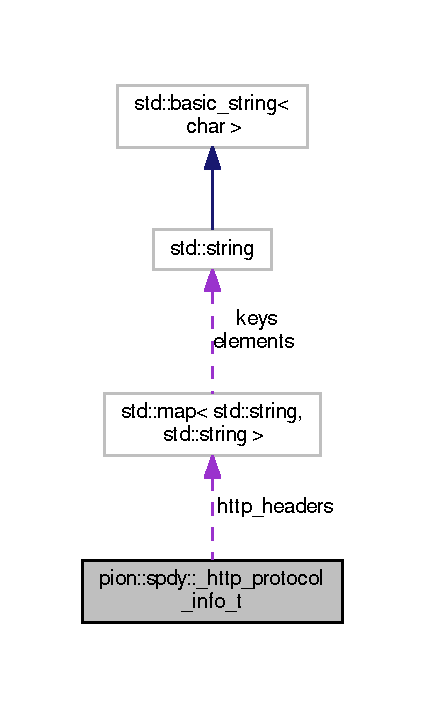
\includegraphics[width=204pt]{structpion_1_1spdy_1_1__http__protocol__info__t__coll__graph}
\end{center}
\end{figure}
\subsection*{Public Member Functions}
\begin{DoxyCompactItemize}
\item 
\hyperlink{structpion_1_1spdy_1_1__http__protocol__info__t_a702945e6cdc007b0788a73dcf014108f}{\-\_\-http\-\_\-protocol\-\_\-info\-\_\-t} ()
\end{DoxyCompactItemize}
\subsection*{Public Attributes}
\begin{DoxyCompactItemize}
\item 
std\-::map$<$ std\-::string, \\*
std\-::string $>$ \hyperlink{structpion_1_1spdy_1_1__http__protocol__info__t_aa5fe851be6df6f20882ecfb4b0a17173}{http\-\_\-headers}
\item 
boost\-::uint32\-\_\-t \hyperlink{structpion_1_1spdy_1_1__http__protocol__info__t_a2b40596ec08c3f01e3b42a3c9f46144f}{http\-\_\-type}
\item 
boost\-::uint32\-\_\-t \hyperlink{structpion_1_1spdy_1_1__http__protocol__info__t_a17e4bd218ca2af1c9441c4d78b33c91a}{stream\-\_\-id}
\item 
boost\-::uint32\-\_\-t \hyperlink{structpion_1_1spdy_1_1__http__protocol__info__t_ac7eaf2e8f75959697589437fa27dff9a}{data\-\_\-offset}
\item 
boost\-::uint32\-\_\-t \hyperlink{structpion_1_1spdy_1_1__http__protocol__info__t_a9f92f9f33b30a85ed7fd1758206d632e}{data\-\_\-size}
\item 
bool \hyperlink{structpion_1_1spdy_1_1__http__protocol__info__t_ab497d1956139ddbe0773fe6515ef72c7}{last\-\_\-chunk}
\end{DoxyCompactItemize}


\subsection{Detailed Description}
This structure contains the H\-T\-T\-P Protocol information. 

\subsection{Constructor \& Destructor Documentation}
\hypertarget{structpion_1_1spdy_1_1__http__protocol__info__t_a702945e6cdc007b0788a73dcf014108f}{\index{pion\-::spdy\-::\-\_\-http\-\_\-protocol\-\_\-info\-\_\-t@{pion\-::spdy\-::\-\_\-http\-\_\-protocol\-\_\-info\-\_\-t}!\-\_\-http\-\_\-protocol\-\_\-info\-\_\-t@{\-\_\-http\-\_\-protocol\-\_\-info\-\_\-t}}
\index{\-\_\-http\-\_\-protocol\-\_\-info\-\_\-t@{\-\_\-http\-\_\-protocol\-\_\-info\-\_\-t}!pion::spdy::_http_protocol_info_t@{pion\-::spdy\-::\-\_\-http\-\_\-protocol\-\_\-info\-\_\-t}}
\subsubsection[{\-\_\-http\-\_\-protocol\-\_\-info\-\_\-t}]{\setlength{\rightskip}{0pt plus 5cm}pion\-::spdy\-::\-\_\-http\-\_\-protocol\-\_\-info\-\_\-t\-::\-\_\-http\-\_\-protocol\-\_\-info\-\_\-t (
\begin{DoxyParamCaption}
{}
\end{DoxyParamCaption}
)\hspace{0.3cm}{\ttfamily [inline]}}}\label{structpion_1_1spdy_1_1__http__protocol__info__t_a702945e6cdc007b0788a73dcf014108f}


\subsection{Member Data Documentation}
\hypertarget{structpion_1_1spdy_1_1__http__protocol__info__t_ac7eaf2e8f75959697589437fa27dff9a}{\index{pion\-::spdy\-::\-\_\-http\-\_\-protocol\-\_\-info\-\_\-t@{pion\-::spdy\-::\-\_\-http\-\_\-protocol\-\_\-info\-\_\-t}!data\-\_\-offset@{data\-\_\-offset}}
\index{data\-\_\-offset@{data\-\_\-offset}!pion::spdy::_http_protocol_info_t@{pion\-::spdy\-::\-\_\-http\-\_\-protocol\-\_\-info\-\_\-t}}
\subsubsection[{data\-\_\-offset}]{\setlength{\rightskip}{0pt plus 5cm}boost\-::uint32\-\_\-t pion\-::spdy\-::\-\_\-http\-\_\-protocol\-\_\-info\-\_\-t\-::data\-\_\-offset}}\label{structpion_1_1spdy_1_1__http__protocol__info__t_ac7eaf2e8f75959697589437fa27dff9a}


Referenced by pion\-::spdy\-::parser\-::populate\-\_\-frame().

\hypertarget{structpion_1_1spdy_1_1__http__protocol__info__t_a9f92f9f33b30a85ed7fd1758206d632e}{\index{pion\-::spdy\-::\-\_\-http\-\_\-protocol\-\_\-info\-\_\-t@{pion\-::spdy\-::\-\_\-http\-\_\-protocol\-\_\-info\-\_\-t}!data\-\_\-size@{data\-\_\-size}}
\index{data\-\_\-size@{data\-\_\-size}!pion::spdy::_http_protocol_info_t@{pion\-::spdy\-::\-\_\-http\-\_\-protocol\-\_\-info\-\_\-t}}
\subsubsection[{data\-\_\-size}]{\setlength{\rightskip}{0pt plus 5cm}boost\-::uint32\-\_\-t pion\-::spdy\-::\-\_\-http\-\_\-protocol\-\_\-info\-\_\-t\-::data\-\_\-size}}\label{structpion_1_1spdy_1_1__http__protocol__info__t_a9f92f9f33b30a85ed7fd1758206d632e}


Referenced by pion\-::spdy\-::parser\-::populate\-\_\-frame().

\hypertarget{structpion_1_1spdy_1_1__http__protocol__info__t_aa5fe851be6df6f20882ecfb4b0a17173}{\index{pion\-::spdy\-::\-\_\-http\-\_\-protocol\-\_\-info\-\_\-t@{pion\-::spdy\-::\-\_\-http\-\_\-protocol\-\_\-info\-\_\-t}!http\-\_\-headers@{http\-\_\-headers}}
\index{http\-\_\-headers@{http\-\_\-headers}!pion::spdy::_http_protocol_info_t@{pion\-::spdy\-::\-\_\-http\-\_\-protocol\-\_\-info\-\_\-t}}
\subsubsection[{http\-\_\-headers}]{\setlength{\rightskip}{0pt plus 5cm}std\-::map$<$std\-::string, std\-::string$>$ pion\-::spdy\-::\-\_\-http\-\_\-protocol\-\_\-info\-\_\-t\-::http\-\_\-headers}}\label{structpion_1_1spdy_1_1__http__protocol__info__t_aa5fe851be6df6f20882ecfb4b0a17173}


Referenced by pion\-::spdy\-::parser\-::parse\-\_\-header\-\_\-payload().

\hypertarget{structpion_1_1spdy_1_1__http__protocol__info__t_a2b40596ec08c3f01e3b42a3c9f46144f}{\index{pion\-::spdy\-::\-\_\-http\-\_\-protocol\-\_\-info\-\_\-t@{pion\-::spdy\-::\-\_\-http\-\_\-protocol\-\_\-info\-\_\-t}!http\-\_\-type@{http\-\_\-type}}
\index{http\-\_\-type@{http\-\_\-type}!pion::spdy::_http_protocol_info_t@{pion\-::spdy\-::\-\_\-http\-\_\-protocol\-\_\-info\-\_\-t}}
\subsubsection[{http\-\_\-type}]{\setlength{\rightskip}{0pt plus 5cm}boost\-::uint32\-\_\-t pion\-::spdy\-::\-\_\-http\-\_\-protocol\-\_\-info\-\_\-t\-::http\-\_\-type}}\label{structpion_1_1spdy_1_1__http__protocol__info__t_a2b40596ec08c3f01e3b42a3c9f46144f}


Referenced by pion\-::spdy\-::parser\-::parse\-\_\-spdy\-\_\-frame().

\hypertarget{structpion_1_1spdy_1_1__http__protocol__info__t_ab497d1956139ddbe0773fe6515ef72c7}{\index{pion\-::spdy\-::\-\_\-http\-\_\-protocol\-\_\-info\-\_\-t@{pion\-::spdy\-::\-\_\-http\-\_\-protocol\-\_\-info\-\_\-t}!last\-\_\-chunk@{last\-\_\-chunk}}
\index{last\-\_\-chunk@{last\-\_\-chunk}!pion::spdy::_http_protocol_info_t@{pion\-::spdy\-::\-\_\-http\-\_\-protocol\-\_\-info\-\_\-t}}
\subsubsection[{last\-\_\-chunk}]{\setlength{\rightskip}{0pt plus 5cm}bool pion\-::spdy\-::\-\_\-http\-\_\-protocol\-\_\-info\-\_\-t\-::last\-\_\-chunk}}\label{structpion_1_1spdy_1_1__http__protocol__info__t_ab497d1956139ddbe0773fe6515ef72c7}


Referenced by pion\-::spdy\-::parser\-::parse\-\_\-spdy\-\_\-data().

\hypertarget{structpion_1_1spdy_1_1__http__protocol__info__t_a17e4bd218ca2af1c9441c4d78b33c91a}{\index{pion\-::spdy\-::\-\_\-http\-\_\-protocol\-\_\-info\-\_\-t@{pion\-::spdy\-::\-\_\-http\-\_\-protocol\-\_\-info\-\_\-t}!stream\-\_\-id@{stream\-\_\-id}}
\index{stream\-\_\-id@{stream\-\_\-id}!pion::spdy::_http_protocol_info_t@{pion\-::spdy\-::\-\_\-http\-\_\-protocol\-\_\-info\-\_\-t}}
\subsubsection[{stream\-\_\-id}]{\setlength{\rightskip}{0pt plus 5cm}boost\-::uint32\-\_\-t pion\-::spdy\-::\-\_\-http\-\_\-protocol\-\_\-info\-\_\-t\-::stream\-\_\-id}}\label{structpion_1_1spdy_1_1__http__protocol__info__t_a17e4bd218ca2af1c9441c4d78b33c91a}


Referenced by pion\-::spdy\-::parser\-::parse\-\_\-header\-\_\-payload(), and pion\-::spdy\-::parser\-::populate\-\_\-frame().



The documentation for this struct was generated from the following file\-:\begin{DoxyCompactItemize}
\item 
include/pion/spdy/\hyperlink{spdy_2types_8hpp}{types.\-hpp}\end{DoxyCompactItemize}

\hypertarget{structpion_1_1spdy_1_1__spdy__header__info}{\section{pion\-:\-:spdy\-:\-:\-\_\-spdy\-\_\-header\-\_\-info Struct Reference}
\label{structpion_1_1spdy_1_1__spdy__header__info}\index{pion\-::spdy\-::\-\_\-spdy\-\_\-header\-\_\-info@{pion\-::spdy\-::\-\_\-spdy\-\_\-header\-\_\-info}}
}


{\ttfamily \#include $<$types.\-hpp$>$}

\subsection*{Public Attributes}
\begin{DoxyCompactItemize}
\item 
boost\-::uint32\-\_\-t \hyperlink{structpion_1_1spdy_1_1__spdy__header__info_a34f64295be06d0aabaf70142f78e3050}{stream\-\_\-id}
\item 
boost\-::uint8\-\_\-t $\ast$ \hyperlink{structpion_1_1spdy_1_1__spdy__header__info_a04e2da993193a952036d13477114bd0e}{header\-\_\-block}
\item 
boost\-::uint8\-\_\-t \hyperlink{structpion_1_1spdy_1_1__spdy__header__info_a0b5e5f60e357c45af5069d8c7e270028}{header\-\_\-block\-\_\-len}
\item 
boost\-::uint16\-\_\-t \hyperlink{structpion_1_1spdy_1_1__spdy__header__info_afa1a89722edd7a2eda6fd7a15abf7e76}{frame\-\_\-type}
\end{DoxyCompactItemize}


\subsection{Detailed Description}
This structure will be tied to each S\-P\-D\-Y header frame. Only applies to frames containing headers\-: S\-Y\-N\-\_\-\-S\-T\-R\-E\-A\-M, S\-Y\-N\-\_\-\-R\-E\-P\-L\-Y, H\-E\-A\-D\-E\-R\-S Note that there may be multiple S\-P\-D\-Y frames in one packet. 

\subsection{Member Data Documentation}
\hypertarget{structpion_1_1spdy_1_1__spdy__header__info_afa1a89722edd7a2eda6fd7a15abf7e76}{\index{pion\-::spdy\-::\-\_\-spdy\-\_\-header\-\_\-info@{pion\-::spdy\-::\-\_\-spdy\-\_\-header\-\_\-info}!frame\-\_\-type@{frame\-\_\-type}}
\index{frame\-\_\-type@{frame\-\_\-type}!pion::spdy::_spdy_header_info@{pion\-::spdy\-::\-\_\-spdy\-\_\-header\-\_\-info}}
\subsubsection[{frame\-\_\-type}]{\setlength{\rightskip}{0pt plus 5cm}boost\-::uint16\-\_\-t pion\-::spdy\-::\-\_\-spdy\-\_\-header\-\_\-info\-::frame\-\_\-type}}\label{structpion_1_1spdy_1_1__spdy__header__info_afa1a89722edd7a2eda6fd7a15abf7e76}
\hypertarget{structpion_1_1spdy_1_1__spdy__header__info_a04e2da993193a952036d13477114bd0e}{\index{pion\-::spdy\-::\-\_\-spdy\-\_\-header\-\_\-info@{pion\-::spdy\-::\-\_\-spdy\-\_\-header\-\_\-info}!header\-\_\-block@{header\-\_\-block}}
\index{header\-\_\-block@{header\-\_\-block}!pion::spdy::_spdy_header_info@{pion\-::spdy\-::\-\_\-spdy\-\_\-header\-\_\-info}}
\subsubsection[{header\-\_\-block}]{\setlength{\rightskip}{0pt plus 5cm}boost\-::uint8\-\_\-t$\ast$ pion\-::spdy\-::\-\_\-spdy\-\_\-header\-\_\-info\-::header\-\_\-block}}\label{structpion_1_1spdy_1_1__spdy__header__info_a04e2da993193a952036d13477114bd0e}
\hypertarget{structpion_1_1spdy_1_1__spdy__header__info_a0b5e5f60e357c45af5069d8c7e270028}{\index{pion\-::spdy\-::\-\_\-spdy\-\_\-header\-\_\-info@{pion\-::spdy\-::\-\_\-spdy\-\_\-header\-\_\-info}!header\-\_\-block\-\_\-len@{header\-\_\-block\-\_\-len}}
\index{header\-\_\-block\-\_\-len@{header\-\_\-block\-\_\-len}!pion::spdy::_spdy_header_info@{pion\-::spdy\-::\-\_\-spdy\-\_\-header\-\_\-info}}
\subsubsection[{header\-\_\-block\-\_\-len}]{\setlength{\rightskip}{0pt plus 5cm}boost\-::uint8\-\_\-t pion\-::spdy\-::\-\_\-spdy\-\_\-header\-\_\-info\-::header\-\_\-block\-\_\-len}}\label{structpion_1_1spdy_1_1__spdy__header__info_a0b5e5f60e357c45af5069d8c7e270028}
\hypertarget{structpion_1_1spdy_1_1__spdy__header__info_a34f64295be06d0aabaf70142f78e3050}{\index{pion\-::spdy\-::\-\_\-spdy\-\_\-header\-\_\-info@{pion\-::spdy\-::\-\_\-spdy\-\_\-header\-\_\-info}!stream\-\_\-id@{stream\-\_\-id}}
\index{stream\-\_\-id@{stream\-\_\-id}!pion::spdy::_spdy_header_info@{pion\-::spdy\-::\-\_\-spdy\-\_\-header\-\_\-info}}
\subsubsection[{stream\-\_\-id}]{\setlength{\rightskip}{0pt plus 5cm}boost\-::uint32\-\_\-t pion\-::spdy\-::\-\_\-spdy\-\_\-header\-\_\-info\-::stream\-\_\-id}}\label{structpion_1_1spdy_1_1__spdy__header__info_a34f64295be06d0aabaf70142f78e3050}


The documentation for this struct was generated from the following file\-:\begin{DoxyCompactItemize}
\item 
include/pion/spdy/\hyperlink{spdy_2types_8hpp}{types.\-hpp}\end{DoxyCompactItemize}

\hypertarget{classpion_1_1admin__rights}{\section{pion\-:\-:admin\-\_\-rights Class Reference}
\label{classpion_1_1admin__rights}\index{pion\-::admin\-\_\-rights@{pion\-::admin\-\_\-rights}}
}


{\ttfamily \#include $<$admin\-\_\-rights.\-hpp$>$}

\subsection*{Public Member Functions}
\begin{DoxyCompactItemize}
\item 
\hyperlink{classpion_1_1admin__rights_abfb9f3aea1e085f4a5a666a98fa36c7c}{admin\-\_\-rights} (bool use\-\_\-log=true)
\item 
virtual \hyperlink{classpion_1_1admin__rights_a3dd9a6d85bdeffe1243a25b78e562716}{$\sim$admin\-\_\-rights} ()
\begin{DoxyCompactList}\small\item\em destructor releases administrative rights \end{DoxyCompactList}\item 
void \hyperlink{classpion_1_1admin__rights_a2979c3b20e89e29113a9593d14a563b8}{release} (void)
\begin{DoxyCompactList}\small\item\em releases administrative rights \end{DoxyCompactList}\end{DoxyCompactItemize}
\subsection*{Static Public Member Functions}
\begin{DoxyCompactItemize}
\item 
static long \hyperlink{classpion_1_1admin__rights_ab8ebba2984ee6610829fbac64c149f06}{run\-\_\-as\-\_\-user} (const std\-::string \&user\-\_\-name)
\begin{DoxyCompactList}\small\item\em calculates the user id based upon the user configuration parameter \end{DoxyCompactList}\item 
static long \hyperlink{classpion_1_1admin__rights_ae2b1e96be191af3cf81851cdf2c69e2a}{run\-\_\-as\-\_\-group} (const std\-::string \&group\-\_\-name)
\begin{DoxyCompactList}\small\item\em calculates the group id based upon the group configuration parameter \end{DoxyCompactList}\end{DoxyCompactItemize}


\subsection{Detailed Description}
\hyperlink{classpion_1_1admin__rights}{admin\-\_\-rights}\-: obtains administrative rights for the process 

\subsection{Constructor \& Destructor Documentation}
\hypertarget{classpion_1_1admin__rights_abfb9f3aea1e085f4a5a666a98fa36c7c}{\index{pion\-::admin\-\_\-rights@{pion\-::admin\-\_\-rights}!admin\-\_\-rights@{admin\-\_\-rights}}
\index{admin\-\_\-rights@{admin\-\_\-rights}!pion::admin_rights@{pion\-::admin\-\_\-rights}}
\subsubsection[{admin\-\_\-rights}]{\setlength{\rightskip}{0pt plus 5cm}pion\-::admin\-\_\-rights\-::admin\-\_\-rights (
\begin{DoxyParamCaption}
\item[{bool}]{use\-\_\-log = {\ttfamily true}}
\end{DoxyParamCaption}
)}}\label{classpion_1_1admin__rights_abfb9f3aea1e085f4a5a666a98fa36c7c}
constructs object, obtaining administrative rights; will block if another thread has already obtained rights


\begin{DoxyParams}{Parameters}
{\em use\-\_\-log} & if false, then no logging will be performed \\
\hline
\end{DoxyParams}


References P\-I\-O\-N\-\_\-\-L\-O\-G\-\_\-\-D\-E\-B\-U\-G, and P\-I\-O\-N\-\_\-\-L\-O\-G\-\_\-\-E\-R\-R\-O\-R.

\hypertarget{classpion_1_1admin__rights_a3dd9a6d85bdeffe1243a25b78e562716}{\index{pion\-::admin\-\_\-rights@{pion\-::admin\-\_\-rights}!$\sim$admin\-\_\-rights@{$\sim$admin\-\_\-rights}}
\index{$\sim$admin\-\_\-rights@{$\sim$admin\-\_\-rights}!pion::admin_rights@{pion\-::admin\-\_\-rights}}
\subsubsection[{$\sim$admin\-\_\-rights}]{\setlength{\rightskip}{0pt plus 5cm}virtual pion\-::admin\-\_\-rights\-::$\sim$admin\-\_\-rights (
\begin{DoxyParamCaption}
{}
\end{DoxyParamCaption}
)\hspace{0.3cm}{\ttfamily [inline]}, {\ttfamily [virtual]}}}\label{classpion_1_1admin__rights_a3dd9a6d85bdeffe1243a25b78e562716}


destructor releases administrative rights 



\subsection{Member Function Documentation}
\hypertarget{classpion_1_1admin__rights_a2979c3b20e89e29113a9593d14a563b8}{\index{pion\-::admin\-\_\-rights@{pion\-::admin\-\_\-rights}!release@{release}}
\index{release@{release}!pion::admin_rights@{pion\-::admin\-\_\-rights}}
\subsubsection[{release}]{\setlength{\rightskip}{0pt plus 5cm}void pion\-::admin\-\_\-rights\-::release (
\begin{DoxyParamCaption}
\item[{void}]{}
\end{DoxyParamCaption}
)}}\label{classpion_1_1admin__rights_a2979c3b20e89e29113a9593d14a563b8}


releases administrative rights 



References P\-I\-O\-N\-\_\-\-L\-O\-G\-\_\-\-D\-E\-B\-U\-G, and P\-I\-O\-N\-\_\-\-L\-O\-G\-\_\-\-E\-R\-R\-O\-R.

\hypertarget{classpion_1_1admin__rights_ae2b1e96be191af3cf81851cdf2c69e2a}{\index{pion\-::admin\-\_\-rights@{pion\-::admin\-\_\-rights}!run\-\_\-as\-\_\-group@{run\-\_\-as\-\_\-group}}
\index{run\-\_\-as\-\_\-group@{run\-\_\-as\-\_\-group}!pion::admin_rights@{pion\-::admin\-\_\-rights}}
\subsubsection[{run\-\_\-as\-\_\-group}]{\setlength{\rightskip}{0pt plus 5cm}long pion\-::admin\-\_\-rights\-::run\-\_\-as\-\_\-group (
\begin{DoxyParamCaption}
\item[{const std\-::string \&}]{group\-\_\-name}
\end{DoxyParamCaption}
)\hspace{0.3cm}{\ttfamily [static]}}}\label{classpion_1_1admin__rights_ae2b1e96be191af3cf81851cdf2c69e2a}


calculates the group id based upon the group configuration parameter 

\hypertarget{classpion_1_1admin__rights_ab8ebba2984ee6610829fbac64c149f06}{\index{pion\-::admin\-\_\-rights@{pion\-::admin\-\_\-rights}!run\-\_\-as\-\_\-user@{run\-\_\-as\-\_\-user}}
\index{run\-\_\-as\-\_\-user@{run\-\_\-as\-\_\-user}!pion::admin_rights@{pion\-::admin\-\_\-rights}}
\subsubsection[{run\-\_\-as\-\_\-user}]{\setlength{\rightskip}{0pt plus 5cm}long pion\-::admin\-\_\-rights\-::run\-\_\-as\-\_\-user (
\begin{DoxyParamCaption}
\item[{const std\-::string \&}]{user\-\_\-name}
\end{DoxyParamCaption}
)\hspace{0.3cm}{\ttfamily [static]}}}\label{classpion_1_1admin__rights_ab8ebba2984ee6610829fbac64c149f06}


calculates the user id based upon the user configuration parameter 



The documentation for this class was generated from the following files\-:\begin{DoxyCompactItemize}
\item 
include/pion/\hyperlink{admin__rights_8hpp}{admin\-\_\-rights.\-hpp}\item 
src/\hyperlink{admin__rights_8cpp}{admin\-\_\-rights.\-cpp}\end{DoxyCompactItemize}

\hypertarget{structpion_1_1algorithm}{\section{pion\-:\-:algorithm Struct Reference}
\label{structpion_1_1algorithm}\index{pion\-::algorithm@{pion\-::algorithm}}
}


{\ttfamily \#include $<$algorithm.\-hpp$>$}

\subsection*{Static Public Member Functions}
\begin{DoxyCompactItemize}
\item 
static bool \hyperlink{structpion_1_1algorithm_ad1700ce7cf8e29bb7600d5729fd4cdad}{base64\-\_\-decode} (std\-::string const \&input, std\-::string \&output)
\item 
static bool \hyperlink{structpion_1_1algorithm_ae5f52e52ac349ecf20410f2ad3e257dd}{base64\-\_\-encode} (std\-::string const \&input, std\-::string \&output)
\item 
static std\-::string \hyperlink{structpion_1_1algorithm_a440bd54b07a24c80bc939fdb03583721}{url\-\_\-decode} (const std\-::string \&str)
\begin{DoxyCompactList}\small\item\em escapes U\-R\-L-\/encoded strings (a\%20value+with\%20spaces) \end{DoxyCompactList}\item 
static std\-::string \hyperlink{structpion_1_1algorithm_aa4eaedaecac95a638cedf5c4884de1b8}{url\-\_\-encode} (const std\-::string \&str)
\begin{DoxyCompactList}\small\item\em encodes strings so that they are safe for U\-R\-Ls (with\%20spaces) \end{DoxyCompactList}\item 
static std\-::string \hyperlink{structpion_1_1algorithm_a2177ca0d0f01e6ef6d4d3bceb73d82bb}{xml\-\_\-encode} (const std\-::string \&str)
\begin{DoxyCompactList}\small\item\em T\-O\-D\-O\-: escapes X\-M\-L/\-H\-T\-M\-L-\/encoded strings (1 $<$ 2) \end{DoxyCompactList}\item 
static void \hyperlink{structpion_1_1algorithm_ab3cce74846661c3585ec5f540a99ff07}{float\-\_\-from\-\_\-bytes} (long double \&value, const unsigned char $\ast$ptr, size\-\_\-t num\-\_\-exp\-\_\-bits, size\-\_\-t num\-\_\-fraction\-\_\-bits)
\item 
static void \hyperlink{structpion_1_1algorithm_a61872c7ccf75793a16d8ce7961f28842}{float\-\_\-to\-\_\-bytes} (long double value, unsigned char $\ast$ptr, size\-\_\-t num\-\_\-exp\-\_\-bits, size\-\_\-t num\-\_\-fraction\-\_\-bits)
\item 
static boost\-::uint8\-\_\-t \hyperlink{structpion_1_1algorithm_a79898e00c20439125c68d90248afb2e0}{to\-\_\-uint8} (unsigned char byte)
\begin{DoxyCompactList}\small\item\em convert sequence of one byte to 8-\/bit unsigned integer \end{DoxyCompactList}\item 
static boost\-::int8\-\_\-t \hyperlink{structpion_1_1algorithm_afb09388ae577897cd3fac5572c9e4eef}{to\-\_\-int8} (unsigned char byte)
\begin{DoxyCompactList}\small\item\em convert sequence of one byte to 8-\/bit signed integer \end{DoxyCompactList}\item 
static boost\-::uint8\-\_\-t \hyperlink{structpion_1_1algorithm_a6088634700c44316b7d6d55e687d65aa}{to\-\_\-uint8} (char byte)
\begin{DoxyCompactList}\small\item\em convert sequence of one byte to 8-\/bit unsigned integer \end{DoxyCompactList}\item 
static boost\-::int8\-\_\-t \hyperlink{structpion_1_1algorithm_a8a891be43c16371c9cf9447224f1705c}{to\-\_\-int8} (char byte)
\begin{DoxyCompactList}\small\item\em convert sequence of one byte to 8-\/bit signed integer \end{DoxyCompactList}\item 
static boost\-::uint16\-\_\-t \hyperlink{structpion_1_1algorithm_aa755b157b2cda061aec92c49b7ee9dac}{to\-\_\-uint16} (unsigned char high, unsigned char low)
\begin{DoxyCompactList}\small\item\em convert sequence of two bytes to 16-\/bit unsigned integer \end{DoxyCompactList}\item 
static boost\-::int16\-\_\-t \hyperlink{structpion_1_1algorithm_a32a9690172523ef7c558f92b319429c9}{to\-\_\-int16} (unsigned char high, unsigned char low)
\begin{DoxyCompactList}\small\item\em convert sequence of two bytes to 16-\/bit signed integer \end{DoxyCompactList}\item 
static boost\-::uint32\-\_\-t \hyperlink{structpion_1_1algorithm_ad1fd95bf2a6c3c2a775492c1acd0b5c1}{to\-\_\-uint24} (unsigned char high, unsigned char mid, unsigned char low)
\begin{DoxyCompactList}\small\item\em convert sequence of three bytes to 24-\/bit unsigned integer \end{DoxyCompactList}\item 
static boost\-::int32\-\_\-t \hyperlink{structpion_1_1algorithm_a607abc832ec9f6983cb42b76cc8914e6}{to\-\_\-int24} (unsigned char high, unsigned char mid, unsigned char low)
\begin{DoxyCompactList}\small\item\em convert sequence of three bytes to 24-\/bit signed integer \end{DoxyCompactList}\item 
static boost\-::uint32\-\_\-t \hyperlink{structpion_1_1algorithm_af2092366e2a82fbfc456bceb15a0f599}{to\-\_\-uint32} (unsigned char high, unsigned char mid1, unsigned char mid2, unsigned char low)
\begin{DoxyCompactList}\small\item\em convert sequence of four bytes to 32-\/bit unsigned integer \end{DoxyCompactList}\item 
static boost\-::int32\-\_\-t \hyperlink{structpion_1_1algorithm_ac8dd9cfadaa3fb758b4ea3f9bd524595}{to\-\_\-int32} (unsigned char high, unsigned char mid1, unsigned char mid2, unsigned char low)
\begin{DoxyCompactList}\small\item\em convert sequence of four bytes to 32-\/bit signed integer \end{DoxyCompactList}\item 
static boost\-::uint64\-\_\-t \hyperlink{structpion_1_1algorithm_ab4622cfb454d0ca206ffe42077a15c52}{to\-\_\-uint64} (unsigned char high, unsigned char mid1, unsigned char mid2, unsigned char mid3, unsigned char mid4, unsigned char mid5, unsigned char mid6, unsigned char low)
\begin{DoxyCompactList}\small\item\em convert sequence of eight bytes to 64-\/bit unsigned integer \end{DoxyCompactList}\item 
static boost\-::int64\-\_\-t \hyperlink{structpion_1_1algorithm_aa08271822b58fa0ca87fb4f0740b1d3a}{to\-\_\-int64} (unsigned char high, unsigned char mid1, unsigned char mid2, unsigned char mid3, unsigned char mid4, unsigned char mid5, unsigned char mid6, unsigned char low)
\begin{DoxyCompactList}\small\item\em convert sequence of eight bytes to 64-\/bit signed integer \end{DoxyCompactList}\item 
{\footnotesize template$<$typename T1 , typename T2 $>$ }\\static boost\-::uint16\-\_\-t \hyperlink{structpion_1_1algorithm_a260aedfd03824ec43e7a11a9bb410b69}{to\-\_\-uint16} (T1 high, T2 low)
\begin{DoxyCompactList}\small\item\em convert sequence of two bytes to 16-\/bit unsigned integer \end{DoxyCompactList}\item 
{\footnotesize template$<$typename T1 , typename T2 $>$ }\\static boost\-::int16\-\_\-t \hyperlink{structpion_1_1algorithm_ae474bcdaf7b1a54182e1724c8ebe3410}{to\-\_\-int16} (T1 high, T2 low)
\begin{DoxyCompactList}\small\item\em convert sequence of two bytes to 16-\/bit signed integer \end{DoxyCompactList}\item 
{\footnotesize template$<$typename T1 , typename T2 , typename T3 $>$ }\\static boost\-::uint32\-\_\-t \hyperlink{structpion_1_1algorithm_a1080e1965b34717702987a559665a8e9}{to\-\_\-uint24} (T1 high, T2 mid, T3 low)
\begin{DoxyCompactList}\small\item\em convert sequence of three bytes to 24-\/bit unsigned integer \end{DoxyCompactList}\item 
{\footnotesize template$<$typename T1 , typename T2 , typename T3 $>$ }\\static boost\-::int32\-\_\-t \hyperlink{structpion_1_1algorithm_aed87f4efd146f0d6afdedc8618dfac9c}{to\-\_\-int24} (T1 high, T2 mid, T3 low)
\begin{DoxyCompactList}\small\item\em convert sequence of three bytes to 24-\/bit signed integer \end{DoxyCompactList}\item 
{\footnotesize template$<$typename T1 , typename T2 , typename T3 , typename T4 $>$ }\\static boost\-::uint32\-\_\-t \hyperlink{structpion_1_1algorithm_a14437094ac2afa2b8b2f94a92baf7253}{to\-\_\-uint32} (T1 high, T2 mid1, T3 mid2, T4 low)
\begin{DoxyCompactList}\small\item\em convert sequence of four bytes to 32-\/bit unsigned integer \end{DoxyCompactList}\item 
{\footnotesize template$<$typename T1 , typename T2 , typename T3 , typename T4 $>$ }\\static boost\-::int32\-\_\-t \hyperlink{structpion_1_1algorithm_abad3afe7cdb40f779cac637f3e28702c}{to\-\_\-int32} (T1 high, T2 mid1, T3 mid2, T4 low)
\begin{DoxyCompactList}\small\item\em convert sequence of four bytes to 32-\/bit signed integer \end{DoxyCompactList}\item 
{\footnotesize template$<$typename T1 , typename T2 , typename T3 , typename T4 , typename T5 , typename T6 , typename T7 , typename T8 $>$ }\\static boost\-::uint64\-\_\-t \hyperlink{structpion_1_1algorithm_adae7fcd4321444d86e98acf5796ecadd}{to\-\_\-uint64} (T1 high, T2 mid1, T3 mid2, T4 mid3, T5 mid4, T6 mid5, T7 mid6, T8 low)
\begin{DoxyCompactList}\small\item\em convert sequence of eight bytes to 64-\/bit unsigned integer \end{DoxyCompactList}\item 
{\footnotesize template$<$typename T1 , typename T2 , typename T3 , typename T4 , typename T5 , typename T6 , typename T7 , typename T8 $>$ }\\static boost\-::int64\-\_\-t \hyperlink{structpion_1_1algorithm_a559bde18e9670cefd4c4937394f2c82c}{to\-\_\-int64} (T1 high, T2 mid1, T3 mid2, T4 mid3, T5 mid4, T6 mid5, T7 mid6, T8 low)
\begin{DoxyCompactList}\small\item\em convert sequence of eight bytes to 64-\/bit signed integer \end{DoxyCompactList}\item 
{\footnotesize template$<$typename Byte $>$ }\\static boost\-::uint8\-\_\-t \hyperlink{structpion_1_1algorithm_a60bfca7cfacf90a664a4977cd70ccf68}{to\-\_\-uint8} (const Byte $\ast$buf)
\begin{DoxyCompactList}\small\item\em convert byte pointer into an 8-\/bit unsigned integer \end{DoxyCompactList}\item 
{\footnotesize template$<$typename Byte $>$ }\\static boost\-::int8\-\_\-t \hyperlink{structpion_1_1algorithm_a884a55189c818f89a88ac6791e79de96}{to\-\_\-int8} (const Byte $\ast$buf)
\begin{DoxyCompactList}\small\item\em convert byte pointer into an 8-\/bit signed integer \end{DoxyCompactList}\item 
{\footnotesize template$<$typename Byte $>$ }\\static boost\-::uint16\-\_\-t \hyperlink{structpion_1_1algorithm_a009df038f511d87e4ccb89163305a42b}{to\-\_\-uint16} (const Byte $\ast$buf)
\begin{DoxyCompactList}\small\item\em convert sequence of two bytes to 16-\/bit unsigned integer \end{DoxyCompactList}\item 
{\footnotesize template$<$typename Byte $>$ }\\static boost\-::int16\-\_\-t \hyperlink{structpion_1_1algorithm_a8a5dc0884a7dd1deb53762947dce167c}{to\-\_\-int16} (const Byte $\ast$buf)
\begin{DoxyCompactList}\small\item\em convert sequence of two bytes to 16-\/bit signed integer \end{DoxyCompactList}\item 
{\footnotesize template$<$typename Byte $>$ }\\static boost\-::uint32\-\_\-t \hyperlink{structpion_1_1algorithm_ae54ebabcc5db708e1528c6afd4bb23fc}{to\-\_\-uint24} (const Byte $\ast$buf)
\begin{DoxyCompactList}\small\item\em convert sequence of three bytes to 24-\/bit unsigned integer \end{DoxyCompactList}\item 
{\footnotesize template$<$typename Byte $>$ }\\static boost\-::int32\-\_\-t \hyperlink{structpion_1_1algorithm_aa7faf5f422723c835e432e6c0bd43a71}{to\-\_\-int24} (const Byte $\ast$buf)
\begin{DoxyCompactList}\small\item\em convert sequence of three bytes to 24-\/bit signed integer \end{DoxyCompactList}\item 
{\footnotesize template$<$typename Byte $>$ }\\static boost\-::uint32\-\_\-t \hyperlink{structpion_1_1algorithm_ad8e9e4a781ab4c3903f53b771239bad3}{to\-\_\-uint32} (const Byte $\ast$buf)
\begin{DoxyCompactList}\small\item\em convert sequence of four bytes to 32-\/bit unsigned integer \end{DoxyCompactList}\item 
{\footnotesize template$<$typename Byte $>$ }\\static boost\-::int32\-\_\-t \hyperlink{structpion_1_1algorithm_a1f6f08fd741bd53e2d7ab23d13d557ec}{to\-\_\-int32} (const Byte $\ast$buf)
\begin{DoxyCompactList}\small\item\em convert sequence of four bytes to 32-\/bit signed integer \end{DoxyCompactList}\item 
{\footnotesize template$<$typename Byte $>$ }\\static boost\-::uint64\-\_\-t \hyperlink{structpion_1_1algorithm_a6043289280973a9c81c3f227f7be3558}{to\-\_\-uint64} (const Byte $\ast$buf)
\begin{DoxyCompactList}\small\item\em convert sequence of eight bytes to 64-\/bit unsigned integer \end{DoxyCompactList}\item 
{\footnotesize template$<$typename Byte $>$ }\\static boost\-::int64\-\_\-t \hyperlink{structpion_1_1algorithm_a320eb1084a7f4c6721aa4c5c1f212c76}{to\-\_\-int64} (const Byte $\ast$buf)
\begin{DoxyCompactList}\small\item\em convert sequence of eight bytes to 64-\/bit signed integer \end{DoxyCompactList}\item 
{\footnotesize template$<$typename Byte $>$ }\\static void \hyperlink{structpion_1_1algorithm_a8ef52bc60dfefc940b6fdf5a1dcb5ad7}{from\-\_\-uint8} (Byte $\ast$buf, const boost\-::uint8\-\_\-t n)
\begin{DoxyCompactList}\small\item\em convert 8-\/bit unsigned integer into sequence of one byte \end{DoxyCompactList}\item 
{\footnotesize template$<$typename Byte $>$ }\\static void \hyperlink{structpion_1_1algorithm_aaf784c8b8c422a15929fb1486d3a7282}{from\-\_\-int8} (Byte $\ast$buf, const boost\-::int8\-\_\-t n)
\begin{DoxyCompactList}\small\item\em convert 8-\/bit signed integer into sequence of one byte \end{DoxyCompactList}\item 
{\footnotesize template$<$typename Byte $>$ }\\static void \hyperlink{structpion_1_1algorithm_a9c5dbfc05e297e824b47e03c6cf4ce26}{from\-\_\-uint16} (Byte $\ast$buf, const boost\-::uint16\-\_\-t n)
\begin{DoxyCompactList}\small\item\em convert 16-\/bit unsigned integer into sequence of two bytes \end{DoxyCompactList}\item 
{\footnotesize template$<$typename Byte $>$ }\\static void \hyperlink{structpion_1_1algorithm_a7668dc2bd3cc56d59353e8664ca128d5}{from\-\_\-int16} (Byte $\ast$buf, const boost\-::int16\-\_\-t n)
\begin{DoxyCompactList}\small\item\em convert 16-\/bit signed integer into sequence of two bytes \end{DoxyCompactList}\item 
{\footnotesize template$<$typename Byte $>$ }\\static void \hyperlink{structpion_1_1algorithm_a72de6ae9d5cee3b2fed7014a0bbe612c}{from\-\_\-uint24} (Byte $\ast$buf, const boost\-::uint32\-\_\-t n)
\begin{DoxyCompactList}\small\item\em convert 24-\/bit unsigned integer into sequence of three bytes \end{DoxyCompactList}\item 
{\footnotesize template$<$typename Byte $>$ }\\static void \hyperlink{structpion_1_1algorithm_ada38cebfc1f9988ee34695663e260abb}{from\-\_\-int24} (Byte $\ast$buf, const boost\-::int32\-\_\-t n)
\begin{DoxyCompactList}\small\item\em convert 24-\/bit signed integer into sequence of three bytes \end{DoxyCompactList}\item 
{\footnotesize template$<$typename Byte $>$ }\\static void \hyperlink{structpion_1_1algorithm_a5c78cafafadb680180ff97f1eaf58fce}{from\-\_\-uint32} (Byte $\ast$buf, const boost\-::uint32\-\_\-t n)
\begin{DoxyCompactList}\small\item\em convert 32-\/bit unsigned integer into sequence of four bytes \end{DoxyCompactList}\item 
{\footnotesize template$<$typename Byte $>$ }\\static void \hyperlink{structpion_1_1algorithm_acea1222844d4cb2fa93cd2510999e376}{from\-\_\-int32} (Byte $\ast$buf, const boost\-::int32\-\_\-t n)
\begin{DoxyCompactList}\small\item\em convert 32-\/bit signed integer into sequence of four bytes \end{DoxyCompactList}\item 
{\footnotesize template$<$typename Byte $>$ }\\static void \hyperlink{structpion_1_1algorithm_a5b030d4284869249e23311d75eaedd57}{from\-\_\-uint64} (Byte $\ast$buf, const boost\-::uint64\-\_\-t n)
\begin{DoxyCompactList}\small\item\em convert 64-\/bit unsigned integer into sequence of eight bytes \end{DoxyCompactList}\item 
{\footnotesize template$<$typename Byte $>$ }\\static void \hyperlink{structpion_1_1algorithm_ad89ffdbdeab62a40643b566a166ec726}{from\-\_\-int64} (Byte $\ast$buf, const boost\-::int64\-\_\-t n)
\begin{DoxyCompactList}\small\item\em convert 64-\/bit signed integer into sequence of eight bytes \end{DoxyCompactList}\item 
{\footnotesize template$<$typename Byte $>$ }\\static float \hyperlink{structpion_1_1algorithm_a31acba5139987280e2d51aeb48f21f28}{to\-\_\-float} (const Byte $\ast$ptr)
\item 
{\footnotesize template$<$typename Byte $>$ }\\static double \hyperlink{structpion_1_1algorithm_a00b83de67d45aceec623296314885f81}{to\-\_\-double} (const Byte $\ast$ptr)
\item 
{\footnotesize template$<$typename Byte $>$ }\\static long double \hyperlink{structpion_1_1algorithm_aad9a66169d2c5a3b009ae25255775cf0}{to\-\_\-long\-\_\-double} (const Byte $\ast$ptr)
\item 
{\footnotesize template$<$typename Byte $>$ }\\static void \hyperlink{structpion_1_1algorithm_a281972f7e3f6a234080e1c792d920723}{from\-\_\-float} (Byte $\ast$ptr, const float n)
\item 
{\footnotesize template$<$typename Byte $>$ }\\static void \hyperlink{structpion_1_1algorithm_a241c29e87904952a01f40624d5494aef}{from\-\_\-double} (Byte $\ast$ptr, const double n)
\item 
{\footnotesize template$<$typename Byte $>$ }\\static void \hyperlink{structpion_1_1algorithm_a387c15c00a1d229059e9da8ff9e0aa84}{from\-\_\-long\-\_\-double} (Byte $\ast$ptr, const long double n)
\end{DoxyCompactItemize}
\subsection*{Static Public Attributes}
\begin{DoxyCompactItemize}
\item 
static const char $\ast$const \hyperlink{structpion_1_1algorithm_ad068c4b57bfaefc287dcda5681095603}{U\-T\-F8\-\_\-\-R\-E\-P\-L\-A\-C\-E\-M\-E\-N\-T\-\_\-\-C\-H\-A\-R} = \char`\"{}\textbackslash{}x\-E\-F\textbackslash{}x\-B\-F\textbackslash{}x\-B\-D\char`\"{}
\begin{DoxyCompactList}\small\item\em 3-\/byte character sequence representing the U\-T\-F-\/8 replacement character \end{DoxyCompactList}\end{DoxyCompactItemize}


\subsection{Member Function Documentation}
\hypertarget{structpion_1_1algorithm_ad1700ce7cf8e29bb7600d5729fd4cdad}{\index{pion\-::algorithm@{pion\-::algorithm}!base64\-\_\-decode@{base64\-\_\-decode}}
\index{base64\-\_\-decode@{base64\-\_\-decode}!pion::algorithm@{pion\-::algorithm}}
\subsubsection[{base64\-\_\-decode}]{\setlength{\rightskip}{0pt plus 5cm}bool pion\-::algorithm\-::base64\-\_\-decode (
\begin{DoxyParamCaption}
\item[{std\-::string const \&}]{input, }
\item[{std\-::string \&}]{output}
\end{DoxyParamCaption}
)\hspace{0.3cm}{\ttfamily [static]}}}\label{structpion_1_1algorithm_ad1700ce7cf8e29bb7600d5729fd4cdad}
base64 decoding


\begin{DoxyParams}{Parameters}
{\em input} & -\/ base64 encoded string \\
\hline
{\em output} & -\/ decoded string ( may include non-\/text chars) \\
\hline
\end{DoxyParams}
\begin{DoxyReturn}{Returns}
true if successful, false if input string contains non-\/base64 symbols 
\end{DoxyReturn}


Referenced by pion\-::http\-::basic\-\_\-auth\-::parse\-\_\-credentials().

\hypertarget{structpion_1_1algorithm_ae5f52e52ac349ecf20410f2ad3e257dd}{\index{pion\-::algorithm@{pion\-::algorithm}!base64\-\_\-encode@{base64\-\_\-encode}}
\index{base64\-\_\-encode@{base64\-\_\-encode}!pion::algorithm@{pion\-::algorithm}}
\subsubsection[{base64\-\_\-encode}]{\setlength{\rightskip}{0pt plus 5cm}bool pion\-::algorithm\-::base64\-\_\-encode (
\begin{DoxyParamCaption}
\item[{std\-::string const \&}]{input, }
\item[{std\-::string \&}]{output}
\end{DoxyParamCaption}
)\hspace{0.3cm}{\ttfamily [static]}}}\label{structpion_1_1algorithm_ae5f52e52ac349ecf20410f2ad3e257dd}
base64 encoding


\begin{DoxyParams}{Parameters}
{\em input} & -\/ arbitrary string ( may include non-\/text chars) \\
\hline
{\em output} & -\/ base64 encoded string \\
\hline
\end{DoxyParams}
\begin{DoxyReturn}{Returns}
true if successful, 
\end{DoxyReturn}


Referenced by pion\-::http\-::cookie\-\_\-auth\-::process\-\_\-login().

\hypertarget{structpion_1_1algorithm_ab3cce74846661c3585ec5f540a99ff07}{\index{pion\-::algorithm@{pion\-::algorithm}!float\-\_\-from\-\_\-bytes@{float\-\_\-from\-\_\-bytes}}
\index{float\-\_\-from\-\_\-bytes@{float\-\_\-from\-\_\-bytes}!pion::algorithm@{pion\-::algorithm}}
\subsubsection[{float\-\_\-from\-\_\-bytes}]{\setlength{\rightskip}{0pt plus 5cm}void pion\-::algorithm\-::float\-\_\-from\-\_\-bytes (
\begin{DoxyParamCaption}
\item[{long double \&}]{value, }
\item[{const unsigned char $\ast$}]{ptr, }
\item[{size\-\_\-t}]{num\-\_\-exp\-\_\-bits, }
\item[{size\-\_\-t}]{num\-\_\-fraction\-\_\-bits}
\end{DoxyParamCaption}
)\hspace{0.3cm}{\ttfamily [static]}}}\label{structpion_1_1algorithm_ab3cce74846661c3585ec5f540a99ff07}
convert sequence of bytes in I\-E\-E\-E 754 format into a native floating point data type reference\-: \href{http://en.wikipedia.org/wiki/Single_precision_floating-point_format}{\tt http\-://en.\-wikipedia.\-org/wiki/\-Single\-\_\-precision\-\_\-floating-\/point\-\_\-format} 

References S\-H\-I\-F\-T\-\_\-\-B\-I\-T\-M\-A\-S\-K.

\hypertarget{structpion_1_1algorithm_a61872c7ccf75793a16d8ce7961f28842}{\index{pion\-::algorithm@{pion\-::algorithm}!float\-\_\-to\-\_\-bytes@{float\-\_\-to\-\_\-bytes}}
\index{float\-\_\-to\-\_\-bytes@{float\-\_\-to\-\_\-bytes}!pion::algorithm@{pion\-::algorithm}}
\subsubsection[{float\-\_\-to\-\_\-bytes}]{\setlength{\rightskip}{0pt plus 5cm}void pion\-::algorithm\-::float\-\_\-to\-\_\-bytes (
\begin{DoxyParamCaption}
\item[{long double}]{value, }
\item[{unsigned char $\ast$}]{ptr, }
\item[{size\-\_\-t}]{num\-\_\-exp\-\_\-bits, }
\item[{size\-\_\-t}]{num\-\_\-fraction\-\_\-bits}
\end{DoxyParamCaption}
)\hspace{0.3cm}{\ttfamily [static]}}}\label{structpion_1_1algorithm_a61872c7ccf75793a16d8ce7961f28842}
convert native floating point type into a sequence of bytes in I\-E\-E\-E 754 format reference\-: \href{http://en.wikipedia.org/wiki/Single_precision_floating-point_format}{\tt http\-://en.\-wikipedia.\-org/wiki/\-Single\-\_\-precision\-\_\-floating-\/point\-\_\-format} 

References S\-H\-I\-F\-T\-\_\-\-B\-I\-T\-M\-A\-S\-K.

\hypertarget{structpion_1_1algorithm_a241c29e87904952a01f40624d5494aef}{\index{pion\-::algorithm@{pion\-::algorithm}!from\-\_\-double@{from\-\_\-double}}
\index{from\-\_\-double@{from\-\_\-double}!pion::algorithm@{pion\-::algorithm}}
\subsubsection[{from\-\_\-double}]{\setlength{\rightskip}{0pt plus 5cm}template$<$typename Byte $>$ static void pion\-::algorithm\-::from\-\_\-double (
\begin{DoxyParamCaption}
\item[{Byte $\ast$}]{ptr, }
\item[{const double}]{n}
\end{DoxyParamCaption}
)\hspace{0.3cm}{\ttfamily [inline]}, {\ttfamily [static]}}}\label{structpion_1_1algorithm_a241c29e87904952a01f40624d5494aef}
convert double into sequence of eight bytes in \char`\"{}double precision\char`\"{} binary64 format \href{http://en.wikipedia.org/wiki/Double_precision_floating-point_format}{\tt http\-://en.\-wikipedia.\-org/wiki/\-Double\-\_\-precision\-\_\-floating-\/point\-\_\-format} \hypertarget{structpion_1_1algorithm_a281972f7e3f6a234080e1c792d920723}{\index{pion\-::algorithm@{pion\-::algorithm}!from\-\_\-float@{from\-\_\-float}}
\index{from\-\_\-float@{from\-\_\-float}!pion::algorithm@{pion\-::algorithm}}
\subsubsection[{from\-\_\-float}]{\setlength{\rightskip}{0pt plus 5cm}template$<$typename Byte $>$ static void pion\-::algorithm\-::from\-\_\-float (
\begin{DoxyParamCaption}
\item[{Byte $\ast$}]{ptr, }
\item[{const float}]{n}
\end{DoxyParamCaption}
)\hspace{0.3cm}{\ttfamily [inline]}, {\ttfamily [static]}}}\label{structpion_1_1algorithm_a281972f7e3f6a234080e1c792d920723}
convert float into sequence of four bytes in \char`\"{}single precision\char`\"{} binary32 format \href{http://en.wikipedia.org/wiki/Single_precision_floating-point_format}{\tt http\-://en.\-wikipedia.\-org/wiki/\-Single\-\_\-precision\-\_\-floating-\/point\-\_\-format} \hypertarget{structpion_1_1algorithm_a7668dc2bd3cc56d59353e8664ca128d5}{\index{pion\-::algorithm@{pion\-::algorithm}!from\-\_\-int16@{from\-\_\-int16}}
\index{from\-\_\-int16@{from\-\_\-int16}!pion::algorithm@{pion\-::algorithm}}
\subsubsection[{from\-\_\-int16}]{\setlength{\rightskip}{0pt plus 5cm}template$<$typename Byte $>$ static void pion\-::algorithm\-::from\-\_\-int16 (
\begin{DoxyParamCaption}
\item[{Byte $\ast$}]{buf, }
\item[{const boost\-::int16\-\_\-t}]{n}
\end{DoxyParamCaption}
)\hspace{0.3cm}{\ttfamily [inline]}, {\ttfamily [static]}}}\label{structpion_1_1algorithm_a7668dc2bd3cc56d59353e8664ca128d5}


convert 16-\/bit signed integer into sequence of two bytes 

\hypertarget{structpion_1_1algorithm_ada38cebfc1f9988ee34695663e260abb}{\index{pion\-::algorithm@{pion\-::algorithm}!from\-\_\-int24@{from\-\_\-int24}}
\index{from\-\_\-int24@{from\-\_\-int24}!pion::algorithm@{pion\-::algorithm}}
\subsubsection[{from\-\_\-int24}]{\setlength{\rightskip}{0pt plus 5cm}template$<$typename Byte $>$ static void pion\-::algorithm\-::from\-\_\-int24 (
\begin{DoxyParamCaption}
\item[{Byte $\ast$}]{buf, }
\item[{const boost\-::int32\-\_\-t}]{n}
\end{DoxyParamCaption}
)\hspace{0.3cm}{\ttfamily [inline]}, {\ttfamily [static]}}}\label{structpion_1_1algorithm_ada38cebfc1f9988ee34695663e260abb}


convert 24-\/bit signed integer into sequence of three bytes 

\hypertarget{structpion_1_1algorithm_acea1222844d4cb2fa93cd2510999e376}{\index{pion\-::algorithm@{pion\-::algorithm}!from\-\_\-int32@{from\-\_\-int32}}
\index{from\-\_\-int32@{from\-\_\-int32}!pion::algorithm@{pion\-::algorithm}}
\subsubsection[{from\-\_\-int32}]{\setlength{\rightskip}{0pt plus 5cm}template$<$typename Byte $>$ static void pion\-::algorithm\-::from\-\_\-int32 (
\begin{DoxyParamCaption}
\item[{Byte $\ast$}]{buf, }
\item[{const boost\-::int32\-\_\-t}]{n}
\end{DoxyParamCaption}
)\hspace{0.3cm}{\ttfamily [inline]}, {\ttfamily [static]}}}\label{structpion_1_1algorithm_acea1222844d4cb2fa93cd2510999e376}


convert 32-\/bit signed integer into sequence of four bytes 

\hypertarget{structpion_1_1algorithm_ad89ffdbdeab62a40643b566a166ec726}{\index{pion\-::algorithm@{pion\-::algorithm}!from\-\_\-int64@{from\-\_\-int64}}
\index{from\-\_\-int64@{from\-\_\-int64}!pion::algorithm@{pion\-::algorithm}}
\subsubsection[{from\-\_\-int64}]{\setlength{\rightskip}{0pt plus 5cm}template$<$typename Byte $>$ static void pion\-::algorithm\-::from\-\_\-int64 (
\begin{DoxyParamCaption}
\item[{Byte $\ast$}]{buf, }
\item[{const boost\-::int64\-\_\-t}]{n}
\end{DoxyParamCaption}
)\hspace{0.3cm}{\ttfamily [inline]}, {\ttfamily [static]}}}\label{structpion_1_1algorithm_ad89ffdbdeab62a40643b566a166ec726}


convert 64-\/bit signed integer into sequence of eight bytes 

\hypertarget{structpion_1_1algorithm_aaf784c8b8c422a15929fb1486d3a7282}{\index{pion\-::algorithm@{pion\-::algorithm}!from\-\_\-int8@{from\-\_\-int8}}
\index{from\-\_\-int8@{from\-\_\-int8}!pion::algorithm@{pion\-::algorithm}}
\subsubsection[{from\-\_\-int8}]{\setlength{\rightskip}{0pt plus 5cm}template$<$typename Byte $>$ static void pion\-::algorithm\-::from\-\_\-int8 (
\begin{DoxyParamCaption}
\item[{Byte $\ast$}]{buf, }
\item[{const boost\-::int8\-\_\-t}]{n}
\end{DoxyParamCaption}
)\hspace{0.3cm}{\ttfamily [inline]}, {\ttfamily [static]}}}\label{structpion_1_1algorithm_aaf784c8b8c422a15929fb1486d3a7282}


convert 8-\/bit signed integer into sequence of one byte 

\hypertarget{structpion_1_1algorithm_a387c15c00a1d229059e9da8ff9e0aa84}{\index{pion\-::algorithm@{pion\-::algorithm}!from\-\_\-long\-\_\-double@{from\-\_\-long\-\_\-double}}
\index{from\-\_\-long\-\_\-double@{from\-\_\-long\-\_\-double}!pion::algorithm@{pion\-::algorithm}}
\subsubsection[{from\-\_\-long\-\_\-double}]{\setlength{\rightskip}{0pt plus 5cm}template$<$typename Byte $>$ static void pion\-::algorithm\-::from\-\_\-long\-\_\-double (
\begin{DoxyParamCaption}
\item[{Byte $\ast$}]{ptr, }
\item[{const long double}]{n}
\end{DoxyParamCaption}
)\hspace{0.3cm}{\ttfamily [inline]}, {\ttfamily [static]}}}\label{structpion_1_1algorithm_a387c15c00a1d229059e9da8ff9e0aa84}
convert long double into sequence of sixteen bytes in 128-\/bit \char`\"{}quadruple precision\char`\"{} format \href{http://en.wikipedia.org/wiki/Quadruple_precision_floating-point_format}{\tt http\-://en.\-wikipedia.\-org/wiki/\-Quadruple\-\_\-precision\-\_\-floating-\/point\-\_\-format} \hypertarget{structpion_1_1algorithm_a9c5dbfc05e297e824b47e03c6cf4ce26}{\index{pion\-::algorithm@{pion\-::algorithm}!from\-\_\-uint16@{from\-\_\-uint16}}
\index{from\-\_\-uint16@{from\-\_\-uint16}!pion::algorithm@{pion\-::algorithm}}
\subsubsection[{from\-\_\-uint16}]{\setlength{\rightskip}{0pt plus 5cm}template$<$typename Byte $>$ static void pion\-::algorithm\-::from\-\_\-uint16 (
\begin{DoxyParamCaption}
\item[{Byte $\ast$}]{buf, }
\item[{const boost\-::uint16\-\_\-t}]{n}
\end{DoxyParamCaption}
)\hspace{0.3cm}{\ttfamily [inline]}, {\ttfamily [static]}}}\label{structpion_1_1algorithm_a9c5dbfc05e297e824b47e03c6cf4ce26}


convert 16-\/bit unsigned integer into sequence of two bytes 

\hypertarget{structpion_1_1algorithm_a72de6ae9d5cee3b2fed7014a0bbe612c}{\index{pion\-::algorithm@{pion\-::algorithm}!from\-\_\-uint24@{from\-\_\-uint24}}
\index{from\-\_\-uint24@{from\-\_\-uint24}!pion::algorithm@{pion\-::algorithm}}
\subsubsection[{from\-\_\-uint24}]{\setlength{\rightskip}{0pt plus 5cm}template$<$typename Byte $>$ static void pion\-::algorithm\-::from\-\_\-uint24 (
\begin{DoxyParamCaption}
\item[{Byte $\ast$}]{buf, }
\item[{const boost\-::uint32\-\_\-t}]{n}
\end{DoxyParamCaption}
)\hspace{0.3cm}{\ttfamily [inline]}, {\ttfamily [static]}}}\label{structpion_1_1algorithm_a72de6ae9d5cee3b2fed7014a0bbe612c}


convert 24-\/bit unsigned integer into sequence of three bytes 

\hypertarget{structpion_1_1algorithm_a5c78cafafadb680180ff97f1eaf58fce}{\index{pion\-::algorithm@{pion\-::algorithm}!from\-\_\-uint32@{from\-\_\-uint32}}
\index{from\-\_\-uint32@{from\-\_\-uint32}!pion::algorithm@{pion\-::algorithm}}
\subsubsection[{from\-\_\-uint32}]{\setlength{\rightskip}{0pt plus 5cm}template$<$typename Byte $>$ static void pion\-::algorithm\-::from\-\_\-uint32 (
\begin{DoxyParamCaption}
\item[{Byte $\ast$}]{buf, }
\item[{const boost\-::uint32\-\_\-t}]{n}
\end{DoxyParamCaption}
)\hspace{0.3cm}{\ttfamily [inline]}, {\ttfamily [static]}}}\label{structpion_1_1algorithm_a5c78cafafadb680180ff97f1eaf58fce}


convert 32-\/bit unsigned integer into sequence of four bytes 

\hypertarget{structpion_1_1algorithm_a5b030d4284869249e23311d75eaedd57}{\index{pion\-::algorithm@{pion\-::algorithm}!from\-\_\-uint64@{from\-\_\-uint64}}
\index{from\-\_\-uint64@{from\-\_\-uint64}!pion::algorithm@{pion\-::algorithm}}
\subsubsection[{from\-\_\-uint64}]{\setlength{\rightskip}{0pt plus 5cm}template$<$typename Byte $>$ static void pion\-::algorithm\-::from\-\_\-uint64 (
\begin{DoxyParamCaption}
\item[{Byte $\ast$}]{buf, }
\item[{const boost\-::uint64\-\_\-t}]{n}
\end{DoxyParamCaption}
)\hspace{0.3cm}{\ttfamily [inline]}, {\ttfamily [static]}}}\label{structpion_1_1algorithm_a5b030d4284869249e23311d75eaedd57}


convert 64-\/bit unsigned integer into sequence of eight bytes 

\hypertarget{structpion_1_1algorithm_a8ef52bc60dfefc940b6fdf5a1dcb5ad7}{\index{pion\-::algorithm@{pion\-::algorithm}!from\-\_\-uint8@{from\-\_\-uint8}}
\index{from\-\_\-uint8@{from\-\_\-uint8}!pion::algorithm@{pion\-::algorithm}}
\subsubsection[{from\-\_\-uint8}]{\setlength{\rightskip}{0pt plus 5cm}template$<$typename Byte $>$ static void pion\-::algorithm\-::from\-\_\-uint8 (
\begin{DoxyParamCaption}
\item[{Byte $\ast$}]{buf, }
\item[{const boost\-::uint8\-\_\-t}]{n}
\end{DoxyParamCaption}
)\hspace{0.3cm}{\ttfamily [inline]}, {\ttfamily [static]}}}\label{structpion_1_1algorithm_a8ef52bc60dfefc940b6fdf5a1dcb5ad7}


convert 8-\/bit unsigned integer into sequence of one byte 

\hypertarget{structpion_1_1algorithm_a00b83de67d45aceec623296314885f81}{\index{pion\-::algorithm@{pion\-::algorithm}!to\-\_\-double@{to\-\_\-double}}
\index{to\-\_\-double@{to\-\_\-double}!pion::algorithm@{pion\-::algorithm}}
\subsubsection[{to\-\_\-double}]{\setlength{\rightskip}{0pt plus 5cm}template$<$typename Byte $>$ static double pion\-::algorithm\-::to\-\_\-double (
\begin{DoxyParamCaption}
\item[{const Byte $\ast$}]{ptr}
\end{DoxyParamCaption}
)\hspace{0.3cm}{\ttfamily [inline]}, {\ttfamily [static]}}}\label{structpion_1_1algorithm_a00b83de67d45aceec623296314885f81}
convert sequence of eight bytes in 64-\/bit \char`\"{}double precision\char`\"{} binary64 format into a double \href{http://en.wikipedia.org/wiki/Double_precision_floating-point_format}{\tt http\-://en.\-wikipedia.\-org/wiki/\-Double\-\_\-precision\-\_\-floating-\/point\-\_\-format} \hypertarget{structpion_1_1algorithm_a31acba5139987280e2d51aeb48f21f28}{\index{pion\-::algorithm@{pion\-::algorithm}!to\-\_\-float@{to\-\_\-float}}
\index{to\-\_\-float@{to\-\_\-float}!pion::algorithm@{pion\-::algorithm}}
\subsubsection[{to\-\_\-float}]{\setlength{\rightskip}{0pt plus 5cm}template$<$typename Byte $>$ static float pion\-::algorithm\-::to\-\_\-float (
\begin{DoxyParamCaption}
\item[{const Byte $\ast$}]{ptr}
\end{DoxyParamCaption}
)\hspace{0.3cm}{\ttfamily [inline]}, {\ttfamily [static]}}}\label{structpion_1_1algorithm_a31acba5139987280e2d51aeb48f21f28}
convert sequence of four bytes in 32-\/bit \char`\"{}single precision\char`\"{} binary32 format into a float \href{http://en.wikipedia.org/wiki/Single_precision_floating-point_format}{\tt http\-://en.\-wikipedia.\-org/wiki/\-Single\-\_\-precision\-\_\-floating-\/point\-\_\-format} \hypertarget{structpion_1_1algorithm_a32a9690172523ef7c558f92b319429c9}{\index{pion\-::algorithm@{pion\-::algorithm}!to\-\_\-int16@{to\-\_\-int16}}
\index{to\-\_\-int16@{to\-\_\-int16}!pion::algorithm@{pion\-::algorithm}}
\subsubsection[{to\-\_\-int16}]{\setlength{\rightskip}{0pt plus 5cm}static boost\-::int16\-\_\-t pion\-::algorithm\-::to\-\_\-int16 (
\begin{DoxyParamCaption}
\item[{unsigned char}]{high, }
\item[{unsigned char}]{low}
\end{DoxyParamCaption}
)\hspace{0.3cm}{\ttfamily [inline]}, {\ttfamily [static]}}}\label{structpion_1_1algorithm_a32a9690172523ef7c558f92b319429c9}


convert sequence of two bytes to 16-\/bit signed integer 

\hypertarget{structpion_1_1algorithm_ae474bcdaf7b1a54182e1724c8ebe3410}{\index{pion\-::algorithm@{pion\-::algorithm}!to\-\_\-int16@{to\-\_\-int16}}
\index{to\-\_\-int16@{to\-\_\-int16}!pion::algorithm@{pion\-::algorithm}}
\subsubsection[{to\-\_\-int16}]{\setlength{\rightskip}{0pt plus 5cm}template$<$typename T1 , typename T2 $>$ static boost\-::int16\-\_\-t pion\-::algorithm\-::to\-\_\-int16 (
\begin{DoxyParamCaption}
\item[{T1}]{high, }
\item[{T2}]{low}
\end{DoxyParamCaption}
)\hspace{0.3cm}{\ttfamily [inline]}, {\ttfamily [static]}}}\label{structpion_1_1algorithm_ae474bcdaf7b1a54182e1724c8ebe3410}


convert sequence of two bytes to 16-\/bit signed integer 

\hypertarget{structpion_1_1algorithm_a8a5dc0884a7dd1deb53762947dce167c}{\index{pion\-::algorithm@{pion\-::algorithm}!to\-\_\-int16@{to\-\_\-int16}}
\index{to\-\_\-int16@{to\-\_\-int16}!pion::algorithm@{pion\-::algorithm}}
\subsubsection[{to\-\_\-int16}]{\setlength{\rightskip}{0pt plus 5cm}template$<$typename Byte $>$ static boost\-::int16\-\_\-t pion\-::algorithm\-::to\-\_\-int16 (
\begin{DoxyParamCaption}
\item[{const Byte $\ast$}]{buf}
\end{DoxyParamCaption}
)\hspace{0.3cm}{\ttfamily [inline]}, {\ttfamily [static]}}}\label{structpion_1_1algorithm_a8a5dc0884a7dd1deb53762947dce167c}


convert sequence of two bytes to 16-\/bit signed integer 

\hypertarget{structpion_1_1algorithm_a607abc832ec9f6983cb42b76cc8914e6}{\index{pion\-::algorithm@{pion\-::algorithm}!to\-\_\-int24@{to\-\_\-int24}}
\index{to\-\_\-int24@{to\-\_\-int24}!pion::algorithm@{pion\-::algorithm}}
\subsubsection[{to\-\_\-int24}]{\setlength{\rightskip}{0pt plus 5cm}static boost\-::int32\-\_\-t pion\-::algorithm\-::to\-\_\-int24 (
\begin{DoxyParamCaption}
\item[{unsigned char}]{high, }
\item[{unsigned char}]{mid, }
\item[{unsigned char}]{low}
\end{DoxyParamCaption}
)\hspace{0.3cm}{\ttfamily [inline]}, {\ttfamily [static]}}}\label{structpion_1_1algorithm_a607abc832ec9f6983cb42b76cc8914e6}


convert sequence of three bytes to 24-\/bit signed integer 

\hypertarget{structpion_1_1algorithm_aed87f4efd146f0d6afdedc8618dfac9c}{\index{pion\-::algorithm@{pion\-::algorithm}!to\-\_\-int24@{to\-\_\-int24}}
\index{to\-\_\-int24@{to\-\_\-int24}!pion::algorithm@{pion\-::algorithm}}
\subsubsection[{to\-\_\-int24}]{\setlength{\rightskip}{0pt plus 5cm}template$<$typename T1 , typename T2 , typename T3 $>$ static boost\-::int32\-\_\-t pion\-::algorithm\-::to\-\_\-int24 (
\begin{DoxyParamCaption}
\item[{T1}]{high, }
\item[{T2}]{mid, }
\item[{T3}]{low}
\end{DoxyParamCaption}
)\hspace{0.3cm}{\ttfamily [inline]}, {\ttfamily [static]}}}\label{structpion_1_1algorithm_aed87f4efd146f0d6afdedc8618dfac9c}


convert sequence of three bytes to 24-\/bit signed integer 

\hypertarget{structpion_1_1algorithm_aa7faf5f422723c835e432e6c0bd43a71}{\index{pion\-::algorithm@{pion\-::algorithm}!to\-\_\-int24@{to\-\_\-int24}}
\index{to\-\_\-int24@{to\-\_\-int24}!pion::algorithm@{pion\-::algorithm}}
\subsubsection[{to\-\_\-int24}]{\setlength{\rightskip}{0pt plus 5cm}template$<$typename Byte $>$ static boost\-::int32\-\_\-t pion\-::algorithm\-::to\-\_\-int24 (
\begin{DoxyParamCaption}
\item[{const Byte $\ast$}]{buf}
\end{DoxyParamCaption}
)\hspace{0.3cm}{\ttfamily [inline]}, {\ttfamily [static]}}}\label{structpion_1_1algorithm_aa7faf5f422723c835e432e6c0bd43a71}


convert sequence of three bytes to 24-\/bit signed integer 

\hypertarget{structpion_1_1algorithm_ac8dd9cfadaa3fb758b4ea3f9bd524595}{\index{pion\-::algorithm@{pion\-::algorithm}!to\-\_\-int32@{to\-\_\-int32}}
\index{to\-\_\-int32@{to\-\_\-int32}!pion::algorithm@{pion\-::algorithm}}
\subsubsection[{to\-\_\-int32}]{\setlength{\rightskip}{0pt plus 5cm}static boost\-::int32\-\_\-t pion\-::algorithm\-::to\-\_\-int32 (
\begin{DoxyParamCaption}
\item[{unsigned char}]{high, }
\item[{unsigned char}]{mid1, }
\item[{unsigned char}]{mid2, }
\item[{unsigned char}]{low}
\end{DoxyParamCaption}
)\hspace{0.3cm}{\ttfamily [inline]}, {\ttfamily [static]}}}\label{structpion_1_1algorithm_ac8dd9cfadaa3fb758b4ea3f9bd524595}


convert sequence of four bytes to 32-\/bit signed integer 

\hypertarget{structpion_1_1algorithm_abad3afe7cdb40f779cac637f3e28702c}{\index{pion\-::algorithm@{pion\-::algorithm}!to\-\_\-int32@{to\-\_\-int32}}
\index{to\-\_\-int32@{to\-\_\-int32}!pion::algorithm@{pion\-::algorithm}}
\subsubsection[{to\-\_\-int32}]{\setlength{\rightskip}{0pt plus 5cm}template$<$typename T1 , typename T2 , typename T3 , typename T4 $>$ static boost\-::int32\-\_\-t pion\-::algorithm\-::to\-\_\-int32 (
\begin{DoxyParamCaption}
\item[{T1}]{high, }
\item[{T2}]{mid1, }
\item[{T3}]{mid2, }
\item[{T4}]{low}
\end{DoxyParamCaption}
)\hspace{0.3cm}{\ttfamily [inline]}, {\ttfamily [static]}}}\label{structpion_1_1algorithm_abad3afe7cdb40f779cac637f3e28702c}


convert sequence of four bytes to 32-\/bit signed integer 

\hypertarget{structpion_1_1algorithm_a1f6f08fd741bd53e2d7ab23d13d557ec}{\index{pion\-::algorithm@{pion\-::algorithm}!to\-\_\-int32@{to\-\_\-int32}}
\index{to\-\_\-int32@{to\-\_\-int32}!pion::algorithm@{pion\-::algorithm}}
\subsubsection[{to\-\_\-int32}]{\setlength{\rightskip}{0pt plus 5cm}template$<$typename Byte $>$ static boost\-::int32\-\_\-t pion\-::algorithm\-::to\-\_\-int32 (
\begin{DoxyParamCaption}
\item[{const Byte $\ast$}]{buf}
\end{DoxyParamCaption}
)\hspace{0.3cm}{\ttfamily [inline]}, {\ttfamily [static]}}}\label{structpion_1_1algorithm_a1f6f08fd741bd53e2d7ab23d13d557ec}


convert sequence of four bytes to 32-\/bit signed integer 

\hypertarget{structpion_1_1algorithm_aa08271822b58fa0ca87fb4f0740b1d3a}{\index{pion\-::algorithm@{pion\-::algorithm}!to\-\_\-int64@{to\-\_\-int64}}
\index{to\-\_\-int64@{to\-\_\-int64}!pion::algorithm@{pion\-::algorithm}}
\subsubsection[{to\-\_\-int64}]{\setlength{\rightskip}{0pt plus 5cm}static boost\-::int64\-\_\-t pion\-::algorithm\-::to\-\_\-int64 (
\begin{DoxyParamCaption}
\item[{unsigned char}]{high, }
\item[{unsigned char}]{mid1, }
\item[{unsigned char}]{mid2, }
\item[{unsigned char}]{mid3, }
\item[{unsigned char}]{mid4, }
\item[{unsigned char}]{mid5, }
\item[{unsigned char}]{mid6, }
\item[{unsigned char}]{low}
\end{DoxyParamCaption}
)\hspace{0.3cm}{\ttfamily [inline]}, {\ttfamily [static]}}}\label{structpion_1_1algorithm_aa08271822b58fa0ca87fb4f0740b1d3a}


convert sequence of eight bytes to 64-\/bit signed integer 

\hypertarget{structpion_1_1algorithm_a559bde18e9670cefd4c4937394f2c82c}{\index{pion\-::algorithm@{pion\-::algorithm}!to\-\_\-int64@{to\-\_\-int64}}
\index{to\-\_\-int64@{to\-\_\-int64}!pion::algorithm@{pion\-::algorithm}}
\subsubsection[{to\-\_\-int64}]{\setlength{\rightskip}{0pt plus 5cm}template$<$typename T1 , typename T2 , typename T3 , typename T4 , typename T5 , typename T6 , typename T7 , typename T8 $>$ static boost\-::int64\-\_\-t pion\-::algorithm\-::to\-\_\-int64 (
\begin{DoxyParamCaption}
\item[{T1}]{high, }
\item[{T2}]{mid1, }
\item[{T3}]{mid2, }
\item[{T4}]{mid3, }
\item[{T5}]{mid4, }
\item[{T6}]{mid5, }
\item[{T7}]{mid6, }
\item[{T8}]{low}
\end{DoxyParamCaption}
)\hspace{0.3cm}{\ttfamily [inline]}, {\ttfamily [static]}}}\label{structpion_1_1algorithm_a559bde18e9670cefd4c4937394f2c82c}


convert sequence of eight bytes to 64-\/bit signed integer 

\hypertarget{structpion_1_1algorithm_a320eb1084a7f4c6721aa4c5c1f212c76}{\index{pion\-::algorithm@{pion\-::algorithm}!to\-\_\-int64@{to\-\_\-int64}}
\index{to\-\_\-int64@{to\-\_\-int64}!pion::algorithm@{pion\-::algorithm}}
\subsubsection[{to\-\_\-int64}]{\setlength{\rightskip}{0pt plus 5cm}template$<$typename Byte $>$ static boost\-::int64\-\_\-t pion\-::algorithm\-::to\-\_\-int64 (
\begin{DoxyParamCaption}
\item[{const Byte $\ast$}]{buf}
\end{DoxyParamCaption}
)\hspace{0.3cm}{\ttfamily [inline]}, {\ttfamily [static]}}}\label{structpion_1_1algorithm_a320eb1084a7f4c6721aa4c5c1f212c76}


convert sequence of eight bytes to 64-\/bit signed integer 

\hypertarget{structpion_1_1algorithm_afb09388ae577897cd3fac5572c9e4eef}{\index{pion\-::algorithm@{pion\-::algorithm}!to\-\_\-int8@{to\-\_\-int8}}
\index{to\-\_\-int8@{to\-\_\-int8}!pion::algorithm@{pion\-::algorithm}}
\subsubsection[{to\-\_\-int8}]{\setlength{\rightskip}{0pt plus 5cm}static boost\-::int8\-\_\-t pion\-::algorithm\-::to\-\_\-int8 (
\begin{DoxyParamCaption}
\item[{unsigned char}]{byte}
\end{DoxyParamCaption}
)\hspace{0.3cm}{\ttfamily [inline]}, {\ttfamily [static]}}}\label{structpion_1_1algorithm_afb09388ae577897cd3fac5572c9e4eef}


convert sequence of one byte to 8-\/bit signed integer 

\hypertarget{structpion_1_1algorithm_a8a891be43c16371c9cf9447224f1705c}{\index{pion\-::algorithm@{pion\-::algorithm}!to\-\_\-int8@{to\-\_\-int8}}
\index{to\-\_\-int8@{to\-\_\-int8}!pion::algorithm@{pion\-::algorithm}}
\subsubsection[{to\-\_\-int8}]{\setlength{\rightskip}{0pt plus 5cm}static boost\-::int8\-\_\-t pion\-::algorithm\-::to\-\_\-int8 (
\begin{DoxyParamCaption}
\item[{char}]{byte}
\end{DoxyParamCaption}
)\hspace{0.3cm}{\ttfamily [inline]}, {\ttfamily [static]}}}\label{structpion_1_1algorithm_a8a891be43c16371c9cf9447224f1705c}


convert sequence of one byte to 8-\/bit signed integer 

\hypertarget{structpion_1_1algorithm_a884a55189c818f89a88ac6791e79de96}{\index{pion\-::algorithm@{pion\-::algorithm}!to\-\_\-int8@{to\-\_\-int8}}
\index{to\-\_\-int8@{to\-\_\-int8}!pion::algorithm@{pion\-::algorithm}}
\subsubsection[{to\-\_\-int8}]{\setlength{\rightskip}{0pt plus 5cm}template$<$typename Byte $>$ static boost\-::int8\-\_\-t pion\-::algorithm\-::to\-\_\-int8 (
\begin{DoxyParamCaption}
\item[{const Byte $\ast$}]{buf}
\end{DoxyParamCaption}
)\hspace{0.3cm}{\ttfamily [inline]}, {\ttfamily [static]}}}\label{structpion_1_1algorithm_a884a55189c818f89a88ac6791e79de96}


convert byte pointer into an 8-\/bit signed integer 

\hypertarget{structpion_1_1algorithm_aad9a66169d2c5a3b009ae25255775cf0}{\index{pion\-::algorithm@{pion\-::algorithm}!to\-\_\-long\-\_\-double@{to\-\_\-long\-\_\-double}}
\index{to\-\_\-long\-\_\-double@{to\-\_\-long\-\_\-double}!pion::algorithm@{pion\-::algorithm}}
\subsubsection[{to\-\_\-long\-\_\-double}]{\setlength{\rightskip}{0pt plus 5cm}template$<$typename Byte $>$ static long double pion\-::algorithm\-::to\-\_\-long\-\_\-double (
\begin{DoxyParamCaption}
\item[{const Byte $\ast$}]{ptr}
\end{DoxyParamCaption}
)\hspace{0.3cm}{\ttfamily [inline]}, {\ttfamily [static]}}}\label{structpion_1_1algorithm_aad9a66169d2c5a3b009ae25255775cf0}
convert sequence of sixteen bytes in 128-\/bit \char`\"{}quadruple precision\char`\"{} format into a long double \href{http://en.wikipedia.org/wiki/Quadruple_precision_floating-point_format}{\tt http\-://en.\-wikipedia.\-org/wiki/\-Quadruple\-\_\-precision\-\_\-floating-\/point\-\_\-format} \hypertarget{structpion_1_1algorithm_aa755b157b2cda061aec92c49b7ee9dac}{\index{pion\-::algorithm@{pion\-::algorithm}!to\-\_\-uint16@{to\-\_\-uint16}}
\index{to\-\_\-uint16@{to\-\_\-uint16}!pion::algorithm@{pion\-::algorithm}}
\subsubsection[{to\-\_\-uint16}]{\setlength{\rightskip}{0pt plus 5cm}static boost\-::uint16\-\_\-t pion\-::algorithm\-::to\-\_\-uint16 (
\begin{DoxyParamCaption}
\item[{unsigned char}]{high, }
\item[{unsigned char}]{low}
\end{DoxyParamCaption}
)\hspace{0.3cm}{\ttfamily [inline]}, {\ttfamily [static]}}}\label{structpion_1_1algorithm_aa755b157b2cda061aec92c49b7ee9dac}


convert sequence of two bytes to 16-\/bit unsigned integer 



Referenced by pion\-::spdy\-::parser\-::is\-\_\-spdy\-\_\-control\-\_\-frame(), pion\-::spdy\-::parser\-::parse\-\_\-header\-\_\-payload(), and pion\-::spdy\-::parser\-::populate\-\_\-frame().

\hypertarget{structpion_1_1algorithm_a260aedfd03824ec43e7a11a9bb410b69}{\index{pion\-::algorithm@{pion\-::algorithm}!to\-\_\-uint16@{to\-\_\-uint16}}
\index{to\-\_\-uint16@{to\-\_\-uint16}!pion::algorithm@{pion\-::algorithm}}
\subsubsection[{to\-\_\-uint16}]{\setlength{\rightskip}{0pt plus 5cm}template$<$typename T1 , typename T2 $>$ static boost\-::uint16\-\_\-t pion\-::algorithm\-::to\-\_\-uint16 (
\begin{DoxyParamCaption}
\item[{T1}]{high, }
\item[{T2}]{low}
\end{DoxyParamCaption}
)\hspace{0.3cm}{\ttfamily [inline]}, {\ttfamily [static]}}}\label{structpion_1_1algorithm_a260aedfd03824ec43e7a11a9bb410b69}


convert sequence of two bytes to 16-\/bit unsigned integer 

\hypertarget{structpion_1_1algorithm_a009df038f511d87e4ccb89163305a42b}{\index{pion\-::algorithm@{pion\-::algorithm}!to\-\_\-uint16@{to\-\_\-uint16}}
\index{to\-\_\-uint16@{to\-\_\-uint16}!pion::algorithm@{pion\-::algorithm}}
\subsubsection[{to\-\_\-uint16}]{\setlength{\rightskip}{0pt plus 5cm}template$<$typename Byte $>$ static boost\-::uint16\-\_\-t pion\-::algorithm\-::to\-\_\-uint16 (
\begin{DoxyParamCaption}
\item[{const Byte $\ast$}]{buf}
\end{DoxyParamCaption}
)\hspace{0.3cm}{\ttfamily [inline]}, {\ttfamily [static]}}}\label{structpion_1_1algorithm_a009df038f511d87e4ccb89163305a42b}


convert sequence of two bytes to 16-\/bit unsigned integer 

\hypertarget{structpion_1_1algorithm_ad1fd95bf2a6c3c2a775492c1acd0b5c1}{\index{pion\-::algorithm@{pion\-::algorithm}!to\-\_\-uint24@{to\-\_\-uint24}}
\index{to\-\_\-uint24@{to\-\_\-uint24}!pion::algorithm@{pion\-::algorithm}}
\subsubsection[{to\-\_\-uint24}]{\setlength{\rightskip}{0pt plus 5cm}static boost\-::uint32\-\_\-t pion\-::algorithm\-::to\-\_\-uint24 (
\begin{DoxyParamCaption}
\item[{unsigned char}]{high, }
\item[{unsigned char}]{mid, }
\item[{unsigned char}]{low}
\end{DoxyParamCaption}
)\hspace{0.3cm}{\ttfamily [inline]}, {\ttfamily [static]}}}\label{structpion_1_1algorithm_ad1fd95bf2a6c3c2a775492c1acd0b5c1}


convert sequence of three bytes to 24-\/bit unsigned integer 

\hypertarget{structpion_1_1algorithm_a1080e1965b34717702987a559665a8e9}{\index{pion\-::algorithm@{pion\-::algorithm}!to\-\_\-uint24@{to\-\_\-uint24}}
\index{to\-\_\-uint24@{to\-\_\-uint24}!pion::algorithm@{pion\-::algorithm}}
\subsubsection[{to\-\_\-uint24}]{\setlength{\rightskip}{0pt plus 5cm}template$<$typename T1 , typename T2 , typename T3 $>$ static boost\-::uint32\-\_\-t pion\-::algorithm\-::to\-\_\-uint24 (
\begin{DoxyParamCaption}
\item[{T1}]{high, }
\item[{T2}]{mid, }
\item[{T3}]{low}
\end{DoxyParamCaption}
)\hspace{0.3cm}{\ttfamily [inline]}, {\ttfamily [static]}}}\label{structpion_1_1algorithm_a1080e1965b34717702987a559665a8e9}


convert sequence of three bytes to 24-\/bit unsigned integer 

\hypertarget{structpion_1_1algorithm_ae54ebabcc5db708e1528c6afd4bb23fc}{\index{pion\-::algorithm@{pion\-::algorithm}!to\-\_\-uint24@{to\-\_\-uint24}}
\index{to\-\_\-uint24@{to\-\_\-uint24}!pion::algorithm@{pion\-::algorithm}}
\subsubsection[{to\-\_\-uint24}]{\setlength{\rightskip}{0pt plus 5cm}template$<$typename Byte $>$ static boost\-::uint32\-\_\-t pion\-::algorithm\-::to\-\_\-uint24 (
\begin{DoxyParamCaption}
\item[{const Byte $\ast$}]{buf}
\end{DoxyParamCaption}
)\hspace{0.3cm}{\ttfamily [inline]}, {\ttfamily [static]}}}\label{structpion_1_1algorithm_ae54ebabcc5db708e1528c6afd4bb23fc}


convert sequence of three bytes to 24-\/bit unsigned integer 

\hypertarget{structpion_1_1algorithm_af2092366e2a82fbfc456bceb15a0f599}{\index{pion\-::algorithm@{pion\-::algorithm}!to\-\_\-uint32@{to\-\_\-uint32}}
\index{to\-\_\-uint32@{to\-\_\-uint32}!pion::algorithm@{pion\-::algorithm}}
\subsubsection[{to\-\_\-uint32}]{\setlength{\rightskip}{0pt plus 5cm}static boost\-::uint32\-\_\-t pion\-::algorithm\-::to\-\_\-uint32 (
\begin{DoxyParamCaption}
\item[{unsigned char}]{high, }
\item[{unsigned char}]{mid1, }
\item[{unsigned char}]{mid2, }
\item[{unsigned char}]{low}
\end{DoxyParamCaption}
)\hspace{0.3cm}{\ttfamily [inline]}, {\ttfamily [static]}}}\label{structpion_1_1algorithm_af2092366e2a82fbfc456bceb15a0f599}


convert sequence of four bytes to 32-\/bit unsigned integer 



Referenced by pion\-::spdy\-::parser\-::get\-\_\-control\-\_\-frame\-\_\-stream\-\_\-id(), pion\-::spdy\-::parser\-::parse\-\_\-header\-\_\-payload(), pion\-::spdy\-::parser\-::parse\-\_\-spdy\-\_\-goaway\-\_\-frame(), pion\-::spdy\-::parser\-::parse\-\_\-spdy\-\_\-ping\-\_\-frame(), pion\-::spdy\-::parser\-::parse\-\_\-spdy\-\_\-rst\-\_\-stream(), and pion\-::spdy\-::parser\-::populate\-\_\-frame().

\hypertarget{structpion_1_1algorithm_a14437094ac2afa2b8b2f94a92baf7253}{\index{pion\-::algorithm@{pion\-::algorithm}!to\-\_\-uint32@{to\-\_\-uint32}}
\index{to\-\_\-uint32@{to\-\_\-uint32}!pion::algorithm@{pion\-::algorithm}}
\subsubsection[{to\-\_\-uint32}]{\setlength{\rightskip}{0pt plus 5cm}template$<$typename T1 , typename T2 , typename T3 , typename T4 $>$ static boost\-::uint32\-\_\-t pion\-::algorithm\-::to\-\_\-uint32 (
\begin{DoxyParamCaption}
\item[{T1}]{high, }
\item[{T2}]{mid1, }
\item[{T3}]{mid2, }
\item[{T4}]{low}
\end{DoxyParamCaption}
)\hspace{0.3cm}{\ttfamily [inline]}, {\ttfamily [static]}}}\label{structpion_1_1algorithm_a14437094ac2afa2b8b2f94a92baf7253}


convert sequence of four bytes to 32-\/bit unsigned integer 

\hypertarget{structpion_1_1algorithm_ad8e9e4a781ab4c3903f53b771239bad3}{\index{pion\-::algorithm@{pion\-::algorithm}!to\-\_\-uint32@{to\-\_\-uint32}}
\index{to\-\_\-uint32@{to\-\_\-uint32}!pion::algorithm@{pion\-::algorithm}}
\subsubsection[{to\-\_\-uint32}]{\setlength{\rightskip}{0pt plus 5cm}template$<$typename Byte $>$ static boost\-::uint32\-\_\-t pion\-::algorithm\-::to\-\_\-uint32 (
\begin{DoxyParamCaption}
\item[{const Byte $\ast$}]{buf}
\end{DoxyParamCaption}
)\hspace{0.3cm}{\ttfamily [inline]}, {\ttfamily [static]}}}\label{structpion_1_1algorithm_ad8e9e4a781ab4c3903f53b771239bad3}


convert sequence of four bytes to 32-\/bit unsigned integer 

\hypertarget{structpion_1_1algorithm_ab4622cfb454d0ca206ffe42077a15c52}{\index{pion\-::algorithm@{pion\-::algorithm}!to\-\_\-uint64@{to\-\_\-uint64}}
\index{to\-\_\-uint64@{to\-\_\-uint64}!pion::algorithm@{pion\-::algorithm}}
\subsubsection[{to\-\_\-uint64}]{\setlength{\rightskip}{0pt plus 5cm}static boost\-::uint64\-\_\-t pion\-::algorithm\-::to\-\_\-uint64 (
\begin{DoxyParamCaption}
\item[{unsigned char}]{high, }
\item[{unsigned char}]{mid1, }
\item[{unsigned char}]{mid2, }
\item[{unsigned char}]{mid3, }
\item[{unsigned char}]{mid4, }
\item[{unsigned char}]{mid5, }
\item[{unsigned char}]{mid6, }
\item[{unsigned char}]{low}
\end{DoxyParamCaption}
)\hspace{0.3cm}{\ttfamily [inline]}, {\ttfamily [static]}}}\label{structpion_1_1algorithm_ab4622cfb454d0ca206ffe42077a15c52}


convert sequence of eight bytes to 64-\/bit unsigned integer 

\hypertarget{structpion_1_1algorithm_adae7fcd4321444d86e98acf5796ecadd}{\index{pion\-::algorithm@{pion\-::algorithm}!to\-\_\-uint64@{to\-\_\-uint64}}
\index{to\-\_\-uint64@{to\-\_\-uint64}!pion::algorithm@{pion\-::algorithm}}
\subsubsection[{to\-\_\-uint64}]{\setlength{\rightskip}{0pt plus 5cm}template$<$typename T1 , typename T2 , typename T3 , typename T4 , typename T5 , typename T6 , typename T7 , typename T8 $>$ static boost\-::uint64\-\_\-t pion\-::algorithm\-::to\-\_\-uint64 (
\begin{DoxyParamCaption}
\item[{T1}]{high, }
\item[{T2}]{mid1, }
\item[{T3}]{mid2, }
\item[{T4}]{mid3, }
\item[{T5}]{mid4, }
\item[{T6}]{mid5, }
\item[{T7}]{mid6, }
\item[{T8}]{low}
\end{DoxyParamCaption}
)\hspace{0.3cm}{\ttfamily [inline]}, {\ttfamily [static]}}}\label{structpion_1_1algorithm_adae7fcd4321444d86e98acf5796ecadd}


convert sequence of eight bytes to 64-\/bit unsigned integer 

\hypertarget{structpion_1_1algorithm_a6043289280973a9c81c3f227f7be3558}{\index{pion\-::algorithm@{pion\-::algorithm}!to\-\_\-uint64@{to\-\_\-uint64}}
\index{to\-\_\-uint64@{to\-\_\-uint64}!pion::algorithm@{pion\-::algorithm}}
\subsubsection[{to\-\_\-uint64}]{\setlength{\rightskip}{0pt plus 5cm}template$<$typename Byte $>$ static boost\-::uint64\-\_\-t pion\-::algorithm\-::to\-\_\-uint64 (
\begin{DoxyParamCaption}
\item[{const Byte $\ast$}]{buf}
\end{DoxyParamCaption}
)\hspace{0.3cm}{\ttfamily [inline]}, {\ttfamily [static]}}}\label{structpion_1_1algorithm_a6043289280973a9c81c3f227f7be3558}


convert sequence of eight bytes to 64-\/bit unsigned integer 

\hypertarget{structpion_1_1algorithm_a79898e00c20439125c68d90248afb2e0}{\index{pion\-::algorithm@{pion\-::algorithm}!to\-\_\-uint8@{to\-\_\-uint8}}
\index{to\-\_\-uint8@{to\-\_\-uint8}!pion::algorithm@{pion\-::algorithm}}
\subsubsection[{to\-\_\-uint8}]{\setlength{\rightskip}{0pt plus 5cm}static boost\-::uint8\-\_\-t pion\-::algorithm\-::to\-\_\-uint8 (
\begin{DoxyParamCaption}
\item[{unsigned char}]{byte}
\end{DoxyParamCaption}
)\hspace{0.3cm}{\ttfamily [inline]}, {\ttfamily [static]}}}\label{structpion_1_1algorithm_a79898e00c20439125c68d90248afb2e0}


convert sequence of one byte to 8-\/bit unsigned integer 

\hypertarget{structpion_1_1algorithm_a6088634700c44316b7d6d55e687d65aa}{\index{pion\-::algorithm@{pion\-::algorithm}!to\-\_\-uint8@{to\-\_\-uint8}}
\index{to\-\_\-uint8@{to\-\_\-uint8}!pion::algorithm@{pion\-::algorithm}}
\subsubsection[{to\-\_\-uint8}]{\setlength{\rightskip}{0pt plus 5cm}static boost\-::uint8\-\_\-t pion\-::algorithm\-::to\-\_\-uint8 (
\begin{DoxyParamCaption}
\item[{char}]{byte}
\end{DoxyParamCaption}
)\hspace{0.3cm}{\ttfamily [inline]}, {\ttfamily [static]}}}\label{structpion_1_1algorithm_a6088634700c44316b7d6d55e687d65aa}


convert sequence of one byte to 8-\/bit unsigned integer 

\hypertarget{structpion_1_1algorithm_a60bfca7cfacf90a664a4977cd70ccf68}{\index{pion\-::algorithm@{pion\-::algorithm}!to\-\_\-uint8@{to\-\_\-uint8}}
\index{to\-\_\-uint8@{to\-\_\-uint8}!pion::algorithm@{pion\-::algorithm}}
\subsubsection[{to\-\_\-uint8}]{\setlength{\rightskip}{0pt plus 5cm}template$<$typename Byte $>$ static boost\-::uint8\-\_\-t pion\-::algorithm\-::to\-\_\-uint8 (
\begin{DoxyParamCaption}
\item[{const Byte $\ast$}]{buf}
\end{DoxyParamCaption}
)\hspace{0.3cm}{\ttfamily [inline]}, {\ttfamily [static]}}}\label{structpion_1_1algorithm_a60bfca7cfacf90a664a4977cd70ccf68}


convert byte pointer into an 8-\/bit unsigned integer 

\hypertarget{structpion_1_1algorithm_a440bd54b07a24c80bc939fdb03583721}{\index{pion\-::algorithm@{pion\-::algorithm}!url\-\_\-decode@{url\-\_\-decode}}
\index{url\-\_\-decode@{url\-\_\-decode}!pion::algorithm@{pion\-::algorithm}}
\subsubsection[{url\-\_\-decode}]{\setlength{\rightskip}{0pt plus 5cm}std\-::string pion\-::algorithm\-::url\-\_\-decode (
\begin{DoxyParamCaption}
\item[{const std\-::string \&}]{str}
\end{DoxyParamCaption}
)\hspace{0.3cm}{\ttfamily [static]}}}\label{structpion_1_1algorithm_a440bd54b07a24c80bc939fdb03583721}


escapes U\-R\-L-\/encoded strings (a\%20value+with\%20spaces) 



Referenced by pion\-::http\-::plugin\-\_\-service\-::get\-\_\-relative\-\_\-resource().

\hypertarget{structpion_1_1algorithm_aa4eaedaecac95a638cedf5c4884de1b8}{\index{pion\-::algorithm@{pion\-::algorithm}!url\-\_\-encode@{url\-\_\-encode}}
\index{url\-\_\-encode@{url\-\_\-encode}!pion::algorithm@{pion\-::algorithm}}
\subsubsection[{url\-\_\-encode}]{\setlength{\rightskip}{0pt plus 5cm}std\-::string pion\-::algorithm\-::url\-\_\-encode (
\begin{DoxyParamCaption}
\item[{const std\-::string \&}]{str}
\end{DoxyParamCaption}
)\hspace{0.3cm}{\ttfamily [static]}}}\label{structpion_1_1algorithm_aa4eaedaecac95a638cedf5c4884de1b8}


encodes strings so that they are safe for U\-R\-Ls (with\%20spaces) 



Referenced by pion\-::http\-::types\-::make\-\_\-query\-\_\-string().

\hypertarget{structpion_1_1algorithm_a2177ca0d0f01e6ef6d4d3bceb73d82bb}{\index{pion\-::algorithm@{pion\-::algorithm}!xml\-\_\-encode@{xml\-\_\-encode}}
\index{xml\-\_\-encode@{xml\-\_\-encode}!pion::algorithm@{pion\-::algorithm}}
\subsubsection[{xml\-\_\-encode}]{\setlength{\rightskip}{0pt plus 5cm}std\-::string pion\-::algorithm\-::xml\-\_\-encode (
\begin{DoxyParamCaption}
\item[{const std\-::string \&}]{str}
\end{DoxyParamCaption}
)\hspace{0.3cm}{\ttfamily [static]}}}\label{structpion_1_1algorithm_a2177ca0d0f01e6ef6d4d3bceb73d82bb}


T\-O\-D\-O\-: escapes X\-M\-L/\-H\-T\-M\-L-\/encoded strings (1 $<$ 2) 

encodes strings so that they are safe for X\-M\-L/\-H\-T\-M\-L (2 $>$ 1) 

References U\-T\-F8\-\_\-\-R\-E\-P\-L\-A\-C\-E\-M\-E\-N\-T\-\_\-\-C\-H\-A\-R.



Referenced by pion\-::http\-::server\-::handle\-\_\-forbidden\-\_\-request(), pion\-::http\-::server\-::handle\-\_\-method\-\_\-not\-\_\-allowed(), pion\-::http\-::server\-::handle\-\_\-not\-\_\-found\-\_\-request(), and pion\-::http\-::server\-::handle\-\_\-server\-\_\-error().



\subsection{Member Data Documentation}
\hypertarget{structpion_1_1algorithm_ad068c4b57bfaefc287dcda5681095603}{\index{pion\-::algorithm@{pion\-::algorithm}!U\-T\-F8\-\_\-\-R\-E\-P\-L\-A\-C\-E\-M\-E\-N\-T\-\_\-\-C\-H\-A\-R@{U\-T\-F8\-\_\-\-R\-E\-P\-L\-A\-C\-E\-M\-E\-N\-T\-\_\-\-C\-H\-A\-R}}
\index{U\-T\-F8\-\_\-\-R\-E\-P\-L\-A\-C\-E\-M\-E\-N\-T\-\_\-\-C\-H\-A\-R@{U\-T\-F8\-\_\-\-R\-E\-P\-L\-A\-C\-E\-M\-E\-N\-T\-\_\-\-C\-H\-A\-R}!pion::algorithm@{pion\-::algorithm}}
\subsubsection[{U\-T\-F8\-\_\-\-R\-E\-P\-L\-A\-C\-E\-M\-E\-N\-T\-\_\-\-C\-H\-A\-R}]{\setlength{\rightskip}{0pt plus 5cm}const char $\ast$const pion\-::algorithm\-::\-U\-T\-F8\-\_\-\-R\-E\-P\-L\-A\-C\-E\-M\-E\-N\-T\-\_\-\-C\-H\-A\-R = \char`\"{}\textbackslash{}x\-E\-F\textbackslash{}x\-B\-F\textbackslash{}x\-B\-D\char`\"{}\hspace{0.3cm}{\ttfamily [static]}}}\label{structpion_1_1algorithm_ad068c4b57bfaefc287dcda5681095603}


3-\/byte character sequence representing the U\-T\-F-\/8 replacement character 



Referenced by xml\-\_\-encode().



The documentation for this struct was generated from the following files\-:\begin{DoxyCompactItemize}
\item 
include/pion/\hyperlink{algorithm_8hpp}{algorithm.\-hpp}\item 
src/\hyperlink{algorithm_8cpp}{algorithm.\-cpp}\end{DoxyCompactItemize}

\hypertarget{classpion_1_1http_1_1auth}{\section{pion\-:\-:http\-:\-:auth Class Reference}
\label{classpion_1_1http_1_1auth}\index{pion\-::http\-::auth@{pion\-::http\-::auth}}
}


{\ttfamily \#include $<$auth.\-hpp$>$}



Inheritance diagram for pion\-:\-:http\-:\-:auth\-:
\nopagebreak
\begin{figure}[H]
\begin{center}
\leavevmode
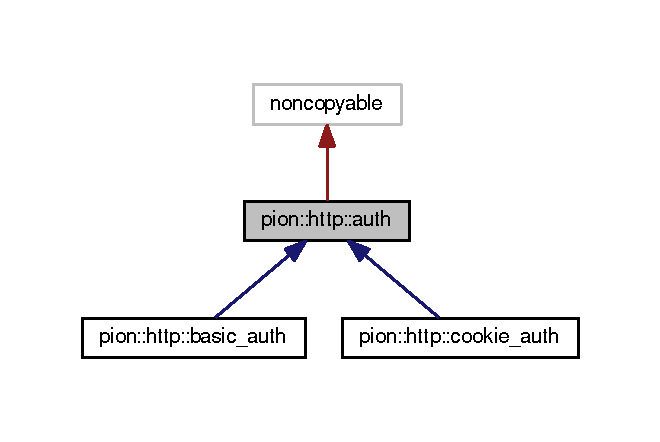
\includegraphics[width=317pt]{classpion_1_1http_1_1auth__inherit__graph}
\end{center}
\end{figure}


Collaboration diagram for pion\-:\-:http\-:\-:auth\-:
\nopagebreak
\begin{figure}[H]
\begin{center}
\leavevmode
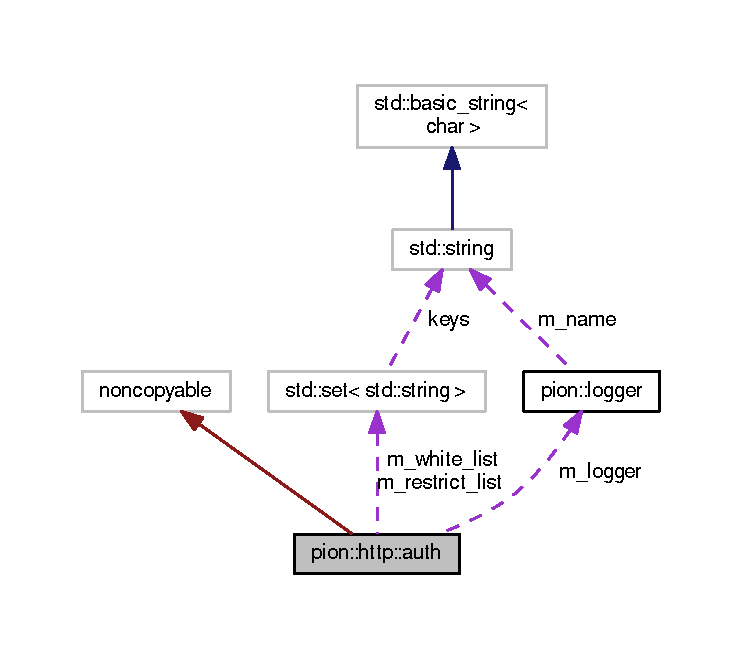
\includegraphics[width=350pt]{classpion_1_1http_1_1auth__coll__graph}
\end{center}
\end{figure}
\subsection*{Public Member Functions}
\begin{DoxyCompactItemize}
\item 
\hyperlink{classpion_1_1http_1_1auth_a464d923e5f67955ae6862f749ea79cd7}{auth} (\hyperlink{namespacepion_a20602680730b88b8efd08b3730d601af}{user\-\_\-manager\-\_\-ptr} user\-Manager)
\begin{DoxyCompactList}\small\item\em default constructor \end{DoxyCompactList}\item 
virtual \hyperlink{classpion_1_1http_1_1auth_a8e58182470ebd406f5754064a890786c}{$\sim$auth} ()
\begin{DoxyCompactList}\small\item\em virtual destructor \end{DoxyCompactList}\item 
virtual bool \hyperlink{classpion_1_1http_1_1auth_ad59da7a2c24929b7dd4d41c5679bb8bf}{handle\-\_\-request} (const \hyperlink{namespacepion_1_1http_ace432b70a9459d50ff4969a7a47f0ccb}{http\-::request\-\_\-ptr} \&http\-\_\-request\-\_\-ptr, const \hyperlink{namespacepion_1_1tcp_a6c9b7497068009f6d81d95ec0b0627d6}{tcp\-::connection\-\_\-ptr} \&tcp\-\_\-conn)=0
\item 
virtual void \hyperlink{classpion_1_1http_1_1auth_a49861152e006dc35880152ed0e7a6e92}{set\-\_\-option} (const std\-::string \&name, const std\-::string \&)
\item 
void \hyperlink{classpion_1_1http_1_1auth_a4f3dee0db0f53e8c78a24970fcd920ea}{add\-\_\-restrict} (const std\-::string \&resource)
\item 
void \hyperlink{classpion_1_1http_1_1auth_a915cab76915bb3140007d4a432f881ce}{add\-\_\-permit} (const std\-::string \&resource)
\item 
virtual bool \hyperlink{classpion_1_1http_1_1auth_a5d2af1bf25e6e3342cafe8b1f2cf9df9}{add\-\_\-user} (std\-::string const \&username, std\-::string const \&password)
\item 
virtual bool \hyperlink{classpion_1_1http_1_1auth_a850f65087e873e31de22b0a0fef79232}{update\-\_\-user} (std\-::string const \&username, std\-::string const \&password)
\item 
virtual bool \hyperlink{classpion_1_1http_1_1auth_a5bb4dce624e8cfe416951bbed3ddce43}{remove\-\_\-user} (std\-::string const \&username)
\item 
virtual \hyperlink{namespacepion_afd2ae32f926db1286ba2e83011456e11}{user\-\_\-ptr} \hyperlink{classpion_1_1http_1_1auth_aa066cc49589f0629b5b6e2a0e7050516}{get\-\_\-user} (std\-::string const \&username)
\end{DoxyCompactItemize}
\subsection*{Protected Types}
\begin{DoxyCompactItemize}
\item 
typedef std\-::set$<$ std\-::string $>$ \hyperlink{classpion_1_1http_1_1auth_afba7081a3795e3010f0051e4e85a38e3}{resource\-\_\-set\-\_\-type}
\begin{DoxyCompactList}\small\item\em data type for a set of resources to be authenticated \end{DoxyCompactList}\item 
typedef std\-::map$<$ std\-::string, \\*
std\-::pair\\*
$<$ boost\-::posix\-\_\-time\-::ptime, \\*
\hyperlink{namespacepion_afd2ae32f926db1286ba2e83011456e11}{user\-\_\-ptr} $>$ $>$ \hyperlink{classpion_1_1http_1_1auth_a57a2002495d45ac3ea508ee4186356b5}{user\-\_\-cache\-\_\-type}
\begin{DoxyCompactList}\small\item\em data type used to map authentication credentials to user objects \end{DoxyCompactList}\end{DoxyCompactItemize}
\subsection*{Protected Member Functions}
\begin{DoxyCompactItemize}
\item 
bool \hyperlink{classpion_1_1http_1_1auth_a62f9ddca03be608b7884542b0d6904f6}{need\-\_\-authentication} (\hyperlink{namespacepion_1_1http_ace432b70a9459d50ff4969a7a47f0ccb}{http\-::request\-\_\-ptr} const \&http\-\_\-request\-\_\-ptr) const 
\item 
bool \hyperlink{classpion_1_1http_1_1auth_a87046c8b7fe4b74b1b76704c2093f6a9}{find\-\_\-resource} (const \hyperlink{classpion_1_1http_1_1auth_afba7081a3795e3010f0051e4e85a38e3}{resource\-\_\-set\-\_\-type} \&resource\-\_\-set, const std\-::string \&resource) const 
\item 
void \hyperlink{classpion_1_1http_1_1auth_af25a5d74ab812554d6c04379c856d019}{set\-\_\-logger} (\hyperlink{structpion_1_1logger}{logger} log\-\_\-ptr)
\begin{DoxyCompactList}\small\item\em sets the logger to be used \end{DoxyCompactList}\end{DoxyCompactItemize}
\subsection*{Protected Attributes}
\begin{DoxyCompactItemize}
\item 
\hyperlink{structpion_1_1logger}{logger} \hyperlink{classpion_1_1http_1_1auth_a936282ab441711ea3c5e52eab6ac9948}{m\-\_\-logger}
\begin{DoxyCompactList}\small\item\em primary logging interface used by this class \end{DoxyCompactList}\item 
\hyperlink{namespacepion_a20602680730b88b8efd08b3730d601af}{user\-\_\-manager\-\_\-ptr} \hyperlink{classpion_1_1http_1_1auth_a5f85a718dc74306a6f62c931d2b4bc53}{m\-\_\-user\-\_\-manager}
\begin{DoxyCompactList}\small\item\em container used to manager user objects \end{DoxyCompactList}\item 
\hyperlink{classpion_1_1http_1_1auth_afba7081a3795e3010f0051e4e85a38e3}{resource\-\_\-set\-\_\-type} \hyperlink{classpion_1_1http_1_1auth_a39970188567b9719e779dfe9ec0c901b}{m\-\_\-restrict\-\_\-list}
\begin{DoxyCompactList}\small\item\em collection of resources that require authentication \end{DoxyCompactList}\item 
\hyperlink{classpion_1_1http_1_1auth_afba7081a3795e3010f0051e4e85a38e3}{resource\-\_\-set\-\_\-type} \hyperlink{classpion_1_1http_1_1auth_a7c65c43c168549ae65ce443c10a9021a}{m\-\_\-white\-\_\-list}
\begin{DoxyCompactList}\small\item\em collection of resources that do N\-O\-T require authentication \end{DoxyCompactList}\item 
boost\-::mutex \hyperlink{classpion_1_1http_1_1auth_a5c1e57d2531c833a747ebbf9f3efe213}{m\-\_\-resource\-\_\-mutex}
\begin{DoxyCompactList}\small\item\em mutex used to protect access to the resources \end{DoxyCompactList}\end{DoxyCompactItemize}


\subsection{Detailed Description}
auth\-: a base class for handling H\-T\-T\-P Authentication and session management 

\subsection{Member Typedef Documentation}
\hypertarget{classpion_1_1http_1_1auth_afba7081a3795e3010f0051e4e85a38e3}{\index{pion\-::http\-::auth@{pion\-::http\-::auth}!resource\-\_\-set\-\_\-type@{resource\-\_\-set\-\_\-type}}
\index{resource\-\_\-set\-\_\-type@{resource\-\_\-set\-\_\-type}!pion::http::auth@{pion\-::http\-::auth}}
\subsubsection[{resource\-\_\-set\-\_\-type}]{\setlength{\rightskip}{0pt plus 5cm}typedef std\-::set$<$std\-::string$>$ {\bf pion\-::http\-::auth\-::resource\-\_\-set\-\_\-type}\hspace{0.3cm}{\ttfamily [protected]}}}\label{classpion_1_1http_1_1auth_afba7081a3795e3010f0051e4e85a38e3}


data type for a set of resources to be authenticated 

\hypertarget{classpion_1_1http_1_1auth_a57a2002495d45ac3ea508ee4186356b5}{\index{pion\-::http\-::auth@{pion\-::http\-::auth}!user\-\_\-cache\-\_\-type@{user\-\_\-cache\-\_\-type}}
\index{user\-\_\-cache\-\_\-type@{user\-\_\-cache\-\_\-type}!pion::http::auth@{pion\-::http\-::auth}}
\subsubsection[{user\-\_\-cache\-\_\-type}]{\setlength{\rightskip}{0pt plus 5cm}typedef std\-::map$<$std\-::string,std\-::pair$<$boost\-::posix\-\_\-time\-::ptime,{\bf user\-\_\-ptr}$>$ $>$ {\bf pion\-::http\-::auth\-::user\-\_\-cache\-\_\-type}\hspace{0.3cm}{\ttfamily [protected]}}}\label{classpion_1_1http_1_1auth_a57a2002495d45ac3ea508ee4186356b5}


data type used to map authentication credentials to user objects 



\subsection{Constructor \& Destructor Documentation}
\hypertarget{classpion_1_1http_1_1auth_a464d923e5f67955ae6862f749ea79cd7}{\index{pion\-::http\-::auth@{pion\-::http\-::auth}!auth@{auth}}
\index{auth@{auth}!pion::http::auth@{pion\-::http\-::auth}}
\subsubsection[{auth}]{\setlength{\rightskip}{0pt plus 5cm}pion\-::http\-::auth\-::auth (
\begin{DoxyParamCaption}
\item[{{\bf user\-\_\-manager\-\_\-ptr}}]{user\-Manager}
\end{DoxyParamCaption}
)\hspace{0.3cm}{\ttfamily [inline]}}}\label{classpion_1_1http_1_1auth_a464d923e5f67955ae6862f749ea79cd7}


default constructor 

\hypertarget{classpion_1_1http_1_1auth_a8e58182470ebd406f5754064a890786c}{\index{pion\-::http\-::auth@{pion\-::http\-::auth}!$\sim$auth@{$\sim$auth}}
\index{$\sim$auth@{$\sim$auth}!pion::http::auth@{pion\-::http\-::auth}}
\subsubsection[{$\sim$auth}]{\setlength{\rightskip}{0pt plus 5cm}virtual pion\-::http\-::auth\-::$\sim$auth (
\begin{DoxyParamCaption}
{}
\end{DoxyParamCaption}
)\hspace{0.3cm}{\ttfamily [inline]}, {\ttfamily [virtual]}}}\label{classpion_1_1http_1_1auth_a8e58182470ebd406f5754064a890786c}


virtual destructor 



\subsection{Member Function Documentation}
\hypertarget{classpion_1_1http_1_1auth_a915cab76915bb3140007d4a432f881ce}{\index{pion\-::http\-::auth@{pion\-::http\-::auth}!add\-\_\-permit@{add\-\_\-permit}}
\index{add\-\_\-permit@{add\-\_\-permit}!pion::http::auth@{pion\-::http\-::auth}}
\subsubsection[{add\-\_\-permit}]{\setlength{\rightskip}{0pt plus 5cm}void pion\-::http\-::auth\-::add\-\_\-permit (
\begin{DoxyParamCaption}
\item[{const std\-::string \&}]{resource}
\end{DoxyParamCaption}
)}}\label{classpion_1_1http_1_1auth_a915cab76915bb3140007d4a432f881ce}
adds a resource that does N\-O\-T require authentication


\begin{DoxyParams}{Parameters}
{\em resource} & the resource name or uri-\/stem that does not require authentication \\
\hline
\end{DoxyParams}


References m\-\_\-logger, m\-\_\-resource\-\_\-mutex, m\-\_\-white\-\_\-list, P\-I\-O\-N\-\_\-\-L\-O\-G\-\_\-\-I\-N\-F\-O, and pion\-::http\-::server\-::strip\-\_\-trailing\-\_\-slash().

\hypertarget{classpion_1_1http_1_1auth_a4f3dee0db0f53e8c78a24970fcd920ea}{\index{pion\-::http\-::auth@{pion\-::http\-::auth}!add\-\_\-restrict@{add\-\_\-restrict}}
\index{add\-\_\-restrict@{add\-\_\-restrict}!pion::http::auth@{pion\-::http\-::auth}}
\subsubsection[{add\-\_\-restrict}]{\setlength{\rightskip}{0pt plus 5cm}void pion\-::http\-::auth\-::add\-\_\-restrict (
\begin{DoxyParamCaption}
\item[{const std\-::string \&}]{resource}
\end{DoxyParamCaption}
)}}\label{classpion_1_1http_1_1auth_a4f3dee0db0f53e8c78a24970fcd920ea}
adds a resource that requires authentication


\begin{DoxyParams}{Parameters}
{\em resource} & the resource name or uri-\/stem that requires authentication \\
\hline
\end{DoxyParams}


References m\-\_\-logger, m\-\_\-resource\-\_\-mutex, m\-\_\-restrict\-\_\-list, P\-I\-O\-N\-\_\-\-L\-O\-G\-\_\-\-I\-N\-F\-O, and pion\-::http\-::server\-::strip\-\_\-trailing\-\_\-slash().

\hypertarget{classpion_1_1http_1_1auth_a5d2af1bf25e6e3342cafe8b1f2cf9df9}{\index{pion\-::http\-::auth@{pion\-::http\-::auth}!add\-\_\-user@{add\-\_\-user}}
\index{add\-\_\-user@{add\-\_\-user}!pion::http::auth@{pion\-::http\-::auth}}
\subsubsection[{add\-\_\-user}]{\setlength{\rightskip}{0pt plus 5cm}virtual bool pion\-::http\-::auth\-::add\-\_\-user (
\begin{DoxyParamCaption}
\item[{std\-::string const \&}]{username, }
\item[{std\-::string const \&}]{password}
\end{DoxyParamCaption}
)\hspace{0.3cm}{\ttfamily [inline]}, {\ttfamily [virtual]}}}\label{classpion_1_1http_1_1auth_a5d2af1bf25e6e3342cafe8b1f2cf9df9}
used to add a new user

@ return false if user with such name already exists \hypertarget{classpion_1_1http_1_1auth_a87046c8b7fe4b74b1b76704c2093f6a9}{\index{pion\-::http\-::auth@{pion\-::http\-::auth}!find\-\_\-resource@{find\-\_\-resource}}
\index{find\-\_\-resource@{find\-\_\-resource}!pion::http::auth@{pion\-::http\-::auth}}
\subsubsection[{find\-\_\-resource}]{\setlength{\rightskip}{0pt plus 5cm}bool pion\-::http\-::auth\-::find\-\_\-resource (
\begin{DoxyParamCaption}
\item[{const {\bf resource\-\_\-set\-\_\-type} \&}]{resource\-\_\-set, }
\item[{const std\-::string \&}]{resource}
\end{DoxyParamCaption}
) const\hspace{0.3cm}{\ttfamily [protected]}}}\label{classpion_1_1http_1_1auth_a87046c8b7fe4b74b1b76704c2093f6a9}
tries to find a resource in a given collection


\begin{DoxyParams}{Parameters}
{\em resource\-\_\-set} & the collection of resource to look in \\
\hline
{\em resource} & the resource to look for\\
\hline
\end{DoxyParams}
\begin{DoxyReturn}{Returns}
true if the resource was found 
\end{DoxyReturn}


Referenced by need\-\_\-authentication().

\hypertarget{classpion_1_1http_1_1auth_aa066cc49589f0629b5b6e2a0e7050516}{\index{pion\-::http\-::auth@{pion\-::http\-::auth}!get\-\_\-user@{get\-\_\-user}}
\index{get\-\_\-user@{get\-\_\-user}!pion::http::auth@{pion\-::http\-::auth}}
\subsubsection[{get\-\_\-user}]{\setlength{\rightskip}{0pt plus 5cm}virtual {\bf user\-\_\-ptr} pion\-::http\-::auth\-::get\-\_\-user (
\begin{DoxyParamCaption}
\item[{std\-::string const \&}]{username}
\end{DoxyParamCaption}
)\hspace{0.3cm}{\ttfamily [inline]}, {\ttfamily [virtual]}}}\label{classpion_1_1http_1_1auth_aa066cc49589f0629b5b6e2a0e7050516}
Used to locate user object by username \hypertarget{classpion_1_1http_1_1auth_ad59da7a2c24929b7dd4d41c5679bb8bf}{\index{pion\-::http\-::auth@{pion\-::http\-::auth}!handle\-\_\-request@{handle\-\_\-request}}
\index{handle\-\_\-request@{handle\-\_\-request}!pion::http::auth@{pion\-::http\-::auth}}
\subsubsection[{handle\-\_\-request}]{\setlength{\rightskip}{0pt plus 5cm}virtual bool pion\-::http\-::auth\-::handle\-\_\-request (
\begin{DoxyParamCaption}
\item[{const {\bf http\-::request\-\_\-ptr} \&}]{http\-\_\-request\-\_\-ptr, }
\item[{const {\bf tcp\-::connection\-\_\-ptr} \&}]{tcp\-\_\-conn}
\end{DoxyParamCaption}
)\hspace{0.3cm}{\ttfamily [pure virtual]}}}\label{classpion_1_1http_1_1auth_ad59da7a2c24929b7dd4d41c5679bb8bf}
attempts to validate authentication of a new H\-T\-T\-P request. If request valid, pointer to user identity object (if any) will be preserved in the request and return \char`\"{}true\char`\"{}. If request not authenticated, appropriate response is sent over tcp\-\_\-conn and return \char`\"{}false\char`\"{};


\begin{DoxyParams}{Parameters}
{\em http\-\_\-request\-\_\-ptr} & the new H\-T\-T\-P request to handle \\
\hline
{\em tcp\-\_\-conn} & the T\-C\-P connection that has the new request\\
\hline
\end{DoxyParams}
\begin{DoxyReturn}{Returns}
true if request valid and user identity inserted into request 
\end{DoxyReturn}


Implemented in \hyperlink{classpion_1_1http_1_1cookie__auth_a585dc707d10e0e86ba33efdfc330c83a}{pion\-::http\-::cookie\-\_\-auth}, and \hyperlink{classpion_1_1http_1_1basic__auth_a032fb3d76e1e4f4e484a97bae7f5b367}{pion\-::http\-::basic\-\_\-auth}.

\hypertarget{classpion_1_1http_1_1auth_a62f9ddca03be608b7884542b0d6904f6}{\index{pion\-::http\-::auth@{pion\-::http\-::auth}!need\-\_\-authentication@{need\-\_\-authentication}}
\index{need\-\_\-authentication@{need\-\_\-authentication}!pion::http::auth@{pion\-::http\-::auth}}
\subsubsection[{need\-\_\-authentication}]{\setlength{\rightskip}{0pt plus 5cm}bool pion\-::http\-::auth\-::need\-\_\-authentication (
\begin{DoxyParamCaption}
\item[{{\bf http\-::request\-\_\-ptr} const \&}]{http\-\_\-request\-\_\-ptr}
\end{DoxyParamCaption}
) const\hspace{0.3cm}{\ttfamily [protected]}}}\label{classpion_1_1http_1_1auth_a62f9ddca03be608b7884542b0d6904f6}
check if given H\-T\-T\-P request requires authentication


\begin{DoxyParams}{Parameters}
{\em http\-\_\-request\-\_\-ptr} & the H\-T\-T\-P request to check \\
\hline
\end{DoxyParams}


References find\-\_\-resource(), m\-\_\-resource\-\_\-mutex, m\-\_\-restrict\-\_\-list, m\-\_\-user\-\_\-manager, m\-\_\-white\-\_\-list, and pion\-::http\-::server\-::strip\-\_\-trailing\-\_\-slash().



Referenced by pion\-::http\-::basic\-\_\-auth\-::handle\-\_\-request(), and pion\-::http\-::cookie\-\_\-auth\-::handle\-\_\-request().

\hypertarget{classpion_1_1http_1_1auth_a5bb4dce624e8cfe416951bbed3ddce43}{\index{pion\-::http\-::auth@{pion\-::http\-::auth}!remove\-\_\-user@{remove\-\_\-user}}
\index{remove\-\_\-user@{remove\-\_\-user}!pion::http::auth@{pion\-::http\-::auth}}
\subsubsection[{remove\-\_\-user}]{\setlength{\rightskip}{0pt plus 5cm}virtual bool pion\-::http\-::auth\-::remove\-\_\-user (
\begin{DoxyParamCaption}
\item[{std\-::string const \&}]{username}
\end{DoxyParamCaption}
)\hspace{0.3cm}{\ttfamily [inline]}, {\ttfamily [virtual]}}}\label{classpion_1_1http_1_1auth_a5bb4dce624e8cfe416951bbed3ddce43}
used to remove given user

\begin{DoxyReturn}{Returns}
false if no user with such username 
\end{DoxyReturn}
\hypertarget{classpion_1_1http_1_1auth_af25a5d74ab812554d6c04379c856d019}{\index{pion\-::http\-::auth@{pion\-::http\-::auth}!set\-\_\-logger@{set\-\_\-logger}}
\index{set\-\_\-logger@{set\-\_\-logger}!pion::http::auth@{pion\-::http\-::auth}}
\subsubsection[{set\-\_\-logger}]{\setlength{\rightskip}{0pt plus 5cm}void pion\-::http\-::auth\-::set\-\_\-logger (
\begin{DoxyParamCaption}
\item[{{\bf logger}}]{log\-\_\-ptr}
\end{DoxyParamCaption}
)\hspace{0.3cm}{\ttfamily [inline]}, {\ttfamily [protected]}}}\label{classpion_1_1http_1_1auth_af25a5d74ab812554d6c04379c856d019}


sets the logger to be used 



Referenced by pion\-::http\-::basic\-\_\-auth\-::basic\-\_\-auth(), and pion\-::http\-::cookie\-\_\-auth\-::cookie\-\_\-auth().

\hypertarget{classpion_1_1http_1_1auth_a49861152e006dc35880152ed0e7a6e92}{\index{pion\-::http\-::auth@{pion\-::http\-::auth}!set\-\_\-option@{set\-\_\-option}}
\index{set\-\_\-option@{set\-\_\-option}!pion::http::auth@{pion\-::http\-::auth}}
\subsubsection[{set\-\_\-option}]{\setlength{\rightskip}{0pt plus 5cm}virtual void pion\-::http\-::auth\-::set\-\_\-option (
\begin{DoxyParamCaption}
\item[{const std\-::string \&}]{name, }
\item[{const std\-::string \&}]{}
\end{DoxyParamCaption}
)\hspace{0.3cm}{\ttfamily [inline]}, {\ttfamily [virtual]}}}\label{classpion_1_1http_1_1auth_a49861152e006dc35880152ed0e7a6e92}
sets a configuration option


\begin{DoxyParams}{Parameters}
{\em name} & the name of the option to change \\
\hline
{\em value} & the value of the option \\
\hline
\end{DoxyParams}


Reimplemented in \hyperlink{classpion_1_1http_1_1cookie__auth_a87eb9ebf16f524aaf672465c37299772}{pion\-::http\-::cookie\-\_\-auth}, and \hyperlink{classpion_1_1http_1_1basic__auth_a9da335bd02b00b82cff40cb333fe7ee7}{pion\-::http\-::basic\-\_\-auth}.

\hypertarget{classpion_1_1http_1_1auth_a850f65087e873e31de22b0a0fef79232}{\index{pion\-::http\-::auth@{pion\-::http\-::auth}!update\-\_\-user@{update\-\_\-user}}
\index{update\-\_\-user@{update\-\_\-user}!pion::http::auth@{pion\-::http\-::auth}}
\subsubsection[{update\-\_\-user}]{\setlength{\rightskip}{0pt plus 5cm}virtual bool pion\-::http\-::auth\-::update\-\_\-user (
\begin{DoxyParamCaption}
\item[{std\-::string const \&}]{username, }
\item[{std\-::string const \&}]{password}
\end{DoxyParamCaption}
)\hspace{0.3cm}{\ttfamily [inline]}, {\ttfamily [virtual]}}}\label{classpion_1_1http_1_1auth_a850f65087e873e31de22b0a0fef79232}
update password for given user

\begin{DoxyReturn}{Returns}
false if user with such a name doesn't exist 
\end{DoxyReturn}


\subsection{Member Data Documentation}
\hypertarget{classpion_1_1http_1_1auth_a936282ab441711ea3c5e52eab6ac9948}{\index{pion\-::http\-::auth@{pion\-::http\-::auth}!m\-\_\-logger@{m\-\_\-logger}}
\index{m\-\_\-logger@{m\-\_\-logger}!pion::http::auth@{pion\-::http\-::auth}}
\subsubsection[{m\-\_\-logger}]{\setlength{\rightskip}{0pt plus 5cm}{\bf logger} pion\-::http\-::auth\-::m\-\_\-logger\hspace{0.3cm}{\ttfamily [mutable]}, {\ttfamily [protected]}}}\label{classpion_1_1http_1_1auth_a936282ab441711ea3c5e52eab6ac9948}


primary logging interface used by this class 



Referenced by add\-\_\-permit(), and add\-\_\-restrict().

\hypertarget{classpion_1_1http_1_1auth_a5c1e57d2531c833a747ebbf9f3efe213}{\index{pion\-::http\-::auth@{pion\-::http\-::auth}!m\-\_\-resource\-\_\-mutex@{m\-\_\-resource\-\_\-mutex}}
\index{m\-\_\-resource\-\_\-mutex@{m\-\_\-resource\-\_\-mutex}!pion::http::auth@{pion\-::http\-::auth}}
\subsubsection[{m\-\_\-resource\-\_\-mutex}]{\setlength{\rightskip}{0pt plus 5cm}boost\-::mutex pion\-::http\-::auth\-::m\-\_\-resource\-\_\-mutex\hspace{0.3cm}{\ttfamily [mutable]}, {\ttfamily [protected]}}}\label{classpion_1_1http_1_1auth_a5c1e57d2531c833a747ebbf9f3efe213}


mutex used to protect access to the resources 



Referenced by add\-\_\-permit(), add\-\_\-restrict(), and need\-\_\-authentication().

\hypertarget{classpion_1_1http_1_1auth_a39970188567b9719e779dfe9ec0c901b}{\index{pion\-::http\-::auth@{pion\-::http\-::auth}!m\-\_\-restrict\-\_\-list@{m\-\_\-restrict\-\_\-list}}
\index{m\-\_\-restrict\-\_\-list@{m\-\_\-restrict\-\_\-list}!pion::http::auth@{pion\-::http\-::auth}}
\subsubsection[{m\-\_\-restrict\-\_\-list}]{\setlength{\rightskip}{0pt plus 5cm}{\bf resource\-\_\-set\-\_\-type} pion\-::http\-::auth\-::m\-\_\-restrict\-\_\-list\hspace{0.3cm}{\ttfamily [protected]}}}\label{classpion_1_1http_1_1auth_a39970188567b9719e779dfe9ec0c901b}


collection of resources that require authentication 



Referenced by add\-\_\-restrict(), and need\-\_\-authentication().

\hypertarget{classpion_1_1http_1_1auth_a5f85a718dc74306a6f62c931d2b4bc53}{\index{pion\-::http\-::auth@{pion\-::http\-::auth}!m\-\_\-user\-\_\-manager@{m\-\_\-user\-\_\-manager}}
\index{m\-\_\-user\-\_\-manager@{m\-\_\-user\-\_\-manager}!pion::http::auth@{pion\-::http\-::auth}}
\subsubsection[{m\-\_\-user\-\_\-manager}]{\setlength{\rightskip}{0pt plus 5cm}{\bf user\-\_\-manager\-\_\-ptr} pion\-::http\-::auth\-::m\-\_\-user\-\_\-manager\hspace{0.3cm}{\ttfamily [protected]}}}\label{classpion_1_1http_1_1auth_a5f85a718dc74306a6f62c931d2b4bc53}


container used to manager user objects 



Referenced by pion\-::http\-::basic\-\_\-auth\-::handle\-\_\-request(), need\-\_\-authentication(), and pion\-::http\-::cookie\-\_\-auth\-::process\-\_\-login().

\hypertarget{classpion_1_1http_1_1auth_a7c65c43c168549ae65ce443c10a9021a}{\index{pion\-::http\-::auth@{pion\-::http\-::auth}!m\-\_\-white\-\_\-list@{m\-\_\-white\-\_\-list}}
\index{m\-\_\-white\-\_\-list@{m\-\_\-white\-\_\-list}!pion::http::auth@{pion\-::http\-::auth}}
\subsubsection[{m\-\_\-white\-\_\-list}]{\setlength{\rightskip}{0pt plus 5cm}{\bf resource\-\_\-set\-\_\-type} pion\-::http\-::auth\-::m\-\_\-white\-\_\-list\hspace{0.3cm}{\ttfamily [protected]}}}\label{classpion_1_1http_1_1auth_a7c65c43c168549ae65ce443c10a9021a}


collection of resources that do N\-O\-T require authentication 



Referenced by add\-\_\-permit(), and need\-\_\-authentication().



The documentation for this class was generated from the following files\-:\begin{DoxyCompactItemize}
\item 
include/pion/http/\hyperlink{auth_8hpp}{auth.\-hpp}\item 
src/\hyperlink{http__auth_8cpp}{http\-\_\-auth.\-cpp}\end{DoxyCompactItemize}

\hypertarget{classpion_1_1error_1_1bad__arg}{\section{pion\-:\-:error\-:\-:bad\-\_\-arg Class Reference}
\label{classpion_1_1error_1_1bad__arg}\index{pion\-::error\-::bad\-\_\-arg@{pion\-::error\-::bad\-\_\-arg}}
}


exception thrown for an invalid configuration argument or option  




{\ttfamily \#include $<$error.\-hpp$>$}



Inheritance diagram for pion\-:\-:error\-:\-:bad\-\_\-arg\-:
\nopagebreak
\begin{figure}[H]
\begin{center}
\leavevmode
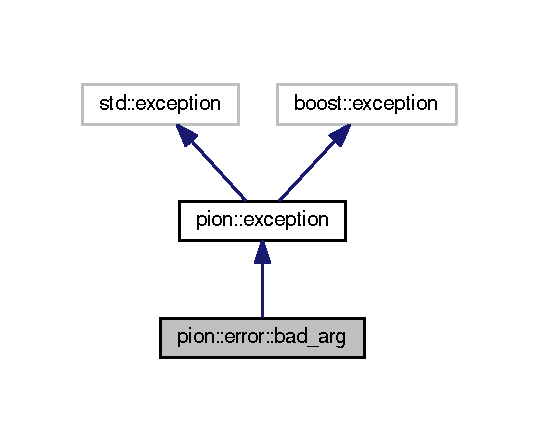
\includegraphics[width=259pt]{classpion_1_1error_1_1bad__arg__inherit__graph}
\end{center}
\end{figure}


Collaboration diagram for pion\-:\-:error\-:\-:bad\-\_\-arg\-:
\nopagebreak
\begin{figure}[H]
\begin{center}
\leavevmode
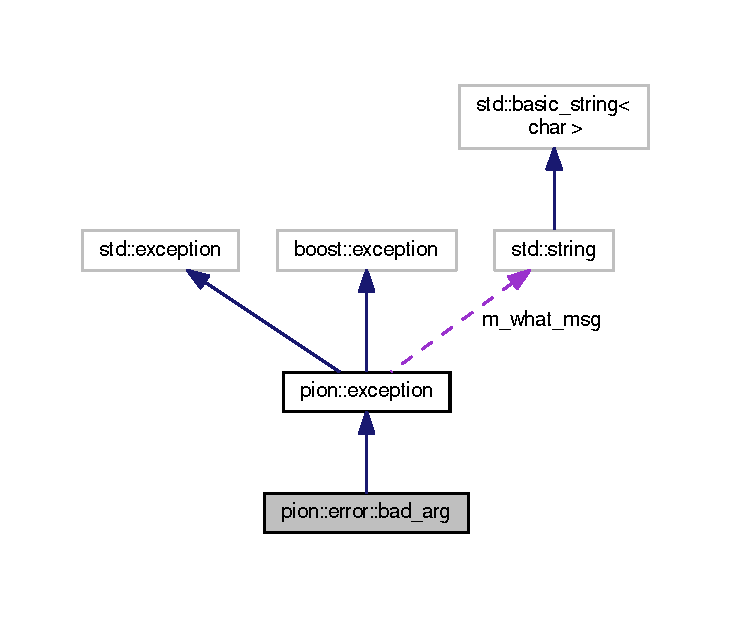
\includegraphics[width=350pt]{classpion_1_1error_1_1bad__arg__coll__graph}
\end{center}
\end{figure}
\subsection*{Additional Inherited Members}


\subsection{Detailed Description}
exception thrown for an invalid configuration argument or option 

The documentation for this class was generated from the following file\-:\begin{DoxyCompactItemize}
\item 
include/pion/\hyperlink{error_8hpp}{error.\-hpp}\end{DoxyCompactItemize}

\hypertarget{classpion_1_1error_1_1bad__config}{\section{pion\-:\-:error\-:\-:bad\-\_\-config Class Reference}
\label{classpion_1_1error_1_1bad__config}\index{pion\-::error\-::bad\-\_\-config@{pion\-::error\-::bad\-\_\-config}}
}


exception thrown if there is an error parsing a configuration file  




{\ttfamily \#include $<$error.\-hpp$>$}



Inheritance diagram for pion\-:\-:error\-:\-:bad\-\_\-config\-:
\nopagebreak
\begin{figure}[H]
\begin{center}
\leavevmode
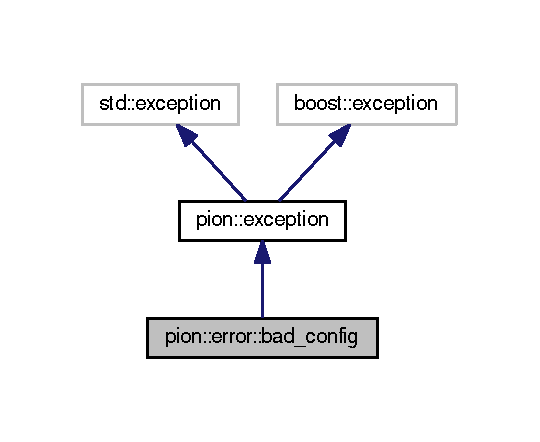
\includegraphics[width=259pt]{classpion_1_1error_1_1bad__config__inherit__graph}
\end{center}
\end{figure}


Collaboration diagram for pion\-:\-:error\-:\-:bad\-\_\-config\-:
\nopagebreak
\begin{figure}[H]
\begin{center}
\leavevmode
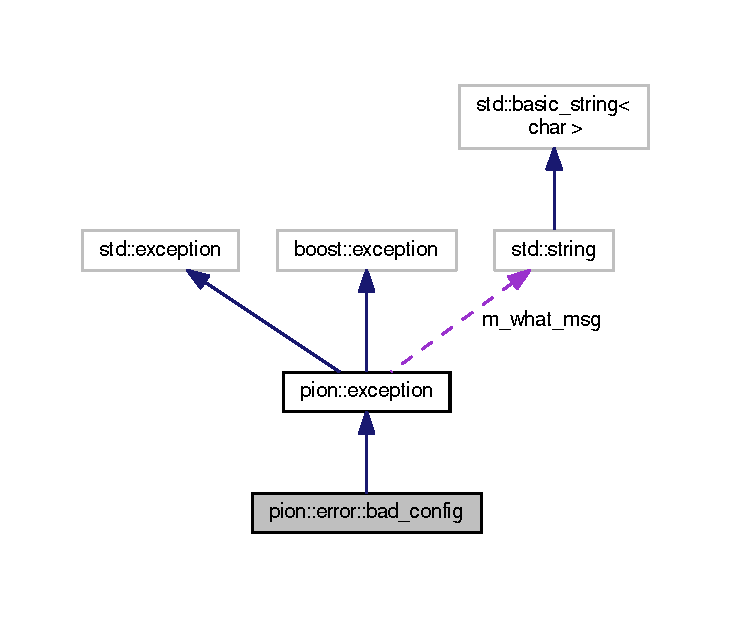
\includegraphics[width=350pt]{classpion_1_1error_1_1bad__config__coll__graph}
\end{center}
\end{figure}
\subsection*{Additional Inherited Members}


\subsection{Detailed Description}
exception thrown if there is an error parsing a configuration file 

The documentation for this class was generated from the following file\-:\begin{DoxyCompactItemize}
\item 
include/pion/\hyperlink{error_8hpp}{error.\-hpp}\end{DoxyCompactItemize}

\hypertarget{classpion_1_1error_1_1bad__password__hash}{\section{pion\-:\-:error\-:\-:bad\-\_\-password\-\_\-hash Class Reference}
\label{classpion_1_1error_1_1bad__password__hash}\index{pion\-::error\-::bad\-\_\-password\-\_\-hash@{pion\-::error\-::bad\-\_\-password\-\_\-hash}}
}


exception thrown if a bad password hash is provided  




{\ttfamily \#include $<$error.\-hpp$>$}



Inheritance diagram for pion\-:\-:error\-:\-:bad\-\_\-password\-\_\-hash\-:
\nopagebreak
\begin{figure}[H]
\begin{center}
\leavevmode
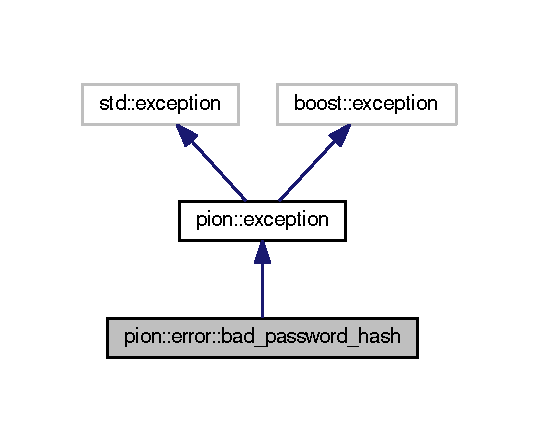
\includegraphics[width=259pt]{classpion_1_1error_1_1bad__password__hash__inherit__graph}
\end{center}
\end{figure}


Collaboration diagram for pion\-:\-:error\-:\-:bad\-\_\-password\-\_\-hash\-:
\nopagebreak
\begin{figure}[H]
\begin{center}
\leavevmode
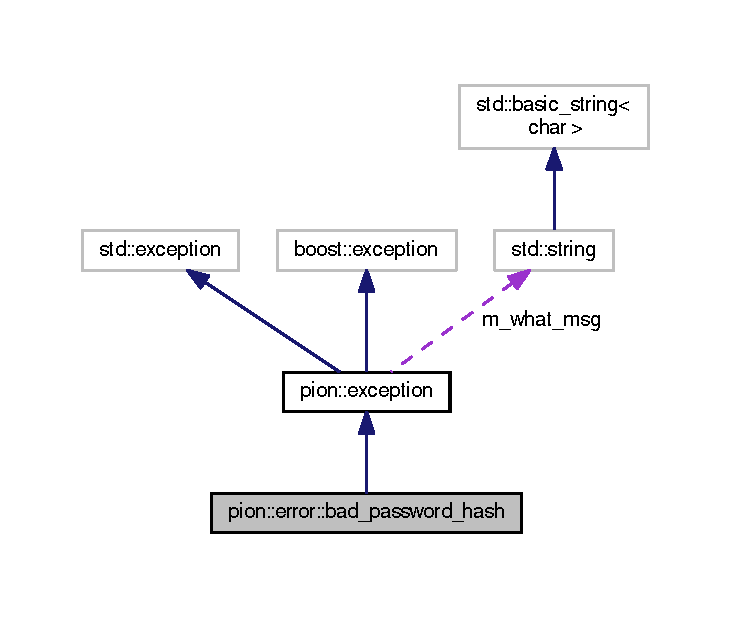
\includegraphics[width=350pt]{classpion_1_1error_1_1bad__password__hash__coll__graph}
\end{center}
\end{figure}
\subsection*{Additional Inherited Members}


\subsection{Detailed Description}
exception thrown if a bad password hash is provided 

The documentation for this class was generated from the following file\-:\begin{DoxyCompactItemize}
\item 
include/pion/\hyperlink{error_8hpp}{error.\-hpp}\end{DoxyCompactItemize}

\hypertarget{classpion_1_1http_1_1basic__auth}{\section{pion\-:\-:http\-:\-:basic\-\_\-auth Class Reference}
\label{classpion_1_1http_1_1basic__auth}\index{pion\-::http\-::basic\-\_\-auth@{pion\-::http\-::basic\-\_\-auth}}
}


{\ttfamily \#include $<$basic\-\_\-auth.\-hpp$>$}



Inheritance diagram for pion\-:\-:http\-:\-:basic\-\_\-auth\-:
\nopagebreak
\begin{figure}[H]
\begin{center}
\leavevmode
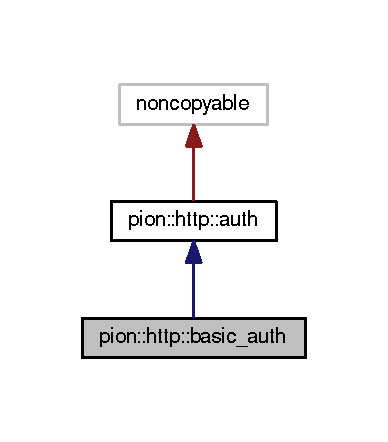
\includegraphics[width=186pt]{classpion_1_1http_1_1basic__auth__inherit__graph}
\end{center}
\end{figure}


Collaboration diagram for pion\-:\-:http\-:\-:basic\-\_\-auth\-:
\nopagebreak
\begin{figure}[H]
\begin{center}
\leavevmode
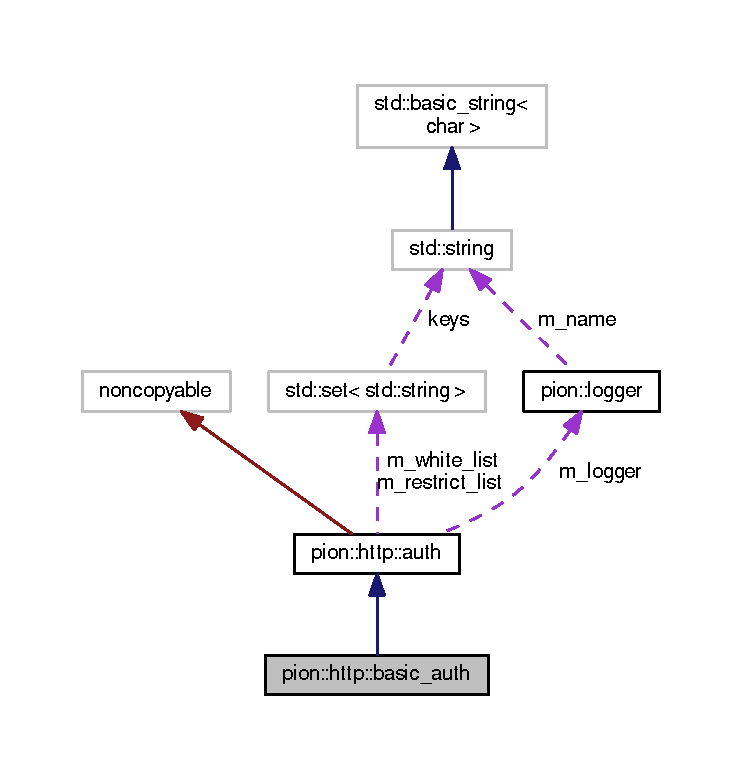
\includegraphics[width=350pt]{classpion_1_1http_1_1basic__auth__coll__graph}
\end{center}
\end{figure}
\subsection*{Public Member Functions}
\begin{DoxyCompactItemize}
\item 
\hyperlink{classpion_1_1http_1_1basic__auth_a81644f280b0c499a06e0d44bccc83773}{basic\-\_\-auth} (\hyperlink{namespacepion_a20602680730b88b8efd08b3730d601af}{user\-\_\-manager\-\_\-ptr} user\-Manager, const std\-::string \&realm=\char`\"{}P\-I\-O\-N\char`\"{})
\begin{DoxyCompactList}\small\item\em default constructor \end{DoxyCompactList}\item 
virtual \hyperlink{classpion_1_1http_1_1basic__auth_a27a464fec905b9f071d1ecb3c026709b}{$\sim$basic\-\_\-auth} ()
\begin{DoxyCompactList}\small\item\em virtual destructor \end{DoxyCompactList}\item 
virtual bool \hyperlink{classpion_1_1http_1_1basic__auth_a032fb3d76e1e4f4e484a97bae7f5b367}{handle\-\_\-request} (const \hyperlink{namespacepion_1_1http_ace432b70a9459d50ff4969a7a47f0ccb}{http\-::request\-\_\-ptr} \&http\-\_\-request\-\_\-ptr, const \hyperlink{namespacepion_1_1tcp_a6c9b7497068009f6d81d95ec0b0627d6}{tcp\-::connection\-\_\-ptr} \&tcp\-\_\-conn)
\item 
virtual void \hyperlink{classpion_1_1http_1_1basic__auth_a9da335bd02b00b82cff40cb333fe7ee7}{set\-\_\-option} (const std\-::string \&name, const std\-::string \&value)
\end{DoxyCompactItemize}
\subsection*{Protected Member Functions}
\begin{DoxyCompactItemize}
\item 
void \hyperlink{classpion_1_1http_1_1basic__auth_ac8e9633bc2e16b21a564845ede483027}{handle\-\_\-unauthorized} (const \hyperlink{namespacepion_1_1http_ace432b70a9459d50ff4969a7a47f0ccb}{http\-::request\-\_\-ptr} \&http\-\_\-request\-\_\-ptr, const \hyperlink{namespacepion_1_1tcp_a6c9b7497068009f6d81d95ec0b0627d6}{tcp\-::connection\-\_\-ptr} \&tcp\-\_\-conn)
\end{DoxyCompactItemize}
\subsection*{Static Protected Member Functions}
\begin{DoxyCompactItemize}
\item 
static bool \hyperlink{classpion_1_1http_1_1basic__auth_ae93865f8cdee463b021a8746aa802026}{parse\-\_\-authorization} (std\-::string const \&authorization, std\-::string \&credentials)
\item 
static bool \hyperlink{classpion_1_1http_1_1basic__auth_a54f121e4a3385e44d9503bc3cb9f3385}{parse\-\_\-credentials} (std\-::string const \&credentials, std\-::string \&username, std\-::string \&password)
\end{DoxyCompactItemize}
\subsection*{Additional Inherited Members}


\subsection{Detailed Description}
\hyperlink{classpion_1_1http_1_1basic__auth}{basic\-\_\-auth}\-: a base class for handling H\-T\-T\-P Authentication and session management in accordance with R\-F\-C 2617 \href{http://tools.ietf.org/html/rfc2617}{\tt http\-://tools.\-ietf.\-org/html/rfc2617} 

\subsection{Constructor \& Destructor Documentation}
\hypertarget{classpion_1_1http_1_1basic__auth_a81644f280b0c499a06e0d44bccc83773}{\index{pion\-::http\-::basic\-\_\-auth@{pion\-::http\-::basic\-\_\-auth}!basic\-\_\-auth@{basic\-\_\-auth}}
\index{basic\-\_\-auth@{basic\-\_\-auth}!pion::http::basic_auth@{pion\-::http\-::basic\-\_\-auth}}
\subsubsection[{basic\-\_\-auth}]{\setlength{\rightskip}{0pt plus 5cm}pion\-::http\-::basic\-\_\-auth\-::basic\-\_\-auth (
\begin{DoxyParamCaption}
\item[{{\bf user\-\_\-manager\-\_\-ptr}}]{user\-Manager, }
\item[{const std\-::string \&}]{realm = {\ttfamily \char`\"{}PION\char`\"{}}}
\end{DoxyParamCaption}
)}}\label{classpion_1_1http_1_1basic__auth_a81644f280b0c499a06e0d44bccc83773}


default constructor 



References P\-I\-O\-N\-\_\-\-G\-E\-T\-\_\-\-L\-O\-G\-G\-E\-R, and pion\-::http\-::auth\-::set\-\_\-logger().

\hypertarget{classpion_1_1http_1_1basic__auth_a27a464fec905b9f071d1ecb3c026709b}{\index{pion\-::http\-::basic\-\_\-auth@{pion\-::http\-::basic\-\_\-auth}!$\sim$basic\-\_\-auth@{$\sim$basic\-\_\-auth}}
\index{$\sim$basic\-\_\-auth@{$\sim$basic\-\_\-auth}!pion::http::basic_auth@{pion\-::http\-::basic\-\_\-auth}}
\subsubsection[{$\sim$basic\-\_\-auth}]{\setlength{\rightskip}{0pt plus 5cm}virtual pion\-::http\-::basic\-\_\-auth\-::$\sim$basic\-\_\-auth (
\begin{DoxyParamCaption}
{}
\end{DoxyParamCaption}
)\hspace{0.3cm}{\ttfamily [inline]}, {\ttfamily [virtual]}}}\label{classpion_1_1http_1_1basic__auth_a27a464fec905b9f071d1ecb3c026709b}


virtual destructor 



\subsection{Member Function Documentation}
\hypertarget{classpion_1_1http_1_1basic__auth_a032fb3d76e1e4f4e484a97bae7f5b367}{\index{pion\-::http\-::basic\-\_\-auth@{pion\-::http\-::basic\-\_\-auth}!handle\-\_\-request@{handle\-\_\-request}}
\index{handle\-\_\-request@{handle\-\_\-request}!pion::http::basic_auth@{pion\-::http\-::basic\-\_\-auth}}
\subsubsection[{handle\-\_\-request}]{\setlength{\rightskip}{0pt plus 5cm}bool pion\-::http\-::basic\-\_\-auth\-::handle\-\_\-request (
\begin{DoxyParamCaption}
\item[{const {\bf http\-::request\-\_\-ptr} \&}]{http\-\_\-request\-\_\-ptr, }
\item[{const {\bf tcp\-::connection\-\_\-ptr} \&}]{tcp\-\_\-conn}
\end{DoxyParamCaption}
)\hspace{0.3cm}{\ttfamily [virtual]}}}\label{classpion_1_1http_1_1basic__auth_a032fb3d76e1e4f4e484a97bae7f5b367}
attempts to validate authentication of a new H\-T\-T\-P request. If request valid, pointer to user identity object (if any) will be preserved in the request and return \char`\"{}true\char`\"{}. If request not authenticated, appropriate response is sent over tcp\-\_\-conn and return \char`\"{}false\char`\"{};


\begin{DoxyParams}{Parameters}
{\em http\-\_\-request\-\_\-ptr} & the new H\-T\-T\-P request to handle \\
\hline
{\em tcp\-\_\-conn} & the T\-C\-P connection that has the new request\\
\hline
\end{DoxyParams}
\begin{DoxyReturn}{Returns}
true if request valid and user identity inserted into request 
\end{DoxyReturn}


Implements \hyperlink{classpion_1_1http_1_1auth_ad59da7a2c24929b7dd4d41c5679bb8bf}{pion\-::http\-::auth}.



References handle\-\_\-unauthorized(), pion\-::http\-::types\-::\-H\-E\-A\-D\-E\-R\-\_\-\-A\-U\-T\-H\-O\-R\-I\-Z\-A\-T\-I\-O\-N, pion\-::http\-::auth\-::m\-\_\-user\-\_\-manager, pion\-::http\-::auth\-::need\-\_\-authentication(), parse\-\_\-authorization(), and parse\-\_\-credentials().

\hypertarget{classpion_1_1http_1_1basic__auth_ac8e9633bc2e16b21a564845ede483027}{\index{pion\-::http\-::basic\-\_\-auth@{pion\-::http\-::basic\-\_\-auth}!handle\-\_\-unauthorized@{handle\-\_\-unauthorized}}
\index{handle\-\_\-unauthorized@{handle\-\_\-unauthorized}!pion::http::basic_auth@{pion\-::http\-::basic\-\_\-auth}}
\subsubsection[{handle\-\_\-unauthorized}]{\setlength{\rightskip}{0pt plus 5cm}void pion\-::http\-::basic\-\_\-auth\-::handle\-\_\-unauthorized (
\begin{DoxyParamCaption}
\item[{const {\bf http\-::request\-\_\-ptr} \&}]{http\-\_\-request\-\_\-ptr, }
\item[{const {\bf tcp\-::connection\-\_\-ptr} \&}]{tcp\-\_\-conn}
\end{DoxyParamCaption}
)\hspace{0.3cm}{\ttfamily [protected]}}}\label{classpion_1_1http_1_1basic__auth_ac8e9633bc2e16b21a564845ede483027}
used to send responses when access to resource is not authorized


\begin{DoxyParams}{Parameters}
{\em http\-\_\-request\-\_\-ptr} & the new H\-T\-T\-P request to handle \\
\hline
{\em tcp\-\_\-conn} & the T\-C\-P connection that has the new request \\
\hline
\end{DoxyParams}


References pion\-::http\-::response\-\_\-writer\-::create(), pion\-::tcp\-::connection\-::finish(), pion\-::http\-::types\-::\-R\-E\-S\-P\-O\-N\-S\-E\-\_\-\-C\-O\-D\-E\-\_\-\-U\-N\-A\-U\-T\-H\-O\-R\-I\-Z\-E\-D, and pion\-::http\-::types\-::\-R\-E\-S\-P\-O\-N\-S\-E\-\_\-\-M\-E\-S\-S\-A\-G\-E\-\_\-\-U\-N\-A\-U\-T\-H\-O\-R\-I\-Z\-E\-D.



Referenced by handle\-\_\-request().

\hypertarget{classpion_1_1http_1_1basic__auth_ae93865f8cdee463b021a8746aa802026}{\index{pion\-::http\-::basic\-\_\-auth@{pion\-::http\-::basic\-\_\-auth}!parse\-\_\-authorization@{parse\-\_\-authorization}}
\index{parse\-\_\-authorization@{parse\-\_\-authorization}!pion::http::basic_auth@{pion\-::http\-::basic\-\_\-auth}}
\subsubsection[{parse\-\_\-authorization}]{\setlength{\rightskip}{0pt plus 5cm}bool pion\-::http\-::basic\-\_\-auth\-::parse\-\_\-authorization (
\begin{DoxyParamCaption}
\item[{std\-::string const \&}]{authorization, }
\item[{std\-::string \&}]{credentials}
\end{DoxyParamCaption}
)\hspace{0.3cm}{\ttfamily [static]}, {\ttfamily [protected]}}}\label{classpion_1_1http_1_1basic__auth_ae93865f8cdee463b021a8746aa802026}
extracts base64 user credentials from authorization string


\begin{DoxyParams}{Parameters}
{\em authorization} & value of the H\-E\-A\-D\-E\-R\-\_\-\-A\-U\-T\-H\-O\-R\-I\-Z\-A\-T\-I\-O\-N \\
\hline
\end{DoxyParams}


Referenced by handle\-\_\-request().

\hypertarget{classpion_1_1http_1_1basic__auth_a54f121e4a3385e44d9503bc3cb9f3385}{\index{pion\-::http\-::basic\-\_\-auth@{pion\-::http\-::basic\-\_\-auth}!parse\-\_\-credentials@{parse\-\_\-credentials}}
\index{parse\-\_\-credentials@{parse\-\_\-credentials}!pion::http::basic_auth@{pion\-::http\-::basic\-\_\-auth}}
\subsubsection[{parse\-\_\-credentials}]{\setlength{\rightskip}{0pt plus 5cm}bool pion\-::http\-::basic\-\_\-auth\-::parse\-\_\-credentials (
\begin{DoxyParamCaption}
\item[{std\-::string const \&}]{credentials, }
\item[{std\-::string \&}]{username, }
\item[{std\-::string \&}]{password}
\end{DoxyParamCaption}
)\hspace{0.3cm}{\ttfamily [static]}, {\ttfamily [protected]}}}\label{classpion_1_1http_1_1basic__auth_a54f121e4a3385e44d9503bc3cb9f3385}
parse base64 credentials and extract username/password 

References pion\-::algorithm\-::base64\-\_\-decode().



Referenced by handle\-\_\-request().

\hypertarget{classpion_1_1http_1_1basic__auth_a9da335bd02b00b82cff40cb333fe7ee7}{\index{pion\-::http\-::basic\-\_\-auth@{pion\-::http\-::basic\-\_\-auth}!set\-\_\-option@{set\-\_\-option}}
\index{set\-\_\-option@{set\-\_\-option}!pion::http::basic_auth@{pion\-::http\-::basic\-\_\-auth}}
\subsubsection[{set\-\_\-option}]{\setlength{\rightskip}{0pt plus 5cm}void pion\-::http\-::basic\-\_\-auth\-::set\-\_\-option (
\begin{DoxyParamCaption}
\item[{const std\-::string \&}]{name, }
\item[{const std\-::string \&}]{value}
\end{DoxyParamCaption}
)\hspace{0.3cm}{\ttfamily [virtual]}}}\label{classpion_1_1http_1_1basic__auth_a9da335bd02b00b82cff40cb333fe7ee7}
sets a configuration option Valid options\-:
\begin{DoxyItemize}
\item \char`\"{}domain\char`\"{} -\/ name of authentication domain
\end{DoxyItemize}


\begin{DoxyParams}{Parameters}
{\em name} & the name of the option to change \\
\hline
{\em value} & the value of the option \\
\hline
\end{DoxyParams}


Reimplemented from \hyperlink{classpion_1_1http_1_1auth_a49861152e006dc35880152ed0e7a6e92}{pion\-::http\-::auth}.



The documentation for this class was generated from the following files\-:\begin{DoxyCompactItemize}
\item 
include/pion/http/\hyperlink{basic__auth_8hpp}{basic\-\_\-auth.\-hpp}\item 
src/\hyperlink{http__basic__auth_8cpp}{http\-\_\-basic\-\_\-auth.\-cpp}\end{DoxyCompactItemize}

\hypertarget{structpion_1_1test_1_1config}{\section{pion\-:\-:test\-:\-:config Struct Reference}
\label{structpion_1_1test_1_1config}\index{pion\-::test\-::config@{pion\-::test\-::config}}
}


{\ttfamily \#include $<$unit\-\_\-test.\-hpp$>$}



Collaboration diagram for pion\-:\-:test\-:\-:config\-:
\nopagebreak
\begin{figure}[H]
\begin{center}
\leavevmode
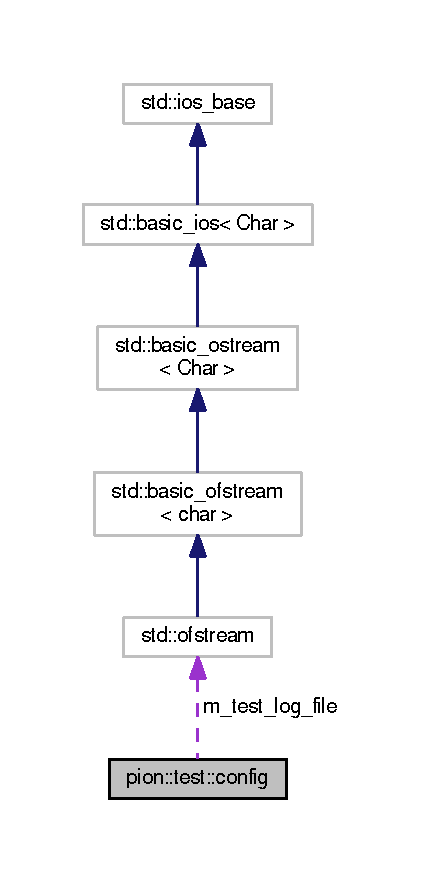
\includegraphics[width=202pt]{structpion_1_1test_1_1config__coll__graph}
\end{center}
\end{figure}
\subsection*{Public Member Functions}
\begin{DoxyCompactItemize}
\item 
\hyperlink{structpion_1_1test_1_1config_a8f6839e7c1e02c5f1a8de31290a0273c}{config} ()
\item 
virtual \hyperlink{structpion_1_1test_1_1config_a7127037d43a5f129ba6994a69308c33c}{$\sim$config} ()
\end{DoxyCompactItemize}
\subsection*{Static Public Attributes}
\begin{DoxyCompactItemize}
\item 
static std\-::ofstream \hyperlink{structpion_1_1test_1_1config_ae238691f6adbe6da8166008f70f4640a}{m\-\_\-test\-\_\-log\-\_\-file}
\begin{DoxyCompactList}\small\item\em xml log results output stream (needs to be global) \end{DoxyCompactList}\end{DoxyCompactItemize}


\subsection{Detailed Description}
config is intended for use as a global fixture. By including the following line in one source code file of a unit test project, the constructor will run once before the first test and the destructor will run once after the last test\-:

B\-O\-O\-S\-T\-\_\-\-G\-L\-O\-B\-A\-L\-\_\-\-F\-I\-X\-T\-U\-R\-E(pion\-::test\-::config); 

\subsection{Constructor \& Destructor Documentation}
\hypertarget{structpion_1_1test_1_1config_a8f6839e7c1e02c5f1a8de31290a0273c}{\index{pion\-::test\-::config@{pion\-::test\-::config}!config@{config}}
\index{config@{config}!pion::test::config@{pion\-::test\-::config}}
\subsubsection[{config}]{\setlength{\rightskip}{0pt plus 5cm}pion\-::test\-::config\-::config (
\begin{DoxyParamCaption}
{}
\end{DoxyParamCaption}
)\hspace{0.3cm}{\ttfamily [inline]}}}\label{structpion_1_1test_1_1config_a8f6839e7c1e02c5f1a8de31290a0273c}


References m\-\_\-test\-\_\-log\-\_\-file, P\-I\-O\-N\-\_\-\-G\-E\-T\-\_\-\-L\-O\-G\-G\-E\-R, P\-I\-O\-N\-\_\-\-L\-O\-G\-\_\-\-C\-O\-N\-F\-I\-G\-\_\-\-B\-A\-S\-I\-C, and P\-I\-O\-N\-\_\-\-L\-O\-G\-\_\-\-S\-E\-T\-L\-E\-V\-E\-L\-\_\-\-W\-A\-R\-N.

\hypertarget{structpion_1_1test_1_1config_a7127037d43a5f129ba6994a69308c33c}{\index{pion\-::test\-::config@{pion\-::test\-::config}!$\sim$config@{$\sim$config}}
\index{$\sim$config@{$\sim$config}!pion::test::config@{pion\-::test\-::config}}
\subsubsection[{$\sim$config}]{\setlength{\rightskip}{0pt plus 5cm}virtual pion\-::test\-::config\-::$\sim$config (
\begin{DoxyParamCaption}
{}
\end{DoxyParamCaption}
)\hspace{0.3cm}{\ttfamily [inline]}, {\ttfamily [virtual]}}}\label{structpion_1_1test_1_1config_a7127037d43a5f129ba6994a69308c33c}


\subsection{Member Data Documentation}
\hypertarget{structpion_1_1test_1_1config_ae238691f6adbe6da8166008f70f4640a}{\index{pion\-::test\-::config@{pion\-::test\-::config}!m\-\_\-test\-\_\-log\-\_\-file@{m\-\_\-test\-\_\-log\-\_\-file}}
\index{m\-\_\-test\-\_\-log\-\_\-file@{m\-\_\-test\-\_\-log\-\_\-file}!pion::test::config@{pion\-::test\-::config}}
\subsubsection[{m\-\_\-test\-\_\-log\-\_\-file}]{\setlength{\rightskip}{0pt plus 5cm}std\-::ofstream pion\-::test\-::config\-::m\-\_\-test\-\_\-log\-\_\-file\hspace{0.3cm}{\ttfamily [static]}}}\label{structpion_1_1test_1_1config_ae238691f6adbe6da8166008f70f4640a}


xml log results output stream (needs to be global) 



Referenced by config().



The documentation for this struct was generated from the following file\-:\begin{DoxyCompactItemize}
\item 
include/pion/test/\hyperlink{unit__test_8hpp}{unit\-\_\-test.\-hpp}\end{DoxyCompactItemize}

\hypertarget{structpion_1_1process_1_1config__type}{\section{pion\-:\-:process\-:\-:config\-\_\-type Struct Reference}
\label{structpion_1_1process_1_1config__type}\index{pion\-::process\-::config\-\_\-type@{pion\-::process\-::config\-\_\-type}}
}


data type for static/global process configuration information  




{\ttfamily \#include $<$process.\-hpp$>$}

\subsection*{Public Member Functions}
\begin{DoxyCompactItemize}
\item 
\hyperlink{structpion_1_1process_1_1config__type_a89ae5c8f99282b03c22006ce00c619e2}{config\-\_\-type} ()
\begin{DoxyCompactList}\small\item\em constructor just initializes native types \end{DoxyCompactList}\end{DoxyCompactItemize}
\subsection*{Public Attributes}
\begin{DoxyCompactItemize}
\item 
bool \hyperlink{structpion_1_1process_1_1config__type_aea142e63e9a962ffefb5c0d2091ed303}{shutdown\-\_\-now}
\begin{DoxyCompactList}\small\item\em true if we should shutdown now \end{DoxyCompactList}\item 
boost\-::condition \hyperlink{structpion_1_1process_1_1config__type_aec765e2fe0c8e6a474c78c2511079957}{shutdown\-\_\-cond}
\begin{DoxyCompactList}\small\item\em triggered when it is time to shutdown \end{DoxyCompactList}\item 
boost\-::mutex \hyperlink{structpion_1_1process_1_1config__type_aeea8f463fcb510add8cab8e5fa20f0e4}{shutdown\-\_\-mutex}
\begin{DoxyCompactList}\small\item\em used to protect the shutdown condition \end{DoxyCompactList}\end{DoxyCompactItemize}


\subsection{Detailed Description}
data type for static/global process configuration information 

\subsection{Constructor \& Destructor Documentation}
\hypertarget{structpion_1_1process_1_1config__type_a89ae5c8f99282b03c22006ce00c619e2}{\index{pion\-::process\-::config\-\_\-type@{pion\-::process\-::config\-\_\-type}!config\-\_\-type@{config\-\_\-type}}
\index{config\-\_\-type@{config\-\_\-type}!pion::process::config_type@{pion\-::process\-::config\-\_\-type}}
\subsubsection[{config\-\_\-type}]{\setlength{\rightskip}{0pt plus 5cm}pion\-::process\-::config\-\_\-type\-::config\-\_\-type (
\begin{DoxyParamCaption}
{}
\end{DoxyParamCaption}
)\hspace{0.3cm}{\ttfamily [inline]}}}\label{structpion_1_1process_1_1config__type_a89ae5c8f99282b03c22006ce00c619e2}


constructor just initializes native types 



\subsection{Member Data Documentation}
\hypertarget{structpion_1_1process_1_1config__type_aec765e2fe0c8e6a474c78c2511079957}{\index{pion\-::process\-::config\-\_\-type@{pion\-::process\-::config\-\_\-type}!shutdown\-\_\-cond@{shutdown\-\_\-cond}}
\index{shutdown\-\_\-cond@{shutdown\-\_\-cond}!pion::process::config_type@{pion\-::process\-::config\-\_\-type}}
\subsubsection[{shutdown\-\_\-cond}]{\setlength{\rightskip}{0pt plus 5cm}boost\-::condition pion\-::process\-::config\-\_\-type\-::shutdown\-\_\-cond}}\label{structpion_1_1process_1_1config__type_aec765e2fe0c8e6a474c78c2511079957}


triggered when it is time to shutdown 



Referenced by pion\-::process\-::shutdown(), and pion\-::process\-::wait\-\_\-for\-\_\-shutdown().

\hypertarget{structpion_1_1process_1_1config__type_aeea8f463fcb510add8cab8e5fa20f0e4}{\index{pion\-::process\-::config\-\_\-type@{pion\-::process\-::config\-\_\-type}!shutdown\-\_\-mutex@{shutdown\-\_\-mutex}}
\index{shutdown\-\_\-mutex@{shutdown\-\_\-mutex}!pion::process::config_type@{pion\-::process\-::config\-\_\-type}}
\subsubsection[{shutdown\-\_\-mutex}]{\setlength{\rightskip}{0pt plus 5cm}boost\-::mutex pion\-::process\-::config\-\_\-type\-::shutdown\-\_\-mutex}}\label{structpion_1_1process_1_1config__type_aeea8f463fcb510add8cab8e5fa20f0e4}


used to protect the shutdown condition 



Referenced by pion\-::process\-::shutdown(), and pion\-::process\-::wait\-\_\-for\-\_\-shutdown().

\hypertarget{structpion_1_1process_1_1config__type_aea142e63e9a962ffefb5c0d2091ed303}{\index{pion\-::process\-::config\-\_\-type@{pion\-::process\-::config\-\_\-type}!shutdown\-\_\-now@{shutdown\-\_\-now}}
\index{shutdown\-\_\-now@{shutdown\-\_\-now}!pion::process::config_type@{pion\-::process\-::config\-\_\-type}}
\subsubsection[{shutdown\-\_\-now}]{\setlength{\rightskip}{0pt plus 5cm}bool pion\-::process\-::config\-\_\-type\-::shutdown\-\_\-now}}\label{structpion_1_1process_1_1config__type_aea142e63e9a962ffefb5c0d2091ed303}


true if we should shutdown now 



Referenced by pion\-::process\-::shutdown(), and pion\-::process\-::wait\-\_\-for\-\_\-shutdown().



The documentation for this struct was generated from the following file\-:\begin{DoxyCompactItemize}
\item 
include/pion/\hyperlink{process_8hpp}{process.\-hpp}\end{DoxyCompactItemize}

\hypertarget{classpion_1_1tcp_1_1connection}{\section{pion\-:\-:tcp\-:\-:connection Class Reference}
\label{classpion_1_1tcp_1_1connection}\index{pion\-::tcp\-::connection@{pion\-::tcp\-::connection}}
}


{\ttfamily \#include $<$connection.\-hpp$>$}



Inheritance diagram for pion\-:\-:tcp\-:\-:connection\-:
\nopagebreak
\begin{figure}[H]
\begin{center}
\leavevmode
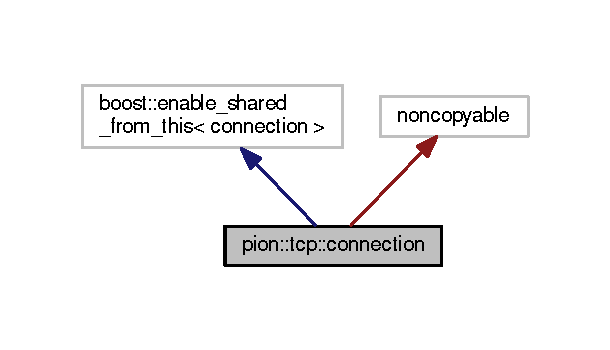
\includegraphics[width=293pt]{classpion_1_1tcp_1_1connection__inherit__graph}
\end{center}
\end{figure}


Collaboration diagram for pion\-:\-:tcp\-:\-:connection\-:
\nopagebreak
\begin{figure}[H]
\begin{center}
\leavevmode
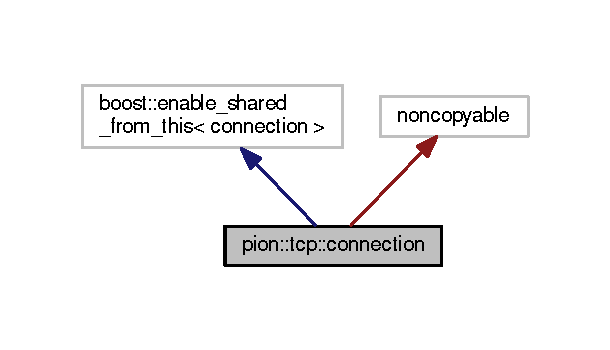
\includegraphics[width=293pt]{classpion_1_1tcp_1_1connection__coll__graph}
\end{center}
\end{figure}
\subsection*{Classes}
\begin{DoxyCompactItemize}
\item 
class \hyperlink{classpion_1_1tcp_1_1connection_1_1ssl__socket__type}{ssl\-\_\-socket\-\_\-type}
\end{DoxyCompactItemize}
\subsection*{Public Types}
\begin{DoxyCompactItemize}
\item 
enum \hyperlink{classpion_1_1tcp_1_1connection_a1888aaf31f431a3f00c70c2568f4cb25}{lifecycle\-\_\-type} \{ \hyperlink{classpion_1_1tcp_1_1connection_a1888aaf31f431a3f00c70c2568f4cb25a1eee3589ec1f6b59a13bc36fd5f48e63}{L\-I\-F\-E\-C\-Y\-C\-L\-E\-\_\-\-C\-L\-O\-S\-E}, 
\hyperlink{classpion_1_1tcp_1_1connection_a1888aaf31f431a3f00c70c2568f4cb25ab3bb67380ff48e263e16b55ff786e96f}{L\-I\-F\-E\-C\-Y\-C\-L\-E\-\_\-\-K\-E\-E\-P\-A\-L\-I\-V\-E}, 
\hyperlink{classpion_1_1tcp_1_1connection_a1888aaf31f431a3f00c70c2568f4cb25ac3e9ae9a9b7a71232679416d57b7d95f}{L\-I\-F\-E\-C\-Y\-C\-L\-E\-\_\-\-P\-I\-P\-E\-L\-I\-N\-E\-D}
 \}
\begin{DoxyCompactList}\small\item\em data type for the connection's lifecycle state \end{DoxyCompactList}\item 
enum \{ \hyperlink{classpion_1_1tcp_1_1connection_ad123ec22701e50c2c39d4a6cdbea3e92aac7c4dbea8f7fc8b471d7fcabf619221}{R\-E\-A\-D\-\_\-\-B\-U\-F\-F\-E\-R\-\_\-\-S\-I\-Z\-E} = 8192
 \}
\begin{DoxyCompactList}\small\item\em size of the read buffer \end{DoxyCompactList}\item 
typedef boost\-::function1$<$ void, \\*
boost\-::shared\-\_\-ptr$<$ \hyperlink{classpion_1_1tcp_1_1connection}{connection} $>$ $>$ \hyperlink{classpion_1_1tcp_1_1connection_aa2b220bff63f258b6aeba7eaf9a39aed}{connection\-\_\-handler}
\begin{DoxyCompactList}\small\item\em data type for a function that handles T\-C\-P connection objects \end{DoxyCompactList}\item 
typedef boost\-::array$<$ char, \\*
\hyperlink{classpion_1_1tcp_1_1connection_ad123ec22701e50c2c39d4a6cdbea3e92aac7c4dbea8f7fc8b471d7fcabf619221}{R\-E\-A\-D\-\_\-\-B\-U\-F\-F\-E\-R\-\_\-\-S\-I\-Z\-E} $>$ \hyperlink{classpion_1_1tcp_1_1connection_abd482572a19c1aecadaccd360837f7c2}{read\-\_\-buffer\-\_\-type}
\begin{DoxyCompactList}\small\item\em data type for an I/\-O read buffer \end{DoxyCompactList}\item 
typedef \\*
boost\-::asio\-::ip\-::tcp\-::socket \hyperlink{classpion_1_1tcp_1_1connection_a353c4d500505d51924d165c28b04641c}{socket\-\_\-type}
\begin{DoxyCompactList}\small\item\em data type for a socket connection \end{DoxyCompactList}\item 
typedef int \hyperlink{classpion_1_1tcp_1_1connection_a8587c35bbf48a119aa82f228e779a30e}{ssl\-\_\-context\-\_\-type}
\end{DoxyCompactItemize}
\subsection*{Public Member Functions}
\begin{DoxyCompactItemize}
\item 
\hyperlink{classpion_1_1tcp_1_1connection_a0b2f63b845ee0f7bba3c94c5fb7f567c}{connection} (boost\-::asio\-::io\-\_\-service \&io\-\_\-service, const bool ssl\-\_\-flag=false)
\item 
\hyperlink{classpion_1_1tcp_1_1connection_a33326975c04036c79e2481d6e3541c7e}{connection} (boost\-::asio\-::io\-\_\-service \&io\-\_\-service, \hyperlink{classpion_1_1tcp_1_1connection_a8587c35bbf48a119aa82f228e779a30e}{ssl\-\_\-context\-\_\-type} \&ssl\-\_\-context)
\item 
bool \hyperlink{classpion_1_1tcp_1_1connection_aa454ce0733cbd9bc97d4fe22f2eb8218}{is\-\_\-open} (void) const 
\begin{DoxyCompactList}\small\item\em returns true if the connection is currently open \end{DoxyCompactList}\item 
void \hyperlink{classpion_1_1tcp_1_1connection_a8b52fce50e8987a982c46bc82b463075}{close} (void)
\begin{DoxyCompactList}\small\item\em closes the tcp socket and cancels any pending asynchronous operations \end{DoxyCompactList}\item 
void \hyperlink{classpion_1_1tcp_1_1connection_ae0172c7e218f12a0b396a4e0e42e4de2}{cancel} (void)
\item 
virtual \hyperlink{classpion_1_1tcp_1_1connection_a4fbf93efbbb9f67dbe882c33ce3964da}{$\sim$connection} ()
\begin{DoxyCompactList}\small\item\em virtual destructor \end{DoxyCompactList}\item 
{\footnotesize template$<$typename Accept\-Handler $>$ }\\void \hyperlink{classpion_1_1tcp_1_1connection_a36dfc649870d90674938ab27feb16275}{async\-\_\-accept} (boost\-::asio\-::ip\-::tcp\-::acceptor \&tcp\-\_\-acceptor, Accept\-Handler handler)
\item 
boost\-::system\-::error\-\_\-code \hyperlink{classpion_1_1tcp_1_1connection_a5939637bc376552349938e2be4c72188}{accept} (boost\-::asio\-::ip\-::tcp\-::acceptor \&tcp\-\_\-acceptor)
\item 
{\footnotesize template$<$typename Connect\-Handler $>$ }\\void \hyperlink{classpion_1_1tcp_1_1connection_ad447a01394c31bb04b20386f4613b465}{async\-\_\-connect} (const boost\-::asio\-::ip\-::tcp\-::endpoint \&tcp\-\_\-endpoint, Connect\-Handler handler)
\item 
{\footnotesize template$<$typename Connect\-Handler $>$ }\\void \hyperlink{classpion_1_1tcp_1_1connection_ae8fe3fe2b885ff3a192e99b735ddea4c}{async\-\_\-connect} (const boost\-::asio\-::ip\-::address \&remote\-\_\-addr, const unsigned int remote\-\_\-port, Connect\-Handler handler)
\item 
boost\-::system\-::error\-\_\-code \hyperlink{classpion_1_1tcp_1_1connection_a5b183b3389ab9edfe28dbc7eaf352304}{connect} (boost\-::asio\-::ip\-::tcp\-::endpoint \&tcp\-\_\-endpoint)
\item 
boost\-::system\-::error\-\_\-code \hyperlink{classpion_1_1tcp_1_1connection_afd4930565752d4cfc1ea789ca3e87597}{connect} (const boost\-::asio\-::ip\-::address \&remote\-\_\-addr, const unsigned int remote\-\_\-port)
\item 
boost\-::system\-::error\-\_\-code \hyperlink{classpion_1_1tcp_1_1connection_ac80e46e81863a02840a25a3e2ef71b3b}{connect} (const std\-::string \&remote\-\_\-server, const unsigned int remote\-\_\-port)
\item 
{\footnotesize template$<$typename S\-S\-L\-Handshake\-Handler $>$ }\\void \hyperlink{classpion_1_1tcp_1_1connection_ab7262017bec6c8ce7dbb811d572958b5}{async\-\_\-handshake\-\_\-client} (S\-S\-L\-Handshake\-Handler handler)
\item 
{\footnotesize template$<$typename S\-S\-L\-Handshake\-Handler $>$ }\\void \hyperlink{classpion_1_1tcp_1_1connection_a177ca42941a50e49396b2ec330e251bf}{async\-\_\-handshake\-\_\-server} (S\-S\-L\-Handshake\-Handler handler)
\item 
boost\-::system\-::error\-\_\-code \hyperlink{classpion_1_1tcp_1_1connection_a09709b4bbd1a43d5902a8df0b4137f2f}{handshake\-\_\-client} (void)
\item 
boost\-::system\-::error\-\_\-code \hyperlink{classpion_1_1tcp_1_1connection_ad9306a425d685f91f6465ec8d5617931}{handshake\-\_\-server} (void)
\item 
{\footnotesize template$<$typename Read\-Handler $>$ }\\void \hyperlink{classpion_1_1tcp_1_1connection_a60d567fd754237b5bfb00004f489435f}{async\-\_\-read\-\_\-some} (Read\-Handler handler)
\item 
{\footnotesize template$<$typename Read\-Buffer\-Type , typename Read\-Handler $>$ }\\void \hyperlink{classpion_1_1tcp_1_1connection_a204ad77a69609adc435baecf29c7625e}{async\-\_\-read\-\_\-some} (Read\-Buffer\-Type read\-\_\-buffer, Read\-Handler handler)
\item 
std\-::size\-\_\-t \hyperlink{classpion_1_1tcp_1_1connection_af3c5c14c87e99bd40b605b0fb0b4a84e}{read\-\_\-some} (boost\-::system\-::error\-\_\-code \&ec)
\item 
{\footnotesize template$<$typename Read\-Buffer\-Type $>$ }\\std\-::size\-\_\-t \hyperlink{classpion_1_1tcp_1_1connection_ab0529db5feb721f55adaf8d23e6cc9c9}{read\-\_\-some} (Read\-Buffer\-Type read\-\_\-buffer, boost\-::system\-::error\-\_\-code \&ec)
\item 
{\footnotesize template$<$typename Completion\-Condition , typename Read\-Handler $>$ }\\void \hyperlink{classpion_1_1tcp_1_1connection_a6eaaee791d1093a59258b3082ef7aa60}{async\-\_\-read} (Completion\-Condition completion\-\_\-condition, Read\-Handler handler)
\item 
{\footnotesize template$<$typename Mutable\-Buffer\-Sequence , typename Completion\-Condition , typename Read\-Handler $>$ }\\void \hyperlink{classpion_1_1tcp_1_1connection_ad63926d47b0cd29b391bd8c7130719f4}{async\-\_\-read} (const Mutable\-Buffer\-Sequence \&buffers, Completion\-Condition completion\-\_\-condition, Read\-Handler handler)
\item 
{\footnotesize template$<$typename Completion\-Condition $>$ }\\std\-::size\-\_\-t \hyperlink{classpion_1_1tcp_1_1connection_aa444b18b7bc1ad8735ce021e45a3299f}{read} (Completion\-Condition completion\-\_\-condition, boost\-::system\-::error\-\_\-code \&ec)
\item 
{\footnotesize template$<$typename Mutable\-Buffer\-Sequence , typename Completion\-Condition $>$ }\\std\-::size\-\_\-t \hyperlink{classpion_1_1tcp_1_1connection_a7d1cc479b25984a53e0f218e3e48830f}{read} (const Mutable\-Buffer\-Sequence \&buffers, Completion\-Condition completion\-\_\-condition, boost\-::system\-::error\-\_\-code \&ec)
\item 
{\footnotesize template$<$typename Const\-Buffer\-Sequence , typename write\-\_\-handler\-\_\-t $>$ }\\void \hyperlink{classpion_1_1tcp_1_1connection_add2f2ab41a74476529b0e3ab3ca43ee1}{async\-\_\-write} (const Const\-Buffer\-Sequence \&buffers, write\-\_\-handler\-\_\-t handler)
\item 
{\footnotesize template$<$typename Const\-Buffer\-Sequence $>$ }\\std\-::size\-\_\-t \hyperlink{classpion_1_1tcp_1_1connection_a80f286832ed69151923837713e582709}{write} (const Const\-Buffer\-Sequence \&buffers, boost\-::system\-::error\-\_\-code \&ec)
\item 
void \hyperlink{classpion_1_1tcp_1_1connection_aa7ff7a6d8325c9cbfb026c1a441523fe}{finish} (void)
\item 
bool \hyperlink{classpion_1_1tcp_1_1connection_acf7f446c7113617abcff448fbd4ba441}{get\-\_\-ssl\-\_\-flag} (void) const 
\begin{DoxyCompactList}\small\item\em returns true if the connection is encrypted using S\-S\-L \end{DoxyCompactList}\item 
void \hyperlink{classpion_1_1tcp_1_1connection_a440cc929ced689cfe4fe4bec0620162c}{set\-\_\-lifecycle} (\hyperlink{classpion_1_1tcp_1_1connection_a1888aaf31f431a3f00c70c2568f4cb25}{lifecycle\-\_\-type} t)
\begin{DoxyCompactList}\small\item\em sets the lifecycle type for the connection \end{DoxyCompactList}\item 
\hyperlink{classpion_1_1tcp_1_1connection_a1888aaf31f431a3f00c70c2568f4cb25}{lifecycle\-\_\-type} \hyperlink{classpion_1_1tcp_1_1connection_af9000c0fa1af445375f877347de3529a}{get\-\_\-lifecycle} (void) const 
\begin{DoxyCompactList}\small\item\em returns the lifecycle type for the connection \end{DoxyCompactList}\item 
bool \hyperlink{classpion_1_1tcp_1_1connection_a35394d8c3f144ab8a264824410bb7088}{get\-\_\-keep\-\_\-alive} (void) const 
\begin{DoxyCompactList}\small\item\em returns true if the connection should be kept alive \end{DoxyCompactList}\item 
bool \hyperlink{classpion_1_1tcp_1_1connection_aa54a75a48eae812955f7ce6b2b4c3d51}{get\-\_\-pipelined} (void) const 
\begin{DoxyCompactList}\small\item\em returns true if the H\-T\-T\-P requests are pipelined \end{DoxyCompactList}\item 
\hyperlink{classpion_1_1tcp_1_1connection_abd482572a19c1aecadaccd360837f7c2}{read\-\_\-buffer\-\_\-type} \& \hyperlink{classpion_1_1tcp_1_1connection_a9ffefe15c4ae6acf85e13b315fbfc72b}{get\-\_\-read\-\_\-buffer} (void)
\begin{DoxyCompactList}\small\item\em returns the buffer used for reading data from the T\-C\-P connection \end{DoxyCompactList}\item 
void \hyperlink{classpion_1_1tcp_1_1connection_a7951ebfca8e6834faa78417c5e87a748}{save\-\_\-read\-\_\-pos} (const char $\ast$read\-\_\-ptr, const char $\ast$read\-\_\-end\-\_\-ptr)
\item 
void \hyperlink{classpion_1_1tcp_1_1connection_a4cc9d7185adda632de1f3482552ed5f6}{load\-\_\-read\-\_\-pos} (const char $\ast$\&read\-\_\-ptr, const char $\ast$\&read\-\_\-end\-\_\-ptr) const 
\item 
boost\-::asio\-::ip\-::tcp\-::endpoint \hyperlink{classpion_1_1tcp_1_1connection_a63bb4969a3816db01b1e85301ca1af91}{get\-\_\-remote\-\_\-endpoint} (void) const 
\begin{DoxyCompactList}\small\item\em returns an A\-S\-I\-O endpoint for the client connection \end{DoxyCompactList}\item 
boost\-::asio\-::ip\-::address \hyperlink{classpion_1_1tcp_1_1connection_a4863b8d10797ef101c95c660007a8c62}{get\-\_\-remote\-\_\-ip} (void) const 
\begin{DoxyCompactList}\small\item\em returns the client's I\-P address \end{DoxyCompactList}\item 
unsigned short \hyperlink{classpion_1_1tcp_1_1connection_a735bcb8b1e2a9d04ad6d12e4f0c6f5a2}{get\-\_\-remote\-\_\-port} (void) const 
\begin{DoxyCompactList}\small\item\em returns the client's port number \end{DoxyCompactList}\item 
boost\-::asio\-::io\-\_\-service \& \hyperlink{classpion_1_1tcp_1_1connection_a6bbd6e925e3389cbee18915c9d63a47f}{get\-\_\-io\-\_\-service} (void)
\begin{DoxyCompactList}\small\item\em returns reference to the io\-\_\-service used for async operations \end{DoxyCompactList}\item 
\hyperlink{classpion_1_1tcp_1_1connection_a353c4d500505d51924d165c28b04641c}{socket\-\_\-type} \& \hyperlink{classpion_1_1tcp_1_1connection_a4a237acacf373637c95d2cbd24e42e74}{get\-\_\-socket} (void)
\begin{DoxyCompactList}\small\item\em returns non-\/const reference to underlying T\-C\-P socket object \end{DoxyCompactList}\item 
\hyperlink{classpion_1_1tcp_1_1connection_1_1ssl__socket__type}{ssl\-\_\-socket\-\_\-type} \& \hyperlink{classpion_1_1tcp_1_1connection_a0f3ba6ecd1f402e1e379db5440ecda94}{get\-\_\-ssl\-\_\-socket} (void)
\begin{DoxyCompactList}\small\item\em returns non-\/const reference to underlying S\-S\-L socket object \end{DoxyCompactList}\item 
const \hyperlink{classpion_1_1tcp_1_1connection_a353c4d500505d51924d165c28b04641c}{socket\-\_\-type} \& \hyperlink{classpion_1_1tcp_1_1connection_a16cef7660bcf80131d007351defe10a5}{get\-\_\-socket} (void) const 
\begin{DoxyCompactList}\small\item\em returns const reference to underlying T\-C\-P socket object \end{DoxyCompactList}\item 
const \hyperlink{classpion_1_1tcp_1_1connection_1_1ssl__socket__type}{ssl\-\_\-socket\-\_\-type} \& \hyperlink{classpion_1_1tcp_1_1connection_a8d3d2ec0d67d53b0a5d23ba3ca00dae8}{get\-\_\-ssl\-\_\-socket} (void) const 
\begin{DoxyCompactList}\small\item\em returns const reference to underlying S\-S\-L socket object \end{DoxyCompactList}\end{DoxyCompactItemize}
\subsection*{Static Public Member Functions}
\begin{DoxyCompactItemize}
\item 
static boost\-::shared\-\_\-ptr\\*
$<$ \hyperlink{classpion_1_1tcp_1_1connection}{connection} $>$ \hyperlink{classpion_1_1tcp_1_1connection_a5e9118f2f2f31b834f04d22a058fd1eb}{create} (boost\-::asio\-::io\-\_\-service \&io\-\_\-service, \hyperlink{classpion_1_1tcp_1_1connection_a8587c35bbf48a119aa82f228e779a30e}{ssl\-\_\-context\-\_\-type} \&ssl\-\_\-context, const bool ssl\-\_\-flag, \hyperlink{classpion_1_1tcp_1_1connection_aa2b220bff63f258b6aeba7eaf9a39aed}{connection\-\_\-handler} finished\-\_\-handler)
\end{DoxyCompactItemize}
\subsection*{Protected Member Functions}
\begin{DoxyCompactItemize}
\item 
\hyperlink{classpion_1_1tcp_1_1connection_a7e1f15340d3c9e593fdd15764c50dd15}{connection} (boost\-::asio\-::io\-\_\-service \&io\-\_\-service, \hyperlink{classpion_1_1tcp_1_1connection_a8587c35bbf48a119aa82f228e779a30e}{ssl\-\_\-context\-\_\-type} \&ssl\-\_\-context, const bool ssl\-\_\-flag, \hyperlink{classpion_1_1tcp_1_1connection_aa2b220bff63f258b6aeba7eaf9a39aed}{connection\-\_\-handler} finished\-\_\-handler)
\end{DoxyCompactItemize}


\subsection{Detailed Description}
connection\-: represents a single tcp connection 

\subsection{Member Typedef Documentation}
\hypertarget{classpion_1_1tcp_1_1connection_aa2b220bff63f258b6aeba7eaf9a39aed}{\index{pion\-::tcp\-::connection@{pion\-::tcp\-::connection}!connection\-\_\-handler@{connection\-\_\-handler}}
\index{connection\-\_\-handler@{connection\-\_\-handler}!pion::tcp::connection@{pion\-::tcp\-::connection}}
\subsubsection[{connection\-\_\-handler}]{\setlength{\rightskip}{0pt plus 5cm}typedef boost\-::function1$<$void, boost\-::shared\-\_\-ptr$<${\bf connection}$>$ $>$ {\bf pion\-::tcp\-::connection\-::connection\-\_\-handler}}}\label{classpion_1_1tcp_1_1connection_aa2b220bff63f258b6aeba7eaf9a39aed}


data type for a function that handles T\-C\-P connection objects 

\hypertarget{classpion_1_1tcp_1_1connection_abd482572a19c1aecadaccd360837f7c2}{\index{pion\-::tcp\-::connection@{pion\-::tcp\-::connection}!read\-\_\-buffer\-\_\-type@{read\-\_\-buffer\-\_\-type}}
\index{read\-\_\-buffer\-\_\-type@{read\-\_\-buffer\-\_\-type}!pion::tcp::connection@{pion\-::tcp\-::connection}}
\subsubsection[{read\-\_\-buffer\-\_\-type}]{\setlength{\rightskip}{0pt plus 5cm}typedef boost\-::array$<$char, {\bf R\-E\-A\-D\-\_\-\-B\-U\-F\-F\-E\-R\-\_\-\-S\-I\-Z\-E}$>$ {\bf pion\-::tcp\-::connection\-::read\-\_\-buffer\-\_\-type}}}\label{classpion_1_1tcp_1_1connection_abd482572a19c1aecadaccd360837f7c2}


data type for an I/\-O read buffer 

\hypertarget{classpion_1_1tcp_1_1connection_a353c4d500505d51924d165c28b04641c}{\index{pion\-::tcp\-::connection@{pion\-::tcp\-::connection}!socket\-\_\-type@{socket\-\_\-type}}
\index{socket\-\_\-type@{socket\-\_\-type}!pion::tcp::connection@{pion\-::tcp\-::connection}}
\subsubsection[{socket\-\_\-type}]{\setlength{\rightskip}{0pt plus 5cm}typedef boost\-::asio\-::ip\-::tcp\-::socket {\bf pion\-::tcp\-::connection\-::socket\-\_\-type}}}\label{classpion_1_1tcp_1_1connection_a353c4d500505d51924d165c28b04641c}


data type for a socket connection 

\hypertarget{classpion_1_1tcp_1_1connection_a8587c35bbf48a119aa82f228e779a30e}{\index{pion\-::tcp\-::connection@{pion\-::tcp\-::connection}!ssl\-\_\-context\-\_\-type@{ssl\-\_\-context\-\_\-type}}
\index{ssl\-\_\-context\-\_\-type@{ssl\-\_\-context\-\_\-type}!pion::tcp::connection@{pion\-::tcp\-::connection}}
\subsubsection[{ssl\-\_\-context\-\_\-type}]{\setlength{\rightskip}{0pt plus 5cm}typedef int {\bf pion\-::tcp\-::connection\-::ssl\-\_\-context\-\_\-type}}}\label{classpion_1_1tcp_1_1connection_a8587c35bbf48a119aa82f228e779a30e}


\subsection{Member Enumeration Documentation}
\hypertarget{classpion_1_1tcp_1_1connection_ad123ec22701e50c2c39d4a6cdbea3e92}{\subsubsection[{anonymous enum}]{\setlength{\rightskip}{0pt plus 5cm}anonymous enum}}\label{classpion_1_1tcp_1_1connection_ad123ec22701e50c2c39d4a6cdbea3e92}


size of the read buffer 

\begin{Desc}
\item[Enumerator]\par
\begin{description}
\index{R\-E\-A\-D\-\_\-\-B\-U\-F\-F\-E\-R\-\_\-\-S\-I\-Z\-E@{R\-E\-A\-D\-\_\-\-B\-U\-F\-F\-E\-R\-\_\-\-S\-I\-Z\-E}!pion\-::tcp\-::connection@{pion\-::tcp\-::connection}}\index{pion\-::tcp\-::connection@{pion\-::tcp\-::connection}!R\-E\-A\-D\-\_\-\-B\-U\-F\-F\-E\-R\-\_\-\-S\-I\-Z\-E@{R\-E\-A\-D\-\_\-\-B\-U\-F\-F\-E\-R\-\_\-\-S\-I\-Z\-E}}\item[{\em 
\hypertarget{classpion_1_1tcp_1_1connection_ad123ec22701e50c2c39d4a6cdbea3e92aac7c4dbea8f7fc8b471d7fcabf619221}{R\-E\-A\-D\-\_\-\-B\-U\-F\-F\-E\-R\-\_\-\-S\-I\-Z\-E}\label{classpion_1_1tcp_1_1connection_ad123ec22701e50c2c39d4a6cdbea3e92aac7c4dbea8f7fc8b471d7fcabf619221}
}]\end{description}
\end{Desc}
\hypertarget{classpion_1_1tcp_1_1connection_a1888aaf31f431a3f00c70c2568f4cb25}{\index{pion\-::tcp\-::connection@{pion\-::tcp\-::connection}!lifecycle\-\_\-type@{lifecycle\-\_\-type}}
\index{lifecycle\-\_\-type@{lifecycle\-\_\-type}!pion::tcp::connection@{pion\-::tcp\-::connection}}
\subsubsection[{lifecycle\-\_\-type}]{\setlength{\rightskip}{0pt plus 5cm}enum {\bf pion\-::tcp\-::connection\-::lifecycle\-\_\-type}}}\label{classpion_1_1tcp_1_1connection_a1888aaf31f431a3f00c70c2568f4cb25}


data type for the connection's lifecycle state 

\begin{Desc}
\item[Enumerator]\par
\begin{description}
\index{L\-I\-F\-E\-C\-Y\-C\-L\-E\-\_\-\-C\-L\-O\-S\-E@{L\-I\-F\-E\-C\-Y\-C\-L\-E\-\_\-\-C\-L\-O\-S\-E}!pion\-::tcp\-::connection@{pion\-::tcp\-::connection}}\index{pion\-::tcp\-::connection@{pion\-::tcp\-::connection}!L\-I\-F\-E\-C\-Y\-C\-L\-E\-\_\-\-C\-L\-O\-S\-E@{L\-I\-F\-E\-C\-Y\-C\-L\-E\-\_\-\-C\-L\-O\-S\-E}}\item[{\em 
\hypertarget{classpion_1_1tcp_1_1connection_a1888aaf31f431a3f00c70c2568f4cb25a1eee3589ec1f6b59a13bc36fd5f48e63}{L\-I\-F\-E\-C\-Y\-C\-L\-E\-\_\-\-C\-L\-O\-S\-E}\label{classpion_1_1tcp_1_1connection_a1888aaf31f431a3f00c70c2568f4cb25a1eee3589ec1f6b59a13bc36fd5f48e63}
}]\index{L\-I\-F\-E\-C\-Y\-C\-L\-E\-\_\-\-K\-E\-E\-P\-A\-L\-I\-V\-E@{L\-I\-F\-E\-C\-Y\-C\-L\-E\-\_\-\-K\-E\-E\-P\-A\-L\-I\-V\-E}!pion\-::tcp\-::connection@{pion\-::tcp\-::connection}}\index{pion\-::tcp\-::connection@{pion\-::tcp\-::connection}!L\-I\-F\-E\-C\-Y\-C\-L\-E\-\_\-\-K\-E\-E\-P\-A\-L\-I\-V\-E@{L\-I\-F\-E\-C\-Y\-C\-L\-E\-\_\-\-K\-E\-E\-P\-A\-L\-I\-V\-E}}\item[{\em 
\hypertarget{classpion_1_1tcp_1_1connection_a1888aaf31f431a3f00c70c2568f4cb25ab3bb67380ff48e263e16b55ff786e96f}{L\-I\-F\-E\-C\-Y\-C\-L\-E\-\_\-\-K\-E\-E\-P\-A\-L\-I\-V\-E}\label{classpion_1_1tcp_1_1connection_a1888aaf31f431a3f00c70c2568f4cb25ab3bb67380ff48e263e16b55ff786e96f}
}]\index{L\-I\-F\-E\-C\-Y\-C\-L\-E\-\_\-\-P\-I\-P\-E\-L\-I\-N\-E\-D@{L\-I\-F\-E\-C\-Y\-C\-L\-E\-\_\-\-P\-I\-P\-E\-L\-I\-N\-E\-D}!pion\-::tcp\-::connection@{pion\-::tcp\-::connection}}\index{pion\-::tcp\-::connection@{pion\-::tcp\-::connection}!L\-I\-F\-E\-C\-Y\-C\-L\-E\-\_\-\-P\-I\-P\-E\-L\-I\-N\-E\-D@{L\-I\-F\-E\-C\-Y\-C\-L\-E\-\_\-\-P\-I\-P\-E\-L\-I\-N\-E\-D}}\item[{\em 
\hypertarget{classpion_1_1tcp_1_1connection_a1888aaf31f431a3f00c70c2568f4cb25ac3e9ae9a9b7a71232679416d57b7d95f}{L\-I\-F\-E\-C\-Y\-C\-L\-E\-\_\-\-P\-I\-P\-E\-L\-I\-N\-E\-D}\label{classpion_1_1tcp_1_1connection_a1888aaf31f431a3f00c70c2568f4cb25ac3e9ae9a9b7a71232679416d57b7d95f}
}]\end{description}
\end{Desc}


\subsection{Constructor \& Destructor Documentation}
\hypertarget{classpion_1_1tcp_1_1connection_a0b2f63b845ee0f7bba3c94c5fb7f567c}{\index{pion\-::tcp\-::connection@{pion\-::tcp\-::connection}!connection@{connection}}
\index{connection@{connection}!pion::tcp::connection@{pion\-::tcp\-::connection}}
\subsubsection[{connection}]{\setlength{\rightskip}{0pt plus 5cm}pion\-::tcp\-::connection\-::connection (
\begin{DoxyParamCaption}
\item[{boost\-::asio\-::io\-\_\-service \&}]{io\-\_\-service, }
\item[{const bool}]{ssl\-\_\-flag = {\ttfamily false}}
\end{DoxyParamCaption}
)\hspace{0.3cm}{\ttfamily [inline]}, {\ttfamily [explicit]}}}\label{classpion_1_1tcp_1_1connection_a0b2f63b845ee0f7bba3c94c5fb7f567c}
creates a new connection object


\begin{DoxyParams}{Parameters}
{\em io\-\_\-service} & asio service associated with the connection \\
\hline
{\em ssl\-\_\-flag} & if true then the connection will be encrypted using S\-S\-L \\
\hline
\end{DoxyParams}


References save\-\_\-read\-\_\-pos().



Referenced by create().

\hypertarget{classpion_1_1tcp_1_1connection_a33326975c04036c79e2481d6e3541c7e}{\index{pion\-::tcp\-::connection@{pion\-::tcp\-::connection}!connection@{connection}}
\index{connection@{connection}!pion::tcp::connection@{pion\-::tcp\-::connection}}
\subsubsection[{connection}]{\setlength{\rightskip}{0pt plus 5cm}pion\-::tcp\-::connection\-::connection (
\begin{DoxyParamCaption}
\item[{boost\-::asio\-::io\-\_\-service \&}]{io\-\_\-service, }
\item[{{\bf ssl\-\_\-context\-\_\-type} \&}]{ssl\-\_\-context}
\end{DoxyParamCaption}
)\hspace{0.3cm}{\ttfamily [inline]}}}\label{classpion_1_1tcp_1_1connection_a33326975c04036c79e2481d6e3541c7e}
creates a new connection object for S\-S\-L


\begin{DoxyParams}{Parameters}
{\em io\-\_\-service} & asio service associated with the connection \\
\hline
{\em ssl\-\_\-context} & asio ssl context associated with the connection \\
\hline
\end{DoxyParams}


References save\-\_\-read\-\_\-pos().

\hypertarget{classpion_1_1tcp_1_1connection_a4fbf93efbbb9f67dbe882c33ce3964da}{\index{pion\-::tcp\-::connection@{pion\-::tcp\-::connection}!$\sim$connection@{$\sim$connection}}
\index{$\sim$connection@{$\sim$connection}!pion::tcp::connection@{pion\-::tcp\-::connection}}
\subsubsection[{$\sim$connection}]{\setlength{\rightskip}{0pt plus 5cm}virtual pion\-::tcp\-::connection\-::$\sim$connection (
\begin{DoxyParamCaption}
{}
\end{DoxyParamCaption}
)\hspace{0.3cm}{\ttfamily [inline]}, {\ttfamily [virtual]}}}\label{classpion_1_1tcp_1_1connection_a4fbf93efbbb9f67dbe882c33ce3964da}


virtual destructor 



References close().

\hypertarget{classpion_1_1tcp_1_1connection_a7e1f15340d3c9e593fdd15764c50dd15}{\index{pion\-::tcp\-::connection@{pion\-::tcp\-::connection}!connection@{connection}}
\index{connection@{connection}!pion::tcp::connection@{pion\-::tcp\-::connection}}
\subsubsection[{connection}]{\setlength{\rightskip}{0pt plus 5cm}pion\-::tcp\-::connection\-::connection (
\begin{DoxyParamCaption}
\item[{boost\-::asio\-::io\-\_\-service \&}]{io\-\_\-service, }
\item[{{\bf ssl\-\_\-context\-\_\-type} \&}]{ssl\-\_\-context, }
\item[{const bool}]{ssl\-\_\-flag, }
\item[{{\bf connection\-\_\-handler}}]{finished\-\_\-handler}
\end{DoxyParamCaption}
)\hspace{0.3cm}{\ttfamily [inline]}, {\ttfamily [protected]}}}\label{classpion_1_1tcp_1_1connection_a7e1f15340d3c9e593fdd15764c50dd15}
protected constructor restricts creation of objects (use \hyperlink{classpion_1_1tcp_1_1connection_a5e9118f2f2f31b834f04d22a058fd1eb}{create()})


\begin{DoxyParams}{Parameters}
{\em io\-\_\-service} & asio service associated with the connection \\
\hline
{\em ssl\-\_\-context} & asio ssl context associated with the connection \\
\hline
{\em ssl\-\_\-flag} & if true then the connection will be encrypted using S\-S\-L \\
\hline
{\em finished\-\_\-handler} & function called when a server has finished handling the connection \\
\hline
\end{DoxyParams}


References save\-\_\-read\-\_\-pos().



\subsection{Member Function Documentation}
\hypertarget{classpion_1_1tcp_1_1connection_a5939637bc376552349938e2be4c72188}{\index{pion\-::tcp\-::connection@{pion\-::tcp\-::connection}!accept@{accept}}
\index{accept@{accept}!pion::tcp::connection@{pion\-::tcp\-::connection}}
\subsubsection[{accept}]{\setlength{\rightskip}{0pt plus 5cm}boost\-::system\-::error\-\_\-code pion\-::tcp\-::connection\-::accept (
\begin{DoxyParamCaption}
\item[{boost\-::asio\-::ip\-::tcp\-::acceptor \&}]{tcp\-\_\-acceptor}
\end{DoxyParamCaption}
)\hspace{0.3cm}{\ttfamily [inline]}}}\label{classpion_1_1tcp_1_1connection_a5939637bc376552349938e2be4c72188}
accepts a new tcp connection (blocks until established)


\begin{DoxyParams}{Parameters}
{\em tcp\-\_\-acceptor} & object used to accept new connections \\
\hline
\end{DoxyParams}
\begin{DoxyReturn}{Returns}
boost\-::system\-::error\-\_\-code contains error code if the connection fails
\end{DoxyReturn}
\begin{DoxySeeAlso}{See Also}
boost\-::asio\-::basic\-\_\-socket\-\_\-acceptor\-::accept() 
\end{DoxySeeAlso}


References pion\-::tcp\-::connection\-::ssl\-\_\-socket\-\_\-type\-::lowest\-\_\-layer().



Referenced by pion\-::tcp\-::stream\-::accept().

\hypertarget{classpion_1_1tcp_1_1connection_a36dfc649870d90674938ab27feb16275}{\index{pion\-::tcp\-::connection@{pion\-::tcp\-::connection}!async\-\_\-accept@{async\-\_\-accept}}
\index{async\-\_\-accept@{async\-\_\-accept}!pion::tcp::connection@{pion\-::tcp\-::connection}}
\subsubsection[{async\-\_\-accept}]{\setlength{\rightskip}{0pt plus 5cm}template$<$typename Accept\-Handler $>$ void pion\-::tcp\-::connection\-::async\-\_\-accept (
\begin{DoxyParamCaption}
\item[{boost\-::asio\-::ip\-::tcp\-::acceptor \&}]{tcp\-\_\-acceptor, }
\item[{Accept\-Handler}]{handler}
\end{DoxyParamCaption}
)\hspace{0.3cm}{\ttfamily [inline]}}}\label{classpion_1_1tcp_1_1connection_a36dfc649870d90674938ab27feb16275}
asynchronously accepts a new tcp connection


\begin{DoxyParams}{Parameters}
{\em tcp\-\_\-acceptor} & object used to accept new connections \\
\hline
{\em handler} & called after a new connection has been accepted\\
\hline
\end{DoxyParams}
\begin{DoxySeeAlso}{See Also}
boost\-::asio\-::basic\-\_\-socket\-\_\-acceptor\-::async\-\_\-accept() 
\end{DoxySeeAlso}


References pion\-::tcp\-::connection\-::ssl\-\_\-socket\-\_\-type\-::lowest\-\_\-layer().

\hypertarget{classpion_1_1tcp_1_1connection_ad447a01394c31bb04b20386f4613b465}{\index{pion\-::tcp\-::connection@{pion\-::tcp\-::connection}!async\-\_\-connect@{async\-\_\-connect}}
\index{async\-\_\-connect@{async\-\_\-connect}!pion::tcp::connection@{pion\-::tcp\-::connection}}
\subsubsection[{async\-\_\-connect}]{\setlength{\rightskip}{0pt plus 5cm}template$<$typename Connect\-Handler $>$ void pion\-::tcp\-::connection\-::async\-\_\-connect (
\begin{DoxyParamCaption}
\item[{const boost\-::asio\-::ip\-::tcp\-::endpoint \&}]{tcp\-\_\-endpoint, }
\item[{Connect\-Handler}]{handler}
\end{DoxyParamCaption}
)\hspace{0.3cm}{\ttfamily [inline]}}}\label{classpion_1_1tcp_1_1connection_ad447a01394c31bb04b20386f4613b465}
asynchronously connects to a remote endpoint


\begin{DoxyParams}{Parameters}
{\em tcp\-\_\-endpoint} & remote endpoint to connect to \\
\hline
{\em handler} & called after a new connection has been established\\
\hline
\end{DoxyParams}
\begin{DoxySeeAlso}{See Also}
boost\-::asio\-::basic\-\_\-socket\-\_\-acceptor\-::async\-\_\-connect() 
\end{DoxySeeAlso}


References pion\-::tcp\-::connection\-::ssl\-\_\-socket\-\_\-type\-::lowest\-\_\-layer().



Referenced by async\-\_\-connect().

\hypertarget{classpion_1_1tcp_1_1connection_ae8fe3fe2b885ff3a192e99b735ddea4c}{\index{pion\-::tcp\-::connection@{pion\-::tcp\-::connection}!async\-\_\-connect@{async\-\_\-connect}}
\index{async\-\_\-connect@{async\-\_\-connect}!pion::tcp::connection@{pion\-::tcp\-::connection}}
\subsubsection[{async\-\_\-connect}]{\setlength{\rightskip}{0pt plus 5cm}template$<$typename Connect\-Handler $>$ void pion\-::tcp\-::connection\-::async\-\_\-connect (
\begin{DoxyParamCaption}
\item[{const boost\-::asio\-::ip\-::address \&}]{remote\-\_\-addr, }
\item[{const unsigned int}]{remote\-\_\-port, }
\item[{Connect\-Handler}]{handler}
\end{DoxyParamCaption}
)\hspace{0.3cm}{\ttfamily [inline]}}}\label{classpion_1_1tcp_1_1connection_ae8fe3fe2b885ff3a192e99b735ddea4c}
asynchronously connects to a (I\-Pv4) remote endpoint


\begin{DoxyParams}{Parameters}
{\em remote\-\_\-addr} & remote I\-P address (v4) to connect to \\
\hline
{\em remote\-\_\-port} & remote port number to connect to \\
\hline
{\em handler} & called after a new connection has been established\\
\hline
\end{DoxyParams}
\begin{DoxySeeAlso}{See Also}
boost\-::asio\-::basic\-\_\-socket\-\_\-acceptor\-::async\-\_\-connect() 
\end{DoxySeeAlso}


References async\-\_\-connect().

\hypertarget{classpion_1_1tcp_1_1connection_ab7262017bec6c8ce7dbb811d572958b5}{\index{pion\-::tcp\-::connection@{pion\-::tcp\-::connection}!async\-\_\-handshake\-\_\-client@{async\-\_\-handshake\-\_\-client}}
\index{async\-\_\-handshake\-\_\-client@{async\-\_\-handshake\-\_\-client}!pion::tcp::connection@{pion\-::tcp\-::connection}}
\subsubsection[{async\-\_\-handshake\-\_\-client}]{\setlength{\rightskip}{0pt plus 5cm}template$<$typename S\-S\-L\-Handshake\-Handler $>$ void pion\-::tcp\-::connection\-::async\-\_\-handshake\-\_\-client (
\begin{DoxyParamCaption}
\item[{S\-S\-L\-Handshake\-Handler}]{handler}
\end{DoxyParamCaption}
)\hspace{0.3cm}{\ttfamily [inline]}}}\label{classpion_1_1tcp_1_1connection_ab7262017bec6c8ce7dbb811d572958b5}
asynchronously performs client-\/side S\-S\-L handshake for a new connection


\begin{DoxyParams}{Parameters}
{\em handler} & called after the ssl handshake has completed\\
\hline
\end{DoxyParams}
\begin{DoxySeeAlso}{See Also}
boost\-::asio\-::ssl\-::stream\-::async\-\_\-handshake() 
\end{DoxySeeAlso}
\hypertarget{classpion_1_1tcp_1_1connection_a177ca42941a50e49396b2ec330e251bf}{\index{pion\-::tcp\-::connection@{pion\-::tcp\-::connection}!async\-\_\-handshake\-\_\-server@{async\-\_\-handshake\-\_\-server}}
\index{async\-\_\-handshake\-\_\-server@{async\-\_\-handshake\-\_\-server}!pion::tcp::connection@{pion\-::tcp\-::connection}}
\subsubsection[{async\-\_\-handshake\-\_\-server}]{\setlength{\rightskip}{0pt plus 5cm}template$<$typename S\-S\-L\-Handshake\-Handler $>$ void pion\-::tcp\-::connection\-::async\-\_\-handshake\-\_\-server (
\begin{DoxyParamCaption}
\item[{S\-S\-L\-Handshake\-Handler}]{handler}
\end{DoxyParamCaption}
)\hspace{0.3cm}{\ttfamily [inline]}}}\label{classpion_1_1tcp_1_1connection_a177ca42941a50e49396b2ec330e251bf}
asynchronously performs server-\/side S\-S\-L handshake for a new connection


\begin{DoxyParams}{Parameters}
{\em handler} & called after the ssl handshake has completed\\
\hline
\end{DoxyParams}
\begin{DoxySeeAlso}{See Also}
boost\-::asio\-::ssl\-::stream\-::async\-\_\-handshake() 
\end{DoxySeeAlso}
\hypertarget{classpion_1_1tcp_1_1connection_a6eaaee791d1093a59258b3082ef7aa60}{\index{pion\-::tcp\-::connection@{pion\-::tcp\-::connection}!async\-\_\-read@{async\-\_\-read}}
\index{async\-\_\-read@{async\-\_\-read}!pion::tcp::connection@{pion\-::tcp\-::connection}}
\subsubsection[{async\-\_\-read}]{\setlength{\rightskip}{0pt plus 5cm}template$<$typename Completion\-Condition , typename Read\-Handler $>$ void pion\-::tcp\-::connection\-::async\-\_\-read (
\begin{DoxyParamCaption}
\item[{Completion\-Condition}]{completion\-\_\-condition, }
\item[{Read\-Handler}]{handler}
\end{DoxyParamCaption}
)\hspace{0.3cm}{\ttfamily [inline]}}}\label{classpion_1_1tcp_1_1connection_a6eaaee791d1093a59258b3082ef7aa60}
asynchronously reads data into the connection's read buffer until completion\-\_\-condition is met


\begin{DoxyParams}{Parameters}
{\em completion\-\_\-condition} & determines if the read operation is complete \\
\hline
{\em handler} & called after the read operation has completed\\
\hline
\end{DoxyParams}
\begin{DoxySeeAlso}{See Also}
boost\-::asio\-::async\-\_\-read() 
\end{DoxySeeAlso}


References get\-\_\-ssl\-\_\-flag(), and pion\-::tcp\-::connection\-::ssl\-\_\-socket\-\_\-type\-::next\-\_\-layer().

\hypertarget{classpion_1_1tcp_1_1connection_ad63926d47b0cd29b391bd8c7130719f4}{\index{pion\-::tcp\-::connection@{pion\-::tcp\-::connection}!async\-\_\-read@{async\-\_\-read}}
\index{async\-\_\-read@{async\-\_\-read}!pion::tcp::connection@{pion\-::tcp\-::connection}}
\subsubsection[{async\-\_\-read}]{\setlength{\rightskip}{0pt plus 5cm}template$<$typename Mutable\-Buffer\-Sequence , typename Completion\-Condition , typename Read\-Handler $>$ void pion\-::tcp\-::connection\-::async\-\_\-read (
\begin{DoxyParamCaption}
\item[{const Mutable\-Buffer\-Sequence \&}]{buffers, }
\item[{Completion\-Condition}]{completion\-\_\-condition, }
\item[{Read\-Handler}]{handler}
\end{DoxyParamCaption}
)\hspace{0.3cm}{\ttfamily [inline]}}}\label{classpion_1_1tcp_1_1connection_ad63926d47b0cd29b391bd8c7130719f4}
asynchronously reads data from the connection until completion\-\_\-condition is met


\begin{DoxyParams}{Parameters}
{\em buffers} & one or more buffers into which the data will be read \\
\hline
{\em completion\-\_\-condition} & determines if the read operation is complete \\
\hline
{\em handler} & called after the read operation has completed\\
\hline
\end{DoxyParams}
\begin{DoxySeeAlso}{See Also}
boost\-::asio\-::async\-\_\-read() 
\end{DoxySeeAlso}


References get\-\_\-ssl\-\_\-flag(), and pion\-::tcp\-::connection\-::ssl\-\_\-socket\-\_\-type\-::next\-\_\-layer().

\hypertarget{classpion_1_1tcp_1_1connection_a60d567fd754237b5bfb00004f489435f}{\index{pion\-::tcp\-::connection@{pion\-::tcp\-::connection}!async\-\_\-read\-\_\-some@{async\-\_\-read\-\_\-some}}
\index{async\-\_\-read\-\_\-some@{async\-\_\-read\-\_\-some}!pion::tcp::connection@{pion\-::tcp\-::connection}}
\subsubsection[{async\-\_\-read\-\_\-some}]{\setlength{\rightskip}{0pt plus 5cm}template$<$typename Read\-Handler $>$ void pion\-::tcp\-::connection\-::async\-\_\-read\-\_\-some (
\begin{DoxyParamCaption}
\item[{Read\-Handler}]{handler}
\end{DoxyParamCaption}
)\hspace{0.3cm}{\ttfamily [inline]}}}\label{classpion_1_1tcp_1_1connection_a60d567fd754237b5bfb00004f489435f}
asynchronously reads some data into the connection's read buffer


\begin{DoxyParams}{Parameters}
{\em handler} & called after the read operation has completed\\
\hline
\end{DoxyParams}
\begin{DoxySeeAlso}{See Also}
boost\-::asio\-::basic\-\_\-stream\-\_\-socket\-::async\-\_\-read\-\_\-some() 
\end{DoxySeeAlso}


References get\-\_\-ssl\-\_\-flag(), and pion\-::tcp\-::connection\-::ssl\-\_\-socket\-\_\-type\-::next\-\_\-layer().

\hypertarget{classpion_1_1tcp_1_1connection_a204ad77a69609adc435baecf29c7625e}{\index{pion\-::tcp\-::connection@{pion\-::tcp\-::connection}!async\-\_\-read\-\_\-some@{async\-\_\-read\-\_\-some}}
\index{async\-\_\-read\-\_\-some@{async\-\_\-read\-\_\-some}!pion::tcp::connection@{pion\-::tcp\-::connection}}
\subsubsection[{async\-\_\-read\-\_\-some}]{\setlength{\rightskip}{0pt plus 5cm}template$<$typename Read\-Buffer\-Type , typename Read\-Handler $>$ void pion\-::tcp\-::connection\-::async\-\_\-read\-\_\-some (
\begin{DoxyParamCaption}
\item[{Read\-Buffer\-Type}]{read\-\_\-buffer, }
\item[{Read\-Handler}]{handler}
\end{DoxyParamCaption}
)\hspace{0.3cm}{\ttfamily [inline]}}}\label{classpion_1_1tcp_1_1connection_a204ad77a69609adc435baecf29c7625e}
asynchronously reads some data into the connection's read buffer


\begin{DoxyParams}{Parameters}
{\em read\-\_\-buffer} & the buffer to read data into \\
\hline
{\em handler} & called after the read operation has completed\\
\hline
\end{DoxyParams}
\begin{DoxySeeAlso}{See Also}
boost\-::asio\-::basic\-\_\-stream\-\_\-socket\-::async\-\_\-read\-\_\-some() 
\end{DoxySeeAlso}


References get\-\_\-ssl\-\_\-flag(), and pion\-::tcp\-::connection\-::ssl\-\_\-socket\-\_\-type\-::next\-\_\-layer().

\hypertarget{classpion_1_1tcp_1_1connection_add2f2ab41a74476529b0e3ab3ca43ee1}{\index{pion\-::tcp\-::connection@{pion\-::tcp\-::connection}!async\-\_\-write@{async\-\_\-write}}
\index{async\-\_\-write@{async\-\_\-write}!pion::tcp::connection@{pion\-::tcp\-::connection}}
\subsubsection[{async\-\_\-write}]{\setlength{\rightskip}{0pt plus 5cm}template$<$typename Const\-Buffer\-Sequence , typename write\-\_\-handler\-\_\-t $>$ void pion\-::tcp\-::connection\-::async\-\_\-write (
\begin{DoxyParamCaption}
\item[{const Const\-Buffer\-Sequence \&}]{buffers, }
\item[{write\-\_\-handler\-\_\-t}]{handler}
\end{DoxyParamCaption}
)\hspace{0.3cm}{\ttfamily [inline]}}}\label{classpion_1_1tcp_1_1connection_add2f2ab41a74476529b0e3ab3ca43ee1}
asynchronously writes data to the connection


\begin{DoxyParams}{Parameters}
{\em buffers} & one or more buffers containing the data to be written \\
\hline
{\em handler} & called after the data has been written\\
\hline
\end{DoxyParams}
\begin{DoxySeeAlso}{See Also}
boost\-::asio\-::async\-\_\-write() 
\end{DoxySeeAlso}


References get\-\_\-ssl\-\_\-flag(), and pion\-::tcp\-::connection\-::ssl\-\_\-socket\-\_\-type\-::next\-\_\-layer().

\hypertarget{classpion_1_1tcp_1_1connection_ae0172c7e218f12a0b396a4e0e42e4de2}{\index{pion\-::tcp\-::connection@{pion\-::tcp\-::connection}!cancel@{cancel}}
\index{cancel@{cancel}!pion::tcp::connection@{pion\-::tcp\-::connection}}
\subsubsection[{cancel}]{\setlength{\rightskip}{0pt plus 5cm}void pion\-::tcp\-::connection\-::cancel (
\begin{DoxyParamCaption}
\item[{void}]{}
\end{DoxyParamCaption}
)\hspace{0.3cm}{\ttfamily [inline]}}}\label{classpion_1_1tcp_1_1connection_ae0172c7e218f12a0b396a4e0e42e4de2}
cancels any asynchronous operations pending on the socket. there is no good way to do this on windows until vista or later (0x0600) see \href{http://www.boost.org/doc/libs/1_53_0/doc/html/boost_asio/reference/basic_stream_socket/cancel/overload2.html}{\tt http\-://www.\-boost.\-org/doc/libs/1\-\_\-53\-\_\-0/doc/html/boost\-\_\-asio/reference/basic\-\_\-stream\-\_\-socket/cancel/overload2.\-html} note that the asio docs are misleading because \hyperlink{classpion_1_1tcp_1_1connection_a8b52fce50e8987a982c46bc82b463075}{close()} is not thread-\/safe, and the suggested \#define statements cause W\-A\-Y too much trouble and heartache 

References pion\-::tcp\-::connection\-::ssl\-\_\-socket\-\_\-type\-::next\-\_\-layer().

\hypertarget{classpion_1_1tcp_1_1connection_a8b52fce50e8987a982c46bc82b463075}{\index{pion\-::tcp\-::connection@{pion\-::tcp\-::connection}!close@{close}}
\index{close@{close}!pion::tcp::connection@{pion\-::tcp\-::connection}}
\subsubsection[{close}]{\setlength{\rightskip}{0pt plus 5cm}void pion\-::tcp\-::connection\-::close (
\begin{DoxyParamCaption}
\item[{void}]{}
\end{DoxyParamCaption}
)\hspace{0.3cm}{\ttfamily [inline]}}}\label{classpion_1_1tcp_1_1connection_a8b52fce50e8987a982c46bc82b463075}


closes the tcp socket and cancels any pending asynchronous operations 



References is\-\_\-open(), and pion\-::tcp\-::connection\-::ssl\-\_\-socket\-\_\-type\-::next\-\_\-layer().



Referenced by pion\-::tcp\-::stream\-::close(), connect(), pion\-::tcp\-::server\-::stop(), and $\sim$connection().

\hypertarget{classpion_1_1tcp_1_1connection_a5b183b3389ab9edfe28dbc7eaf352304}{\index{pion\-::tcp\-::connection@{pion\-::tcp\-::connection}!connect@{connect}}
\index{connect@{connect}!pion::tcp::connection@{pion\-::tcp\-::connection}}
\subsubsection[{connect}]{\setlength{\rightskip}{0pt plus 5cm}boost\-::system\-::error\-\_\-code pion\-::tcp\-::connection\-::connect (
\begin{DoxyParamCaption}
\item[{boost\-::asio\-::ip\-::tcp\-::endpoint \&}]{tcp\-\_\-endpoint}
\end{DoxyParamCaption}
)\hspace{0.3cm}{\ttfamily [inline]}}}\label{classpion_1_1tcp_1_1connection_a5b183b3389ab9edfe28dbc7eaf352304}
connects to a remote endpoint (blocks until established)


\begin{DoxyParams}{Parameters}
{\em tcp\-\_\-endpoint} & remote endpoint to connect to \\
\hline
\end{DoxyParams}
\begin{DoxyReturn}{Returns}
boost\-::system\-::error\-\_\-code contains error code if the connection fails
\end{DoxyReturn}
\begin{DoxySeeAlso}{See Also}
boost\-::asio\-::basic\-\_\-socket\-\_\-acceptor\-::connect() 
\end{DoxySeeAlso}


References pion\-::tcp\-::connection\-::ssl\-\_\-socket\-\_\-type\-::lowest\-\_\-layer().



Referenced by connect(), and pion\-::tcp\-::stream\-::connect().

\hypertarget{classpion_1_1tcp_1_1connection_afd4930565752d4cfc1ea789ca3e87597}{\index{pion\-::tcp\-::connection@{pion\-::tcp\-::connection}!connect@{connect}}
\index{connect@{connect}!pion::tcp::connection@{pion\-::tcp\-::connection}}
\subsubsection[{connect}]{\setlength{\rightskip}{0pt plus 5cm}boost\-::system\-::error\-\_\-code pion\-::tcp\-::connection\-::connect (
\begin{DoxyParamCaption}
\item[{const boost\-::asio\-::ip\-::address \&}]{remote\-\_\-addr, }
\item[{const unsigned int}]{remote\-\_\-port}
\end{DoxyParamCaption}
)\hspace{0.3cm}{\ttfamily [inline]}}}\label{classpion_1_1tcp_1_1connection_afd4930565752d4cfc1ea789ca3e87597}
connects to a (I\-Pv4) remote endpoint (blocks until established)


\begin{DoxyParams}{Parameters}
{\em remote\-\_\-addr} & remote I\-P address (v4) to connect to \\
\hline
{\em remote\-\_\-port} & remote port number to connect to \\
\hline
\end{DoxyParams}
\begin{DoxyReturn}{Returns}
boost\-::system\-::error\-\_\-code contains error code if the connection fails
\end{DoxyReturn}
\begin{DoxySeeAlso}{See Also}
boost\-::asio\-::basic\-\_\-socket\-\_\-acceptor\-::connect() 
\end{DoxySeeAlso}


References connect().

\hypertarget{classpion_1_1tcp_1_1connection_ac80e46e81863a02840a25a3e2ef71b3b}{\index{pion\-::tcp\-::connection@{pion\-::tcp\-::connection}!connect@{connect}}
\index{connect@{connect}!pion::tcp::connection@{pion\-::tcp\-::connection}}
\subsubsection[{connect}]{\setlength{\rightskip}{0pt plus 5cm}boost\-::system\-::error\-\_\-code pion\-::tcp\-::connection\-::connect (
\begin{DoxyParamCaption}
\item[{const std\-::string \&}]{remote\-\_\-server, }
\item[{const unsigned int}]{remote\-\_\-port}
\end{DoxyParamCaption}
)\hspace{0.3cm}{\ttfamily [inline]}}}\label{classpion_1_1tcp_1_1connection_ac80e46e81863a02840a25a3e2ef71b3b}
connects to a remote endpoint with hostname lookup


\begin{DoxyParams}{Parameters}
{\em remote\-\_\-server} & hostname of the remote server to connect to \\
\hline
{\em remote\-\_\-port} & remote port number to connect to \\
\hline
\end{DoxyParams}
\begin{DoxyReturn}{Returns}
boost\-::system\-::error\-\_\-code contains error code if the connection fails
\end{DoxyReturn}
\begin{DoxySeeAlso}{See Also}
boost\-::asio\-::basic\-\_\-socket\-\_\-acceptor\-::connect() 
\end{DoxySeeAlso}


References close(), connect(), and pion\-::tcp\-::connection\-::ssl\-\_\-socket\-\_\-type\-::lowest\-\_\-layer().

\hypertarget{classpion_1_1tcp_1_1connection_a5e9118f2f2f31b834f04d22a058fd1eb}{\index{pion\-::tcp\-::connection@{pion\-::tcp\-::connection}!create@{create}}
\index{create@{create}!pion::tcp::connection@{pion\-::tcp\-::connection}}
\subsubsection[{create}]{\setlength{\rightskip}{0pt plus 5cm}static boost\-::shared\-\_\-ptr$<${\bf connection}$>$ pion\-::tcp\-::connection\-::create (
\begin{DoxyParamCaption}
\item[{boost\-::asio\-::io\-\_\-service \&}]{io\-\_\-service, }
\item[{{\bf ssl\-\_\-context\-\_\-type} \&}]{ssl\-\_\-context, }
\item[{const bool}]{ssl\-\_\-flag, }
\item[{{\bf connection\-\_\-handler}}]{finished\-\_\-handler}
\end{DoxyParamCaption}
)\hspace{0.3cm}{\ttfamily [inline]}, {\ttfamily [static]}}}\label{classpion_1_1tcp_1_1connection_a5e9118f2f2f31b834f04d22a058fd1eb}
creates new shared connection objects


\begin{DoxyParams}{Parameters}
{\em io\-\_\-service} & asio service associated with the connection \\
\hline
{\em ssl\-\_\-context} & asio ssl context associated with the connection \\
\hline
{\em ssl\-\_\-flag} & if true then the connection will be encrypted using S\-S\-L \\
\hline
{\em finished\-\_\-handler} & function called when a server has finished handling the connection \\
\hline
\end{DoxyParams}


References connection().

\hypertarget{classpion_1_1tcp_1_1connection_aa7ff7a6d8325c9cbfb026c1a441523fe}{\index{pion\-::tcp\-::connection@{pion\-::tcp\-::connection}!finish@{finish}}
\index{finish@{finish}!pion::tcp::connection@{pion\-::tcp\-::connection}}
\subsubsection[{finish}]{\setlength{\rightskip}{0pt plus 5cm}void pion\-::tcp\-::connection\-::finish (
\begin{DoxyParamCaption}
\item[{void}]{}
\end{DoxyParamCaption}
)\hspace{0.3cm}{\ttfamily [inline]}}}\label{classpion_1_1tcp_1_1connection_aa7ff7a6d8325c9cbfb026c1a441523fe}
This function should be called when a server has finished handling the connection 

Referenced by pion\-::http\-::server\-::handle\-\_\-bad\-\_\-request(), pion\-::http\-::server\-::handle\-\_\-forbidden\-\_\-request(), pion\-::http\-::server\-::handle\-\_\-method\-\_\-not\-\_\-allowed(), pion\-::http\-::server\-::handle\-\_\-not\-\_\-found\-\_\-request(), pion\-::http\-::cookie\-\_\-auth\-::handle\-\_\-ok(), pion\-::http\-::cookie\-\_\-auth\-::handle\-\_\-redirection(), pion\-::http\-::server\-::handle\-\_\-server\-\_\-error(), pion\-::http\-::basic\-\_\-auth\-::handle\-\_\-unauthorized(), and pion\-::http\-::cookie\-\_\-auth\-::handle\-\_\-unauthorized().

\hypertarget{classpion_1_1tcp_1_1connection_a6bbd6e925e3389cbee18915c9d63a47f}{\index{pion\-::tcp\-::connection@{pion\-::tcp\-::connection}!get\-\_\-io\-\_\-service@{get\-\_\-io\-\_\-service}}
\index{get\-\_\-io\-\_\-service@{get\-\_\-io\-\_\-service}!pion::tcp::connection@{pion\-::tcp\-::connection}}
\subsubsection[{get\-\_\-io\-\_\-service}]{\setlength{\rightskip}{0pt plus 5cm}boost\-::asio\-::io\-\_\-service\& pion\-::tcp\-::connection\-::get\-\_\-io\-\_\-service (
\begin{DoxyParamCaption}
\item[{void}]{}
\end{DoxyParamCaption}
)\hspace{0.3cm}{\ttfamily [inline]}}}\label{classpion_1_1tcp_1_1connection_a6bbd6e925e3389cbee18915c9d63a47f}


returns reference to the io\-\_\-service used for async operations 



References pion\-::tcp\-::connection\-::ssl\-\_\-socket\-\_\-type\-::lowest\-\_\-layer().

\hypertarget{classpion_1_1tcp_1_1connection_a35394d8c3f144ab8a264824410bb7088}{\index{pion\-::tcp\-::connection@{pion\-::tcp\-::connection}!get\-\_\-keep\-\_\-alive@{get\-\_\-keep\-\_\-alive}}
\index{get\-\_\-keep\-\_\-alive@{get\-\_\-keep\-\_\-alive}!pion::tcp::connection@{pion\-::tcp\-::connection}}
\subsubsection[{get\-\_\-keep\-\_\-alive}]{\setlength{\rightskip}{0pt plus 5cm}bool pion\-::tcp\-::connection\-::get\-\_\-keep\-\_\-alive (
\begin{DoxyParamCaption}
\item[{void}]{}
\end{DoxyParamCaption}
) const\hspace{0.3cm}{\ttfamily [inline]}}}\label{classpion_1_1tcp_1_1connection_a35394d8c3f144ab8a264824410bb7088}


returns true if the connection should be kept alive 



References L\-I\-F\-E\-C\-Y\-C\-L\-E\-\_\-\-C\-L\-O\-S\-E.



Referenced by pion\-::http\-::message\-::send().

\hypertarget{classpion_1_1tcp_1_1connection_af9000c0fa1af445375f877347de3529a}{\index{pion\-::tcp\-::connection@{pion\-::tcp\-::connection}!get\-\_\-lifecycle@{get\-\_\-lifecycle}}
\index{get\-\_\-lifecycle@{get\-\_\-lifecycle}!pion::tcp::connection@{pion\-::tcp\-::connection}}
\subsubsection[{get\-\_\-lifecycle}]{\setlength{\rightskip}{0pt plus 5cm}{\bf lifecycle\-\_\-type} pion\-::tcp\-::connection\-::get\-\_\-lifecycle (
\begin{DoxyParamCaption}
\item[{void}]{}
\end{DoxyParamCaption}
) const\hspace{0.3cm}{\ttfamily [inline]}}}\label{classpion_1_1tcp_1_1connection_af9000c0fa1af445375f877347de3529a}


returns the lifecycle type for the connection 

\hypertarget{classpion_1_1tcp_1_1connection_aa54a75a48eae812955f7ce6b2b4c3d51}{\index{pion\-::tcp\-::connection@{pion\-::tcp\-::connection}!get\-\_\-pipelined@{get\-\_\-pipelined}}
\index{get\-\_\-pipelined@{get\-\_\-pipelined}!pion::tcp::connection@{pion\-::tcp\-::connection}}
\subsubsection[{get\-\_\-pipelined}]{\setlength{\rightskip}{0pt plus 5cm}bool pion\-::tcp\-::connection\-::get\-\_\-pipelined (
\begin{DoxyParamCaption}
\item[{void}]{}
\end{DoxyParamCaption}
) const\hspace{0.3cm}{\ttfamily [inline]}}}\label{classpion_1_1tcp_1_1connection_aa54a75a48eae812955f7ce6b2b4c3d51}


returns true if the H\-T\-T\-P requests are pipelined 



References L\-I\-F\-E\-C\-Y\-C\-L\-E\-\_\-\-P\-I\-P\-E\-L\-I\-N\-E\-D.



Referenced by pion\-::http\-::message\-::receive().

\hypertarget{classpion_1_1tcp_1_1connection_a9ffefe15c4ae6acf85e13b315fbfc72b}{\index{pion\-::tcp\-::connection@{pion\-::tcp\-::connection}!get\-\_\-read\-\_\-buffer@{get\-\_\-read\-\_\-buffer}}
\index{get\-\_\-read\-\_\-buffer@{get\-\_\-read\-\_\-buffer}!pion::tcp::connection@{pion\-::tcp\-::connection}}
\subsubsection[{get\-\_\-read\-\_\-buffer}]{\setlength{\rightskip}{0pt plus 5cm}{\bf read\-\_\-buffer\-\_\-type}\& pion\-::tcp\-::connection\-::get\-\_\-read\-\_\-buffer (
\begin{DoxyParamCaption}
\item[{void}]{}
\end{DoxyParamCaption}
)\hspace{0.3cm}{\ttfamily [inline]}}}\label{classpion_1_1tcp_1_1connection_a9ffefe15c4ae6acf85e13b315fbfc72b}


returns the buffer used for reading data from the T\-C\-P connection 



Referenced by pion\-::http\-::message\-::receive().

\hypertarget{classpion_1_1tcp_1_1connection_a63bb4969a3816db01b1e85301ca1af91}{\index{pion\-::tcp\-::connection@{pion\-::tcp\-::connection}!get\-\_\-remote\-\_\-endpoint@{get\-\_\-remote\-\_\-endpoint}}
\index{get\-\_\-remote\-\_\-endpoint@{get\-\_\-remote\-\_\-endpoint}!pion::tcp::connection@{pion\-::tcp\-::connection}}
\subsubsection[{get\-\_\-remote\-\_\-endpoint}]{\setlength{\rightskip}{0pt plus 5cm}boost\-::asio\-::ip\-::tcp\-::endpoint pion\-::tcp\-::connection\-::get\-\_\-remote\-\_\-endpoint (
\begin{DoxyParamCaption}
\item[{void}]{}
\end{DoxyParamCaption}
) const\hspace{0.3cm}{\ttfamily [inline]}}}\label{classpion_1_1tcp_1_1connection_a63bb4969a3816db01b1e85301ca1af91}


returns an A\-S\-I\-O endpoint for the client connection 



Referenced by get\-\_\-remote\-\_\-ip(), and get\-\_\-remote\-\_\-port().

\hypertarget{classpion_1_1tcp_1_1connection_a4863b8d10797ef101c95c660007a8c62}{\index{pion\-::tcp\-::connection@{pion\-::tcp\-::connection}!get\-\_\-remote\-\_\-ip@{get\-\_\-remote\-\_\-ip}}
\index{get\-\_\-remote\-\_\-ip@{get\-\_\-remote\-\_\-ip}!pion::tcp::connection@{pion\-::tcp\-::connection}}
\subsubsection[{get\-\_\-remote\-\_\-ip}]{\setlength{\rightskip}{0pt plus 5cm}boost\-::asio\-::ip\-::address pion\-::tcp\-::connection\-::get\-\_\-remote\-\_\-ip (
\begin{DoxyParamCaption}
\item[{void}]{}
\end{DoxyParamCaption}
) const\hspace{0.3cm}{\ttfamily [inline]}}}\label{classpion_1_1tcp_1_1connection_a4863b8d10797ef101c95c660007a8c62}


returns the client's I\-P address 



References get\-\_\-remote\-\_\-endpoint().



Referenced by pion\-::tcp\-::stream\-::get\-\_\-remote\-\_\-ip().

\hypertarget{classpion_1_1tcp_1_1connection_a735bcb8b1e2a9d04ad6d12e4f0c6f5a2}{\index{pion\-::tcp\-::connection@{pion\-::tcp\-::connection}!get\-\_\-remote\-\_\-port@{get\-\_\-remote\-\_\-port}}
\index{get\-\_\-remote\-\_\-port@{get\-\_\-remote\-\_\-port}!pion::tcp::connection@{pion\-::tcp\-::connection}}
\subsubsection[{get\-\_\-remote\-\_\-port}]{\setlength{\rightskip}{0pt plus 5cm}unsigned short pion\-::tcp\-::connection\-::get\-\_\-remote\-\_\-port (
\begin{DoxyParamCaption}
\item[{void}]{}
\end{DoxyParamCaption}
) const\hspace{0.3cm}{\ttfamily [inline]}}}\label{classpion_1_1tcp_1_1connection_a735bcb8b1e2a9d04ad6d12e4f0c6f5a2}


returns the client's port number 



References get\-\_\-remote\-\_\-endpoint().

\hypertarget{classpion_1_1tcp_1_1connection_a4a237acacf373637c95d2cbd24e42e74}{\index{pion\-::tcp\-::connection@{pion\-::tcp\-::connection}!get\-\_\-socket@{get\-\_\-socket}}
\index{get\-\_\-socket@{get\-\_\-socket}!pion::tcp::connection@{pion\-::tcp\-::connection}}
\subsubsection[{get\-\_\-socket}]{\setlength{\rightskip}{0pt plus 5cm}{\bf socket\-\_\-type}\& pion\-::tcp\-::connection\-::get\-\_\-socket (
\begin{DoxyParamCaption}
\item[{void}]{}
\end{DoxyParamCaption}
)\hspace{0.3cm}{\ttfamily [inline]}}}\label{classpion_1_1tcp_1_1connection_a4a237acacf373637c95d2cbd24e42e74}


returns non-\/const reference to underlying T\-C\-P socket object 



References pion\-::tcp\-::connection\-::ssl\-\_\-socket\-\_\-type\-::next\-\_\-layer().

\hypertarget{classpion_1_1tcp_1_1connection_a16cef7660bcf80131d007351defe10a5}{\index{pion\-::tcp\-::connection@{pion\-::tcp\-::connection}!get\-\_\-socket@{get\-\_\-socket}}
\index{get\-\_\-socket@{get\-\_\-socket}!pion::tcp::connection@{pion\-::tcp\-::connection}}
\subsubsection[{get\-\_\-socket}]{\setlength{\rightskip}{0pt plus 5cm}const {\bf socket\-\_\-type}\& pion\-::tcp\-::connection\-::get\-\_\-socket (
\begin{DoxyParamCaption}
\item[{void}]{}
\end{DoxyParamCaption}
) const\hspace{0.3cm}{\ttfamily [inline]}}}\label{classpion_1_1tcp_1_1connection_a16cef7660bcf80131d007351defe10a5}


returns const reference to underlying T\-C\-P socket object 

\hypertarget{classpion_1_1tcp_1_1connection_acf7f446c7113617abcff448fbd4ba441}{\index{pion\-::tcp\-::connection@{pion\-::tcp\-::connection}!get\-\_\-ssl\-\_\-flag@{get\-\_\-ssl\-\_\-flag}}
\index{get\-\_\-ssl\-\_\-flag@{get\-\_\-ssl\-\_\-flag}!pion::tcp::connection@{pion\-::tcp\-::connection}}
\subsubsection[{get\-\_\-ssl\-\_\-flag}]{\setlength{\rightskip}{0pt plus 5cm}bool pion\-::tcp\-::connection\-::get\-\_\-ssl\-\_\-flag (
\begin{DoxyParamCaption}
\item[{void}]{}
\end{DoxyParamCaption}
) const\hspace{0.3cm}{\ttfamily [inline]}}}\label{classpion_1_1tcp_1_1connection_acf7f446c7113617abcff448fbd4ba441}


returns true if the connection is encrypted using S\-S\-L 



Referenced by async\-\_\-read(), async\-\_\-read\-\_\-some(), async\-\_\-write(), pion\-::tcp\-::stream\-::get\-\_\-ssl\-\_\-flag(), read(), read\-\_\-some(), and write().

\hypertarget{classpion_1_1tcp_1_1connection_a0f3ba6ecd1f402e1e379db5440ecda94}{\index{pion\-::tcp\-::connection@{pion\-::tcp\-::connection}!get\-\_\-ssl\-\_\-socket@{get\-\_\-ssl\-\_\-socket}}
\index{get\-\_\-ssl\-\_\-socket@{get\-\_\-ssl\-\_\-socket}!pion::tcp::connection@{pion\-::tcp\-::connection}}
\subsubsection[{get\-\_\-ssl\-\_\-socket}]{\setlength{\rightskip}{0pt plus 5cm}{\bf ssl\-\_\-socket\-\_\-type}\& pion\-::tcp\-::connection\-::get\-\_\-ssl\-\_\-socket (
\begin{DoxyParamCaption}
\item[{void}]{}
\end{DoxyParamCaption}
)\hspace{0.3cm}{\ttfamily [inline]}}}\label{classpion_1_1tcp_1_1connection_a0f3ba6ecd1f402e1e379db5440ecda94}


returns non-\/const reference to underlying S\-S\-L socket object 

\hypertarget{classpion_1_1tcp_1_1connection_a8d3d2ec0d67d53b0a5d23ba3ca00dae8}{\index{pion\-::tcp\-::connection@{pion\-::tcp\-::connection}!get\-\_\-ssl\-\_\-socket@{get\-\_\-ssl\-\_\-socket}}
\index{get\-\_\-ssl\-\_\-socket@{get\-\_\-ssl\-\_\-socket}!pion::tcp::connection@{pion\-::tcp\-::connection}}
\subsubsection[{get\-\_\-ssl\-\_\-socket}]{\setlength{\rightskip}{0pt plus 5cm}const {\bf ssl\-\_\-socket\-\_\-type}\& pion\-::tcp\-::connection\-::get\-\_\-ssl\-\_\-socket (
\begin{DoxyParamCaption}
\item[{void}]{}
\end{DoxyParamCaption}
) const\hspace{0.3cm}{\ttfamily [inline]}}}\label{classpion_1_1tcp_1_1connection_a8d3d2ec0d67d53b0a5d23ba3ca00dae8}


returns const reference to underlying S\-S\-L socket object 

\hypertarget{classpion_1_1tcp_1_1connection_a09709b4bbd1a43d5902a8df0b4137f2f}{\index{pion\-::tcp\-::connection@{pion\-::tcp\-::connection}!handshake\-\_\-client@{handshake\-\_\-client}}
\index{handshake\-\_\-client@{handshake\-\_\-client}!pion::tcp::connection@{pion\-::tcp\-::connection}}
\subsubsection[{handshake\-\_\-client}]{\setlength{\rightskip}{0pt plus 5cm}boost\-::system\-::error\-\_\-code pion\-::tcp\-::connection\-::handshake\-\_\-client (
\begin{DoxyParamCaption}
\item[{void}]{}
\end{DoxyParamCaption}
)\hspace{0.3cm}{\ttfamily [inline]}}}\label{classpion_1_1tcp_1_1connection_a09709b4bbd1a43d5902a8df0b4137f2f}
performs client-\/side S\-S\-L handshake for a new connection (blocks until finished)

\begin{DoxyReturn}{Returns}
boost\-::system\-::error\-\_\-code contains error code if the connection fails
\end{DoxyReturn}
\begin{DoxySeeAlso}{See Also}
boost\-::asio\-::ssl\-::stream\-::handshake() 
\end{DoxySeeAlso}


Referenced by pion\-::tcp\-::stream\-::connect().

\hypertarget{classpion_1_1tcp_1_1connection_ad9306a425d685f91f6465ec8d5617931}{\index{pion\-::tcp\-::connection@{pion\-::tcp\-::connection}!handshake\-\_\-server@{handshake\-\_\-server}}
\index{handshake\-\_\-server@{handshake\-\_\-server}!pion::tcp::connection@{pion\-::tcp\-::connection}}
\subsubsection[{handshake\-\_\-server}]{\setlength{\rightskip}{0pt plus 5cm}boost\-::system\-::error\-\_\-code pion\-::tcp\-::connection\-::handshake\-\_\-server (
\begin{DoxyParamCaption}
\item[{void}]{}
\end{DoxyParamCaption}
)\hspace{0.3cm}{\ttfamily [inline]}}}\label{classpion_1_1tcp_1_1connection_ad9306a425d685f91f6465ec8d5617931}
performs server-\/side S\-S\-L handshake for a new connection (blocks until finished)

\begin{DoxyReturn}{Returns}
boost\-::system\-::error\-\_\-code contains error code if the connection fails
\end{DoxyReturn}
\begin{DoxySeeAlso}{See Also}
boost\-::asio\-::ssl\-::stream\-::handshake() 
\end{DoxySeeAlso}


Referenced by pion\-::tcp\-::stream\-::accept().

\hypertarget{classpion_1_1tcp_1_1connection_aa454ce0733cbd9bc97d4fe22f2eb8218}{\index{pion\-::tcp\-::connection@{pion\-::tcp\-::connection}!is\-\_\-open@{is\-\_\-open}}
\index{is\-\_\-open@{is\-\_\-open}!pion::tcp::connection@{pion\-::tcp\-::connection}}
\subsubsection[{is\-\_\-open}]{\setlength{\rightskip}{0pt plus 5cm}bool pion\-::tcp\-::connection\-::is\-\_\-open (
\begin{DoxyParamCaption}
\item[{void}]{}
\end{DoxyParamCaption}
) const\hspace{0.3cm}{\ttfamily [inline]}}}\label{classpion_1_1tcp_1_1connection_aa454ce0733cbd9bc97d4fe22f2eb8218}


returns true if the connection is currently open 



Referenced by close(), and pion\-::tcp\-::stream\-::is\-\_\-open().

\hypertarget{classpion_1_1tcp_1_1connection_a4cc9d7185adda632de1f3482552ed5f6}{\index{pion\-::tcp\-::connection@{pion\-::tcp\-::connection}!load\-\_\-read\-\_\-pos@{load\-\_\-read\-\_\-pos}}
\index{load\-\_\-read\-\_\-pos@{load\-\_\-read\-\_\-pos}!pion::tcp::connection@{pion\-::tcp\-::connection}}
\subsubsection[{load\-\_\-read\-\_\-pos}]{\setlength{\rightskip}{0pt plus 5cm}void pion\-::tcp\-::connection\-::load\-\_\-read\-\_\-pos (
\begin{DoxyParamCaption}
\item[{const char $\ast$\&}]{read\-\_\-ptr, }
\item[{const char $\ast$\&}]{read\-\_\-end\-\_\-ptr}
\end{DoxyParamCaption}
) const\hspace{0.3cm}{\ttfamily [inline]}}}\label{classpion_1_1tcp_1_1connection_a4cc9d7185adda632de1f3482552ed5f6}
loads a read position bookmark


\begin{DoxyParams}{Parameters}
{\em read\-\_\-ptr} & points to the next character to be consumed in the read\-\_\-buffer \\
\hline
{\em read\-\_\-end\-\_\-ptr} & points to the end of the read\-\_\-buffer (last byte + 1) \\
\hline
\end{DoxyParams}


Referenced by pion\-::http\-::message\-::receive().

\hypertarget{classpion_1_1tcp_1_1connection_aa444b18b7bc1ad8735ce021e45a3299f}{\index{pion\-::tcp\-::connection@{pion\-::tcp\-::connection}!read@{read}}
\index{read@{read}!pion::tcp::connection@{pion\-::tcp\-::connection}}
\subsubsection[{read}]{\setlength{\rightskip}{0pt plus 5cm}template$<$typename Completion\-Condition $>$ std\-::size\-\_\-t pion\-::tcp\-::connection\-::read (
\begin{DoxyParamCaption}
\item[{Completion\-Condition}]{completion\-\_\-condition, }
\item[{boost\-::system\-::error\-\_\-code \&}]{ec}
\end{DoxyParamCaption}
)\hspace{0.3cm}{\ttfamily [inline]}}}\label{classpion_1_1tcp_1_1connection_aa444b18b7bc1ad8735ce021e45a3299f}
reads data into the connection's read buffer until completion\-\_\-condition is met (blocks until finished)


\begin{DoxyParams}{Parameters}
{\em completion\-\_\-condition} & determines if the read operation is complete \\
\hline
{\em ec} & contains error code if the read fails \\
\hline
\end{DoxyParams}
\begin{DoxyReturn}{Returns}
std\-::size\-\_\-t number of bytes read
\end{DoxyReturn}
\begin{DoxySeeAlso}{See Also}
boost\-::asio\-::read() 
\end{DoxySeeAlso}


References get\-\_\-ssl\-\_\-flag(), and pion\-::tcp\-::connection\-::ssl\-\_\-socket\-\_\-type\-::next\-\_\-layer().

\hypertarget{classpion_1_1tcp_1_1connection_a7d1cc479b25984a53e0f218e3e48830f}{\index{pion\-::tcp\-::connection@{pion\-::tcp\-::connection}!read@{read}}
\index{read@{read}!pion::tcp::connection@{pion\-::tcp\-::connection}}
\subsubsection[{read}]{\setlength{\rightskip}{0pt plus 5cm}template$<$typename Mutable\-Buffer\-Sequence , typename Completion\-Condition $>$ std\-::size\-\_\-t pion\-::tcp\-::connection\-::read (
\begin{DoxyParamCaption}
\item[{const Mutable\-Buffer\-Sequence \&}]{buffers, }
\item[{Completion\-Condition}]{completion\-\_\-condition, }
\item[{boost\-::system\-::error\-\_\-code \&}]{ec}
\end{DoxyParamCaption}
)\hspace{0.3cm}{\ttfamily [inline]}}}\label{classpion_1_1tcp_1_1connection_a7d1cc479b25984a53e0f218e3e48830f}
reads data from the connection until completion\-\_\-condition is met (blocks until finished)


\begin{DoxyParams}{Parameters}
{\em buffers} & one or more buffers into which the data will be read \\
\hline
{\em completion\-\_\-condition} & determines if the read operation is complete \\
\hline
{\em ec} & contains error code if the read fails \\
\hline
\end{DoxyParams}
\begin{DoxyReturn}{Returns}
std\-::size\-\_\-t number of bytes read
\end{DoxyReturn}
\begin{DoxySeeAlso}{See Also}
boost\-::asio\-::read() 
\end{DoxySeeAlso}


References get\-\_\-ssl\-\_\-flag(), and pion\-::tcp\-::connection\-::ssl\-\_\-socket\-\_\-type\-::next\-\_\-layer().

\hypertarget{classpion_1_1tcp_1_1connection_af3c5c14c87e99bd40b605b0fb0b4a84e}{\index{pion\-::tcp\-::connection@{pion\-::tcp\-::connection}!read\-\_\-some@{read\-\_\-some}}
\index{read\-\_\-some@{read\-\_\-some}!pion::tcp::connection@{pion\-::tcp\-::connection}}
\subsubsection[{read\-\_\-some}]{\setlength{\rightskip}{0pt plus 5cm}std\-::size\-\_\-t pion\-::tcp\-::connection\-::read\-\_\-some (
\begin{DoxyParamCaption}
\item[{boost\-::system\-::error\-\_\-code \&}]{ec}
\end{DoxyParamCaption}
)\hspace{0.3cm}{\ttfamily [inline]}}}\label{classpion_1_1tcp_1_1connection_af3c5c14c87e99bd40b605b0fb0b4a84e}
reads some data into the connection's read buffer (blocks until finished)


\begin{DoxyParams}{Parameters}
{\em ec} & contains error code if the read fails \\
\hline
\end{DoxyParams}
\begin{DoxyReturn}{Returns}
std\-::size\-\_\-t number of bytes read
\end{DoxyReturn}
\begin{DoxySeeAlso}{See Also}
boost\-::asio\-::basic\-\_\-stream\-\_\-socket\-::read\-\_\-some() 
\end{DoxySeeAlso}


References get\-\_\-ssl\-\_\-flag(), and pion\-::tcp\-::connection\-::ssl\-\_\-socket\-\_\-type\-::next\-\_\-layer().



Referenced by pion\-::http\-::message\-::receive().

\hypertarget{classpion_1_1tcp_1_1connection_ab0529db5feb721f55adaf8d23e6cc9c9}{\index{pion\-::tcp\-::connection@{pion\-::tcp\-::connection}!read\-\_\-some@{read\-\_\-some}}
\index{read\-\_\-some@{read\-\_\-some}!pion::tcp::connection@{pion\-::tcp\-::connection}}
\subsubsection[{read\-\_\-some}]{\setlength{\rightskip}{0pt plus 5cm}template$<$typename Read\-Buffer\-Type $>$ std\-::size\-\_\-t pion\-::tcp\-::connection\-::read\-\_\-some (
\begin{DoxyParamCaption}
\item[{Read\-Buffer\-Type}]{read\-\_\-buffer, }
\item[{boost\-::system\-::error\-\_\-code \&}]{ec}
\end{DoxyParamCaption}
)\hspace{0.3cm}{\ttfamily [inline]}}}\label{classpion_1_1tcp_1_1connection_ab0529db5feb721f55adaf8d23e6cc9c9}
reads some data into the connection's read buffer (blocks until finished)


\begin{DoxyParams}{Parameters}
{\em read\-\_\-buffer} & the buffer to read data into \\
\hline
{\em ec} & contains error code if the read fails \\
\hline
\end{DoxyParams}
\begin{DoxyReturn}{Returns}
std\-::size\-\_\-t number of bytes read
\end{DoxyReturn}
\begin{DoxySeeAlso}{See Also}
boost\-::asio\-::basic\-\_\-stream\-\_\-socket\-::read\-\_\-some() 
\end{DoxySeeAlso}


References get\-\_\-ssl\-\_\-flag(), and pion\-::tcp\-::connection\-::ssl\-\_\-socket\-\_\-type\-::next\-\_\-layer().

\hypertarget{classpion_1_1tcp_1_1connection_a7951ebfca8e6834faa78417c5e87a748}{\index{pion\-::tcp\-::connection@{pion\-::tcp\-::connection}!save\-\_\-read\-\_\-pos@{save\-\_\-read\-\_\-pos}}
\index{save\-\_\-read\-\_\-pos@{save\-\_\-read\-\_\-pos}!pion::tcp::connection@{pion\-::tcp\-::connection}}
\subsubsection[{save\-\_\-read\-\_\-pos}]{\setlength{\rightskip}{0pt plus 5cm}void pion\-::tcp\-::connection\-::save\-\_\-read\-\_\-pos (
\begin{DoxyParamCaption}
\item[{const char $\ast$}]{read\-\_\-ptr, }
\item[{const char $\ast$}]{read\-\_\-end\-\_\-ptr}
\end{DoxyParamCaption}
)\hspace{0.3cm}{\ttfamily [inline]}}}\label{classpion_1_1tcp_1_1connection_a7951ebfca8e6834faa78417c5e87a748}
saves a read position bookmark


\begin{DoxyParams}{Parameters}
{\em read\-\_\-ptr} & points to the next character to be consumed in the read\-\_\-buffer \\
\hline
{\em read\-\_\-end\-\_\-ptr} & points to the end of the read\-\_\-buffer (last byte + 1) \\
\hline
\end{DoxyParams}


Referenced by connection(), and pion\-::http\-::message\-::receive().

\hypertarget{classpion_1_1tcp_1_1connection_a440cc929ced689cfe4fe4bec0620162c}{\index{pion\-::tcp\-::connection@{pion\-::tcp\-::connection}!set\-\_\-lifecycle@{set\-\_\-lifecycle}}
\index{set\-\_\-lifecycle@{set\-\_\-lifecycle}!pion::tcp::connection@{pion\-::tcp\-::connection}}
\subsubsection[{set\-\_\-lifecycle}]{\setlength{\rightskip}{0pt plus 5cm}void pion\-::tcp\-::connection\-::set\-\_\-lifecycle (
\begin{DoxyParamCaption}
\item[{{\bf lifecycle\-\_\-type}}]{t}
\end{DoxyParamCaption}
)\hspace{0.3cm}{\ttfamily [inline]}}}\label{classpion_1_1tcp_1_1connection_a440cc929ced689cfe4fe4bec0620162c}


sets the lifecycle type for the connection 



Referenced by pion\-::http\-::message\-::receive().

\hypertarget{classpion_1_1tcp_1_1connection_a80f286832ed69151923837713e582709}{\index{pion\-::tcp\-::connection@{pion\-::tcp\-::connection}!write@{write}}
\index{write@{write}!pion::tcp::connection@{pion\-::tcp\-::connection}}
\subsubsection[{write}]{\setlength{\rightskip}{0pt plus 5cm}template$<$typename Const\-Buffer\-Sequence $>$ std\-::size\-\_\-t pion\-::tcp\-::connection\-::write (
\begin{DoxyParamCaption}
\item[{const Const\-Buffer\-Sequence \&}]{buffers, }
\item[{boost\-::system\-::error\-\_\-code \&}]{ec}
\end{DoxyParamCaption}
)\hspace{0.3cm}{\ttfamily [inline]}}}\label{classpion_1_1tcp_1_1connection_a80f286832ed69151923837713e582709}
writes data to the connection (blocks until finished)


\begin{DoxyParams}{Parameters}
{\em buffers} & one or more buffers containing the data to be written \\
\hline
{\em ec} & contains error code if the write fails \\
\hline
\end{DoxyParams}
\begin{DoxyReturn}{Returns}
std\-::size\-\_\-t number of bytes written
\end{DoxyReturn}
\begin{DoxySeeAlso}{See Also}
boost\-::asio\-::write() 
\end{DoxySeeAlso}


References get\-\_\-ssl\-\_\-flag(), and pion\-::tcp\-::connection\-::ssl\-\_\-socket\-\_\-type\-::next\-\_\-layer().



Referenced by pion\-::http\-::message\-::send().



The documentation for this class was generated from the following file\-:\begin{DoxyCompactItemize}
\item 
include/pion/tcp/\hyperlink{connection_8hpp}{connection.\-hpp}\end{DoxyCompactItemize}

\hypertarget{classpion_1_1http_1_1message_1_1content__buffer__t}{\section{pion\-:\-:http\-:\-:message\-:\-:content\-\_\-buffer\-\_\-t Class Reference}
\label{classpion_1_1http_1_1message_1_1content__buffer__t}\index{pion\-::http\-::message\-::content\-\_\-buffer\-\_\-t@{pion\-::http\-::message\-::content\-\_\-buffer\-\_\-t}}
}


a simple helper class used to manage a fixed-\/size payload content buffer  




{\ttfamily \#include $<$message.\-hpp$>$}

\subsection*{Public Member Functions}
\begin{DoxyCompactItemize}
\item 
\hyperlink{classpion_1_1http_1_1message_1_1content__buffer__t_a3ea8a034039b47b3cbdbab2591812353}{$\sim$content\-\_\-buffer\-\_\-t} ()
\begin{DoxyCompactList}\small\item\em simple destructor \end{DoxyCompactList}\item 
\hyperlink{classpion_1_1http_1_1message_1_1content__buffer__t_a338e2dbbb2fa4b4ab4eb876837d39d90}{content\-\_\-buffer\-\_\-t} ()
\begin{DoxyCompactList}\small\item\em default constructor \end{DoxyCompactList}\item 
\hyperlink{classpion_1_1http_1_1message_1_1content__buffer__t_a2f0ef54675bfaa620b4900866b8174e3}{content\-\_\-buffer\-\_\-t} (const \hyperlink{classpion_1_1http_1_1message_1_1content__buffer__t}{content\-\_\-buffer\-\_\-t} \&buf)
\begin{DoxyCompactList}\small\item\em copy constructor \end{DoxyCompactList}\item 
\hyperlink{classpion_1_1http_1_1message_1_1content__buffer__t}{content\-\_\-buffer\-\_\-t} \& \hyperlink{classpion_1_1http_1_1message_1_1content__buffer__t_a79d3e130075949cb148734a4435a404a}{operator=} (const \hyperlink{classpion_1_1http_1_1message_1_1content__buffer__t}{content\-\_\-buffer\-\_\-t} \&buf)
\begin{DoxyCompactList}\small\item\em assignment operator \end{DoxyCompactList}\item 
bool \hyperlink{classpion_1_1http_1_1message_1_1content__buffer__t_a709d6984941254634cdb8b3527bb7ad6}{is\-\_\-empty} () const 
\begin{DoxyCompactList}\small\item\em returns true if buffer is empty \end{DoxyCompactList}\item 
std\-::size\-\_\-t \hyperlink{classpion_1_1http_1_1message_1_1content__buffer__t_a4af97b94d9c7a9dabcdb61fcf29a6742}{size} () const 
\begin{DoxyCompactList}\small\item\em returns size in bytes \end{DoxyCompactList}\item 
const char $\ast$ \hyperlink{classpion_1_1http_1_1message_1_1content__buffer__t_a0612969681bf2b0a4078e31205e1cd86}{get} () const 
\begin{DoxyCompactList}\small\item\em returns const pointer to data \end{DoxyCompactList}\item 
char $\ast$ \hyperlink{classpion_1_1http_1_1message_1_1content__buffer__t_a768b0cce716f2dc01d2371ade49f9616}{get} ()
\begin{DoxyCompactList}\small\item\em returns mutable pointer to data \end{DoxyCompactList}\item 
void \hyperlink{classpion_1_1http_1_1message_1_1content__buffer__t_a1dc5a7c1a0864d7431bd335b7a86f466}{resize} (std\-::size\-\_\-t len)
\begin{DoxyCompactList}\small\item\em changes the size of the content buffer \end{DoxyCompactList}\item 
void \hyperlink{classpion_1_1http_1_1message_1_1content__buffer__t_ad4b7e8e9c83c928800d06d78708c1c21}{clear} ()
\begin{DoxyCompactList}\small\item\em clears the content buffer \end{DoxyCompactList}\end{DoxyCompactItemize}


\subsection{Detailed Description}
a simple helper class used to manage a fixed-\/size payload content buffer 

\subsection{Constructor \& Destructor Documentation}
\hypertarget{classpion_1_1http_1_1message_1_1content__buffer__t_a3ea8a034039b47b3cbdbab2591812353}{\index{pion\-::http\-::message\-::content\-\_\-buffer\-\_\-t@{pion\-::http\-::message\-::content\-\_\-buffer\-\_\-t}!$\sim$content\-\_\-buffer\-\_\-t@{$\sim$content\-\_\-buffer\-\_\-t}}
\index{$\sim$content\-\_\-buffer\-\_\-t@{$\sim$content\-\_\-buffer\-\_\-t}!pion::http::message::content_buffer_t@{pion\-::http\-::message\-::content\-\_\-buffer\-\_\-t}}
\subsubsection[{$\sim$content\-\_\-buffer\-\_\-t}]{\setlength{\rightskip}{0pt plus 5cm}pion\-::http\-::message\-::content\-\_\-buffer\-\_\-t\-::$\sim$content\-\_\-buffer\-\_\-t (
\begin{DoxyParamCaption}
{}
\end{DoxyParamCaption}
)\hspace{0.3cm}{\ttfamily [inline]}}}\label{classpion_1_1http_1_1message_1_1content__buffer__t_a3ea8a034039b47b3cbdbab2591812353}


simple destructor 

\hypertarget{classpion_1_1http_1_1message_1_1content__buffer__t_a338e2dbbb2fa4b4ab4eb876837d39d90}{\index{pion\-::http\-::message\-::content\-\_\-buffer\-\_\-t@{pion\-::http\-::message\-::content\-\_\-buffer\-\_\-t}!content\-\_\-buffer\-\_\-t@{content\-\_\-buffer\-\_\-t}}
\index{content\-\_\-buffer\-\_\-t@{content\-\_\-buffer\-\_\-t}!pion::http::message::content_buffer_t@{pion\-::http\-::message\-::content\-\_\-buffer\-\_\-t}}
\subsubsection[{content\-\_\-buffer\-\_\-t}]{\setlength{\rightskip}{0pt plus 5cm}pion\-::http\-::message\-::content\-\_\-buffer\-\_\-t\-::content\-\_\-buffer\-\_\-t (
\begin{DoxyParamCaption}
{}
\end{DoxyParamCaption}
)\hspace{0.3cm}{\ttfamily [inline]}}}\label{classpion_1_1http_1_1message_1_1content__buffer__t_a338e2dbbb2fa4b4ab4eb876837d39d90}


default constructor 

\hypertarget{classpion_1_1http_1_1message_1_1content__buffer__t_a2f0ef54675bfaa620b4900866b8174e3}{\index{pion\-::http\-::message\-::content\-\_\-buffer\-\_\-t@{pion\-::http\-::message\-::content\-\_\-buffer\-\_\-t}!content\-\_\-buffer\-\_\-t@{content\-\_\-buffer\-\_\-t}}
\index{content\-\_\-buffer\-\_\-t@{content\-\_\-buffer\-\_\-t}!pion::http::message::content_buffer_t@{pion\-::http\-::message\-::content\-\_\-buffer\-\_\-t}}
\subsubsection[{content\-\_\-buffer\-\_\-t}]{\setlength{\rightskip}{0pt plus 5cm}pion\-::http\-::message\-::content\-\_\-buffer\-\_\-t\-::content\-\_\-buffer\-\_\-t (
\begin{DoxyParamCaption}
\item[{const {\bf content\-\_\-buffer\-\_\-t} \&}]{buf}
\end{DoxyParamCaption}
)\hspace{0.3cm}{\ttfamily [inline]}}}\label{classpion_1_1http_1_1message_1_1content__buffer__t_a2f0ef54675bfaa620b4900866b8174e3}


copy constructor 



References get(), and size().



\subsection{Member Function Documentation}
\hypertarget{classpion_1_1http_1_1message_1_1content__buffer__t_ad4b7e8e9c83c928800d06d78708c1c21}{\index{pion\-::http\-::message\-::content\-\_\-buffer\-\_\-t@{pion\-::http\-::message\-::content\-\_\-buffer\-\_\-t}!clear@{clear}}
\index{clear@{clear}!pion::http::message::content_buffer_t@{pion\-::http\-::message\-::content\-\_\-buffer\-\_\-t}}
\subsubsection[{clear}]{\setlength{\rightskip}{0pt plus 5cm}void pion\-::http\-::message\-::content\-\_\-buffer\-\_\-t\-::clear (
\begin{DoxyParamCaption}
\item[{void}]{}
\end{DoxyParamCaption}
)\hspace{0.3cm}{\ttfamily [inline]}}}\label{classpion_1_1http_1_1message_1_1content__buffer__t_ad4b7e8e9c83c928800d06d78708c1c21}


clears the content buffer 

\hypertarget{classpion_1_1http_1_1message_1_1content__buffer__t_a0612969681bf2b0a4078e31205e1cd86}{\index{pion\-::http\-::message\-::content\-\_\-buffer\-\_\-t@{pion\-::http\-::message\-::content\-\_\-buffer\-\_\-t}!get@{get}}
\index{get@{get}!pion::http::message::content_buffer_t@{pion\-::http\-::message\-::content\-\_\-buffer\-\_\-t}}
\subsubsection[{get}]{\setlength{\rightskip}{0pt plus 5cm}const char$\ast$ pion\-::http\-::message\-::content\-\_\-buffer\-\_\-t\-::get (
\begin{DoxyParamCaption}
{}
\end{DoxyParamCaption}
) const\hspace{0.3cm}{\ttfamily [inline]}}}\label{classpion_1_1http_1_1message_1_1content__buffer__t_a0612969681bf2b0a4078e31205e1cd86}


returns const pointer to data 



Referenced by content\-\_\-buffer\-\_\-t(), and operator=().

\hypertarget{classpion_1_1http_1_1message_1_1content__buffer__t_a768b0cce716f2dc01d2371ade49f9616}{\index{pion\-::http\-::message\-::content\-\_\-buffer\-\_\-t@{pion\-::http\-::message\-::content\-\_\-buffer\-\_\-t}!get@{get}}
\index{get@{get}!pion::http::message::content_buffer_t@{pion\-::http\-::message\-::content\-\_\-buffer\-\_\-t}}
\subsubsection[{get}]{\setlength{\rightskip}{0pt plus 5cm}char$\ast$ pion\-::http\-::message\-::content\-\_\-buffer\-\_\-t\-::get (
\begin{DoxyParamCaption}
{}
\end{DoxyParamCaption}
)\hspace{0.3cm}{\ttfamily [inline]}}}\label{classpion_1_1http_1_1message_1_1content__buffer__t_a768b0cce716f2dc01d2371ade49f9616}


returns mutable pointer to data 

\hypertarget{classpion_1_1http_1_1message_1_1content__buffer__t_a709d6984941254634cdb8b3527bb7ad6}{\index{pion\-::http\-::message\-::content\-\_\-buffer\-\_\-t@{pion\-::http\-::message\-::content\-\_\-buffer\-\_\-t}!is\-\_\-empty@{is\-\_\-empty}}
\index{is\-\_\-empty@{is\-\_\-empty}!pion::http::message::content_buffer_t@{pion\-::http\-::message\-::content\-\_\-buffer\-\_\-t}}
\subsubsection[{is\-\_\-empty}]{\setlength{\rightskip}{0pt plus 5cm}bool pion\-::http\-::message\-::content\-\_\-buffer\-\_\-t\-::is\-\_\-empty (
\begin{DoxyParamCaption}
{}
\end{DoxyParamCaption}
) const\hspace{0.3cm}{\ttfamily [inline]}}}\label{classpion_1_1http_1_1message_1_1content__buffer__t_a709d6984941254634cdb8b3527bb7ad6}


returns true if buffer is empty 

\hypertarget{classpion_1_1http_1_1message_1_1content__buffer__t_a79d3e130075949cb148734a4435a404a}{\index{pion\-::http\-::message\-::content\-\_\-buffer\-\_\-t@{pion\-::http\-::message\-::content\-\_\-buffer\-\_\-t}!operator=@{operator=}}
\index{operator=@{operator=}!pion::http::message::content_buffer_t@{pion\-::http\-::message\-::content\-\_\-buffer\-\_\-t}}
\subsubsection[{operator=}]{\setlength{\rightskip}{0pt plus 5cm}{\bf content\-\_\-buffer\-\_\-t}\& pion\-::http\-::message\-::content\-\_\-buffer\-\_\-t\-::operator= (
\begin{DoxyParamCaption}
\item[{const {\bf content\-\_\-buffer\-\_\-t} \&}]{buf}
\end{DoxyParamCaption}
)\hspace{0.3cm}{\ttfamily [inline]}}}\label{classpion_1_1http_1_1message_1_1content__buffer__t_a79d3e130075949cb148734a4435a404a}


assignment operator 



References get(), and size().

\hypertarget{classpion_1_1http_1_1message_1_1content__buffer__t_a1dc5a7c1a0864d7431bd335b7a86f466}{\index{pion\-::http\-::message\-::content\-\_\-buffer\-\_\-t@{pion\-::http\-::message\-::content\-\_\-buffer\-\_\-t}!resize@{resize}}
\index{resize@{resize}!pion::http::message::content_buffer_t@{pion\-::http\-::message\-::content\-\_\-buffer\-\_\-t}}
\subsubsection[{resize}]{\setlength{\rightskip}{0pt plus 5cm}void pion\-::http\-::message\-::content\-\_\-buffer\-\_\-t\-::resize (
\begin{DoxyParamCaption}
\item[{std\-::size\-\_\-t}]{len}
\end{DoxyParamCaption}
)\hspace{0.3cm}{\ttfamily [inline]}}}\label{classpion_1_1http_1_1message_1_1content__buffer__t_a1dc5a7c1a0864d7431bd335b7a86f466}


changes the size of the content buffer 

\hypertarget{classpion_1_1http_1_1message_1_1content__buffer__t_a4af97b94d9c7a9dabcdb61fcf29a6742}{\index{pion\-::http\-::message\-::content\-\_\-buffer\-\_\-t@{pion\-::http\-::message\-::content\-\_\-buffer\-\_\-t}!size@{size}}
\index{size@{size}!pion::http::message::content_buffer_t@{pion\-::http\-::message\-::content\-\_\-buffer\-\_\-t}}
\subsubsection[{size}]{\setlength{\rightskip}{0pt plus 5cm}std\-::size\-\_\-t pion\-::http\-::message\-::content\-\_\-buffer\-\_\-t\-::size (
\begin{DoxyParamCaption}
{}
\end{DoxyParamCaption}
) const\hspace{0.3cm}{\ttfamily [inline]}}}\label{classpion_1_1http_1_1message_1_1content__buffer__t_a4af97b94d9c7a9dabcdb61fcf29a6742}


returns size in bytes 



Referenced by content\-\_\-buffer\-\_\-t(), and operator=().



The documentation for this class was generated from the following file\-:\begin{DoxyCompactItemize}
\item 
include/pion/http/\hyperlink{message_8hpp}{message.\-hpp}\end{DoxyCompactItemize}

\hypertarget{classpion_1_1http_1_1cookie__auth}{\section{pion\-:\-:http\-:\-:cookie\-\_\-auth Class Reference}
\label{classpion_1_1http_1_1cookie__auth}\index{pion\-::http\-::cookie\-\_\-auth@{pion\-::http\-::cookie\-\_\-auth}}
}


{\ttfamily \#include $<$cookie\-\_\-auth.\-hpp$>$}



Inheritance diagram for pion\-:\-:http\-:\-:cookie\-\_\-auth\-:
\nopagebreak
\begin{figure}[H]
\begin{center}
\leavevmode
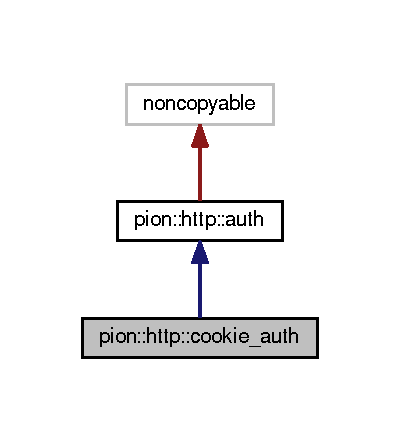
\includegraphics[width=192pt]{classpion_1_1http_1_1cookie__auth__inherit__graph}
\end{center}
\end{figure}


Collaboration diagram for pion\-:\-:http\-:\-:cookie\-\_\-auth\-:
\nopagebreak
\begin{figure}[H]
\begin{center}
\leavevmode
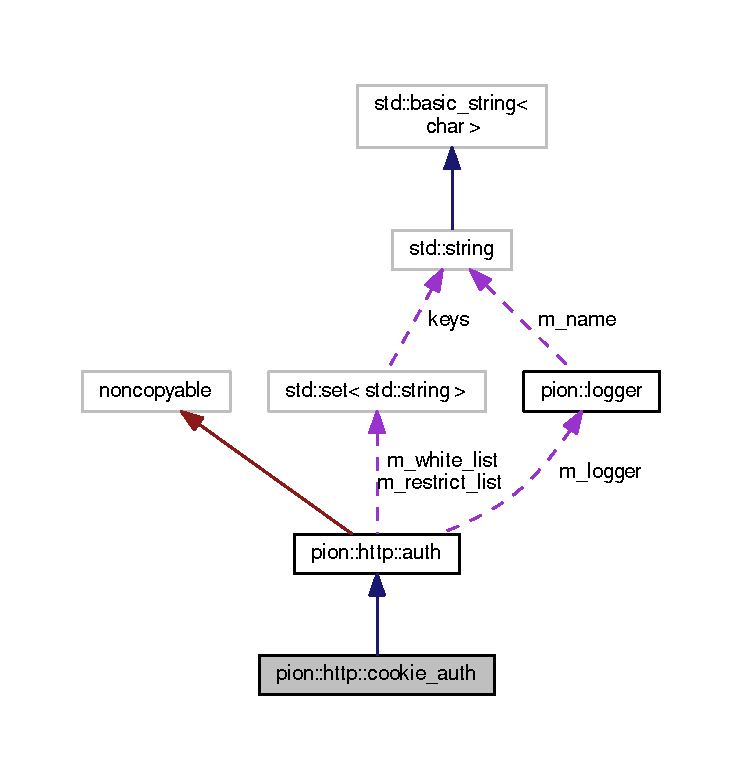
\includegraphics[width=350pt]{classpion_1_1http_1_1cookie__auth__coll__graph}
\end{center}
\end{figure}
\subsection*{Public Member Functions}
\begin{DoxyCompactItemize}
\item 
\hyperlink{classpion_1_1http_1_1cookie__auth_a769336238f9a20b74eb29be7db6e8bd3}{cookie\-\_\-auth} (\hyperlink{namespacepion_a20602680730b88b8efd08b3730d601af}{user\-\_\-manager\-\_\-ptr} user\-Manager, const std\-::string \&login=\char`\"{}/login\char`\"{}, const std\-::string \&logout=\char`\"{}/logout\char`\"{}, const std\-::string \&redirect=\char`\"{}\char`\"{})
\item 
virtual \hyperlink{classpion_1_1http_1_1cookie__auth_af161887edda25c1e95bae51a74dc843a}{$\sim$cookie\-\_\-auth} ()
\begin{DoxyCompactList}\small\item\em virtual destructor \end{DoxyCompactList}\item 
virtual bool \hyperlink{classpion_1_1http_1_1cookie__auth_a585dc707d10e0e86ba33efdfc330c83a}{handle\-\_\-request} (const \hyperlink{namespacepion_1_1http_ace432b70a9459d50ff4969a7a47f0ccb}{http\-::request\-\_\-ptr} \&http\-\_\-request\-\_\-ptr, const \hyperlink{namespacepion_1_1tcp_a6c9b7497068009f6d81d95ec0b0627d6}{tcp\-::connection\-\_\-ptr} \&tcp\-\_\-conn)
\item 
virtual void \hyperlink{classpion_1_1http_1_1cookie__auth_a87eb9ebf16f524aaf672465c37299772}{set\-\_\-option} (const std\-::string \&name, const std\-::string \&value)
\end{DoxyCompactItemize}
\subsection*{Protected Member Functions}
\begin{DoxyCompactItemize}
\item 
bool \hyperlink{classpion_1_1http_1_1cookie__auth_af6d045c98979589448f837899fd62a9e}{process\-\_\-login} (const \hyperlink{namespacepion_1_1http_ace432b70a9459d50ff4969a7a47f0ccb}{http\-::request\-\_\-ptr} \&http\-\_\-request\-\_\-ptr, const \hyperlink{namespacepion_1_1tcp_a6c9b7497068009f6d81d95ec0b0627d6}{tcp\-::connection\-\_\-ptr} \&tcp\-\_\-conn)
\item 
void \hyperlink{classpion_1_1http_1_1cookie__auth_ae0280cc2c80137330c8c85d7a085325f}{handle\-\_\-unauthorized} (const \hyperlink{namespacepion_1_1http_ace432b70a9459d50ff4969a7a47f0ccb}{http\-::request\-\_\-ptr} \&http\-\_\-request\-\_\-ptr, const \hyperlink{namespacepion_1_1tcp_a6c9b7497068009f6d81d95ec0b0627d6}{tcp\-::connection\-\_\-ptr} \&tcp\-\_\-conn)
\item 
void \hyperlink{classpion_1_1http_1_1cookie__auth_ac8bc179f19dfd34567e1bc45d1c0b7cb}{handle\-\_\-redirection} (const \hyperlink{namespacepion_1_1http_ace432b70a9459d50ff4969a7a47f0ccb}{http\-::request\-\_\-ptr} \&http\-\_\-request\-\_\-ptr, const \hyperlink{namespacepion_1_1tcp_a6c9b7497068009f6d81d95ec0b0627d6}{tcp\-::connection\-\_\-ptr} \&tcp\-\_\-conn, const std\-::string \&redirection\-\_\-url, const std\-::string \&new\-\_\-cookie=\char`\"{}\char`\"{}, bool delete\-\_\-cookie=false)
\item 
void \hyperlink{classpion_1_1http_1_1cookie__auth_a5cd041c1fa661644fb29f98d4a5f4354}{handle\-\_\-ok} (const \hyperlink{namespacepion_1_1http_ace432b70a9459d50ff4969a7a47f0ccb}{http\-::request\-\_\-ptr} \&http\-\_\-request\-\_\-ptr, const \hyperlink{namespacepion_1_1tcp_a6c9b7497068009f6d81d95ec0b0627d6}{tcp\-::connection\-\_\-ptr} \&tcp\-\_\-conn, const std\-::string \&new\-\_\-cookie=\char`\"{}\char`\"{}, bool delete\-\_\-cookie=false)
\item 
void \hyperlink{classpion_1_1http_1_1cookie__auth_a2ed6fd5500e68795955aedd6570328f4}{expire\-\_\-cache} (const boost\-::posix\-\_\-time\-::ptime \&time\-\_\-now)
\end{DoxyCompactItemize}
\subsection*{Additional Inherited Members}


\subsection{Detailed Description}
\hyperlink{classpion_1_1http_1_1cookie__auth}{cookie\-\_\-auth}\-: handles H\-T\-T\-P authentication and session management in accordance with R\-F\-C 2617 (\href{http://tools.ietf.org/html/rfc2617}{\tt http\-://tools.\-ietf.\-org/html/rfc2617} ) using cookies. 

\subsection{Constructor \& Destructor Documentation}
\hypertarget{classpion_1_1http_1_1cookie__auth_a769336238f9a20b74eb29be7db6e8bd3}{\index{pion\-::http\-::cookie\-\_\-auth@{pion\-::http\-::cookie\-\_\-auth}!cookie\-\_\-auth@{cookie\-\_\-auth}}
\index{cookie\-\_\-auth@{cookie\-\_\-auth}!pion::http::cookie_auth@{pion\-::http\-::cookie\-\_\-auth}}
\subsubsection[{cookie\-\_\-auth}]{\setlength{\rightskip}{0pt plus 5cm}pion\-::http\-::cookie\-\_\-auth\-::cookie\-\_\-auth (
\begin{DoxyParamCaption}
\item[{{\bf user\-\_\-manager\-\_\-ptr}}]{user\-Manager, }
\item[{const std\-::string \&}]{login = {\ttfamily \char`\"{}/login\char`\"{}}, }
\item[{const std\-::string \&}]{logout = {\ttfamily \char`\"{}/logout\char`\"{}}, }
\item[{const std\-::string \&}]{redirect = {\ttfamily \char`\"{}\char`\"{}}}
\end{DoxyParamCaption}
)}}\label{classpion_1_1http_1_1cookie__auth_a769336238f9a20b74eb29be7db6e8bd3}
default constructor


\begin{DoxyParams}{Parameters}
{\em user\-Manager} & \\
\hline
{\em login} & -\/ U\-R\-L resource for login request. Typical login request has format\-: \href{http://website/login?user=}{\tt http\-://website/login?user=}\char`\"{}username\char`\"{}\&pass=\char`\"{}password\char`\"{}\&url=\char`\"{}redirection\-\_\-url\char`\"{} \\
\hline
{\em logout} & -\/ U\-R\-L resource for logout request. Typical logout request has format\-: \href{http://website/logout?url=}{\tt http\-://website/logout?url=}\char`\"{}redirection\-\_\-url\char`\"{} \\
\hline
{\em redirect} & -\/ if not empty, U\-R\-L for redirection in case of authentication failure if empty -\/ send code 401 on authentication failure \\
\hline
\end{DoxyParams}


References P\-I\-O\-N\-\_\-\-G\-E\-T\-\_\-\-L\-O\-G\-G\-E\-R, and pion\-::http\-::auth\-::set\-\_\-logger().

\hypertarget{classpion_1_1http_1_1cookie__auth_af161887edda25c1e95bae51a74dc843a}{\index{pion\-::http\-::cookie\-\_\-auth@{pion\-::http\-::cookie\-\_\-auth}!$\sim$cookie\-\_\-auth@{$\sim$cookie\-\_\-auth}}
\index{$\sim$cookie\-\_\-auth@{$\sim$cookie\-\_\-auth}!pion::http::cookie_auth@{pion\-::http\-::cookie\-\_\-auth}}
\subsubsection[{$\sim$cookie\-\_\-auth}]{\setlength{\rightskip}{0pt plus 5cm}virtual pion\-::http\-::cookie\-\_\-auth\-::$\sim$cookie\-\_\-auth (
\begin{DoxyParamCaption}
{}
\end{DoxyParamCaption}
)\hspace{0.3cm}{\ttfamily [inline]}, {\ttfamily [virtual]}}}\label{classpion_1_1http_1_1cookie__auth_af161887edda25c1e95bae51a74dc843a}


virtual destructor 



\subsection{Member Function Documentation}
\hypertarget{classpion_1_1http_1_1cookie__auth_a2ed6fd5500e68795955aedd6570328f4}{\index{pion\-::http\-::cookie\-\_\-auth@{pion\-::http\-::cookie\-\_\-auth}!expire\-\_\-cache@{expire\-\_\-cache}}
\index{expire\-\_\-cache@{expire\-\_\-cache}!pion::http::cookie_auth@{pion\-::http\-::cookie\-\_\-auth}}
\subsubsection[{expire\-\_\-cache}]{\setlength{\rightskip}{0pt plus 5cm}void pion\-::http\-::cookie\-\_\-auth\-::expire\-\_\-cache (
\begin{DoxyParamCaption}
\item[{const boost\-::posix\-\_\-time\-::ptime \&}]{time\-\_\-now}
\end{DoxyParamCaption}
)\hspace{0.3cm}{\ttfamily [protected]}}}\label{classpion_1_1http_1_1cookie__auth_a2ed6fd5500e68795955aedd6570328f4}
Cache expiration cleanup. (Call it periodically) 

Referenced by handle\-\_\-request().

\hypertarget{classpion_1_1http_1_1cookie__auth_a5cd041c1fa661644fb29f98d4a5f4354}{\index{pion\-::http\-::cookie\-\_\-auth@{pion\-::http\-::cookie\-\_\-auth}!handle\-\_\-ok@{handle\-\_\-ok}}
\index{handle\-\_\-ok@{handle\-\_\-ok}!pion::http::cookie_auth@{pion\-::http\-::cookie\-\_\-auth}}
\subsubsection[{handle\-\_\-ok}]{\setlength{\rightskip}{0pt plus 5cm}void pion\-::http\-::cookie\-\_\-auth\-::handle\-\_\-ok (
\begin{DoxyParamCaption}
\item[{const {\bf http\-::request\-\_\-ptr} \&}]{http\-\_\-request\-\_\-ptr, }
\item[{const {\bf tcp\-::connection\-\_\-ptr} \&}]{tcp\-\_\-conn, }
\item[{const std\-::string \&}]{new\-\_\-cookie = {\ttfamily \char`\"{}\char`\"{}}, }
\item[{bool}]{delete\-\_\-cookie = {\ttfamily false}}
\end{DoxyParamCaption}
)\hspace{0.3cm}{\ttfamily [protected]}}}\label{classpion_1_1http_1_1cookie__auth_a5cd041c1fa661644fb29f98d4a5f4354}
used to send O\-K responses with new cookie


\begin{DoxyParams}{Parameters}
{\em http\-\_\-request\-\_\-ptr} & the new H\-T\-T\-P request to handle \\
\hline
{\em tcp\-\_\-conn} & the T\-C\-P connection that has the new request \\
\hline
\end{DoxyParams}


References pion\-::http\-::response\-\_\-writer\-::create(), pion\-::tcp\-::connection\-::finish(), pion\-::http\-::types\-::\-R\-E\-S\-P\-O\-N\-S\-E\-\_\-\-C\-O\-D\-E\-\_\-\-N\-O\-\_\-\-C\-O\-N\-T\-E\-N\-T, and pion\-::http\-::types\-::\-R\-E\-S\-P\-O\-N\-S\-E\-\_\-\-M\-E\-S\-S\-A\-G\-E\-\_\-\-N\-O\-\_\-\-C\-O\-N\-T\-E\-N\-T.



Referenced by process\-\_\-login().

\hypertarget{classpion_1_1http_1_1cookie__auth_ac8bc179f19dfd34567e1bc45d1c0b7cb}{\index{pion\-::http\-::cookie\-\_\-auth@{pion\-::http\-::cookie\-\_\-auth}!handle\-\_\-redirection@{handle\-\_\-redirection}}
\index{handle\-\_\-redirection@{handle\-\_\-redirection}!pion::http::cookie_auth@{pion\-::http\-::cookie\-\_\-auth}}
\subsubsection[{handle\-\_\-redirection}]{\setlength{\rightskip}{0pt plus 5cm}void pion\-::http\-::cookie\-\_\-auth\-::handle\-\_\-redirection (
\begin{DoxyParamCaption}
\item[{const {\bf http\-::request\-\_\-ptr} \&}]{http\-\_\-request\-\_\-ptr, }
\item[{const {\bf tcp\-::connection\-\_\-ptr} \&}]{tcp\-\_\-conn, }
\item[{const std\-::string \&}]{redirection\-\_\-url, }
\item[{const std\-::string \&}]{new\-\_\-cookie = {\ttfamily \char`\"{}\char`\"{}}, }
\item[{bool}]{delete\-\_\-cookie = {\ttfamily false}}
\end{DoxyParamCaption}
)\hspace{0.3cm}{\ttfamily [protected]}}}\label{classpion_1_1http_1_1cookie__auth_ac8bc179f19dfd34567e1bc45d1c0b7cb}
used to send redirection responses


\begin{DoxyParams}{Parameters}
{\em http\-\_\-request\-\_\-ptr} & the new H\-T\-T\-P request to handle \\
\hline
{\em tcp\-\_\-conn} & the T\-C\-P connection that has the new request \\
\hline
\end{DoxyParams}


References pion\-::http\-::response\-\_\-writer\-::create(), pion\-::tcp\-::connection\-::finish(), pion\-::http\-::types\-::\-H\-E\-A\-D\-E\-R\-\_\-\-L\-O\-C\-A\-T\-I\-O\-N, pion\-::http\-::types\-::\-R\-E\-S\-P\-O\-N\-S\-E\-\_\-\-C\-O\-D\-E\-\_\-\-F\-O\-U\-N\-D, and pion\-::http\-::types\-::\-R\-E\-S\-P\-O\-N\-S\-E\-\_\-\-M\-E\-S\-S\-A\-G\-E\-\_\-\-F\-O\-U\-N\-D.



Referenced by handle\-\_\-unauthorized(), and process\-\_\-login().

\hypertarget{classpion_1_1http_1_1cookie__auth_a585dc707d10e0e86ba33efdfc330c83a}{\index{pion\-::http\-::cookie\-\_\-auth@{pion\-::http\-::cookie\-\_\-auth}!handle\-\_\-request@{handle\-\_\-request}}
\index{handle\-\_\-request@{handle\-\_\-request}!pion::http::cookie_auth@{pion\-::http\-::cookie\-\_\-auth}}
\subsubsection[{handle\-\_\-request}]{\setlength{\rightskip}{0pt plus 5cm}bool pion\-::http\-::cookie\-\_\-auth\-::handle\-\_\-request (
\begin{DoxyParamCaption}
\item[{const {\bf http\-::request\-\_\-ptr} \&}]{http\-\_\-request\-\_\-ptr, }
\item[{const {\bf tcp\-::connection\-\_\-ptr} \&}]{tcp\-\_\-conn}
\end{DoxyParamCaption}
)\hspace{0.3cm}{\ttfamily [virtual]}}}\label{classpion_1_1http_1_1cookie__auth_a585dc707d10e0e86ba33efdfc330c83a}
attempts to validate authentication of a new H\-T\-T\-P request. If request valid, pointer to user identity object (if any) will be preserved in the request and return \char`\"{}true\char`\"{}. If request not authenticated, appropriate response is sent over tcp\-\_\-conn and return \char`\"{}false\char`\"{};

Note\-: if request matches \char`\"{}login\char`\"{} resource, then login sequences attempted. If \char`\"{}name\char`\"{} and \char`\"{}pass\char`\"{} attributes match user definition, a random cookie is created and associated with given user session. If request contains \char`\"{}url\char`\"{} attribute, then page redirection response returned. Otherwise -\/ empty 204 response.


\begin{DoxyParams}{Parameters}
{\em http\-\_\-request\-\_\-ptr} & the new H\-T\-T\-P request to handle \\
\hline
{\em tcp\-\_\-conn} & the T\-C\-P connection that has the new request\\
\hline
\end{DoxyParams}
\begin{DoxyReturn}{Returns}
true if request valid and user identity inserted into request 
\end{DoxyReturn}


Implements \hyperlink{classpion_1_1http_1_1auth_ad59da7a2c24929b7dd4d41c5679bb8bf}{pion\-::http\-::auth}.



References expire\-\_\-cache(), handle\-\_\-unauthorized(), pion\-::http\-::auth\-::need\-\_\-authentication(), and process\-\_\-login().

\hypertarget{classpion_1_1http_1_1cookie__auth_ae0280cc2c80137330c8c85d7a085325f}{\index{pion\-::http\-::cookie\-\_\-auth@{pion\-::http\-::cookie\-\_\-auth}!handle\-\_\-unauthorized@{handle\-\_\-unauthorized}}
\index{handle\-\_\-unauthorized@{handle\-\_\-unauthorized}!pion::http::cookie_auth@{pion\-::http\-::cookie\-\_\-auth}}
\subsubsection[{handle\-\_\-unauthorized}]{\setlength{\rightskip}{0pt plus 5cm}void pion\-::http\-::cookie\-\_\-auth\-::handle\-\_\-unauthorized (
\begin{DoxyParamCaption}
\item[{const {\bf http\-::request\-\_\-ptr} \&}]{http\-\_\-request\-\_\-ptr, }
\item[{const {\bf tcp\-::connection\-\_\-ptr} \&}]{tcp\-\_\-conn}
\end{DoxyParamCaption}
)\hspace{0.3cm}{\ttfamily [protected]}}}\label{classpion_1_1http_1_1cookie__auth_ae0280cc2c80137330c8c85d7a085325f}
used to send responses when access to resource is not authorized


\begin{DoxyParams}{Parameters}
{\em http\-\_\-request\-\_\-ptr} & the new H\-T\-T\-P request to handle \\
\hline
{\em tcp\-\_\-conn} & the T\-C\-P connection that has the new request \\
\hline
\end{DoxyParams}


References pion\-::http\-::response\-\_\-writer\-::create(), pion\-::tcp\-::connection\-::finish(), handle\-\_\-redirection(), pion\-::http\-::types\-::\-R\-E\-S\-P\-O\-N\-S\-E\-\_\-\-C\-O\-D\-E\-\_\-\-U\-N\-A\-U\-T\-H\-O\-R\-I\-Z\-E\-D, and pion\-::http\-::types\-::\-R\-E\-S\-P\-O\-N\-S\-E\-\_\-\-M\-E\-S\-S\-A\-G\-E\-\_\-\-U\-N\-A\-U\-T\-H\-O\-R\-I\-Z\-E\-D.



Referenced by handle\-\_\-request(), and process\-\_\-login().

\hypertarget{classpion_1_1http_1_1cookie__auth_af6d045c98979589448f837899fd62a9e}{\index{pion\-::http\-::cookie\-\_\-auth@{pion\-::http\-::cookie\-\_\-auth}!process\-\_\-login@{process\-\_\-login}}
\index{process\-\_\-login@{process\-\_\-login}!pion::http::cookie_auth@{pion\-::http\-::cookie\-\_\-auth}}
\subsubsection[{process\-\_\-login}]{\setlength{\rightskip}{0pt plus 5cm}bool pion\-::http\-::cookie\-\_\-auth\-::process\-\_\-login (
\begin{DoxyParamCaption}
\item[{const {\bf http\-::request\-\_\-ptr} \&}]{http\-\_\-request\-\_\-ptr, }
\item[{const {\bf tcp\-::connection\-\_\-ptr} \&}]{tcp\-\_\-conn}
\end{DoxyParamCaption}
)\hspace{0.3cm}{\ttfamily [protected]}}}\label{classpion_1_1http_1_1cookie__auth_af6d045c98979589448f837899fd62a9e}
check if given request is a login/logout and process it


\begin{DoxyParams}{Parameters}
{\em http\-\_\-request\-\_\-ptr} & the new H\-T\-T\-P request to handle \\
\hline
{\em tcp\-\_\-conn} & the T\-C\-P connection that has the new request\\
\hline
\end{DoxyParams}
\begin{DoxyReturn}{Returns}
true if it was a login/logout request and no future processing required. 
\end{DoxyReturn}


References pion\-::algorithm\-::base64\-\_\-encode(), handle\-\_\-ok(), handle\-\_\-redirection(), handle\-\_\-unauthorized(), pion\-::http\-::auth\-::m\-\_\-user\-\_\-manager, and pion\-::http\-::server\-::strip\-\_\-trailing\-\_\-slash().



Referenced by handle\-\_\-request().

\hypertarget{classpion_1_1http_1_1cookie__auth_a87eb9ebf16f524aaf672465c37299772}{\index{pion\-::http\-::cookie\-\_\-auth@{pion\-::http\-::cookie\-\_\-auth}!set\-\_\-option@{set\-\_\-option}}
\index{set\-\_\-option@{set\-\_\-option}!pion::http::cookie_auth@{pion\-::http\-::cookie\-\_\-auth}}
\subsubsection[{set\-\_\-option}]{\setlength{\rightskip}{0pt plus 5cm}void pion\-::http\-::cookie\-\_\-auth\-::set\-\_\-option (
\begin{DoxyParamCaption}
\item[{const std\-::string \&}]{name, }
\item[{const std\-::string \&}]{value}
\end{DoxyParamCaption}
)\hspace{0.3cm}{\ttfamily [virtual]}}}\label{classpion_1_1http_1_1cookie__auth_a87eb9ebf16f524aaf672465c37299772}
sets a configuration option Valid options\-:
\begin{DoxyItemize}
\item \char`\"{}login\char`\"{} -\/ U\-R\-L resource for login request. Typical login request has format\-: \href{http://website/login?user=}{\tt http\-://website/login?user=}\char`\"{}username\char`\"{}\&pass=\char`\"{}password\char`\"{}\&url=\char`\"{}redirection\-\_\-url\char`\"{}
\item \char`\"{}logout\char`\"{} -\/ U\-R\-L resource for logout request. Typical logout request has format\-: \href{http://website/logout?url=}{\tt http\-://website/logout?url=}\char`\"{}redirection\-\_\-url\char`\"{}
\item \char`\"{}redirect\char`\"{} -\/ if not empty, U\-R\-L for redirection in case of authentication failure if empty -\/ send code 401 on authentication failure
\end{DoxyItemize}


\begin{DoxyParams}{Parameters}
{\em name} & the name of the option to change \\
\hline
{\em value} & the value of the option \\
\hline
\end{DoxyParams}


Reimplemented from \hyperlink{classpion_1_1http_1_1auth_a49861152e006dc35880152ed0e7a6e92}{pion\-::http\-::auth}.



The documentation for this class was generated from the following files\-:\begin{DoxyCompactItemize}
\item 
include/pion/http/\hyperlink{cookie__auth_8hpp}{cookie\-\_\-auth.\-hpp}\item 
src/\hyperlink{http__cookie__auth_8cpp}{http\-\_\-cookie\-\_\-auth.\-cpp}\end{DoxyCompactItemize}

\hypertarget{structpion_1_1plugin_1_1data__type}{\section{pion\-:\-:plugin\-:\-:data\-\_\-type Struct Reference}
\label{structpion_1_1plugin_1_1data__type}\index{pion\-::plugin\-::data\-\_\-type@{pion\-::plugin\-::data\-\_\-type}}
}


{\ttfamily \#include $<$plugin.\-hpp$>$}



Collaboration diagram for pion\-:\-:plugin\-:\-:data\-\_\-type\-:
\nopagebreak
\begin{figure}[H]
\begin{center}
\leavevmode
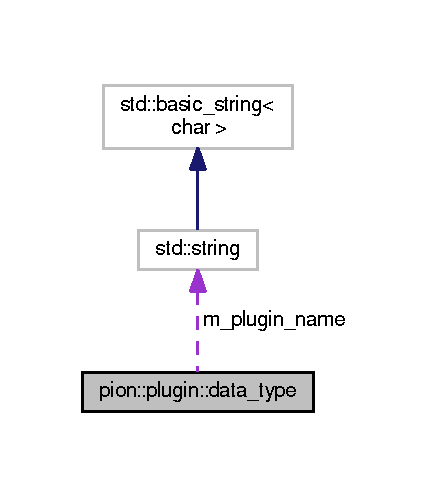
\includegraphics[width=206pt]{structpion_1_1plugin_1_1data__type__coll__graph}
\end{center}
\end{figure}
\subsection*{Public Member Functions}
\begin{DoxyCompactItemize}
\item 
\hyperlink{structpion_1_1plugin_1_1data__type_a22a8f203cafa3f97ae61fdbe607557a8}{data\-\_\-type} (void)
\begin{DoxyCompactList}\small\item\em default constructors for convenience \end{DoxyCompactList}\item 
\hyperlink{structpion_1_1plugin_1_1data__type_aece7d2d77c4c119df5859f765fa568b4}{data\-\_\-type} (const std\-::string \&plugin\-\_\-name)
\item 
\hyperlink{structpion_1_1plugin_1_1data__type_a15d9c1fdfdab4585e516b041084bbe5d}{data\-\_\-type} (const \hyperlink{structpion_1_1plugin_1_1data__type}{data\-\_\-type} \&p)
\end{DoxyCompactItemize}
\subsection*{Public Attributes}
\begin{DoxyCompactItemize}
\item 
void $\ast$ \hyperlink{structpion_1_1plugin_1_1data__type_ab53016d3d93ba84c07490a413fd01bcf}{m\-\_\-lib\-\_\-handle}
\begin{DoxyCompactList}\small\item\em symbol library loaded from a shared object file \end{DoxyCompactList}\item 
void $\ast$ \hyperlink{structpion_1_1plugin_1_1data__type_a11bd2c34a50310a4ed6042eae415c0c4}{m\-\_\-create\-\_\-func}
\begin{DoxyCompactList}\small\item\em function used to create instances of the plug-\/in object \end{DoxyCompactList}\item 
void $\ast$ \hyperlink{structpion_1_1plugin_1_1data__type_a19893ea2b05e69dfb2b346ee5f7aea41}{m\-\_\-destroy\-\_\-func}
\begin{DoxyCompactList}\small\item\em function used to destroy instances of the plug-\/in object \end{DoxyCompactList}\item 
std\-::string \hyperlink{structpion_1_1plugin_1_1data__type_a9ae35daeb06cf5f00675ff690d37db69}{m\-\_\-plugin\-\_\-name}
\begin{DoxyCompactList}\small\item\em the name of the plugin (must be unique per process) \end{DoxyCompactList}\item 
unsigned long \hyperlink{structpion_1_1plugin_1_1data__type_a2536d38120032c485b556d174ad46013}{m\-\_\-references}
\begin{DoxyCompactList}\small\item\em number of references to this class \end{DoxyCompactList}\end{DoxyCompactItemize}


\subsection{Detailed Description}
\hyperlink{structpion_1_1plugin_1_1data__type}{data\-\_\-type}\-: object to hold shared library symbols 

\subsection{Constructor \& Destructor Documentation}
\hypertarget{structpion_1_1plugin_1_1data__type_a22a8f203cafa3f97ae61fdbe607557a8}{\index{pion\-::plugin\-::data\-\_\-type@{pion\-::plugin\-::data\-\_\-type}!data\-\_\-type@{data\-\_\-type}}
\index{data\-\_\-type@{data\-\_\-type}!pion::plugin::data_type@{pion\-::plugin\-::data\-\_\-type}}
\subsubsection[{data\-\_\-type}]{\setlength{\rightskip}{0pt plus 5cm}pion\-::plugin\-::data\-\_\-type\-::data\-\_\-type (
\begin{DoxyParamCaption}
\item[{void}]{}
\end{DoxyParamCaption}
)\hspace{0.3cm}{\ttfamily [inline]}}}\label{structpion_1_1plugin_1_1data__type_a22a8f203cafa3f97ae61fdbe607557a8}


default constructors for convenience 

\hypertarget{structpion_1_1plugin_1_1data__type_aece7d2d77c4c119df5859f765fa568b4}{\index{pion\-::plugin\-::data\-\_\-type@{pion\-::plugin\-::data\-\_\-type}!data\-\_\-type@{data\-\_\-type}}
\index{data\-\_\-type@{data\-\_\-type}!pion::plugin::data_type@{pion\-::plugin\-::data\-\_\-type}}
\subsubsection[{data\-\_\-type}]{\setlength{\rightskip}{0pt plus 5cm}pion\-::plugin\-::data\-\_\-type\-::data\-\_\-type (
\begin{DoxyParamCaption}
\item[{const std\-::string \&}]{plugin\-\_\-name}
\end{DoxyParamCaption}
)\hspace{0.3cm}{\ttfamily [inline]}}}\label{structpion_1_1plugin_1_1data__type_aece7d2d77c4c119df5859f765fa568b4}
\hypertarget{structpion_1_1plugin_1_1data__type_a15d9c1fdfdab4585e516b041084bbe5d}{\index{pion\-::plugin\-::data\-\_\-type@{pion\-::plugin\-::data\-\_\-type}!data\-\_\-type@{data\-\_\-type}}
\index{data\-\_\-type@{data\-\_\-type}!pion::plugin::data_type@{pion\-::plugin\-::data\-\_\-type}}
\subsubsection[{data\-\_\-type}]{\setlength{\rightskip}{0pt plus 5cm}pion\-::plugin\-::data\-\_\-type\-::data\-\_\-type (
\begin{DoxyParamCaption}
\item[{const {\bf data\-\_\-type} \&}]{p}
\end{DoxyParamCaption}
)\hspace{0.3cm}{\ttfamily [inline]}}}\label{structpion_1_1plugin_1_1data__type_a15d9c1fdfdab4585e516b041084bbe5d}


\subsection{Member Data Documentation}
\hypertarget{structpion_1_1plugin_1_1data__type_a11bd2c34a50310a4ed6042eae415c0c4}{\index{pion\-::plugin\-::data\-\_\-type@{pion\-::plugin\-::data\-\_\-type}!m\-\_\-create\-\_\-func@{m\-\_\-create\-\_\-func}}
\index{m\-\_\-create\-\_\-func@{m\-\_\-create\-\_\-func}!pion::plugin::data_type@{pion\-::plugin\-::data\-\_\-type}}
\subsubsection[{m\-\_\-create\-\_\-func}]{\setlength{\rightskip}{0pt plus 5cm}void$\ast$ pion\-::plugin\-::data\-\_\-type\-::m\-\_\-create\-\_\-func}}\label{structpion_1_1plugin_1_1data__type_a11bd2c34a50310a4ed6042eae415c0c4}


function used to create instances of the plug-\/in object 



Referenced by pion\-::plugin\-::add\-\_\-static\-\_\-entry\-\_\-point().

\hypertarget{structpion_1_1plugin_1_1data__type_a19893ea2b05e69dfb2b346ee5f7aea41}{\index{pion\-::plugin\-::data\-\_\-type@{pion\-::plugin\-::data\-\_\-type}!m\-\_\-destroy\-\_\-func@{m\-\_\-destroy\-\_\-func}}
\index{m\-\_\-destroy\-\_\-func@{m\-\_\-destroy\-\_\-func}!pion::plugin::data_type@{pion\-::plugin\-::data\-\_\-type}}
\subsubsection[{m\-\_\-destroy\-\_\-func}]{\setlength{\rightskip}{0pt plus 5cm}void$\ast$ pion\-::plugin\-::data\-\_\-type\-::m\-\_\-destroy\-\_\-func}}\label{structpion_1_1plugin_1_1data__type_a19893ea2b05e69dfb2b346ee5f7aea41}


function used to destroy instances of the plug-\/in object 



Referenced by pion\-::plugin\-::add\-\_\-static\-\_\-entry\-\_\-point().

\hypertarget{structpion_1_1plugin_1_1data__type_ab53016d3d93ba84c07490a413fd01bcf}{\index{pion\-::plugin\-::data\-\_\-type@{pion\-::plugin\-::data\-\_\-type}!m\-\_\-lib\-\_\-handle@{m\-\_\-lib\-\_\-handle}}
\index{m\-\_\-lib\-\_\-handle@{m\-\_\-lib\-\_\-handle}!pion::plugin::data_type@{pion\-::plugin\-::data\-\_\-type}}
\subsubsection[{m\-\_\-lib\-\_\-handle}]{\setlength{\rightskip}{0pt plus 5cm}void$\ast$ pion\-::plugin\-::data\-\_\-type\-::m\-\_\-lib\-\_\-handle}}\label{structpion_1_1plugin_1_1data__type_ab53016d3d93ba84c07490a413fd01bcf}


symbol library loaded from a shared object file 



Referenced by pion\-::plugin\-::add\-\_\-static\-\_\-entry\-\_\-point(), pion\-::plugin\-::get\-\_\-all\-\_\-plugin\-\_\-names(), and pion\-::plugin\-::release\-\_\-data().

\hypertarget{structpion_1_1plugin_1_1data__type_a9ae35daeb06cf5f00675ff690d37db69}{\index{pion\-::plugin\-::data\-\_\-type@{pion\-::plugin\-::data\-\_\-type}!m\-\_\-plugin\-\_\-name@{m\-\_\-plugin\-\_\-name}}
\index{m\-\_\-plugin\-\_\-name@{m\-\_\-plugin\-\_\-name}!pion::plugin::data_type@{pion\-::plugin\-::data\-\_\-type}}
\subsubsection[{m\-\_\-plugin\-\_\-name}]{\setlength{\rightskip}{0pt plus 5cm}std\-::string pion\-::plugin\-::data\-\_\-type\-::m\-\_\-plugin\-\_\-name}}\label{structpion_1_1plugin_1_1data__type_a9ae35daeb06cf5f00675ff690d37db69}


the name of the plugin (must be unique per process) 



Referenced by pion\-::plugin\-::get\-\_\-all\-\_\-plugin\-\_\-names(), pion\-::plugin\-::open\-\_\-file(), and pion\-::plugin\-::release\-\_\-data().

\hypertarget{structpion_1_1plugin_1_1data__type_a2536d38120032c485b556d174ad46013}{\index{pion\-::plugin\-::data\-\_\-type@{pion\-::plugin\-::data\-\_\-type}!m\-\_\-references@{m\-\_\-references}}
\index{m\-\_\-references@{m\-\_\-references}!pion::plugin::data_type@{pion\-::plugin\-::data\-\_\-type}}
\subsubsection[{m\-\_\-references}]{\setlength{\rightskip}{0pt plus 5cm}unsigned long pion\-::plugin\-::data\-\_\-type\-::m\-\_\-references}}\label{structpion_1_1plugin_1_1data__type_a2536d38120032c485b556d174ad46013}


number of references to this class 



Referenced by pion\-::plugin\-::grab\-\_\-data(), pion\-::plugin\-::open(), pion\-::plugin\-::open\-\_\-file(), and pion\-::plugin\-::release\-\_\-data().



The documentation for this struct was generated from the following file\-:\begin{DoxyCompactItemize}
\item 
include/pion/\hyperlink{plugin_8hpp}{plugin.\-hpp}\end{DoxyCompactItemize}

\hypertarget{classpion_1_1spdy_1_1decompressor}{\section{pion\-:\-:spdy\-:\-:decompressor Class Reference}
\label{classpion_1_1spdy_1_1decompressor}\index{pion\-::spdy\-::decompressor@{pion\-::spdy\-::decompressor}}
}


{\ttfamily \#include $<$decompressor.\-hpp$>$}

\subsection*{Public Types}
\begin{DoxyCompactItemize}
\item 
enum \hyperlink{classpion_1_1spdy_1_1decompressor_a9fb34f033b4d95e5f23fa9b0d03c4818}{data\-\_\-size\-\_\-t} \{ \hyperlink{classpion_1_1spdy_1_1decompressor_a9fb34f033b4d95e5f23fa9b0d03c4818a44ab53316cb7bd9c9d66621b6e537e08}{M\-A\-X\-\_\-\-U\-N\-C\-O\-M\-P\-R\-E\-S\-S\-E\-D\-\_\-\-D\-A\-T\-A\-\_\-\-B\-U\-F\-\_\-\-S\-I\-Z\-E} = 16384
 \}
\begin{DoxyCompactList}\small\item\em data size constants \end{DoxyCompactList}\end{DoxyCompactItemize}
\subsection*{Public Member Functions}
\begin{DoxyCompactItemize}
\item 
\hyperlink{classpion_1_1spdy_1_1decompressor_ab60b284101b5b7ffedc2fb4daab2f77d}{decompressor} ()
\begin{DoxyCompactList}\small\item\em constructs a new decompressor object (default constructor) \end{DoxyCompactList}\item 
\hyperlink{classpion_1_1spdy_1_1decompressor_adc518d8ec91bb78d58077f7fb661881f}{$\sim$decompressor} ()
\begin{DoxyCompactList}\small\item\em destructor \end{DoxyCompactList}\item 
char $\ast$ \hyperlink{classpion_1_1spdy_1_1decompressor_a9e6e8b557657365b9e30a501c9bdd00b}{decompress} (const char $\ast$compressed\-\_\-data\-\_\-ptr, boost\-::uint32\-\_\-t stream\-\_\-id, const \hyperlink{structpion_1_1spdy_1_1spdy__control__frame__info}{spdy\-\_\-control\-\_\-frame\-\_\-info} \&frame, boost\-::uint32\-\_\-t header\-\_\-block\-\_\-length)
\end{DoxyCompactItemize}
\subsection*{Protected Member Functions}
\begin{DoxyCompactItemize}
\item 
bool \hyperlink{classpion_1_1spdy_1_1decompressor_ab6c148eb985c1e016235cef3863913c8}{spdy\-\_\-decompress\-\_\-header} (const char $\ast$compressed\-\_\-data\-\_\-ptr, z\-\_\-streamp decomp, boost\-::uint32\-\_\-t length, boost\-::uint32\-\_\-t \&uncomp\-\_\-length)
\end{DoxyCompactItemize}


\subsection{Detailed Description}
S\-P\-D\-Y\-Decompressor \-: Decompresses S\-P\-D\-Y frames 

\subsection{Member Enumeration Documentation}
\hypertarget{classpion_1_1spdy_1_1decompressor_a9fb34f033b4d95e5f23fa9b0d03c4818}{\index{pion\-::spdy\-::decompressor@{pion\-::spdy\-::decompressor}!data\-\_\-size\-\_\-t@{data\-\_\-size\-\_\-t}}
\index{data\-\_\-size\-\_\-t@{data\-\_\-size\-\_\-t}!pion::spdy::decompressor@{pion\-::spdy\-::decompressor}}
\subsubsection[{data\-\_\-size\-\_\-t}]{\setlength{\rightskip}{0pt plus 5cm}enum {\bf pion\-::spdy\-::decompressor\-::data\-\_\-size\-\_\-t}}}\label{classpion_1_1spdy_1_1decompressor_a9fb34f033b4d95e5f23fa9b0d03c4818}


data size constants 

\begin{Desc}
\item[Enumerator]\par
\begin{description}
\index{M\-A\-X\-\_\-\-U\-N\-C\-O\-M\-P\-R\-E\-S\-S\-E\-D\-\_\-\-D\-A\-T\-A\-\_\-\-B\-U\-F\-\_\-\-S\-I\-Z\-E@{M\-A\-X\-\_\-\-U\-N\-C\-O\-M\-P\-R\-E\-S\-S\-E\-D\-\_\-\-D\-A\-T\-A\-\_\-\-B\-U\-F\-\_\-\-S\-I\-Z\-E}!pion\-::spdy\-::decompressor@{pion\-::spdy\-::decompressor}}\index{pion\-::spdy\-::decompressor@{pion\-::spdy\-::decompressor}!M\-A\-X\-\_\-\-U\-N\-C\-O\-M\-P\-R\-E\-S\-S\-E\-D\-\_\-\-D\-A\-T\-A\-\_\-\-B\-U\-F\-\_\-\-S\-I\-Z\-E@{M\-A\-X\-\_\-\-U\-N\-C\-O\-M\-P\-R\-E\-S\-S\-E\-D\-\_\-\-D\-A\-T\-A\-\_\-\-B\-U\-F\-\_\-\-S\-I\-Z\-E}}\item[{\em 
\hypertarget{classpion_1_1spdy_1_1decompressor_a9fb34f033b4d95e5f23fa9b0d03c4818a44ab53316cb7bd9c9d66621b6e537e08}{M\-A\-X\-\_\-\-U\-N\-C\-O\-M\-P\-R\-E\-S\-S\-E\-D\-\_\-\-D\-A\-T\-A\-\_\-\-B\-U\-F\-\_\-\-S\-I\-Z\-E}\label{classpion_1_1spdy_1_1decompressor_a9fb34f033b4d95e5f23fa9b0d03c4818a44ab53316cb7bd9c9d66621b6e537e08}
}]maximum size of an uncompressed spdy header \end{description}
\end{Desc}


\subsection{Constructor \& Destructor Documentation}
\hypertarget{classpion_1_1spdy_1_1decompressor_ab60b284101b5b7ffedc2fb4daab2f77d}{\index{pion\-::spdy\-::decompressor@{pion\-::spdy\-::decompressor}!decompressor@{decompressor}}
\index{decompressor@{decompressor}!pion::spdy::decompressor@{pion\-::spdy\-::decompressor}}
\subsubsection[{decompressor}]{\setlength{\rightskip}{0pt plus 5cm}pion\-::spdy\-::decompressor\-::decompressor (
\begin{DoxyParamCaption}
{}
\end{DoxyParamCaption}
)}}\label{classpion_1_1spdy_1_1decompressor_ab60b284101b5b7ffedc2fb4daab2f77d}


constructs a new decompressor object (default constructor) 

\hypertarget{classpion_1_1spdy_1_1decompressor_adc518d8ec91bb78d58077f7fb661881f}{\index{pion\-::spdy\-::decompressor@{pion\-::spdy\-::decompressor}!$\sim$decompressor@{$\sim$decompressor}}
\index{$\sim$decompressor@{$\sim$decompressor}!pion::spdy::decompressor@{pion\-::spdy\-::decompressor}}
\subsubsection[{$\sim$decompressor}]{\setlength{\rightskip}{0pt plus 5cm}pion\-::spdy\-::decompressor\-::$\sim$decompressor (
\begin{DoxyParamCaption}
{}
\end{DoxyParamCaption}
)}}\label{classpion_1_1spdy_1_1decompressor_adc518d8ec91bb78d58077f7fb661881f}


destructor 



\subsection{Member Function Documentation}
\hypertarget{classpion_1_1spdy_1_1decompressor_a9e6e8b557657365b9e30a501c9bdd00b}{\index{pion\-::spdy\-::decompressor@{pion\-::spdy\-::decompressor}!decompress@{decompress}}
\index{decompress@{decompress}!pion::spdy::decompressor@{pion\-::spdy\-::decompressor}}
\subsubsection[{decompress}]{\setlength{\rightskip}{0pt plus 5cm}char $\ast$ pion\-::spdy\-::decompressor\-::decompress (
\begin{DoxyParamCaption}
\item[{const char $\ast$}]{compressed\-\_\-data\-\_\-ptr, }
\item[{boost\-::uint32\-\_\-t}]{stream\-\_\-id, }
\item[{const {\bf spdy\-\_\-control\-\_\-frame\-\_\-info} \&}]{frame, }
\item[{boost\-::uint32\-\_\-t}]{header\-\_\-block\-\_\-length}
\end{DoxyParamCaption}
)}}\label{classpion_1_1spdy_1_1decompressor_a9e6e8b557657365b9e30a501c9bdd00b}
decompresses the http content

\begin{DoxyReturn}{Returns}
the uncompressed string, or null on failure 
\end{DoxyReturn}
Get our decompressor. 

References spdy\-\_\-decompress\-\_\-header(), S\-P\-D\-Y\-\_\-\-H\-E\-A\-D\-E\-R\-S, S\-P\-D\-Y\-\_\-\-S\-Y\-N\-\_\-\-R\-E\-P\-L\-Y, S\-P\-D\-Y\-\_\-\-S\-Y\-N\-\_\-\-S\-T\-R\-E\-A\-M, and pion\-::spdy\-::spdy\-\_\-control\-\_\-frame\-\_\-info\-::type.

\hypertarget{classpion_1_1spdy_1_1decompressor_ab6c148eb985c1e016235cef3863913c8}{\index{pion\-::spdy\-::decompressor@{pion\-::spdy\-::decompressor}!spdy\-\_\-decompress\-\_\-header@{spdy\-\_\-decompress\-\_\-header}}
\index{spdy\-\_\-decompress\-\_\-header@{spdy\-\_\-decompress\-\_\-header}!pion::spdy::decompressor@{pion\-::spdy\-::decompressor}}
\subsubsection[{spdy\-\_\-decompress\-\_\-header}]{\setlength{\rightskip}{0pt plus 5cm}bool pion\-::spdy\-::decompressor\-::spdy\-\_\-decompress\-\_\-header (
\begin{DoxyParamCaption}
\item[{const char $\ast$}]{compressed\-\_\-data\-\_\-ptr, }
\item[{z\-\_\-streamp}]{decomp, }
\item[{boost\-::uint32\-\_\-t}]{length, }
\item[{boost\-::uint32\-\_\-t \&}]{uncomp\-\_\-length}
\end{DoxyParamCaption}
)\hspace{0.3cm}{\ttfamily [protected]}}}\label{classpion_1_1spdy_1_1decompressor_ab6c148eb985c1e016235cef3863913c8}
decompresses the spdy header

\begin{DoxyReturn}{Returns}
true if successful 
\end{DoxyReturn}


References M\-A\-X\-\_\-\-U\-N\-C\-O\-M\-P\-R\-E\-S\-S\-E\-D\-\_\-\-D\-A\-T\-A\-\_\-\-B\-U\-F\-\_\-\-S\-I\-Z\-E.



Referenced by decompress().



The documentation for this class was generated from the following files\-:\begin{DoxyCompactItemize}
\item 
include/pion/spdy/\hyperlink{decompressor_8hpp}{decompressor.\-hpp}\item 
src/\hyperlink{spdy__decompressor_8cpp}{spdy\-\_\-decompressor.\-cpp}\end{DoxyCompactItemize}

\hypertarget{classpion_1_1error_1_1directory__not__found}{\section{pion\-:\-:error\-:\-:directory\-\_\-not\-\_\-found Class Reference}
\label{classpion_1_1error_1_1directory__not__found}\index{pion\-::error\-::directory\-\_\-not\-\_\-found@{pion\-::error\-::directory\-\_\-not\-\_\-found}}
}


exception thrown if a required directory is not found  




{\ttfamily \#include $<$error.\-hpp$>$}



Inheritance diagram for pion\-:\-:error\-:\-:directory\-\_\-not\-\_\-found\-:
\nopagebreak
\begin{figure}[H]
\begin{center}
\leavevmode
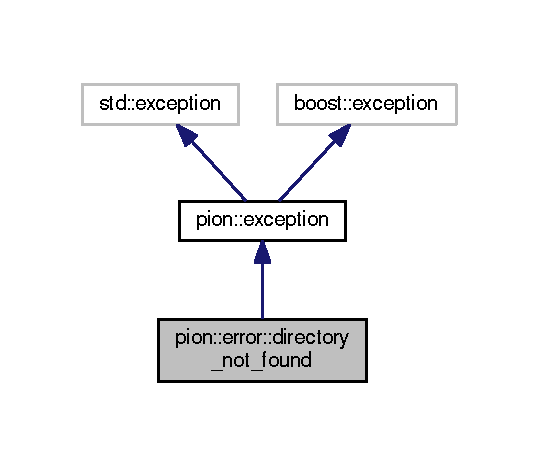
\includegraphics[width=259pt]{classpion_1_1error_1_1directory__not__found__inherit__graph}
\end{center}
\end{figure}


Collaboration diagram for pion\-:\-:error\-:\-:directory\-\_\-not\-\_\-found\-:
\nopagebreak
\begin{figure}[H]
\begin{center}
\leavevmode
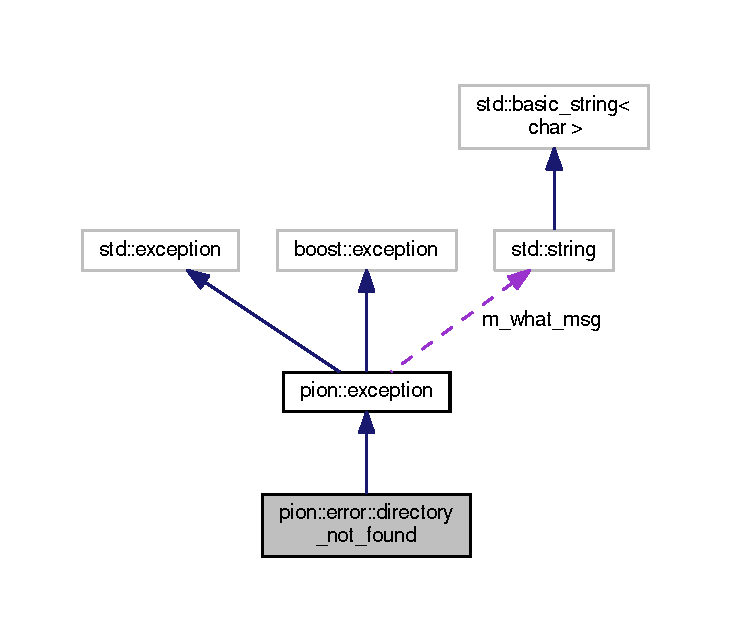
\includegraphics[width=350pt]{classpion_1_1error_1_1directory__not__found__coll__graph}
\end{center}
\end{figure}
\subsection*{Additional Inherited Members}


\subsection{Detailed Description}
exception thrown if a required directory is not found 

The documentation for this class was generated from the following file\-:\begin{DoxyCompactItemize}
\item 
include/pion/\hyperlink{error_8hpp}{error.\-hpp}\end{DoxyCompactItemize}

\hypertarget{classpion_1_1error_1_1duplicate__plugin}{\section{pion\-:\-:error\-:\-:duplicate\-\_\-plugin Class Reference}
\label{classpion_1_1error_1_1duplicate__plugin}\index{pion\-::error\-::duplicate\-\_\-plugin@{pion\-::error\-::duplicate\-\_\-plugin}}
}


exception thrown if we try to add or load a duplicate plugin  




{\ttfamily \#include $<$error.\-hpp$>$}



Inheritance diagram for pion\-:\-:error\-:\-:duplicate\-\_\-plugin\-:
\nopagebreak
\begin{figure}[H]
\begin{center}
\leavevmode
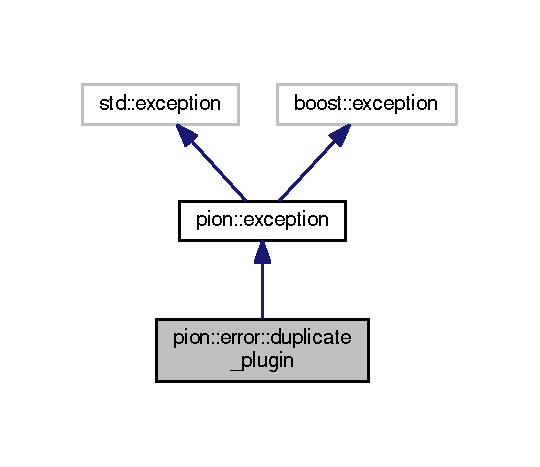
\includegraphics[width=259pt]{classpion_1_1error_1_1duplicate__plugin__inherit__graph}
\end{center}
\end{figure}


Collaboration diagram for pion\-:\-:error\-:\-:duplicate\-\_\-plugin\-:
\nopagebreak
\begin{figure}[H]
\begin{center}
\leavevmode
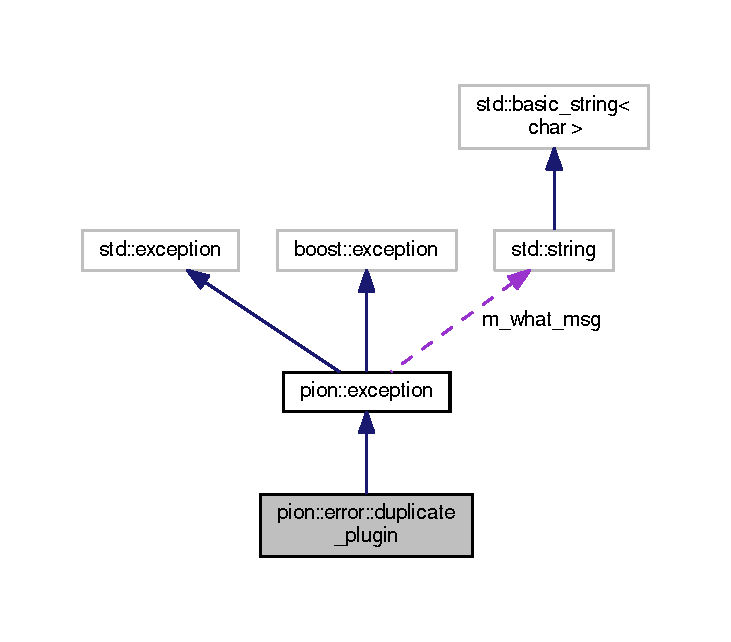
\includegraphics[width=350pt]{classpion_1_1error_1_1duplicate__plugin__coll__graph}
\end{center}
\end{figure}
\subsection*{Additional Inherited Members}


\subsection{Detailed Description}
exception thrown if we try to add or load a duplicate plugin 

The documentation for this class was generated from the following file\-:\begin{DoxyCompactItemize}
\item 
include/pion/\hyperlink{error_8hpp}{error.\-hpp}\end{DoxyCompactItemize}

\hypertarget{classpion_1_1http_1_1parser_1_1error__category__t}{\section{pion\-:\-:http\-:\-:parser\-:\-:error\-\_\-category\-\_\-t Class Reference}
\label{classpion_1_1http_1_1parser_1_1error__category__t}\index{pion\-::http\-::parser\-::error\-\_\-category\-\_\-t@{pion\-::http\-::parser\-::error\-\_\-category\-\_\-t}}
}


class-\/specific error category  




{\ttfamily \#include $<$parser.\-hpp$>$}



Inheritance diagram for pion\-:\-:http\-:\-:parser\-:\-:error\-\_\-category\-\_\-t\-:
\nopagebreak
\begin{figure}[H]
\begin{center}
\leavevmode
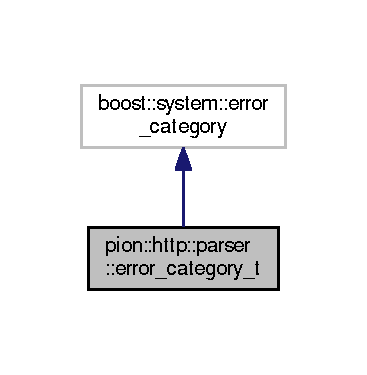
\includegraphics[width=176pt]{classpion_1_1http_1_1parser_1_1error__category__t__inherit__graph}
\end{center}
\end{figure}


Collaboration diagram for pion\-:\-:http\-:\-:parser\-:\-:error\-\_\-category\-\_\-t\-:
\nopagebreak
\begin{figure}[H]
\begin{center}
\leavevmode
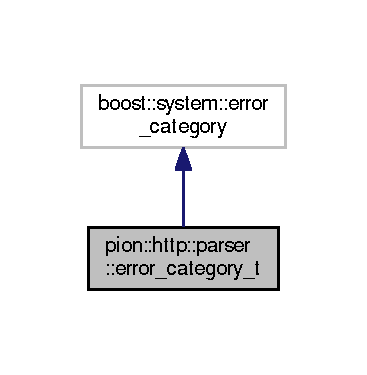
\includegraphics[width=176pt]{classpion_1_1http_1_1parser_1_1error__category__t__coll__graph}
\end{center}
\end{figure}
\subsection*{Public Member Functions}
\begin{DoxyCompactItemize}
\item 
const char $\ast$ \hyperlink{classpion_1_1http_1_1parser_1_1error__category__t_a8b321a84e109e48fc9313115b27359cf}{name} () const \hyperlink{spdy_2parser_8hpp_a66e2f4d9ec8a0ac5a2dddbfa9a88fb5b}{B\-O\-O\-S\-T\-\_\-\-S\-Y\-S\-T\-E\-M\-\_\-\-N\-O\-E\-X\-C\-E\-P\-T}
\item 
std\-::string \hyperlink{classpion_1_1http_1_1parser_1_1error__category__t_aeb4d9dcd75fe161241e0f691cfab99d9}{message} (int ev) const 
\end{DoxyCompactItemize}


\subsection{Detailed Description}
class-\/specific error category 

\subsection{Member Function Documentation}
\hypertarget{classpion_1_1http_1_1parser_1_1error__category__t_aeb4d9dcd75fe161241e0f691cfab99d9}{\index{pion\-::http\-::parser\-::error\-\_\-category\-\_\-t@{pion\-::http\-::parser\-::error\-\_\-category\-\_\-t}!message@{message}}
\index{message@{message}!pion::http::parser::error_category_t@{pion\-::http\-::parser\-::error\-\_\-category\-\_\-t}}
\subsubsection[{message}]{\setlength{\rightskip}{0pt plus 5cm}std\-::string pion\-::http\-::parser\-::error\-\_\-category\-\_\-t\-::message (
\begin{DoxyParamCaption}
\item[{int}]{ev}
\end{DoxyParamCaption}
) const\hspace{0.3cm}{\ttfamily [inline]}}}\label{classpion_1_1http_1_1parser_1_1error__category__t_aeb4d9dcd75fe161241e0f691cfab99d9}
\hypertarget{classpion_1_1http_1_1parser_1_1error__category__t_a8b321a84e109e48fc9313115b27359cf}{\index{pion\-::http\-::parser\-::error\-\_\-category\-\_\-t@{pion\-::http\-::parser\-::error\-\_\-category\-\_\-t}!name@{name}}
\index{name@{name}!pion::http::parser::error_category_t@{pion\-::http\-::parser\-::error\-\_\-category\-\_\-t}}
\subsubsection[{name}]{\setlength{\rightskip}{0pt plus 5cm}const char$\ast$ pion\-::http\-::parser\-::error\-\_\-category\-\_\-t\-::name (
\begin{DoxyParamCaption}
{}
\end{DoxyParamCaption}
) const\hspace{0.3cm}{\ttfamily [inline]}}}\label{classpion_1_1http_1_1parser_1_1error__category__t_a8b321a84e109e48fc9313115b27359cf}


The documentation for this class was generated from the following file\-:\begin{DoxyCompactItemize}
\item 
include/pion/http/\hyperlink{http_2parser_8hpp}{parser.\-hpp}\end{DoxyCompactItemize}

\hypertarget{classpion_1_1spdy_1_1parser_1_1error__category__t}{\section{pion\-:\-:spdy\-:\-:parser\-:\-:error\-\_\-category\-\_\-t Class Reference}
\label{classpion_1_1spdy_1_1parser_1_1error__category__t}\index{pion\-::spdy\-::parser\-::error\-\_\-category\-\_\-t@{pion\-::spdy\-::parser\-::error\-\_\-category\-\_\-t}}
}


class-\/specific error category  




{\ttfamily \#include $<$parser.\-hpp$>$}



Inheritance diagram for pion\-:\-:spdy\-:\-:parser\-:\-:error\-\_\-category\-\_\-t\-:
\nopagebreak
\begin{figure}[H]
\begin{center}
\leavevmode
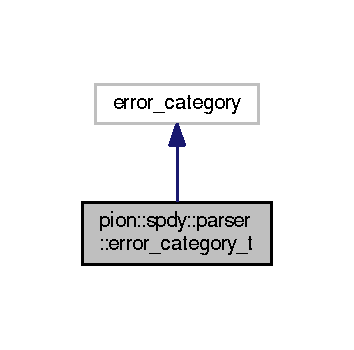
\includegraphics[width=170pt]{classpion_1_1spdy_1_1parser_1_1error__category__t__inherit__graph}
\end{center}
\end{figure}


Collaboration diagram for pion\-:\-:spdy\-:\-:parser\-:\-:error\-\_\-category\-\_\-t\-:
\nopagebreak
\begin{figure}[H]
\begin{center}
\leavevmode
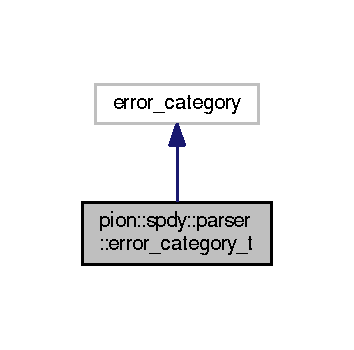
\includegraphics[width=170pt]{classpion_1_1spdy_1_1parser_1_1error__category__t__coll__graph}
\end{center}
\end{figure}
\subsection*{Public Member Functions}
\begin{DoxyCompactItemize}
\item 
const char $\ast$ \hyperlink{classpion_1_1spdy_1_1parser_1_1error__category__t_a6ef5ae1be50c4354025c754c28bee948}{name} () const \hyperlink{spdy_2parser_8hpp_a66e2f4d9ec8a0ac5a2dddbfa9a88fb5b}{B\-O\-O\-S\-T\-\_\-\-S\-Y\-S\-T\-E\-M\-\_\-\-N\-O\-E\-X\-C\-E\-P\-T}
\item 
std\-::string \hyperlink{classpion_1_1spdy_1_1parser_1_1error__category__t_a89956154b900ad8cfa578041c11c20de}{message} (int ev) const 
\end{DoxyCompactItemize}


\subsection{Detailed Description}
class-\/specific error category 

\subsection{Member Function Documentation}
\hypertarget{classpion_1_1spdy_1_1parser_1_1error__category__t_a89956154b900ad8cfa578041c11c20de}{\index{pion\-::spdy\-::parser\-::error\-\_\-category\-\_\-t@{pion\-::spdy\-::parser\-::error\-\_\-category\-\_\-t}!message@{message}}
\index{message@{message}!pion::spdy::parser::error_category_t@{pion\-::spdy\-::parser\-::error\-\_\-category\-\_\-t}}
\subsubsection[{message}]{\setlength{\rightskip}{0pt plus 5cm}std\-::string pion\-::spdy\-::parser\-::error\-\_\-category\-\_\-t\-::message (
\begin{DoxyParamCaption}
\item[{int}]{ev}
\end{DoxyParamCaption}
) const\hspace{0.3cm}{\ttfamily [inline]}}}\label{classpion_1_1spdy_1_1parser_1_1error__category__t_a89956154b900ad8cfa578041c11c20de}
\hypertarget{classpion_1_1spdy_1_1parser_1_1error__category__t_a6ef5ae1be50c4354025c754c28bee948}{\index{pion\-::spdy\-::parser\-::error\-\_\-category\-\_\-t@{pion\-::spdy\-::parser\-::error\-\_\-category\-\_\-t}!name@{name}}
\index{name@{name}!pion::spdy::parser::error_category_t@{pion\-::spdy\-::parser\-::error\-\_\-category\-\_\-t}}
\subsubsection[{name}]{\setlength{\rightskip}{0pt plus 5cm}const char$\ast$ pion\-::spdy\-::parser\-::error\-\_\-category\-\_\-t\-::name (
\begin{DoxyParamCaption}
{}
\end{DoxyParamCaption}
) const\hspace{0.3cm}{\ttfamily [inline]}}}\label{classpion_1_1spdy_1_1parser_1_1error__category__t_a6ef5ae1be50c4354025c754c28bee948}


The documentation for this class was generated from the following file\-:\begin{DoxyCompactItemize}
\item 
include/pion/spdy/\hyperlink{spdy_2parser_8hpp}{parser.\-hpp}\end{DoxyCompactItemize}

\hypertarget{classpion_1_1exception}{\section{pion\-:\-:exception Class Reference}
\label{classpion_1_1exception}\index{pion\-::exception@{pion\-::exception}}
}


{\ttfamily \#include $<$error.\-hpp$>$}



Inheritance diagram for pion\-:\-:exception\-:
\nopagebreak
\begin{figure}[H]
\begin{center}
\leavevmode
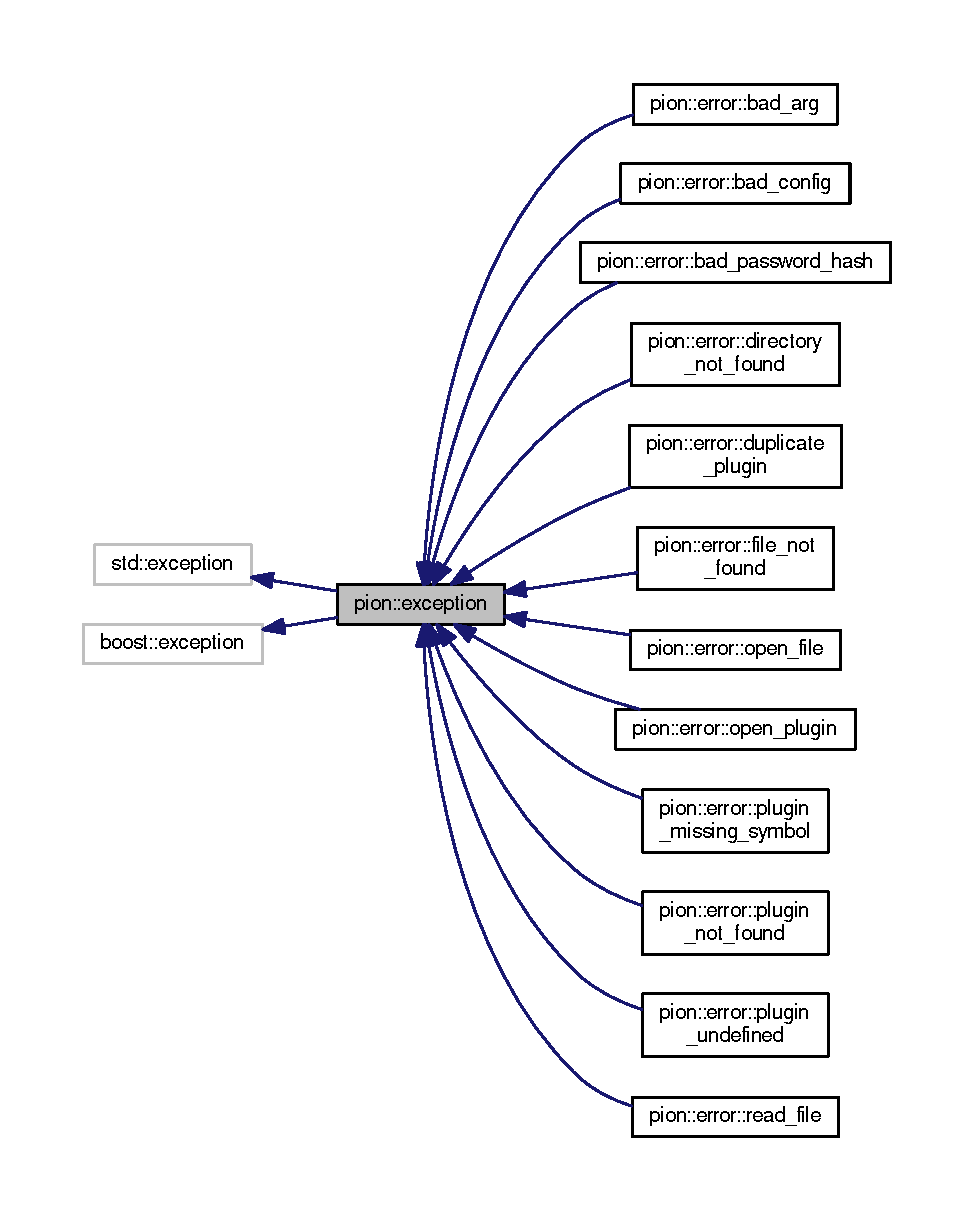
\includegraphics[width=350pt]{classpion_1_1exception__inherit__graph}
\end{center}
\end{figure}


Collaboration diagram for pion\-:\-:exception\-:
\nopagebreak
\begin{figure}[H]
\begin{center}
\leavevmode
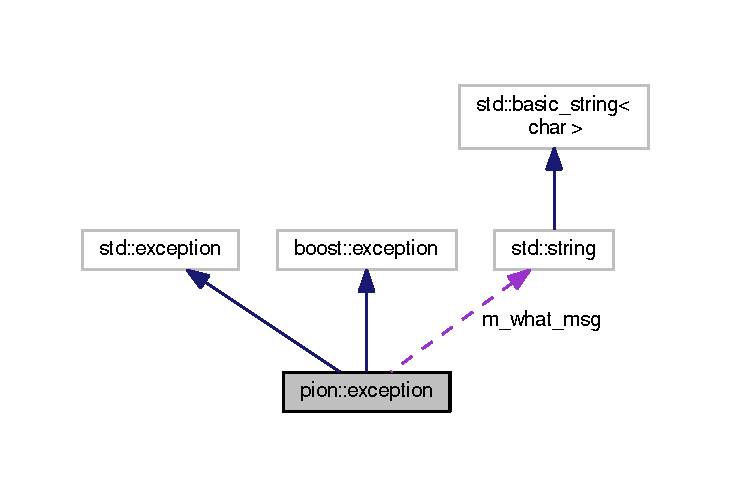
\includegraphics[width=350pt]{classpion_1_1exception__coll__graph}
\end{center}
\end{figure}
\subsection*{Public Member Functions}
\begin{DoxyCompactItemize}
\item 
\hyperlink{classpion_1_1exception_a031f13a415ee022db9f14fea59eb5c74}{exception} ()
\item 
\hyperlink{classpion_1_1exception_aaec2c298dcad795cf4b66c18c440dfcb}{exception} (const std\-::string \&msg)
\item 
\hyperlink{classpion_1_1exception_a970d4da1afade252a5024dec90aa48d7}{exception} (const char $\ast$const msg)
\item 
virtual \hyperlink{classpion_1_1exception_aebcf314a4a7e4e7636ee25eb4a393d5c}{$\sim$exception} ()  throw ()
\item 
virtual const char $\ast$ \hyperlink{classpion_1_1exception_a40a62768258b7772de35398177dbd6ce}{what} () const   throw ()
\end{DoxyCompactItemize}
\subsection*{Protected Member Functions}
\begin{DoxyCompactItemize}
\item 
void \hyperlink{classpion_1_1exception_ab7aa00d924b61114cd98a96ec8a78a98}{set\-\_\-what\-\_\-msg} (const char $\ast$const msg=N\-U\-L\-L, const std\-::string $\ast$const arg1=N\-U\-L\-L, const std\-::string $\ast$const arg2=N\-U\-L\-L, const std\-::string $\ast$const arg3=N\-U\-L\-L) const 
\item 
virtual void \hyperlink{classpion_1_1exception_a13a7f06c1c25bfa139447f5ac091f85f}{update\-\_\-what\-\_\-msg} () const 
\end{DoxyCompactItemize}
\subsection*{Protected Attributes}
\begin{DoxyCompactItemize}
\item 
std\-::string \hyperlink{classpion_1_1exception_ae1c8e87bb8013e9abccc5326bdcbab72}{m\-\_\-what\-\_\-msg}
\end{DoxyCompactItemize}


\subsection{Constructor \& Destructor Documentation}
\hypertarget{classpion_1_1exception_a031f13a415ee022db9f14fea59eb5c74}{\index{pion\-::exception@{pion\-::exception}!exception@{exception}}
\index{exception@{exception}!pion::exception@{pion\-::exception}}
\subsubsection[{exception}]{\setlength{\rightskip}{0pt plus 5cm}pion\-::exception\-::exception (
\begin{DoxyParamCaption}
{}
\end{DoxyParamCaption}
)\hspace{0.3cm}{\ttfamily [inline]}}}\label{classpion_1_1exception_a031f13a415ee022db9f14fea59eb5c74}
\hypertarget{classpion_1_1exception_aaec2c298dcad795cf4b66c18c440dfcb}{\index{pion\-::exception@{pion\-::exception}!exception@{exception}}
\index{exception@{exception}!pion::exception@{pion\-::exception}}
\subsubsection[{exception}]{\setlength{\rightskip}{0pt plus 5cm}pion\-::exception\-::exception (
\begin{DoxyParamCaption}
\item[{const std\-::string \&}]{msg}
\end{DoxyParamCaption}
)\hspace{0.3cm}{\ttfamily [inline]}}}\label{classpion_1_1exception_aaec2c298dcad795cf4b66c18c440dfcb}
\hypertarget{classpion_1_1exception_a970d4da1afade252a5024dec90aa48d7}{\index{pion\-::exception@{pion\-::exception}!exception@{exception}}
\index{exception@{exception}!pion::exception@{pion\-::exception}}
\subsubsection[{exception}]{\setlength{\rightskip}{0pt plus 5cm}pion\-::exception\-::exception (
\begin{DoxyParamCaption}
\item[{const char $\ast$const}]{msg}
\end{DoxyParamCaption}
)\hspace{0.3cm}{\ttfamily [inline]}}}\label{classpion_1_1exception_a970d4da1afade252a5024dec90aa48d7}
\hypertarget{classpion_1_1exception_aebcf314a4a7e4e7636ee25eb4a393d5c}{\index{pion\-::exception@{pion\-::exception}!$\sim$exception@{$\sim$exception}}
\index{$\sim$exception@{$\sim$exception}!pion::exception@{pion\-::exception}}
\subsubsection[{$\sim$exception}]{\setlength{\rightskip}{0pt plus 5cm}virtual pion\-::exception\-::$\sim$exception (
\begin{DoxyParamCaption}
{}
\end{DoxyParamCaption}
) throw  ) \hspace{0.3cm}{\ttfamily [inline]}, {\ttfamily [virtual]}}}\label{classpion_1_1exception_aebcf314a4a7e4e7636ee25eb4a393d5c}


\subsection{Member Function Documentation}
\hypertarget{classpion_1_1exception_ab7aa00d924b61114cd98a96ec8a78a98}{\index{pion\-::exception@{pion\-::exception}!set\-\_\-what\-\_\-msg@{set\-\_\-what\-\_\-msg}}
\index{set\-\_\-what\-\_\-msg@{set\-\_\-what\-\_\-msg}!pion::exception@{pion\-::exception}}
\subsubsection[{set\-\_\-what\-\_\-msg}]{\setlength{\rightskip}{0pt plus 5cm}void pion\-::exception\-::set\-\_\-what\-\_\-msg (
\begin{DoxyParamCaption}
\item[{const char $\ast$const}]{msg = {\ttfamily NULL}, }
\item[{const std\-::string $\ast$const}]{arg1 = {\ttfamily NULL}, }
\item[{const std\-::string $\ast$const}]{arg2 = {\ttfamily NULL}, }
\item[{const std\-::string $\ast$const}]{arg3 = {\ttfamily NULL}}
\end{DoxyParamCaption}
) const\hspace{0.3cm}{\ttfamily [inline]}, {\ttfamily [protected]}}}\label{classpion_1_1exception_ab7aa00d924b61114cd98a96ec8a78a98}


References m\-\_\-what\-\_\-msg.



Referenced by update\-\_\-what\-\_\-msg().

\hypertarget{classpion_1_1exception_a13a7f06c1c25bfa139447f5ac091f85f}{\index{pion\-::exception@{pion\-::exception}!update\-\_\-what\-\_\-msg@{update\-\_\-what\-\_\-msg}}
\index{update\-\_\-what\-\_\-msg@{update\-\_\-what\-\_\-msg}!pion::exception@{pion\-::exception}}
\subsubsection[{update\-\_\-what\-\_\-msg}]{\setlength{\rightskip}{0pt plus 5cm}virtual void pion\-::exception\-::update\-\_\-what\-\_\-msg (
\begin{DoxyParamCaption}
{}
\end{DoxyParamCaption}
) const\hspace{0.3cm}{\ttfamily [inline]}, {\ttfamily [protected]}, {\ttfamily [virtual]}}}\label{classpion_1_1exception_a13a7f06c1c25bfa139447f5ac091f85f}


References set\-\_\-what\-\_\-msg().



Referenced by what().

\hypertarget{classpion_1_1exception_a40a62768258b7772de35398177dbd6ce}{\index{pion\-::exception@{pion\-::exception}!what@{what}}
\index{what@{what}!pion::exception@{pion\-::exception}}
\subsubsection[{what}]{\setlength{\rightskip}{0pt plus 5cm}virtual const char$\ast$ pion\-::exception\-::what (
\begin{DoxyParamCaption}
{}
\end{DoxyParamCaption}
) const throw  ) \hspace{0.3cm}{\ttfamily [inline]}, {\ttfamily [virtual]}}}\label{classpion_1_1exception_a40a62768258b7772de35398177dbd6ce}


References m\-\_\-what\-\_\-msg, and update\-\_\-what\-\_\-msg().



\subsection{Member Data Documentation}
\hypertarget{classpion_1_1exception_ae1c8e87bb8013e9abccc5326bdcbab72}{\index{pion\-::exception@{pion\-::exception}!m\-\_\-what\-\_\-msg@{m\-\_\-what\-\_\-msg}}
\index{m\-\_\-what\-\_\-msg@{m\-\_\-what\-\_\-msg}!pion::exception@{pion\-::exception}}
\subsubsection[{m\-\_\-what\-\_\-msg}]{\setlength{\rightskip}{0pt plus 5cm}std\-::string pion\-::exception\-::m\-\_\-what\-\_\-msg\hspace{0.3cm}{\ttfamily [mutable]}, {\ttfamily [protected]}}}\label{classpion_1_1exception_ae1c8e87bb8013e9abccc5326bdcbab72}


Referenced by set\-\_\-what\-\_\-msg(), and what().



The documentation for this class was generated from the following file\-:\begin{DoxyCompactItemize}
\item 
include/pion/\hyperlink{error_8hpp}{error.\-hpp}\end{DoxyCompactItemize}

\hypertarget{classpion_1_1error_1_1file__not__found}{\section{pion\-:\-:error\-:\-:file\-\_\-not\-\_\-found Class Reference}
\label{classpion_1_1error_1_1file__not__found}\index{pion\-::error\-::file\-\_\-not\-\_\-found@{pion\-::error\-::file\-\_\-not\-\_\-found}}
}


exception thrown if a file is not found  




{\ttfamily \#include $<$error.\-hpp$>$}



Inheritance diagram for pion\-:\-:error\-:\-:file\-\_\-not\-\_\-found\-:
\nopagebreak
\begin{figure}[H]
\begin{center}
\leavevmode
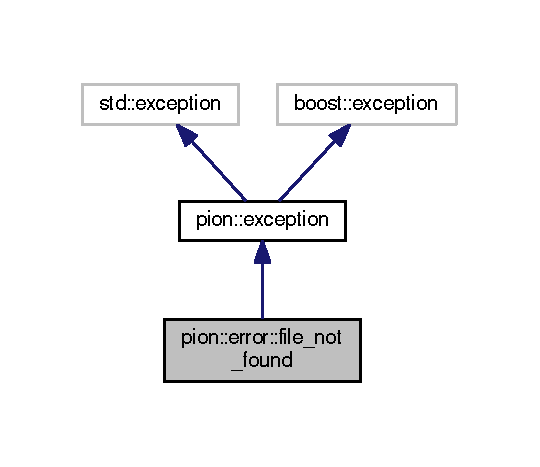
\includegraphics[width=259pt]{classpion_1_1error_1_1file__not__found__inherit__graph}
\end{center}
\end{figure}


Collaboration diagram for pion\-:\-:error\-:\-:file\-\_\-not\-\_\-found\-:
\nopagebreak
\begin{figure}[H]
\begin{center}
\leavevmode
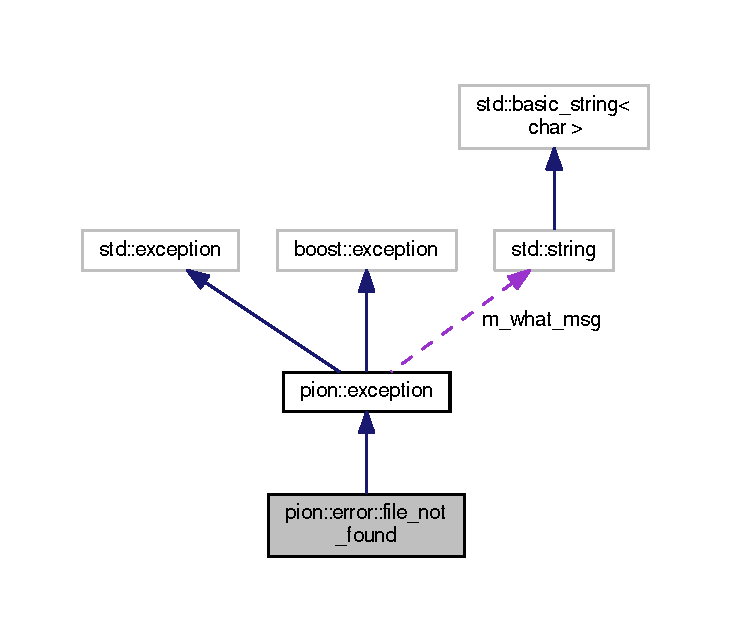
\includegraphics[width=350pt]{classpion_1_1error_1_1file__not__found__coll__graph}
\end{center}
\end{figure}
\subsection*{Additional Inherited Members}


\subsection{Detailed Description}
exception thrown if a file is not found 

The documentation for this class was generated from the following file\-:\begin{DoxyCompactItemize}
\item 
include/pion/\hyperlink{error_8hpp}{error.\-hpp}\end{DoxyCompactItemize}

\hypertarget{structpion_1_1iequal__to}{\section{pion\-:\-:iequal\-\_\-to Struct Reference}
\label{structpion_1_1iequal__to}\index{pion\-::iequal\-\_\-to@{pion\-::iequal\-\_\-to}}
}


{\ttfamily \#include $<$hash\-\_\-map.\-hpp$>$}



Inheritance diagram for pion\-:\-:iequal\-\_\-to\-:
\nopagebreak
\begin{figure}[H]
\begin{center}
\leavevmode
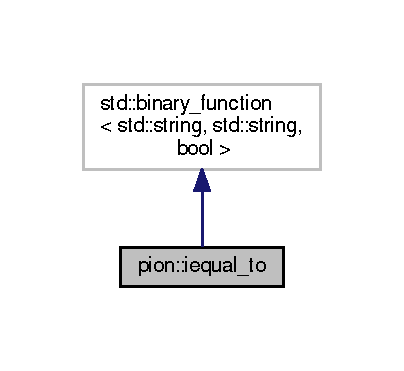
\includegraphics[width=194pt]{structpion_1_1iequal__to__inherit__graph}
\end{center}
\end{figure}


Collaboration diagram for pion\-:\-:iequal\-\_\-to\-:
\nopagebreak
\begin{figure}[H]
\begin{center}
\leavevmode
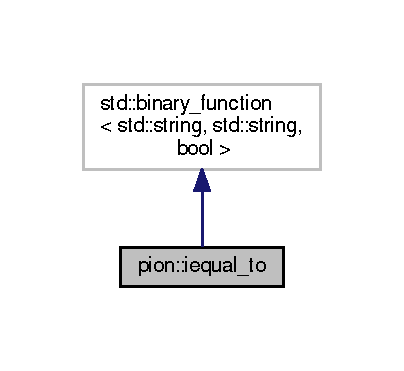
\includegraphics[width=194pt]{structpion_1_1iequal__to__coll__graph}
\end{center}
\end{figure}
\subsection*{Public Member Functions}
\begin{DoxyCompactItemize}
\item 
bool \hyperlink{structpion_1_1iequal__to_abdbf26bf08c7d62d25d76968558b4818}{operator()} (std\-::string const \&x, std\-::string const \&y) const 
\end{DoxyCompactItemize}


\subsection{Detailed Description}
case insensitive string equality predicate copied from boost.\-unordered hash\-\_\-equality documentation \href{http://www.boost.org/doc/libs/1_50_0/doc/html/unordered/hash_equality.html}{\tt http\-://www.\-boost.\-org/doc/libs/1\-\_\-50\-\_\-0/doc/html/unordered/hash\-\_\-equality.\-html} 

\subsection{Member Function Documentation}
\hypertarget{structpion_1_1iequal__to_abdbf26bf08c7d62d25d76968558b4818}{\index{pion\-::iequal\-\_\-to@{pion\-::iequal\-\_\-to}!operator()@{operator()}}
\index{operator()@{operator()}!pion::iequal_to@{pion\-::iequal\-\_\-to}}
\subsubsection[{operator()}]{\setlength{\rightskip}{0pt plus 5cm}bool pion\-::iequal\-\_\-to\-::operator() (
\begin{DoxyParamCaption}
\item[{std\-::string const \&}]{x, }
\item[{std\-::string const \&}]{y}
\end{DoxyParamCaption}
) const\hspace{0.3cm}{\ttfamily [inline]}}}\label{structpion_1_1iequal__to_abdbf26bf08c7d62d25d76968558b4818}


The documentation for this struct was generated from the following file\-:\begin{DoxyCompactItemize}
\item 
include/pion/\hyperlink{hash__map_8hpp}{hash\-\_\-map.\-hpp}\end{DoxyCompactItemize}

\hypertarget{structpion_1_1ihash}{\section{pion\-:\-:ihash Struct Reference}
\label{structpion_1_1ihash}\index{pion\-::ihash@{pion\-::ihash}}
}


{\ttfamily \#include $<$hash\-\_\-map.\-hpp$>$}



Inheritance diagram for pion\-:\-:ihash\-:
\nopagebreak
\begin{figure}[H]
\begin{center}
\leavevmode
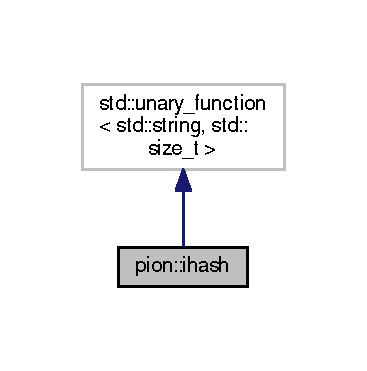
\includegraphics[width=176pt]{structpion_1_1ihash__inherit__graph}
\end{center}
\end{figure}


Collaboration diagram for pion\-:\-:ihash\-:
\nopagebreak
\begin{figure}[H]
\begin{center}
\leavevmode
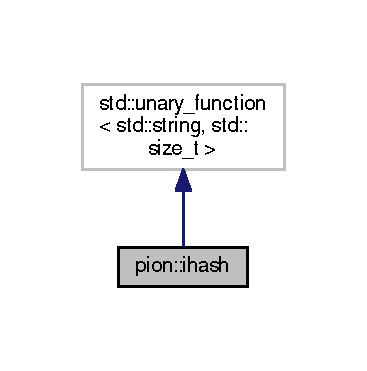
\includegraphics[width=176pt]{structpion_1_1ihash__coll__graph}
\end{center}
\end{figure}
\subsection*{Public Member Functions}
\begin{DoxyCompactItemize}
\item 
std\-::size\-\_\-t \hyperlink{structpion_1_1ihash_a9def756411120d3503edb9fd84ca67b7}{operator()} (std\-::string const \&x) const 
\end{DoxyCompactItemize}


\subsection{Detailed Description}
case insensitive hash generic function copied from boost.\-unordered hash\-\_\-equality documentation \href{http://www.boost.org/doc/libs/1_50_0/doc/html/unordered/hash_equality.html}{\tt http\-://www.\-boost.\-org/doc/libs/1\-\_\-50\-\_\-0/doc/html/unordered/hash\-\_\-equality.\-html} 

\subsection{Member Function Documentation}
\hypertarget{structpion_1_1ihash_a9def756411120d3503edb9fd84ca67b7}{\index{pion\-::ihash@{pion\-::ihash}!operator()@{operator()}}
\index{operator()@{operator()}!pion::ihash@{pion\-::ihash}}
\subsubsection[{operator()}]{\setlength{\rightskip}{0pt plus 5cm}std\-::size\-\_\-t pion\-::ihash\-::operator() (
\begin{DoxyParamCaption}
\item[{std\-::string const \&}]{x}
\end{DoxyParamCaption}
) const\hspace{0.3cm}{\ttfamily [inline]}}}\label{structpion_1_1ihash_a9def756411120d3503edb9fd84ca67b7}


The documentation for this struct was generated from the following file\-:\begin{DoxyCompactItemize}
\item 
include/pion/\hyperlink{hash__map_8hpp}{hash\-\_\-map.\-hpp}\end{DoxyCompactItemize}

\hypertarget{structpion_1_1logger}{\section{pion\-:\-:logger Struct Reference}
\label{structpion_1_1logger}\index{pion\-::logger@{pion\-::logger}}
}


{\ttfamily \#include $<$logger.\-hpp$>$}



Collaboration diagram for pion\-:\-:logger\-:
\nopagebreak
\begin{figure}[H]
\begin{center}
\leavevmode
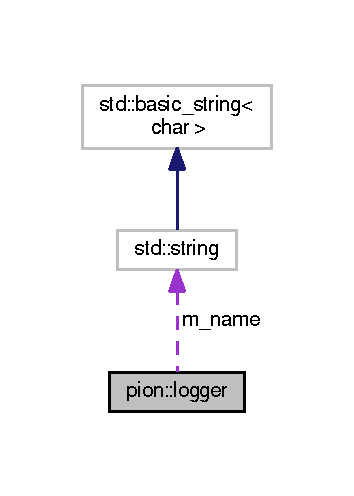
\includegraphics[width=170pt]{structpion_1_1logger__coll__graph}
\end{center}
\end{figure}
\subsection*{Public Types}
\begin{DoxyCompactItemize}
\item 
enum \hyperlink{structpion_1_1logger_a028e0caa7e4d190f0bbf629cd15456b8}{log\-\_\-priority\-\_\-type} \{ \\*
\hyperlink{structpion_1_1logger_a028e0caa7e4d190f0bbf629cd15456b8a36ae33c70511f0e2755ad24b009cd378}{L\-O\-G\-\_\-\-L\-E\-V\-E\-L\-\_\-\-D\-E\-B\-U\-G}, 
\hyperlink{structpion_1_1logger_a028e0caa7e4d190f0bbf629cd15456b8a469a91269377b34699eb188ca935dade}{L\-O\-G\-\_\-\-L\-E\-V\-E\-L\-\_\-\-I\-N\-F\-O}, 
\hyperlink{structpion_1_1logger_a028e0caa7e4d190f0bbf629cd15456b8aa53e46352ecd58083e2a70b5c37fc445}{L\-O\-G\-\_\-\-L\-E\-V\-E\-L\-\_\-\-W\-A\-R\-N}, 
\hyperlink{structpion_1_1logger_a028e0caa7e4d190f0bbf629cd15456b8a54e5ff73e35f679b488ed307d0d1ad99}{L\-O\-G\-\_\-\-L\-E\-V\-E\-L\-\_\-\-E\-R\-R\-O\-R}, 
\\*
\hyperlink{structpion_1_1logger_a028e0caa7e4d190f0bbf629cd15456b8aa3d4b8849e02f23d00e081703280a9e7}{L\-O\-G\-\_\-\-L\-E\-V\-E\-L\-\_\-\-F\-A\-T\-A\-L}
 \}
\end{DoxyCompactItemize}
\subsection*{Public Member Functions}
\begin{DoxyCompactItemize}
\item 
\hyperlink{structpion_1_1logger_abcd0ce04339a55c7268b4009c2a7a60c}{$\sim$logger} ()
\item 
\hyperlink{structpion_1_1logger_a4ea34e7e8f534ce97e288a2753afccf3}{logger} (void)
\item 
\hyperlink{structpion_1_1logger_a3b7ea2992e65a6a35f25bde03ea3be6e}{logger} (const std\-::string \&name)
\item 
\hyperlink{structpion_1_1logger_a6a68a76812570e28a2e98c60b9d7eb0f}{logger} (const \hyperlink{structpion_1_1logger}{logger} \&p)
\end{DoxyCompactItemize}
\subsection*{Static Public Member Functions}
\begin{DoxyCompactItemize}
\item 
static void \hyperlink{structpion_1_1logger_a2e9f33f545c83e3c6f59df3e067b9181}{shutdown} ()
\end{DoxyCompactItemize}
\subsection*{Public Attributes}
\begin{DoxyCompactItemize}
\item 
std\-::string \hyperlink{structpion_1_1logger_a4093c40a7d1be8af9a0106b0751ed68e}{m\-\_\-name}
\end{DoxyCompactItemize}
\subsection*{Static Public Attributes}
\begin{DoxyCompactItemize}
\item 
static \hyperlink{structpion_1_1logger_a028e0caa7e4d190f0bbf629cd15456b8}{log\-\_\-priority\-\_\-type} \hyperlink{structpion_1_1logger_a29cca3a109b06a74a38cd452c9c7ef70}{m\-\_\-priority}
\end{DoxyCompactItemize}


\subsection{Member Enumeration Documentation}
\hypertarget{structpion_1_1logger_a028e0caa7e4d190f0bbf629cd15456b8}{\index{pion\-::logger@{pion\-::logger}!log\-\_\-priority\-\_\-type@{log\-\_\-priority\-\_\-type}}
\index{log\-\_\-priority\-\_\-type@{log\-\_\-priority\-\_\-type}!pion::logger@{pion\-::logger}}
\subsubsection[{log\-\_\-priority\-\_\-type}]{\setlength{\rightskip}{0pt plus 5cm}enum {\bf pion\-::logger\-::log\-\_\-priority\-\_\-type}}}\label{structpion_1_1logger_a028e0caa7e4d190f0bbf629cd15456b8}
\begin{Desc}
\item[Enumerator]\par
\begin{description}
\index{L\-O\-G\-\_\-\-L\-E\-V\-E\-L\-\_\-\-D\-E\-B\-U\-G@{L\-O\-G\-\_\-\-L\-E\-V\-E\-L\-\_\-\-D\-E\-B\-U\-G}!pion\-::logger@{pion\-::logger}}\index{pion\-::logger@{pion\-::logger}!L\-O\-G\-\_\-\-L\-E\-V\-E\-L\-\_\-\-D\-E\-B\-U\-G@{L\-O\-G\-\_\-\-L\-E\-V\-E\-L\-\_\-\-D\-E\-B\-U\-G}}\item[{\em 
\hypertarget{structpion_1_1logger_a028e0caa7e4d190f0bbf629cd15456b8a36ae33c70511f0e2755ad24b009cd378}{L\-O\-G\-\_\-\-L\-E\-V\-E\-L\-\_\-\-D\-E\-B\-U\-G}\label{structpion_1_1logger_a028e0caa7e4d190f0bbf629cd15456b8a36ae33c70511f0e2755ad24b009cd378}
}]\index{L\-O\-G\-\_\-\-L\-E\-V\-E\-L\-\_\-\-I\-N\-F\-O@{L\-O\-G\-\_\-\-L\-E\-V\-E\-L\-\_\-\-I\-N\-F\-O}!pion\-::logger@{pion\-::logger}}\index{pion\-::logger@{pion\-::logger}!L\-O\-G\-\_\-\-L\-E\-V\-E\-L\-\_\-\-I\-N\-F\-O@{L\-O\-G\-\_\-\-L\-E\-V\-E\-L\-\_\-\-I\-N\-F\-O}}\item[{\em 
\hypertarget{structpion_1_1logger_a028e0caa7e4d190f0bbf629cd15456b8a469a91269377b34699eb188ca935dade}{L\-O\-G\-\_\-\-L\-E\-V\-E\-L\-\_\-\-I\-N\-F\-O}\label{structpion_1_1logger_a028e0caa7e4d190f0bbf629cd15456b8a469a91269377b34699eb188ca935dade}
}]\index{L\-O\-G\-\_\-\-L\-E\-V\-E\-L\-\_\-\-W\-A\-R\-N@{L\-O\-G\-\_\-\-L\-E\-V\-E\-L\-\_\-\-W\-A\-R\-N}!pion\-::logger@{pion\-::logger}}\index{pion\-::logger@{pion\-::logger}!L\-O\-G\-\_\-\-L\-E\-V\-E\-L\-\_\-\-W\-A\-R\-N@{L\-O\-G\-\_\-\-L\-E\-V\-E\-L\-\_\-\-W\-A\-R\-N}}\item[{\em 
\hypertarget{structpion_1_1logger_a028e0caa7e4d190f0bbf629cd15456b8aa53e46352ecd58083e2a70b5c37fc445}{L\-O\-G\-\_\-\-L\-E\-V\-E\-L\-\_\-\-W\-A\-R\-N}\label{structpion_1_1logger_a028e0caa7e4d190f0bbf629cd15456b8aa53e46352ecd58083e2a70b5c37fc445}
}]\index{L\-O\-G\-\_\-\-L\-E\-V\-E\-L\-\_\-\-E\-R\-R\-O\-R@{L\-O\-G\-\_\-\-L\-E\-V\-E\-L\-\_\-\-E\-R\-R\-O\-R}!pion\-::logger@{pion\-::logger}}\index{pion\-::logger@{pion\-::logger}!L\-O\-G\-\_\-\-L\-E\-V\-E\-L\-\_\-\-E\-R\-R\-O\-R@{L\-O\-G\-\_\-\-L\-E\-V\-E\-L\-\_\-\-E\-R\-R\-O\-R}}\item[{\em 
\hypertarget{structpion_1_1logger_a028e0caa7e4d190f0bbf629cd15456b8a54e5ff73e35f679b488ed307d0d1ad99}{L\-O\-G\-\_\-\-L\-E\-V\-E\-L\-\_\-\-E\-R\-R\-O\-R}\label{structpion_1_1logger_a028e0caa7e4d190f0bbf629cd15456b8a54e5ff73e35f679b488ed307d0d1ad99}
}]\index{L\-O\-G\-\_\-\-L\-E\-V\-E\-L\-\_\-\-F\-A\-T\-A\-L@{L\-O\-G\-\_\-\-L\-E\-V\-E\-L\-\_\-\-F\-A\-T\-A\-L}!pion\-::logger@{pion\-::logger}}\index{pion\-::logger@{pion\-::logger}!L\-O\-G\-\_\-\-L\-E\-V\-E\-L\-\_\-\-F\-A\-T\-A\-L@{L\-O\-G\-\_\-\-L\-E\-V\-E\-L\-\_\-\-F\-A\-T\-A\-L}}\item[{\em 
\hypertarget{structpion_1_1logger_a028e0caa7e4d190f0bbf629cd15456b8aa3d4b8849e02f23d00e081703280a9e7}{L\-O\-G\-\_\-\-L\-E\-V\-E\-L\-\_\-\-F\-A\-T\-A\-L}\label{structpion_1_1logger_a028e0caa7e4d190f0bbf629cd15456b8aa3d4b8849e02f23d00e081703280a9e7}
}]\end{description}
\end{Desc}


\subsection{Constructor \& Destructor Documentation}
\hypertarget{structpion_1_1logger_abcd0ce04339a55c7268b4009c2a7a60c}{\index{pion\-::logger@{pion\-::logger}!$\sim$logger@{$\sim$logger}}
\index{$\sim$logger@{$\sim$logger}!pion::logger@{pion\-::logger}}
\subsubsection[{$\sim$logger}]{\setlength{\rightskip}{0pt plus 5cm}pion\-::logger\-::$\sim$logger (
\begin{DoxyParamCaption}
{}
\end{DoxyParamCaption}
)\hspace{0.3cm}{\ttfamily [inline]}}}\label{structpion_1_1logger_abcd0ce04339a55c7268b4009c2a7a60c}
\hypertarget{structpion_1_1logger_a4ea34e7e8f534ce97e288a2753afccf3}{\index{pion\-::logger@{pion\-::logger}!logger@{logger}}
\index{logger@{logger}!pion::logger@{pion\-::logger}}
\subsubsection[{logger}]{\setlength{\rightskip}{0pt plus 5cm}pion\-::logger\-::logger (
\begin{DoxyParamCaption}
\item[{void}]{}
\end{DoxyParamCaption}
)\hspace{0.3cm}{\ttfamily [inline]}}}\label{structpion_1_1logger_a4ea34e7e8f534ce97e288a2753afccf3}
\hypertarget{structpion_1_1logger_a3b7ea2992e65a6a35f25bde03ea3be6e}{\index{pion\-::logger@{pion\-::logger}!logger@{logger}}
\index{logger@{logger}!pion::logger@{pion\-::logger}}
\subsubsection[{logger}]{\setlength{\rightskip}{0pt plus 5cm}pion\-::logger\-::logger (
\begin{DoxyParamCaption}
\item[{const std\-::string \&}]{name}
\end{DoxyParamCaption}
)\hspace{0.3cm}{\ttfamily [inline]}}}\label{structpion_1_1logger_a3b7ea2992e65a6a35f25bde03ea3be6e}
\hypertarget{structpion_1_1logger_a6a68a76812570e28a2e98c60b9d7eb0f}{\index{pion\-::logger@{pion\-::logger}!logger@{logger}}
\index{logger@{logger}!pion::logger@{pion\-::logger}}
\subsubsection[{logger}]{\setlength{\rightskip}{0pt plus 5cm}pion\-::logger\-::logger (
\begin{DoxyParamCaption}
\item[{const {\bf logger} \&}]{p}
\end{DoxyParamCaption}
)\hspace{0.3cm}{\ttfamily [inline]}}}\label{structpion_1_1logger_a6a68a76812570e28a2e98c60b9d7eb0f}


\subsection{Member Function Documentation}
\hypertarget{structpion_1_1logger_a2e9f33f545c83e3c6f59df3e067b9181}{\index{pion\-::logger@{pion\-::logger}!shutdown@{shutdown}}
\index{shutdown@{shutdown}!pion::logger@{pion\-::logger}}
\subsubsection[{shutdown}]{\setlength{\rightskip}{0pt plus 5cm}static void pion\-::logger\-::shutdown (
\begin{DoxyParamCaption}
{}
\end{DoxyParamCaption}
)\hspace{0.3cm}{\ttfamily [inline]}, {\ttfamily [static]}}}\label{structpion_1_1logger_a2e9f33f545c83e3c6f59df3e067b9181}


\subsection{Member Data Documentation}
\hypertarget{structpion_1_1logger_a4093c40a7d1be8af9a0106b0751ed68e}{\index{pion\-::logger@{pion\-::logger}!m\-\_\-name@{m\-\_\-name}}
\index{m\-\_\-name@{m\-\_\-name}!pion::logger@{pion\-::logger}}
\subsubsection[{m\-\_\-name}]{\setlength{\rightskip}{0pt plus 5cm}std\-::string pion\-::logger\-::m\-\_\-name}}\label{structpion_1_1logger_a4093c40a7d1be8af9a0106b0751ed68e}
\hypertarget{structpion_1_1logger_a29cca3a109b06a74a38cd452c9c7ef70}{\index{pion\-::logger@{pion\-::logger}!m\-\_\-priority@{m\-\_\-priority}}
\index{m\-\_\-priority@{m\-\_\-priority}!pion::logger@{pion\-::logger}}
\subsubsection[{m\-\_\-priority}]{\setlength{\rightskip}{0pt plus 5cm}{\bf log\-\_\-priority\-\_\-type} pion\-::logger\-::m\-\_\-priority\hspace{0.3cm}{\ttfamily [static]}}}\label{structpion_1_1logger_a29cca3a109b06a74a38cd452c9c7ef70}


The documentation for this struct was generated from the following file\-:\begin{DoxyCompactItemize}
\item 
include/pion/\hyperlink{logger_8hpp}{logger.\-hpp}\end{DoxyCompactItemize}

\hypertarget{classpion_1_1plugin__manager_1_1map__type}{\section{pion\-:\-:plugin\-\_\-manager$<$ Plugin\-Type $>$\-:\-:map\-\_\-type Class Reference}
\label{classpion_1_1plugin__manager_1_1map__type}\index{pion\-::plugin\-\_\-manager$<$ Plugin\-Type $>$\-::map\-\_\-type@{pion\-::plugin\-\_\-manager$<$ Plugin\-Type $>$\-::map\-\_\-type}}
}


data type that maps identifiers to plug-\/in objects  




{\ttfamily \#include $<$plugin\-\_\-manager.\-hpp$>$}



Inheritance diagram for pion\-:\-:plugin\-\_\-manager$<$ Plugin\-Type $>$\-:\-:map\-\_\-type\-:
\nopagebreak
\begin{figure}[H]
\begin{center}
\leavevmode
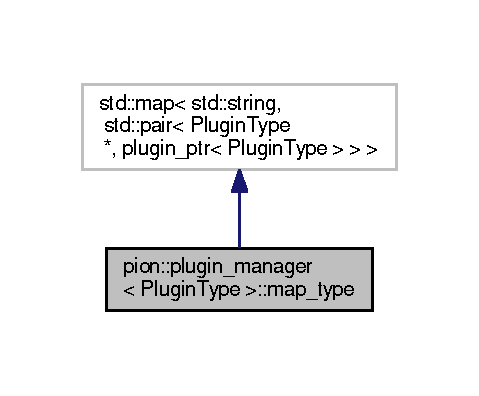
\includegraphics[width=230pt]{classpion_1_1plugin__manager_1_1map__type__inherit__graph}
\end{center}
\end{figure}


Collaboration diagram for pion\-:\-:plugin\-\_\-manager$<$ Plugin\-Type $>$\-:\-:map\-\_\-type\-:
\nopagebreak
\begin{figure}[H]
\begin{center}
\leavevmode
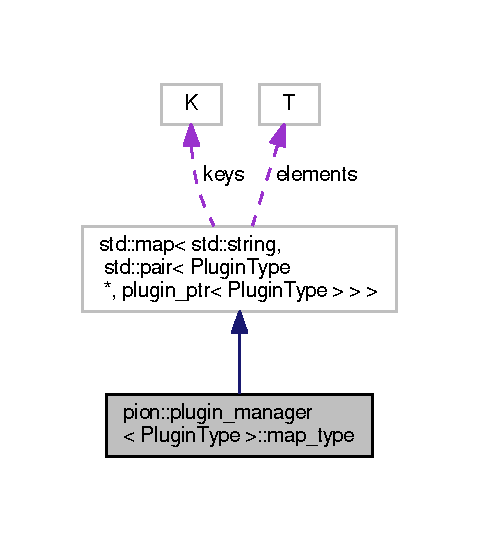
\includegraphics[width=230pt]{classpion_1_1plugin__manager_1_1map__type__coll__graph}
\end{center}
\end{figure}
\subsection*{Public Member Functions}
\begin{DoxyCompactItemize}
\item 
void \hyperlink{classpion_1_1plugin__manager_1_1map__type_a68c8fa315ba4a7ff7bb81a14e362dff1}{clear} (void)
\item 
virtual \hyperlink{classpion_1_1plugin__manager_1_1map__type_aebb882207cac1e5e98d09f6a74c2a2cb}{$\sim$map\-\_\-type} ()
\item 
\hyperlink{classpion_1_1plugin__manager_1_1map__type_a5bcef449c5faa390bcbd44c1df613206}{map\-\_\-type} (void)
\end{DoxyCompactItemize}


\subsection{Detailed Description}
\subsubsection*{template$<$typename Plugin\-Type$>$class pion\-::plugin\-\_\-manager$<$ Plugin\-Type $>$\-::map\-\_\-type}

data type that maps identifiers to plug-\/in objects 

\subsection{Constructor \& Destructor Documentation}
\hypertarget{classpion_1_1plugin__manager_1_1map__type_aebb882207cac1e5e98d09f6a74c2a2cb}{\index{pion\-::plugin\-\_\-manager\-::map\-\_\-type@{pion\-::plugin\-\_\-manager\-::map\-\_\-type}!$\sim$map\-\_\-type@{$\sim$map\-\_\-type}}
\index{$\sim$map\-\_\-type@{$\sim$map\-\_\-type}!pion::plugin_manager::map_type@{pion\-::plugin\-\_\-manager\-::map\-\_\-type}}
\subsubsection[{$\sim$map\-\_\-type}]{\setlength{\rightskip}{0pt plus 5cm}template$<$typename Plugin\-Type$>$ virtual {\bf pion\-::plugin\-\_\-manager}$<$ Plugin\-Type $>$\-::map\-\_\-type\-::$\sim$map\-\_\-type (
\begin{DoxyParamCaption}
{}
\end{DoxyParamCaption}
)\hspace{0.3cm}{\ttfamily [inline]}, {\ttfamily [virtual]}}}\label{classpion_1_1plugin__manager_1_1map__type_aebb882207cac1e5e98d09f6a74c2a2cb}


References pion\-::plugin\-\_\-manager$<$ Plugin\-Type $>$\-::map\-\_\-type\-::clear().

\hypertarget{classpion_1_1plugin__manager_1_1map__type_a5bcef449c5faa390bcbd44c1df613206}{\index{pion\-::plugin\-\_\-manager\-::map\-\_\-type@{pion\-::plugin\-\_\-manager\-::map\-\_\-type}!map\-\_\-type@{map\-\_\-type}}
\index{map\-\_\-type@{map\-\_\-type}!pion::plugin_manager::map_type@{pion\-::plugin\-\_\-manager\-::map\-\_\-type}}
\subsubsection[{map\-\_\-type}]{\setlength{\rightskip}{0pt plus 5cm}template$<$typename Plugin\-Type$>$ {\bf pion\-::plugin\-\_\-manager}$<$ Plugin\-Type $>$\-::map\-\_\-type\-::map\-\_\-type (
\begin{DoxyParamCaption}
\item[{void}]{}
\end{DoxyParamCaption}
)\hspace{0.3cm}{\ttfamily [inline]}}}\label{classpion_1_1plugin__manager_1_1map__type_a5bcef449c5faa390bcbd44c1df613206}


\subsection{Member Function Documentation}
\hypertarget{classpion_1_1plugin__manager_1_1map__type_a68c8fa315ba4a7ff7bb81a14e362dff1}{\index{pion\-::plugin\-\_\-manager\-::map\-\_\-type@{pion\-::plugin\-\_\-manager\-::map\-\_\-type}!clear@{clear}}
\index{clear@{clear}!pion::plugin_manager::map_type@{pion\-::plugin\-\_\-manager\-::map\-\_\-type}}
\subsubsection[{clear}]{\setlength{\rightskip}{0pt plus 5cm}template$<$typename Plugin\-Type$>$ void {\bf pion\-::plugin\-\_\-manager}$<$ Plugin\-Type $>$\-::map\-\_\-type\-::clear (
\begin{DoxyParamCaption}
\item[{void}]{}
\end{DoxyParamCaption}
)\hspace{0.3cm}{\ttfamily [inline]}}}\label{classpion_1_1plugin__manager_1_1map__type_a68c8fa315ba4a7ff7bb81a14e362dff1}


References pion\-::plugin\-\_\-manager$<$ Plugin\-Type $>$\-::empty().



Referenced by pion\-::plugin\-\_\-manager$<$ http\-::plugin\-\_\-service $>$\-::clear(), and pion\-::plugin\-\_\-manager$<$ Plugin\-Type $>$\-::map\-\_\-type\-::$\sim$map\-\_\-type().



The documentation for this class was generated from the following file\-:\begin{DoxyCompactItemize}
\item 
include/pion/\hyperlink{plugin__manager_8hpp}{plugin\-\_\-manager.\-hpp}\end{DoxyCompactItemize}

\hypertarget{classpion_1_1http_1_1message}{\section{pion\-:\-:http\-:\-:message Class Reference}
\label{classpion_1_1http_1_1message}\index{pion\-::http\-::message@{pion\-::http\-::message}}
}


{\ttfamily \#include $<$message.\-hpp$>$}



Inheritance diagram for pion\-:\-:http\-:\-:message\-:
\nopagebreak
\begin{figure}[H]
\begin{center}
\leavevmode
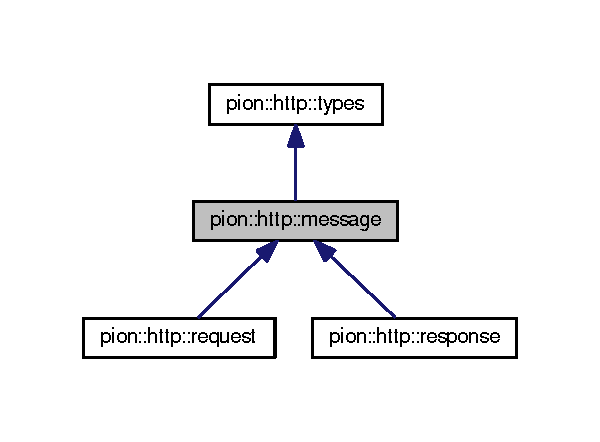
\includegraphics[width=288pt]{classpion_1_1http_1_1message__inherit__graph}
\end{center}
\end{figure}


Collaboration diagram for pion\-:\-:http\-:\-:message\-:
\nopagebreak
\begin{figure}[H]
\begin{center}
\leavevmode
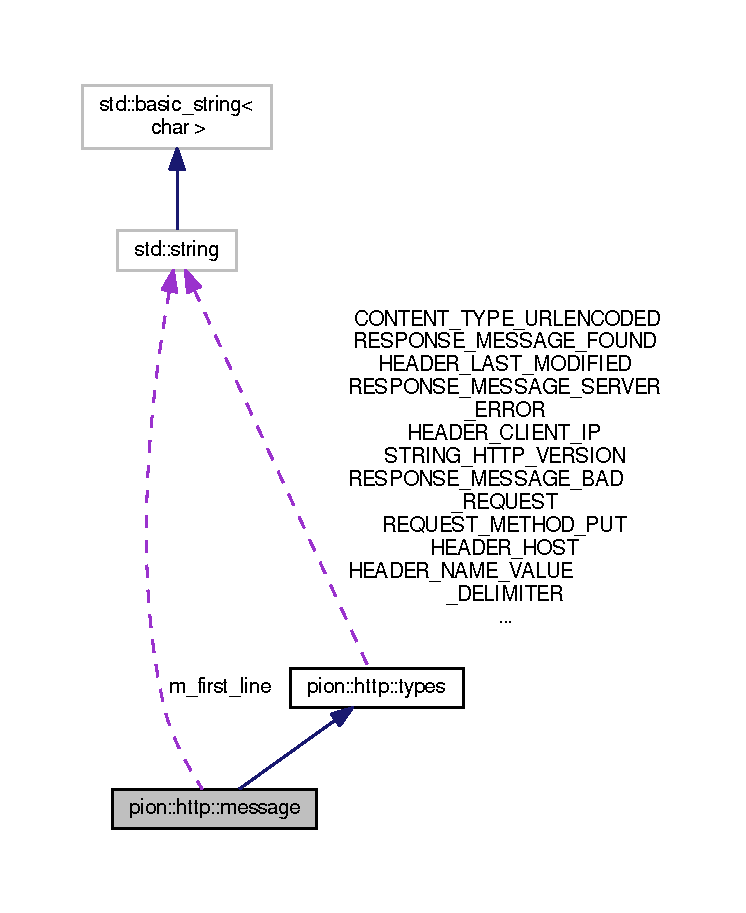
\includegraphics[width=350pt]{classpion_1_1http_1_1message__coll__graph}
\end{center}
\end{figure}
\subsection*{Classes}
\begin{DoxyCompactItemize}
\item 
class \hyperlink{classpion_1_1http_1_1message_1_1content__buffer__t}{content\-\_\-buffer\-\_\-t}
\begin{DoxyCompactList}\small\item\em a simple helper class used to manage a fixed-\/size payload content buffer \end{DoxyCompactList}\item 
struct \hyperlink{structpion_1_1http_1_1message_1_1receive__error__t}{receive\-\_\-error\-\_\-t}
\begin{DoxyCompactList}\small\item\em data type for library errors returned during \hyperlink{classpion_1_1http_1_1message_a7e3c3f1ea265f91b87a9e075234b5d31}{receive()} operations \end{DoxyCompactList}\end{DoxyCompactItemize}
\subsection*{Public Types}
\begin{DoxyCompactItemize}
\item 
enum \hyperlink{classpion_1_1http_1_1message_ab71e06f72cacb4945dbf84663b0420e9}{data\-\_\-status\-\_\-t} \{ \hyperlink{classpion_1_1http_1_1message_ab71e06f72cacb4945dbf84663b0420e9a857bcfd3cb3884033f73a22e9d5ade05}{S\-T\-A\-T\-U\-S\-\_\-\-N\-O\-N\-E}, 
\hyperlink{classpion_1_1http_1_1message_ab71e06f72cacb4945dbf84663b0420e9ab69b544af26550d7cf5b0a795078715c}{S\-T\-A\-T\-U\-S\-\_\-\-T\-R\-U\-N\-C\-A\-T\-E\-D}, 
\hyperlink{classpion_1_1http_1_1message_ab71e06f72cacb4945dbf84663b0420e9a4b310a8c8463d24ac0d8073eba11ef4a}{S\-T\-A\-T\-U\-S\-\_\-\-P\-A\-R\-T\-I\-A\-L}, 
\hyperlink{classpion_1_1http_1_1message_ab71e06f72cacb4945dbf84663b0420e9a5fd3c3fcefd1a51ee076e40708e32674}{S\-T\-A\-T\-U\-S\-\_\-\-O\-K}
 \}
\begin{DoxyCompactList}\small\item\em defines message data integrity status codes \end{DoxyCompactList}\item 
typedef std\-::vector\\*
$<$ boost\-::asio\-::const\-\_\-buffer $>$ \hyperlink{classpion_1_1http_1_1message_aacf9a6a7677c32e4ab764ac97d0b5e7b}{write\-\_\-buffers\-\_\-t}
\begin{DoxyCompactList}\small\item\em data type for I/\-O write buffers (these wrap existing data to be sent) \end{DoxyCompactList}\item 
typedef std\-::vector$<$ char $>$ \hyperlink{classpion_1_1http_1_1message_a4bcf1ea1d4e7a5637d04ae109adb5e46}{chunk\-\_\-cache\-\_\-t}
\begin{DoxyCompactList}\small\item\em used to cache chunked data \end{DoxyCompactList}\end{DoxyCompactItemize}
\subsection*{Public Member Functions}
\begin{DoxyCompactItemize}
\item 
\hyperlink{classpion_1_1http_1_1message_ad07a7f30359b9f44c9159f3f9a9db507}{message} (void)
\begin{DoxyCompactList}\small\item\em constructs a new H\-T\-T\-P message object \end{DoxyCompactList}\item 
\hyperlink{classpion_1_1http_1_1message_a576e849f9d4a138d4856c83ceb0c47a3}{message} (const \hyperlink{classpion_1_1http_1_1message}{message} \&http\-\_\-msg)
\begin{DoxyCompactList}\small\item\em copy constructor \end{DoxyCompactList}\item 
\hyperlink{classpion_1_1http_1_1message}{message} \& \hyperlink{classpion_1_1http_1_1message_a854b089e577498c9b01e5ec460595a35}{operator=} (const \hyperlink{classpion_1_1http_1_1message}{message} \&http\-\_\-msg)
\begin{DoxyCompactList}\small\item\em assignment operator \end{DoxyCompactList}\item 
virtual \hyperlink{classpion_1_1http_1_1message_ac71ae21f149f7d74b2bdee1bf1149ead}{$\sim$message} ()
\begin{DoxyCompactList}\small\item\em virtual destructor \end{DoxyCompactList}\item 
virtual void \hyperlink{classpion_1_1http_1_1message_af13279269cf1e00ae4fc5091c1c7cae5}{clear} (void)
\begin{DoxyCompactList}\small\item\em clears all message data \end{DoxyCompactList}\item 
virtual bool \hyperlink{classpion_1_1http_1_1message_a08bd257bd46e7a42b64bbc4482f28363}{is\-\_\-content\-\_\-length\-\_\-implied} (void) const =0
\begin{DoxyCompactList}\small\item\em should return true if the content length can be implied without headers \end{DoxyCompactList}\item 
bool \hyperlink{classpion_1_1http_1_1message_a52850e6fe48b141f46662c83d4edbbf5}{is\-\_\-valid} (void) const 
\begin{DoxyCompactList}\small\item\em returns true if the message is valid \end{DoxyCompactList}\item 
bool \hyperlink{classpion_1_1http_1_1message_a42ea3cfa8633a99a9c517afe2db00a1a}{get\-\_\-chunks\-\_\-supported} (void) const 
\begin{DoxyCompactList}\small\item\em returns true if chunked transfer encodings are supported \end{DoxyCompactList}\item 
boost\-::asio\-::ip\-::address \& \hyperlink{classpion_1_1http_1_1message_a42fdde8d94227c6d08d475c5ed8a6388}{get\-\_\-remote\-\_\-ip} (void)
\begin{DoxyCompactList}\small\item\em returns I\-P address of the remote endpoint \end{DoxyCompactList}\item 
boost\-::uint16\-\_\-t \hyperlink{classpion_1_1http_1_1message_a6d36c13df002129d3044d9c34999161d}{get\-\_\-version\-\_\-major} (void) const 
\begin{DoxyCompactList}\small\item\em returns the major H\-T\-T\-P version number \end{DoxyCompactList}\item 
boost\-::uint16\-\_\-t \hyperlink{classpion_1_1http_1_1message_ac986c7014db695241db1823f17eda4cd}{get\-\_\-version\-\_\-minor} (void) const 
\begin{DoxyCompactList}\small\item\em returns the minor H\-T\-T\-P version number \end{DoxyCompactList}\item 
std\-::string \hyperlink{classpion_1_1http_1_1message_a0bb6e14bd27dc1b956bb74dcccc7ee27}{get\-\_\-version\-\_\-string} (void) const 
\begin{DoxyCompactList}\small\item\em returns a string representation of the H\-T\-T\-P version (i.\-e. \char`\"{}\-H\-T\-T\-P/1.\-1\char`\"{}) \end{DoxyCompactList}\item 
size\-\_\-t \hyperlink{classpion_1_1http_1_1message_a10606f8fd2efbe14d447ef8eb8731a54}{get\-\_\-content\-\_\-length} (void) const 
\begin{DoxyCompactList}\small\item\em returns the length of the payload content (in bytes) \end{DoxyCompactList}\item 
bool \hyperlink{classpion_1_1http_1_1message_a96264a238b04e1957c87ab7930a8023b}{is\-\_\-chunked} (void) const 
\begin{DoxyCompactList}\small\item\em returns true if the message content is chunked \end{DoxyCompactList}\item 
bool \hyperlink{classpion_1_1http_1_1message_a7229c3a00b35846cdb050fc2b9b6ec73}{is\-\_\-content\-\_\-buffer\-\_\-allocated} () const 
\begin{DoxyCompactList}\small\item\em returns true if buffer for content is allocated \end{DoxyCompactList}\item 
std\-::size\-\_\-t \hyperlink{classpion_1_1http_1_1message_a172346504faba36f73d7527551c199a2}{get\-\_\-content\-\_\-buffer\-\_\-size} () const 
\begin{DoxyCompactList}\small\item\em returns size of allocated buffer \end{DoxyCompactList}\item 
char $\ast$ \hyperlink{classpion_1_1http_1_1message_a60ddb1bd09afecdadc5e9c33c8c1de28}{get\-\_\-content} (void)
\begin{DoxyCompactList}\small\item\em returns a pointer to the payload content, or empty string if there is none \end{DoxyCompactList}\item 
const char $\ast$ \hyperlink{classpion_1_1http_1_1message_aa2363086d3f0c17a54ecebaef558b971}{get\-\_\-content} (void) const 
\begin{DoxyCompactList}\small\item\em returns a const pointer to the payload content, or empty string if there is none \end{DoxyCompactList}\item 
\hyperlink{classpion_1_1http_1_1message_a4bcf1ea1d4e7a5637d04ae109adb5e46}{chunk\-\_\-cache\-\_\-t} \& \hyperlink{classpion_1_1http_1_1message_aa672e8369ab07a212902a98f351805f3}{get\-\_\-chunk\-\_\-cache} (void)
\begin{DoxyCompactList}\small\item\em returns a reference to the chunk cache \end{DoxyCompactList}\item 
const std\-::string \& \hyperlink{classpion_1_1http_1_1message_ab9e2735d01890cd8e93f86390cd46969}{get\-\_\-header} (const std\-::string \&key) const 
\begin{DoxyCompactList}\small\item\em returns a value for the header if any are defined; otherwise, an empty string \end{DoxyCompactList}\item 
\hyperlink{namespacepion_a2cd31d7bbe0e98008bd4e6f135103c0e}{ihash\-\_\-multimap} \& \hyperlink{classpion_1_1http_1_1message_a8d067675e0396114e814ad688bed2b4f}{get\-\_\-headers} (void)
\begin{DoxyCompactList}\small\item\em returns a reference to the H\-T\-T\-P headers \end{DoxyCompactList}\item 
bool \hyperlink{classpion_1_1http_1_1message_ac6667e7a771b157e24858700b4777223}{has\-\_\-header} (const std\-::string \&key) const 
\begin{DoxyCompactList}\small\item\em returns true if at least one value for the header is defined \end{DoxyCompactList}\item 
const std\-::string \& \hyperlink{classpion_1_1http_1_1message_a735de2125e0b3c3a8caae7fad757cfc0}{get\-\_\-cookie} (const std\-::string \&key) const 
\item 
\hyperlink{namespacepion_a2cd31d7bbe0e98008bd4e6f135103c0e}{ihash\-\_\-multimap} \& \hyperlink{classpion_1_1http_1_1message_ab5e744890af0936eda97c21888bb4a2e}{get\-\_\-cookies} (void)
\begin{DoxyCompactList}\small\item\em returns the cookie parameters \end{DoxyCompactList}\item 
bool \hyperlink{classpion_1_1http_1_1message_af033e860c1f7295a6ef8eb5ea75f53e8}{has\-\_\-cookie} (const std\-::string \&key) const 
\item 
void \hyperlink{classpion_1_1http_1_1message_a0bc8756a9db916d5423dad19211de771}{add\-\_\-cookie} (const std\-::string \&key, const std\-::string \&value)
\item 
void \hyperlink{classpion_1_1http_1_1message_a1bfed0c1dc6a76384798c51ae74ea2da}{change\-\_\-cookie} (const std\-::string \&key, const std\-::string \&value)
\item 
void \hyperlink{classpion_1_1http_1_1message_a79e4153703ae62a1b8b0585510d032fd}{delete\-\_\-cookie} (const std\-::string \&key)
\item 
const std\-::string \& \hyperlink{classpion_1_1http_1_1message_ad9c43932bae03916ad193c257a7ec6c8}{get\-\_\-first\-\_\-line} (void) const 
\begin{DoxyCompactList}\small\item\em returns a string containing the first line for the H\-T\-T\-P message \end{DoxyCompactList}\item 
bool \hyperlink{classpion_1_1http_1_1message_a0ab661db865a6d018e8487a1b4f6932b}{has\-\_\-missing\-\_\-packets} () const 
\begin{DoxyCompactList}\small\item\em true if there were missing packets \end{DoxyCompactList}\item 
void \hyperlink{classpion_1_1http_1_1message_ac0749dac4643586e3925d73782840b26}{set\-\_\-missing\-\_\-packets} (bool new\-Val)
\begin{DoxyCompactList}\small\item\em set to true when missing packets detected \end{DoxyCompactList}\item 
bool \hyperlink{classpion_1_1http_1_1message_a52fd51aca9d5a37f41a0ad18d577ddec}{has\-\_\-data\-\_\-after\-\_\-missing\-\_\-packets} () const 
\begin{DoxyCompactList}\small\item\em true if more data seen after the missing packets \end{DoxyCompactList}\item 
void \hyperlink{classpion_1_1http_1_1message_af9081484fde89d5e8bdfcb689bebdeb1}{set\-\_\-data\-\_\-after\-\_\-missing\-\_\-packet} (bool new\-Val)
\item 
void \hyperlink{classpion_1_1http_1_1message_a24b208fd31a21a5bdb76a6ba8683321e}{set\-\_\-is\-\_\-valid} (bool b=true)
\begin{DoxyCompactList}\small\item\em sets whether or not the message is valid \end{DoxyCompactList}\item 
void \hyperlink{classpion_1_1http_1_1message_a524e682e0c1843d2bee6ad83c6b9e218}{set\-\_\-chunks\-\_\-supported} (bool b)
\begin{DoxyCompactList}\small\item\em set to true if chunked transfer encodings are supported \end{DoxyCompactList}\item 
void \hyperlink{classpion_1_1http_1_1message_a476f852158ecaefef8f3e93a84e1f76a}{set\-\_\-remote\-\_\-ip} (const boost\-::asio\-::ip\-::address \&ip)
\begin{DoxyCompactList}\small\item\em sets I\-P address of the remote endpoint \end{DoxyCompactList}\item 
void \hyperlink{classpion_1_1http_1_1message_aab454a1ce4eebd904b8ee7fff3dbe5d9}{set\-\_\-version\-\_\-major} (const boost\-::uint16\-\_\-t n)
\begin{DoxyCompactList}\small\item\em sets the major H\-T\-T\-P version number \end{DoxyCompactList}\item 
void \hyperlink{classpion_1_1http_1_1message_a311e93b0818ec735a4933e825a55c12e}{set\-\_\-version\-\_\-minor} (const boost\-::uint16\-\_\-t n)
\begin{DoxyCompactList}\small\item\em sets the minor H\-T\-T\-P version number \end{DoxyCompactList}\item 
void \hyperlink{classpion_1_1http_1_1message_a81612c01ac85ebe08b947b1f9cfc2a75}{set\-\_\-content\-\_\-length} (size\-\_\-t n)
\begin{DoxyCompactList}\small\item\em sets the length of the payload content (in bytes) \end{DoxyCompactList}\item 
void \hyperlink{classpion_1_1http_1_1message_af6cf5b229cacaaec5ea2bac0df53e199}{set\-\_\-do\-\_\-not\-\_\-send\-\_\-content\-\_\-length} (void)
\begin{DoxyCompactList}\small\item\em if called, the content-\/length will not be sent in the H\-T\-T\-P headers \end{DoxyCompactList}\item 
\hyperlink{classpion_1_1http_1_1message_ab71e06f72cacb4945dbf84663b0420e9}{data\-\_\-status\-\_\-t} \hyperlink{classpion_1_1http_1_1message_aabb2581095e035b5b274ee88442ad9ed}{get\-\_\-status} () const 
\begin{DoxyCompactList}\small\item\em return the data receival status \end{DoxyCompactList}\item 
void \hyperlink{classpion_1_1http_1_1message_ad24b94c3ad437b2044c2658fa34bd78d}{set\-\_\-status} (\hyperlink{classpion_1_1http_1_1message_ab71e06f72cacb4945dbf84663b0420e9}{data\-\_\-status\-\_\-t} new\-Val)
\item 
void \hyperlink{classpion_1_1http_1_1message_a6a7a6a5114da843c033283a6c1db48aa}{update\-\_\-content\-\_\-length\-\_\-using\-\_\-header} (void)
\begin{DoxyCompactList}\small\item\em sets the length of the payload content using the Content-\/\-Length header \end{DoxyCompactList}\item 
void \hyperlink{classpion_1_1http_1_1message_a8118770f69c9a479f3f5dcbc58d6d644}{update\-\_\-transfer\-\_\-encoding\-\_\-using\-\_\-header} (void)
\begin{DoxyCompactList}\small\item\em sets the transfer coding using the Transfer-\/\-Encoding header \end{DoxyCompactList}\item 
char $\ast$ \hyperlink{classpion_1_1http_1_1message_a468f42e5bc2866d9c93138e3a4cec31b}{create\-\_\-content\-\_\-buffer} (void)
\item 
void \hyperlink{classpion_1_1http_1_1message_a3600676865fc813897e0ed45b58e5600}{set\-\_\-content} (const std\-::string \&content)
\begin{DoxyCompactList}\small\item\em resets payload content to match the value of a string \end{DoxyCompactList}\item 
void \hyperlink{classpion_1_1http_1_1message_a33567717927344a33bc8332ad3a391a6}{clear\-\_\-content} (void)
\begin{DoxyCompactList}\small\item\em clears payload content buffer \end{DoxyCompactList}\item 
void \hyperlink{classpion_1_1http_1_1message_add4f889bb2d22e163556c2fd5fd993a8}{set\-\_\-content\-\_\-type} (const std\-::string \&type)
\begin{DoxyCompactList}\small\item\em sets the content type for the message payload \end{DoxyCompactList}\item 
void \hyperlink{classpion_1_1http_1_1message_a115c9657c4933f034dcf2f4ce7bd55f0}{add\-\_\-header} (const std\-::string \&key, const std\-::string \&value)
\begin{DoxyCompactList}\small\item\em adds a value for the H\-T\-T\-P header named key \end{DoxyCompactList}\item 
void \hyperlink{classpion_1_1http_1_1message_aa1643164e7f60bae1b640d55735a4728}{change\-\_\-header} (const std\-::string \&key, const std\-::string \&value)
\begin{DoxyCompactList}\small\item\em changes the value for the H\-T\-T\-P header named key \end{DoxyCompactList}\item 
void \hyperlink{classpion_1_1http_1_1message_a070ef742af75674725da392c25774884}{delete\-\_\-header} (const std\-::string \&key)
\begin{DoxyCompactList}\small\item\em removes all values for the H\-T\-T\-P header named key \end{DoxyCompactList}\item 
bool \hyperlink{classpion_1_1http_1_1message_ab0aa463a1327eac0d73ff6ab62ca3891}{check\-\_\-keep\-\_\-alive} (void) const 
\begin{DoxyCompactList}\small\item\em returns true if the H\-T\-T\-P connection may be kept alive \end{DoxyCompactList}\item 
void \hyperlink{classpion_1_1http_1_1message_a668182618dfc614ddbe6c1af26552568}{prepare\-\_\-buffers\-\_\-for\-\_\-send} (\hyperlink{classpion_1_1http_1_1message_aacf9a6a7677c32e4ab764ac97d0b5e7b}{write\-\_\-buffers\-\_\-t} \&write\-\_\-buffers, const bool keep\-\_\-alive, const bool using\-\_\-chunks)
\item 
std\-::size\-\_\-t \hyperlink{classpion_1_1http_1_1message_ab90f91badb0f98f900a7624418781bea}{send} (\hyperlink{classpion_1_1tcp_1_1connection}{tcp\-::connection} \&tcp\-\_\-conn, boost\-::system\-::error\-\_\-code \&ec, bool headers\-\_\-only=false)
\item 
std\-::size\-\_\-t \hyperlink{classpion_1_1http_1_1message_a7e3c3f1ea265f91b87a9e075234b5d31}{receive} (\hyperlink{classpion_1_1tcp_1_1connection}{tcp\-::connection} \&tcp\-\_\-conn, boost\-::system\-::error\-\_\-code \&ec, \hyperlink{classpion_1_1http_1_1parser}{parser} \&http\-\_\-parser)
\item 
std\-::size\-\_\-t \hyperlink{classpion_1_1http_1_1message_a029d3c6260deabf91fdcc9f1f0157268}{receive} (\hyperlink{classpion_1_1tcp_1_1connection}{tcp\-::connection} \&tcp\-\_\-conn, boost\-::system\-::error\-\_\-code \&ec, bool headers\-\_\-only=false, std\-::size\-\_\-t max\-\_\-content\-\_\-length=static\-\_\-cast$<$ size\-\_\-t $>$(-\/1))
\item 
std\-::size\-\_\-t \hyperlink{classpion_1_1http_1_1message_a4a3911ad03031a1ddacfa4cedeb125a2}{write} (std\-::ostream \&out, boost\-::system\-::error\-\_\-code \&ec, bool headers\-\_\-only=false)
\item 
std\-::size\-\_\-t \hyperlink{classpion_1_1http_1_1message_a7b67f3e8303d838bb5d379ab72a35e2d}{read} (std\-::istream \&in, boost\-::system\-::error\-\_\-code \&ec, \hyperlink{classpion_1_1http_1_1parser}{parser} \&http\-\_\-parser)
\item 
std\-::size\-\_\-t \hyperlink{classpion_1_1http_1_1message_ae99b6c39dd1b878520125f7037c035de}{read} (std\-::istream \&in, boost\-::system\-::error\-\_\-code \&ec, bool headers\-\_\-only=false, std\-::size\-\_\-t max\-\_\-content\-\_\-length=static\-\_\-cast$<$ size\-\_\-t $>$(-\/1))
\item 
void \hyperlink{classpion_1_1http_1_1message_aeffca5e2173be2b83f38b630d07f4bfd}{concatenate\-\_\-chunks} (void)
\end{DoxyCompactItemize}
\subsection*{Protected Member Functions}
\begin{DoxyCompactItemize}
\item 
void \hyperlink{classpion_1_1http_1_1message_a1addd3b90c3b048c895f9723371f329f}{prepare\-\_\-headers\-\_\-for\-\_\-send} (const bool keep\-\_\-alive, const bool using\-\_\-chunks)
\item 
void \hyperlink{classpion_1_1http_1_1message_a3184733c3a21b8aa44d8f301eaf52697}{append\-\_\-headers} (\hyperlink{classpion_1_1http_1_1message_aacf9a6a7677c32e4ab764ac97d0b5e7b}{write\-\_\-buffers\-\_\-t} \&write\-\_\-buffers)
\item 
virtual void \hyperlink{classpion_1_1http_1_1message_a532d475ab2dfdcdb969445902fad2e6f}{append\-\_\-cookie\-\_\-headers} (void)
\begin{DoxyCompactList}\small\item\em appends H\-T\-T\-P headers for any cookies defined by the \href{http::message}{\tt http\-::message} \end{DoxyCompactList}\item 
void \hyperlink{classpion_1_1http_1_1message_ab47dc3343c9b2cbc7fdf8605e4b7d3b2}{clear\-\_\-first\-\_\-line} (void) const 
\item 
virtual void \hyperlink{classpion_1_1http_1_1message_a697a832ab0741d02ddecd8df8da0265d}{update\-\_\-first\-\_\-line} (void) const =0
\begin{DoxyCompactList}\small\item\em updates the string containing the first line for the H\-T\-T\-P message \end{DoxyCompactList}\end{DoxyCompactItemize}
\subsection*{Static Protected Member Functions}
\begin{DoxyCompactItemize}
\item 
{\footnotesize template$<$typename Dictionary\-Type $>$ }\\static const std\-::string \& \hyperlink{classpion_1_1http_1_1message_ad6e365382874be8f3e28df1234e3a3f7}{get\-\_\-value} (const Dictionary\-Type \&dict, const std\-::string \&key)
\item 
{\footnotesize template$<$typename Dictionary\-Type $>$ }\\static void \hyperlink{classpion_1_1http_1_1message_a40603cf88819b33abb4e56bb55dc61af}{change\-\_\-value} (Dictionary\-Type \&dict, const std\-::string \&key, const std\-::string \&value)
\item 
{\footnotesize template$<$typename Dictionary\-Type $>$ }\\static void \hyperlink{classpion_1_1http_1_1message_a6d07488a5fa36e1e90622d64179f7953}{delete\-\_\-value} (Dictionary\-Type \&dict, const std\-::string \&key)
\end{DoxyCompactItemize}
\subsection*{Protected Attributes}
\begin{DoxyCompactItemize}
\item 
std\-::string \hyperlink{classpion_1_1http_1_1message_ad97c570395428af30074bd1b75672125}{m\-\_\-first\-\_\-line}
\end{DoxyCompactItemize}
\subsection*{Additional Inherited Members}


\subsection{Detailed Description}
message\-: base container for H\-T\-T\-P messages 

\subsection{Member Typedef Documentation}
\hypertarget{classpion_1_1http_1_1message_a4bcf1ea1d4e7a5637d04ae109adb5e46}{\index{pion\-::http\-::message@{pion\-::http\-::message}!chunk\-\_\-cache\-\_\-t@{chunk\-\_\-cache\-\_\-t}}
\index{chunk\-\_\-cache\-\_\-t@{chunk\-\_\-cache\-\_\-t}!pion::http::message@{pion\-::http\-::message}}
\subsubsection[{chunk\-\_\-cache\-\_\-t}]{\setlength{\rightskip}{0pt plus 5cm}typedef std\-::vector$<$char$>$ {\bf pion\-::http\-::message\-::chunk\-\_\-cache\-\_\-t}}}\label{classpion_1_1http_1_1message_a4bcf1ea1d4e7a5637d04ae109adb5e46}


used to cache chunked data 

\hypertarget{classpion_1_1http_1_1message_aacf9a6a7677c32e4ab764ac97d0b5e7b}{\index{pion\-::http\-::message@{pion\-::http\-::message}!write\-\_\-buffers\-\_\-t@{write\-\_\-buffers\-\_\-t}}
\index{write\-\_\-buffers\-\_\-t@{write\-\_\-buffers\-\_\-t}!pion::http::message@{pion\-::http\-::message}}
\subsubsection[{write\-\_\-buffers\-\_\-t}]{\setlength{\rightskip}{0pt plus 5cm}typedef std\-::vector$<$boost\-::asio\-::const\-\_\-buffer$>$ {\bf pion\-::http\-::message\-::write\-\_\-buffers\-\_\-t}}}\label{classpion_1_1http_1_1message_aacf9a6a7677c32e4ab764ac97d0b5e7b}


data type for I/\-O write buffers (these wrap existing data to be sent) 



\subsection{Member Enumeration Documentation}
\hypertarget{classpion_1_1http_1_1message_ab71e06f72cacb4945dbf84663b0420e9}{\index{pion\-::http\-::message@{pion\-::http\-::message}!data\-\_\-status\-\_\-t@{data\-\_\-status\-\_\-t}}
\index{data\-\_\-status\-\_\-t@{data\-\_\-status\-\_\-t}!pion::http::message@{pion\-::http\-::message}}
\subsubsection[{data\-\_\-status\-\_\-t}]{\setlength{\rightskip}{0pt plus 5cm}enum {\bf pion\-::http\-::message\-::data\-\_\-status\-\_\-t}}}\label{classpion_1_1http_1_1message_ab71e06f72cacb4945dbf84663b0420e9}


defines message data integrity status codes 

\begin{Desc}
\item[Enumerator]\par
\begin{description}
\index{S\-T\-A\-T\-U\-S\-\_\-\-N\-O\-N\-E@{S\-T\-A\-T\-U\-S\-\_\-\-N\-O\-N\-E}!pion\-::http\-::message@{pion\-::http\-::message}}\index{pion\-::http\-::message@{pion\-::http\-::message}!S\-T\-A\-T\-U\-S\-\_\-\-N\-O\-N\-E@{S\-T\-A\-T\-U\-S\-\_\-\-N\-O\-N\-E}}\item[{\em 
\hypertarget{classpion_1_1http_1_1message_ab71e06f72cacb4945dbf84663b0420e9a857bcfd3cb3884033f73a22e9d5ade05}{S\-T\-A\-T\-U\-S\-\_\-\-N\-O\-N\-E}\label{classpion_1_1http_1_1message_ab71e06f72cacb4945dbf84663b0420e9a857bcfd3cb3884033f73a22e9d5ade05}
}]\index{S\-T\-A\-T\-U\-S\-\_\-\-T\-R\-U\-N\-C\-A\-T\-E\-D@{S\-T\-A\-T\-U\-S\-\_\-\-T\-R\-U\-N\-C\-A\-T\-E\-D}!pion\-::http\-::message@{pion\-::http\-::message}}\index{pion\-::http\-::message@{pion\-::http\-::message}!S\-T\-A\-T\-U\-S\-\_\-\-T\-R\-U\-N\-C\-A\-T\-E\-D@{S\-T\-A\-T\-U\-S\-\_\-\-T\-R\-U\-N\-C\-A\-T\-E\-D}}\item[{\em 
\hypertarget{classpion_1_1http_1_1message_ab71e06f72cacb4945dbf84663b0420e9ab69b544af26550d7cf5b0a795078715c}{S\-T\-A\-T\-U\-S\-\_\-\-T\-R\-U\-N\-C\-A\-T\-E\-D}\label{classpion_1_1http_1_1message_ab71e06f72cacb4945dbf84663b0420e9ab69b544af26550d7cf5b0a795078715c}
}]\index{S\-T\-A\-T\-U\-S\-\_\-\-P\-A\-R\-T\-I\-A\-L@{S\-T\-A\-T\-U\-S\-\_\-\-P\-A\-R\-T\-I\-A\-L}!pion\-::http\-::message@{pion\-::http\-::message}}\index{pion\-::http\-::message@{pion\-::http\-::message}!S\-T\-A\-T\-U\-S\-\_\-\-P\-A\-R\-T\-I\-A\-L@{S\-T\-A\-T\-U\-S\-\_\-\-P\-A\-R\-T\-I\-A\-L}}\item[{\em 
\hypertarget{classpion_1_1http_1_1message_ab71e06f72cacb4945dbf84663b0420e9a4b310a8c8463d24ac0d8073eba11ef4a}{S\-T\-A\-T\-U\-S\-\_\-\-P\-A\-R\-T\-I\-A\-L}\label{classpion_1_1http_1_1message_ab71e06f72cacb4945dbf84663b0420e9a4b310a8c8463d24ac0d8073eba11ef4a}
}]\index{S\-T\-A\-T\-U\-S\-\_\-\-O\-K@{S\-T\-A\-T\-U\-S\-\_\-\-O\-K}!pion\-::http\-::message@{pion\-::http\-::message}}\index{pion\-::http\-::message@{pion\-::http\-::message}!S\-T\-A\-T\-U\-S\-\_\-\-O\-K@{S\-T\-A\-T\-U\-S\-\_\-\-O\-K}}\item[{\em 
\hypertarget{classpion_1_1http_1_1message_ab71e06f72cacb4945dbf84663b0420e9a5fd3c3fcefd1a51ee076e40708e32674}{S\-T\-A\-T\-U\-S\-\_\-\-O\-K}\label{classpion_1_1http_1_1message_ab71e06f72cacb4945dbf84663b0420e9a5fd3c3fcefd1a51ee076e40708e32674}
}]\end{description}
\end{Desc}


\subsection{Constructor \& Destructor Documentation}
\hypertarget{classpion_1_1http_1_1message_ad07a7f30359b9f44c9159f3f9a9db507}{\index{pion\-::http\-::message@{pion\-::http\-::message}!message@{message}}
\index{message@{message}!pion::http::message@{pion\-::http\-::message}}
\subsubsection[{message}]{\setlength{\rightskip}{0pt plus 5cm}pion\-::http\-::message\-::message (
\begin{DoxyParamCaption}
\item[{void}]{}
\end{DoxyParamCaption}
)\hspace{0.3cm}{\ttfamily [inline]}}}\label{classpion_1_1http_1_1message_ad07a7f30359b9f44c9159f3f9a9db507}


constructs a new H\-T\-T\-P message object 

\hypertarget{classpion_1_1http_1_1message_a576e849f9d4a138d4856c83ceb0c47a3}{\index{pion\-::http\-::message@{pion\-::http\-::message}!message@{message}}
\index{message@{message}!pion::http::message@{pion\-::http\-::message}}
\subsubsection[{message}]{\setlength{\rightskip}{0pt plus 5cm}pion\-::http\-::message\-::message (
\begin{DoxyParamCaption}
\item[{const {\bf message} \&}]{http\-\_\-msg}
\end{DoxyParamCaption}
)\hspace{0.3cm}{\ttfamily [inline]}}}\label{classpion_1_1http_1_1message_a576e849f9d4a138d4856c83ceb0c47a3}


copy constructor 

\hypertarget{classpion_1_1http_1_1message_ac71ae21f149f7d74b2bdee1bf1149ead}{\index{pion\-::http\-::message@{pion\-::http\-::message}!$\sim$message@{$\sim$message}}
\index{$\sim$message@{$\sim$message}!pion::http::message@{pion\-::http\-::message}}
\subsubsection[{$\sim$message}]{\setlength{\rightskip}{0pt plus 5cm}virtual pion\-::http\-::message\-::$\sim$message (
\begin{DoxyParamCaption}
{}
\end{DoxyParamCaption}
)\hspace{0.3cm}{\ttfamily [inline]}, {\ttfamily [virtual]}}}\label{classpion_1_1http_1_1message_ac71ae21f149f7d74b2bdee1bf1149ead}


virtual destructor 



\subsection{Member Function Documentation}
\hypertarget{classpion_1_1http_1_1message_a0bc8756a9db916d5423dad19211de771}{\index{pion\-::http\-::message@{pion\-::http\-::message}!add\-\_\-cookie@{add\-\_\-cookie}}
\index{add\-\_\-cookie@{add\-\_\-cookie}!pion::http::message@{pion\-::http\-::message}}
\subsubsection[{add\-\_\-cookie}]{\setlength{\rightskip}{0pt plus 5cm}void pion\-::http\-::message\-::add\-\_\-cookie (
\begin{DoxyParamCaption}
\item[{const std\-::string \&}]{key, }
\item[{const std\-::string \&}]{value}
\end{DoxyParamCaption}
)\hspace{0.3cm}{\ttfamily [inline]}}}\label{classpion_1_1http_1_1message_a0bc8756a9db916d5423dad19211de771}
adds a value for the cookie since cookie names are insensitive, key should use lowercase alpha chars \hypertarget{classpion_1_1http_1_1message_a115c9657c4933f034dcf2f4ce7bd55f0}{\index{pion\-::http\-::message@{pion\-::http\-::message}!add\-\_\-header@{add\-\_\-header}}
\index{add\-\_\-header@{add\-\_\-header}!pion::http::message@{pion\-::http\-::message}}
\subsubsection[{add\-\_\-header}]{\setlength{\rightskip}{0pt plus 5cm}void pion\-::http\-::message\-::add\-\_\-header (
\begin{DoxyParamCaption}
\item[{const std\-::string \&}]{key, }
\item[{const std\-::string \&}]{value}
\end{DoxyParamCaption}
)\hspace{0.3cm}{\ttfamily [inline]}}}\label{classpion_1_1http_1_1message_a115c9657c4933f034dcf2f4ce7bd55f0}


adds a value for the H\-T\-T\-P header named key 



Referenced by pion\-::http\-::request\-::append\-\_\-cookie\-\_\-headers(), pion\-::http\-::response\-::delete\-\_\-cookie(), pion\-::http\-::parser\-::parse\-\_\-headers(), and pion\-::http\-::response\-::set\-\_\-cookie().

\hypertarget{classpion_1_1http_1_1message_a532d475ab2dfdcdb969445902fad2e6f}{\index{pion\-::http\-::message@{pion\-::http\-::message}!append\-\_\-cookie\-\_\-headers@{append\-\_\-cookie\-\_\-headers}}
\index{append\-\_\-cookie\-\_\-headers@{append\-\_\-cookie\-\_\-headers}!pion::http::message@{pion\-::http\-::message}}
\subsubsection[{append\-\_\-cookie\-\_\-headers}]{\setlength{\rightskip}{0pt plus 5cm}virtual void pion\-::http\-::message\-::append\-\_\-cookie\-\_\-headers (
\begin{DoxyParamCaption}
\item[{void}]{}
\end{DoxyParamCaption}
)\hspace{0.3cm}{\ttfamily [inline]}, {\ttfamily [protected]}, {\ttfamily [virtual]}}}\label{classpion_1_1http_1_1message_a532d475ab2dfdcdb969445902fad2e6f}


appends H\-T\-T\-P headers for any cookies defined by the \href{http::message}{\tt http\-::message} 



Reimplemented in \hyperlink{classpion_1_1http_1_1response_ad86616700baf2ba068268b3fd725d5f8}{pion\-::http\-::response}, and \hyperlink{classpion_1_1http_1_1request_a17fbce903b00388346ad85e8b3d997b3}{pion\-::http\-::request}.

\hypertarget{classpion_1_1http_1_1message_a3184733c3a21b8aa44d8f301eaf52697}{\index{pion\-::http\-::message@{pion\-::http\-::message}!append\-\_\-headers@{append\-\_\-headers}}
\index{append\-\_\-headers@{append\-\_\-headers}!pion::http::message@{pion\-::http\-::message}}
\subsubsection[{append\-\_\-headers}]{\setlength{\rightskip}{0pt plus 5cm}void pion\-::http\-::message\-::append\-\_\-headers (
\begin{DoxyParamCaption}
\item[{{\bf write\-\_\-buffers\-\_\-t} \&}]{write\-\_\-buffers}
\end{DoxyParamCaption}
)\hspace{0.3cm}{\ttfamily [inline]}, {\ttfamily [protected]}}}\label{classpion_1_1http_1_1message_a3184733c3a21b8aa44d8f301eaf52697}
appends the message's H\-T\-T\-P headers to a vector of write buffers


\begin{DoxyParams}{Parameters}
{\em write\-\_\-buffers} & the buffers to append H\-T\-T\-P headers into \\
\hline
\end{DoxyParams}
\hypertarget{classpion_1_1http_1_1message_a1bfed0c1dc6a76384798c51ae74ea2da}{\index{pion\-::http\-::message@{pion\-::http\-::message}!change\-\_\-cookie@{change\-\_\-cookie}}
\index{change\-\_\-cookie@{change\-\_\-cookie}!pion::http::message@{pion\-::http\-::message}}
\subsubsection[{change\-\_\-cookie}]{\setlength{\rightskip}{0pt plus 5cm}void pion\-::http\-::message\-::change\-\_\-cookie (
\begin{DoxyParamCaption}
\item[{const std\-::string \&}]{key, }
\item[{const std\-::string \&}]{value}
\end{DoxyParamCaption}
)\hspace{0.3cm}{\ttfamily [inline]}}}\label{classpion_1_1http_1_1message_a1bfed0c1dc6a76384798c51ae74ea2da}
changes the value of a cookie since cookie names are insensitive, key should use lowercase alpha chars \hypertarget{classpion_1_1http_1_1message_aa1643164e7f60bae1b640d55735a4728}{\index{pion\-::http\-::message@{pion\-::http\-::message}!change\-\_\-header@{change\-\_\-header}}
\index{change\-\_\-header@{change\-\_\-header}!pion::http::message@{pion\-::http\-::message}}
\subsubsection[{change\-\_\-header}]{\setlength{\rightskip}{0pt plus 5cm}void pion\-::http\-::message\-::change\-\_\-header (
\begin{DoxyParamCaption}
\item[{const std\-::string \&}]{key, }
\item[{const std\-::string \&}]{value}
\end{DoxyParamCaption}
)\hspace{0.3cm}{\ttfamily [inline]}}}\label{classpion_1_1http_1_1message_aa1643164e7f60bae1b640d55735a4728}


changes the value for the H\-T\-T\-P header named key 



Referenced by pion\-::http\-::response\-::set\-\_\-last\-\_\-modified().

\hypertarget{classpion_1_1http_1_1message_a40603cf88819b33abb4e56bb55dc61af}{\index{pion\-::http\-::message@{pion\-::http\-::message}!change\-\_\-value@{change\-\_\-value}}
\index{change\-\_\-value@{change\-\_\-value}!pion::http::message@{pion\-::http\-::message}}
\subsubsection[{change\-\_\-value}]{\setlength{\rightskip}{0pt plus 5cm}template$<$typename Dictionary\-Type $>$ static void pion\-::http\-::message\-::change\-\_\-value (
\begin{DoxyParamCaption}
\item[{Dictionary\-Type \&}]{dict, }
\item[{const std\-::string \&}]{key, }
\item[{const std\-::string \&}]{value}
\end{DoxyParamCaption}
)\hspace{0.3cm}{\ttfamily [inline]}, {\ttfamily [static]}, {\ttfamily [protected]}}}\label{classpion_1_1http_1_1message_a40603cf88819b33abb4e56bb55dc61af}
Changes the value for a dictionary key. Adds the key if it does not already exist. If multiple values exist for the key, they will be removed and only the new value will remain.


\begin{DoxyParams}{Parameters}
{\em dict} & the dictionary object to update \\
\hline
{\em key} & the key to change the value for \\
\hline
{\em value} & the value to assign to the key \\
\hline
\end{DoxyParams}


Referenced by pion\-::http\-::request\-::change\-\_\-query().

\hypertarget{classpion_1_1http_1_1message_ab0aa463a1327eac0d73ff6ab62ca3891}{\index{pion\-::http\-::message@{pion\-::http\-::message}!check\-\_\-keep\-\_\-alive@{check\-\_\-keep\-\_\-alive}}
\index{check\-\_\-keep\-\_\-alive@{check\-\_\-keep\-\_\-alive}!pion::http::message@{pion\-::http\-::message}}
\subsubsection[{check\-\_\-keep\-\_\-alive}]{\setlength{\rightskip}{0pt plus 5cm}bool pion\-::http\-::message\-::check\-\_\-keep\-\_\-alive (
\begin{DoxyParamCaption}
\item[{void}]{}
\end{DoxyParamCaption}
) const\hspace{0.3cm}{\ttfamily [inline]}}}\label{classpion_1_1http_1_1message_ab0aa463a1327eac0d73ff6ab62ca3891}


returns true if the H\-T\-T\-P connection may be kept alive 



Referenced by receive().

\hypertarget{classpion_1_1http_1_1message_af13279269cf1e00ae4fc5091c1c7cae5}{\index{pion\-::http\-::message@{pion\-::http\-::message}!clear@{clear}}
\index{clear@{clear}!pion::http::message@{pion\-::http\-::message}}
\subsubsection[{clear}]{\setlength{\rightskip}{0pt plus 5cm}virtual void pion\-::http\-::message\-::clear (
\begin{DoxyParamCaption}
\item[{void}]{}
\end{DoxyParamCaption}
)\hspace{0.3cm}{\ttfamily [inline]}, {\ttfamily [virtual]}}}\label{classpion_1_1http_1_1message_af13279269cf1e00ae4fc5091c1c7cae5}


clears all message data 



Reimplemented in \hyperlink{classpion_1_1http_1_1response_a0713749f7a9ac79b6e04a753e7332e83}{pion\-::http\-::response}, and \hyperlink{classpion_1_1http_1_1request_a820ac867130387a16859a6cf9ca77c74}{pion\-::http\-::request}.



Referenced by pion\-::http\-::request\-::clear(), pion\-::http\-::response\-::clear(), read(), and receive().

\hypertarget{classpion_1_1http_1_1message_a33567717927344a33bc8332ad3a391a6}{\index{pion\-::http\-::message@{pion\-::http\-::message}!clear\-\_\-content@{clear\-\_\-content}}
\index{clear\-\_\-content@{clear\-\_\-content}!pion::http::message@{pion\-::http\-::message}}
\subsubsection[{clear\-\_\-content}]{\setlength{\rightskip}{0pt plus 5cm}void pion\-::http\-::message\-::clear\-\_\-content (
\begin{DoxyParamCaption}
\item[{void}]{}
\end{DoxyParamCaption}
)\hspace{0.3cm}{\ttfamily [inline]}}}\label{classpion_1_1http_1_1message_a33567717927344a33bc8332ad3a391a6}


clears payload content buffer 

\hypertarget{classpion_1_1http_1_1message_ab47dc3343c9b2cbc7fdf8605e4b7d3b2}{\index{pion\-::http\-::message@{pion\-::http\-::message}!clear\-\_\-first\-\_\-line@{clear\-\_\-first\-\_\-line}}
\index{clear\-\_\-first\-\_\-line@{clear\-\_\-first\-\_\-line}!pion::http::message@{pion\-::http\-::message}}
\subsubsection[{clear\-\_\-first\-\_\-line}]{\setlength{\rightskip}{0pt plus 5cm}void pion\-::http\-::message\-::clear\-\_\-first\-\_\-line (
\begin{DoxyParamCaption}
\item[{void}]{}
\end{DoxyParamCaption}
) const\hspace{0.3cm}{\ttfamily [inline]}, {\ttfamily [protected]}}}\label{classpion_1_1http_1_1message_ab47dc3343c9b2cbc7fdf8605e4b7d3b2}
erases the string containing the first line for the H\-T\-T\-P message (it will be updated the next time \hyperlink{classpion_1_1http_1_1message_ad9c43932bae03916ad193c257a7ec6c8}{get\-\_\-first\-\_\-line()} is called) 

Referenced by pion\-::http\-::request\-::set\-\_\-method(), pion\-::http\-::request\-::set\-\_\-query\-\_\-string(), pion\-::http\-::request\-::set\-\_\-resource(), pion\-::http\-::response\-::set\-\_\-status\-\_\-code(), and pion\-::http\-::response\-::set\-\_\-status\-\_\-message().

\hypertarget{classpion_1_1http_1_1message_aeffca5e2173be2b83f38b630d07f4bfd}{\index{pion\-::http\-::message@{pion\-::http\-::message}!concatenate\-\_\-chunks@{concatenate\-\_\-chunks}}
\index{concatenate\-\_\-chunks@{concatenate\-\_\-chunks}!pion::http::message@{pion\-::http\-::message}}
\subsubsection[{concatenate\-\_\-chunks}]{\setlength{\rightskip}{0pt plus 5cm}void pion\-::http\-::message\-::concatenate\-\_\-chunks (
\begin{DoxyParamCaption}
\item[{void}]{}
\end{DoxyParamCaption}
)}}\label{classpion_1_1http_1_1message_aeffca5e2173be2b83f38b630d07f4bfd}
pieces together all the received chunks 

References create\-\_\-content\-\_\-buffer(), and set\-\_\-content\-\_\-length().



Referenced by pion\-::http\-::parser\-::check\-\_\-premature\-\_\-eof(), pion\-::http\-::parser\-::finish(), and pion\-::http\-::parser\-::parse().

\hypertarget{classpion_1_1http_1_1message_a468f42e5bc2866d9c93138e3a4cec31b}{\index{pion\-::http\-::message@{pion\-::http\-::message}!create\-\_\-content\-\_\-buffer@{create\-\_\-content\-\_\-buffer}}
\index{create\-\_\-content\-\_\-buffer@{create\-\_\-content\-\_\-buffer}!pion::http::message@{pion\-::http\-::message}}
\subsubsection[{create\-\_\-content\-\_\-buffer}]{\setlength{\rightskip}{0pt plus 5cm}char$\ast$ pion\-::http\-::message\-::create\-\_\-content\-\_\-buffer (
\begin{DoxyParamCaption}
\item[{void}]{}
\end{DoxyParamCaption}
)\hspace{0.3cm}{\ttfamily [inline]}}}\label{classpion_1_1http_1_1message_a468f42e5bc2866d9c93138e3a4cec31b}
creates a payload content buffer of size m\-\_\-content\-\_\-length and returns a pointer to the new buffer (memory is managed by message class) 

Referenced by concatenate\-\_\-chunks(), pion\-::http\-::parser\-::finish(), pion\-::http\-::parser\-::finish\-\_\-header\-\_\-parsing(), pion\-::http\-::request\-::set\-\_\-content(), and pion\-::http\-::request\-::use\-\_\-query\-\_\-params\-\_\-for\-\_\-post\-\_\-content().

\hypertarget{classpion_1_1http_1_1message_a79e4153703ae62a1b8b0585510d032fd}{\index{pion\-::http\-::message@{pion\-::http\-::message}!delete\-\_\-cookie@{delete\-\_\-cookie}}
\index{delete\-\_\-cookie@{delete\-\_\-cookie}!pion::http::message@{pion\-::http\-::message}}
\subsubsection[{delete\-\_\-cookie}]{\setlength{\rightskip}{0pt plus 5cm}void pion\-::http\-::message\-::delete\-\_\-cookie (
\begin{DoxyParamCaption}
\item[{const std\-::string \&}]{key}
\end{DoxyParamCaption}
)\hspace{0.3cm}{\ttfamily [inline]}}}\label{classpion_1_1http_1_1message_a79e4153703ae62a1b8b0585510d032fd}
removes all values for a cookie since cookie names are insensitive, key should use lowercase alpha chars \hypertarget{classpion_1_1http_1_1message_a070ef742af75674725da392c25774884}{\index{pion\-::http\-::message@{pion\-::http\-::message}!delete\-\_\-header@{delete\-\_\-header}}
\index{delete\-\_\-header@{delete\-\_\-header}!pion::http::message@{pion\-::http\-::message}}
\subsubsection[{delete\-\_\-header}]{\setlength{\rightskip}{0pt plus 5cm}void pion\-::http\-::message\-::delete\-\_\-header (
\begin{DoxyParamCaption}
\item[{const std\-::string \&}]{key}
\end{DoxyParamCaption}
)\hspace{0.3cm}{\ttfamily [inline]}}}\label{classpion_1_1http_1_1message_a070ef742af75674725da392c25774884}


removes all values for the H\-T\-T\-P header named key 

\hypertarget{classpion_1_1http_1_1message_a6d07488a5fa36e1e90622d64179f7953}{\index{pion\-::http\-::message@{pion\-::http\-::message}!delete\-\_\-value@{delete\-\_\-value}}
\index{delete\-\_\-value@{delete\-\_\-value}!pion::http::message@{pion\-::http\-::message}}
\subsubsection[{delete\-\_\-value}]{\setlength{\rightskip}{0pt plus 5cm}template$<$typename Dictionary\-Type $>$ static void pion\-::http\-::message\-::delete\-\_\-value (
\begin{DoxyParamCaption}
\item[{Dictionary\-Type \&}]{dict, }
\item[{const std\-::string \&}]{key}
\end{DoxyParamCaption}
)\hspace{0.3cm}{\ttfamily [inline]}, {\ttfamily [static]}, {\ttfamily [protected]}}}\label{classpion_1_1http_1_1message_a6d07488a5fa36e1e90622d64179f7953}
Deletes all values for a key


\begin{DoxyParams}{Parameters}
{\em dict} & the dictionary object to update \\
\hline
{\em key} & the key to delete \\
\hline
\end{DoxyParams}


Referenced by pion\-::http\-::request\-::delete\-\_\-query().

\hypertarget{classpion_1_1http_1_1message_aa672e8369ab07a212902a98f351805f3}{\index{pion\-::http\-::message@{pion\-::http\-::message}!get\-\_\-chunk\-\_\-cache@{get\-\_\-chunk\-\_\-cache}}
\index{get\-\_\-chunk\-\_\-cache@{get\-\_\-chunk\-\_\-cache}!pion::http::message@{pion\-::http\-::message}}
\subsubsection[{get\-\_\-chunk\-\_\-cache}]{\setlength{\rightskip}{0pt plus 5cm}{\bf chunk\-\_\-cache\-\_\-t}\& pion\-::http\-::message\-::get\-\_\-chunk\-\_\-cache (
\begin{DoxyParamCaption}
\item[{void}]{}
\end{DoxyParamCaption}
)\hspace{0.3cm}{\ttfamily [inline]}}}\label{classpion_1_1http_1_1message_aa672e8369ab07a212902a98f351805f3}


returns a reference to the chunk cache 



Referenced by pion\-::http\-::parser\-::finish\-\_\-header\-\_\-parsing(), pion\-::http\-::parser\-::parse(), and pion\-::http\-::parser\-::parse\-\_\-missing\-\_\-data().

\hypertarget{classpion_1_1http_1_1message_a42ea3cfa8633a99a9c517afe2db00a1a}{\index{pion\-::http\-::message@{pion\-::http\-::message}!get\-\_\-chunks\-\_\-supported@{get\-\_\-chunks\-\_\-supported}}
\index{get\-\_\-chunks\-\_\-supported@{get\-\_\-chunks\-\_\-supported}!pion::http::message@{pion\-::http\-::message}}
\subsubsection[{get\-\_\-chunks\-\_\-supported}]{\setlength{\rightskip}{0pt plus 5cm}bool pion\-::http\-::message\-::get\-\_\-chunks\-\_\-supported (
\begin{DoxyParamCaption}
\item[{void}]{}
\end{DoxyParamCaption}
) const\hspace{0.3cm}{\ttfamily [inline]}}}\label{classpion_1_1http_1_1message_a42ea3cfa8633a99a9c517afe2db00a1a}


returns true if chunked transfer encodings are supported 

\hypertarget{classpion_1_1http_1_1message_a60ddb1bd09afecdadc5e9c33c8c1de28}{\index{pion\-::http\-::message@{pion\-::http\-::message}!get\-\_\-content@{get\-\_\-content}}
\index{get\-\_\-content@{get\-\_\-content}!pion::http::message@{pion\-::http\-::message}}
\subsubsection[{get\-\_\-content}]{\setlength{\rightskip}{0pt plus 5cm}char$\ast$ pion\-::http\-::message\-::get\-\_\-content (
\begin{DoxyParamCaption}
\item[{void}]{}
\end{DoxyParamCaption}
)\hspace{0.3cm}{\ttfamily [inline]}}}\label{classpion_1_1http_1_1message_a60ddb1bd09afecdadc5e9c33c8c1de28}


returns a pointer to the payload content, or empty string if there is none 



Referenced by pion\-::http\-::parser\-::consume\-\_\-content(), pion\-::http\-::parser\-::finish(), pion\-::http\-::parser\-::parse\-\_\-missing\-\_\-data(), send(), and write().

\hypertarget{classpion_1_1http_1_1message_aa2363086d3f0c17a54ecebaef558b971}{\index{pion\-::http\-::message@{pion\-::http\-::message}!get\-\_\-content@{get\-\_\-content}}
\index{get\-\_\-content@{get\-\_\-content}!pion::http::message@{pion\-::http\-::message}}
\subsubsection[{get\-\_\-content}]{\setlength{\rightskip}{0pt plus 5cm}const char$\ast$ pion\-::http\-::message\-::get\-\_\-content (
\begin{DoxyParamCaption}
\item[{void}]{}
\end{DoxyParamCaption}
) const\hspace{0.3cm}{\ttfamily [inline]}}}\label{classpion_1_1http_1_1message_aa2363086d3f0c17a54ecebaef558b971}


returns a const pointer to the payload content, or empty string if there is none 

\hypertarget{classpion_1_1http_1_1message_a172346504faba36f73d7527551c199a2}{\index{pion\-::http\-::message@{pion\-::http\-::message}!get\-\_\-content\-\_\-buffer\-\_\-size@{get\-\_\-content\-\_\-buffer\-\_\-size}}
\index{get\-\_\-content\-\_\-buffer\-\_\-size@{get\-\_\-content\-\_\-buffer\-\_\-size}!pion::http::message@{pion\-::http\-::message}}
\subsubsection[{get\-\_\-content\-\_\-buffer\-\_\-size}]{\setlength{\rightskip}{0pt plus 5cm}std\-::size\-\_\-t pion\-::http\-::message\-::get\-\_\-content\-\_\-buffer\-\_\-size (
\begin{DoxyParamCaption}
{}
\end{DoxyParamCaption}
) const\hspace{0.3cm}{\ttfamily [inline]}}}\label{classpion_1_1http_1_1message_a172346504faba36f73d7527551c199a2}


returns size of allocated buffer 

\hypertarget{classpion_1_1http_1_1message_a10606f8fd2efbe14d447ef8eb8731a54}{\index{pion\-::http\-::message@{pion\-::http\-::message}!get\-\_\-content\-\_\-length@{get\-\_\-content\-\_\-length}}
\index{get\-\_\-content\-\_\-length@{get\-\_\-content\-\_\-length}!pion::http::message@{pion\-::http\-::message}}
\subsubsection[{get\-\_\-content\-\_\-length}]{\setlength{\rightskip}{0pt plus 5cm}size\-\_\-t pion\-::http\-::message\-::get\-\_\-content\-\_\-length (
\begin{DoxyParamCaption}
\item[{void}]{}
\end{DoxyParamCaption}
) const\hspace{0.3cm}{\ttfamily [inline]}}}\label{classpion_1_1http_1_1message_a10606f8fd2efbe14d447ef8eb8731a54}


returns the length of the payload content (in bytes) 



Referenced by pion\-::http\-::parser\-::finish(), pion\-::http\-::parser\-::finish\-\_\-header\-\_\-parsing(), send(), and write().

\hypertarget{classpion_1_1http_1_1message_a735de2125e0b3c3a8caae7fad757cfc0}{\index{pion\-::http\-::message@{pion\-::http\-::message}!get\-\_\-cookie@{get\-\_\-cookie}}
\index{get\-\_\-cookie@{get\-\_\-cookie}!pion::http::message@{pion\-::http\-::message}}
\subsubsection[{get\-\_\-cookie}]{\setlength{\rightskip}{0pt plus 5cm}const std\-::string\& pion\-::http\-::message\-::get\-\_\-cookie (
\begin{DoxyParamCaption}
\item[{const std\-::string \&}]{key}
\end{DoxyParamCaption}
) const\hspace{0.3cm}{\ttfamily [inline]}}}\label{classpion_1_1http_1_1message_a735de2125e0b3c3a8caae7fad757cfc0}
returns a value for the cookie if any are defined; otherwise, an empty string since cookie names are insensitive, key should use lowercase alpha chars \hypertarget{classpion_1_1http_1_1message_ab5e744890af0936eda97c21888bb4a2e}{\index{pion\-::http\-::message@{pion\-::http\-::message}!get\-\_\-cookies@{get\-\_\-cookies}}
\index{get\-\_\-cookies@{get\-\_\-cookies}!pion::http::message@{pion\-::http\-::message}}
\subsubsection[{get\-\_\-cookies}]{\setlength{\rightskip}{0pt plus 5cm}{\bf ihash\-\_\-multimap}\& pion\-::http\-::message\-::get\-\_\-cookies (
\begin{DoxyParamCaption}
\item[{void}]{}
\end{DoxyParamCaption}
)\hspace{0.3cm}{\ttfamily [inline]}}}\label{classpion_1_1http_1_1message_ab5e744890af0936eda97c21888bb4a2e}


returns the cookie parameters 



Referenced by pion\-::http\-::request\-::append\-\_\-cookie\-\_\-headers(), pion\-::http\-::response\-::append\-\_\-cookie\-\_\-headers(), and pion\-::http\-::parser\-::update\-\_\-message\-\_\-with\-\_\-header\-\_\-data().

\hypertarget{classpion_1_1http_1_1message_ad9c43932bae03916ad193c257a7ec6c8}{\index{pion\-::http\-::message@{pion\-::http\-::message}!get\-\_\-first\-\_\-line@{get\-\_\-first\-\_\-line}}
\index{get\-\_\-first\-\_\-line@{get\-\_\-first\-\_\-line}!pion::http::message@{pion\-::http\-::message}}
\subsubsection[{get\-\_\-first\-\_\-line}]{\setlength{\rightskip}{0pt plus 5cm}const std\-::string\& pion\-::http\-::message\-::get\-\_\-first\-\_\-line (
\begin{DoxyParamCaption}
\item[{void}]{}
\end{DoxyParamCaption}
) const\hspace{0.3cm}{\ttfamily [inline]}}}\label{classpion_1_1http_1_1message_ad9c43932bae03916ad193c257a7ec6c8}


returns a string containing the first line for the H\-T\-T\-P message 

\hypertarget{classpion_1_1http_1_1message_ab9e2735d01890cd8e93f86390cd46969}{\index{pion\-::http\-::message@{pion\-::http\-::message}!get\-\_\-header@{get\-\_\-header}}
\index{get\-\_\-header@{get\-\_\-header}!pion::http::message@{pion\-::http\-::message}}
\subsubsection[{get\-\_\-header}]{\setlength{\rightskip}{0pt plus 5cm}const std\-::string\& pion\-::http\-::message\-::get\-\_\-header (
\begin{DoxyParamCaption}
\item[{const std\-::string \&}]{key}
\end{DoxyParamCaption}
) const\hspace{0.3cm}{\ttfamily [inline]}}}\label{classpion_1_1http_1_1message_ab9e2735d01890cd8e93f86390cd46969}


returns a value for the header if any are defined; otherwise, an empty string 



Referenced by pion\-::http\-::parser\-::finish().

\hypertarget{classpion_1_1http_1_1message_a8d067675e0396114e814ad688bed2b4f}{\index{pion\-::http\-::message@{pion\-::http\-::message}!get\-\_\-headers@{get\-\_\-headers}}
\index{get\-\_\-headers@{get\-\_\-headers}!pion::http::message@{pion\-::http\-::message}}
\subsubsection[{get\-\_\-headers}]{\setlength{\rightskip}{0pt plus 5cm}{\bf ihash\-\_\-multimap}\& pion\-::http\-::message\-::get\-\_\-headers (
\begin{DoxyParamCaption}
\item[{void}]{}
\end{DoxyParamCaption}
)\hspace{0.3cm}{\ttfamily [inline]}}}\label{classpion_1_1http_1_1message_a8d067675e0396114e814ad688bed2b4f}


returns a reference to the H\-T\-T\-P headers 



Referenced by pion\-::http\-::parser\-::update\-\_\-message\-\_\-with\-\_\-header\-\_\-data().

\hypertarget{classpion_1_1http_1_1message_a42fdde8d94227c6d08d475c5ed8a6388}{\index{pion\-::http\-::message@{pion\-::http\-::message}!get\-\_\-remote\-\_\-ip@{get\-\_\-remote\-\_\-ip}}
\index{get\-\_\-remote\-\_\-ip@{get\-\_\-remote\-\_\-ip}!pion::http::message@{pion\-::http\-::message}}
\subsubsection[{get\-\_\-remote\-\_\-ip}]{\setlength{\rightskip}{0pt plus 5cm}boost\-::asio\-::ip\-::address\& pion\-::http\-::message\-::get\-\_\-remote\-\_\-ip (
\begin{DoxyParamCaption}
\item[{void}]{}
\end{DoxyParamCaption}
)\hspace{0.3cm}{\ttfamily [inline]}}}\label{classpion_1_1http_1_1message_a42fdde8d94227c6d08d475c5ed8a6388}


returns I\-P address of the remote endpoint 

\hypertarget{classpion_1_1http_1_1message_aabb2581095e035b5b274ee88442ad9ed}{\index{pion\-::http\-::message@{pion\-::http\-::message}!get\-\_\-status@{get\-\_\-status}}
\index{get\-\_\-status@{get\-\_\-status}!pion::http::message@{pion\-::http\-::message}}
\subsubsection[{get\-\_\-status}]{\setlength{\rightskip}{0pt plus 5cm}{\bf data\-\_\-status\-\_\-t} pion\-::http\-::message\-::get\-\_\-status (
\begin{DoxyParamCaption}
{}
\end{DoxyParamCaption}
) const\hspace{0.3cm}{\ttfamily [inline]}}}\label{classpion_1_1http_1_1message_aabb2581095e035b5b274ee88442ad9ed}


return the data receival status 

\hypertarget{classpion_1_1http_1_1message_ad6e365382874be8f3e28df1234e3a3f7}{\index{pion\-::http\-::message@{pion\-::http\-::message}!get\-\_\-value@{get\-\_\-value}}
\index{get\-\_\-value@{get\-\_\-value}!pion::http::message@{pion\-::http\-::message}}
\subsubsection[{get\-\_\-value}]{\setlength{\rightskip}{0pt plus 5cm}template$<$typename Dictionary\-Type $>$ static const std\-::string\& pion\-::http\-::message\-::get\-\_\-value (
\begin{DoxyParamCaption}
\item[{const Dictionary\-Type \&}]{dict, }
\item[{const std\-::string \&}]{key}
\end{DoxyParamCaption}
)\hspace{0.3cm}{\ttfamily [inline]}, {\ttfamily [static]}, {\ttfamily [protected]}}}\label{classpion_1_1http_1_1message_ad6e365382874be8f3e28df1234e3a3f7}
Returns the first value in a dictionary if key is found; or an empty string if no values are found


\begin{DoxyParams}{Parameters}
{\em dict} & the dictionary to search for key \\
\hline
{\em key} & the key to search for \\
\hline
\end{DoxyParams}
\begin{DoxyReturn}{Returns}
value if found; empty string if not 
\end{DoxyReturn}


Referenced by pion\-::http\-::request\-::get\-\_\-query().

\hypertarget{classpion_1_1http_1_1message_a6d36c13df002129d3044d9c34999161d}{\index{pion\-::http\-::message@{pion\-::http\-::message}!get\-\_\-version\-\_\-major@{get\-\_\-version\-\_\-major}}
\index{get\-\_\-version\-\_\-major@{get\-\_\-version\-\_\-major}!pion::http::message@{pion\-::http\-::message}}
\subsubsection[{get\-\_\-version\-\_\-major}]{\setlength{\rightskip}{0pt plus 5cm}boost\-::uint16\-\_\-t pion\-::http\-::message\-::get\-\_\-version\-\_\-major (
\begin{DoxyParamCaption}
\item[{void}]{}
\end{DoxyParamCaption}
) const\hspace{0.3cm}{\ttfamily [inline]}}}\label{classpion_1_1http_1_1message_a6d36c13df002129d3044d9c34999161d}


returns the major H\-T\-T\-P version number 



Referenced by pion\-::http\-::parser\-::parse\-\_\-headers(), and pion\-::http\-::response\-::update\-\_\-request\-\_\-info().

\hypertarget{classpion_1_1http_1_1message_ac986c7014db695241db1823f17eda4cd}{\index{pion\-::http\-::message@{pion\-::http\-::message}!get\-\_\-version\-\_\-minor@{get\-\_\-version\-\_\-minor}}
\index{get\-\_\-version\-\_\-minor@{get\-\_\-version\-\_\-minor}!pion::http::message@{pion\-::http\-::message}}
\subsubsection[{get\-\_\-version\-\_\-minor}]{\setlength{\rightskip}{0pt plus 5cm}boost\-::uint16\-\_\-t pion\-::http\-::message\-::get\-\_\-version\-\_\-minor (
\begin{DoxyParamCaption}
\item[{void}]{}
\end{DoxyParamCaption}
) const\hspace{0.3cm}{\ttfamily [inline]}}}\label{classpion_1_1http_1_1message_ac986c7014db695241db1823f17eda4cd}


returns the minor H\-T\-T\-P version number 



Referenced by pion\-::http\-::parser\-::parse\-\_\-headers(), and pion\-::http\-::response\-::update\-\_\-request\-\_\-info().

\hypertarget{classpion_1_1http_1_1message_a0bb6e14bd27dc1b956bb74dcccc7ee27}{\index{pion\-::http\-::message@{pion\-::http\-::message}!get\-\_\-version\-\_\-string@{get\-\_\-version\-\_\-string}}
\index{get\-\_\-version\-\_\-string@{get\-\_\-version\-\_\-string}!pion::http::message@{pion\-::http\-::message}}
\subsubsection[{get\-\_\-version\-\_\-string}]{\setlength{\rightskip}{0pt plus 5cm}std\-::string pion\-::http\-::message\-::get\-\_\-version\-\_\-string (
\begin{DoxyParamCaption}
\item[{void}]{}
\end{DoxyParamCaption}
) const\hspace{0.3cm}{\ttfamily [inline]}}}\label{classpion_1_1http_1_1message_a0bb6e14bd27dc1b956bb74dcccc7ee27}


returns a string representation of the H\-T\-T\-P version (i.\-e. \char`\"{}\-H\-T\-T\-P/1.\-1\char`\"{}) 



Referenced by pion\-::http\-::request\-::update\-\_\-first\-\_\-line(), and pion\-::http\-::response\-::update\-\_\-first\-\_\-line().

\hypertarget{classpion_1_1http_1_1message_af033e860c1f7295a6ef8eb5ea75f53e8}{\index{pion\-::http\-::message@{pion\-::http\-::message}!has\-\_\-cookie@{has\-\_\-cookie}}
\index{has\-\_\-cookie@{has\-\_\-cookie}!pion::http::message@{pion\-::http\-::message}}
\subsubsection[{has\-\_\-cookie}]{\setlength{\rightskip}{0pt plus 5cm}bool pion\-::http\-::message\-::has\-\_\-cookie (
\begin{DoxyParamCaption}
\item[{const std\-::string \&}]{key}
\end{DoxyParamCaption}
) const\hspace{0.3cm}{\ttfamily [inline]}}}\label{classpion_1_1http_1_1message_af033e860c1f7295a6ef8eb5ea75f53e8}
returns true if at least one value for the cookie is defined since cookie names are insensitive, key should use lowercase alpha chars \hypertarget{classpion_1_1http_1_1message_a52fd51aca9d5a37f41a0ad18d577ddec}{\index{pion\-::http\-::message@{pion\-::http\-::message}!has\-\_\-data\-\_\-after\-\_\-missing\-\_\-packets@{has\-\_\-data\-\_\-after\-\_\-missing\-\_\-packets}}
\index{has\-\_\-data\-\_\-after\-\_\-missing\-\_\-packets@{has\-\_\-data\-\_\-after\-\_\-missing\-\_\-packets}!pion::http::message@{pion\-::http\-::message}}
\subsubsection[{has\-\_\-data\-\_\-after\-\_\-missing\-\_\-packets}]{\setlength{\rightskip}{0pt plus 5cm}bool pion\-::http\-::message\-::has\-\_\-data\-\_\-after\-\_\-missing\-\_\-packets (
\begin{DoxyParamCaption}
{}
\end{DoxyParamCaption}
) const\hspace{0.3cm}{\ttfamily [inline]}}}\label{classpion_1_1http_1_1message_a52fd51aca9d5a37f41a0ad18d577ddec}


true if more data seen after the missing packets 



Referenced by pion\-::http\-::parser\-::compute\-\_\-msg\-\_\-status().

\hypertarget{classpion_1_1http_1_1message_ac6667e7a771b157e24858700b4777223}{\index{pion\-::http\-::message@{pion\-::http\-::message}!has\-\_\-header@{has\-\_\-header}}
\index{has\-\_\-header@{has\-\_\-header}!pion::http::message@{pion\-::http\-::message}}
\subsubsection[{has\-\_\-header}]{\setlength{\rightskip}{0pt plus 5cm}bool pion\-::http\-::message\-::has\-\_\-header (
\begin{DoxyParamCaption}
\item[{const std\-::string \&}]{key}
\end{DoxyParamCaption}
) const\hspace{0.3cm}{\ttfamily [inline]}}}\label{classpion_1_1http_1_1message_ac6667e7a771b157e24858700b4777223}


returns true if at least one value for the header is defined 



Referenced by pion\-::http\-::parser\-::finish\-\_\-header\-\_\-parsing().

\hypertarget{classpion_1_1http_1_1message_a0ab661db865a6d018e8487a1b4f6932b}{\index{pion\-::http\-::message@{pion\-::http\-::message}!has\-\_\-missing\-\_\-packets@{has\-\_\-missing\-\_\-packets}}
\index{has\-\_\-missing\-\_\-packets@{has\-\_\-missing\-\_\-packets}!pion::http::message@{pion\-::http\-::message}}
\subsubsection[{has\-\_\-missing\-\_\-packets}]{\setlength{\rightskip}{0pt plus 5cm}bool pion\-::http\-::message\-::has\-\_\-missing\-\_\-packets (
\begin{DoxyParamCaption}
{}
\end{DoxyParamCaption}
) const\hspace{0.3cm}{\ttfamily [inline]}}}\label{classpion_1_1http_1_1message_a0ab661db865a6d018e8487a1b4f6932b}


true if there were missing packets 



Referenced by pion\-::http\-::parser\-::compute\-\_\-msg\-\_\-status(), and pion\-::http\-::parser\-::parse().

\hypertarget{classpion_1_1http_1_1message_a96264a238b04e1957c87ab7930a8023b}{\index{pion\-::http\-::message@{pion\-::http\-::message}!is\-\_\-chunked@{is\-\_\-chunked}}
\index{is\-\_\-chunked@{is\-\_\-chunked}!pion::http::message@{pion\-::http\-::message}}
\subsubsection[{is\-\_\-chunked}]{\setlength{\rightskip}{0pt plus 5cm}bool pion\-::http\-::message\-::is\-\_\-chunked (
\begin{DoxyParamCaption}
\item[{void}]{}
\end{DoxyParamCaption}
) const\hspace{0.3cm}{\ttfamily [inline]}}}\label{classpion_1_1http_1_1message_a96264a238b04e1957c87ab7930a8023b}


returns true if the message content is chunked 



Referenced by pion\-::http\-::parser\-::finish\-\_\-header\-\_\-parsing().

\hypertarget{classpion_1_1http_1_1message_a7229c3a00b35846cdb050fc2b9b6ec73}{\index{pion\-::http\-::message@{pion\-::http\-::message}!is\-\_\-content\-\_\-buffer\-\_\-allocated@{is\-\_\-content\-\_\-buffer\-\_\-allocated}}
\index{is\-\_\-content\-\_\-buffer\-\_\-allocated@{is\-\_\-content\-\_\-buffer\-\_\-allocated}!pion::http::message@{pion\-::http\-::message}}
\subsubsection[{is\-\_\-content\-\_\-buffer\-\_\-allocated}]{\setlength{\rightskip}{0pt plus 5cm}bool pion\-::http\-::message\-::is\-\_\-content\-\_\-buffer\-\_\-allocated (
\begin{DoxyParamCaption}
{}
\end{DoxyParamCaption}
) const\hspace{0.3cm}{\ttfamily [inline]}}}\label{classpion_1_1http_1_1message_a7229c3a00b35846cdb050fc2b9b6ec73}


returns true if buffer for content is allocated 

\hypertarget{classpion_1_1http_1_1message_a08bd257bd46e7a42b64bbc4482f28363}{\index{pion\-::http\-::message@{pion\-::http\-::message}!is\-\_\-content\-\_\-length\-\_\-implied@{is\-\_\-content\-\_\-length\-\_\-implied}}
\index{is\-\_\-content\-\_\-length\-\_\-implied@{is\-\_\-content\-\_\-length\-\_\-implied}!pion::http::message@{pion\-::http\-::message}}
\subsubsection[{is\-\_\-content\-\_\-length\-\_\-implied}]{\setlength{\rightskip}{0pt plus 5cm}virtual bool pion\-::http\-::message\-::is\-\_\-content\-\_\-length\-\_\-implied (
\begin{DoxyParamCaption}
\item[{void}]{}
\end{DoxyParamCaption}
) const\hspace{0.3cm}{\ttfamily [pure virtual]}}}\label{classpion_1_1http_1_1message_a08bd257bd46e7a42b64bbc4482f28363}


should return true if the content length can be implied without headers 



Implemented in \hyperlink{classpion_1_1http_1_1response_ad9e7b85bac1ad8f69145ccc719efd3da}{pion\-::http\-::response}, and \hyperlink{classpion_1_1http_1_1request_a9ec7262ec35b4282ea66cf07e49fd4fb}{pion\-::http\-::request}.



Referenced by pion\-::http\-::parser\-::finish\-\_\-header\-\_\-parsing().

\hypertarget{classpion_1_1http_1_1message_a52850e6fe48b141f46662c83d4edbbf5}{\index{pion\-::http\-::message@{pion\-::http\-::message}!is\-\_\-valid@{is\-\_\-valid}}
\index{is\-\_\-valid@{is\-\_\-valid}!pion::http::message@{pion\-::http\-::message}}
\subsubsection[{is\-\_\-valid}]{\setlength{\rightskip}{0pt plus 5cm}bool pion\-::http\-::message\-::is\-\_\-valid (
\begin{DoxyParamCaption}
\item[{void}]{}
\end{DoxyParamCaption}
) const\hspace{0.3cm}{\ttfamily [inline]}}}\label{classpion_1_1http_1_1message_a52850e6fe48b141f46662c83d4edbbf5}


returns true if the message is valid 



Referenced by pion\-::http\-::parser\-::finish().

\hypertarget{classpion_1_1http_1_1message_a854b089e577498c9b01e5ec460595a35}{\index{pion\-::http\-::message@{pion\-::http\-::message}!operator=@{operator=}}
\index{operator=@{operator=}!pion::http::message@{pion\-::http\-::message}}
\subsubsection[{operator=}]{\setlength{\rightskip}{0pt plus 5cm}{\bf message}\& pion\-::http\-::message\-::operator= (
\begin{DoxyParamCaption}
\item[{const {\bf message} \&}]{http\-\_\-msg}
\end{DoxyParamCaption}
)\hspace{0.3cm}{\ttfamily [inline]}}}\label{classpion_1_1http_1_1message_a854b089e577498c9b01e5ec460595a35}


assignment operator 



References m\-\_\-first\-\_\-line.

\hypertarget{classpion_1_1http_1_1message_a668182618dfc614ddbe6c1af26552568}{\index{pion\-::http\-::message@{pion\-::http\-::message}!prepare\-\_\-buffers\-\_\-for\-\_\-send@{prepare\-\_\-buffers\-\_\-for\-\_\-send}}
\index{prepare\-\_\-buffers\-\_\-for\-\_\-send@{prepare\-\_\-buffers\-\_\-for\-\_\-send}!pion::http::message@{pion\-::http\-::message}}
\subsubsection[{prepare\-\_\-buffers\-\_\-for\-\_\-send}]{\setlength{\rightskip}{0pt plus 5cm}void pion\-::http\-::message\-::prepare\-\_\-buffers\-\_\-for\-\_\-send (
\begin{DoxyParamCaption}
\item[{{\bf write\-\_\-buffers\-\_\-t} \&}]{write\-\_\-buffers, }
\item[{const bool}]{keep\-\_\-alive, }
\item[{const bool}]{using\-\_\-chunks}
\end{DoxyParamCaption}
)\hspace{0.3cm}{\ttfamily [inline]}}}\label{classpion_1_1http_1_1message_a668182618dfc614ddbe6c1af26552568}
initializes a vector of write buffers with the H\-T\-T\-P message information


\begin{DoxyParams}{Parameters}
{\em write\-\_\-buffers} & vector of write buffers to initialize \\
\hline
{\em keep\-\_\-alive} & true if the connection should be kept alive \\
\hline
{\em using\-\_\-chunks} & true if the payload content will be sent in chunks \\
\hline
\end{DoxyParams}


Referenced by send(), and write().

\hypertarget{classpion_1_1http_1_1message_a1addd3b90c3b048c895f9723371f329f}{\index{pion\-::http\-::message@{pion\-::http\-::message}!prepare\-\_\-headers\-\_\-for\-\_\-send@{prepare\-\_\-headers\-\_\-for\-\_\-send}}
\index{prepare\-\_\-headers\-\_\-for\-\_\-send@{prepare\-\_\-headers\-\_\-for\-\_\-send}!pion::http::message@{pion\-::http\-::message}}
\subsubsection[{prepare\-\_\-headers\-\_\-for\-\_\-send}]{\setlength{\rightskip}{0pt plus 5cm}void pion\-::http\-::message\-::prepare\-\_\-headers\-\_\-for\-\_\-send (
\begin{DoxyParamCaption}
\item[{const bool}]{keep\-\_\-alive, }
\item[{const bool}]{using\-\_\-chunks}
\end{DoxyParamCaption}
)\hspace{0.3cm}{\ttfamily [inline]}, {\ttfamily [protected]}}}\label{classpion_1_1http_1_1message_a1addd3b90c3b048c895f9723371f329f}
prepares H\-T\-T\-P headers for a send operation


\begin{DoxyParams}{Parameters}
{\em keep\-\_\-alive} & true if the connection should be kept alive \\
\hline
{\em using\-\_\-chunks} & true if the payload content will be sent in chunks \\
\hline
\end{DoxyParams}
\hypertarget{classpion_1_1http_1_1message_a7b67f3e8303d838bb5d379ab72a35e2d}{\index{pion\-::http\-::message@{pion\-::http\-::message}!read@{read}}
\index{read@{read}!pion::http::message@{pion\-::http\-::message}}
\subsubsection[{read}]{\setlength{\rightskip}{0pt plus 5cm}std\-::size\-\_\-t pion\-::http\-::message\-::read (
\begin{DoxyParamCaption}
\item[{std\-::istream \&}]{in, }
\item[{boost\-::system\-::error\-\_\-code \&}]{ec, }
\item[{{\bf parser} \&}]{http\-\_\-parser}
\end{DoxyParamCaption}
)}}\label{classpion_1_1http_1_1message_a7b67f3e8303d838bb5d379ab72a35e2d}
reads a new message from a std\-::istream (blocks until finished)


\begin{DoxyParams}{Parameters}
{\em in} & std\-::istream to use \\
\hline
{\em ec} & contains error code if the read fails \\
\hline
{\em http\-\_\-parser} & http parser object to use\\
\hline
\end{DoxyParams}
\begin{DoxyReturn}{Returns}
std\-::size\-\_\-t number of bytes read from the connection 
\end{DoxyReturn}


References pion\-::http\-::parser\-::check\-\_\-premature\-\_\-eof(), clear(), pion\-::http\-::parser\-::get\-\_\-total\-\_\-bytes\-\_\-read(), pion\-::http\-::parser\-::parse(), and pion\-::http\-::parser\-::set\-\_\-read\-\_\-buffer().



Referenced by read().

\hypertarget{classpion_1_1http_1_1message_ae99b6c39dd1b878520125f7037c035de}{\index{pion\-::http\-::message@{pion\-::http\-::message}!read@{read}}
\index{read@{read}!pion::http::message@{pion\-::http\-::message}}
\subsubsection[{read}]{\setlength{\rightskip}{0pt plus 5cm}std\-::size\-\_\-t pion\-::http\-::message\-::read (
\begin{DoxyParamCaption}
\item[{std\-::istream \&}]{in, }
\item[{boost\-::system\-::error\-\_\-code \&}]{ec, }
\item[{bool}]{headers\-\_\-only = {\ttfamily false}, }
\item[{std\-::size\-\_\-t}]{max\-\_\-content\-\_\-length = {\ttfamily static\-\_\-cast$<$size\-\_\-t$>$(-\/1)}}
\end{DoxyParamCaption}
)}}\label{classpion_1_1http_1_1message_ae99b6c39dd1b878520125f7037c035de}
reads a new message from a std\-::istream (blocks until finished)


\begin{DoxyParams}{Parameters}
{\em in} & std\-::istream to use \\
\hline
{\em ec} & contains error code if the read fails \\
\hline
{\em headers\-\_\-only} & if true then only H\-T\-T\-P headers are read \\
\hline
{\em max\-\_\-content\-\_\-length} & maximum number of content bytes received\\
\hline
\end{DoxyParams}
\begin{DoxyReturn}{Returns}
std\-::size\-\_\-t number of bytes read from the connection 
\end{DoxyReturn}


References pion\-::http\-::parser\-::parse\-\_\-headers\-\_\-only(), read(), and pion\-::http\-::parser\-::set\-\_\-max\-\_\-content\-\_\-length().

\hypertarget{classpion_1_1http_1_1message_a7e3c3f1ea265f91b87a9e075234b5d31}{\index{pion\-::http\-::message@{pion\-::http\-::message}!receive@{receive}}
\index{receive@{receive}!pion::http::message@{pion\-::http\-::message}}
\subsubsection[{receive}]{\setlength{\rightskip}{0pt plus 5cm}std\-::size\-\_\-t pion\-::http\-::message\-::receive (
\begin{DoxyParamCaption}
\item[{{\bf tcp\-::connection} \&}]{tcp\-\_\-conn, }
\item[{boost\-::system\-::error\-\_\-code \&}]{ec, }
\item[{{\bf parser} \&}]{http\-\_\-parser}
\end{DoxyParamCaption}
)}}\label{classpion_1_1http_1_1message_a7e3c3f1ea265f91b87a9e075234b5d31}
receives a new message from a T\-C\-P connection (blocks until finished)


\begin{DoxyParams}{Parameters}
{\em tcp\-\_\-conn} & T\-C\-P connection to use \\
\hline
{\em ec} & contains error code if the receive fails \\
\hline
{\em http\-\_\-parser} & http parser object to use\\
\hline
\end{DoxyParams}
\begin{DoxyReturn}{Returns}
std\-::size\-\_\-t number of bytes read from the connection 
\end{DoxyReturn}


References check\-\_\-keep\-\_\-alive(), pion\-::http\-::parser\-::check\-\_\-premature\-\_\-eof(), clear(), pion\-::http\-::parser\-::eof(), pion\-::http\-::parser\-::get\-\_\-parse\-\_\-headers\-\_\-only(), pion\-::tcp\-::connection\-::get\-\_\-pipelined(), pion\-::tcp\-::connection\-::get\-\_\-read\-\_\-buffer(), pion\-::http\-::parser\-::get\-\_\-total\-\_\-bytes\-\_\-read(), pion\-::tcp\-::connection\-::\-L\-I\-F\-E\-C\-Y\-C\-L\-E\-\_\-\-C\-L\-O\-S\-E, pion\-::tcp\-::connection\-::\-L\-I\-F\-E\-C\-Y\-C\-L\-E\-\_\-\-K\-E\-E\-P\-A\-L\-I\-V\-E, pion\-::tcp\-::connection\-::\-L\-I\-F\-E\-C\-Y\-C\-L\-E\-\_\-\-P\-I\-P\-E\-L\-I\-N\-E\-D, pion\-::http\-::parser\-::load\-\_\-read\-\_\-pos(), pion\-::tcp\-::connection\-::load\-\_\-read\-\_\-pos(), pion\-::http\-::parser\-::parse(), pion\-::tcp\-::connection\-::read\-\_\-some(), pion\-::tcp\-::connection\-::save\-\_\-read\-\_\-pos(), pion\-::tcp\-::connection\-::set\-\_\-lifecycle(), and pion\-::http\-::parser\-::set\-\_\-read\-\_\-buffer().



Referenced by receive().

\hypertarget{classpion_1_1http_1_1message_a029d3c6260deabf91fdcc9f1f0157268}{\index{pion\-::http\-::message@{pion\-::http\-::message}!receive@{receive}}
\index{receive@{receive}!pion::http::message@{pion\-::http\-::message}}
\subsubsection[{receive}]{\setlength{\rightskip}{0pt plus 5cm}std\-::size\-\_\-t pion\-::http\-::message\-::receive (
\begin{DoxyParamCaption}
\item[{{\bf tcp\-::connection} \&}]{tcp\-\_\-conn, }
\item[{boost\-::system\-::error\-\_\-code \&}]{ec, }
\item[{bool}]{headers\-\_\-only = {\ttfamily false}, }
\item[{std\-::size\-\_\-t}]{max\-\_\-content\-\_\-length = {\ttfamily static\-\_\-cast$<$size\-\_\-t$>$(-\/1)}}
\end{DoxyParamCaption}
)}}\label{classpion_1_1http_1_1message_a029d3c6260deabf91fdcc9f1f0157268}
receives a new message from a T\-C\-P connection (blocks until finished)


\begin{DoxyParams}{Parameters}
{\em tcp\-\_\-conn} & T\-C\-P connection to use \\
\hline
{\em ec} & contains error code if the receive fails \\
\hline
{\em headers\-\_\-only} & if true then only H\-T\-T\-P headers are received \\
\hline
{\em max\-\_\-content\-\_\-length} & maximum number of content bytes received\\
\hline
\end{DoxyParams}
\begin{DoxyReturn}{Returns}
std\-::size\-\_\-t number of bytes read from the connection 
\end{DoxyReturn}


References pion\-::http\-::parser\-::parse\-\_\-headers\-\_\-only(), receive(), and pion\-::http\-::parser\-::set\-\_\-max\-\_\-content\-\_\-length().

\hypertarget{classpion_1_1http_1_1message_ab90f91badb0f98f900a7624418781bea}{\index{pion\-::http\-::message@{pion\-::http\-::message}!send@{send}}
\index{send@{send}!pion::http::message@{pion\-::http\-::message}}
\subsubsection[{send}]{\setlength{\rightskip}{0pt plus 5cm}std\-::size\-\_\-t pion\-::http\-::message\-::send (
\begin{DoxyParamCaption}
\item[{{\bf tcp\-::connection} \&}]{tcp\-\_\-conn, }
\item[{boost\-::system\-::error\-\_\-code \&}]{ec, }
\item[{bool}]{headers\-\_\-only = {\ttfamily false}}
\end{DoxyParamCaption}
)}}\label{classpion_1_1http_1_1message_ab90f91badb0f98f900a7624418781bea}
sends the message over a T\-C\-P connection (blocks until finished)


\begin{DoxyParams}{Parameters}
{\em tcp\-\_\-conn} & T\-C\-P connection to use \\
\hline
{\em ec} & contains error code if the send fails \\
\hline
{\em headers\-\_\-only} & if true then only H\-T\-T\-P headers are sent\\
\hline
\end{DoxyParams}
\begin{DoxyReturn}{Returns}
std\-::size\-\_\-t number of bytes written to the connection 
\end{DoxyReturn}


References get\-\_\-content(), get\-\_\-content\-\_\-length(), pion\-::tcp\-::connection\-::get\-\_\-keep\-\_\-alive(), prepare\-\_\-buffers\-\_\-for\-\_\-send(), and pion\-::tcp\-::connection\-::write().

\hypertarget{classpion_1_1http_1_1message_a524e682e0c1843d2bee6ad83c6b9e218}{\index{pion\-::http\-::message@{pion\-::http\-::message}!set\-\_\-chunks\-\_\-supported@{set\-\_\-chunks\-\_\-supported}}
\index{set\-\_\-chunks\-\_\-supported@{set\-\_\-chunks\-\_\-supported}!pion::http::message@{pion\-::http\-::message}}
\subsubsection[{set\-\_\-chunks\-\_\-supported}]{\setlength{\rightskip}{0pt plus 5cm}void pion\-::http\-::message\-::set\-\_\-chunks\-\_\-supported (
\begin{DoxyParamCaption}
\item[{bool}]{b}
\end{DoxyParamCaption}
)\hspace{0.3cm}{\ttfamily [inline]}}}\label{classpion_1_1http_1_1message_a524e682e0c1843d2bee6ad83c6b9e218}


set to true if chunked transfer encodings are supported 



Referenced by pion\-::http\-::response\-::update\-\_\-request\-\_\-info().

\hypertarget{classpion_1_1http_1_1message_a3600676865fc813897e0ed45b58e5600}{\index{pion\-::http\-::message@{pion\-::http\-::message}!set\-\_\-content@{set\-\_\-content}}
\index{set\-\_\-content@{set\-\_\-content}!pion::http::message@{pion\-::http\-::message}}
\subsubsection[{set\-\_\-content}]{\setlength{\rightskip}{0pt plus 5cm}void pion\-::http\-::message\-::set\-\_\-content (
\begin{DoxyParamCaption}
\item[{const std\-::string \&}]{content}
\end{DoxyParamCaption}
)\hspace{0.3cm}{\ttfamily [inline]}}}\label{classpion_1_1http_1_1message_a3600676865fc813897e0ed45b58e5600}


resets payload content to match the value of a string 

\hypertarget{classpion_1_1http_1_1message_a81612c01ac85ebe08b947b1f9cfc2a75}{\index{pion\-::http\-::message@{pion\-::http\-::message}!set\-\_\-content\-\_\-length@{set\-\_\-content\-\_\-length}}
\index{set\-\_\-content\-\_\-length@{set\-\_\-content\-\_\-length}!pion::http::message@{pion\-::http\-::message}}
\subsubsection[{set\-\_\-content\-\_\-length}]{\setlength{\rightskip}{0pt plus 5cm}void pion\-::http\-::message\-::set\-\_\-content\-\_\-length (
\begin{DoxyParamCaption}
\item[{size\-\_\-t}]{n}
\end{DoxyParamCaption}
)\hspace{0.3cm}{\ttfamily [inline]}}}\label{classpion_1_1http_1_1message_a81612c01ac85ebe08b947b1f9cfc2a75}


sets the length of the payload content (in bytes) 



Referenced by concatenate\-\_\-chunks(), pion\-::http\-::parser\-::finish(), pion\-::http\-::parser\-::finish\-\_\-header\-\_\-parsing(), pion\-::http\-::request\-::set\-\_\-content(), and pion\-::http\-::request\-::use\-\_\-query\-\_\-params\-\_\-for\-\_\-post\-\_\-content().

\hypertarget{classpion_1_1http_1_1message_add4f889bb2d22e163556c2fd5fd993a8}{\index{pion\-::http\-::message@{pion\-::http\-::message}!set\-\_\-content\-\_\-type@{set\-\_\-content\-\_\-type}}
\index{set\-\_\-content\-\_\-type@{set\-\_\-content\-\_\-type}!pion::http::message@{pion\-::http\-::message}}
\subsubsection[{set\-\_\-content\-\_\-type}]{\setlength{\rightskip}{0pt plus 5cm}void pion\-::http\-::message\-::set\-\_\-content\-\_\-type (
\begin{DoxyParamCaption}
\item[{const std\-::string \&}]{type}
\end{DoxyParamCaption}
)\hspace{0.3cm}{\ttfamily [inline]}}}\label{classpion_1_1http_1_1message_add4f889bb2d22e163556c2fd5fd993a8}


sets the content type for the message payload 



Referenced by pion\-::http\-::request\-::use\-\_\-query\-\_\-params\-\_\-for\-\_\-post\-\_\-content().

\hypertarget{classpion_1_1http_1_1message_af9081484fde89d5e8bdfcb689bebdeb1}{\index{pion\-::http\-::message@{pion\-::http\-::message}!set\-\_\-data\-\_\-after\-\_\-missing\-\_\-packet@{set\-\_\-data\-\_\-after\-\_\-missing\-\_\-packet}}
\index{set\-\_\-data\-\_\-after\-\_\-missing\-\_\-packet@{set\-\_\-data\-\_\-after\-\_\-missing\-\_\-packet}!pion::http::message@{pion\-::http\-::message}}
\subsubsection[{set\-\_\-data\-\_\-after\-\_\-missing\-\_\-packet}]{\setlength{\rightskip}{0pt plus 5cm}void pion\-::http\-::message\-::set\-\_\-data\-\_\-after\-\_\-missing\-\_\-packet (
\begin{DoxyParamCaption}
\item[{bool}]{new\-Val}
\end{DoxyParamCaption}
)\hspace{0.3cm}{\ttfamily [inline]}}}\label{classpion_1_1http_1_1message_af9081484fde89d5e8bdfcb689bebdeb1}


Referenced by pion\-::http\-::parser\-::parse().

\hypertarget{classpion_1_1http_1_1message_af6cf5b229cacaaec5ea2bac0df53e199}{\index{pion\-::http\-::message@{pion\-::http\-::message}!set\-\_\-do\-\_\-not\-\_\-send\-\_\-content\-\_\-length@{set\-\_\-do\-\_\-not\-\_\-send\-\_\-content\-\_\-length}}
\index{set\-\_\-do\-\_\-not\-\_\-send\-\_\-content\-\_\-length@{set\-\_\-do\-\_\-not\-\_\-send\-\_\-content\-\_\-length}!pion::http::message@{pion\-::http\-::message}}
\subsubsection[{set\-\_\-do\-\_\-not\-\_\-send\-\_\-content\-\_\-length}]{\setlength{\rightskip}{0pt plus 5cm}void pion\-::http\-::message\-::set\-\_\-do\-\_\-not\-\_\-send\-\_\-content\-\_\-length (
\begin{DoxyParamCaption}
\item[{void}]{}
\end{DoxyParamCaption}
)\hspace{0.3cm}{\ttfamily [inline]}}}\label{classpion_1_1http_1_1message_af6cf5b229cacaaec5ea2bac0df53e199}


if called, the content-\/length will not be sent in the H\-T\-T\-P headers 

\hypertarget{classpion_1_1http_1_1message_a24b208fd31a21a5bdb76a6ba8683321e}{\index{pion\-::http\-::message@{pion\-::http\-::message}!set\-\_\-is\-\_\-valid@{set\-\_\-is\-\_\-valid}}
\index{set\-\_\-is\-\_\-valid@{set\-\_\-is\-\_\-valid}!pion::http::message@{pion\-::http\-::message}}
\subsubsection[{set\-\_\-is\-\_\-valid}]{\setlength{\rightskip}{0pt plus 5cm}void pion\-::http\-::message\-::set\-\_\-is\-\_\-valid (
\begin{DoxyParamCaption}
\item[{bool}]{b = {\ttfamily true}}
\end{DoxyParamCaption}
)\hspace{0.3cm}{\ttfamily [inline]}}}\label{classpion_1_1http_1_1message_a24b208fd31a21a5bdb76a6ba8683321e}


sets whether or not the message is valid 



Referenced by pion\-::http\-::reader\-::consume\-\_\-bytes(), and pion\-::http\-::parser\-::finish().

\hypertarget{classpion_1_1http_1_1message_ac0749dac4643586e3925d73782840b26}{\index{pion\-::http\-::message@{pion\-::http\-::message}!set\-\_\-missing\-\_\-packets@{set\-\_\-missing\-\_\-packets}}
\index{set\-\_\-missing\-\_\-packets@{set\-\_\-missing\-\_\-packets}!pion::http::message@{pion\-::http\-::message}}
\subsubsection[{set\-\_\-missing\-\_\-packets}]{\setlength{\rightskip}{0pt plus 5cm}void pion\-::http\-::message\-::set\-\_\-missing\-\_\-packets (
\begin{DoxyParamCaption}
\item[{bool}]{new\-Val}
\end{DoxyParamCaption}
)\hspace{0.3cm}{\ttfamily [inline]}}}\label{classpion_1_1http_1_1message_ac0749dac4643586e3925d73782840b26}


set to true when missing packets detected 



Referenced by pion\-::http\-::parser\-::parse\-\_\-missing\-\_\-data().

\hypertarget{classpion_1_1http_1_1message_a476f852158ecaefef8f3e93a84e1f76a}{\index{pion\-::http\-::message@{pion\-::http\-::message}!set\-\_\-remote\-\_\-ip@{set\-\_\-remote\-\_\-ip}}
\index{set\-\_\-remote\-\_\-ip@{set\-\_\-remote\-\_\-ip}!pion::http::message@{pion\-::http\-::message}}
\subsubsection[{set\-\_\-remote\-\_\-ip}]{\setlength{\rightskip}{0pt plus 5cm}void pion\-::http\-::message\-::set\-\_\-remote\-\_\-ip (
\begin{DoxyParamCaption}
\item[{const boost\-::asio\-::ip\-::address \&}]{ip}
\end{DoxyParamCaption}
)\hspace{0.3cm}{\ttfamily [inline]}}}\label{classpion_1_1http_1_1message_a476f852158ecaefef8f3e93a84e1f76a}


sets I\-P address of the remote endpoint 

\hypertarget{classpion_1_1http_1_1message_ad24b94c3ad437b2044c2658fa34bd78d}{\index{pion\-::http\-::message@{pion\-::http\-::message}!set\-\_\-status@{set\-\_\-status}}
\index{set\-\_\-status@{set\-\_\-status}!pion::http::message@{pion\-::http\-::message}}
\subsubsection[{set\-\_\-status}]{\setlength{\rightskip}{0pt plus 5cm}void pion\-::http\-::message\-::set\-\_\-status (
\begin{DoxyParamCaption}
\item[{{\bf data\-\_\-status\-\_\-t}}]{new\-Val}
\end{DoxyParamCaption}
)\hspace{0.3cm}{\ttfamily [inline]}}}\label{classpion_1_1http_1_1message_ad24b94c3ad437b2044c2658fa34bd78d}


Referenced by pion\-::http\-::parser\-::compute\-\_\-msg\-\_\-status().

\hypertarget{classpion_1_1http_1_1message_aab454a1ce4eebd904b8ee7fff3dbe5d9}{\index{pion\-::http\-::message@{pion\-::http\-::message}!set\-\_\-version\-\_\-major@{set\-\_\-version\-\_\-major}}
\index{set\-\_\-version\-\_\-major@{set\-\_\-version\-\_\-major}!pion::http::message@{pion\-::http\-::message}}
\subsubsection[{set\-\_\-version\-\_\-major}]{\setlength{\rightskip}{0pt plus 5cm}void pion\-::http\-::message\-::set\-\_\-version\-\_\-major (
\begin{DoxyParamCaption}
\item[{const boost\-::uint16\-\_\-t}]{n}
\end{DoxyParamCaption}
)\hspace{0.3cm}{\ttfamily [inline]}}}\label{classpion_1_1http_1_1message_aab454a1ce4eebd904b8ee7fff3dbe5d9}


sets the major H\-T\-T\-P version number 



Referenced by pion\-::http\-::parser\-::parse\-\_\-headers(), and pion\-::http\-::response\-::update\-\_\-request\-\_\-info().

\hypertarget{classpion_1_1http_1_1message_a311e93b0818ec735a4933e825a55c12e}{\index{pion\-::http\-::message@{pion\-::http\-::message}!set\-\_\-version\-\_\-minor@{set\-\_\-version\-\_\-minor}}
\index{set\-\_\-version\-\_\-minor@{set\-\_\-version\-\_\-minor}!pion::http::message@{pion\-::http\-::message}}
\subsubsection[{set\-\_\-version\-\_\-minor}]{\setlength{\rightskip}{0pt plus 5cm}void pion\-::http\-::message\-::set\-\_\-version\-\_\-minor (
\begin{DoxyParamCaption}
\item[{const boost\-::uint16\-\_\-t}]{n}
\end{DoxyParamCaption}
)\hspace{0.3cm}{\ttfamily [inline]}}}\label{classpion_1_1http_1_1message_a311e93b0818ec735a4933e825a55c12e}


sets the minor H\-T\-T\-P version number 



Referenced by pion\-::http\-::parser\-::parse\-\_\-headers(), and pion\-::http\-::response\-::update\-\_\-request\-\_\-info().

\hypertarget{classpion_1_1http_1_1message_a6a7a6a5114da843c033283a6c1db48aa}{\index{pion\-::http\-::message@{pion\-::http\-::message}!update\-\_\-content\-\_\-length\-\_\-using\-\_\-header@{update\-\_\-content\-\_\-length\-\_\-using\-\_\-header}}
\index{update\-\_\-content\-\_\-length\-\_\-using\-\_\-header@{update\-\_\-content\-\_\-length\-\_\-using\-\_\-header}!pion::http::message@{pion\-::http\-::message}}
\subsubsection[{update\-\_\-content\-\_\-length\-\_\-using\-\_\-header}]{\setlength{\rightskip}{0pt plus 5cm}void pion\-::http\-::message\-::update\-\_\-content\-\_\-length\-\_\-using\-\_\-header (
\begin{DoxyParamCaption}
\item[{void}]{}
\end{DoxyParamCaption}
)\hspace{0.3cm}{\ttfamily [inline]}}}\label{classpion_1_1http_1_1message_a6a7a6a5114da843c033283a6c1db48aa}


sets the length of the payload content using the Content-\/\-Length header 



References pion\-::test\-::trim().



Referenced by pion\-::http\-::parser\-::finish\-\_\-header\-\_\-parsing().

\hypertarget{classpion_1_1http_1_1message_a697a832ab0741d02ddecd8df8da0265d}{\index{pion\-::http\-::message@{pion\-::http\-::message}!update\-\_\-first\-\_\-line@{update\-\_\-first\-\_\-line}}
\index{update\-\_\-first\-\_\-line@{update\-\_\-first\-\_\-line}!pion::http::message@{pion\-::http\-::message}}
\subsubsection[{update\-\_\-first\-\_\-line}]{\setlength{\rightskip}{0pt plus 5cm}virtual void pion\-::http\-::message\-::update\-\_\-first\-\_\-line (
\begin{DoxyParamCaption}
\item[{void}]{}
\end{DoxyParamCaption}
) const\hspace{0.3cm}{\ttfamily [protected]}, {\ttfamily [pure virtual]}}}\label{classpion_1_1http_1_1message_a697a832ab0741d02ddecd8df8da0265d}


updates the string containing the first line for the H\-T\-T\-P message 



Implemented in \hyperlink{classpion_1_1http_1_1response_a2777a77848e97f3ea205ccfaaa06c0bf}{pion\-::http\-::response}, and \hyperlink{classpion_1_1http_1_1request_a48f4d55f5be5e6bed2936ad8efa8b8ff}{pion\-::http\-::request}.

\hypertarget{classpion_1_1http_1_1message_a8118770f69c9a479f3f5dcbc58d6d644}{\index{pion\-::http\-::message@{pion\-::http\-::message}!update\-\_\-transfer\-\_\-encoding\-\_\-using\-\_\-header@{update\-\_\-transfer\-\_\-encoding\-\_\-using\-\_\-header}}
\index{update\-\_\-transfer\-\_\-encoding\-\_\-using\-\_\-header@{update\-\_\-transfer\-\_\-encoding\-\_\-using\-\_\-header}!pion::http::message@{pion\-::http\-::message}}
\subsubsection[{update\-\_\-transfer\-\_\-encoding\-\_\-using\-\_\-header}]{\setlength{\rightskip}{0pt plus 5cm}void pion\-::http\-::message\-::update\-\_\-transfer\-\_\-encoding\-\_\-using\-\_\-header (
\begin{DoxyParamCaption}
\item[{void}]{}
\end{DoxyParamCaption}
)\hspace{0.3cm}{\ttfamily [inline]}}}\label{classpion_1_1http_1_1message_a8118770f69c9a479f3f5dcbc58d6d644}


sets the transfer coding using the Transfer-\/\-Encoding header 



Referenced by pion\-::http\-::parser\-::finish\-\_\-header\-\_\-parsing().

\hypertarget{classpion_1_1http_1_1message_a4a3911ad03031a1ddacfa4cedeb125a2}{\index{pion\-::http\-::message@{pion\-::http\-::message}!write@{write}}
\index{write@{write}!pion::http::message@{pion\-::http\-::message}}
\subsubsection[{write}]{\setlength{\rightskip}{0pt plus 5cm}std\-::size\-\_\-t pion\-::http\-::message\-::write (
\begin{DoxyParamCaption}
\item[{std\-::ostream \&}]{out, }
\item[{boost\-::system\-::error\-\_\-code \&}]{ec, }
\item[{bool}]{headers\-\_\-only = {\ttfamily false}}
\end{DoxyParamCaption}
)}}\label{classpion_1_1http_1_1message_a4a3911ad03031a1ddacfa4cedeb125a2}
writes the message to a std\-::ostream (blocks until finished)


\begin{DoxyParams}{Parameters}
{\em out} & std\-::ostream to use \\
\hline
{\em ec} & contains error code if the write fails \\
\hline
{\em headers\-\_\-only} & if true then only H\-T\-T\-P headers are written\\
\hline
\end{DoxyParams}
\begin{DoxyReturn}{Returns}
std\-::size\-\_\-t number of bytes written to the connection 
\end{DoxyReturn}


References get\-\_\-content(), get\-\_\-content\-\_\-length(), and prepare\-\_\-buffers\-\_\-for\-\_\-send().



\subsection{Member Data Documentation}
\hypertarget{classpion_1_1http_1_1message_ad97c570395428af30074bd1b75672125}{\index{pion\-::http\-::message@{pion\-::http\-::message}!m\-\_\-first\-\_\-line@{m\-\_\-first\-\_\-line}}
\index{m\-\_\-first\-\_\-line@{m\-\_\-first\-\_\-line}!pion::http::message@{pion\-::http\-::message}}
\subsubsection[{m\-\_\-first\-\_\-line}]{\setlength{\rightskip}{0pt plus 5cm}std\-::string pion\-::http\-::message\-::m\-\_\-first\-\_\-line\hspace{0.3cm}{\ttfamily [mutable]}, {\ttfamily [protected]}}}\label{classpion_1_1http_1_1message_ad97c570395428af30074bd1b75672125}
first line sent in an H\-T\-T\-P message (i.\-e. \char`\"{}\-G\-E\-T / H\-T\-T\-P/1.\-1\char`\"{} for request, or \char`\"{}\-H\-T\-T\-P/1.\-1 200 O\-K\char`\"{} for response) 

Referenced by operator=(), pion\-::http\-::request\-::update\-\_\-first\-\_\-line(), and pion\-::http\-::response\-::update\-\_\-first\-\_\-line().



The documentation for this class was generated from the following files\-:\begin{DoxyCompactItemize}
\item 
include/pion/http/\hyperlink{message_8hpp}{message.\-hpp}\item 
src/\hyperlink{http__message_8cpp}{http\-\_\-message.\-cpp}\end{DoxyCompactItemize}

\hypertarget{classpion_1_1multi__thread__scheduler}{\section{pion\-:\-:multi\-\_\-thread\-\_\-scheduler Class Reference}
\label{classpion_1_1multi__thread__scheduler}\index{pion\-::multi\-\_\-thread\-\_\-scheduler@{pion\-::multi\-\_\-thread\-\_\-scheduler}}
}


{\ttfamily \#include $<$scheduler.\-hpp$>$}



Inheritance diagram for pion\-:\-:multi\-\_\-thread\-\_\-scheduler\-:
\nopagebreak
\begin{figure}[H]
\begin{center}
\leavevmode
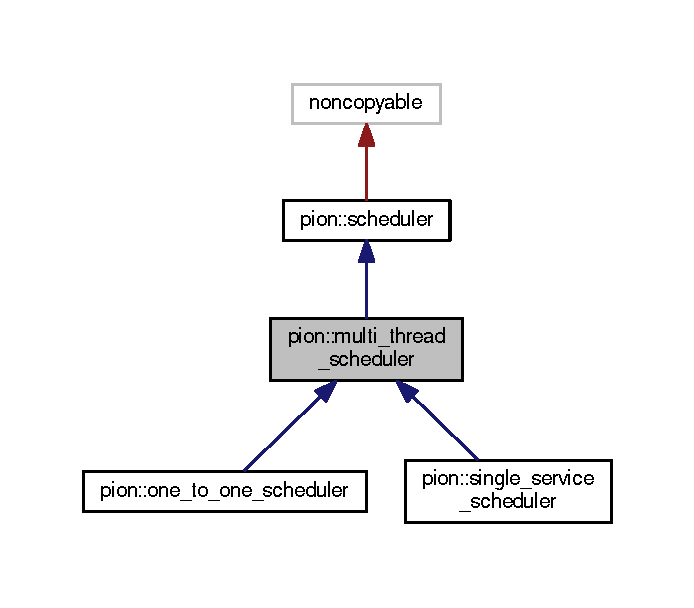
\includegraphics[width=333pt]{classpion_1_1multi__thread__scheduler__inherit__graph}
\end{center}
\end{figure}


Collaboration diagram for pion\-:\-:multi\-\_\-thread\-\_\-scheduler\-:
\nopagebreak
\begin{figure}[H]
\begin{center}
\leavevmode
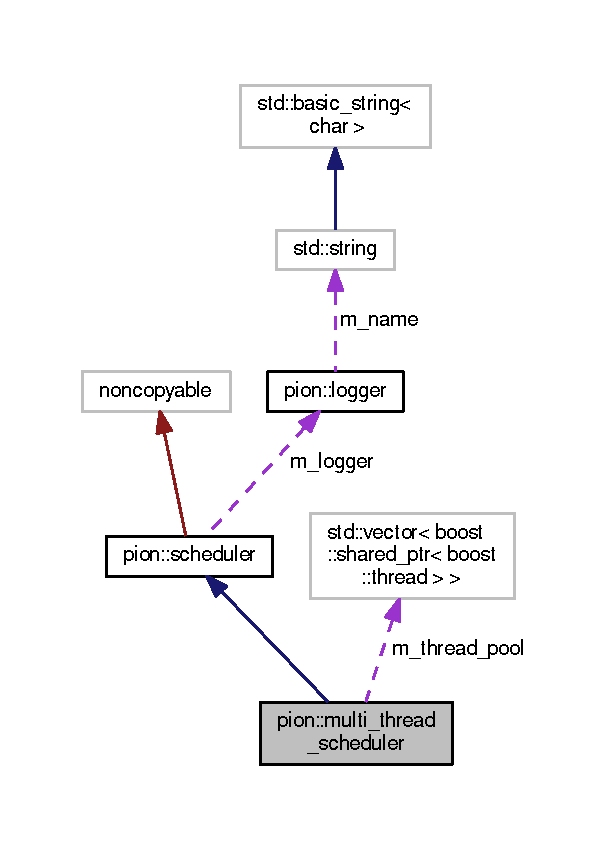
\includegraphics[width=293pt]{classpion_1_1multi__thread__scheduler__coll__graph}
\end{center}
\end{figure}
\subsection*{Public Member Functions}
\begin{DoxyCompactItemize}
\item 
\hyperlink{classpion_1_1multi__thread__scheduler_a7e60ea90622a43533abd1c7c6106d66c}{multi\-\_\-thread\-\_\-scheduler} (void)
\begin{DoxyCompactList}\small\item\em constructs a new \hyperlink{classpion_1_1multi__thread__scheduler}{multi\-\_\-thread\-\_\-scheduler} \end{DoxyCompactList}\item 
virtual \hyperlink{classpion_1_1multi__thread__scheduler_a708525e3a1d80e350ca7030c8859221e}{$\sim$multi\-\_\-thread\-\_\-scheduler} ()
\begin{DoxyCompactList}\small\item\em virtual destructor \end{DoxyCompactList}\end{DoxyCompactItemize}
\subsection*{Protected Types}
\begin{DoxyCompactItemize}
\item 
typedef std\-::vector\\*
$<$ boost\-::shared\-\_\-ptr\\*
$<$ boost\-::thread $>$ $>$ \hyperlink{classpion_1_1multi__thread__scheduler_a0cf5fa4c72b0c1f38043cf9ea61efeef}{Thread\-Pool}
\begin{DoxyCompactList}\small\item\em typedef for a pool of worker threads \end{DoxyCompactList}\end{DoxyCompactItemize}
\subsection*{Protected Member Functions}
\begin{DoxyCompactItemize}
\item 
virtual void \hyperlink{classpion_1_1multi__thread__scheduler_a91945cc6c4a05a716fec36fc48474265}{stop\-\_\-threads} (void)
\begin{DoxyCompactList}\small\item\em stops all threads used to perform work \end{DoxyCompactList}\item 
virtual void \hyperlink{classpion_1_1multi__thread__scheduler_a5e602b3bb9fd7208e7d3325f596e8266}{finish\-\_\-threads} (void)
\begin{DoxyCompactList}\small\item\em finishes all threads used to perform work \end{DoxyCompactList}\end{DoxyCompactItemize}
\subsection*{Protected Attributes}
\begin{DoxyCompactItemize}
\item 
\hyperlink{classpion_1_1multi__thread__scheduler_a0cf5fa4c72b0c1f38043cf9ea61efeef}{Thread\-Pool} \hyperlink{classpion_1_1multi__thread__scheduler_ad2b984248e4b064faae3cc3c7e75d30e}{m\-\_\-thread\-\_\-pool}
\begin{DoxyCompactList}\small\item\em pool of threads used to perform work \end{DoxyCompactList}\end{DoxyCompactItemize}
\subsection*{Additional Inherited Members}


\subsection{Detailed Description}
\hyperlink{classpion_1_1multi__thread__scheduler}{multi\-\_\-thread\-\_\-scheduler}\-: uses a pool of threads to perform work 

\subsection{Member Typedef Documentation}
\hypertarget{classpion_1_1multi__thread__scheduler_a0cf5fa4c72b0c1f38043cf9ea61efeef}{\index{pion\-::multi\-\_\-thread\-\_\-scheduler@{pion\-::multi\-\_\-thread\-\_\-scheduler}!Thread\-Pool@{Thread\-Pool}}
\index{Thread\-Pool@{Thread\-Pool}!pion::multi_thread_scheduler@{pion\-::multi\-\_\-thread\-\_\-scheduler}}
\subsubsection[{Thread\-Pool}]{\setlength{\rightskip}{0pt plus 5cm}typedef std\-::vector$<$boost\-::shared\-\_\-ptr$<$boost\-::thread$>$ $>$ {\bf pion\-::multi\-\_\-thread\-\_\-scheduler\-::\-Thread\-Pool}\hspace{0.3cm}{\ttfamily [protected]}}}\label{classpion_1_1multi__thread__scheduler_a0cf5fa4c72b0c1f38043cf9ea61efeef}


typedef for a pool of worker threads 



\subsection{Constructor \& Destructor Documentation}
\hypertarget{classpion_1_1multi__thread__scheduler_a7e60ea90622a43533abd1c7c6106d66c}{\index{pion\-::multi\-\_\-thread\-\_\-scheduler@{pion\-::multi\-\_\-thread\-\_\-scheduler}!multi\-\_\-thread\-\_\-scheduler@{multi\-\_\-thread\-\_\-scheduler}}
\index{multi\-\_\-thread\-\_\-scheduler@{multi\-\_\-thread\-\_\-scheduler}!pion::multi_thread_scheduler@{pion\-::multi\-\_\-thread\-\_\-scheduler}}
\subsubsection[{multi\-\_\-thread\-\_\-scheduler}]{\setlength{\rightskip}{0pt plus 5cm}pion\-::multi\-\_\-thread\-\_\-scheduler\-::multi\-\_\-thread\-\_\-scheduler (
\begin{DoxyParamCaption}
\item[{void}]{}
\end{DoxyParamCaption}
)\hspace{0.3cm}{\ttfamily [inline]}}}\label{classpion_1_1multi__thread__scheduler_a7e60ea90622a43533abd1c7c6106d66c}


constructs a new \hyperlink{classpion_1_1multi__thread__scheduler}{multi\-\_\-thread\-\_\-scheduler} 

\hypertarget{classpion_1_1multi__thread__scheduler_a708525e3a1d80e350ca7030c8859221e}{\index{pion\-::multi\-\_\-thread\-\_\-scheduler@{pion\-::multi\-\_\-thread\-\_\-scheduler}!$\sim$multi\-\_\-thread\-\_\-scheduler@{$\sim$multi\-\_\-thread\-\_\-scheduler}}
\index{$\sim$multi\-\_\-thread\-\_\-scheduler@{$\sim$multi\-\_\-thread\-\_\-scheduler}!pion::multi_thread_scheduler@{pion\-::multi\-\_\-thread\-\_\-scheduler}}
\subsubsection[{$\sim$multi\-\_\-thread\-\_\-scheduler}]{\setlength{\rightskip}{0pt plus 5cm}virtual pion\-::multi\-\_\-thread\-\_\-scheduler\-::$\sim$multi\-\_\-thread\-\_\-scheduler (
\begin{DoxyParamCaption}
{}
\end{DoxyParamCaption}
)\hspace{0.3cm}{\ttfamily [inline]}, {\ttfamily [virtual]}}}\label{classpion_1_1multi__thread__scheduler_a708525e3a1d80e350ca7030c8859221e}


virtual destructor 



\subsection{Member Function Documentation}
\hypertarget{classpion_1_1multi__thread__scheduler_a5e602b3bb9fd7208e7d3325f596e8266}{\index{pion\-::multi\-\_\-thread\-\_\-scheduler@{pion\-::multi\-\_\-thread\-\_\-scheduler}!finish\-\_\-threads@{finish\-\_\-threads}}
\index{finish\-\_\-threads@{finish\-\_\-threads}!pion::multi_thread_scheduler@{pion\-::multi\-\_\-thread\-\_\-scheduler}}
\subsubsection[{finish\-\_\-threads}]{\setlength{\rightskip}{0pt plus 5cm}virtual void pion\-::multi\-\_\-thread\-\_\-scheduler\-::finish\-\_\-threads (
\begin{DoxyParamCaption}
\item[{void}]{}
\end{DoxyParamCaption}
)\hspace{0.3cm}{\ttfamily [inline]}, {\ttfamily [protected]}, {\ttfamily [virtual]}}}\label{classpion_1_1multi__thread__scheduler_a5e602b3bb9fd7208e7d3325f596e8266}


finishes all threads used to perform work 



Reimplemented from \hyperlink{classpion_1_1scheduler_a6436e075a8c23734e55329f4286b5509}{pion\-::scheduler}.

\hypertarget{classpion_1_1multi__thread__scheduler_a91945cc6c4a05a716fec36fc48474265}{\index{pion\-::multi\-\_\-thread\-\_\-scheduler@{pion\-::multi\-\_\-thread\-\_\-scheduler}!stop\-\_\-threads@{stop\-\_\-threads}}
\index{stop\-\_\-threads@{stop\-\_\-threads}!pion::multi_thread_scheduler@{pion\-::multi\-\_\-thread\-\_\-scheduler}}
\subsubsection[{stop\-\_\-threads}]{\setlength{\rightskip}{0pt plus 5cm}virtual void pion\-::multi\-\_\-thread\-\_\-scheduler\-::stop\-\_\-threads (
\begin{DoxyParamCaption}
\item[{void}]{}
\end{DoxyParamCaption}
)\hspace{0.3cm}{\ttfamily [inline]}, {\ttfamily [protected]}, {\ttfamily [virtual]}}}\label{classpion_1_1multi__thread__scheduler_a91945cc6c4a05a716fec36fc48474265}


stops all threads used to perform work 



Reimplemented from \hyperlink{classpion_1_1scheduler_abd7b1239bb9cf5a6ca1492341adfc4db}{pion\-::scheduler}.



References P\-I\-O\-N\-\_\-\-L\-O\-G\-\_\-\-D\-E\-B\-U\-G.



\subsection{Member Data Documentation}
\hypertarget{classpion_1_1multi__thread__scheduler_ad2b984248e4b064faae3cc3c7e75d30e}{\index{pion\-::multi\-\_\-thread\-\_\-scheduler@{pion\-::multi\-\_\-thread\-\_\-scheduler}!m\-\_\-thread\-\_\-pool@{m\-\_\-thread\-\_\-pool}}
\index{m\-\_\-thread\-\_\-pool@{m\-\_\-thread\-\_\-pool}!pion::multi_thread_scheduler@{pion\-::multi\-\_\-thread\-\_\-scheduler}}
\subsubsection[{m\-\_\-thread\-\_\-pool}]{\setlength{\rightskip}{0pt plus 5cm}{\bf Thread\-Pool} pion\-::multi\-\_\-thread\-\_\-scheduler\-::m\-\_\-thread\-\_\-pool\hspace{0.3cm}{\ttfamily [protected]}}}\label{classpion_1_1multi__thread__scheduler_ad2b984248e4b064faae3cc3c7e75d30e}


pool of threads used to perform work 



Referenced by pion\-::single\-\_\-service\-\_\-scheduler\-::startup(), and pion\-::one\-\_\-to\-\_\-one\-\_\-scheduler\-::startup().



The documentation for this class was generated from the following file\-:\begin{DoxyCompactItemize}
\item 
include/pion/\hyperlink{scheduler_8hpp}{scheduler.\-hpp}\end{DoxyCompactItemize}

\hypertarget{classpion_1_1one__to__one__scheduler}{\section{pion\-:\-:one\-\_\-to\-\_\-one\-\_\-scheduler Class Reference}
\label{classpion_1_1one__to__one__scheduler}\index{pion\-::one\-\_\-to\-\_\-one\-\_\-scheduler@{pion\-::one\-\_\-to\-\_\-one\-\_\-scheduler}}
}


{\ttfamily \#include $<$scheduler.\-hpp$>$}



Inheritance diagram for pion\-:\-:one\-\_\-to\-\_\-one\-\_\-scheduler\-:
\nopagebreak
\begin{figure}[H]
\begin{center}
\leavevmode
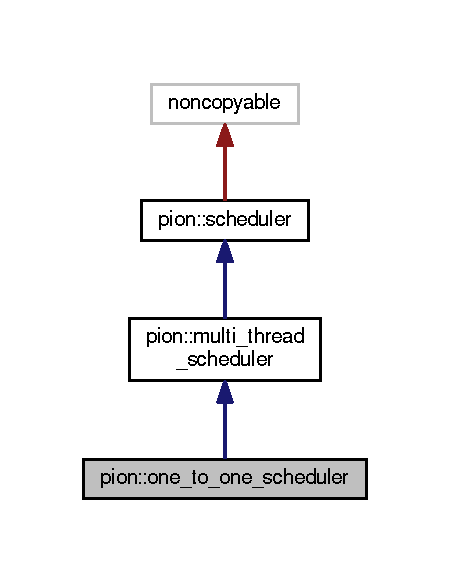
\includegraphics[width=216pt]{classpion_1_1one__to__one__scheduler__inherit__graph}
\end{center}
\end{figure}


Collaboration diagram for pion\-:\-:one\-\_\-to\-\_\-one\-\_\-scheduler\-:
\nopagebreak
\begin{figure}[H]
\begin{center}
\leavevmode
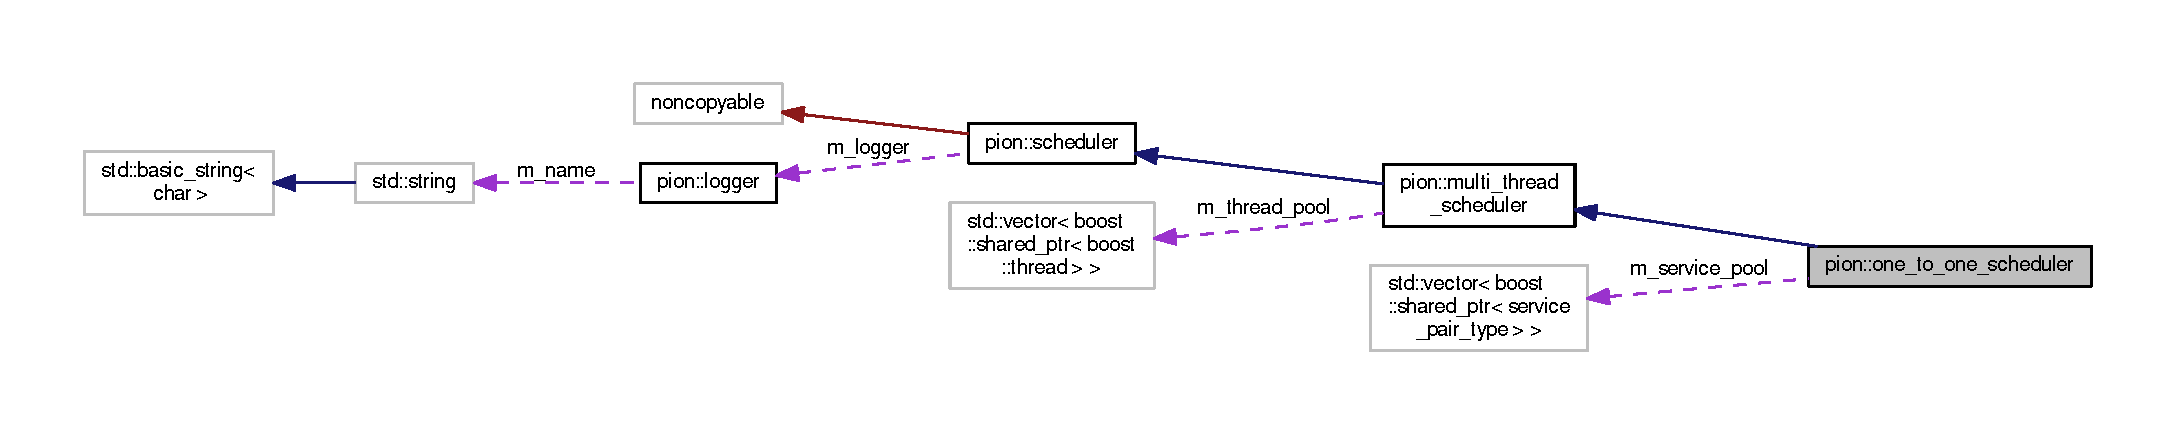
\includegraphics[width=350pt]{classpion_1_1one__to__one__scheduler__coll__graph}
\end{center}
\end{figure}
\subsection*{Classes}
\begin{DoxyCompactItemize}
\item 
struct \hyperlink{structpion_1_1one__to__one__scheduler_1_1service__pair__type}{service\-\_\-pair\-\_\-type}
\begin{DoxyCompactList}\small\item\em typedef for a pair object where first is an I\-O service and second is a deadline timer \end{DoxyCompactList}\end{DoxyCompactItemize}
\subsection*{Public Member Functions}
\begin{DoxyCompactItemize}
\item 
\hyperlink{classpion_1_1one__to__one__scheduler_a1cf085d6cabbbe06891f316a3c0cb938}{one\-\_\-to\-\_\-one\-\_\-scheduler} (void)
\begin{DoxyCompactList}\small\item\em constructs a new \hyperlink{classpion_1_1one__to__one__scheduler}{one\-\_\-to\-\_\-one\-\_\-scheduler} \end{DoxyCompactList}\item 
virtual \hyperlink{classpion_1_1one__to__one__scheduler_a76da28c9f319dced91f30b1d303da518}{$\sim$one\-\_\-to\-\_\-one\-\_\-scheduler} ()
\begin{DoxyCompactList}\small\item\em virtual destructor \end{DoxyCompactList}\item 
virtual boost\-::asio\-::io\-\_\-service \& \hyperlink{classpion_1_1one__to__one__scheduler_a6ead3ddcbbcbfb0eba98b102530d2a90}{get\-\_\-io\-\_\-service} (void)
\begin{DoxyCompactList}\small\item\em returns an async I/\-O service used to schedule work \end{DoxyCompactList}\item 
virtual boost\-::asio\-::io\-\_\-service \& \hyperlink{classpion_1_1one__to__one__scheduler_a5af0e30b2ef08cbbaf40278c9066c166}{get\-\_\-io\-\_\-service} (boost\-::uint32\-\_\-t n)
\item 
virtual void \hyperlink{classpion_1_1one__to__one__scheduler_a8f32fd88bc0d95d9952c5045849e09b9}{startup} (void)
\begin{DoxyCompactList}\small\item\em Starts the thread scheduler (this is called automatically when necessary) \end{DoxyCompactList}\end{DoxyCompactItemize}
\subsection*{Protected Types}
\begin{DoxyCompactItemize}
\item 
typedef std\-::vector\\*
$<$ boost\-::shared\-\_\-ptr\\*
$<$ \hyperlink{structpion_1_1one__to__one__scheduler_1_1service__pair__type}{service\-\_\-pair\-\_\-type} $>$ $>$ \hyperlink{classpion_1_1one__to__one__scheduler_ac41a2d4f38f49673139a77e609b1d084}{service\-\_\-pool\-\_\-type}
\begin{DoxyCompactList}\small\item\em typedef for a pool of I\-O services \end{DoxyCompactList}\end{DoxyCompactItemize}
\subsection*{Protected Member Functions}
\begin{DoxyCompactItemize}
\item 
virtual void \hyperlink{classpion_1_1one__to__one__scheduler_a39c02d4a67bf5cd28da3ce22363dd698}{stop\-\_\-services} (void)
\begin{DoxyCompactList}\small\item\em stops all services used to schedule work \end{DoxyCompactList}\item 
virtual void \hyperlink{classpion_1_1one__to__one__scheduler_a3e9f1380789598587a27f0857e7c9133}{finish\-\_\-services} (void)
\begin{DoxyCompactList}\small\item\em finishes all services used to schedule work \end{DoxyCompactList}\end{DoxyCompactItemize}
\subsection*{Protected Attributes}
\begin{DoxyCompactItemize}
\item 
\hyperlink{classpion_1_1one__to__one__scheduler_ac41a2d4f38f49673139a77e609b1d084}{service\-\_\-pool\-\_\-type} \hyperlink{classpion_1_1one__to__one__scheduler_a8b6ae075086a579e46ca08a89085c07a}{m\-\_\-service\-\_\-pool}
\begin{DoxyCompactList}\small\item\em pool of I\-O services used to schedule work \end{DoxyCompactList}\item 
boost\-::uint32\-\_\-t \hyperlink{classpion_1_1one__to__one__scheduler_ae4e2b2a157c1c9e36694e86b6ae354b1}{m\-\_\-next\-\_\-service}
\begin{DoxyCompactList}\small\item\em the next service to use for scheduling work \end{DoxyCompactList}\end{DoxyCompactItemize}
\subsection*{Additional Inherited Members}


\subsection{Detailed Description}
\hyperlink{classpion_1_1one__to__one__scheduler}{one\-\_\-to\-\_\-one\-\_\-scheduler}\-: uses a single I\-O service for each thread 

\subsection{Member Typedef Documentation}
\hypertarget{classpion_1_1one__to__one__scheduler_ac41a2d4f38f49673139a77e609b1d084}{\index{pion\-::one\-\_\-to\-\_\-one\-\_\-scheduler@{pion\-::one\-\_\-to\-\_\-one\-\_\-scheduler}!service\-\_\-pool\-\_\-type@{service\-\_\-pool\-\_\-type}}
\index{service\-\_\-pool\-\_\-type@{service\-\_\-pool\-\_\-type}!pion::one_to_one_scheduler@{pion\-::one\-\_\-to\-\_\-one\-\_\-scheduler}}
\subsubsection[{service\-\_\-pool\-\_\-type}]{\setlength{\rightskip}{0pt plus 5cm}typedef std\-::vector$<$boost\-::shared\-\_\-ptr$<${\bf service\-\_\-pair\-\_\-type}$>$ $>$ {\bf pion\-::one\-\_\-to\-\_\-one\-\_\-scheduler\-::service\-\_\-pool\-\_\-type}\hspace{0.3cm}{\ttfamily [protected]}}}\label{classpion_1_1one__to__one__scheduler_ac41a2d4f38f49673139a77e609b1d084}


typedef for a pool of I\-O services 



\subsection{Constructor \& Destructor Documentation}
\hypertarget{classpion_1_1one__to__one__scheduler_a1cf085d6cabbbe06891f316a3c0cb938}{\index{pion\-::one\-\_\-to\-\_\-one\-\_\-scheduler@{pion\-::one\-\_\-to\-\_\-one\-\_\-scheduler}!one\-\_\-to\-\_\-one\-\_\-scheduler@{one\-\_\-to\-\_\-one\-\_\-scheduler}}
\index{one\-\_\-to\-\_\-one\-\_\-scheduler@{one\-\_\-to\-\_\-one\-\_\-scheduler}!pion::one_to_one_scheduler@{pion\-::one\-\_\-to\-\_\-one\-\_\-scheduler}}
\subsubsection[{one\-\_\-to\-\_\-one\-\_\-scheduler}]{\setlength{\rightskip}{0pt plus 5cm}pion\-::one\-\_\-to\-\_\-one\-\_\-scheduler\-::one\-\_\-to\-\_\-one\-\_\-scheduler (
\begin{DoxyParamCaption}
\item[{void}]{}
\end{DoxyParamCaption}
)\hspace{0.3cm}{\ttfamily [inline]}}}\label{classpion_1_1one__to__one__scheduler_a1cf085d6cabbbe06891f316a3c0cb938}


constructs a new \hyperlink{classpion_1_1one__to__one__scheduler}{one\-\_\-to\-\_\-one\-\_\-scheduler} 

\hypertarget{classpion_1_1one__to__one__scheduler_a76da28c9f319dced91f30b1d303da518}{\index{pion\-::one\-\_\-to\-\_\-one\-\_\-scheduler@{pion\-::one\-\_\-to\-\_\-one\-\_\-scheduler}!$\sim$one\-\_\-to\-\_\-one\-\_\-scheduler@{$\sim$one\-\_\-to\-\_\-one\-\_\-scheduler}}
\index{$\sim$one\-\_\-to\-\_\-one\-\_\-scheduler@{$\sim$one\-\_\-to\-\_\-one\-\_\-scheduler}!pion::one_to_one_scheduler@{pion\-::one\-\_\-to\-\_\-one\-\_\-scheduler}}
\subsubsection[{$\sim$one\-\_\-to\-\_\-one\-\_\-scheduler}]{\setlength{\rightskip}{0pt plus 5cm}virtual pion\-::one\-\_\-to\-\_\-one\-\_\-scheduler\-::$\sim$one\-\_\-to\-\_\-one\-\_\-scheduler (
\begin{DoxyParamCaption}
{}
\end{DoxyParamCaption}
)\hspace{0.3cm}{\ttfamily [inline]}, {\ttfamily [virtual]}}}\label{classpion_1_1one__to__one__scheduler_a76da28c9f319dced91f30b1d303da518}


virtual destructor 



\subsection{Member Function Documentation}
\hypertarget{classpion_1_1one__to__one__scheduler_a3e9f1380789598587a27f0857e7c9133}{\index{pion\-::one\-\_\-to\-\_\-one\-\_\-scheduler@{pion\-::one\-\_\-to\-\_\-one\-\_\-scheduler}!finish\-\_\-services@{finish\-\_\-services}}
\index{finish\-\_\-services@{finish\-\_\-services}!pion::one_to_one_scheduler@{pion\-::one\-\_\-to\-\_\-one\-\_\-scheduler}}
\subsubsection[{finish\-\_\-services}]{\setlength{\rightskip}{0pt plus 5cm}virtual void pion\-::one\-\_\-to\-\_\-one\-\_\-scheduler\-::finish\-\_\-services (
\begin{DoxyParamCaption}
\item[{void}]{}
\end{DoxyParamCaption}
)\hspace{0.3cm}{\ttfamily [inline]}, {\ttfamily [protected]}, {\ttfamily [virtual]}}}\label{classpion_1_1one__to__one__scheduler_a3e9f1380789598587a27f0857e7c9133}


finishes all services used to schedule work 



Reimplemented from \hyperlink{classpion_1_1scheduler_a64dbc267db8e1481f80ba6d42bbb24ea}{pion\-::scheduler}.

\hypertarget{classpion_1_1one__to__one__scheduler_a6ead3ddcbbcbfb0eba98b102530d2a90}{\index{pion\-::one\-\_\-to\-\_\-one\-\_\-scheduler@{pion\-::one\-\_\-to\-\_\-one\-\_\-scheduler}!get\-\_\-io\-\_\-service@{get\-\_\-io\-\_\-service}}
\index{get\-\_\-io\-\_\-service@{get\-\_\-io\-\_\-service}!pion::one_to_one_scheduler@{pion\-::one\-\_\-to\-\_\-one\-\_\-scheduler}}
\subsubsection[{get\-\_\-io\-\_\-service}]{\setlength{\rightskip}{0pt plus 5cm}virtual boost\-::asio\-::io\-\_\-service\& pion\-::one\-\_\-to\-\_\-one\-\_\-scheduler\-::get\-\_\-io\-\_\-service (
\begin{DoxyParamCaption}
\item[{void}]{}
\end{DoxyParamCaption}
)\hspace{0.3cm}{\ttfamily [inline]}, {\ttfamily [virtual]}}}\label{classpion_1_1one__to__one__scheduler_a6ead3ddcbbcbfb0eba98b102530d2a90}


returns an async I/\-O service used to schedule work 



Implements \hyperlink{classpion_1_1scheduler_a037e0ee2c2c83b7002180a4656ccbbfa}{pion\-::scheduler}.

\hypertarget{classpion_1_1one__to__one__scheduler_a5af0e30b2ef08cbbaf40278c9066c166}{\index{pion\-::one\-\_\-to\-\_\-one\-\_\-scheduler@{pion\-::one\-\_\-to\-\_\-one\-\_\-scheduler}!get\-\_\-io\-\_\-service@{get\-\_\-io\-\_\-service}}
\index{get\-\_\-io\-\_\-service@{get\-\_\-io\-\_\-service}!pion::one_to_one_scheduler@{pion\-::one\-\_\-to\-\_\-one\-\_\-scheduler}}
\subsubsection[{get\-\_\-io\-\_\-service}]{\setlength{\rightskip}{0pt plus 5cm}virtual boost\-::asio\-::io\-\_\-service\& pion\-::one\-\_\-to\-\_\-one\-\_\-scheduler\-::get\-\_\-io\-\_\-service (
\begin{DoxyParamCaption}
\item[{boost\-::uint32\-\_\-t}]{n}
\end{DoxyParamCaption}
)\hspace{0.3cm}{\ttfamily [inline]}, {\ttfamily [virtual]}}}\label{classpion_1_1one__to__one__scheduler_a5af0e30b2ef08cbbaf40278c9066c166}
returns an async I/\-O service used to schedule work (provides direct access to avoid locking when possible)


\begin{DoxyParams}{Parameters}
{\em n} & integer number representing the service object \\
\hline
\end{DoxyParams}
\hypertarget{classpion_1_1one__to__one__scheduler_a8f32fd88bc0d95d9952c5045849e09b9}{\index{pion\-::one\-\_\-to\-\_\-one\-\_\-scheduler@{pion\-::one\-\_\-to\-\_\-one\-\_\-scheduler}!startup@{startup}}
\index{startup@{startup}!pion::one_to_one_scheduler@{pion\-::one\-\_\-to\-\_\-one\-\_\-scheduler}}
\subsubsection[{startup}]{\setlength{\rightskip}{0pt plus 5cm}void pion\-::one\-\_\-to\-\_\-one\-\_\-scheduler\-::startup (
\begin{DoxyParamCaption}
\item[{void}]{}
\end{DoxyParamCaption}
)\hspace{0.3cm}{\ttfamily [virtual]}}}\label{classpion_1_1one__to__one__scheduler_a8f32fd88bc0d95d9952c5045849e09b9}


Starts the thread scheduler (this is called automatically when necessary) 



Reimplemented from \hyperlink{classpion_1_1scheduler_ab656139dc844a547d5c1001b3ef17d13}{pion\-::scheduler}.



References pion\-::scheduler\-::keep\-\_\-running(), pion\-::scheduler\-::m\-\_\-is\-\_\-running, pion\-::scheduler\-::m\-\_\-logger, pion\-::scheduler\-::m\-\_\-mutex, pion\-::scheduler\-::m\-\_\-num\-\_\-threads, m\-\_\-service\-\_\-pool, pion\-::multi\-\_\-thread\-\_\-scheduler\-::m\-\_\-thread\-\_\-pool, P\-I\-O\-N\-\_\-\-L\-O\-G\-\_\-\-I\-N\-F\-O, and pion\-::scheduler\-::process\-\_\-service\-\_\-work().

\hypertarget{classpion_1_1one__to__one__scheduler_a39c02d4a67bf5cd28da3ce22363dd698}{\index{pion\-::one\-\_\-to\-\_\-one\-\_\-scheduler@{pion\-::one\-\_\-to\-\_\-one\-\_\-scheduler}!stop\-\_\-services@{stop\-\_\-services}}
\index{stop\-\_\-services@{stop\-\_\-services}!pion::one_to_one_scheduler@{pion\-::one\-\_\-to\-\_\-one\-\_\-scheduler}}
\subsubsection[{stop\-\_\-services}]{\setlength{\rightskip}{0pt plus 5cm}virtual void pion\-::one\-\_\-to\-\_\-one\-\_\-scheduler\-::stop\-\_\-services (
\begin{DoxyParamCaption}
\item[{void}]{}
\end{DoxyParamCaption}
)\hspace{0.3cm}{\ttfamily [inline]}, {\ttfamily [protected]}, {\ttfamily [virtual]}}}\label{classpion_1_1one__to__one__scheduler_a39c02d4a67bf5cd28da3ce22363dd698}


stops all services used to schedule work 



Reimplemented from \hyperlink{classpion_1_1scheduler_a62b59f0561bd527d78768fd3a5ceeb36}{pion\-::scheduler}.



\subsection{Member Data Documentation}
\hypertarget{classpion_1_1one__to__one__scheduler_ae4e2b2a157c1c9e36694e86b6ae354b1}{\index{pion\-::one\-\_\-to\-\_\-one\-\_\-scheduler@{pion\-::one\-\_\-to\-\_\-one\-\_\-scheduler}!m\-\_\-next\-\_\-service@{m\-\_\-next\-\_\-service}}
\index{m\-\_\-next\-\_\-service@{m\-\_\-next\-\_\-service}!pion::one_to_one_scheduler@{pion\-::one\-\_\-to\-\_\-one\-\_\-scheduler}}
\subsubsection[{m\-\_\-next\-\_\-service}]{\setlength{\rightskip}{0pt plus 5cm}boost\-::uint32\-\_\-t pion\-::one\-\_\-to\-\_\-one\-\_\-scheduler\-::m\-\_\-next\-\_\-service\hspace{0.3cm}{\ttfamily [protected]}}}\label{classpion_1_1one__to__one__scheduler_ae4e2b2a157c1c9e36694e86b6ae354b1}


the next service to use for scheduling work 

\hypertarget{classpion_1_1one__to__one__scheduler_a8b6ae075086a579e46ca08a89085c07a}{\index{pion\-::one\-\_\-to\-\_\-one\-\_\-scheduler@{pion\-::one\-\_\-to\-\_\-one\-\_\-scheduler}!m\-\_\-service\-\_\-pool@{m\-\_\-service\-\_\-pool}}
\index{m\-\_\-service\-\_\-pool@{m\-\_\-service\-\_\-pool}!pion::one_to_one_scheduler@{pion\-::one\-\_\-to\-\_\-one\-\_\-scheduler}}
\subsubsection[{m\-\_\-service\-\_\-pool}]{\setlength{\rightskip}{0pt plus 5cm}{\bf service\-\_\-pool\-\_\-type} pion\-::one\-\_\-to\-\_\-one\-\_\-scheduler\-::m\-\_\-service\-\_\-pool\hspace{0.3cm}{\ttfamily [protected]}}}\label{classpion_1_1one__to__one__scheduler_a8b6ae075086a579e46ca08a89085c07a}


pool of I\-O services used to schedule work 



Referenced by startup().



The documentation for this class was generated from the following files\-:\begin{DoxyCompactItemize}
\item 
include/pion/\hyperlink{scheduler_8hpp}{scheduler.\-hpp}\item 
src/\hyperlink{scheduler_8cpp}{scheduler.\-cpp}\end{DoxyCompactItemize}

\hypertarget{classpion_1_1error_1_1open__file}{\section{pion\-:\-:error\-:\-:open\-\_\-file Class Reference}
\label{classpion_1_1error_1_1open__file}\index{pion\-::error\-::open\-\_\-file@{pion\-::error\-::open\-\_\-file}}
}


exception thrown if we failed to open a file  




{\ttfamily \#include $<$error.\-hpp$>$}



Inheritance diagram for pion\-:\-:error\-:\-:open\-\_\-file\-:
\nopagebreak
\begin{figure}[H]
\begin{center}
\leavevmode
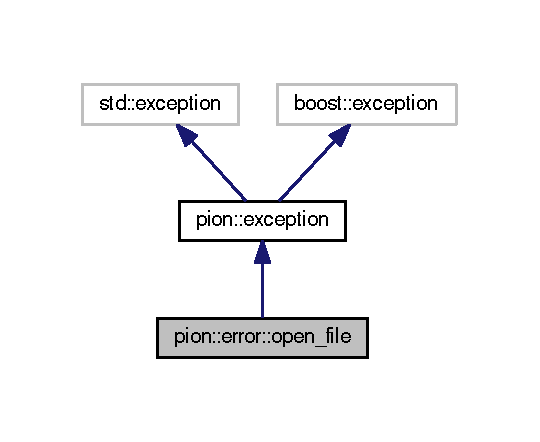
\includegraphics[width=259pt]{classpion_1_1error_1_1open__file__inherit__graph}
\end{center}
\end{figure}


Collaboration diagram for pion\-:\-:error\-:\-:open\-\_\-file\-:
\nopagebreak
\begin{figure}[H]
\begin{center}
\leavevmode
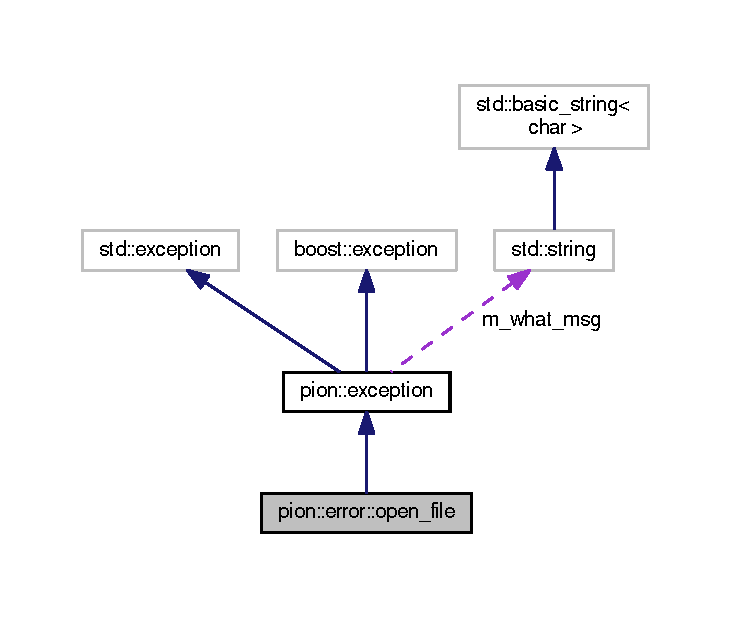
\includegraphics[width=350pt]{classpion_1_1error_1_1open__file__coll__graph}
\end{center}
\end{figure}
\subsection*{Additional Inherited Members}


\subsection{Detailed Description}
exception thrown if we failed to open a file 

The documentation for this class was generated from the following file\-:\begin{DoxyCompactItemize}
\item 
include/pion/\hyperlink{error_8hpp}{error.\-hpp}\end{DoxyCompactItemize}

\hypertarget{classpion_1_1error_1_1open__plugin}{\section{pion\-:\-:error\-:\-:open\-\_\-plugin Class Reference}
\label{classpion_1_1error_1_1open__plugin}\index{pion\-::error\-::open\-\_\-plugin@{pion\-::error\-::open\-\_\-plugin}}
}


exception thrown if we are unable to open a plugin  




{\ttfamily \#include $<$error.\-hpp$>$}



Inheritance diagram for pion\-:\-:error\-:\-:open\-\_\-plugin\-:
\nopagebreak
\begin{figure}[H]
\begin{center}
\leavevmode
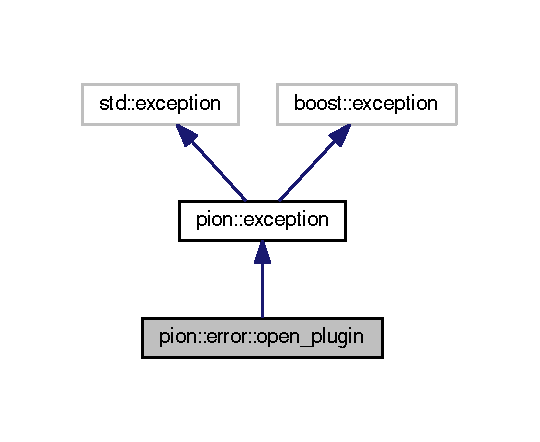
\includegraphics[width=259pt]{classpion_1_1error_1_1open__plugin__inherit__graph}
\end{center}
\end{figure}


Collaboration diagram for pion\-:\-:error\-:\-:open\-\_\-plugin\-:
\nopagebreak
\begin{figure}[H]
\begin{center}
\leavevmode
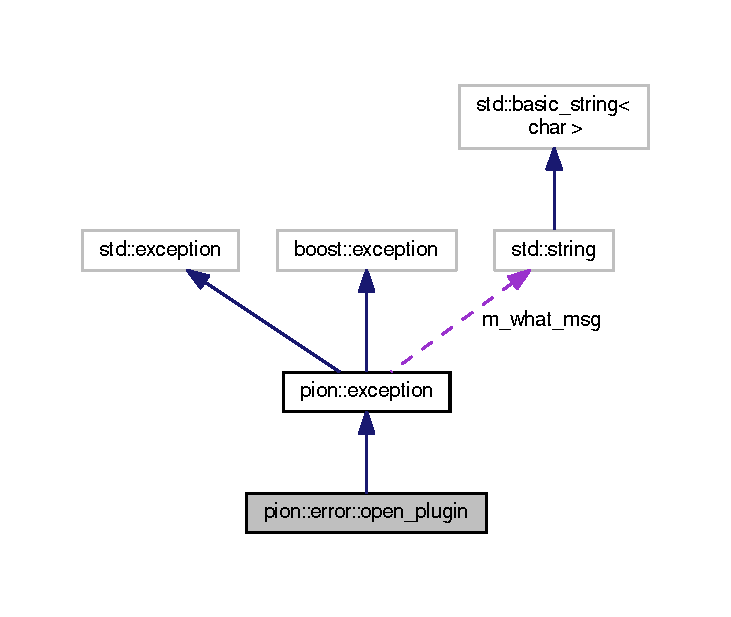
\includegraphics[width=350pt]{classpion_1_1error_1_1open__plugin__coll__graph}
\end{center}
\end{figure}
\subsection*{Additional Inherited Members}


\subsection{Detailed Description}
exception thrown if we are unable to open a plugin 

The documentation for this class was generated from the following file\-:\begin{DoxyCompactItemize}
\item 
include/pion/\hyperlink{error_8hpp}{error.\-hpp}\end{DoxyCompactItemize}

\hypertarget{classpion_1_1http_1_1parser}{\section{pion\-:\-:http\-:\-:parser Class Reference}
\label{classpion_1_1http_1_1parser}\index{pion\-::http\-::parser@{pion\-::http\-::parser}}
}


{\ttfamily \#include $<$parser.\-hpp$>$}



Inheritance diagram for pion\-:\-:http\-:\-:parser\-:
\nopagebreak
\begin{figure}[H]
\begin{center}
\leavevmode
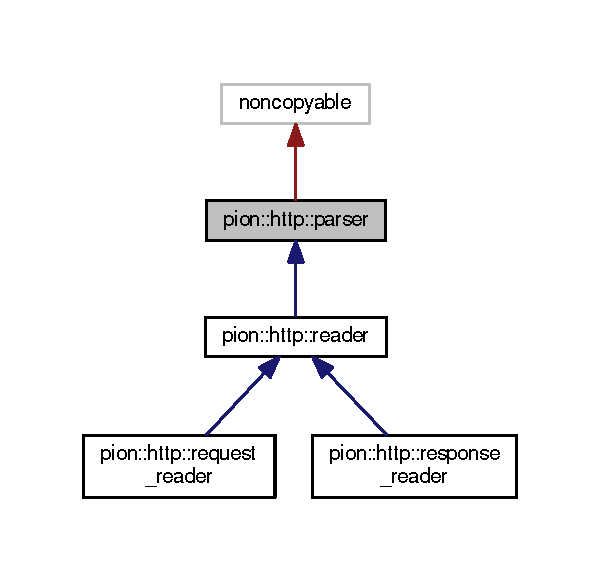
\includegraphics[width=288pt]{classpion_1_1http_1_1parser__inherit__graph}
\end{center}
\end{figure}


Collaboration diagram for pion\-:\-:http\-:\-:parser\-:
\nopagebreak
\begin{figure}[H]
\begin{center}
\leavevmode
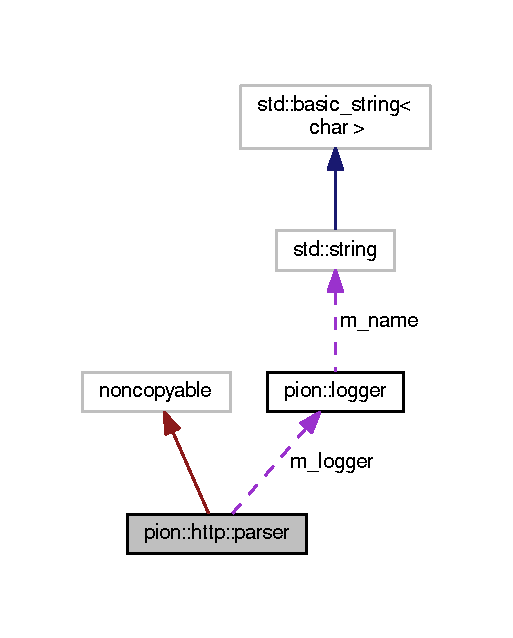
\includegraphics[width=246pt]{classpion_1_1http_1_1parser__coll__graph}
\end{center}
\end{figure}
\subsection*{Classes}
\begin{DoxyCompactItemize}
\item 
class \hyperlink{classpion_1_1http_1_1parser_1_1error__category__t}{error\-\_\-category\-\_\-t}
\begin{DoxyCompactList}\small\item\em class-\/specific error category \end{DoxyCompactList}\end{DoxyCompactItemize}
\subsection*{Public Types}
\begin{DoxyCompactItemize}
\item 
enum \hyperlink{classpion_1_1http_1_1parser_a056c791c4b2dda0dd4c2037dd941d5d8}{error\-\_\-value\-\_\-t} \{ \\*
\hyperlink{classpion_1_1http_1_1parser_a056c791c4b2dda0dd4c2037dd941d5d8a0cc5469207de11a5179956d3d17a8ab1}{E\-R\-R\-O\-R\-\_\-\-M\-E\-T\-H\-O\-D\-\_\-\-C\-H\-A\-R} = 1, 
\hyperlink{classpion_1_1http_1_1parser_a056c791c4b2dda0dd4c2037dd941d5d8a1462b9df44708776a05f5601f42846a8}{E\-R\-R\-O\-R\-\_\-\-M\-E\-T\-H\-O\-D\-\_\-\-S\-I\-Z\-E}, 
\hyperlink{classpion_1_1http_1_1parser_a056c791c4b2dda0dd4c2037dd941d5d8a54942737d9dda2528f9061cabc407fe9}{E\-R\-R\-O\-R\-\_\-\-U\-R\-I\-\_\-\-C\-H\-A\-R}, 
\hyperlink{classpion_1_1http_1_1parser_a056c791c4b2dda0dd4c2037dd941d5d8ab567f2418ac85f479280135441a5a390}{E\-R\-R\-O\-R\-\_\-\-U\-R\-I\-\_\-\-S\-I\-Z\-E}, 
\\*
\hyperlink{classpion_1_1http_1_1parser_a056c791c4b2dda0dd4c2037dd941d5d8a4f9ae6c0f7de1da68c85795429afda14}{E\-R\-R\-O\-R\-\_\-\-Q\-U\-E\-R\-Y\-\_\-\-C\-H\-A\-R}, 
\hyperlink{classpion_1_1http_1_1parser_a056c791c4b2dda0dd4c2037dd941d5d8aad97a47e56d77fc8d7e46a587e70e0ed}{E\-R\-R\-O\-R\-\_\-\-Q\-U\-E\-R\-Y\-\_\-\-S\-I\-Z\-E}, 
\hyperlink{classpion_1_1http_1_1parser_a056c791c4b2dda0dd4c2037dd941d5d8a35a28be377bf93eba3edaa51b0ab6a9c}{E\-R\-R\-O\-R\-\_\-\-V\-E\-R\-S\-I\-O\-N\-\_\-\-E\-M\-P\-T\-Y}, 
\hyperlink{classpion_1_1http_1_1parser_a056c791c4b2dda0dd4c2037dd941d5d8a640437b0cc21cccc547a3f838d9bdd10}{E\-R\-R\-O\-R\-\_\-\-V\-E\-R\-S\-I\-O\-N\-\_\-\-C\-H\-A\-R}, 
\\*
\hyperlink{classpion_1_1http_1_1parser_a056c791c4b2dda0dd4c2037dd941d5d8a0ee250337cb43c76158f6094f6f273fc}{E\-R\-R\-O\-R\-\_\-\-S\-T\-A\-T\-U\-S\-\_\-\-E\-M\-P\-T\-Y}, 
\hyperlink{classpion_1_1http_1_1parser_a056c791c4b2dda0dd4c2037dd941d5d8a1df2c04224d1c647c08e7249bc666317}{E\-R\-R\-O\-R\-\_\-\-S\-T\-A\-T\-U\-S\-\_\-\-C\-H\-A\-R}, 
\hyperlink{classpion_1_1http_1_1parser_a056c791c4b2dda0dd4c2037dd941d5d8ae695d24cfd40b5354d5d3def0c7bbefd}{E\-R\-R\-O\-R\-\_\-\-H\-E\-A\-D\-E\-R\-\_\-\-C\-H\-A\-R}, 
\hyperlink{classpion_1_1http_1_1parser_a056c791c4b2dda0dd4c2037dd941d5d8a968de881fea53ccb84f3dc98c380ef53}{E\-R\-R\-O\-R\-\_\-\-H\-E\-A\-D\-E\-R\-\_\-\-N\-A\-M\-E\-\_\-\-S\-I\-Z\-E}, 
\\*
\hyperlink{classpion_1_1http_1_1parser_a056c791c4b2dda0dd4c2037dd941d5d8aa713c03b93494671a51a2097cbb9d1b9}{E\-R\-R\-O\-R\-\_\-\-H\-E\-A\-D\-E\-R\-\_\-\-V\-A\-L\-U\-E\-\_\-\-S\-I\-Z\-E}, 
\hyperlink{classpion_1_1http_1_1parser_a056c791c4b2dda0dd4c2037dd941d5d8af042c54007443f7919571b2cf6f52d70}{E\-R\-R\-O\-R\-\_\-\-I\-N\-V\-A\-L\-I\-D\-\_\-\-C\-O\-N\-T\-E\-N\-T\-\_\-\-L\-E\-N\-G\-T\-H}, 
\hyperlink{classpion_1_1http_1_1parser_a056c791c4b2dda0dd4c2037dd941d5d8abfd2136b613537506493c193b5e8caf1}{E\-R\-R\-O\-R\-\_\-\-C\-H\-U\-N\-K\-\_\-\-C\-H\-A\-R}, 
\hyperlink{classpion_1_1http_1_1parser_a056c791c4b2dda0dd4c2037dd941d5d8ade97f557fc11c10a56c93caa07ff5df2}{E\-R\-R\-O\-R\-\_\-\-M\-I\-S\-S\-I\-N\-G\-\_\-\-C\-H\-U\-N\-K\-\_\-\-D\-A\-T\-A}, 
\\*
\hyperlink{classpion_1_1http_1_1parser_a056c791c4b2dda0dd4c2037dd941d5d8ad3c9d5e280da006c16899b1c8a58c8fe}{E\-R\-R\-O\-R\-\_\-\-M\-I\-S\-S\-I\-N\-G\-\_\-\-H\-E\-A\-D\-E\-R\-\_\-\-D\-A\-T\-A}, 
\hyperlink{classpion_1_1http_1_1parser_a056c791c4b2dda0dd4c2037dd941d5d8aa652e202a02ae20a5fefe8d222d7df67}{E\-R\-R\-O\-R\-\_\-\-M\-I\-S\-S\-I\-N\-G\-\_\-\-T\-O\-O\-\_\-\-M\-U\-C\-H\-\_\-\-C\-O\-N\-T\-E\-N\-T}
 \}
\begin{DoxyCompactList}\small\item\em class-\/specific error code values \end{DoxyCompactList}\item 
typedef boost\-::function2$<$ void, \\*
const char $\ast$, std\-::size\-\_\-t $>$ \hyperlink{classpion_1_1http_1_1parser_abff772b79d2a912b0f9a4932d8f03a35}{payload\-\_\-handler\-\_\-t}
\begin{DoxyCompactList}\small\item\em callback type used to consume payload content \end{DoxyCompactList}\end{DoxyCompactItemize}
\subsection*{Public Member Functions}
\begin{DoxyCompactItemize}
\item 
\hyperlink{classpion_1_1http_1_1parser_a33fe9cfd9bcae8868b817332d38a9261}{parser} (const bool is\-\_\-request, std\-::size\-\_\-t max\-\_\-content\-\_\-length=\hyperlink{classpion_1_1http_1_1parser_a77d2e93061f62e1b7028c783145adf22}{D\-E\-F\-A\-U\-L\-T\-\_\-\-C\-O\-N\-T\-E\-N\-T\-\_\-\-M\-A\-X})
\item 
virtual \hyperlink{classpion_1_1http_1_1parser_ac9df3da159b11389dba00e222410a599}{$\sim$parser} ()
\begin{DoxyCompactList}\small\item\em default destructor \end{DoxyCompactList}\item 
boost\-::tribool \hyperlink{classpion_1_1http_1_1parser_aead5bbb8da80c78bc2de3c264e4ace9c}{parse} (\hyperlink{classpion_1_1http_1_1message}{http\-::message} \&http\-\_\-msg, boost\-::system\-::error\-\_\-code \&ec)
\item 
boost\-::tribool \hyperlink{classpion_1_1http_1_1parser_ae77669284c876d7b107ba30a78af6d02}{parse\-\_\-missing\-\_\-data} (\hyperlink{classpion_1_1http_1_1message}{http\-::message} \&http\-\_\-msg, std\-::size\-\_\-t len, boost\-::system\-::error\-\_\-code \&ec)
\item 
void \hyperlink{classpion_1_1http_1_1parser_afcf9b52d540f78af9177642a5c571362}{finish} (\hyperlink{classpion_1_1http_1_1message}{http\-::message} \&http\-\_\-msg) const 
\item 
void \hyperlink{classpion_1_1http_1_1parser_a71fdd1e6e681a3bd932baf2bd6a9f9c9}{set\-\_\-read\-\_\-buffer} (const char $\ast$ptr, size\-\_\-t len)
\item 
void \hyperlink{classpion_1_1http_1_1parser_a3feba34ee7fb1c4f59dda5c1e58d3d82}{load\-\_\-read\-\_\-pos} (const char $\ast$\&read\-\_\-ptr, const char $\ast$\&read\-\_\-end\-\_\-ptr) const 
\item 
bool \hyperlink{classpion_1_1http_1_1parser_ad41eedba2dd5977ffddb1bc65dddc8fc}{check\-\_\-premature\-\_\-eof} (\hyperlink{classpion_1_1http_1_1message}{http\-::message} \&http\-\_\-msg)
\item 
void \hyperlink{classpion_1_1http_1_1parser_a1f7f084f396c9c912d65426883b33a38}{parse\-\_\-headers\-\_\-only} (bool b=true)
\item 
void \hyperlink{classpion_1_1http_1_1parser_a0fb8ebee189b4c3613ee67c85e2ac9ce}{skip\-\_\-header\-\_\-parsing} (\hyperlink{classpion_1_1http_1_1message}{http\-::message} \&http\-\_\-msg)
\item 
void \hyperlink{classpion_1_1http_1_1parser_aed8cfd92c078205e38294bd8109eb2d3}{reset} (void)
\begin{DoxyCompactList}\small\item\em resets the parser to its initial state \end{DoxyCompactList}\item 
bool \hyperlink{classpion_1_1http_1_1parser_adf957476284a4833ea89306e412b1862}{eof} (void) const 
\begin{DoxyCompactList}\small\item\em returns true if there are no more bytes available in the read buffer \end{DoxyCompactList}\item 
std\-::size\-\_\-t \hyperlink{classpion_1_1http_1_1parser_a4e8f394a1c2296ac01d2c16c5128b7b4}{bytes\-\_\-available} (void) const 
\begin{DoxyCompactList}\small\item\em returns the number of bytes available in the read buffer \end{DoxyCompactList}\item 
std\-::size\-\_\-t \hyperlink{classpion_1_1http_1_1parser_ad708d537fabbc3093ea0ea9a519567dc}{gcount} (void) const 
\begin{DoxyCompactList}\small\item\em returns the number of bytes read during the last parse operation \end{DoxyCompactList}\item 
std\-::size\-\_\-t \hyperlink{classpion_1_1http_1_1parser_ae458700259bab34f090832c3bc23ab80}{get\-\_\-total\-\_\-bytes\-\_\-read} (void) const 
\begin{DoxyCompactList}\small\item\em returns the total number of bytes read while parsing the H\-T\-T\-P message \end{DoxyCompactList}\item 
std\-::size\-\_\-t \hyperlink{classpion_1_1http_1_1parser_ab0ca19c444c2d3cf816347422b1c5402}{get\-\_\-content\-\_\-bytes\-\_\-read} (void) const 
\begin{DoxyCompactList}\small\item\em returns the total number of bytes read while parsing the payload content \end{DoxyCompactList}\item 
std\-::size\-\_\-t \hyperlink{classpion_1_1http_1_1parser_a2c6bf6775a9b1d8f1965190ef0dec780}{get\-\_\-max\-\_\-content\-\_\-length} (void) const 
\begin{DoxyCompactList}\small\item\em returns the maximum length for H\-T\-T\-P payload content \end{DoxyCompactList}\item 
const std\-::string \& \hyperlink{classpion_1_1http_1_1parser_a83774cd75b3a549a72ad45da17c99431}{get\-\_\-raw\-\_\-headers} (void) const 
\begin{DoxyCompactList}\small\item\em returns the raw H\-T\-T\-P headers saved by the parser \end{DoxyCompactList}\item 
bool \hyperlink{classpion_1_1http_1_1parser_ab5b4e9b0acdd3cd6b4ac3cfcc76c9a6f}{get\-\_\-save\-\_\-raw\-\_\-headers} (void) const 
\begin{DoxyCompactList}\small\item\em returns true if the parser is saving raw H\-T\-T\-P header contents \end{DoxyCompactList}\item 
bool \hyperlink{classpion_1_1http_1_1parser_a37e691fd12abb6be3bf2f0dda3c412d7}{get\-\_\-parse\-\_\-headers\-\_\-only} (void)
\begin{DoxyCompactList}\small\item\em returns true if parsing headers only \end{DoxyCompactList}\item 
bool \hyperlink{classpion_1_1http_1_1parser_a94bf8701f781109b664d10e86bd67b8f}{is\-\_\-parsing\-\_\-request} (void) const 
\begin{DoxyCompactList}\small\item\em returns true if the parser is being used to parse an H\-T\-T\-P request \end{DoxyCompactList}\item 
bool \hyperlink{classpion_1_1http_1_1parser_a057f0ee607bef1057902093f12861c1f}{is\-\_\-parsing\-\_\-response} (void) const 
\begin{DoxyCompactList}\small\item\em returns true if the parser is being used to parse an H\-T\-T\-P response \end{DoxyCompactList}\item 
void \hyperlink{classpion_1_1http_1_1parser_a4605c605bf452336f34d7d48fce68ef6}{set\-\_\-payload\-\_\-handler} (\hyperlink{classpion_1_1http_1_1parser_abff772b79d2a912b0f9a4932d8f03a35}{payload\-\_\-handler\-\_\-t} \&h)
\begin{DoxyCompactList}\small\item\em defines a callback function to be used for consuming payload content \end{DoxyCompactList}\item 
void \hyperlink{classpion_1_1http_1_1parser_a6533144b6f6d1e93dd000360748ac271}{set\-\_\-max\-\_\-content\-\_\-length} (std\-::size\-\_\-t n)
\begin{DoxyCompactList}\small\item\em sets the maximum length for H\-T\-T\-P payload content \end{DoxyCompactList}\item 
void \hyperlink{classpion_1_1http_1_1parser_a8834a77e417b4127bdda4fa79ff5fe59}{reset\-\_\-max\-\_\-content\-\_\-length} (void)
\begin{DoxyCompactList}\small\item\em resets the maximum length for H\-T\-T\-P payload content to the default value \end{DoxyCompactList}\item 
void \hyperlink{classpion_1_1http_1_1parser_a06b96d27daaea9ae3dd15f188e01f70b}{set\-\_\-save\-\_\-raw\-\_\-headers} (bool b)
\begin{DoxyCompactList}\small\item\em sets parameter for saving raw H\-T\-T\-P header content \end{DoxyCompactList}\item 
void \hyperlink{classpion_1_1http_1_1parser_a3f93047d2f938a845967d22073122311}{set\-\_\-logger} (\hyperlink{structpion_1_1logger}{logger} log\-\_\-ptr)
\begin{DoxyCompactList}\small\item\em sets the logger to be used \end{DoxyCompactList}\item 
\hyperlink{structpion_1_1logger}{logger} \hyperlink{classpion_1_1http_1_1parser_ad799af46a7b4e3f1e27c047f76849d77}{get\-\_\-logger} (void)
\begin{DoxyCompactList}\small\item\em returns the logger currently in use \end{DoxyCompactList}\item 
boost\-::tribool \hyperlink{classpion_1_1http_1_1parser_ac707ec5cecacf3b56c151e6891c5cf9d}{finish\-\_\-header\-\_\-parsing} (\hyperlink{classpion_1_1http_1_1message}{http\-::message} \&http\-\_\-msg, boost\-::system\-::error\-\_\-code \&ec)
\end{DoxyCompactItemize}
\subsection*{Static Public Member Functions}
\begin{DoxyCompactItemize}
\item 
static bool \hyperlink{classpion_1_1http_1_1parser_a0688e577644445e854e6e9c1d614fd25}{parse\-\_\-uri} (const std\-::string \&uri, std\-::string \&proto, std\-::string \&host, boost\-::uint16\-\_\-t \&port, std\-::string \&path, std\-::string \&query)
\item 
static bool \hyperlink{classpion_1_1http_1_1parser_a3cda26a67405acd5ba04ee19bca52ea7}{parse\-\_\-url\-\_\-encoded} (\hyperlink{namespacepion_a2cd31d7bbe0e98008bd4e6f135103c0e}{ihash\-\_\-multimap} \&dict, const char $\ast$ptr, const std\-::size\-\_\-t len)
\item 
static bool \hyperlink{classpion_1_1http_1_1parser_aa297a0f51bb5a605fb99f188066d9e15}{parse\-\_\-multipart\-\_\-form\-\_\-data} (\hyperlink{namespacepion_a2cd31d7bbe0e98008bd4e6f135103c0e}{ihash\-\_\-multimap} \&dict, const std\-::string \&content\-\_\-type, const char $\ast$ptr, const std\-::size\-\_\-t len)
\item 
static bool \hyperlink{classpion_1_1http_1_1parser_af9a9744b9376e79d4cc05d8c37533bec}{parse\-\_\-cookie\-\_\-header} (\hyperlink{namespacepion_a2cd31d7bbe0e98008bd4e6f135103c0e}{ihash\-\_\-multimap} \&dict, const char $\ast$ptr, const std\-::size\-\_\-t len, bool set\-\_\-cookie\-\_\-header)
\item 
static bool \hyperlink{classpion_1_1http_1_1parser_aaf57ebb2c31ecb126d5c4b2aba305417}{parse\-\_\-cookie\-\_\-header} (\hyperlink{namespacepion_a2cd31d7bbe0e98008bd4e6f135103c0e}{ihash\-\_\-multimap} \&dict, const std\-::string \&cookie\-\_\-header, bool set\-\_\-cookie\-\_\-header)
\item 
static bool \hyperlink{classpion_1_1http_1_1parser_a988623311585ce6097c90586f5711ee0}{parse\-\_\-url\-\_\-encoded} (\hyperlink{namespacepion_a2cd31d7bbe0e98008bd4e6f135103c0e}{ihash\-\_\-multimap} \&dict, const std\-::string \&query)
\item 
static bool \hyperlink{classpion_1_1http_1_1parser_a456501e5a0e9b83fb3c030b003b60676}{parse\-\_\-multipart\-\_\-form\-\_\-data} (\hyperlink{namespacepion_a2cd31d7bbe0e98008bd4e6f135103c0e}{ihash\-\_\-multimap} \&dict, const std\-::string \&content\-\_\-type, const std\-::string \&form\-\_\-data)
\item 
static bool \hyperlink{classpion_1_1http_1_1parser_ab8bd069a0ae8fb51fb8ec6c3d02c065b}{parse\-\_\-forwarded\-\_\-for} (const std\-::string \&header, std\-::string \&public\-\_\-ip)
\item 
static \hyperlink{classpion_1_1http_1_1parser_1_1error__category__t}{error\-\_\-category\-\_\-t} \& \hyperlink{classpion_1_1http_1_1parser_a9313aa230ae4af4c30702c0605a1f701}{get\-\_\-error\-\_\-category} (void)
\begin{DoxyCompactList}\small\item\em returns an instance of \hyperlink{classpion_1_1http_1_1parser_1_1error__category__t}{parser\-::error\-\_\-category\-\_\-t} \end{DoxyCompactList}\end{DoxyCompactItemize}
\subsection*{Static Public Attributes}
\begin{DoxyCompactItemize}
\item 
static const std\-::size\-\_\-t \hyperlink{classpion_1_1http_1_1parser_a77d2e93061f62e1b7028c783145adf22}{D\-E\-F\-A\-U\-L\-T\-\_\-\-C\-O\-N\-T\-E\-N\-T\-\_\-\-M\-A\-X} = 1024 $\ast$ 1024
\begin{DoxyCompactList}\small\item\em maximum length for H\-T\-T\-P payload content \end{DoxyCompactList}\end{DoxyCompactItemize}
\subsection*{Protected Member Functions}
\begin{DoxyCompactItemize}
\item 
virtual void \hyperlink{classpion_1_1http_1_1parser_abed3c66097728d826c4ec771837803ea}{finished\-\_\-parsing\-\_\-headers} (const boost\-::system\-::error\-\_\-code \&)
\begin{DoxyCompactList}\small\item\em Called after we have finished parsing the H\-T\-T\-P message headers. \end{DoxyCompactList}\item 
boost\-::tribool \hyperlink{classpion_1_1http_1_1parser_a7377c221aaf546cfaf98fdb308c8739e}{parse\-\_\-headers} (\hyperlink{classpion_1_1http_1_1message}{http\-::message} \&http\-\_\-msg, boost\-::system\-::error\-\_\-code \&ec)
\item 
void \hyperlink{classpion_1_1http_1_1parser_ad1ffb1db7870fa7cfbcfe743a67aca23}{update\-\_\-message\-\_\-with\-\_\-header\-\_\-data} (\hyperlink{classpion_1_1http_1_1message}{http\-::message} \&http\-\_\-msg) const 
\item 
boost\-::tribool \hyperlink{classpion_1_1http_1_1parser_a658f65ec298a48e01054490da841f75c}{parse\-\_\-chunks} (\hyperlink{classpion_1_1http_1_1message_a4bcf1ea1d4e7a5637d04ae109adb5e46}{http\-::message\-::chunk\-\_\-cache\-\_\-t} \&chunk\-\_\-buffers, boost\-::system\-::error\-\_\-code \&ec)
\item 
boost\-::tribool \hyperlink{classpion_1_1http_1_1parser_aaff1b32ea824c7d7782f8e58346506a7}{consume\-\_\-content} (\hyperlink{classpion_1_1http_1_1message}{http\-::message} \&http\-\_\-msg, boost\-::system\-::error\-\_\-code \&ec)
\item 
std\-::size\-\_\-t \hyperlink{classpion_1_1http_1_1parser_ac7234e092bdd29379a23b720e6566f56}{consume\-\_\-content\-\_\-as\-\_\-next\-\_\-chunk} (\hyperlink{classpion_1_1http_1_1message_a4bcf1ea1d4e7a5637d04ae109adb5e46}{http\-::message\-::chunk\-\_\-cache\-\_\-t} \&chunk\-\_\-buffers)
\end{DoxyCompactItemize}
\subsection*{Static Protected Member Functions}
\begin{DoxyCompactItemize}
\item 
static void \hyperlink{classpion_1_1http_1_1parser_a50628b4ffc6ab8f0cf46873d6e8075bb}{compute\-\_\-msg\-\_\-status} (\hyperlink{classpion_1_1http_1_1message}{http\-::message} \&http\-\_\-msg, bool msg\-\_\-parsed\-\_\-ok)
\item 
static void \hyperlink{classpion_1_1http_1_1parser_a0d8875ea346743ed37ae0cd7c2a73672}{set\-\_\-error} (boost\-::system\-::error\-\_\-code \&ec, \hyperlink{classpion_1_1http_1_1parser_a056c791c4b2dda0dd4c2037dd941d5d8}{error\-\_\-value\-\_\-t} ev)
\item 
static void \hyperlink{classpion_1_1http_1_1parser_ad16455747863108b62c77d89bd5dcf0d}{create\-\_\-error\-\_\-category} (void)
\begin{DoxyCompactList}\small\item\em creates the unique parser \hyperlink{classpion_1_1http_1_1parser_1_1error__category__t}{error\-\_\-category\-\_\-t} \end{DoxyCompactList}\item 
static bool \hyperlink{classpion_1_1http_1_1parser_aa1099c00a26a33a615dfd54fd945873c}{is\-\_\-char} (int c)
\item 
static bool \hyperlink{classpion_1_1http_1_1parser_aaf665f61057ffc430746134b88f20d11}{is\-\_\-control} (int c)
\item 
static bool \hyperlink{classpion_1_1http_1_1parser_a0e5e96ae29b09b95e407eb63403fa2a3}{is\-\_\-special} (int c)
\item 
static bool \hyperlink{classpion_1_1http_1_1parser_add90b4c4bb8cc44eb79d2e6ba989ae9a}{is\-\_\-digit} (int c)
\item 
static bool \hyperlink{classpion_1_1http_1_1parser_a3d83fdf4309c2b57284759948b2bbc4b}{is\-\_\-hex\-\_\-digit} (int c)
\item 
static bool \hyperlink{classpion_1_1http_1_1parser_abeb585af8111e5a5f99d1ce87f6e107b}{is\-\_\-cookie\-\_\-attribute} (const std\-::string \&name, bool set\-\_\-cookie\-\_\-header)
\end{DoxyCompactItemize}
\subsection*{Protected Attributes}
\begin{DoxyCompactItemize}
\item 
\hyperlink{structpion_1_1logger}{logger} \hyperlink{classpion_1_1http_1_1parser_ac0df021ba559d1af96dc9b0a5fa99df5}{m\-\_\-logger}
\begin{DoxyCompactList}\small\item\em primary logging interface used by this class \end{DoxyCompactList}\item 
const bool \hyperlink{classpion_1_1http_1_1parser_a5c24acf28ddd9c6133be4aa3127da530}{m\-\_\-is\-\_\-request}
\begin{DoxyCompactList}\small\item\em true if the message is an H\-T\-T\-P request; false if it is an H\-T\-T\-P response \end{DoxyCompactList}\item 
const char $\ast$ \hyperlink{classpion_1_1http_1_1parser_a3ca52095a690cb92197755a5eea24cd7}{m\-\_\-read\-\_\-ptr}
\begin{DoxyCompactList}\small\item\em points to the next character to be consumed in the read\-\_\-buffer \end{DoxyCompactList}\item 
const char $\ast$ \hyperlink{classpion_1_1http_1_1parser_a6788da854f2d77ae2c92c739d0a2c191}{m\-\_\-read\-\_\-end\-\_\-ptr}
\begin{DoxyCompactList}\small\item\em points to the end of the read\-\_\-buffer (last byte + 1) \end{DoxyCompactList}\end{DoxyCompactItemize}
\subsection*{Static Protected Attributes}
\begin{DoxyCompactItemize}
\item 
static const boost\-::uint32\-\_\-t \hyperlink{classpion_1_1http_1_1parser_a5480070912368dd015d72d54fcbece66}{S\-T\-A\-T\-U\-S\-\_\-\-M\-E\-S\-S\-A\-G\-E\-\_\-\-M\-A\-X} = 1024
\begin{DoxyCompactList}\small\item\em maximum length for response status message \end{DoxyCompactList}\item 
static const boost\-::uint32\-\_\-t \hyperlink{classpion_1_1http_1_1parser_ad781cc2dcdb333a8d286a4534d4509cb}{M\-E\-T\-H\-O\-D\-\_\-\-M\-A\-X} = 1024
\begin{DoxyCompactList}\small\item\em maximum length for the request method \end{DoxyCompactList}\item 
static const boost\-::uint32\-\_\-t \hyperlink{classpion_1_1http_1_1parser_adf1d822b13731ee6430d5cfd8ad78a95}{R\-E\-S\-O\-U\-R\-C\-E\-\_\-\-M\-A\-X} = 256 $\ast$ 1024
\begin{DoxyCompactList}\small\item\em maximum length for the resource requested \end{DoxyCompactList}\item 
static const boost\-::uint32\-\_\-t \hyperlink{classpion_1_1http_1_1parser_a2ef9e2d01055c727c40cd6af47cbfd2a}{Q\-U\-E\-R\-Y\-\_\-\-S\-T\-R\-I\-N\-G\-\_\-\-M\-A\-X} = 1024 $\ast$ 1024
\begin{DoxyCompactList}\small\item\em maximum length for the query string \end{DoxyCompactList}\item 
static const boost\-::uint32\-\_\-t \hyperlink{classpion_1_1http_1_1parser_aa0d75346e6643078bb48efe9c382497d}{H\-E\-A\-D\-E\-R\-\_\-\-N\-A\-M\-E\-\_\-\-M\-A\-X} = 1024
\begin{DoxyCompactList}\small\item\em maximum length for an H\-T\-T\-P header name \end{DoxyCompactList}\item 
static const boost\-::uint32\-\_\-t \hyperlink{classpion_1_1http_1_1parser_a803490d20fadf6ee1253dd9d62844dd8}{H\-E\-A\-D\-E\-R\-\_\-\-V\-A\-L\-U\-E\-\_\-\-M\-A\-X} = 1024 $\ast$ 1024
\begin{DoxyCompactList}\small\item\em maximum length for an H\-T\-T\-P header value \end{DoxyCompactList}\item 
static const boost\-::uint32\-\_\-t \hyperlink{classpion_1_1http_1_1parser_a730afd8438cd3c179bafc7d9eaad27b6}{Q\-U\-E\-R\-Y\-\_\-\-N\-A\-M\-E\-\_\-\-M\-A\-X} = 1024
\begin{DoxyCompactList}\small\item\em maximum length for the name of a query string variable \end{DoxyCompactList}\item 
static const boost\-::uint32\-\_\-t \hyperlink{classpion_1_1http_1_1parser_a5b0039834377ba6797d6628acf59f240}{Q\-U\-E\-R\-Y\-\_\-\-V\-A\-L\-U\-E\-\_\-\-M\-A\-X} = 1024 $\ast$ 1024
\begin{DoxyCompactList}\small\item\em maximum length for the value of a query string variable \end{DoxyCompactList}\item 
static const boost\-::uint32\-\_\-t \hyperlink{classpion_1_1http_1_1parser_a12cb4b88d7debd8467cc9de786721be2}{C\-O\-O\-K\-I\-E\-\_\-\-N\-A\-M\-E\-\_\-\-M\-A\-X} = 1024
\begin{DoxyCompactList}\small\item\em maximum length for the name of a cookie name \end{DoxyCompactList}\item 
static const boost\-::uint32\-\_\-t \hyperlink{classpion_1_1http_1_1parser_a50ae5c379ee3ad611fa6874bfcd8ed83}{C\-O\-O\-K\-I\-E\-\_\-\-V\-A\-L\-U\-E\-\_\-\-M\-A\-X} = 1024 $\ast$ 1024
\begin{DoxyCompactList}\small\item\em maximum length for the value of a cookie; also used for path and domain \end{DoxyCompactList}\end{DoxyCompactItemize}


\subsection{Detailed Description}
parser\-: parses H\-T\-T\-P messages 

\subsection{Member Typedef Documentation}
\hypertarget{classpion_1_1http_1_1parser_abff772b79d2a912b0f9a4932d8f03a35}{\index{pion\-::http\-::parser@{pion\-::http\-::parser}!payload\-\_\-handler\-\_\-t@{payload\-\_\-handler\-\_\-t}}
\index{payload\-\_\-handler\-\_\-t@{payload\-\_\-handler\-\_\-t}!pion::http::parser@{pion\-::http\-::parser}}
\subsubsection[{payload\-\_\-handler\-\_\-t}]{\setlength{\rightskip}{0pt plus 5cm}typedef boost\-::function2$<$void, const char $\ast$, std\-::size\-\_\-t$>$ {\bf pion\-::http\-::parser\-::payload\-\_\-handler\-\_\-t}}}\label{classpion_1_1http_1_1parser_abff772b79d2a912b0f9a4932d8f03a35}


callback type used to consume payload content 



\subsection{Member Enumeration Documentation}
\hypertarget{classpion_1_1http_1_1parser_a056c791c4b2dda0dd4c2037dd941d5d8}{\index{pion\-::http\-::parser@{pion\-::http\-::parser}!error\-\_\-value\-\_\-t@{error\-\_\-value\-\_\-t}}
\index{error\-\_\-value\-\_\-t@{error\-\_\-value\-\_\-t}!pion::http::parser@{pion\-::http\-::parser}}
\subsubsection[{error\-\_\-value\-\_\-t}]{\setlength{\rightskip}{0pt plus 5cm}enum {\bf pion\-::http\-::parser\-::error\-\_\-value\-\_\-t}}}\label{classpion_1_1http_1_1parser_a056c791c4b2dda0dd4c2037dd941d5d8}


class-\/specific error code values 

\begin{Desc}
\item[Enumerator]\par
\begin{description}
\index{E\-R\-R\-O\-R\-\_\-\-M\-E\-T\-H\-O\-D\-\_\-\-C\-H\-A\-R@{E\-R\-R\-O\-R\-\_\-\-M\-E\-T\-H\-O\-D\-\_\-\-C\-H\-A\-R}!pion\-::http\-::parser@{pion\-::http\-::parser}}\index{pion\-::http\-::parser@{pion\-::http\-::parser}!E\-R\-R\-O\-R\-\_\-\-M\-E\-T\-H\-O\-D\-\_\-\-C\-H\-A\-R@{E\-R\-R\-O\-R\-\_\-\-M\-E\-T\-H\-O\-D\-\_\-\-C\-H\-A\-R}}\item[{\em 
\hypertarget{classpion_1_1http_1_1parser_a056c791c4b2dda0dd4c2037dd941d5d8a0cc5469207de11a5179956d3d17a8ab1}{E\-R\-R\-O\-R\-\_\-\-M\-E\-T\-H\-O\-D\-\_\-\-C\-H\-A\-R}\label{classpion_1_1http_1_1parser_a056c791c4b2dda0dd4c2037dd941d5d8a0cc5469207de11a5179956d3d17a8ab1}
}]\index{E\-R\-R\-O\-R\-\_\-\-M\-E\-T\-H\-O\-D\-\_\-\-S\-I\-Z\-E@{E\-R\-R\-O\-R\-\_\-\-M\-E\-T\-H\-O\-D\-\_\-\-S\-I\-Z\-E}!pion\-::http\-::parser@{pion\-::http\-::parser}}\index{pion\-::http\-::parser@{pion\-::http\-::parser}!E\-R\-R\-O\-R\-\_\-\-M\-E\-T\-H\-O\-D\-\_\-\-S\-I\-Z\-E@{E\-R\-R\-O\-R\-\_\-\-M\-E\-T\-H\-O\-D\-\_\-\-S\-I\-Z\-E}}\item[{\em 
\hypertarget{classpion_1_1http_1_1parser_a056c791c4b2dda0dd4c2037dd941d5d8a1462b9df44708776a05f5601f42846a8}{E\-R\-R\-O\-R\-\_\-\-M\-E\-T\-H\-O\-D\-\_\-\-S\-I\-Z\-E}\label{classpion_1_1http_1_1parser_a056c791c4b2dda0dd4c2037dd941d5d8a1462b9df44708776a05f5601f42846a8}
}]\index{E\-R\-R\-O\-R\-\_\-\-U\-R\-I\-\_\-\-C\-H\-A\-R@{E\-R\-R\-O\-R\-\_\-\-U\-R\-I\-\_\-\-C\-H\-A\-R}!pion\-::http\-::parser@{pion\-::http\-::parser}}\index{pion\-::http\-::parser@{pion\-::http\-::parser}!E\-R\-R\-O\-R\-\_\-\-U\-R\-I\-\_\-\-C\-H\-A\-R@{E\-R\-R\-O\-R\-\_\-\-U\-R\-I\-\_\-\-C\-H\-A\-R}}\item[{\em 
\hypertarget{classpion_1_1http_1_1parser_a056c791c4b2dda0dd4c2037dd941d5d8a54942737d9dda2528f9061cabc407fe9}{E\-R\-R\-O\-R\-\_\-\-U\-R\-I\-\_\-\-C\-H\-A\-R}\label{classpion_1_1http_1_1parser_a056c791c4b2dda0dd4c2037dd941d5d8a54942737d9dda2528f9061cabc407fe9}
}]\index{E\-R\-R\-O\-R\-\_\-\-U\-R\-I\-\_\-\-S\-I\-Z\-E@{E\-R\-R\-O\-R\-\_\-\-U\-R\-I\-\_\-\-S\-I\-Z\-E}!pion\-::http\-::parser@{pion\-::http\-::parser}}\index{pion\-::http\-::parser@{pion\-::http\-::parser}!E\-R\-R\-O\-R\-\_\-\-U\-R\-I\-\_\-\-S\-I\-Z\-E@{E\-R\-R\-O\-R\-\_\-\-U\-R\-I\-\_\-\-S\-I\-Z\-E}}\item[{\em 
\hypertarget{classpion_1_1http_1_1parser_a056c791c4b2dda0dd4c2037dd941d5d8ab567f2418ac85f479280135441a5a390}{E\-R\-R\-O\-R\-\_\-\-U\-R\-I\-\_\-\-S\-I\-Z\-E}\label{classpion_1_1http_1_1parser_a056c791c4b2dda0dd4c2037dd941d5d8ab567f2418ac85f479280135441a5a390}
}]\index{E\-R\-R\-O\-R\-\_\-\-Q\-U\-E\-R\-Y\-\_\-\-C\-H\-A\-R@{E\-R\-R\-O\-R\-\_\-\-Q\-U\-E\-R\-Y\-\_\-\-C\-H\-A\-R}!pion\-::http\-::parser@{pion\-::http\-::parser}}\index{pion\-::http\-::parser@{pion\-::http\-::parser}!E\-R\-R\-O\-R\-\_\-\-Q\-U\-E\-R\-Y\-\_\-\-C\-H\-A\-R@{E\-R\-R\-O\-R\-\_\-\-Q\-U\-E\-R\-Y\-\_\-\-C\-H\-A\-R}}\item[{\em 
\hypertarget{classpion_1_1http_1_1parser_a056c791c4b2dda0dd4c2037dd941d5d8a4f9ae6c0f7de1da68c85795429afda14}{E\-R\-R\-O\-R\-\_\-\-Q\-U\-E\-R\-Y\-\_\-\-C\-H\-A\-R}\label{classpion_1_1http_1_1parser_a056c791c4b2dda0dd4c2037dd941d5d8a4f9ae6c0f7de1da68c85795429afda14}
}]\index{E\-R\-R\-O\-R\-\_\-\-Q\-U\-E\-R\-Y\-\_\-\-S\-I\-Z\-E@{E\-R\-R\-O\-R\-\_\-\-Q\-U\-E\-R\-Y\-\_\-\-S\-I\-Z\-E}!pion\-::http\-::parser@{pion\-::http\-::parser}}\index{pion\-::http\-::parser@{pion\-::http\-::parser}!E\-R\-R\-O\-R\-\_\-\-Q\-U\-E\-R\-Y\-\_\-\-S\-I\-Z\-E@{E\-R\-R\-O\-R\-\_\-\-Q\-U\-E\-R\-Y\-\_\-\-S\-I\-Z\-E}}\item[{\em 
\hypertarget{classpion_1_1http_1_1parser_a056c791c4b2dda0dd4c2037dd941d5d8aad97a47e56d77fc8d7e46a587e70e0ed}{E\-R\-R\-O\-R\-\_\-\-Q\-U\-E\-R\-Y\-\_\-\-S\-I\-Z\-E}\label{classpion_1_1http_1_1parser_a056c791c4b2dda0dd4c2037dd941d5d8aad97a47e56d77fc8d7e46a587e70e0ed}
}]\index{E\-R\-R\-O\-R\-\_\-\-V\-E\-R\-S\-I\-O\-N\-\_\-\-E\-M\-P\-T\-Y@{E\-R\-R\-O\-R\-\_\-\-V\-E\-R\-S\-I\-O\-N\-\_\-\-E\-M\-P\-T\-Y}!pion\-::http\-::parser@{pion\-::http\-::parser}}\index{pion\-::http\-::parser@{pion\-::http\-::parser}!E\-R\-R\-O\-R\-\_\-\-V\-E\-R\-S\-I\-O\-N\-\_\-\-E\-M\-P\-T\-Y@{E\-R\-R\-O\-R\-\_\-\-V\-E\-R\-S\-I\-O\-N\-\_\-\-E\-M\-P\-T\-Y}}\item[{\em 
\hypertarget{classpion_1_1http_1_1parser_a056c791c4b2dda0dd4c2037dd941d5d8a35a28be377bf93eba3edaa51b0ab6a9c}{E\-R\-R\-O\-R\-\_\-\-V\-E\-R\-S\-I\-O\-N\-\_\-\-E\-M\-P\-T\-Y}\label{classpion_1_1http_1_1parser_a056c791c4b2dda0dd4c2037dd941d5d8a35a28be377bf93eba3edaa51b0ab6a9c}
}]\index{E\-R\-R\-O\-R\-\_\-\-V\-E\-R\-S\-I\-O\-N\-\_\-\-C\-H\-A\-R@{E\-R\-R\-O\-R\-\_\-\-V\-E\-R\-S\-I\-O\-N\-\_\-\-C\-H\-A\-R}!pion\-::http\-::parser@{pion\-::http\-::parser}}\index{pion\-::http\-::parser@{pion\-::http\-::parser}!E\-R\-R\-O\-R\-\_\-\-V\-E\-R\-S\-I\-O\-N\-\_\-\-C\-H\-A\-R@{E\-R\-R\-O\-R\-\_\-\-V\-E\-R\-S\-I\-O\-N\-\_\-\-C\-H\-A\-R}}\item[{\em 
\hypertarget{classpion_1_1http_1_1parser_a056c791c4b2dda0dd4c2037dd941d5d8a640437b0cc21cccc547a3f838d9bdd10}{E\-R\-R\-O\-R\-\_\-\-V\-E\-R\-S\-I\-O\-N\-\_\-\-C\-H\-A\-R}\label{classpion_1_1http_1_1parser_a056c791c4b2dda0dd4c2037dd941d5d8a640437b0cc21cccc547a3f838d9bdd10}
}]\index{E\-R\-R\-O\-R\-\_\-\-S\-T\-A\-T\-U\-S\-\_\-\-E\-M\-P\-T\-Y@{E\-R\-R\-O\-R\-\_\-\-S\-T\-A\-T\-U\-S\-\_\-\-E\-M\-P\-T\-Y}!pion\-::http\-::parser@{pion\-::http\-::parser}}\index{pion\-::http\-::parser@{pion\-::http\-::parser}!E\-R\-R\-O\-R\-\_\-\-S\-T\-A\-T\-U\-S\-\_\-\-E\-M\-P\-T\-Y@{E\-R\-R\-O\-R\-\_\-\-S\-T\-A\-T\-U\-S\-\_\-\-E\-M\-P\-T\-Y}}\item[{\em 
\hypertarget{classpion_1_1http_1_1parser_a056c791c4b2dda0dd4c2037dd941d5d8a0ee250337cb43c76158f6094f6f273fc}{E\-R\-R\-O\-R\-\_\-\-S\-T\-A\-T\-U\-S\-\_\-\-E\-M\-P\-T\-Y}\label{classpion_1_1http_1_1parser_a056c791c4b2dda0dd4c2037dd941d5d8a0ee250337cb43c76158f6094f6f273fc}
}]\index{E\-R\-R\-O\-R\-\_\-\-S\-T\-A\-T\-U\-S\-\_\-\-C\-H\-A\-R@{E\-R\-R\-O\-R\-\_\-\-S\-T\-A\-T\-U\-S\-\_\-\-C\-H\-A\-R}!pion\-::http\-::parser@{pion\-::http\-::parser}}\index{pion\-::http\-::parser@{pion\-::http\-::parser}!E\-R\-R\-O\-R\-\_\-\-S\-T\-A\-T\-U\-S\-\_\-\-C\-H\-A\-R@{E\-R\-R\-O\-R\-\_\-\-S\-T\-A\-T\-U\-S\-\_\-\-C\-H\-A\-R}}\item[{\em 
\hypertarget{classpion_1_1http_1_1parser_a056c791c4b2dda0dd4c2037dd941d5d8a1df2c04224d1c647c08e7249bc666317}{E\-R\-R\-O\-R\-\_\-\-S\-T\-A\-T\-U\-S\-\_\-\-C\-H\-A\-R}\label{classpion_1_1http_1_1parser_a056c791c4b2dda0dd4c2037dd941d5d8a1df2c04224d1c647c08e7249bc666317}
}]\index{E\-R\-R\-O\-R\-\_\-\-H\-E\-A\-D\-E\-R\-\_\-\-C\-H\-A\-R@{E\-R\-R\-O\-R\-\_\-\-H\-E\-A\-D\-E\-R\-\_\-\-C\-H\-A\-R}!pion\-::http\-::parser@{pion\-::http\-::parser}}\index{pion\-::http\-::parser@{pion\-::http\-::parser}!E\-R\-R\-O\-R\-\_\-\-H\-E\-A\-D\-E\-R\-\_\-\-C\-H\-A\-R@{E\-R\-R\-O\-R\-\_\-\-H\-E\-A\-D\-E\-R\-\_\-\-C\-H\-A\-R}}\item[{\em 
\hypertarget{classpion_1_1http_1_1parser_a056c791c4b2dda0dd4c2037dd941d5d8ae695d24cfd40b5354d5d3def0c7bbefd}{E\-R\-R\-O\-R\-\_\-\-H\-E\-A\-D\-E\-R\-\_\-\-C\-H\-A\-R}\label{classpion_1_1http_1_1parser_a056c791c4b2dda0dd4c2037dd941d5d8ae695d24cfd40b5354d5d3def0c7bbefd}
}]\index{E\-R\-R\-O\-R\-\_\-\-H\-E\-A\-D\-E\-R\-\_\-\-N\-A\-M\-E\-\_\-\-S\-I\-Z\-E@{E\-R\-R\-O\-R\-\_\-\-H\-E\-A\-D\-E\-R\-\_\-\-N\-A\-M\-E\-\_\-\-S\-I\-Z\-E}!pion\-::http\-::parser@{pion\-::http\-::parser}}\index{pion\-::http\-::parser@{pion\-::http\-::parser}!E\-R\-R\-O\-R\-\_\-\-H\-E\-A\-D\-E\-R\-\_\-\-N\-A\-M\-E\-\_\-\-S\-I\-Z\-E@{E\-R\-R\-O\-R\-\_\-\-H\-E\-A\-D\-E\-R\-\_\-\-N\-A\-M\-E\-\_\-\-S\-I\-Z\-E}}\item[{\em 
\hypertarget{classpion_1_1http_1_1parser_a056c791c4b2dda0dd4c2037dd941d5d8a968de881fea53ccb84f3dc98c380ef53}{E\-R\-R\-O\-R\-\_\-\-H\-E\-A\-D\-E\-R\-\_\-\-N\-A\-M\-E\-\_\-\-S\-I\-Z\-E}\label{classpion_1_1http_1_1parser_a056c791c4b2dda0dd4c2037dd941d5d8a968de881fea53ccb84f3dc98c380ef53}
}]\index{E\-R\-R\-O\-R\-\_\-\-H\-E\-A\-D\-E\-R\-\_\-\-V\-A\-L\-U\-E\-\_\-\-S\-I\-Z\-E@{E\-R\-R\-O\-R\-\_\-\-H\-E\-A\-D\-E\-R\-\_\-\-V\-A\-L\-U\-E\-\_\-\-S\-I\-Z\-E}!pion\-::http\-::parser@{pion\-::http\-::parser}}\index{pion\-::http\-::parser@{pion\-::http\-::parser}!E\-R\-R\-O\-R\-\_\-\-H\-E\-A\-D\-E\-R\-\_\-\-V\-A\-L\-U\-E\-\_\-\-S\-I\-Z\-E@{E\-R\-R\-O\-R\-\_\-\-H\-E\-A\-D\-E\-R\-\_\-\-V\-A\-L\-U\-E\-\_\-\-S\-I\-Z\-E}}\item[{\em 
\hypertarget{classpion_1_1http_1_1parser_a056c791c4b2dda0dd4c2037dd941d5d8aa713c03b93494671a51a2097cbb9d1b9}{E\-R\-R\-O\-R\-\_\-\-H\-E\-A\-D\-E\-R\-\_\-\-V\-A\-L\-U\-E\-\_\-\-S\-I\-Z\-E}\label{classpion_1_1http_1_1parser_a056c791c4b2dda0dd4c2037dd941d5d8aa713c03b93494671a51a2097cbb9d1b9}
}]\index{E\-R\-R\-O\-R\-\_\-\-I\-N\-V\-A\-L\-I\-D\-\_\-\-C\-O\-N\-T\-E\-N\-T\-\_\-\-L\-E\-N\-G\-T\-H@{E\-R\-R\-O\-R\-\_\-\-I\-N\-V\-A\-L\-I\-D\-\_\-\-C\-O\-N\-T\-E\-N\-T\-\_\-\-L\-E\-N\-G\-T\-H}!pion\-::http\-::parser@{pion\-::http\-::parser}}\index{pion\-::http\-::parser@{pion\-::http\-::parser}!E\-R\-R\-O\-R\-\_\-\-I\-N\-V\-A\-L\-I\-D\-\_\-\-C\-O\-N\-T\-E\-N\-T\-\_\-\-L\-E\-N\-G\-T\-H@{E\-R\-R\-O\-R\-\_\-\-I\-N\-V\-A\-L\-I\-D\-\_\-\-C\-O\-N\-T\-E\-N\-T\-\_\-\-L\-E\-N\-G\-T\-H}}\item[{\em 
\hypertarget{classpion_1_1http_1_1parser_a056c791c4b2dda0dd4c2037dd941d5d8af042c54007443f7919571b2cf6f52d70}{E\-R\-R\-O\-R\-\_\-\-I\-N\-V\-A\-L\-I\-D\-\_\-\-C\-O\-N\-T\-E\-N\-T\-\_\-\-L\-E\-N\-G\-T\-H}\label{classpion_1_1http_1_1parser_a056c791c4b2dda0dd4c2037dd941d5d8af042c54007443f7919571b2cf6f52d70}
}]\index{E\-R\-R\-O\-R\-\_\-\-C\-H\-U\-N\-K\-\_\-\-C\-H\-A\-R@{E\-R\-R\-O\-R\-\_\-\-C\-H\-U\-N\-K\-\_\-\-C\-H\-A\-R}!pion\-::http\-::parser@{pion\-::http\-::parser}}\index{pion\-::http\-::parser@{pion\-::http\-::parser}!E\-R\-R\-O\-R\-\_\-\-C\-H\-U\-N\-K\-\_\-\-C\-H\-A\-R@{E\-R\-R\-O\-R\-\_\-\-C\-H\-U\-N\-K\-\_\-\-C\-H\-A\-R}}\item[{\em 
\hypertarget{classpion_1_1http_1_1parser_a056c791c4b2dda0dd4c2037dd941d5d8abfd2136b613537506493c193b5e8caf1}{E\-R\-R\-O\-R\-\_\-\-C\-H\-U\-N\-K\-\_\-\-C\-H\-A\-R}\label{classpion_1_1http_1_1parser_a056c791c4b2dda0dd4c2037dd941d5d8abfd2136b613537506493c193b5e8caf1}
}]\index{E\-R\-R\-O\-R\-\_\-\-M\-I\-S\-S\-I\-N\-G\-\_\-\-C\-H\-U\-N\-K\-\_\-\-D\-A\-T\-A@{E\-R\-R\-O\-R\-\_\-\-M\-I\-S\-S\-I\-N\-G\-\_\-\-C\-H\-U\-N\-K\-\_\-\-D\-A\-T\-A}!pion\-::http\-::parser@{pion\-::http\-::parser}}\index{pion\-::http\-::parser@{pion\-::http\-::parser}!E\-R\-R\-O\-R\-\_\-\-M\-I\-S\-S\-I\-N\-G\-\_\-\-C\-H\-U\-N\-K\-\_\-\-D\-A\-T\-A@{E\-R\-R\-O\-R\-\_\-\-M\-I\-S\-S\-I\-N\-G\-\_\-\-C\-H\-U\-N\-K\-\_\-\-D\-A\-T\-A}}\item[{\em 
\hypertarget{classpion_1_1http_1_1parser_a056c791c4b2dda0dd4c2037dd941d5d8ade97f557fc11c10a56c93caa07ff5df2}{E\-R\-R\-O\-R\-\_\-\-M\-I\-S\-S\-I\-N\-G\-\_\-\-C\-H\-U\-N\-K\-\_\-\-D\-A\-T\-A}\label{classpion_1_1http_1_1parser_a056c791c4b2dda0dd4c2037dd941d5d8ade97f557fc11c10a56c93caa07ff5df2}
}]\index{E\-R\-R\-O\-R\-\_\-\-M\-I\-S\-S\-I\-N\-G\-\_\-\-H\-E\-A\-D\-E\-R\-\_\-\-D\-A\-T\-A@{E\-R\-R\-O\-R\-\_\-\-M\-I\-S\-S\-I\-N\-G\-\_\-\-H\-E\-A\-D\-E\-R\-\_\-\-D\-A\-T\-A}!pion\-::http\-::parser@{pion\-::http\-::parser}}\index{pion\-::http\-::parser@{pion\-::http\-::parser}!E\-R\-R\-O\-R\-\_\-\-M\-I\-S\-S\-I\-N\-G\-\_\-\-H\-E\-A\-D\-E\-R\-\_\-\-D\-A\-T\-A@{E\-R\-R\-O\-R\-\_\-\-M\-I\-S\-S\-I\-N\-G\-\_\-\-H\-E\-A\-D\-E\-R\-\_\-\-D\-A\-T\-A}}\item[{\em 
\hypertarget{classpion_1_1http_1_1parser_a056c791c4b2dda0dd4c2037dd941d5d8ad3c9d5e280da006c16899b1c8a58c8fe}{E\-R\-R\-O\-R\-\_\-\-M\-I\-S\-S\-I\-N\-G\-\_\-\-H\-E\-A\-D\-E\-R\-\_\-\-D\-A\-T\-A}\label{classpion_1_1http_1_1parser_a056c791c4b2dda0dd4c2037dd941d5d8ad3c9d5e280da006c16899b1c8a58c8fe}
}]\index{E\-R\-R\-O\-R\-\_\-\-M\-I\-S\-S\-I\-N\-G\-\_\-\-T\-O\-O\-\_\-\-M\-U\-C\-H\-\_\-\-C\-O\-N\-T\-E\-N\-T@{E\-R\-R\-O\-R\-\_\-\-M\-I\-S\-S\-I\-N\-G\-\_\-\-T\-O\-O\-\_\-\-M\-U\-C\-H\-\_\-\-C\-O\-N\-T\-E\-N\-T}!pion\-::http\-::parser@{pion\-::http\-::parser}}\index{pion\-::http\-::parser@{pion\-::http\-::parser}!E\-R\-R\-O\-R\-\_\-\-M\-I\-S\-S\-I\-N\-G\-\_\-\-T\-O\-O\-\_\-\-M\-U\-C\-H\-\_\-\-C\-O\-N\-T\-E\-N\-T@{E\-R\-R\-O\-R\-\_\-\-M\-I\-S\-S\-I\-N\-G\-\_\-\-T\-O\-O\-\_\-\-M\-U\-C\-H\-\_\-\-C\-O\-N\-T\-E\-N\-T}}\item[{\em 
\hypertarget{classpion_1_1http_1_1parser_a056c791c4b2dda0dd4c2037dd941d5d8aa652e202a02ae20a5fefe8d222d7df67}{E\-R\-R\-O\-R\-\_\-\-M\-I\-S\-S\-I\-N\-G\-\_\-\-T\-O\-O\-\_\-\-M\-U\-C\-H\-\_\-\-C\-O\-N\-T\-E\-N\-T}\label{classpion_1_1http_1_1parser_a056c791c4b2dda0dd4c2037dd941d5d8aa652e202a02ae20a5fefe8d222d7df67}
}]\end{description}
\end{Desc}


\subsection{Constructor \& Destructor Documentation}
\hypertarget{classpion_1_1http_1_1parser_a33fe9cfd9bcae8868b817332d38a9261}{\index{pion\-::http\-::parser@{pion\-::http\-::parser}!parser@{parser}}
\index{parser@{parser}!pion::http::parser@{pion\-::http\-::parser}}
\subsubsection[{parser}]{\setlength{\rightskip}{0pt plus 5cm}pion\-::http\-::parser\-::parser (
\begin{DoxyParamCaption}
\item[{const bool}]{is\-\_\-request, }
\item[{std\-::size\-\_\-t}]{max\-\_\-content\-\_\-length = {\ttfamily {\bf D\-E\-F\-A\-U\-L\-T\-\_\-\-C\-O\-N\-T\-E\-N\-T\-\_\-\-M\-A\-X}}}
\end{DoxyParamCaption}
)\hspace{0.3cm}{\ttfamily [inline]}}}\label{classpion_1_1http_1_1parser_a33fe9cfd9bcae8868b817332d38a9261}
creates new parser objects


\begin{DoxyParams}{Parameters}
{\em is\-\_\-request} & if true, the message is parsed as an H\-T\-T\-P request; if false, the message is parsed as an H\-T\-T\-P response \\
\hline
{\em max\-\_\-content\-\_\-length} & maximum length for H\-T\-T\-P payload content \\
\hline
\end{DoxyParams}
\hypertarget{classpion_1_1http_1_1parser_ac9df3da159b11389dba00e222410a599}{\index{pion\-::http\-::parser@{pion\-::http\-::parser}!$\sim$parser@{$\sim$parser}}
\index{$\sim$parser@{$\sim$parser}!pion::http::parser@{pion\-::http\-::parser}}
\subsubsection[{$\sim$parser}]{\setlength{\rightskip}{0pt plus 5cm}virtual pion\-::http\-::parser\-::$\sim$parser (
\begin{DoxyParamCaption}
{}
\end{DoxyParamCaption}
)\hspace{0.3cm}{\ttfamily [inline]}, {\ttfamily [virtual]}}}\label{classpion_1_1http_1_1parser_ac9df3da159b11389dba00e222410a599}


default destructor 



\subsection{Member Function Documentation}
\hypertarget{classpion_1_1http_1_1parser_a4e8f394a1c2296ac01d2c16c5128b7b4}{\index{pion\-::http\-::parser@{pion\-::http\-::parser}!bytes\-\_\-available@{bytes\-\_\-available}}
\index{bytes\-\_\-available@{bytes\-\_\-available}!pion::http::parser@{pion\-::http\-::parser}}
\subsubsection[{bytes\-\_\-available}]{\setlength{\rightskip}{0pt plus 5cm}std\-::size\-\_\-t pion\-::http\-::parser\-::bytes\-\_\-available (
\begin{DoxyParamCaption}
\item[{void}]{}
\end{DoxyParamCaption}
) const\hspace{0.3cm}{\ttfamily [inline]}}}\label{classpion_1_1http_1_1parser_a4e8f394a1c2296ac01d2c16c5128b7b4}


returns the number of bytes available in the read buffer 



Referenced by pion\-::http\-::reader\-::consume\-\_\-bytes(), consume\-\_\-content(), consume\-\_\-content\-\_\-as\-\_\-next\-\_\-chunk(), and parse\-\_\-chunks().

\hypertarget{classpion_1_1http_1_1parser_ad41eedba2dd5977ffddb1bc65dddc8fc}{\index{pion\-::http\-::parser@{pion\-::http\-::parser}!check\-\_\-premature\-\_\-eof@{check\-\_\-premature\-\_\-eof}}
\index{check\-\_\-premature\-\_\-eof@{check\-\_\-premature\-\_\-eof}!pion::http::parser@{pion\-::http\-::parser}}
\subsubsection[{check\-\_\-premature\-\_\-eof}]{\setlength{\rightskip}{0pt plus 5cm}bool pion\-::http\-::parser\-::check\-\_\-premature\-\_\-eof (
\begin{DoxyParamCaption}
\item[{{\bf http\-::message} \&}]{http\-\_\-msg}
\end{DoxyParamCaption}
)\hspace{0.3cm}{\ttfamily [inline]}}}\label{classpion_1_1http_1_1parser_ad41eedba2dd5977ffddb1bc65dddc8fc}
checks to see if a premature E\-O\-F was encountered while parsing. This should be called if there is no more data to parse, and if the last call to the \hyperlink{classpion_1_1http_1_1parser_aead5bbb8da80c78bc2de3c264e4ace9c}{parse()} function returned boost\-::indeterminate


\begin{DoxyParams}{Parameters}
{\em http\-\_\-msg} & the H\-T\-T\-P message object being parsed \\
\hline
\end{DoxyParams}
\begin{DoxyReturn}{Returns}
true if premature E\-O\-F, false if message is O\-K \& finished parsing 
\end{DoxyReturn}


References pion\-::http\-::message\-::concatenate\-\_\-chunks().



Referenced by pion\-::http\-::message\-::read(), and pion\-::http\-::message\-::receive().

\hypertarget{classpion_1_1http_1_1parser_a50628b4ffc6ab8f0cf46873d6e8075bb}{\index{pion\-::http\-::parser@{pion\-::http\-::parser}!compute\-\_\-msg\-\_\-status@{compute\-\_\-msg\-\_\-status}}
\index{compute\-\_\-msg\-\_\-status@{compute\-\_\-msg\-\_\-status}!pion::http::parser@{pion\-::http\-::parser}}
\subsubsection[{compute\-\_\-msg\-\_\-status}]{\setlength{\rightskip}{0pt plus 5cm}void pion\-::http\-::parser\-::compute\-\_\-msg\-\_\-status (
\begin{DoxyParamCaption}
\item[{{\bf http\-::message} \&}]{http\-\_\-msg, }
\item[{bool}]{msg\-\_\-parsed\-\_\-ok}
\end{DoxyParamCaption}
)\hspace{0.3cm}{\ttfamily [static]}, {\ttfamily [protected]}}}\label{classpion_1_1http_1_1parser_a50628b4ffc6ab8f0cf46873d6e8075bb}
compute and sets a H\-T\-T\-P Message data integrity status 
\begin{DoxyParams}{Parameters}
{\em http\-\_\-msg} & target H\-T\-T\-P message \\
\hline
{\em msg\-\_\-parsed\-\_\-ok} & message parsing result \\
\hline
\end{DoxyParams}


References pion\-::http\-::message\-::has\-\_\-data\-\_\-after\-\_\-missing\-\_\-packets(), pion\-::http\-::message\-::has\-\_\-missing\-\_\-packets(), pion\-::http\-::message\-::set\-\_\-status(), pion\-::http\-::message\-::\-S\-T\-A\-T\-U\-S\-\_\-\-N\-O\-N\-E, pion\-::http\-::message\-::\-S\-T\-A\-T\-U\-S\-\_\-\-O\-K, pion\-::http\-::message\-::\-S\-T\-A\-T\-U\-S\-\_\-\-P\-A\-R\-T\-I\-A\-L, and pion\-::http\-::message\-::\-S\-T\-A\-T\-U\-S\-\_\-\-T\-R\-U\-N\-C\-A\-T\-E\-D.



Referenced by finish(), parse(), and parse\-\_\-missing\-\_\-data().

\hypertarget{classpion_1_1http_1_1parser_aaff1b32ea824c7d7782f8e58346506a7}{\index{pion\-::http\-::parser@{pion\-::http\-::parser}!consume\-\_\-content@{consume\-\_\-content}}
\index{consume\-\_\-content@{consume\-\_\-content}!pion::http::parser@{pion\-::http\-::parser}}
\subsubsection[{consume\-\_\-content}]{\setlength{\rightskip}{0pt plus 5cm}boost\-::tribool pion\-::http\-::parser\-::consume\-\_\-content (
\begin{DoxyParamCaption}
\item[{{\bf http\-::message} \&}]{http\-\_\-msg, }
\item[{boost\-::system\-::error\-\_\-code \&}]{ec}
\end{DoxyParamCaption}
)\hspace{0.3cm}{\ttfamily [protected]}}}\label{classpion_1_1http_1_1parser_aaff1b32ea824c7d7782f8e58346506a7}
consumes payload content in the parser's read buffer


\begin{DoxyParams}{Parameters}
{\em http\-\_\-msg} & the H\-T\-T\-P message object to consume content for \\
\hline
{\em ec} & error\-\_\-code contains additional information for parsing errors\\
\hline
\end{DoxyParams}
\begin{DoxyReturn}{Returns}
boost\-::tribool result of parsing\-: false = message has an error, true = finished parsing message, indeterminate = message is not yet finished 
\end{DoxyReturn}


References bytes\-\_\-available(), pion\-::http\-::message\-::get\-\_\-content(), and m\-\_\-read\-\_\-ptr.



Referenced by parse().

\hypertarget{classpion_1_1http_1_1parser_ac7234e092bdd29379a23b720e6566f56}{\index{pion\-::http\-::parser@{pion\-::http\-::parser}!consume\-\_\-content\-\_\-as\-\_\-next\-\_\-chunk@{consume\-\_\-content\-\_\-as\-\_\-next\-\_\-chunk}}
\index{consume\-\_\-content\-\_\-as\-\_\-next\-\_\-chunk@{consume\-\_\-content\-\_\-as\-\_\-next\-\_\-chunk}!pion::http::parser@{pion\-::http\-::parser}}
\subsubsection[{consume\-\_\-content\-\_\-as\-\_\-next\-\_\-chunk}]{\setlength{\rightskip}{0pt plus 5cm}std\-::size\-\_\-t pion\-::http\-::parser\-::consume\-\_\-content\-\_\-as\-\_\-next\-\_\-chunk (
\begin{DoxyParamCaption}
\item[{{\bf http\-::message\-::chunk\-\_\-cache\-\_\-t} \&}]{chunk\-\_\-buffers}
\end{DoxyParamCaption}
)\hspace{0.3cm}{\ttfamily [protected]}}}\label{classpion_1_1http_1_1parser_ac7234e092bdd29379a23b720e6566f56}
consume the bytes available in the read buffer, converting them into the next chunk for the H\-T\-T\-P message


\begin{DoxyParams}{Parameters}
{\em chunk\-\_\-buffers} & buffers to be populated from parsing chunked content \\
\hline
\end{DoxyParams}
\begin{DoxyReturn}{Returns}
std\-::size\-\_\-t number of content bytes consumed, if any 
\end{DoxyReturn}


References bytes\-\_\-available(), m\-\_\-read\-\_\-end\-\_\-ptr, and m\-\_\-read\-\_\-ptr.



Referenced by parse().

\hypertarget{classpion_1_1http_1_1parser_ad16455747863108b62c77d89bd5dcf0d}{\index{pion\-::http\-::parser@{pion\-::http\-::parser}!create\-\_\-error\-\_\-category@{create\-\_\-error\-\_\-category}}
\index{create\-\_\-error\-\_\-category@{create\-\_\-error\-\_\-category}!pion::http::parser@{pion\-::http\-::parser}}
\subsubsection[{create\-\_\-error\-\_\-category}]{\setlength{\rightskip}{0pt plus 5cm}void pion\-::http\-::parser\-::create\-\_\-error\-\_\-category (
\begin{DoxyParamCaption}
\item[{void}]{}
\end{DoxyParamCaption}
)\hspace{0.3cm}{\ttfamily [static]}, {\ttfamily [protected]}}}\label{classpion_1_1http_1_1parser_ad16455747863108b62c77d89bd5dcf0d}


creates the unique parser \hyperlink{classpion_1_1http_1_1parser_1_1error__category__t}{error\-\_\-category\-\_\-t} 



Referenced by get\-\_\-error\-\_\-category().

\hypertarget{classpion_1_1http_1_1parser_adf957476284a4833ea89306e412b1862}{\index{pion\-::http\-::parser@{pion\-::http\-::parser}!eof@{eof}}
\index{eof@{eof}!pion::http::parser@{pion\-::http\-::parser}}
\subsubsection[{eof}]{\setlength{\rightskip}{0pt plus 5cm}bool pion\-::http\-::parser\-::eof (
\begin{DoxyParamCaption}
\item[{void}]{}
\end{DoxyParamCaption}
) const\hspace{0.3cm}{\ttfamily [inline]}}}\label{classpion_1_1http_1_1parser_adf957476284a4833ea89306e412b1862}


returns true if there are no more bytes available in the read buffer 



Referenced by pion\-::http\-::reader\-::consume\-\_\-bytes(), parse(), and pion\-::http\-::message\-::receive().

\hypertarget{classpion_1_1http_1_1parser_afcf9b52d540f78af9177642a5c571362}{\index{pion\-::http\-::parser@{pion\-::http\-::parser}!finish@{finish}}
\index{finish@{finish}!pion::http::parser@{pion\-::http\-::parser}}
\subsubsection[{finish}]{\setlength{\rightskip}{0pt plus 5cm}void pion\-::http\-::parser\-::finish (
\begin{DoxyParamCaption}
\item[{{\bf http\-::message} \&}]{http\-\_\-msg}
\end{DoxyParamCaption}
) const}}\label{classpion_1_1http_1_1parser_afcf9b52d540f78af9177642a5c571362}
finishes parsing an H\-T\-T\-P response message


\begin{DoxyParams}{Parameters}
{\em http\-\_\-msg} & the H\-T\-T\-P message object to finish \\
\hline
\end{DoxyParams}


References compute\-\_\-msg\-\_\-status(), pion\-::http\-::message\-::concatenate\-\_\-chunks(), pion\-::http\-::types\-::\-C\-O\-N\-T\-E\-N\-T\-\_\-\-T\-Y\-P\-E\-\_\-\-M\-U\-L\-T\-I\-P\-A\-R\-T\-\_\-\-F\-O\-R\-M\-\_\-\-D\-A\-T\-A, pion\-::http\-::types\-::\-C\-O\-N\-T\-E\-N\-T\-\_\-\-T\-Y\-P\-E\-\_\-\-U\-R\-L\-E\-N\-C\-O\-D\-E\-D, pion\-::http\-::message\-::create\-\_\-content\-\_\-buffer(), pion\-::http\-::message\-::get\-\_\-content(), get\-\_\-content\-\_\-bytes\-\_\-read(), pion\-::http\-::message\-::get\-\_\-content\-\_\-length(), pion\-::http\-::message\-::get\-\_\-header(), pion\-::http\-::request\-::get\-\_\-queries(), pion\-::http\-::types\-::\-H\-E\-A\-D\-E\-R\-\_\-\-C\-O\-N\-T\-E\-N\-T\-\_\-\-T\-Y\-P\-E, is\-\_\-parsing\-\_\-request(), pion\-::http\-::message\-::is\-\_\-valid(), m\-\_\-logger, parse\-\_\-multipart\-\_\-form\-\_\-data(), parse\-\_\-url\-\_\-encoded(), P\-I\-O\-N\-\_\-\-L\-O\-G\-\_\-\-W\-A\-R\-N, pion\-::http\-::message\-::set\-\_\-content\-\_\-length(), pion\-::http\-::message\-::set\-\_\-is\-\_\-valid(), and update\-\_\-message\-\_\-with\-\_\-header\-\_\-data().



Referenced by parse(), and parse\-\_\-missing\-\_\-data().

\hypertarget{classpion_1_1http_1_1parser_ac707ec5cecacf3b56c151e6891c5cf9d}{\index{pion\-::http\-::parser@{pion\-::http\-::parser}!finish\-\_\-header\-\_\-parsing@{finish\-\_\-header\-\_\-parsing}}
\index{finish\-\_\-header\-\_\-parsing@{finish\-\_\-header\-\_\-parsing}!pion::http::parser@{pion\-::http\-::parser}}
\subsubsection[{finish\-\_\-header\-\_\-parsing}]{\setlength{\rightskip}{0pt plus 5cm}boost\-::tribool pion\-::http\-::parser\-::finish\-\_\-header\-\_\-parsing (
\begin{DoxyParamCaption}
\item[{{\bf http\-::message} \&}]{http\-\_\-msg, }
\item[{boost\-::system\-::error\-\_\-code \&}]{ec}
\end{DoxyParamCaption}
)}}\label{classpion_1_1http_1_1parser_ac707ec5cecacf3b56c151e6891c5cf9d}
should be called after parsing H\-T\-T\-P headers, to prepare for payload content parsing available in the read buffer


\begin{DoxyParams}{Parameters}
{\em http\-\_\-msg} & the H\-T\-T\-P message object to populate from parsing \\
\hline
{\em ec} & error\-\_\-code contains additional information for parsing errors\\
\hline
\end{DoxyParams}
\begin{DoxyReturn}{Returns}
boost\-::tribool result of parsing\-: false = message has an error, true = finished parsing H\-T\-T\-P message (no content), indeterminate = payload content is available to be parsed 
\end{DoxyReturn}


References pion\-::http\-::message\-::create\-\_\-content\-\_\-buffer(), E\-R\-R\-O\-R\-\_\-\-I\-N\-V\-A\-L\-I\-D\-\_\-\-C\-O\-N\-T\-E\-N\-T\-\_\-\-L\-E\-N\-G\-T\-H, finished\-\_\-parsing\-\_\-headers(), pion\-::http\-::message\-::get\-\_\-chunk\-\_\-cache(), pion\-::http\-::message\-::get\-\_\-content\-\_\-length(), pion\-::http\-::message\-::has\-\_\-header(), pion\-::http\-::types\-::\-H\-E\-A\-D\-E\-R\-\_\-\-C\-O\-N\-T\-E\-N\-T\-\_\-\-L\-E\-N\-G\-T\-H, pion\-::http\-::message\-::is\-\_\-chunked(), pion\-::http\-::message\-::is\-\_\-content\-\_\-length\-\_\-implied(), m\-\_\-is\-\_\-request, m\-\_\-logger, P\-I\-O\-N\-\_\-\-L\-O\-G\-\_\-\-E\-R\-R\-O\-R, pion\-::http\-::message\-::set\-\_\-content\-\_\-length(), set\-\_\-error(), pion\-::http\-::message\-::update\-\_\-content\-\_\-length\-\_\-using\-\_\-header(), update\-\_\-message\-\_\-with\-\_\-header\-\_\-data(), and pion\-::http\-::message\-::update\-\_\-transfer\-\_\-encoding\-\_\-using\-\_\-header().



Referenced by parse().

\hypertarget{classpion_1_1http_1_1parser_abed3c66097728d826c4ec771837803ea}{\index{pion\-::http\-::parser@{pion\-::http\-::parser}!finished\-\_\-parsing\-\_\-headers@{finished\-\_\-parsing\-\_\-headers}}
\index{finished\-\_\-parsing\-\_\-headers@{finished\-\_\-parsing\-\_\-headers}!pion::http::parser@{pion\-::http\-::parser}}
\subsubsection[{finished\-\_\-parsing\-\_\-headers}]{\setlength{\rightskip}{0pt plus 5cm}virtual void pion\-::http\-::parser\-::finished\-\_\-parsing\-\_\-headers (
\begin{DoxyParamCaption}
\item[{const boost\-::system\-::error\-\_\-code \&}]{}
\end{DoxyParamCaption}
)\hspace{0.3cm}{\ttfamily [inline]}, {\ttfamily [protected]}, {\ttfamily [virtual]}}}\label{classpion_1_1http_1_1parser_abed3c66097728d826c4ec771837803ea}


Called after we have finished parsing the H\-T\-T\-P message headers. 



Reimplemented in \hyperlink{classpion_1_1http_1_1response__reader_a0108970a1783d3983dbfa16ba5d90e31}{pion\-::http\-::response\-\_\-reader}, and \hyperlink{classpion_1_1http_1_1request__reader_abe3db3cee63f040d4af8ce72263f01f1}{pion\-::http\-::request\-\_\-reader}.



Referenced by finish\-\_\-header\-\_\-parsing().

\hypertarget{classpion_1_1http_1_1parser_ad708d537fabbc3093ea0ea9a519567dc}{\index{pion\-::http\-::parser@{pion\-::http\-::parser}!gcount@{gcount}}
\index{gcount@{gcount}!pion::http::parser@{pion\-::http\-::parser}}
\subsubsection[{gcount}]{\setlength{\rightskip}{0pt plus 5cm}std\-::size\-\_\-t pion\-::http\-::parser\-::gcount (
\begin{DoxyParamCaption}
\item[{void}]{}
\end{DoxyParamCaption}
) const\hspace{0.3cm}{\ttfamily [inline]}}}\label{classpion_1_1http_1_1parser_ad708d537fabbc3093ea0ea9a519567dc}


returns the number of bytes read during the last parse operation 



Referenced by pion\-::http\-::reader\-::consume\-\_\-bytes().

\hypertarget{classpion_1_1http_1_1parser_ab0ca19c444c2d3cf816347422b1c5402}{\index{pion\-::http\-::parser@{pion\-::http\-::parser}!get\-\_\-content\-\_\-bytes\-\_\-read@{get\-\_\-content\-\_\-bytes\-\_\-read}}
\index{get\-\_\-content\-\_\-bytes\-\_\-read@{get\-\_\-content\-\_\-bytes\-\_\-read}!pion::http::parser@{pion\-::http\-::parser}}
\subsubsection[{get\-\_\-content\-\_\-bytes\-\_\-read}]{\setlength{\rightskip}{0pt plus 5cm}std\-::size\-\_\-t pion\-::http\-::parser\-::get\-\_\-content\-\_\-bytes\-\_\-read (
\begin{DoxyParamCaption}
\item[{void}]{}
\end{DoxyParamCaption}
) const\hspace{0.3cm}{\ttfamily [inline]}}}\label{classpion_1_1http_1_1parser_ab0ca19c444c2d3cf816347422b1c5402}


returns the total number of bytes read while parsing the payload content 



Referenced by finish().

\hypertarget{classpion_1_1http_1_1parser_a9313aa230ae4af4c30702c0605a1f701}{\index{pion\-::http\-::parser@{pion\-::http\-::parser}!get\-\_\-error\-\_\-category@{get\-\_\-error\-\_\-category}}
\index{get\-\_\-error\-\_\-category@{get\-\_\-error\-\_\-category}!pion::http::parser@{pion\-::http\-::parser}}
\subsubsection[{get\-\_\-error\-\_\-category}]{\setlength{\rightskip}{0pt plus 5cm}static {\bf error\-\_\-category\-\_\-t}\& pion\-::http\-::parser\-::get\-\_\-error\-\_\-category (
\begin{DoxyParamCaption}
\item[{void}]{}
\end{DoxyParamCaption}
)\hspace{0.3cm}{\ttfamily [inline]}, {\ttfamily [static]}}}\label{classpion_1_1http_1_1parser_a9313aa230ae4af4c30702c0605a1f701}


returns an instance of \hyperlink{classpion_1_1http_1_1parser_1_1error__category__t}{parser\-::error\-\_\-category\-\_\-t} 



References create\-\_\-error\-\_\-category().



Referenced by pion\-::http\-::server\-::handle\-\_\-request().

\hypertarget{classpion_1_1http_1_1parser_ad799af46a7b4e3f1e27c047f76849d77}{\index{pion\-::http\-::parser@{pion\-::http\-::parser}!get\-\_\-logger@{get\-\_\-logger}}
\index{get\-\_\-logger@{get\-\_\-logger}!pion::http::parser@{pion\-::http\-::parser}}
\subsubsection[{get\-\_\-logger}]{\setlength{\rightskip}{0pt plus 5cm}{\bf logger} pion\-::http\-::parser\-::get\-\_\-logger (
\begin{DoxyParamCaption}
\item[{void}]{}
\end{DoxyParamCaption}
)\hspace{0.3cm}{\ttfamily [inline]}}}\label{classpion_1_1http_1_1parser_ad799af46a7b4e3f1e27c047f76849d77}


returns the logger currently in use 

\hypertarget{classpion_1_1http_1_1parser_a2c6bf6775a9b1d8f1965190ef0dec780}{\index{pion\-::http\-::parser@{pion\-::http\-::parser}!get\-\_\-max\-\_\-content\-\_\-length@{get\-\_\-max\-\_\-content\-\_\-length}}
\index{get\-\_\-max\-\_\-content\-\_\-length@{get\-\_\-max\-\_\-content\-\_\-length}!pion::http::parser@{pion\-::http\-::parser}}
\subsubsection[{get\-\_\-max\-\_\-content\-\_\-length}]{\setlength{\rightskip}{0pt plus 5cm}std\-::size\-\_\-t pion\-::http\-::parser\-::get\-\_\-max\-\_\-content\-\_\-length (
\begin{DoxyParamCaption}
\item[{void}]{}
\end{DoxyParamCaption}
) const\hspace{0.3cm}{\ttfamily [inline]}}}\label{classpion_1_1http_1_1parser_a2c6bf6775a9b1d8f1965190ef0dec780}


returns the maximum length for H\-T\-T\-P payload content 

\hypertarget{classpion_1_1http_1_1parser_a37e691fd12abb6be3bf2f0dda3c412d7}{\index{pion\-::http\-::parser@{pion\-::http\-::parser}!get\-\_\-parse\-\_\-headers\-\_\-only@{get\-\_\-parse\-\_\-headers\-\_\-only}}
\index{get\-\_\-parse\-\_\-headers\-\_\-only@{get\-\_\-parse\-\_\-headers\-\_\-only}!pion::http::parser@{pion\-::http\-::parser}}
\subsubsection[{get\-\_\-parse\-\_\-headers\-\_\-only}]{\setlength{\rightskip}{0pt plus 5cm}bool pion\-::http\-::parser\-::get\-\_\-parse\-\_\-headers\-\_\-only (
\begin{DoxyParamCaption}
\item[{void}]{}
\end{DoxyParamCaption}
)\hspace{0.3cm}{\ttfamily [inline]}}}\label{classpion_1_1http_1_1parser_a37e691fd12abb6be3bf2f0dda3c412d7}


returns true if parsing headers only 



Referenced by pion\-::http\-::message\-::receive().

\hypertarget{classpion_1_1http_1_1parser_a83774cd75b3a549a72ad45da17c99431}{\index{pion\-::http\-::parser@{pion\-::http\-::parser}!get\-\_\-raw\-\_\-headers@{get\-\_\-raw\-\_\-headers}}
\index{get\-\_\-raw\-\_\-headers@{get\-\_\-raw\-\_\-headers}!pion::http::parser@{pion\-::http\-::parser}}
\subsubsection[{get\-\_\-raw\-\_\-headers}]{\setlength{\rightskip}{0pt plus 5cm}const std\-::string\& pion\-::http\-::parser\-::get\-\_\-raw\-\_\-headers (
\begin{DoxyParamCaption}
\item[{void}]{}
\end{DoxyParamCaption}
) const\hspace{0.3cm}{\ttfamily [inline]}}}\label{classpion_1_1http_1_1parser_a83774cd75b3a549a72ad45da17c99431}


returns the raw H\-T\-T\-P headers saved by the parser 

\hypertarget{classpion_1_1http_1_1parser_ab5b4e9b0acdd3cd6b4ac3cfcc76c9a6f}{\index{pion\-::http\-::parser@{pion\-::http\-::parser}!get\-\_\-save\-\_\-raw\-\_\-headers@{get\-\_\-save\-\_\-raw\-\_\-headers}}
\index{get\-\_\-save\-\_\-raw\-\_\-headers@{get\-\_\-save\-\_\-raw\-\_\-headers}!pion::http::parser@{pion\-::http\-::parser}}
\subsubsection[{get\-\_\-save\-\_\-raw\-\_\-headers}]{\setlength{\rightskip}{0pt plus 5cm}bool pion\-::http\-::parser\-::get\-\_\-save\-\_\-raw\-\_\-headers (
\begin{DoxyParamCaption}
\item[{void}]{}
\end{DoxyParamCaption}
) const\hspace{0.3cm}{\ttfamily [inline]}}}\label{classpion_1_1http_1_1parser_ab5b4e9b0acdd3cd6b4ac3cfcc76c9a6f}


returns true if the parser is saving raw H\-T\-T\-P header contents 

\hypertarget{classpion_1_1http_1_1parser_ae458700259bab34f090832c3bc23ab80}{\index{pion\-::http\-::parser@{pion\-::http\-::parser}!get\-\_\-total\-\_\-bytes\-\_\-read@{get\-\_\-total\-\_\-bytes\-\_\-read}}
\index{get\-\_\-total\-\_\-bytes\-\_\-read@{get\-\_\-total\-\_\-bytes\-\_\-read}!pion::http::parser@{pion\-::http\-::parser}}
\subsubsection[{get\-\_\-total\-\_\-bytes\-\_\-read}]{\setlength{\rightskip}{0pt plus 5cm}std\-::size\-\_\-t pion\-::http\-::parser\-::get\-\_\-total\-\_\-bytes\-\_\-read (
\begin{DoxyParamCaption}
\item[{void}]{}
\end{DoxyParamCaption}
) const\hspace{0.3cm}{\ttfamily [inline]}}}\label{classpion_1_1http_1_1parser_ae458700259bab34f090832c3bc23ab80}


returns the total number of bytes read while parsing the H\-T\-T\-P message 



Referenced by pion\-::http\-::message\-::read(), and pion\-::http\-::message\-::receive().

\hypertarget{classpion_1_1http_1_1parser_aa1099c00a26a33a615dfd54fd945873c}{\index{pion\-::http\-::parser@{pion\-::http\-::parser}!is\-\_\-char@{is\-\_\-char}}
\index{is\-\_\-char@{is\-\_\-char}!pion::http::parser@{pion\-::http\-::parser}}
\subsubsection[{is\-\_\-char}]{\setlength{\rightskip}{0pt plus 5cm}bool pion\-::http\-::parser\-::is\-\_\-char (
\begin{DoxyParamCaption}
\item[{int}]{c}
\end{DoxyParamCaption}
)\hspace{0.3cm}{\ttfamily [inline]}, {\ttfamily [static]}, {\ttfamily [protected]}}}\label{classpion_1_1http_1_1parser_aa1099c00a26a33a615dfd54fd945873c}


Referenced by parse\-\_\-headers().

\hypertarget{classpion_1_1http_1_1parser_aaf665f61057ffc430746134b88f20d11}{\index{pion\-::http\-::parser@{pion\-::http\-::parser}!is\-\_\-control@{is\-\_\-control}}
\index{is\-\_\-control@{is\-\_\-control}!pion::http::parser@{pion\-::http\-::parser}}
\subsubsection[{is\-\_\-control}]{\setlength{\rightskip}{0pt plus 5cm}bool pion\-::http\-::parser\-::is\-\_\-control (
\begin{DoxyParamCaption}
\item[{int}]{c}
\end{DoxyParamCaption}
)\hspace{0.3cm}{\ttfamily [inline]}, {\ttfamily [static]}, {\ttfamily [protected]}}}\label{classpion_1_1http_1_1parser_aaf665f61057ffc430746134b88f20d11}


Referenced by parse\-\_\-headers().

\hypertarget{classpion_1_1http_1_1parser_abeb585af8111e5a5f99d1ce87f6e107b}{\index{pion\-::http\-::parser@{pion\-::http\-::parser}!is\-\_\-cookie\-\_\-attribute@{is\-\_\-cookie\-\_\-attribute}}
\index{is\-\_\-cookie\-\_\-attribute@{is\-\_\-cookie\-\_\-attribute}!pion::http::parser@{pion\-::http\-::parser}}
\subsubsection[{is\-\_\-cookie\-\_\-attribute}]{\setlength{\rightskip}{0pt plus 5cm}bool pion\-::http\-::parser\-::is\-\_\-cookie\-\_\-attribute (
\begin{DoxyParamCaption}
\item[{const std\-::string \&}]{name, }
\item[{bool}]{set\-\_\-cookie\-\_\-header}
\end{DoxyParamCaption}
)\hspace{0.3cm}{\ttfamily [inline]}, {\ttfamily [static]}, {\ttfamily [protected]}}}\label{classpion_1_1http_1_1parser_abeb585af8111e5a5f99d1ce87f6e107b}
\hypertarget{classpion_1_1http_1_1parser_add90b4c4bb8cc44eb79d2e6ba989ae9a}{\index{pion\-::http\-::parser@{pion\-::http\-::parser}!is\-\_\-digit@{is\-\_\-digit}}
\index{is\-\_\-digit@{is\-\_\-digit}!pion::http::parser@{pion\-::http\-::parser}}
\subsubsection[{is\-\_\-digit}]{\setlength{\rightskip}{0pt plus 5cm}bool pion\-::http\-::parser\-::is\-\_\-digit (
\begin{DoxyParamCaption}
\item[{int}]{c}
\end{DoxyParamCaption}
)\hspace{0.3cm}{\ttfamily [inline]}, {\ttfamily [static]}, {\ttfamily [protected]}}}\label{classpion_1_1http_1_1parser_add90b4c4bb8cc44eb79d2e6ba989ae9a}


Referenced by parse\-\_\-headers().

\hypertarget{classpion_1_1http_1_1parser_a3d83fdf4309c2b57284759948b2bbc4b}{\index{pion\-::http\-::parser@{pion\-::http\-::parser}!is\-\_\-hex\-\_\-digit@{is\-\_\-hex\-\_\-digit}}
\index{is\-\_\-hex\-\_\-digit@{is\-\_\-hex\-\_\-digit}!pion::http::parser@{pion\-::http\-::parser}}
\subsubsection[{is\-\_\-hex\-\_\-digit}]{\setlength{\rightskip}{0pt plus 5cm}bool pion\-::http\-::parser\-::is\-\_\-hex\-\_\-digit (
\begin{DoxyParamCaption}
\item[{int}]{c}
\end{DoxyParamCaption}
)\hspace{0.3cm}{\ttfamily [inline]}, {\ttfamily [static]}, {\ttfamily [protected]}}}\label{classpion_1_1http_1_1parser_a3d83fdf4309c2b57284759948b2bbc4b}


Referenced by parse\-\_\-chunks().

\hypertarget{classpion_1_1http_1_1parser_a94bf8701f781109b664d10e86bd67b8f}{\index{pion\-::http\-::parser@{pion\-::http\-::parser}!is\-\_\-parsing\-\_\-request@{is\-\_\-parsing\-\_\-request}}
\index{is\-\_\-parsing\-\_\-request@{is\-\_\-parsing\-\_\-request}!pion::http::parser@{pion\-::http\-::parser}}
\subsubsection[{is\-\_\-parsing\-\_\-request}]{\setlength{\rightskip}{0pt plus 5cm}bool pion\-::http\-::parser\-::is\-\_\-parsing\-\_\-request (
\begin{DoxyParamCaption}
\item[{void}]{}
\end{DoxyParamCaption}
) const\hspace{0.3cm}{\ttfamily [inline]}}}\label{classpion_1_1http_1_1parser_a94bf8701f781109b664d10e86bd67b8f}


returns true if the parser is being used to parse an H\-T\-T\-P request 



Referenced by pion\-::http\-::reader\-::consume\-\_\-bytes(), finish(), and update\-\_\-message\-\_\-with\-\_\-header\-\_\-data().

\hypertarget{classpion_1_1http_1_1parser_a057f0ee607bef1057902093f12861c1f}{\index{pion\-::http\-::parser@{pion\-::http\-::parser}!is\-\_\-parsing\-\_\-response@{is\-\_\-parsing\-\_\-response}}
\index{is\-\_\-parsing\-\_\-response@{is\-\_\-parsing\-\_\-response}!pion::http::parser@{pion\-::http\-::parser}}
\subsubsection[{is\-\_\-parsing\-\_\-response}]{\setlength{\rightskip}{0pt plus 5cm}bool pion\-::http\-::parser\-::is\-\_\-parsing\-\_\-response (
\begin{DoxyParamCaption}
\item[{void}]{}
\end{DoxyParamCaption}
) const\hspace{0.3cm}{\ttfamily [inline]}}}\label{classpion_1_1http_1_1parser_a057f0ee607bef1057902093f12861c1f}


returns true if the parser is being used to parse an H\-T\-T\-P response 

\hypertarget{classpion_1_1http_1_1parser_a0e5e96ae29b09b95e407eb63403fa2a3}{\index{pion\-::http\-::parser@{pion\-::http\-::parser}!is\-\_\-special@{is\-\_\-special}}
\index{is\-\_\-special@{is\-\_\-special}!pion::http::parser@{pion\-::http\-::parser}}
\subsubsection[{is\-\_\-special}]{\setlength{\rightskip}{0pt plus 5cm}bool pion\-::http\-::parser\-::is\-\_\-special (
\begin{DoxyParamCaption}
\item[{int}]{c}
\end{DoxyParamCaption}
)\hspace{0.3cm}{\ttfamily [inline]}, {\ttfamily [static]}, {\ttfamily [protected]}}}\label{classpion_1_1http_1_1parser_a0e5e96ae29b09b95e407eb63403fa2a3}


Referenced by parse\-\_\-headers().

\hypertarget{classpion_1_1http_1_1parser_a3feba34ee7fb1c4f59dda5c1e58d3d82}{\index{pion\-::http\-::parser@{pion\-::http\-::parser}!load\-\_\-read\-\_\-pos@{load\-\_\-read\-\_\-pos}}
\index{load\-\_\-read\-\_\-pos@{load\-\_\-read\-\_\-pos}!pion::http::parser@{pion\-::http\-::parser}}
\subsubsection[{load\-\_\-read\-\_\-pos}]{\setlength{\rightskip}{0pt plus 5cm}void pion\-::http\-::parser\-::load\-\_\-read\-\_\-pos (
\begin{DoxyParamCaption}
\item[{const char $\ast$\&}]{read\-\_\-ptr, }
\item[{const char $\ast$\&}]{read\-\_\-end\-\_\-ptr}
\end{DoxyParamCaption}
) const\hspace{0.3cm}{\ttfamily [inline]}}}\label{classpion_1_1http_1_1parser_a3feba34ee7fb1c4f59dda5c1e58d3d82}
loads a read position bookmark


\begin{DoxyParams}{Parameters}
{\em read\-\_\-ptr} & points to the next character to be consumed in the read\-\_\-buffer \\
\hline
{\em read\-\_\-end\-\_\-ptr} & points to the end of the read\-\_\-buffer (last byte + 1) \\
\hline
\end{DoxyParams}


Referenced by pion\-::http\-::message\-::receive().

\hypertarget{classpion_1_1http_1_1parser_aead5bbb8da80c78bc2de3c264e4ace9c}{\index{pion\-::http\-::parser@{pion\-::http\-::parser}!parse@{parse}}
\index{parse@{parse}!pion::http::parser@{pion\-::http\-::parser}}
\subsubsection[{parse}]{\setlength{\rightskip}{0pt plus 5cm}boost\-::tribool pion\-::http\-::parser\-::parse (
\begin{DoxyParamCaption}
\item[{{\bf http\-::message} \&}]{http\-\_\-msg, }
\item[{boost\-::system\-::error\-\_\-code \&}]{ec}
\end{DoxyParamCaption}
)}}\label{classpion_1_1http_1_1parser_aead5bbb8da80c78bc2de3c264e4ace9c}
parses an H\-T\-T\-P message including all payload content it might contain


\begin{DoxyParams}{Parameters}
{\em http\-\_\-msg} & the H\-T\-T\-P message object to populate from parsing \\
\hline
{\em ec} & error\-\_\-code contains additional information for parsing errors\\
\hline
\end{DoxyParams}
\begin{DoxyReturn}{Returns}
boost\-::tribool result of parsing\-: false = message has an error, true = finished parsing H\-T\-T\-P message, indeterminate = not yet finished parsing H\-T\-T\-P message 
\end{DoxyReturn}


References compute\-\_\-msg\-\_\-status(), pion\-::http\-::message\-::concatenate\-\_\-chunks(), consume\-\_\-content(), consume\-\_\-content\-\_\-as\-\_\-next\-\_\-chunk(), eof(), finish(), finish\-\_\-header\-\_\-parsing(), pion\-::http\-::message\-::get\-\_\-chunk\-\_\-cache(), pion\-::http\-::message\-::has\-\_\-missing\-\_\-packets(), parse\-\_\-chunks(), parse\-\_\-headers(), and pion\-::http\-::message\-::set\-\_\-data\-\_\-after\-\_\-missing\-\_\-packet().



Referenced by pion\-::http\-::reader\-::consume\-\_\-bytes(), pion\-::http\-::message\-::read(), and pion\-::http\-::message\-::receive().

\hypertarget{classpion_1_1http_1_1parser_a658f65ec298a48e01054490da841f75c}{\index{pion\-::http\-::parser@{pion\-::http\-::parser}!parse\-\_\-chunks@{parse\-\_\-chunks}}
\index{parse\-\_\-chunks@{parse\-\_\-chunks}!pion::http::parser@{pion\-::http\-::parser}}
\subsubsection[{parse\-\_\-chunks}]{\setlength{\rightskip}{0pt plus 5cm}boost\-::tribool pion\-::http\-::parser\-::parse\-\_\-chunks (
\begin{DoxyParamCaption}
\item[{{\bf http\-::message\-::chunk\-\_\-cache\-\_\-t} \&}]{chunk\-\_\-buffers, }
\item[{boost\-::system\-::error\-\_\-code \&}]{ec}
\end{DoxyParamCaption}
)\hspace{0.3cm}{\ttfamily [protected]}}}\label{classpion_1_1http_1_1parser_a658f65ec298a48e01054490da841f75c}
parses a chunked H\-T\-T\-P message-\/body using bytes available in the read buffer


\begin{DoxyParams}{Parameters}
{\em chunk\-\_\-buffers} & buffers to be populated from parsing chunked content \\
\hline
{\em ec} & error\-\_\-code contains additional information for parsing errors\\
\hline
\end{DoxyParams}
\begin{DoxyReturn}{Returns}
boost\-::tribool result of parsing\-: false = message has an error, true = finished parsing message, indeterminate = message is not yet finished 
\end{DoxyReturn}


References bytes\-\_\-available(), E\-R\-R\-O\-R\-\_\-\-C\-H\-U\-N\-K\-\_\-\-C\-H\-A\-R, is\-\_\-hex\-\_\-digit(), m\-\_\-logger, m\-\_\-read\-\_\-end\-\_\-ptr, m\-\_\-read\-\_\-ptr, P\-I\-O\-N\-\_\-\-L\-O\-G\-\_\-\-D\-E\-B\-U\-G, and set\-\_\-error().



Referenced by parse().

\hypertarget{classpion_1_1http_1_1parser_af9a9744b9376e79d4cc05d8c37533bec}{\index{pion\-::http\-::parser@{pion\-::http\-::parser}!parse\-\_\-cookie\-\_\-header@{parse\-\_\-cookie\-\_\-header}}
\index{parse\-\_\-cookie\-\_\-header@{parse\-\_\-cookie\-\_\-header}!pion::http::parser@{pion\-::http\-::parser}}
\subsubsection[{parse\-\_\-cookie\-\_\-header}]{\setlength{\rightskip}{0pt plus 5cm}static bool pion\-::http\-::parser\-::parse\-\_\-cookie\-\_\-header (
\begin{DoxyParamCaption}
\item[{{\bf ihash\-\_\-multimap} \&}]{dict, }
\item[{const char $\ast$}]{ptr, }
\item[{const std\-::size\-\_\-t}]{len, }
\item[{bool}]{set\-\_\-cookie\-\_\-header}
\end{DoxyParamCaption}
)\hspace{0.3cm}{\ttfamily [static]}}}\label{classpion_1_1http_1_1parser_af9a9744b9376e79d4cc05d8c37533bec}
parse key-\/value pairs out of a \char`\"{}\-Cookie\char`\"{} request header (i.\-e. this=that; a=value)


\begin{DoxyParams}{Parameters}
{\em dict} & dictionary for key-\/values pairs \\
\hline
{\em ptr} & points to the start of the header string to be parsed \\
\hline
{\em len} & length of the encoded string, in bytes \\
\hline
{\em set\-\_\-cookie\-\_\-header} & set true if parsing Set-\/\-Cookie response header\\
\hline
\end{DoxyParams}
\begin{DoxyReturn}{Returns}
bool true if successful 
\end{DoxyReturn}


Referenced by update\-\_\-message\-\_\-with\-\_\-header\-\_\-data().

\hypertarget{classpion_1_1http_1_1parser_aaf57ebb2c31ecb126d5c4b2aba305417}{\index{pion\-::http\-::parser@{pion\-::http\-::parser}!parse\-\_\-cookie\-\_\-header@{parse\-\_\-cookie\-\_\-header}}
\index{parse\-\_\-cookie\-\_\-header@{parse\-\_\-cookie\-\_\-header}!pion::http::parser@{pion\-::http\-::parser}}
\subsubsection[{parse\-\_\-cookie\-\_\-header}]{\setlength{\rightskip}{0pt plus 5cm}static bool pion\-::http\-::parser\-::parse\-\_\-cookie\-\_\-header (
\begin{DoxyParamCaption}
\item[{{\bf ihash\-\_\-multimap} \&}]{dict, }
\item[{const std\-::string \&}]{cookie\-\_\-header, }
\item[{bool}]{set\-\_\-cookie\-\_\-header}
\end{DoxyParamCaption}
)\hspace{0.3cm}{\ttfamily [inline]}, {\ttfamily [static]}}}\label{classpion_1_1http_1_1parser_aaf57ebb2c31ecb126d5c4b2aba305417}
parse key-\/value pairs out of a \char`\"{}\-Cookie\char`\"{} request header (i.\-e. this=that; a=value)


\begin{DoxyParams}{Parameters}
{\em dict} & dictionary for key-\/values pairs \\
\hline
{\em cookie\-\_\-header} & header string to be parsed \\
\hline
{\em set\-\_\-cookie\-\_\-header} & set true if parsing Set-\/\-Cookie response header\\
\hline
\end{DoxyParams}
\begin{DoxyReturn}{Returns}
bool true if successful 
\end{DoxyReturn}
\hypertarget{classpion_1_1http_1_1parser_ab8bd069a0ae8fb51fb8ec6c3d02c065b}{\index{pion\-::http\-::parser@{pion\-::http\-::parser}!parse\-\_\-forwarded\-\_\-for@{parse\-\_\-forwarded\-\_\-for}}
\index{parse\-\_\-forwarded\-\_\-for@{parse\-\_\-forwarded\-\_\-for}!pion::http::parser@{pion\-::http\-::parser}}
\subsubsection[{parse\-\_\-forwarded\-\_\-for}]{\setlength{\rightskip}{0pt plus 5cm}bool pion\-::http\-::parser\-::parse\-\_\-forwarded\-\_\-for (
\begin{DoxyParamCaption}
\item[{const std\-::string \&}]{header, }
\item[{std\-::string \&}]{public\-\_\-ip}
\end{DoxyParamCaption}
)\hspace{0.3cm}{\ttfamily [static]}}}\label{classpion_1_1http_1_1parser_ab8bd069a0ae8fb51fb8ec6c3d02c065b}
parses an X-\/\-Forwarded-\/\-For H\-T\-T\-P header, and extracts from it an I\-P address that best matches the client's public I\-P address (if any are found)


\begin{DoxyParams}{Parameters}
{\em header} & the X-\/\-Forwarded-\/\-For H\-T\-T\-P header to parse \\
\hline
{\em public\-\_\-ip} & the extract I\-P address, if found\\
\hline
\end{DoxyParams}
\begin{DoxyReturn}{Returns}
bool true if a public I\-P address was found and extracted 
\end{DoxyReturn}
static regex used to check for private/local networks\-: 10.$\ast$ 127.$\ast$ 192.\-168.$\ast$ 172.\-16-\/31.$\ast$ \hypertarget{classpion_1_1http_1_1parser_a7377c221aaf546cfaf98fdb308c8739e}{\index{pion\-::http\-::parser@{pion\-::http\-::parser}!parse\-\_\-headers@{parse\-\_\-headers}}
\index{parse\-\_\-headers@{parse\-\_\-headers}!pion::http::parser@{pion\-::http\-::parser}}
\subsubsection[{parse\-\_\-headers}]{\setlength{\rightskip}{0pt plus 5cm}boost\-::tribool pion\-::http\-::parser\-::parse\-\_\-headers (
\begin{DoxyParamCaption}
\item[{{\bf http\-::message} \&}]{http\-\_\-msg, }
\item[{boost\-::system\-::error\-\_\-code \&}]{ec}
\end{DoxyParamCaption}
)\hspace{0.3cm}{\ttfamily [protected]}}}\label{classpion_1_1http_1_1parser_a7377c221aaf546cfaf98fdb308c8739e}
parses an H\-T\-T\-P message up to the end of the headers using bytes available in the read buffer


\begin{DoxyParams}{Parameters}
{\em http\-\_\-msg} & the H\-T\-T\-P message object to populate from parsing \\
\hline
{\em ec} & error\-\_\-code contains additional information for parsing errors\\
\hline
\end{DoxyParams}
\begin{DoxyReturn}{Returns}
boost\-::tribool result of parsing\-: false = message has an error, true = finished parsing H\-T\-T\-P headers, indeterminate = not yet finished parsing H\-T\-T\-P headers 
\end{DoxyReturn}


References pion\-::http\-::message\-::add\-\_\-header(), E\-R\-R\-O\-R\-\_\-\-H\-E\-A\-D\-E\-R\-\_\-\-C\-H\-A\-R, E\-R\-R\-O\-R\-\_\-\-H\-E\-A\-D\-E\-R\-\_\-\-N\-A\-M\-E\-\_\-\-S\-I\-Z\-E, E\-R\-R\-O\-R\-\_\-\-H\-E\-A\-D\-E\-R\-\_\-\-V\-A\-L\-U\-E\-\_\-\-S\-I\-Z\-E, E\-R\-R\-O\-R\-\_\-\-M\-E\-T\-H\-O\-D\-\_\-\-C\-H\-A\-R, E\-R\-R\-O\-R\-\_\-\-M\-E\-T\-H\-O\-D\-\_\-\-S\-I\-Z\-E, E\-R\-R\-O\-R\-\_\-\-Q\-U\-E\-R\-Y\-\_\-\-C\-H\-A\-R, E\-R\-R\-O\-R\-\_\-\-Q\-U\-E\-R\-Y\-\_\-\-S\-I\-Z\-E, E\-R\-R\-O\-R\-\_\-\-S\-T\-A\-T\-U\-S\-\_\-\-C\-H\-A\-R, E\-R\-R\-O\-R\-\_\-\-S\-T\-A\-T\-U\-S\-\_\-\-E\-M\-P\-T\-Y, E\-R\-R\-O\-R\-\_\-\-U\-R\-I\-\_\-\-C\-H\-A\-R, E\-R\-R\-O\-R\-\_\-\-U\-R\-I\-\_\-\-S\-I\-Z\-E, E\-R\-R\-O\-R\-\_\-\-V\-E\-R\-S\-I\-O\-N\-\_\-\-C\-H\-A\-R, E\-R\-R\-O\-R\-\_\-\-V\-E\-R\-S\-I\-O\-N\-\_\-\-E\-M\-P\-T\-Y, pion\-::http\-::message\-::get\-\_\-version\-\_\-major(), pion\-::http\-::message\-::get\-\_\-version\-\_\-minor(), H\-E\-A\-D\-E\-R\-\_\-\-N\-A\-M\-E\-\_\-\-M\-A\-X, H\-E\-A\-D\-E\-R\-\_\-\-V\-A\-L\-U\-E\-\_\-\-M\-A\-X, is\-\_\-char(), is\-\_\-control(), is\-\_\-digit(), is\-\_\-special(), m\-\_\-is\-\_\-request, m\-\_\-logger, m\-\_\-read\-\_\-end\-\_\-ptr, m\-\_\-read\-\_\-ptr, M\-E\-T\-H\-O\-D\-\_\-\-M\-A\-X, P\-I\-O\-N\-\_\-\-L\-O\-G\-\_\-\-D\-E\-B\-U\-G, Q\-U\-E\-R\-Y\-\_\-\-S\-T\-R\-I\-N\-G\-\_\-\-M\-A\-X, R\-E\-S\-O\-U\-R\-C\-E\-\_\-\-M\-A\-X, set\-\_\-error(), pion\-::http\-::message\-::set\-\_\-version\-\_\-major(), pion\-::http\-::message\-::set\-\_\-version\-\_\-minor(), and S\-T\-A\-T\-U\-S\-\_\-\-M\-E\-S\-S\-A\-G\-E\-\_\-\-M\-A\-X.



Referenced by parse().

\hypertarget{classpion_1_1http_1_1parser_a1f7f084f396c9c912d65426883b33a38}{\index{pion\-::http\-::parser@{pion\-::http\-::parser}!parse\-\_\-headers\-\_\-only@{parse\-\_\-headers\-\_\-only}}
\index{parse\-\_\-headers\-\_\-only@{parse\-\_\-headers\-\_\-only}!pion::http::parser@{pion\-::http\-::parser}}
\subsubsection[{parse\-\_\-headers\-\_\-only}]{\setlength{\rightskip}{0pt plus 5cm}void pion\-::http\-::parser\-::parse\-\_\-headers\-\_\-only (
\begin{DoxyParamCaption}
\item[{bool}]{b = {\ttfamily true}}
\end{DoxyParamCaption}
)\hspace{0.3cm}{\ttfamily [inline]}}}\label{classpion_1_1http_1_1parser_a1f7f084f396c9c912d65426883b33a38}
controls headers-\/only parsing (default is disabled; content parsed also)


\begin{DoxyParams}{Parameters}
{\em b} & if true, then the \hyperlink{classpion_1_1http_1_1parser_aead5bbb8da80c78bc2de3c264e4ace9c}{parse()} function returns true after headers \\
\hline
\end{DoxyParams}


Referenced by pion\-::http\-::message\-::read(), and pion\-::http\-::message\-::receive().

\hypertarget{classpion_1_1http_1_1parser_ae77669284c876d7b107ba30a78af6d02}{\index{pion\-::http\-::parser@{pion\-::http\-::parser}!parse\-\_\-missing\-\_\-data@{parse\-\_\-missing\-\_\-data}}
\index{parse\-\_\-missing\-\_\-data@{parse\-\_\-missing\-\_\-data}!pion::http::parser@{pion\-::http\-::parser}}
\subsubsection[{parse\-\_\-missing\-\_\-data}]{\setlength{\rightskip}{0pt plus 5cm}boost\-::tribool pion\-::http\-::parser\-::parse\-\_\-missing\-\_\-data (
\begin{DoxyParamCaption}
\item[{{\bf http\-::message} \&}]{http\-\_\-msg, }
\item[{std\-::size\-\_\-t}]{len, }
\item[{boost\-::system\-::error\-\_\-code \&}]{ec}
\end{DoxyParamCaption}
)}}\label{classpion_1_1http_1_1parser_ae77669284c876d7b107ba30a78af6d02}
attempts to continue parsing despite having missed data (length is known but content is not)


\begin{DoxyParams}{Parameters}
{\em http\-\_\-msg} & the H\-T\-T\-P message object to populate from parsing \\
\hline
{\em len} & the length in bytes of the missing data \\
\hline
{\em ec} & error\-\_\-code contains additional information for parsing errors\\
\hline
\end{DoxyParams}
\begin{DoxyReturn}{Returns}
boost\-::tribool result of parsing\-: false = message has an error, true = finished parsing H\-T\-T\-P message, indeterminate = not yet finished parsing H\-T\-T\-P message 
\end{DoxyReturn}


References compute\-\_\-msg\-\_\-status(), E\-R\-R\-O\-R\-\_\-\-M\-I\-S\-S\-I\-N\-G\-\_\-\-C\-H\-U\-N\-K\-\_\-\-D\-A\-T\-A, E\-R\-R\-O\-R\-\_\-\-M\-I\-S\-S\-I\-N\-G\-\_\-\-H\-E\-A\-D\-E\-R\-\_\-\-D\-A\-T\-A, E\-R\-R\-O\-R\-\_\-\-M\-I\-S\-S\-I\-N\-G\-\_\-\-T\-O\-O\-\_\-\-M\-U\-C\-H\-\_\-\-C\-O\-N\-T\-E\-N\-T, finish(), pion\-::http\-::message\-::get\-\_\-chunk\-\_\-cache(), pion\-::http\-::message\-::get\-\_\-content(), set\-\_\-error(), and pion\-::http\-::message\-::set\-\_\-missing\-\_\-packets().

\hypertarget{classpion_1_1http_1_1parser_aa297a0f51bb5a605fb99f188066d9e15}{\index{pion\-::http\-::parser@{pion\-::http\-::parser}!parse\-\_\-multipart\-\_\-form\-\_\-data@{parse\-\_\-multipart\-\_\-form\-\_\-data}}
\index{parse\-\_\-multipart\-\_\-form\-\_\-data@{parse\-\_\-multipart\-\_\-form\-\_\-data}!pion::http::parser@{pion\-::http\-::parser}}
\subsubsection[{parse\-\_\-multipart\-\_\-form\-\_\-data}]{\setlength{\rightskip}{0pt plus 5cm}static bool pion\-::http\-::parser\-::parse\-\_\-multipart\-\_\-form\-\_\-data (
\begin{DoxyParamCaption}
\item[{{\bf ihash\-\_\-multimap} \&}]{dict, }
\item[{const std\-::string \&}]{content\-\_\-type, }
\item[{const char $\ast$}]{ptr, }
\item[{const std\-::size\-\_\-t}]{len}
\end{DoxyParamCaption}
)\hspace{0.3cm}{\ttfamily [static]}}}\label{classpion_1_1http_1_1parser_aa297a0f51bb5a605fb99f188066d9e15}
parse key-\/value pairs out of a multipart/form-\/data payload content (\href{http://www.ietf.org/rfc/rfc2388.txt}{\tt http\-://www.\-ietf.\-org/rfc/rfc2388.\-txt})


\begin{DoxyParams}{Parameters}
{\em dict} & dictionary for key-\/values pairs \\
\hline
{\em content\-\_\-type} & value of the content-\/type H\-T\-T\-P header \\
\hline
{\em ptr} & points to the start of the encoded data \\
\hline
{\em len} & length of the encoded data, in bytes\\
\hline
\end{DoxyParams}
\begin{DoxyReturn}{Returns}
bool true if successful 
\end{DoxyReturn}


Referenced by finish().

\hypertarget{classpion_1_1http_1_1parser_a456501e5a0e9b83fb3c030b003b60676}{\index{pion\-::http\-::parser@{pion\-::http\-::parser}!parse\-\_\-multipart\-\_\-form\-\_\-data@{parse\-\_\-multipart\-\_\-form\-\_\-data}}
\index{parse\-\_\-multipart\-\_\-form\-\_\-data@{parse\-\_\-multipart\-\_\-form\-\_\-data}!pion::http::parser@{pion\-::http\-::parser}}
\subsubsection[{parse\-\_\-multipart\-\_\-form\-\_\-data}]{\setlength{\rightskip}{0pt plus 5cm}static bool pion\-::http\-::parser\-::parse\-\_\-multipart\-\_\-form\-\_\-data (
\begin{DoxyParamCaption}
\item[{{\bf ihash\-\_\-multimap} \&}]{dict, }
\item[{const std\-::string \&}]{content\-\_\-type, }
\item[{const std\-::string \&}]{form\-\_\-data}
\end{DoxyParamCaption}
)\hspace{0.3cm}{\ttfamily [inline]}, {\ttfamily [static]}}}\label{classpion_1_1http_1_1parser_a456501e5a0e9b83fb3c030b003b60676}
parse key-\/value pairs out of a multipart/form-\/data payload content (\href{http://www.ietf.org/rfc/rfc2388.txt}{\tt http\-://www.\-ietf.\-org/rfc/rfc2388.\-txt})


\begin{DoxyParams}{Parameters}
{\em dict} & dictionary for key-\/values pairs \\
\hline
{\em content\-\_\-type} & value of the content-\/type H\-T\-T\-P header \\
\hline
{\em form\-\_\-data} & the encoded form data\\
\hline
\end{DoxyParams}
\begin{DoxyReturn}{Returns}
bool true if successful 
\end{DoxyReturn}
\hypertarget{classpion_1_1http_1_1parser_a0688e577644445e854e6e9c1d614fd25}{\index{pion\-::http\-::parser@{pion\-::http\-::parser}!parse\-\_\-uri@{parse\-\_\-uri}}
\index{parse\-\_\-uri@{parse\-\_\-uri}!pion::http::parser@{pion\-::http\-::parser}}
\subsubsection[{parse\-\_\-uri}]{\setlength{\rightskip}{0pt plus 5cm}bool pion\-::http\-::parser\-::parse\-\_\-uri (
\begin{DoxyParamCaption}
\item[{const std\-::string \&}]{uri, }
\item[{std\-::string \&}]{proto, }
\item[{std\-::string \&}]{host, }
\item[{boost\-::uint16\-\_\-t \&}]{port, }
\item[{std\-::string \&}]{path, }
\item[{std\-::string \&}]{query}
\end{DoxyParamCaption}
)\hspace{0.3cm}{\ttfamily [static]}}}\label{classpion_1_1http_1_1parser_a0688e577644445e854e6e9c1d614fd25}
parses a U\-R\-I string


\begin{DoxyParams}{Parameters}
{\em uri} & the string to parse \\
\hline
{\em proto} & will be set to the protocol (i.\-e. \char`\"{}http\char`\"{}) \\
\hline
{\em host} & will be set to the hostname (i.\-e. \char`\"{}www.\-cloudmeter.\-com\char`\"{}) \\
\hline
{\em port} & host port number to use for connection (i.\-e. 80) \\
\hline
{\em path} & uri stem or file path \\
\hline
{\em query} & uri query string\\
\hline
\end{DoxyParams}
\begin{DoxyReturn}{Returns}
true if the U\-R\-I was successfully parsed, false if there was an error 
\end{DoxyReturn}
\hypertarget{classpion_1_1http_1_1parser_a3cda26a67405acd5ba04ee19bca52ea7}{\index{pion\-::http\-::parser@{pion\-::http\-::parser}!parse\-\_\-url\-\_\-encoded@{parse\-\_\-url\-\_\-encoded}}
\index{parse\-\_\-url\-\_\-encoded@{parse\-\_\-url\-\_\-encoded}!pion::http::parser@{pion\-::http\-::parser}}
\subsubsection[{parse\-\_\-url\-\_\-encoded}]{\setlength{\rightskip}{0pt plus 5cm}static bool pion\-::http\-::parser\-::parse\-\_\-url\-\_\-encoded (
\begin{DoxyParamCaption}
\item[{{\bf ihash\-\_\-multimap} \&}]{dict, }
\item[{const char $\ast$}]{ptr, }
\item[{const std\-::size\-\_\-t}]{len}
\end{DoxyParamCaption}
)\hspace{0.3cm}{\ttfamily [static]}}}\label{classpion_1_1http_1_1parser_a3cda26a67405acd5ba04ee19bca52ea7}
parse key-\/value pairs out of a url-\/encoded string (i.\-e. this=that\&a=value)


\begin{DoxyParams}{Parameters}
{\em dict} & dictionary for key-\/values pairs \\
\hline
{\em ptr} & points to the start of the encoded string \\
\hline
{\em len} & length of the encoded string, in bytes\\
\hline
\end{DoxyParams}
\begin{DoxyReturn}{Returns}
bool true if successful 
\end{DoxyReturn}


Referenced by finish(), and update\-\_\-message\-\_\-with\-\_\-header\-\_\-data().

\hypertarget{classpion_1_1http_1_1parser_a988623311585ce6097c90586f5711ee0}{\index{pion\-::http\-::parser@{pion\-::http\-::parser}!parse\-\_\-url\-\_\-encoded@{parse\-\_\-url\-\_\-encoded}}
\index{parse\-\_\-url\-\_\-encoded@{parse\-\_\-url\-\_\-encoded}!pion::http::parser@{pion\-::http\-::parser}}
\subsubsection[{parse\-\_\-url\-\_\-encoded}]{\setlength{\rightskip}{0pt plus 5cm}static bool pion\-::http\-::parser\-::parse\-\_\-url\-\_\-encoded (
\begin{DoxyParamCaption}
\item[{{\bf ihash\-\_\-multimap} \&}]{dict, }
\item[{const std\-::string \&}]{query}
\end{DoxyParamCaption}
)\hspace{0.3cm}{\ttfamily [inline]}, {\ttfamily [static]}}}\label{classpion_1_1http_1_1parser_a988623311585ce6097c90586f5711ee0}
parse key-\/value pairs out of a url-\/encoded string (i.\-e. this=that\&a=value)


\begin{DoxyParams}{Parameters}
{\em dict} & dictionary for key-\/values pairs \\
\hline
{\em query} & the encoded query string to be parsed\\
\hline
\end{DoxyParams}
\begin{DoxyReturn}{Returns}
bool true if successful 
\end{DoxyReturn}
\hypertarget{classpion_1_1http_1_1parser_aed8cfd92c078205e38294bd8109eb2d3}{\index{pion\-::http\-::parser@{pion\-::http\-::parser}!reset@{reset}}
\index{reset@{reset}!pion::http::parser@{pion\-::http\-::parser}}
\subsubsection[{reset}]{\setlength{\rightskip}{0pt plus 5cm}void pion\-::http\-::parser\-::reset (
\begin{DoxyParamCaption}
\item[{void}]{}
\end{DoxyParamCaption}
)\hspace{0.3cm}{\ttfamily [inline]}}}\label{classpion_1_1http_1_1parser_aed8cfd92c078205e38294bd8109eb2d3}


resets the parser to its initial state 

\hypertarget{classpion_1_1http_1_1parser_a8834a77e417b4127bdda4fa79ff5fe59}{\index{pion\-::http\-::parser@{pion\-::http\-::parser}!reset\-\_\-max\-\_\-content\-\_\-length@{reset\-\_\-max\-\_\-content\-\_\-length}}
\index{reset\-\_\-max\-\_\-content\-\_\-length@{reset\-\_\-max\-\_\-content\-\_\-length}!pion::http::parser@{pion\-::http\-::parser}}
\subsubsection[{reset\-\_\-max\-\_\-content\-\_\-length}]{\setlength{\rightskip}{0pt plus 5cm}void pion\-::http\-::parser\-::reset\-\_\-max\-\_\-content\-\_\-length (
\begin{DoxyParamCaption}
\item[{void}]{}
\end{DoxyParamCaption}
)\hspace{0.3cm}{\ttfamily [inline]}}}\label{classpion_1_1http_1_1parser_a8834a77e417b4127bdda4fa79ff5fe59}


resets the maximum length for H\-T\-T\-P payload content to the default value 

\hypertarget{classpion_1_1http_1_1parser_a0d8875ea346743ed37ae0cd7c2a73672}{\index{pion\-::http\-::parser@{pion\-::http\-::parser}!set\-\_\-error@{set\-\_\-error}}
\index{set\-\_\-error@{set\-\_\-error}!pion::http::parser@{pion\-::http\-::parser}}
\subsubsection[{set\-\_\-error}]{\setlength{\rightskip}{0pt plus 5cm}static void pion\-::http\-::parser\-::set\-\_\-error (
\begin{DoxyParamCaption}
\item[{boost\-::system\-::error\-\_\-code \&}]{ec, }
\item[{{\bf error\-\_\-value\-\_\-t}}]{ev}
\end{DoxyParamCaption}
)\hspace{0.3cm}{\ttfamily [inline]}, {\ttfamily [static]}, {\ttfamily [protected]}}}\label{classpion_1_1http_1_1parser_a0d8875ea346743ed37ae0cd7c2a73672}
sets an error code


\begin{DoxyParams}{Parameters}
{\em ec} & error code variable to define \\
\hline
{\em ev} & error value to raise \\
\hline
\end{DoxyParams}


Referenced by finish\-\_\-header\-\_\-parsing(), parse\-\_\-chunks(), parse\-\_\-headers(), and parse\-\_\-missing\-\_\-data().

\hypertarget{classpion_1_1http_1_1parser_a3f93047d2f938a845967d22073122311}{\index{pion\-::http\-::parser@{pion\-::http\-::parser}!set\-\_\-logger@{set\-\_\-logger}}
\index{set\-\_\-logger@{set\-\_\-logger}!pion::http::parser@{pion\-::http\-::parser}}
\subsubsection[{set\-\_\-logger}]{\setlength{\rightskip}{0pt plus 5cm}void pion\-::http\-::parser\-::set\-\_\-logger (
\begin{DoxyParamCaption}
\item[{{\bf logger}}]{log\-\_\-ptr}
\end{DoxyParamCaption}
)\hspace{0.3cm}{\ttfamily [inline]}}}\label{classpion_1_1http_1_1parser_a3f93047d2f938a845967d22073122311}


sets the logger to be used 



Referenced by pion\-::http\-::request\-\_\-reader\-::request\-\_\-reader(), and pion\-::http\-::response\-\_\-reader\-::response\-\_\-reader().

\hypertarget{classpion_1_1http_1_1parser_a6533144b6f6d1e93dd000360748ac271}{\index{pion\-::http\-::parser@{pion\-::http\-::parser}!set\-\_\-max\-\_\-content\-\_\-length@{set\-\_\-max\-\_\-content\-\_\-length}}
\index{set\-\_\-max\-\_\-content\-\_\-length@{set\-\_\-max\-\_\-content\-\_\-length}!pion::http::parser@{pion\-::http\-::parser}}
\subsubsection[{set\-\_\-max\-\_\-content\-\_\-length}]{\setlength{\rightskip}{0pt plus 5cm}void pion\-::http\-::parser\-::set\-\_\-max\-\_\-content\-\_\-length (
\begin{DoxyParamCaption}
\item[{std\-::size\-\_\-t}]{n}
\end{DoxyParamCaption}
)\hspace{0.3cm}{\ttfamily [inline]}}}\label{classpion_1_1http_1_1parser_a6533144b6f6d1e93dd000360748ac271}


sets the maximum length for H\-T\-T\-P payload content 



Referenced by pion\-::http\-::message\-::read(), and pion\-::http\-::message\-::receive().

\hypertarget{classpion_1_1http_1_1parser_a4605c605bf452336f34d7d48fce68ef6}{\index{pion\-::http\-::parser@{pion\-::http\-::parser}!set\-\_\-payload\-\_\-handler@{set\-\_\-payload\-\_\-handler}}
\index{set\-\_\-payload\-\_\-handler@{set\-\_\-payload\-\_\-handler}!pion::http::parser@{pion\-::http\-::parser}}
\subsubsection[{set\-\_\-payload\-\_\-handler}]{\setlength{\rightskip}{0pt plus 5cm}void pion\-::http\-::parser\-::set\-\_\-payload\-\_\-handler (
\begin{DoxyParamCaption}
\item[{{\bf payload\-\_\-handler\-\_\-t} \&}]{h}
\end{DoxyParamCaption}
)\hspace{0.3cm}{\ttfamily [inline]}}}\label{classpion_1_1http_1_1parser_a4605c605bf452336f34d7d48fce68ef6}


defines a callback function to be used for consuming payload content 

\hypertarget{classpion_1_1http_1_1parser_a71fdd1e6e681a3bd932baf2bd6a9f9c9}{\index{pion\-::http\-::parser@{pion\-::http\-::parser}!set\-\_\-read\-\_\-buffer@{set\-\_\-read\-\_\-buffer}}
\index{set\-\_\-read\-\_\-buffer@{set\-\_\-read\-\_\-buffer}!pion::http::parser@{pion\-::http\-::parser}}
\subsubsection[{set\-\_\-read\-\_\-buffer}]{\setlength{\rightskip}{0pt plus 5cm}void pion\-::http\-::parser\-::set\-\_\-read\-\_\-buffer (
\begin{DoxyParamCaption}
\item[{const char $\ast$}]{ptr, }
\item[{size\-\_\-t}]{len}
\end{DoxyParamCaption}
)\hspace{0.3cm}{\ttfamily [inline]}}}\label{classpion_1_1http_1_1parser_a71fdd1e6e681a3bd932baf2bd6a9f9c9}
resets the location and size of the read buffer


\begin{DoxyParams}{Parameters}
{\em ptr} & pointer to the first bytes available to be read \\
\hline
{\em len} & number of bytes available to be read \\
\hline
\end{DoxyParams}


Referenced by pion\-::http\-::reader\-::consume\-\_\-bytes(), pion\-::http\-::message\-::read(), and pion\-::http\-::message\-::receive().

\hypertarget{classpion_1_1http_1_1parser_a06b96d27daaea9ae3dd15f188e01f70b}{\index{pion\-::http\-::parser@{pion\-::http\-::parser}!set\-\_\-save\-\_\-raw\-\_\-headers@{set\-\_\-save\-\_\-raw\-\_\-headers}}
\index{set\-\_\-save\-\_\-raw\-\_\-headers@{set\-\_\-save\-\_\-raw\-\_\-headers}!pion::http::parser@{pion\-::http\-::parser}}
\subsubsection[{set\-\_\-save\-\_\-raw\-\_\-headers}]{\setlength{\rightskip}{0pt plus 5cm}void pion\-::http\-::parser\-::set\-\_\-save\-\_\-raw\-\_\-headers (
\begin{DoxyParamCaption}
\item[{bool}]{b}
\end{DoxyParamCaption}
)\hspace{0.3cm}{\ttfamily [inline]}}}\label{classpion_1_1http_1_1parser_a06b96d27daaea9ae3dd15f188e01f70b}


sets parameter for saving raw H\-T\-T\-P header content 

\hypertarget{classpion_1_1http_1_1parser_a0fb8ebee189b4c3613ee67c85e2ac9ce}{\index{pion\-::http\-::parser@{pion\-::http\-::parser}!skip\-\_\-header\-\_\-parsing@{skip\-\_\-header\-\_\-parsing}}
\index{skip\-\_\-header\-\_\-parsing@{skip\-\_\-header\-\_\-parsing}!pion::http::parser@{pion\-::http\-::parser}}
\subsubsection[{skip\-\_\-header\-\_\-parsing}]{\setlength{\rightskip}{0pt plus 5cm}void pion\-::http\-::parser\-::skip\-\_\-header\-\_\-parsing (
\begin{DoxyParamCaption}
\item[{{\bf http\-::message} \&}]{http\-\_\-msg}
\end{DoxyParamCaption}
)\hspace{0.3cm}{\ttfamily [inline]}}}\label{classpion_1_1http_1_1parser_a0fb8ebee189b4c3613ee67c85e2ac9ce}
skip parsing all headers and parse payload content only


\begin{DoxyParams}{Parameters}
{\em http\-\_\-msg} & the H\-T\-T\-P message object being parsed \\
\hline
\end{DoxyParams}
\hypertarget{classpion_1_1http_1_1parser_ad1ffb1db7870fa7cfbcfe743a67aca23}{\index{pion\-::http\-::parser@{pion\-::http\-::parser}!update\-\_\-message\-\_\-with\-\_\-header\-\_\-data@{update\-\_\-message\-\_\-with\-\_\-header\-\_\-data}}
\index{update\-\_\-message\-\_\-with\-\_\-header\-\_\-data@{update\-\_\-message\-\_\-with\-\_\-header\-\_\-data}!pion::http::parser@{pion\-::http\-::parser}}
\subsubsection[{update\-\_\-message\-\_\-with\-\_\-header\-\_\-data}]{\setlength{\rightskip}{0pt plus 5cm}void pion\-::http\-::parser\-::update\-\_\-message\-\_\-with\-\_\-header\-\_\-data (
\begin{DoxyParamCaption}
\item[{{\bf http\-::message} \&}]{http\-\_\-msg}
\end{DoxyParamCaption}
) const\hspace{0.3cm}{\ttfamily [protected]}}}\label{classpion_1_1http_1_1parser_ad1ffb1db7870fa7cfbcfe743a67aca23}
updates an \href{http::message}{\tt http\-::message} object with data obtained from parsing headers


\begin{DoxyParams}{Parameters}
{\em http\-\_\-msg} & the H\-T\-T\-P message object to populate from parsing \\
\hline
\end{DoxyParams}


References pion\-::http\-::message\-::get\-\_\-cookies(), pion\-::http\-::message\-::get\-\_\-headers(), pion\-::http\-::request\-::get\-\_\-queries(), pion\-::http\-::types\-::\-H\-E\-A\-D\-E\-R\-\_\-\-C\-O\-O\-K\-I\-E, pion\-::http\-::types\-::\-H\-E\-A\-D\-E\-R\-\_\-\-S\-E\-T\-\_\-\-C\-O\-O\-K\-I\-E, is\-\_\-parsing\-\_\-request(), m\-\_\-logger, parse\-\_\-cookie\-\_\-header(), parse\-\_\-url\-\_\-encoded(), P\-I\-O\-N\-\_\-\-L\-O\-G\-\_\-\-W\-A\-R\-N, pion\-::http\-::request\-::set\-\_\-method(), pion\-::http\-::request\-::set\-\_\-query\-\_\-string(), pion\-::http\-::request\-::set\-\_\-resource(), pion\-::http\-::response\-::set\-\_\-status\-\_\-code(), and pion\-::http\-::response\-::set\-\_\-status\-\_\-message().



Referenced by finish(), and finish\-\_\-header\-\_\-parsing().



\subsection{Member Data Documentation}
\hypertarget{classpion_1_1http_1_1parser_a12cb4b88d7debd8467cc9de786721be2}{\index{pion\-::http\-::parser@{pion\-::http\-::parser}!C\-O\-O\-K\-I\-E\-\_\-\-N\-A\-M\-E\-\_\-\-M\-A\-X@{C\-O\-O\-K\-I\-E\-\_\-\-N\-A\-M\-E\-\_\-\-M\-A\-X}}
\index{C\-O\-O\-K\-I\-E\-\_\-\-N\-A\-M\-E\-\_\-\-M\-A\-X@{C\-O\-O\-K\-I\-E\-\_\-\-N\-A\-M\-E\-\_\-\-M\-A\-X}!pion::http::parser@{pion\-::http\-::parser}}
\subsubsection[{C\-O\-O\-K\-I\-E\-\_\-\-N\-A\-M\-E\-\_\-\-M\-A\-X}]{\setlength{\rightskip}{0pt plus 5cm}const boost\-::uint32\-\_\-t pion\-::http\-::parser\-::\-C\-O\-O\-K\-I\-E\-\_\-\-N\-A\-M\-E\-\_\-\-M\-A\-X = 1024\hspace{0.3cm}{\ttfamily [static]}, {\ttfamily [protected]}}}\label{classpion_1_1http_1_1parser_a12cb4b88d7debd8467cc9de786721be2}


maximum length for the name of a cookie name 

\hypertarget{classpion_1_1http_1_1parser_a50ae5c379ee3ad611fa6874bfcd8ed83}{\index{pion\-::http\-::parser@{pion\-::http\-::parser}!C\-O\-O\-K\-I\-E\-\_\-\-V\-A\-L\-U\-E\-\_\-\-M\-A\-X@{C\-O\-O\-K\-I\-E\-\_\-\-V\-A\-L\-U\-E\-\_\-\-M\-A\-X}}
\index{C\-O\-O\-K\-I\-E\-\_\-\-V\-A\-L\-U\-E\-\_\-\-M\-A\-X@{C\-O\-O\-K\-I\-E\-\_\-\-V\-A\-L\-U\-E\-\_\-\-M\-A\-X}!pion::http::parser@{pion\-::http\-::parser}}
\subsubsection[{C\-O\-O\-K\-I\-E\-\_\-\-V\-A\-L\-U\-E\-\_\-\-M\-A\-X}]{\setlength{\rightskip}{0pt plus 5cm}const boost\-::uint32\-\_\-t pion\-::http\-::parser\-::\-C\-O\-O\-K\-I\-E\-\_\-\-V\-A\-L\-U\-E\-\_\-\-M\-A\-X = 1024 $\ast$ 1024\hspace{0.3cm}{\ttfamily [static]}, {\ttfamily [protected]}}}\label{classpion_1_1http_1_1parser_a50ae5c379ee3ad611fa6874bfcd8ed83}


maximum length for the value of a cookie; also used for path and domain 

\hypertarget{classpion_1_1http_1_1parser_a77d2e93061f62e1b7028c783145adf22}{\index{pion\-::http\-::parser@{pion\-::http\-::parser}!D\-E\-F\-A\-U\-L\-T\-\_\-\-C\-O\-N\-T\-E\-N\-T\-\_\-\-M\-A\-X@{D\-E\-F\-A\-U\-L\-T\-\_\-\-C\-O\-N\-T\-E\-N\-T\-\_\-\-M\-A\-X}}
\index{D\-E\-F\-A\-U\-L\-T\-\_\-\-C\-O\-N\-T\-E\-N\-T\-\_\-\-M\-A\-X@{D\-E\-F\-A\-U\-L\-T\-\_\-\-C\-O\-N\-T\-E\-N\-T\-\_\-\-M\-A\-X}!pion::http::parser@{pion\-::http\-::parser}}
\subsubsection[{D\-E\-F\-A\-U\-L\-T\-\_\-\-C\-O\-N\-T\-E\-N\-T\-\_\-\-M\-A\-X}]{\setlength{\rightskip}{0pt plus 5cm}const std\-::size\-\_\-t pion\-::http\-::parser\-::\-D\-E\-F\-A\-U\-L\-T\-\_\-\-C\-O\-N\-T\-E\-N\-T\-\_\-\-M\-A\-X = 1024 $\ast$ 1024\hspace{0.3cm}{\ttfamily [static]}}}\label{classpion_1_1http_1_1parser_a77d2e93061f62e1b7028c783145adf22}


maximum length for H\-T\-T\-P payload content 

\hypertarget{classpion_1_1http_1_1parser_aa0d75346e6643078bb48efe9c382497d}{\index{pion\-::http\-::parser@{pion\-::http\-::parser}!H\-E\-A\-D\-E\-R\-\_\-\-N\-A\-M\-E\-\_\-\-M\-A\-X@{H\-E\-A\-D\-E\-R\-\_\-\-N\-A\-M\-E\-\_\-\-M\-A\-X}}
\index{H\-E\-A\-D\-E\-R\-\_\-\-N\-A\-M\-E\-\_\-\-M\-A\-X@{H\-E\-A\-D\-E\-R\-\_\-\-N\-A\-M\-E\-\_\-\-M\-A\-X}!pion::http::parser@{pion\-::http\-::parser}}
\subsubsection[{H\-E\-A\-D\-E\-R\-\_\-\-N\-A\-M\-E\-\_\-\-M\-A\-X}]{\setlength{\rightskip}{0pt plus 5cm}const boost\-::uint32\-\_\-t pion\-::http\-::parser\-::\-H\-E\-A\-D\-E\-R\-\_\-\-N\-A\-M\-E\-\_\-\-M\-A\-X = 1024\hspace{0.3cm}{\ttfamily [static]}, {\ttfamily [protected]}}}\label{classpion_1_1http_1_1parser_aa0d75346e6643078bb48efe9c382497d}


maximum length for an H\-T\-T\-P header name 



Referenced by parse\-\_\-headers().

\hypertarget{classpion_1_1http_1_1parser_a803490d20fadf6ee1253dd9d62844dd8}{\index{pion\-::http\-::parser@{pion\-::http\-::parser}!H\-E\-A\-D\-E\-R\-\_\-\-V\-A\-L\-U\-E\-\_\-\-M\-A\-X@{H\-E\-A\-D\-E\-R\-\_\-\-V\-A\-L\-U\-E\-\_\-\-M\-A\-X}}
\index{H\-E\-A\-D\-E\-R\-\_\-\-V\-A\-L\-U\-E\-\_\-\-M\-A\-X@{H\-E\-A\-D\-E\-R\-\_\-\-V\-A\-L\-U\-E\-\_\-\-M\-A\-X}!pion::http::parser@{pion\-::http\-::parser}}
\subsubsection[{H\-E\-A\-D\-E\-R\-\_\-\-V\-A\-L\-U\-E\-\_\-\-M\-A\-X}]{\setlength{\rightskip}{0pt plus 5cm}const boost\-::uint32\-\_\-t pion\-::http\-::parser\-::\-H\-E\-A\-D\-E\-R\-\_\-\-V\-A\-L\-U\-E\-\_\-\-M\-A\-X = 1024 $\ast$ 1024\hspace{0.3cm}{\ttfamily [static]}, {\ttfamily [protected]}}}\label{classpion_1_1http_1_1parser_a803490d20fadf6ee1253dd9d62844dd8}


maximum length for an H\-T\-T\-P header value 



Referenced by parse\-\_\-headers().

\hypertarget{classpion_1_1http_1_1parser_a5c24acf28ddd9c6133be4aa3127da530}{\index{pion\-::http\-::parser@{pion\-::http\-::parser}!m\-\_\-is\-\_\-request@{m\-\_\-is\-\_\-request}}
\index{m\-\_\-is\-\_\-request@{m\-\_\-is\-\_\-request}!pion::http::parser@{pion\-::http\-::parser}}
\subsubsection[{m\-\_\-is\-\_\-request}]{\setlength{\rightskip}{0pt plus 5cm}const bool pion\-::http\-::parser\-::m\-\_\-is\-\_\-request\hspace{0.3cm}{\ttfamily [protected]}}}\label{classpion_1_1http_1_1parser_a5c24acf28ddd9c6133be4aa3127da530}


true if the message is an H\-T\-T\-P request; false if it is an H\-T\-T\-P response 



Referenced by finish\-\_\-header\-\_\-parsing(), and parse\-\_\-headers().

\hypertarget{classpion_1_1http_1_1parser_ac0df021ba559d1af96dc9b0a5fa99df5}{\index{pion\-::http\-::parser@{pion\-::http\-::parser}!m\-\_\-logger@{m\-\_\-logger}}
\index{m\-\_\-logger@{m\-\_\-logger}!pion::http::parser@{pion\-::http\-::parser}}
\subsubsection[{m\-\_\-logger}]{\setlength{\rightskip}{0pt plus 5cm}{\bf logger} pion\-::http\-::parser\-::m\-\_\-logger\hspace{0.3cm}{\ttfamily [mutable]}, {\ttfamily [protected]}}}\label{classpion_1_1http_1_1parser_ac0df021ba559d1af96dc9b0a5fa99df5}


primary logging interface used by this class 



Referenced by pion\-::http\-::reader\-::consume\-\_\-bytes(), finish(), finish\-\_\-header\-\_\-parsing(), parse\-\_\-chunks(), parse\-\_\-headers(), and update\-\_\-message\-\_\-with\-\_\-header\-\_\-data().

\hypertarget{classpion_1_1http_1_1parser_a6788da854f2d77ae2c92c739d0a2c191}{\index{pion\-::http\-::parser@{pion\-::http\-::parser}!m\-\_\-read\-\_\-end\-\_\-ptr@{m\-\_\-read\-\_\-end\-\_\-ptr}}
\index{m\-\_\-read\-\_\-end\-\_\-ptr@{m\-\_\-read\-\_\-end\-\_\-ptr}!pion::http::parser@{pion\-::http\-::parser}}
\subsubsection[{m\-\_\-read\-\_\-end\-\_\-ptr}]{\setlength{\rightskip}{0pt plus 5cm}const char$\ast$ pion\-::http\-::parser\-::m\-\_\-read\-\_\-end\-\_\-ptr\hspace{0.3cm}{\ttfamily [protected]}}}\label{classpion_1_1http_1_1parser_a6788da854f2d77ae2c92c739d0a2c191}


points to the end of the read\-\_\-buffer (last byte + 1) 



Referenced by pion\-::http\-::reader\-::consume\-\_\-bytes(), consume\-\_\-content\-\_\-as\-\_\-next\-\_\-chunk(), parse\-\_\-chunks(), parse\-\_\-headers(), and pion\-::http\-::reader\-::receive().

\hypertarget{classpion_1_1http_1_1parser_a3ca52095a690cb92197755a5eea24cd7}{\index{pion\-::http\-::parser@{pion\-::http\-::parser}!m\-\_\-read\-\_\-ptr@{m\-\_\-read\-\_\-ptr}}
\index{m\-\_\-read\-\_\-ptr@{m\-\_\-read\-\_\-ptr}!pion::http::parser@{pion\-::http\-::parser}}
\subsubsection[{m\-\_\-read\-\_\-ptr}]{\setlength{\rightskip}{0pt plus 5cm}const char$\ast$ pion\-::http\-::parser\-::m\-\_\-read\-\_\-ptr\hspace{0.3cm}{\ttfamily [protected]}}}\label{classpion_1_1http_1_1parser_a3ca52095a690cb92197755a5eea24cd7}


points to the next character to be consumed in the read\-\_\-buffer 



Referenced by pion\-::http\-::reader\-::consume\-\_\-bytes(), consume\-\_\-content(), consume\-\_\-content\-\_\-as\-\_\-next\-\_\-chunk(), parse\-\_\-chunks(), parse\-\_\-headers(), and pion\-::http\-::reader\-::receive().

\hypertarget{classpion_1_1http_1_1parser_ad781cc2dcdb333a8d286a4534d4509cb}{\index{pion\-::http\-::parser@{pion\-::http\-::parser}!M\-E\-T\-H\-O\-D\-\_\-\-M\-A\-X@{M\-E\-T\-H\-O\-D\-\_\-\-M\-A\-X}}
\index{M\-E\-T\-H\-O\-D\-\_\-\-M\-A\-X@{M\-E\-T\-H\-O\-D\-\_\-\-M\-A\-X}!pion::http::parser@{pion\-::http\-::parser}}
\subsubsection[{M\-E\-T\-H\-O\-D\-\_\-\-M\-A\-X}]{\setlength{\rightskip}{0pt plus 5cm}const boost\-::uint32\-\_\-t pion\-::http\-::parser\-::\-M\-E\-T\-H\-O\-D\-\_\-\-M\-A\-X = 1024\hspace{0.3cm}{\ttfamily [static]}, {\ttfamily [protected]}}}\label{classpion_1_1http_1_1parser_ad781cc2dcdb333a8d286a4534d4509cb}


maximum length for the request method 



Referenced by parse\-\_\-headers().

\hypertarget{classpion_1_1http_1_1parser_a730afd8438cd3c179bafc7d9eaad27b6}{\index{pion\-::http\-::parser@{pion\-::http\-::parser}!Q\-U\-E\-R\-Y\-\_\-\-N\-A\-M\-E\-\_\-\-M\-A\-X@{Q\-U\-E\-R\-Y\-\_\-\-N\-A\-M\-E\-\_\-\-M\-A\-X}}
\index{Q\-U\-E\-R\-Y\-\_\-\-N\-A\-M\-E\-\_\-\-M\-A\-X@{Q\-U\-E\-R\-Y\-\_\-\-N\-A\-M\-E\-\_\-\-M\-A\-X}!pion::http::parser@{pion\-::http\-::parser}}
\subsubsection[{Q\-U\-E\-R\-Y\-\_\-\-N\-A\-M\-E\-\_\-\-M\-A\-X}]{\setlength{\rightskip}{0pt plus 5cm}const boost\-::uint32\-\_\-t pion\-::http\-::parser\-::\-Q\-U\-E\-R\-Y\-\_\-\-N\-A\-M\-E\-\_\-\-M\-A\-X = 1024\hspace{0.3cm}{\ttfamily [static]}, {\ttfamily [protected]}}}\label{classpion_1_1http_1_1parser_a730afd8438cd3c179bafc7d9eaad27b6}


maximum length for the name of a query string variable 

\hypertarget{classpion_1_1http_1_1parser_a2ef9e2d01055c727c40cd6af47cbfd2a}{\index{pion\-::http\-::parser@{pion\-::http\-::parser}!Q\-U\-E\-R\-Y\-\_\-\-S\-T\-R\-I\-N\-G\-\_\-\-M\-A\-X@{Q\-U\-E\-R\-Y\-\_\-\-S\-T\-R\-I\-N\-G\-\_\-\-M\-A\-X}}
\index{Q\-U\-E\-R\-Y\-\_\-\-S\-T\-R\-I\-N\-G\-\_\-\-M\-A\-X@{Q\-U\-E\-R\-Y\-\_\-\-S\-T\-R\-I\-N\-G\-\_\-\-M\-A\-X}!pion::http::parser@{pion\-::http\-::parser}}
\subsubsection[{Q\-U\-E\-R\-Y\-\_\-\-S\-T\-R\-I\-N\-G\-\_\-\-M\-A\-X}]{\setlength{\rightskip}{0pt plus 5cm}const boost\-::uint32\-\_\-t pion\-::http\-::parser\-::\-Q\-U\-E\-R\-Y\-\_\-\-S\-T\-R\-I\-N\-G\-\_\-\-M\-A\-X = 1024 $\ast$ 1024\hspace{0.3cm}{\ttfamily [static]}, {\ttfamily [protected]}}}\label{classpion_1_1http_1_1parser_a2ef9e2d01055c727c40cd6af47cbfd2a}


maximum length for the query string 



Referenced by parse\-\_\-headers().

\hypertarget{classpion_1_1http_1_1parser_a5b0039834377ba6797d6628acf59f240}{\index{pion\-::http\-::parser@{pion\-::http\-::parser}!Q\-U\-E\-R\-Y\-\_\-\-V\-A\-L\-U\-E\-\_\-\-M\-A\-X@{Q\-U\-E\-R\-Y\-\_\-\-V\-A\-L\-U\-E\-\_\-\-M\-A\-X}}
\index{Q\-U\-E\-R\-Y\-\_\-\-V\-A\-L\-U\-E\-\_\-\-M\-A\-X@{Q\-U\-E\-R\-Y\-\_\-\-V\-A\-L\-U\-E\-\_\-\-M\-A\-X}!pion::http::parser@{pion\-::http\-::parser}}
\subsubsection[{Q\-U\-E\-R\-Y\-\_\-\-V\-A\-L\-U\-E\-\_\-\-M\-A\-X}]{\setlength{\rightskip}{0pt plus 5cm}const boost\-::uint32\-\_\-t pion\-::http\-::parser\-::\-Q\-U\-E\-R\-Y\-\_\-\-V\-A\-L\-U\-E\-\_\-\-M\-A\-X = 1024 $\ast$ 1024\hspace{0.3cm}{\ttfamily [static]}, {\ttfamily [protected]}}}\label{classpion_1_1http_1_1parser_a5b0039834377ba6797d6628acf59f240}


maximum length for the value of a query string variable 

\hypertarget{classpion_1_1http_1_1parser_adf1d822b13731ee6430d5cfd8ad78a95}{\index{pion\-::http\-::parser@{pion\-::http\-::parser}!R\-E\-S\-O\-U\-R\-C\-E\-\_\-\-M\-A\-X@{R\-E\-S\-O\-U\-R\-C\-E\-\_\-\-M\-A\-X}}
\index{R\-E\-S\-O\-U\-R\-C\-E\-\_\-\-M\-A\-X@{R\-E\-S\-O\-U\-R\-C\-E\-\_\-\-M\-A\-X}!pion::http::parser@{pion\-::http\-::parser}}
\subsubsection[{R\-E\-S\-O\-U\-R\-C\-E\-\_\-\-M\-A\-X}]{\setlength{\rightskip}{0pt plus 5cm}const boost\-::uint32\-\_\-t pion\-::http\-::parser\-::\-R\-E\-S\-O\-U\-R\-C\-E\-\_\-\-M\-A\-X = 256 $\ast$ 1024\hspace{0.3cm}{\ttfamily [static]}, {\ttfamily [protected]}}}\label{classpion_1_1http_1_1parser_adf1d822b13731ee6430d5cfd8ad78a95}


maximum length for the resource requested 



Referenced by parse\-\_\-headers().

\hypertarget{classpion_1_1http_1_1parser_a5480070912368dd015d72d54fcbece66}{\index{pion\-::http\-::parser@{pion\-::http\-::parser}!S\-T\-A\-T\-U\-S\-\_\-\-M\-E\-S\-S\-A\-G\-E\-\_\-\-M\-A\-X@{S\-T\-A\-T\-U\-S\-\_\-\-M\-E\-S\-S\-A\-G\-E\-\_\-\-M\-A\-X}}
\index{S\-T\-A\-T\-U\-S\-\_\-\-M\-E\-S\-S\-A\-G\-E\-\_\-\-M\-A\-X@{S\-T\-A\-T\-U\-S\-\_\-\-M\-E\-S\-S\-A\-G\-E\-\_\-\-M\-A\-X}!pion::http::parser@{pion\-::http\-::parser}}
\subsubsection[{S\-T\-A\-T\-U\-S\-\_\-\-M\-E\-S\-S\-A\-G\-E\-\_\-\-M\-A\-X}]{\setlength{\rightskip}{0pt plus 5cm}const boost\-::uint32\-\_\-t pion\-::http\-::parser\-::\-S\-T\-A\-T\-U\-S\-\_\-\-M\-E\-S\-S\-A\-G\-E\-\_\-\-M\-A\-X = 1024\hspace{0.3cm}{\ttfamily [static]}, {\ttfamily [protected]}}}\label{classpion_1_1http_1_1parser_a5480070912368dd015d72d54fcbece66}


maximum length for response status message 



Referenced by parse\-\_\-headers().



The documentation for this class was generated from the following files\-:\begin{DoxyCompactItemize}
\item 
include/pion/http/\hyperlink{http_2parser_8hpp}{parser.\-hpp}\item 
src/\hyperlink{http__parser_8cpp}{http\-\_\-parser.\-cpp}\end{DoxyCompactItemize}

\hypertarget{classpion_1_1spdy_1_1parser}{\section{pion\-:\-:spdy\-:\-:parser Class Reference}
\label{classpion_1_1spdy_1_1parser}\index{pion\-::spdy\-::parser@{pion\-::spdy\-::parser}}
}


{\ttfamily \#include $<$parser.\-hpp$>$}

\subsection*{Classes}
\begin{DoxyCompactItemize}
\item 
class \hyperlink{classpion_1_1spdy_1_1parser_1_1error__category__t}{error\-\_\-category\-\_\-t}
\begin{DoxyCompactList}\small\item\em class-\/specific error category \end{DoxyCompactList}\end{DoxyCompactItemize}
\subsection*{Public Types}
\begin{DoxyCompactItemize}
\item 
enum \hyperlink{classpion_1_1spdy_1_1parser_abaab54ece6835d5763900809a1d6915b}{error\-\_\-value\-\_\-t} \{ \\*
\hyperlink{classpion_1_1spdy_1_1parser_abaab54ece6835d5763900809a1d6915bafb4a6ca9230ef0cb91b5a13b4b3034ab}{E\-R\-R\-O\-R\-\_\-\-I\-N\-V\-A\-L\-I\-D\-\_\-\-S\-P\-D\-Y\-\_\-\-F\-R\-A\-M\-E} = 1, 
\hyperlink{classpion_1_1spdy_1_1parser_abaab54ece6835d5763900809a1d6915bab49a657c0123e1417d65286595ee68f0}{E\-R\-R\-O\-R\-\_\-\-I\-N\-V\-A\-L\-I\-D\-\_\-\-S\-P\-D\-Y\-\_\-\-V\-E\-R\-S\-I\-O\-N}, 
\hyperlink{classpion_1_1spdy_1_1parser_abaab54ece6835d5763900809a1d6915ba3fc66c17eb78b99779ab5453dd459596}{E\-R\-R\-O\-R\-\_\-\-D\-E\-C\-O\-M\-P\-R\-E\-S\-S\-I\-O\-N}, 
\hyperlink{classpion_1_1spdy_1_1parser_abaab54ece6835d5763900809a1d6915ba093135ad8a939be1a8533bd244e19966}{E\-R\-R\-O\-R\-\_\-\-P\-R\-O\-T\-O\-C\-O\-L\-\_\-\-E\-R\-R\-O\-R}, 
\\*
\hyperlink{classpion_1_1spdy_1_1parser_abaab54ece6835d5763900809a1d6915ba1108f301042c4a8fa94be64f61b7a404}{E\-R\-R\-O\-R\-\_\-\-I\-N\-T\-E\-R\-N\-A\-L\-\_\-\-S\-P\-D\-Y\-\_\-\-E\-R\-R\-O\-R}, 
\hyperlink{classpion_1_1spdy_1_1parser_abaab54ece6835d5763900809a1d6915ba5c4984c41fd05b4b70fa3491cb663cd7}{E\-R\-R\-O\-R\-\_\-\-M\-I\-S\-S\-I\-N\-G\-\_\-\-H\-E\-A\-D\-E\-R\-\_\-\-D\-A\-T\-A}
 \}
\begin{DoxyCompactList}\small\item\em class-\/specific error code values \end{DoxyCompactList}\end{DoxyCompactItemize}
\subsection*{Public Member Functions}
\begin{DoxyCompactItemize}
\item 
\hyperlink{classpion_1_1spdy_1_1parser_a289c7ef60496f20705af20bec52d5302}{parser} ()
\begin{DoxyCompactList}\small\item\em constructs a new parser object (default constructor) \end{DoxyCompactList}\item 
\hyperlink{classpion_1_1spdy_1_1parser_a4cc2b6ef5639870a53ba9b7a816424fc}{$\sim$parser} ()
\begin{DoxyCompactList}\small\item\em destructor \end{DoxyCompactList}\item 
boost\-::tribool \hyperlink{classpion_1_1spdy_1_1parser_a251c6e62b561e9ce7f8df1712b61f616}{parse} (\hyperlink{namespacepion_1_1spdy_a5263e12cb89d30893e41f7b595cae89a}{http\-\_\-protocol\-\_\-info} \&http\-\_\-headers, boost\-::system\-::error\-\_\-code \&ec, const \hyperlink{namespacepion_1_1spdy_ac8512dffc9267ba133bd2c560f07fd1e}{decompressor\-\_\-ptr} \&\hyperlink{classpion_1_1spdy_1_1decompressor}{decompressor}, const char $\ast$packet\-\_\-ptr, boost\-::uint32\-\_\-t \&length\-\_\-packet, boost\-::uint32\-\_\-t current\-\_\-stream\-\_\-count)
\item 
const char $\ast$ \hyperlink{classpion_1_1spdy_1_1parser_aa3822674ceaa040a6ad36189fbc58744}{get\-\_\-spdy\-\_\-data\-\_\-content} ()
\begin{DoxyCompactList}\small\item\em Get the pointer to the first character to the spdy data contect. \end{DoxyCompactList}\item 
const char $\ast$ \hyperlink{classpion_1_1spdy_1_1parser_a0027e6ba54dd393ba32b1a5f8e80aa1d}{get\-\_\-spdy\-\_\-read\-\_\-pointer} ()
\begin{DoxyCompactList}\small\item\em Get the pointer to the first character to the spdy data contect. \end{DoxyCompactList}\end{DoxyCompactItemize}
\subsection*{Static Public Member Functions}
\begin{DoxyCompactItemize}
\item 
static \hyperlink{namespacepion_1_1spdy_ae477ffb44271bac96119422b364435ce}{spdy\-\_\-frame\-\_\-type} \hyperlink{classpion_1_1spdy_1_1parser_afa6e6079f12d6adc17688b38bc0727dd}{get\-\_\-spdy\-\_\-frame\-\_\-type} (const char $\ast$ptr)
\item 
static bool \hyperlink{classpion_1_1spdy_1_1parser_a9d162f5bb587fe627f678a9ab19dd712}{is\-\_\-spdy\-\_\-control\-\_\-frame} (const char $\ast$ptr)
\item 
static boost\-::uint32\-\_\-t \hyperlink{classpion_1_1spdy_1_1parser_a472c57e8a77ee5ad056ef11fe5aad50e}{get\-\_\-control\-\_\-frame\-\_\-stream\-\_\-id} (const char $\ast$ptr)
\end{DoxyCompactItemize}
\subsection*{Protected Member Functions}
\begin{DoxyCompactItemize}
\item 
void \hyperlink{classpion_1_1spdy_1_1parser_a84d142819f982415844b77f5c3d8d0bb}{set\-\_\-read\-\_\-ptr} (const char $\ast$ptr)
\begin{DoxyCompactList}\small\item\em resets the read pointer \end{DoxyCompactList}\item 
bool \hyperlink{classpion_1_1spdy_1_1parser_aa0000b4cee0f8a2084f3e0056ab561de}{populate\-\_\-frame} (boost\-::system\-::error\-\_\-code \&ec, \hyperlink{structpion_1_1spdy_1_1spdy__control__frame__info}{spdy\-\_\-control\-\_\-frame\-\_\-info} \&frame, boost\-::uint32\-\_\-t \&length\-\_\-packet, boost\-::uint32\-\_\-t \&stream\-\_\-id, \hyperlink{namespacepion_1_1spdy_a5263e12cb89d30893e41f7b595cae89a}{http\-\_\-protocol\-\_\-info} \&http\-\_\-headers)
\item 
void \hyperlink{classpion_1_1spdy_1_1parser_a014d959f438085b36d8373ff45ae1572}{parse\-\_\-header\-\_\-payload} (boost\-::system\-::error\-\_\-code \&ec, const \hyperlink{namespacepion_1_1spdy_ac8512dffc9267ba133bd2c560f07fd1e}{decompressor\-\_\-ptr} \&\hyperlink{classpion_1_1spdy_1_1decompressor}{decompressor}, const \hyperlink{structpion_1_1spdy_1_1spdy__control__frame__info}{spdy\-\_\-control\-\_\-frame\-\_\-info} \&frame, \hyperlink{namespacepion_1_1spdy_a5263e12cb89d30893e41f7b595cae89a}{http\-\_\-protocol\-\_\-info} \&http\-\_\-headers, boost\-::uint32\-\_\-t current\-\_\-stream\-\_\-count)
\item 
void \hyperlink{classpion_1_1spdy_1_1parser_aae6750b7a90921dd6d8bc2da50cc1aa7}{parse\-\_\-spdy\-\_\-data} (boost\-::system\-::error\-\_\-code \&ec, const \hyperlink{structpion_1_1spdy_1_1spdy__control__frame__info}{spdy\-\_\-control\-\_\-frame\-\_\-info} \&frame, boost\-::uint32\-\_\-t stream\-\_\-id, \hyperlink{namespacepion_1_1spdy_a5263e12cb89d30893e41f7b595cae89a}{http\-\_\-protocol\-\_\-info} \&http\-\_\-info)
\item 
void \hyperlink{classpion_1_1spdy_1_1parser_a36bd7ae76e3796cf4f99a30aa728c800}{parse\-\_\-spdy\-\_\-settings\-\_\-frame} (boost\-::system\-::error\-\_\-code \&ec, const \hyperlink{structpion_1_1spdy_1_1spdy__control__frame__info}{spdy\-\_\-control\-\_\-frame\-\_\-info} \&frame)
\item 
void \hyperlink{classpion_1_1spdy_1_1parser_ad69dd18af5afc1b6d84d743c3d21d8e0}{parse\-\_\-spdy\-\_\-rst\-\_\-stream} (boost\-::system\-::error\-\_\-code \&ec, const \hyperlink{structpion_1_1spdy_1_1spdy__control__frame__info}{spdy\-\_\-control\-\_\-frame\-\_\-info} \&frame)
\item 
void \hyperlink{classpion_1_1spdy_1_1parser_a22199322320ed1a68407b438a898d98b}{parse\-\_\-spdy\-\_\-ping\-\_\-frame} (boost\-::system\-::error\-\_\-code \&ec, const \hyperlink{structpion_1_1spdy_1_1spdy__control__frame__info}{spdy\-\_\-control\-\_\-frame\-\_\-info} \&frame)
\item 
void \hyperlink{classpion_1_1spdy_1_1parser_ae213965a7a77b4cfb385bfa8685c3e50}{parse\-\_\-spdy\-\_\-goaway\-\_\-frame} (boost\-::system\-::error\-\_\-code \&ec, const \hyperlink{structpion_1_1spdy_1_1spdy__control__frame__info}{spdy\-\_\-control\-\_\-frame\-\_\-info} \&frame)
\item 
void \hyperlink{classpion_1_1spdy_1_1parser_a0ce476c60751c29909aec2af32b5b64e}{parse\-\_\-spdy\-\_\-window\-\_\-update\-\_\-frame} (boost\-::system\-::error\-\_\-code \&ec, const \hyperlink{structpion_1_1spdy_1_1spdy__control__frame__info}{spdy\-\_\-control\-\_\-frame\-\_\-info} \&frame)
\item 
boost\-::tribool \hyperlink{classpion_1_1spdy_1_1parser_af5bfc1663a565340d316b98fbf906b9b}{parse\-\_\-spdy\-\_\-frame} (boost\-::system\-::error\-\_\-code \&ec, const \hyperlink{namespacepion_1_1spdy_ac8512dffc9267ba133bd2c560f07fd1e}{decompressor\-\_\-ptr} \&\hyperlink{classpion_1_1spdy_1_1decompressor}{decompressor}, \hyperlink{namespacepion_1_1spdy_a5263e12cb89d30893e41f7b595cae89a}{http\-\_\-protocol\-\_\-info} \&http\-\_\-headers, boost\-::uint32\-\_\-t \&length\-\_\-packet, boost\-::uint32\-\_\-t current\-\_\-stream\-\_\-count)
\end{DoxyCompactItemize}
\subsection*{Static Protected Member Functions}
\begin{DoxyCompactItemize}
\item 
static void \hyperlink{classpion_1_1spdy_1_1parser_a81f25358fc4fbffeb6532cf10c6f7aa4}{create\-\_\-error\-\_\-category} (void)
\begin{DoxyCompactList}\small\item\em creates the unique parser \hyperlink{classpion_1_1spdy_1_1parser_1_1error__category__t}{error\-\_\-category\-\_\-t} \end{DoxyCompactList}\item 
static \hyperlink{classpion_1_1spdy_1_1parser_1_1error__category__t}{error\-\_\-category\-\_\-t} \& \hyperlink{classpion_1_1spdy_1_1parser_aba54c4e506d27521190271a35f020257}{get\-\_\-error\-\_\-category} (void)
\begin{DoxyCompactList}\small\item\em returns an instance of \hyperlink{classpion_1_1spdy_1_1parser_1_1error__category__t}{parser\-::error\-\_\-category\-\_\-t} \end{DoxyCompactList}\item 
static void \hyperlink{classpion_1_1spdy_1_1parser_a8caaf3917f65aeab5feee513e8b656b5}{set\-\_\-error} (boost\-::system\-::error\-\_\-code \&ec, \hyperlink{classpion_1_1spdy_1_1parser_abaab54ece6835d5763900809a1d6915b}{error\-\_\-value\-\_\-t} ev)
\end{DoxyCompactItemize}


\subsection{Detailed Description}
parser \-: parsers and reads the S\-P\-D\-Y frames 

\subsection{Member Enumeration Documentation}
\hypertarget{classpion_1_1spdy_1_1parser_abaab54ece6835d5763900809a1d6915b}{\index{pion\-::spdy\-::parser@{pion\-::spdy\-::parser}!error\-\_\-value\-\_\-t@{error\-\_\-value\-\_\-t}}
\index{error\-\_\-value\-\_\-t@{error\-\_\-value\-\_\-t}!pion::spdy::parser@{pion\-::spdy\-::parser}}
\subsubsection[{error\-\_\-value\-\_\-t}]{\setlength{\rightskip}{0pt plus 5cm}enum {\bf pion\-::spdy\-::parser\-::error\-\_\-value\-\_\-t}}}\label{classpion_1_1spdy_1_1parser_abaab54ece6835d5763900809a1d6915b}


class-\/specific error code values 

\begin{Desc}
\item[Enumerator]\par
\begin{description}
\index{E\-R\-R\-O\-R\-\_\-\-I\-N\-V\-A\-L\-I\-D\-\_\-\-S\-P\-D\-Y\-\_\-\-F\-R\-A\-M\-E@{E\-R\-R\-O\-R\-\_\-\-I\-N\-V\-A\-L\-I\-D\-\_\-\-S\-P\-D\-Y\-\_\-\-F\-R\-A\-M\-E}!pion\-::spdy\-::parser@{pion\-::spdy\-::parser}}\index{pion\-::spdy\-::parser@{pion\-::spdy\-::parser}!E\-R\-R\-O\-R\-\_\-\-I\-N\-V\-A\-L\-I\-D\-\_\-\-S\-P\-D\-Y\-\_\-\-F\-R\-A\-M\-E@{E\-R\-R\-O\-R\-\_\-\-I\-N\-V\-A\-L\-I\-D\-\_\-\-S\-P\-D\-Y\-\_\-\-F\-R\-A\-M\-E}}\item[{\em 
\hypertarget{classpion_1_1spdy_1_1parser_abaab54ece6835d5763900809a1d6915bafb4a6ca9230ef0cb91b5a13b4b3034ab}{E\-R\-R\-O\-R\-\_\-\-I\-N\-V\-A\-L\-I\-D\-\_\-\-S\-P\-D\-Y\-\_\-\-F\-R\-A\-M\-E}\label{classpion_1_1spdy_1_1parser_abaab54ece6835d5763900809a1d6915bafb4a6ca9230ef0cb91b5a13b4b3034ab}
}]\index{E\-R\-R\-O\-R\-\_\-\-I\-N\-V\-A\-L\-I\-D\-\_\-\-S\-P\-D\-Y\-\_\-\-V\-E\-R\-S\-I\-O\-N@{E\-R\-R\-O\-R\-\_\-\-I\-N\-V\-A\-L\-I\-D\-\_\-\-S\-P\-D\-Y\-\_\-\-V\-E\-R\-S\-I\-O\-N}!pion\-::spdy\-::parser@{pion\-::spdy\-::parser}}\index{pion\-::spdy\-::parser@{pion\-::spdy\-::parser}!E\-R\-R\-O\-R\-\_\-\-I\-N\-V\-A\-L\-I\-D\-\_\-\-S\-P\-D\-Y\-\_\-\-V\-E\-R\-S\-I\-O\-N@{E\-R\-R\-O\-R\-\_\-\-I\-N\-V\-A\-L\-I\-D\-\_\-\-S\-P\-D\-Y\-\_\-\-V\-E\-R\-S\-I\-O\-N}}\item[{\em 
\hypertarget{classpion_1_1spdy_1_1parser_abaab54ece6835d5763900809a1d6915bab49a657c0123e1417d65286595ee68f0}{E\-R\-R\-O\-R\-\_\-\-I\-N\-V\-A\-L\-I\-D\-\_\-\-S\-P\-D\-Y\-\_\-\-V\-E\-R\-S\-I\-O\-N}\label{classpion_1_1spdy_1_1parser_abaab54ece6835d5763900809a1d6915bab49a657c0123e1417d65286595ee68f0}
}]\index{E\-R\-R\-O\-R\-\_\-\-D\-E\-C\-O\-M\-P\-R\-E\-S\-S\-I\-O\-N@{E\-R\-R\-O\-R\-\_\-\-D\-E\-C\-O\-M\-P\-R\-E\-S\-S\-I\-O\-N}!pion\-::spdy\-::parser@{pion\-::spdy\-::parser}}\index{pion\-::spdy\-::parser@{pion\-::spdy\-::parser}!E\-R\-R\-O\-R\-\_\-\-D\-E\-C\-O\-M\-P\-R\-E\-S\-S\-I\-O\-N@{E\-R\-R\-O\-R\-\_\-\-D\-E\-C\-O\-M\-P\-R\-E\-S\-S\-I\-O\-N}}\item[{\em 
\hypertarget{classpion_1_1spdy_1_1parser_abaab54ece6835d5763900809a1d6915ba3fc66c17eb78b99779ab5453dd459596}{E\-R\-R\-O\-R\-\_\-\-D\-E\-C\-O\-M\-P\-R\-E\-S\-S\-I\-O\-N}\label{classpion_1_1spdy_1_1parser_abaab54ece6835d5763900809a1d6915ba3fc66c17eb78b99779ab5453dd459596}
}]\index{E\-R\-R\-O\-R\-\_\-\-P\-R\-O\-T\-O\-C\-O\-L\-\_\-\-E\-R\-R\-O\-R@{E\-R\-R\-O\-R\-\_\-\-P\-R\-O\-T\-O\-C\-O\-L\-\_\-\-E\-R\-R\-O\-R}!pion\-::spdy\-::parser@{pion\-::spdy\-::parser}}\index{pion\-::spdy\-::parser@{pion\-::spdy\-::parser}!E\-R\-R\-O\-R\-\_\-\-P\-R\-O\-T\-O\-C\-O\-L\-\_\-\-E\-R\-R\-O\-R@{E\-R\-R\-O\-R\-\_\-\-P\-R\-O\-T\-O\-C\-O\-L\-\_\-\-E\-R\-R\-O\-R}}\item[{\em 
\hypertarget{classpion_1_1spdy_1_1parser_abaab54ece6835d5763900809a1d6915ba093135ad8a939be1a8533bd244e19966}{E\-R\-R\-O\-R\-\_\-\-P\-R\-O\-T\-O\-C\-O\-L\-\_\-\-E\-R\-R\-O\-R}\label{classpion_1_1spdy_1_1parser_abaab54ece6835d5763900809a1d6915ba093135ad8a939be1a8533bd244e19966}
}]\index{E\-R\-R\-O\-R\-\_\-\-I\-N\-T\-E\-R\-N\-A\-L\-\_\-\-S\-P\-D\-Y\-\_\-\-E\-R\-R\-O\-R@{E\-R\-R\-O\-R\-\_\-\-I\-N\-T\-E\-R\-N\-A\-L\-\_\-\-S\-P\-D\-Y\-\_\-\-E\-R\-R\-O\-R}!pion\-::spdy\-::parser@{pion\-::spdy\-::parser}}\index{pion\-::spdy\-::parser@{pion\-::spdy\-::parser}!E\-R\-R\-O\-R\-\_\-\-I\-N\-T\-E\-R\-N\-A\-L\-\_\-\-S\-P\-D\-Y\-\_\-\-E\-R\-R\-O\-R@{E\-R\-R\-O\-R\-\_\-\-I\-N\-T\-E\-R\-N\-A\-L\-\_\-\-S\-P\-D\-Y\-\_\-\-E\-R\-R\-O\-R}}\item[{\em 
\hypertarget{classpion_1_1spdy_1_1parser_abaab54ece6835d5763900809a1d6915ba1108f301042c4a8fa94be64f61b7a404}{E\-R\-R\-O\-R\-\_\-\-I\-N\-T\-E\-R\-N\-A\-L\-\_\-\-S\-P\-D\-Y\-\_\-\-E\-R\-R\-O\-R}\label{classpion_1_1spdy_1_1parser_abaab54ece6835d5763900809a1d6915ba1108f301042c4a8fa94be64f61b7a404}
}]\index{E\-R\-R\-O\-R\-\_\-\-M\-I\-S\-S\-I\-N\-G\-\_\-\-H\-E\-A\-D\-E\-R\-\_\-\-D\-A\-T\-A@{E\-R\-R\-O\-R\-\_\-\-M\-I\-S\-S\-I\-N\-G\-\_\-\-H\-E\-A\-D\-E\-R\-\_\-\-D\-A\-T\-A}!pion\-::spdy\-::parser@{pion\-::spdy\-::parser}}\index{pion\-::spdy\-::parser@{pion\-::spdy\-::parser}!E\-R\-R\-O\-R\-\_\-\-M\-I\-S\-S\-I\-N\-G\-\_\-\-H\-E\-A\-D\-E\-R\-\_\-\-D\-A\-T\-A@{E\-R\-R\-O\-R\-\_\-\-M\-I\-S\-S\-I\-N\-G\-\_\-\-H\-E\-A\-D\-E\-R\-\_\-\-D\-A\-T\-A}}\item[{\em 
\hypertarget{classpion_1_1spdy_1_1parser_abaab54ece6835d5763900809a1d6915ba5c4984c41fd05b4b70fa3491cb663cd7}{E\-R\-R\-O\-R\-\_\-\-M\-I\-S\-S\-I\-N\-G\-\_\-\-H\-E\-A\-D\-E\-R\-\_\-\-D\-A\-T\-A}\label{classpion_1_1spdy_1_1parser_abaab54ece6835d5763900809a1d6915ba5c4984c41fd05b4b70fa3491cb663cd7}
}]\end{description}
\end{Desc}


\subsection{Constructor \& Destructor Documentation}
\hypertarget{classpion_1_1spdy_1_1parser_a289c7ef60496f20705af20bec52d5302}{\index{pion\-::spdy\-::parser@{pion\-::spdy\-::parser}!parser@{parser}}
\index{parser@{parser}!pion::spdy::parser@{pion\-::spdy\-::parser}}
\subsubsection[{parser}]{\setlength{\rightskip}{0pt plus 5cm}pion\-::spdy\-::parser\-::parser (
\begin{DoxyParamCaption}
{}
\end{DoxyParamCaption}
)}}\label{classpion_1_1spdy_1_1parser_a289c7ef60496f20705af20bec52d5302}


constructs a new parser object (default constructor) 

\hypertarget{classpion_1_1spdy_1_1parser_a4cc2b6ef5639870a53ba9b7a816424fc}{\index{pion\-::spdy\-::parser@{pion\-::spdy\-::parser}!$\sim$parser@{$\sim$parser}}
\index{$\sim$parser@{$\sim$parser}!pion::spdy::parser@{pion\-::spdy\-::parser}}
\subsubsection[{$\sim$parser}]{\setlength{\rightskip}{0pt plus 5cm}pion\-::spdy\-::parser\-::$\sim$parser (
\begin{DoxyParamCaption}
{}
\end{DoxyParamCaption}
)\hspace{0.3cm}{\ttfamily [inline]}}}\label{classpion_1_1spdy_1_1parser_a4cc2b6ef5639870a53ba9b7a816424fc}


destructor 



\subsection{Member Function Documentation}
\hypertarget{classpion_1_1spdy_1_1parser_a81f25358fc4fbffeb6532cf10c6f7aa4}{\index{pion\-::spdy\-::parser@{pion\-::spdy\-::parser}!create\-\_\-error\-\_\-category@{create\-\_\-error\-\_\-category}}
\index{create\-\_\-error\-\_\-category@{create\-\_\-error\-\_\-category}!pion::spdy::parser@{pion\-::spdy\-::parser}}
\subsubsection[{create\-\_\-error\-\_\-category}]{\setlength{\rightskip}{0pt plus 5cm}void pion\-::spdy\-::parser\-::create\-\_\-error\-\_\-category (
\begin{DoxyParamCaption}
\item[{void}]{}
\end{DoxyParamCaption}
)\hspace{0.3cm}{\ttfamily [static]}, {\ttfamily [protected]}}}\label{classpion_1_1spdy_1_1parser_a81f25358fc4fbffeb6532cf10c6f7aa4}


creates the unique parser \hyperlink{classpion_1_1spdy_1_1parser_1_1error__category__t}{error\-\_\-category\-\_\-t} 



Referenced by get\-\_\-error\-\_\-category().

\hypertarget{classpion_1_1spdy_1_1parser_a472c57e8a77ee5ad056ef11fe5aad50e}{\index{pion\-::spdy\-::parser@{pion\-::spdy\-::parser}!get\-\_\-control\-\_\-frame\-\_\-stream\-\_\-id@{get\-\_\-control\-\_\-frame\-\_\-stream\-\_\-id}}
\index{get\-\_\-control\-\_\-frame\-\_\-stream\-\_\-id@{get\-\_\-control\-\_\-frame\-\_\-stream\-\_\-id}!pion::spdy::parser@{pion\-::spdy\-::parser}}
\subsubsection[{get\-\_\-control\-\_\-frame\-\_\-stream\-\_\-id}]{\setlength{\rightskip}{0pt plus 5cm}boost\-::uint32\-\_\-t pion\-::spdy\-::parser\-::get\-\_\-control\-\_\-frame\-\_\-stream\-\_\-id (
\begin{DoxyParamCaption}
\item[{const char $\ast$}]{ptr}
\end{DoxyParamCaption}
)\hspace{0.3cm}{\ttfamily [static]}}}\label{classpion_1_1spdy_1_1parser_a472c57e8a77ee5ad056ef11fe5aad50e}
get the stream id for the spdy control frame

\begin{DoxyReturn}{Returns}
true if it is a control frame else returns false 
\end{DoxyReturn}


References pion\-::algorithm\-::to\-\_\-uint32().

\hypertarget{classpion_1_1spdy_1_1parser_aba54c4e506d27521190271a35f020257}{\index{pion\-::spdy\-::parser@{pion\-::spdy\-::parser}!get\-\_\-error\-\_\-category@{get\-\_\-error\-\_\-category}}
\index{get\-\_\-error\-\_\-category@{get\-\_\-error\-\_\-category}!pion::spdy::parser@{pion\-::spdy\-::parser}}
\subsubsection[{get\-\_\-error\-\_\-category}]{\setlength{\rightskip}{0pt plus 5cm}static {\bf error\-\_\-category\-\_\-t}\& pion\-::spdy\-::parser\-::get\-\_\-error\-\_\-category (
\begin{DoxyParamCaption}
\item[{void}]{}
\end{DoxyParamCaption}
)\hspace{0.3cm}{\ttfamily [inline]}, {\ttfamily [static]}, {\ttfamily [protected]}}}\label{classpion_1_1spdy_1_1parser_aba54c4e506d27521190271a35f020257}


returns an instance of \hyperlink{classpion_1_1spdy_1_1parser_1_1error__category__t}{parser\-::error\-\_\-category\-\_\-t} 



References create\-\_\-error\-\_\-category().

\hypertarget{classpion_1_1spdy_1_1parser_aa3822674ceaa040a6ad36189fbc58744}{\index{pion\-::spdy\-::parser@{pion\-::spdy\-::parser}!get\-\_\-spdy\-\_\-data\-\_\-content@{get\-\_\-spdy\-\_\-data\-\_\-content}}
\index{get\-\_\-spdy\-\_\-data\-\_\-content@{get\-\_\-spdy\-\_\-data\-\_\-content}!pion::spdy::parser@{pion\-::spdy\-::parser}}
\subsubsection[{get\-\_\-spdy\-\_\-data\-\_\-content}]{\setlength{\rightskip}{0pt plus 5cm}const char$\ast$ pion\-::spdy\-::parser\-::get\-\_\-spdy\-\_\-data\-\_\-content (
\begin{DoxyParamCaption}
{}
\end{DoxyParamCaption}
)\hspace{0.3cm}{\ttfamily [inline]}}}\label{classpion_1_1spdy_1_1parser_aa3822674ceaa040a6ad36189fbc58744}


Get the pointer to the first character to the spdy data contect. 

\hypertarget{classpion_1_1spdy_1_1parser_afa6e6079f12d6adc17688b38bc0727dd}{\index{pion\-::spdy\-::parser@{pion\-::spdy\-::parser}!get\-\_\-spdy\-\_\-frame\-\_\-type@{get\-\_\-spdy\-\_\-frame\-\_\-type}}
\index{get\-\_\-spdy\-\_\-frame\-\_\-type@{get\-\_\-spdy\-\_\-frame\-\_\-type}!pion::spdy::parser@{pion\-::spdy\-::parser}}
\subsubsection[{get\-\_\-spdy\-\_\-frame\-\_\-type}]{\setlength{\rightskip}{0pt plus 5cm}{\bf spdy\-\_\-frame\-\_\-type} pion\-::spdy\-::parser\-::get\-\_\-spdy\-\_\-frame\-\_\-type (
\begin{DoxyParamCaption}
\item[{const char $\ast$}]{ptr}
\end{DoxyParamCaption}
)\hspace{0.3cm}{\ttfamily [static]}}}\label{classpion_1_1spdy_1_1parser_afa6e6079f12d6adc17688b38bc0727dd}
checks if the frame is spdy frame or not

\begin{DoxyReturn}{Returns}
true if it is a frame else returns false 
\end{DoxyReturn}


References pion\-::spdy\-::spdy\-\_\-control\-\_\-frame, pion\-::spdy\-::spdy\-\_\-data\-\_\-frame, and pion\-::spdy\-::spdy\-\_\-invalid\-\_\-frame.

\hypertarget{classpion_1_1spdy_1_1parser_a0027e6ba54dd393ba32b1a5f8e80aa1d}{\index{pion\-::spdy\-::parser@{pion\-::spdy\-::parser}!get\-\_\-spdy\-\_\-read\-\_\-pointer@{get\-\_\-spdy\-\_\-read\-\_\-pointer}}
\index{get\-\_\-spdy\-\_\-read\-\_\-pointer@{get\-\_\-spdy\-\_\-read\-\_\-pointer}!pion::spdy::parser@{pion\-::spdy\-::parser}}
\subsubsection[{get\-\_\-spdy\-\_\-read\-\_\-pointer}]{\setlength{\rightskip}{0pt plus 5cm}const char$\ast$ pion\-::spdy\-::parser\-::get\-\_\-spdy\-\_\-read\-\_\-pointer (
\begin{DoxyParamCaption}
{}
\end{DoxyParamCaption}
)\hspace{0.3cm}{\ttfamily [inline]}}}\label{classpion_1_1spdy_1_1parser_a0027e6ba54dd393ba32b1a5f8e80aa1d}


Get the pointer to the first character to the spdy data contect. 

\hypertarget{classpion_1_1spdy_1_1parser_a9d162f5bb587fe627f678a9ab19dd712}{\index{pion\-::spdy\-::parser@{pion\-::spdy\-::parser}!is\-\_\-spdy\-\_\-control\-\_\-frame@{is\-\_\-spdy\-\_\-control\-\_\-frame}}
\index{is\-\_\-spdy\-\_\-control\-\_\-frame@{is\-\_\-spdy\-\_\-control\-\_\-frame}!pion::spdy::parser@{pion\-::spdy\-::parser}}
\subsubsection[{is\-\_\-spdy\-\_\-control\-\_\-frame}]{\setlength{\rightskip}{0pt plus 5cm}bool pion\-::spdy\-::parser\-::is\-\_\-spdy\-\_\-control\-\_\-frame (
\begin{DoxyParamCaption}
\item[{const char $\ast$}]{ptr}
\end{DoxyParamCaption}
)\hspace{0.3cm}{\ttfamily [static]}}}\label{classpion_1_1spdy_1_1parser_a9d162f5bb587fe627f678a9ab19dd712}
checks if the frame is spdy control frame or not

\begin{DoxyReturn}{Returns}
true if it is a control frame else returns false 
\end{DoxyReturn}


References S\-P\-D\-Y\-\_\-\-I\-N\-V\-A\-L\-I\-D, pion\-::algorithm\-::to\-\_\-uint16(), and log4cplus\-::version.

\hypertarget{classpion_1_1spdy_1_1parser_a251c6e62b561e9ce7f8df1712b61f616}{\index{pion\-::spdy\-::parser@{pion\-::spdy\-::parser}!parse@{parse}}
\index{parse@{parse}!pion::spdy::parser@{pion\-::spdy\-::parser}}
\subsubsection[{parse}]{\setlength{\rightskip}{0pt plus 5cm}boost\-::tribool pion\-::spdy\-::parser\-::parse (
\begin{DoxyParamCaption}
\item[{{\bf http\-\_\-protocol\-\_\-info} \&}]{http\-\_\-headers, }
\item[{boost\-::system\-::error\-\_\-code \&}]{ec, }
\item[{const {\bf decompressor\-\_\-ptr} \&}]{decompressor, }
\item[{const char $\ast$}]{packet\-\_\-ptr, }
\item[{boost\-::uint32\-\_\-t \&}]{length\-\_\-packet, }
\item[{boost\-::uint32\-\_\-t}]{current\-\_\-stream\-\_\-count}
\end{DoxyParamCaption}
)}}\label{classpion_1_1spdy_1_1parser_a251c6e62b561e9ce7f8df1712b61f616}
parse a S\-P\-D\-Y packet

\begin{DoxyReturn}{Returns}
boost\-::tribool result of parsing\-: false = S\-P\-D\-Y frame has an error, true = finished parsing S\-P\-D\-Y frame, indeterminate = not yet finished parsing S\-P\-D\-Y frame 
\end{DoxyReturn}


References parse\-\_\-spdy\-\_\-frame(), and set\-\_\-read\-\_\-ptr().

\hypertarget{classpion_1_1spdy_1_1parser_a014d959f438085b36d8373ff45ae1572}{\index{pion\-::spdy\-::parser@{pion\-::spdy\-::parser}!parse\-\_\-header\-\_\-payload@{parse\-\_\-header\-\_\-payload}}
\index{parse\-\_\-header\-\_\-payload@{parse\-\_\-header\-\_\-payload}!pion::spdy::parser@{pion\-::spdy\-::parser}}
\subsubsection[{parse\-\_\-header\-\_\-payload}]{\setlength{\rightskip}{0pt plus 5cm}void pion\-::spdy\-::parser\-::parse\-\_\-header\-\_\-payload (
\begin{DoxyParamCaption}
\item[{boost\-::system\-::error\-\_\-code \&}]{ec, }
\item[{const {\bf decompressor\-\_\-ptr} \&}]{decompressor, }
\item[{const {\bf spdy\-\_\-control\-\_\-frame\-\_\-info} \&}]{frame, }
\item[{{\bf http\-\_\-protocol\-\_\-info} \&}]{http\-\_\-headers, }
\item[{boost\-::uint32\-\_\-t}]{current\-\_\-stream\-\_\-count}
\end{DoxyParamCaption}
)\hspace{0.3cm}{\ttfamily [protected]}}}\label{classpion_1_1spdy_1_1parser_a014d959f438085b36d8373ff45ae1572}
parses an the header payload for S\-P\-D\-Y 

References E\-R\-R\-O\-R\-\_\-\-D\-E\-C\-O\-M\-P\-R\-E\-S\-S\-I\-O\-N, E\-R\-R\-O\-R\-\_\-\-I\-N\-V\-A\-L\-I\-D\-\_\-\-S\-P\-D\-Y\-\_\-\-F\-R\-A\-M\-E, pion\-::spdy\-::\-\_\-http\-\_\-protocol\-\_\-info\-\_\-t\-::http\-\_\-headers, pion\-::spdy\-::spdy\-\_\-control\-\_\-frame\-\_\-info\-::length, P\-I\-O\-N\-\_\-\-L\-O\-G\-\_\-\-E\-R\-R\-O\-R, set\-\_\-error(), S\-P\-D\-Y\-\_\-\-H\-E\-A\-D\-E\-R\-S, S\-P\-D\-Y\-\_\-\-S\-Y\-N\-\_\-\-R\-E\-P\-L\-Y, S\-P\-D\-Y\-\_\-\-S\-Y\-N\-\_\-\-S\-T\-R\-E\-A\-M, pion\-::spdy\-::\-\_\-http\-\_\-protocol\-\_\-info\-\_\-t\-::stream\-\_\-id, pion\-::algorithm\-::to\-\_\-uint16(), pion\-::algorithm\-::to\-\_\-uint32(), and pion\-::spdy\-::spdy\-\_\-control\-\_\-frame\-\_\-info\-::type.



Referenced by parse\-\_\-spdy\-\_\-frame().

\hypertarget{classpion_1_1spdy_1_1parser_aae6750b7a90921dd6d8bc2da50cc1aa7}{\index{pion\-::spdy\-::parser@{pion\-::spdy\-::parser}!parse\-\_\-spdy\-\_\-data@{parse\-\_\-spdy\-\_\-data}}
\index{parse\-\_\-spdy\-\_\-data@{parse\-\_\-spdy\-\_\-data}!pion::spdy::parser@{pion\-::spdy\-::parser}}
\subsubsection[{parse\-\_\-spdy\-\_\-data}]{\setlength{\rightskip}{0pt plus 5cm}void pion\-::spdy\-::parser\-::parse\-\_\-spdy\-\_\-data (
\begin{DoxyParamCaption}
\item[{boost\-::system\-::error\-\_\-code \&}]{ec, }
\item[{const {\bf spdy\-\_\-control\-\_\-frame\-\_\-info} \&}]{frame, }
\item[{boost\-::uint32\-\_\-t}]{stream\-\_\-id, }
\item[{{\bf http\-\_\-protocol\-\_\-info} \&}]{http\-\_\-info}
\end{DoxyParamCaption}
)\hspace{0.3cm}{\ttfamily [protected]}}}\label{classpion_1_1spdy_1_1parser_aae6750b7a90921dd6d8bc2da50cc1aa7}
parses the data for S\-P\-D\-Y 

References pion\-::spdy\-::spdy\-\_\-control\-\_\-frame\-\_\-info\-::flags, pion\-::spdy\-::\-\_\-http\-\_\-protocol\-\_\-info\-\_\-t\-::last\-\_\-chunk, and S\-P\-D\-Y\-\_\-\-F\-L\-A\-G\-\_\-\-F\-I\-N.



Referenced by parse\-\_\-spdy\-\_\-frame().

\hypertarget{classpion_1_1spdy_1_1parser_af5bfc1663a565340d316b98fbf906b9b}{\index{pion\-::spdy\-::parser@{pion\-::spdy\-::parser}!parse\-\_\-spdy\-\_\-frame@{parse\-\_\-spdy\-\_\-frame}}
\index{parse\-\_\-spdy\-\_\-frame@{parse\-\_\-spdy\-\_\-frame}!pion::spdy::parser@{pion\-::spdy\-::parser}}
\subsubsection[{parse\-\_\-spdy\-\_\-frame}]{\setlength{\rightskip}{0pt plus 5cm}boost\-::tribool pion\-::spdy\-::parser\-::parse\-\_\-spdy\-\_\-frame (
\begin{DoxyParamCaption}
\item[{boost\-::system\-::error\-\_\-code \&}]{ec, }
\item[{const {\bf decompressor\-\_\-ptr} \&}]{decompressor, }
\item[{{\bf http\-\_\-protocol\-\_\-info} \&}]{http\-\_\-headers, }
\item[{boost\-::uint32\-\_\-t \&}]{length\-\_\-packet, }
\item[{boost\-::uint32\-\_\-t}]{current\-\_\-stream\-\_\-count}
\end{DoxyParamCaption}
)\hspace{0.3cm}{\ttfamily [protected]}}}\label{classpion_1_1spdy_1_1parser_af5bfc1663a565340d316b98fbf906b9b}
parse a S\-P\-D\-Y frame (protected implementation)

\begin{DoxyReturn}{Returns}
boost\-::tribool result of parsing\-: false = S\-P\-D\-Y frame has an error, true = finished parsing S\-P\-D\-Y frame, indeterminate = not yet finished parsing S\-P\-D\-Y frame 
\end{DoxyReturn}
There was an error; No need to further parse. 

References pion\-::spdy\-::spdy\-\_\-control\-\_\-frame\-\_\-info\-::control\-\_\-bit, E\-R\-R\-O\-R\-\_\-\-I\-N\-V\-A\-L\-I\-D\-\_\-\-S\-P\-D\-Y\-\_\-\-F\-R\-A\-M\-E, E\-R\-R\-O\-R\-\_\-\-I\-N\-V\-A\-L\-I\-D\-\_\-\-S\-P\-D\-Y\-\_\-\-V\-E\-R\-S\-I\-O\-N, H\-T\-T\-P\-\_\-\-D\-A\-T\-A, H\-T\-T\-P\-\_\-\-R\-E\-Q\-U\-E\-S\-T, H\-T\-T\-P\-\_\-\-R\-E\-S\-P\-O\-N\-S\-E, pion\-::spdy\-::\-\_\-http\-\_\-protocol\-\_\-info\-\_\-t\-::http\-\_\-type, pion\-::spdy\-::spdy\-\_\-control\-\_\-frame\-\_\-info\-::length, M\-I\-N\-\_\-\-S\-P\-D\-Y\-\_\-\-V\-E\-R\-S\-I\-O\-N, parse\-\_\-header\-\_\-payload(), parse\-\_\-spdy\-\_\-data(), parse\-\_\-spdy\-\_\-goaway\-\_\-frame(), parse\-\_\-spdy\-\_\-ping\-\_\-frame(), parse\-\_\-spdy\-\_\-rst\-\_\-stream(), parse\-\_\-spdy\-\_\-settings\-\_\-frame(), parse\-\_\-spdy\-\_\-window\-\_\-update\-\_\-frame(), P\-I\-O\-N\-\_\-\-L\-O\-G\-\_\-\-E\-R\-R\-O\-R, populate\-\_\-frame(), set\-\_\-error(), S\-P\-D\-Y\-\_\-\-C\-O\-N\-T\-R\-O\-L, S\-P\-D\-Y\-\_\-\-C\-R\-E\-D\-E\-N\-T\-I\-A\-L, S\-P\-D\-Y\-\_\-\-D\-A\-T\-A, S\-P\-D\-Y\-\_\-\-G\-O\-A\-W\-A\-Y, S\-P\-D\-Y\-\_\-\-H\-E\-A\-D\-E\-R\-S, S\-P\-D\-Y\-\_\-\-P\-I\-N\-G, S\-P\-D\-Y\-\_\-\-R\-S\-T\-\_\-\-S\-T\-R\-E\-A\-M, S\-P\-D\-Y\-\_\-\-S\-E\-T\-T\-I\-N\-G\-S, S\-P\-D\-Y\-\_\-\-S\-Y\-N\-\_\-\-R\-E\-P\-L\-Y, S\-P\-D\-Y\-\_\-\-S\-Y\-N\-\_\-\-S\-T\-R\-E\-A\-M, S\-P\-D\-Y\-\_\-\-W\-I\-N\-D\-O\-W\-\_\-\-U\-P\-D\-A\-T\-E, pion\-::spdy\-::spdy\-\_\-control\-\_\-frame\-\_\-info\-::type, and pion\-::spdy\-::spdy\-\_\-control\-\_\-frame\-\_\-info\-::version.



Referenced by parse().

\hypertarget{classpion_1_1spdy_1_1parser_ae213965a7a77b4cfb385bfa8685c3e50}{\index{pion\-::spdy\-::parser@{pion\-::spdy\-::parser}!parse\-\_\-spdy\-\_\-goaway\-\_\-frame@{parse\-\_\-spdy\-\_\-goaway\-\_\-frame}}
\index{parse\-\_\-spdy\-\_\-goaway\-\_\-frame@{parse\-\_\-spdy\-\_\-goaway\-\_\-frame}!pion::spdy::parser@{pion\-::spdy\-::parser}}
\subsubsection[{parse\-\_\-spdy\-\_\-goaway\-\_\-frame}]{\setlength{\rightskip}{0pt plus 5cm}void pion\-::spdy\-::parser\-::parse\-\_\-spdy\-\_\-goaway\-\_\-frame (
\begin{DoxyParamCaption}
\item[{boost\-::system\-::error\-\_\-code \&}]{ec, }
\item[{const {\bf spdy\-\_\-control\-\_\-frame\-\_\-info} \&}]{frame}
\end{DoxyParamCaption}
)\hspace{0.3cm}{\ttfamily [protected]}}}\label{classpion_1_1spdy_1_1parser_ae213965a7a77b4cfb385bfa8685c3e50}
parses an the Go\-Away Frame for S\-P\-D\-Y 

References E\-R\-R\-O\-R\-\_\-\-I\-N\-T\-E\-R\-N\-A\-L\-\_\-\-S\-P\-D\-Y\-\_\-\-E\-R\-R\-O\-R, E\-R\-R\-O\-R\-\_\-\-P\-R\-O\-T\-O\-C\-O\-L\-\_\-\-E\-R\-R\-O\-R, pion\-::spdy\-::spdy\-\_\-control\-\_\-frame\-\_\-info\-::length, P\-I\-O\-N\-\_\-\-L\-O\-G\-\_\-\-E\-R\-R\-O\-R, P\-I\-O\-N\-\_\-\-L\-O\-G\-\_\-\-I\-N\-F\-O, set\-\_\-error(), and pion\-::algorithm\-::to\-\_\-uint32().



Referenced by parse\-\_\-spdy\-\_\-frame().

\hypertarget{classpion_1_1spdy_1_1parser_a22199322320ed1a68407b438a898d98b}{\index{pion\-::spdy\-::parser@{pion\-::spdy\-::parser}!parse\-\_\-spdy\-\_\-ping\-\_\-frame@{parse\-\_\-spdy\-\_\-ping\-\_\-frame}}
\index{parse\-\_\-spdy\-\_\-ping\-\_\-frame@{parse\-\_\-spdy\-\_\-ping\-\_\-frame}!pion::spdy::parser@{pion\-::spdy\-::parser}}
\subsubsection[{parse\-\_\-spdy\-\_\-ping\-\_\-frame}]{\setlength{\rightskip}{0pt plus 5cm}void pion\-::spdy\-::parser\-::parse\-\_\-spdy\-\_\-ping\-\_\-frame (
\begin{DoxyParamCaption}
\item[{boost\-::system\-::error\-\_\-code \&}]{ec, }
\item[{const {\bf spdy\-\_\-control\-\_\-frame\-\_\-info} \&}]{frame}
\end{DoxyParamCaption}
)\hspace{0.3cm}{\ttfamily [protected]}}}\label{classpion_1_1spdy_1_1parser_a22199322320ed1a68407b438a898d98b}
parses an the Ping Frame for S\-P\-D\-Y 

References pion\-::spdy\-::spdy\-\_\-control\-\_\-frame\-\_\-info\-::length, P\-I\-O\-N\-\_\-\-L\-O\-G\-\_\-\-I\-N\-F\-O, and pion\-::algorithm\-::to\-\_\-uint32().



Referenced by parse\-\_\-spdy\-\_\-frame().

\hypertarget{classpion_1_1spdy_1_1parser_ad69dd18af5afc1b6d84d743c3d21d8e0}{\index{pion\-::spdy\-::parser@{pion\-::spdy\-::parser}!parse\-\_\-spdy\-\_\-rst\-\_\-stream@{parse\-\_\-spdy\-\_\-rst\-\_\-stream}}
\index{parse\-\_\-spdy\-\_\-rst\-\_\-stream@{parse\-\_\-spdy\-\_\-rst\-\_\-stream}!pion::spdy::parser@{pion\-::spdy\-::parser}}
\subsubsection[{parse\-\_\-spdy\-\_\-rst\-\_\-stream}]{\setlength{\rightskip}{0pt plus 5cm}void pion\-::spdy\-::parser\-::parse\-\_\-spdy\-\_\-rst\-\_\-stream (
\begin{DoxyParamCaption}
\item[{boost\-::system\-::error\-\_\-code \&}]{ec, }
\item[{const {\bf spdy\-\_\-control\-\_\-frame\-\_\-info} \&}]{frame}
\end{DoxyParamCaption}
)\hspace{0.3cm}{\ttfamily [protected]}}}\label{classpion_1_1spdy_1_1parser_ad69dd18af5afc1b6d84d743c3d21d8e0}
parses an the R\-S\-T stream for S\-P\-D\-Y 

References pion\-::spdy\-::spdy\-\_\-control\-\_\-frame\-\_\-info\-::flags, pion\-::spdy\-::spdy\-\_\-control\-\_\-frame\-\_\-info\-::length, P\-I\-O\-N\-\_\-\-L\-O\-G\-\_\-\-I\-N\-F\-O, pion\-::spdy\-::rst\-\_\-stream\-\_\-status(), and pion\-::algorithm\-::to\-\_\-uint32().



Referenced by parse\-\_\-spdy\-\_\-frame().

\hypertarget{classpion_1_1spdy_1_1parser_a36bd7ae76e3796cf4f99a30aa728c800}{\index{pion\-::spdy\-::parser@{pion\-::spdy\-::parser}!parse\-\_\-spdy\-\_\-settings\-\_\-frame@{parse\-\_\-spdy\-\_\-settings\-\_\-frame}}
\index{parse\-\_\-spdy\-\_\-settings\-\_\-frame@{parse\-\_\-spdy\-\_\-settings\-\_\-frame}!pion::spdy::parser@{pion\-::spdy\-::parser}}
\subsubsection[{parse\-\_\-spdy\-\_\-settings\-\_\-frame}]{\setlength{\rightskip}{0pt plus 5cm}void pion\-::spdy\-::parser\-::parse\-\_\-spdy\-\_\-settings\-\_\-frame (
\begin{DoxyParamCaption}
\item[{boost\-::system\-::error\-\_\-code \&}]{ec, }
\item[{const {\bf spdy\-\_\-control\-\_\-frame\-\_\-info} \&}]{frame}
\end{DoxyParamCaption}
)\hspace{0.3cm}{\ttfamily [protected]}}}\label{classpion_1_1spdy_1_1parser_a36bd7ae76e3796cf4f99a30aa728c800}
parses an the Settings Frame for S\-P\-D\-Y 

Referenced by parse\-\_\-spdy\-\_\-frame().

\hypertarget{classpion_1_1spdy_1_1parser_a0ce476c60751c29909aec2af32b5b64e}{\index{pion\-::spdy\-::parser@{pion\-::spdy\-::parser}!parse\-\_\-spdy\-\_\-window\-\_\-update\-\_\-frame@{parse\-\_\-spdy\-\_\-window\-\_\-update\-\_\-frame}}
\index{parse\-\_\-spdy\-\_\-window\-\_\-update\-\_\-frame@{parse\-\_\-spdy\-\_\-window\-\_\-update\-\_\-frame}!pion::spdy::parser@{pion\-::spdy\-::parser}}
\subsubsection[{parse\-\_\-spdy\-\_\-window\-\_\-update\-\_\-frame}]{\setlength{\rightskip}{0pt plus 5cm}void pion\-::spdy\-::parser\-::parse\-\_\-spdy\-\_\-window\-\_\-update\-\_\-frame (
\begin{DoxyParamCaption}
\item[{boost\-::system\-::error\-\_\-code \&}]{ec, }
\item[{const {\bf spdy\-\_\-control\-\_\-frame\-\_\-info} \&}]{frame}
\end{DoxyParamCaption}
)\hspace{0.3cm}{\ttfamily [protected]}}}\label{classpion_1_1spdy_1_1parser_a0ce476c60751c29909aec2af32b5b64e}
parses an the Window\-Update Frame for S\-P\-D\-Y 

Referenced by parse\-\_\-spdy\-\_\-frame().

\hypertarget{classpion_1_1spdy_1_1parser_aa0000b4cee0f8a2084f3e0056ab561de}{\index{pion\-::spdy\-::parser@{pion\-::spdy\-::parser}!populate\-\_\-frame@{populate\-\_\-frame}}
\index{populate\-\_\-frame@{populate\-\_\-frame}!pion::spdy::parser@{pion\-::spdy\-::parser}}
\subsubsection[{populate\-\_\-frame}]{\setlength{\rightskip}{0pt plus 5cm}bool pion\-::spdy\-::parser\-::populate\-\_\-frame (
\begin{DoxyParamCaption}
\item[{boost\-::system\-::error\-\_\-code \&}]{ec, }
\item[{{\bf spdy\-\_\-control\-\_\-frame\-\_\-info} \&}]{frame, }
\item[{boost\-::uint32\-\_\-t \&}]{length\-\_\-packet, }
\item[{boost\-::uint32\-\_\-t \&}]{stream\-\_\-id, }
\item[{{\bf http\-\_\-protocol\-\_\-info} \&}]{http\-\_\-headers}
\end{DoxyParamCaption}
)\hspace{0.3cm}{\ttfamily [protected]}}}\label{classpion_1_1spdy_1_1parser_aa0000b4cee0f8a2084f3e0056ab561de}
populates the frame for every spdy packet Returns false if there was an error else returns true 

References pion\-::spdy\-::spdy\-\_\-control\-\_\-frame\-\_\-info\-::control\-\_\-bit, pion\-::spdy\-::\-\_\-http\-\_\-protocol\-\_\-info\-\_\-t\-::data\-\_\-offset, pion\-::spdy\-::\-\_\-http\-\_\-protocol\-\_\-info\-\_\-t\-::data\-\_\-size, E\-R\-R\-O\-R\-\_\-\-I\-N\-V\-A\-L\-I\-D\-\_\-\-S\-P\-D\-Y\-\_\-\-F\-R\-A\-M\-E, pion\-::spdy\-::spdy\-\_\-control\-\_\-frame\-\_\-info\-::flags, pion\-::spdy\-::spdy\-\_\-control\-\_\-frame\-\_\-info\-::length, P\-I\-O\-N\-\_\-\-L\-O\-G\-\_\-\-E\-R\-R\-O\-R, set\-\_\-error(), S\-P\-D\-Y\-\_\-\-D\-A\-T\-A, S\-P\-D\-Y\-\_\-\-I\-N\-V\-A\-L\-I\-D, pion\-::spdy\-::\-\_\-http\-\_\-protocol\-\_\-info\-\_\-t\-::stream\-\_\-id, pion\-::algorithm\-::to\-\_\-uint16(), pion\-::algorithm\-::to\-\_\-uint32(), pion\-::spdy\-::spdy\-\_\-control\-\_\-frame\-\_\-info\-::type, and pion\-::spdy\-::spdy\-\_\-control\-\_\-frame\-\_\-info\-::version.



Referenced by parse\-\_\-spdy\-\_\-frame().

\hypertarget{classpion_1_1spdy_1_1parser_a8caaf3917f65aeab5feee513e8b656b5}{\index{pion\-::spdy\-::parser@{pion\-::spdy\-::parser}!set\-\_\-error@{set\-\_\-error}}
\index{set\-\_\-error@{set\-\_\-error}!pion::spdy::parser@{pion\-::spdy\-::parser}}
\subsubsection[{set\-\_\-error}]{\setlength{\rightskip}{0pt plus 5cm}static void pion\-::spdy\-::parser\-::set\-\_\-error (
\begin{DoxyParamCaption}
\item[{boost\-::system\-::error\-\_\-code \&}]{ec, }
\item[{{\bf error\-\_\-value\-\_\-t}}]{ev}
\end{DoxyParamCaption}
)\hspace{0.3cm}{\ttfamily [inline]}, {\ttfamily [static]}, {\ttfamily [protected]}}}\label{classpion_1_1spdy_1_1parser_a8caaf3917f65aeab5feee513e8b656b5}
sets an error code


\begin{DoxyParams}{Parameters}
{\em ec} & error code variable to define \\
\hline
{\em ev} & error value to raise \\
\hline
\end{DoxyParams}


Referenced by parse\-\_\-header\-\_\-payload(), parse\-\_\-spdy\-\_\-frame(), parse\-\_\-spdy\-\_\-goaway\-\_\-frame(), and populate\-\_\-frame().

\hypertarget{classpion_1_1spdy_1_1parser_a84d142819f982415844b77f5c3d8d0bb}{\index{pion\-::spdy\-::parser@{pion\-::spdy\-::parser}!set\-\_\-read\-\_\-ptr@{set\-\_\-read\-\_\-ptr}}
\index{set\-\_\-read\-\_\-ptr@{set\-\_\-read\-\_\-ptr}!pion::spdy::parser@{pion\-::spdy\-::parser}}
\subsubsection[{set\-\_\-read\-\_\-ptr}]{\setlength{\rightskip}{0pt plus 5cm}void pion\-::spdy\-::parser\-::set\-\_\-read\-\_\-ptr (
\begin{DoxyParamCaption}
\item[{const char $\ast$}]{ptr}
\end{DoxyParamCaption}
)\hspace{0.3cm}{\ttfamily [inline]}, {\ttfamily [protected]}}}\label{classpion_1_1spdy_1_1parser_a84d142819f982415844b77f5c3d8d0bb}


resets the read pointer 



Referenced by parse().



The documentation for this class was generated from the following files\-:\begin{DoxyCompactItemize}
\item 
include/pion/spdy/\hyperlink{spdy_2parser_8hpp}{parser.\-hpp}\item 
src/\hyperlink{spdy__parser_8cpp}{spdy\-\_\-parser.\-cpp}\end{DoxyCompactItemize}

\hypertarget{classpion_1_1plugin}{\section{pion\-:\-:plugin Class Reference}
\label{classpion_1_1plugin}\index{pion\-::plugin@{pion\-::plugin}}
}


{\ttfamily \#include $<$plugin.\-hpp$>$}



Inheritance diagram for pion\-:\-:plugin\-:
\nopagebreak
\begin{figure}[H]
\begin{center}
\leavevmode
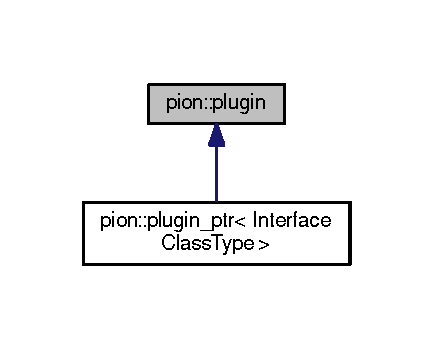
\includegraphics[width=208pt]{classpion_1_1plugin__inherit__graph}
\end{center}
\end{figure}
\subsection*{Classes}
\begin{DoxyCompactItemize}
\item 
struct \hyperlink{structpion_1_1plugin_1_1data__type}{data\-\_\-type}
\end{DoxyCompactItemize}
\subsection*{Public Member Functions}
\begin{DoxyCompactItemize}
\item 
virtual \hyperlink{classpion_1_1plugin_a152b386f2f25db57ac7d87afb543ed91}{$\sim$plugin} ()
\item 
bool \hyperlink{classpion_1_1plugin_a61186fb4cf7ec683e7d9e9f54c507df8}{is\-\_\-open} (void) const 
\begin{DoxyCompactList}\small\item\em returns true if a shared library is loaded/open \end{DoxyCompactList}\item 
std\-::string \hyperlink{classpion_1_1plugin_afbb2e9290143f779b0d01d1ab925cde2}{get\-\_\-plugin\-\_\-name} (void) const 
\begin{DoxyCompactList}\small\item\em returns the name of the plugin that is currently open \end{DoxyCompactList}\item 
void \hyperlink{classpion_1_1plugin_ad2f241076913d3ef35caa298992aa21d}{open} (const std\-::string \&plugin\-\_\-name)
\item 
void \hyperlink{classpion_1_1plugin_aa3848e4da0ef4592079a378f1d81fe12}{open\-\_\-file} (const std\-::string \&plugin\-\_\-file)
\item 
void \hyperlink{classpion_1_1plugin_a4de512c3cdeb3cd9dedd3a49f754cc1a}{close} (void)
\begin{DoxyCompactList}\small\item\em closes plug-\/in library \end{DoxyCompactList}\end{DoxyCompactItemize}
\subsection*{Static Public Member Functions}
\begin{DoxyCompactItemize}
\item 
static bool \hyperlink{classpion_1_1plugin_a8bded1e5b0c6e5008fb62613bf7bed63}{find\-\_\-plugin\-\_\-file} (std\-::string \&path\-\_\-to\-\_\-file, const std\-::string \&name)
\item 
static bool \hyperlink{classpion_1_1plugin_a885fb365fc2fedf251853eb949fcf38a}{find\-\_\-config\-\_\-file} (std\-::string \&path\-\_\-to\-\_\-file, const std\-::string \&name)
\item 
static void \hyperlink{classpion_1_1plugin_a7f070e7afa7b82ee9da454495ee7d659}{add\-\_\-static\-\_\-entry\-\_\-point} (const std\-::string \&plugin\-\_\-name, void $\ast$create\-\_\-func, void $\ast$destroy\-\_\-func)
\item 
static void \hyperlink{classpion_1_1plugin_a424890d78c0e7fe566043b75016bf738}{check\-\_\-cygwin\-\_\-path} (boost\-::filesystem\-::path \&final\-\_\-path, const std\-::string \&path\-\_\-string)
\item 
static void \hyperlink{classpion_1_1plugin_aed4ab06e4aa42456df83e4e3e120dda5}{add\-\_\-plugin\-\_\-directory} (const std\-::string \&dir)
\begin{DoxyCompactList}\small\item\em appends a directory to the plug-\/in search path \end{DoxyCompactList}\item 
static void \hyperlink{classpion_1_1plugin_a797d2923f9495109290755625070f93e}{reset\-\_\-plugin\-\_\-directories} (void)
\begin{DoxyCompactList}\small\item\em clears all directories from the plug-\/in search path \end{DoxyCompactList}\item 
static void \hyperlink{classpion_1_1plugin_add067f91834b99ad73d2ec448aebe33b}{get\-\_\-all\-\_\-plugin\-\_\-names} (std\-::vector$<$ std\-::string $>$ \&plugin\-\_\-names)
\begin{DoxyCompactList}\small\item\em returns a list of all Plugins found in all Plugin directories \end{DoxyCompactList}\end{DoxyCompactItemize}
\subsection*{Protected Member Functions}
\begin{DoxyCompactItemize}
\item 
\hyperlink{classpion_1_1plugin_a132d7077794fd139df56350908805f75}{plugin} (void)
\begin{DoxyCompactList}\small\item\em default constructor is private (use \hyperlink{classpion_1_1plugin__ptr}{plugin\-\_\-ptr} class to create objects) \end{DoxyCompactList}\item 
\hyperlink{classpion_1_1plugin_aa651a50b3be4d9e35ade63b9c9ee66a7}{plugin} (const \hyperlink{classpion_1_1plugin}{plugin} \&p)
\begin{DoxyCompactList}\small\item\em copy constructor \end{DoxyCompactList}\item 
\hyperlink{classpion_1_1plugin}{plugin} \& \hyperlink{classpion_1_1plugin_a31b0610dce244c86d80981240bdb0e62}{operator=} (const \hyperlink{classpion_1_1plugin}{plugin} \&p)
\begin{DoxyCompactList}\small\item\em assignment operator \end{DoxyCompactList}\item 
void $\ast$ \hyperlink{classpion_1_1plugin_a8300881be4224c9331fcbdfc69beb078}{get\-\_\-create\-\_\-function} (void)
\begin{DoxyCompactList}\small\item\em returns a pointer to the plug-\/in's \char`\"{}create object\char`\"{} function \end{DoxyCompactList}\item 
void $\ast$ \hyperlink{classpion_1_1plugin_a473f250fea6e643944aad4484db2b3c9}{get\-\_\-destroy\-\_\-function} (void)
\begin{DoxyCompactList}\small\item\em returns a pointer to the plug-\/in's \char`\"{}destroy object\char`\"{} function \end{DoxyCompactList}\item 
void \hyperlink{classpion_1_1plugin_a6170412055354b9d32c6551baa0bed37}{release\-\_\-data} (void)
\begin{DoxyCompactList}\small\item\em releases the plug-\/in's shared library symbols \end{DoxyCompactList}\item 
void \hyperlink{classpion_1_1plugin_a928793b2ab39387ec1b467ee618fbaa1}{grab\-\_\-data} (const \hyperlink{classpion_1_1plugin}{plugin} \&p)
\begin{DoxyCompactList}\small\item\em grabs a reference to another plug-\/in's shared library symbols \end{DoxyCompactList}\end{DoxyCompactItemize}


\subsection{Detailed Description}
plugin\-: base class for plug-\/in management 

\subsection{Constructor \& Destructor Documentation}
\hypertarget{classpion_1_1plugin_a152b386f2f25db57ac7d87afb543ed91}{\index{pion\-::plugin@{pion\-::plugin}!$\sim$plugin@{$\sim$plugin}}
\index{$\sim$plugin@{$\sim$plugin}!pion::plugin@{pion\-::plugin}}
\subsubsection[{$\sim$plugin}]{\setlength{\rightskip}{0pt plus 5cm}virtual pion\-::plugin\-::$\sim$plugin (
\begin{DoxyParamCaption}
{}
\end{DoxyParamCaption}
)\hspace{0.3cm}{\ttfamily [inline]}, {\ttfamily [virtual]}}}\label{classpion_1_1plugin_a152b386f2f25db57ac7d87afb543ed91}
\hypertarget{classpion_1_1plugin_a132d7077794fd139df56350908805f75}{\index{pion\-::plugin@{pion\-::plugin}!plugin@{plugin}}
\index{plugin@{plugin}!pion::plugin@{pion\-::plugin}}
\subsubsection[{plugin}]{\setlength{\rightskip}{0pt plus 5cm}pion\-::plugin\-::plugin (
\begin{DoxyParamCaption}
\item[{void}]{}
\end{DoxyParamCaption}
)\hspace{0.3cm}{\ttfamily [inline]}, {\ttfamily [protected]}}}\label{classpion_1_1plugin_a132d7077794fd139df56350908805f75}


default constructor is private (use \hyperlink{classpion_1_1plugin__ptr}{plugin\-\_\-ptr} class to create objects) 

\hypertarget{classpion_1_1plugin_aa651a50b3be4d9e35ade63b9c9ee66a7}{\index{pion\-::plugin@{pion\-::plugin}!plugin@{plugin}}
\index{plugin@{plugin}!pion::plugin@{pion\-::plugin}}
\subsubsection[{plugin}]{\setlength{\rightskip}{0pt plus 5cm}pion\-::plugin\-::plugin (
\begin{DoxyParamCaption}
\item[{const {\bf plugin} \&}]{p}
\end{DoxyParamCaption}
)\hspace{0.3cm}{\ttfamily [inline]}, {\ttfamily [protected]}}}\label{classpion_1_1plugin_aa651a50b3be4d9e35ade63b9c9ee66a7}


copy constructor 



\subsection{Member Function Documentation}
\hypertarget{classpion_1_1plugin_aed4ab06e4aa42456df83e4e3e120dda5}{\index{pion\-::plugin@{pion\-::plugin}!add\-\_\-plugin\-\_\-directory@{add\-\_\-plugin\-\_\-directory}}
\index{add\-\_\-plugin\-\_\-directory@{add\-\_\-plugin\-\_\-directory}!pion::plugin@{pion\-::plugin}}
\subsubsection[{add\-\_\-plugin\-\_\-directory}]{\setlength{\rightskip}{0pt plus 5cm}void pion\-::plugin\-::add\-\_\-plugin\-\_\-directory (
\begin{DoxyParamCaption}
\item[{const std\-::string \&}]{dir}
\end{DoxyParamCaption}
)\hspace{0.3cm}{\ttfamily [static]}}}\label{classpion_1_1plugin_aed4ab06e4aa42456df83e4e3e120dda5}


appends a directory to the plug-\/in search path 



References check\-\_\-cygwin\-\_\-path().



Referenced by pion\-::http\-::plugin\-\_\-server\-::load\-\_\-service\-\_\-config().

\hypertarget{classpion_1_1plugin_a7f070e7afa7b82ee9da454495ee7d659}{\index{pion\-::plugin@{pion\-::plugin}!add\-\_\-static\-\_\-entry\-\_\-point@{add\-\_\-static\-\_\-entry\-\_\-point}}
\index{add\-\_\-static\-\_\-entry\-\_\-point@{add\-\_\-static\-\_\-entry\-\_\-point}!pion::plugin@{pion\-::plugin}}
\subsubsection[{add\-\_\-static\-\_\-entry\-\_\-point}]{\setlength{\rightskip}{0pt plus 5cm}void pion\-::plugin\-::add\-\_\-static\-\_\-entry\-\_\-point (
\begin{DoxyParamCaption}
\item[{const std\-::string \&}]{plugin\-\_\-name, }
\item[{void $\ast$}]{create\-\_\-func, }
\item[{void $\ast$}]{destroy\-\_\-func}
\end{DoxyParamCaption}
)\hspace{0.3cm}{\ttfamily [static]}}}\label{classpion_1_1plugin_a7f070e7afa7b82ee9da454495ee7d659}
adds an entry point for a plugin that is statically linked N\-O\-T\-E\-: U\-S\-E \hyperlink{plugin_8hpp_aa24de1879a08dddbc32d19df5b272b0e}{P\-I\-O\-N\-\_\-\-D\-E\-C\-L\-A\-R\-E\-\_\-\-P\-L\-U\-G\-I\-N()} macro instead!!!


\begin{DoxyParams}{Parameters}
{\em plugin\-\_\-name} & the name of the plugin to add \\
\hline
{\em create\-\_\-func} & -\/ pointer to the function to be used in to create plugin object \\
\hline
{\em destroy\-\_\-func} & -\/ pointer to the function to be used to release plugin object \\
\hline
\end{DoxyParams}


References pion\-::plugin\-::data\-\_\-type\-::m\-\_\-create\-\_\-func, pion\-::plugin\-::data\-\_\-type\-::m\-\_\-destroy\-\_\-func, and pion\-::plugin\-::data\-\_\-type\-::m\-\_\-lib\-\_\-handle.

\hypertarget{classpion_1_1plugin_a424890d78c0e7fe566043b75016bf738}{\index{pion\-::plugin@{pion\-::plugin}!check\-\_\-cygwin\-\_\-path@{check\-\_\-cygwin\-\_\-path}}
\index{check\-\_\-cygwin\-\_\-path@{check\-\_\-cygwin\-\_\-path}!pion::plugin@{pion\-::plugin}}
\subsubsection[{check\-\_\-cygwin\-\_\-path}]{\setlength{\rightskip}{0pt plus 5cm}void pion\-::plugin\-::check\-\_\-cygwin\-\_\-path (
\begin{DoxyParamCaption}
\item[{boost\-::filesystem\-::path \&}]{final\-\_\-path, }
\item[{const std\-::string \&}]{path\-\_\-string}
\end{DoxyParamCaption}
)\hspace{0.3cm}{\ttfamily [static]}}}\label{classpion_1_1plugin_a424890d78c0e7fe566043b75016bf738}
updates path for cygwin oddities, if necessary


\begin{DoxyParams}{Parameters}
{\em final\-\_\-path} & path object for the file, will be modified if necessary \\
\hline
{\em start\-\_\-path} & original path to the file. if final\-\_\-path is not valid, this will be appended to P\-I\-O\-N\-\_\-\-C\-Y\-G\-W\-I\-N\-\_\-\-D\-I\-R\-E\-C\-T\-O\-R\-Y to attempt attempt correction of final\-\_\-path for cygwin \\
\hline
\end{DoxyParams}


References P\-I\-O\-N\-\_\-\-C\-Y\-G\-W\-I\-N\-\_\-\-D\-I\-R\-E\-C\-T\-O\-R\-Y.



Referenced by add\-\_\-plugin\-\_\-directory().

\hypertarget{classpion_1_1plugin_a4de512c3cdeb3cd9dedd3a49f754cc1a}{\index{pion\-::plugin@{pion\-::plugin}!close@{close}}
\index{close@{close}!pion::plugin@{pion\-::plugin}}
\subsubsection[{close}]{\setlength{\rightskip}{0pt plus 5cm}void pion\-::plugin\-::close (
\begin{DoxyParamCaption}
\item[{void}]{}
\end{DoxyParamCaption}
)\hspace{0.3cm}{\ttfamily [inline]}}}\label{classpion_1_1plugin_a4de512c3cdeb3cd9dedd3a49f754cc1a}


closes plug-\/in library 

\hypertarget{classpion_1_1plugin_a885fb365fc2fedf251853eb949fcf38a}{\index{pion\-::plugin@{pion\-::plugin}!find\-\_\-config\-\_\-file@{find\-\_\-config\-\_\-file}}
\index{find\-\_\-config\-\_\-file@{find\-\_\-config\-\_\-file}!pion::plugin@{pion\-::plugin}}
\subsubsection[{find\-\_\-config\-\_\-file}]{\setlength{\rightskip}{0pt plus 5cm}static bool pion\-::plugin\-::find\-\_\-config\-\_\-file (
\begin{DoxyParamCaption}
\item[{std\-::string \&}]{path\-\_\-to\-\_\-file, }
\item[{const std\-::string \&}]{name}
\end{DoxyParamCaption}
)\hspace{0.3cm}{\ttfamily [inline]}, {\ttfamily [static]}}}\label{classpion_1_1plugin_a885fb365fc2fedf251853eb949fcf38a}
searches directories for a valid plug-\/in configuration file


\begin{DoxyParams}{Parameters}
{\em path\-\_\-to\-\_\-file} & if found, is set to the complete path to the file \\
\hline
{\em name} & the name of the configuration file to search for \\
\hline
\end{DoxyParams}
\begin{DoxyReturn}{Returns}
true if the configuration file was found 
\end{DoxyReturn}


Referenced by pion\-::http\-::plugin\-\_\-server\-::load\-\_\-service\-\_\-config().

\hypertarget{classpion_1_1plugin_a8bded1e5b0c6e5008fb62613bf7bed63}{\index{pion\-::plugin@{pion\-::plugin}!find\-\_\-plugin\-\_\-file@{find\-\_\-plugin\-\_\-file}}
\index{find\-\_\-plugin\-\_\-file@{find\-\_\-plugin\-\_\-file}!pion::plugin@{pion\-::plugin}}
\subsubsection[{find\-\_\-plugin\-\_\-file}]{\setlength{\rightskip}{0pt plus 5cm}static bool pion\-::plugin\-::find\-\_\-plugin\-\_\-file (
\begin{DoxyParamCaption}
\item[{std\-::string \&}]{path\-\_\-to\-\_\-file, }
\item[{const std\-::string \&}]{name}
\end{DoxyParamCaption}
)\hspace{0.3cm}{\ttfamily [inline]}, {\ttfamily [static]}}}\label{classpion_1_1plugin_a8bded1e5b0c6e5008fb62613bf7bed63}
searches directories for a valid plug-\/in file


\begin{DoxyParams}{Parameters}
{\em path\-\_\-to\-\_\-file} & the path to the plug-\/in file, if found \\
\hline
{\em the} & name name of the plug-\/in to search for \\
\hline
\end{DoxyParams}
\begin{DoxyReturn}{Returns}
true if the plug-\/in file was found 
\end{DoxyReturn}


Referenced by open().

\hypertarget{classpion_1_1plugin_add067f91834b99ad73d2ec448aebe33b}{\index{pion\-::plugin@{pion\-::plugin}!get\-\_\-all\-\_\-plugin\-\_\-names@{get\-\_\-all\-\_\-plugin\-\_\-names}}
\index{get\-\_\-all\-\_\-plugin\-\_\-names@{get\-\_\-all\-\_\-plugin\-\_\-names}!pion::plugin@{pion\-::plugin}}
\subsubsection[{get\-\_\-all\-\_\-plugin\-\_\-names}]{\setlength{\rightskip}{0pt plus 5cm}void pion\-::plugin\-::get\-\_\-all\-\_\-plugin\-\_\-names (
\begin{DoxyParamCaption}
\item[{std\-::vector$<$ std\-::string $>$ \&}]{plugin\-\_\-names}
\end{DoxyParamCaption}
)\hspace{0.3cm}{\ttfamily [static]}}}\label{classpion_1_1plugin_add067f91834b99ad73d2ec448aebe33b}


returns a list of all Plugins found in all Plugin directories 



References get\-\_\-plugin\-\_\-name(), pion\-::plugin\-::data\-\_\-type\-::m\-\_\-lib\-\_\-handle, and pion\-::plugin\-::data\-\_\-type\-::m\-\_\-plugin\-\_\-name.

\hypertarget{classpion_1_1plugin_a8300881be4224c9331fcbdfc69beb078}{\index{pion\-::plugin@{pion\-::plugin}!get\-\_\-create\-\_\-function@{get\-\_\-create\-\_\-function}}
\index{get\-\_\-create\-\_\-function@{get\-\_\-create\-\_\-function}!pion::plugin@{pion\-::plugin}}
\subsubsection[{get\-\_\-create\-\_\-function}]{\setlength{\rightskip}{0pt plus 5cm}void$\ast$ pion\-::plugin\-::get\-\_\-create\-\_\-function (
\begin{DoxyParamCaption}
\item[{void}]{}
\end{DoxyParamCaption}
)\hspace{0.3cm}{\ttfamily [inline]}, {\ttfamily [protected]}}}\label{classpion_1_1plugin_a8300881be4224c9331fcbdfc69beb078}


returns a pointer to the plug-\/in's \char`\"{}create object\char`\"{} function 



Referenced by pion\-::plugin\-\_\-ptr$<$ Interface\-Class\-Type $>$\-::create().

\hypertarget{classpion_1_1plugin_a473f250fea6e643944aad4484db2b3c9}{\index{pion\-::plugin@{pion\-::plugin}!get\-\_\-destroy\-\_\-function@{get\-\_\-destroy\-\_\-function}}
\index{get\-\_\-destroy\-\_\-function@{get\-\_\-destroy\-\_\-function}!pion::plugin@{pion\-::plugin}}
\subsubsection[{get\-\_\-destroy\-\_\-function}]{\setlength{\rightskip}{0pt plus 5cm}void$\ast$ pion\-::plugin\-::get\-\_\-destroy\-\_\-function (
\begin{DoxyParamCaption}
\item[{void}]{}
\end{DoxyParamCaption}
)\hspace{0.3cm}{\ttfamily [inline]}, {\ttfamily [protected]}}}\label{classpion_1_1plugin_a473f250fea6e643944aad4484db2b3c9}


returns a pointer to the plug-\/in's \char`\"{}destroy object\char`\"{} function 



Referenced by pion\-::plugin\-\_\-ptr$<$ Interface\-Class\-Type $>$\-::destroy().

\hypertarget{classpion_1_1plugin_afbb2e9290143f779b0d01d1ab925cde2}{\index{pion\-::plugin@{pion\-::plugin}!get\-\_\-plugin\-\_\-name@{get\-\_\-plugin\-\_\-name}}
\index{get\-\_\-plugin\-\_\-name@{get\-\_\-plugin\-\_\-name}!pion::plugin@{pion\-::plugin}}
\subsubsection[{get\-\_\-plugin\-\_\-name}]{\setlength{\rightskip}{0pt plus 5cm}std\-::string pion\-::plugin\-::get\-\_\-plugin\-\_\-name (
\begin{DoxyParamCaption}
\item[{void}]{}
\end{DoxyParamCaption}
) const\hspace{0.3cm}{\ttfamily [inline]}}}\label{classpion_1_1plugin_afbb2e9290143f779b0d01d1ab925cde2}


returns the name of the plugin that is currently open 



Referenced by get\-\_\-all\-\_\-plugin\-\_\-names(), and open\-\_\-file().

\hypertarget{classpion_1_1plugin_a928793b2ab39387ec1b467ee618fbaa1}{\index{pion\-::plugin@{pion\-::plugin}!grab\-\_\-data@{grab\-\_\-data}}
\index{grab\-\_\-data@{grab\-\_\-data}!pion::plugin@{pion\-::plugin}}
\subsubsection[{grab\-\_\-data}]{\setlength{\rightskip}{0pt plus 5cm}void pion\-::plugin\-::grab\-\_\-data (
\begin{DoxyParamCaption}
\item[{const {\bf plugin} \&}]{p}
\end{DoxyParamCaption}
)\hspace{0.3cm}{\ttfamily [protected]}}}\label{classpion_1_1plugin_a928793b2ab39387ec1b467ee618fbaa1}


grabs a reference to another plug-\/in's shared library symbols 



References pion\-::plugin\-::data\-\_\-type\-::m\-\_\-references, and release\-\_\-data().



Referenced by pion\-::plugin\-\_\-ptr$<$ Interface\-Class\-Type $>$\-::operator=().

\hypertarget{classpion_1_1plugin_a61186fb4cf7ec683e7d9e9f54c507df8}{\index{pion\-::plugin@{pion\-::plugin}!is\-\_\-open@{is\-\_\-open}}
\index{is\-\_\-open@{is\-\_\-open}!pion::plugin@{pion\-::plugin}}
\subsubsection[{is\-\_\-open}]{\setlength{\rightskip}{0pt plus 5cm}bool pion\-::plugin\-::is\-\_\-open (
\begin{DoxyParamCaption}
\item[{void}]{}
\end{DoxyParamCaption}
) const\hspace{0.3cm}{\ttfamily [inline]}}}\label{classpion_1_1plugin_a61186fb4cf7ec683e7d9e9f54c507df8}


returns true if a shared library is loaded/open 

\hypertarget{classpion_1_1plugin_ad2f241076913d3ef35caa298992aa21d}{\index{pion\-::plugin@{pion\-::plugin}!open@{open}}
\index{open@{open}!pion::plugin@{pion\-::plugin}}
\subsubsection[{open}]{\setlength{\rightskip}{0pt plus 5cm}void pion\-::plugin\-::open (
\begin{DoxyParamCaption}
\item[{const std\-::string \&}]{plugin\-\_\-name}
\end{DoxyParamCaption}
)}}\label{classpion_1_1plugin_ad2f241076913d3ef35caa298992aa21d}
opens plug-\/in library within a shared object file. If the library is already being used by another plugin object, then the existing code will be re-\/used and the reference count will be increased. Beware that this does N\-O\-T check the plug-\/in's base class (Interface\-Class\-Type), so you must be careful to ensure that the namespace is unique between plug-\/ins that have different base classes. If the plug-\/in's name matches an existing plug-\/in of a different base class, the resulting behavior is undefined (it will probably crash your program).


\begin{DoxyParams}{Parameters}
{\em plugin\-\_\-name} & name of the plug-\/in library to open (without extension, etc.) \\
\hline
\end{DoxyParams}


References find\-\_\-plugin\-\_\-file(), pion\-::plugin\-::data\-\_\-type\-::m\-\_\-references, open\-\_\-file(), and release\-\_\-data().



Referenced by pion\-::plugin\-\_\-manager$<$ Plugin\-Type $>$\-::load().

\hypertarget{classpion_1_1plugin_aa3848e4da0ef4592079a378f1d81fe12}{\index{pion\-::plugin@{pion\-::plugin}!open\-\_\-file@{open\-\_\-file}}
\index{open\-\_\-file@{open\-\_\-file}!pion::plugin@{pion\-::plugin}}
\subsubsection[{open\-\_\-file}]{\setlength{\rightskip}{0pt plus 5cm}void pion\-::plugin\-::open\-\_\-file (
\begin{DoxyParamCaption}
\item[{const std\-::string \&}]{plugin\-\_\-file}
\end{DoxyParamCaption}
)}}\label{classpion_1_1plugin_aa3848e4da0ef4592079a378f1d81fe12}
opens plug-\/in library within a shared object file. If the library is already being used by another plugin object, then the existing code will be re-\/used and the reference count will be increased. Beware that this does N\-O\-T check the plug-\/in's base class (Interface\-Class\-Type), so you must be careful to ensure that the namespace is unique between plug-\/ins that have different base classes. If the plug-\/in's name matches an existing plug-\/in of a different base class, the resulting behavior is undefined (it will probably crash your program).


\begin{DoxyParams}{Parameters}
{\em plugin\-\_\-file} & shared object file containing the plugin code \\
\hline
\end{DoxyParams}


References get\-\_\-plugin\-\_\-name(), pion\-::plugin\-::data\-\_\-type\-::m\-\_\-plugin\-\_\-name, pion\-::plugin\-::data\-\_\-type\-::m\-\_\-references, and release\-\_\-data().



Referenced by open().

\hypertarget{classpion_1_1plugin_a31b0610dce244c86d80981240bdb0e62}{\index{pion\-::plugin@{pion\-::plugin}!operator=@{operator=}}
\index{operator=@{operator=}!pion::plugin@{pion\-::plugin}}
\subsubsection[{operator=}]{\setlength{\rightskip}{0pt plus 5cm}{\bf plugin}\& pion\-::plugin\-::operator= (
\begin{DoxyParamCaption}
\item[{const {\bf plugin} \&}]{p}
\end{DoxyParamCaption}
)\hspace{0.3cm}{\ttfamily [inline]}, {\ttfamily [protected]}}}\label{classpion_1_1plugin_a31b0610dce244c86d80981240bdb0e62}


assignment operator 

\hypertarget{classpion_1_1plugin_a6170412055354b9d32c6551baa0bed37}{\index{pion\-::plugin@{pion\-::plugin}!release\-\_\-data@{release\-\_\-data}}
\index{release\-\_\-data@{release\-\_\-data}!pion::plugin@{pion\-::plugin}}
\subsubsection[{release\-\_\-data}]{\setlength{\rightskip}{0pt plus 5cm}void pion\-::plugin\-::release\-\_\-data (
\begin{DoxyParamCaption}
\item[{void}]{}
\end{DoxyParamCaption}
)\hspace{0.3cm}{\ttfamily [protected]}}}\label{classpion_1_1plugin_a6170412055354b9d32c6551baa0bed37}


releases the plug-\/in's shared library symbols 



References pion\-::plugin\-::data\-\_\-type\-::m\-\_\-lib\-\_\-handle, pion\-::plugin\-::data\-\_\-type\-::m\-\_\-plugin\-\_\-name, and pion\-::plugin\-::data\-\_\-type\-::m\-\_\-references.



Referenced by grab\-\_\-data(), open(), and open\-\_\-file().

\hypertarget{classpion_1_1plugin_a797d2923f9495109290755625070f93e}{\index{pion\-::plugin@{pion\-::plugin}!reset\-\_\-plugin\-\_\-directories@{reset\-\_\-plugin\-\_\-directories}}
\index{reset\-\_\-plugin\-\_\-directories@{reset\-\_\-plugin\-\_\-directories}!pion::plugin@{pion\-::plugin}}
\subsubsection[{reset\-\_\-plugin\-\_\-directories}]{\setlength{\rightskip}{0pt plus 5cm}void pion\-::plugin\-::reset\-\_\-plugin\-\_\-directories (
\begin{DoxyParamCaption}
\item[{void}]{}
\end{DoxyParamCaption}
)\hspace{0.3cm}{\ttfamily [static]}}}\label{classpion_1_1plugin_a797d2923f9495109290755625070f93e}


clears all directories from the plug-\/in search path 



The documentation for this class was generated from the following files\-:\begin{DoxyCompactItemize}
\item 
include/pion/\hyperlink{plugin_8hpp}{plugin.\-hpp}\item 
src/\hyperlink{plugin_8cpp}{plugin.\-cpp}\end{DoxyCompactItemize}

\hypertarget{classpion_1_1plugin__instance__ptr}{\section{pion\-:\-:plugin\-\_\-instance\-\_\-ptr$<$ Interface\-Class\-Type $>$ Class Template Reference}
\label{classpion_1_1plugin__instance__ptr}\index{pion\-::plugin\-\_\-instance\-\_\-ptr$<$ Interface\-Class\-Type $>$@{pion\-::plugin\-\_\-instance\-\_\-ptr$<$ Interface\-Class\-Type $>$}}
}


{\ttfamily \#include $<$plugin.\-hpp$>$}



Inheritance diagram for pion\-:\-:plugin\-\_\-instance\-\_\-ptr$<$ Interface\-Class\-Type $>$\-:
\nopagebreak
\begin{figure}[H]
\begin{center}
\leavevmode
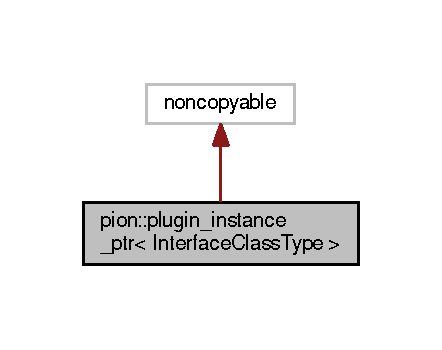
\includegraphics[width=212pt]{classpion_1_1plugin__instance__ptr__inherit__graph}
\end{center}
\end{figure}


Collaboration diagram for pion\-:\-:plugin\-\_\-instance\-\_\-ptr$<$ Interface\-Class\-Type $>$\-:
\nopagebreak
\begin{figure}[H]
\begin{center}
\leavevmode
\includegraphics[width=212pt]{classpion_1_1plugin__instance__ptr__coll__graph}
\end{center}
\end{figure}
\subsection*{Public Member Functions}
\begin{DoxyCompactItemize}
\item 
\hyperlink{classpion_1_1plugin__instance__ptr_a79eb26b5a1ff329e4893c644a625dcc6}{plugin\-\_\-instance\-\_\-ptr} (void)
\begin{DoxyCompactList}\small\item\em default constructor \& destructor \end{DoxyCompactList}\item 
virtual \hyperlink{classpion_1_1plugin__instance__ptr_a6567dda0004c26eba60a6c714d52c696}{$\sim$plugin\-\_\-instance\-\_\-ptr} ()
\begin{DoxyCompactList}\small\item\em virtual destructor / may be extended \end{DoxyCompactList}\item 
void \hyperlink{classpion_1_1plugin__instance__ptr_a3c6d24f4501a0e1838e5bedd34e20372}{reset} (void)
\begin{DoxyCompactList}\small\item\em reset the instance pointer \end{DoxyCompactList}\item 
void \hyperlink{classpion_1_1plugin__instance__ptr_a7cc8432ad7e88298c719e9b41007e93d}{create} (const std\-::string \&plugin\-\_\-type)
\begin{DoxyCompactList}\small\item\em create a new instance of the given plugin\-\_\-type \end{DoxyCompactList}\item 
bool \hyperlink{classpion_1_1plugin__instance__ptr_ac4655ccda770223a852233c7c9ffb0d0}{empty} (void) const 
\begin{DoxyCompactList}\small\item\em returns true if pointer is empty \end{DoxyCompactList}\item 
Interface\-Class\-Type $\ast$ \hyperlink{classpion_1_1plugin__instance__ptr_a30f57ad0560c0cbdd0f00f345cd3a41a}{get} (void)
\begin{DoxyCompactList}\small\item\em return a raw pointer to the instance \end{DoxyCompactList}\item 
Interface\-Class\-Type \& \hyperlink{classpion_1_1plugin__instance__ptr_af1919987100381b912d49144f75c46fe}{operator$\ast$} (void)
\begin{DoxyCompactList}\small\item\em return a reference to the instance \end{DoxyCompactList}\item 
const Interface\-Class\-Type \& \hyperlink{classpion_1_1plugin__instance__ptr_a0ed2270357907c47060b5c0bd14cb6fb}{operator$\ast$} (void) const 
\begin{DoxyCompactList}\small\item\em return a const reference to the instance \end{DoxyCompactList}\item 
Interface\-Class\-Type $\ast$ \hyperlink{classpion_1_1plugin__instance__ptr_a84f65b0841e70a2a6017792d5749390e}{operator-\/$>$} (void)
\begin{DoxyCompactList}\small\item\em return a reference to the instance \end{DoxyCompactList}\item 
const Interface\-Class\-Type $\ast$ \hyperlink{classpion_1_1plugin__instance__ptr_a26b25d3a76f14a22636727ed774eac29}{operator-\/$>$} (void) const 
\begin{DoxyCompactList}\small\item\em return a const reference to the instance \end{DoxyCompactList}\end{DoxyCompactItemize}
\subsection*{Protected Attributes}
\begin{DoxyCompactItemize}
\item 
\hyperlink{classpion_1_1plugin__ptr}{plugin\-\_\-ptr}$<$ Interface\-Class\-Type $>$ \hyperlink{classpion_1_1plugin__instance__ptr_a65856c5fbd856e3c106e3ae708369109}{m\-\_\-plugin\-\_\-ptr}
\begin{DoxyCompactList}\small\item\em smart pointer that manages the plugin's dynamic object code \end{DoxyCompactList}\item 
Interface\-Class\-Type $\ast$ \hyperlink{classpion_1_1plugin__instance__ptr_a414a8f8e915a41caa94aca991cbb775e}{m\-\_\-instance\-\_\-ptr}
\begin{DoxyCompactList}\small\item\em raw pointer to the plugin instance \end{DoxyCompactList}\end{DoxyCompactItemize}


\subsection{Detailed Description}
\subsubsection*{template$<$typename Interface\-Class\-Type$>$class pion\-::plugin\-\_\-instance\-\_\-ptr$<$ Interface\-Class\-Type $>$}

\hyperlink{classpion_1_1plugin__instance__ptr}{plugin\-\_\-instance\-\_\-ptr}\-: smart pointer that manages a plug-\/in instance 

\subsection{Constructor \& Destructor Documentation}
\hypertarget{classpion_1_1plugin__instance__ptr_a79eb26b5a1ff329e4893c644a625dcc6}{\index{pion\-::plugin\-\_\-instance\-\_\-ptr@{pion\-::plugin\-\_\-instance\-\_\-ptr}!plugin\-\_\-instance\-\_\-ptr@{plugin\-\_\-instance\-\_\-ptr}}
\index{plugin\-\_\-instance\-\_\-ptr@{plugin\-\_\-instance\-\_\-ptr}!pion::plugin_instance_ptr@{pion\-::plugin\-\_\-instance\-\_\-ptr}}
\subsubsection[{plugin\-\_\-instance\-\_\-ptr}]{\setlength{\rightskip}{0pt plus 5cm}template$<$typename Interface\-Class\-Type $>$ {\bf pion\-::plugin\-\_\-instance\-\_\-ptr}$<$ Interface\-Class\-Type $>$\-::{\bf plugin\-\_\-instance\-\_\-ptr} (
\begin{DoxyParamCaption}
\item[{void}]{}
\end{DoxyParamCaption}
)\hspace{0.3cm}{\ttfamily [inline]}}}\label{classpion_1_1plugin__instance__ptr_a79eb26b5a1ff329e4893c644a625dcc6}


default constructor \& destructor 

\hypertarget{classpion_1_1plugin__instance__ptr_a6567dda0004c26eba60a6c714d52c696}{\index{pion\-::plugin\-\_\-instance\-\_\-ptr@{pion\-::plugin\-\_\-instance\-\_\-ptr}!$\sim$plugin\-\_\-instance\-\_\-ptr@{$\sim$plugin\-\_\-instance\-\_\-ptr}}
\index{$\sim$plugin\-\_\-instance\-\_\-ptr@{$\sim$plugin\-\_\-instance\-\_\-ptr}!pion::plugin_instance_ptr@{pion\-::plugin\-\_\-instance\-\_\-ptr}}
\subsubsection[{$\sim$plugin\-\_\-instance\-\_\-ptr}]{\setlength{\rightskip}{0pt plus 5cm}template$<$typename Interface\-Class\-Type $>$ virtual {\bf pion\-::plugin\-\_\-instance\-\_\-ptr}$<$ Interface\-Class\-Type $>$\-::$\sim${\bf plugin\-\_\-instance\-\_\-ptr} (
\begin{DoxyParamCaption}
{}
\end{DoxyParamCaption}
)\hspace{0.3cm}{\ttfamily [inline]}, {\ttfamily [virtual]}}}\label{classpion_1_1plugin__instance__ptr_a6567dda0004c26eba60a6c714d52c696}


virtual destructor / may be extended 



References pion\-::plugin\-\_\-instance\-\_\-ptr$<$ Interface\-Class\-Type $>$\-::reset().



\subsection{Member Function Documentation}
\hypertarget{classpion_1_1plugin__instance__ptr_a7cc8432ad7e88298c719e9b41007e93d}{\index{pion\-::plugin\-\_\-instance\-\_\-ptr@{pion\-::plugin\-\_\-instance\-\_\-ptr}!create@{create}}
\index{create@{create}!pion::plugin_instance_ptr@{pion\-::plugin\-\_\-instance\-\_\-ptr}}
\subsubsection[{create}]{\setlength{\rightskip}{0pt plus 5cm}template$<$typename Interface\-Class\-Type $>$ void {\bf pion\-::plugin\-\_\-instance\-\_\-ptr}$<$ Interface\-Class\-Type $>$\-::create (
\begin{DoxyParamCaption}
\item[{const std\-::string \&}]{plugin\-\_\-type}
\end{DoxyParamCaption}
)\hspace{0.3cm}{\ttfamily [inline]}}}\label{classpion_1_1plugin__instance__ptr_a7cc8432ad7e88298c719e9b41007e93d}


create a new instance of the given plugin\-\_\-type 



References pion\-::plugin\-\_\-instance\-\_\-ptr$<$ Interface\-Class\-Type $>$\-::m\-\_\-instance\-\_\-ptr, pion\-::plugin\-\_\-instance\-\_\-ptr$<$ Interface\-Class\-Type $>$\-::m\-\_\-plugin\-\_\-ptr, and pion\-::plugin\-\_\-instance\-\_\-ptr$<$ Interface\-Class\-Type $>$\-::reset().

\hypertarget{classpion_1_1plugin__instance__ptr_ac4655ccda770223a852233c7c9ffb0d0}{\index{pion\-::plugin\-\_\-instance\-\_\-ptr@{pion\-::plugin\-\_\-instance\-\_\-ptr}!empty@{empty}}
\index{empty@{empty}!pion::plugin_instance_ptr@{pion\-::plugin\-\_\-instance\-\_\-ptr}}
\subsubsection[{empty}]{\setlength{\rightskip}{0pt plus 5cm}template$<$typename Interface\-Class\-Type $>$ bool {\bf pion\-::plugin\-\_\-instance\-\_\-ptr}$<$ Interface\-Class\-Type $>$\-::empty (
\begin{DoxyParamCaption}
\item[{void}]{}
\end{DoxyParamCaption}
) const\hspace{0.3cm}{\ttfamily [inline]}}}\label{classpion_1_1plugin__instance__ptr_ac4655ccda770223a852233c7c9ffb0d0}


returns true if pointer is empty 



References pion\-::plugin\-\_\-instance\-\_\-ptr$<$ Interface\-Class\-Type $>$\-::m\-\_\-instance\-\_\-ptr.

\hypertarget{classpion_1_1plugin__instance__ptr_a30f57ad0560c0cbdd0f00f345cd3a41a}{\index{pion\-::plugin\-\_\-instance\-\_\-ptr@{pion\-::plugin\-\_\-instance\-\_\-ptr}!get@{get}}
\index{get@{get}!pion::plugin_instance_ptr@{pion\-::plugin\-\_\-instance\-\_\-ptr}}
\subsubsection[{get}]{\setlength{\rightskip}{0pt plus 5cm}template$<$typename Interface\-Class\-Type $>$ Interface\-Class\-Type$\ast$ {\bf pion\-::plugin\-\_\-instance\-\_\-ptr}$<$ Interface\-Class\-Type $>$\-::get (
\begin{DoxyParamCaption}
\item[{void}]{}
\end{DoxyParamCaption}
)\hspace{0.3cm}{\ttfamily [inline]}}}\label{classpion_1_1plugin__instance__ptr_a30f57ad0560c0cbdd0f00f345cd3a41a}


return a raw pointer to the instance 



References pion\-::plugin\-\_\-instance\-\_\-ptr$<$ Interface\-Class\-Type $>$\-::m\-\_\-instance\-\_\-ptr.

\hypertarget{classpion_1_1plugin__instance__ptr_af1919987100381b912d49144f75c46fe}{\index{pion\-::plugin\-\_\-instance\-\_\-ptr@{pion\-::plugin\-\_\-instance\-\_\-ptr}!operator$\ast$@{operator$\ast$}}
\index{operator$\ast$@{operator$\ast$}!pion::plugin_instance_ptr@{pion\-::plugin\-\_\-instance\-\_\-ptr}}
\subsubsection[{operator$\ast$}]{\setlength{\rightskip}{0pt plus 5cm}template$<$typename Interface\-Class\-Type $>$ Interface\-Class\-Type\& {\bf pion\-::plugin\-\_\-instance\-\_\-ptr}$<$ Interface\-Class\-Type $>$\-::operator$\ast$ (
\begin{DoxyParamCaption}
\item[{void}]{}
\end{DoxyParamCaption}
)\hspace{0.3cm}{\ttfamily [inline]}}}\label{classpion_1_1plugin__instance__ptr_af1919987100381b912d49144f75c46fe}


return a reference to the instance 



References pion\-::plugin\-\_\-instance\-\_\-ptr$<$ Interface\-Class\-Type $>$\-::m\-\_\-instance\-\_\-ptr.

\hypertarget{classpion_1_1plugin__instance__ptr_a0ed2270357907c47060b5c0bd14cb6fb}{\index{pion\-::plugin\-\_\-instance\-\_\-ptr@{pion\-::plugin\-\_\-instance\-\_\-ptr}!operator$\ast$@{operator$\ast$}}
\index{operator$\ast$@{operator$\ast$}!pion::plugin_instance_ptr@{pion\-::plugin\-\_\-instance\-\_\-ptr}}
\subsubsection[{operator$\ast$}]{\setlength{\rightskip}{0pt plus 5cm}template$<$typename Interface\-Class\-Type $>$ const Interface\-Class\-Type\& {\bf pion\-::plugin\-\_\-instance\-\_\-ptr}$<$ Interface\-Class\-Type $>$\-::operator$\ast$ (
\begin{DoxyParamCaption}
\item[{void}]{}
\end{DoxyParamCaption}
) const\hspace{0.3cm}{\ttfamily [inline]}}}\label{classpion_1_1plugin__instance__ptr_a0ed2270357907c47060b5c0bd14cb6fb}


return a const reference to the instance 



References pion\-::plugin\-\_\-instance\-\_\-ptr$<$ Interface\-Class\-Type $>$\-::m\-\_\-instance\-\_\-ptr.

\hypertarget{classpion_1_1plugin__instance__ptr_a84f65b0841e70a2a6017792d5749390e}{\index{pion\-::plugin\-\_\-instance\-\_\-ptr@{pion\-::plugin\-\_\-instance\-\_\-ptr}!operator-\/$>$@{operator-\/$>$}}
\index{operator-\/$>$@{operator-\/$>$}!pion::plugin_instance_ptr@{pion\-::plugin\-\_\-instance\-\_\-ptr}}
\subsubsection[{operator-\/$>$}]{\setlength{\rightskip}{0pt plus 5cm}template$<$typename Interface\-Class\-Type $>$ Interface\-Class\-Type$\ast$ {\bf pion\-::plugin\-\_\-instance\-\_\-ptr}$<$ Interface\-Class\-Type $>$\-::operator-\/$>$ (
\begin{DoxyParamCaption}
\item[{void}]{}
\end{DoxyParamCaption}
)\hspace{0.3cm}{\ttfamily [inline]}}}\label{classpion_1_1plugin__instance__ptr_a84f65b0841e70a2a6017792d5749390e}


return a reference to the instance 



References pion\-::plugin\-\_\-instance\-\_\-ptr$<$ Interface\-Class\-Type $>$\-::m\-\_\-instance\-\_\-ptr.

\hypertarget{classpion_1_1plugin__instance__ptr_a26b25d3a76f14a22636727ed774eac29}{\index{pion\-::plugin\-\_\-instance\-\_\-ptr@{pion\-::plugin\-\_\-instance\-\_\-ptr}!operator-\/$>$@{operator-\/$>$}}
\index{operator-\/$>$@{operator-\/$>$}!pion::plugin_instance_ptr@{pion\-::plugin\-\_\-instance\-\_\-ptr}}
\subsubsection[{operator-\/$>$}]{\setlength{\rightskip}{0pt plus 5cm}template$<$typename Interface\-Class\-Type $>$ const Interface\-Class\-Type$\ast$ {\bf pion\-::plugin\-\_\-instance\-\_\-ptr}$<$ Interface\-Class\-Type $>$\-::operator-\/$>$ (
\begin{DoxyParamCaption}
\item[{void}]{}
\end{DoxyParamCaption}
) const\hspace{0.3cm}{\ttfamily [inline]}}}\label{classpion_1_1plugin__instance__ptr_a26b25d3a76f14a22636727ed774eac29}


return a const reference to the instance 



References pion\-::plugin\-\_\-instance\-\_\-ptr$<$ Interface\-Class\-Type $>$\-::m\-\_\-instance\-\_\-ptr.

\hypertarget{classpion_1_1plugin__instance__ptr_a3c6d24f4501a0e1838e5bedd34e20372}{\index{pion\-::plugin\-\_\-instance\-\_\-ptr@{pion\-::plugin\-\_\-instance\-\_\-ptr}!reset@{reset}}
\index{reset@{reset}!pion::plugin_instance_ptr@{pion\-::plugin\-\_\-instance\-\_\-ptr}}
\subsubsection[{reset}]{\setlength{\rightskip}{0pt plus 5cm}template$<$typename Interface\-Class\-Type $>$ void {\bf pion\-::plugin\-\_\-instance\-\_\-ptr}$<$ Interface\-Class\-Type $>$\-::reset (
\begin{DoxyParamCaption}
\item[{void}]{}
\end{DoxyParamCaption}
)\hspace{0.3cm}{\ttfamily [inline]}}}\label{classpion_1_1plugin__instance__ptr_a3c6d24f4501a0e1838e5bedd34e20372}


reset the instance pointer 



References pion\-::plugin\-\_\-instance\-\_\-ptr$<$ Interface\-Class\-Type $>$\-::m\-\_\-instance\-\_\-ptr, and pion\-::plugin\-\_\-instance\-\_\-ptr$<$ Interface\-Class\-Type $>$\-::m\-\_\-plugin\-\_\-ptr.



Referenced by pion\-::plugin\-\_\-instance\-\_\-ptr$<$ Interface\-Class\-Type $>$\-::create(), and pion\-::plugin\-\_\-instance\-\_\-ptr$<$ Interface\-Class\-Type $>$\-::$\sim$plugin\-\_\-instance\-\_\-ptr().



\subsection{Member Data Documentation}
\hypertarget{classpion_1_1plugin__instance__ptr_a414a8f8e915a41caa94aca991cbb775e}{\index{pion\-::plugin\-\_\-instance\-\_\-ptr@{pion\-::plugin\-\_\-instance\-\_\-ptr}!m\-\_\-instance\-\_\-ptr@{m\-\_\-instance\-\_\-ptr}}
\index{m\-\_\-instance\-\_\-ptr@{m\-\_\-instance\-\_\-ptr}!pion::plugin_instance_ptr@{pion\-::plugin\-\_\-instance\-\_\-ptr}}
\subsubsection[{m\-\_\-instance\-\_\-ptr}]{\setlength{\rightskip}{0pt plus 5cm}template$<$typename Interface\-Class\-Type $>$ Interface\-Class\-Type$\ast$ {\bf pion\-::plugin\-\_\-instance\-\_\-ptr}$<$ Interface\-Class\-Type $>$\-::m\-\_\-instance\-\_\-ptr\hspace{0.3cm}{\ttfamily [protected]}}}\label{classpion_1_1plugin__instance__ptr_a414a8f8e915a41caa94aca991cbb775e}


raw pointer to the plugin instance 



Referenced by pion\-::plugin\-\_\-instance\-\_\-ptr$<$ Interface\-Class\-Type $>$\-::create(), pion\-::plugin\-\_\-instance\-\_\-ptr$<$ Interface\-Class\-Type $>$\-::empty(), pion\-::plugin\-\_\-instance\-\_\-ptr$<$ Interface\-Class\-Type $>$\-::get(), pion\-::plugin\-\_\-instance\-\_\-ptr$<$ Interface\-Class\-Type $>$\-::operator$\ast$(), pion\-::plugin\-\_\-instance\-\_\-ptr$<$ Interface\-Class\-Type $>$\-::operator-\/$>$(), and pion\-::plugin\-\_\-instance\-\_\-ptr$<$ Interface\-Class\-Type $>$\-::reset().

\hypertarget{classpion_1_1plugin__instance__ptr_a65856c5fbd856e3c106e3ae708369109}{\index{pion\-::plugin\-\_\-instance\-\_\-ptr@{pion\-::plugin\-\_\-instance\-\_\-ptr}!m\-\_\-plugin\-\_\-ptr@{m\-\_\-plugin\-\_\-ptr}}
\index{m\-\_\-plugin\-\_\-ptr@{m\-\_\-plugin\-\_\-ptr}!pion::plugin_instance_ptr@{pion\-::plugin\-\_\-instance\-\_\-ptr}}
\subsubsection[{m\-\_\-plugin\-\_\-ptr}]{\setlength{\rightskip}{0pt plus 5cm}template$<$typename Interface\-Class\-Type $>$ {\bf plugin\-\_\-ptr}$<$Interface\-Class\-Type$>$ {\bf pion\-::plugin\-\_\-instance\-\_\-ptr}$<$ Interface\-Class\-Type $>$\-::m\-\_\-plugin\-\_\-ptr\hspace{0.3cm}{\ttfamily [protected]}}}\label{classpion_1_1plugin__instance__ptr_a65856c5fbd856e3c106e3ae708369109}


smart pointer that manages the plugin's dynamic object code 



Referenced by pion\-::plugin\-\_\-instance\-\_\-ptr$<$ Interface\-Class\-Type $>$\-::create(), and pion\-::plugin\-\_\-instance\-\_\-ptr$<$ Interface\-Class\-Type $>$\-::reset().



The documentation for this class was generated from the following file\-:\begin{DoxyCompactItemize}
\item 
include/pion/\hyperlink{plugin_8hpp}{plugin.\-hpp}\end{DoxyCompactItemize}

\hypertarget{classpion_1_1plugin__manager}{\section{pion\-:\-:plugin\-\_\-manager$<$ Plugin\-Type $>$ Class Template Reference}
\label{classpion_1_1plugin__manager}\index{pion\-::plugin\-\_\-manager$<$ Plugin\-Type $>$@{pion\-::plugin\-\_\-manager$<$ Plugin\-Type $>$}}
}


{\ttfamily \#include $<$plugin\-\_\-manager.\-hpp$>$}



Collaboration diagram for pion\-:\-:plugin\-\_\-manager$<$ Plugin\-Type $>$\-:
\nopagebreak
\begin{figure}[H]
\begin{center}
\leavevmode
\includegraphics[width=230pt]{classpion_1_1plugin__manager__coll__graph}
\end{center}
\end{figure}
\subsection*{Classes}
\begin{DoxyCompactItemize}
\item 
class \hyperlink{classpion_1_1plugin__manager_1_1map__type}{map\-\_\-type}
\begin{DoxyCompactList}\small\item\em data type that maps identifiers to plug-\/in objects \end{DoxyCompactList}\end{DoxyCompactItemize}
\subsection*{Public Types}
\begin{DoxyCompactItemize}
\item 
typedef boost\-::function1$<$ void, \\*
Plugin\-Type $\ast$ $>$ \hyperlink{classpion_1_1plugin__manager_a275b88a2c9f7c89d6d737c1b444be8b2}{Plugin\-Run\-Function}
\begin{DoxyCompactList}\small\item\em data type for a function that may be called by the \hyperlink{classpion_1_1plugin__manager_a1c2f6105acfcfcf1b742aecab122a368}{run()} method \end{DoxyCompactList}\item 
typedef boost\-::function1\\*
$<$ boost\-::uint64\-\_\-t, const \\*
Plugin\-Type $\ast$ $>$ \hyperlink{classpion_1_1plugin__manager_a1e6a4223438c74e4e928401f734d2e0c}{Plugin\-Stat\-Function}
\begin{DoxyCompactList}\small\item\em data type for a function that may be called by the get\-Stat() method \end{DoxyCompactList}\end{DoxyCompactItemize}
\subsection*{Public Member Functions}
\begin{DoxyCompactItemize}
\item 
\hyperlink{classpion_1_1plugin__manager_a6f451cdb1f4ea91b954e5dd453a827d3}{plugin\-\_\-manager} (void)
\begin{DoxyCompactList}\small\item\em default constructor \end{DoxyCompactList}\item 
virtual \hyperlink{classpion_1_1plugin__manager_aff2f27834dee6eb0087e68f2af86b9e9}{$\sim$plugin\-\_\-manager} ()
\begin{DoxyCompactList}\small\item\em default destructor \end{DoxyCompactList}\item 
void \hyperlink{classpion_1_1plugin__manager_ac56a5e432352d1b9c2a4853ce82a5a8c}{clear} (void)
\begin{DoxyCompactList}\small\item\em clears all the plug-\/in objects being managed \end{DoxyCompactList}\item 
bool \hyperlink{classpion_1_1plugin__manager_adee5498ef23acb797355b2a79f3fd059}{empty} (void) const 
\begin{DoxyCompactList}\small\item\em returns true if there are no plug-\/in objects being managed \end{DoxyCompactList}\item 
void \hyperlink{classpion_1_1plugin__manager_ad017fef715f7b049513eb176e1df809b}{add} (const std\-::string \&plugin\-\_\-id, Plugin\-Type $\ast$plugin\-\_\-object\-\_\-ptr)
\item 
void \hyperlink{classpion_1_1plugin__manager_a2acdd8496472871d8ab881637577240d}{remove} (const std\-::string \&plugin\-\_\-id)
\item 
void \hyperlink{classpion_1_1plugin__manager_ab8d0b6ecfa27e23495a64d94147c4d60}{replace} (const std\-::string \&plugin\-\_\-id, Plugin\-Type $\ast$\hyperlink{classpion_1_1plugin__ptr}{plugin\-\_\-ptr})
\item 
Plugin\-Type $\ast$ \hyperlink{classpion_1_1plugin__manager_abb39b6639117e8a3f557a628fa302c44}{clone} (const std\-::string \&plugin\-\_\-id)
\item 
Plugin\-Type $\ast$ \hyperlink{classpion_1_1plugin__manager_a3e03e5f6023f530c91464b766b2fab9e}{load} (const std\-::string \&plugin\-\_\-id, const std\-::string \&plugin\-\_\-type)
\item 
Plugin\-Type $\ast$ \hyperlink{classpion_1_1plugin__manager_a348da20310edf84242a2688ddc1639e9}{get} (const std\-::string \&plugin\-\_\-id)
\item 
const Plugin\-Type $\ast$ \hyperlink{classpion_1_1plugin__manager_a716a150691df75fb46d1f472e3eda2f6}{get} (const std\-::string \&plugin\-\_\-id) const 
\item 
\hyperlink{classpion_1_1plugin__ptr}{plugin\-\_\-ptr}$<$ Plugin\-Type $>$ \hyperlink{classpion_1_1plugin__manager_abb0ab4f0a27e5739682430b8a6d06f15}{get\-\_\-lib\-\_\-ptr} (const std\-::string \&plugin\-\_\-id) const 
\item 
Plugin\-Type $\ast$ \hyperlink{classpion_1_1plugin__manager_ab58061848dde1682a7c013c7f468d191}{find} (const std\-::string \&resource)
\item 
void \hyperlink{classpion_1_1plugin__manager_a1c2f6105acfcfcf1b742aecab122a368}{run} (\hyperlink{classpion_1_1plugin__manager_a275b88a2c9f7c89d6d737c1b444be8b2}{Plugin\-Run\-Function} run\-\_\-func)
\item 
void \hyperlink{classpion_1_1plugin__manager_af530db568a45e50b3d8b06976c13d994}{run} (const std\-::string \&plugin\-\_\-id, \hyperlink{classpion_1_1plugin__manager_a275b88a2c9f7c89d6d737c1b444be8b2}{Plugin\-Run\-Function} run\-\_\-func)
\item 
boost\-::uint64\-\_\-t \hyperlink{classpion_1_1plugin__manager_a40b42b430ba69d4f0143c04ceed81f57}{get\-\_\-statistic} (\hyperlink{classpion_1_1plugin__manager_a1e6a4223438c74e4e928401f734d2e0c}{Plugin\-Stat\-Function} stat\-\_\-func) const 
\item 
boost\-::uint64\-\_\-t \hyperlink{classpion_1_1plugin__manager_a9a569d4782392bf94a0faed3143eedd4}{get\-\_\-statistic} (const std\-::string \&plugin\-\_\-id, \hyperlink{classpion_1_1plugin__manager_a1e6a4223438c74e4e928401f734d2e0c}{Plugin\-Stat\-Function} stat\-\_\-func) const 
\end{DoxyCompactItemize}
\subsection*{Protected Attributes}
\begin{DoxyCompactItemize}
\item 
\hyperlink{classpion_1_1plugin__manager_1_1map__type}{map\-\_\-type} \hyperlink{classpion_1_1plugin__manager_a6022dd5905f5079523844d68cd89977d}{m\-\_\-plugin\-\_\-map}
\begin{DoxyCompactList}\small\item\em collection of plug-\/in objects being managed \end{DoxyCompactList}\item 
boost\-::mutex \hyperlink{classpion_1_1plugin__manager_a4ce56259eca75c8c88bdc4f778526ec4}{m\-\_\-plugin\-\_\-mutex}
\begin{DoxyCompactList}\small\item\em mutex to make class thread-\/safe \end{DoxyCompactList}\end{DoxyCompactItemize}


\subsection{Detailed Description}
\subsubsection*{template$<$typename Plugin\-Type$>$class pion\-::plugin\-\_\-manager$<$ Plugin\-Type $>$}

\hyperlink{classpion_1_1plugin__manager}{plugin\-\_\-manager}\-: used to manage a collection of plug-\/in objects 

\subsection{Member Typedef Documentation}
\hypertarget{classpion_1_1plugin__manager_a275b88a2c9f7c89d6d737c1b444be8b2}{\index{pion\-::plugin\-\_\-manager@{pion\-::plugin\-\_\-manager}!Plugin\-Run\-Function@{Plugin\-Run\-Function}}
\index{Plugin\-Run\-Function@{Plugin\-Run\-Function}!pion::plugin_manager@{pion\-::plugin\-\_\-manager}}
\subsubsection[{Plugin\-Run\-Function}]{\setlength{\rightskip}{0pt plus 5cm}template$<$typename Plugin\-Type$>$ typedef boost\-::function1$<$void, Plugin\-Type$\ast$$>$ {\bf pion\-::plugin\-\_\-manager}$<$ Plugin\-Type $>$\-::{\bf Plugin\-Run\-Function}}}\label{classpion_1_1plugin__manager_a275b88a2c9f7c89d6d737c1b444be8b2}


data type for a function that may be called by the \hyperlink{classpion_1_1plugin__manager_a1c2f6105acfcfcf1b742aecab122a368}{run()} method 

\hypertarget{classpion_1_1plugin__manager_a1e6a4223438c74e4e928401f734d2e0c}{\index{pion\-::plugin\-\_\-manager@{pion\-::plugin\-\_\-manager}!Plugin\-Stat\-Function@{Plugin\-Stat\-Function}}
\index{Plugin\-Stat\-Function@{Plugin\-Stat\-Function}!pion::plugin_manager@{pion\-::plugin\-\_\-manager}}
\subsubsection[{Plugin\-Stat\-Function}]{\setlength{\rightskip}{0pt plus 5cm}template$<$typename Plugin\-Type$>$ typedef boost\-::function1$<$boost\-::uint64\-\_\-t, const Plugin\-Type$\ast$$>$ {\bf pion\-::plugin\-\_\-manager}$<$ Plugin\-Type $>$\-::{\bf Plugin\-Stat\-Function}}}\label{classpion_1_1plugin__manager_a1e6a4223438c74e4e928401f734d2e0c}


data type for a function that may be called by the get\-Stat() method 



\subsection{Constructor \& Destructor Documentation}
\hypertarget{classpion_1_1plugin__manager_a6f451cdb1f4ea91b954e5dd453a827d3}{\index{pion\-::plugin\-\_\-manager@{pion\-::plugin\-\_\-manager}!plugin\-\_\-manager@{plugin\-\_\-manager}}
\index{plugin\-\_\-manager@{plugin\-\_\-manager}!pion::plugin_manager@{pion\-::plugin\-\_\-manager}}
\subsubsection[{plugin\-\_\-manager}]{\setlength{\rightskip}{0pt plus 5cm}template$<$typename Plugin\-Type$>$ {\bf pion\-::plugin\-\_\-manager}$<$ Plugin\-Type $>$\-::{\bf plugin\-\_\-manager} (
\begin{DoxyParamCaption}
\item[{void}]{}
\end{DoxyParamCaption}
)\hspace{0.3cm}{\ttfamily [inline]}}}\label{classpion_1_1plugin__manager_a6f451cdb1f4ea91b954e5dd453a827d3}


default constructor 

\hypertarget{classpion_1_1plugin__manager_aff2f27834dee6eb0087e68f2af86b9e9}{\index{pion\-::plugin\-\_\-manager@{pion\-::plugin\-\_\-manager}!$\sim$plugin\-\_\-manager@{$\sim$plugin\-\_\-manager}}
\index{$\sim$plugin\-\_\-manager@{$\sim$plugin\-\_\-manager}!pion::plugin_manager@{pion\-::plugin\-\_\-manager}}
\subsubsection[{$\sim$plugin\-\_\-manager}]{\setlength{\rightskip}{0pt plus 5cm}template$<$typename Plugin\-Type$>$ virtual {\bf pion\-::plugin\-\_\-manager}$<$ Plugin\-Type $>$\-::$\sim${\bf plugin\-\_\-manager} (
\begin{DoxyParamCaption}
{}
\end{DoxyParamCaption}
)\hspace{0.3cm}{\ttfamily [inline]}, {\ttfamily [virtual]}}}\label{classpion_1_1plugin__manager_aff2f27834dee6eb0087e68f2af86b9e9}


default destructor 



\subsection{Member Function Documentation}
\hypertarget{classpion_1_1plugin__manager_ad017fef715f7b049513eb176e1df809b}{\index{pion\-::plugin\-\_\-manager@{pion\-::plugin\-\_\-manager}!add@{add}}
\index{add@{add}!pion::plugin_manager@{pion\-::plugin\-\_\-manager}}
\subsubsection[{add}]{\setlength{\rightskip}{0pt plus 5cm}template$<$typename Plugin\-Type$>$ void {\bf pion\-::plugin\-\_\-manager}$<$ Plugin\-Type $>$\-::add (
\begin{DoxyParamCaption}
\item[{const std\-::string \&}]{plugin\-\_\-id, }
\item[{Plugin\-Type $\ast$}]{plugin\-\_\-object\-\_\-ptr}
\end{DoxyParamCaption}
)\hspace{0.3cm}{\ttfamily [inline]}}}\label{classpion_1_1plugin__manager_ad017fef715f7b049513eb176e1df809b}
adds a new plug-\/in object


\begin{DoxyParams}{Parameters}
{\em plugin\-\_\-id} & unique identifier associated with the plug-\/in \\
\hline
{\em plugin\-\_\-object\-\_\-ptr} & pointer to the plug-\/in object to add \\
\hline
\end{DoxyParams}


Referenced by pion\-::http\-::plugin\-\_\-server\-::add\-\_\-service().

\hypertarget{classpion_1_1plugin__manager_ac56a5e432352d1b9c2a4853ce82a5a8c}{\index{pion\-::plugin\-\_\-manager@{pion\-::plugin\-\_\-manager}!clear@{clear}}
\index{clear@{clear}!pion::plugin_manager@{pion\-::plugin\-\_\-manager}}
\subsubsection[{clear}]{\setlength{\rightskip}{0pt plus 5cm}template$<$typename Plugin\-Type$>$ void {\bf pion\-::plugin\-\_\-manager}$<$ Plugin\-Type $>$\-::clear (
\begin{DoxyParamCaption}
\item[{void}]{}
\end{DoxyParamCaption}
)\hspace{0.3cm}{\ttfamily [inline]}}}\label{classpion_1_1plugin__manager_ac56a5e432352d1b9c2a4853ce82a5a8c}


clears all the plug-\/in objects being managed 

\hypertarget{classpion_1_1plugin__manager_abb39b6639117e8a3f557a628fa302c44}{\index{pion\-::plugin\-\_\-manager@{pion\-::plugin\-\_\-manager}!clone@{clone}}
\index{clone@{clone}!pion::plugin_manager@{pion\-::plugin\-\_\-manager}}
\subsubsection[{clone}]{\setlength{\rightskip}{0pt plus 5cm}template$<$typename Plugin\-Type $>$ Plugin\-Type $\ast$ {\bf pion\-::plugin\-\_\-manager}$<$ Plugin\-Type $>$\-::clone (
\begin{DoxyParamCaption}
\item[{const std\-::string \&}]{plugin\-\_\-id}
\end{DoxyParamCaption}
)\hspace{0.3cm}{\ttfamily [inline]}}}\label{classpion_1_1plugin__manager_abb39b6639117e8a3f557a628fa302c44}
clones an existing plug-\/in object (creates a new one of the same type)


\begin{DoxyParams}{Parameters}
{\em plugin\-\_\-id} & unique identifier associated with the plug-\/in \\
\hline
\end{DoxyParams}
\begin{DoxyReturn}{Returns}
Plugin\-Type$\ast$ pointer to the new plug-\/in object 
\end{DoxyReturn}


References pion\-::plugin\-\_\-manager$<$ Plugin\-Type $>$\-::find().

\hypertarget{classpion_1_1plugin__manager_adee5498ef23acb797355b2a79f3fd059}{\index{pion\-::plugin\-\_\-manager@{pion\-::plugin\-\_\-manager}!empty@{empty}}
\index{empty@{empty}!pion::plugin_manager@{pion\-::plugin\-\_\-manager}}
\subsubsection[{empty}]{\setlength{\rightskip}{0pt plus 5cm}template$<$typename Plugin\-Type$>$ bool {\bf pion\-::plugin\-\_\-manager}$<$ Plugin\-Type $>$\-::empty (
\begin{DoxyParamCaption}
\item[{void}]{}
\end{DoxyParamCaption}
) const\hspace{0.3cm}{\ttfamily [inline]}}}\label{classpion_1_1plugin__manager_adee5498ef23acb797355b2a79f3fd059}


returns true if there are no plug-\/in objects being managed 



Referenced by pion\-::plugin\-\_\-manager$<$ Plugin\-Type $>$\-::map\-\_\-type\-::clear().

\hypertarget{classpion_1_1plugin__manager_ab58061848dde1682a7c013c7f468d191}{\index{pion\-::plugin\-\_\-manager@{pion\-::plugin\-\_\-manager}!find@{find}}
\index{find@{find}!pion::plugin_manager@{pion\-::plugin\-\_\-manager}}
\subsubsection[{find}]{\setlength{\rightskip}{0pt plus 5cm}template$<$typename Plugin\-Type $>$ Plugin\-Type $\ast$ {\bf pion\-::plugin\-\_\-manager}$<$ Plugin\-Type $>$\-::find (
\begin{DoxyParamCaption}
\item[{const std\-::string \&}]{resource}
\end{DoxyParamCaption}
)\hspace{0.3cm}{\ttfamily [inline]}}}\label{classpion_1_1plugin__manager_ab58061848dde1682a7c013c7f468d191}
finds the plug-\/in object associated with a particular resource (fuzzy match)


\begin{DoxyParams}{Parameters}
{\em resource} & resource identifier (uri-\/stem) to search for \\
\hline
\end{DoxyParams}
\begin{DoxyReturn}{Returns}
Plugin\-Type$\ast$ pointer to the matching plug-\/in object or N\-U\-L\-L if not found 
\end{DoxyReturn}


Referenced by pion\-::plugin\-\_\-manager$<$ Plugin\-Type $>$\-::clone(), pion\-::plugin\-\_\-manager$<$ Plugin\-Type $>$\-::get(), pion\-::plugin\-\_\-manager$<$ Plugin\-Type $>$\-::get\-\_\-lib\-\_\-ptr(), pion\-::plugin\-\_\-manager$<$ Plugin\-Type $>$\-::remove(), and pion\-::plugin\-\_\-manager$<$ Plugin\-Type $>$\-::replace().

\hypertarget{classpion_1_1plugin__manager_a348da20310edf84242a2688ddc1639e9}{\index{pion\-::plugin\-\_\-manager@{pion\-::plugin\-\_\-manager}!get@{get}}
\index{get@{get}!pion::plugin_manager@{pion\-::plugin\-\_\-manager}}
\subsubsection[{get}]{\setlength{\rightskip}{0pt plus 5cm}template$<$typename Plugin\-Type $>$ Plugin\-Type $\ast$ {\bf pion\-::plugin\-\_\-manager}$<$ Plugin\-Type $>$\-::get (
\begin{DoxyParamCaption}
\item[{const std\-::string \&}]{plugin\-\_\-id}
\end{DoxyParamCaption}
)\hspace{0.3cm}{\ttfamily [inline]}}}\label{classpion_1_1plugin__manager_a348da20310edf84242a2688ddc1639e9}
gets the plug-\/in object associated with a particular plugin\-\_\-id (exact match)


\begin{DoxyParams}{Parameters}
{\em plugin\-\_\-id} & unique identifier associated with the plug-\/in \\
\hline
\end{DoxyParams}
\begin{DoxyReturn}{Returns}
Plugin\-Type$\ast$ pointer to the matching plug-\/in object or N\-U\-L\-L if not found 
\end{DoxyReturn}


References pion\-::plugin\-\_\-manager$<$ Plugin\-Type $>$\-::find().

\hypertarget{classpion_1_1plugin__manager_a716a150691df75fb46d1f472e3eda2f6}{\index{pion\-::plugin\-\_\-manager@{pion\-::plugin\-\_\-manager}!get@{get}}
\index{get@{get}!pion::plugin_manager@{pion\-::plugin\-\_\-manager}}
\subsubsection[{get}]{\setlength{\rightskip}{0pt plus 5cm}template$<$typename Plugin\-Type $>$ const Plugin\-Type $\ast$ {\bf pion\-::plugin\-\_\-manager}$<$ Plugin\-Type $>$\-::get (
\begin{DoxyParamCaption}
\item[{const std\-::string \&}]{plugin\-\_\-id}
\end{DoxyParamCaption}
) const\hspace{0.3cm}{\ttfamily [inline]}}}\label{classpion_1_1plugin__manager_a716a150691df75fb46d1f472e3eda2f6}
gets the plug-\/in object associated with a particular plugin\-\_\-id (exact match)


\begin{DoxyParams}{Parameters}
{\em plugin\-\_\-id} & unique identifier associated with the plug-\/in \\
\hline
\end{DoxyParams}
\begin{DoxyReturn}{Returns}
Plugin\-Type$\ast$ pointer to the matching plug-\/in object or N\-U\-L\-L if not found 
\end{DoxyReturn}


References pion\-::plugin\-\_\-manager$<$ Plugin\-Type $>$\-::find().

\hypertarget{classpion_1_1plugin__manager_abb0ab4f0a27e5739682430b8a6d06f15}{\index{pion\-::plugin\-\_\-manager@{pion\-::plugin\-\_\-manager}!get\-\_\-lib\-\_\-ptr@{get\-\_\-lib\-\_\-ptr}}
\index{get\-\_\-lib\-\_\-ptr@{get\-\_\-lib\-\_\-ptr}!pion::plugin_manager@{pion\-::plugin\-\_\-manager}}
\subsubsection[{get\-\_\-lib\-\_\-ptr}]{\setlength{\rightskip}{0pt plus 5cm}template$<$typename Plugin\-Type $>$ {\bf plugin\-\_\-ptr}$<$ Plugin\-Type $>$ {\bf pion\-::plugin\-\_\-manager}$<$ Plugin\-Type $>$\-::get\-\_\-lib\-\_\-ptr (
\begin{DoxyParamCaption}
\item[{const std\-::string \&}]{plugin\-\_\-id}
\end{DoxyParamCaption}
) const\hspace{0.3cm}{\ttfamily [inline]}}}\label{classpion_1_1plugin__manager_abb0ab4f0a27e5739682430b8a6d06f15}
gets a smart pointer to the plugin shared library for a particular plugin\-\_\-id (exact match)


\begin{DoxyParams}{Parameters}
{\em plugin\-\_\-id} & unique identifier associated with the plug-\/in \\
\hline
\end{DoxyParams}
\begin{DoxyReturn}{Returns}
plugin\-\_\-ptr$<$\-Plugin\-Type$>$ pointer to the plugin shared library if found 
\end{DoxyReturn}


References pion\-::plugin\-\_\-manager$<$ Plugin\-Type $>$\-::find().

\hypertarget{classpion_1_1plugin__manager_a40b42b430ba69d4f0143c04ceed81f57}{\index{pion\-::plugin\-\_\-manager@{pion\-::plugin\-\_\-manager}!get\-\_\-statistic@{get\-\_\-statistic}}
\index{get\-\_\-statistic@{get\-\_\-statistic}!pion::plugin_manager@{pion\-::plugin\-\_\-manager}}
\subsubsection[{get\-\_\-statistic}]{\setlength{\rightskip}{0pt plus 5cm}template$<$typename Plugin\-Type $>$ boost\-::uint64\-\_\-t {\bf pion\-::plugin\-\_\-manager}$<$ Plugin\-Type $>$\-::get\-\_\-statistic (
\begin{DoxyParamCaption}
\item[{{\bf Plugin\-Stat\-Function}}]{stat\-\_\-func}
\end{DoxyParamCaption}
) const\hspace{0.3cm}{\ttfamily [inline]}}}\label{classpion_1_1plugin__manager_a40b42b430ba69d4f0143c04ceed81f57}
returns a total statistic value summed for every plug-\/in being managed


\begin{DoxyParams}{Parameters}
{\em stat\-\_\-func} & the statistic function to execute for each plug-\/in object \\
\hline
\end{DoxyParams}
\hypertarget{classpion_1_1plugin__manager_a9a569d4782392bf94a0faed3143eedd4}{\index{pion\-::plugin\-\_\-manager@{pion\-::plugin\-\_\-manager}!get\-\_\-statistic@{get\-\_\-statistic}}
\index{get\-\_\-statistic@{get\-\_\-statistic}!pion::plugin_manager@{pion\-::plugin\-\_\-manager}}
\subsubsection[{get\-\_\-statistic}]{\setlength{\rightskip}{0pt plus 5cm}template$<$typename Plugin\-Type $>$ boost\-::uint64\-\_\-t {\bf pion\-::plugin\-\_\-manager}$<$ Plugin\-Type $>$\-::get\-\_\-statistic (
\begin{DoxyParamCaption}
\item[{const std\-::string \&}]{plugin\-\_\-id, }
\item[{{\bf Plugin\-Stat\-Function}}]{stat\-\_\-func}
\end{DoxyParamCaption}
) const\hspace{0.3cm}{\ttfamily [inline]}}}\label{classpion_1_1plugin__manager_a9a569d4782392bf94a0faed3143eedd4}
returns a statistic value for a particular plug-\/in


\begin{DoxyParams}{Parameters}
{\em plugin\-\_\-id} & unique identifier associated with the plug-\/in \\
\hline
{\em stat\-\_\-func} & the statistic function to execute \\
\hline
\end{DoxyParams}
\hypertarget{classpion_1_1plugin__manager_a3e03e5f6023f530c91464b766b2fab9e}{\index{pion\-::plugin\-\_\-manager@{pion\-::plugin\-\_\-manager}!load@{load}}
\index{load@{load}!pion::plugin_manager@{pion\-::plugin\-\_\-manager}}
\subsubsection[{load}]{\setlength{\rightskip}{0pt plus 5cm}template$<$typename Plugin\-Type $>$ Plugin\-Type $\ast$ {\bf pion\-::plugin\-\_\-manager}$<$ Plugin\-Type $>$\-::load (
\begin{DoxyParamCaption}
\item[{const std\-::string \&}]{plugin\-\_\-id, }
\item[{const std\-::string \&}]{plugin\-\_\-type}
\end{DoxyParamCaption}
)\hspace{0.3cm}{\ttfamily [inline]}}}\label{classpion_1_1plugin__manager_a3e03e5f6023f530c91464b766b2fab9e}
loads a new plug-\/in object


\begin{DoxyParams}{Parameters}
{\em plugin\-\_\-id} & unique identifier associated with the plug-\/in \\
\hline
{\em plugin\-\_\-type} & the name or type of the plug-\/in to load (searches plug-\/in directories and appends extensions) \\
\hline
\end{DoxyParams}
\begin{DoxyReturn}{Returns}
Plugin\-Type$\ast$ pointer to the new plug-\/in object 
\end{DoxyReturn}


References pion\-::plugin\-\_\-ptr$<$ Interface\-Class\-Type $>$\-::create(), and pion\-::plugin\-::open().



Referenced by pion\-::http\-::plugin\-\_\-server\-::load\-\_\-service().

\hypertarget{classpion_1_1plugin__manager_a2acdd8496472871d8ab881637577240d}{\index{pion\-::plugin\-\_\-manager@{pion\-::plugin\-\_\-manager}!remove@{remove}}
\index{remove@{remove}!pion::plugin_manager@{pion\-::plugin\-\_\-manager}}
\subsubsection[{remove}]{\setlength{\rightskip}{0pt plus 5cm}template$<$typename Plugin\-Type $>$ void {\bf pion\-::plugin\-\_\-manager}$<$ Plugin\-Type $>$\-::remove (
\begin{DoxyParamCaption}
\item[{const std\-::string \&}]{plugin\-\_\-id}
\end{DoxyParamCaption}
)\hspace{0.3cm}{\ttfamily [inline]}}}\label{classpion_1_1plugin__manager_a2acdd8496472871d8ab881637577240d}
removes a plug-\/in object


\begin{DoxyParams}{Parameters}
{\em plugin\-\_\-id} & unique identifier associated with the plug-\/in \\
\hline
\end{DoxyParams}


References pion\-::plugin\-\_\-manager$<$ Plugin\-Type $>$\-::find().

\hypertarget{classpion_1_1plugin__manager_ab8d0b6ecfa27e23495a64d94147c4d60}{\index{pion\-::plugin\-\_\-manager@{pion\-::plugin\-\_\-manager}!replace@{replace}}
\index{replace@{replace}!pion::plugin_manager@{pion\-::plugin\-\_\-manager}}
\subsubsection[{replace}]{\setlength{\rightskip}{0pt plus 5cm}template$<$typename Plugin\-Type$>$ void {\bf pion\-::plugin\-\_\-manager}$<$ Plugin\-Type $>$\-::replace (
\begin{DoxyParamCaption}
\item[{const std\-::string \&}]{plugin\-\_\-id, }
\item[{Plugin\-Type $\ast$}]{plugin\-\_\-ptr}
\end{DoxyParamCaption}
)\hspace{0.3cm}{\ttfamily [inline]}}}\label{classpion_1_1plugin__manager_ab8d0b6ecfa27e23495a64d94147c4d60}
replaces an existing plug-\/in object with a new one


\begin{DoxyParams}{Parameters}
{\em plugin\-\_\-id} & unique identifier associated with the plug-\/in \\
\hline
{\em \hyperlink{classpion_1_1plugin__ptr}{plugin\-\_\-ptr}} & pointer to the new plug-\/in object which will replace the old one \\
\hline
\end{DoxyParams}


References pion\-::plugin\-\_\-manager$<$ Plugin\-Type $>$\-::find().

\hypertarget{classpion_1_1plugin__manager_a1c2f6105acfcfcf1b742aecab122a368}{\index{pion\-::plugin\-\_\-manager@{pion\-::plugin\-\_\-manager}!run@{run}}
\index{run@{run}!pion::plugin_manager@{pion\-::plugin\-\_\-manager}}
\subsubsection[{run}]{\setlength{\rightskip}{0pt plus 5cm}template$<$typename Plugin\-Type $>$ void {\bf pion\-::plugin\-\_\-manager}$<$ Plugin\-Type $>$\-::run (
\begin{DoxyParamCaption}
\item[{{\bf Plugin\-Run\-Function}}]{run\-\_\-func}
\end{DoxyParamCaption}
)\hspace{0.3cm}{\ttfamily [inline]}}}\label{classpion_1_1plugin__manager_a1c2f6105acfcfcf1b742aecab122a368}
runs a method for every plug-\/in being managed


\begin{DoxyParams}{Parameters}
{\em run\-\_\-func} & the function to execute for each plug-\/in object \\
\hline
\end{DoxyParams}


Referenced by pion\-::http\-::plugin\-\_\-server\-::set\-\_\-service\-\_\-option().

\hypertarget{classpion_1_1plugin__manager_af530db568a45e50b3d8b06976c13d994}{\index{pion\-::plugin\-\_\-manager@{pion\-::plugin\-\_\-manager}!run@{run}}
\index{run@{run}!pion::plugin_manager@{pion\-::plugin\-\_\-manager}}
\subsubsection[{run}]{\setlength{\rightskip}{0pt plus 5cm}template$<$typename Plugin\-Type $>$ void {\bf pion\-::plugin\-\_\-manager}$<$ Plugin\-Type $>$\-::run (
\begin{DoxyParamCaption}
\item[{const std\-::string \&}]{plugin\-\_\-id, }
\item[{{\bf Plugin\-Run\-Function}}]{run\-\_\-func}
\end{DoxyParamCaption}
)\hspace{0.3cm}{\ttfamily [inline]}}}\label{classpion_1_1plugin__manager_af530db568a45e50b3d8b06976c13d994}
runs a method for a particular plug-\/in


\begin{DoxyParams}{Parameters}
{\em plugin\-\_\-id} & unique identifier associated with the plug-\/in \\
\hline
{\em run\-\_\-func} & the function to execute \\
\hline
\end{DoxyParams}


\subsection{Member Data Documentation}
\hypertarget{classpion_1_1plugin__manager_a6022dd5905f5079523844d68cd89977d}{\index{pion\-::plugin\-\_\-manager@{pion\-::plugin\-\_\-manager}!m\-\_\-plugin\-\_\-map@{m\-\_\-plugin\-\_\-map}}
\index{m\-\_\-plugin\-\_\-map@{m\-\_\-plugin\-\_\-map}!pion::plugin_manager@{pion\-::plugin\-\_\-manager}}
\subsubsection[{m\-\_\-plugin\-\_\-map}]{\setlength{\rightskip}{0pt plus 5cm}template$<$typename Plugin\-Type$>$ {\bf map\-\_\-type} {\bf pion\-::plugin\-\_\-manager}$<$ Plugin\-Type $>$\-::m\-\_\-plugin\-\_\-map\hspace{0.3cm}{\ttfamily [protected]}}}\label{classpion_1_1plugin__manager_a6022dd5905f5079523844d68cd89977d}


collection of plug-\/in objects being managed 



Referenced by pion\-::plugin\-\_\-manager$<$ http\-::plugin\-\_\-service $>$\-::clear(), and pion\-::plugin\-\_\-manager$<$ http\-::plugin\-\_\-service $>$\-::empty().

\hypertarget{classpion_1_1plugin__manager_a4ce56259eca75c8c88bdc4f778526ec4}{\index{pion\-::plugin\-\_\-manager@{pion\-::plugin\-\_\-manager}!m\-\_\-plugin\-\_\-mutex@{m\-\_\-plugin\-\_\-mutex}}
\index{m\-\_\-plugin\-\_\-mutex@{m\-\_\-plugin\-\_\-mutex}!pion::plugin_manager@{pion\-::plugin\-\_\-manager}}
\subsubsection[{m\-\_\-plugin\-\_\-mutex}]{\setlength{\rightskip}{0pt plus 5cm}template$<$typename Plugin\-Type$>$ boost\-::mutex {\bf pion\-::plugin\-\_\-manager}$<$ Plugin\-Type $>$\-::m\-\_\-plugin\-\_\-mutex\hspace{0.3cm}{\ttfamily [mutable]}, {\ttfamily [protected]}}}\label{classpion_1_1plugin__manager_a4ce56259eca75c8c88bdc4f778526ec4}


mutex to make class thread-\/safe 



Referenced by pion\-::plugin\-\_\-manager$<$ http\-::plugin\-\_\-service $>$\-::clear(), and pion\-::plugin\-\_\-manager$<$ http\-::plugin\-\_\-service $>$\-::empty().



The documentation for this class was generated from the following file\-:\begin{DoxyCompactItemize}
\item 
include/pion/\hyperlink{plugin__manager_8hpp}{plugin\-\_\-manager.\-hpp}\end{DoxyCompactItemize}

\hypertarget{classpion_1_1error_1_1plugin__missing__symbol}{\section{pion\-:\-:error\-:\-:plugin\-\_\-missing\-\_\-symbol Class Reference}
\label{classpion_1_1error_1_1plugin__missing__symbol}\index{pion\-::error\-::plugin\-\_\-missing\-\_\-symbol@{pion\-::error\-::plugin\-\_\-missing\-\_\-symbol}}
}


exception thrown if a plugin is missing a required symbol  




{\ttfamily \#include $<$error.\-hpp$>$}



Inheritance diagram for pion\-:\-:error\-:\-:plugin\-\_\-missing\-\_\-symbol\-:
\nopagebreak
\begin{figure}[H]
\begin{center}
\leavevmode
\includegraphics[width=259pt]{classpion_1_1error_1_1plugin__missing__symbol__inherit__graph}
\end{center}
\end{figure}


Collaboration diagram for pion\-:\-:error\-:\-:plugin\-\_\-missing\-\_\-symbol\-:
\nopagebreak
\begin{figure}[H]
\begin{center}
\leavevmode
\includegraphics[width=350pt]{classpion_1_1error_1_1plugin__missing__symbol__coll__graph}
\end{center}
\end{figure}
\subsection*{Additional Inherited Members}


\subsection{Detailed Description}
exception thrown if a plugin is missing a required symbol 

The documentation for this class was generated from the following file\-:\begin{DoxyCompactItemize}
\item 
include/pion/\hyperlink{error_8hpp}{error.\-hpp}\end{DoxyCompactItemize}

\hypertarget{classpion_1_1error_1_1plugin__not__found}{\section{pion\-:\-:error\-:\-:plugin\-\_\-not\-\_\-found Class Reference}
\label{classpion_1_1error_1_1plugin__not__found}\index{pion\-::error\-::plugin\-\_\-not\-\_\-found@{pion\-::error\-::plugin\-\_\-not\-\_\-found}}
}


exception thrown if a plugin cannot be found  




{\ttfamily \#include $<$error.\-hpp$>$}



Inheritance diagram for pion\-:\-:error\-:\-:plugin\-\_\-not\-\_\-found\-:
\nopagebreak
\begin{figure}[H]
\begin{center}
\leavevmode
\includegraphics[width=259pt]{classpion_1_1error_1_1plugin__not__found__inherit__graph}
\end{center}
\end{figure}


Collaboration diagram for pion\-:\-:error\-:\-:plugin\-\_\-not\-\_\-found\-:
\nopagebreak
\begin{figure}[H]
\begin{center}
\leavevmode
\includegraphics[width=350pt]{classpion_1_1error_1_1plugin__not__found__coll__graph}
\end{center}
\end{figure}
\subsection*{Additional Inherited Members}


\subsection{Detailed Description}
exception thrown if a plugin cannot be found 

The documentation for this class was generated from the following file\-:\begin{DoxyCompactItemize}
\item 
include/pion/\hyperlink{error_8hpp}{error.\-hpp}\end{DoxyCompactItemize}

\hypertarget{classpion_1_1plugin__ptr}{\section{pion\-:\-:plugin\-\_\-ptr$<$ Interface\-Class\-Type $>$ Class Template Reference}
\label{classpion_1_1plugin__ptr}\index{pion\-::plugin\-\_\-ptr$<$ Interface\-Class\-Type $>$@{pion\-::plugin\-\_\-ptr$<$ Interface\-Class\-Type $>$}}
}


{\ttfamily \#include $<$plugin.\-hpp$>$}



Inheritance diagram for pion\-:\-:plugin\-\_\-ptr$<$ Interface\-Class\-Type $>$\-:
\nopagebreak
\begin{figure}[H]
\begin{center}
\leavevmode
\includegraphics[width=208pt]{classpion_1_1plugin__ptr__inherit__graph}
\end{center}
\end{figure}


Collaboration diagram for pion\-:\-:plugin\-\_\-ptr$<$ Interface\-Class\-Type $>$\-:
\nopagebreak
\begin{figure}[H]
\begin{center}
\leavevmode
\includegraphics[width=208pt]{classpion_1_1plugin__ptr__coll__graph}
\end{center}
\end{figure}
\subsection*{Public Member Functions}
\begin{DoxyCompactItemize}
\item 
\hyperlink{classpion_1_1plugin__ptr_a3fb9fad6bdaee03c90651b46564075a1}{plugin\-\_\-ptr} (void)
\begin{DoxyCompactList}\small\item\em default constructor \& destructor \end{DoxyCompactList}\item 
virtual \hyperlink{classpion_1_1plugin__ptr_af280950ca15e43dc37d2aa07c2651bdb}{$\sim$plugin\-\_\-ptr} ()
\item 
\hyperlink{classpion_1_1plugin__ptr_ab79c8e53cd10a3471f0ff68651c1514b}{plugin\-\_\-ptr} (const \hyperlink{classpion_1_1plugin__ptr}{plugin\-\_\-ptr} \&p)
\begin{DoxyCompactList}\small\item\em copy constructor \end{DoxyCompactList}\item 
\hyperlink{classpion_1_1plugin__ptr}{plugin\-\_\-ptr} \& \hyperlink{classpion_1_1plugin__ptr_af86e0fd368c1b60a471b9e107f829f27}{operator=} (const \hyperlink{classpion_1_1plugin__ptr}{plugin\-\_\-ptr} \&p)
\begin{DoxyCompactList}\small\item\em assignment operator \end{DoxyCompactList}\item 
Interface\-Class\-Type $\ast$ \hyperlink{classpion_1_1plugin__ptr_abbe4fd78867b4a9dcae2245e54f47b55}{create} (void)
\begin{DoxyCompactList}\small\item\em creates a new instance of the plug-\/in object \end{DoxyCompactList}\item 
void \hyperlink{classpion_1_1plugin__ptr_a0f128cd11b09e603dc8cd8d86a6f6824}{destroy} (Interface\-Class\-Type $\ast$object\-\_\-ptr)
\begin{DoxyCompactList}\small\item\em destroys an instance of the plug-\/in object \end{DoxyCompactList}\end{DoxyCompactItemize}
\subsection*{Protected Types}
\begin{DoxyCompactItemize}
\item 
typedef Interface\-Class\-Type $\ast$ \hyperlink{classpion_1_1plugin__ptr_a1082ceb3823f7f881cce49be1ebedb59}{Create\-Object\-Function} (void)
\begin{DoxyCompactList}\small\item\em data type for a function that is used to create object instances \end{DoxyCompactList}\item 
typedef void \hyperlink{classpion_1_1plugin__ptr_a38007852c54314c3c33bdb865cce7c8e}{Destroy\-Object\-Function} (Interface\-Class\-Type $\ast$)
\begin{DoxyCompactList}\small\item\em data type for a function that is used to destroy object instances \end{DoxyCompactList}\end{DoxyCompactItemize}
\subsection*{Additional Inherited Members}


\subsection{Detailed Description}
\subsubsection*{template$<$typename Interface\-Class\-Type$>$class pion\-::plugin\-\_\-ptr$<$ Interface\-Class\-Type $>$}

\hyperlink{classpion_1_1plugin__ptr}{plugin\-\_\-ptr}\-: smart pointer that manages plug-\/in code loaded from shared object libraries 

\subsection{Member Typedef Documentation}
\hypertarget{classpion_1_1plugin__ptr_a1082ceb3823f7f881cce49be1ebedb59}{\index{pion\-::plugin\-\_\-ptr@{pion\-::plugin\-\_\-ptr}!Create\-Object\-Function@{Create\-Object\-Function}}
\index{Create\-Object\-Function@{Create\-Object\-Function}!pion::plugin_ptr@{pion\-::plugin\-\_\-ptr}}
\subsubsection[{Create\-Object\-Function}]{\setlength{\rightskip}{0pt plus 5cm}template$<$typename Interface\-Class\-Type$>$ typedef Interface\-Class\-Type$\ast$ {\bf pion\-::plugin\-\_\-ptr}$<$ Interface\-Class\-Type $>$\-::Create\-Object\-Function(void)\hspace{0.3cm}{\ttfamily [protected]}}}\label{classpion_1_1plugin__ptr_a1082ceb3823f7f881cce49be1ebedb59}


data type for a function that is used to create object instances 

\hypertarget{classpion_1_1plugin__ptr_a38007852c54314c3c33bdb865cce7c8e}{\index{pion\-::plugin\-\_\-ptr@{pion\-::plugin\-\_\-ptr}!Destroy\-Object\-Function@{Destroy\-Object\-Function}}
\index{Destroy\-Object\-Function@{Destroy\-Object\-Function}!pion::plugin_ptr@{pion\-::plugin\-\_\-ptr}}
\subsubsection[{Destroy\-Object\-Function}]{\setlength{\rightskip}{0pt plus 5cm}template$<$typename Interface\-Class\-Type$>$ typedef void {\bf pion\-::plugin\-\_\-ptr}$<$ Interface\-Class\-Type $>$\-::Destroy\-Object\-Function(Interface\-Class\-Type $\ast$)\hspace{0.3cm}{\ttfamily [protected]}}}\label{classpion_1_1plugin__ptr_a38007852c54314c3c33bdb865cce7c8e}


data type for a function that is used to destroy object instances 



\subsection{Constructor \& Destructor Documentation}
\hypertarget{classpion_1_1plugin__ptr_a3fb9fad6bdaee03c90651b46564075a1}{\index{pion\-::plugin\-\_\-ptr@{pion\-::plugin\-\_\-ptr}!plugin\-\_\-ptr@{plugin\-\_\-ptr}}
\index{plugin\-\_\-ptr@{plugin\-\_\-ptr}!pion::plugin_ptr@{pion\-::plugin\-\_\-ptr}}
\subsubsection[{plugin\-\_\-ptr}]{\setlength{\rightskip}{0pt plus 5cm}template$<$typename Interface\-Class\-Type$>$ {\bf pion\-::plugin\-\_\-ptr}$<$ Interface\-Class\-Type $>$\-::{\bf plugin\-\_\-ptr} (
\begin{DoxyParamCaption}
\item[{void}]{}
\end{DoxyParamCaption}
)\hspace{0.3cm}{\ttfamily [inline]}}}\label{classpion_1_1plugin__ptr_a3fb9fad6bdaee03c90651b46564075a1}


default constructor \& destructor 

\hypertarget{classpion_1_1plugin__ptr_af280950ca15e43dc37d2aa07c2651bdb}{\index{pion\-::plugin\-\_\-ptr@{pion\-::plugin\-\_\-ptr}!$\sim$plugin\-\_\-ptr@{$\sim$plugin\-\_\-ptr}}
\index{$\sim$plugin\-\_\-ptr@{$\sim$plugin\-\_\-ptr}!pion::plugin_ptr@{pion\-::plugin\-\_\-ptr}}
\subsubsection[{$\sim$plugin\-\_\-ptr}]{\setlength{\rightskip}{0pt plus 5cm}template$<$typename Interface\-Class\-Type$>$ virtual {\bf pion\-::plugin\-\_\-ptr}$<$ Interface\-Class\-Type $>$\-::$\sim${\bf plugin\-\_\-ptr} (
\begin{DoxyParamCaption}
{}
\end{DoxyParamCaption}
)\hspace{0.3cm}{\ttfamily [inline]}, {\ttfamily [virtual]}}}\label{classpion_1_1plugin__ptr_af280950ca15e43dc37d2aa07c2651bdb}
\hypertarget{classpion_1_1plugin__ptr_ab79c8e53cd10a3471f0ff68651c1514b}{\index{pion\-::plugin\-\_\-ptr@{pion\-::plugin\-\_\-ptr}!plugin\-\_\-ptr@{plugin\-\_\-ptr}}
\index{plugin\-\_\-ptr@{plugin\-\_\-ptr}!pion::plugin_ptr@{pion\-::plugin\-\_\-ptr}}
\subsubsection[{plugin\-\_\-ptr}]{\setlength{\rightskip}{0pt plus 5cm}template$<$typename Interface\-Class\-Type$>$ {\bf pion\-::plugin\-\_\-ptr}$<$ Interface\-Class\-Type $>$\-::{\bf plugin\-\_\-ptr} (
\begin{DoxyParamCaption}
\item[{const {\bf plugin\-\_\-ptr}$<$ Interface\-Class\-Type $>$ \&}]{p}
\end{DoxyParamCaption}
)\hspace{0.3cm}{\ttfamily [inline]}}}\label{classpion_1_1plugin__ptr_ab79c8e53cd10a3471f0ff68651c1514b}


copy constructor 



\subsection{Member Function Documentation}
\hypertarget{classpion_1_1plugin__ptr_abbe4fd78867b4a9dcae2245e54f47b55}{\index{pion\-::plugin\-\_\-ptr@{pion\-::plugin\-\_\-ptr}!create@{create}}
\index{create@{create}!pion::plugin_ptr@{pion\-::plugin\-\_\-ptr}}
\subsubsection[{create}]{\setlength{\rightskip}{0pt plus 5cm}template$<$typename Interface\-Class\-Type$>$ Interface\-Class\-Type$\ast$ {\bf pion\-::plugin\-\_\-ptr}$<$ Interface\-Class\-Type $>$\-::create (
\begin{DoxyParamCaption}
\item[{void}]{}
\end{DoxyParamCaption}
)\hspace{0.3cm}{\ttfamily [inline]}}}\label{classpion_1_1plugin__ptr_abbe4fd78867b4a9dcae2245e54f47b55}


creates a new instance of the plug-\/in object 



References pion\-::plugin\-::get\-\_\-create\-\_\-function().



Referenced by pion\-::plugin\-\_\-manager$<$ Plugin\-Type $>$\-::load().

\hypertarget{classpion_1_1plugin__ptr_a0f128cd11b09e603dc8cd8d86a6f6824}{\index{pion\-::plugin\-\_\-ptr@{pion\-::plugin\-\_\-ptr}!destroy@{destroy}}
\index{destroy@{destroy}!pion::plugin_ptr@{pion\-::plugin\-\_\-ptr}}
\subsubsection[{destroy}]{\setlength{\rightskip}{0pt plus 5cm}template$<$typename Interface\-Class\-Type$>$ void {\bf pion\-::plugin\-\_\-ptr}$<$ Interface\-Class\-Type $>$\-::destroy (
\begin{DoxyParamCaption}
\item[{Interface\-Class\-Type $\ast$}]{object\-\_\-ptr}
\end{DoxyParamCaption}
)\hspace{0.3cm}{\ttfamily [inline]}}}\label{classpion_1_1plugin__ptr_a0f128cd11b09e603dc8cd8d86a6f6824}


destroys an instance of the plug-\/in object 



References pion\-::plugin\-::get\-\_\-destroy\-\_\-function().

\hypertarget{classpion_1_1plugin__ptr_af86e0fd368c1b60a471b9e107f829f27}{\index{pion\-::plugin\-\_\-ptr@{pion\-::plugin\-\_\-ptr}!operator=@{operator=}}
\index{operator=@{operator=}!pion::plugin_ptr@{pion\-::plugin\-\_\-ptr}}
\subsubsection[{operator=}]{\setlength{\rightskip}{0pt plus 5cm}template$<$typename Interface\-Class\-Type$>$ {\bf plugin\-\_\-ptr}\& {\bf pion\-::plugin\-\_\-ptr}$<$ Interface\-Class\-Type $>$\-::operator= (
\begin{DoxyParamCaption}
\item[{const {\bf plugin\-\_\-ptr}$<$ Interface\-Class\-Type $>$ \&}]{p}
\end{DoxyParamCaption}
)\hspace{0.3cm}{\ttfamily [inline]}}}\label{classpion_1_1plugin__ptr_af86e0fd368c1b60a471b9e107f829f27}


assignment operator 



References pion\-::plugin\-::grab\-\_\-data().



The documentation for this class was generated from the following file\-:\begin{DoxyCompactItemize}
\item 
include/pion/\hyperlink{plugin_8hpp}{plugin.\-hpp}\end{DoxyCompactItemize}

\hypertarget{classpion_1_1http_1_1plugin__server}{\section{pion\-:\-:http\-:\-:plugin\-\_\-server Class Reference}
\label{classpion_1_1http_1_1plugin__server}\index{pion\-::http\-::plugin\-\_\-server@{pion\-::http\-::plugin\-\_\-server}}
}


{\ttfamily \#include $<$plugin\-\_\-server.\-hpp$>$}



Inheritance diagram for pion\-:\-:http\-:\-:plugin\-\_\-server\-:
\nopagebreak
\begin{figure}[H]
\begin{center}
\leavevmode
\includegraphics[width=166pt]{classpion_1_1http_1_1plugin__server__inherit__graph}
\end{center}
\end{figure}


Collaboration diagram for pion\-:\-:http\-:\-:plugin\-\_\-server\-:
\nopagebreak
\begin{figure}[H]
\begin{center}
\leavevmode
\includegraphics[width=246pt]{classpion_1_1http_1_1plugin__server__coll__graph}
\end{center}
\end{figure}
\subsection*{Public Member Functions}
\begin{DoxyCompactItemize}
\item 
virtual \hyperlink{classpion_1_1http_1_1plugin__server_a1a13fd90941df5f55fe031fb3e7cd112}{$\sim$plugin\-\_\-server} ()
\begin{DoxyCompactList}\small\item\em default destructor \end{DoxyCompactList}\item 
\hyperlink{classpion_1_1http_1_1plugin__server_a1665134bc973811e4f56d9f9824a3d2e}{plugin\-\_\-server} (const unsigned int tcp\-\_\-port=0)
\item 
\hyperlink{classpion_1_1http_1_1plugin__server_abeb581d6ccb5b2a2e7758fdda5f823a1}{plugin\-\_\-server} (const boost\-::asio\-::ip\-::tcp\-::endpoint \&endpoint)
\item 
\hyperlink{classpion_1_1http_1_1plugin__server_aded4ff4815ca2b9823e0b1d2d41d5e36}{plugin\-\_\-server} (\hyperlink{classpion_1_1scheduler}{scheduler} \&sched, const unsigned int tcp\-\_\-port=0)
\item 
\hyperlink{classpion_1_1http_1_1plugin__server_a31afd25acb341046ed1bb02ae7097776}{plugin\-\_\-server} (\hyperlink{classpion_1_1scheduler}{scheduler} \&sched, const boost\-::asio\-::ip\-::tcp\-::endpoint \&endpoint)
\item 
void \hyperlink{classpion_1_1http_1_1plugin__server_a03cfde741f7ab4cfd55477c138b7e222}{add\-\_\-service} (const std\-::string \&resource, \hyperlink{classpion_1_1http_1_1plugin__service}{http\-::plugin\-\_\-service} $\ast$service\-\_\-ptr)
\item 
void \hyperlink{classpion_1_1http_1_1plugin__server_af528e5b824fe420f2193512a3ccb204f}{load\-\_\-service} (const std\-::string \&resource, const std\-::string \&service\-\_\-name)
\item 
void \hyperlink{classpion_1_1http_1_1plugin__server_abc695deb661af5e24953a1a43e9b56fd}{set\-\_\-service\-\_\-option} (const std\-::string \&resource, const std\-::string \&name, const std\-::string \&value)
\item 
void \hyperlink{classpion_1_1http_1_1plugin__server_a5da474d4ecbc39ef8ab6ab92e4b5e526}{load\-\_\-service\-\_\-config} (const std\-::string \&config\-\_\-name)
\item 
virtual void \hyperlink{classpion_1_1http_1_1plugin__server_a81c0779f8ddda5cdb6e05e1b74ec2fee}{clear} (void)
\begin{DoxyCompactList}\small\item\em clears all the web services that are currently configured \end{DoxyCompactList}\end{DoxyCompactItemize}
\subsection*{Protected Member Functions}
\begin{DoxyCompactItemize}
\item 
virtual void \hyperlink{classpion_1_1http_1_1plugin__server_af1384c8177300053f36bc705ca0fa9bf}{before\-\_\-starting} (void)
\begin{DoxyCompactList}\small\item\em called before the T\-C\-P server starts listening for new connections \end{DoxyCompactList}\item 
virtual void \hyperlink{classpion_1_1http_1_1plugin__server_aacd60688763e91387f6bd885cad5acfe}{after\-\_\-stopping} (void)
\begin{DoxyCompactList}\small\item\em called after the T\-C\-P server has stopped listening for new connections \end{DoxyCompactList}\end{DoxyCompactItemize}
\subsection*{Additional Inherited Members}


\subsection{Detailed Description}
\hyperlink{classpion_1_1http_1_1plugin__server}{plugin\-\_\-server}\-: a server that handles H\-T\-T\-P connections using \href{http::plugin_service}{\tt http\-::plugin\-\_\-service} plug-\/ins 

\subsection{Constructor \& Destructor Documentation}
\hypertarget{classpion_1_1http_1_1plugin__server_a1a13fd90941df5f55fe031fb3e7cd112}{\index{pion\-::http\-::plugin\-\_\-server@{pion\-::http\-::plugin\-\_\-server}!$\sim$plugin\-\_\-server@{$\sim$plugin\-\_\-server}}
\index{$\sim$plugin\-\_\-server@{$\sim$plugin\-\_\-server}!pion::http::plugin_server@{pion\-::http\-::plugin\-\_\-server}}
\subsubsection[{$\sim$plugin\-\_\-server}]{\setlength{\rightskip}{0pt plus 5cm}virtual pion\-::http\-::plugin\-\_\-server\-::$\sim$plugin\-\_\-server (
\begin{DoxyParamCaption}
{}
\end{DoxyParamCaption}
)\hspace{0.3cm}{\ttfamily [inline]}, {\ttfamily [virtual]}}}\label{classpion_1_1http_1_1plugin__server_a1a13fd90941df5f55fe031fb3e7cd112}


default destructor 

\hypertarget{classpion_1_1http_1_1plugin__server_a1665134bc973811e4f56d9f9824a3d2e}{\index{pion\-::http\-::plugin\-\_\-server@{pion\-::http\-::plugin\-\_\-server}!plugin\-\_\-server@{plugin\-\_\-server}}
\index{plugin\-\_\-server@{plugin\-\_\-server}!pion::http::plugin_server@{pion\-::http\-::plugin\-\_\-server}}
\subsubsection[{plugin\-\_\-server}]{\setlength{\rightskip}{0pt plus 5cm}pion\-::http\-::plugin\-\_\-server\-::plugin\-\_\-server (
\begin{DoxyParamCaption}
\item[{const unsigned int}]{tcp\-\_\-port = {\ttfamily 0}}
\end{DoxyParamCaption}
)\hspace{0.3cm}{\ttfamily [inline]}, {\ttfamily [explicit]}}}\label{classpion_1_1http_1_1plugin__server_a1665134bc973811e4f56d9f9824a3d2e}
creates a new \hyperlink{classpion_1_1http_1_1plugin__server}{plugin\-\_\-server} object


\begin{DoxyParams}{Parameters}
{\em tcp\-\_\-port} & port number used to listen for new connections (I\-Pv4) \\
\hline
\end{DoxyParams}


References P\-I\-O\-N\-\_\-\-G\-E\-T\-\_\-\-L\-O\-G\-G\-E\-R.

\hypertarget{classpion_1_1http_1_1plugin__server_abeb581d6ccb5b2a2e7758fdda5f823a1}{\index{pion\-::http\-::plugin\-\_\-server@{pion\-::http\-::plugin\-\_\-server}!plugin\-\_\-server@{plugin\-\_\-server}}
\index{plugin\-\_\-server@{plugin\-\_\-server}!pion::http::plugin_server@{pion\-::http\-::plugin\-\_\-server}}
\subsubsection[{plugin\-\_\-server}]{\setlength{\rightskip}{0pt plus 5cm}pion\-::http\-::plugin\-\_\-server\-::plugin\-\_\-server (
\begin{DoxyParamCaption}
\item[{const boost\-::asio\-::ip\-::tcp\-::endpoint \&}]{endpoint}
\end{DoxyParamCaption}
)\hspace{0.3cm}{\ttfamily [inline]}, {\ttfamily [explicit]}}}\label{classpion_1_1http_1_1plugin__server_abeb581d6ccb5b2a2e7758fdda5f823a1}
creates a new \hyperlink{classpion_1_1http_1_1plugin__server}{plugin\-\_\-server} object


\begin{DoxyParams}{Parameters}
{\em endpoint} & T\-C\-P endpoint used to listen for new connections (see A\-S\-I\-O docs) \\
\hline
\end{DoxyParams}


References P\-I\-O\-N\-\_\-\-G\-E\-T\-\_\-\-L\-O\-G\-G\-E\-R.

\hypertarget{classpion_1_1http_1_1plugin__server_aded4ff4815ca2b9823e0b1d2d41d5e36}{\index{pion\-::http\-::plugin\-\_\-server@{pion\-::http\-::plugin\-\_\-server}!plugin\-\_\-server@{plugin\-\_\-server}}
\index{plugin\-\_\-server@{plugin\-\_\-server}!pion::http::plugin_server@{pion\-::http\-::plugin\-\_\-server}}
\subsubsection[{plugin\-\_\-server}]{\setlength{\rightskip}{0pt plus 5cm}pion\-::http\-::plugin\-\_\-server\-::plugin\-\_\-server (
\begin{DoxyParamCaption}
\item[{{\bf scheduler} \&}]{sched, }
\item[{const unsigned int}]{tcp\-\_\-port = {\ttfamily 0}}
\end{DoxyParamCaption}
)\hspace{0.3cm}{\ttfamily [inline]}, {\ttfamily [explicit]}}}\label{classpion_1_1http_1_1plugin__server_aded4ff4815ca2b9823e0b1d2d41d5e36}
creates a new \hyperlink{classpion_1_1http_1_1plugin__server}{plugin\-\_\-server} object


\begin{DoxyParams}{Parameters}
{\em sched} & the scheduler that will be used to manage worker threads \\
\hline
{\em tcp\-\_\-port} & port number used to listen for new connections (I\-Pv4) \\
\hline
\end{DoxyParams}


References P\-I\-O\-N\-\_\-\-G\-E\-T\-\_\-\-L\-O\-G\-G\-E\-R.

\hypertarget{classpion_1_1http_1_1plugin__server_a31afd25acb341046ed1bb02ae7097776}{\index{pion\-::http\-::plugin\-\_\-server@{pion\-::http\-::plugin\-\_\-server}!plugin\-\_\-server@{plugin\-\_\-server}}
\index{plugin\-\_\-server@{plugin\-\_\-server}!pion::http::plugin_server@{pion\-::http\-::plugin\-\_\-server}}
\subsubsection[{plugin\-\_\-server}]{\setlength{\rightskip}{0pt plus 5cm}pion\-::http\-::plugin\-\_\-server\-::plugin\-\_\-server (
\begin{DoxyParamCaption}
\item[{{\bf scheduler} \&}]{sched, }
\item[{const boost\-::asio\-::ip\-::tcp\-::endpoint \&}]{endpoint}
\end{DoxyParamCaption}
)\hspace{0.3cm}{\ttfamily [inline]}}}\label{classpion_1_1http_1_1plugin__server_a31afd25acb341046ed1bb02ae7097776}
creates a new \hyperlink{classpion_1_1http_1_1plugin__server}{plugin\-\_\-server} object


\begin{DoxyParams}{Parameters}
{\em sched} & the scheduler that will be used to manage worker threads \\
\hline
{\em endpoint} & T\-C\-P endpoint used to listen for new connections (see A\-S\-I\-O docs) \\
\hline
\end{DoxyParams}


References P\-I\-O\-N\-\_\-\-G\-E\-T\-\_\-\-L\-O\-G\-G\-E\-R.



\subsection{Member Function Documentation}
\hypertarget{classpion_1_1http_1_1plugin__server_a03cfde741f7ab4cfd55477c138b7e222}{\index{pion\-::http\-::plugin\-\_\-server@{pion\-::http\-::plugin\-\_\-server}!add\-\_\-service@{add\-\_\-service}}
\index{add\-\_\-service@{add\-\_\-service}!pion::http::plugin_server@{pion\-::http\-::plugin\-\_\-server}}
\subsubsection[{add\-\_\-service}]{\setlength{\rightskip}{0pt plus 5cm}void pion\-::http\-::plugin\-\_\-server\-::add\-\_\-service (
\begin{DoxyParamCaption}
\item[{const std\-::string \&}]{resource, }
\item[{{\bf http\-::plugin\-\_\-service} $\ast$}]{service\-\_\-ptr}
\end{DoxyParamCaption}
)}}\label{classpion_1_1http_1_1plugin__server_a03cfde741f7ab4cfd55477c138b7e222}
adds a new web service to the web server


\begin{DoxyParams}{Parameters}
{\em resource} & the resource name or uri-\/stem to bind to the web service \\
\hline
{\em service\-\_\-ptr} & a pointer to the web service \\
\hline
\end{DoxyParams}


References pion\-::plugin\-\_\-manager$<$ Plugin\-Type $>$\-::add(), pion\-::http\-::server\-::add\-\_\-resource(), pion\-::tcp\-::server\-::m\-\_\-logger, P\-I\-O\-N\-\_\-\-L\-O\-G\-\_\-\-I\-N\-F\-O, pion\-::http\-::plugin\-\_\-service\-::set\-\_\-resource(), and pion\-::http\-::server\-::strip\-\_\-trailing\-\_\-slash().

\hypertarget{classpion_1_1http_1_1plugin__server_aacd60688763e91387f6bd885cad5acfe}{\index{pion\-::http\-::plugin\-\_\-server@{pion\-::http\-::plugin\-\_\-server}!after\-\_\-stopping@{after\-\_\-stopping}}
\index{after\-\_\-stopping@{after\-\_\-stopping}!pion::http::plugin_server@{pion\-::http\-::plugin\-\_\-server}}
\subsubsection[{after\-\_\-stopping}]{\setlength{\rightskip}{0pt plus 5cm}virtual void pion\-::http\-::plugin\-\_\-server\-::after\-\_\-stopping (
\begin{DoxyParamCaption}
\item[{void}]{}
\end{DoxyParamCaption}
)\hspace{0.3cm}{\ttfamily [inline]}, {\ttfamily [protected]}, {\ttfamily [virtual]}}}\label{classpion_1_1http_1_1plugin__server_aacd60688763e91387f6bd885cad5acfe}


called after the T\-C\-P server has stopped listening for new connections 



Reimplemented from \hyperlink{classpion_1_1tcp_1_1server_a23766baf23b7b5be2e43da55547c3a31}{pion\-::tcp\-::server}.



References pion\-::http\-::plugin\-\_\-service\-::stop().

\hypertarget{classpion_1_1http_1_1plugin__server_af1384c8177300053f36bc705ca0fa9bf}{\index{pion\-::http\-::plugin\-\_\-server@{pion\-::http\-::plugin\-\_\-server}!before\-\_\-starting@{before\-\_\-starting}}
\index{before\-\_\-starting@{before\-\_\-starting}!pion::http::plugin_server@{pion\-::http\-::plugin\-\_\-server}}
\subsubsection[{before\-\_\-starting}]{\setlength{\rightskip}{0pt plus 5cm}virtual void pion\-::http\-::plugin\-\_\-server\-::before\-\_\-starting (
\begin{DoxyParamCaption}
\item[{void}]{}
\end{DoxyParamCaption}
)\hspace{0.3cm}{\ttfamily [inline]}, {\ttfamily [protected]}, {\ttfamily [virtual]}}}\label{classpion_1_1http_1_1plugin__server_af1384c8177300053f36bc705ca0fa9bf}


called before the T\-C\-P server starts listening for new connections 



Reimplemented from \hyperlink{classpion_1_1tcp_1_1server_a814a44fc3d677071b9e2407898765316}{pion\-::tcp\-::server}.



References pion\-::http\-::plugin\-\_\-service\-::start().

\hypertarget{classpion_1_1http_1_1plugin__server_a81c0779f8ddda5cdb6e05e1b74ec2fee}{\index{pion\-::http\-::plugin\-\_\-server@{pion\-::http\-::plugin\-\_\-server}!clear@{clear}}
\index{clear@{clear}!pion::http::plugin_server@{pion\-::http\-::plugin\-\_\-server}}
\subsubsection[{clear}]{\setlength{\rightskip}{0pt plus 5cm}virtual void pion\-::http\-::plugin\-\_\-server\-::clear (
\begin{DoxyParamCaption}
\item[{void}]{}
\end{DoxyParamCaption}
)\hspace{0.3cm}{\ttfamily [inline]}, {\ttfamily [virtual]}}}\label{classpion_1_1http_1_1plugin__server_a81c0779f8ddda5cdb6e05e1b74ec2fee}


clears all the web services that are currently configured 



Reimplemented from \hyperlink{classpion_1_1http_1_1server_af7e7f7b23f1d90d1e1e7171a33b29d7b}{pion\-::http\-::server}.



References pion\-::http\-::server\-::clear().

\hypertarget{classpion_1_1http_1_1plugin__server_af528e5b824fe420f2193512a3ccb204f}{\index{pion\-::http\-::plugin\-\_\-server@{pion\-::http\-::plugin\-\_\-server}!load\-\_\-service@{load\-\_\-service}}
\index{load\-\_\-service@{load\-\_\-service}!pion::http::plugin_server@{pion\-::http\-::plugin\-\_\-server}}
\subsubsection[{load\-\_\-service}]{\setlength{\rightskip}{0pt plus 5cm}void pion\-::http\-::plugin\-\_\-server\-::load\-\_\-service (
\begin{DoxyParamCaption}
\item[{const std\-::string \&}]{resource, }
\item[{const std\-::string \&}]{service\-\_\-name}
\end{DoxyParamCaption}
)}}\label{classpion_1_1http_1_1plugin__server_af528e5b824fe420f2193512a3ccb204f}
loads a web service from a shared object file


\begin{DoxyParams}{Parameters}
{\em resource} & the resource name or uri-\/stem to bind to the web service \\
\hline
{\em service\-\_\-name} & the name of the web service to load (searches plug-\/in directories and appends extensions) \\
\hline
\end{DoxyParams}


References pion\-::http\-::server\-::add\-\_\-resource(), pion\-::plugin\-\_\-manager$<$ Plugin\-Type $>$\-::load(), pion\-::tcp\-::server\-::m\-\_\-logger, P\-I\-O\-N\-\_\-\-L\-O\-G\-\_\-\-I\-N\-F\-O, pion\-::http\-::plugin\-\_\-service\-::set\-\_\-resource(), and pion\-::http\-::server\-::strip\-\_\-trailing\-\_\-slash().



Referenced by load\-\_\-service\-\_\-config().

\hypertarget{classpion_1_1http_1_1plugin__server_a5da474d4ecbc39ef8ab6ab92e4b5e526}{\index{pion\-::http\-::plugin\-\_\-server@{pion\-::http\-::plugin\-\_\-server}!load\-\_\-service\-\_\-config@{load\-\_\-service\-\_\-config}}
\index{load\-\_\-service\-\_\-config@{load\-\_\-service\-\_\-config}!pion::http::plugin_server@{pion\-::http\-::plugin\-\_\-server}}
\subsubsection[{load\-\_\-service\-\_\-config}]{\setlength{\rightskip}{0pt plus 5cm}void pion\-::http\-::plugin\-\_\-server\-::load\-\_\-service\-\_\-config (
\begin{DoxyParamCaption}
\item[{const std\-::string \&}]{config\-\_\-name}
\end{DoxyParamCaption}
)}}\label{classpion_1_1http_1_1plugin__server_a5da474d4ecbc39ef8ab6ab92e4b5e526}
Parses a simple web service configuration file. Each line in the file starts with one of the following commands\-:

path V\-A\-L\-U\-E \-: adds a directory to the web service search path service R\-E\-S\-O\-U\-R\-C\-E F\-I\-L\-E \-: loads web service bound to R\-E\-S\-O\-U\-R\-C\-E from F\-I\-L\-E option R\-E\-S\-O\-U\-R\-C\-E N\-A\-M\-E=V\-A\-L\-U\-E \-: sets web service option N\-A\-M\-E to V\-A\-L\-U\-E

Blank lines or lines that begin with \# are ignored as comments.


\begin{DoxyParams}{Parameters}
{\em config\-\_\-name} & the name of the config file to parse \\
\hline
\end{DoxyParams}


References pion\-::plugin\-::add\-\_\-plugin\-\_\-directory(), pion\-::diagnostic\-\_\-information(), pion\-::plugin\-::find\-\_\-config\-\_\-file(), load\-\_\-service(), pion\-::tcp\-::server\-::m\-\_\-logger, P\-I\-O\-N\-\_\-\-L\-O\-G\-\_\-\-W\-A\-R\-N, pion\-::http\-::server\-::set\-\_\-authentication(), and set\-\_\-service\-\_\-option().

\hypertarget{classpion_1_1http_1_1plugin__server_abc695deb661af5e24953a1a43e9b56fd}{\index{pion\-::http\-::plugin\-\_\-server@{pion\-::http\-::plugin\-\_\-server}!set\-\_\-service\-\_\-option@{set\-\_\-service\-\_\-option}}
\index{set\-\_\-service\-\_\-option@{set\-\_\-service\-\_\-option}!pion::http::plugin_server@{pion\-::http\-::plugin\-\_\-server}}
\subsubsection[{set\-\_\-service\-\_\-option}]{\setlength{\rightskip}{0pt plus 5cm}void pion\-::http\-::plugin\-\_\-server\-::set\-\_\-service\-\_\-option (
\begin{DoxyParamCaption}
\item[{const std\-::string \&}]{resource, }
\item[{const std\-::string \&}]{name, }
\item[{const std\-::string \&}]{value}
\end{DoxyParamCaption}
)}}\label{classpion_1_1http_1_1plugin__server_abc695deb661af5e24953a1a43e9b56fd}
sets a configuration option for the web service associated with resource


\begin{DoxyParams}{Parameters}
{\em resource} & the resource name or uri-\/stem that identifies the web service \\
\hline
{\em name} & the name of the configuration option \\
\hline
{\em value} & the value to set the option to \\
\hline
\end{DoxyParams}


References pion\-::tcp\-::server\-::m\-\_\-logger, P\-I\-O\-N\-\_\-\-L\-O\-G\-\_\-\-I\-N\-F\-O, pion\-::plugin\-\_\-manager$<$ Plugin\-Type $>$\-::run(), pion\-::http\-::plugin\-\_\-service\-::set\-\_\-option(), and pion\-::http\-::server\-::strip\-\_\-trailing\-\_\-slash().



Referenced by load\-\_\-service\-\_\-config().



The documentation for this class was generated from the following files\-:\begin{DoxyCompactItemize}
\item 
include/pion/http/\hyperlink{plugin__server_8hpp}{plugin\-\_\-server.\-hpp}\item 
src/\hyperlink{http__plugin__server_8cpp}{http\-\_\-plugin\-\_\-server.\-cpp}\end{DoxyCompactItemize}

\hypertarget{classpion_1_1http_1_1plugin__service}{\section{pion\-:\-:http\-:\-:plugin\-\_\-service Class Reference}
\label{classpion_1_1http_1_1plugin__service}\index{pion\-::http\-::plugin\-\_\-service@{pion\-::http\-::plugin\-\_\-service}}
}


{\ttfamily \#include $<$plugin\-\_\-service.\-hpp$>$}



Inheritance diagram for pion\-:\-:http\-:\-:plugin\-\_\-service\-:
\nopagebreak
\begin{figure}[H]
\begin{center}
\leavevmode
\includegraphics[width=166pt]{classpion_1_1http_1_1plugin__service__inherit__graph}
\end{center}
\end{figure}


Collaboration diagram for pion\-:\-:http\-:\-:plugin\-\_\-service\-:
\nopagebreak
\begin{figure}[H]
\begin{center}
\leavevmode
\includegraphics[width=166pt]{classpion_1_1http_1_1plugin__service__coll__graph}
\end{center}
\end{figure}
\subsection*{Public Member Functions}
\begin{DoxyCompactItemize}
\item 
\hyperlink{classpion_1_1http_1_1plugin__service_a587b482f3e8d7bd03ac0d7d693538b23}{plugin\-\_\-service} (void)
\begin{DoxyCompactList}\small\item\em default constructor \end{DoxyCompactList}\item 
virtual \hyperlink{classpion_1_1http_1_1plugin__service_a1d7ffeb7d24a0ab951562031b7c16552}{$\sim$plugin\-\_\-service} ()
\begin{DoxyCompactList}\small\item\em virtual destructor \end{DoxyCompactList}\item 
virtual void \hyperlink{classpion_1_1http_1_1plugin__service_afa5beb5af6a667151f21772e476486f7}{operator()} (const \hyperlink{namespacepion_1_1http_ace432b70a9459d50ff4969a7a47f0ccb}{http\-::request\-\_\-ptr} \&http\-\_\-request\-\_\-ptr, const \hyperlink{namespacepion_1_1tcp_a6c9b7497068009f6d81d95ec0b0627d6}{tcp\-::connection\-\_\-ptr} \&tcp\-\_\-conn)=0
\item 
virtual void \hyperlink{classpion_1_1http_1_1plugin__service_ad479991aa66c463cea91e35da717bc0f}{set\-\_\-option} (const std\-::string \&name, const std\-::string \&)
\item 
virtual void \hyperlink{classpion_1_1http_1_1plugin__service_acb534a38c423ead57c98d07077579ecc}{start} (void)
\begin{DoxyCompactList}\small\item\em called when the web service's server is starting \end{DoxyCompactList}\item 
virtual void \hyperlink{classpion_1_1http_1_1plugin__service_a6d8c34f35f95d8e45c5476314bebdf6f}{stop} (void)
\begin{DoxyCompactList}\small\item\em called when the web service's server is stopping \end{DoxyCompactList}\item 
void \hyperlink{classpion_1_1http_1_1plugin__service_a081c90dafdae862ca35b4684eaed4b36}{set\-\_\-resource} (const std\-::string \&str)
\begin{DoxyCompactList}\small\item\em sets the U\-R\-I stem or resource that is bound to the web service \end{DoxyCompactList}\item 
const std\-::string \& \hyperlink{classpion_1_1http_1_1plugin__service_ae65490a94aeeabfdb0f890dc9a93e0be}{get\-\_\-resource} (void) const 
\begin{DoxyCompactList}\small\item\em returns the U\-R\-I stem or resource that is bound to the web service \end{DoxyCompactList}\item 
std\-::string \hyperlink{classpion_1_1http_1_1plugin__service_a72659ae4dfd83e5a8411e5f1e9bf8dcb}{get\-\_\-relative\-\_\-resource} (const std\-::string \&resource\-\_\-requested) const 
\begin{DoxyCompactList}\small\item\em returns the path to the resource requested, relative to the web service's location \end{DoxyCompactList}\end{DoxyCompactItemize}


\subsection{Detailed Description}
\hyperlink{classpion_1_1http_1_1plugin__service}{plugin\-\_\-service}\-: interface class for web services 

\subsection{Constructor \& Destructor Documentation}
\hypertarget{classpion_1_1http_1_1plugin__service_a587b482f3e8d7bd03ac0d7d693538b23}{\index{pion\-::http\-::plugin\-\_\-service@{pion\-::http\-::plugin\-\_\-service}!plugin\-\_\-service@{plugin\-\_\-service}}
\index{plugin\-\_\-service@{plugin\-\_\-service}!pion::http::plugin_service@{pion\-::http\-::plugin\-\_\-service}}
\subsubsection[{plugin\-\_\-service}]{\setlength{\rightskip}{0pt plus 5cm}pion\-::http\-::plugin\-\_\-service\-::plugin\-\_\-service (
\begin{DoxyParamCaption}
\item[{void}]{}
\end{DoxyParamCaption}
)\hspace{0.3cm}{\ttfamily [inline]}}}\label{classpion_1_1http_1_1plugin__service_a587b482f3e8d7bd03ac0d7d693538b23}


default constructor 

\hypertarget{classpion_1_1http_1_1plugin__service_a1d7ffeb7d24a0ab951562031b7c16552}{\index{pion\-::http\-::plugin\-\_\-service@{pion\-::http\-::plugin\-\_\-service}!$\sim$plugin\-\_\-service@{$\sim$plugin\-\_\-service}}
\index{$\sim$plugin\-\_\-service@{$\sim$plugin\-\_\-service}!pion::http::plugin_service@{pion\-::http\-::plugin\-\_\-service}}
\subsubsection[{$\sim$plugin\-\_\-service}]{\setlength{\rightskip}{0pt plus 5cm}virtual pion\-::http\-::plugin\-\_\-service\-::$\sim$plugin\-\_\-service (
\begin{DoxyParamCaption}
{}
\end{DoxyParamCaption}
)\hspace{0.3cm}{\ttfamily [inline]}, {\ttfamily [virtual]}}}\label{classpion_1_1http_1_1plugin__service_a1d7ffeb7d24a0ab951562031b7c16552}


virtual destructor 



\subsection{Member Function Documentation}
\hypertarget{classpion_1_1http_1_1plugin__service_a72659ae4dfd83e5a8411e5f1e9bf8dcb}{\index{pion\-::http\-::plugin\-\_\-service@{pion\-::http\-::plugin\-\_\-service}!get\-\_\-relative\-\_\-resource@{get\-\_\-relative\-\_\-resource}}
\index{get\-\_\-relative\-\_\-resource@{get\-\_\-relative\-\_\-resource}!pion::http::plugin_service@{pion\-::http\-::plugin\-\_\-service}}
\subsubsection[{get\-\_\-relative\-\_\-resource}]{\setlength{\rightskip}{0pt plus 5cm}std\-::string pion\-::http\-::plugin\-\_\-service\-::get\-\_\-relative\-\_\-resource (
\begin{DoxyParamCaption}
\item[{const std\-::string \&}]{resource\-\_\-requested}
\end{DoxyParamCaption}
) const\hspace{0.3cm}{\ttfamily [inline]}}}\label{classpion_1_1http_1_1plugin__service_a72659ae4dfd83e5a8411e5f1e9bf8dcb}


returns the path to the resource requested, relative to the web service's location 



References get\-\_\-resource(), and pion\-::algorithm\-::url\-\_\-decode().

\hypertarget{classpion_1_1http_1_1plugin__service_ae65490a94aeeabfdb0f890dc9a93e0be}{\index{pion\-::http\-::plugin\-\_\-service@{pion\-::http\-::plugin\-\_\-service}!get\-\_\-resource@{get\-\_\-resource}}
\index{get\-\_\-resource@{get\-\_\-resource}!pion::http::plugin_service@{pion\-::http\-::plugin\-\_\-service}}
\subsubsection[{get\-\_\-resource}]{\setlength{\rightskip}{0pt plus 5cm}const std\-::string\& pion\-::http\-::plugin\-\_\-service\-::get\-\_\-resource (
\begin{DoxyParamCaption}
\item[{void}]{}
\end{DoxyParamCaption}
) const\hspace{0.3cm}{\ttfamily [inline]}}}\label{classpion_1_1http_1_1plugin__service_ae65490a94aeeabfdb0f890dc9a93e0be}


returns the U\-R\-I stem or resource that is bound to the web service 



Referenced by get\-\_\-relative\-\_\-resource().

\hypertarget{classpion_1_1http_1_1plugin__service_afa5beb5af6a667151f21772e476486f7}{\index{pion\-::http\-::plugin\-\_\-service@{pion\-::http\-::plugin\-\_\-service}!operator()@{operator()}}
\index{operator()@{operator()}!pion::http::plugin_service@{pion\-::http\-::plugin\-\_\-service}}
\subsubsection[{operator()}]{\setlength{\rightskip}{0pt plus 5cm}virtual void pion\-::http\-::plugin\-\_\-service\-::operator() (
\begin{DoxyParamCaption}
\item[{const {\bf http\-::request\-\_\-ptr} \&}]{http\-\_\-request\-\_\-ptr, }
\item[{const {\bf tcp\-::connection\-\_\-ptr} \&}]{tcp\-\_\-conn}
\end{DoxyParamCaption}
)\hspace{0.3cm}{\ttfamily [pure virtual]}}}\label{classpion_1_1http_1_1plugin__service_afa5beb5af6a667151f21772e476486f7}
attempts to handle a new H\-T\-T\-P request


\begin{DoxyParams}{Parameters}
{\em http\-\_\-request\-\_\-ptr} & the new H\-T\-T\-P request to handle \\
\hline
{\em tcp\-\_\-conn} & the T\-C\-P connection that has the new request \\
\hline
\end{DoxyParams}
\hypertarget{classpion_1_1http_1_1plugin__service_ad479991aa66c463cea91e35da717bc0f}{\index{pion\-::http\-::plugin\-\_\-service@{pion\-::http\-::plugin\-\_\-service}!set\-\_\-option@{set\-\_\-option}}
\index{set\-\_\-option@{set\-\_\-option}!pion::http::plugin_service@{pion\-::http\-::plugin\-\_\-service}}
\subsubsection[{set\-\_\-option}]{\setlength{\rightskip}{0pt plus 5cm}virtual void pion\-::http\-::plugin\-\_\-service\-::set\-\_\-option (
\begin{DoxyParamCaption}
\item[{const std\-::string \&}]{name, }
\item[{const std\-::string \&}]{}
\end{DoxyParamCaption}
)\hspace{0.3cm}{\ttfamily [inline]}, {\ttfamily [virtual]}}}\label{classpion_1_1http_1_1plugin__service_ad479991aa66c463cea91e35da717bc0f}
sets a configuration option


\begin{DoxyParams}{Parameters}
{\em name} & the name of the option to change \\
\hline
{\em value} & the value of the option \\
\hline
\end{DoxyParams}


Referenced by pion\-::http\-::plugin\-\_\-server\-::set\-\_\-service\-\_\-option().

\hypertarget{classpion_1_1http_1_1plugin__service_a081c90dafdae862ca35b4684eaed4b36}{\index{pion\-::http\-::plugin\-\_\-service@{pion\-::http\-::plugin\-\_\-service}!set\-\_\-resource@{set\-\_\-resource}}
\index{set\-\_\-resource@{set\-\_\-resource}!pion::http::plugin_service@{pion\-::http\-::plugin\-\_\-service}}
\subsubsection[{set\-\_\-resource}]{\setlength{\rightskip}{0pt plus 5cm}void pion\-::http\-::plugin\-\_\-service\-::set\-\_\-resource (
\begin{DoxyParamCaption}
\item[{const std\-::string \&}]{str}
\end{DoxyParamCaption}
)\hspace{0.3cm}{\ttfamily [inline]}}}\label{classpion_1_1http_1_1plugin__service_a081c90dafdae862ca35b4684eaed4b36}


sets the U\-R\-I stem or resource that is bound to the web service 



Referenced by pion\-::http\-::plugin\-\_\-server\-::add\-\_\-service(), and pion\-::http\-::plugin\-\_\-server\-::load\-\_\-service().

\hypertarget{classpion_1_1http_1_1plugin__service_acb534a38c423ead57c98d07077579ecc}{\index{pion\-::http\-::plugin\-\_\-service@{pion\-::http\-::plugin\-\_\-service}!start@{start}}
\index{start@{start}!pion::http::plugin_service@{pion\-::http\-::plugin\-\_\-service}}
\subsubsection[{start}]{\setlength{\rightskip}{0pt plus 5cm}virtual void pion\-::http\-::plugin\-\_\-service\-::start (
\begin{DoxyParamCaption}
\item[{void}]{}
\end{DoxyParamCaption}
)\hspace{0.3cm}{\ttfamily [inline]}, {\ttfamily [virtual]}}}\label{classpion_1_1http_1_1plugin__service_acb534a38c423ead57c98d07077579ecc}


called when the web service's server is starting 



Referenced by pion\-::http\-::plugin\-\_\-server\-::before\-\_\-starting().

\hypertarget{classpion_1_1http_1_1plugin__service_a6d8c34f35f95d8e45c5476314bebdf6f}{\index{pion\-::http\-::plugin\-\_\-service@{pion\-::http\-::plugin\-\_\-service}!stop@{stop}}
\index{stop@{stop}!pion::http::plugin_service@{pion\-::http\-::plugin\-\_\-service}}
\subsubsection[{stop}]{\setlength{\rightskip}{0pt plus 5cm}virtual void pion\-::http\-::plugin\-\_\-service\-::stop (
\begin{DoxyParamCaption}
\item[{void}]{}
\end{DoxyParamCaption}
)\hspace{0.3cm}{\ttfamily [inline]}, {\ttfamily [virtual]}}}\label{classpion_1_1http_1_1plugin__service_a6d8c34f35f95d8e45c5476314bebdf6f}


called when the web service's server is stopping 



Referenced by pion\-::http\-::plugin\-\_\-server\-::after\-\_\-stopping().



The documentation for this class was generated from the following file\-:\begin{DoxyCompactItemize}
\item 
include/pion/http/\hyperlink{plugin__service_8hpp}{plugin\-\_\-service.\-hpp}\end{DoxyCompactItemize}

\hypertarget{classpion_1_1error_1_1plugin__undefined}{\section{pion\-:\-:error\-:\-:plugin\-\_\-undefined Class Reference}
\label{classpion_1_1error_1_1plugin__undefined}\index{pion\-::error\-::plugin\-\_\-undefined@{pion\-::error\-::plugin\-\_\-undefined}}
}


exception thrown if a plugin has an undefined state  




{\ttfamily \#include $<$error.\-hpp$>$}



Inheritance diagram for pion\-:\-:error\-:\-:plugin\-\_\-undefined\-:
\nopagebreak
\begin{figure}[H]
\begin{center}
\leavevmode
\includegraphics[width=259pt]{classpion_1_1error_1_1plugin__undefined__inherit__graph}
\end{center}
\end{figure}


Collaboration diagram for pion\-:\-:error\-:\-:plugin\-\_\-undefined\-:
\nopagebreak
\begin{figure}[H]
\begin{center}
\leavevmode
\includegraphics[width=350pt]{classpion_1_1error_1_1plugin__undefined__coll__graph}
\end{center}
\end{figure}
\subsection*{Additional Inherited Members}


\subsection{Detailed Description}
exception thrown if a plugin has an undefined state 

The documentation for this class was generated from the following file\-:\begin{DoxyCompactItemize}
\item 
include/pion/\hyperlink{error_8hpp}{error.\-hpp}\end{DoxyCompactItemize}

\hypertarget{classpion_1_1process}{\section{pion\-:\-:process Class Reference}
\label{classpion_1_1process}\index{pion\-::process@{pion\-::process}}
}


{\ttfamily \#include $<$process.\-hpp$>$}



Inheritance diagram for pion\-:\-:process\-:
\nopagebreak
\begin{figure}[H]
\begin{center}
\leavevmode
\includegraphics[width=176pt]{classpion_1_1process__inherit__graph}
\end{center}
\end{figure}


Collaboration diagram for pion\-:\-:process\-:
\nopagebreak
\begin{figure}[H]
\begin{center}
\leavevmode
\includegraphics[width=176pt]{classpion_1_1process__coll__graph}
\end{center}
\end{figure}
\subsection*{Classes}
\begin{DoxyCompactItemize}
\item 
struct \hyperlink{structpion_1_1process_1_1config__type}{config\-\_\-type}
\begin{DoxyCompactList}\small\item\em data type for static/global process configuration information \end{DoxyCompactList}\end{DoxyCompactItemize}
\subsection*{Public Member Functions}
\begin{DoxyCompactItemize}
\item 
\hyperlink{classpion_1_1process_a3a22ab2acbed153003375aba7c336b47}{$\sim$process} ()
\item 
\hyperlink{classpion_1_1process_a75bde31b3d1651f92705ae06eda36917}{process} (void)
\begin{DoxyCompactList}\small\item\em default constructor \end{DoxyCompactList}\end{DoxyCompactItemize}
\subsection*{Static Public Member Functions}
\begin{DoxyCompactItemize}
\item 
static void \hyperlink{classpion_1_1process_aed3145650f11fcea4e968efc55127aba}{shutdown} (void)
\begin{DoxyCompactList}\small\item\em signals the shutdown condition \end{DoxyCompactList}\item 
static void \hyperlink{classpion_1_1process_a0141a4c774af4e4e605230c277cfa4f7}{wait\-\_\-for\-\_\-shutdown} (void)
\begin{DoxyCompactList}\small\item\em blocks until the shutdown condition has been signaled \end{DoxyCompactList}\item 
static void \hyperlink{classpion_1_1process_af6bf25c64faa04c8dba9cb215201d50e}{initialize} (void)
\begin{DoxyCompactList}\small\item\em sets up basic signal handling for the process \end{DoxyCompactList}\item 
static void \hyperlink{classpion_1_1process_af944a4e1fc8b6e4c1d8b4d8be52d1a8b}{daemonize} (void)
\begin{DoxyCompactList}\small\item\em fork process and run as a background daemon \end{DoxyCompactList}\end{DoxyCompactItemize}
\subsection*{Static Protected Member Functions}
\begin{DoxyCompactItemize}
\item 
static \hyperlink{structpion_1_1process_1_1config__type}{config\-\_\-type} \& \hyperlink{classpion_1_1process_ae3a984eb1083aa0d3d45af1f96e90a29}{get\-\_\-config} (void)
\begin{DoxyCompactList}\small\item\em returns a singleton instance of \hyperlink{structpion_1_1process_1_1config__type}{config\-\_\-type} \end{DoxyCompactList}\end{DoxyCompactItemize}


\subsection{Detailed Description}
process\-: class for managing process/service related functions 

\subsection{Constructor \& Destructor Documentation}
\hypertarget{classpion_1_1process_a3a22ab2acbed153003375aba7c336b47}{\index{pion\-::process@{pion\-::process}!$\sim$process@{$\sim$process}}
\index{$\sim$process@{$\sim$process}!pion::process@{pion\-::process}}
\subsubsection[{$\sim$process}]{\setlength{\rightskip}{0pt plus 5cm}pion\-::process\-::$\sim$process (
\begin{DoxyParamCaption}
{}
\end{DoxyParamCaption}
)\hspace{0.3cm}{\ttfamily [inline]}}}\label{classpion_1_1process_a3a22ab2acbed153003375aba7c336b47}
\hypertarget{classpion_1_1process_a75bde31b3d1651f92705ae06eda36917}{\index{pion\-::process@{pion\-::process}!process@{process}}
\index{process@{process}!pion::process@{pion\-::process}}
\subsubsection[{process}]{\setlength{\rightskip}{0pt plus 5cm}pion\-::process\-::process (
\begin{DoxyParamCaption}
\item[{void}]{}
\end{DoxyParamCaption}
)\hspace{0.3cm}{\ttfamily [inline]}}}\label{classpion_1_1process_a75bde31b3d1651f92705ae06eda36917}


default constructor 



\subsection{Member Function Documentation}
\hypertarget{classpion_1_1process_af944a4e1fc8b6e4c1d8b4d8be52d1a8b}{\index{pion\-::process@{pion\-::process}!daemonize@{daemonize}}
\index{daemonize@{daemonize}!pion::process@{pion\-::process}}
\subsubsection[{daemonize}]{\setlength{\rightskip}{0pt plus 5cm}void pion\-::process\-::daemonize (
\begin{DoxyParamCaption}
\item[{void}]{}
\end{DoxyParamCaption}
)\hspace{0.3cm}{\ttfamily [static]}}}\label{classpion_1_1process_af944a4e1fc8b6e4c1d8b4d8be52d1a8b}


fork process and run as a background daemon 

\hypertarget{classpion_1_1process_ae3a984eb1083aa0d3d45af1f96e90a29}{\index{pion\-::process@{pion\-::process}!get\-\_\-config@{get\-\_\-config}}
\index{get\-\_\-config@{get\-\_\-config}!pion::process@{pion\-::process}}
\subsubsection[{get\-\_\-config}]{\setlength{\rightskip}{0pt plus 5cm}static {\bf config\-\_\-type}\& pion\-::process\-::get\-\_\-config (
\begin{DoxyParamCaption}
\item[{void}]{}
\end{DoxyParamCaption}
)\hspace{0.3cm}{\ttfamily [inline]}, {\ttfamily [static]}, {\ttfamily [protected]}}}\label{classpion_1_1process_ae3a984eb1083aa0d3d45af1f96e90a29}


returns a singleton instance of \hyperlink{structpion_1_1process_1_1config__type}{config\-\_\-type} 



Referenced by shutdown(), and wait\-\_\-for\-\_\-shutdown().

\hypertarget{classpion_1_1process_af6bf25c64faa04c8dba9cb215201d50e}{\index{pion\-::process@{pion\-::process}!initialize@{initialize}}
\index{initialize@{initialize}!pion::process@{pion\-::process}}
\subsubsection[{initialize}]{\setlength{\rightskip}{0pt plus 5cm}void pion\-::process\-::initialize (
\begin{DoxyParamCaption}
\item[{void}]{}
\end{DoxyParamCaption}
)\hspace{0.3cm}{\ttfamily [static]}}}\label{classpion_1_1process_af6bf25c64faa04c8dba9cb215201d50e}


sets up basic signal handling for the process 



References pion\-::handle\-\_\-signal().

\hypertarget{classpion_1_1process_aed3145650f11fcea4e968efc55127aba}{\index{pion\-::process@{pion\-::process}!shutdown@{shutdown}}
\index{shutdown@{shutdown}!pion::process@{pion\-::process}}
\subsubsection[{shutdown}]{\setlength{\rightskip}{0pt plus 5cm}void pion\-::process\-::shutdown (
\begin{DoxyParamCaption}
\item[{void}]{}
\end{DoxyParamCaption}
)\hspace{0.3cm}{\ttfamily [static]}}}\label{classpion_1_1process_aed3145650f11fcea4e968efc55127aba}


signals the shutdown condition 



References get\-\_\-config(), pion\-::process\-::config\-\_\-type\-::shutdown\-\_\-cond, pion\-::process\-::config\-\_\-type\-::shutdown\-\_\-mutex, and pion\-::process\-::config\-\_\-type\-::shutdown\-\_\-now.



Referenced by pion\-::handle\-\_\-signal().

\hypertarget{classpion_1_1process_a0141a4c774af4e4e605230c277cfa4f7}{\index{pion\-::process@{pion\-::process}!wait\-\_\-for\-\_\-shutdown@{wait\-\_\-for\-\_\-shutdown}}
\index{wait\-\_\-for\-\_\-shutdown@{wait\-\_\-for\-\_\-shutdown}!pion::process@{pion\-::process}}
\subsubsection[{wait\-\_\-for\-\_\-shutdown}]{\setlength{\rightskip}{0pt plus 5cm}void pion\-::process\-::wait\-\_\-for\-\_\-shutdown (
\begin{DoxyParamCaption}
\item[{void}]{}
\end{DoxyParamCaption}
)\hspace{0.3cm}{\ttfamily [static]}}}\label{classpion_1_1process_a0141a4c774af4e4e605230c277cfa4f7}


blocks until the shutdown condition has been signaled 



References get\-\_\-config(), pion\-::process\-::config\-\_\-type\-::shutdown\-\_\-cond, pion\-::process\-::config\-\_\-type\-::shutdown\-\_\-mutex, and pion\-::process\-::config\-\_\-type\-::shutdown\-\_\-now.



The documentation for this class was generated from the following files\-:\begin{DoxyCompactItemize}
\item 
include/pion/\hyperlink{process_8hpp}{process.\-hpp}\item 
src/\hyperlink{process_8cpp}{process.\-cpp}\end{DoxyCompactItemize}

\hypertarget{classpion_1_1error_1_1read__file}{\section{pion\-:\-:error\-:\-:read\-\_\-file Class Reference}
\label{classpion_1_1error_1_1read__file}\index{pion\-::error\-::read\-\_\-file@{pion\-::error\-::read\-\_\-file}}
}


exception thrown if we failed to read data from a file  




{\ttfamily \#include $<$error.\-hpp$>$}



Inheritance diagram for pion\-:\-:error\-:\-:read\-\_\-file\-:
\nopagebreak
\begin{figure}[H]
\begin{center}
\leavevmode
\includegraphics[width=259pt]{classpion_1_1error_1_1read__file__inherit__graph}
\end{center}
\end{figure}


Collaboration diagram for pion\-:\-:error\-:\-:read\-\_\-file\-:
\nopagebreak
\begin{figure}[H]
\begin{center}
\leavevmode
\includegraphics[width=350pt]{classpion_1_1error_1_1read__file__coll__graph}
\end{center}
\end{figure}
\subsection*{Additional Inherited Members}


\subsection{Detailed Description}
exception thrown if we failed to read data from a file 

The documentation for this class was generated from the following file\-:\begin{DoxyCompactItemize}
\item 
include/pion/\hyperlink{error_8hpp}{error.\-hpp}\end{DoxyCompactItemize}

\hypertarget{classpion_1_1http_1_1reader}{\section{pion\-:\-:http\-:\-:reader Class Reference}
\label{classpion_1_1http_1_1reader}\index{pion\-::http\-::reader@{pion\-::http\-::reader}}
}


{\ttfamily \#include $<$reader.\-hpp$>$}



Inheritance diagram for pion\-:\-:http\-:\-:reader\-:
\nopagebreak
\begin{figure}[H]
\begin{center}
\leavevmode
\includegraphics[width=288pt]{classpion_1_1http_1_1reader__inherit__graph}
\end{center}
\end{figure}


Collaboration diagram for pion\-:\-:http\-:\-:reader\-:
\nopagebreak
\begin{figure}[H]
\begin{center}
\leavevmode
\includegraphics[width=246pt]{classpion_1_1http_1_1reader__coll__graph}
\end{center}
\end{figure}
\subsection*{Public Member Functions}
\begin{DoxyCompactItemize}
\item 
virtual \hyperlink{classpion_1_1http_1_1reader_a12daedec9fab5978a06d548d86ddfcf7}{$\sim$reader} ()
\item 
void \hyperlink{classpion_1_1http_1_1reader_af9f883cb767252fb9976e229e68f20ea}{receive} (void)
\begin{DoxyCompactList}\small\item\em Incrementally reads \& parses the H\-T\-T\-P message. \end{DoxyCompactList}\item 
\hyperlink{namespacepion_1_1tcp_a6c9b7497068009f6d81d95ec0b0627d6}{tcp\-::connection\-\_\-ptr} \& \hyperlink{classpion_1_1http_1_1reader_a6df8c9dd8f6587b49eb54ce4f7ace431}{get\-\_\-connection} (void)
\begin{DoxyCompactList}\small\item\em returns a shared pointer to the T\-C\-P connection \end{DoxyCompactList}\item 
void \hyperlink{classpion_1_1http_1_1reader_aabe13844673a420869d0e0fe31e198ad}{set\-\_\-timeout} (boost\-::uint32\-\_\-t seconds)
\begin{DoxyCompactList}\small\item\em sets the maximum number of seconds for read operations \end{DoxyCompactList}\end{DoxyCompactItemize}
\subsection*{Protected Member Functions}
\begin{DoxyCompactItemize}
\item 
\hyperlink{classpion_1_1http_1_1reader_af9bdf6ead8b5caeae1d481e418e4dddc}{reader} (const bool is\-\_\-request, const \hyperlink{namespacepion_1_1tcp_a6c9b7497068009f6d81d95ec0b0627d6}{tcp\-::connection\-\_\-ptr} \&tcp\-\_\-conn)
\item 
void \hyperlink{classpion_1_1http_1_1reader_afd7a8af3a502d6863ef5c2166d3d7208}{consume\-\_\-bytes} (const boost\-::system\-::error\-\_\-code \&read\-\_\-error, std\-::size\-\_\-t bytes\-\_\-read)
\item 
void \hyperlink{classpion_1_1http_1_1reader_acc3496a25c7bd1fb3ecc704ed752b190}{consume\-\_\-bytes} (void)
\begin{DoxyCompactList}\small\item\em Consumes bytes that have been read using an H\-T\-T\-P parser. \end{DoxyCompactList}\item 
virtual void \hyperlink{classpion_1_1http_1_1reader_a8a3b9767dc84fd1a6ee0e1558ec3d76e}{read\-\_\-bytes} (void)=0
\begin{DoxyCompactList}\small\item\em Reads more bytes from the T\-C\-P connection. \end{DoxyCompactList}\item 
virtual void \hyperlink{classpion_1_1http_1_1reader_ae7d3818810df72a7d2895ff1f767be9b}{finished\-\_\-reading} (const boost\-::system\-::error\-\_\-code \&ec)=0
\begin{DoxyCompactList}\small\item\em Called after we have finished reading/parsing the H\-T\-T\-P message. \end{DoxyCompactList}\item 
virtual \hyperlink{classpion_1_1http_1_1message}{http\-::message} \& \hyperlink{classpion_1_1http_1_1reader_a6186ceb636d352cae97c33fe105bd9a3}{get\-\_\-message} (void)=0
\begin{DoxyCompactList}\small\item\em Returns a reference to the H\-T\-T\-P message being parsed. \end{DoxyCompactList}\end{DoxyCompactItemize}
\subsection*{Additional Inherited Members}


\subsection{Detailed Description}
reader\-: asynchronously reads and parses H\-T\-T\-P messages 

\subsection{Constructor \& Destructor Documentation}
\hypertarget{classpion_1_1http_1_1reader_a12daedec9fab5978a06d548d86ddfcf7}{\index{pion\-::http\-::reader@{pion\-::http\-::reader}!$\sim$reader@{$\sim$reader}}
\index{$\sim$reader@{$\sim$reader}!pion::http::reader@{pion\-::http\-::reader}}
\subsubsection[{$\sim$reader}]{\setlength{\rightskip}{0pt plus 5cm}virtual pion\-::http\-::reader\-::$\sim$reader (
\begin{DoxyParamCaption}
{}
\end{DoxyParamCaption}
)\hspace{0.3cm}{\ttfamily [inline]}, {\ttfamily [virtual]}}}\label{classpion_1_1http_1_1reader_a12daedec9fab5978a06d548d86ddfcf7}
\hypertarget{classpion_1_1http_1_1reader_af9bdf6ead8b5caeae1d481e418e4dddc}{\index{pion\-::http\-::reader@{pion\-::http\-::reader}!reader@{reader}}
\index{reader@{reader}!pion::http::reader@{pion\-::http\-::reader}}
\subsubsection[{reader}]{\setlength{\rightskip}{0pt plus 5cm}pion\-::http\-::reader\-::reader (
\begin{DoxyParamCaption}
\item[{const bool}]{is\-\_\-request, }
\item[{const {\bf tcp\-::connection\-\_\-ptr} \&}]{tcp\-\_\-conn}
\end{DoxyParamCaption}
)\hspace{0.3cm}{\ttfamily [inline]}, {\ttfamily [protected]}}}\label{classpion_1_1http_1_1reader_af9bdf6ead8b5caeae1d481e418e4dddc}
protected constructor\-: only derived classes may create objects


\begin{DoxyParams}{Parameters}
{\em is\-\_\-request} & if true, the message is parsed as an H\-T\-T\-P request; if false, the message is parsed as an H\-T\-T\-P response \\
\hline
{\em tcp\-\_\-conn} & T\-C\-P connection containing a new message to parse \\
\hline
\end{DoxyParams}


\subsection{Member Function Documentation}
\hypertarget{classpion_1_1http_1_1reader_afd7a8af3a502d6863ef5c2166d3d7208}{\index{pion\-::http\-::reader@{pion\-::http\-::reader}!consume\-\_\-bytes@{consume\-\_\-bytes}}
\index{consume\-\_\-bytes@{consume\-\_\-bytes}!pion::http::reader@{pion\-::http\-::reader}}
\subsubsection[{consume\-\_\-bytes}]{\setlength{\rightskip}{0pt plus 5cm}void pion\-::http\-::reader\-::consume\-\_\-bytes (
\begin{DoxyParamCaption}
\item[{const boost\-::system\-::error\-\_\-code \&}]{read\-\_\-error, }
\item[{std\-::size\-\_\-t}]{bytes\-\_\-read}
\end{DoxyParamCaption}
)\hspace{0.3cm}{\ttfamily [protected]}}}\label{classpion_1_1http_1_1reader_afd7a8af3a502d6863ef5c2166d3d7208}
Consumes bytes that have been read using an H\-T\-T\-P parser


\begin{DoxyParams}{Parameters}
{\em read\-\_\-error} & error status from the last read operation \\
\hline
{\em bytes\-\_\-read} & number of bytes consumed by the last read operation \\
\hline
\end{DoxyParams}


References consume\-\_\-bytes(), pion\-::http\-::parser\-::is\-\_\-parsing\-\_\-request(), pion\-::http\-::parser\-::m\-\_\-logger, P\-I\-O\-N\-\_\-\-L\-O\-G\-\_\-\-D\-E\-B\-U\-G, and pion\-::http\-::parser\-::set\-\_\-read\-\_\-buffer().

\hypertarget{classpion_1_1http_1_1reader_acc3496a25c7bd1fb3ecc704ed752b190}{\index{pion\-::http\-::reader@{pion\-::http\-::reader}!consume\-\_\-bytes@{consume\-\_\-bytes}}
\index{consume\-\_\-bytes@{consume\-\_\-bytes}!pion::http::reader@{pion\-::http\-::reader}}
\subsubsection[{consume\-\_\-bytes}]{\setlength{\rightskip}{0pt plus 5cm}void pion\-::http\-::reader\-::consume\-\_\-bytes (
\begin{DoxyParamCaption}
\item[{void}]{}
\end{DoxyParamCaption}
)\hspace{0.3cm}{\ttfamily [protected]}}}\label{classpion_1_1http_1_1reader_acc3496a25c7bd1fb3ecc704ed752b190}


Consumes bytes that have been read using an H\-T\-T\-P parser. 



References pion\-::http\-::parser\-::bytes\-\_\-available(), pion\-::http\-::parser\-::eof(), finished\-\_\-reading(), pion\-::http\-::parser\-::gcount(), get\-\_\-message(), pion\-::http\-::parser\-::is\-\_\-parsing\-\_\-request(), pion\-::tcp\-::connection\-::\-L\-I\-F\-E\-C\-Y\-C\-L\-E\-\_\-\-C\-L\-O\-S\-E, pion\-::tcp\-::connection\-::\-L\-I\-F\-E\-C\-Y\-C\-L\-E\-\_\-\-K\-E\-E\-P\-A\-L\-I\-V\-E, pion\-::tcp\-::connection\-::\-L\-I\-F\-E\-C\-Y\-C\-L\-E\-\_\-\-P\-I\-P\-E\-L\-I\-N\-E\-D, pion\-::http\-::parser\-::m\-\_\-logger, pion\-::http\-::parser\-::m\-\_\-read\-\_\-end\-\_\-ptr, pion\-::http\-::parser\-::m\-\_\-read\-\_\-ptr, pion\-::http\-::parser\-::parse(), P\-I\-O\-N\-\_\-\-L\-O\-G\-\_\-\-D\-E\-B\-U\-G, and pion\-::http\-::message\-::set\-\_\-is\-\_\-valid().



Referenced by consume\-\_\-bytes(), pion\-::http\-::request\-\_\-reader\-::read\-\_\-bytes(), pion\-::http\-::response\-\_\-reader\-::read\-\_\-bytes(), and receive().

\hypertarget{classpion_1_1http_1_1reader_ae7d3818810df72a7d2895ff1f767be9b}{\index{pion\-::http\-::reader@{pion\-::http\-::reader}!finished\-\_\-reading@{finished\-\_\-reading}}
\index{finished\-\_\-reading@{finished\-\_\-reading}!pion::http::reader@{pion\-::http\-::reader}}
\subsubsection[{finished\-\_\-reading}]{\setlength{\rightskip}{0pt plus 5cm}virtual void pion\-::http\-::reader\-::finished\-\_\-reading (
\begin{DoxyParamCaption}
\item[{const boost\-::system\-::error\-\_\-code \&}]{ec}
\end{DoxyParamCaption}
)\hspace{0.3cm}{\ttfamily [protected]}, {\ttfamily [pure virtual]}}}\label{classpion_1_1http_1_1reader_ae7d3818810df72a7d2895ff1f767be9b}


Called after we have finished reading/parsing the H\-T\-T\-P message. 



Implemented in \hyperlink{classpion_1_1http_1_1response__reader_a775a668c0fa10535ca7bf28103b1fdc6}{pion\-::http\-::response\-\_\-reader}, and \hyperlink{classpion_1_1http_1_1request__reader_aeeb55569c505d21767389ddcb5c51633}{pion\-::http\-::request\-\_\-reader}.



Referenced by consume\-\_\-bytes().

\hypertarget{classpion_1_1http_1_1reader_a6df8c9dd8f6587b49eb54ce4f7ace431}{\index{pion\-::http\-::reader@{pion\-::http\-::reader}!get\-\_\-connection@{get\-\_\-connection}}
\index{get\-\_\-connection@{get\-\_\-connection}!pion::http::reader@{pion\-::http\-::reader}}
\subsubsection[{get\-\_\-connection}]{\setlength{\rightskip}{0pt plus 5cm}{\bf tcp\-::connection\-\_\-ptr}\& pion\-::http\-::reader\-::get\-\_\-connection (
\begin{DoxyParamCaption}
\item[{void}]{}
\end{DoxyParamCaption}
)\hspace{0.3cm}{\ttfamily [inline]}}}\label{classpion_1_1http_1_1reader_a6df8c9dd8f6587b49eb54ce4f7ace431}


returns a shared pointer to the T\-C\-P connection 



Referenced by pion\-::http\-::request\-\_\-reader\-::finished\-\_\-parsing\-\_\-headers(), pion\-::http\-::response\-\_\-reader\-::finished\-\_\-parsing\-\_\-headers(), pion\-::http\-::request\-\_\-reader\-::finished\-\_\-reading(), pion\-::http\-::response\-\_\-reader\-::finished\-\_\-reading(), pion\-::http\-::request\-\_\-reader\-::read\-\_\-bytes(), and pion\-::http\-::response\-\_\-reader\-::read\-\_\-bytes().

\hypertarget{classpion_1_1http_1_1reader_a6186ceb636d352cae97c33fe105bd9a3}{\index{pion\-::http\-::reader@{pion\-::http\-::reader}!get\-\_\-message@{get\-\_\-message}}
\index{get\-\_\-message@{get\-\_\-message}!pion::http::reader@{pion\-::http\-::reader}}
\subsubsection[{get\-\_\-message}]{\setlength{\rightskip}{0pt plus 5cm}virtual {\bf http\-::message}\& pion\-::http\-::reader\-::get\-\_\-message (
\begin{DoxyParamCaption}
\item[{void}]{}
\end{DoxyParamCaption}
)\hspace{0.3cm}{\ttfamily [protected]}, {\ttfamily [pure virtual]}}}\label{classpion_1_1http_1_1reader_a6186ceb636d352cae97c33fe105bd9a3}


Returns a reference to the H\-T\-T\-P message being parsed. 



Implemented in \hyperlink{classpion_1_1http_1_1response__reader_a9bd4bf810cb215ddf36f6cec31f5d078}{pion\-::http\-::response\-\_\-reader}, and \hyperlink{classpion_1_1http_1_1request__reader_a62124c27ecd6404e7f1124391adabfd4}{pion\-::http\-::request\-\_\-reader}.



Referenced by consume\-\_\-bytes().

\hypertarget{classpion_1_1http_1_1reader_a8a3b9767dc84fd1a6ee0e1558ec3d76e}{\index{pion\-::http\-::reader@{pion\-::http\-::reader}!read\-\_\-bytes@{read\-\_\-bytes}}
\index{read\-\_\-bytes@{read\-\_\-bytes}!pion::http::reader@{pion\-::http\-::reader}}
\subsubsection[{read\-\_\-bytes}]{\setlength{\rightskip}{0pt plus 5cm}virtual void pion\-::http\-::reader\-::read\-\_\-bytes (
\begin{DoxyParamCaption}
\item[{void}]{}
\end{DoxyParamCaption}
)\hspace{0.3cm}{\ttfamily [protected]}, {\ttfamily [pure virtual]}}}\label{classpion_1_1http_1_1reader_a8a3b9767dc84fd1a6ee0e1558ec3d76e}


Reads more bytes from the T\-C\-P connection. 



Implemented in \hyperlink{classpion_1_1http_1_1response__reader_a538144396cd3744d01972fe857902c06}{pion\-::http\-::response\-\_\-reader}, and \hyperlink{classpion_1_1http_1_1request__reader_a0414343e9f3376f751230ba4483d74ae}{pion\-::http\-::request\-\_\-reader}.

\hypertarget{classpion_1_1http_1_1reader_af9f883cb767252fb9976e229e68f20ea}{\index{pion\-::http\-::reader@{pion\-::http\-::reader}!receive@{receive}}
\index{receive@{receive}!pion::http::reader@{pion\-::http\-::reader}}
\subsubsection[{receive}]{\setlength{\rightskip}{0pt plus 5cm}void pion\-::http\-::reader\-::receive (
\begin{DoxyParamCaption}
\item[{void}]{}
\end{DoxyParamCaption}
)}}\label{classpion_1_1http_1_1reader_af9f883cb767252fb9976e229e68f20ea}


Incrementally reads \& parses the H\-T\-T\-P message. 



References consume\-\_\-bytes(), pion\-::tcp\-::connection\-::\-L\-I\-F\-E\-C\-Y\-C\-L\-E\-\_\-\-C\-L\-O\-S\-E, pion\-::http\-::parser\-::m\-\_\-read\-\_\-end\-\_\-ptr, and pion\-::http\-::parser\-::m\-\_\-read\-\_\-ptr.

\hypertarget{classpion_1_1http_1_1reader_aabe13844673a420869d0e0fe31e198ad}{\index{pion\-::http\-::reader@{pion\-::http\-::reader}!set\-\_\-timeout@{set\-\_\-timeout}}
\index{set\-\_\-timeout@{set\-\_\-timeout}!pion::http::reader@{pion\-::http\-::reader}}
\subsubsection[{set\-\_\-timeout}]{\setlength{\rightskip}{0pt plus 5cm}void pion\-::http\-::reader\-::set\-\_\-timeout (
\begin{DoxyParamCaption}
\item[{boost\-::uint32\-\_\-t}]{seconds}
\end{DoxyParamCaption}
)\hspace{0.3cm}{\ttfamily [inline]}}}\label{classpion_1_1http_1_1reader_aabe13844673a420869d0e0fe31e198ad}


sets the maximum number of seconds for read operations 



The documentation for this class was generated from the following files\-:\begin{DoxyCompactItemize}
\item 
include/pion/http/\hyperlink{reader_8hpp}{reader.\-hpp}\item 
src/\hyperlink{http__reader_8cpp}{http\-\_\-reader.\-cpp}\end{DoxyCompactItemize}

\hypertarget{structpion_1_1http_1_1message_1_1receive__error__t}{\section{pion\-:\-:http\-:\-:message\-:\-:receive\-\_\-error\-\_\-t Struct Reference}
\label{structpion_1_1http_1_1message_1_1receive__error__t}\index{pion\-::http\-::message\-::receive\-\_\-error\-\_\-t@{pion\-::http\-::message\-::receive\-\_\-error\-\_\-t}}
}


data type for library errors returned during \hyperlink{classpion_1_1http_1_1message_a7e3c3f1ea265f91b87a9e075234b5d31}{receive()} operations  




{\ttfamily \#include $<$message.\-hpp$>$}



Inheritance diagram for pion\-:\-:http\-:\-:message\-:\-:receive\-\_\-error\-\_\-t\-:
\nopagebreak
\begin{figure}[H]
\begin{center}
\leavevmode
\includegraphics[width=176pt]{structpion_1_1http_1_1message_1_1receive__error__t__inherit__graph}
\end{center}
\end{figure}


Collaboration diagram for pion\-:\-:http\-:\-:message\-:\-:receive\-\_\-error\-\_\-t\-:
\nopagebreak
\begin{figure}[H]
\begin{center}
\leavevmode
\includegraphics[width=176pt]{structpion_1_1http_1_1message_1_1receive__error__t__coll__graph}
\end{center}
\end{figure}
\subsection*{Public Member Functions}
\begin{DoxyCompactItemize}
\item 
virtual \hyperlink{structpion_1_1http_1_1message_1_1receive__error__t_a36da22c08299409e11ca872bc2ea8537}{$\sim$receive\-\_\-error\-\_\-t} ()
\item 
virtual const char $\ast$ \hyperlink{structpion_1_1http_1_1message_1_1receive__error__t_ac1ebdeeaa859a18edbd9f2a290a5a1da}{name} () const \hyperlink{spdy_2parser_8hpp_a66e2f4d9ec8a0ac5a2dddbfa9a88fb5b}{B\-O\-O\-S\-T\-\_\-\-S\-Y\-S\-T\-E\-M\-\_\-\-N\-O\-E\-X\-C\-E\-P\-T}
\item 
virtual std\-::string \hyperlink{structpion_1_1http_1_1message_1_1receive__error__t_aea06a28a16d1330a131778e251ac7883}{message} (int ev) const 
\end{DoxyCompactItemize}


\subsection{Detailed Description}
data type for library errors returned during \hyperlink{classpion_1_1http_1_1message_a7e3c3f1ea265f91b87a9e075234b5d31}{receive()} operations 

\subsection{Constructor \& Destructor Documentation}
\hypertarget{structpion_1_1http_1_1message_1_1receive__error__t_a36da22c08299409e11ca872bc2ea8537}{\index{pion\-::http\-::message\-::receive\-\_\-error\-\_\-t@{pion\-::http\-::message\-::receive\-\_\-error\-\_\-t}!$\sim$receive\-\_\-error\-\_\-t@{$\sim$receive\-\_\-error\-\_\-t}}
\index{$\sim$receive\-\_\-error\-\_\-t@{$\sim$receive\-\_\-error\-\_\-t}!pion::http::message::receive_error_t@{pion\-::http\-::message\-::receive\-\_\-error\-\_\-t}}
\subsubsection[{$\sim$receive\-\_\-error\-\_\-t}]{\setlength{\rightskip}{0pt plus 5cm}virtual pion\-::http\-::message\-::receive\-\_\-error\-\_\-t\-::$\sim$receive\-\_\-error\-\_\-t (
\begin{DoxyParamCaption}
{}
\end{DoxyParamCaption}
)\hspace{0.3cm}{\ttfamily [inline]}, {\ttfamily [virtual]}}}\label{structpion_1_1http_1_1message_1_1receive__error__t_a36da22c08299409e11ca872bc2ea8537}


\subsection{Member Function Documentation}
\hypertarget{structpion_1_1http_1_1message_1_1receive__error__t_aea06a28a16d1330a131778e251ac7883}{\index{pion\-::http\-::message\-::receive\-\_\-error\-\_\-t@{pion\-::http\-::message\-::receive\-\_\-error\-\_\-t}!message@{message}}
\index{message@{message}!pion::http::message::receive_error_t@{pion\-::http\-::message\-::receive\-\_\-error\-\_\-t}}
\subsubsection[{message}]{\setlength{\rightskip}{0pt plus 5cm}virtual std\-::string pion\-::http\-::message\-::receive\-\_\-error\-\_\-t\-::message (
\begin{DoxyParamCaption}
\item[{int}]{ev}
\end{DoxyParamCaption}
) const\hspace{0.3cm}{\ttfamily [inline]}, {\ttfamily [virtual]}}}\label{structpion_1_1http_1_1message_1_1receive__error__t_aea06a28a16d1330a131778e251ac7883}
\hypertarget{structpion_1_1http_1_1message_1_1receive__error__t_ac1ebdeeaa859a18edbd9f2a290a5a1da}{\index{pion\-::http\-::message\-::receive\-\_\-error\-\_\-t@{pion\-::http\-::message\-::receive\-\_\-error\-\_\-t}!name@{name}}
\index{name@{name}!pion::http::message::receive_error_t@{pion\-::http\-::message\-::receive\-\_\-error\-\_\-t}}
\subsubsection[{name}]{\setlength{\rightskip}{0pt plus 5cm}virtual const char$\ast$ pion\-::http\-::message\-::receive\-\_\-error\-\_\-t\-::name (
\begin{DoxyParamCaption}
{}
\end{DoxyParamCaption}
) const\hspace{0.3cm}{\ttfamily [inline]}, {\ttfamily [virtual]}}}\label{structpion_1_1http_1_1message_1_1receive__error__t_ac1ebdeeaa859a18edbd9f2a290a5a1da}


The documentation for this struct was generated from the following file\-:\begin{DoxyCompactItemize}
\item 
include/pion/http/\hyperlink{message_8hpp}{message.\-hpp}\end{DoxyCompactItemize}

\hypertarget{classpion_1_1http_1_1request}{\section{pion\-:\-:http\-:\-:request Class Reference}
\label{classpion_1_1http_1_1request}\index{pion\-::http\-::request@{pion\-::http\-::request}}
}


{\ttfamily \#include $<$request.\-hpp$>$}



Inheritance diagram for pion\-:\-:http\-:\-:request\-:
\nopagebreak
\begin{figure}[H]
\begin{center}
\leavevmode
\includegraphics[width=176pt]{classpion_1_1http_1_1request__inherit__graph}
\end{center}
\end{figure}


Collaboration diagram for pion\-:\-:http\-:\-:request\-:
\nopagebreak
\begin{figure}[H]
\begin{center}
\leavevmode
\includegraphics[width=350pt]{classpion_1_1http_1_1request__coll__graph}
\end{center}
\end{figure}
\subsection*{Public Member Functions}
\begin{DoxyCompactItemize}
\item 
\hyperlink{classpion_1_1http_1_1request_a186975ae3a5cb72c0faeb0f8f66ce594}{request} (const std\-::string \&resource)
\item 
\hyperlink{classpion_1_1http_1_1request_a4cf48bf36c01ed7899b72784e01adf83}{request} (void)
\begin{DoxyCompactList}\small\item\em constructs a new request object (default constructor) \end{DoxyCompactList}\item 
virtual \hyperlink{classpion_1_1http_1_1request_a6b8d3e709899131b6d23ce623af4a7d3}{$\sim$request} ()
\begin{DoxyCompactList}\small\item\em virtual destructor \end{DoxyCompactList}\item 
virtual void \hyperlink{classpion_1_1http_1_1request_a820ac867130387a16859a6cf9ca77c74}{clear} (void)
\begin{DoxyCompactList}\small\item\em clears all request data \end{DoxyCompactList}\item 
virtual bool \hyperlink{classpion_1_1http_1_1request_a9ec7262ec35b4282ea66cf07e49fd4fb}{is\-\_\-content\-\_\-length\-\_\-implied} (void) const 
\begin{DoxyCompactList}\small\item\em the content length of the message can never be implied for requests \end{DoxyCompactList}\item 
const std\-::string \& \hyperlink{classpion_1_1http_1_1request_a43fa910a94a42fe8b26700a94ab9c3c2}{get\-\_\-method} (void) const 
\begin{DoxyCompactList}\small\item\em returns the request method (i.\-e. G\-E\-T, P\-O\-S\-T, P\-U\-T) \end{DoxyCompactList}\item 
const std\-::string \& \hyperlink{classpion_1_1http_1_1request_a929787cdfb1a8cca18c1971e3cfc5d54}{get\-\_\-resource} (void) const 
\begin{DoxyCompactList}\small\item\em returns the resource uri-\/stem to be delivered (possibly the result of a redirect) \end{DoxyCompactList}\item 
const std\-::string \& \hyperlink{classpion_1_1http_1_1request_a79e8400cd9f7b956a4116b9bf218486b}{get\-\_\-original\-\_\-resource} (void) const 
\begin{DoxyCompactList}\small\item\em returns the resource uri-\/stem originally requested \end{DoxyCompactList}\item 
const std\-::string \& \hyperlink{classpion_1_1http_1_1request_a0a4f0e3f4ee577db353a55524efb3526}{get\-\_\-query\-\_\-string} (void) const 
\begin{DoxyCompactList}\small\item\em returns the uri-\/query or query string requested \end{DoxyCompactList}\item 
const std\-::string \& \hyperlink{classpion_1_1http_1_1request_aee545d0144035125655d0a4de441820a}{get\-\_\-query} (const std\-::string \&key) const 
\begin{DoxyCompactList}\small\item\em returns a value for the query key if any are defined; otherwise, an empty string \end{DoxyCompactList}\item 
\hyperlink{namespacepion_a2cd31d7bbe0e98008bd4e6f135103c0e}{ihash\-\_\-multimap} \& \hyperlink{classpion_1_1http_1_1request_a2e75b875b0858057b6b4bd6255f7424f}{get\-\_\-queries} (void)
\begin{DoxyCompactList}\small\item\em returns the query parameters \end{DoxyCompactList}\item 
bool \hyperlink{classpion_1_1http_1_1request_ac0da1fdcb02cf58ab0391d9f7955aeab}{has\-\_\-query} (const std\-::string \&key) const 
\begin{DoxyCompactList}\small\item\em returns true if at least one value for the query key is defined \end{DoxyCompactList}\item 
void \hyperlink{classpion_1_1http_1_1request_a0878aad94ef74810b8df2670a17c22b2}{set\-\_\-method} (const std\-::string \&str)
\begin{DoxyCompactList}\small\item\em sets the H\-T\-T\-P request method (i.\-e. G\-E\-T, P\-O\-S\-T, P\-U\-T) \end{DoxyCompactList}\item 
void \hyperlink{classpion_1_1http_1_1request_a421f57b069fd2442397dbcdb8c382a87}{set\-\_\-resource} (const std\-::string \&str)
\begin{DoxyCompactList}\small\item\em sets the resource or uri-\/stem originally requested \end{DoxyCompactList}\item 
void \hyperlink{classpion_1_1http_1_1request_a2e0eff2dbba55adc260b13a8be013e8c}{change\-\_\-resource} (const std\-::string \&str)
\begin{DoxyCompactList}\small\item\em changes the resource or uri-\/stem to be delivered (called as the result of a redirect) \end{DoxyCompactList}\item 
void \hyperlink{classpion_1_1http_1_1request_adbcb876e6bf19efb6a84802d90347e2b}{set\-\_\-query\-\_\-string} (const std\-::string \&str)
\begin{DoxyCompactList}\small\item\em sets the uri-\/query or query string requested \end{DoxyCompactList}\item 
void \hyperlink{classpion_1_1http_1_1request_a4167f9aed250f3f7cb6d935b5787bbba}{add\-\_\-query} (const std\-::string \&key, const std\-::string \&value)
\begin{DoxyCompactList}\small\item\em adds a value for the query key \end{DoxyCompactList}\item 
void \hyperlink{classpion_1_1http_1_1request_a5bc1d88faa0f3bb054f32c7ff0257f3b}{change\-\_\-query} (const std\-::string \&key, const std\-::string \&value)
\begin{DoxyCompactList}\small\item\em changes the value of a query key \end{DoxyCompactList}\item 
void \hyperlink{classpion_1_1http_1_1request_acfcd67cdc0c390f3c264935718fe0b57}{delete\-\_\-query} (const std\-::string \&key)
\begin{DoxyCompactList}\small\item\em removes all values for a query key \end{DoxyCompactList}\item 
void \hyperlink{classpion_1_1http_1_1request_aa3dd2b6074201004ea631051367b21d7}{use\-\_\-query\-\_\-params\-\_\-for\-\_\-query\-\_\-string} (void)
\begin{DoxyCompactList}\small\item\em use the query parameters to build a query string for the request \end{DoxyCompactList}\item 
void \hyperlink{classpion_1_1http_1_1request_abb1410c7dbbdc3a18997ee2486585106}{use\-\_\-query\-\_\-params\-\_\-for\-\_\-post\-\_\-content} (void)
\begin{DoxyCompactList}\small\item\em use the query parameters to build P\-O\-S\-T content for the request \end{DoxyCompactList}\item 
void \hyperlink{classpion_1_1http_1_1request_a343d9892b3a658acd3a28eadb908748d}{set\-\_\-content} (const std\-::string \&value)
\begin{DoxyCompactList}\small\item\em add content (for P\-O\-S\-T) from string \end{DoxyCompactList}\item 
void \hyperlink{classpion_1_1http_1_1request_aa3df02baf7762c38c2dbbf04a02526fd}{set\-\_\-content} (const char $\ast$value, size\-\_\-t size)
\item 
void \hyperlink{classpion_1_1http_1_1request_abe13dc66982da6ab6cc08ff68710d4af}{set\-\_\-user} (\hyperlink{namespacepion_afd2ae32f926db1286ba2e83011456e11}{user\-\_\-ptr} \hyperlink{classpion_1_1user}{user})
\begin{DoxyCompactList}\small\item\em sets the user record for H\-T\-T\-P request after authentication \end{DoxyCompactList}\item 
\hyperlink{namespacepion_afd2ae32f926db1286ba2e83011456e11}{user\-\_\-ptr} \hyperlink{classpion_1_1http_1_1request_a0c525f2d99bad69e67353cb2478c6b74}{get\-\_\-user} () const 
\begin{DoxyCompactList}\small\item\em get the user record for H\-T\-T\-P request after authentication \end{DoxyCompactList}\end{DoxyCompactItemize}
\subsection*{Protected Member Functions}
\begin{DoxyCompactItemize}
\item 
virtual void \hyperlink{classpion_1_1http_1_1request_a48f4d55f5be5e6bed2936ad8efa8b8ff}{update\-\_\-first\-\_\-line} (void) const 
\begin{DoxyCompactList}\small\item\em updates the string containing the first line for the H\-T\-T\-P message \end{DoxyCompactList}\item 
virtual void \hyperlink{classpion_1_1http_1_1request_a17fbce903b00388346ad85e8b3d997b3}{append\-\_\-cookie\-\_\-headers} (void)
\begin{DoxyCompactList}\small\item\em appends H\-T\-T\-P headers for any cookies defined by the \href{http::message}{\tt http\-::message} \end{DoxyCompactList}\end{DoxyCompactItemize}
\subsection*{Additional Inherited Members}


\subsection{Detailed Description}
request\-: container for H\-T\-T\-P request information 

\subsection{Constructor \& Destructor Documentation}
\hypertarget{classpion_1_1http_1_1request_a186975ae3a5cb72c0faeb0f8f66ce594}{\index{pion\-::http\-::request@{pion\-::http\-::request}!request@{request}}
\index{request@{request}!pion::http::request@{pion\-::http\-::request}}
\subsubsection[{request}]{\setlength{\rightskip}{0pt plus 5cm}pion\-::http\-::request\-::request (
\begin{DoxyParamCaption}
\item[{const std\-::string \&}]{resource}
\end{DoxyParamCaption}
)\hspace{0.3cm}{\ttfamily [inline]}}}\label{classpion_1_1http_1_1request_a186975ae3a5cb72c0faeb0f8f66ce594}
constructs a new request object


\begin{DoxyParams}{Parameters}
{\em resource} & the H\-T\-T\-P resource to request \\
\hline
\end{DoxyParams}
\hypertarget{classpion_1_1http_1_1request_a4cf48bf36c01ed7899b72784e01adf83}{\index{pion\-::http\-::request@{pion\-::http\-::request}!request@{request}}
\index{request@{request}!pion::http::request@{pion\-::http\-::request}}
\subsubsection[{request}]{\setlength{\rightskip}{0pt plus 5cm}pion\-::http\-::request\-::request (
\begin{DoxyParamCaption}
\item[{void}]{}
\end{DoxyParamCaption}
)\hspace{0.3cm}{\ttfamily [inline]}}}\label{classpion_1_1http_1_1request_a4cf48bf36c01ed7899b72784e01adf83}


constructs a new request object (default constructor) 

\hypertarget{classpion_1_1http_1_1request_a6b8d3e709899131b6d23ce623af4a7d3}{\index{pion\-::http\-::request@{pion\-::http\-::request}!$\sim$request@{$\sim$request}}
\index{$\sim$request@{$\sim$request}!pion::http::request@{pion\-::http\-::request}}
\subsubsection[{$\sim$request}]{\setlength{\rightskip}{0pt plus 5cm}virtual pion\-::http\-::request\-::$\sim$request (
\begin{DoxyParamCaption}
{}
\end{DoxyParamCaption}
)\hspace{0.3cm}{\ttfamily [inline]}, {\ttfamily [virtual]}}}\label{classpion_1_1http_1_1request_a6b8d3e709899131b6d23ce623af4a7d3}


virtual destructor 



\subsection{Member Function Documentation}
\hypertarget{classpion_1_1http_1_1request_a4167f9aed250f3f7cb6d935b5787bbba}{\index{pion\-::http\-::request@{pion\-::http\-::request}!add\-\_\-query@{add\-\_\-query}}
\index{add\-\_\-query@{add\-\_\-query}!pion::http::request@{pion\-::http\-::request}}
\subsubsection[{add\-\_\-query}]{\setlength{\rightskip}{0pt plus 5cm}void pion\-::http\-::request\-::add\-\_\-query (
\begin{DoxyParamCaption}
\item[{const std\-::string \&}]{key, }
\item[{const std\-::string \&}]{value}
\end{DoxyParamCaption}
)\hspace{0.3cm}{\ttfamily [inline]}}}\label{classpion_1_1http_1_1request_a4167f9aed250f3f7cb6d935b5787bbba}


adds a value for the query key 

\hypertarget{classpion_1_1http_1_1request_a17fbce903b00388346ad85e8b3d997b3}{\index{pion\-::http\-::request@{pion\-::http\-::request}!append\-\_\-cookie\-\_\-headers@{append\-\_\-cookie\-\_\-headers}}
\index{append\-\_\-cookie\-\_\-headers@{append\-\_\-cookie\-\_\-headers}!pion::http::request@{pion\-::http\-::request}}
\subsubsection[{append\-\_\-cookie\-\_\-headers}]{\setlength{\rightskip}{0pt plus 5cm}virtual void pion\-::http\-::request\-::append\-\_\-cookie\-\_\-headers (
\begin{DoxyParamCaption}
\item[{void}]{}
\end{DoxyParamCaption}
)\hspace{0.3cm}{\ttfamily [inline]}, {\ttfamily [protected]}, {\ttfamily [virtual]}}}\label{classpion_1_1http_1_1request_a17fbce903b00388346ad85e8b3d997b3}


appends H\-T\-T\-P headers for any cookies defined by the \href{http::message}{\tt http\-::message} 



Reimplemented from \hyperlink{classpion_1_1http_1_1message_a532d475ab2dfdcdb969445902fad2e6f}{pion\-::http\-::message}.



References pion\-::http\-::message\-::add\-\_\-header(), pion\-::http\-::types\-::\-C\-O\-O\-K\-I\-E\-\_\-\-N\-A\-M\-E\-\_\-\-V\-A\-L\-U\-E\-\_\-\-D\-E\-L\-I\-M\-I\-T\-E\-R, pion\-::http\-::message\-::get\-\_\-cookies(), and pion\-::http\-::types\-::\-H\-E\-A\-D\-E\-R\-\_\-\-C\-O\-O\-K\-I\-E.

\hypertarget{classpion_1_1http_1_1request_a5bc1d88faa0f3bb054f32c7ff0257f3b}{\index{pion\-::http\-::request@{pion\-::http\-::request}!change\-\_\-query@{change\-\_\-query}}
\index{change\-\_\-query@{change\-\_\-query}!pion::http::request@{pion\-::http\-::request}}
\subsubsection[{change\-\_\-query}]{\setlength{\rightskip}{0pt plus 5cm}void pion\-::http\-::request\-::change\-\_\-query (
\begin{DoxyParamCaption}
\item[{const std\-::string \&}]{key, }
\item[{const std\-::string \&}]{value}
\end{DoxyParamCaption}
)\hspace{0.3cm}{\ttfamily [inline]}}}\label{classpion_1_1http_1_1request_a5bc1d88faa0f3bb054f32c7ff0257f3b}


changes the value of a query key 



References pion\-::http\-::message\-::change\-\_\-value().

\hypertarget{classpion_1_1http_1_1request_a2e0eff2dbba55adc260b13a8be013e8c}{\index{pion\-::http\-::request@{pion\-::http\-::request}!change\-\_\-resource@{change\-\_\-resource}}
\index{change\-\_\-resource@{change\-\_\-resource}!pion::http::request@{pion\-::http\-::request}}
\subsubsection[{change\-\_\-resource}]{\setlength{\rightskip}{0pt plus 5cm}void pion\-::http\-::request\-::change\-\_\-resource (
\begin{DoxyParamCaption}
\item[{const std\-::string \&}]{str}
\end{DoxyParamCaption}
)\hspace{0.3cm}{\ttfamily [inline]}}}\label{classpion_1_1http_1_1request_a2e0eff2dbba55adc260b13a8be013e8c}


changes the resource or uri-\/stem to be delivered (called as the result of a redirect) 

\hypertarget{classpion_1_1http_1_1request_a820ac867130387a16859a6cf9ca77c74}{\index{pion\-::http\-::request@{pion\-::http\-::request}!clear@{clear}}
\index{clear@{clear}!pion::http::request@{pion\-::http\-::request}}
\subsubsection[{clear}]{\setlength{\rightskip}{0pt plus 5cm}virtual void pion\-::http\-::request\-::clear (
\begin{DoxyParamCaption}
\item[{void}]{}
\end{DoxyParamCaption}
)\hspace{0.3cm}{\ttfamily [inline]}, {\ttfamily [virtual]}}}\label{classpion_1_1http_1_1request_a820ac867130387a16859a6cf9ca77c74}


clears all request data 



Reimplemented from \hyperlink{classpion_1_1http_1_1message_af13279269cf1e00ae4fc5091c1c7cae5}{pion\-::http\-::message}.



References pion\-::http\-::message\-::clear().

\hypertarget{classpion_1_1http_1_1request_acfcd67cdc0c390f3c264935718fe0b57}{\index{pion\-::http\-::request@{pion\-::http\-::request}!delete\-\_\-query@{delete\-\_\-query}}
\index{delete\-\_\-query@{delete\-\_\-query}!pion::http::request@{pion\-::http\-::request}}
\subsubsection[{delete\-\_\-query}]{\setlength{\rightskip}{0pt plus 5cm}void pion\-::http\-::request\-::delete\-\_\-query (
\begin{DoxyParamCaption}
\item[{const std\-::string \&}]{key}
\end{DoxyParamCaption}
)\hspace{0.3cm}{\ttfamily [inline]}}}\label{classpion_1_1http_1_1request_acfcd67cdc0c390f3c264935718fe0b57}


removes all values for a query key 



References pion\-::http\-::message\-::delete\-\_\-value().

\hypertarget{classpion_1_1http_1_1request_a43fa910a94a42fe8b26700a94ab9c3c2}{\index{pion\-::http\-::request@{pion\-::http\-::request}!get\-\_\-method@{get\-\_\-method}}
\index{get\-\_\-method@{get\-\_\-method}!pion::http::request@{pion\-::http\-::request}}
\subsubsection[{get\-\_\-method}]{\setlength{\rightskip}{0pt plus 5cm}const std\-::string\& pion\-::http\-::request\-::get\-\_\-method (
\begin{DoxyParamCaption}
\item[{void}]{}
\end{DoxyParamCaption}
) const\hspace{0.3cm}{\ttfamily [inline]}}}\label{classpion_1_1http_1_1request_a43fa910a94a42fe8b26700a94ab9c3c2}


returns the request method (i.\-e. G\-E\-T, P\-O\-S\-T, P\-U\-T) 



Referenced by pion\-::http\-::response\-::update\-\_\-request\-\_\-info().

\hypertarget{classpion_1_1http_1_1request_a79e8400cd9f7b956a4116b9bf218486b}{\index{pion\-::http\-::request@{pion\-::http\-::request}!get\-\_\-original\-\_\-resource@{get\-\_\-original\-\_\-resource}}
\index{get\-\_\-original\-\_\-resource@{get\-\_\-original\-\_\-resource}!pion::http::request@{pion\-::http\-::request}}
\subsubsection[{get\-\_\-original\-\_\-resource}]{\setlength{\rightskip}{0pt plus 5cm}const std\-::string\& pion\-::http\-::request\-::get\-\_\-original\-\_\-resource (
\begin{DoxyParamCaption}
\item[{void}]{}
\end{DoxyParamCaption}
) const\hspace{0.3cm}{\ttfamily [inline]}}}\label{classpion_1_1http_1_1request_a79e8400cd9f7b956a4116b9bf218486b}


returns the resource uri-\/stem originally requested 

\hypertarget{classpion_1_1http_1_1request_a2e75b875b0858057b6b4bd6255f7424f}{\index{pion\-::http\-::request@{pion\-::http\-::request}!get\-\_\-queries@{get\-\_\-queries}}
\index{get\-\_\-queries@{get\-\_\-queries}!pion::http::request@{pion\-::http\-::request}}
\subsubsection[{get\-\_\-queries}]{\setlength{\rightskip}{0pt plus 5cm}{\bf ihash\-\_\-multimap}\& pion\-::http\-::request\-::get\-\_\-queries (
\begin{DoxyParamCaption}
\item[{void}]{}
\end{DoxyParamCaption}
)\hspace{0.3cm}{\ttfamily [inline]}}}\label{classpion_1_1http_1_1request_a2e75b875b0858057b6b4bd6255f7424f}


returns the query parameters 



Referenced by pion\-::http\-::parser\-::finish(), and pion\-::http\-::parser\-::update\-\_\-message\-\_\-with\-\_\-header\-\_\-data().

\hypertarget{classpion_1_1http_1_1request_aee545d0144035125655d0a4de441820a}{\index{pion\-::http\-::request@{pion\-::http\-::request}!get\-\_\-query@{get\-\_\-query}}
\index{get\-\_\-query@{get\-\_\-query}!pion::http::request@{pion\-::http\-::request}}
\subsubsection[{get\-\_\-query}]{\setlength{\rightskip}{0pt plus 5cm}const std\-::string\& pion\-::http\-::request\-::get\-\_\-query (
\begin{DoxyParamCaption}
\item[{const std\-::string \&}]{key}
\end{DoxyParamCaption}
) const\hspace{0.3cm}{\ttfamily [inline]}}}\label{classpion_1_1http_1_1request_aee545d0144035125655d0a4de441820a}


returns a value for the query key if any are defined; otherwise, an empty string 



References pion\-::http\-::message\-::get\-\_\-value().

\hypertarget{classpion_1_1http_1_1request_a0a4f0e3f4ee577db353a55524efb3526}{\index{pion\-::http\-::request@{pion\-::http\-::request}!get\-\_\-query\-\_\-string@{get\-\_\-query\-\_\-string}}
\index{get\-\_\-query\-\_\-string@{get\-\_\-query\-\_\-string}!pion::http::request@{pion\-::http\-::request}}
\subsubsection[{get\-\_\-query\-\_\-string}]{\setlength{\rightskip}{0pt plus 5cm}const std\-::string\& pion\-::http\-::request\-::get\-\_\-query\-\_\-string (
\begin{DoxyParamCaption}
\item[{void}]{}
\end{DoxyParamCaption}
) const\hspace{0.3cm}{\ttfamily [inline]}}}\label{classpion_1_1http_1_1request_a0a4f0e3f4ee577db353a55524efb3526}


returns the uri-\/query or query string requested 

\hypertarget{classpion_1_1http_1_1request_a929787cdfb1a8cca18c1971e3cfc5d54}{\index{pion\-::http\-::request@{pion\-::http\-::request}!get\-\_\-resource@{get\-\_\-resource}}
\index{get\-\_\-resource@{get\-\_\-resource}!pion::http::request@{pion\-::http\-::request}}
\subsubsection[{get\-\_\-resource}]{\setlength{\rightskip}{0pt plus 5cm}const std\-::string\& pion\-::http\-::request\-::get\-\_\-resource (
\begin{DoxyParamCaption}
\item[{void}]{}
\end{DoxyParamCaption}
) const\hspace{0.3cm}{\ttfamily [inline]}}}\label{classpion_1_1http_1_1request_a929787cdfb1a8cca18c1971e3cfc5d54}


returns the resource uri-\/stem to be delivered (possibly the result of a redirect) 

\hypertarget{classpion_1_1http_1_1request_a0c525f2d99bad69e67353cb2478c6b74}{\index{pion\-::http\-::request@{pion\-::http\-::request}!get\-\_\-user@{get\-\_\-user}}
\index{get\-\_\-user@{get\-\_\-user}!pion::http::request@{pion\-::http\-::request}}
\subsubsection[{get\-\_\-user}]{\setlength{\rightskip}{0pt plus 5cm}{\bf user\-\_\-ptr} pion\-::http\-::request\-::get\-\_\-user (
\begin{DoxyParamCaption}
{}
\end{DoxyParamCaption}
) const\hspace{0.3cm}{\ttfamily [inline]}}}\label{classpion_1_1http_1_1request_a0c525f2d99bad69e67353cb2478c6b74}


get the user record for H\-T\-T\-P request after authentication 

\hypertarget{classpion_1_1http_1_1request_ac0da1fdcb02cf58ab0391d9f7955aeab}{\index{pion\-::http\-::request@{pion\-::http\-::request}!has\-\_\-query@{has\-\_\-query}}
\index{has\-\_\-query@{has\-\_\-query}!pion::http::request@{pion\-::http\-::request}}
\subsubsection[{has\-\_\-query}]{\setlength{\rightskip}{0pt plus 5cm}bool pion\-::http\-::request\-::has\-\_\-query (
\begin{DoxyParamCaption}
\item[{const std\-::string \&}]{key}
\end{DoxyParamCaption}
) const\hspace{0.3cm}{\ttfamily [inline]}}}\label{classpion_1_1http_1_1request_ac0da1fdcb02cf58ab0391d9f7955aeab}


returns true if at least one value for the query key is defined 

\hypertarget{classpion_1_1http_1_1request_a9ec7262ec35b4282ea66cf07e49fd4fb}{\index{pion\-::http\-::request@{pion\-::http\-::request}!is\-\_\-content\-\_\-length\-\_\-implied@{is\-\_\-content\-\_\-length\-\_\-implied}}
\index{is\-\_\-content\-\_\-length\-\_\-implied@{is\-\_\-content\-\_\-length\-\_\-implied}!pion::http::request@{pion\-::http\-::request}}
\subsubsection[{is\-\_\-content\-\_\-length\-\_\-implied}]{\setlength{\rightskip}{0pt plus 5cm}virtual bool pion\-::http\-::request\-::is\-\_\-content\-\_\-length\-\_\-implied (
\begin{DoxyParamCaption}
\item[{void}]{}
\end{DoxyParamCaption}
) const\hspace{0.3cm}{\ttfamily [inline]}, {\ttfamily [virtual]}}}\label{classpion_1_1http_1_1request_a9ec7262ec35b4282ea66cf07e49fd4fb}


the content length of the message can never be implied for requests 



Implements \hyperlink{classpion_1_1http_1_1message_a08bd257bd46e7a42b64bbc4482f28363}{pion\-::http\-::message}.

\hypertarget{classpion_1_1http_1_1request_a343d9892b3a658acd3a28eadb908748d}{\index{pion\-::http\-::request@{pion\-::http\-::request}!set\-\_\-content@{set\-\_\-content}}
\index{set\-\_\-content@{set\-\_\-content}!pion::http::request@{pion\-::http\-::request}}
\subsubsection[{set\-\_\-content}]{\setlength{\rightskip}{0pt plus 5cm}void pion\-::http\-::request\-::set\-\_\-content (
\begin{DoxyParamCaption}
\item[{const std\-::string \&}]{value}
\end{DoxyParamCaption}
)\hspace{0.3cm}{\ttfamily [inline]}}}\label{classpion_1_1http_1_1request_a343d9892b3a658acd3a28eadb908748d}


add content (for P\-O\-S\-T) from string 



References pion\-::http\-::message\-::create\-\_\-content\-\_\-buffer(), and pion\-::http\-::message\-::set\-\_\-content\-\_\-length().

\hypertarget{classpion_1_1http_1_1request_aa3df02baf7762c38c2dbbf04a02526fd}{\index{pion\-::http\-::request@{pion\-::http\-::request}!set\-\_\-content@{set\-\_\-content}}
\index{set\-\_\-content@{set\-\_\-content}!pion::http::request@{pion\-::http\-::request}}
\subsubsection[{set\-\_\-content}]{\setlength{\rightskip}{0pt plus 5cm}void pion\-::http\-::request\-::set\-\_\-content (
\begin{DoxyParamCaption}
\item[{const char $\ast$}]{value, }
\item[{size\-\_\-t}]{size}
\end{DoxyParamCaption}
)\hspace{0.3cm}{\ttfamily [inline]}}}\label{classpion_1_1http_1_1request_aa3df02baf7762c38c2dbbf04a02526fd}
add content (for P\-O\-S\-T) from buffer of given size does nothing if the buffer is invalid or the buffer size is zero 

References pion\-::http\-::message\-::create\-\_\-content\-\_\-buffer(), and pion\-::http\-::message\-::set\-\_\-content\-\_\-length().

\hypertarget{classpion_1_1http_1_1request_a0878aad94ef74810b8df2670a17c22b2}{\index{pion\-::http\-::request@{pion\-::http\-::request}!set\-\_\-method@{set\-\_\-method}}
\index{set\-\_\-method@{set\-\_\-method}!pion::http::request@{pion\-::http\-::request}}
\subsubsection[{set\-\_\-method}]{\setlength{\rightskip}{0pt plus 5cm}void pion\-::http\-::request\-::set\-\_\-method (
\begin{DoxyParamCaption}
\item[{const std\-::string \&}]{str}
\end{DoxyParamCaption}
)\hspace{0.3cm}{\ttfamily [inline]}}}\label{classpion_1_1http_1_1request_a0878aad94ef74810b8df2670a17c22b2}


sets the H\-T\-T\-P request method (i.\-e. G\-E\-T, P\-O\-S\-T, P\-U\-T) 



References pion\-::http\-::message\-::clear\-\_\-first\-\_\-line().



Referenced by pion\-::http\-::parser\-::update\-\_\-message\-\_\-with\-\_\-header\-\_\-data(), and use\-\_\-query\-\_\-params\-\_\-for\-\_\-post\-\_\-content().

\hypertarget{classpion_1_1http_1_1request_adbcb876e6bf19efb6a84802d90347e2b}{\index{pion\-::http\-::request@{pion\-::http\-::request}!set\-\_\-query\-\_\-string@{set\-\_\-query\-\_\-string}}
\index{set\-\_\-query\-\_\-string@{set\-\_\-query\-\_\-string}!pion::http::request@{pion\-::http\-::request}}
\subsubsection[{set\-\_\-query\-\_\-string}]{\setlength{\rightskip}{0pt plus 5cm}void pion\-::http\-::request\-::set\-\_\-query\-\_\-string (
\begin{DoxyParamCaption}
\item[{const std\-::string \&}]{str}
\end{DoxyParamCaption}
)\hspace{0.3cm}{\ttfamily [inline]}}}\label{classpion_1_1http_1_1request_adbcb876e6bf19efb6a84802d90347e2b}


sets the uri-\/query or query string requested 



References pion\-::http\-::message\-::clear\-\_\-first\-\_\-line().



Referenced by pion\-::http\-::parser\-::update\-\_\-message\-\_\-with\-\_\-header\-\_\-data(), and use\-\_\-query\-\_\-params\-\_\-for\-\_\-query\-\_\-string().

\hypertarget{classpion_1_1http_1_1request_a421f57b069fd2442397dbcdb8c382a87}{\index{pion\-::http\-::request@{pion\-::http\-::request}!set\-\_\-resource@{set\-\_\-resource}}
\index{set\-\_\-resource@{set\-\_\-resource}!pion::http::request@{pion\-::http\-::request}}
\subsubsection[{set\-\_\-resource}]{\setlength{\rightskip}{0pt plus 5cm}void pion\-::http\-::request\-::set\-\_\-resource (
\begin{DoxyParamCaption}
\item[{const std\-::string \&}]{str}
\end{DoxyParamCaption}
)\hspace{0.3cm}{\ttfamily [inline]}}}\label{classpion_1_1http_1_1request_a421f57b069fd2442397dbcdb8c382a87}


sets the resource or uri-\/stem originally requested 



References pion\-::http\-::message\-::clear\-\_\-first\-\_\-line().



Referenced by pion\-::http\-::parser\-::update\-\_\-message\-\_\-with\-\_\-header\-\_\-data().

\hypertarget{classpion_1_1http_1_1request_abe13dc66982da6ab6cc08ff68710d4af}{\index{pion\-::http\-::request@{pion\-::http\-::request}!set\-\_\-user@{set\-\_\-user}}
\index{set\-\_\-user@{set\-\_\-user}!pion::http::request@{pion\-::http\-::request}}
\subsubsection[{set\-\_\-user}]{\setlength{\rightskip}{0pt plus 5cm}void pion\-::http\-::request\-::set\-\_\-user (
\begin{DoxyParamCaption}
\item[{{\bf user\-\_\-ptr}}]{user}
\end{DoxyParamCaption}
)\hspace{0.3cm}{\ttfamily [inline]}}}\label{classpion_1_1http_1_1request_abe13dc66982da6ab6cc08ff68710d4af}


sets the user record for H\-T\-T\-P request after authentication 

\hypertarget{classpion_1_1http_1_1request_a48f4d55f5be5e6bed2936ad8efa8b8ff}{\index{pion\-::http\-::request@{pion\-::http\-::request}!update\-\_\-first\-\_\-line@{update\-\_\-first\-\_\-line}}
\index{update\-\_\-first\-\_\-line@{update\-\_\-first\-\_\-line}!pion::http::request@{pion\-::http\-::request}}
\subsubsection[{update\-\_\-first\-\_\-line}]{\setlength{\rightskip}{0pt plus 5cm}virtual void pion\-::http\-::request\-::update\-\_\-first\-\_\-line (
\begin{DoxyParamCaption}
\item[{void}]{}
\end{DoxyParamCaption}
) const\hspace{0.3cm}{\ttfamily [inline]}, {\ttfamily [protected]}, {\ttfamily [virtual]}}}\label{classpion_1_1http_1_1request_a48f4d55f5be5e6bed2936ad8efa8b8ff}


updates the string containing the first line for the H\-T\-T\-P message 



Implements \hyperlink{classpion_1_1http_1_1message_a697a832ab0741d02ddecd8df8da0265d}{pion\-::http\-::message}.



References pion\-::http\-::message\-::get\-\_\-version\-\_\-string(), and pion\-::http\-::message\-::m\-\_\-first\-\_\-line.

\hypertarget{classpion_1_1http_1_1request_abb1410c7dbbdc3a18997ee2486585106}{\index{pion\-::http\-::request@{pion\-::http\-::request}!use\-\_\-query\-\_\-params\-\_\-for\-\_\-post\-\_\-content@{use\-\_\-query\-\_\-params\-\_\-for\-\_\-post\-\_\-content}}
\index{use\-\_\-query\-\_\-params\-\_\-for\-\_\-post\-\_\-content@{use\-\_\-query\-\_\-params\-\_\-for\-\_\-post\-\_\-content}!pion::http::request@{pion\-::http\-::request}}
\subsubsection[{use\-\_\-query\-\_\-params\-\_\-for\-\_\-post\-\_\-content}]{\setlength{\rightskip}{0pt plus 5cm}void pion\-::http\-::request\-::use\-\_\-query\-\_\-params\-\_\-for\-\_\-post\-\_\-content (
\begin{DoxyParamCaption}
\item[{void}]{}
\end{DoxyParamCaption}
)\hspace{0.3cm}{\ttfamily [inline]}}}\label{classpion_1_1http_1_1request_abb1410c7dbbdc3a18997ee2486585106}


use the query parameters to build P\-O\-S\-T content for the request 



References pion\-::http\-::types\-::\-C\-O\-N\-T\-E\-N\-T\-\_\-\-T\-Y\-P\-E\-\_\-\-U\-R\-L\-E\-N\-C\-O\-D\-E\-D, pion\-::http\-::message\-::create\-\_\-content\-\_\-buffer(), pion\-::http\-::types\-::make\-\_\-query\-\_\-string(), pion\-::http\-::types\-::\-R\-E\-Q\-U\-E\-S\-T\-\_\-\-M\-E\-T\-H\-O\-D\-\_\-\-P\-O\-S\-T, pion\-::http\-::message\-::set\-\_\-content\-\_\-length(), pion\-::http\-::message\-::set\-\_\-content\-\_\-type(), and set\-\_\-method().

\hypertarget{classpion_1_1http_1_1request_aa3dd2b6074201004ea631051367b21d7}{\index{pion\-::http\-::request@{pion\-::http\-::request}!use\-\_\-query\-\_\-params\-\_\-for\-\_\-query\-\_\-string@{use\-\_\-query\-\_\-params\-\_\-for\-\_\-query\-\_\-string}}
\index{use\-\_\-query\-\_\-params\-\_\-for\-\_\-query\-\_\-string@{use\-\_\-query\-\_\-params\-\_\-for\-\_\-query\-\_\-string}!pion::http::request@{pion\-::http\-::request}}
\subsubsection[{use\-\_\-query\-\_\-params\-\_\-for\-\_\-query\-\_\-string}]{\setlength{\rightskip}{0pt plus 5cm}void pion\-::http\-::request\-::use\-\_\-query\-\_\-params\-\_\-for\-\_\-query\-\_\-string (
\begin{DoxyParamCaption}
\item[{void}]{}
\end{DoxyParamCaption}
)\hspace{0.3cm}{\ttfamily [inline]}}}\label{classpion_1_1http_1_1request_aa3dd2b6074201004ea631051367b21d7}


use the query parameters to build a query string for the request 



References pion\-::http\-::types\-::make\-\_\-query\-\_\-string(), and set\-\_\-query\-\_\-string().



The documentation for this class was generated from the following file\-:\begin{DoxyCompactItemize}
\item 
include/pion/http/\hyperlink{request_8hpp}{request.\-hpp}\end{DoxyCompactItemize}

\hypertarget{classpion_1_1http_1_1request__reader}{\section{pion\-:\-:http\-:\-:request\-\_\-reader Class Reference}
\label{classpion_1_1http_1_1request__reader}\index{pion\-::http\-::request\-\_\-reader@{pion\-::http\-::request\-\_\-reader}}
}


{\ttfamily \#include $<$request\-\_\-reader.\-hpp$>$}



Inheritance diagram for pion\-:\-:http\-:\-:request\-\_\-reader\-:
\nopagebreak
\begin{figure}[H]
\begin{center}
\leavevmode
\includegraphics[width=327pt]{classpion_1_1http_1_1request__reader__inherit__graph}
\end{center}
\end{figure}


Collaboration diagram for pion\-:\-:http\-:\-:request\-\_\-reader\-:
\nopagebreak
\begin{figure}[H]
\begin{center}
\leavevmode
\includegraphics[width=335pt]{classpion_1_1http_1_1request__reader__coll__graph}
\end{center}
\end{figure}
\subsection*{Public Types}
\begin{DoxyCompactItemize}
\item 
typedef boost\-::function3$<$ void, \\*
\hyperlink{namespacepion_1_1http_ace432b70a9459d50ff4969a7a47f0ccb}{http\-::request\-\_\-ptr}, \\*
\hyperlink{namespacepion_1_1tcp_a6c9b7497068009f6d81d95ec0b0627d6}{tcp\-::connection\-\_\-ptr}, const \\*
boost\-::system\-::error\-\_\-code \& $>$ \hyperlink{classpion_1_1http_1_1request__reader_a4cc323f3e852134f2ac785e51e1d623e}{finished\-\_\-handler\-\_\-t}
\begin{DoxyCompactList}\small\item\em function called after the H\-T\-T\-P message has been parsed \end{DoxyCompactList}\end{DoxyCompactItemize}
\subsection*{Public Member Functions}
\begin{DoxyCompactItemize}
\item 
virtual \hyperlink{classpion_1_1http_1_1request__reader_af95b3b865d2476b18c8b662653d787fb}{$\sim$request\-\_\-reader} ()
\item 
void \hyperlink{classpion_1_1http_1_1request__reader_a858278778288495a8045bee27b2637ab}{set\-\_\-headers\-\_\-parsed\-\_\-callback} (\hyperlink{classpion_1_1http_1_1request__reader_a4cc323f3e852134f2ac785e51e1d623e}{finished\-\_\-handler\-\_\-t} \&h)
\begin{DoxyCompactList}\small\item\em sets a function to be called after H\-T\-T\-P headers have been parsed \end{DoxyCompactList}\end{DoxyCompactItemize}
\subsection*{Static Public Member Functions}
\begin{DoxyCompactItemize}
\item 
static boost\-::shared\-\_\-ptr\\*
$<$ \hyperlink{classpion_1_1http_1_1request__reader}{request\-\_\-reader} $>$ \hyperlink{classpion_1_1http_1_1request__reader_aea694c2bb305c40e7791462c25cdbd05}{create} (const \hyperlink{namespacepion_1_1tcp_a6c9b7497068009f6d81d95ec0b0627d6}{tcp\-::connection\-\_\-ptr} \&tcp\-\_\-conn, \hyperlink{classpion_1_1http_1_1request__reader_a4cc323f3e852134f2ac785e51e1d623e}{finished\-\_\-handler\-\_\-t} handler)
\end{DoxyCompactItemize}
\subsection*{Protected Member Functions}
\begin{DoxyCompactItemize}
\item 
\hyperlink{classpion_1_1http_1_1request__reader_aa90d6916e57f258a0536456e94584aca}{request\-\_\-reader} (const \hyperlink{namespacepion_1_1tcp_a6c9b7497068009f6d81d95ec0b0627d6}{tcp\-::connection\-\_\-ptr} \&tcp\-\_\-conn, \hyperlink{classpion_1_1http_1_1request__reader_a4cc323f3e852134f2ac785e51e1d623e}{finished\-\_\-handler\-\_\-t} handler)
\item 
virtual void \hyperlink{classpion_1_1http_1_1request__reader_a0414343e9f3376f751230ba4483d74ae}{read\-\_\-bytes} (void)
\begin{DoxyCompactList}\small\item\em Reads more bytes from the T\-C\-P connection. \end{DoxyCompactList}\item 
virtual void \hyperlink{classpion_1_1http_1_1request__reader_abe3db3cee63f040d4af8ce72263f01f1}{finished\-\_\-parsing\-\_\-headers} (const boost\-::system\-::error\-\_\-code \&ec)
\begin{DoxyCompactList}\small\item\em Called after we have finished parsing the H\-T\-T\-P message headers. \end{DoxyCompactList}\item 
virtual void \hyperlink{classpion_1_1http_1_1request__reader_aeeb55569c505d21767389ddcb5c51633}{finished\-\_\-reading} (const boost\-::system\-::error\-\_\-code \&ec)
\begin{DoxyCompactList}\small\item\em Called after we have finished reading/parsing the H\-T\-T\-P message. \end{DoxyCompactList}\item 
virtual \hyperlink{classpion_1_1http_1_1message}{http\-::message} \& \hyperlink{classpion_1_1http_1_1request__reader_a62124c27ecd6404e7f1124391adabfd4}{get\-\_\-message} (void)
\begin{DoxyCompactList}\small\item\em Returns a reference to the H\-T\-T\-P message being parsed. \end{DoxyCompactList}\end{DoxyCompactItemize}
\subsection*{Protected Attributes}
\begin{DoxyCompactItemize}
\item 
\hyperlink{namespacepion_1_1http_ace432b70a9459d50ff4969a7a47f0ccb}{http\-::request\-\_\-ptr} \hyperlink{classpion_1_1http_1_1request__reader_a670ecf2327f01509109043f182a04ab7}{m\-\_\-http\-\_\-msg}
\begin{DoxyCompactList}\small\item\em The new H\-T\-T\-P message container being created. \end{DoxyCompactList}\item 
\hyperlink{classpion_1_1http_1_1request__reader_a4cc323f3e852134f2ac785e51e1d623e}{finished\-\_\-handler\-\_\-t} \hyperlink{classpion_1_1http_1_1request__reader_a035b12eef619e4223c141686c55d2686}{m\-\_\-finished}
\begin{DoxyCompactList}\small\item\em function called after the H\-T\-T\-P message has been parsed \end{DoxyCompactList}\item 
\hyperlink{classpion_1_1http_1_1request__reader_a4cc323f3e852134f2ac785e51e1d623e}{finished\-\_\-handler\-\_\-t} \hyperlink{classpion_1_1http_1_1request__reader_ac57f7fe823e1a5c560907fa192b56fd5}{m\-\_\-parsed\-\_\-headers}
\begin{DoxyCompactList}\small\item\em function called after the H\-T\-T\-P message headers have been parsed \end{DoxyCompactList}\end{DoxyCompactItemize}
\subsection*{Additional Inherited Members}


\subsection{Detailed Description}
\hyperlink{classpion_1_1http_1_1request__reader}{request\-\_\-reader}\-: asynchronously reads and parses H\-T\-T\-P requests 

\subsection{Member Typedef Documentation}
\hypertarget{classpion_1_1http_1_1request__reader_a4cc323f3e852134f2ac785e51e1d623e}{\index{pion\-::http\-::request\-\_\-reader@{pion\-::http\-::request\-\_\-reader}!finished\-\_\-handler\-\_\-t@{finished\-\_\-handler\-\_\-t}}
\index{finished\-\_\-handler\-\_\-t@{finished\-\_\-handler\-\_\-t}!pion::http::request_reader@{pion\-::http\-::request\-\_\-reader}}
\subsubsection[{finished\-\_\-handler\-\_\-t}]{\setlength{\rightskip}{0pt plus 5cm}typedef boost\-::function3$<$void, {\bf http\-::request\-\_\-ptr}, {\bf tcp\-::connection\-\_\-ptr}, const boost\-::system\-::error\-\_\-code\&$>$ {\bf pion\-::http\-::request\-\_\-reader\-::finished\-\_\-handler\-\_\-t}}}\label{classpion_1_1http_1_1request__reader_a4cc323f3e852134f2ac785e51e1d623e}


function called after the H\-T\-T\-P message has been parsed 



\subsection{Constructor \& Destructor Documentation}
\hypertarget{classpion_1_1http_1_1request__reader_af95b3b865d2476b18c8b662653d787fb}{\index{pion\-::http\-::request\-\_\-reader@{pion\-::http\-::request\-\_\-reader}!$\sim$request\-\_\-reader@{$\sim$request\-\_\-reader}}
\index{$\sim$request\-\_\-reader@{$\sim$request\-\_\-reader}!pion::http::request_reader@{pion\-::http\-::request\-\_\-reader}}
\subsubsection[{$\sim$request\-\_\-reader}]{\setlength{\rightskip}{0pt plus 5cm}virtual pion\-::http\-::request\-\_\-reader\-::$\sim$request\-\_\-reader (
\begin{DoxyParamCaption}
{}
\end{DoxyParamCaption}
)\hspace{0.3cm}{\ttfamily [inline]}, {\ttfamily [virtual]}}}\label{classpion_1_1http_1_1request__reader_af95b3b865d2476b18c8b662653d787fb}
\hypertarget{classpion_1_1http_1_1request__reader_aa90d6916e57f258a0536456e94584aca}{\index{pion\-::http\-::request\-\_\-reader@{pion\-::http\-::request\-\_\-reader}!request\-\_\-reader@{request\-\_\-reader}}
\index{request\-\_\-reader@{request\-\_\-reader}!pion::http::request_reader@{pion\-::http\-::request\-\_\-reader}}
\subsubsection[{request\-\_\-reader}]{\setlength{\rightskip}{0pt plus 5cm}pion\-::http\-::request\-\_\-reader\-::request\-\_\-reader (
\begin{DoxyParamCaption}
\item[{const {\bf tcp\-::connection\-\_\-ptr} \&}]{tcp\-\_\-conn, }
\item[{{\bf finished\-\_\-handler\-\_\-t}}]{handler}
\end{DoxyParamCaption}
)\hspace{0.3cm}{\ttfamily [inline]}, {\ttfamily [protected]}}}\label{classpion_1_1http_1_1request__reader_aa90d6916e57f258a0536456e94584aca}
protected constructor restricts creation of objects (use \hyperlink{classpion_1_1http_1_1request__reader_aea694c2bb305c40e7791462c25cdbd05}{create()})


\begin{DoxyParams}{Parameters}
{\em tcp\-\_\-conn} & T\-C\-P connection containing a new message to parse \\
\hline
{\em handler} & function called after the message has been parsed \\
\hline
\end{DoxyParams}


References m\-\_\-http\-\_\-msg, P\-I\-O\-N\-\_\-\-G\-E\-T\-\_\-\-L\-O\-G\-G\-E\-R, and pion\-::http\-::parser\-::set\-\_\-logger().



Referenced by create().



\subsection{Member Function Documentation}
\hypertarget{classpion_1_1http_1_1request__reader_aea694c2bb305c40e7791462c25cdbd05}{\index{pion\-::http\-::request\-\_\-reader@{pion\-::http\-::request\-\_\-reader}!create@{create}}
\index{create@{create}!pion::http::request_reader@{pion\-::http\-::request\-\_\-reader}}
\subsubsection[{create}]{\setlength{\rightskip}{0pt plus 5cm}static boost\-::shared\-\_\-ptr$<${\bf request\-\_\-reader}$>$ pion\-::http\-::request\-\_\-reader\-::create (
\begin{DoxyParamCaption}
\item[{const {\bf tcp\-::connection\-\_\-ptr} \&}]{tcp\-\_\-conn, }
\item[{{\bf finished\-\_\-handler\-\_\-t}}]{handler}
\end{DoxyParamCaption}
)\hspace{0.3cm}{\ttfamily [inline]}, {\ttfamily [static]}}}\label{classpion_1_1http_1_1request__reader_aea694c2bb305c40e7791462c25cdbd05}
creates new \hyperlink{classpion_1_1http_1_1request__reader}{request\-\_\-reader} objects


\begin{DoxyParams}{Parameters}
{\em tcp\-\_\-conn} & T\-C\-P connection containing a new message to parse \\
\hline
{\em handler} & function called after the message has been parsed \\
\hline
\end{DoxyParams}


References request\-\_\-reader().



Referenced by pion\-::http\-::server\-::handle\-\_\-connection().

\hypertarget{classpion_1_1http_1_1request__reader_abe3db3cee63f040d4af8ce72263f01f1}{\index{pion\-::http\-::request\-\_\-reader@{pion\-::http\-::request\-\_\-reader}!finished\-\_\-parsing\-\_\-headers@{finished\-\_\-parsing\-\_\-headers}}
\index{finished\-\_\-parsing\-\_\-headers@{finished\-\_\-parsing\-\_\-headers}!pion::http::request_reader@{pion\-::http\-::request\-\_\-reader}}
\subsubsection[{finished\-\_\-parsing\-\_\-headers}]{\setlength{\rightskip}{0pt plus 5cm}virtual void pion\-::http\-::request\-\_\-reader\-::finished\-\_\-parsing\-\_\-headers (
\begin{DoxyParamCaption}
\item[{const boost\-::system\-::error\-\_\-code \&}]{ec}
\end{DoxyParamCaption}
)\hspace{0.3cm}{\ttfamily [inline]}, {\ttfamily [protected]}, {\ttfamily [virtual]}}}\label{classpion_1_1http_1_1request__reader_abe3db3cee63f040d4af8ce72263f01f1}


Called after we have finished parsing the H\-T\-T\-P message headers. 



Reimplemented from \hyperlink{classpion_1_1http_1_1parser_abed3c66097728d826c4ec771837803ea}{pion\-::http\-::parser}.



References pion\-::http\-::reader\-::get\-\_\-connection(), m\-\_\-http\-\_\-msg, and m\-\_\-parsed\-\_\-headers.

\hypertarget{classpion_1_1http_1_1request__reader_aeeb55569c505d21767389ddcb5c51633}{\index{pion\-::http\-::request\-\_\-reader@{pion\-::http\-::request\-\_\-reader}!finished\-\_\-reading@{finished\-\_\-reading}}
\index{finished\-\_\-reading@{finished\-\_\-reading}!pion::http::request_reader@{pion\-::http\-::request\-\_\-reader}}
\subsubsection[{finished\-\_\-reading}]{\setlength{\rightskip}{0pt plus 5cm}virtual void pion\-::http\-::request\-\_\-reader\-::finished\-\_\-reading (
\begin{DoxyParamCaption}
\item[{const boost\-::system\-::error\-\_\-code \&}]{ec}
\end{DoxyParamCaption}
)\hspace{0.3cm}{\ttfamily [inline]}, {\ttfamily [protected]}, {\ttfamily [virtual]}}}\label{classpion_1_1http_1_1request__reader_aeeb55569c505d21767389ddcb5c51633}


Called after we have finished reading/parsing the H\-T\-T\-P message. 



Implements \hyperlink{classpion_1_1http_1_1reader_ae7d3818810df72a7d2895ff1f767be9b}{pion\-::http\-::reader}.



References pion\-::http\-::reader\-::get\-\_\-connection(), m\-\_\-finished, and m\-\_\-http\-\_\-msg.

\hypertarget{classpion_1_1http_1_1request__reader_a62124c27ecd6404e7f1124391adabfd4}{\index{pion\-::http\-::request\-\_\-reader@{pion\-::http\-::request\-\_\-reader}!get\-\_\-message@{get\-\_\-message}}
\index{get\-\_\-message@{get\-\_\-message}!pion::http::request_reader@{pion\-::http\-::request\-\_\-reader}}
\subsubsection[{get\-\_\-message}]{\setlength{\rightskip}{0pt plus 5cm}virtual {\bf http\-::message}\& pion\-::http\-::request\-\_\-reader\-::get\-\_\-message (
\begin{DoxyParamCaption}
\item[{void}]{}
\end{DoxyParamCaption}
)\hspace{0.3cm}{\ttfamily [inline]}, {\ttfamily [protected]}, {\ttfamily [virtual]}}}\label{classpion_1_1http_1_1request__reader_a62124c27ecd6404e7f1124391adabfd4}


Returns a reference to the H\-T\-T\-P message being parsed. 



Implements \hyperlink{classpion_1_1http_1_1reader_a6186ceb636d352cae97c33fe105bd9a3}{pion\-::http\-::reader}.



References m\-\_\-http\-\_\-msg.

\hypertarget{classpion_1_1http_1_1request__reader_a0414343e9f3376f751230ba4483d74ae}{\index{pion\-::http\-::request\-\_\-reader@{pion\-::http\-::request\-\_\-reader}!read\-\_\-bytes@{read\-\_\-bytes}}
\index{read\-\_\-bytes@{read\-\_\-bytes}!pion::http::request_reader@{pion\-::http\-::request\-\_\-reader}}
\subsubsection[{read\-\_\-bytes}]{\setlength{\rightskip}{0pt plus 5cm}virtual void pion\-::http\-::request\-\_\-reader\-::read\-\_\-bytes (
\begin{DoxyParamCaption}
\item[{void}]{}
\end{DoxyParamCaption}
)\hspace{0.3cm}{\ttfamily [inline]}, {\ttfamily [protected]}, {\ttfamily [virtual]}}}\label{classpion_1_1http_1_1request__reader_a0414343e9f3376f751230ba4483d74ae}


Reads more bytes from the T\-C\-P connection. 



Implements \hyperlink{classpion_1_1http_1_1reader_a8a3b9767dc84fd1a6ee0e1558ec3d76e}{pion\-::http\-::reader}.



References pion\-::http\-::reader\-::consume\-\_\-bytes(), and pion\-::http\-::reader\-::get\-\_\-connection().

\hypertarget{classpion_1_1http_1_1request__reader_a858278778288495a8045bee27b2637ab}{\index{pion\-::http\-::request\-\_\-reader@{pion\-::http\-::request\-\_\-reader}!set\-\_\-headers\-\_\-parsed\-\_\-callback@{set\-\_\-headers\-\_\-parsed\-\_\-callback}}
\index{set\-\_\-headers\-\_\-parsed\-\_\-callback@{set\-\_\-headers\-\_\-parsed\-\_\-callback}!pion::http::request_reader@{pion\-::http\-::request\-\_\-reader}}
\subsubsection[{set\-\_\-headers\-\_\-parsed\-\_\-callback}]{\setlength{\rightskip}{0pt plus 5cm}void pion\-::http\-::request\-\_\-reader\-::set\-\_\-headers\-\_\-parsed\-\_\-callback (
\begin{DoxyParamCaption}
\item[{{\bf finished\-\_\-handler\-\_\-t} \&}]{h}
\end{DoxyParamCaption}
)\hspace{0.3cm}{\ttfamily [inline]}}}\label{classpion_1_1http_1_1request__reader_a858278778288495a8045bee27b2637ab}


sets a function to be called after H\-T\-T\-P headers have been parsed 



References m\-\_\-parsed\-\_\-headers.



\subsection{Member Data Documentation}
\hypertarget{classpion_1_1http_1_1request__reader_a035b12eef619e4223c141686c55d2686}{\index{pion\-::http\-::request\-\_\-reader@{pion\-::http\-::request\-\_\-reader}!m\-\_\-finished@{m\-\_\-finished}}
\index{m\-\_\-finished@{m\-\_\-finished}!pion::http::request_reader@{pion\-::http\-::request\-\_\-reader}}
\subsubsection[{m\-\_\-finished}]{\setlength{\rightskip}{0pt plus 5cm}{\bf finished\-\_\-handler\-\_\-t} pion\-::http\-::request\-\_\-reader\-::m\-\_\-finished\hspace{0.3cm}{\ttfamily [protected]}}}\label{classpion_1_1http_1_1request__reader_a035b12eef619e4223c141686c55d2686}


function called after the H\-T\-T\-P message has been parsed 



Referenced by finished\-\_\-reading().

\hypertarget{classpion_1_1http_1_1request__reader_a670ecf2327f01509109043f182a04ab7}{\index{pion\-::http\-::request\-\_\-reader@{pion\-::http\-::request\-\_\-reader}!m\-\_\-http\-\_\-msg@{m\-\_\-http\-\_\-msg}}
\index{m\-\_\-http\-\_\-msg@{m\-\_\-http\-\_\-msg}!pion::http::request_reader@{pion\-::http\-::request\-\_\-reader}}
\subsubsection[{m\-\_\-http\-\_\-msg}]{\setlength{\rightskip}{0pt plus 5cm}{\bf http\-::request\-\_\-ptr} pion\-::http\-::request\-\_\-reader\-::m\-\_\-http\-\_\-msg\hspace{0.3cm}{\ttfamily [protected]}}}\label{classpion_1_1http_1_1request__reader_a670ecf2327f01509109043f182a04ab7}


The new H\-T\-T\-P message container being created. 



Referenced by finished\-\_\-parsing\-\_\-headers(), finished\-\_\-reading(), get\-\_\-message(), and request\-\_\-reader().

\hypertarget{classpion_1_1http_1_1request__reader_ac57f7fe823e1a5c560907fa192b56fd5}{\index{pion\-::http\-::request\-\_\-reader@{pion\-::http\-::request\-\_\-reader}!m\-\_\-parsed\-\_\-headers@{m\-\_\-parsed\-\_\-headers}}
\index{m\-\_\-parsed\-\_\-headers@{m\-\_\-parsed\-\_\-headers}!pion::http::request_reader@{pion\-::http\-::request\-\_\-reader}}
\subsubsection[{m\-\_\-parsed\-\_\-headers}]{\setlength{\rightskip}{0pt plus 5cm}{\bf finished\-\_\-handler\-\_\-t} pion\-::http\-::request\-\_\-reader\-::m\-\_\-parsed\-\_\-headers\hspace{0.3cm}{\ttfamily [protected]}}}\label{classpion_1_1http_1_1request__reader_ac57f7fe823e1a5c560907fa192b56fd5}


function called after the H\-T\-T\-P message headers have been parsed 



Referenced by finished\-\_\-parsing\-\_\-headers(), and set\-\_\-headers\-\_\-parsed\-\_\-callback().



The documentation for this class was generated from the following file\-:\begin{DoxyCompactItemize}
\item 
include/pion/http/\hyperlink{request__reader_8hpp}{request\-\_\-reader.\-hpp}\end{DoxyCompactItemize}

\hypertarget{classpion_1_1http_1_1request__writer}{\section{pion\-:\-:http\-:\-:request\-\_\-writer Class Reference}
\label{classpion_1_1http_1_1request__writer}\index{pion\-::http\-::request\-\_\-writer@{pion\-::http\-::request\-\_\-writer}}
}


{\ttfamily \#include $<$request\-\_\-writer.\-hpp$>$}



Inheritance diagram for pion\-:\-:http\-:\-:request\-\_\-writer\-:
\nopagebreak
\begin{figure}[H]
\begin{center}
\leavevmode
\includegraphics[width=319pt]{classpion_1_1http_1_1request__writer__inherit__graph}
\end{center}
\end{figure}


Collaboration diagram for pion\-:\-:http\-:\-:request\-\_\-writer\-:
\nopagebreak
\begin{figure}[H]
\begin{center}
\leavevmode
\includegraphics[width=319pt]{classpion_1_1http_1_1request__writer__coll__graph}
\end{center}
\end{figure}
\subsection*{Public Member Functions}
\begin{DoxyCompactItemize}
\item 
virtual \hyperlink{classpion_1_1http_1_1request__writer_a4e864e362bfa9d132175f80503b32782}{$\sim$request\-\_\-writer} ()
\begin{DoxyCompactList}\small\item\em default destructor \end{DoxyCompactList}\item 
\hyperlink{classpion_1_1http_1_1request}{http\-::request} \& \hyperlink{classpion_1_1http_1_1request__writer_a16c7f5af36362dbb360fc46fd591c2b2}{get\-\_\-request} (void)
\begin{DoxyCompactList}\small\item\em returns a non-\/const reference to the request that will be sent \end{DoxyCompactList}\end{DoxyCompactItemize}
\subsection*{Static Public Member Functions}
\begin{DoxyCompactItemize}
\item 
static boost\-::shared\-\_\-ptr\\*
$<$ \hyperlink{classpion_1_1http_1_1request__writer}{request\-\_\-writer} $>$ \hyperlink{classpion_1_1http_1_1request__writer_a93ea6feb07fbe9a639f6612bf5fe13da}{create} (const \hyperlink{namespacepion_1_1tcp_a6c9b7497068009f6d81d95ec0b0627d6}{tcp\-::connection\-\_\-ptr} \&tcp\-\_\-conn, \hyperlink{classpion_1_1http_1_1writer_a7e3ce4b88e0427adf673a99fca3af982}{finished\-\_\-handler\-\_\-t} handler=\hyperlink{classpion_1_1http_1_1writer_a7e3ce4b88e0427adf673a99fca3af982}{finished\-\_\-handler\-\_\-t}())
\item 
static boost\-::shared\-\_\-ptr\\*
$<$ \hyperlink{classpion_1_1http_1_1request__writer}{request\-\_\-writer} $>$ \hyperlink{classpion_1_1http_1_1request__writer_a00ad93f68c6fe3f8c1087a3d0b4b6242}{create} (const \hyperlink{namespacepion_1_1tcp_a6c9b7497068009f6d81d95ec0b0627d6}{tcp\-::connection\-\_\-ptr} \&tcp\-\_\-conn, const \hyperlink{namespacepion_1_1http_ace432b70a9459d50ff4969a7a47f0ccb}{http\-::request\-\_\-ptr} \&http\-\_\-request\-\_\-ptr, \hyperlink{classpion_1_1http_1_1writer_a7e3ce4b88e0427adf673a99fca3af982}{finished\-\_\-handler\-\_\-t} handler=\hyperlink{classpion_1_1http_1_1writer_a7e3ce4b88e0427adf673a99fca3af982}{finished\-\_\-handler\-\_\-t}())
\end{DoxyCompactItemize}
\subsection*{Protected Member Functions}
\begin{DoxyCompactItemize}
\item 
\hyperlink{classpion_1_1http_1_1request__writer_ab4486ed8abf634f5e4d52f2052e1b126}{request\-\_\-writer} (const \hyperlink{namespacepion_1_1tcp_a6c9b7497068009f6d81d95ec0b0627d6}{tcp\-::connection\-\_\-ptr} \&tcp\-\_\-conn, \hyperlink{classpion_1_1http_1_1writer_a7e3ce4b88e0427adf673a99fca3af982}{finished\-\_\-handler\-\_\-t} handler)
\item 
\hyperlink{classpion_1_1http_1_1request__writer_ae0d35cd3af7f08e71cf47c90ca8e7a32}{request\-\_\-writer} (const \hyperlink{namespacepion_1_1tcp_a6c9b7497068009f6d81d95ec0b0627d6}{tcp\-::connection\-\_\-ptr} \&tcp\-\_\-conn, const \hyperlink{namespacepion_1_1http_ace432b70a9459d50ff4969a7a47f0ccb}{http\-::request\-\_\-ptr} \&http\-\_\-request\-\_\-ptr, \hyperlink{classpion_1_1http_1_1writer_a7e3ce4b88e0427adf673a99fca3af982}{finished\-\_\-handler\-\_\-t} handler)
\item 
virtual void \hyperlink{classpion_1_1http_1_1request__writer_aeef6096bf4fa008248be93a3c3158c2d}{prepare\-\_\-buffers\-\_\-for\-\_\-send} (\hyperlink{classpion_1_1http_1_1message_aacf9a6a7677c32e4ab764ac97d0b5e7b}{http\-::message\-::write\-\_\-buffers\-\_\-t} \&write\-\_\-buffers)
\item 
virtual \hyperlink{classpion_1_1http_1_1writer_a36fa31c850362d907559a0c1157a1bf3}{write\-\_\-handler\-\_\-t} \hyperlink{classpion_1_1http_1_1request__writer_a1ac6c4591f4a936391e78f394e18c9ed}{bind\-\_\-to\-\_\-write\-\_\-handler} (void)
\begin{DoxyCompactList}\small\item\em returns a function bound to \href{http::writer::handle_write()}{\tt http\-::writer\-::handle\-\_\-write()} \end{DoxyCompactList}\item 
virtual void \hyperlink{classpion_1_1http_1_1request__writer_a8cb6beccbb5f89356be78935f2ca59d4}{handle\-\_\-write} (const boost\-::system\-::error\-\_\-code \&write\-\_\-error, std\-::size\-\_\-t bytes\-\_\-written)
\end{DoxyCompactItemize}
\subsection*{Additional Inherited Members}


\subsection{Detailed Description}
\hyperlink{classpion_1_1http_1_1request__writer}{request\-\_\-writer}\-: used to asynchronously send H\-T\-T\-P requests 

\subsection{Constructor \& Destructor Documentation}
\hypertarget{classpion_1_1http_1_1request__writer_a4e864e362bfa9d132175f80503b32782}{\index{pion\-::http\-::request\-\_\-writer@{pion\-::http\-::request\-\_\-writer}!$\sim$request\-\_\-writer@{$\sim$request\-\_\-writer}}
\index{$\sim$request\-\_\-writer@{$\sim$request\-\_\-writer}!pion::http::request_writer@{pion\-::http\-::request\-\_\-writer}}
\subsubsection[{$\sim$request\-\_\-writer}]{\setlength{\rightskip}{0pt plus 5cm}virtual pion\-::http\-::request\-\_\-writer\-::$\sim$request\-\_\-writer (
\begin{DoxyParamCaption}
{}
\end{DoxyParamCaption}
)\hspace{0.3cm}{\ttfamily [inline]}, {\ttfamily [virtual]}}}\label{classpion_1_1http_1_1request__writer_a4e864e362bfa9d132175f80503b32782}


default destructor 

\hypertarget{classpion_1_1http_1_1request__writer_ab4486ed8abf634f5e4d52f2052e1b126}{\index{pion\-::http\-::request\-\_\-writer@{pion\-::http\-::request\-\_\-writer}!request\-\_\-writer@{request\-\_\-writer}}
\index{request\-\_\-writer@{request\-\_\-writer}!pion::http::request_writer@{pion\-::http\-::request\-\_\-writer}}
\subsubsection[{request\-\_\-writer}]{\setlength{\rightskip}{0pt plus 5cm}pion\-::http\-::request\-\_\-writer\-::request\-\_\-writer (
\begin{DoxyParamCaption}
\item[{const {\bf tcp\-::connection\-\_\-ptr} \&}]{tcp\-\_\-conn, }
\item[{{\bf finished\-\_\-handler\-\_\-t}}]{handler}
\end{DoxyParamCaption}
)\hspace{0.3cm}{\ttfamily [inline]}, {\ttfamily [protected]}}}\label{classpion_1_1http_1_1request__writer_ab4486ed8abf634f5e4d52f2052e1b126}
protected constructor restricts creation of objects (use \hyperlink{classpion_1_1http_1_1request__writer_a93ea6feb07fbe9a639f6612bf5fe13da}{create()})


\begin{DoxyParams}{Parameters}
{\em tcp\-\_\-conn} & T\-C\-P connection used to send the request \\
\hline
{\em handler} & function called after the request has been sent \\
\hline
\end{DoxyParams}


References P\-I\-O\-N\-\_\-\-G\-E\-T\-\_\-\-L\-O\-G\-G\-E\-R, and pion\-::http\-::writer\-::set\-\_\-logger().



Referenced by create().

\hypertarget{classpion_1_1http_1_1request__writer_ae0d35cd3af7f08e71cf47c90ca8e7a32}{\index{pion\-::http\-::request\-\_\-writer@{pion\-::http\-::request\-\_\-writer}!request\-\_\-writer@{request\-\_\-writer}}
\index{request\-\_\-writer@{request\-\_\-writer}!pion::http::request_writer@{pion\-::http\-::request\-\_\-writer}}
\subsubsection[{request\-\_\-writer}]{\setlength{\rightskip}{0pt plus 5cm}pion\-::http\-::request\-\_\-writer\-::request\-\_\-writer (
\begin{DoxyParamCaption}
\item[{const {\bf tcp\-::connection\-\_\-ptr} \&}]{tcp\-\_\-conn, }
\item[{const {\bf http\-::request\-\_\-ptr} \&}]{http\-\_\-request\-\_\-ptr, }
\item[{{\bf finished\-\_\-handler\-\_\-t}}]{handler}
\end{DoxyParamCaption}
)\hspace{0.3cm}{\ttfamily [inline]}, {\ttfamily [protected]}}}\label{classpion_1_1http_1_1request__writer_ae0d35cd3af7f08e71cf47c90ca8e7a32}
protected constructor restricts creation of objects (use \hyperlink{classpion_1_1http_1_1request__writer_a93ea6feb07fbe9a639f6612bf5fe13da}{create()})


\begin{DoxyParams}{Parameters}
{\em tcp\-\_\-conn} & T\-C\-P connection used to send the request \\
\hline
{\em http\-\_\-request\-\_\-ptr} & pointer to the request that will be sent \\
\hline
{\em handler} & function called after the request has been sent \\
\hline
\end{DoxyParams}


References P\-I\-O\-N\-\_\-\-G\-E\-T\-\_\-\-L\-O\-G\-G\-E\-R, pion\-::http\-::writer\-::set\-\_\-logger(), and pion\-::http\-::writer\-::write\-\_\-no\-\_\-copy().



\subsection{Member Function Documentation}
\hypertarget{classpion_1_1http_1_1request__writer_a1ac6c4591f4a936391e78f394e18c9ed}{\index{pion\-::http\-::request\-\_\-writer@{pion\-::http\-::request\-\_\-writer}!bind\-\_\-to\-\_\-write\-\_\-handler@{bind\-\_\-to\-\_\-write\-\_\-handler}}
\index{bind\-\_\-to\-\_\-write\-\_\-handler@{bind\-\_\-to\-\_\-write\-\_\-handler}!pion::http::request_writer@{pion\-::http\-::request\-\_\-writer}}
\subsubsection[{bind\-\_\-to\-\_\-write\-\_\-handler}]{\setlength{\rightskip}{0pt plus 5cm}virtual {\bf write\-\_\-handler\-\_\-t} pion\-::http\-::request\-\_\-writer\-::bind\-\_\-to\-\_\-write\-\_\-handler (
\begin{DoxyParamCaption}
\item[{void}]{}
\end{DoxyParamCaption}
)\hspace{0.3cm}{\ttfamily [inline]}, {\ttfamily [protected]}, {\ttfamily [virtual]}}}\label{classpion_1_1http_1_1request__writer_a1ac6c4591f4a936391e78f394e18c9ed}


returns a function bound to \href{http::writer::handle_write()}{\tt http\-::writer\-::handle\-\_\-write()} 



Implements \hyperlink{classpion_1_1http_1_1writer_acea77b1d3cd2af31f4f1f410900aa207}{pion\-::http\-::writer}.



References handle\-\_\-write().

\hypertarget{classpion_1_1http_1_1request__writer_a93ea6feb07fbe9a639f6612bf5fe13da}{\index{pion\-::http\-::request\-\_\-writer@{pion\-::http\-::request\-\_\-writer}!create@{create}}
\index{create@{create}!pion::http::request_writer@{pion\-::http\-::request\-\_\-writer}}
\subsubsection[{create}]{\setlength{\rightskip}{0pt plus 5cm}static boost\-::shared\-\_\-ptr$<${\bf request\-\_\-writer}$>$ pion\-::http\-::request\-\_\-writer\-::create (
\begin{DoxyParamCaption}
\item[{const {\bf tcp\-::connection\-\_\-ptr} \&}]{tcp\-\_\-conn, }
\item[{{\bf finished\-\_\-handler\-\_\-t}}]{handler = {\ttfamily {\bf finished\-\_\-handler\-\_\-t}()}}
\end{DoxyParamCaption}
)\hspace{0.3cm}{\ttfamily [inline]}, {\ttfamily [static]}}}\label{classpion_1_1http_1_1request__writer_a93ea6feb07fbe9a639f6612bf5fe13da}
creates new \hyperlink{classpion_1_1http_1_1request__writer}{request\-\_\-writer} objects


\begin{DoxyParams}{Parameters}
{\em tcp\-\_\-conn} & T\-C\-P connection used to send the request \\
\hline
{\em handler} & function called after the request has been sent\\
\hline
\end{DoxyParams}
\begin{DoxyReturn}{Returns}
boost\-::shared\-\_\-ptr$<$request\-\_\-writer$>$ shared pointer to the new writer object that was created 
\end{DoxyReturn}


References request\-\_\-writer().

\hypertarget{classpion_1_1http_1_1request__writer_a00ad93f68c6fe3f8c1087a3d0b4b6242}{\index{pion\-::http\-::request\-\_\-writer@{pion\-::http\-::request\-\_\-writer}!create@{create}}
\index{create@{create}!pion::http::request_writer@{pion\-::http\-::request\-\_\-writer}}
\subsubsection[{create}]{\setlength{\rightskip}{0pt plus 5cm}static boost\-::shared\-\_\-ptr$<${\bf request\-\_\-writer}$>$ pion\-::http\-::request\-\_\-writer\-::create (
\begin{DoxyParamCaption}
\item[{const {\bf tcp\-::connection\-\_\-ptr} \&}]{tcp\-\_\-conn, }
\item[{const {\bf http\-::request\-\_\-ptr} \&}]{http\-\_\-request\-\_\-ptr, }
\item[{{\bf finished\-\_\-handler\-\_\-t}}]{handler = {\ttfamily {\bf finished\-\_\-handler\-\_\-t}()}}
\end{DoxyParamCaption}
)\hspace{0.3cm}{\ttfamily [inline]}, {\ttfamily [static]}}}\label{classpion_1_1http_1_1request__writer_a00ad93f68c6fe3f8c1087a3d0b4b6242}
creates new \hyperlink{classpion_1_1http_1_1request__writer}{request\-\_\-writer} objects


\begin{DoxyParams}{Parameters}
{\em tcp\-\_\-conn} & T\-C\-P connection used to send the request \\
\hline
{\em http\-\_\-request\-\_\-ptr} & pointer to the request that will be sent \\
\hline
{\em handler} & function called after the request has been sent\\
\hline
\end{DoxyParams}
\begin{DoxyReturn}{Returns}
boost\-::shared\-\_\-ptr$<$request\-\_\-writer$>$ shared pointer to the new writer object that was created 
\end{DoxyReturn}


References request\-\_\-writer().

\hypertarget{classpion_1_1http_1_1request__writer_a16c7f5af36362dbb360fc46fd591c2b2}{\index{pion\-::http\-::request\-\_\-writer@{pion\-::http\-::request\-\_\-writer}!get\-\_\-request@{get\-\_\-request}}
\index{get\-\_\-request@{get\-\_\-request}!pion::http::request_writer@{pion\-::http\-::request\-\_\-writer}}
\subsubsection[{get\-\_\-request}]{\setlength{\rightskip}{0pt plus 5cm}{\bf http\-::request}\& pion\-::http\-::request\-\_\-writer\-::get\-\_\-request (
\begin{DoxyParamCaption}
\item[{void}]{}
\end{DoxyParamCaption}
)\hspace{0.3cm}{\ttfamily [inline]}}}\label{classpion_1_1http_1_1request__writer_a16c7f5af36362dbb360fc46fd591c2b2}


returns a non-\/const reference to the request that will be sent 

\hypertarget{classpion_1_1http_1_1request__writer_a8cb6beccbb5f89356be78935f2ca59d4}{\index{pion\-::http\-::request\-\_\-writer@{pion\-::http\-::request\-\_\-writer}!handle\-\_\-write@{handle\-\_\-write}}
\index{handle\-\_\-write@{handle\-\_\-write}!pion::http::request_writer@{pion\-::http\-::request\-\_\-writer}}
\subsubsection[{handle\-\_\-write}]{\setlength{\rightskip}{0pt plus 5cm}virtual void pion\-::http\-::request\-\_\-writer\-::handle\-\_\-write (
\begin{DoxyParamCaption}
\item[{const boost\-::system\-::error\-\_\-code \&}]{write\-\_\-error, }
\item[{std\-::size\-\_\-t}]{bytes\-\_\-written}
\end{DoxyParamCaption}
)\hspace{0.3cm}{\ttfamily [inline]}, {\ttfamily [protected]}, {\ttfamily [virtual]}}}\label{classpion_1_1http_1_1request__writer_a8cb6beccbb5f89356be78935f2ca59d4}
called after the request is sent


\begin{DoxyParams}{Parameters}
{\em write\-\_\-error} & error status from the last write operation \\
\hline
{\em bytes\-\_\-written} & number of bytes sent by the last write operation \\
\hline
\end{DoxyParams}


Implements \hyperlink{classpion_1_1http_1_1writer_a8bf871122153a6048ca5b21cacf5310c}{pion\-::http\-::writer}.



References pion\-::http\-::writer\-::clear(), pion\-::http\-::writer\-::finished\-\_\-writing(), pion\-::http\-::writer\-::get\-\_\-logger(), P\-I\-O\-N\-\_\-\-L\-O\-G\-\_\-\-D\-E\-B\-U\-G, and pion\-::http\-::writer\-::sending\-\_\-chunked\-\_\-message().



Referenced by bind\-\_\-to\-\_\-write\-\_\-handler().

\hypertarget{classpion_1_1http_1_1request__writer_aeef6096bf4fa008248be93a3c3158c2d}{\index{pion\-::http\-::request\-\_\-writer@{pion\-::http\-::request\-\_\-writer}!prepare\-\_\-buffers\-\_\-for\-\_\-send@{prepare\-\_\-buffers\-\_\-for\-\_\-send}}
\index{prepare\-\_\-buffers\-\_\-for\-\_\-send@{prepare\-\_\-buffers\-\_\-for\-\_\-send}!pion::http::request_writer@{pion\-::http\-::request\-\_\-writer}}
\subsubsection[{prepare\-\_\-buffers\-\_\-for\-\_\-send}]{\setlength{\rightskip}{0pt plus 5cm}virtual void pion\-::http\-::request\-\_\-writer\-::prepare\-\_\-buffers\-\_\-for\-\_\-send (
\begin{DoxyParamCaption}
\item[{{\bf http\-::message\-::write\-\_\-buffers\-\_\-t} \&}]{write\-\_\-buffers}
\end{DoxyParamCaption}
)\hspace{0.3cm}{\ttfamily [inline]}, {\ttfamily [protected]}, {\ttfamily [virtual]}}}\label{classpion_1_1http_1_1request__writer_aeef6096bf4fa008248be93a3c3158c2d}
initializes a vector of write buffers with the H\-T\-T\-P message information


\begin{DoxyParams}{Parameters}
{\em write\-\_\-buffers} & vector of write buffers to initialize \\
\hline
\end{DoxyParams}


Implements \hyperlink{classpion_1_1http_1_1writer_ab7a583948d97402772dc1fe2e87bcf66}{pion\-::http\-::writer}.



References pion\-::http\-::writer\-::get\-\_\-connection(), pion\-::http\-::writer\-::get\-\_\-content\-\_\-length(), and pion\-::http\-::writer\-::sending\-\_\-chunked\-\_\-message().



The documentation for this class was generated from the following file\-:\begin{DoxyCompactItemize}
\item 
include/pion/http/\hyperlink{request__writer_8hpp}{request\-\_\-writer.\-hpp}\end{DoxyCompactItemize}

\hypertarget{classpion_1_1http_1_1response}{\section{pion\-:\-:http\-:\-:response Class Reference}
\label{classpion_1_1http_1_1response}\index{pion\-::http\-::response@{pion\-::http\-::response}}
}


{\ttfamily \#include $<$response.\-hpp$>$}



Inheritance diagram for pion\-:\-:http\-:\-:response\-:
\nopagebreak
\begin{figure}[H]
\begin{center}
\leavevmode
\includegraphics[width=176pt]{classpion_1_1http_1_1response__inherit__graph}
\end{center}
\end{figure}


Collaboration diagram for pion\-:\-:http\-:\-:response\-:
\nopagebreak
\begin{figure}[H]
\begin{center}
\leavevmode
\includegraphics[width=350pt]{classpion_1_1http_1_1response__coll__graph}
\end{center}
\end{figure}
\subsection*{Public Member Functions}
\begin{DoxyCompactItemize}
\item 
\hyperlink{classpion_1_1http_1_1response_af459c78b24147ae4bd1bea8c2da2d294}{response} (const \hyperlink{classpion_1_1http_1_1request}{http\-::request} \&http\-\_\-request\-\_\-ptr)
\item 
\hyperlink{classpion_1_1http_1_1response_a18b0b58e5ae3a7d885745907e0ac9cd6}{response} (const std\-::string \&request\-\_\-method)
\item 
\hyperlink{classpion_1_1http_1_1response_aa6d18e376129813e953d7b100a82e199}{response} (const \hyperlink{classpion_1_1http_1_1response}{response} \&http\-\_\-response)
\begin{DoxyCompactList}\small\item\em copy constructor \end{DoxyCompactList}\item 
\hyperlink{classpion_1_1http_1_1response_a05a0b5ff4bd220b250b887ce148a6bbc}{response} (void)
\item 
virtual \hyperlink{classpion_1_1http_1_1response_a9802a656f1dc6c0a9ecc706c06167dc6}{$\sim$response} ()
\begin{DoxyCompactList}\small\item\em virtual destructor \end{DoxyCompactList}\item 
virtual void \hyperlink{classpion_1_1http_1_1response_a0713749f7a9ac79b6e04a753e7332e83}{clear} (void)
\begin{DoxyCompactList}\small\item\em clears all response data \end{DoxyCompactList}\item 
virtual bool \hyperlink{classpion_1_1http_1_1response_ad9e7b85bac1ad8f69145ccc719efd3da}{is\-\_\-content\-\_\-length\-\_\-implied} (void) const 
\begin{DoxyCompactList}\small\item\em the content length may be implied for certain types of responses \end{DoxyCompactList}\item 
void \hyperlink{classpion_1_1http_1_1response_a6a2428e8d529db703e14260fab28f887}{update\-\_\-request\-\_\-info} (const \hyperlink{classpion_1_1http_1_1request}{http\-::request} \&http\-\_\-request)
\item 
void \hyperlink{classpion_1_1http_1_1response_a3f84cd25cec31c9ca4b0b5718f6d58ed}{set\-\_\-status\-\_\-code} (unsigned int n)
\begin{DoxyCompactList}\small\item\em sets the H\-T\-T\-P response status code \end{DoxyCompactList}\item 
void \hyperlink{classpion_1_1http_1_1response_a0d991f62da50d7bd74c0d21334bec2b9}{set\-\_\-status\-\_\-message} (const std\-::string \&msg)
\begin{DoxyCompactList}\small\item\em sets the H\-T\-T\-P response status message \end{DoxyCompactList}\item 
unsigned int \hyperlink{classpion_1_1http_1_1response_a31c291703dda1fd25efc920b9b35fca2}{get\-\_\-status\-\_\-code} (void) const 
\begin{DoxyCompactList}\small\item\em returns the H\-T\-T\-P response status code \end{DoxyCompactList}\item 
const std\-::string \& \hyperlink{classpion_1_1http_1_1response_a58829c8e1cbb298135fd1c3895b54ba8}{get\-\_\-status\-\_\-message} (void) const 
\begin{DoxyCompactList}\small\item\em returns the H\-T\-T\-P response status message \end{DoxyCompactList}\item 
void \hyperlink{classpion_1_1http_1_1response_a49aa79083d321eabfc4991aa0194fb09}{set\-\_\-cookie} (const std\-::string \&name, const std\-::string \&value)
\item 
void \hyperlink{classpion_1_1http_1_1response_a5e913a111e16773e2da83adf036a1431}{set\-\_\-cookie} (const std\-::string \&name, const std\-::string \&value, const std\-::string \&path)
\item 
void \hyperlink{classpion_1_1http_1_1response_ad5d56b58acc9a5f93f66f48972749345}{set\-\_\-cookie} (const std\-::string \&name, const std\-::string \&value, const std\-::string \&path, const unsigned long max\-\_\-age)
\item 
void \hyperlink{classpion_1_1http_1_1response_aca578f57f31824c1f5b04682c5f65883}{set\-\_\-cookie} (const std\-::string \&name, const std\-::string \&value, const unsigned long max\-\_\-age)
\item 
void \hyperlink{classpion_1_1http_1_1response_a966ca40fe93496d7eae90b4d6c1afe69}{delete\-\_\-cookie} (const std\-::string \&name)
\begin{DoxyCompactList}\small\item\em deletes cookie called name by adding a Set-\/\-Cookie header (cookie has no path) \end{DoxyCompactList}\item 
void \hyperlink{classpion_1_1http_1_1response_a3886a2d0fc05db863dd23c3269b509eb}{delete\-\_\-cookie} (const std\-::string \&name, const std\-::string \&path)
\begin{DoxyCompactList}\small\item\em deletes cookie called name by adding a Set-\/\-Cookie header (cookie has a path) \end{DoxyCompactList}\item 
void \hyperlink{classpion_1_1http_1_1response_a224bbb594892c7a04ada36afa0dc1d1e}{set\-\_\-last\-\_\-modified} (const unsigned long t)
\begin{DoxyCompactList}\small\item\em sets the time that the response was last modified (Last-\/\-Modified) \end{DoxyCompactList}\end{DoxyCompactItemize}
\subsection*{Protected Member Functions}
\begin{DoxyCompactItemize}
\item 
virtual void \hyperlink{classpion_1_1http_1_1response_a2777a77848e97f3ea205ccfaaa06c0bf}{update\-\_\-first\-\_\-line} (void) const 
\begin{DoxyCompactList}\small\item\em updates the string containing the first line for the H\-T\-T\-P message \end{DoxyCompactList}\item 
virtual void \hyperlink{classpion_1_1http_1_1response_ad86616700baf2ba068268b3fd725d5f8}{append\-\_\-cookie\-\_\-headers} (void)
\begin{DoxyCompactList}\small\item\em appends H\-T\-T\-P headers for any cookies defined by the \href{http::message}{\tt http\-::message} \end{DoxyCompactList}\end{DoxyCompactItemize}
\subsection*{Additional Inherited Members}


\subsection{Detailed Description}
response\-: container for H\-T\-T\-P response information 

\subsection{Constructor \& Destructor Documentation}
\hypertarget{classpion_1_1http_1_1response_af459c78b24147ae4bd1bea8c2da2d294}{\index{pion\-::http\-::response@{pion\-::http\-::response}!response@{response}}
\index{response@{response}!pion::http::response@{pion\-::http\-::response}}
\subsubsection[{response}]{\setlength{\rightskip}{0pt plus 5cm}pion\-::http\-::response\-::response (
\begin{DoxyParamCaption}
\item[{const {\bf http\-::request} \&}]{http\-\_\-request\-\_\-ptr}
\end{DoxyParamCaption}
)\hspace{0.3cm}{\ttfamily [inline]}}}\label{classpion_1_1http_1_1response_af459c78b24147ae4bd1bea8c2da2d294}
constructs a new response object for a particular request


\begin{DoxyParams}{Parameters}
{\em http\-\_\-request\-\_\-ptr} & the request that this is responding to \\
\hline
\end{DoxyParams}


References update\-\_\-request\-\_\-info().

\hypertarget{classpion_1_1http_1_1response_a18b0b58e5ae3a7d885745907e0ac9cd6}{\index{pion\-::http\-::response@{pion\-::http\-::response}!response@{response}}
\index{response@{response}!pion::http::response@{pion\-::http\-::response}}
\subsubsection[{response}]{\setlength{\rightskip}{0pt plus 5cm}pion\-::http\-::response\-::response (
\begin{DoxyParamCaption}
\item[{const std\-::string \&}]{request\-\_\-method}
\end{DoxyParamCaption}
)\hspace{0.3cm}{\ttfamily [inline]}}}\label{classpion_1_1http_1_1response_a18b0b58e5ae3a7d885745907e0ac9cd6}
constructs a new response object for a particular request method


\begin{DoxyParams}{Parameters}
{\em request\-\_\-method} & the method used by the H\-T\-T\-P request we are responding to \\
\hline
\end{DoxyParams}
\hypertarget{classpion_1_1http_1_1response_aa6d18e376129813e953d7b100a82e199}{\index{pion\-::http\-::response@{pion\-::http\-::response}!response@{response}}
\index{response@{response}!pion::http::response@{pion\-::http\-::response}}
\subsubsection[{response}]{\setlength{\rightskip}{0pt plus 5cm}pion\-::http\-::response\-::response (
\begin{DoxyParamCaption}
\item[{const {\bf response} \&}]{http\-\_\-response}
\end{DoxyParamCaption}
)\hspace{0.3cm}{\ttfamily [inline]}}}\label{classpion_1_1http_1_1response_aa6d18e376129813e953d7b100a82e199}


copy constructor 

\hypertarget{classpion_1_1http_1_1response_a05a0b5ff4bd220b250b887ce148a6bbc}{\index{pion\-::http\-::response@{pion\-::http\-::response}!response@{response}}
\index{response@{response}!pion::http::response@{pion\-::http\-::response}}
\subsubsection[{response}]{\setlength{\rightskip}{0pt plus 5cm}pion\-::http\-::response\-::response (
\begin{DoxyParamCaption}
\item[{void}]{}
\end{DoxyParamCaption}
)\hspace{0.3cm}{\ttfamily [inline]}}}\label{classpion_1_1http_1_1response_a05a0b5ff4bd220b250b887ce148a6bbc}
default constructor\-: you are strongly encouraged to use one of the other constructors, since response parsing is influenced by the request method \hypertarget{classpion_1_1http_1_1response_a9802a656f1dc6c0a9ecc706c06167dc6}{\index{pion\-::http\-::response@{pion\-::http\-::response}!$\sim$response@{$\sim$response}}
\index{$\sim$response@{$\sim$response}!pion::http::response@{pion\-::http\-::response}}
\subsubsection[{$\sim$response}]{\setlength{\rightskip}{0pt plus 5cm}virtual pion\-::http\-::response\-::$\sim$response (
\begin{DoxyParamCaption}
{}
\end{DoxyParamCaption}
)\hspace{0.3cm}{\ttfamily [inline]}, {\ttfamily [virtual]}}}\label{classpion_1_1http_1_1response_a9802a656f1dc6c0a9ecc706c06167dc6}


virtual destructor 



\subsection{Member Function Documentation}
\hypertarget{classpion_1_1http_1_1response_ad86616700baf2ba068268b3fd725d5f8}{\index{pion\-::http\-::response@{pion\-::http\-::response}!append\-\_\-cookie\-\_\-headers@{append\-\_\-cookie\-\_\-headers}}
\index{append\-\_\-cookie\-\_\-headers@{append\-\_\-cookie\-\_\-headers}!pion::http::response@{pion\-::http\-::response}}
\subsubsection[{append\-\_\-cookie\-\_\-headers}]{\setlength{\rightskip}{0pt plus 5cm}virtual void pion\-::http\-::response\-::append\-\_\-cookie\-\_\-headers (
\begin{DoxyParamCaption}
\item[{void}]{}
\end{DoxyParamCaption}
)\hspace{0.3cm}{\ttfamily [inline]}, {\ttfamily [protected]}, {\ttfamily [virtual]}}}\label{classpion_1_1http_1_1response_ad86616700baf2ba068268b3fd725d5f8}


appends H\-T\-T\-P headers for any cookies defined by the \href{http::message}{\tt http\-::message} 



Reimplemented from \hyperlink{classpion_1_1http_1_1message_a532d475ab2dfdcdb969445902fad2e6f}{pion\-::http\-::message}.



References pion\-::http\-::message\-::get\-\_\-cookies(), and set\-\_\-cookie().

\hypertarget{classpion_1_1http_1_1response_a0713749f7a9ac79b6e04a753e7332e83}{\index{pion\-::http\-::response@{pion\-::http\-::response}!clear@{clear}}
\index{clear@{clear}!pion::http::response@{pion\-::http\-::response}}
\subsubsection[{clear}]{\setlength{\rightskip}{0pt plus 5cm}virtual void pion\-::http\-::response\-::clear (
\begin{DoxyParamCaption}
\item[{void}]{}
\end{DoxyParamCaption}
)\hspace{0.3cm}{\ttfamily [inline]}, {\ttfamily [virtual]}}}\label{classpion_1_1http_1_1response_a0713749f7a9ac79b6e04a753e7332e83}


clears all response data 



Reimplemented from \hyperlink{classpion_1_1http_1_1message_af13279269cf1e00ae4fc5091c1c7cae5}{pion\-::http\-::message}.



References pion\-::http\-::message\-::clear(), pion\-::http\-::types\-::\-R\-E\-S\-P\-O\-N\-S\-E\-\_\-\-C\-O\-D\-E\-\_\-\-O\-K, and pion\-::http\-::types\-::\-R\-E\-S\-P\-O\-N\-S\-E\-\_\-\-M\-E\-S\-S\-A\-G\-E\-\_\-\-O\-K.

\hypertarget{classpion_1_1http_1_1response_a966ca40fe93496d7eae90b4d6c1afe69}{\index{pion\-::http\-::response@{pion\-::http\-::response}!delete\-\_\-cookie@{delete\-\_\-cookie}}
\index{delete\-\_\-cookie@{delete\-\_\-cookie}!pion::http::response@{pion\-::http\-::response}}
\subsubsection[{delete\-\_\-cookie}]{\setlength{\rightskip}{0pt plus 5cm}void pion\-::http\-::response\-::delete\-\_\-cookie (
\begin{DoxyParamCaption}
\item[{const std\-::string \&}]{name}
\end{DoxyParamCaption}
)\hspace{0.3cm}{\ttfamily [inline]}}}\label{classpion_1_1http_1_1response_a966ca40fe93496d7eae90b4d6c1afe69}


deletes cookie called name by adding a Set-\/\-Cookie header (cookie has no path) 



References pion\-::http\-::message\-::add\-\_\-header(), pion\-::http\-::types\-::\-H\-E\-A\-D\-E\-R\-\_\-\-S\-E\-T\-\_\-\-C\-O\-O\-K\-I\-E, and pion\-::http\-::types\-::make\-\_\-set\-\_\-cookie\-\_\-header().

\hypertarget{classpion_1_1http_1_1response_a3886a2d0fc05db863dd23c3269b509eb}{\index{pion\-::http\-::response@{pion\-::http\-::response}!delete\-\_\-cookie@{delete\-\_\-cookie}}
\index{delete\-\_\-cookie@{delete\-\_\-cookie}!pion::http::response@{pion\-::http\-::response}}
\subsubsection[{delete\-\_\-cookie}]{\setlength{\rightskip}{0pt plus 5cm}void pion\-::http\-::response\-::delete\-\_\-cookie (
\begin{DoxyParamCaption}
\item[{const std\-::string \&}]{name, }
\item[{const std\-::string \&}]{path}
\end{DoxyParamCaption}
)\hspace{0.3cm}{\ttfamily [inline]}}}\label{classpion_1_1http_1_1response_a3886a2d0fc05db863dd23c3269b509eb}


deletes cookie called name by adding a Set-\/\-Cookie header (cookie has a path) 



References pion\-::http\-::message\-::add\-\_\-header(), pion\-::http\-::types\-::\-H\-E\-A\-D\-E\-R\-\_\-\-S\-E\-T\-\_\-\-C\-O\-O\-K\-I\-E, and pion\-::http\-::types\-::make\-\_\-set\-\_\-cookie\-\_\-header().

\hypertarget{classpion_1_1http_1_1response_a31c291703dda1fd25efc920b9b35fca2}{\index{pion\-::http\-::response@{pion\-::http\-::response}!get\-\_\-status\-\_\-code@{get\-\_\-status\-\_\-code}}
\index{get\-\_\-status\-\_\-code@{get\-\_\-status\-\_\-code}!pion::http::response@{pion\-::http\-::response}}
\subsubsection[{get\-\_\-status\-\_\-code}]{\setlength{\rightskip}{0pt plus 5cm}unsigned int pion\-::http\-::response\-::get\-\_\-status\-\_\-code (
\begin{DoxyParamCaption}
\item[{void}]{}
\end{DoxyParamCaption}
) const\hspace{0.3cm}{\ttfamily [inline]}}}\label{classpion_1_1http_1_1response_a31c291703dda1fd25efc920b9b35fca2}


returns the H\-T\-T\-P response status code 

\hypertarget{classpion_1_1http_1_1response_a58829c8e1cbb298135fd1c3895b54ba8}{\index{pion\-::http\-::response@{pion\-::http\-::response}!get\-\_\-status\-\_\-message@{get\-\_\-status\-\_\-message}}
\index{get\-\_\-status\-\_\-message@{get\-\_\-status\-\_\-message}!pion::http::response@{pion\-::http\-::response}}
\subsubsection[{get\-\_\-status\-\_\-message}]{\setlength{\rightskip}{0pt plus 5cm}const std\-::string\& pion\-::http\-::response\-::get\-\_\-status\-\_\-message (
\begin{DoxyParamCaption}
\item[{void}]{}
\end{DoxyParamCaption}
) const\hspace{0.3cm}{\ttfamily [inline]}}}\label{classpion_1_1http_1_1response_a58829c8e1cbb298135fd1c3895b54ba8}


returns the H\-T\-T\-P response status message 

\hypertarget{classpion_1_1http_1_1response_ad9e7b85bac1ad8f69145ccc719efd3da}{\index{pion\-::http\-::response@{pion\-::http\-::response}!is\-\_\-content\-\_\-length\-\_\-implied@{is\-\_\-content\-\_\-length\-\_\-implied}}
\index{is\-\_\-content\-\_\-length\-\_\-implied@{is\-\_\-content\-\_\-length\-\_\-implied}!pion::http::response@{pion\-::http\-::response}}
\subsubsection[{is\-\_\-content\-\_\-length\-\_\-implied}]{\setlength{\rightskip}{0pt plus 5cm}virtual bool pion\-::http\-::response\-::is\-\_\-content\-\_\-length\-\_\-implied (
\begin{DoxyParamCaption}
\item[{void}]{}
\end{DoxyParamCaption}
) const\hspace{0.3cm}{\ttfamily [inline]}, {\ttfamily [virtual]}}}\label{classpion_1_1http_1_1response_ad9e7b85bac1ad8f69145ccc719efd3da}


the content length may be implied for certain types of responses 



Implements \hyperlink{classpion_1_1http_1_1message_a08bd257bd46e7a42b64bbc4482f28363}{pion\-::http\-::message}.



References pion\-::http\-::types\-::\-R\-E\-Q\-U\-E\-S\-T\-\_\-\-M\-E\-T\-H\-O\-D\-\_\-\-H\-E\-A\-D.

\hypertarget{classpion_1_1http_1_1response_a49aa79083d321eabfc4991aa0194fb09}{\index{pion\-::http\-::response@{pion\-::http\-::response}!set\-\_\-cookie@{set\-\_\-cookie}}
\index{set\-\_\-cookie@{set\-\_\-cookie}!pion::http::response@{pion\-::http\-::response}}
\subsubsection[{set\-\_\-cookie}]{\setlength{\rightskip}{0pt plus 5cm}void pion\-::http\-::response\-::set\-\_\-cookie (
\begin{DoxyParamCaption}
\item[{const std\-::string \&}]{name, }
\item[{const std\-::string \&}]{value}
\end{DoxyParamCaption}
)\hspace{0.3cm}{\ttfamily [inline]}}}\label{classpion_1_1http_1_1response_a49aa79083d321eabfc4991aa0194fb09}
sets a cookie by adding a Set-\/\-Cookie header (see R\-F\-C 2109) the cookie will be discarded by the user-\/agent when it closes


\begin{DoxyParams}{Parameters}
{\em name} & the name of the cookie \\
\hline
{\em value} & the value of the cookie \\
\hline
\end{DoxyParams}


References pion\-::http\-::message\-::add\-\_\-header(), pion\-::http\-::types\-::\-H\-E\-A\-D\-E\-R\-\_\-\-S\-E\-T\-\_\-\-C\-O\-O\-K\-I\-E, and pion\-::http\-::types\-::make\-\_\-set\-\_\-cookie\-\_\-header().



Referenced by append\-\_\-cookie\-\_\-headers().

\hypertarget{classpion_1_1http_1_1response_a5e913a111e16773e2da83adf036a1431}{\index{pion\-::http\-::response@{pion\-::http\-::response}!set\-\_\-cookie@{set\-\_\-cookie}}
\index{set\-\_\-cookie@{set\-\_\-cookie}!pion::http::response@{pion\-::http\-::response}}
\subsubsection[{set\-\_\-cookie}]{\setlength{\rightskip}{0pt plus 5cm}void pion\-::http\-::response\-::set\-\_\-cookie (
\begin{DoxyParamCaption}
\item[{const std\-::string \&}]{name, }
\item[{const std\-::string \&}]{value, }
\item[{const std\-::string \&}]{path}
\end{DoxyParamCaption}
)\hspace{0.3cm}{\ttfamily [inline]}}}\label{classpion_1_1http_1_1response_a5e913a111e16773e2da83adf036a1431}
sets a cookie by adding a Set-\/\-Cookie header (see R\-F\-C 2109) the cookie will be discarded by the user-\/agent when it closes


\begin{DoxyParams}{Parameters}
{\em name} & the name of the cookie \\
\hline
{\em value} & the value of the cookie \\
\hline
{\em path} & the path of the cookie \\
\hline
\end{DoxyParams}


References pion\-::http\-::message\-::add\-\_\-header(), pion\-::http\-::types\-::\-H\-E\-A\-D\-E\-R\-\_\-\-S\-E\-T\-\_\-\-C\-O\-O\-K\-I\-E, and pion\-::http\-::types\-::make\-\_\-set\-\_\-cookie\-\_\-header().

\hypertarget{classpion_1_1http_1_1response_ad5d56b58acc9a5f93f66f48972749345}{\index{pion\-::http\-::response@{pion\-::http\-::response}!set\-\_\-cookie@{set\-\_\-cookie}}
\index{set\-\_\-cookie@{set\-\_\-cookie}!pion::http::response@{pion\-::http\-::response}}
\subsubsection[{set\-\_\-cookie}]{\setlength{\rightskip}{0pt plus 5cm}void pion\-::http\-::response\-::set\-\_\-cookie (
\begin{DoxyParamCaption}
\item[{const std\-::string \&}]{name, }
\item[{const std\-::string \&}]{value, }
\item[{const std\-::string \&}]{path, }
\item[{const unsigned long}]{max\-\_\-age}
\end{DoxyParamCaption}
)\hspace{0.3cm}{\ttfamily [inline]}}}\label{classpion_1_1http_1_1response_ad5d56b58acc9a5f93f66f48972749345}
sets a cookie by adding a Set-\/\-Cookie header (see R\-F\-C 2109)


\begin{DoxyParams}{Parameters}
{\em name} & the name of the cookie \\
\hline
{\em value} & the value of the cookie \\
\hline
{\em path} & the path of the cookie \\
\hline
{\em max\-\_\-age} & the life of the cookie, in seconds (0 = discard) \\
\hline
\end{DoxyParams}


References pion\-::http\-::message\-::add\-\_\-header(), pion\-::http\-::types\-::\-H\-E\-A\-D\-E\-R\-\_\-\-S\-E\-T\-\_\-\-C\-O\-O\-K\-I\-E, and pion\-::http\-::types\-::make\-\_\-set\-\_\-cookie\-\_\-header().

\hypertarget{classpion_1_1http_1_1response_aca578f57f31824c1f5b04682c5f65883}{\index{pion\-::http\-::response@{pion\-::http\-::response}!set\-\_\-cookie@{set\-\_\-cookie}}
\index{set\-\_\-cookie@{set\-\_\-cookie}!pion::http::response@{pion\-::http\-::response}}
\subsubsection[{set\-\_\-cookie}]{\setlength{\rightskip}{0pt plus 5cm}void pion\-::http\-::response\-::set\-\_\-cookie (
\begin{DoxyParamCaption}
\item[{const std\-::string \&}]{name, }
\item[{const std\-::string \&}]{value, }
\item[{const unsigned long}]{max\-\_\-age}
\end{DoxyParamCaption}
)\hspace{0.3cm}{\ttfamily [inline]}}}\label{classpion_1_1http_1_1response_aca578f57f31824c1f5b04682c5f65883}
sets a cookie by adding a Set-\/\-Cookie header (see R\-F\-C 2109)


\begin{DoxyParams}{Parameters}
{\em name} & the name of the cookie \\
\hline
{\em value} & the value of the cookie \\
\hline
{\em max\-\_\-age} & the life of the cookie, in seconds (0 = discard) \\
\hline
\end{DoxyParams}


References pion\-::http\-::message\-::add\-\_\-header(), pion\-::http\-::types\-::\-H\-E\-A\-D\-E\-R\-\_\-\-S\-E\-T\-\_\-\-C\-O\-O\-K\-I\-E, and pion\-::http\-::types\-::make\-\_\-set\-\_\-cookie\-\_\-header().

\hypertarget{classpion_1_1http_1_1response_a224bbb594892c7a04ada36afa0dc1d1e}{\index{pion\-::http\-::response@{pion\-::http\-::response}!set\-\_\-last\-\_\-modified@{set\-\_\-last\-\_\-modified}}
\index{set\-\_\-last\-\_\-modified@{set\-\_\-last\-\_\-modified}!pion::http::response@{pion\-::http\-::response}}
\subsubsection[{set\-\_\-last\-\_\-modified}]{\setlength{\rightskip}{0pt plus 5cm}void pion\-::http\-::response\-::set\-\_\-last\-\_\-modified (
\begin{DoxyParamCaption}
\item[{const unsigned long}]{t}
\end{DoxyParamCaption}
)\hspace{0.3cm}{\ttfamily [inline]}}}\label{classpion_1_1http_1_1response_a224bbb594892c7a04ada36afa0dc1d1e}


sets the time that the response was last modified (Last-\/\-Modified) 



References pion\-::http\-::message\-::change\-\_\-header(), pion\-::http\-::types\-::get\-\_\-date\-\_\-string(), and pion\-::http\-::types\-::\-H\-E\-A\-D\-E\-R\-\_\-\-L\-A\-S\-T\-\_\-\-M\-O\-D\-I\-F\-I\-E\-D.

\hypertarget{classpion_1_1http_1_1response_a3f84cd25cec31c9ca4b0b5718f6d58ed}{\index{pion\-::http\-::response@{pion\-::http\-::response}!set\-\_\-status\-\_\-code@{set\-\_\-status\-\_\-code}}
\index{set\-\_\-status\-\_\-code@{set\-\_\-status\-\_\-code}!pion::http::response@{pion\-::http\-::response}}
\subsubsection[{set\-\_\-status\-\_\-code}]{\setlength{\rightskip}{0pt plus 5cm}void pion\-::http\-::response\-::set\-\_\-status\-\_\-code (
\begin{DoxyParamCaption}
\item[{unsigned int}]{n}
\end{DoxyParamCaption}
)\hspace{0.3cm}{\ttfamily [inline]}}}\label{classpion_1_1http_1_1response_a3f84cd25cec31c9ca4b0b5718f6d58ed}


sets the H\-T\-T\-P response status code 



References pion\-::http\-::message\-::clear\-\_\-first\-\_\-line().



Referenced by pion\-::http\-::parser\-::update\-\_\-message\-\_\-with\-\_\-header\-\_\-data(), and update\-\_\-request\-\_\-info().

\hypertarget{classpion_1_1http_1_1response_a0d991f62da50d7bd74c0d21334bec2b9}{\index{pion\-::http\-::response@{pion\-::http\-::response}!set\-\_\-status\-\_\-message@{set\-\_\-status\-\_\-message}}
\index{set\-\_\-status\-\_\-message@{set\-\_\-status\-\_\-message}!pion::http::response@{pion\-::http\-::response}}
\subsubsection[{set\-\_\-status\-\_\-message}]{\setlength{\rightskip}{0pt plus 5cm}void pion\-::http\-::response\-::set\-\_\-status\-\_\-message (
\begin{DoxyParamCaption}
\item[{const std\-::string \&}]{msg}
\end{DoxyParamCaption}
)\hspace{0.3cm}{\ttfamily [inline]}}}\label{classpion_1_1http_1_1response_a0d991f62da50d7bd74c0d21334bec2b9}


sets the H\-T\-T\-P response status message 



References pion\-::http\-::message\-::clear\-\_\-first\-\_\-line().



Referenced by pion\-::http\-::parser\-::update\-\_\-message\-\_\-with\-\_\-header\-\_\-data(), and update\-\_\-request\-\_\-info().

\hypertarget{classpion_1_1http_1_1response_a2777a77848e97f3ea205ccfaaa06c0bf}{\index{pion\-::http\-::response@{pion\-::http\-::response}!update\-\_\-first\-\_\-line@{update\-\_\-first\-\_\-line}}
\index{update\-\_\-first\-\_\-line@{update\-\_\-first\-\_\-line}!pion::http::response@{pion\-::http\-::response}}
\subsubsection[{update\-\_\-first\-\_\-line}]{\setlength{\rightskip}{0pt plus 5cm}virtual void pion\-::http\-::response\-::update\-\_\-first\-\_\-line (
\begin{DoxyParamCaption}
\item[{void}]{}
\end{DoxyParamCaption}
) const\hspace{0.3cm}{\ttfamily [inline]}, {\ttfamily [protected]}, {\ttfamily [virtual]}}}\label{classpion_1_1http_1_1response_a2777a77848e97f3ea205ccfaaa06c0bf}


updates the string containing the first line for the H\-T\-T\-P message 



Implements \hyperlink{classpion_1_1http_1_1message_a697a832ab0741d02ddecd8df8da0265d}{pion\-::http\-::message}.



References pion\-::http\-::message\-::get\-\_\-version\-\_\-string(), and pion\-::http\-::message\-::m\-\_\-first\-\_\-line.

\hypertarget{classpion_1_1http_1_1response_a6a2428e8d529db703e14260fab28f887}{\index{pion\-::http\-::response@{pion\-::http\-::response}!update\-\_\-request\-\_\-info@{update\-\_\-request\-\_\-info}}
\index{update\-\_\-request\-\_\-info@{update\-\_\-request\-\_\-info}!pion::http::response@{pion\-::http\-::response}}
\subsubsection[{update\-\_\-request\-\_\-info}]{\setlength{\rightskip}{0pt plus 5cm}void pion\-::http\-::response\-::update\-\_\-request\-\_\-info (
\begin{DoxyParamCaption}
\item[{const {\bf http\-::request} \&}]{http\-\_\-request}
\end{DoxyParamCaption}
)\hspace{0.3cm}{\ttfamily [inline]}}}\label{classpion_1_1http_1_1response_a6a2428e8d529db703e14260fab28f887}
Updates H\-T\-T\-P request information for the response object (use this if the response cannot be constructed using the request)


\begin{DoxyParams}{Parameters}
{\em http\-\_\-request} & the request that this is responding to \\
\hline
\end{DoxyParams}


References pion\-::http\-::request\-::get\-\_\-method(), pion\-::http\-::message\-::get\-\_\-version\-\_\-major(), pion\-::http\-::message\-::get\-\_\-version\-\_\-minor(), pion\-::http\-::message\-::set\-\_\-chunks\-\_\-supported(), set\-\_\-status\-\_\-code(), set\-\_\-status\-\_\-message(), pion\-::http\-::message\-::set\-\_\-version\-\_\-major(), and pion\-::http\-::message\-::set\-\_\-version\-\_\-minor().



Referenced by response().



The documentation for this class was generated from the following file\-:\begin{DoxyCompactItemize}
\item 
include/pion/http/\hyperlink{response_8hpp}{response.\-hpp}\end{DoxyCompactItemize}

\hypertarget{classpion_1_1http_1_1response__reader}{\section{pion\-:\-:http\-:\-:response\-\_\-reader Class Reference}
\label{classpion_1_1http_1_1response__reader}\index{pion\-::http\-::response\-\_\-reader@{pion\-::http\-::response\-\_\-reader}}
}


{\ttfamily \#include $<$response\-\_\-reader.\-hpp$>$}



Inheritance diagram for pion\-:\-:http\-:\-:response\-\_\-reader\-:
\nopagebreak
\begin{figure}[H]
\begin{center}
\leavevmode
\includegraphics[width=293pt]{classpion_1_1http_1_1response__reader__inherit__graph}
\end{center}
\end{figure}


Collaboration diagram for pion\-:\-:http\-:\-:response\-\_\-reader\-:
\nopagebreak
\begin{figure}[H]
\begin{center}
\leavevmode
\includegraphics[width=301pt]{classpion_1_1http_1_1response__reader__coll__graph}
\end{center}
\end{figure}
\subsection*{Public Types}
\begin{DoxyCompactItemize}
\item 
typedef boost\-::function3$<$ void, \\*
\hyperlink{namespacepion_1_1http_af92bc593f2514fe8733175dafec7cd33}{http\-::response\-\_\-ptr}, \\*
\hyperlink{namespacepion_1_1tcp_a6c9b7497068009f6d81d95ec0b0627d6}{tcp\-::connection\-\_\-ptr}, const \\*
boost\-::system\-::error\-\_\-code \& $>$ \hyperlink{classpion_1_1http_1_1response__reader_a5ca8a2f566ad6c5f6c6ae264d557944e}{finished\-\_\-handler\-\_\-t}
\begin{DoxyCompactList}\small\item\em function called after the H\-T\-T\-P message has been parsed \end{DoxyCompactList}\end{DoxyCompactItemize}
\subsection*{Public Member Functions}
\begin{DoxyCompactItemize}
\item 
virtual \hyperlink{classpion_1_1http_1_1response__reader_a4917191c842368a4be4c9e72927044ce}{$\sim$response\-\_\-reader} ()
\item 
void \hyperlink{classpion_1_1http_1_1response__reader_acbf0d25e943c1947a928970792b6a273}{set\-\_\-headers\-\_\-parsed\-\_\-callback} (\hyperlink{classpion_1_1http_1_1response__reader_a5ca8a2f566ad6c5f6c6ae264d557944e}{finished\-\_\-handler\-\_\-t} \&h)
\begin{DoxyCompactList}\small\item\em sets a function to be called after H\-T\-T\-P headers have been parsed \end{DoxyCompactList}\end{DoxyCompactItemize}
\subsection*{Static Public Member Functions}
\begin{DoxyCompactItemize}
\item 
static boost\-::shared\-\_\-ptr\\*
$<$ \hyperlink{classpion_1_1http_1_1response__reader}{response\-\_\-reader} $>$ \hyperlink{classpion_1_1http_1_1response__reader_af6fc5c10d090264225b72540c2c977b8}{create} (const \hyperlink{namespacepion_1_1tcp_a6c9b7497068009f6d81d95ec0b0627d6}{tcp\-::connection\-\_\-ptr} \&tcp\-\_\-conn, const \hyperlink{classpion_1_1http_1_1request}{http\-::request} \&http\-\_\-request, \hyperlink{classpion_1_1http_1_1response__reader_a5ca8a2f566ad6c5f6c6ae264d557944e}{finished\-\_\-handler\-\_\-t} handler)
\end{DoxyCompactItemize}
\subsection*{Protected Member Functions}
\begin{DoxyCompactItemize}
\item 
\hyperlink{classpion_1_1http_1_1response__reader_adb7aa322ee7f9073b748a28079935255}{response\-\_\-reader} (const \hyperlink{namespacepion_1_1tcp_a6c9b7497068009f6d81d95ec0b0627d6}{tcp\-::connection\-\_\-ptr} \&tcp\-\_\-conn, const \hyperlink{classpion_1_1http_1_1request}{http\-::request} \&http\-\_\-request, \hyperlink{classpion_1_1http_1_1response__reader_a5ca8a2f566ad6c5f6c6ae264d557944e}{finished\-\_\-handler\-\_\-t} handler)
\item 
virtual void \hyperlink{classpion_1_1http_1_1response__reader_a538144396cd3744d01972fe857902c06}{read\-\_\-bytes} (void)
\begin{DoxyCompactList}\small\item\em Reads more bytes from the T\-C\-P connection. \end{DoxyCompactList}\item 
virtual void \hyperlink{classpion_1_1http_1_1response__reader_a0108970a1783d3983dbfa16ba5d90e31}{finished\-\_\-parsing\-\_\-headers} (const boost\-::system\-::error\-\_\-code \&ec)
\begin{DoxyCompactList}\small\item\em Called after we have finished parsing the H\-T\-T\-P message headers. \end{DoxyCompactList}\item 
virtual void \hyperlink{classpion_1_1http_1_1response__reader_a775a668c0fa10535ca7bf28103b1fdc6}{finished\-\_\-reading} (const boost\-::system\-::error\-\_\-code \&ec)
\begin{DoxyCompactList}\small\item\em Called after we have finished reading/parsing the H\-T\-T\-P message. \end{DoxyCompactList}\item 
virtual \hyperlink{classpion_1_1http_1_1message}{http\-::message} \& \hyperlink{classpion_1_1http_1_1response__reader_a9bd4bf810cb215ddf36f6cec31f5d078}{get\-\_\-message} (void)
\begin{DoxyCompactList}\small\item\em Returns a reference to the H\-T\-T\-P message being parsed. \end{DoxyCompactList}\end{DoxyCompactItemize}
\subsection*{Protected Attributes}
\begin{DoxyCompactItemize}
\item 
\hyperlink{namespacepion_1_1http_af92bc593f2514fe8733175dafec7cd33}{http\-::response\-\_\-ptr} \hyperlink{classpion_1_1http_1_1response__reader_ac06fea6a8b6b5383dacd99c313b6f77d}{m\-\_\-http\-\_\-msg}
\begin{DoxyCompactList}\small\item\em The new H\-T\-T\-P message container being created. \end{DoxyCompactList}\item 
\hyperlink{classpion_1_1http_1_1response__reader_a5ca8a2f566ad6c5f6c6ae264d557944e}{finished\-\_\-handler\-\_\-t} \hyperlink{classpion_1_1http_1_1response__reader_aff7c50ffd2cb1748620b6051d8f9233c}{m\-\_\-finished}
\begin{DoxyCompactList}\small\item\em function called after the H\-T\-T\-P message has been parsed \end{DoxyCompactList}\item 
\hyperlink{classpion_1_1http_1_1response__reader_a5ca8a2f566ad6c5f6c6ae264d557944e}{finished\-\_\-handler\-\_\-t} \hyperlink{classpion_1_1http_1_1response__reader_a1671bc073f332ea3c14a09af89c99c83}{m\-\_\-parsed\-\_\-headers}
\begin{DoxyCompactList}\small\item\em function called after the H\-T\-T\-P message headers have been parsed \end{DoxyCompactList}\end{DoxyCompactItemize}
\subsection*{Additional Inherited Members}


\subsection{Detailed Description}
\hyperlink{classpion_1_1http_1_1response__reader}{response\-\_\-reader}\-: asynchronously reads and parses H\-T\-T\-P responses 

\subsection{Member Typedef Documentation}
\hypertarget{classpion_1_1http_1_1response__reader_a5ca8a2f566ad6c5f6c6ae264d557944e}{\index{pion\-::http\-::response\-\_\-reader@{pion\-::http\-::response\-\_\-reader}!finished\-\_\-handler\-\_\-t@{finished\-\_\-handler\-\_\-t}}
\index{finished\-\_\-handler\-\_\-t@{finished\-\_\-handler\-\_\-t}!pion::http::response_reader@{pion\-::http\-::response\-\_\-reader}}
\subsubsection[{finished\-\_\-handler\-\_\-t}]{\setlength{\rightskip}{0pt plus 5cm}typedef boost\-::function3$<$void, {\bf http\-::response\-\_\-ptr}, {\bf tcp\-::connection\-\_\-ptr}, const boost\-::system\-::error\-\_\-code\&$>$ {\bf pion\-::http\-::response\-\_\-reader\-::finished\-\_\-handler\-\_\-t}}}\label{classpion_1_1http_1_1response__reader_a5ca8a2f566ad6c5f6c6ae264d557944e}


function called after the H\-T\-T\-P message has been parsed 



\subsection{Constructor \& Destructor Documentation}
\hypertarget{classpion_1_1http_1_1response__reader_a4917191c842368a4be4c9e72927044ce}{\index{pion\-::http\-::response\-\_\-reader@{pion\-::http\-::response\-\_\-reader}!$\sim$response\-\_\-reader@{$\sim$response\-\_\-reader}}
\index{$\sim$response\-\_\-reader@{$\sim$response\-\_\-reader}!pion::http::response_reader@{pion\-::http\-::response\-\_\-reader}}
\subsubsection[{$\sim$response\-\_\-reader}]{\setlength{\rightskip}{0pt plus 5cm}virtual pion\-::http\-::response\-\_\-reader\-::$\sim$response\-\_\-reader (
\begin{DoxyParamCaption}
{}
\end{DoxyParamCaption}
)\hspace{0.3cm}{\ttfamily [inline]}, {\ttfamily [virtual]}}}\label{classpion_1_1http_1_1response__reader_a4917191c842368a4be4c9e72927044ce}
\hypertarget{classpion_1_1http_1_1response__reader_adb7aa322ee7f9073b748a28079935255}{\index{pion\-::http\-::response\-\_\-reader@{pion\-::http\-::response\-\_\-reader}!response\-\_\-reader@{response\-\_\-reader}}
\index{response\-\_\-reader@{response\-\_\-reader}!pion::http::response_reader@{pion\-::http\-::response\-\_\-reader}}
\subsubsection[{response\-\_\-reader}]{\setlength{\rightskip}{0pt plus 5cm}pion\-::http\-::response\-\_\-reader\-::response\-\_\-reader (
\begin{DoxyParamCaption}
\item[{const {\bf tcp\-::connection\-\_\-ptr} \&}]{tcp\-\_\-conn, }
\item[{const {\bf http\-::request} \&}]{http\-\_\-request, }
\item[{{\bf finished\-\_\-handler\-\_\-t}}]{handler}
\end{DoxyParamCaption}
)\hspace{0.3cm}{\ttfamily [inline]}, {\ttfamily [protected]}}}\label{classpion_1_1http_1_1response__reader_adb7aa322ee7f9073b748a28079935255}
protected constructor restricts creation of objects (use \hyperlink{classpion_1_1http_1_1response__reader_af6fc5c10d090264225b72540c2c977b8}{create()})


\begin{DoxyParams}{Parameters}
{\em tcp\-\_\-conn} & T\-C\-P connection containing a new message to parse \\
\hline
{\em http\-\_\-request} & the request we are responding to \\
\hline
{\em handler} & function called after the message has been parsed \\
\hline
\end{DoxyParams}


References m\-\_\-http\-\_\-msg, P\-I\-O\-N\-\_\-\-G\-E\-T\-\_\-\-L\-O\-G\-G\-E\-R, and pion\-::http\-::parser\-::set\-\_\-logger().



Referenced by create().



\subsection{Member Function Documentation}
\hypertarget{classpion_1_1http_1_1response__reader_af6fc5c10d090264225b72540c2c977b8}{\index{pion\-::http\-::response\-\_\-reader@{pion\-::http\-::response\-\_\-reader}!create@{create}}
\index{create@{create}!pion::http::response_reader@{pion\-::http\-::response\-\_\-reader}}
\subsubsection[{create}]{\setlength{\rightskip}{0pt plus 5cm}static boost\-::shared\-\_\-ptr$<${\bf response\-\_\-reader}$>$ pion\-::http\-::response\-\_\-reader\-::create (
\begin{DoxyParamCaption}
\item[{const {\bf tcp\-::connection\-\_\-ptr} \&}]{tcp\-\_\-conn, }
\item[{const {\bf http\-::request} \&}]{http\-\_\-request, }
\item[{{\bf finished\-\_\-handler\-\_\-t}}]{handler}
\end{DoxyParamCaption}
)\hspace{0.3cm}{\ttfamily [inline]}, {\ttfamily [static]}}}\label{classpion_1_1http_1_1response__reader_af6fc5c10d090264225b72540c2c977b8}
creates new \hyperlink{classpion_1_1http_1_1response__reader}{response\-\_\-reader} objects


\begin{DoxyParams}{Parameters}
{\em tcp\-\_\-conn} & T\-C\-P connection containing a new message to parse \\
\hline
{\em http\-\_\-request} & the request we are responding to \\
\hline
{\em handler} & function called after the message has been parsed \\
\hline
\end{DoxyParams}


References response\-\_\-reader().

\hypertarget{classpion_1_1http_1_1response__reader_a0108970a1783d3983dbfa16ba5d90e31}{\index{pion\-::http\-::response\-\_\-reader@{pion\-::http\-::response\-\_\-reader}!finished\-\_\-parsing\-\_\-headers@{finished\-\_\-parsing\-\_\-headers}}
\index{finished\-\_\-parsing\-\_\-headers@{finished\-\_\-parsing\-\_\-headers}!pion::http::response_reader@{pion\-::http\-::response\-\_\-reader}}
\subsubsection[{finished\-\_\-parsing\-\_\-headers}]{\setlength{\rightskip}{0pt plus 5cm}virtual void pion\-::http\-::response\-\_\-reader\-::finished\-\_\-parsing\-\_\-headers (
\begin{DoxyParamCaption}
\item[{const boost\-::system\-::error\-\_\-code \&}]{ec}
\end{DoxyParamCaption}
)\hspace{0.3cm}{\ttfamily [inline]}, {\ttfamily [protected]}, {\ttfamily [virtual]}}}\label{classpion_1_1http_1_1response__reader_a0108970a1783d3983dbfa16ba5d90e31}


Called after we have finished parsing the H\-T\-T\-P message headers. 



Reimplemented from \hyperlink{classpion_1_1http_1_1parser_abed3c66097728d826c4ec771837803ea}{pion\-::http\-::parser}.



References pion\-::http\-::reader\-::get\-\_\-connection(), m\-\_\-http\-\_\-msg, and m\-\_\-parsed\-\_\-headers.

\hypertarget{classpion_1_1http_1_1response__reader_a775a668c0fa10535ca7bf28103b1fdc6}{\index{pion\-::http\-::response\-\_\-reader@{pion\-::http\-::response\-\_\-reader}!finished\-\_\-reading@{finished\-\_\-reading}}
\index{finished\-\_\-reading@{finished\-\_\-reading}!pion::http::response_reader@{pion\-::http\-::response\-\_\-reader}}
\subsubsection[{finished\-\_\-reading}]{\setlength{\rightskip}{0pt plus 5cm}virtual void pion\-::http\-::response\-\_\-reader\-::finished\-\_\-reading (
\begin{DoxyParamCaption}
\item[{const boost\-::system\-::error\-\_\-code \&}]{ec}
\end{DoxyParamCaption}
)\hspace{0.3cm}{\ttfamily [inline]}, {\ttfamily [protected]}, {\ttfamily [virtual]}}}\label{classpion_1_1http_1_1response__reader_a775a668c0fa10535ca7bf28103b1fdc6}


Called after we have finished reading/parsing the H\-T\-T\-P message. 



Implements \hyperlink{classpion_1_1http_1_1reader_ae7d3818810df72a7d2895ff1f767be9b}{pion\-::http\-::reader}.



References pion\-::http\-::reader\-::get\-\_\-connection(), m\-\_\-finished, and m\-\_\-http\-\_\-msg.

\hypertarget{classpion_1_1http_1_1response__reader_a9bd4bf810cb215ddf36f6cec31f5d078}{\index{pion\-::http\-::response\-\_\-reader@{pion\-::http\-::response\-\_\-reader}!get\-\_\-message@{get\-\_\-message}}
\index{get\-\_\-message@{get\-\_\-message}!pion::http::response_reader@{pion\-::http\-::response\-\_\-reader}}
\subsubsection[{get\-\_\-message}]{\setlength{\rightskip}{0pt plus 5cm}virtual {\bf http\-::message}\& pion\-::http\-::response\-\_\-reader\-::get\-\_\-message (
\begin{DoxyParamCaption}
\item[{void}]{}
\end{DoxyParamCaption}
)\hspace{0.3cm}{\ttfamily [inline]}, {\ttfamily [protected]}, {\ttfamily [virtual]}}}\label{classpion_1_1http_1_1response__reader_a9bd4bf810cb215ddf36f6cec31f5d078}


Returns a reference to the H\-T\-T\-P message being parsed. 



Implements \hyperlink{classpion_1_1http_1_1reader_a6186ceb636d352cae97c33fe105bd9a3}{pion\-::http\-::reader}.



References m\-\_\-http\-\_\-msg.

\hypertarget{classpion_1_1http_1_1response__reader_a538144396cd3744d01972fe857902c06}{\index{pion\-::http\-::response\-\_\-reader@{pion\-::http\-::response\-\_\-reader}!read\-\_\-bytes@{read\-\_\-bytes}}
\index{read\-\_\-bytes@{read\-\_\-bytes}!pion::http::response_reader@{pion\-::http\-::response\-\_\-reader}}
\subsubsection[{read\-\_\-bytes}]{\setlength{\rightskip}{0pt plus 5cm}virtual void pion\-::http\-::response\-\_\-reader\-::read\-\_\-bytes (
\begin{DoxyParamCaption}
\item[{void}]{}
\end{DoxyParamCaption}
)\hspace{0.3cm}{\ttfamily [inline]}, {\ttfamily [protected]}, {\ttfamily [virtual]}}}\label{classpion_1_1http_1_1response__reader_a538144396cd3744d01972fe857902c06}


Reads more bytes from the T\-C\-P connection. 



Implements \hyperlink{classpion_1_1http_1_1reader_a8a3b9767dc84fd1a6ee0e1558ec3d76e}{pion\-::http\-::reader}.



References pion\-::http\-::reader\-::consume\-\_\-bytes(), and pion\-::http\-::reader\-::get\-\_\-connection().

\hypertarget{classpion_1_1http_1_1response__reader_acbf0d25e943c1947a928970792b6a273}{\index{pion\-::http\-::response\-\_\-reader@{pion\-::http\-::response\-\_\-reader}!set\-\_\-headers\-\_\-parsed\-\_\-callback@{set\-\_\-headers\-\_\-parsed\-\_\-callback}}
\index{set\-\_\-headers\-\_\-parsed\-\_\-callback@{set\-\_\-headers\-\_\-parsed\-\_\-callback}!pion::http::response_reader@{pion\-::http\-::response\-\_\-reader}}
\subsubsection[{set\-\_\-headers\-\_\-parsed\-\_\-callback}]{\setlength{\rightskip}{0pt plus 5cm}void pion\-::http\-::response\-\_\-reader\-::set\-\_\-headers\-\_\-parsed\-\_\-callback (
\begin{DoxyParamCaption}
\item[{{\bf finished\-\_\-handler\-\_\-t} \&}]{h}
\end{DoxyParamCaption}
)\hspace{0.3cm}{\ttfamily [inline]}}}\label{classpion_1_1http_1_1response__reader_acbf0d25e943c1947a928970792b6a273}


sets a function to be called after H\-T\-T\-P headers have been parsed 



References m\-\_\-parsed\-\_\-headers.



\subsection{Member Data Documentation}
\hypertarget{classpion_1_1http_1_1response__reader_aff7c50ffd2cb1748620b6051d8f9233c}{\index{pion\-::http\-::response\-\_\-reader@{pion\-::http\-::response\-\_\-reader}!m\-\_\-finished@{m\-\_\-finished}}
\index{m\-\_\-finished@{m\-\_\-finished}!pion::http::response_reader@{pion\-::http\-::response\-\_\-reader}}
\subsubsection[{m\-\_\-finished}]{\setlength{\rightskip}{0pt plus 5cm}{\bf finished\-\_\-handler\-\_\-t} pion\-::http\-::response\-\_\-reader\-::m\-\_\-finished\hspace{0.3cm}{\ttfamily [protected]}}}\label{classpion_1_1http_1_1response__reader_aff7c50ffd2cb1748620b6051d8f9233c}


function called after the H\-T\-T\-P message has been parsed 



Referenced by finished\-\_\-reading().

\hypertarget{classpion_1_1http_1_1response__reader_ac06fea6a8b6b5383dacd99c313b6f77d}{\index{pion\-::http\-::response\-\_\-reader@{pion\-::http\-::response\-\_\-reader}!m\-\_\-http\-\_\-msg@{m\-\_\-http\-\_\-msg}}
\index{m\-\_\-http\-\_\-msg@{m\-\_\-http\-\_\-msg}!pion::http::response_reader@{pion\-::http\-::response\-\_\-reader}}
\subsubsection[{m\-\_\-http\-\_\-msg}]{\setlength{\rightskip}{0pt plus 5cm}{\bf http\-::response\-\_\-ptr} pion\-::http\-::response\-\_\-reader\-::m\-\_\-http\-\_\-msg\hspace{0.3cm}{\ttfamily [protected]}}}\label{classpion_1_1http_1_1response__reader_ac06fea6a8b6b5383dacd99c313b6f77d}


The new H\-T\-T\-P message container being created. 



Referenced by finished\-\_\-parsing\-\_\-headers(), finished\-\_\-reading(), get\-\_\-message(), and response\-\_\-reader().

\hypertarget{classpion_1_1http_1_1response__reader_a1671bc073f332ea3c14a09af89c99c83}{\index{pion\-::http\-::response\-\_\-reader@{pion\-::http\-::response\-\_\-reader}!m\-\_\-parsed\-\_\-headers@{m\-\_\-parsed\-\_\-headers}}
\index{m\-\_\-parsed\-\_\-headers@{m\-\_\-parsed\-\_\-headers}!pion::http::response_reader@{pion\-::http\-::response\-\_\-reader}}
\subsubsection[{m\-\_\-parsed\-\_\-headers}]{\setlength{\rightskip}{0pt plus 5cm}{\bf finished\-\_\-handler\-\_\-t} pion\-::http\-::response\-\_\-reader\-::m\-\_\-parsed\-\_\-headers\hspace{0.3cm}{\ttfamily [protected]}}}\label{classpion_1_1http_1_1response__reader_a1671bc073f332ea3c14a09af89c99c83}


function called after the H\-T\-T\-P message headers have been parsed 



Referenced by finished\-\_\-parsing\-\_\-headers(), and set\-\_\-headers\-\_\-parsed\-\_\-callback().



The documentation for this class was generated from the following file\-:\begin{DoxyCompactItemize}
\item 
include/pion/http/\hyperlink{response__reader_8hpp}{response\-\_\-reader.\-hpp}\end{DoxyCompactItemize}

\hypertarget{classpion_1_1http_1_1response__writer}{\section{pion\-:\-:http\-:\-:response\-\_\-writer Class Reference}
\label{classpion_1_1http_1_1response__writer}\index{pion\-::http\-::response\-\_\-writer@{pion\-::http\-::response\-\_\-writer}}
}


{\ttfamily \#include $<$response\-\_\-writer.\-hpp$>$}



Inheritance diagram for pion\-:\-:http\-:\-:response\-\_\-writer\-:
\nopagebreak
\begin{figure}[H]
\begin{center}
\leavevmode
\includegraphics[width=289pt]{classpion_1_1http_1_1response__writer__inherit__graph}
\end{center}
\end{figure}


Collaboration diagram for pion\-:\-:http\-:\-:response\-\_\-writer\-:
\nopagebreak
\begin{figure}[H]
\begin{center}
\leavevmode
\includegraphics[width=289pt]{classpion_1_1http_1_1response__writer__coll__graph}
\end{center}
\end{figure}
\subsection*{Public Member Functions}
\begin{DoxyCompactItemize}
\item 
virtual \hyperlink{classpion_1_1http_1_1response__writer_a5e5e539e05550960f3a2819fe5b13a1a}{$\sim$response\-\_\-writer} ()
\begin{DoxyCompactList}\small\item\em default destructor \end{DoxyCompactList}\item 
\hyperlink{classpion_1_1http_1_1response}{http\-::response} \& \hyperlink{classpion_1_1http_1_1response__writer_a65ab6d2a64ac7c76b8bccf4fcf8fc603}{get\-\_\-response} (void)
\begin{DoxyCompactList}\small\item\em returns a non-\/const reference to the response that will be sent \end{DoxyCompactList}\end{DoxyCompactItemize}
\subsection*{Static Public Member Functions}
\begin{DoxyCompactItemize}
\item 
static boost\-::shared\-\_\-ptr\\*
$<$ \hyperlink{classpion_1_1http_1_1response__writer}{response\-\_\-writer} $>$ \hyperlink{classpion_1_1http_1_1response__writer_a041c2e8385612b8a54c87e0889d0935c}{create} (const \hyperlink{namespacepion_1_1tcp_a6c9b7497068009f6d81d95ec0b0627d6}{tcp\-::connection\-\_\-ptr} \&tcp\-\_\-conn, const \hyperlink{namespacepion_1_1http_af92bc593f2514fe8733175dafec7cd33}{http\-::response\-\_\-ptr} \&http\-\_\-response\-\_\-ptr, \hyperlink{classpion_1_1http_1_1writer_a7e3ce4b88e0427adf673a99fca3af982}{finished\-\_\-handler\-\_\-t} handler=\hyperlink{classpion_1_1http_1_1writer_a7e3ce4b88e0427adf673a99fca3af982}{finished\-\_\-handler\-\_\-t}())
\item 
static boost\-::shared\-\_\-ptr\\*
$<$ \hyperlink{classpion_1_1http_1_1response__writer}{response\-\_\-writer} $>$ \hyperlink{classpion_1_1http_1_1response__writer_a705bbb07a19c63eb201e24b90357c4ff}{create} (const \hyperlink{namespacepion_1_1tcp_a6c9b7497068009f6d81d95ec0b0627d6}{tcp\-::connection\-\_\-ptr} \&tcp\-\_\-conn, const \hyperlink{classpion_1_1http_1_1request}{http\-::request} \&http\-\_\-request, \hyperlink{classpion_1_1http_1_1writer_a7e3ce4b88e0427adf673a99fca3af982}{finished\-\_\-handler\-\_\-t} handler=\hyperlink{classpion_1_1http_1_1writer_a7e3ce4b88e0427adf673a99fca3af982}{finished\-\_\-handler\-\_\-t}())
\end{DoxyCompactItemize}
\subsection*{Protected Member Functions}
\begin{DoxyCompactItemize}
\item 
\hyperlink{classpion_1_1http_1_1response__writer_a7f98f36406b5331910b39498d4c8f057}{response\-\_\-writer} (const \hyperlink{namespacepion_1_1tcp_a6c9b7497068009f6d81d95ec0b0627d6}{tcp\-::connection\-\_\-ptr} \&tcp\-\_\-conn, const \hyperlink{namespacepion_1_1http_af92bc593f2514fe8733175dafec7cd33}{http\-::response\-\_\-ptr} \&http\-\_\-response\-\_\-ptr, \hyperlink{classpion_1_1http_1_1writer_a7e3ce4b88e0427adf673a99fca3af982}{finished\-\_\-handler\-\_\-t} handler)
\item 
\hyperlink{classpion_1_1http_1_1response__writer_aa7f7e240405e6d863bcb110e11a2191b}{response\-\_\-writer} (const \hyperlink{namespacepion_1_1tcp_a6c9b7497068009f6d81d95ec0b0627d6}{tcp\-::connection\-\_\-ptr} \&tcp\-\_\-conn, const \hyperlink{classpion_1_1http_1_1request}{http\-::request} \&http\-\_\-request, \hyperlink{classpion_1_1http_1_1writer_a7e3ce4b88e0427adf673a99fca3af982}{finished\-\_\-handler\-\_\-t} handler)
\item 
virtual void \hyperlink{classpion_1_1http_1_1response__writer_a5f18282e90307978ca33be6c4e4f7bf9}{prepare\-\_\-buffers\-\_\-for\-\_\-send} (\hyperlink{classpion_1_1http_1_1message_aacf9a6a7677c32e4ab764ac97d0b5e7b}{http\-::message\-::write\-\_\-buffers\-\_\-t} \&write\-\_\-buffers)
\item 
virtual \hyperlink{classpion_1_1http_1_1writer_a36fa31c850362d907559a0c1157a1bf3}{write\-\_\-handler\-\_\-t} \hyperlink{classpion_1_1http_1_1response__writer_a95b3d41b77828f8ec14862c03accb58a}{bind\-\_\-to\-\_\-write\-\_\-handler} (void)
\begin{DoxyCompactList}\small\item\em returns a function bound to \href{http::writer::handle_write()}{\tt http\-::writer\-::handle\-\_\-write()} \end{DoxyCompactList}\item 
virtual void \hyperlink{classpion_1_1http_1_1response__writer_a216d682fd204bd15e92b2babb55c216a}{handle\-\_\-write} (const boost\-::system\-::error\-\_\-code \&write\-\_\-error, std\-::size\-\_\-t bytes\-\_\-written)
\end{DoxyCompactItemize}
\subsection*{Additional Inherited Members}


\subsection{Detailed Description}
\hyperlink{classpion_1_1http_1_1response__writer}{response\-\_\-writer}\-: used to asynchronously send H\-T\-T\-P responses 

\subsection{Constructor \& Destructor Documentation}
\hypertarget{classpion_1_1http_1_1response__writer_a5e5e539e05550960f3a2819fe5b13a1a}{\index{pion\-::http\-::response\-\_\-writer@{pion\-::http\-::response\-\_\-writer}!$\sim$response\-\_\-writer@{$\sim$response\-\_\-writer}}
\index{$\sim$response\-\_\-writer@{$\sim$response\-\_\-writer}!pion::http::response_writer@{pion\-::http\-::response\-\_\-writer}}
\subsubsection[{$\sim$response\-\_\-writer}]{\setlength{\rightskip}{0pt plus 5cm}virtual pion\-::http\-::response\-\_\-writer\-::$\sim$response\-\_\-writer (
\begin{DoxyParamCaption}
{}
\end{DoxyParamCaption}
)\hspace{0.3cm}{\ttfamily [inline]}, {\ttfamily [virtual]}}}\label{classpion_1_1http_1_1response__writer_a5e5e539e05550960f3a2819fe5b13a1a}


default destructor 

\hypertarget{classpion_1_1http_1_1response__writer_a7f98f36406b5331910b39498d4c8f057}{\index{pion\-::http\-::response\-\_\-writer@{pion\-::http\-::response\-\_\-writer}!response\-\_\-writer@{response\-\_\-writer}}
\index{response\-\_\-writer@{response\-\_\-writer}!pion::http::response_writer@{pion\-::http\-::response\-\_\-writer}}
\subsubsection[{response\-\_\-writer}]{\setlength{\rightskip}{0pt plus 5cm}pion\-::http\-::response\-\_\-writer\-::response\-\_\-writer (
\begin{DoxyParamCaption}
\item[{const {\bf tcp\-::connection\-\_\-ptr} \&}]{tcp\-\_\-conn, }
\item[{const {\bf http\-::response\-\_\-ptr} \&}]{http\-\_\-response\-\_\-ptr, }
\item[{{\bf finished\-\_\-handler\-\_\-t}}]{handler}
\end{DoxyParamCaption}
)\hspace{0.3cm}{\ttfamily [inline]}, {\ttfamily [protected]}}}\label{classpion_1_1http_1_1response__writer_a7f98f36406b5331910b39498d4c8f057}
protected constructor restricts creation of objects (use \hyperlink{classpion_1_1http_1_1response__writer_a041c2e8385612b8a54c87e0889d0935c}{create()})


\begin{DoxyParams}{Parameters}
{\em tcp\-\_\-conn} & T\-C\-P connection used to send the response \\
\hline
{\em http\-\_\-response} & pointer to the response that will be sent \\
\hline
{\em handler} & function called after the request has been sent \\
\hline
\end{DoxyParams}


References P\-I\-O\-N\-\_\-\-G\-E\-T\-\_\-\-L\-O\-G\-G\-E\-R.

\hypertarget{classpion_1_1http_1_1response__writer_aa7f7e240405e6d863bcb110e11a2191b}{\index{pion\-::http\-::response\-\_\-writer@{pion\-::http\-::response\-\_\-writer}!response\-\_\-writer@{response\-\_\-writer}}
\index{response\-\_\-writer@{response\-\_\-writer}!pion::http::response_writer@{pion\-::http\-::response\-\_\-writer}}
\subsubsection[{response\-\_\-writer}]{\setlength{\rightskip}{0pt plus 5cm}pion\-::http\-::response\-\_\-writer\-::response\-\_\-writer (
\begin{DoxyParamCaption}
\item[{const {\bf tcp\-::connection\-\_\-ptr} \&}]{tcp\-\_\-conn, }
\item[{const {\bf http\-::request} \&}]{http\-\_\-request, }
\item[{{\bf finished\-\_\-handler\-\_\-t}}]{handler}
\end{DoxyParamCaption}
)\hspace{0.3cm}{\ttfamily [inline]}, {\ttfamily [protected]}}}\label{classpion_1_1http_1_1response__writer_aa7f7e240405e6d863bcb110e11a2191b}
protected constructor restricts creation of objects (use \hyperlink{classpion_1_1http_1_1response__writer_a041c2e8385612b8a54c87e0889d0935c}{create()})


\begin{DoxyParams}{Parameters}
{\em tcp\-\_\-conn} & T\-C\-P connection used to send the response \\
\hline
{\em http\-\_\-request} & the request we are responding to \\
\hline
{\em handler} & function called after the request has been sent \\
\hline
\end{DoxyParams}


References P\-I\-O\-N\-\_\-\-G\-E\-T\-\_\-\-L\-O\-G\-G\-E\-R.



\subsection{Member Function Documentation}
\hypertarget{classpion_1_1http_1_1response__writer_a95b3d41b77828f8ec14862c03accb58a}{\index{pion\-::http\-::response\-\_\-writer@{pion\-::http\-::response\-\_\-writer}!bind\-\_\-to\-\_\-write\-\_\-handler@{bind\-\_\-to\-\_\-write\-\_\-handler}}
\index{bind\-\_\-to\-\_\-write\-\_\-handler@{bind\-\_\-to\-\_\-write\-\_\-handler}!pion::http::response_writer@{pion\-::http\-::response\-\_\-writer}}
\subsubsection[{bind\-\_\-to\-\_\-write\-\_\-handler}]{\setlength{\rightskip}{0pt plus 5cm}virtual {\bf write\-\_\-handler\-\_\-t} pion\-::http\-::response\-\_\-writer\-::bind\-\_\-to\-\_\-write\-\_\-handler (
\begin{DoxyParamCaption}
\item[{void}]{}
\end{DoxyParamCaption}
)\hspace{0.3cm}{\ttfamily [inline]}, {\ttfamily [protected]}, {\ttfamily [virtual]}}}\label{classpion_1_1http_1_1response__writer_a95b3d41b77828f8ec14862c03accb58a}


returns a function bound to \href{http::writer::handle_write()}{\tt http\-::writer\-::handle\-\_\-write()} 



Implements \hyperlink{classpion_1_1http_1_1writer_acea77b1d3cd2af31f4f1f410900aa207}{pion\-::http\-::writer}.



References handle\-\_\-write().

\hypertarget{classpion_1_1http_1_1response__writer_a041c2e8385612b8a54c87e0889d0935c}{\index{pion\-::http\-::response\-\_\-writer@{pion\-::http\-::response\-\_\-writer}!create@{create}}
\index{create@{create}!pion::http::response_writer@{pion\-::http\-::response\-\_\-writer}}
\subsubsection[{create}]{\setlength{\rightskip}{0pt plus 5cm}static boost\-::shared\-\_\-ptr$<${\bf response\-\_\-writer}$>$ pion\-::http\-::response\-\_\-writer\-::create (
\begin{DoxyParamCaption}
\item[{const {\bf tcp\-::connection\-\_\-ptr} \&}]{tcp\-\_\-conn, }
\item[{const {\bf http\-::response\-\_\-ptr} \&}]{http\-\_\-response\-\_\-ptr, }
\item[{{\bf finished\-\_\-handler\-\_\-t}}]{handler = {\ttfamily {\bf finished\-\_\-handler\-\_\-t}()}}
\end{DoxyParamCaption}
)\hspace{0.3cm}{\ttfamily [inline]}, {\ttfamily [static]}}}\label{classpion_1_1http_1_1response__writer_a041c2e8385612b8a54c87e0889d0935c}
creates new \hyperlink{classpion_1_1http_1_1response__writer}{response\-\_\-writer} objects


\begin{DoxyParams}{Parameters}
{\em tcp\-\_\-conn} & T\-C\-P connection used to send the response \\
\hline
{\em http\-\_\-response} & pointer to the response that will be sent \\
\hline
{\em handler} & function called after the response has been sent\\
\hline
\end{DoxyParams}
\begin{DoxyReturn}{Returns}
boost\-::shared\-\_\-ptr$<$response\-\_\-writer$>$ shared pointer to the new writer object that was created 
\end{DoxyReturn}


Referenced by pion\-::http\-::server\-::handle\-\_\-bad\-\_\-request(), pion\-::http\-::server\-::handle\-\_\-forbidden\-\_\-request(), pion\-::http\-::server\-::handle\-\_\-method\-\_\-not\-\_\-allowed(), pion\-::http\-::server\-::handle\-\_\-not\-\_\-found\-\_\-request(), pion\-::http\-::cookie\-\_\-auth\-::handle\-\_\-ok(), pion\-::http\-::cookie\-\_\-auth\-::handle\-\_\-redirection(), pion\-::http\-::server\-::handle\-\_\-server\-\_\-error(), pion\-::http\-::basic\-\_\-auth\-::handle\-\_\-unauthorized(), and pion\-::http\-::cookie\-\_\-auth\-::handle\-\_\-unauthorized().

\hypertarget{classpion_1_1http_1_1response__writer_a705bbb07a19c63eb201e24b90357c4ff}{\index{pion\-::http\-::response\-\_\-writer@{pion\-::http\-::response\-\_\-writer}!create@{create}}
\index{create@{create}!pion::http::response_writer@{pion\-::http\-::response\-\_\-writer}}
\subsubsection[{create}]{\setlength{\rightskip}{0pt plus 5cm}static boost\-::shared\-\_\-ptr$<${\bf response\-\_\-writer}$>$ pion\-::http\-::response\-\_\-writer\-::create (
\begin{DoxyParamCaption}
\item[{const {\bf tcp\-::connection\-\_\-ptr} \&}]{tcp\-\_\-conn, }
\item[{const {\bf http\-::request} \&}]{http\-\_\-request, }
\item[{{\bf finished\-\_\-handler\-\_\-t}}]{handler = {\ttfamily {\bf finished\-\_\-handler\-\_\-t}()}}
\end{DoxyParamCaption}
)\hspace{0.3cm}{\ttfamily [inline]}, {\ttfamily [static]}}}\label{classpion_1_1http_1_1response__writer_a705bbb07a19c63eb201e24b90357c4ff}
creates new \hyperlink{classpion_1_1http_1_1response__writer}{response\-\_\-writer} objects


\begin{DoxyParams}{Parameters}
{\em tcp\-\_\-conn} & T\-C\-P connection used to send the response \\
\hline
{\em http\-\_\-request} & the request we are responding to \\
\hline
{\em handler} & function called after the request has been sent\\
\hline
\end{DoxyParams}
\begin{DoxyReturn}{Returns}
boost\-::shared\-\_\-ptr$<$response\-\_\-writer$>$ shared pointer to the new writer object that was created 
\end{DoxyReturn}
\hypertarget{classpion_1_1http_1_1response__writer_a65ab6d2a64ac7c76b8bccf4fcf8fc603}{\index{pion\-::http\-::response\-\_\-writer@{pion\-::http\-::response\-\_\-writer}!get\-\_\-response@{get\-\_\-response}}
\index{get\-\_\-response@{get\-\_\-response}!pion::http::response_writer@{pion\-::http\-::response\-\_\-writer}}
\subsubsection[{get\-\_\-response}]{\setlength{\rightskip}{0pt plus 5cm}{\bf http\-::response}\& pion\-::http\-::response\-\_\-writer\-::get\-\_\-response (
\begin{DoxyParamCaption}
\item[{void}]{}
\end{DoxyParamCaption}
)\hspace{0.3cm}{\ttfamily [inline]}}}\label{classpion_1_1http_1_1response__writer_a65ab6d2a64ac7c76b8bccf4fcf8fc603}


returns a non-\/const reference to the response that will be sent 

\hypertarget{classpion_1_1http_1_1response__writer_a216d682fd204bd15e92b2babb55c216a}{\index{pion\-::http\-::response\-\_\-writer@{pion\-::http\-::response\-\_\-writer}!handle\-\_\-write@{handle\-\_\-write}}
\index{handle\-\_\-write@{handle\-\_\-write}!pion::http::response_writer@{pion\-::http\-::response\-\_\-writer}}
\subsubsection[{handle\-\_\-write}]{\setlength{\rightskip}{0pt plus 5cm}virtual void pion\-::http\-::response\-\_\-writer\-::handle\-\_\-write (
\begin{DoxyParamCaption}
\item[{const boost\-::system\-::error\-\_\-code \&}]{write\-\_\-error, }
\item[{std\-::size\-\_\-t}]{bytes\-\_\-written}
\end{DoxyParamCaption}
)\hspace{0.3cm}{\ttfamily [inline]}, {\ttfamily [protected]}, {\ttfamily [virtual]}}}\label{classpion_1_1http_1_1response__writer_a216d682fd204bd15e92b2babb55c216a}
called after the response is sent


\begin{DoxyParams}{Parameters}
{\em write\-\_\-error} & error status from the last write operation \\
\hline
{\em bytes\-\_\-written} & number of bytes sent by the last write operation \\
\hline
\end{DoxyParams}


Implements \hyperlink{classpion_1_1http_1_1writer_a8bf871122153a6048ca5b21cacf5310c}{pion\-::http\-::writer}.



References P\-I\-O\-N\-\_\-\-L\-O\-G\-\_\-\-D\-E\-B\-U\-G.



Referenced by bind\-\_\-to\-\_\-write\-\_\-handler().

\hypertarget{classpion_1_1http_1_1response__writer_a5f18282e90307978ca33be6c4e4f7bf9}{\index{pion\-::http\-::response\-\_\-writer@{pion\-::http\-::response\-\_\-writer}!prepare\-\_\-buffers\-\_\-for\-\_\-send@{prepare\-\_\-buffers\-\_\-for\-\_\-send}}
\index{prepare\-\_\-buffers\-\_\-for\-\_\-send@{prepare\-\_\-buffers\-\_\-for\-\_\-send}!pion::http::response_writer@{pion\-::http\-::response\-\_\-writer}}
\subsubsection[{prepare\-\_\-buffers\-\_\-for\-\_\-send}]{\setlength{\rightskip}{0pt plus 5cm}virtual void pion\-::http\-::response\-\_\-writer\-::prepare\-\_\-buffers\-\_\-for\-\_\-send (
\begin{DoxyParamCaption}
\item[{{\bf http\-::message\-::write\-\_\-buffers\-\_\-t} \&}]{write\-\_\-buffers}
\end{DoxyParamCaption}
)\hspace{0.3cm}{\ttfamily [inline]}, {\ttfamily [protected]}, {\ttfamily [virtual]}}}\label{classpion_1_1http_1_1response__writer_a5f18282e90307978ca33be6c4e4f7bf9}
initializes a vector of write buffers with the H\-T\-T\-P message information


\begin{DoxyParams}{Parameters}
{\em write\-\_\-buffers} & vector of write buffers to initialize \\
\hline
\end{DoxyParams}


Implements \hyperlink{classpion_1_1http_1_1writer_ab7a583948d97402772dc1fe2e87bcf66}{pion\-::http\-::writer}.



The documentation for this class was generated from the following file\-:\begin{DoxyCompactItemize}
\item 
include/pion/http/\hyperlink{response__writer_8hpp}{response\-\_\-writer.\-hpp}\end{DoxyCompactItemize}

\hypertarget{classpion_1_1test_1_1safe__xml__log__formatter}{\section{pion\-:\-:test\-:\-:safe\-\_\-xml\-\_\-log\-\_\-formatter Class Reference}
\label{classpion_1_1test_1_1safe__xml__log__formatter}\index{pion\-::test\-::safe\-\_\-xml\-\_\-log\-\_\-formatter@{pion\-::test\-::safe\-\_\-xml\-\_\-log\-\_\-formatter}}
}


thread-\/safe version of Boost.\-Test's xml\-\_\-log\-\_\-formatter class  




{\ttfamily \#include $<$unit\-\_\-test.\-hpp$>$}



Inheritance diagram for pion\-:\-:test\-:\-:safe\-\_\-xml\-\_\-log\-\_\-formatter\-:
\nopagebreak
\begin{figure}[H]
\begin{center}
\leavevmode
\includegraphics[width=180pt]{classpion_1_1test_1_1safe__xml__log__formatter__inherit__graph}
\end{center}
\end{figure}


Collaboration diagram for pion\-:\-:test\-:\-:safe\-\_\-xml\-\_\-log\-\_\-formatter\-:
\nopagebreak
\begin{figure}[H]
\begin{center}
\leavevmode
\includegraphics[width=180pt]{classpion_1_1test_1_1safe__xml__log__formatter__coll__graph}
\end{center}
\end{figure}
\subsection*{Public Member Functions}
\begin{DoxyCompactItemize}
\item 
\hyperlink{classpion_1_1test_1_1safe__xml__log__formatter_a239efc65e6d0c1f14aae16edc8867664}{safe\-\_\-xml\-\_\-log\-\_\-formatter} ()
\begin{DoxyCompactList}\small\item\em default constructor \end{DoxyCompactList}\item 
virtual \hyperlink{classpion_1_1test_1_1safe__xml__log__formatter_a33953784f10be2a896f44ea81a083a7d}{$\sim$safe\-\_\-xml\-\_\-log\-\_\-formatter} ()
\begin{DoxyCompactList}\small\item\em virtual destructor \end{DoxyCompactList}\item 
virtual void \hyperlink{classpion_1_1test_1_1safe__xml__log__formatter_ad5ecf157f05d08b7a7028c8aeba9b0d7}{log\-\_\-start} (std\-::ostream \&ostr, boost\-::unit\-\_\-test\-::counter\-\_\-t)
\begin{DoxyCompactList}\small\item\em wrapper to flush output for xml\-\_\-log\-\_\-formatter\-::log\-\_\-start \end{DoxyCompactList}\item 
virtual void \hyperlink{classpion_1_1test_1_1safe__xml__log__formatter_ab84589991d45d0301487dde76c748cb2}{log\-\_\-finish} (std\-::ostream \&ostr)
\begin{DoxyCompactList}\small\item\em wrapper to flush output for xml\-\_\-log\-\_\-formatter\-::log\-\_\-finish \end{DoxyCompactList}\item 
virtual void \hyperlink{classpion_1_1test_1_1safe__xml__log__formatter_ac97db50c4d84d7c94145fe18a6ba9223}{log\-\_\-build\-\_\-info} (std\-::ostream \&ostr)
\begin{DoxyCompactList}\small\item\em wrapper to flush output for xml\-\_\-log\-\_\-formatter\-::log\-\_\-build\-\_\-info \end{DoxyCompactList}\item 
virtual void \hyperlink{classpion_1_1test_1_1safe__xml__log__formatter_ab7896861850e8f45508dc4872d860554}{test\-\_\-unit\-\_\-start} (std\-::ostream \&ostr, boost\-::unit\-\_\-test\-::test\-\_\-unit const \&tu)
\begin{DoxyCompactList}\small\item\em wrapper to flush output for xml\-\_\-log\-\_\-formatter\-::test\-\_\-unit\-\_\-start \end{DoxyCompactList}\item 
virtual void \hyperlink{classpion_1_1test_1_1safe__xml__log__formatter_aef89506940d8bd7886f659c158e5c862}{test\-\_\-unit\-\_\-finish} (std\-::ostream \&ostr, boost\-::unit\-\_\-test\-::test\-\_\-unit const \&tu, unsigned long elapsed)
\begin{DoxyCompactList}\small\item\em wrapper to flush output for xml\-\_\-log\-\_\-formatter\-::test\-\_\-unit\-\_\-finish \end{DoxyCompactList}\item 
virtual void \hyperlink{classpion_1_1test_1_1safe__xml__log__formatter_aa838459335f68434f0ef4ee01a491caa}{test\-\_\-unit\-\_\-skipped} (std\-::ostream \&ostr, boost\-::unit\-\_\-test\-::test\-\_\-unit const \&tu)
\begin{DoxyCompactList}\small\item\em wrapper to flush output for xml\-\_\-log\-\_\-formatter\-::test\-\_\-unit\-\_\-skipped \end{DoxyCompactList}\item 
virtual void \hyperlink{classpion_1_1test_1_1safe__xml__log__formatter_a8d87cb10851f0ed9b30ddbdd5d2d7650}{log\-\_\-exception} (std\-::ostream \&ostr, boost\-::unit\-\_\-test\-::log\-\_\-checkpoint\-\_\-data const \&checkpoint\-\_\-data, boost\-::execution\-\_\-exception const \&ex)
\begin{DoxyCompactList}\small\item\em wrapper to flush output for xml\-\_\-log\-\_\-formatter\-::log\-\_\-exception \end{DoxyCompactList}\item 
virtual void \hyperlink{classpion_1_1test_1_1safe__xml__log__formatter_a50eff755ff4bc8ee87d3bdda2370faf6}{log\-\_\-entry\-\_\-start} (std\-::ostream \&ostr, boost\-::unit\-\_\-test\-::log\-\_\-entry\-\_\-data const \&entry\-\_\-data, log\-\_\-entry\-\_\-types let)
\begin{DoxyCompactList}\small\item\em thread-\/safe wrapper for xml\-\_\-log\-\_\-formatter\-::log\-\_\-entry\-\_\-start \end{DoxyCompactList}\item 
virtual void \hyperlink{classpion_1_1test_1_1safe__xml__log__formatter_a812c1c1b93592d1ab11c5273ef4eef97}{log\-\_\-entry\-\_\-value} (std\-::ostream \&ostr, boost\-::unit\-\_\-test\-::const\-\_\-string value)
\item 
virtual void \hyperlink{classpion_1_1test_1_1safe__xml__log__formatter_a9ec475531b42223043b52919ed7c440e}{log\-\_\-entry\-\_\-finish} (std\-::ostream \&ostr)
\end{DoxyCompactItemize}


\subsection{Detailed Description}
thread-\/safe version of Boost.\-Test's xml\-\_\-log\-\_\-formatter class 

\subsection{Constructor \& Destructor Documentation}
\hypertarget{classpion_1_1test_1_1safe__xml__log__formatter_a239efc65e6d0c1f14aae16edc8867664}{\index{pion\-::test\-::safe\-\_\-xml\-\_\-log\-\_\-formatter@{pion\-::test\-::safe\-\_\-xml\-\_\-log\-\_\-formatter}!safe\-\_\-xml\-\_\-log\-\_\-formatter@{safe\-\_\-xml\-\_\-log\-\_\-formatter}}
\index{safe\-\_\-xml\-\_\-log\-\_\-formatter@{safe\-\_\-xml\-\_\-log\-\_\-formatter}!pion::test::safe_xml_log_formatter@{pion\-::test\-::safe\-\_\-xml\-\_\-log\-\_\-formatter}}
\subsubsection[{safe\-\_\-xml\-\_\-log\-\_\-formatter}]{\setlength{\rightskip}{0pt plus 5cm}pion\-::test\-::safe\-\_\-xml\-\_\-log\-\_\-formatter\-::safe\-\_\-xml\-\_\-log\-\_\-formatter (
\begin{DoxyParamCaption}
{}
\end{DoxyParamCaption}
)\hspace{0.3cm}{\ttfamily [inline]}}}\label{classpion_1_1test_1_1safe__xml__log__formatter_a239efc65e6d0c1f14aae16edc8867664}


default constructor 

\hypertarget{classpion_1_1test_1_1safe__xml__log__formatter_a33953784f10be2a896f44ea81a083a7d}{\index{pion\-::test\-::safe\-\_\-xml\-\_\-log\-\_\-formatter@{pion\-::test\-::safe\-\_\-xml\-\_\-log\-\_\-formatter}!$\sim$safe\-\_\-xml\-\_\-log\-\_\-formatter@{$\sim$safe\-\_\-xml\-\_\-log\-\_\-formatter}}
\index{$\sim$safe\-\_\-xml\-\_\-log\-\_\-formatter@{$\sim$safe\-\_\-xml\-\_\-log\-\_\-formatter}!pion::test::safe_xml_log_formatter@{pion\-::test\-::safe\-\_\-xml\-\_\-log\-\_\-formatter}}
\subsubsection[{$\sim$safe\-\_\-xml\-\_\-log\-\_\-formatter}]{\setlength{\rightskip}{0pt plus 5cm}virtual pion\-::test\-::safe\-\_\-xml\-\_\-log\-\_\-formatter\-::$\sim$safe\-\_\-xml\-\_\-log\-\_\-formatter (
\begin{DoxyParamCaption}
{}
\end{DoxyParamCaption}
)\hspace{0.3cm}{\ttfamily [inline]}, {\ttfamily [virtual]}}}\label{classpion_1_1test_1_1safe__xml__log__formatter_a33953784f10be2a896f44ea81a083a7d}


virtual destructor 



\subsection{Member Function Documentation}
\hypertarget{classpion_1_1test_1_1safe__xml__log__formatter_ac97db50c4d84d7c94145fe18a6ba9223}{\index{pion\-::test\-::safe\-\_\-xml\-\_\-log\-\_\-formatter@{pion\-::test\-::safe\-\_\-xml\-\_\-log\-\_\-formatter}!log\-\_\-build\-\_\-info@{log\-\_\-build\-\_\-info}}
\index{log\-\_\-build\-\_\-info@{log\-\_\-build\-\_\-info}!pion::test::safe_xml_log_formatter@{pion\-::test\-::safe\-\_\-xml\-\_\-log\-\_\-formatter}}
\subsubsection[{log\-\_\-build\-\_\-info}]{\setlength{\rightskip}{0pt plus 5cm}virtual void pion\-::test\-::safe\-\_\-xml\-\_\-log\-\_\-formatter\-::log\-\_\-build\-\_\-info (
\begin{DoxyParamCaption}
\item[{std\-::ostream \&}]{ostr}
\end{DoxyParamCaption}
)\hspace{0.3cm}{\ttfamily [inline]}, {\ttfamily [virtual]}}}\label{classpion_1_1test_1_1safe__xml__log__formatter_ac97db50c4d84d7c94145fe18a6ba9223}


wrapper to flush output for xml\-\_\-log\-\_\-formatter\-::log\-\_\-build\-\_\-info 

\hypertarget{classpion_1_1test_1_1safe__xml__log__formatter_a9ec475531b42223043b52919ed7c440e}{\index{pion\-::test\-::safe\-\_\-xml\-\_\-log\-\_\-formatter@{pion\-::test\-::safe\-\_\-xml\-\_\-log\-\_\-formatter}!log\-\_\-entry\-\_\-finish@{log\-\_\-entry\-\_\-finish}}
\index{log\-\_\-entry\-\_\-finish@{log\-\_\-entry\-\_\-finish}!pion::test::safe_xml_log_formatter@{pion\-::test\-::safe\-\_\-xml\-\_\-log\-\_\-formatter}}
\subsubsection[{log\-\_\-entry\-\_\-finish}]{\setlength{\rightskip}{0pt plus 5cm}virtual void pion\-::test\-::safe\-\_\-xml\-\_\-log\-\_\-formatter\-::log\-\_\-entry\-\_\-finish (
\begin{DoxyParamCaption}
\item[{std\-::ostream \&}]{ostr}
\end{DoxyParamCaption}
)\hspace{0.3cm}{\ttfamily [inline]}, {\ttfamily [virtual]}}}\label{classpion_1_1test_1_1safe__xml__log__formatter_a9ec475531b42223043b52919ed7c440e}
thread-\/safe wrapper for xml\-\_\-log\-\_\-formatter\-::log\-\_\-entry\-\_\-finish assumes the current thread has control via call to \hyperlink{classpion_1_1test_1_1safe__xml__log__formatter_a50eff755ff4bc8ee87d3bdda2370faf6}{log\-\_\-entry\-\_\-start()} \hypertarget{classpion_1_1test_1_1safe__xml__log__formatter_a50eff755ff4bc8ee87d3bdda2370faf6}{\index{pion\-::test\-::safe\-\_\-xml\-\_\-log\-\_\-formatter@{pion\-::test\-::safe\-\_\-xml\-\_\-log\-\_\-formatter}!log\-\_\-entry\-\_\-start@{log\-\_\-entry\-\_\-start}}
\index{log\-\_\-entry\-\_\-start@{log\-\_\-entry\-\_\-start}!pion::test::safe_xml_log_formatter@{pion\-::test\-::safe\-\_\-xml\-\_\-log\-\_\-formatter}}
\subsubsection[{log\-\_\-entry\-\_\-start}]{\setlength{\rightskip}{0pt plus 5cm}virtual void pion\-::test\-::safe\-\_\-xml\-\_\-log\-\_\-formatter\-::log\-\_\-entry\-\_\-start (
\begin{DoxyParamCaption}
\item[{std\-::ostream \&}]{ostr, }
\item[{boost\-::unit\-\_\-test\-::log\-\_\-entry\-\_\-data const \&}]{entry\-\_\-data, }
\item[{log\-\_\-entry\-\_\-types}]{let}
\end{DoxyParamCaption}
)\hspace{0.3cm}{\ttfamily [inline]}, {\ttfamily [virtual]}}}\label{classpion_1_1test_1_1safe__xml__log__formatter_a50eff755ff4bc8ee87d3bdda2370faf6}


thread-\/safe wrapper for xml\-\_\-log\-\_\-formatter\-::log\-\_\-entry\-\_\-start 

\hypertarget{classpion_1_1test_1_1safe__xml__log__formatter_a812c1c1b93592d1ab11c5273ef4eef97}{\index{pion\-::test\-::safe\-\_\-xml\-\_\-log\-\_\-formatter@{pion\-::test\-::safe\-\_\-xml\-\_\-log\-\_\-formatter}!log\-\_\-entry\-\_\-value@{log\-\_\-entry\-\_\-value}}
\index{log\-\_\-entry\-\_\-value@{log\-\_\-entry\-\_\-value}!pion::test::safe_xml_log_formatter@{pion\-::test\-::safe\-\_\-xml\-\_\-log\-\_\-formatter}}
\subsubsection[{log\-\_\-entry\-\_\-value}]{\setlength{\rightskip}{0pt plus 5cm}virtual void pion\-::test\-::safe\-\_\-xml\-\_\-log\-\_\-formatter\-::log\-\_\-entry\-\_\-value (
\begin{DoxyParamCaption}
\item[{std\-::ostream \&}]{ostr, }
\item[{boost\-::unit\-\_\-test\-::const\-\_\-string}]{value}
\end{DoxyParamCaption}
)\hspace{0.3cm}{\ttfamily [inline]}, {\ttfamily [virtual]}}}\label{classpion_1_1test_1_1safe__xml__log__formatter_a812c1c1b93592d1ab11c5273ef4eef97}
thread-\/safe wrapper for xml\-\_\-log\-\_\-formatter\-::log\-\_\-entry\-\_\-value ensures that an entry is in progress \hypertarget{classpion_1_1test_1_1safe__xml__log__formatter_a8d87cb10851f0ed9b30ddbdd5d2d7650}{\index{pion\-::test\-::safe\-\_\-xml\-\_\-log\-\_\-formatter@{pion\-::test\-::safe\-\_\-xml\-\_\-log\-\_\-formatter}!log\-\_\-exception@{log\-\_\-exception}}
\index{log\-\_\-exception@{log\-\_\-exception}!pion::test::safe_xml_log_formatter@{pion\-::test\-::safe\-\_\-xml\-\_\-log\-\_\-formatter}}
\subsubsection[{log\-\_\-exception}]{\setlength{\rightskip}{0pt plus 5cm}virtual void pion\-::test\-::safe\-\_\-xml\-\_\-log\-\_\-formatter\-::log\-\_\-exception (
\begin{DoxyParamCaption}
\item[{std\-::ostream \&}]{ostr, }
\item[{boost\-::unit\-\_\-test\-::log\-\_\-checkpoint\-\_\-data const \&}]{checkpoint\-\_\-data, }
\item[{boost\-::execution\-\_\-exception const \&}]{ex}
\end{DoxyParamCaption}
)\hspace{0.3cm}{\ttfamily [inline]}, {\ttfamily [virtual]}}}\label{classpion_1_1test_1_1safe__xml__log__formatter_a8d87cb10851f0ed9b30ddbdd5d2d7650}


wrapper to flush output for xml\-\_\-log\-\_\-formatter\-::log\-\_\-exception 

\hypertarget{classpion_1_1test_1_1safe__xml__log__formatter_ab84589991d45d0301487dde76c748cb2}{\index{pion\-::test\-::safe\-\_\-xml\-\_\-log\-\_\-formatter@{pion\-::test\-::safe\-\_\-xml\-\_\-log\-\_\-formatter}!log\-\_\-finish@{log\-\_\-finish}}
\index{log\-\_\-finish@{log\-\_\-finish}!pion::test::safe_xml_log_formatter@{pion\-::test\-::safe\-\_\-xml\-\_\-log\-\_\-formatter}}
\subsubsection[{log\-\_\-finish}]{\setlength{\rightskip}{0pt plus 5cm}virtual void pion\-::test\-::safe\-\_\-xml\-\_\-log\-\_\-formatter\-::log\-\_\-finish (
\begin{DoxyParamCaption}
\item[{std\-::ostream \&}]{ostr}
\end{DoxyParamCaption}
)\hspace{0.3cm}{\ttfamily [inline]}, {\ttfamily [virtual]}}}\label{classpion_1_1test_1_1safe__xml__log__formatter_ab84589991d45d0301487dde76c748cb2}


wrapper to flush output for xml\-\_\-log\-\_\-formatter\-::log\-\_\-finish 

\hypertarget{classpion_1_1test_1_1safe__xml__log__formatter_ad5ecf157f05d08b7a7028c8aeba9b0d7}{\index{pion\-::test\-::safe\-\_\-xml\-\_\-log\-\_\-formatter@{pion\-::test\-::safe\-\_\-xml\-\_\-log\-\_\-formatter}!log\-\_\-start@{log\-\_\-start}}
\index{log\-\_\-start@{log\-\_\-start}!pion::test::safe_xml_log_formatter@{pion\-::test\-::safe\-\_\-xml\-\_\-log\-\_\-formatter}}
\subsubsection[{log\-\_\-start}]{\setlength{\rightskip}{0pt plus 5cm}virtual void pion\-::test\-::safe\-\_\-xml\-\_\-log\-\_\-formatter\-::log\-\_\-start (
\begin{DoxyParamCaption}
\item[{std\-::ostream \&}]{ostr, }
\item[{boost\-::unit\-\_\-test\-::counter\-\_\-t}]{}
\end{DoxyParamCaption}
)\hspace{0.3cm}{\ttfamily [inline]}, {\ttfamily [virtual]}}}\label{classpion_1_1test_1_1safe__xml__log__formatter_ad5ecf157f05d08b7a7028c8aeba9b0d7}


wrapper to flush output for xml\-\_\-log\-\_\-formatter\-::log\-\_\-start 

\hypertarget{classpion_1_1test_1_1safe__xml__log__formatter_aef89506940d8bd7886f659c158e5c862}{\index{pion\-::test\-::safe\-\_\-xml\-\_\-log\-\_\-formatter@{pion\-::test\-::safe\-\_\-xml\-\_\-log\-\_\-formatter}!test\-\_\-unit\-\_\-finish@{test\-\_\-unit\-\_\-finish}}
\index{test\-\_\-unit\-\_\-finish@{test\-\_\-unit\-\_\-finish}!pion::test::safe_xml_log_formatter@{pion\-::test\-::safe\-\_\-xml\-\_\-log\-\_\-formatter}}
\subsubsection[{test\-\_\-unit\-\_\-finish}]{\setlength{\rightskip}{0pt plus 5cm}virtual void pion\-::test\-::safe\-\_\-xml\-\_\-log\-\_\-formatter\-::test\-\_\-unit\-\_\-finish (
\begin{DoxyParamCaption}
\item[{std\-::ostream \&}]{ostr, }
\item[{boost\-::unit\-\_\-test\-::test\-\_\-unit const \&}]{tu, }
\item[{unsigned long}]{elapsed}
\end{DoxyParamCaption}
)\hspace{0.3cm}{\ttfamily [inline]}, {\ttfamily [virtual]}}}\label{classpion_1_1test_1_1safe__xml__log__formatter_aef89506940d8bd7886f659c158e5c862}


wrapper to flush output for xml\-\_\-log\-\_\-formatter\-::test\-\_\-unit\-\_\-finish 

\hypertarget{classpion_1_1test_1_1safe__xml__log__formatter_aa838459335f68434f0ef4ee01a491caa}{\index{pion\-::test\-::safe\-\_\-xml\-\_\-log\-\_\-formatter@{pion\-::test\-::safe\-\_\-xml\-\_\-log\-\_\-formatter}!test\-\_\-unit\-\_\-skipped@{test\-\_\-unit\-\_\-skipped}}
\index{test\-\_\-unit\-\_\-skipped@{test\-\_\-unit\-\_\-skipped}!pion::test::safe_xml_log_formatter@{pion\-::test\-::safe\-\_\-xml\-\_\-log\-\_\-formatter}}
\subsubsection[{test\-\_\-unit\-\_\-skipped}]{\setlength{\rightskip}{0pt plus 5cm}virtual void pion\-::test\-::safe\-\_\-xml\-\_\-log\-\_\-formatter\-::test\-\_\-unit\-\_\-skipped (
\begin{DoxyParamCaption}
\item[{std\-::ostream \&}]{ostr, }
\item[{boost\-::unit\-\_\-test\-::test\-\_\-unit const \&}]{tu}
\end{DoxyParamCaption}
)\hspace{0.3cm}{\ttfamily [inline]}, {\ttfamily [virtual]}}}\label{classpion_1_1test_1_1safe__xml__log__formatter_aa838459335f68434f0ef4ee01a491caa}


wrapper to flush output for xml\-\_\-log\-\_\-formatter\-::test\-\_\-unit\-\_\-skipped 

\hypertarget{classpion_1_1test_1_1safe__xml__log__formatter_ab7896861850e8f45508dc4872d860554}{\index{pion\-::test\-::safe\-\_\-xml\-\_\-log\-\_\-formatter@{pion\-::test\-::safe\-\_\-xml\-\_\-log\-\_\-formatter}!test\-\_\-unit\-\_\-start@{test\-\_\-unit\-\_\-start}}
\index{test\-\_\-unit\-\_\-start@{test\-\_\-unit\-\_\-start}!pion::test::safe_xml_log_formatter@{pion\-::test\-::safe\-\_\-xml\-\_\-log\-\_\-formatter}}
\subsubsection[{test\-\_\-unit\-\_\-start}]{\setlength{\rightskip}{0pt plus 5cm}virtual void pion\-::test\-::safe\-\_\-xml\-\_\-log\-\_\-formatter\-::test\-\_\-unit\-\_\-start (
\begin{DoxyParamCaption}
\item[{std\-::ostream \&}]{ostr, }
\item[{boost\-::unit\-\_\-test\-::test\-\_\-unit const \&}]{tu}
\end{DoxyParamCaption}
)\hspace{0.3cm}{\ttfamily [inline]}, {\ttfamily [virtual]}}}\label{classpion_1_1test_1_1safe__xml__log__formatter_ab7896861850e8f45508dc4872d860554}


wrapper to flush output for xml\-\_\-log\-\_\-formatter\-::test\-\_\-unit\-\_\-start 



The documentation for this class was generated from the following file\-:\begin{DoxyCompactItemize}
\item 
include/pion/test/\hyperlink{unit__test_8hpp}{unit\-\_\-test.\-hpp}\end{DoxyCompactItemize}

\hypertarget{classpion_1_1scheduler}{\section{pion\-:\-:scheduler Class Reference}
\label{classpion_1_1scheduler}\index{pion\-::scheduler@{pion\-::scheduler}}
}


{\ttfamily \#include $<$scheduler.\-hpp$>$}



Inheritance diagram for pion\-:\-:scheduler\-:
\nopagebreak
\begin{figure}[H]
\begin{center}
\leavevmode
\includegraphics[width=333pt]{classpion_1_1scheduler__inherit__graph}
\end{center}
\end{figure}


Collaboration diagram for pion\-:\-:scheduler\-:
\nopagebreak
\begin{figure}[H]
\begin{center}
\leavevmode
\includegraphics[width=246pt]{classpion_1_1scheduler__coll__graph}
\end{center}
\end{figure}
\subsection*{Public Member Functions}
\begin{DoxyCompactItemize}
\item 
\hyperlink{classpion_1_1scheduler_a745efe16565852dc0b54bea88eb6d7fb}{scheduler} (void)
\begin{DoxyCompactList}\small\item\em constructs a new scheduler \end{DoxyCompactList}\item 
virtual \hyperlink{classpion_1_1scheduler_a24c6e2c943335bba6ec6d1d8dae20c0e}{$\sim$scheduler} ()
\begin{DoxyCompactList}\small\item\em virtual destructor \end{DoxyCompactList}\item 
virtual void \hyperlink{classpion_1_1scheduler_ab656139dc844a547d5c1001b3ef17d13}{startup} (void)
\begin{DoxyCompactList}\small\item\em Starts the thread scheduler (this is called automatically when necessary) \end{DoxyCompactList}\item 
virtual void \hyperlink{classpion_1_1scheduler_a54887d0e772ed9c01156a46f2d89ce93}{shutdown} (void)
\begin{DoxyCompactList}\small\item\em Stops the thread scheduler (this is called automatically when the program exits) \end{DoxyCompactList}\item 
void \hyperlink{classpion_1_1scheduler_ab9a1777f25b90f1970ea97035dd7310d}{join} (void)
\begin{DoxyCompactList}\small\item\em the calling thread will sleep until the scheduler has stopped \end{DoxyCompactList}\item 
void \hyperlink{classpion_1_1scheduler_aff5a6778a3a6174d7d684b709901d1d0}{add\-\_\-active\-\_\-user} (void)
\item 
void \hyperlink{classpion_1_1scheduler_a402e15e25d6c4b63241a636bd3ca53cf}{remove\-\_\-active\-\_\-user} (void)
\begin{DoxyCompactList}\small\item\em unregisters an active user with the thread scheduler \end{DoxyCompactList}\item 
bool \hyperlink{classpion_1_1scheduler_a83d328c2947c65e77a603a4127442eb4}{is\-\_\-running} (void) const 
\begin{DoxyCompactList}\small\item\em returns true if the scheduler is running \end{DoxyCompactList}\item 
void \hyperlink{classpion_1_1scheduler_acd1c3b2393354a9db7a4dba6aa028b83}{set\-\_\-num\-\_\-threads} (const boost\-::uint32\-\_\-t n)
\begin{DoxyCompactList}\small\item\em sets the number of threads to be used (these are shared by all servers) \end{DoxyCompactList}\item 
boost\-::uint32\-\_\-t \hyperlink{classpion_1_1scheduler_af9b6fe7245c024bd18e3f245993cd965}{get\-\_\-num\-\_\-threads} (void) const 
\begin{DoxyCompactList}\small\item\em returns the number of threads currently in use \end{DoxyCompactList}\item 
void \hyperlink{classpion_1_1scheduler_a3842b00e98a84105cbeb8a1786c9e353}{set\-\_\-logger} (\hyperlink{structpion_1_1logger}{logger} log\-\_\-ptr)
\begin{DoxyCompactList}\small\item\em sets the logger to be used \end{DoxyCompactList}\item 
\hyperlink{structpion_1_1logger}{logger} \hyperlink{classpion_1_1scheduler_a3fba5b7cb9d99d49394241e386e5f581}{get\-\_\-logger} (void)
\begin{DoxyCompactList}\small\item\em returns the logger currently in use \end{DoxyCompactList}\item 
virtual boost\-::asio\-::io\-\_\-service \& \hyperlink{classpion_1_1scheduler_a037e0ee2c2c83b7002180a4656ccbbfa}{get\-\_\-io\-\_\-service} (void)=0
\begin{DoxyCompactList}\small\item\em returns an async I/\-O service used to schedule work \end{DoxyCompactList}\item 
virtual void \hyperlink{classpion_1_1scheduler_aad1b779b29a0dc3b8c2e38e5e67263bb}{post} (boost\-::function0$<$ void $>$ work\-\_\-func)
\item 
void \hyperlink{classpion_1_1scheduler_a8bda557ed5c95e2fbec96e14c793e844}{keep\-\_\-running} (boost\-::asio\-::io\-\_\-service \&my\-\_\-service, boost\-::asio\-::deadline\-\_\-timer \&my\-\_\-timer)
\item 
void \hyperlink{classpion_1_1scheduler_a53cdc5fc1fb829de12cefd4183021d28}{process\-\_\-service\-\_\-work} (boost\-::asio\-::io\-\_\-service \&service)
\begin{DoxyCompactList}\small\item\em processes work passed to the asio service \& handles uncaught exceptions \end{DoxyCompactList}\end{DoxyCompactItemize}
\subsection*{Static Public Member Functions}
\begin{DoxyCompactItemize}
\item 
static void \hyperlink{classpion_1_1scheduler_aeaa9a398167fdab0fa0f5a1e16d0a279}{sleep} (boost\-::uint32\-\_\-t sleep\-\_\-sec, boost\-::uint32\-\_\-t sleep\-\_\-nsec)
\item 
{\footnotesize template$<$typename Condition\-Type , typename Lock\-Type $>$ }\\static void \hyperlink{classpion_1_1scheduler_af4a67a6731a94a59cf60f9916debf026}{sleep} (Condition\-Type \&wakeup\-\_\-condition, Lock\-Type \&wakeup\-\_\-lock, boost\-::uint32\-\_\-t sleep\-\_\-sec, boost\-::uint32\-\_\-t sleep\-\_\-nsec)
\end{DoxyCompactItemize}
\subsection*{Protected Member Functions}
\begin{DoxyCompactItemize}
\item 
virtual void \hyperlink{classpion_1_1scheduler_a62b59f0561bd527d78768fd3a5ceeb36}{stop\-\_\-services} (void)
\begin{DoxyCompactList}\small\item\em stops all services used to schedule work \end{DoxyCompactList}\item 
virtual void \hyperlink{classpion_1_1scheduler_abd7b1239bb9cf5a6ca1492341adfc4db}{stop\-\_\-threads} (void)
\begin{DoxyCompactList}\small\item\em stops all threads used to perform work \end{DoxyCompactList}\item 
virtual void \hyperlink{classpion_1_1scheduler_a64dbc267db8e1481f80ba6d42bbb24ea}{finish\-\_\-services} (void)
\begin{DoxyCompactList}\small\item\em finishes all services used to schedule work \end{DoxyCompactList}\item 
virtual void \hyperlink{classpion_1_1scheduler_a6436e075a8c23734e55329f4286b5509}{finish\-\_\-threads} (void)
\begin{DoxyCompactList}\small\item\em finishes all threads used to perform work \end{DoxyCompactList}\end{DoxyCompactItemize}
\subsection*{Static Protected Member Functions}
\begin{DoxyCompactItemize}
\item 
static boost\-::system\-\_\-time \hyperlink{classpion_1_1scheduler_ad4ca39f249281cb2c6bd354cc52d0b9e}{get\-\_\-wakeup\-\_\-time} (boost\-::uint32\-\_\-t sleep\-\_\-sec, boost\-::uint32\-\_\-t sleep\-\_\-nsec)
\end{DoxyCompactItemize}
\subsection*{Protected Attributes}
\begin{DoxyCompactItemize}
\item 
boost\-::mutex \hyperlink{classpion_1_1scheduler_a0a1cf13bf9b31229c6d6f030ddbb0d09}{m\-\_\-mutex}
\begin{DoxyCompactList}\small\item\em mutex to make class thread-\/safe \end{DoxyCompactList}\item 
\hyperlink{structpion_1_1logger}{logger} \hyperlink{classpion_1_1scheduler_aa611e2e63bc69eefce43c243846d99e5}{m\-\_\-logger}
\begin{DoxyCompactList}\small\item\em primary logging interface used by this class \end{DoxyCompactList}\item 
boost\-::condition \hyperlink{classpion_1_1scheduler_a35fe165b525a1babfa8dd2a602d0e598}{m\-\_\-no\-\_\-more\-\_\-active\-\_\-users}
\begin{DoxyCompactList}\small\item\em condition triggered when there are no more active users \end{DoxyCompactList}\item 
boost\-::condition \hyperlink{classpion_1_1scheduler_ab5321fccd4a1136f4358cce8679d22fd}{m\-\_\-scheduler\-\_\-has\-\_\-stopped}
\begin{DoxyCompactList}\small\item\em condition triggered when the scheduler has stopped \end{DoxyCompactList}\item 
boost\-::uint32\-\_\-t \hyperlink{classpion_1_1scheduler_a0ecf6f549714b0e9e33fea80a11a073f}{m\-\_\-num\-\_\-threads}
\begin{DoxyCompactList}\small\item\em total number of worker threads in the pool \end{DoxyCompactList}\item 
boost\-::uint32\-\_\-t \hyperlink{classpion_1_1scheduler_aa8028397b2e084c8808032ac448955b8}{m\-\_\-active\-\_\-users}
\begin{DoxyCompactList}\small\item\em the scheduler will not shutdown until there are no more active users \end{DoxyCompactList}\item 
bool \hyperlink{classpion_1_1scheduler_a1fa5ef108570fe6c4a984fb1c01e8bd9}{m\-\_\-is\-\_\-running}
\begin{DoxyCompactList}\small\item\em true if the thread scheduler is running \end{DoxyCompactList}\end{DoxyCompactItemize}
\subsection*{Static Protected Attributes}
\begin{DoxyCompactItemize}
\item 
static const boost\-::uint32\-\_\-t \hyperlink{classpion_1_1scheduler_ab8d6ac8ea6a3946abe86cbd20f0783e0}{D\-E\-F\-A\-U\-L\-T\-\_\-\-N\-U\-M\-\_\-\-T\-H\-R\-E\-A\-D\-S} = 8
\begin{DoxyCompactList}\small\item\em default number of worker threads in the thread pool \end{DoxyCompactList}\item 
static const boost\-::uint32\-\_\-t \hyperlink{classpion_1_1scheduler_aa5633b15c629c78c2aeb451ae428ea25}{N\-S\-E\-C\-\_\-\-I\-N\-\_\-\-S\-E\-C\-O\-N\-D} = 1000000000
\begin{DoxyCompactList}\small\item\em number of nanoseconds in one full second (10 $^\wedge$ 9) \end{DoxyCompactList}\item 
static const boost\-::uint32\-\_\-t \hyperlink{classpion_1_1scheduler_acbe8f3104aa4713c93bbf3f2abe8615a}{M\-I\-C\-R\-O\-S\-E\-C\-\_\-\-I\-N\-\_\-\-S\-E\-C\-O\-N\-D} = 1000000
\begin{DoxyCompactList}\small\item\em number of microseconds in one full second (10 $^\wedge$ 6) \end{DoxyCompactList}\item 
static const boost\-::uint32\-\_\-t \hyperlink{classpion_1_1scheduler_a4f2047f8ecdaf5901f3548ee693b39ce}{K\-E\-E\-P\-\_\-\-R\-U\-N\-N\-I\-N\-G\-\_\-\-T\-I\-M\-E\-R\-\_\-\-S\-E\-C\-O\-N\-D\-S} = 5
\begin{DoxyCompactList}\small\item\em number of seconds a timer should wait for to keep the I\-O services running \end{DoxyCompactList}\end{DoxyCompactItemize}


\subsection{Detailed Description}
scheduler\-: combines Boost.\-A\-S\-I\-O with a managed thread pool for scheduling 

\subsection{Constructor \& Destructor Documentation}
\hypertarget{classpion_1_1scheduler_a745efe16565852dc0b54bea88eb6d7fb}{\index{pion\-::scheduler@{pion\-::scheduler}!scheduler@{scheduler}}
\index{scheduler@{scheduler}!pion::scheduler@{pion\-::scheduler}}
\subsubsection[{scheduler}]{\setlength{\rightskip}{0pt plus 5cm}pion\-::scheduler\-::scheduler (
\begin{DoxyParamCaption}
\item[{void}]{}
\end{DoxyParamCaption}
)\hspace{0.3cm}{\ttfamily [inline]}}}\label{classpion_1_1scheduler_a745efe16565852dc0b54bea88eb6d7fb}


constructs a new scheduler 

\hypertarget{classpion_1_1scheduler_a24c6e2c943335bba6ec6d1d8dae20c0e}{\index{pion\-::scheduler@{pion\-::scheduler}!$\sim$scheduler@{$\sim$scheduler}}
\index{$\sim$scheduler@{$\sim$scheduler}!pion::scheduler@{pion\-::scheduler}}
\subsubsection[{$\sim$scheduler}]{\setlength{\rightskip}{0pt plus 5cm}virtual pion\-::scheduler\-::$\sim$scheduler (
\begin{DoxyParamCaption}
{}
\end{DoxyParamCaption}
)\hspace{0.3cm}{\ttfamily [inline]}, {\ttfamily [virtual]}}}\label{classpion_1_1scheduler_a24c6e2c943335bba6ec6d1d8dae20c0e}


virtual destructor 



\subsection{Member Function Documentation}
\hypertarget{classpion_1_1scheduler_aff5a6778a3a6174d7d684b709901d1d0}{\index{pion\-::scheduler@{pion\-::scheduler}!add\-\_\-active\-\_\-user@{add\-\_\-active\-\_\-user}}
\index{add\-\_\-active\-\_\-user@{add\-\_\-active\-\_\-user}!pion::scheduler@{pion\-::scheduler}}
\subsubsection[{add\-\_\-active\-\_\-user}]{\setlength{\rightskip}{0pt plus 5cm}void pion\-::scheduler\-::add\-\_\-active\-\_\-user (
\begin{DoxyParamCaption}
\item[{void}]{}
\end{DoxyParamCaption}
)}}\label{classpion_1_1scheduler_aff5a6778a3a6174d7d684b709901d1d0}
registers an active user with the thread scheduler. Shutdown of the scheduler is deferred until there are no more active users. This ensures that any work queued will not reference destructed objects 

References m\-\_\-active\-\_\-users, m\-\_\-is\-\_\-running, m\-\_\-mutex, and startup().



Referenced by pion\-::tcp\-::server\-::start().

\hypertarget{classpion_1_1scheduler_a64dbc267db8e1481f80ba6d42bbb24ea}{\index{pion\-::scheduler@{pion\-::scheduler}!finish\-\_\-services@{finish\-\_\-services}}
\index{finish\-\_\-services@{finish\-\_\-services}!pion::scheduler@{pion\-::scheduler}}
\subsubsection[{finish\-\_\-services}]{\setlength{\rightskip}{0pt plus 5cm}virtual void pion\-::scheduler\-::finish\-\_\-services (
\begin{DoxyParamCaption}
\item[{void}]{}
\end{DoxyParamCaption}
)\hspace{0.3cm}{\ttfamily [inline]}, {\ttfamily [protected]}, {\ttfamily [virtual]}}}\label{classpion_1_1scheduler_a64dbc267db8e1481f80ba6d42bbb24ea}


finishes all services used to schedule work 



Reimplemented in \hyperlink{classpion_1_1one__to__one__scheduler_a3e9f1380789598587a27f0857e7c9133}{pion\-::one\-\_\-to\-\_\-one\-\_\-scheduler}, and \hyperlink{classpion_1_1single__service__scheduler_a87b3dd728dece02e378675d1536aea72}{pion\-::single\-\_\-service\-\_\-scheduler}.



Referenced by shutdown().

\hypertarget{classpion_1_1scheduler_a6436e075a8c23734e55329f4286b5509}{\index{pion\-::scheduler@{pion\-::scheduler}!finish\-\_\-threads@{finish\-\_\-threads}}
\index{finish\-\_\-threads@{finish\-\_\-threads}!pion::scheduler@{pion\-::scheduler}}
\subsubsection[{finish\-\_\-threads}]{\setlength{\rightskip}{0pt plus 5cm}virtual void pion\-::scheduler\-::finish\-\_\-threads (
\begin{DoxyParamCaption}
\item[{void}]{}
\end{DoxyParamCaption}
)\hspace{0.3cm}{\ttfamily [inline]}, {\ttfamily [protected]}, {\ttfamily [virtual]}}}\label{classpion_1_1scheduler_a6436e075a8c23734e55329f4286b5509}


finishes all threads used to perform work 



Reimplemented in \hyperlink{classpion_1_1multi__thread__scheduler_a5e602b3bb9fd7208e7d3325f596e8266}{pion\-::multi\-\_\-thread\-\_\-scheduler}.



Referenced by shutdown().

\hypertarget{classpion_1_1scheduler_a037e0ee2c2c83b7002180a4656ccbbfa}{\index{pion\-::scheduler@{pion\-::scheduler}!get\-\_\-io\-\_\-service@{get\-\_\-io\-\_\-service}}
\index{get\-\_\-io\-\_\-service@{get\-\_\-io\-\_\-service}!pion::scheduler@{pion\-::scheduler}}
\subsubsection[{get\-\_\-io\-\_\-service}]{\setlength{\rightskip}{0pt plus 5cm}virtual boost\-::asio\-::io\-\_\-service\& pion\-::scheduler\-::get\-\_\-io\-\_\-service (
\begin{DoxyParamCaption}
\item[{void}]{}
\end{DoxyParamCaption}
)\hspace{0.3cm}{\ttfamily [pure virtual]}}}\label{classpion_1_1scheduler_a037e0ee2c2c83b7002180a4656ccbbfa}


returns an async I/\-O service used to schedule work 



Implemented in \hyperlink{classpion_1_1one__to__one__scheduler_a6ead3ddcbbcbfb0eba98b102530d2a90}{pion\-::one\-\_\-to\-\_\-one\-\_\-scheduler}, and \hyperlink{classpion_1_1single__service__scheduler_a9afe2d43c1deb4f78dc4cfabd5f3a873}{pion\-::single\-\_\-service\-\_\-scheduler}.

\hypertarget{classpion_1_1scheduler_a3fba5b7cb9d99d49394241e386e5f581}{\index{pion\-::scheduler@{pion\-::scheduler}!get\-\_\-logger@{get\-\_\-logger}}
\index{get\-\_\-logger@{get\-\_\-logger}!pion::scheduler@{pion\-::scheduler}}
\subsubsection[{get\-\_\-logger}]{\setlength{\rightskip}{0pt plus 5cm}{\bf logger} pion\-::scheduler\-::get\-\_\-logger (
\begin{DoxyParamCaption}
\item[{void}]{}
\end{DoxyParamCaption}
)\hspace{0.3cm}{\ttfamily [inline]}}}\label{classpion_1_1scheduler_a3fba5b7cb9d99d49394241e386e5f581}


returns the logger currently in use 

\hypertarget{classpion_1_1scheduler_af9b6fe7245c024bd18e3f245993cd965}{\index{pion\-::scheduler@{pion\-::scheduler}!get\-\_\-num\-\_\-threads@{get\-\_\-num\-\_\-threads}}
\index{get\-\_\-num\-\_\-threads@{get\-\_\-num\-\_\-threads}!pion::scheduler@{pion\-::scheduler}}
\subsubsection[{get\-\_\-num\-\_\-threads}]{\setlength{\rightskip}{0pt plus 5cm}boost\-::uint32\-\_\-t pion\-::scheduler\-::get\-\_\-num\-\_\-threads (
\begin{DoxyParamCaption}
\item[{void}]{}
\end{DoxyParamCaption}
) const\hspace{0.3cm}{\ttfamily [inline]}}}\label{classpion_1_1scheduler_af9b6fe7245c024bd18e3f245993cd965}


returns the number of threads currently in use 

\hypertarget{classpion_1_1scheduler_ad4ca39f249281cb2c6bd354cc52d0b9e}{\index{pion\-::scheduler@{pion\-::scheduler}!get\-\_\-wakeup\-\_\-time@{get\-\_\-wakeup\-\_\-time}}
\index{get\-\_\-wakeup\-\_\-time@{get\-\_\-wakeup\-\_\-time}!pion::scheduler@{pion\-::scheduler}}
\subsubsection[{get\-\_\-wakeup\-\_\-time}]{\setlength{\rightskip}{0pt plus 5cm}boost\-::system\-\_\-time pion\-::scheduler\-::get\-\_\-wakeup\-\_\-time (
\begin{DoxyParamCaption}
\item[{boost\-::uint32\-\_\-t}]{sleep\-\_\-sec, }
\item[{boost\-::uint32\-\_\-t}]{sleep\-\_\-nsec}
\end{DoxyParamCaption}
)\hspace{0.3cm}{\ttfamily [static]}, {\ttfamily [protected]}}}\label{classpion_1_1scheduler_ad4ca39f249281cb2c6bd354cc52d0b9e}
calculates a wakeup time in boost\-::system\-\_\-time format


\begin{DoxyParams}{Parameters}
{\em sleep\-\_\-sec} & number of seconds to sleep for \\
\hline
{\em sleep\-\_\-nsec} & number of nanoseconds to sleep for\\
\hline
\end{DoxyParams}
\begin{DoxyReturn}{Returns}
boost\-::system\-\_\-time time to wake up from sleep 
\end{DoxyReturn}
\hypertarget{classpion_1_1scheduler_a83d328c2947c65e77a603a4127442eb4}{\index{pion\-::scheduler@{pion\-::scheduler}!is\-\_\-running@{is\-\_\-running}}
\index{is\-\_\-running@{is\-\_\-running}!pion::scheduler@{pion\-::scheduler}}
\subsubsection[{is\-\_\-running}]{\setlength{\rightskip}{0pt plus 5cm}bool pion\-::scheduler\-::is\-\_\-running (
\begin{DoxyParamCaption}
\item[{void}]{}
\end{DoxyParamCaption}
) const\hspace{0.3cm}{\ttfamily [inline]}}}\label{classpion_1_1scheduler_a83d328c2947c65e77a603a4127442eb4}


returns true if the scheduler is running 

\hypertarget{classpion_1_1scheduler_ab9a1777f25b90f1970ea97035dd7310d}{\index{pion\-::scheduler@{pion\-::scheduler}!join@{join}}
\index{join@{join}!pion::scheduler@{pion\-::scheduler}}
\subsubsection[{join}]{\setlength{\rightskip}{0pt plus 5cm}void pion\-::scheduler\-::join (
\begin{DoxyParamCaption}
\item[{void}]{}
\end{DoxyParamCaption}
)}}\label{classpion_1_1scheduler_ab9a1777f25b90f1970ea97035dd7310d}


the calling thread will sleep until the scheduler has stopped 



References m\-\_\-is\-\_\-running, m\-\_\-mutex, and m\-\_\-scheduler\-\_\-has\-\_\-stopped.

\hypertarget{classpion_1_1scheduler_a8bda557ed5c95e2fbec96e14c793e844}{\index{pion\-::scheduler@{pion\-::scheduler}!keep\-\_\-running@{keep\-\_\-running}}
\index{keep\-\_\-running@{keep\-\_\-running}!pion::scheduler@{pion\-::scheduler}}
\subsubsection[{keep\-\_\-running}]{\setlength{\rightskip}{0pt plus 5cm}void pion\-::scheduler\-::keep\-\_\-running (
\begin{DoxyParamCaption}
\item[{boost\-::asio\-::io\-\_\-service \&}]{my\-\_\-service, }
\item[{boost\-::asio\-::deadline\-\_\-timer \&}]{my\-\_\-timer}
\end{DoxyParamCaption}
)}}\label{classpion_1_1scheduler_a8bda557ed5c95e2fbec96e14c793e844}
thread function used to keep the io\-\_\-service running


\begin{DoxyParams}{Parameters}
{\em my\-\_\-service} & I\-O service used to re-\/schedule \hyperlink{classpion_1_1scheduler_a8bda557ed5c95e2fbec96e14c793e844}{keep\-\_\-running()} \\
\hline
{\em my\-\_\-timer} & deadline timer used to keep the I\-O service active while running \\
\hline
\end{DoxyParams}


References K\-E\-E\-P\-\_\-\-R\-U\-N\-N\-I\-N\-G\-\_\-\-T\-I\-M\-E\-R\-\_\-\-S\-E\-C\-O\-N\-D\-S, and m\-\_\-is\-\_\-running.



Referenced by pion\-::single\-\_\-service\-\_\-scheduler\-::startup(), and pion\-::one\-\_\-to\-\_\-one\-\_\-scheduler\-::startup().

\hypertarget{classpion_1_1scheduler_aad1b779b29a0dc3b8c2e38e5e67263bb}{\index{pion\-::scheduler@{pion\-::scheduler}!post@{post}}
\index{post@{post}!pion::scheduler@{pion\-::scheduler}}
\subsubsection[{post}]{\setlength{\rightskip}{0pt plus 5cm}virtual void pion\-::scheduler\-::post (
\begin{DoxyParamCaption}
\item[{boost\-::function0$<$ void $>$}]{work\-\_\-func}
\end{DoxyParamCaption}
)\hspace{0.3cm}{\ttfamily [inline]}, {\ttfamily [virtual]}}}\label{classpion_1_1scheduler_aad1b779b29a0dc3b8c2e38e5e67263bb}
schedules work to be performed by one of the pooled threads


\begin{DoxyParams}{Parameters}
{\em work\-\_\-func} & work function to be executed \\
\hline
\end{DoxyParams}
\hypertarget{classpion_1_1scheduler_a53cdc5fc1fb829de12cefd4183021d28}{\index{pion\-::scheduler@{pion\-::scheduler}!process\-\_\-service\-\_\-work@{process\-\_\-service\-\_\-work}}
\index{process\-\_\-service\-\_\-work@{process\-\_\-service\-\_\-work}!pion::scheduler@{pion\-::scheduler}}
\subsubsection[{process\-\_\-service\-\_\-work}]{\setlength{\rightskip}{0pt plus 5cm}void pion\-::scheduler\-::process\-\_\-service\-\_\-work (
\begin{DoxyParamCaption}
\item[{boost\-::asio\-::io\-\_\-service \&}]{service}
\end{DoxyParamCaption}
)}}\label{classpion_1_1scheduler_a53cdc5fc1fb829de12cefd4183021d28}


processes work passed to the asio service \& handles uncaught exceptions 



References pion\-::diagnostic\-\_\-information(), m\-\_\-is\-\_\-running, m\-\_\-logger, and P\-I\-O\-N\-\_\-\-L\-O\-G\-\_\-\-E\-R\-R\-O\-R.



Referenced by pion\-::single\-\_\-service\-\_\-scheduler\-::startup(), and pion\-::one\-\_\-to\-\_\-one\-\_\-scheduler\-::startup().

\hypertarget{classpion_1_1scheduler_a402e15e25d6c4b63241a636bd3ca53cf}{\index{pion\-::scheduler@{pion\-::scheduler}!remove\-\_\-active\-\_\-user@{remove\-\_\-active\-\_\-user}}
\index{remove\-\_\-active\-\_\-user@{remove\-\_\-active\-\_\-user}!pion::scheduler@{pion\-::scheduler}}
\subsubsection[{remove\-\_\-active\-\_\-user}]{\setlength{\rightskip}{0pt plus 5cm}void pion\-::scheduler\-::remove\-\_\-active\-\_\-user (
\begin{DoxyParamCaption}
\item[{void}]{}
\end{DoxyParamCaption}
)}}\label{classpion_1_1scheduler_a402e15e25d6c4b63241a636bd3ca53cf}


unregisters an active user with the thread scheduler 



References m\-\_\-active\-\_\-users, m\-\_\-mutex, and m\-\_\-no\-\_\-more\-\_\-active\-\_\-users.



Referenced by pion\-::tcp\-::server\-::stop().

\hypertarget{classpion_1_1scheduler_a3842b00e98a84105cbeb8a1786c9e353}{\index{pion\-::scheduler@{pion\-::scheduler}!set\-\_\-logger@{set\-\_\-logger}}
\index{set\-\_\-logger@{set\-\_\-logger}!pion::scheduler@{pion\-::scheduler}}
\subsubsection[{set\-\_\-logger}]{\setlength{\rightskip}{0pt plus 5cm}void pion\-::scheduler\-::set\-\_\-logger (
\begin{DoxyParamCaption}
\item[{{\bf logger}}]{log\-\_\-ptr}
\end{DoxyParamCaption}
)\hspace{0.3cm}{\ttfamily [inline]}}}\label{classpion_1_1scheduler_a3842b00e98a84105cbeb8a1786c9e353}


sets the logger to be used 

\hypertarget{classpion_1_1scheduler_acd1c3b2393354a9db7a4dba6aa028b83}{\index{pion\-::scheduler@{pion\-::scheduler}!set\-\_\-num\-\_\-threads@{set\-\_\-num\-\_\-threads}}
\index{set\-\_\-num\-\_\-threads@{set\-\_\-num\-\_\-threads}!pion::scheduler@{pion\-::scheduler}}
\subsubsection[{set\-\_\-num\-\_\-threads}]{\setlength{\rightskip}{0pt plus 5cm}void pion\-::scheduler\-::set\-\_\-num\-\_\-threads (
\begin{DoxyParamCaption}
\item[{const boost\-::uint32\-\_\-t}]{n}
\end{DoxyParamCaption}
)\hspace{0.3cm}{\ttfamily [inline]}}}\label{classpion_1_1scheduler_acd1c3b2393354a9db7a4dba6aa028b83}


sets the number of threads to be used (these are shared by all servers) 

\hypertarget{classpion_1_1scheduler_a54887d0e772ed9c01156a46f2d89ce93}{\index{pion\-::scheduler@{pion\-::scheduler}!shutdown@{shutdown}}
\index{shutdown@{shutdown}!pion::scheduler@{pion\-::scheduler}}
\subsubsection[{shutdown}]{\setlength{\rightskip}{0pt plus 5cm}void pion\-::scheduler\-::shutdown (
\begin{DoxyParamCaption}
\item[{void}]{}
\end{DoxyParamCaption}
)\hspace{0.3cm}{\ttfamily [virtual]}}}\label{classpion_1_1scheduler_a54887d0e772ed9c01156a46f2d89ce93}


Stops the thread scheduler (this is called automatically when the program exits) 



References finish\-\_\-services(), finish\-\_\-threads(), m\-\_\-active\-\_\-users, m\-\_\-is\-\_\-running, m\-\_\-logger, m\-\_\-mutex, m\-\_\-no\-\_\-more\-\_\-active\-\_\-users, m\-\_\-scheduler\-\_\-has\-\_\-stopped, P\-I\-O\-N\-\_\-\-L\-O\-G\-\_\-\-I\-N\-F\-O, stop\-\_\-services(), and stop\-\_\-threads().

\hypertarget{classpion_1_1scheduler_aeaa9a398167fdab0fa0f5a1e16d0a279}{\index{pion\-::scheduler@{pion\-::scheduler}!sleep@{sleep}}
\index{sleep@{sleep}!pion::scheduler@{pion\-::scheduler}}
\subsubsection[{sleep}]{\setlength{\rightskip}{0pt plus 5cm}static void pion\-::scheduler\-::sleep (
\begin{DoxyParamCaption}
\item[{boost\-::uint32\-\_\-t}]{sleep\-\_\-sec, }
\item[{boost\-::uint32\-\_\-t}]{sleep\-\_\-nsec}
\end{DoxyParamCaption}
)\hspace{0.3cm}{\ttfamily [inline]}, {\ttfamily [static]}}}\label{classpion_1_1scheduler_aeaa9a398167fdab0fa0f5a1e16d0a279}
puts the current thread to sleep for a specific period of time


\begin{DoxyParams}{Parameters}
{\em sleep\-\_\-sec} & number of entire seconds to sleep for \\
\hline
{\em sleep\-\_\-nsec} & number of nanoseconds to sleep for (10$^\wedge$-\/9 in 1 second) \\
\hline
\end{DoxyParams}


Referenced by pion\-::tcp\-::server\-::stop().

\hypertarget{classpion_1_1scheduler_af4a67a6731a94a59cf60f9916debf026}{\index{pion\-::scheduler@{pion\-::scheduler}!sleep@{sleep}}
\index{sleep@{sleep}!pion::scheduler@{pion\-::scheduler}}
\subsubsection[{sleep}]{\setlength{\rightskip}{0pt plus 5cm}template$<$typename Condition\-Type , typename Lock\-Type $>$ static void pion\-::scheduler\-::sleep (
\begin{DoxyParamCaption}
\item[{Condition\-Type \&}]{wakeup\-\_\-condition, }
\item[{Lock\-Type \&}]{wakeup\-\_\-lock, }
\item[{boost\-::uint32\-\_\-t}]{sleep\-\_\-sec, }
\item[{boost\-::uint32\-\_\-t}]{sleep\-\_\-nsec}
\end{DoxyParamCaption}
)\hspace{0.3cm}{\ttfamily [inline]}, {\ttfamily [static]}}}\label{classpion_1_1scheduler_af4a67a6731a94a59cf60f9916debf026}
puts the current thread to sleep for a specific period of time, or until a wakeup condition is signaled


\begin{DoxyParams}{Parameters}
{\em wakeup\-\_\-condition} & if signaled, the condition will wakeup the thread early \\
\hline
{\em wakeup\-\_\-lock} & scoped lock protecting the wakeup condition \\
\hline
{\em sleep\-\_\-sec} & number of entire seconds to sleep for \\
\hline
{\em sleep\-\_\-nsec} & number of nanoseconds to sleep for (10$^\wedge$-\/9 in 1 second) \\
\hline
\end{DoxyParams}
\hypertarget{classpion_1_1scheduler_ab656139dc844a547d5c1001b3ef17d13}{\index{pion\-::scheduler@{pion\-::scheduler}!startup@{startup}}
\index{startup@{startup}!pion::scheduler@{pion\-::scheduler}}
\subsubsection[{startup}]{\setlength{\rightskip}{0pt plus 5cm}virtual void pion\-::scheduler\-::startup (
\begin{DoxyParamCaption}
\item[{void}]{}
\end{DoxyParamCaption}
)\hspace{0.3cm}{\ttfamily [inline]}, {\ttfamily [virtual]}}}\label{classpion_1_1scheduler_ab656139dc844a547d5c1001b3ef17d13}


Starts the thread scheduler (this is called automatically when necessary) 



Reimplemented in \hyperlink{classpion_1_1one__to__one__scheduler_a8f32fd88bc0d95d9952c5045849e09b9}{pion\-::one\-\_\-to\-\_\-one\-\_\-scheduler}, and \hyperlink{classpion_1_1single__service__scheduler_a1f7e3583fb384e97eea9303201ae1631}{pion\-::single\-\_\-service\-\_\-scheduler}.



Referenced by add\-\_\-active\-\_\-user().

\hypertarget{classpion_1_1scheduler_a62b59f0561bd527d78768fd3a5ceeb36}{\index{pion\-::scheduler@{pion\-::scheduler}!stop\-\_\-services@{stop\-\_\-services}}
\index{stop\-\_\-services@{stop\-\_\-services}!pion::scheduler@{pion\-::scheduler}}
\subsubsection[{stop\-\_\-services}]{\setlength{\rightskip}{0pt plus 5cm}virtual void pion\-::scheduler\-::stop\-\_\-services (
\begin{DoxyParamCaption}
\item[{void}]{}
\end{DoxyParamCaption}
)\hspace{0.3cm}{\ttfamily [inline]}, {\ttfamily [protected]}, {\ttfamily [virtual]}}}\label{classpion_1_1scheduler_a62b59f0561bd527d78768fd3a5ceeb36}


stops all services used to schedule work 



Reimplemented in \hyperlink{classpion_1_1one__to__one__scheduler_a39c02d4a67bf5cd28da3ce22363dd698}{pion\-::one\-\_\-to\-\_\-one\-\_\-scheduler}, and \hyperlink{classpion_1_1single__service__scheduler_a954817cfba7dddde2abe96f6fbb5d1a8}{pion\-::single\-\_\-service\-\_\-scheduler}.



Referenced by shutdown().

\hypertarget{classpion_1_1scheduler_abd7b1239bb9cf5a6ca1492341adfc4db}{\index{pion\-::scheduler@{pion\-::scheduler}!stop\-\_\-threads@{stop\-\_\-threads}}
\index{stop\-\_\-threads@{stop\-\_\-threads}!pion::scheduler@{pion\-::scheduler}}
\subsubsection[{stop\-\_\-threads}]{\setlength{\rightskip}{0pt plus 5cm}virtual void pion\-::scheduler\-::stop\-\_\-threads (
\begin{DoxyParamCaption}
\item[{void}]{}
\end{DoxyParamCaption}
)\hspace{0.3cm}{\ttfamily [inline]}, {\ttfamily [protected]}, {\ttfamily [virtual]}}}\label{classpion_1_1scheduler_abd7b1239bb9cf5a6ca1492341adfc4db}


stops all threads used to perform work 



Reimplemented in \hyperlink{classpion_1_1multi__thread__scheduler_a91945cc6c4a05a716fec36fc48474265}{pion\-::multi\-\_\-thread\-\_\-scheduler}.



Referenced by shutdown().



\subsection{Member Data Documentation}
\hypertarget{classpion_1_1scheduler_ab8d6ac8ea6a3946abe86cbd20f0783e0}{\index{pion\-::scheduler@{pion\-::scheduler}!D\-E\-F\-A\-U\-L\-T\-\_\-\-N\-U\-M\-\_\-\-T\-H\-R\-E\-A\-D\-S@{D\-E\-F\-A\-U\-L\-T\-\_\-\-N\-U\-M\-\_\-\-T\-H\-R\-E\-A\-D\-S}}
\index{D\-E\-F\-A\-U\-L\-T\-\_\-\-N\-U\-M\-\_\-\-T\-H\-R\-E\-A\-D\-S@{D\-E\-F\-A\-U\-L\-T\-\_\-\-N\-U\-M\-\_\-\-T\-H\-R\-E\-A\-D\-S}!pion::scheduler@{pion\-::scheduler}}
\subsubsection[{D\-E\-F\-A\-U\-L\-T\-\_\-\-N\-U\-M\-\_\-\-T\-H\-R\-E\-A\-D\-S}]{\setlength{\rightskip}{0pt plus 5cm}const boost\-::uint32\-\_\-t pion\-::scheduler\-::\-D\-E\-F\-A\-U\-L\-T\-\_\-\-N\-U\-M\-\_\-\-T\-H\-R\-E\-A\-D\-S = 8\hspace{0.3cm}{\ttfamily [static]}, {\ttfamily [protected]}}}\label{classpion_1_1scheduler_ab8d6ac8ea6a3946abe86cbd20f0783e0}


default number of worker threads in the thread pool 

\hypertarget{classpion_1_1scheduler_a4f2047f8ecdaf5901f3548ee693b39ce}{\index{pion\-::scheduler@{pion\-::scheduler}!K\-E\-E\-P\-\_\-\-R\-U\-N\-N\-I\-N\-G\-\_\-\-T\-I\-M\-E\-R\-\_\-\-S\-E\-C\-O\-N\-D\-S@{K\-E\-E\-P\-\_\-\-R\-U\-N\-N\-I\-N\-G\-\_\-\-T\-I\-M\-E\-R\-\_\-\-S\-E\-C\-O\-N\-D\-S}}
\index{K\-E\-E\-P\-\_\-\-R\-U\-N\-N\-I\-N\-G\-\_\-\-T\-I\-M\-E\-R\-\_\-\-S\-E\-C\-O\-N\-D\-S@{K\-E\-E\-P\-\_\-\-R\-U\-N\-N\-I\-N\-G\-\_\-\-T\-I\-M\-E\-R\-\_\-\-S\-E\-C\-O\-N\-D\-S}!pion::scheduler@{pion\-::scheduler}}
\subsubsection[{K\-E\-E\-P\-\_\-\-R\-U\-N\-N\-I\-N\-G\-\_\-\-T\-I\-M\-E\-R\-\_\-\-S\-E\-C\-O\-N\-D\-S}]{\setlength{\rightskip}{0pt plus 5cm}const boost\-::uint32\-\_\-t pion\-::scheduler\-::\-K\-E\-E\-P\-\_\-\-R\-U\-N\-N\-I\-N\-G\-\_\-\-T\-I\-M\-E\-R\-\_\-\-S\-E\-C\-O\-N\-D\-S = 5\hspace{0.3cm}{\ttfamily [static]}, {\ttfamily [protected]}}}\label{classpion_1_1scheduler_a4f2047f8ecdaf5901f3548ee693b39ce}


number of seconds a timer should wait for to keep the I\-O services running 



Referenced by keep\-\_\-running().

\hypertarget{classpion_1_1scheduler_aa8028397b2e084c8808032ac448955b8}{\index{pion\-::scheduler@{pion\-::scheduler}!m\-\_\-active\-\_\-users@{m\-\_\-active\-\_\-users}}
\index{m\-\_\-active\-\_\-users@{m\-\_\-active\-\_\-users}!pion::scheduler@{pion\-::scheduler}}
\subsubsection[{m\-\_\-active\-\_\-users}]{\setlength{\rightskip}{0pt plus 5cm}boost\-::uint32\-\_\-t pion\-::scheduler\-::m\-\_\-active\-\_\-users\hspace{0.3cm}{\ttfamily [protected]}}}\label{classpion_1_1scheduler_aa8028397b2e084c8808032ac448955b8}


the scheduler will not shutdown until there are no more active users 



Referenced by add\-\_\-active\-\_\-user(), remove\-\_\-active\-\_\-user(), and shutdown().

\hypertarget{classpion_1_1scheduler_a1fa5ef108570fe6c4a984fb1c01e8bd9}{\index{pion\-::scheduler@{pion\-::scheduler}!m\-\_\-is\-\_\-running@{m\-\_\-is\-\_\-running}}
\index{m\-\_\-is\-\_\-running@{m\-\_\-is\-\_\-running}!pion::scheduler@{pion\-::scheduler}}
\subsubsection[{m\-\_\-is\-\_\-running}]{\setlength{\rightskip}{0pt plus 5cm}bool pion\-::scheduler\-::m\-\_\-is\-\_\-running\hspace{0.3cm}{\ttfamily [protected]}}}\label{classpion_1_1scheduler_a1fa5ef108570fe6c4a984fb1c01e8bd9}


true if the thread scheduler is running 



Referenced by add\-\_\-active\-\_\-user(), join(), keep\-\_\-running(), process\-\_\-service\-\_\-work(), shutdown(), pion\-::single\-\_\-service\-\_\-scheduler\-::startup(), and pion\-::one\-\_\-to\-\_\-one\-\_\-scheduler\-::startup().

\hypertarget{classpion_1_1scheduler_aa611e2e63bc69eefce43c243846d99e5}{\index{pion\-::scheduler@{pion\-::scheduler}!m\-\_\-logger@{m\-\_\-logger}}
\index{m\-\_\-logger@{m\-\_\-logger}!pion::scheduler@{pion\-::scheduler}}
\subsubsection[{m\-\_\-logger}]{\setlength{\rightskip}{0pt plus 5cm}{\bf logger} pion\-::scheduler\-::m\-\_\-logger\hspace{0.3cm}{\ttfamily [protected]}}}\label{classpion_1_1scheduler_aa611e2e63bc69eefce43c243846d99e5}


primary logging interface used by this class 



Referenced by process\-\_\-service\-\_\-work(), shutdown(), pion\-::single\-\_\-service\-\_\-scheduler\-::startup(), and pion\-::one\-\_\-to\-\_\-one\-\_\-scheduler\-::startup().

\hypertarget{classpion_1_1scheduler_a0a1cf13bf9b31229c6d6f030ddbb0d09}{\index{pion\-::scheduler@{pion\-::scheduler}!m\-\_\-mutex@{m\-\_\-mutex}}
\index{m\-\_\-mutex@{m\-\_\-mutex}!pion::scheduler@{pion\-::scheduler}}
\subsubsection[{m\-\_\-mutex}]{\setlength{\rightskip}{0pt plus 5cm}boost\-::mutex pion\-::scheduler\-::m\-\_\-mutex\hspace{0.3cm}{\ttfamily [protected]}}}\label{classpion_1_1scheduler_a0a1cf13bf9b31229c6d6f030ddbb0d09}


mutex to make class thread-\/safe 



Referenced by add\-\_\-active\-\_\-user(), join(), remove\-\_\-active\-\_\-user(), shutdown(), pion\-::single\-\_\-service\-\_\-scheduler\-::startup(), and pion\-::one\-\_\-to\-\_\-one\-\_\-scheduler\-::startup().

\hypertarget{classpion_1_1scheduler_a35fe165b525a1babfa8dd2a602d0e598}{\index{pion\-::scheduler@{pion\-::scheduler}!m\-\_\-no\-\_\-more\-\_\-active\-\_\-users@{m\-\_\-no\-\_\-more\-\_\-active\-\_\-users}}
\index{m\-\_\-no\-\_\-more\-\_\-active\-\_\-users@{m\-\_\-no\-\_\-more\-\_\-active\-\_\-users}!pion::scheduler@{pion\-::scheduler}}
\subsubsection[{m\-\_\-no\-\_\-more\-\_\-active\-\_\-users}]{\setlength{\rightskip}{0pt plus 5cm}boost\-::condition pion\-::scheduler\-::m\-\_\-no\-\_\-more\-\_\-active\-\_\-users\hspace{0.3cm}{\ttfamily [protected]}}}\label{classpion_1_1scheduler_a35fe165b525a1babfa8dd2a602d0e598}


condition triggered when there are no more active users 



Referenced by remove\-\_\-active\-\_\-user(), and shutdown().

\hypertarget{classpion_1_1scheduler_a0ecf6f549714b0e9e33fea80a11a073f}{\index{pion\-::scheduler@{pion\-::scheduler}!m\-\_\-num\-\_\-threads@{m\-\_\-num\-\_\-threads}}
\index{m\-\_\-num\-\_\-threads@{m\-\_\-num\-\_\-threads}!pion::scheduler@{pion\-::scheduler}}
\subsubsection[{m\-\_\-num\-\_\-threads}]{\setlength{\rightskip}{0pt plus 5cm}boost\-::uint32\-\_\-t pion\-::scheduler\-::m\-\_\-num\-\_\-threads\hspace{0.3cm}{\ttfamily [protected]}}}\label{classpion_1_1scheduler_a0ecf6f549714b0e9e33fea80a11a073f}


total number of worker threads in the pool 



Referenced by pion\-::single\-\_\-service\-\_\-scheduler\-::startup(), and pion\-::one\-\_\-to\-\_\-one\-\_\-scheduler\-::startup().

\hypertarget{classpion_1_1scheduler_ab5321fccd4a1136f4358cce8679d22fd}{\index{pion\-::scheduler@{pion\-::scheduler}!m\-\_\-scheduler\-\_\-has\-\_\-stopped@{m\-\_\-scheduler\-\_\-has\-\_\-stopped}}
\index{m\-\_\-scheduler\-\_\-has\-\_\-stopped@{m\-\_\-scheduler\-\_\-has\-\_\-stopped}!pion::scheduler@{pion\-::scheduler}}
\subsubsection[{m\-\_\-scheduler\-\_\-has\-\_\-stopped}]{\setlength{\rightskip}{0pt plus 5cm}boost\-::condition pion\-::scheduler\-::m\-\_\-scheduler\-\_\-has\-\_\-stopped\hspace{0.3cm}{\ttfamily [protected]}}}\label{classpion_1_1scheduler_ab5321fccd4a1136f4358cce8679d22fd}


condition triggered when the scheduler has stopped 



Referenced by join(), and shutdown().

\hypertarget{classpion_1_1scheduler_acbe8f3104aa4713c93bbf3f2abe8615a}{\index{pion\-::scheduler@{pion\-::scheduler}!M\-I\-C\-R\-O\-S\-E\-C\-\_\-\-I\-N\-\_\-\-S\-E\-C\-O\-N\-D@{M\-I\-C\-R\-O\-S\-E\-C\-\_\-\-I\-N\-\_\-\-S\-E\-C\-O\-N\-D}}
\index{M\-I\-C\-R\-O\-S\-E\-C\-\_\-\-I\-N\-\_\-\-S\-E\-C\-O\-N\-D@{M\-I\-C\-R\-O\-S\-E\-C\-\_\-\-I\-N\-\_\-\-S\-E\-C\-O\-N\-D}!pion::scheduler@{pion\-::scheduler}}
\subsubsection[{M\-I\-C\-R\-O\-S\-E\-C\-\_\-\-I\-N\-\_\-\-S\-E\-C\-O\-N\-D}]{\setlength{\rightskip}{0pt plus 5cm}const boost\-::uint32\-\_\-t pion\-::scheduler\-::\-M\-I\-C\-R\-O\-S\-E\-C\-\_\-\-I\-N\-\_\-\-S\-E\-C\-O\-N\-D = 1000000\hspace{0.3cm}{\ttfamily [static]}, {\ttfamily [protected]}}}\label{classpion_1_1scheduler_acbe8f3104aa4713c93bbf3f2abe8615a}


number of microseconds in one full second (10 $^\wedge$ 6) 

\hypertarget{classpion_1_1scheduler_aa5633b15c629c78c2aeb451ae428ea25}{\index{pion\-::scheduler@{pion\-::scheduler}!N\-S\-E\-C\-\_\-\-I\-N\-\_\-\-S\-E\-C\-O\-N\-D@{N\-S\-E\-C\-\_\-\-I\-N\-\_\-\-S\-E\-C\-O\-N\-D}}
\index{N\-S\-E\-C\-\_\-\-I\-N\-\_\-\-S\-E\-C\-O\-N\-D@{N\-S\-E\-C\-\_\-\-I\-N\-\_\-\-S\-E\-C\-O\-N\-D}!pion::scheduler@{pion\-::scheduler}}
\subsubsection[{N\-S\-E\-C\-\_\-\-I\-N\-\_\-\-S\-E\-C\-O\-N\-D}]{\setlength{\rightskip}{0pt plus 5cm}const boost\-::uint32\-\_\-t pion\-::scheduler\-::\-N\-S\-E\-C\-\_\-\-I\-N\-\_\-\-S\-E\-C\-O\-N\-D = 1000000000\hspace{0.3cm}{\ttfamily [static]}, {\ttfamily [protected]}}}\label{classpion_1_1scheduler_aa5633b15c629c78c2aeb451ae428ea25}


number of nanoseconds in one full second (10 $^\wedge$ 9) 



The documentation for this class was generated from the following files\-:\begin{DoxyCompactItemize}
\item 
include/pion/\hyperlink{scheduler_8hpp}{scheduler.\-hpp}\item 
src/\hyperlink{scheduler_8cpp}{scheduler.\-cpp}\end{DoxyCompactItemize}

\hypertarget{classpion_1_1tcp_1_1server}{\section{pion\-:\-:tcp\-:\-:server Class Reference}
\label{classpion_1_1tcp_1_1server}\index{pion\-::tcp\-::server@{pion\-::tcp\-::server}}
}


{\ttfamily \#include $<$server.\-hpp$>$}



Inheritance diagram for pion\-:\-:tcp\-:\-:server\-:
\nopagebreak
\begin{figure}[H]
\begin{center}
\leavevmode
\includegraphics[width=166pt]{classpion_1_1tcp_1_1server__inherit__graph}
\end{center}
\end{figure}


Collaboration diagram for pion\-:\-:tcp\-:\-:server\-:
\nopagebreak
\begin{figure}[H]
\begin{center}
\leavevmode
\includegraphics[width=246pt]{classpion_1_1tcp_1_1server__coll__graph}
\end{center}
\end{figure}
\subsection*{Public Member Functions}
\begin{DoxyCompactItemize}
\item 
virtual \hyperlink{classpion_1_1tcp_1_1server_a728020c37ae9ec06197d01b195a24f9e}{$\sim$server} ()
\begin{DoxyCompactList}\small\item\em default destructor \end{DoxyCompactList}\item 
void \hyperlink{classpion_1_1tcp_1_1server_ad01034396caf2a31566c547d85478ea5}{start} (void)
\begin{DoxyCompactList}\small\item\em starts listening for new connections \end{DoxyCompactList}\item 
void \hyperlink{classpion_1_1tcp_1_1server_a855d4cd90004c47b924eab1fe0ffaa14}{stop} (bool wait\-\_\-until\-\_\-finished=false)
\item 
void \hyperlink{classpion_1_1tcp_1_1server_a50495c432f7a3441654b2d41a6f942a7}{join} (void)
\begin{DoxyCompactList}\small\item\em the calling thread will sleep until the server has stopped listening for connections \end{DoxyCompactList}\item 
void \hyperlink{classpion_1_1tcp_1_1server_a0d74cb19ac80dfc81cd92272f9f82905}{set\-\_\-ssl\-\_\-key\-\_\-file} (const std\-::string \&pem\-\_\-key\-\_\-file)
\item 
std\-::size\-\_\-t \hyperlink{classpion_1_1tcp_1_1server_aa56c4aebede625c3c70617552d0f08af}{get\-\_\-connections} (void) const 
\begin{DoxyCompactList}\small\item\em returns the number of active tcp connections \end{DoxyCompactList}\item 
unsigned int \hyperlink{classpion_1_1tcp_1_1server_a46c1027475b8748e2a3047c7b738ef0b}{get\-\_\-port} (void) const 
\begin{DoxyCompactList}\small\item\em returns tcp port number that the server listens for connections on \end{DoxyCompactList}\item 
void \hyperlink{classpion_1_1tcp_1_1server_a392e9ede66cf2f96af52655363951e96}{set\-\_\-port} (unsigned int p)
\begin{DoxyCompactList}\small\item\em sets tcp port number that the server listens for connections on \end{DoxyCompactList}\item 
boost\-::asio\-::ip\-::address \hyperlink{classpion_1_1tcp_1_1server_a4ed7743219642eb5969e3599403ad99f}{get\-\_\-address} (void) const 
\begin{DoxyCompactList}\small\item\em returns I\-P address that the server listens for connections on \end{DoxyCompactList}\item 
void \hyperlink{classpion_1_1tcp_1_1server_aa711c8de12d16c2806dc5fe57bed512e}{set\-\_\-address} (const boost\-::asio\-::ip\-::address \&addr)
\begin{DoxyCompactList}\small\item\em sets I\-P address that the server listens for connections on \end{DoxyCompactList}\item 
const \\*
boost\-::asio\-::ip\-::tcp\-::endpoint \& \hyperlink{classpion_1_1tcp_1_1server_adb38f532cf2c4f798c10a9273e7af436}{get\-\_\-endpoint} (void) const 
\begin{DoxyCompactList}\small\item\em returns tcp endpoint that the server listens for connections on \end{DoxyCompactList}\item 
void \hyperlink{classpion_1_1tcp_1_1server_a2f460aa6795aa6169c1b1fca5c4daa21}{set\-\_\-endpoint} (const boost\-::asio\-::ip\-::tcp\-::endpoint \&ep)
\begin{DoxyCompactList}\small\item\em sets tcp endpoint that the server listens for connections on \end{DoxyCompactList}\item 
bool \hyperlink{classpion_1_1tcp_1_1server_a90c7fd50d43652de3f283988380968bb}{get\-\_\-ssl\-\_\-flag} (void) const 
\begin{DoxyCompactList}\small\item\em returns true if the server uses S\-S\-L to encrypt connections \end{DoxyCompactList}\item 
void \hyperlink{classpion_1_1tcp_1_1server_ac6bb13e1f833a39b28bff7fa71029476}{set\-\_\-ssl\-\_\-flag} (bool b=true)
\begin{DoxyCompactList}\small\item\em sets value of S\-S\-L flag (true if the server uses S\-S\-L to encrypt connections) \end{DoxyCompactList}\item 
\hyperlink{classpion_1_1tcp_1_1connection_a8587c35bbf48a119aa82f228e779a30e}{connection\-::ssl\-\_\-context\-\_\-type} \& \hyperlink{classpion_1_1tcp_1_1server_a11201c6b34424ff5ec11c963629281ed}{get\-\_\-ssl\-\_\-context\-\_\-type} (void)
\begin{DoxyCompactList}\small\item\em returns the S\-S\-L context for configuration \end{DoxyCompactList}\item 
bool \hyperlink{classpion_1_1tcp_1_1server_acf9efd8fcf78fc352744489e388b0f7c}{is\-\_\-listening} (void) const 
\begin{DoxyCompactList}\small\item\em returns true if the server is listening for connections \end{DoxyCompactList}\item 
void \hyperlink{classpion_1_1tcp_1_1server_abe68393818a75e45d49757532802361e}{set\-\_\-logger} (\hyperlink{structpion_1_1logger}{logger} log\-\_\-ptr)
\begin{DoxyCompactList}\small\item\em sets the logger to be used \end{DoxyCompactList}\item 
\hyperlink{structpion_1_1logger}{logger} \hyperlink{classpion_1_1tcp_1_1server_af038c70801875d3d6a3826eb7a80b1c3}{get\-\_\-logger} (void)
\begin{DoxyCompactList}\small\item\em returns the logger currently in use \end{DoxyCompactList}\item 
boost\-::asio\-::ip\-::tcp\-::acceptor \& \hyperlink{classpion_1_1tcp_1_1server_a41d5b598e52f70db5ae4302bb02370b8}{get\-\_\-acceptor} (void)
\begin{DoxyCompactList}\small\item\em returns mutable reference to the T\-C\-P connection acceptor \end{DoxyCompactList}\item 
const \\*
boost\-::asio\-::ip\-::tcp\-::acceptor \& \hyperlink{classpion_1_1tcp_1_1server_a98de565795e8a1e978d21e7232990efe}{get\-\_\-acceptor} (void) const 
\begin{DoxyCompactList}\small\item\em returns const reference to the T\-C\-P connection acceptor \end{DoxyCompactList}\end{DoxyCompactItemize}
\subsection*{Protected Member Functions}
\begin{DoxyCompactItemize}
\item 
\hyperlink{classpion_1_1tcp_1_1server_a2129bce03fd902c051e2a4b96d6bdf49}{server} (const unsigned int tcp\-\_\-port)
\item 
\hyperlink{classpion_1_1tcp_1_1server_a0e08d42a00d597952109e6a739942e94}{server} (const boost\-::asio\-::ip\-::tcp\-::endpoint \&endpoint)
\item 
\hyperlink{classpion_1_1tcp_1_1server_a1ddc1887495e6bf0b236cd424929a1eb}{server} (\hyperlink{classpion_1_1scheduler}{scheduler} \&sched, const unsigned int tcp\-\_\-port=0)
\item 
\hyperlink{classpion_1_1tcp_1_1server_a1c66625024db0e229eab6d825d8fee2e}{server} (\hyperlink{classpion_1_1scheduler}{scheduler} \&sched, const boost\-::asio\-::ip\-::tcp\-::endpoint \&endpoint)
\item 
virtual void \hyperlink{classpion_1_1tcp_1_1server_a1e8ae789868cd0b8eb08e5c3da9b33a4}{handle\-\_\-connection} (const \hyperlink{namespacepion_1_1tcp_a6c9b7497068009f6d81d95ec0b0627d6}{tcp\-::connection\-\_\-ptr} \&tcp\-\_\-conn)
\item 
virtual void \hyperlink{classpion_1_1tcp_1_1server_a814a44fc3d677071b9e2407898765316}{before\-\_\-starting} (void)
\begin{DoxyCompactList}\small\item\em called before the T\-C\-P server starts listening for new connections \end{DoxyCompactList}\item 
virtual void \hyperlink{classpion_1_1tcp_1_1server_a23766baf23b7b5be2e43da55547c3a31}{after\-\_\-stopping} (void)
\begin{DoxyCompactList}\small\item\em called after the T\-C\-P server has stopped listing for new connections \end{DoxyCompactList}\item 
boost\-::asio\-::io\-\_\-service \& \hyperlink{classpion_1_1tcp_1_1server_a436e6dbcc3b128b2f9a9be6fd99421b6}{get\-\_\-io\-\_\-service} (void)
\begin{DoxyCompactList}\small\item\em returns an async I/\-O service used to schedule work \end{DoxyCompactList}\end{DoxyCompactItemize}
\subsection*{Protected Attributes}
\begin{DoxyCompactItemize}
\item 
\hyperlink{structpion_1_1logger}{logger} \hyperlink{classpion_1_1tcp_1_1server_a0fd391b946961fca8604b902ddb06f7d}{m\-\_\-logger}
\begin{DoxyCompactList}\small\item\em primary logging interface used by this class \end{DoxyCompactList}\end{DoxyCompactItemize}


\subsection{Detailed Description}
\hyperlink{classpion_1_1tcp_1_1server}{tcp\-::server}\-: a multi-\/threaded, asynchronous T\-C\-P server 

\subsection{Constructor \& Destructor Documentation}
\hypertarget{classpion_1_1tcp_1_1server_a728020c37ae9ec06197d01b195a24f9e}{\index{pion\-::tcp\-::server@{pion\-::tcp\-::server}!$\sim$server@{$\sim$server}}
\index{$\sim$server@{$\sim$server}!pion::tcp::server@{pion\-::tcp\-::server}}
\subsubsection[{$\sim$server}]{\setlength{\rightskip}{0pt plus 5cm}virtual pion\-::tcp\-::server\-::$\sim$server (
\begin{DoxyParamCaption}
{}
\end{DoxyParamCaption}
)\hspace{0.3cm}{\ttfamily [inline]}, {\ttfamily [virtual]}}}\label{classpion_1_1tcp_1_1server_a728020c37ae9ec06197d01b195a24f9e}


default destructor 



Reimplemented in \hyperlink{classpion_1_1http_1_1server_a5632ccba73177582414d649c6316362d}{pion\-::http\-::server}.

\hypertarget{classpion_1_1tcp_1_1server_a2129bce03fd902c051e2a4b96d6bdf49}{\index{pion\-::tcp\-::server@{pion\-::tcp\-::server}!server@{server}}
\index{server@{server}!pion::tcp::server@{pion\-::tcp\-::server}}
\subsubsection[{server}]{\setlength{\rightskip}{0pt plus 5cm}pion\-::tcp\-::server\-::server (
\begin{DoxyParamCaption}
\item[{const unsigned int}]{tcp\-\_\-port}
\end{DoxyParamCaption}
)\hspace{0.3cm}{\ttfamily [explicit]}, {\ttfamily [protected]}}}\label{classpion_1_1tcp_1_1server_a2129bce03fd902c051e2a4b96d6bdf49}
protected constructor so that only derived objects may be created


\begin{DoxyParams}{Parameters}
{\em tcp\-\_\-port} & port number used to listen for new connections (I\-Pv4) \\
\hline
\end{DoxyParams}
\hypertarget{classpion_1_1tcp_1_1server_a0e08d42a00d597952109e6a739942e94}{\index{pion\-::tcp\-::server@{pion\-::tcp\-::server}!server@{server}}
\index{server@{server}!pion::tcp::server@{pion\-::tcp\-::server}}
\subsubsection[{server}]{\setlength{\rightskip}{0pt plus 5cm}pion\-::tcp\-::server\-::server (
\begin{DoxyParamCaption}
\item[{const boost\-::asio\-::ip\-::tcp\-::endpoint \&}]{endpoint}
\end{DoxyParamCaption}
)\hspace{0.3cm}{\ttfamily [explicit]}, {\ttfamily [protected]}}}\label{classpion_1_1tcp_1_1server_a0e08d42a00d597952109e6a739942e94}
protected constructor so that only derived objects may be created


\begin{DoxyParams}{Parameters}
{\em endpoint} & T\-C\-P endpoint used to listen for new connections (see A\-S\-I\-O docs) \\
\hline
\end{DoxyParams}
\hypertarget{classpion_1_1tcp_1_1server_a1ddc1887495e6bf0b236cd424929a1eb}{\index{pion\-::tcp\-::server@{pion\-::tcp\-::server}!server@{server}}
\index{server@{server}!pion::tcp::server@{pion\-::tcp\-::server}}
\subsubsection[{server}]{\setlength{\rightskip}{0pt plus 5cm}pion\-::tcp\-::server\-::server (
\begin{DoxyParamCaption}
\item[{{\bf scheduler} \&}]{sched, }
\item[{const unsigned int}]{tcp\-\_\-port = {\ttfamily 0}}
\end{DoxyParamCaption}
)\hspace{0.3cm}{\ttfamily [explicit]}, {\ttfamily [protected]}}}\label{classpion_1_1tcp_1_1server_a1ddc1887495e6bf0b236cd424929a1eb}
protected constructor so that only derived objects may be created


\begin{DoxyParams}{Parameters}
{\em sched} & the scheduler that will be used to manage worker threads \\
\hline
{\em tcp\-\_\-port} & port number used to listen for new connections (I\-Pv4) \\
\hline
\end{DoxyParams}
\hypertarget{classpion_1_1tcp_1_1server_a1c66625024db0e229eab6d825d8fee2e}{\index{pion\-::tcp\-::server@{pion\-::tcp\-::server}!server@{server}}
\index{server@{server}!pion::tcp::server@{pion\-::tcp\-::server}}
\subsubsection[{server}]{\setlength{\rightskip}{0pt plus 5cm}pion\-::tcp\-::server\-::server (
\begin{DoxyParamCaption}
\item[{{\bf scheduler} \&}]{sched, }
\item[{const boost\-::asio\-::ip\-::tcp\-::endpoint \&}]{endpoint}
\end{DoxyParamCaption}
)\hspace{0.3cm}{\ttfamily [protected]}}}\label{classpion_1_1tcp_1_1server_a1c66625024db0e229eab6d825d8fee2e}
protected constructor so that only derived objects may be created


\begin{DoxyParams}{Parameters}
{\em sched} & the scheduler that will be used to manage worker threads \\
\hline
{\em endpoint} & T\-C\-P endpoint used to listen for new connections (see A\-S\-I\-O docs) \\
\hline
\end{DoxyParams}


\subsection{Member Function Documentation}
\hypertarget{classpion_1_1tcp_1_1server_a23766baf23b7b5be2e43da55547c3a31}{\index{pion\-::tcp\-::server@{pion\-::tcp\-::server}!after\-\_\-stopping@{after\-\_\-stopping}}
\index{after\-\_\-stopping@{after\-\_\-stopping}!pion::tcp::server@{pion\-::tcp\-::server}}
\subsubsection[{after\-\_\-stopping}]{\setlength{\rightskip}{0pt plus 5cm}virtual void pion\-::tcp\-::server\-::after\-\_\-stopping (
\begin{DoxyParamCaption}
\item[{void}]{}
\end{DoxyParamCaption}
)\hspace{0.3cm}{\ttfamily [inline]}, {\ttfamily [protected]}, {\ttfamily [virtual]}}}\label{classpion_1_1tcp_1_1server_a23766baf23b7b5be2e43da55547c3a31}


called after the T\-C\-P server has stopped listing for new connections 



Reimplemented in \hyperlink{classpion_1_1http_1_1plugin__server_aacd60688763e91387f6bd885cad5acfe}{pion\-::http\-::plugin\-\_\-server}.



Referenced by stop().

\hypertarget{classpion_1_1tcp_1_1server_a814a44fc3d677071b9e2407898765316}{\index{pion\-::tcp\-::server@{pion\-::tcp\-::server}!before\-\_\-starting@{before\-\_\-starting}}
\index{before\-\_\-starting@{before\-\_\-starting}!pion::tcp::server@{pion\-::tcp\-::server}}
\subsubsection[{before\-\_\-starting}]{\setlength{\rightskip}{0pt plus 5cm}virtual void pion\-::tcp\-::server\-::before\-\_\-starting (
\begin{DoxyParamCaption}
\item[{void}]{}
\end{DoxyParamCaption}
)\hspace{0.3cm}{\ttfamily [inline]}, {\ttfamily [protected]}, {\ttfamily [virtual]}}}\label{classpion_1_1tcp_1_1server_a814a44fc3d677071b9e2407898765316}


called before the T\-C\-P server starts listening for new connections 



Reimplemented in \hyperlink{classpion_1_1http_1_1plugin__server_af1384c8177300053f36bc705ca0fa9bf}{pion\-::http\-::plugin\-\_\-server}.



Referenced by start().

\hypertarget{classpion_1_1tcp_1_1server_a41d5b598e52f70db5ae4302bb02370b8}{\index{pion\-::tcp\-::server@{pion\-::tcp\-::server}!get\-\_\-acceptor@{get\-\_\-acceptor}}
\index{get\-\_\-acceptor@{get\-\_\-acceptor}!pion::tcp::server@{pion\-::tcp\-::server}}
\subsubsection[{get\-\_\-acceptor}]{\setlength{\rightskip}{0pt plus 5cm}boost\-::asio\-::ip\-::tcp\-::acceptor\& pion\-::tcp\-::server\-::get\-\_\-acceptor (
\begin{DoxyParamCaption}
\item[{void}]{}
\end{DoxyParamCaption}
)\hspace{0.3cm}{\ttfamily [inline]}}}\label{classpion_1_1tcp_1_1server_a41d5b598e52f70db5ae4302bb02370b8}


returns mutable reference to the T\-C\-P connection acceptor 

\hypertarget{classpion_1_1tcp_1_1server_a98de565795e8a1e978d21e7232990efe}{\index{pion\-::tcp\-::server@{pion\-::tcp\-::server}!get\-\_\-acceptor@{get\-\_\-acceptor}}
\index{get\-\_\-acceptor@{get\-\_\-acceptor}!pion::tcp::server@{pion\-::tcp\-::server}}
\subsubsection[{get\-\_\-acceptor}]{\setlength{\rightskip}{0pt plus 5cm}const boost\-::asio\-::ip\-::tcp\-::acceptor\& pion\-::tcp\-::server\-::get\-\_\-acceptor (
\begin{DoxyParamCaption}
\item[{void}]{}
\end{DoxyParamCaption}
) const\hspace{0.3cm}{\ttfamily [inline]}}}\label{classpion_1_1tcp_1_1server_a98de565795e8a1e978d21e7232990efe}


returns const reference to the T\-C\-P connection acceptor 

\hypertarget{classpion_1_1tcp_1_1server_a4ed7743219642eb5969e3599403ad99f}{\index{pion\-::tcp\-::server@{pion\-::tcp\-::server}!get\-\_\-address@{get\-\_\-address}}
\index{get\-\_\-address@{get\-\_\-address}!pion::tcp::server@{pion\-::tcp\-::server}}
\subsubsection[{get\-\_\-address}]{\setlength{\rightskip}{0pt plus 5cm}boost\-::asio\-::ip\-::address pion\-::tcp\-::server\-::get\-\_\-address (
\begin{DoxyParamCaption}
\item[{void}]{}
\end{DoxyParamCaption}
) const\hspace{0.3cm}{\ttfamily [inline]}}}\label{classpion_1_1tcp_1_1server_a4ed7743219642eb5969e3599403ad99f}


returns I\-P address that the server listens for connections on 

\hypertarget{classpion_1_1tcp_1_1server_aa56c4aebede625c3c70617552d0f08af}{\index{pion\-::tcp\-::server@{pion\-::tcp\-::server}!get\-\_\-connections@{get\-\_\-connections}}
\index{get\-\_\-connections@{get\-\_\-connections}!pion::tcp::server@{pion\-::tcp\-::server}}
\subsubsection[{get\-\_\-connections}]{\setlength{\rightskip}{0pt plus 5cm}std\-::size\-\_\-t pion\-::tcp\-::server\-::get\-\_\-connections (
\begin{DoxyParamCaption}
\item[{void}]{}
\end{DoxyParamCaption}
) const}}\label{classpion_1_1tcp_1_1server_aa56c4aebede625c3c70617552d0f08af}


returns the number of active tcp connections 

\hypertarget{classpion_1_1tcp_1_1server_adb38f532cf2c4f798c10a9273e7af436}{\index{pion\-::tcp\-::server@{pion\-::tcp\-::server}!get\-\_\-endpoint@{get\-\_\-endpoint}}
\index{get\-\_\-endpoint@{get\-\_\-endpoint}!pion::tcp::server@{pion\-::tcp\-::server}}
\subsubsection[{get\-\_\-endpoint}]{\setlength{\rightskip}{0pt plus 5cm}const boost\-::asio\-::ip\-::tcp\-::endpoint\& pion\-::tcp\-::server\-::get\-\_\-endpoint (
\begin{DoxyParamCaption}
\item[{void}]{}
\end{DoxyParamCaption}
) const\hspace{0.3cm}{\ttfamily [inline]}}}\label{classpion_1_1tcp_1_1server_adb38f532cf2c4f798c10a9273e7af436}


returns tcp endpoint that the server listens for connections on 

\hypertarget{classpion_1_1tcp_1_1server_a436e6dbcc3b128b2f9a9be6fd99421b6}{\index{pion\-::tcp\-::server@{pion\-::tcp\-::server}!get\-\_\-io\-\_\-service@{get\-\_\-io\-\_\-service}}
\index{get\-\_\-io\-\_\-service@{get\-\_\-io\-\_\-service}!pion::tcp::server@{pion\-::tcp\-::server}}
\subsubsection[{get\-\_\-io\-\_\-service}]{\setlength{\rightskip}{0pt plus 5cm}boost\-::asio\-::io\-\_\-service\& pion\-::tcp\-::server\-::get\-\_\-io\-\_\-service (
\begin{DoxyParamCaption}
\item[{void}]{}
\end{DoxyParamCaption}
)\hspace{0.3cm}{\ttfamily [inline]}, {\ttfamily [protected]}}}\label{classpion_1_1tcp_1_1server_a436e6dbcc3b128b2f9a9be6fd99421b6}


returns an async I/\-O service used to schedule work 

\hypertarget{classpion_1_1tcp_1_1server_af038c70801875d3d6a3826eb7a80b1c3}{\index{pion\-::tcp\-::server@{pion\-::tcp\-::server}!get\-\_\-logger@{get\-\_\-logger}}
\index{get\-\_\-logger@{get\-\_\-logger}!pion::tcp::server@{pion\-::tcp\-::server}}
\subsubsection[{get\-\_\-logger}]{\setlength{\rightskip}{0pt plus 5cm}{\bf logger} pion\-::tcp\-::server\-::get\-\_\-logger (
\begin{DoxyParamCaption}
\item[{void}]{}
\end{DoxyParamCaption}
)\hspace{0.3cm}{\ttfamily [inline]}}}\label{classpion_1_1tcp_1_1server_af038c70801875d3d6a3826eb7a80b1c3}


returns the logger currently in use 

\hypertarget{classpion_1_1tcp_1_1server_a46c1027475b8748e2a3047c7b738ef0b}{\index{pion\-::tcp\-::server@{pion\-::tcp\-::server}!get\-\_\-port@{get\-\_\-port}}
\index{get\-\_\-port@{get\-\_\-port}!pion::tcp::server@{pion\-::tcp\-::server}}
\subsubsection[{get\-\_\-port}]{\setlength{\rightskip}{0pt plus 5cm}unsigned int pion\-::tcp\-::server\-::get\-\_\-port (
\begin{DoxyParamCaption}
\item[{void}]{}
\end{DoxyParamCaption}
) const\hspace{0.3cm}{\ttfamily [inline]}}}\label{classpion_1_1tcp_1_1server_a46c1027475b8748e2a3047c7b738ef0b}


returns tcp port number that the server listens for connections on 



Referenced by pion\-::http\-::server\-::handle\-\_\-request(), start(), and stop().

\hypertarget{classpion_1_1tcp_1_1server_a11201c6b34424ff5ec11c963629281ed}{\index{pion\-::tcp\-::server@{pion\-::tcp\-::server}!get\-\_\-ssl\-\_\-context\-\_\-type@{get\-\_\-ssl\-\_\-context\-\_\-type}}
\index{get\-\_\-ssl\-\_\-context\-\_\-type@{get\-\_\-ssl\-\_\-context\-\_\-type}!pion::tcp::server@{pion\-::tcp\-::server}}
\subsubsection[{get\-\_\-ssl\-\_\-context\-\_\-type}]{\setlength{\rightskip}{0pt plus 5cm}{\bf connection\-::ssl\-\_\-context\-\_\-type}\& pion\-::tcp\-::server\-::get\-\_\-ssl\-\_\-context\-\_\-type (
\begin{DoxyParamCaption}
\item[{void}]{}
\end{DoxyParamCaption}
)\hspace{0.3cm}{\ttfamily [inline]}}}\label{classpion_1_1tcp_1_1server_a11201c6b34424ff5ec11c963629281ed}


returns the S\-S\-L context for configuration 

\hypertarget{classpion_1_1tcp_1_1server_a90c7fd50d43652de3f283988380968bb}{\index{pion\-::tcp\-::server@{pion\-::tcp\-::server}!get\-\_\-ssl\-\_\-flag@{get\-\_\-ssl\-\_\-flag}}
\index{get\-\_\-ssl\-\_\-flag@{get\-\_\-ssl\-\_\-flag}!pion::tcp::server@{pion\-::tcp\-::server}}
\subsubsection[{get\-\_\-ssl\-\_\-flag}]{\setlength{\rightskip}{0pt plus 5cm}bool pion\-::tcp\-::server\-::get\-\_\-ssl\-\_\-flag (
\begin{DoxyParamCaption}
\item[{void}]{}
\end{DoxyParamCaption}
) const\hspace{0.3cm}{\ttfamily [inline]}}}\label{classpion_1_1tcp_1_1server_a90c7fd50d43652de3f283988380968bb}


returns true if the server uses S\-S\-L to encrypt connections 

\hypertarget{classpion_1_1tcp_1_1server_a1e8ae789868cd0b8eb08e5c3da9b33a4}{\index{pion\-::tcp\-::server@{pion\-::tcp\-::server}!handle\-\_\-connection@{handle\-\_\-connection}}
\index{handle\-\_\-connection@{handle\-\_\-connection}!pion::tcp::server@{pion\-::tcp\-::server}}
\subsubsection[{handle\-\_\-connection}]{\setlength{\rightskip}{0pt plus 5cm}virtual void pion\-::tcp\-::server\-::handle\-\_\-connection (
\begin{DoxyParamCaption}
\item[{const {\bf tcp\-::connection\-\_\-ptr} \&}]{tcp\-\_\-conn}
\end{DoxyParamCaption}
)\hspace{0.3cm}{\ttfamily [inline]}, {\ttfamily [protected]}, {\ttfamily [virtual]}}}\label{classpion_1_1tcp_1_1server_a1e8ae789868cd0b8eb08e5c3da9b33a4}
handles a new T\-C\-P connection; derived classes S\-H\-O\-U\-L\-D override this since the default behavior does nothing


\begin{DoxyParams}{Parameters}
{\em tcp\-\_\-conn} & the new T\-C\-P connection to handle \\
\hline
\end{DoxyParams}


Reimplemented in \hyperlink{classpion_1_1http_1_1server_a7f15a7abd45216a7e03e3f3b5c0b83c1}{pion\-::http\-::server}.



References pion\-::tcp\-::connection\-::\-L\-I\-F\-E\-C\-Y\-C\-L\-E\-\_\-\-C\-L\-O\-S\-E.

\hypertarget{classpion_1_1tcp_1_1server_acf9efd8fcf78fc352744489e388b0f7c}{\index{pion\-::tcp\-::server@{pion\-::tcp\-::server}!is\-\_\-listening@{is\-\_\-listening}}
\index{is\-\_\-listening@{is\-\_\-listening}!pion::tcp::server@{pion\-::tcp\-::server}}
\subsubsection[{is\-\_\-listening}]{\setlength{\rightskip}{0pt plus 5cm}bool pion\-::tcp\-::server\-::is\-\_\-listening (
\begin{DoxyParamCaption}
\item[{void}]{}
\end{DoxyParamCaption}
) const\hspace{0.3cm}{\ttfamily [inline]}}}\label{classpion_1_1tcp_1_1server_acf9efd8fcf78fc352744489e388b0f7c}


returns true if the server is listening for connections 

\hypertarget{classpion_1_1tcp_1_1server_a50495c432f7a3441654b2d41a6f942a7}{\index{pion\-::tcp\-::server@{pion\-::tcp\-::server}!join@{join}}
\index{join@{join}!pion::tcp::server@{pion\-::tcp\-::server}}
\subsubsection[{join}]{\setlength{\rightskip}{0pt plus 5cm}void pion\-::tcp\-::server\-::join (
\begin{DoxyParamCaption}
\item[{void}]{}
\end{DoxyParamCaption}
)}}\label{classpion_1_1tcp_1_1server_a50495c432f7a3441654b2d41a6f942a7}


the calling thread will sleep until the server has stopped listening for connections 

\hypertarget{classpion_1_1tcp_1_1server_aa711c8de12d16c2806dc5fe57bed512e}{\index{pion\-::tcp\-::server@{pion\-::tcp\-::server}!set\-\_\-address@{set\-\_\-address}}
\index{set\-\_\-address@{set\-\_\-address}!pion::tcp::server@{pion\-::tcp\-::server}}
\subsubsection[{set\-\_\-address}]{\setlength{\rightskip}{0pt plus 5cm}void pion\-::tcp\-::server\-::set\-\_\-address (
\begin{DoxyParamCaption}
\item[{const boost\-::asio\-::ip\-::address \&}]{addr}
\end{DoxyParamCaption}
)\hspace{0.3cm}{\ttfamily [inline]}}}\label{classpion_1_1tcp_1_1server_aa711c8de12d16c2806dc5fe57bed512e}


sets I\-P address that the server listens for connections on 

\hypertarget{classpion_1_1tcp_1_1server_a2f460aa6795aa6169c1b1fca5c4daa21}{\index{pion\-::tcp\-::server@{pion\-::tcp\-::server}!set\-\_\-endpoint@{set\-\_\-endpoint}}
\index{set\-\_\-endpoint@{set\-\_\-endpoint}!pion::tcp::server@{pion\-::tcp\-::server}}
\subsubsection[{set\-\_\-endpoint}]{\setlength{\rightskip}{0pt plus 5cm}void pion\-::tcp\-::server\-::set\-\_\-endpoint (
\begin{DoxyParamCaption}
\item[{const boost\-::asio\-::ip\-::tcp\-::endpoint \&}]{ep}
\end{DoxyParamCaption}
)\hspace{0.3cm}{\ttfamily [inline]}}}\label{classpion_1_1tcp_1_1server_a2f460aa6795aa6169c1b1fca5c4daa21}


sets tcp endpoint that the server listens for connections on 

\hypertarget{classpion_1_1tcp_1_1server_abe68393818a75e45d49757532802361e}{\index{pion\-::tcp\-::server@{pion\-::tcp\-::server}!set\-\_\-logger@{set\-\_\-logger}}
\index{set\-\_\-logger@{set\-\_\-logger}!pion::tcp::server@{pion\-::tcp\-::server}}
\subsubsection[{set\-\_\-logger}]{\setlength{\rightskip}{0pt plus 5cm}void pion\-::tcp\-::server\-::set\-\_\-logger (
\begin{DoxyParamCaption}
\item[{{\bf logger}}]{log\-\_\-ptr}
\end{DoxyParamCaption}
)\hspace{0.3cm}{\ttfamily [inline]}}}\label{classpion_1_1tcp_1_1server_abe68393818a75e45d49757532802361e}


sets the logger to be used 

\hypertarget{classpion_1_1tcp_1_1server_a392e9ede66cf2f96af52655363951e96}{\index{pion\-::tcp\-::server@{pion\-::tcp\-::server}!set\-\_\-port@{set\-\_\-port}}
\index{set\-\_\-port@{set\-\_\-port}!pion::tcp::server@{pion\-::tcp\-::server}}
\subsubsection[{set\-\_\-port}]{\setlength{\rightskip}{0pt plus 5cm}void pion\-::tcp\-::server\-::set\-\_\-port (
\begin{DoxyParamCaption}
\item[{unsigned int}]{p}
\end{DoxyParamCaption}
)\hspace{0.3cm}{\ttfamily [inline]}}}\label{classpion_1_1tcp_1_1server_a392e9ede66cf2f96af52655363951e96}


sets tcp port number that the server listens for connections on 

\hypertarget{classpion_1_1tcp_1_1server_ac6bb13e1f833a39b28bff7fa71029476}{\index{pion\-::tcp\-::server@{pion\-::tcp\-::server}!set\-\_\-ssl\-\_\-flag@{set\-\_\-ssl\-\_\-flag}}
\index{set\-\_\-ssl\-\_\-flag@{set\-\_\-ssl\-\_\-flag}!pion::tcp::server@{pion\-::tcp\-::server}}
\subsubsection[{set\-\_\-ssl\-\_\-flag}]{\setlength{\rightskip}{0pt plus 5cm}void pion\-::tcp\-::server\-::set\-\_\-ssl\-\_\-flag (
\begin{DoxyParamCaption}
\item[{bool}]{b = {\ttfamily true}}
\end{DoxyParamCaption}
)\hspace{0.3cm}{\ttfamily [inline]}}}\label{classpion_1_1tcp_1_1server_ac6bb13e1f833a39b28bff7fa71029476}


sets value of S\-S\-L flag (true if the server uses S\-S\-L to encrypt connections) 



Referenced by set\-\_\-ssl\-\_\-key\-\_\-file().

\hypertarget{classpion_1_1tcp_1_1server_a0d74cb19ac80dfc81cd92272f9f82905}{\index{pion\-::tcp\-::server@{pion\-::tcp\-::server}!set\-\_\-ssl\-\_\-key\-\_\-file@{set\-\_\-ssl\-\_\-key\-\_\-file}}
\index{set\-\_\-ssl\-\_\-key\-\_\-file@{set\-\_\-ssl\-\_\-key\-\_\-file}!pion::tcp::server@{pion\-::tcp\-::server}}
\subsubsection[{set\-\_\-ssl\-\_\-key\-\_\-file}]{\setlength{\rightskip}{0pt plus 5cm}void pion\-::tcp\-::server\-::set\-\_\-ssl\-\_\-key\-\_\-file (
\begin{DoxyParamCaption}
\item[{const std\-::string \&}]{pem\-\_\-key\-\_\-file}
\end{DoxyParamCaption}
)}}\label{classpion_1_1tcp_1_1server_a0d74cb19ac80dfc81cd92272f9f82905}
configures server for S\-S\-L using a P\-E\-M-\/encoded R\-S\-A private key file


\begin{DoxyParams}{Parameters}
{\em pem\-\_\-key\-\_\-file} & name of the file containing a P\-E\-M-\/encoded private key \\
\hline
\end{DoxyParams}


References set\-\_\-ssl\-\_\-flag().

\hypertarget{classpion_1_1tcp_1_1server_ad01034396caf2a31566c547d85478ea5}{\index{pion\-::tcp\-::server@{pion\-::tcp\-::server}!start@{start}}
\index{start@{start}!pion::tcp::server@{pion\-::tcp\-::server}}
\subsubsection[{start}]{\setlength{\rightskip}{0pt plus 5cm}void pion\-::tcp\-::server\-::start (
\begin{DoxyParamCaption}
\item[{void}]{}
\end{DoxyParamCaption}
)}}\label{classpion_1_1tcp_1_1server_ad01034396caf2a31566c547d85478ea5}


starts listening for new connections 



References pion\-::scheduler\-::add\-\_\-active\-\_\-user(), before\-\_\-starting(), get\-\_\-port(), m\-\_\-logger, P\-I\-O\-N\-\_\-\-L\-O\-G\-\_\-\-E\-R\-R\-O\-R, and P\-I\-O\-N\-\_\-\-L\-O\-G\-\_\-\-I\-N\-F\-O.

\hypertarget{classpion_1_1tcp_1_1server_a855d4cd90004c47b924eab1fe0ffaa14}{\index{pion\-::tcp\-::server@{pion\-::tcp\-::server}!stop@{stop}}
\index{stop@{stop}!pion::tcp::server@{pion\-::tcp\-::server}}
\subsubsection[{stop}]{\setlength{\rightskip}{0pt plus 5cm}void pion\-::tcp\-::server\-::stop (
\begin{DoxyParamCaption}
\item[{bool}]{wait\-\_\-until\-\_\-finished = {\ttfamily false}}
\end{DoxyParamCaption}
)}}\label{classpion_1_1tcp_1_1server_a855d4cd90004c47b924eab1fe0ffaa14}
stops listening for new connections


\begin{DoxyParams}{Parameters}
{\em wait\-\_\-until\-\_\-finished} & if true, blocks until all pending connections have closed \\
\hline
\end{DoxyParams}


References after\-\_\-stopping(), pion\-::tcp\-::connection\-::close(), get\-\_\-port(), m\-\_\-logger, P\-I\-O\-N\-\_\-\-L\-O\-G\-\_\-\-I\-N\-F\-O, pion\-::scheduler\-::remove\-\_\-active\-\_\-user(), and pion\-::scheduler\-::sleep().



\subsection{Member Data Documentation}
\hypertarget{classpion_1_1tcp_1_1server_a0fd391b946961fca8604b902ddb06f7d}{\index{pion\-::tcp\-::server@{pion\-::tcp\-::server}!m\-\_\-logger@{m\-\_\-logger}}
\index{m\-\_\-logger@{m\-\_\-logger}!pion::tcp::server@{pion\-::tcp\-::server}}
\subsubsection[{m\-\_\-logger}]{\setlength{\rightskip}{0pt plus 5cm}{\bf logger} pion\-::tcp\-::server\-::m\-\_\-logger\hspace{0.3cm}{\ttfamily [protected]}}}\label{classpion_1_1tcp_1_1server_a0fd391b946961fca8604b902ddb06f7d}


primary logging interface used by this class 



Referenced by pion\-::http\-::server\-::add\-\_\-redirect(), pion\-::http\-::server\-::add\-\_\-resource(), pion\-::http\-::plugin\-\_\-server\-::add\-\_\-service(), pion\-::http\-::server\-::handle\-\_\-request(), pion\-::http\-::plugin\-\_\-server\-::load\-\_\-service(), pion\-::http\-::plugin\-\_\-server\-::load\-\_\-service\-\_\-config(), pion\-::http\-::server\-::remove\-\_\-resource(), pion\-::http\-::plugin\-\_\-server\-::set\-\_\-service\-\_\-option(), start(), and stop().



The documentation for this class was generated from the following files\-:\begin{DoxyCompactItemize}
\item 
include/pion/tcp/\hyperlink{tcp_2server_8hpp}{server.\-hpp}\item 
src/\hyperlink{tcp__server_8cpp}{tcp\-\_\-server.\-cpp}\end{DoxyCompactItemize}

\hypertarget{classpion_1_1http_1_1server}{\section{pion\-:\-:http\-:\-:server Class Reference}
\label{classpion_1_1http_1_1server}\index{pion\-::http\-::server@{pion\-::http\-::server}}
}


{\ttfamily \#include $<$server.\-hpp$>$}



Inheritance diagram for pion\-:\-:http\-:\-:server\-:
\nopagebreak
\begin{figure}[H]
\begin{center}
\leavevmode
\includegraphics[width=166pt]{classpion_1_1http_1_1server__inherit__graph}
\end{center}
\end{figure}


Collaboration diagram for pion\-:\-:http\-:\-:server\-:
\nopagebreak
\begin{figure}[H]
\begin{center}
\leavevmode
\includegraphics[width=246pt]{classpion_1_1http_1_1server__coll__graph}
\end{center}
\end{figure}
\subsection*{Public Types}
\begin{DoxyCompactItemize}
\item 
typedef boost\-::function2$<$ void, \\*
const \hyperlink{namespacepion_1_1http_ace432b70a9459d50ff4969a7a47f0ccb}{http\-::request\-\_\-ptr} \\*
\&, const \hyperlink{namespacepion_1_1tcp_a6c9b7497068009f6d81d95ec0b0627d6}{tcp\-::connection\-\_\-ptr} \& $>$ \hyperlink{classpion_1_1http_1_1server_a9a5ae02baccb5646a5a76b99dc44df6e}{request\-\_\-handler\-\_\-t}
\begin{DoxyCompactList}\small\item\em type of function that is used to handle requests \end{DoxyCompactList}\item 
typedef boost\-::function3$<$ void, \\*
const \hyperlink{namespacepion_1_1http_ace432b70a9459d50ff4969a7a47f0ccb}{http\-::request\-\_\-ptr} \\*
\&, const \hyperlink{namespacepion_1_1tcp_a6c9b7497068009f6d81d95ec0b0627d6}{tcp\-::connection\-\_\-ptr} \\*
\&, const std\-::string \& $>$ \hyperlink{classpion_1_1http_1_1server_abc3b778d656bfb9dfa0b63315b5369f9}{error\-\_\-handler\-\_\-t}
\begin{DoxyCompactList}\small\item\em handler for requests that result in \char`\"{}500 Server Error\char`\"{} \end{DoxyCompactList}\end{DoxyCompactItemize}
\subsection*{Public Member Functions}
\begin{DoxyCompactItemize}
\item 
virtual \hyperlink{classpion_1_1http_1_1server_a5632ccba73177582414d649c6316362d}{$\sim$server} ()
\begin{DoxyCompactList}\small\item\em default destructor \end{DoxyCompactList}\item 
\hyperlink{classpion_1_1http_1_1server_a12ed7b808ae35c5e503f9d23d73860d7}{server} (const unsigned int tcp\-\_\-port=0)
\item 
\hyperlink{classpion_1_1http_1_1server_ac63e91762958da5d8122a1be80650382}{server} (const boost\-::asio\-::ip\-::tcp\-::endpoint \&endpoint)
\item 
\hyperlink{classpion_1_1http_1_1server_abdfcbc45db2b886e3bfcf0c6b867b0c2}{server} (\hyperlink{classpion_1_1scheduler}{scheduler} \&sched, const unsigned int tcp\-\_\-port=0)
\item 
\hyperlink{classpion_1_1http_1_1server_ae84f4442d8bd468a1d77a1c96e29e681}{server} (\hyperlink{classpion_1_1scheduler}{scheduler} \&sched, const boost\-::asio\-::ip\-::tcp\-::endpoint \&endpoint)
\item 
void \hyperlink{classpion_1_1http_1_1server_a312ad564b529bda2b4ddd12f02fd6d62}{add\-\_\-resource} (const std\-::string \&resource, \hyperlink{classpion_1_1http_1_1server_a9a5ae02baccb5646a5a76b99dc44df6e}{request\-\_\-handler\-\_\-t} request\-\_\-handler)
\item 
void \hyperlink{classpion_1_1http_1_1server_ac75fe5968f4d5e5c68e6328d483d0794}{remove\-\_\-resource} (const std\-::string \&resource)
\item 
void \hyperlink{classpion_1_1http_1_1server_a114c86a620ac425e4da9ebacebda3f21}{add\-\_\-redirect} (const std\-::string \&requested\-\_\-resource, const std\-::string \&new\-\_\-resource)
\item 
void \hyperlink{classpion_1_1http_1_1server_ae519fa972938c911f02b0ec156615a0d}{set\-\_\-bad\-\_\-request\-\_\-handler} (\hyperlink{classpion_1_1http_1_1server_a9a5ae02baccb5646a5a76b99dc44df6e}{request\-\_\-handler\-\_\-t} h)
\begin{DoxyCompactList}\small\item\em sets the function that handles bad H\-T\-T\-P requests \end{DoxyCompactList}\item 
void \hyperlink{classpion_1_1http_1_1server_a817a94e4117d2d8616c37b5f8d093e92}{set\-\_\-not\-\_\-found\-\_\-handler} (\hyperlink{classpion_1_1http_1_1server_a9a5ae02baccb5646a5a76b99dc44df6e}{request\-\_\-handler\-\_\-t} h)
\begin{DoxyCompactList}\small\item\em sets the function that handles requests which match no other web services \end{DoxyCompactList}\item 
void \hyperlink{classpion_1_1http_1_1server_ae88ab890a352b5bb389cbc8e6363e671}{set\-\_\-error\-\_\-handler} (\hyperlink{classpion_1_1http_1_1server_abc3b778d656bfb9dfa0b63315b5369f9}{error\-\_\-handler\-\_\-t} h)
\begin{DoxyCompactList}\small\item\em sets the function that handles requests which match no other web services \end{DoxyCompactList}\item 
virtual void \hyperlink{classpion_1_1http_1_1server_af7e7f7b23f1d90d1e1e7171a33b29d7b}{clear} (void)
\begin{DoxyCompactList}\small\item\em clears the collection of resources recognized by the H\-T\-T\-P server \end{DoxyCompactList}\item 
void \hyperlink{classpion_1_1http_1_1server_a5ccee5bdd4d7f59a348dd9475cba7ded}{set\-\_\-authentication} (\hyperlink{namespacepion_1_1http_ad4fb4365aa7da70980fe02dfb13773e4}{http\-::auth\-\_\-ptr} \hyperlink{classpion_1_1http_1_1auth}{auth})
\item 
void \hyperlink{classpion_1_1http_1_1server_acf80fa19484a66649c89cf9a23cc9251}{set\-\_\-max\-\_\-content\-\_\-length} (std\-::size\-\_\-t n)
\begin{DoxyCompactList}\small\item\em sets the maximum length for H\-T\-T\-P request payload content \end{DoxyCompactList}\end{DoxyCompactItemize}
\subsection*{Static Public Member Functions}
\begin{DoxyCompactItemize}
\item 
static std\-::string \hyperlink{classpion_1_1http_1_1server_a375e54d0970e5d3dfc0eb50f902cf4c9}{strip\-\_\-trailing\-\_\-slash} (const std\-::string \&str)
\item 
static void \hyperlink{classpion_1_1http_1_1server_a32e2b0b6936fe56f78bc8bdc4b03786c}{handle\-\_\-bad\-\_\-request} (const \hyperlink{namespacepion_1_1http_ace432b70a9459d50ff4969a7a47f0ccb}{http\-::request\-\_\-ptr} \&http\-\_\-request\-\_\-ptr, const \hyperlink{namespacepion_1_1tcp_a6c9b7497068009f6d81d95ec0b0627d6}{tcp\-::connection\-\_\-ptr} \&tcp\-\_\-conn)
\item 
static void \hyperlink{classpion_1_1http_1_1server_a774691f785de05231a90a9975a4bc7e4}{handle\-\_\-not\-\_\-found\-\_\-request} (const \hyperlink{namespacepion_1_1http_ace432b70a9459d50ff4969a7a47f0ccb}{http\-::request\-\_\-ptr} \&http\-\_\-request\-\_\-ptr, const \hyperlink{namespacepion_1_1tcp_a6c9b7497068009f6d81d95ec0b0627d6}{tcp\-::connection\-\_\-ptr} \&tcp\-\_\-conn)
\item 
static void \hyperlink{classpion_1_1http_1_1server_a912a8d3d7754f8a3c1433b079e606871}{handle\-\_\-server\-\_\-error} (const \hyperlink{namespacepion_1_1http_ace432b70a9459d50ff4969a7a47f0ccb}{http\-::request\-\_\-ptr} \&http\-\_\-request\-\_\-ptr, const \hyperlink{namespacepion_1_1tcp_a6c9b7497068009f6d81d95ec0b0627d6}{tcp\-::connection\-\_\-ptr} \&tcp\-\_\-conn, const std\-::string \&error\-\_\-msg)
\item 
static void \hyperlink{classpion_1_1http_1_1server_aa3b21b862df05cd2d0ccb12ae9659d68}{handle\-\_\-forbidden\-\_\-request} (const \hyperlink{namespacepion_1_1http_ace432b70a9459d50ff4969a7a47f0ccb}{http\-::request\-\_\-ptr} \&http\-\_\-request\-\_\-ptr, const \hyperlink{namespacepion_1_1tcp_a6c9b7497068009f6d81d95ec0b0627d6}{tcp\-::connection\-\_\-ptr} \&tcp\-\_\-conn, const std\-::string \&error\-\_\-msg)
\item 
static void \hyperlink{classpion_1_1http_1_1server_a84802be9b0759de8d41cf5eca99b8b48}{handle\-\_\-method\-\_\-not\-\_\-allowed} (const \hyperlink{namespacepion_1_1http_ace432b70a9459d50ff4969a7a47f0ccb}{http\-::request\-\_\-ptr} \&http\-\_\-request\-\_\-ptr, const \hyperlink{namespacepion_1_1tcp_a6c9b7497068009f6d81d95ec0b0627d6}{tcp\-::connection\-\_\-ptr} \&tcp\-\_\-conn, const std\-::string \&allowed\-\_\-methods=\char`\"{}\char`\"{})
\end{DoxyCompactItemize}
\subsection*{Protected Member Functions}
\begin{DoxyCompactItemize}
\item 
virtual void \hyperlink{classpion_1_1http_1_1server_a7f15a7abd45216a7e03e3f3b5c0b83c1}{handle\-\_\-connection} (const \hyperlink{namespacepion_1_1tcp_a6c9b7497068009f6d81d95ec0b0627d6}{tcp\-::connection\-\_\-ptr} \&tcp\-\_\-conn)
\item 
virtual void \hyperlink{classpion_1_1http_1_1server_aadca54c44a0136f541e2f2e95e2c8084}{handle\-\_\-request} (const \hyperlink{namespacepion_1_1http_ace432b70a9459d50ff4969a7a47f0ccb}{http\-::request\-\_\-ptr} \&http\-\_\-request\-\_\-ptr, const \hyperlink{namespacepion_1_1tcp_a6c9b7497068009f6d81d95ec0b0627d6}{tcp\-::connection\-\_\-ptr} \&tcp\-\_\-conn, const boost\-::system\-::error\-\_\-code \&ec)
\item 
virtual bool \hyperlink{classpion_1_1http_1_1server_a2a0e8e0c21438a9928e680cb0d94430c}{find\-\_\-request\-\_\-handler} (const std\-::string \&resource, \hyperlink{classpion_1_1http_1_1server_a9a5ae02baccb5646a5a76b99dc44df6e}{request\-\_\-handler\-\_\-t} \&request\-\_\-handler) const 
\end{DoxyCompactItemize}
\subsection*{Additional Inherited Members}


\subsection{Detailed Description}
server\-: a server that handles H\-T\-T\-P connections 

\subsection{Member Typedef Documentation}
\hypertarget{classpion_1_1http_1_1server_abc3b778d656bfb9dfa0b63315b5369f9}{\index{pion\-::http\-::server@{pion\-::http\-::server}!error\-\_\-handler\-\_\-t@{error\-\_\-handler\-\_\-t}}
\index{error\-\_\-handler\-\_\-t@{error\-\_\-handler\-\_\-t}!pion::http::server@{pion\-::http\-::server}}
\subsubsection[{error\-\_\-handler\-\_\-t}]{\setlength{\rightskip}{0pt plus 5cm}typedef boost\-::function3$<$void, const {\bf http\-::request\-\_\-ptr}\&, const {\bf tcp\-::connection\-\_\-ptr}\&, const std\-::string\&$>$ {\bf pion\-::http\-::server\-::error\-\_\-handler\-\_\-t}}}\label{classpion_1_1http_1_1server_abc3b778d656bfb9dfa0b63315b5369f9}


handler for requests that result in \char`\"{}500 Server Error\char`\"{} 

\hypertarget{classpion_1_1http_1_1server_a9a5ae02baccb5646a5a76b99dc44df6e}{\index{pion\-::http\-::server@{pion\-::http\-::server}!request\-\_\-handler\-\_\-t@{request\-\_\-handler\-\_\-t}}
\index{request\-\_\-handler\-\_\-t@{request\-\_\-handler\-\_\-t}!pion::http::server@{pion\-::http\-::server}}
\subsubsection[{request\-\_\-handler\-\_\-t}]{\setlength{\rightskip}{0pt plus 5cm}typedef boost\-::function2$<$void, const {\bf http\-::request\-\_\-ptr}\&, const {\bf tcp\-::connection\-\_\-ptr}\&$>$ {\bf pion\-::http\-::server\-::request\-\_\-handler\-\_\-t}}}\label{classpion_1_1http_1_1server_a9a5ae02baccb5646a5a76b99dc44df6e}


type of function that is used to handle requests 



\subsection{Constructor \& Destructor Documentation}
\hypertarget{classpion_1_1http_1_1server_a5632ccba73177582414d649c6316362d}{\index{pion\-::http\-::server@{pion\-::http\-::server}!$\sim$server@{$\sim$server}}
\index{$\sim$server@{$\sim$server}!pion::http::server@{pion\-::http\-::server}}
\subsubsection[{$\sim$server}]{\setlength{\rightskip}{0pt plus 5cm}virtual pion\-::http\-::server\-::$\sim$server (
\begin{DoxyParamCaption}
{}
\end{DoxyParamCaption}
)\hspace{0.3cm}{\ttfamily [inline]}, {\ttfamily [virtual]}}}\label{classpion_1_1http_1_1server_a5632ccba73177582414d649c6316362d}


default destructor 



Reimplemented from \hyperlink{classpion_1_1tcp_1_1server_a728020c37ae9ec06197d01b195a24f9e}{pion\-::tcp\-::server}.

\hypertarget{classpion_1_1http_1_1server_a12ed7b808ae35c5e503f9d23d73860d7}{\index{pion\-::http\-::server@{pion\-::http\-::server}!server@{server}}
\index{server@{server}!pion::http::server@{pion\-::http\-::server}}
\subsubsection[{server}]{\setlength{\rightskip}{0pt plus 5cm}pion\-::http\-::server\-::server (
\begin{DoxyParamCaption}
\item[{const unsigned int}]{tcp\-\_\-port = {\ttfamily 0}}
\end{DoxyParamCaption}
)\hspace{0.3cm}{\ttfamily [inline]}, {\ttfamily [explicit]}}}\label{classpion_1_1http_1_1server_a12ed7b808ae35c5e503f9d23d73860d7}
creates a new server object


\begin{DoxyParams}{Parameters}
{\em tcp\-\_\-port} & port number used to listen for new connections (I\-Pv4) \\
\hline
\end{DoxyParams}


References P\-I\-O\-N\-\_\-\-G\-E\-T\-\_\-\-L\-O\-G\-G\-E\-R.

\hypertarget{classpion_1_1http_1_1server_ac63e91762958da5d8122a1be80650382}{\index{pion\-::http\-::server@{pion\-::http\-::server}!server@{server}}
\index{server@{server}!pion::http::server@{pion\-::http\-::server}}
\subsubsection[{server}]{\setlength{\rightskip}{0pt plus 5cm}pion\-::http\-::server\-::server (
\begin{DoxyParamCaption}
\item[{const boost\-::asio\-::ip\-::tcp\-::endpoint \&}]{endpoint}
\end{DoxyParamCaption}
)\hspace{0.3cm}{\ttfamily [inline]}, {\ttfamily [explicit]}}}\label{classpion_1_1http_1_1server_ac63e91762958da5d8122a1be80650382}
creates a new server object


\begin{DoxyParams}{Parameters}
{\em endpoint} & T\-C\-P endpoint used to listen for new connections (see A\-S\-I\-O docs) \\
\hline
\end{DoxyParams}


References P\-I\-O\-N\-\_\-\-G\-E\-T\-\_\-\-L\-O\-G\-G\-E\-R.

\hypertarget{classpion_1_1http_1_1server_abdfcbc45db2b886e3bfcf0c6b867b0c2}{\index{pion\-::http\-::server@{pion\-::http\-::server}!server@{server}}
\index{server@{server}!pion::http::server@{pion\-::http\-::server}}
\subsubsection[{server}]{\setlength{\rightskip}{0pt plus 5cm}pion\-::http\-::server\-::server (
\begin{DoxyParamCaption}
\item[{{\bf scheduler} \&}]{sched, }
\item[{const unsigned int}]{tcp\-\_\-port = {\ttfamily 0}}
\end{DoxyParamCaption}
)\hspace{0.3cm}{\ttfamily [inline]}, {\ttfamily [explicit]}}}\label{classpion_1_1http_1_1server_abdfcbc45db2b886e3bfcf0c6b867b0c2}
creates a new server object


\begin{DoxyParams}{Parameters}
{\em sched} & the scheduler that will be used to manage worker threads \\
\hline
{\em tcp\-\_\-port} & port number used to listen for new connections (I\-Pv4) \\
\hline
\end{DoxyParams}


References P\-I\-O\-N\-\_\-\-G\-E\-T\-\_\-\-L\-O\-G\-G\-E\-R.

\hypertarget{classpion_1_1http_1_1server_ae84f4442d8bd468a1d77a1c96e29e681}{\index{pion\-::http\-::server@{pion\-::http\-::server}!server@{server}}
\index{server@{server}!pion::http::server@{pion\-::http\-::server}}
\subsubsection[{server}]{\setlength{\rightskip}{0pt plus 5cm}pion\-::http\-::server\-::server (
\begin{DoxyParamCaption}
\item[{{\bf scheduler} \&}]{sched, }
\item[{const boost\-::asio\-::ip\-::tcp\-::endpoint \&}]{endpoint}
\end{DoxyParamCaption}
)\hspace{0.3cm}{\ttfamily [inline]}}}\label{classpion_1_1http_1_1server_ae84f4442d8bd468a1d77a1c96e29e681}
creates a new server object


\begin{DoxyParams}{Parameters}
{\em sched} & the scheduler that will be used to manage worker threads \\
\hline
{\em endpoint} & T\-C\-P endpoint used to listen for new connections (see A\-S\-I\-O docs) \\
\hline
\end{DoxyParams}


References P\-I\-O\-N\-\_\-\-G\-E\-T\-\_\-\-L\-O\-G\-G\-E\-R.



\subsection{Member Function Documentation}
\hypertarget{classpion_1_1http_1_1server_a114c86a620ac425e4da9ebacebda3f21}{\index{pion\-::http\-::server@{pion\-::http\-::server}!add\-\_\-redirect@{add\-\_\-redirect}}
\index{add\-\_\-redirect@{add\-\_\-redirect}!pion::http::server@{pion\-::http\-::server}}
\subsubsection[{add\-\_\-redirect}]{\setlength{\rightskip}{0pt plus 5cm}void pion\-::http\-::server\-::add\-\_\-redirect (
\begin{DoxyParamCaption}
\item[{const std\-::string \&}]{requested\-\_\-resource, }
\item[{const std\-::string \&}]{new\-\_\-resource}
\end{DoxyParamCaption}
)}}\label{classpion_1_1http_1_1server_a114c86a620ac425e4da9ebacebda3f21}
adds a new resource redirection to the H\-T\-T\-P server


\begin{DoxyParams}{Parameters}
{\em requested\-\_\-resource} & the resource name or uri-\/stem that will be redirected \\
\hline
{\em new\-\_\-resource} & the resource that requested\-\_\-resource will be redirected to \\
\hline
\end{DoxyParams}


References pion\-::tcp\-::server\-::m\-\_\-logger, P\-I\-O\-N\-\_\-\-L\-O\-G\-\_\-\-I\-N\-F\-O, and strip\-\_\-trailing\-\_\-slash().

\hypertarget{classpion_1_1http_1_1server_a312ad564b529bda2b4ddd12f02fd6d62}{\index{pion\-::http\-::server@{pion\-::http\-::server}!add\-\_\-resource@{add\-\_\-resource}}
\index{add\-\_\-resource@{add\-\_\-resource}!pion::http::server@{pion\-::http\-::server}}
\subsubsection[{add\-\_\-resource}]{\setlength{\rightskip}{0pt plus 5cm}void pion\-::http\-::server\-::add\-\_\-resource (
\begin{DoxyParamCaption}
\item[{const std\-::string \&}]{resource, }
\item[{{\bf request\-\_\-handler\-\_\-t}}]{request\-\_\-handler}
\end{DoxyParamCaption}
)}}\label{classpion_1_1http_1_1server_a312ad564b529bda2b4ddd12f02fd6d62}
adds a new web service to the H\-T\-T\-P server


\begin{DoxyParams}{Parameters}
{\em resource} & the resource name or uri-\/stem to bind to the handler \\
\hline
{\em request\-\_\-handler} & function used to handle requests to the resource \\
\hline
\end{DoxyParams}


References pion\-::tcp\-::server\-::m\-\_\-logger, P\-I\-O\-N\-\_\-\-L\-O\-G\-\_\-\-I\-N\-F\-O, and strip\-\_\-trailing\-\_\-slash().



Referenced by pion\-::http\-::plugin\-\_\-server\-::add\-\_\-service(), and pion\-::http\-::plugin\-\_\-server\-::load\-\_\-service().

\hypertarget{classpion_1_1http_1_1server_af7e7f7b23f1d90d1e1e7171a33b29d7b}{\index{pion\-::http\-::server@{pion\-::http\-::server}!clear@{clear}}
\index{clear@{clear}!pion::http::server@{pion\-::http\-::server}}
\subsubsection[{clear}]{\setlength{\rightskip}{0pt plus 5cm}virtual void pion\-::http\-::server\-::clear (
\begin{DoxyParamCaption}
\item[{void}]{}
\end{DoxyParamCaption}
)\hspace{0.3cm}{\ttfamily [inline]}, {\ttfamily [virtual]}}}\label{classpion_1_1http_1_1server_af7e7f7b23f1d90d1e1e7171a33b29d7b}


clears the collection of resources recognized by the H\-T\-T\-P server 



Reimplemented in \hyperlink{classpion_1_1http_1_1plugin__server_a81c0779f8ddda5cdb6e05e1b74ec2fee}{pion\-::http\-::plugin\-\_\-server}.



Referenced by pion\-::http\-::plugin\-\_\-server\-::clear().

\hypertarget{classpion_1_1http_1_1server_a2a0e8e0c21438a9928e680cb0d94430c}{\index{pion\-::http\-::server@{pion\-::http\-::server}!find\-\_\-request\-\_\-handler@{find\-\_\-request\-\_\-handler}}
\index{find\-\_\-request\-\_\-handler@{find\-\_\-request\-\_\-handler}!pion::http::server@{pion\-::http\-::server}}
\subsubsection[{find\-\_\-request\-\_\-handler}]{\setlength{\rightskip}{0pt plus 5cm}bool pion\-::http\-::server\-::find\-\_\-request\-\_\-handler (
\begin{DoxyParamCaption}
\item[{const std\-::string \&}]{resource, }
\item[{{\bf request\-\_\-handler\-\_\-t} \&}]{request\-\_\-handler}
\end{DoxyParamCaption}
) const\hspace{0.3cm}{\ttfamily [protected]}, {\ttfamily [virtual]}}}\label{classpion_1_1http_1_1server_a2a0e8e0c21438a9928e680cb0d94430c}
searches for the appropriate request handler to use for a given resource


\begin{DoxyParams}{Parameters}
{\em resource} & the name of the resource to search for \\
\hline
{\em request\-\_\-handler} & function that can handle requests for this resource \\
\hline
\end{DoxyParams}


Referenced by handle\-\_\-request().

\hypertarget{classpion_1_1http_1_1server_a32e2b0b6936fe56f78bc8bdc4b03786c}{\index{pion\-::http\-::server@{pion\-::http\-::server}!handle\-\_\-bad\-\_\-request@{handle\-\_\-bad\-\_\-request}}
\index{handle\-\_\-bad\-\_\-request@{handle\-\_\-bad\-\_\-request}!pion::http::server@{pion\-::http\-::server}}
\subsubsection[{handle\-\_\-bad\-\_\-request}]{\setlength{\rightskip}{0pt plus 5cm}void pion\-::http\-::server\-::handle\-\_\-bad\-\_\-request (
\begin{DoxyParamCaption}
\item[{const {\bf http\-::request\-\_\-ptr} \&}]{http\-\_\-request\-\_\-ptr, }
\item[{const {\bf tcp\-::connection\-\_\-ptr} \&}]{tcp\-\_\-conn}
\end{DoxyParamCaption}
)\hspace{0.3cm}{\ttfamily [static]}}}\label{classpion_1_1http_1_1server_a32e2b0b6936fe56f78bc8bdc4b03786c}
used to send responses when a bad H\-T\-T\-P request is made


\begin{DoxyParams}{Parameters}
{\em http\-\_\-request\-\_\-ptr} & the new H\-T\-T\-P request to handle \\
\hline
{\em tcp\-\_\-conn} & the T\-C\-P connection that has the new request \\
\hline
\end{DoxyParams}


References pion\-::http\-::response\-\_\-writer\-::create(), pion\-::tcp\-::connection\-::finish(), pion\-::http\-::types\-::\-R\-E\-S\-P\-O\-N\-S\-E\-\_\-\-C\-O\-D\-E\-\_\-\-B\-A\-D\-\_\-\-R\-E\-Q\-U\-E\-S\-T, and pion\-::http\-::types\-::\-R\-E\-S\-P\-O\-N\-S\-E\-\_\-\-M\-E\-S\-S\-A\-G\-E\-\_\-\-B\-A\-D\-\_\-\-R\-E\-Q\-U\-E\-S\-T.

\hypertarget{classpion_1_1http_1_1server_a7f15a7abd45216a7e03e3f3b5c0b83c1}{\index{pion\-::http\-::server@{pion\-::http\-::server}!handle\-\_\-connection@{handle\-\_\-connection}}
\index{handle\-\_\-connection@{handle\-\_\-connection}!pion::http::server@{pion\-::http\-::server}}
\subsubsection[{handle\-\_\-connection}]{\setlength{\rightskip}{0pt plus 5cm}void pion\-::http\-::server\-::handle\-\_\-connection (
\begin{DoxyParamCaption}
\item[{const {\bf tcp\-::connection\-\_\-ptr} \&}]{tcp\-\_\-conn}
\end{DoxyParamCaption}
)\hspace{0.3cm}{\ttfamily [protected]}, {\ttfamily [virtual]}}}\label{classpion_1_1http_1_1server_a7f15a7abd45216a7e03e3f3b5c0b83c1}
handles a new T\-C\-P connection


\begin{DoxyParams}{Parameters}
{\em tcp\-\_\-conn} & the new T\-C\-P connection to handle \\
\hline
\end{DoxyParams}


Reimplemented from \hyperlink{classpion_1_1tcp_1_1server_a1e8ae789868cd0b8eb08e5c3da9b33a4}{pion\-::tcp\-::server}.



References pion\-::http\-::request\-\_\-reader\-::create(), and handle\-\_\-request().

\hypertarget{classpion_1_1http_1_1server_aa3b21b862df05cd2d0ccb12ae9659d68}{\index{pion\-::http\-::server@{pion\-::http\-::server}!handle\-\_\-forbidden\-\_\-request@{handle\-\_\-forbidden\-\_\-request}}
\index{handle\-\_\-forbidden\-\_\-request@{handle\-\_\-forbidden\-\_\-request}!pion::http::server@{pion\-::http\-::server}}
\subsubsection[{handle\-\_\-forbidden\-\_\-request}]{\setlength{\rightskip}{0pt plus 5cm}void pion\-::http\-::server\-::handle\-\_\-forbidden\-\_\-request (
\begin{DoxyParamCaption}
\item[{const {\bf http\-::request\-\_\-ptr} \&}]{http\-\_\-request\-\_\-ptr, }
\item[{const {\bf tcp\-::connection\-\_\-ptr} \&}]{tcp\-\_\-conn, }
\item[{const std\-::string \&}]{error\-\_\-msg}
\end{DoxyParamCaption}
)\hspace{0.3cm}{\ttfamily [static]}}}\label{classpion_1_1http_1_1server_aa3b21b862df05cd2d0ccb12ae9659d68}
used to send responses when a request is forbidden


\begin{DoxyParams}{Parameters}
{\em http\-\_\-request\-\_\-ptr} & the new H\-T\-T\-P request to handle \\
\hline
{\em tcp\-\_\-conn} & the T\-C\-P connection that has the new request \\
\hline
{\em error\-\_\-msg} & message that explains what went wrong \\
\hline
\end{DoxyParams}


References pion\-::http\-::response\-\_\-writer\-::create(), pion\-::tcp\-::connection\-::finish(), pion\-::http\-::types\-::\-R\-E\-S\-P\-O\-N\-S\-E\-\_\-\-C\-O\-D\-E\-\_\-\-F\-O\-R\-B\-I\-D\-D\-E\-N, pion\-::http\-::types\-::\-R\-E\-S\-P\-O\-N\-S\-E\-\_\-\-M\-E\-S\-S\-A\-G\-E\-\_\-\-F\-O\-R\-B\-I\-D\-D\-E\-N, and pion\-::algorithm\-::xml\-\_\-encode().

\hypertarget{classpion_1_1http_1_1server_a84802be9b0759de8d41cf5eca99b8b48}{\index{pion\-::http\-::server@{pion\-::http\-::server}!handle\-\_\-method\-\_\-not\-\_\-allowed@{handle\-\_\-method\-\_\-not\-\_\-allowed}}
\index{handle\-\_\-method\-\_\-not\-\_\-allowed@{handle\-\_\-method\-\_\-not\-\_\-allowed}!pion::http::server@{pion\-::http\-::server}}
\subsubsection[{handle\-\_\-method\-\_\-not\-\_\-allowed}]{\setlength{\rightskip}{0pt plus 5cm}void pion\-::http\-::server\-::handle\-\_\-method\-\_\-not\-\_\-allowed (
\begin{DoxyParamCaption}
\item[{const {\bf http\-::request\-\_\-ptr} \&}]{http\-\_\-request\-\_\-ptr, }
\item[{const {\bf tcp\-::connection\-\_\-ptr} \&}]{tcp\-\_\-conn, }
\item[{const std\-::string \&}]{allowed\-\_\-methods = {\ttfamily \char`\"{}\char`\"{}}}
\end{DoxyParamCaption}
)\hspace{0.3cm}{\ttfamily [static]}}}\label{classpion_1_1http_1_1server_a84802be9b0759de8d41cf5eca99b8b48}
used to send responses when a method is not allowed


\begin{DoxyParams}{Parameters}
{\em http\-\_\-request\-\_\-ptr} & the new H\-T\-T\-P request to handle \\
\hline
{\em tcp\-\_\-conn} & the T\-C\-P connection that has the new request \\
\hline
{\em allowed\-\_\-methods} & optional comma separated list of allowed methods \\
\hline
\end{DoxyParams}


References pion\-::http\-::response\-\_\-writer\-::create(), pion\-::tcp\-::connection\-::finish(), pion\-::http\-::types\-::\-R\-E\-S\-P\-O\-N\-S\-E\-\_\-\-C\-O\-D\-E\-\_\-\-M\-E\-T\-H\-O\-D\-\_\-\-N\-O\-T\-\_\-\-A\-L\-L\-O\-W\-E\-D, pion\-::http\-::types\-::\-R\-E\-S\-P\-O\-N\-S\-E\-\_\-\-M\-E\-S\-S\-A\-G\-E\-\_\-\-M\-E\-T\-H\-O\-D\-\_\-\-N\-O\-T\-\_\-\-A\-L\-L\-O\-W\-E\-D, and pion\-::algorithm\-::xml\-\_\-encode().

\hypertarget{classpion_1_1http_1_1server_a774691f785de05231a90a9975a4bc7e4}{\index{pion\-::http\-::server@{pion\-::http\-::server}!handle\-\_\-not\-\_\-found\-\_\-request@{handle\-\_\-not\-\_\-found\-\_\-request}}
\index{handle\-\_\-not\-\_\-found\-\_\-request@{handle\-\_\-not\-\_\-found\-\_\-request}!pion::http::server@{pion\-::http\-::server}}
\subsubsection[{handle\-\_\-not\-\_\-found\-\_\-request}]{\setlength{\rightskip}{0pt plus 5cm}void pion\-::http\-::server\-::handle\-\_\-not\-\_\-found\-\_\-request (
\begin{DoxyParamCaption}
\item[{const {\bf http\-::request\-\_\-ptr} \&}]{http\-\_\-request\-\_\-ptr, }
\item[{const {\bf tcp\-::connection\-\_\-ptr} \&}]{tcp\-\_\-conn}
\end{DoxyParamCaption}
)\hspace{0.3cm}{\ttfamily [static]}}}\label{classpion_1_1http_1_1server_a774691f785de05231a90a9975a4bc7e4}
used to send responses when no web services can handle the request


\begin{DoxyParams}{Parameters}
{\em http\-\_\-request\-\_\-ptr} & the new H\-T\-T\-P request to handle \\
\hline
{\em tcp\-\_\-conn} & the T\-C\-P connection that has the new request \\
\hline
\end{DoxyParams}


References pion\-::http\-::response\-\_\-writer\-::create(), pion\-::tcp\-::connection\-::finish(), pion\-::http\-::types\-::\-R\-E\-S\-P\-O\-N\-S\-E\-\_\-\-C\-O\-D\-E\-\_\-\-N\-O\-T\-\_\-\-F\-O\-U\-N\-D, pion\-::http\-::types\-::\-R\-E\-S\-P\-O\-N\-S\-E\-\_\-\-M\-E\-S\-S\-A\-G\-E\-\_\-\-N\-O\-T\-\_\-\-F\-O\-U\-N\-D, and pion\-::algorithm\-::xml\-\_\-encode().

\hypertarget{classpion_1_1http_1_1server_aadca54c44a0136f541e2f2e95e2c8084}{\index{pion\-::http\-::server@{pion\-::http\-::server}!handle\-\_\-request@{handle\-\_\-request}}
\index{handle\-\_\-request@{handle\-\_\-request}!pion::http::server@{pion\-::http\-::server}}
\subsubsection[{handle\-\_\-request}]{\setlength{\rightskip}{0pt plus 5cm}void pion\-::http\-::server\-::handle\-\_\-request (
\begin{DoxyParamCaption}
\item[{const {\bf http\-::request\-\_\-ptr} \&}]{http\-\_\-request\-\_\-ptr, }
\item[{const {\bf tcp\-::connection\-\_\-ptr} \&}]{tcp\-\_\-conn, }
\item[{const boost\-::system\-::error\-\_\-code \&}]{ec}
\end{DoxyParamCaption}
)\hspace{0.3cm}{\ttfamily [protected]}, {\ttfamily [virtual]}}}\label{classpion_1_1http_1_1server_aadca54c44a0136f541e2f2e95e2c8084}
handles a new H\-T\-T\-P request


\begin{DoxyParams}{Parameters}
{\em http\-\_\-request\-\_\-ptr} & the H\-T\-T\-P request to handle \\
\hline
{\em tcp\-\_\-conn} & T\-C\-P connection containing a new request \\
\hline
{\em ec} & error\-\_\-code contains additional information for parsing errors \\
\hline
\end{DoxyParams}


References pion\-::diagnostic\-\_\-information(), find\-\_\-request\-\_\-handler(), pion\-::http\-::parser\-::get\-\_\-error\-\_\-category(), pion\-::tcp\-::server\-::get\-\_\-port(), pion\-::tcp\-::connection\-::\-L\-I\-F\-E\-C\-Y\-C\-L\-E\-\_\-\-C\-L\-O\-S\-E, pion\-::tcp\-::server\-::m\-\_\-logger, P\-I\-O\-N\-\_\-\-L\-O\-G\-\_\-\-D\-E\-B\-U\-G, P\-I\-O\-N\-\_\-\-L\-O\-G\-\_\-\-E\-R\-R\-O\-R, P\-I\-O\-N\-\_\-\-L\-O\-G\-\_\-\-I\-N\-F\-O, and strip\-\_\-trailing\-\_\-slash().



Referenced by handle\-\_\-connection().

\hypertarget{classpion_1_1http_1_1server_a912a8d3d7754f8a3c1433b079e606871}{\index{pion\-::http\-::server@{pion\-::http\-::server}!handle\-\_\-server\-\_\-error@{handle\-\_\-server\-\_\-error}}
\index{handle\-\_\-server\-\_\-error@{handle\-\_\-server\-\_\-error}!pion::http::server@{pion\-::http\-::server}}
\subsubsection[{handle\-\_\-server\-\_\-error}]{\setlength{\rightskip}{0pt plus 5cm}void pion\-::http\-::server\-::handle\-\_\-server\-\_\-error (
\begin{DoxyParamCaption}
\item[{const {\bf http\-::request\-\_\-ptr} \&}]{http\-\_\-request\-\_\-ptr, }
\item[{const {\bf tcp\-::connection\-\_\-ptr} \&}]{tcp\-\_\-conn, }
\item[{const std\-::string \&}]{error\-\_\-msg}
\end{DoxyParamCaption}
)\hspace{0.3cm}{\ttfamily [static]}}}\label{classpion_1_1http_1_1server_a912a8d3d7754f8a3c1433b079e606871}
used to send responses when a server error occurs


\begin{DoxyParams}{Parameters}
{\em http\-\_\-request\-\_\-ptr} & the new H\-T\-T\-P request to handle \\
\hline
{\em tcp\-\_\-conn} & the T\-C\-P connection that has the new request \\
\hline
{\em error\-\_\-msg} & message that explains what went wrong \\
\hline
\end{DoxyParams}


References pion\-::http\-::response\-\_\-writer\-::create(), pion\-::tcp\-::connection\-::finish(), pion\-::http\-::types\-::\-R\-E\-S\-P\-O\-N\-S\-E\-\_\-\-C\-O\-D\-E\-\_\-\-S\-E\-R\-V\-E\-R\-\_\-\-E\-R\-R\-O\-R, pion\-::http\-::types\-::\-R\-E\-S\-P\-O\-N\-S\-E\-\_\-\-M\-E\-S\-S\-A\-G\-E\-\_\-\-S\-E\-R\-V\-E\-R\-\_\-\-E\-R\-R\-O\-R, and pion\-::algorithm\-::xml\-\_\-encode().

\hypertarget{classpion_1_1http_1_1server_ac75fe5968f4d5e5c68e6328d483d0794}{\index{pion\-::http\-::server@{pion\-::http\-::server}!remove\-\_\-resource@{remove\-\_\-resource}}
\index{remove\-\_\-resource@{remove\-\_\-resource}!pion::http::server@{pion\-::http\-::server}}
\subsubsection[{remove\-\_\-resource}]{\setlength{\rightskip}{0pt plus 5cm}void pion\-::http\-::server\-::remove\-\_\-resource (
\begin{DoxyParamCaption}
\item[{const std\-::string \&}]{resource}
\end{DoxyParamCaption}
)}}\label{classpion_1_1http_1_1server_ac75fe5968f4d5e5c68e6328d483d0794}
removes a web service from the H\-T\-T\-P server


\begin{DoxyParams}{Parameters}
{\em resource} & the resource name or uri-\/stem to remove \\
\hline
\end{DoxyParams}


References pion\-::tcp\-::server\-::m\-\_\-logger, P\-I\-O\-N\-\_\-\-L\-O\-G\-\_\-\-I\-N\-F\-O, and strip\-\_\-trailing\-\_\-slash().

\hypertarget{classpion_1_1http_1_1server_a5ccee5bdd4d7f59a348dd9475cba7ded}{\index{pion\-::http\-::server@{pion\-::http\-::server}!set\-\_\-authentication@{set\-\_\-authentication}}
\index{set\-\_\-authentication@{set\-\_\-authentication}!pion::http::server@{pion\-::http\-::server}}
\subsubsection[{set\-\_\-authentication}]{\setlength{\rightskip}{0pt plus 5cm}void pion\-::http\-::server\-::set\-\_\-authentication (
\begin{DoxyParamCaption}
\item[{{\bf http\-::auth\-\_\-ptr}}]{auth}
\end{DoxyParamCaption}
)\hspace{0.3cm}{\ttfamily [inline]}}}\label{classpion_1_1http_1_1server_a5ccee5bdd4d7f59a348dd9475cba7ded}
sets the handler object for authentication verification processing 

Referenced by pion\-::http\-::plugin\-\_\-server\-::load\-\_\-service\-\_\-config().

\hypertarget{classpion_1_1http_1_1server_ae519fa972938c911f02b0ec156615a0d}{\index{pion\-::http\-::server@{pion\-::http\-::server}!set\-\_\-bad\-\_\-request\-\_\-handler@{set\-\_\-bad\-\_\-request\-\_\-handler}}
\index{set\-\_\-bad\-\_\-request\-\_\-handler@{set\-\_\-bad\-\_\-request\-\_\-handler}!pion::http::server@{pion\-::http\-::server}}
\subsubsection[{set\-\_\-bad\-\_\-request\-\_\-handler}]{\setlength{\rightskip}{0pt plus 5cm}void pion\-::http\-::server\-::set\-\_\-bad\-\_\-request\-\_\-handler (
\begin{DoxyParamCaption}
\item[{{\bf request\-\_\-handler\-\_\-t}}]{h}
\end{DoxyParamCaption}
)\hspace{0.3cm}{\ttfamily [inline]}}}\label{classpion_1_1http_1_1server_ae519fa972938c911f02b0ec156615a0d}


sets the function that handles bad H\-T\-T\-P requests 

\hypertarget{classpion_1_1http_1_1server_ae88ab890a352b5bb389cbc8e6363e671}{\index{pion\-::http\-::server@{pion\-::http\-::server}!set\-\_\-error\-\_\-handler@{set\-\_\-error\-\_\-handler}}
\index{set\-\_\-error\-\_\-handler@{set\-\_\-error\-\_\-handler}!pion::http::server@{pion\-::http\-::server}}
\subsubsection[{set\-\_\-error\-\_\-handler}]{\setlength{\rightskip}{0pt plus 5cm}void pion\-::http\-::server\-::set\-\_\-error\-\_\-handler (
\begin{DoxyParamCaption}
\item[{{\bf error\-\_\-handler\-\_\-t}}]{h}
\end{DoxyParamCaption}
)\hspace{0.3cm}{\ttfamily [inline]}}}\label{classpion_1_1http_1_1server_ae88ab890a352b5bb389cbc8e6363e671}


sets the function that handles requests which match no other web services 

\hypertarget{classpion_1_1http_1_1server_acf80fa19484a66649c89cf9a23cc9251}{\index{pion\-::http\-::server@{pion\-::http\-::server}!set\-\_\-max\-\_\-content\-\_\-length@{set\-\_\-max\-\_\-content\-\_\-length}}
\index{set\-\_\-max\-\_\-content\-\_\-length@{set\-\_\-max\-\_\-content\-\_\-length}!pion::http::server@{pion\-::http\-::server}}
\subsubsection[{set\-\_\-max\-\_\-content\-\_\-length}]{\setlength{\rightskip}{0pt plus 5cm}void pion\-::http\-::server\-::set\-\_\-max\-\_\-content\-\_\-length (
\begin{DoxyParamCaption}
\item[{std\-::size\-\_\-t}]{n}
\end{DoxyParamCaption}
)\hspace{0.3cm}{\ttfamily [inline]}}}\label{classpion_1_1http_1_1server_acf80fa19484a66649c89cf9a23cc9251}


sets the maximum length for H\-T\-T\-P request payload content 

\hypertarget{classpion_1_1http_1_1server_a817a94e4117d2d8616c37b5f8d093e92}{\index{pion\-::http\-::server@{pion\-::http\-::server}!set\-\_\-not\-\_\-found\-\_\-handler@{set\-\_\-not\-\_\-found\-\_\-handler}}
\index{set\-\_\-not\-\_\-found\-\_\-handler@{set\-\_\-not\-\_\-found\-\_\-handler}!pion::http::server@{pion\-::http\-::server}}
\subsubsection[{set\-\_\-not\-\_\-found\-\_\-handler}]{\setlength{\rightskip}{0pt plus 5cm}void pion\-::http\-::server\-::set\-\_\-not\-\_\-found\-\_\-handler (
\begin{DoxyParamCaption}
\item[{{\bf request\-\_\-handler\-\_\-t}}]{h}
\end{DoxyParamCaption}
)\hspace{0.3cm}{\ttfamily [inline]}}}\label{classpion_1_1http_1_1server_a817a94e4117d2d8616c37b5f8d093e92}


sets the function that handles requests which match no other web services 

\hypertarget{classpion_1_1http_1_1server_a375e54d0970e5d3dfc0eb50f902cf4c9}{\index{pion\-::http\-::server@{pion\-::http\-::server}!strip\-\_\-trailing\-\_\-slash@{strip\-\_\-trailing\-\_\-slash}}
\index{strip\-\_\-trailing\-\_\-slash@{strip\-\_\-trailing\-\_\-slash}!pion::http::server@{pion\-::http\-::server}}
\subsubsection[{strip\-\_\-trailing\-\_\-slash}]{\setlength{\rightskip}{0pt plus 5cm}static std\-::string pion\-::http\-::server\-::strip\-\_\-trailing\-\_\-slash (
\begin{DoxyParamCaption}
\item[{const std\-::string \&}]{str}
\end{DoxyParamCaption}
)\hspace{0.3cm}{\ttfamily [inline]}, {\ttfamily [static]}}}\label{classpion_1_1http_1_1server_a375e54d0970e5d3dfc0eb50f902cf4c9}
strips trailing slash from a string, if one exists


\begin{DoxyParams}{Parameters}
{\em str} & the original string \\
\hline
\end{DoxyParams}
\begin{DoxyReturn}{Returns}
the resulting string, after any trailing slash is removed 
\end{DoxyReturn}


Referenced by pion\-::http\-::auth\-::add\-\_\-permit(), add\-\_\-redirect(), add\-\_\-resource(), pion\-::http\-::auth\-::add\-\_\-restrict(), pion\-::http\-::plugin\-\_\-server\-::add\-\_\-service(), handle\-\_\-request(), pion\-::http\-::plugin\-\_\-server\-::load\-\_\-service(), pion\-::http\-::auth\-::need\-\_\-authentication(), pion\-::http\-::cookie\-\_\-auth\-::process\-\_\-login(), remove\-\_\-resource(), and pion\-::http\-::plugin\-\_\-server\-::set\-\_\-service\-\_\-option().



The documentation for this class was generated from the following files\-:\begin{DoxyCompactItemize}
\item 
include/pion/http/\hyperlink{http_2server_8hpp}{server.\-hpp}\item 
src/\hyperlink{http__server_8cpp}{http\-\_\-server.\-cpp}\end{DoxyCompactItemize}

\hypertarget{structpion_1_1one__to__one__scheduler_1_1service__pair__type}{\section{pion\-:\-:one\-\_\-to\-\_\-one\-\_\-scheduler\-:\-:service\-\_\-pair\-\_\-type Struct Reference}
\label{structpion_1_1one__to__one__scheduler_1_1service__pair__type}\index{pion\-::one\-\_\-to\-\_\-one\-\_\-scheduler\-::service\-\_\-pair\-\_\-type@{pion\-::one\-\_\-to\-\_\-one\-\_\-scheduler\-::service\-\_\-pair\-\_\-type}}
}


typedef for a pair object where first is an I\-O service and second is a deadline timer  




{\ttfamily \#include $<$scheduler.\-hpp$>$}

\subsection*{Public Member Functions}
\begin{DoxyCompactItemize}
\item 
\hyperlink{structpion_1_1one__to__one__scheduler_1_1service__pair__type_a08bcd316e63cfe6f1213dbcec567af2b}{service\-\_\-pair\-\_\-type} (void)
\end{DoxyCompactItemize}
\subsection*{Public Attributes}
\begin{DoxyCompactItemize}
\item 
boost\-::asio\-::io\-\_\-service \hyperlink{structpion_1_1one__to__one__scheduler_1_1service__pair__type_a74fee2ba10cca771f6db6da000b0d9bb}{first}
\item 
boost\-::asio\-::deadline\-\_\-timer \hyperlink{structpion_1_1one__to__one__scheduler_1_1service__pair__type_ac809326d5069e14a65eb6effb94dac7b}{second}
\end{DoxyCompactItemize}


\subsection{Detailed Description}
typedef for a pair object where first is an I\-O service and second is a deadline timer 

\subsection{Constructor \& Destructor Documentation}
\hypertarget{structpion_1_1one__to__one__scheduler_1_1service__pair__type_a08bcd316e63cfe6f1213dbcec567af2b}{\index{pion\-::one\-\_\-to\-\_\-one\-\_\-scheduler\-::service\-\_\-pair\-\_\-type@{pion\-::one\-\_\-to\-\_\-one\-\_\-scheduler\-::service\-\_\-pair\-\_\-type}!service\-\_\-pair\-\_\-type@{service\-\_\-pair\-\_\-type}}
\index{service\-\_\-pair\-\_\-type@{service\-\_\-pair\-\_\-type}!pion::one_to_one_scheduler::service_pair_type@{pion\-::one\-\_\-to\-\_\-one\-\_\-scheduler\-::service\-\_\-pair\-\_\-type}}
\subsubsection[{service\-\_\-pair\-\_\-type}]{\setlength{\rightskip}{0pt plus 5cm}pion\-::one\-\_\-to\-\_\-one\-\_\-scheduler\-::service\-\_\-pair\-\_\-type\-::service\-\_\-pair\-\_\-type (
\begin{DoxyParamCaption}
\item[{void}]{}
\end{DoxyParamCaption}
)\hspace{0.3cm}{\ttfamily [inline]}}}\label{structpion_1_1one__to__one__scheduler_1_1service__pair__type_a08bcd316e63cfe6f1213dbcec567af2b}


\subsection{Member Data Documentation}
\hypertarget{structpion_1_1one__to__one__scheduler_1_1service__pair__type_a74fee2ba10cca771f6db6da000b0d9bb}{\index{pion\-::one\-\_\-to\-\_\-one\-\_\-scheduler\-::service\-\_\-pair\-\_\-type@{pion\-::one\-\_\-to\-\_\-one\-\_\-scheduler\-::service\-\_\-pair\-\_\-type}!first@{first}}
\index{first@{first}!pion::one_to_one_scheduler::service_pair_type@{pion\-::one\-\_\-to\-\_\-one\-\_\-scheduler\-::service\-\_\-pair\-\_\-type}}
\subsubsection[{first}]{\setlength{\rightskip}{0pt plus 5cm}boost\-::asio\-::io\-\_\-service pion\-::one\-\_\-to\-\_\-one\-\_\-scheduler\-::service\-\_\-pair\-\_\-type\-::first}}\label{structpion_1_1one__to__one__scheduler_1_1service__pair__type_a74fee2ba10cca771f6db6da000b0d9bb}
\hypertarget{structpion_1_1one__to__one__scheduler_1_1service__pair__type_ac809326d5069e14a65eb6effb94dac7b}{\index{pion\-::one\-\_\-to\-\_\-one\-\_\-scheduler\-::service\-\_\-pair\-\_\-type@{pion\-::one\-\_\-to\-\_\-one\-\_\-scheduler\-::service\-\_\-pair\-\_\-type}!second@{second}}
\index{second@{second}!pion::one_to_one_scheduler::service_pair_type@{pion\-::one\-\_\-to\-\_\-one\-\_\-scheduler\-::service\-\_\-pair\-\_\-type}}
\subsubsection[{second}]{\setlength{\rightskip}{0pt plus 5cm}boost\-::asio\-::deadline\-\_\-timer pion\-::one\-\_\-to\-\_\-one\-\_\-scheduler\-::service\-\_\-pair\-\_\-type\-::second}}\label{structpion_1_1one__to__one__scheduler_1_1service__pair__type_ac809326d5069e14a65eb6effb94dac7b}


The documentation for this struct was generated from the following file\-:\begin{DoxyCompactItemize}
\item 
include/pion/\hyperlink{scheduler_8hpp}{scheduler.\-hpp}\end{DoxyCompactItemize}

\hypertarget{classpion_1_1single__service__scheduler}{\section{pion\-:\-:single\-\_\-service\-\_\-scheduler Class Reference}
\label{classpion_1_1single__service__scheduler}\index{pion\-::single\-\_\-service\-\_\-scheduler@{pion\-::single\-\_\-service\-\_\-scheduler}}
}


{\ttfamily \#include $<$scheduler.\-hpp$>$}



Inheritance diagram for pion\-:\-:single\-\_\-service\-\_\-scheduler\-:
\nopagebreak
\begin{figure}[H]
\begin{center}
\leavevmode
\includegraphics[width=178pt]{classpion_1_1single__service__scheduler__inherit__graph}
\end{center}
\end{figure}


Collaboration diagram for pion\-:\-:single\-\_\-service\-\_\-scheduler\-:
\nopagebreak
\begin{figure}[H]
\begin{center}
\leavevmode
\includegraphics[width=293pt]{classpion_1_1single__service__scheduler__coll__graph}
\end{center}
\end{figure}
\subsection*{Public Member Functions}
\begin{DoxyCompactItemize}
\item 
\hyperlink{classpion_1_1single__service__scheduler_a765e8e4dd3dc2f885dc0b1eb4009d3bd}{single\-\_\-service\-\_\-scheduler} (void)
\begin{DoxyCompactList}\small\item\em constructs a new \hyperlink{classpion_1_1single__service__scheduler}{single\-\_\-service\-\_\-scheduler} \end{DoxyCompactList}\item 
virtual \hyperlink{classpion_1_1single__service__scheduler_a5a8e8455c8442eeebef78b78f549047e}{$\sim$single\-\_\-service\-\_\-scheduler} ()
\begin{DoxyCompactList}\small\item\em virtual destructor \end{DoxyCompactList}\item 
virtual boost\-::asio\-::io\-\_\-service \& \hyperlink{classpion_1_1single__service__scheduler_a9afe2d43c1deb4f78dc4cfabd5f3a873}{get\-\_\-io\-\_\-service} (void)
\begin{DoxyCompactList}\small\item\em returns an async I/\-O service used to schedule work \end{DoxyCompactList}\item 
virtual void \hyperlink{classpion_1_1single__service__scheduler_a1f7e3583fb384e97eea9303201ae1631}{startup} (void)
\begin{DoxyCompactList}\small\item\em Starts the thread scheduler (this is called automatically when necessary) \end{DoxyCompactList}\end{DoxyCompactItemize}
\subsection*{Protected Member Functions}
\begin{DoxyCompactItemize}
\item 
virtual void \hyperlink{classpion_1_1single__service__scheduler_a954817cfba7dddde2abe96f6fbb5d1a8}{stop\-\_\-services} (void)
\begin{DoxyCompactList}\small\item\em stops all services used to schedule work \end{DoxyCompactList}\item 
virtual void \hyperlink{classpion_1_1single__service__scheduler_a87b3dd728dece02e378675d1536aea72}{finish\-\_\-services} (void)
\begin{DoxyCompactList}\small\item\em finishes all services used to schedule work \end{DoxyCompactList}\end{DoxyCompactItemize}
\subsection*{Protected Attributes}
\begin{DoxyCompactItemize}
\item 
boost\-::asio\-::io\-\_\-service \hyperlink{classpion_1_1single__service__scheduler_a2c46174147ba01f522f5e2e0a9f81d8c}{m\-\_\-service}
\begin{DoxyCompactList}\small\item\em service used to manage async I/\-O events \end{DoxyCompactList}\item 
boost\-::asio\-::deadline\-\_\-timer \hyperlink{classpion_1_1single__service__scheduler_a5898ac8ca81dfedb2b38b14d63519c2d}{m\-\_\-timer}
\begin{DoxyCompactList}\small\item\em timer used to periodically check for shutdown \end{DoxyCompactList}\end{DoxyCompactItemize}
\subsection*{Additional Inherited Members}


\subsection{Detailed Description}
\hyperlink{classpion_1_1single__service__scheduler}{single\-\_\-service\-\_\-scheduler}\-: uses a single I\-O service to schedule work 

\subsection{Constructor \& Destructor Documentation}
\hypertarget{classpion_1_1single__service__scheduler_a765e8e4dd3dc2f885dc0b1eb4009d3bd}{\index{pion\-::single\-\_\-service\-\_\-scheduler@{pion\-::single\-\_\-service\-\_\-scheduler}!single\-\_\-service\-\_\-scheduler@{single\-\_\-service\-\_\-scheduler}}
\index{single\-\_\-service\-\_\-scheduler@{single\-\_\-service\-\_\-scheduler}!pion::single_service_scheduler@{pion\-::single\-\_\-service\-\_\-scheduler}}
\subsubsection[{single\-\_\-service\-\_\-scheduler}]{\setlength{\rightskip}{0pt plus 5cm}pion\-::single\-\_\-service\-\_\-scheduler\-::single\-\_\-service\-\_\-scheduler (
\begin{DoxyParamCaption}
\item[{void}]{}
\end{DoxyParamCaption}
)\hspace{0.3cm}{\ttfamily [inline]}}}\label{classpion_1_1single__service__scheduler_a765e8e4dd3dc2f885dc0b1eb4009d3bd}


constructs a new \hyperlink{classpion_1_1single__service__scheduler}{single\-\_\-service\-\_\-scheduler} 

\hypertarget{classpion_1_1single__service__scheduler_a5a8e8455c8442eeebef78b78f549047e}{\index{pion\-::single\-\_\-service\-\_\-scheduler@{pion\-::single\-\_\-service\-\_\-scheduler}!$\sim$single\-\_\-service\-\_\-scheduler@{$\sim$single\-\_\-service\-\_\-scheduler}}
\index{$\sim$single\-\_\-service\-\_\-scheduler@{$\sim$single\-\_\-service\-\_\-scheduler}!pion::single_service_scheduler@{pion\-::single\-\_\-service\-\_\-scheduler}}
\subsubsection[{$\sim$single\-\_\-service\-\_\-scheduler}]{\setlength{\rightskip}{0pt plus 5cm}virtual pion\-::single\-\_\-service\-\_\-scheduler\-::$\sim$single\-\_\-service\-\_\-scheduler (
\begin{DoxyParamCaption}
{}
\end{DoxyParamCaption}
)\hspace{0.3cm}{\ttfamily [inline]}, {\ttfamily [virtual]}}}\label{classpion_1_1single__service__scheduler_a5a8e8455c8442eeebef78b78f549047e}


virtual destructor 



\subsection{Member Function Documentation}
\hypertarget{classpion_1_1single__service__scheduler_a87b3dd728dece02e378675d1536aea72}{\index{pion\-::single\-\_\-service\-\_\-scheduler@{pion\-::single\-\_\-service\-\_\-scheduler}!finish\-\_\-services@{finish\-\_\-services}}
\index{finish\-\_\-services@{finish\-\_\-services}!pion::single_service_scheduler@{pion\-::single\-\_\-service\-\_\-scheduler}}
\subsubsection[{finish\-\_\-services}]{\setlength{\rightskip}{0pt plus 5cm}virtual void pion\-::single\-\_\-service\-\_\-scheduler\-::finish\-\_\-services (
\begin{DoxyParamCaption}
\item[{void}]{}
\end{DoxyParamCaption}
)\hspace{0.3cm}{\ttfamily [inline]}, {\ttfamily [protected]}, {\ttfamily [virtual]}}}\label{classpion_1_1single__service__scheduler_a87b3dd728dece02e378675d1536aea72}


finishes all services used to schedule work 



Reimplemented from \hyperlink{classpion_1_1scheduler_a64dbc267db8e1481f80ba6d42bbb24ea}{pion\-::scheduler}.

\hypertarget{classpion_1_1single__service__scheduler_a9afe2d43c1deb4f78dc4cfabd5f3a873}{\index{pion\-::single\-\_\-service\-\_\-scheduler@{pion\-::single\-\_\-service\-\_\-scheduler}!get\-\_\-io\-\_\-service@{get\-\_\-io\-\_\-service}}
\index{get\-\_\-io\-\_\-service@{get\-\_\-io\-\_\-service}!pion::single_service_scheduler@{pion\-::single\-\_\-service\-\_\-scheduler}}
\subsubsection[{get\-\_\-io\-\_\-service}]{\setlength{\rightskip}{0pt plus 5cm}virtual boost\-::asio\-::io\-\_\-service\& pion\-::single\-\_\-service\-\_\-scheduler\-::get\-\_\-io\-\_\-service (
\begin{DoxyParamCaption}
\item[{void}]{}
\end{DoxyParamCaption}
)\hspace{0.3cm}{\ttfamily [inline]}, {\ttfamily [virtual]}}}\label{classpion_1_1single__service__scheduler_a9afe2d43c1deb4f78dc4cfabd5f3a873}


returns an async I/\-O service used to schedule work 



Implements \hyperlink{classpion_1_1scheduler_a037e0ee2c2c83b7002180a4656ccbbfa}{pion\-::scheduler}.

\hypertarget{classpion_1_1single__service__scheduler_a1f7e3583fb384e97eea9303201ae1631}{\index{pion\-::single\-\_\-service\-\_\-scheduler@{pion\-::single\-\_\-service\-\_\-scheduler}!startup@{startup}}
\index{startup@{startup}!pion::single_service_scheduler@{pion\-::single\-\_\-service\-\_\-scheduler}}
\subsubsection[{startup}]{\setlength{\rightskip}{0pt plus 5cm}void pion\-::single\-\_\-service\-\_\-scheduler\-::startup (
\begin{DoxyParamCaption}
\item[{void}]{}
\end{DoxyParamCaption}
)\hspace{0.3cm}{\ttfamily [virtual]}}}\label{classpion_1_1single__service__scheduler_a1f7e3583fb384e97eea9303201ae1631}


Starts the thread scheduler (this is called automatically when necessary) 



Reimplemented from \hyperlink{classpion_1_1scheduler_ab656139dc844a547d5c1001b3ef17d13}{pion\-::scheduler}.



References pion\-::scheduler\-::keep\-\_\-running(), pion\-::scheduler\-::m\-\_\-is\-\_\-running, pion\-::scheduler\-::m\-\_\-logger, pion\-::scheduler\-::m\-\_\-mutex, pion\-::scheduler\-::m\-\_\-num\-\_\-threads, m\-\_\-service, pion\-::multi\-\_\-thread\-\_\-scheduler\-::m\-\_\-thread\-\_\-pool, m\-\_\-timer, P\-I\-O\-N\-\_\-\-L\-O\-G\-\_\-\-I\-N\-F\-O, and pion\-::scheduler\-::process\-\_\-service\-\_\-work().

\hypertarget{classpion_1_1single__service__scheduler_a954817cfba7dddde2abe96f6fbb5d1a8}{\index{pion\-::single\-\_\-service\-\_\-scheduler@{pion\-::single\-\_\-service\-\_\-scheduler}!stop\-\_\-services@{stop\-\_\-services}}
\index{stop\-\_\-services@{stop\-\_\-services}!pion::single_service_scheduler@{pion\-::single\-\_\-service\-\_\-scheduler}}
\subsubsection[{stop\-\_\-services}]{\setlength{\rightskip}{0pt plus 5cm}virtual void pion\-::single\-\_\-service\-\_\-scheduler\-::stop\-\_\-services (
\begin{DoxyParamCaption}
\item[{void}]{}
\end{DoxyParamCaption}
)\hspace{0.3cm}{\ttfamily [inline]}, {\ttfamily [protected]}, {\ttfamily [virtual]}}}\label{classpion_1_1single__service__scheduler_a954817cfba7dddde2abe96f6fbb5d1a8}


stops all services used to schedule work 



Reimplemented from \hyperlink{classpion_1_1scheduler_a62b59f0561bd527d78768fd3a5ceeb36}{pion\-::scheduler}.



\subsection{Member Data Documentation}
\hypertarget{classpion_1_1single__service__scheduler_a2c46174147ba01f522f5e2e0a9f81d8c}{\index{pion\-::single\-\_\-service\-\_\-scheduler@{pion\-::single\-\_\-service\-\_\-scheduler}!m\-\_\-service@{m\-\_\-service}}
\index{m\-\_\-service@{m\-\_\-service}!pion::single_service_scheduler@{pion\-::single\-\_\-service\-\_\-scheduler}}
\subsubsection[{m\-\_\-service}]{\setlength{\rightskip}{0pt plus 5cm}boost\-::asio\-::io\-\_\-service pion\-::single\-\_\-service\-\_\-scheduler\-::m\-\_\-service\hspace{0.3cm}{\ttfamily [protected]}}}\label{classpion_1_1single__service__scheduler_a2c46174147ba01f522f5e2e0a9f81d8c}


service used to manage async I/\-O events 



Referenced by startup().

\hypertarget{classpion_1_1single__service__scheduler_a5898ac8ca81dfedb2b38b14d63519c2d}{\index{pion\-::single\-\_\-service\-\_\-scheduler@{pion\-::single\-\_\-service\-\_\-scheduler}!m\-\_\-timer@{m\-\_\-timer}}
\index{m\-\_\-timer@{m\-\_\-timer}!pion::single_service_scheduler@{pion\-::single\-\_\-service\-\_\-scheduler}}
\subsubsection[{m\-\_\-timer}]{\setlength{\rightskip}{0pt plus 5cm}boost\-::asio\-::deadline\-\_\-timer pion\-::single\-\_\-service\-\_\-scheduler\-::m\-\_\-timer\hspace{0.3cm}{\ttfamily [protected]}}}\label{classpion_1_1single__service__scheduler_a5898ac8ca81dfedb2b38b14d63519c2d}


timer used to periodically check for shutdown 



Referenced by startup().



The documentation for this class was generated from the following files\-:\begin{DoxyCompactItemize}
\item 
include/pion/\hyperlink{scheduler_8hpp}{scheduler.\-hpp}\item 
src/\hyperlink{scheduler_8cpp}{scheduler.\-cpp}\end{DoxyCompactItemize}

\hypertarget{structpion_1_1spdy_1_1spdy__control__frame__info}{\section{pion\-:\-:spdy\-:\-:spdy\-\_\-control\-\_\-frame\-\_\-info Struct Reference}
\label{structpion_1_1spdy_1_1spdy__control__frame__info}\index{pion\-::spdy\-::spdy\-\_\-control\-\_\-frame\-\_\-info@{pion\-::spdy\-::spdy\-\_\-control\-\_\-frame\-\_\-info}}
}


This structure will be tied to each S\-P\-D\-Y frame.  




{\ttfamily \#include $<$types.\-hpp$>$}

\subsection*{Public Attributes}
\begin{DoxyCompactItemize}
\item 
bool \hyperlink{structpion_1_1spdy_1_1spdy__control__frame__info_aab8a4df01cd7ab33225e75d3f2d6eac2}{control\-\_\-bit}
\item 
boost\-::uint16\-\_\-t \hyperlink{structpion_1_1spdy_1_1spdy__control__frame__info_a4616ceeb89c9fc021558ff10d956fa87}{version}
\item 
boost\-::uint16\-\_\-t \hyperlink{structpion_1_1spdy_1_1spdy__control__frame__info_ac5dcfbebbe23ff86c277c93f6463020c}{type}
\item 
boost\-::uint8\-\_\-t \hyperlink{structpion_1_1spdy_1_1spdy__control__frame__info_a29431bbcacc702fe6e24ad5f0c11e6b4}{flags}
\item 
boost\-::uint32\-\_\-t \hyperlink{structpion_1_1spdy_1_1spdy__control__frame__info_aae971220edc8d59da5e7b7018e2c7e6d}{length}
\end{DoxyCompactItemize}


\subsection{Detailed Description}
This structure will be tied to each S\-P\-D\-Y frame. 

\subsection{Member Data Documentation}
\hypertarget{structpion_1_1spdy_1_1spdy__control__frame__info_aab8a4df01cd7ab33225e75d3f2d6eac2}{\index{pion\-::spdy\-::spdy\-\_\-control\-\_\-frame\-\_\-info@{pion\-::spdy\-::spdy\-\_\-control\-\_\-frame\-\_\-info}!control\-\_\-bit@{control\-\_\-bit}}
\index{control\-\_\-bit@{control\-\_\-bit}!pion::spdy::spdy_control_frame_info@{pion\-::spdy\-::spdy\-\_\-control\-\_\-frame\-\_\-info}}
\subsubsection[{control\-\_\-bit}]{\setlength{\rightskip}{0pt plus 5cm}bool pion\-::spdy\-::spdy\-\_\-control\-\_\-frame\-\_\-info\-::control\-\_\-bit}}\label{structpion_1_1spdy_1_1spdy__control__frame__info_aab8a4df01cd7ab33225e75d3f2d6eac2}


Referenced by pion\-::spdy\-::parser\-::parse\-\_\-spdy\-\_\-frame(), and pion\-::spdy\-::parser\-::populate\-\_\-frame().

\hypertarget{structpion_1_1spdy_1_1spdy__control__frame__info_a29431bbcacc702fe6e24ad5f0c11e6b4}{\index{pion\-::spdy\-::spdy\-\_\-control\-\_\-frame\-\_\-info@{pion\-::spdy\-::spdy\-\_\-control\-\_\-frame\-\_\-info}!flags@{flags}}
\index{flags@{flags}!pion::spdy::spdy_control_frame_info@{pion\-::spdy\-::spdy\-\_\-control\-\_\-frame\-\_\-info}}
\subsubsection[{flags}]{\setlength{\rightskip}{0pt plus 5cm}boost\-::uint8\-\_\-t pion\-::spdy\-::spdy\-\_\-control\-\_\-frame\-\_\-info\-::flags}}\label{structpion_1_1spdy_1_1spdy__control__frame__info_a29431bbcacc702fe6e24ad5f0c11e6b4}


Referenced by pion\-::spdy\-::parser\-::parse\-\_\-spdy\-\_\-data(), pion\-::spdy\-::parser\-::parse\-\_\-spdy\-\_\-rst\-\_\-stream(), and pion\-::spdy\-::parser\-::populate\-\_\-frame().

\hypertarget{structpion_1_1spdy_1_1spdy__control__frame__info_aae971220edc8d59da5e7b7018e2c7e6d}{\index{pion\-::spdy\-::spdy\-\_\-control\-\_\-frame\-\_\-info@{pion\-::spdy\-::spdy\-\_\-control\-\_\-frame\-\_\-info}!length@{length}}
\index{length@{length}!pion::spdy::spdy_control_frame_info@{pion\-::spdy\-::spdy\-\_\-control\-\_\-frame\-\_\-info}}
\subsubsection[{length}]{\setlength{\rightskip}{0pt plus 5cm}boost\-::uint32\-\_\-t pion\-::spdy\-::spdy\-\_\-control\-\_\-frame\-\_\-info\-::length}}\label{structpion_1_1spdy_1_1spdy__control__frame__info_aae971220edc8d59da5e7b7018e2c7e6d}


Referenced by pion\-::spdy\-::parser\-::parse\-\_\-header\-\_\-payload(), pion\-::spdy\-::parser\-::parse\-\_\-spdy\-\_\-frame(), pion\-::spdy\-::parser\-::parse\-\_\-spdy\-\_\-goaway\-\_\-frame(), pion\-::spdy\-::parser\-::parse\-\_\-spdy\-\_\-ping\-\_\-frame(), pion\-::spdy\-::parser\-::parse\-\_\-spdy\-\_\-rst\-\_\-stream(), and pion\-::spdy\-::parser\-::populate\-\_\-frame().

\hypertarget{structpion_1_1spdy_1_1spdy__control__frame__info_ac5dcfbebbe23ff86c277c93f6463020c}{\index{pion\-::spdy\-::spdy\-\_\-control\-\_\-frame\-\_\-info@{pion\-::spdy\-::spdy\-\_\-control\-\_\-frame\-\_\-info}!type@{type}}
\index{type@{type}!pion::spdy::spdy_control_frame_info@{pion\-::spdy\-::spdy\-\_\-control\-\_\-frame\-\_\-info}}
\subsubsection[{type}]{\setlength{\rightskip}{0pt plus 5cm}boost\-::uint16\-\_\-t pion\-::spdy\-::spdy\-\_\-control\-\_\-frame\-\_\-info\-::type}}\label{structpion_1_1spdy_1_1spdy__control__frame__info_ac5dcfbebbe23ff86c277c93f6463020c}


Referenced by pion\-::spdy\-::decompressor\-::decompress(), pion\-::spdy\-::parser\-::parse\-\_\-header\-\_\-payload(), pion\-::spdy\-::parser\-::parse\-\_\-spdy\-\_\-frame(), and pion\-::spdy\-::parser\-::populate\-\_\-frame().

\hypertarget{structpion_1_1spdy_1_1spdy__control__frame__info_a4616ceeb89c9fc021558ff10d956fa87}{\index{pion\-::spdy\-::spdy\-\_\-control\-\_\-frame\-\_\-info@{pion\-::spdy\-::spdy\-\_\-control\-\_\-frame\-\_\-info}!version@{version}}
\index{version@{version}!pion::spdy::spdy_control_frame_info@{pion\-::spdy\-::spdy\-\_\-control\-\_\-frame\-\_\-info}}
\subsubsection[{version}]{\setlength{\rightskip}{0pt plus 5cm}boost\-::uint16\-\_\-t pion\-::spdy\-::spdy\-\_\-control\-\_\-frame\-\_\-info\-::version}}\label{structpion_1_1spdy_1_1spdy__control__frame__info_a4616ceeb89c9fc021558ff10d956fa87}


Referenced by pion\-::spdy\-::parser\-::parse\-\_\-spdy\-\_\-frame(), and pion\-::spdy\-::parser\-::populate\-\_\-frame().



The documentation for this struct was generated from the following file\-:\begin{DoxyCompactItemize}
\item 
include/pion/spdy/\hyperlink{spdy_2types_8hpp}{types.\-hpp}\end{DoxyCompactItemize}

\hypertarget{classpion_1_1tcp_1_1connection_1_1ssl__socket__type}{\section{pion\-:\-:tcp\-:\-:connection\-:\-:ssl\-\_\-socket\-\_\-type Class Reference}
\label{classpion_1_1tcp_1_1connection_1_1ssl__socket__type}\index{pion\-::tcp\-::connection\-::ssl\-\_\-socket\-\_\-type@{pion\-::tcp\-::connection\-::ssl\-\_\-socket\-\_\-type}}
}


{\ttfamily \#include $<$connection.\-hpp$>$}

\subsection*{Public Member Functions}
\begin{DoxyCompactItemize}
\item 
\hyperlink{classpion_1_1tcp_1_1connection_1_1ssl__socket__type_a5b7f90631ea2613c728762a77e977924}{ssl\-\_\-socket\-\_\-type} (boost\-::asio\-::io\-\_\-service \&io\-\_\-service)
\item 
\hyperlink{classpion_1_1tcp_1_1connection_a353c4d500505d51924d165c28b04641c}{socket\-\_\-type} \& \hyperlink{classpion_1_1tcp_1_1connection_1_1ssl__socket__type_a7fcf724b89404adff092a172c9bbd2c4}{next\-\_\-layer} (void)
\item 
const \hyperlink{classpion_1_1tcp_1_1connection_a353c4d500505d51924d165c28b04641c}{socket\-\_\-type} \& \hyperlink{classpion_1_1tcp_1_1connection_1_1ssl__socket__type_adedcccb7bf8fd5703b9d14077677e6f5}{next\-\_\-layer} (void) const 
\item 
socket\-\_\-type\-::lowest\-\_\-layer\-\_\-type \& \hyperlink{classpion_1_1tcp_1_1connection_1_1ssl__socket__type_a5b16e534f3ad0a7464f24478299a06eb}{lowest\-\_\-layer} (void)
\item 
const \\*
socket\-\_\-type\-::lowest\-\_\-layer\-\_\-type \& \hyperlink{classpion_1_1tcp_1_1connection_1_1ssl__socket__type_a00497d217c63fbbca202af9dbf2281ab}{lowest\-\_\-layer} (void) const 
\item 
void \hyperlink{classpion_1_1tcp_1_1connection_1_1ssl__socket__type_a0f8e2d2d7ad991c6e3f693ce2dfe8594}{shutdown} (void)
\end{DoxyCompactItemize}


\subsection{Constructor \& Destructor Documentation}
\hypertarget{classpion_1_1tcp_1_1connection_1_1ssl__socket__type_a5b7f90631ea2613c728762a77e977924}{\index{pion\-::tcp\-::connection\-::ssl\-\_\-socket\-\_\-type@{pion\-::tcp\-::connection\-::ssl\-\_\-socket\-\_\-type}!ssl\-\_\-socket\-\_\-type@{ssl\-\_\-socket\-\_\-type}}
\index{ssl\-\_\-socket\-\_\-type@{ssl\-\_\-socket\-\_\-type}!pion::tcp::connection::ssl_socket_type@{pion\-::tcp\-::connection\-::ssl\-\_\-socket\-\_\-type}}
\subsubsection[{ssl\-\_\-socket\-\_\-type}]{\setlength{\rightskip}{0pt plus 5cm}pion\-::tcp\-::connection\-::ssl\-\_\-socket\-\_\-type\-::ssl\-\_\-socket\-\_\-type (
\begin{DoxyParamCaption}
\item[{boost\-::asio\-::io\-\_\-service \&}]{io\-\_\-service}
\end{DoxyParamCaption}
)\hspace{0.3cm}{\ttfamily [inline]}}}\label{classpion_1_1tcp_1_1connection_1_1ssl__socket__type_a5b7f90631ea2613c728762a77e977924}


\subsection{Member Function Documentation}
\hypertarget{classpion_1_1tcp_1_1connection_1_1ssl__socket__type_a5b16e534f3ad0a7464f24478299a06eb}{\index{pion\-::tcp\-::connection\-::ssl\-\_\-socket\-\_\-type@{pion\-::tcp\-::connection\-::ssl\-\_\-socket\-\_\-type}!lowest\-\_\-layer@{lowest\-\_\-layer}}
\index{lowest\-\_\-layer@{lowest\-\_\-layer}!pion::tcp::connection::ssl_socket_type@{pion\-::tcp\-::connection\-::ssl\-\_\-socket\-\_\-type}}
\subsubsection[{lowest\-\_\-layer}]{\setlength{\rightskip}{0pt plus 5cm}socket\-\_\-type\-::lowest\-\_\-layer\-\_\-type\& pion\-::tcp\-::connection\-::ssl\-\_\-socket\-\_\-type\-::lowest\-\_\-layer (
\begin{DoxyParamCaption}
\item[{void}]{}
\end{DoxyParamCaption}
)\hspace{0.3cm}{\ttfamily [inline]}}}\label{classpion_1_1tcp_1_1connection_1_1ssl__socket__type_a5b16e534f3ad0a7464f24478299a06eb}


Referenced by pion\-::tcp\-::connection\-::accept(), pion\-::tcp\-::connection\-::async\-\_\-accept(), pion\-::tcp\-::connection\-::async\-\_\-connect(), pion\-::tcp\-::connection\-::connect(), and pion\-::tcp\-::connection\-::get\-\_\-io\-\_\-service().

\hypertarget{classpion_1_1tcp_1_1connection_1_1ssl__socket__type_a00497d217c63fbbca202af9dbf2281ab}{\index{pion\-::tcp\-::connection\-::ssl\-\_\-socket\-\_\-type@{pion\-::tcp\-::connection\-::ssl\-\_\-socket\-\_\-type}!lowest\-\_\-layer@{lowest\-\_\-layer}}
\index{lowest\-\_\-layer@{lowest\-\_\-layer}!pion::tcp::connection::ssl_socket_type@{pion\-::tcp\-::connection\-::ssl\-\_\-socket\-\_\-type}}
\subsubsection[{lowest\-\_\-layer}]{\setlength{\rightskip}{0pt plus 5cm}const socket\-\_\-type\-::lowest\-\_\-layer\-\_\-type\& pion\-::tcp\-::connection\-::ssl\-\_\-socket\-\_\-type\-::lowest\-\_\-layer (
\begin{DoxyParamCaption}
\item[{void}]{}
\end{DoxyParamCaption}
) const\hspace{0.3cm}{\ttfamily [inline]}}}\label{classpion_1_1tcp_1_1connection_1_1ssl__socket__type_a00497d217c63fbbca202af9dbf2281ab}
\hypertarget{classpion_1_1tcp_1_1connection_1_1ssl__socket__type_a7fcf724b89404adff092a172c9bbd2c4}{\index{pion\-::tcp\-::connection\-::ssl\-\_\-socket\-\_\-type@{pion\-::tcp\-::connection\-::ssl\-\_\-socket\-\_\-type}!next\-\_\-layer@{next\-\_\-layer}}
\index{next\-\_\-layer@{next\-\_\-layer}!pion::tcp::connection::ssl_socket_type@{pion\-::tcp\-::connection\-::ssl\-\_\-socket\-\_\-type}}
\subsubsection[{next\-\_\-layer}]{\setlength{\rightskip}{0pt plus 5cm}{\bf socket\-\_\-type}\& pion\-::tcp\-::connection\-::ssl\-\_\-socket\-\_\-type\-::next\-\_\-layer (
\begin{DoxyParamCaption}
\item[{void}]{}
\end{DoxyParamCaption}
)\hspace{0.3cm}{\ttfamily [inline]}}}\label{classpion_1_1tcp_1_1connection_1_1ssl__socket__type_a7fcf724b89404adff092a172c9bbd2c4}


Referenced by pion\-::tcp\-::connection\-::async\-\_\-read(), pion\-::tcp\-::connection\-::async\-\_\-read\-\_\-some(), pion\-::tcp\-::connection\-::async\-\_\-write(), pion\-::tcp\-::connection\-::cancel(), pion\-::tcp\-::connection\-::close(), pion\-::tcp\-::connection\-::get\-\_\-socket(), pion\-::tcp\-::connection\-::read(), pion\-::tcp\-::connection\-::read\-\_\-some(), and pion\-::tcp\-::connection\-::write().

\hypertarget{classpion_1_1tcp_1_1connection_1_1ssl__socket__type_adedcccb7bf8fd5703b9d14077677e6f5}{\index{pion\-::tcp\-::connection\-::ssl\-\_\-socket\-\_\-type@{pion\-::tcp\-::connection\-::ssl\-\_\-socket\-\_\-type}!next\-\_\-layer@{next\-\_\-layer}}
\index{next\-\_\-layer@{next\-\_\-layer}!pion::tcp::connection::ssl_socket_type@{pion\-::tcp\-::connection\-::ssl\-\_\-socket\-\_\-type}}
\subsubsection[{next\-\_\-layer}]{\setlength{\rightskip}{0pt plus 5cm}const {\bf socket\-\_\-type}\& pion\-::tcp\-::connection\-::ssl\-\_\-socket\-\_\-type\-::next\-\_\-layer (
\begin{DoxyParamCaption}
\item[{void}]{}
\end{DoxyParamCaption}
) const\hspace{0.3cm}{\ttfamily [inline]}}}\label{classpion_1_1tcp_1_1connection_1_1ssl__socket__type_adedcccb7bf8fd5703b9d14077677e6f5}
\hypertarget{classpion_1_1tcp_1_1connection_1_1ssl__socket__type_a0f8e2d2d7ad991c6e3f693ce2dfe8594}{\index{pion\-::tcp\-::connection\-::ssl\-\_\-socket\-\_\-type@{pion\-::tcp\-::connection\-::ssl\-\_\-socket\-\_\-type}!shutdown@{shutdown}}
\index{shutdown@{shutdown}!pion::tcp::connection::ssl_socket_type@{pion\-::tcp\-::connection\-::ssl\-\_\-socket\-\_\-type}}
\subsubsection[{shutdown}]{\setlength{\rightskip}{0pt plus 5cm}void pion\-::tcp\-::connection\-::ssl\-\_\-socket\-\_\-type\-::shutdown (
\begin{DoxyParamCaption}
\item[{void}]{}
\end{DoxyParamCaption}
)\hspace{0.3cm}{\ttfamily [inline]}}}\label{classpion_1_1tcp_1_1connection_1_1ssl__socket__type_a0f8e2d2d7ad991c6e3f693ce2dfe8594}


The documentation for this class was generated from the following file\-:\begin{DoxyCompactItemize}
\item 
include/pion/tcp/\hyperlink{connection_8hpp}{connection.\-hpp}\end{DoxyCompactItemize}

\hypertarget{classpion_1_1tcp_1_1stream}{\section{pion\-:\-:tcp\-:\-:stream Class Reference}
\label{classpion_1_1tcp_1_1stream}\index{pion\-::tcp\-::stream@{pion\-::tcp\-::stream}}
}


{\ttfamily \#include $<$stream.\-hpp$>$}



Inheritance diagram for pion\-:\-:tcp\-:\-:stream\-:
\nopagebreak
\begin{figure}[H]
\begin{center}
\leavevmode
\includegraphics[width=287pt]{classpion_1_1tcp_1_1stream__inherit__graph}
\end{center}
\end{figure}


Collaboration diagram for pion\-:\-:tcp\-:\-:stream\-:
\nopagebreak
\begin{figure}[H]
\begin{center}
\leavevmode
\includegraphics[width=287pt]{classpion_1_1tcp_1_1stream__coll__graph}
\end{center}
\end{figure}
\subsection*{Public Types}
\begin{DoxyCompactItemize}
\item 
typedef char \hyperlink{classpion_1_1tcp_1_1stream_a7a1f84f71957c4d181b3956544bed706}{char\-\_\-type}
\item 
typedef std\-::char\-\_\-traits$<$ char $>$\\*
\-::\hyperlink{classpion_1_1tcp_1_1stream_a226831f2baafb1ad65259fc6c9bb511a}{int\-\_\-type} \hyperlink{classpion_1_1tcp_1_1stream_a226831f2baafb1ad65259fc6c9bb511a}{int\-\_\-type}
\item 
typedef std\-::char\-\_\-traits$<$ char $>$\\*
\-::\hyperlink{classpion_1_1tcp_1_1stream_a035e53a0425f0f05a3c3fd6c9c8be55d}{off\-\_\-type} \hyperlink{classpion_1_1tcp_1_1stream_a035e53a0425f0f05a3c3fd6c9c8be55d}{off\-\_\-type}
\item 
typedef std\-::char\-\_\-traits$<$ char $>$\\*
\-::\hyperlink{classpion_1_1tcp_1_1stream_a9a325595e421119b0e6e6b5972863d98}{pos\-\_\-type} \hyperlink{classpion_1_1tcp_1_1stream_a9a325595e421119b0e6e6b5972863d98}{pos\-\_\-type}
\item 
typedef std\-::char\-\_\-traits$<$ char $>$ \hyperlink{classpion_1_1tcp_1_1stream_a6150c81c258841c753e9246b952193bb}{traits\-\_\-type}
\end{DoxyCompactItemize}
\subsection*{Public Member Functions}
\begin{DoxyCompactItemize}
\item 
\hyperlink{classpion_1_1tcp_1_1stream_a12129bbe7550db52ca7d194908f13565}{stream} (const \hyperlink{namespacepion_1_1tcp_a6c9b7497068009f6d81d95ec0b0627d6}{tcp\-::connection\-\_\-ptr} \&conn\-\_\-ptr)
\item 
\hyperlink{classpion_1_1tcp_1_1stream_aee8bf2f4b4af54b0e946552bb3c42cb2}{stream} (boost\-::asio\-::io\-\_\-service \&io\-\_\-service, const bool ssl\-\_\-flag=false)
\item 
\hyperlink{classpion_1_1tcp_1_1stream_a00241ca354c2f8ee48cc2f443c001464}{stream} (boost\-::asio\-::io\-\_\-service \&io\-\_\-service, \hyperlink{classpion_1_1tcp_1_1connection_a8587c35bbf48a119aa82f228e779a30e}{connection\-::ssl\-\_\-context\-\_\-type} \&ssl\-\_\-context)
\item 
boost\-::system\-::error\-\_\-code \hyperlink{classpion_1_1tcp_1_1stream_aa9a0601a3f0d969c795b363e9aa932a6}{accept} (boost\-::asio\-::ip\-::tcp\-::acceptor \&tcp\-\_\-acceptor)
\item 
boost\-::system\-::error\-\_\-code \hyperlink{classpion_1_1tcp_1_1stream_a6f420f12a9f3586dba9d9b14632e42b8}{connect} (boost\-::asio\-::ip\-::tcp\-::endpoint \&tcp\-\_\-endpoint)
\item 
boost\-::system\-::error\-\_\-code \hyperlink{classpion_1_1tcp_1_1stream_a81cbfbba0a2849ec2476eee75f1ff9df}{connect} (const boost\-::asio\-::ip\-::address \&remote\-\_\-addr, const unsigned int remote\-\_\-port)
\item 
void \hyperlink{classpion_1_1tcp_1_1stream_a5d77399767f11fe4ebd7e8ee9e41bf4c}{close} (void)
\begin{DoxyCompactList}\small\item\em closes the tcp connection \end{DoxyCompactList}\item 
bool \hyperlink{classpion_1_1tcp_1_1stream_a4e27277109a8a65e4d8824955a70f495}{is\-\_\-open} (void) const 
\begin{DoxyCompactList}\small\item\em returns true if the connection is currently open \end{DoxyCompactList}\item 
bool \hyperlink{classpion_1_1tcp_1_1stream_acdd826b93ef7eb171f86f26226f293eb}{get\-\_\-ssl\-\_\-flag} (void) const 
\begin{DoxyCompactList}\small\item\em returns true if the connection is encrypted using S\-S\-L \end{DoxyCompactList}\item 
boost\-::asio\-::ip\-::address \hyperlink{classpion_1_1tcp_1_1stream_a56bb8792fd97a8cd522a6ba2802730db}{get\-\_\-remote\-\_\-ip} (void) const 
\begin{DoxyCompactList}\small\item\em returns the client's I\-P address \end{DoxyCompactList}\item 
\hyperlink{classpion_1_1tcp_1_1stream__buffer}{stream\-\_\-buffer} $\ast$ \hyperlink{classpion_1_1tcp_1_1stream_a73604ddf5106fd3df9922774a05f4930}{rdbuf} (void)
\begin{DoxyCompactList}\small\item\em returns a pointer to the stream buffer in use \end{DoxyCompactList}\end{DoxyCompactItemize}


\subsection{Detailed Description}
stream\-: std\-::basic\-\_\-iostream wrapper for T\-C\-P network connections 

\subsection{Member Typedef Documentation}
\hypertarget{classpion_1_1tcp_1_1stream_a7a1f84f71957c4d181b3956544bed706}{\index{pion\-::tcp\-::stream@{pion\-::tcp\-::stream}!char\-\_\-type@{char\-\_\-type}}
\index{char\-\_\-type@{char\-\_\-type}!pion::tcp::stream@{pion\-::tcp\-::stream}}
\subsubsection[{char\-\_\-type}]{\setlength{\rightskip}{0pt plus 5cm}typedef char {\bf pion\-::tcp\-::stream\-::char\-\_\-type}}}\label{classpion_1_1tcp_1_1stream_a7a1f84f71957c4d181b3956544bed706}
\hypertarget{classpion_1_1tcp_1_1stream_a226831f2baafb1ad65259fc6c9bb511a}{\index{pion\-::tcp\-::stream@{pion\-::tcp\-::stream}!int\-\_\-type@{int\-\_\-type}}
\index{int\-\_\-type@{int\-\_\-type}!pion::tcp::stream@{pion\-::tcp\-::stream}}
\subsubsection[{int\-\_\-type}]{\setlength{\rightskip}{0pt plus 5cm}typedef std\-::char\-\_\-traits$<$char$>$\-::{\bf int\-\_\-type} {\bf pion\-::tcp\-::stream\-::int\-\_\-type}}}\label{classpion_1_1tcp_1_1stream_a226831f2baafb1ad65259fc6c9bb511a}
\hypertarget{classpion_1_1tcp_1_1stream_a035e53a0425f0f05a3c3fd6c9c8be55d}{\index{pion\-::tcp\-::stream@{pion\-::tcp\-::stream}!off\-\_\-type@{off\-\_\-type}}
\index{off\-\_\-type@{off\-\_\-type}!pion::tcp::stream@{pion\-::tcp\-::stream}}
\subsubsection[{off\-\_\-type}]{\setlength{\rightskip}{0pt plus 5cm}typedef std\-::char\-\_\-traits$<$char$>$\-::{\bf off\-\_\-type} {\bf pion\-::tcp\-::stream\-::off\-\_\-type}}}\label{classpion_1_1tcp_1_1stream_a035e53a0425f0f05a3c3fd6c9c8be55d}
\hypertarget{classpion_1_1tcp_1_1stream_a9a325595e421119b0e6e6b5972863d98}{\index{pion\-::tcp\-::stream@{pion\-::tcp\-::stream}!pos\-\_\-type@{pos\-\_\-type}}
\index{pos\-\_\-type@{pos\-\_\-type}!pion::tcp::stream@{pion\-::tcp\-::stream}}
\subsubsection[{pos\-\_\-type}]{\setlength{\rightskip}{0pt plus 5cm}typedef std\-::char\-\_\-traits$<$char$>$\-::{\bf pos\-\_\-type} {\bf pion\-::tcp\-::stream\-::pos\-\_\-type}}}\label{classpion_1_1tcp_1_1stream_a9a325595e421119b0e6e6b5972863d98}
\hypertarget{classpion_1_1tcp_1_1stream_a6150c81c258841c753e9246b952193bb}{\index{pion\-::tcp\-::stream@{pion\-::tcp\-::stream}!traits\-\_\-type@{traits\-\_\-type}}
\index{traits\-\_\-type@{traits\-\_\-type}!pion::tcp::stream@{pion\-::tcp\-::stream}}
\subsubsection[{traits\-\_\-type}]{\setlength{\rightskip}{0pt plus 5cm}typedef std\-::char\-\_\-traits$<$char$>$ {\bf pion\-::tcp\-::stream\-::traits\-\_\-type}}}\label{classpion_1_1tcp_1_1stream_a6150c81c258841c753e9246b952193bb}


\subsection{Constructor \& Destructor Documentation}
\hypertarget{classpion_1_1tcp_1_1stream_a12129bbe7550db52ca7d194908f13565}{\index{pion\-::tcp\-::stream@{pion\-::tcp\-::stream}!stream@{stream}}
\index{stream@{stream}!pion::tcp::stream@{pion\-::tcp\-::stream}}
\subsubsection[{stream}]{\setlength{\rightskip}{0pt plus 5cm}pion\-::tcp\-::stream\-::stream (
\begin{DoxyParamCaption}
\item[{const {\bf tcp\-::connection\-\_\-ptr} \&}]{conn\-\_\-ptr}
\end{DoxyParamCaption}
)\hspace{0.3cm}{\ttfamily [inline]}, {\ttfamily [explicit]}}}\label{classpion_1_1tcp_1_1stream_a12129bbe7550db52ca7d194908f13565}
constructs a T\-C\-P stream object for an existing T\-C\-P connection


\begin{DoxyParams}{Parameters}
{\em conn\-\_\-ptr} & pointer to the T\-C\-P connection to use for reading \& writing \\
\hline
\end{DoxyParams}
\hypertarget{classpion_1_1tcp_1_1stream_aee8bf2f4b4af54b0e946552bb3c42cb2}{\index{pion\-::tcp\-::stream@{pion\-::tcp\-::stream}!stream@{stream}}
\index{stream@{stream}!pion::tcp::stream@{pion\-::tcp\-::stream}}
\subsubsection[{stream}]{\setlength{\rightskip}{0pt plus 5cm}pion\-::tcp\-::stream\-::stream (
\begin{DoxyParamCaption}
\item[{boost\-::asio\-::io\-\_\-service \&}]{io\-\_\-service, }
\item[{const bool}]{ssl\-\_\-flag = {\ttfamily false}}
\end{DoxyParamCaption}
)\hspace{0.3cm}{\ttfamily [inline]}, {\ttfamily [explicit]}}}\label{classpion_1_1tcp_1_1stream_aee8bf2f4b4af54b0e946552bb3c42cb2}
constructs a T\-C\-P stream object for a new T\-C\-P connection


\begin{DoxyParams}{Parameters}
{\em io\-\_\-service} & asio service associated with the connection \\
\hline
{\em ssl\-\_\-flag} & if true then the connection will be encrypted using S\-S\-L \\
\hline
\end{DoxyParams}
\hypertarget{classpion_1_1tcp_1_1stream_a00241ca354c2f8ee48cc2f443c001464}{\index{pion\-::tcp\-::stream@{pion\-::tcp\-::stream}!stream@{stream}}
\index{stream@{stream}!pion::tcp::stream@{pion\-::tcp\-::stream}}
\subsubsection[{stream}]{\setlength{\rightskip}{0pt plus 5cm}pion\-::tcp\-::stream\-::stream (
\begin{DoxyParamCaption}
\item[{boost\-::asio\-::io\-\_\-service \&}]{io\-\_\-service, }
\item[{{\bf connection\-::ssl\-\_\-context\-\_\-type} \&}]{ssl\-\_\-context}
\end{DoxyParamCaption}
)\hspace{0.3cm}{\ttfamily [inline]}}}\label{classpion_1_1tcp_1_1stream_a00241ca354c2f8ee48cc2f443c001464}
constructs a T\-C\-P stream object for a new S\-S\-L/\-T\-C\-P connection


\begin{DoxyParams}{Parameters}
{\em io\-\_\-service} & asio service associated with the connection \\
\hline
{\em ssl\-\_\-context} & asio ssl context associated with the connection \\
\hline
\end{DoxyParams}


\subsection{Member Function Documentation}
\hypertarget{classpion_1_1tcp_1_1stream_aa9a0601a3f0d969c795b363e9aa932a6}{\index{pion\-::tcp\-::stream@{pion\-::tcp\-::stream}!accept@{accept}}
\index{accept@{accept}!pion::tcp::stream@{pion\-::tcp\-::stream}}
\subsubsection[{accept}]{\setlength{\rightskip}{0pt plus 5cm}boost\-::system\-::error\-\_\-code pion\-::tcp\-::stream\-::accept (
\begin{DoxyParamCaption}
\item[{boost\-::asio\-::ip\-::tcp\-::acceptor \&}]{tcp\-\_\-acceptor}
\end{DoxyParamCaption}
)\hspace{0.3cm}{\ttfamily [inline]}}}\label{classpion_1_1tcp_1_1stream_aa9a0601a3f0d969c795b363e9aa932a6}
accepts a new tcp connection and performs S\-S\-L handshake if necessary


\begin{DoxyParams}{Parameters}
{\em tcp\-\_\-acceptor} & object used to accept new connections \\
\hline
\end{DoxyParams}
\begin{DoxyReturn}{Returns}
boost\-::system\-::error\-\_\-code contains error code if the connection fails
\end{DoxyReturn}
\begin{DoxySeeAlso}{See Also}
boost\-::asio\-::basic\-\_\-socket\-\_\-acceptor\-::accept() 
\end{DoxySeeAlso}


References pion\-::tcp\-::connection\-::accept(), pion\-::tcp\-::stream\-\_\-buffer\-::get\-\_\-connection(), get\-\_\-ssl\-\_\-flag(), and pion\-::tcp\-::connection\-::handshake\-\_\-server().

\hypertarget{classpion_1_1tcp_1_1stream_a5d77399767f11fe4ebd7e8ee9e41bf4c}{\index{pion\-::tcp\-::stream@{pion\-::tcp\-::stream}!close@{close}}
\index{close@{close}!pion::tcp::stream@{pion\-::tcp\-::stream}}
\subsubsection[{close}]{\setlength{\rightskip}{0pt plus 5cm}void pion\-::tcp\-::stream\-::close (
\begin{DoxyParamCaption}
\item[{void}]{}
\end{DoxyParamCaption}
)\hspace{0.3cm}{\ttfamily [inline]}}}\label{classpion_1_1tcp_1_1stream_a5d77399767f11fe4ebd7e8ee9e41bf4c}


closes the tcp connection 



References pion\-::tcp\-::connection\-::close(), and pion\-::tcp\-::stream\-\_\-buffer\-::get\-\_\-connection().

\hypertarget{classpion_1_1tcp_1_1stream_a6f420f12a9f3586dba9d9b14632e42b8}{\index{pion\-::tcp\-::stream@{pion\-::tcp\-::stream}!connect@{connect}}
\index{connect@{connect}!pion::tcp::stream@{pion\-::tcp\-::stream}}
\subsubsection[{connect}]{\setlength{\rightskip}{0pt plus 5cm}boost\-::system\-::error\-\_\-code pion\-::tcp\-::stream\-::connect (
\begin{DoxyParamCaption}
\item[{boost\-::asio\-::ip\-::tcp\-::endpoint \&}]{tcp\-\_\-endpoint}
\end{DoxyParamCaption}
)\hspace{0.3cm}{\ttfamily [inline]}}}\label{classpion_1_1tcp_1_1stream_a6f420f12a9f3586dba9d9b14632e42b8}
connects to a remote endpoint and performs S\-S\-L handshake if necessary


\begin{DoxyParams}{Parameters}
{\em tcp\-\_\-endpoint} & remote endpoint to connect to \\
\hline
\end{DoxyParams}
\begin{DoxyReturn}{Returns}
boost\-::system\-::error\-\_\-code contains error code if the connection fails
\end{DoxyReturn}
\begin{DoxySeeAlso}{See Also}
boost\-::asio\-::basic\-\_\-socket\-\_\-acceptor\-::connect() 
\end{DoxySeeAlso}


References pion\-::tcp\-::connection\-::connect(), pion\-::tcp\-::stream\-\_\-buffer\-::get\-\_\-connection(), get\-\_\-ssl\-\_\-flag(), and pion\-::tcp\-::connection\-::handshake\-\_\-client().

\hypertarget{classpion_1_1tcp_1_1stream_a81cbfbba0a2849ec2476eee75f1ff9df}{\index{pion\-::tcp\-::stream@{pion\-::tcp\-::stream}!connect@{connect}}
\index{connect@{connect}!pion::tcp::stream@{pion\-::tcp\-::stream}}
\subsubsection[{connect}]{\setlength{\rightskip}{0pt plus 5cm}boost\-::system\-::error\-\_\-code pion\-::tcp\-::stream\-::connect (
\begin{DoxyParamCaption}
\item[{const boost\-::asio\-::ip\-::address \&}]{remote\-\_\-addr, }
\item[{const unsigned int}]{remote\-\_\-port}
\end{DoxyParamCaption}
)\hspace{0.3cm}{\ttfamily [inline]}}}\label{classpion_1_1tcp_1_1stream_a81cbfbba0a2849ec2476eee75f1ff9df}
connects to a (I\-Pv4) remote endpoint and performs S\-S\-L handshake if necessary


\begin{DoxyParams}{Parameters}
{\em remote\-\_\-addr} & remote I\-P address (v4) to connect to \\
\hline
{\em remote\-\_\-port} & remote port number to connect to \\
\hline
\end{DoxyParams}
\begin{DoxyReturn}{Returns}
boost\-::system\-::error\-\_\-code contains error code if the connection fails
\end{DoxyReturn}
\begin{DoxySeeAlso}{See Also}
boost\-::asio\-::basic\-\_\-socket\-\_\-acceptor\-::connect() 
\end{DoxySeeAlso}


References pion\-::tcp\-::connection\-::connect(), pion\-::tcp\-::stream\-\_\-buffer\-::get\-\_\-connection(), get\-\_\-ssl\-\_\-flag(), and pion\-::tcp\-::connection\-::handshake\-\_\-client().

\hypertarget{classpion_1_1tcp_1_1stream_a56bb8792fd97a8cd522a6ba2802730db}{\index{pion\-::tcp\-::stream@{pion\-::tcp\-::stream}!get\-\_\-remote\-\_\-ip@{get\-\_\-remote\-\_\-ip}}
\index{get\-\_\-remote\-\_\-ip@{get\-\_\-remote\-\_\-ip}!pion::tcp::stream@{pion\-::tcp\-::stream}}
\subsubsection[{get\-\_\-remote\-\_\-ip}]{\setlength{\rightskip}{0pt plus 5cm}boost\-::asio\-::ip\-::address pion\-::tcp\-::stream\-::get\-\_\-remote\-\_\-ip (
\begin{DoxyParamCaption}
\item[{void}]{}
\end{DoxyParamCaption}
) const\hspace{0.3cm}{\ttfamily [inline]}}}\label{classpion_1_1tcp_1_1stream_a56bb8792fd97a8cd522a6ba2802730db}


returns the client's I\-P address 



References pion\-::tcp\-::stream\-\_\-buffer\-::get\-\_\-connection(), and pion\-::tcp\-::connection\-::get\-\_\-remote\-\_\-ip().

\hypertarget{classpion_1_1tcp_1_1stream_acdd826b93ef7eb171f86f26226f293eb}{\index{pion\-::tcp\-::stream@{pion\-::tcp\-::stream}!get\-\_\-ssl\-\_\-flag@{get\-\_\-ssl\-\_\-flag}}
\index{get\-\_\-ssl\-\_\-flag@{get\-\_\-ssl\-\_\-flag}!pion::tcp::stream@{pion\-::tcp\-::stream}}
\subsubsection[{get\-\_\-ssl\-\_\-flag}]{\setlength{\rightskip}{0pt plus 5cm}bool pion\-::tcp\-::stream\-::get\-\_\-ssl\-\_\-flag (
\begin{DoxyParamCaption}
\item[{void}]{}
\end{DoxyParamCaption}
) const\hspace{0.3cm}{\ttfamily [inline]}}}\label{classpion_1_1tcp_1_1stream_acdd826b93ef7eb171f86f26226f293eb}


returns true if the connection is encrypted using S\-S\-L 



References pion\-::tcp\-::stream\-\_\-buffer\-::get\-\_\-connection(), and pion\-::tcp\-::connection\-::get\-\_\-ssl\-\_\-flag().



Referenced by accept(), and connect().

\hypertarget{classpion_1_1tcp_1_1stream_a4e27277109a8a65e4d8824955a70f495}{\index{pion\-::tcp\-::stream@{pion\-::tcp\-::stream}!is\-\_\-open@{is\-\_\-open}}
\index{is\-\_\-open@{is\-\_\-open}!pion::tcp::stream@{pion\-::tcp\-::stream}}
\subsubsection[{is\-\_\-open}]{\setlength{\rightskip}{0pt plus 5cm}bool pion\-::tcp\-::stream\-::is\-\_\-open (
\begin{DoxyParamCaption}
\item[{void}]{}
\end{DoxyParamCaption}
) const\hspace{0.3cm}{\ttfamily [inline]}}}\label{classpion_1_1tcp_1_1stream_a4e27277109a8a65e4d8824955a70f495}


returns true if the connection is currently open 



References pion\-::tcp\-::stream\-\_\-buffer\-::get\-\_\-connection(), and pion\-::tcp\-::connection\-::is\-\_\-open().

\hypertarget{classpion_1_1tcp_1_1stream_a73604ddf5106fd3df9922774a05f4930}{\index{pion\-::tcp\-::stream@{pion\-::tcp\-::stream}!rdbuf@{rdbuf}}
\index{rdbuf@{rdbuf}!pion::tcp::stream@{pion\-::tcp\-::stream}}
\subsubsection[{rdbuf}]{\setlength{\rightskip}{0pt plus 5cm}{\bf stream\-\_\-buffer}$\ast$ pion\-::tcp\-::stream\-::rdbuf (
\begin{DoxyParamCaption}
\item[{void}]{}
\end{DoxyParamCaption}
)\hspace{0.3cm}{\ttfamily [inline]}}}\label{classpion_1_1tcp_1_1stream_a73604ddf5106fd3df9922774a05f4930}


returns a pointer to the stream buffer in use 



The documentation for this class was generated from the following file\-:\begin{DoxyCompactItemize}
\item 
include/pion/tcp/\hyperlink{stream_8hpp}{stream.\-hpp}\end{DoxyCompactItemize}

\hypertarget{classpion_1_1tcp_1_1stream__buffer}{\section{pion\-:\-:tcp\-:\-:stream\-\_\-buffer Class Reference}
\label{classpion_1_1tcp_1_1stream__buffer}\index{pion\-::tcp\-::stream\-\_\-buffer@{pion\-::tcp\-::stream\-\_\-buffer}}
}


{\ttfamily \#include $<$stream.\-hpp$>$}



Inheritance diagram for pion\-:\-:tcp\-:\-:stream\-\_\-buffer\-:
\nopagebreak
\begin{figure}[H]
\begin{center}
\leavevmode
\includegraphics[width=194pt]{classpion_1_1tcp_1_1stream__buffer__inherit__graph}
\end{center}
\end{figure}


Collaboration diagram for pion\-:\-:tcp\-:\-:stream\-\_\-buffer\-:
\nopagebreak
\begin{figure}[H]
\begin{center}
\leavevmode
\includegraphics[width=194pt]{classpion_1_1tcp_1_1stream__buffer__coll__graph}
\end{center}
\end{figure}
\subsection*{Public Types}
\begin{DoxyCompactItemize}
\item 
enum \{ \hyperlink{classpion_1_1tcp_1_1stream__buffer_a25df9358691ed8b70684d53efb186928a5ac13e72ea6183eb2e5a2c2d085810d1}{P\-U\-T\-\_\-\-B\-A\-C\-K\-\_\-\-M\-A\-X} = 10, 
\hyperlink{classpion_1_1tcp_1_1stream__buffer_a25df9358691ed8b70684d53efb186928ae78f66502c67c6dea5194a4b86c41871}{W\-R\-I\-T\-E\-\_\-\-B\-U\-F\-F\-E\-R\-\_\-\-S\-I\-Z\-E} = 8192
 \}
\item 
typedef char \hyperlink{classpion_1_1tcp_1_1stream__buffer_a1fa60cd7dbf11eebb2983fe2a115a2e4}{char\-\_\-type}
\item 
typedef std\-::char\-\_\-traits$<$ char $>$\\*
\-::\hyperlink{classpion_1_1tcp_1_1stream__buffer_a7dcf4943671520d4018b4468c336e86e}{int\-\_\-type} \hyperlink{classpion_1_1tcp_1_1stream__buffer_a7dcf4943671520d4018b4468c336e86e}{int\-\_\-type}
\item 
typedef std\-::char\-\_\-traits$<$ char $>$\\*
\-::\hyperlink{classpion_1_1tcp_1_1stream__buffer_ac9b79dc64ad2b3e76c121b00ffc6e951}{off\-\_\-type} \hyperlink{classpion_1_1tcp_1_1stream__buffer_ac9b79dc64ad2b3e76c121b00ffc6e951}{off\-\_\-type}
\item 
typedef std\-::char\-\_\-traits$<$ char $>$\\*
\-::\hyperlink{classpion_1_1tcp_1_1stream__buffer_a3d24ccbacf44098151258b4219f3730c}{pos\-\_\-type} \hyperlink{classpion_1_1tcp_1_1stream__buffer_a3d24ccbacf44098151258b4219f3730c}{pos\-\_\-type}
\item 
typedef std\-::char\-\_\-traits$<$ char $>$ \hyperlink{classpion_1_1tcp_1_1stream__buffer_a965a21f484cb7a926f7fb80f364c8373}{traits\-\_\-type}
\end{DoxyCompactItemize}
\subsection*{Public Member Functions}
\begin{DoxyCompactItemize}
\item 
\hyperlink{classpion_1_1tcp_1_1stream__buffer_adc900819bfa97a760d09f3a1e09f3465}{stream\-\_\-buffer} (const \hyperlink{namespacepion_1_1tcp_a6c9b7497068009f6d81d95ec0b0627d6}{tcp\-::connection\-\_\-ptr} \&conn\-\_\-ptr)
\item 
\hyperlink{classpion_1_1tcp_1_1stream__buffer_a0c9993aa8a0c8d85f6808e354c4892b1}{stream\-\_\-buffer} (boost\-::asio\-::io\-\_\-service \&io\-\_\-service, const bool ssl\-\_\-flag=false)
\item 
\hyperlink{classpion_1_1tcp_1_1stream__buffer_a6ba1babc9c1277e773f4ec5d3087a284}{stream\-\_\-buffer} (boost\-::asio\-::io\-\_\-service \&io\-\_\-service, \hyperlink{classpion_1_1tcp_1_1connection_a8587c35bbf48a119aa82f228e779a30e}{connection\-::ssl\-\_\-context\-\_\-type} \&ssl\-\_\-context)
\item 
virtual \hyperlink{classpion_1_1tcp_1_1stream__buffer_af72833c05fa921aba4404d3a72edd7cb}{$\sim$stream\-\_\-buffer} ()
\begin{DoxyCompactList}\small\item\em virtual destructor flushes the write buffer \end{DoxyCompactList}\item 
\hyperlink{classpion_1_1tcp_1_1connection}{connection} \& \hyperlink{classpion_1_1tcp_1_1stream__buffer_a9ecf83066d0e3fc5cf9922f4c2f1e24d}{get\-\_\-connection} (void)
\begin{DoxyCompactList}\small\item\em returns a reference to the current T\-C\-P connection \end{DoxyCompactList}\item 
const \hyperlink{classpion_1_1tcp_1_1connection}{connection} \& \hyperlink{classpion_1_1tcp_1_1stream__buffer_a4a2d945145898de7c7b0919a97db49bb}{get\-\_\-connection} (void) const 
\begin{DoxyCompactList}\small\item\em returns a const reference to the current T\-C\-P connection \end{DoxyCompactList}\end{DoxyCompactItemize}
\subsection*{Protected Member Functions}
\begin{DoxyCompactItemize}
\item 
void \hyperlink{classpion_1_1tcp_1_1stream__buffer_a02de69010776b51162faa62f3188faa1}{setup\-\_\-buffers} (void)
\begin{DoxyCompactList}\small\item\em sets up the read and write buffers for input and output \end{DoxyCompactList}\item 
\hyperlink{classpion_1_1tcp_1_1stream__buffer_a7dcf4943671520d4018b4468c336e86e}{int\-\_\-type} \hyperlink{classpion_1_1tcp_1_1stream__buffer_a3fb6c729f62844f052043c472f92b59f}{flush\-\_\-output} (void)
\item 
virtual \hyperlink{classpion_1_1tcp_1_1stream__buffer_a7dcf4943671520d4018b4468c336e86e}{int\-\_\-type} \hyperlink{classpion_1_1tcp_1_1stream__buffer_a94d2c63cb6994188b2628fc09480eb85}{underflow} (void)
\item 
virtual \hyperlink{classpion_1_1tcp_1_1stream__buffer_a7dcf4943671520d4018b4468c336e86e}{int\-\_\-type} \hyperlink{classpion_1_1tcp_1_1stream__buffer_ae36650cd6ed06cee158907766f4e10e7}{overflow} (\hyperlink{classpion_1_1tcp_1_1stream__buffer_a7dcf4943671520d4018b4468c336e86e}{int\-\_\-type} c)
\item 
virtual std\-::streamsize \hyperlink{classpion_1_1tcp_1_1stream__buffer_ac61f64d668dd49e4f57d518f500eac61}{xsputn} (const \hyperlink{classpion_1_1tcp_1_1stream__buffer_a1fa60cd7dbf11eebb2983fe2a115a2e4}{char\-\_\-type} $\ast$s, std\-::streamsize n)
\item 
virtual std\-::streamsize \hyperlink{classpion_1_1tcp_1_1stream__buffer_a96821e24e504729ff2a48579c208b21a}{xsgetn} (\hyperlink{classpion_1_1tcp_1_1stream__buffer_a1fa60cd7dbf11eebb2983fe2a115a2e4}{char\-\_\-type} $\ast$s, std\-::streamsize n)
\item 
virtual \hyperlink{classpion_1_1tcp_1_1stream__buffer_a7dcf4943671520d4018b4468c336e86e}{int\-\_\-type} \hyperlink{classpion_1_1tcp_1_1stream__buffer_afd7b30acfb1a4c9897ae61e4a6731a58}{sync} (void)
\end{DoxyCompactItemize}


\subsection{Detailed Description}
\hyperlink{classpion_1_1tcp_1_1stream__buffer}{stream\-\_\-buffer}\-: std\-::basic\-\_\-streambuf wrapper for T\-C\-P network connections. Based in part on section 13.\-13.\-3 of \char`\"{}\-The Standard C++ Library\char`\"{} by Nicolai M. Josuttis, published in 1999 by Addison-\/\-Wesley 

\subsection{Member Typedef Documentation}
\hypertarget{classpion_1_1tcp_1_1stream__buffer_a1fa60cd7dbf11eebb2983fe2a115a2e4}{\index{pion\-::tcp\-::stream\-\_\-buffer@{pion\-::tcp\-::stream\-\_\-buffer}!char\-\_\-type@{char\-\_\-type}}
\index{char\-\_\-type@{char\-\_\-type}!pion::tcp::stream_buffer@{pion\-::tcp\-::stream\-\_\-buffer}}
\subsubsection[{char\-\_\-type}]{\setlength{\rightskip}{0pt plus 5cm}typedef char {\bf pion\-::tcp\-::stream\-\_\-buffer\-::char\-\_\-type}}}\label{classpion_1_1tcp_1_1stream__buffer_a1fa60cd7dbf11eebb2983fe2a115a2e4}
\hypertarget{classpion_1_1tcp_1_1stream__buffer_a7dcf4943671520d4018b4468c336e86e}{\index{pion\-::tcp\-::stream\-\_\-buffer@{pion\-::tcp\-::stream\-\_\-buffer}!int\-\_\-type@{int\-\_\-type}}
\index{int\-\_\-type@{int\-\_\-type}!pion::tcp::stream_buffer@{pion\-::tcp\-::stream\-\_\-buffer}}
\subsubsection[{int\-\_\-type}]{\setlength{\rightskip}{0pt plus 5cm}typedef std\-::char\-\_\-traits$<$char$>$\-::{\bf int\-\_\-type} {\bf pion\-::tcp\-::stream\-\_\-buffer\-::int\-\_\-type}}}\label{classpion_1_1tcp_1_1stream__buffer_a7dcf4943671520d4018b4468c336e86e}
\hypertarget{classpion_1_1tcp_1_1stream__buffer_ac9b79dc64ad2b3e76c121b00ffc6e951}{\index{pion\-::tcp\-::stream\-\_\-buffer@{pion\-::tcp\-::stream\-\_\-buffer}!off\-\_\-type@{off\-\_\-type}}
\index{off\-\_\-type@{off\-\_\-type}!pion::tcp::stream_buffer@{pion\-::tcp\-::stream\-\_\-buffer}}
\subsubsection[{off\-\_\-type}]{\setlength{\rightskip}{0pt plus 5cm}typedef std\-::char\-\_\-traits$<$char$>$\-::{\bf off\-\_\-type} {\bf pion\-::tcp\-::stream\-\_\-buffer\-::off\-\_\-type}}}\label{classpion_1_1tcp_1_1stream__buffer_ac9b79dc64ad2b3e76c121b00ffc6e951}
\hypertarget{classpion_1_1tcp_1_1stream__buffer_a3d24ccbacf44098151258b4219f3730c}{\index{pion\-::tcp\-::stream\-\_\-buffer@{pion\-::tcp\-::stream\-\_\-buffer}!pos\-\_\-type@{pos\-\_\-type}}
\index{pos\-\_\-type@{pos\-\_\-type}!pion::tcp::stream_buffer@{pion\-::tcp\-::stream\-\_\-buffer}}
\subsubsection[{pos\-\_\-type}]{\setlength{\rightskip}{0pt plus 5cm}typedef std\-::char\-\_\-traits$<$char$>$\-::{\bf pos\-\_\-type} {\bf pion\-::tcp\-::stream\-\_\-buffer\-::pos\-\_\-type}}}\label{classpion_1_1tcp_1_1stream__buffer_a3d24ccbacf44098151258b4219f3730c}
\hypertarget{classpion_1_1tcp_1_1stream__buffer_a965a21f484cb7a926f7fb80f364c8373}{\index{pion\-::tcp\-::stream\-\_\-buffer@{pion\-::tcp\-::stream\-\_\-buffer}!traits\-\_\-type@{traits\-\_\-type}}
\index{traits\-\_\-type@{traits\-\_\-type}!pion::tcp::stream_buffer@{pion\-::tcp\-::stream\-\_\-buffer}}
\subsubsection[{traits\-\_\-type}]{\setlength{\rightskip}{0pt plus 5cm}typedef std\-::char\-\_\-traits$<$char$>$ {\bf pion\-::tcp\-::stream\-\_\-buffer\-::traits\-\_\-type}}}\label{classpion_1_1tcp_1_1stream__buffer_a965a21f484cb7a926f7fb80f364c8373}


\subsection{Member Enumeration Documentation}
\hypertarget{classpion_1_1tcp_1_1stream__buffer_a25df9358691ed8b70684d53efb186928}{\subsubsection[{anonymous enum}]{\setlength{\rightskip}{0pt plus 5cm}anonymous enum}}\label{classpion_1_1tcp_1_1stream__buffer_a25df9358691ed8b70684d53efb186928}
\begin{Desc}
\item[Enumerator]\par
\begin{description}
\index{P\-U\-T\-\_\-\-B\-A\-C\-K\-\_\-\-M\-A\-X@{P\-U\-T\-\_\-\-B\-A\-C\-K\-\_\-\-M\-A\-X}!pion\-::tcp\-::stream\-\_\-buffer@{pion\-::tcp\-::stream\-\_\-buffer}}\index{pion\-::tcp\-::stream\-\_\-buffer@{pion\-::tcp\-::stream\-\_\-buffer}!P\-U\-T\-\_\-\-B\-A\-C\-K\-\_\-\-M\-A\-X@{P\-U\-T\-\_\-\-B\-A\-C\-K\-\_\-\-M\-A\-X}}\item[{\em 
\hypertarget{classpion_1_1tcp_1_1stream__buffer_a25df9358691ed8b70684d53efb186928a5ac13e72ea6183eb2e5a2c2d085810d1}{P\-U\-T\-\_\-\-B\-A\-C\-K\-\_\-\-M\-A\-X}\label{classpion_1_1tcp_1_1stream__buffer_a25df9358691ed8b70684d53efb186928a5ac13e72ea6183eb2e5a2c2d085810d1}
}]\index{W\-R\-I\-T\-E\-\_\-\-B\-U\-F\-F\-E\-R\-\_\-\-S\-I\-Z\-E@{W\-R\-I\-T\-E\-\_\-\-B\-U\-F\-F\-E\-R\-\_\-\-S\-I\-Z\-E}!pion\-::tcp\-::stream\-\_\-buffer@{pion\-::tcp\-::stream\-\_\-buffer}}\index{pion\-::tcp\-::stream\-\_\-buffer@{pion\-::tcp\-::stream\-\_\-buffer}!W\-R\-I\-T\-E\-\_\-\-B\-U\-F\-F\-E\-R\-\_\-\-S\-I\-Z\-E@{W\-R\-I\-T\-E\-\_\-\-B\-U\-F\-F\-E\-R\-\_\-\-S\-I\-Z\-E}}\item[{\em 
\hypertarget{classpion_1_1tcp_1_1stream__buffer_a25df9358691ed8b70684d53efb186928ae78f66502c67c6dea5194a4b86c41871}{W\-R\-I\-T\-E\-\_\-\-B\-U\-F\-F\-E\-R\-\_\-\-S\-I\-Z\-E}\label{classpion_1_1tcp_1_1stream__buffer_a25df9358691ed8b70684d53efb186928ae78f66502c67c6dea5194a4b86c41871}
}]\end{description}
\end{Desc}


\subsection{Constructor \& Destructor Documentation}
\hypertarget{classpion_1_1tcp_1_1stream__buffer_adc900819bfa97a760d09f3a1e09f3465}{\index{pion\-::tcp\-::stream\-\_\-buffer@{pion\-::tcp\-::stream\-\_\-buffer}!stream\-\_\-buffer@{stream\-\_\-buffer}}
\index{stream\-\_\-buffer@{stream\-\_\-buffer}!pion::tcp::stream_buffer@{pion\-::tcp\-::stream\-\_\-buffer}}
\subsubsection[{stream\-\_\-buffer}]{\setlength{\rightskip}{0pt plus 5cm}pion\-::tcp\-::stream\-\_\-buffer\-::stream\-\_\-buffer (
\begin{DoxyParamCaption}
\item[{const {\bf tcp\-::connection\-\_\-ptr} \&}]{conn\-\_\-ptr}
\end{DoxyParamCaption}
)\hspace{0.3cm}{\ttfamily [inline]}, {\ttfamily [explicit]}}}\label{classpion_1_1tcp_1_1stream__buffer_adc900819bfa97a760d09f3a1e09f3465}
constructs a T\-C\-P stream buffer object for an existing T\-C\-P connection


\begin{DoxyParams}{Parameters}
{\em conn\-\_\-ptr} & pointer to the T\-C\-P connection to use for reading \& writing \\
\hline
\end{DoxyParams}


References setup\-\_\-buffers().

\hypertarget{classpion_1_1tcp_1_1stream__buffer_a0c9993aa8a0c8d85f6808e354c4892b1}{\index{pion\-::tcp\-::stream\-\_\-buffer@{pion\-::tcp\-::stream\-\_\-buffer}!stream\-\_\-buffer@{stream\-\_\-buffer}}
\index{stream\-\_\-buffer@{stream\-\_\-buffer}!pion::tcp::stream_buffer@{pion\-::tcp\-::stream\-\_\-buffer}}
\subsubsection[{stream\-\_\-buffer}]{\setlength{\rightskip}{0pt plus 5cm}pion\-::tcp\-::stream\-\_\-buffer\-::stream\-\_\-buffer (
\begin{DoxyParamCaption}
\item[{boost\-::asio\-::io\-\_\-service \&}]{io\-\_\-service, }
\item[{const bool}]{ssl\-\_\-flag = {\ttfamily false}}
\end{DoxyParamCaption}
)\hspace{0.3cm}{\ttfamily [inline]}, {\ttfamily [explicit]}}}\label{classpion_1_1tcp_1_1stream__buffer_a0c9993aa8a0c8d85f6808e354c4892b1}
constructs a T\-C\-P stream buffer object for a new T\-C\-P connection


\begin{DoxyParams}{Parameters}
{\em io\-\_\-service} & asio service associated with the connection \\
\hline
{\em ssl\-\_\-flag} & if true then the connection will be encrypted using S\-S\-L \\
\hline
\end{DoxyParams}


References setup\-\_\-buffers().

\hypertarget{classpion_1_1tcp_1_1stream__buffer_a6ba1babc9c1277e773f4ec5d3087a284}{\index{pion\-::tcp\-::stream\-\_\-buffer@{pion\-::tcp\-::stream\-\_\-buffer}!stream\-\_\-buffer@{stream\-\_\-buffer}}
\index{stream\-\_\-buffer@{stream\-\_\-buffer}!pion::tcp::stream_buffer@{pion\-::tcp\-::stream\-\_\-buffer}}
\subsubsection[{stream\-\_\-buffer}]{\setlength{\rightskip}{0pt plus 5cm}pion\-::tcp\-::stream\-\_\-buffer\-::stream\-\_\-buffer (
\begin{DoxyParamCaption}
\item[{boost\-::asio\-::io\-\_\-service \&}]{io\-\_\-service, }
\item[{{\bf connection\-::ssl\-\_\-context\-\_\-type} \&}]{ssl\-\_\-context}
\end{DoxyParamCaption}
)\hspace{0.3cm}{\ttfamily [inline]}}}\label{classpion_1_1tcp_1_1stream__buffer_a6ba1babc9c1277e773f4ec5d3087a284}
constructs a T\-C\-P stream buffer object for a new S\-S\-L/\-T\-C\-P connection


\begin{DoxyParams}{Parameters}
{\em io\-\_\-service} & asio service associated with the connection \\
\hline
{\em ssl\-\_\-context} & asio ssl context associated with the connection \\
\hline
\end{DoxyParams}


References setup\-\_\-buffers().

\hypertarget{classpion_1_1tcp_1_1stream__buffer_af72833c05fa921aba4404d3a72edd7cb}{\index{pion\-::tcp\-::stream\-\_\-buffer@{pion\-::tcp\-::stream\-\_\-buffer}!$\sim$stream\-\_\-buffer@{$\sim$stream\-\_\-buffer}}
\index{$\sim$stream\-\_\-buffer@{$\sim$stream\-\_\-buffer}!pion::tcp::stream_buffer@{pion\-::tcp\-::stream\-\_\-buffer}}
\subsubsection[{$\sim$stream\-\_\-buffer}]{\setlength{\rightskip}{0pt plus 5cm}virtual pion\-::tcp\-::stream\-\_\-buffer\-::$\sim$stream\-\_\-buffer (
\begin{DoxyParamCaption}
{}
\end{DoxyParamCaption}
)\hspace{0.3cm}{\ttfamily [inline]}, {\ttfamily [virtual]}}}\label{classpion_1_1tcp_1_1stream__buffer_af72833c05fa921aba4404d3a72edd7cb}


virtual destructor flushes the write buffer 



References sync().



\subsection{Member Function Documentation}
\hypertarget{classpion_1_1tcp_1_1stream__buffer_a3fb6c729f62844f052043c472f92b59f}{\index{pion\-::tcp\-::stream\-\_\-buffer@{pion\-::tcp\-::stream\-\_\-buffer}!flush\-\_\-output@{flush\-\_\-output}}
\index{flush\-\_\-output@{flush\-\_\-output}!pion::tcp::stream_buffer@{pion\-::tcp\-::stream\-\_\-buffer}}
\subsubsection[{flush\-\_\-output}]{\setlength{\rightskip}{0pt plus 5cm}{\bf int\-\_\-type} pion\-::tcp\-::stream\-\_\-buffer\-::flush\-\_\-output (
\begin{DoxyParamCaption}
\item[{void}]{}
\end{DoxyParamCaption}
)\hspace{0.3cm}{\ttfamily [inline]}, {\ttfamily [protected]}}}\label{classpion_1_1tcp_1_1stream__buffer_a3fb6c729f62844f052043c472f92b59f}
writes data in the output buffer to the T\-C\-P connection

\begin{DoxyReturn}{Returns}
int\-\_\-type the number of bytes sent, or eof() if there was an error 
\end{DoxyReturn}


Referenced by overflow(), sync(), and xsputn().

\hypertarget{classpion_1_1tcp_1_1stream__buffer_a9ecf83066d0e3fc5cf9922f4c2f1e24d}{\index{pion\-::tcp\-::stream\-\_\-buffer@{pion\-::tcp\-::stream\-\_\-buffer}!get\-\_\-connection@{get\-\_\-connection}}
\index{get\-\_\-connection@{get\-\_\-connection}!pion::tcp::stream_buffer@{pion\-::tcp\-::stream\-\_\-buffer}}
\subsubsection[{get\-\_\-connection}]{\setlength{\rightskip}{0pt plus 5cm}{\bf connection}\& pion\-::tcp\-::stream\-\_\-buffer\-::get\-\_\-connection (
\begin{DoxyParamCaption}
\item[{void}]{}
\end{DoxyParamCaption}
)\hspace{0.3cm}{\ttfamily [inline]}}}\label{classpion_1_1tcp_1_1stream__buffer_a9ecf83066d0e3fc5cf9922f4c2f1e24d}


returns a reference to the current T\-C\-P connection 



Referenced by pion\-::tcp\-::stream\-::accept(), pion\-::tcp\-::stream\-::close(), pion\-::tcp\-::stream\-::connect(), pion\-::tcp\-::stream\-::get\-\_\-remote\-\_\-ip(), pion\-::tcp\-::stream\-::get\-\_\-ssl\-\_\-flag(), and pion\-::tcp\-::stream\-::is\-\_\-open().

\hypertarget{classpion_1_1tcp_1_1stream__buffer_a4a2d945145898de7c7b0919a97db49bb}{\index{pion\-::tcp\-::stream\-\_\-buffer@{pion\-::tcp\-::stream\-\_\-buffer}!get\-\_\-connection@{get\-\_\-connection}}
\index{get\-\_\-connection@{get\-\_\-connection}!pion::tcp::stream_buffer@{pion\-::tcp\-::stream\-\_\-buffer}}
\subsubsection[{get\-\_\-connection}]{\setlength{\rightskip}{0pt plus 5cm}const {\bf connection}\& pion\-::tcp\-::stream\-\_\-buffer\-::get\-\_\-connection (
\begin{DoxyParamCaption}
\item[{void}]{}
\end{DoxyParamCaption}
) const\hspace{0.3cm}{\ttfamily [inline]}}}\label{classpion_1_1tcp_1_1stream__buffer_a4a2d945145898de7c7b0919a97db49bb}


returns a const reference to the current T\-C\-P connection 

\hypertarget{classpion_1_1tcp_1_1stream__buffer_ae36650cd6ed06cee158907766f4e10e7}{\index{pion\-::tcp\-::stream\-\_\-buffer@{pion\-::tcp\-::stream\-\_\-buffer}!overflow@{overflow}}
\index{overflow@{overflow}!pion::tcp::stream_buffer@{pion\-::tcp\-::stream\-\_\-buffer}}
\subsubsection[{overflow}]{\setlength{\rightskip}{0pt plus 5cm}virtual {\bf int\-\_\-type} pion\-::tcp\-::stream\-\_\-buffer\-::overflow (
\begin{DoxyParamCaption}
\item[{{\bf int\-\_\-type}}]{c}
\end{DoxyParamCaption}
)\hspace{0.3cm}{\ttfamily [inline]}, {\ttfamily [protected]}, {\ttfamily [virtual]}}}\label{classpion_1_1tcp_1_1stream__buffer_ae36650cd6ed06cee158907766f4e10e7}
this function is called when the write buffer for the stream is full


\begin{DoxyParams}{Parameters}
{\em c} & character that has not been written yet, or eof() if we are flushing \\
\hline
\end{DoxyParams}
\begin{DoxyReturn}{Returns}
int\-\_\-type the last character written, or eof() if there was an error 
\end{DoxyReturn}


References flush\-\_\-output().

\hypertarget{classpion_1_1tcp_1_1stream__buffer_a02de69010776b51162faa62f3188faa1}{\index{pion\-::tcp\-::stream\-\_\-buffer@{pion\-::tcp\-::stream\-\_\-buffer}!setup\-\_\-buffers@{setup\-\_\-buffers}}
\index{setup\-\_\-buffers@{setup\-\_\-buffers}!pion::tcp::stream_buffer@{pion\-::tcp\-::stream\-\_\-buffer}}
\subsubsection[{setup\-\_\-buffers}]{\setlength{\rightskip}{0pt plus 5cm}void pion\-::tcp\-::stream\-\_\-buffer\-::setup\-\_\-buffers (
\begin{DoxyParamCaption}
\item[{void}]{}
\end{DoxyParamCaption}
)\hspace{0.3cm}{\ttfamily [inline]}, {\ttfamily [protected]}}}\label{classpion_1_1tcp_1_1stream__buffer_a02de69010776b51162faa62f3188faa1}


sets up the read and write buffers for input and output 



References P\-U\-T\-\_\-\-B\-A\-C\-K\-\_\-\-M\-A\-X, and W\-R\-I\-T\-E\-\_\-\-B\-U\-F\-F\-E\-R\-\_\-\-S\-I\-Z\-E.



Referenced by stream\-\_\-buffer().

\hypertarget{classpion_1_1tcp_1_1stream__buffer_afd7b30acfb1a4c9897ae61e4a6731a58}{\index{pion\-::tcp\-::stream\-\_\-buffer@{pion\-::tcp\-::stream\-\_\-buffer}!sync@{sync}}
\index{sync@{sync}!pion::tcp::stream_buffer@{pion\-::tcp\-::stream\-\_\-buffer}}
\subsubsection[{sync}]{\setlength{\rightskip}{0pt plus 5cm}virtual {\bf int\-\_\-type} pion\-::tcp\-::stream\-\_\-buffer\-::sync (
\begin{DoxyParamCaption}
\item[{void}]{}
\end{DoxyParamCaption}
)\hspace{0.3cm}{\ttfamily [inline]}, {\ttfamily [protected]}, {\ttfamily [virtual]}}}\label{classpion_1_1tcp_1_1stream__buffer_afd7b30acfb1a4c9897ae61e4a6731a58}
synchronize buffers with the T\-C\-P connection

\begin{DoxyReturn}{Returns}
0 if successful, -\/1 if there was an error 
\end{DoxyReturn}


References flush\-\_\-output().



Referenced by $\sim$stream\-\_\-buffer().

\hypertarget{classpion_1_1tcp_1_1stream__buffer_a94d2c63cb6994188b2628fc09480eb85}{\index{pion\-::tcp\-::stream\-\_\-buffer@{pion\-::tcp\-::stream\-\_\-buffer}!underflow@{underflow}}
\index{underflow@{underflow}!pion::tcp::stream_buffer@{pion\-::tcp\-::stream\-\_\-buffer}}
\subsubsection[{underflow}]{\setlength{\rightskip}{0pt plus 5cm}virtual {\bf int\-\_\-type} pion\-::tcp\-::stream\-\_\-buffer\-::underflow (
\begin{DoxyParamCaption}
\item[{void}]{}
\end{DoxyParamCaption}
)\hspace{0.3cm}{\ttfamily [inline]}, {\ttfamily [protected]}, {\ttfamily [virtual]}}}\label{classpion_1_1tcp_1_1stream__buffer_a94d2c63cb6994188b2628fc09480eb85}
this function is called when the read buffer has no more characters available

\begin{DoxyReturn}{Returns}
int\-\_\-type the next character available for reading, or eof() if there was an error 
\end{DoxyReturn}


References P\-U\-T\-\_\-\-B\-A\-C\-K\-\_\-\-M\-A\-X, and pion\-::tcp\-::connection\-::\-R\-E\-A\-D\-\_\-\-B\-U\-F\-F\-E\-R\-\_\-\-S\-I\-Z\-E.



Referenced by xsgetn().

\hypertarget{classpion_1_1tcp_1_1stream__buffer_a96821e24e504729ff2a48579c208b21a}{\index{pion\-::tcp\-::stream\-\_\-buffer@{pion\-::tcp\-::stream\-\_\-buffer}!xsgetn@{xsgetn}}
\index{xsgetn@{xsgetn}!pion::tcp::stream_buffer@{pion\-::tcp\-::stream\-\_\-buffer}}
\subsubsection[{xsgetn}]{\setlength{\rightskip}{0pt plus 5cm}virtual std\-::streamsize pion\-::tcp\-::stream\-\_\-buffer\-::xsgetn (
\begin{DoxyParamCaption}
\item[{{\bf char\-\_\-type} $\ast$}]{s, }
\item[{std\-::streamsize}]{n}
\end{DoxyParamCaption}
)\hspace{0.3cm}{\ttfamily [inline]}, {\ttfamily [protected]}, {\ttfamily [virtual]}}}\label{classpion_1_1tcp_1_1stream__buffer_a96821e24e504729ff2a48579c208b21a}
reads a sequence of characters


\begin{DoxyParams}{Parameters}
{\em s} & pointer to where the sequence of characters will be stored \\
\hline
{\em n} & number of characters in the sequence to read\\
\hline
\end{DoxyParams}
\begin{DoxyReturn}{Returns}
std\-::streamsize number of character read 
\end{DoxyReturn}


References underflow().

\hypertarget{classpion_1_1tcp_1_1stream__buffer_ac61f64d668dd49e4f57d518f500eac61}{\index{pion\-::tcp\-::stream\-\_\-buffer@{pion\-::tcp\-::stream\-\_\-buffer}!xsputn@{xsputn}}
\index{xsputn@{xsputn}!pion::tcp::stream_buffer@{pion\-::tcp\-::stream\-\_\-buffer}}
\subsubsection[{xsputn}]{\setlength{\rightskip}{0pt plus 5cm}virtual std\-::streamsize pion\-::tcp\-::stream\-\_\-buffer\-::xsputn (
\begin{DoxyParamCaption}
\item[{const {\bf char\-\_\-type} $\ast$}]{s, }
\item[{std\-::streamsize}]{n}
\end{DoxyParamCaption}
)\hspace{0.3cm}{\ttfamily [inline]}, {\ttfamily [protected]}, {\ttfamily [virtual]}}}\label{classpion_1_1tcp_1_1stream__buffer_ac61f64d668dd49e4f57d518f500eac61}
writes a sequence of characters


\begin{DoxyParams}{Parameters}
{\em s} & pointer to a sequence of characters \\
\hline
{\em n} & number of characters in the sequence to write\\
\hline
\end{DoxyParams}
\begin{DoxyReturn}{Returns}
std\-::streamsize number of character written 
\end{DoxyReturn}


References flush\-\_\-output(), and W\-R\-I\-T\-E\-\_\-\-B\-U\-F\-F\-E\-R\-\_\-\-S\-I\-Z\-E.



The documentation for this class was generated from the following file\-:\begin{DoxyCompactItemize}
\item 
include/pion/tcp/\hyperlink{stream_8hpp}{stream.\-hpp}\end{DoxyCompactItemize}

\hypertarget{classpion_1_1tcp_1_1timer}{\section{pion\-:\-:tcp\-:\-:timer Class Reference}
\label{classpion_1_1tcp_1_1timer}\index{pion\-::tcp\-::timer@{pion\-::tcp\-::timer}}
}


{\ttfamily \#include $<$timer.\-hpp$>$}



Inheritance diagram for pion\-:\-:tcp\-:\-:timer\-:
\nopagebreak
\begin{figure}[H]
\begin{center}
\leavevmode
\includegraphics[width=186pt]{classpion_1_1tcp_1_1timer__inherit__graph}
\end{center}
\end{figure}


Collaboration diagram for pion\-:\-:tcp\-:\-:timer\-:
\nopagebreak
\begin{figure}[H]
\begin{center}
\leavevmode
\includegraphics[width=186pt]{classpion_1_1tcp_1_1timer__coll__graph}
\end{center}
\end{figure}
\subsection*{Public Member Functions}
\begin{DoxyCompactItemize}
\item 
\hyperlink{classpion_1_1tcp_1_1timer_a8111536240a1ae4f3fcd0e82b407ae5b}{timer} (const \hyperlink{namespacepion_1_1tcp_a6c9b7497068009f6d81d95ec0b0627d6}{tcp\-::connection\-\_\-ptr} \&conn\-\_\-ptr)
\item 
void \hyperlink{classpion_1_1tcp_1_1timer_a010cc63b390056d13a9924d026ae6213}{start} (const boost\-::uint32\-\_\-t seconds)
\item 
void \hyperlink{classpion_1_1tcp_1_1timer_aedd7c27267aecc30be218727c38135bc}{cancel} (void)
\begin{DoxyCompactList}\small\item\em cancel the timer (operation completed) \end{DoxyCompactList}\end{DoxyCompactItemize}


\subsection{Detailed Description}
timer\-: helper class used to time-\/out T\-C\-P connections 

\subsection{Constructor \& Destructor Documentation}
\hypertarget{classpion_1_1tcp_1_1timer_a8111536240a1ae4f3fcd0e82b407ae5b}{\index{pion\-::tcp\-::timer@{pion\-::tcp\-::timer}!timer@{timer}}
\index{timer@{timer}!pion::tcp::timer@{pion\-::tcp\-::timer}}
\subsubsection[{timer}]{\setlength{\rightskip}{0pt plus 5cm}pion\-::tcp\-::timer\-::timer (
\begin{DoxyParamCaption}
\item[{const {\bf tcp\-::connection\-\_\-ptr} \&}]{conn\-\_\-ptr}
\end{DoxyParamCaption}
)}}\label{classpion_1_1tcp_1_1timer_a8111536240a1ae4f3fcd0e82b407ae5b}
creates a new T\-C\-P connection timer


\begin{DoxyParams}{Parameters}
{\em conn\-\_\-ptr} & pointer to T\-C\-P connection to monitor \\
\hline
\end{DoxyParams}


\subsection{Member Function Documentation}
\hypertarget{classpion_1_1tcp_1_1timer_aedd7c27267aecc30be218727c38135bc}{\index{pion\-::tcp\-::timer@{pion\-::tcp\-::timer}!cancel@{cancel}}
\index{cancel@{cancel}!pion::tcp::timer@{pion\-::tcp\-::timer}}
\subsubsection[{cancel}]{\setlength{\rightskip}{0pt plus 5cm}void pion\-::tcp\-::timer\-::cancel (
\begin{DoxyParamCaption}
\item[{void}]{}
\end{DoxyParamCaption}
)}}\label{classpion_1_1tcp_1_1timer_aedd7c27267aecc30be218727c38135bc}


cancel the timer (operation completed) 

\hypertarget{classpion_1_1tcp_1_1timer_a010cc63b390056d13a9924d026ae6213}{\index{pion\-::tcp\-::timer@{pion\-::tcp\-::timer}!start@{start}}
\index{start@{start}!pion::tcp::timer@{pion\-::tcp\-::timer}}
\subsubsection[{start}]{\setlength{\rightskip}{0pt plus 5cm}void pion\-::tcp\-::timer\-::start (
\begin{DoxyParamCaption}
\item[{const boost\-::uint32\-\_\-t}]{seconds}
\end{DoxyParamCaption}
)}}\label{classpion_1_1tcp_1_1timer_a010cc63b390056d13a9924d026ae6213}
starts a timer for closing a T\-C\-P connection


\begin{DoxyParams}{Parameters}
{\em seconds} & number of seconds before the timeout triggers \\
\hline
\end{DoxyParams}


The documentation for this class was generated from the following files\-:\begin{DoxyCompactItemize}
\item 
include/pion/tcp/\hyperlink{timer_8hpp}{timer.\-hpp}\item 
src/\hyperlink{tcp__timer_8cpp}{tcp\-\_\-timer.\-cpp}\end{DoxyCompactItemize}

\hypertarget{structpion_1_1http_1_1types}{\section{pion\-:\-:http\-:\-:types Struct Reference}
\label{structpion_1_1http_1_1types}\index{pion\-::http\-::types@{pion\-::http\-::types}}
}


{\ttfamily \#include $<$types.\-hpp$>$}



Inheritance diagram for pion\-:\-:http\-:\-:types\-:
\nopagebreak
\begin{figure}[H]
\begin{center}
\leavevmode
\includegraphics[width=288pt]{structpion_1_1http_1_1types__inherit__graph}
\end{center}
\end{figure}


Collaboration diagram for pion\-:\-:http\-:\-:types\-:
\nopagebreak
\begin{figure}[H]
\begin{center}
\leavevmode
\includegraphics[width=276pt]{structpion_1_1http_1_1types__coll__graph}
\end{center}
\end{figure}
\subsection*{Public Member Functions}
\begin{DoxyCompactItemize}
\item 
virtual \hyperlink{structpion_1_1http_1_1types_abb9f73024856ac4c582259781a70b02b}{$\sim$types} ()
\begin{DoxyCompactList}\small\item\em virtual destructor \end{DoxyCompactList}\end{DoxyCompactItemize}
\subsection*{Static Public Member Functions}
\begin{DoxyCompactItemize}
\item 
static std\-::string \hyperlink{structpion_1_1http_1_1types_a7772dbeb3b5bdde2387f8899d358087e}{get\-\_\-date\-\_\-string} (const time\-\_\-t t)
\begin{DoxyCompactList}\small\item\em converts time\-\_\-t format into an H\-T\-T\-P-\/date string \end{DoxyCompactList}\item 
static std\-::string \hyperlink{structpion_1_1http_1_1types_aa8d84f3f7199fc20715d67d096ecfa9b}{make\-\_\-query\-\_\-string} (const \hyperlink{namespacepion_a2cd31d7bbe0e98008bd4e6f135103c0e}{ihash\-\_\-multimap} \&query\-\_\-params)
\begin{DoxyCompactList}\small\item\em builds an H\-T\-T\-P query string from a collection of query parameters \end{DoxyCompactList}\item 
static std\-::string \hyperlink{structpion_1_1http_1_1types_a1908960aabfff3e1c263018f659f62c0}{make\-\_\-set\-\_\-cookie\-\_\-header} (const std\-::string \&name, const std\-::string \&value, const std\-::string \&path, const bool has\-\_\-max\-\_\-age=false, const unsigned long max\-\_\-age=0)
\end{DoxyCompactItemize}
\subsection*{Static Public Attributes}
\begin{DoxyCompactItemize}
\item 
static const std\-::string \hyperlink{structpion_1_1http_1_1types_ac329dd732e03e0a0b1651a84d629280d}{S\-T\-R\-I\-N\-G\-\_\-\-E\-M\-P\-T\-Y}
\item 
static const std\-::string \hyperlink{structpion_1_1http_1_1types_a2716c2eefa7527fd8e342f82cc45f1b8}{S\-T\-R\-I\-N\-G\-\_\-\-C\-R\-L\-F}
\item 
static const std\-::string \hyperlink{structpion_1_1http_1_1types_a432751abff7daf4f043a8f48a0a9e326}{S\-T\-R\-I\-N\-G\-\_\-\-H\-T\-T\-P\-\_\-\-V\-E\-R\-S\-I\-O\-N}
\item 
static const std\-::string \hyperlink{structpion_1_1http_1_1types_a483a9875308673605d6f9e826a374970}{H\-E\-A\-D\-E\-R\-\_\-\-N\-A\-M\-E\-\_\-\-V\-A\-L\-U\-E\-\_\-\-D\-E\-L\-I\-M\-I\-T\-E\-R}
\item 
static const std\-::string \hyperlink{structpion_1_1http_1_1types_a8f2d833388e71b234d388a1f2770480a}{C\-O\-O\-K\-I\-E\-\_\-\-N\-A\-M\-E\-\_\-\-V\-A\-L\-U\-E\-\_\-\-D\-E\-L\-I\-M\-I\-T\-E\-R}
\item 
static const std\-::string \hyperlink{structpion_1_1http_1_1types_a841eb803243259e069139fa6dcd51754}{H\-E\-A\-D\-E\-R\-\_\-\-H\-O\-S\-T}
\item 
static const std\-::string \hyperlink{structpion_1_1http_1_1types_a0d1f132b8dbf10181c0d05ebaaf0ebb0}{H\-E\-A\-D\-E\-R\-\_\-\-C\-O\-O\-K\-I\-E}
\item 
static const std\-::string \hyperlink{structpion_1_1http_1_1types_a70871332398ee2aedfc481277d734a58}{H\-E\-A\-D\-E\-R\-\_\-\-S\-E\-T\-\_\-\-C\-O\-O\-K\-I\-E}
\item 
static const std\-::string \hyperlink{structpion_1_1http_1_1types_a86316d32031150a01bd2c19e92303967}{H\-E\-A\-D\-E\-R\-\_\-\-C\-O\-N\-N\-E\-C\-T\-I\-O\-N}
\item 
static const std\-::string \hyperlink{structpion_1_1http_1_1types_af5e0cb6e2855a5d0e0f46dbe177799a5}{H\-E\-A\-D\-E\-R\-\_\-\-C\-O\-N\-T\-E\-N\-T\-\_\-\-T\-Y\-P\-E}
\item 
static const std\-::string \hyperlink{structpion_1_1http_1_1types_aa942d4adb41ec6b7418615f2cf84670d}{H\-E\-A\-D\-E\-R\-\_\-\-C\-O\-N\-T\-E\-N\-T\-\_\-\-L\-E\-N\-G\-T\-H}
\item 
static const std\-::string \hyperlink{structpion_1_1http_1_1types_af5f9c5484ed5334c2cd33cfacb353288}{H\-E\-A\-D\-E\-R\-\_\-\-C\-O\-N\-T\-E\-N\-T\-\_\-\-L\-O\-C\-A\-T\-I\-O\-N}
\item 
static const std\-::string \hyperlink{structpion_1_1http_1_1types_aed13bd484d84e216c96b056fea7a7527}{H\-E\-A\-D\-E\-R\-\_\-\-C\-O\-N\-T\-E\-N\-T\-\_\-\-E\-N\-C\-O\-D\-I\-N\-G}
\item 
static const std\-::string \hyperlink{structpion_1_1http_1_1types_a514e757b37679add3b57c88209e46ab3}{H\-E\-A\-D\-E\-R\-\_\-\-C\-O\-N\-T\-E\-N\-T\-\_\-\-D\-I\-S\-P\-O\-S\-I\-T\-I\-O\-N}
\item 
static const std\-::string \hyperlink{structpion_1_1http_1_1types_a9873e0461ffbdace4e7d6cbe007ba3ed}{H\-E\-A\-D\-E\-R\-\_\-\-L\-A\-S\-T\-\_\-\-M\-O\-D\-I\-F\-I\-E\-D}
\item 
static const std\-::string \hyperlink{structpion_1_1http_1_1types_a33ecae14c2b1ab25c04a823e14571d7c}{H\-E\-A\-D\-E\-R\-\_\-\-I\-F\-\_\-\-M\-O\-D\-I\-F\-I\-E\-D\-\_\-\-S\-I\-N\-C\-E}
\item 
static const std\-::string \hyperlink{structpion_1_1http_1_1types_a3b39d44f38cbc04b75cfd4d9c0e5b18a}{H\-E\-A\-D\-E\-R\-\_\-\-T\-R\-A\-N\-S\-F\-E\-R\-\_\-\-E\-N\-C\-O\-D\-I\-N\-G}
\item 
static const std\-::string \hyperlink{structpion_1_1http_1_1types_a3d86eec9408f000aa26f84f7f6e4a098}{H\-E\-A\-D\-E\-R\-\_\-\-L\-O\-C\-A\-T\-I\-O\-N}
\item 
static const std\-::string \hyperlink{structpion_1_1http_1_1types_a631e29eb1f859c41ae65a6a2861e60ac}{H\-E\-A\-D\-E\-R\-\_\-\-A\-U\-T\-H\-O\-R\-I\-Z\-A\-T\-I\-O\-N}
\item 
static const std\-::string \hyperlink{structpion_1_1http_1_1types_a39efd8df51b418623d822f156b4b7e05}{H\-E\-A\-D\-E\-R\-\_\-\-R\-E\-F\-E\-R\-E\-R}
\item 
static const std\-::string \hyperlink{structpion_1_1http_1_1types_af910e9d9d8748d77d5f3a5b79c459b77}{H\-E\-A\-D\-E\-R\-\_\-\-U\-S\-E\-R\-\_\-\-A\-G\-E\-N\-T}
\item 
static const std\-::string \hyperlink{structpion_1_1http_1_1types_ab9ddd93284acb0162b389e465708fb1d}{H\-E\-A\-D\-E\-R\-\_\-\-X\-\_\-\-F\-O\-R\-W\-A\-R\-D\-E\-D\-\_\-\-F\-O\-R}
\item 
static const std\-::string \hyperlink{structpion_1_1http_1_1types_abdbd353ba458a132ef432bcbffa02f75}{H\-E\-A\-D\-E\-R\-\_\-\-C\-L\-I\-E\-N\-T\-\_\-\-I\-P}
\item 
static const std\-::string \hyperlink{structpion_1_1http_1_1types_a02850c07dccf6c375ee662bb46cbcfed}{C\-O\-N\-T\-E\-N\-T\-\_\-\-T\-Y\-P\-E\-\_\-\-H\-T\-M\-L}
\item 
static const std\-::string \hyperlink{structpion_1_1http_1_1types_a503a1918d9f37cc4ec6bd4229d3952bf}{C\-O\-N\-T\-E\-N\-T\-\_\-\-T\-Y\-P\-E\-\_\-\-T\-E\-X\-T}
\item 
static const std\-::string \hyperlink{structpion_1_1http_1_1types_a49900068a6ffb8699df017f689a3bdb9}{C\-O\-N\-T\-E\-N\-T\-\_\-\-T\-Y\-P\-E\-\_\-\-X\-M\-L}
\item 
static const std\-::string \hyperlink{structpion_1_1http_1_1types_a7c3a7283e007c9666c2e97ad9b5eecfa}{C\-O\-N\-T\-E\-N\-T\-\_\-\-T\-Y\-P\-E\-\_\-\-U\-R\-L\-E\-N\-C\-O\-D\-E\-D}
\item 
static const std\-::string \hyperlink{structpion_1_1http_1_1types_ab85889d9ccd680e47988646d290b0725}{C\-O\-N\-T\-E\-N\-T\-\_\-\-T\-Y\-P\-E\-\_\-\-M\-U\-L\-T\-I\-P\-A\-R\-T\-\_\-\-F\-O\-R\-M\-\_\-\-D\-A\-T\-A}
\item 
static const std\-::string \hyperlink{structpion_1_1http_1_1types_af988464448ca2741b8277b464ade4d16}{R\-E\-Q\-U\-E\-S\-T\-\_\-\-M\-E\-T\-H\-O\-D\-\_\-\-H\-E\-A\-D}
\item 
static const std\-::string \hyperlink{structpion_1_1http_1_1types_a41df465e1665956a34c25401943c8a1f}{R\-E\-Q\-U\-E\-S\-T\-\_\-\-M\-E\-T\-H\-O\-D\-\_\-\-G\-E\-T}
\item 
static const std\-::string \hyperlink{structpion_1_1http_1_1types_a3740184a9ca3686a2e7ec0a6a5869971}{R\-E\-Q\-U\-E\-S\-T\-\_\-\-M\-E\-T\-H\-O\-D\-\_\-\-P\-U\-T}
\item 
static const std\-::string \hyperlink{structpion_1_1http_1_1types_a31458141c7a1704b8e24fbfaa0f92e6c}{R\-E\-Q\-U\-E\-S\-T\-\_\-\-M\-E\-T\-H\-O\-D\-\_\-\-P\-O\-S\-T}
\item 
static const std\-::string \hyperlink{structpion_1_1http_1_1types_a442f3bad1e148210bc02b364a13bd703}{R\-E\-Q\-U\-E\-S\-T\-\_\-\-M\-E\-T\-H\-O\-D\-\_\-\-D\-E\-L\-E\-T\-E}
\item 
static const std\-::string \hyperlink{structpion_1_1http_1_1types_a0aaeb54afab3950bd0c36e6213e997be}{R\-E\-S\-P\-O\-N\-S\-E\-\_\-\-M\-E\-S\-S\-A\-G\-E\-\_\-\-O\-K}
\item 
static const std\-::string \hyperlink{structpion_1_1http_1_1types_aebc4500ff17c3fe3c89f81ef24da765f}{R\-E\-S\-P\-O\-N\-S\-E\-\_\-\-M\-E\-S\-S\-A\-G\-E\-\_\-\-C\-R\-E\-A\-T\-E\-D}
\item 
static const std\-::string \hyperlink{structpion_1_1http_1_1types_ae73856adf6fa589178d5c88cd6285974}{R\-E\-S\-P\-O\-N\-S\-E\-\_\-\-M\-E\-S\-S\-A\-G\-E\-\_\-\-A\-C\-C\-E\-P\-T\-E\-D}
\item 
static const std\-::string \hyperlink{structpion_1_1http_1_1types_aa883de68ebea3c99a630f506acbc15ad}{R\-E\-S\-P\-O\-N\-S\-E\-\_\-\-M\-E\-S\-S\-A\-G\-E\-\_\-\-N\-O\-\_\-\-C\-O\-N\-T\-E\-N\-T}
\item 
static const std\-::string \hyperlink{structpion_1_1http_1_1types_a3c4967430712b0756c053c3cdd7a8494}{R\-E\-S\-P\-O\-N\-S\-E\-\_\-\-M\-E\-S\-S\-A\-G\-E\-\_\-\-F\-O\-U\-N\-D}
\item 
static const std\-::string \hyperlink{structpion_1_1http_1_1types_a587d94bed01177054387f448b7c5287c}{R\-E\-S\-P\-O\-N\-S\-E\-\_\-\-M\-E\-S\-S\-A\-G\-E\-\_\-\-U\-N\-A\-U\-T\-H\-O\-R\-I\-Z\-E\-D}
\item 
static const std\-::string \hyperlink{structpion_1_1http_1_1types_ab08701ef8170cbb0514f813f3846dd7d}{R\-E\-S\-P\-O\-N\-S\-E\-\_\-\-M\-E\-S\-S\-A\-G\-E\-\_\-\-F\-O\-R\-B\-I\-D\-D\-E\-N}
\item 
static const std\-::string \hyperlink{structpion_1_1http_1_1types_a2a3504c60731df6c0aa6f77b4aeb0b23}{R\-E\-S\-P\-O\-N\-S\-E\-\_\-\-M\-E\-S\-S\-A\-G\-E\-\_\-\-N\-O\-T\-\_\-\-F\-O\-U\-N\-D}
\item 
static const std\-::string \hyperlink{structpion_1_1http_1_1types_ae21baafd36761b8bb82a2c06c5565cf1}{R\-E\-S\-P\-O\-N\-S\-E\-\_\-\-M\-E\-S\-S\-A\-G\-E\-\_\-\-M\-E\-T\-H\-O\-D\-\_\-\-N\-O\-T\-\_\-\-A\-L\-L\-O\-W\-E\-D}
\item 
static const std\-::string \hyperlink{structpion_1_1http_1_1types_ade4b1c7fb04dbf6b323a21f7d1959330}{R\-E\-S\-P\-O\-N\-S\-E\-\_\-\-M\-E\-S\-S\-A\-G\-E\-\_\-\-N\-O\-T\-\_\-\-M\-O\-D\-I\-F\-I\-E\-D}
\item 
static const std\-::string \hyperlink{structpion_1_1http_1_1types_a8b1ca932d6f4b9061bef4e7cc3fca724}{R\-E\-S\-P\-O\-N\-S\-E\-\_\-\-M\-E\-S\-S\-A\-G\-E\-\_\-\-B\-A\-D\-\_\-\-R\-E\-Q\-U\-E\-S\-T}
\item 
static const std\-::string \hyperlink{structpion_1_1http_1_1types_a27379812e3cfc86bf6ef43e873b25231}{R\-E\-S\-P\-O\-N\-S\-E\-\_\-\-M\-E\-S\-S\-A\-G\-E\-\_\-\-S\-E\-R\-V\-E\-R\-\_\-\-E\-R\-R\-O\-R}
\item 
static const std\-::string \hyperlink{structpion_1_1http_1_1types_ad65de0d9732bfdb57998871b071c4aba}{R\-E\-S\-P\-O\-N\-S\-E\-\_\-\-M\-E\-S\-S\-A\-G\-E\-\_\-\-N\-O\-T\-\_\-\-I\-M\-P\-L\-E\-M\-E\-N\-T\-E\-D}
\item 
static const std\-::string \hyperlink{structpion_1_1http_1_1types_acb63fcfb74186e6fed84492d02735417}{R\-E\-S\-P\-O\-N\-S\-E\-\_\-\-M\-E\-S\-S\-A\-G\-E\-\_\-\-C\-O\-N\-T\-I\-N\-U\-E}
\item 
static const unsigned int \hyperlink{structpion_1_1http_1_1types_a5f5e6e1a214b3b91313843fa8f36cc4c}{R\-E\-S\-P\-O\-N\-S\-E\-\_\-\-C\-O\-D\-E\-\_\-\-O\-K} = 200
\item 
static const unsigned int \hyperlink{structpion_1_1http_1_1types_a72a0af74251c62d7271f70369c0b7c55}{R\-E\-S\-P\-O\-N\-S\-E\-\_\-\-C\-O\-D\-E\-\_\-\-C\-R\-E\-A\-T\-E\-D} = 201
\item 
static const unsigned int \hyperlink{structpion_1_1http_1_1types_ad6627bcaec2488da093e8ad6ebd8bc22}{R\-E\-S\-P\-O\-N\-S\-E\-\_\-\-C\-O\-D\-E\-\_\-\-A\-C\-C\-E\-P\-T\-E\-D} = 202
\item 
static const unsigned int \hyperlink{structpion_1_1http_1_1types_ab31ecbc138d67e5e098e16bc21c55bd4}{R\-E\-S\-P\-O\-N\-S\-E\-\_\-\-C\-O\-D\-E\-\_\-\-N\-O\-\_\-\-C\-O\-N\-T\-E\-N\-T} = 204
\item 
static const unsigned int \hyperlink{structpion_1_1http_1_1types_ab24b9a4098bce2885dfd3e2eb846a901}{R\-E\-S\-P\-O\-N\-S\-E\-\_\-\-C\-O\-D\-E\-\_\-\-F\-O\-U\-N\-D} = 302
\item 
static const unsigned int \hyperlink{structpion_1_1http_1_1types_a04e9680b7d896983fefe6d256d54094d}{R\-E\-S\-P\-O\-N\-S\-E\-\_\-\-C\-O\-D\-E\-\_\-\-U\-N\-A\-U\-T\-H\-O\-R\-I\-Z\-E\-D} = 401
\item 
static const unsigned int \hyperlink{structpion_1_1http_1_1types_a5d02faf5aa46957db9b4d01f6134c7c9}{R\-E\-S\-P\-O\-N\-S\-E\-\_\-\-C\-O\-D\-E\-\_\-\-F\-O\-R\-B\-I\-D\-D\-E\-N} = 403
\item 
static const unsigned int \hyperlink{structpion_1_1http_1_1types_af6392ad941d01c446d95999252888f45}{R\-E\-S\-P\-O\-N\-S\-E\-\_\-\-C\-O\-D\-E\-\_\-\-N\-O\-T\-\_\-\-F\-O\-U\-N\-D} = 404
\item 
static const unsigned int \hyperlink{structpion_1_1http_1_1types_afdaf4bd3e562cc81ac01e4261d190b60}{R\-E\-S\-P\-O\-N\-S\-E\-\_\-\-C\-O\-D\-E\-\_\-\-M\-E\-T\-H\-O\-D\-\_\-\-N\-O\-T\-\_\-\-A\-L\-L\-O\-W\-E\-D} = 405
\item 
static const unsigned int \hyperlink{structpion_1_1http_1_1types_a6479482d3538737851c92b5dca0ee2b4}{R\-E\-S\-P\-O\-N\-S\-E\-\_\-\-C\-O\-D\-E\-\_\-\-N\-O\-T\-\_\-\-M\-O\-D\-I\-F\-I\-E\-D} = 304
\item 
static const unsigned int \hyperlink{structpion_1_1http_1_1types_a45e55c48104a6511f28467d8f44bb48c}{R\-E\-S\-P\-O\-N\-S\-E\-\_\-\-C\-O\-D\-E\-\_\-\-B\-A\-D\-\_\-\-R\-E\-Q\-U\-E\-S\-T} = 400
\item 
static const unsigned int \hyperlink{structpion_1_1http_1_1types_a685d49b20c27b0d2b9365edd374416b9}{R\-E\-S\-P\-O\-N\-S\-E\-\_\-\-C\-O\-D\-E\-\_\-\-S\-E\-R\-V\-E\-R\-\_\-\-E\-R\-R\-O\-R} = 500
\item 
static const unsigned int \hyperlink{structpion_1_1http_1_1types_a633343f33f232ed411511ec18f112d7c}{R\-E\-S\-P\-O\-N\-S\-E\-\_\-\-C\-O\-D\-E\-\_\-\-N\-O\-T\-\_\-\-I\-M\-P\-L\-E\-M\-E\-N\-T\-E\-D} = 501
\item 
static const unsigned int \hyperlink{structpion_1_1http_1_1types_a65920fc72bb4d4d9b7c44b3f7fa8f539}{R\-E\-S\-P\-O\-N\-S\-E\-\_\-\-C\-O\-D\-E\-\_\-\-C\-O\-N\-T\-I\-N\-U\-E} = 100
\end{DoxyCompactItemize}


\subsection{Detailed Description}
types\-: common data types used by H\-T\-T\-P 

\subsection{Constructor \& Destructor Documentation}
\hypertarget{structpion_1_1http_1_1types_abb9f73024856ac4c582259781a70b02b}{\index{pion\-::http\-::types@{pion\-::http\-::types}!$\sim$types@{$\sim$types}}
\index{$\sim$types@{$\sim$types}!pion::http::types@{pion\-::http\-::types}}
\subsubsection[{$\sim$types}]{\setlength{\rightskip}{0pt plus 5cm}virtual pion\-::http\-::types\-::$\sim$types (
\begin{DoxyParamCaption}
{}
\end{DoxyParamCaption}
)\hspace{0.3cm}{\ttfamily [inline]}, {\ttfamily [virtual]}}}\label{structpion_1_1http_1_1types_abb9f73024856ac4c582259781a70b02b}


virtual destructor 



\subsection{Member Function Documentation}
\hypertarget{structpion_1_1http_1_1types_a7772dbeb3b5bdde2387f8899d358087e}{\index{pion\-::http\-::types@{pion\-::http\-::types}!get\-\_\-date\-\_\-string@{get\-\_\-date\-\_\-string}}
\index{get\-\_\-date\-\_\-string@{get\-\_\-date\-\_\-string}!pion::http::types@{pion\-::http\-::types}}
\subsubsection[{get\-\_\-date\-\_\-string}]{\setlength{\rightskip}{0pt plus 5cm}std\-::string pion\-::http\-::types\-::get\-\_\-date\-\_\-string (
\begin{DoxyParamCaption}
\item[{const time\-\_\-t}]{t}
\end{DoxyParamCaption}
)\hspace{0.3cm}{\ttfamily [static]}}}\label{structpion_1_1http_1_1types_a7772dbeb3b5bdde2387f8899d358087e}


converts time\-\_\-t format into an H\-T\-T\-P-\/date string 



Referenced by pion\-::http\-::response\-::set\-\_\-last\-\_\-modified().

\hypertarget{structpion_1_1http_1_1types_aa8d84f3f7199fc20715d67d096ecfa9b}{\index{pion\-::http\-::types@{pion\-::http\-::types}!make\-\_\-query\-\_\-string@{make\-\_\-query\-\_\-string}}
\index{make\-\_\-query\-\_\-string@{make\-\_\-query\-\_\-string}!pion::http::types@{pion\-::http\-::types}}
\subsubsection[{make\-\_\-query\-\_\-string}]{\setlength{\rightskip}{0pt plus 5cm}std\-::string pion\-::http\-::types\-::make\-\_\-query\-\_\-string (
\begin{DoxyParamCaption}
\item[{const {\bf ihash\-\_\-multimap} \&}]{query\-\_\-params}
\end{DoxyParamCaption}
)\hspace{0.3cm}{\ttfamily [static]}}}\label{structpion_1_1http_1_1types_aa8d84f3f7199fc20715d67d096ecfa9b}


builds an H\-T\-T\-P query string from a collection of query parameters 



References pion\-::algorithm\-::url\-\_\-encode().



Referenced by pion\-::http\-::request\-::use\-\_\-query\-\_\-params\-\_\-for\-\_\-post\-\_\-content(), and pion\-::http\-::request\-::use\-\_\-query\-\_\-params\-\_\-for\-\_\-query\-\_\-string().

\hypertarget{structpion_1_1http_1_1types_a1908960aabfff3e1c263018f659f62c0}{\index{pion\-::http\-::types@{pion\-::http\-::types}!make\-\_\-set\-\_\-cookie\-\_\-header@{make\-\_\-set\-\_\-cookie\-\_\-header}}
\index{make\-\_\-set\-\_\-cookie\-\_\-header@{make\-\_\-set\-\_\-cookie\-\_\-header}!pion::http::types@{pion\-::http\-::types}}
\subsubsection[{make\-\_\-set\-\_\-cookie\-\_\-header}]{\setlength{\rightskip}{0pt plus 5cm}std\-::string pion\-::http\-::types\-::make\-\_\-set\-\_\-cookie\-\_\-header (
\begin{DoxyParamCaption}
\item[{const std\-::string \&}]{name, }
\item[{const std\-::string \&}]{value, }
\item[{const std\-::string \&}]{path, }
\item[{const bool}]{has\-\_\-max\-\_\-age = {\ttfamily false}, }
\item[{const unsigned long}]{max\-\_\-age = {\ttfamily 0}}
\end{DoxyParamCaption}
)\hspace{0.3cm}{\ttfamily [static]}}}\label{structpion_1_1http_1_1types_a1908960aabfff3e1c263018f659f62c0}
creates a \char`\"{}\-Set-\/\-Cookie\char`\"{} header


\begin{DoxyParams}{Parameters}
{\em name} & the name of the cookie \\
\hline
{\em value} & the value of the cookie \\
\hline
{\em path} & the path of the cookie \\
\hline
{\em has\-\_\-max\-\_\-age} & true if the max\-\_\-age value should be set \\
\hline
{\em max\-\_\-age} & the life of the cookie, in seconds (0 = discard)\\
\hline
\end{DoxyParams}
\begin{DoxyReturn}{Returns}
the new \char`\"{}\-Set-\/\-Cookie\char`\"{} header 
\end{DoxyReturn}


Referenced by pion\-::http\-::response\-::delete\-\_\-cookie(), and pion\-::http\-::response\-::set\-\_\-cookie().



\subsection{Member Data Documentation}
\hypertarget{structpion_1_1http_1_1types_a02850c07dccf6c375ee662bb46cbcfed}{\index{pion\-::http\-::types@{pion\-::http\-::types}!C\-O\-N\-T\-E\-N\-T\-\_\-\-T\-Y\-P\-E\-\_\-\-H\-T\-M\-L@{C\-O\-N\-T\-E\-N\-T\-\_\-\-T\-Y\-P\-E\-\_\-\-H\-T\-M\-L}}
\index{C\-O\-N\-T\-E\-N\-T\-\_\-\-T\-Y\-P\-E\-\_\-\-H\-T\-M\-L@{C\-O\-N\-T\-E\-N\-T\-\_\-\-T\-Y\-P\-E\-\_\-\-H\-T\-M\-L}!pion::http::types@{pion\-::http\-::types}}
\subsubsection[{C\-O\-N\-T\-E\-N\-T\-\_\-\-T\-Y\-P\-E\-\_\-\-H\-T\-M\-L}]{\setlength{\rightskip}{0pt plus 5cm}const std\-::string pion\-::http\-::types\-::\-C\-O\-N\-T\-E\-N\-T\-\_\-\-T\-Y\-P\-E\-\_\-\-H\-T\-M\-L\hspace{0.3cm}{\ttfamily [static]}}}\label{structpion_1_1http_1_1types_a02850c07dccf6c375ee662bb46cbcfed}
\hypertarget{structpion_1_1http_1_1types_ab85889d9ccd680e47988646d290b0725}{\index{pion\-::http\-::types@{pion\-::http\-::types}!C\-O\-N\-T\-E\-N\-T\-\_\-\-T\-Y\-P\-E\-\_\-\-M\-U\-L\-T\-I\-P\-A\-R\-T\-\_\-\-F\-O\-R\-M\-\_\-\-D\-A\-T\-A@{C\-O\-N\-T\-E\-N\-T\-\_\-\-T\-Y\-P\-E\-\_\-\-M\-U\-L\-T\-I\-P\-A\-R\-T\-\_\-\-F\-O\-R\-M\-\_\-\-D\-A\-T\-A}}
\index{C\-O\-N\-T\-E\-N\-T\-\_\-\-T\-Y\-P\-E\-\_\-\-M\-U\-L\-T\-I\-P\-A\-R\-T\-\_\-\-F\-O\-R\-M\-\_\-\-D\-A\-T\-A@{C\-O\-N\-T\-E\-N\-T\-\_\-\-T\-Y\-P\-E\-\_\-\-M\-U\-L\-T\-I\-P\-A\-R\-T\-\_\-\-F\-O\-R\-M\-\_\-\-D\-A\-T\-A}!pion::http::types@{pion\-::http\-::types}}
\subsubsection[{C\-O\-N\-T\-E\-N\-T\-\_\-\-T\-Y\-P\-E\-\_\-\-M\-U\-L\-T\-I\-P\-A\-R\-T\-\_\-\-F\-O\-R\-M\-\_\-\-D\-A\-T\-A}]{\setlength{\rightskip}{0pt plus 5cm}const std\-::string pion\-::http\-::types\-::\-C\-O\-N\-T\-E\-N\-T\-\_\-\-T\-Y\-P\-E\-\_\-\-M\-U\-L\-T\-I\-P\-A\-R\-T\-\_\-\-F\-O\-R\-M\-\_\-\-D\-A\-T\-A\hspace{0.3cm}{\ttfamily [static]}}}\label{structpion_1_1http_1_1types_ab85889d9ccd680e47988646d290b0725}


Referenced by pion\-::http\-::parser\-::finish().

\hypertarget{structpion_1_1http_1_1types_a503a1918d9f37cc4ec6bd4229d3952bf}{\index{pion\-::http\-::types@{pion\-::http\-::types}!C\-O\-N\-T\-E\-N\-T\-\_\-\-T\-Y\-P\-E\-\_\-\-T\-E\-X\-T@{C\-O\-N\-T\-E\-N\-T\-\_\-\-T\-Y\-P\-E\-\_\-\-T\-E\-X\-T}}
\index{C\-O\-N\-T\-E\-N\-T\-\_\-\-T\-Y\-P\-E\-\_\-\-T\-E\-X\-T@{C\-O\-N\-T\-E\-N\-T\-\_\-\-T\-Y\-P\-E\-\_\-\-T\-E\-X\-T}!pion::http::types@{pion\-::http\-::types}}
\subsubsection[{C\-O\-N\-T\-E\-N\-T\-\_\-\-T\-Y\-P\-E\-\_\-\-T\-E\-X\-T}]{\setlength{\rightskip}{0pt plus 5cm}const std\-::string pion\-::http\-::types\-::\-C\-O\-N\-T\-E\-N\-T\-\_\-\-T\-Y\-P\-E\-\_\-\-T\-E\-X\-T\hspace{0.3cm}{\ttfamily [static]}}}\label{structpion_1_1http_1_1types_a503a1918d9f37cc4ec6bd4229d3952bf}
\hypertarget{structpion_1_1http_1_1types_a7c3a7283e007c9666c2e97ad9b5eecfa}{\index{pion\-::http\-::types@{pion\-::http\-::types}!C\-O\-N\-T\-E\-N\-T\-\_\-\-T\-Y\-P\-E\-\_\-\-U\-R\-L\-E\-N\-C\-O\-D\-E\-D@{C\-O\-N\-T\-E\-N\-T\-\_\-\-T\-Y\-P\-E\-\_\-\-U\-R\-L\-E\-N\-C\-O\-D\-E\-D}}
\index{C\-O\-N\-T\-E\-N\-T\-\_\-\-T\-Y\-P\-E\-\_\-\-U\-R\-L\-E\-N\-C\-O\-D\-E\-D@{C\-O\-N\-T\-E\-N\-T\-\_\-\-T\-Y\-P\-E\-\_\-\-U\-R\-L\-E\-N\-C\-O\-D\-E\-D}!pion::http::types@{pion\-::http\-::types}}
\subsubsection[{C\-O\-N\-T\-E\-N\-T\-\_\-\-T\-Y\-P\-E\-\_\-\-U\-R\-L\-E\-N\-C\-O\-D\-E\-D}]{\setlength{\rightskip}{0pt plus 5cm}const std\-::string pion\-::http\-::types\-::\-C\-O\-N\-T\-E\-N\-T\-\_\-\-T\-Y\-P\-E\-\_\-\-U\-R\-L\-E\-N\-C\-O\-D\-E\-D\hspace{0.3cm}{\ttfamily [static]}}}\label{structpion_1_1http_1_1types_a7c3a7283e007c9666c2e97ad9b5eecfa}


Referenced by pion\-::http\-::parser\-::finish(), and pion\-::http\-::request\-::use\-\_\-query\-\_\-params\-\_\-for\-\_\-post\-\_\-content().

\hypertarget{structpion_1_1http_1_1types_a49900068a6ffb8699df017f689a3bdb9}{\index{pion\-::http\-::types@{pion\-::http\-::types}!C\-O\-N\-T\-E\-N\-T\-\_\-\-T\-Y\-P\-E\-\_\-\-X\-M\-L@{C\-O\-N\-T\-E\-N\-T\-\_\-\-T\-Y\-P\-E\-\_\-\-X\-M\-L}}
\index{C\-O\-N\-T\-E\-N\-T\-\_\-\-T\-Y\-P\-E\-\_\-\-X\-M\-L@{C\-O\-N\-T\-E\-N\-T\-\_\-\-T\-Y\-P\-E\-\_\-\-X\-M\-L}!pion::http::types@{pion\-::http\-::types}}
\subsubsection[{C\-O\-N\-T\-E\-N\-T\-\_\-\-T\-Y\-P\-E\-\_\-\-X\-M\-L}]{\setlength{\rightskip}{0pt plus 5cm}const std\-::string pion\-::http\-::types\-::\-C\-O\-N\-T\-E\-N\-T\-\_\-\-T\-Y\-P\-E\-\_\-\-X\-M\-L\hspace{0.3cm}{\ttfamily [static]}}}\label{structpion_1_1http_1_1types_a49900068a6ffb8699df017f689a3bdb9}
\hypertarget{structpion_1_1http_1_1types_a8f2d833388e71b234d388a1f2770480a}{\index{pion\-::http\-::types@{pion\-::http\-::types}!C\-O\-O\-K\-I\-E\-\_\-\-N\-A\-M\-E\-\_\-\-V\-A\-L\-U\-E\-\_\-\-D\-E\-L\-I\-M\-I\-T\-E\-R@{C\-O\-O\-K\-I\-E\-\_\-\-N\-A\-M\-E\-\_\-\-V\-A\-L\-U\-E\-\_\-\-D\-E\-L\-I\-M\-I\-T\-E\-R}}
\index{C\-O\-O\-K\-I\-E\-\_\-\-N\-A\-M\-E\-\_\-\-V\-A\-L\-U\-E\-\_\-\-D\-E\-L\-I\-M\-I\-T\-E\-R@{C\-O\-O\-K\-I\-E\-\_\-\-N\-A\-M\-E\-\_\-\-V\-A\-L\-U\-E\-\_\-\-D\-E\-L\-I\-M\-I\-T\-E\-R}!pion::http::types@{pion\-::http\-::types}}
\subsubsection[{C\-O\-O\-K\-I\-E\-\_\-\-N\-A\-M\-E\-\_\-\-V\-A\-L\-U\-E\-\_\-\-D\-E\-L\-I\-M\-I\-T\-E\-R}]{\setlength{\rightskip}{0pt plus 5cm}const std\-::string pion\-::http\-::types\-::\-C\-O\-O\-K\-I\-E\-\_\-\-N\-A\-M\-E\-\_\-\-V\-A\-L\-U\-E\-\_\-\-D\-E\-L\-I\-M\-I\-T\-E\-R\hspace{0.3cm}{\ttfamily [static]}}}\label{structpion_1_1http_1_1types_a8f2d833388e71b234d388a1f2770480a}


Referenced by pion\-::http\-::request\-::append\-\_\-cookie\-\_\-headers().

\hypertarget{structpion_1_1http_1_1types_a631e29eb1f859c41ae65a6a2861e60ac}{\index{pion\-::http\-::types@{pion\-::http\-::types}!H\-E\-A\-D\-E\-R\-\_\-\-A\-U\-T\-H\-O\-R\-I\-Z\-A\-T\-I\-O\-N@{H\-E\-A\-D\-E\-R\-\_\-\-A\-U\-T\-H\-O\-R\-I\-Z\-A\-T\-I\-O\-N}}
\index{H\-E\-A\-D\-E\-R\-\_\-\-A\-U\-T\-H\-O\-R\-I\-Z\-A\-T\-I\-O\-N@{H\-E\-A\-D\-E\-R\-\_\-\-A\-U\-T\-H\-O\-R\-I\-Z\-A\-T\-I\-O\-N}!pion::http::types@{pion\-::http\-::types}}
\subsubsection[{H\-E\-A\-D\-E\-R\-\_\-\-A\-U\-T\-H\-O\-R\-I\-Z\-A\-T\-I\-O\-N}]{\setlength{\rightskip}{0pt plus 5cm}const std\-::string pion\-::http\-::types\-::\-H\-E\-A\-D\-E\-R\-\_\-\-A\-U\-T\-H\-O\-R\-I\-Z\-A\-T\-I\-O\-N\hspace{0.3cm}{\ttfamily [static]}}}\label{structpion_1_1http_1_1types_a631e29eb1f859c41ae65a6a2861e60ac}


Referenced by pion\-::http\-::basic\-\_\-auth\-::handle\-\_\-request().

\hypertarget{structpion_1_1http_1_1types_abdbd353ba458a132ef432bcbffa02f75}{\index{pion\-::http\-::types@{pion\-::http\-::types}!H\-E\-A\-D\-E\-R\-\_\-\-C\-L\-I\-E\-N\-T\-\_\-\-I\-P@{H\-E\-A\-D\-E\-R\-\_\-\-C\-L\-I\-E\-N\-T\-\_\-\-I\-P}}
\index{H\-E\-A\-D\-E\-R\-\_\-\-C\-L\-I\-E\-N\-T\-\_\-\-I\-P@{H\-E\-A\-D\-E\-R\-\_\-\-C\-L\-I\-E\-N\-T\-\_\-\-I\-P}!pion::http::types@{pion\-::http\-::types}}
\subsubsection[{H\-E\-A\-D\-E\-R\-\_\-\-C\-L\-I\-E\-N\-T\-\_\-\-I\-P}]{\setlength{\rightskip}{0pt plus 5cm}const std\-::string pion\-::http\-::types\-::\-H\-E\-A\-D\-E\-R\-\_\-\-C\-L\-I\-E\-N\-T\-\_\-\-I\-P\hspace{0.3cm}{\ttfamily [static]}}}\label{structpion_1_1http_1_1types_abdbd353ba458a132ef432bcbffa02f75}
\hypertarget{structpion_1_1http_1_1types_a86316d32031150a01bd2c19e92303967}{\index{pion\-::http\-::types@{pion\-::http\-::types}!H\-E\-A\-D\-E\-R\-\_\-\-C\-O\-N\-N\-E\-C\-T\-I\-O\-N@{H\-E\-A\-D\-E\-R\-\_\-\-C\-O\-N\-N\-E\-C\-T\-I\-O\-N}}
\index{H\-E\-A\-D\-E\-R\-\_\-\-C\-O\-N\-N\-E\-C\-T\-I\-O\-N@{H\-E\-A\-D\-E\-R\-\_\-\-C\-O\-N\-N\-E\-C\-T\-I\-O\-N}!pion::http::types@{pion\-::http\-::types}}
\subsubsection[{H\-E\-A\-D\-E\-R\-\_\-\-C\-O\-N\-N\-E\-C\-T\-I\-O\-N}]{\setlength{\rightskip}{0pt plus 5cm}const std\-::string pion\-::http\-::types\-::\-H\-E\-A\-D\-E\-R\-\_\-\-C\-O\-N\-N\-E\-C\-T\-I\-O\-N\hspace{0.3cm}{\ttfamily [static]}}}\label{structpion_1_1http_1_1types_a86316d32031150a01bd2c19e92303967}
\hypertarget{structpion_1_1http_1_1types_a514e757b37679add3b57c88209e46ab3}{\index{pion\-::http\-::types@{pion\-::http\-::types}!H\-E\-A\-D\-E\-R\-\_\-\-C\-O\-N\-T\-E\-N\-T\-\_\-\-D\-I\-S\-P\-O\-S\-I\-T\-I\-O\-N@{H\-E\-A\-D\-E\-R\-\_\-\-C\-O\-N\-T\-E\-N\-T\-\_\-\-D\-I\-S\-P\-O\-S\-I\-T\-I\-O\-N}}
\index{H\-E\-A\-D\-E\-R\-\_\-\-C\-O\-N\-T\-E\-N\-T\-\_\-\-D\-I\-S\-P\-O\-S\-I\-T\-I\-O\-N@{H\-E\-A\-D\-E\-R\-\_\-\-C\-O\-N\-T\-E\-N\-T\-\_\-\-D\-I\-S\-P\-O\-S\-I\-T\-I\-O\-N}!pion::http::types@{pion\-::http\-::types}}
\subsubsection[{H\-E\-A\-D\-E\-R\-\_\-\-C\-O\-N\-T\-E\-N\-T\-\_\-\-D\-I\-S\-P\-O\-S\-I\-T\-I\-O\-N}]{\setlength{\rightskip}{0pt plus 5cm}const std\-::string pion\-::http\-::types\-::\-H\-E\-A\-D\-E\-R\-\_\-\-C\-O\-N\-T\-E\-N\-T\-\_\-\-D\-I\-S\-P\-O\-S\-I\-T\-I\-O\-N\hspace{0.3cm}{\ttfamily [static]}}}\label{structpion_1_1http_1_1types_a514e757b37679add3b57c88209e46ab3}
\hypertarget{structpion_1_1http_1_1types_aed13bd484d84e216c96b056fea7a7527}{\index{pion\-::http\-::types@{pion\-::http\-::types}!H\-E\-A\-D\-E\-R\-\_\-\-C\-O\-N\-T\-E\-N\-T\-\_\-\-E\-N\-C\-O\-D\-I\-N\-G@{H\-E\-A\-D\-E\-R\-\_\-\-C\-O\-N\-T\-E\-N\-T\-\_\-\-E\-N\-C\-O\-D\-I\-N\-G}}
\index{H\-E\-A\-D\-E\-R\-\_\-\-C\-O\-N\-T\-E\-N\-T\-\_\-\-E\-N\-C\-O\-D\-I\-N\-G@{H\-E\-A\-D\-E\-R\-\_\-\-C\-O\-N\-T\-E\-N\-T\-\_\-\-E\-N\-C\-O\-D\-I\-N\-G}!pion::http::types@{pion\-::http\-::types}}
\subsubsection[{H\-E\-A\-D\-E\-R\-\_\-\-C\-O\-N\-T\-E\-N\-T\-\_\-\-E\-N\-C\-O\-D\-I\-N\-G}]{\setlength{\rightskip}{0pt plus 5cm}const std\-::string pion\-::http\-::types\-::\-H\-E\-A\-D\-E\-R\-\_\-\-C\-O\-N\-T\-E\-N\-T\-\_\-\-E\-N\-C\-O\-D\-I\-N\-G\hspace{0.3cm}{\ttfamily [static]}}}\label{structpion_1_1http_1_1types_aed13bd484d84e216c96b056fea7a7527}
\hypertarget{structpion_1_1http_1_1types_aa942d4adb41ec6b7418615f2cf84670d}{\index{pion\-::http\-::types@{pion\-::http\-::types}!H\-E\-A\-D\-E\-R\-\_\-\-C\-O\-N\-T\-E\-N\-T\-\_\-\-L\-E\-N\-G\-T\-H@{H\-E\-A\-D\-E\-R\-\_\-\-C\-O\-N\-T\-E\-N\-T\-\_\-\-L\-E\-N\-G\-T\-H}}
\index{H\-E\-A\-D\-E\-R\-\_\-\-C\-O\-N\-T\-E\-N\-T\-\_\-\-L\-E\-N\-G\-T\-H@{H\-E\-A\-D\-E\-R\-\_\-\-C\-O\-N\-T\-E\-N\-T\-\_\-\-L\-E\-N\-G\-T\-H}!pion::http::types@{pion\-::http\-::types}}
\subsubsection[{H\-E\-A\-D\-E\-R\-\_\-\-C\-O\-N\-T\-E\-N\-T\-\_\-\-L\-E\-N\-G\-T\-H}]{\setlength{\rightskip}{0pt plus 5cm}const std\-::string pion\-::http\-::types\-::\-H\-E\-A\-D\-E\-R\-\_\-\-C\-O\-N\-T\-E\-N\-T\-\_\-\-L\-E\-N\-G\-T\-H\hspace{0.3cm}{\ttfamily [static]}}}\label{structpion_1_1http_1_1types_aa942d4adb41ec6b7418615f2cf84670d}


Referenced by pion\-::http\-::parser\-::finish\-\_\-header\-\_\-parsing().

\hypertarget{structpion_1_1http_1_1types_af5f9c5484ed5334c2cd33cfacb353288}{\index{pion\-::http\-::types@{pion\-::http\-::types}!H\-E\-A\-D\-E\-R\-\_\-\-C\-O\-N\-T\-E\-N\-T\-\_\-\-L\-O\-C\-A\-T\-I\-O\-N@{H\-E\-A\-D\-E\-R\-\_\-\-C\-O\-N\-T\-E\-N\-T\-\_\-\-L\-O\-C\-A\-T\-I\-O\-N}}
\index{H\-E\-A\-D\-E\-R\-\_\-\-C\-O\-N\-T\-E\-N\-T\-\_\-\-L\-O\-C\-A\-T\-I\-O\-N@{H\-E\-A\-D\-E\-R\-\_\-\-C\-O\-N\-T\-E\-N\-T\-\_\-\-L\-O\-C\-A\-T\-I\-O\-N}!pion::http::types@{pion\-::http\-::types}}
\subsubsection[{H\-E\-A\-D\-E\-R\-\_\-\-C\-O\-N\-T\-E\-N\-T\-\_\-\-L\-O\-C\-A\-T\-I\-O\-N}]{\setlength{\rightskip}{0pt plus 5cm}const std\-::string pion\-::http\-::types\-::\-H\-E\-A\-D\-E\-R\-\_\-\-C\-O\-N\-T\-E\-N\-T\-\_\-\-L\-O\-C\-A\-T\-I\-O\-N\hspace{0.3cm}{\ttfamily [static]}}}\label{structpion_1_1http_1_1types_af5f9c5484ed5334c2cd33cfacb353288}
\hypertarget{structpion_1_1http_1_1types_af5e0cb6e2855a5d0e0f46dbe177799a5}{\index{pion\-::http\-::types@{pion\-::http\-::types}!H\-E\-A\-D\-E\-R\-\_\-\-C\-O\-N\-T\-E\-N\-T\-\_\-\-T\-Y\-P\-E@{H\-E\-A\-D\-E\-R\-\_\-\-C\-O\-N\-T\-E\-N\-T\-\_\-\-T\-Y\-P\-E}}
\index{H\-E\-A\-D\-E\-R\-\_\-\-C\-O\-N\-T\-E\-N\-T\-\_\-\-T\-Y\-P\-E@{H\-E\-A\-D\-E\-R\-\_\-\-C\-O\-N\-T\-E\-N\-T\-\_\-\-T\-Y\-P\-E}!pion::http::types@{pion\-::http\-::types}}
\subsubsection[{H\-E\-A\-D\-E\-R\-\_\-\-C\-O\-N\-T\-E\-N\-T\-\_\-\-T\-Y\-P\-E}]{\setlength{\rightskip}{0pt plus 5cm}const std\-::string pion\-::http\-::types\-::\-H\-E\-A\-D\-E\-R\-\_\-\-C\-O\-N\-T\-E\-N\-T\-\_\-\-T\-Y\-P\-E\hspace{0.3cm}{\ttfamily [static]}}}\label{structpion_1_1http_1_1types_af5e0cb6e2855a5d0e0f46dbe177799a5}


Referenced by pion\-::http\-::parser\-::finish().

\hypertarget{structpion_1_1http_1_1types_a0d1f132b8dbf10181c0d05ebaaf0ebb0}{\index{pion\-::http\-::types@{pion\-::http\-::types}!H\-E\-A\-D\-E\-R\-\_\-\-C\-O\-O\-K\-I\-E@{H\-E\-A\-D\-E\-R\-\_\-\-C\-O\-O\-K\-I\-E}}
\index{H\-E\-A\-D\-E\-R\-\_\-\-C\-O\-O\-K\-I\-E@{H\-E\-A\-D\-E\-R\-\_\-\-C\-O\-O\-K\-I\-E}!pion::http::types@{pion\-::http\-::types}}
\subsubsection[{H\-E\-A\-D\-E\-R\-\_\-\-C\-O\-O\-K\-I\-E}]{\setlength{\rightskip}{0pt plus 5cm}const std\-::string pion\-::http\-::types\-::\-H\-E\-A\-D\-E\-R\-\_\-\-C\-O\-O\-K\-I\-E\hspace{0.3cm}{\ttfamily [static]}}}\label{structpion_1_1http_1_1types_a0d1f132b8dbf10181c0d05ebaaf0ebb0}


Referenced by pion\-::http\-::request\-::append\-\_\-cookie\-\_\-headers(), and pion\-::http\-::parser\-::update\-\_\-message\-\_\-with\-\_\-header\-\_\-data().

\hypertarget{structpion_1_1http_1_1types_a841eb803243259e069139fa6dcd51754}{\index{pion\-::http\-::types@{pion\-::http\-::types}!H\-E\-A\-D\-E\-R\-\_\-\-H\-O\-S\-T@{H\-E\-A\-D\-E\-R\-\_\-\-H\-O\-S\-T}}
\index{H\-E\-A\-D\-E\-R\-\_\-\-H\-O\-S\-T@{H\-E\-A\-D\-E\-R\-\_\-\-H\-O\-S\-T}!pion::http::types@{pion\-::http\-::types}}
\subsubsection[{H\-E\-A\-D\-E\-R\-\_\-\-H\-O\-S\-T}]{\setlength{\rightskip}{0pt plus 5cm}const std\-::string pion\-::http\-::types\-::\-H\-E\-A\-D\-E\-R\-\_\-\-H\-O\-S\-T\hspace{0.3cm}{\ttfamily [static]}}}\label{structpion_1_1http_1_1types_a841eb803243259e069139fa6dcd51754}
\hypertarget{structpion_1_1http_1_1types_a33ecae14c2b1ab25c04a823e14571d7c}{\index{pion\-::http\-::types@{pion\-::http\-::types}!H\-E\-A\-D\-E\-R\-\_\-\-I\-F\-\_\-\-M\-O\-D\-I\-F\-I\-E\-D\-\_\-\-S\-I\-N\-C\-E@{H\-E\-A\-D\-E\-R\-\_\-\-I\-F\-\_\-\-M\-O\-D\-I\-F\-I\-E\-D\-\_\-\-S\-I\-N\-C\-E}}
\index{H\-E\-A\-D\-E\-R\-\_\-\-I\-F\-\_\-\-M\-O\-D\-I\-F\-I\-E\-D\-\_\-\-S\-I\-N\-C\-E@{H\-E\-A\-D\-E\-R\-\_\-\-I\-F\-\_\-\-M\-O\-D\-I\-F\-I\-E\-D\-\_\-\-S\-I\-N\-C\-E}!pion::http::types@{pion\-::http\-::types}}
\subsubsection[{H\-E\-A\-D\-E\-R\-\_\-\-I\-F\-\_\-\-M\-O\-D\-I\-F\-I\-E\-D\-\_\-\-S\-I\-N\-C\-E}]{\setlength{\rightskip}{0pt plus 5cm}const std\-::string pion\-::http\-::types\-::\-H\-E\-A\-D\-E\-R\-\_\-\-I\-F\-\_\-\-M\-O\-D\-I\-F\-I\-E\-D\-\_\-\-S\-I\-N\-C\-E\hspace{0.3cm}{\ttfamily [static]}}}\label{structpion_1_1http_1_1types_a33ecae14c2b1ab25c04a823e14571d7c}
\hypertarget{structpion_1_1http_1_1types_a9873e0461ffbdace4e7d6cbe007ba3ed}{\index{pion\-::http\-::types@{pion\-::http\-::types}!H\-E\-A\-D\-E\-R\-\_\-\-L\-A\-S\-T\-\_\-\-M\-O\-D\-I\-F\-I\-E\-D@{H\-E\-A\-D\-E\-R\-\_\-\-L\-A\-S\-T\-\_\-\-M\-O\-D\-I\-F\-I\-E\-D}}
\index{H\-E\-A\-D\-E\-R\-\_\-\-L\-A\-S\-T\-\_\-\-M\-O\-D\-I\-F\-I\-E\-D@{H\-E\-A\-D\-E\-R\-\_\-\-L\-A\-S\-T\-\_\-\-M\-O\-D\-I\-F\-I\-E\-D}!pion::http::types@{pion\-::http\-::types}}
\subsubsection[{H\-E\-A\-D\-E\-R\-\_\-\-L\-A\-S\-T\-\_\-\-M\-O\-D\-I\-F\-I\-E\-D}]{\setlength{\rightskip}{0pt plus 5cm}const std\-::string pion\-::http\-::types\-::\-H\-E\-A\-D\-E\-R\-\_\-\-L\-A\-S\-T\-\_\-\-M\-O\-D\-I\-F\-I\-E\-D\hspace{0.3cm}{\ttfamily [static]}}}\label{structpion_1_1http_1_1types_a9873e0461ffbdace4e7d6cbe007ba3ed}


Referenced by pion\-::http\-::response\-::set\-\_\-last\-\_\-modified().

\hypertarget{structpion_1_1http_1_1types_a3d86eec9408f000aa26f84f7f6e4a098}{\index{pion\-::http\-::types@{pion\-::http\-::types}!H\-E\-A\-D\-E\-R\-\_\-\-L\-O\-C\-A\-T\-I\-O\-N@{H\-E\-A\-D\-E\-R\-\_\-\-L\-O\-C\-A\-T\-I\-O\-N}}
\index{H\-E\-A\-D\-E\-R\-\_\-\-L\-O\-C\-A\-T\-I\-O\-N@{H\-E\-A\-D\-E\-R\-\_\-\-L\-O\-C\-A\-T\-I\-O\-N}!pion::http::types@{pion\-::http\-::types}}
\subsubsection[{H\-E\-A\-D\-E\-R\-\_\-\-L\-O\-C\-A\-T\-I\-O\-N}]{\setlength{\rightskip}{0pt plus 5cm}const std\-::string pion\-::http\-::types\-::\-H\-E\-A\-D\-E\-R\-\_\-\-L\-O\-C\-A\-T\-I\-O\-N\hspace{0.3cm}{\ttfamily [static]}}}\label{structpion_1_1http_1_1types_a3d86eec9408f000aa26f84f7f6e4a098}


Referenced by pion\-::http\-::cookie\-\_\-auth\-::handle\-\_\-redirection().

\hypertarget{structpion_1_1http_1_1types_a483a9875308673605d6f9e826a374970}{\index{pion\-::http\-::types@{pion\-::http\-::types}!H\-E\-A\-D\-E\-R\-\_\-\-N\-A\-M\-E\-\_\-\-V\-A\-L\-U\-E\-\_\-\-D\-E\-L\-I\-M\-I\-T\-E\-R@{H\-E\-A\-D\-E\-R\-\_\-\-N\-A\-M\-E\-\_\-\-V\-A\-L\-U\-E\-\_\-\-D\-E\-L\-I\-M\-I\-T\-E\-R}}
\index{H\-E\-A\-D\-E\-R\-\_\-\-N\-A\-M\-E\-\_\-\-V\-A\-L\-U\-E\-\_\-\-D\-E\-L\-I\-M\-I\-T\-E\-R@{H\-E\-A\-D\-E\-R\-\_\-\-N\-A\-M\-E\-\_\-\-V\-A\-L\-U\-E\-\_\-\-D\-E\-L\-I\-M\-I\-T\-E\-R}!pion::http::types@{pion\-::http\-::types}}
\subsubsection[{H\-E\-A\-D\-E\-R\-\_\-\-N\-A\-M\-E\-\_\-\-V\-A\-L\-U\-E\-\_\-\-D\-E\-L\-I\-M\-I\-T\-E\-R}]{\setlength{\rightskip}{0pt plus 5cm}const std\-::string pion\-::http\-::types\-::\-H\-E\-A\-D\-E\-R\-\_\-\-N\-A\-M\-E\-\_\-\-V\-A\-L\-U\-E\-\_\-\-D\-E\-L\-I\-M\-I\-T\-E\-R\hspace{0.3cm}{\ttfamily [static]}}}\label{structpion_1_1http_1_1types_a483a9875308673605d6f9e826a374970}
\hypertarget{structpion_1_1http_1_1types_a39efd8df51b418623d822f156b4b7e05}{\index{pion\-::http\-::types@{pion\-::http\-::types}!H\-E\-A\-D\-E\-R\-\_\-\-R\-E\-F\-E\-R\-E\-R@{H\-E\-A\-D\-E\-R\-\_\-\-R\-E\-F\-E\-R\-E\-R}}
\index{H\-E\-A\-D\-E\-R\-\_\-\-R\-E\-F\-E\-R\-E\-R@{H\-E\-A\-D\-E\-R\-\_\-\-R\-E\-F\-E\-R\-E\-R}!pion::http::types@{pion\-::http\-::types}}
\subsubsection[{H\-E\-A\-D\-E\-R\-\_\-\-R\-E\-F\-E\-R\-E\-R}]{\setlength{\rightskip}{0pt plus 5cm}const std\-::string pion\-::http\-::types\-::\-H\-E\-A\-D\-E\-R\-\_\-\-R\-E\-F\-E\-R\-E\-R\hspace{0.3cm}{\ttfamily [static]}}}\label{structpion_1_1http_1_1types_a39efd8df51b418623d822f156b4b7e05}
\hypertarget{structpion_1_1http_1_1types_a70871332398ee2aedfc481277d734a58}{\index{pion\-::http\-::types@{pion\-::http\-::types}!H\-E\-A\-D\-E\-R\-\_\-\-S\-E\-T\-\_\-\-C\-O\-O\-K\-I\-E@{H\-E\-A\-D\-E\-R\-\_\-\-S\-E\-T\-\_\-\-C\-O\-O\-K\-I\-E}}
\index{H\-E\-A\-D\-E\-R\-\_\-\-S\-E\-T\-\_\-\-C\-O\-O\-K\-I\-E@{H\-E\-A\-D\-E\-R\-\_\-\-S\-E\-T\-\_\-\-C\-O\-O\-K\-I\-E}!pion::http::types@{pion\-::http\-::types}}
\subsubsection[{H\-E\-A\-D\-E\-R\-\_\-\-S\-E\-T\-\_\-\-C\-O\-O\-K\-I\-E}]{\setlength{\rightskip}{0pt plus 5cm}const std\-::string pion\-::http\-::types\-::\-H\-E\-A\-D\-E\-R\-\_\-\-S\-E\-T\-\_\-\-C\-O\-O\-K\-I\-E\hspace{0.3cm}{\ttfamily [static]}}}\label{structpion_1_1http_1_1types_a70871332398ee2aedfc481277d734a58}


Referenced by pion\-::http\-::response\-::delete\-\_\-cookie(), pion\-::http\-::response\-::set\-\_\-cookie(), and pion\-::http\-::parser\-::update\-\_\-message\-\_\-with\-\_\-header\-\_\-data().

\hypertarget{structpion_1_1http_1_1types_a3b39d44f38cbc04b75cfd4d9c0e5b18a}{\index{pion\-::http\-::types@{pion\-::http\-::types}!H\-E\-A\-D\-E\-R\-\_\-\-T\-R\-A\-N\-S\-F\-E\-R\-\_\-\-E\-N\-C\-O\-D\-I\-N\-G@{H\-E\-A\-D\-E\-R\-\_\-\-T\-R\-A\-N\-S\-F\-E\-R\-\_\-\-E\-N\-C\-O\-D\-I\-N\-G}}
\index{H\-E\-A\-D\-E\-R\-\_\-\-T\-R\-A\-N\-S\-F\-E\-R\-\_\-\-E\-N\-C\-O\-D\-I\-N\-G@{H\-E\-A\-D\-E\-R\-\_\-\-T\-R\-A\-N\-S\-F\-E\-R\-\_\-\-E\-N\-C\-O\-D\-I\-N\-G}!pion::http::types@{pion\-::http\-::types}}
\subsubsection[{H\-E\-A\-D\-E\-R\-\_\-\-T\-R\-A\-N\-S\-F\-E\-R\-\_\-\-E\-N\-C\-O\-D\-I\-N\-G}]{\setlength{\rightskip}{0pt plus 5cm}const std\-::string pion\-::http\-::types\-::\-H\-E\-A\-D\-E\-R\-\_\-\-T\-R\-A\-N\-S\-F\-E\-R\-\_\-\-E\-N\-C\-O\-D\-I\-N\-G\hspace{0.3cm}{\ttfamily [static]}}}\label{structpion_1_1http_1_1types_a3b39d44f38cbc04b75cfd4d9c0e5b18a}
\hypertarget{structpion_1_1http_1_1types_af910e9d9d8748d77d5f3a5b79c459b77}{\index{pion\-::http\-::types@{pion\-::http\-::types}!H\-E\-A\-D\-E\-R\-\_\-\-U\-S\-E\-R\-\_\-\-A\-G\-E\-N\-T@{H\-E\-A\-D\-E\-R\-\_\-\-U\-S\-E\-R\-\_\-\-A\-G\-E\-N\-T}}
\index{H\-E\-A\-D\-E\-R\-\_\-\-U\-S\-E\-R\-\_\-\-A\-G\-E\-N\-T@{H\-E\-A\-D\-E\-R\-\_\-\-U\-S\-E\-R\-\_\-\-A\-G\-E\-N\-T}!pion::http::types@{pion\-::http\-::types}}
\subsubsection[{H\-E\-A\-D\-E\-R\-\_\-\-U\-S\-E\-R\-\_\-\-A\-G\-E\-N\-T}]{\setlength{\rightskip}{0pt plus 5cm}const std\-::string pion\-::http\-::types\-::\-H\-E\-A\-D\-E\-R\-\_\-\-U\-S\-E\-R\-\_\-\-A\-G\-E\-N\-T\hspace{0.3cm}{\ttfamily [static]}}}\label{structpion_1_1http_1_1types_af910e9d9d8748d77d5f3a5b79c459b77}
\hypertarget{structpion_1_1http_1_1types_ab9ddd93284acb0162b389e465708fb1d}{\index{pion\-::http\-::types@{pion\-::http\-::types}!H\-E\-A\-D\-E\-R\-\_\-\-X\-\_\-\-F\-O\-R\-W\-A\-R\-D\-E\-D\-\_\-\-F\-O\-R@{H\-E\-A\-D\-E\-R\-\_\-\-X\-\_\-\-F\-O\-R\-W\-A\-R\-D\-E\-D\-\_\-\-F\-O\-R}}
\index{H\-E\-A\-D\-E\-R\-\_\-\-X\-\_\-\-F\-O\-R\-W\-A\-R\-D\-E\-D\-\_\-\-F\-O\-R@{H\-E\-A\-D\-E\-R\-\_\-\-X\-\_\-\-F\-O\-R\-W\-A\-R\-D\-E\-D\-\_\-\-F\-O\-R}!pion::http::types@{pion\-::http\-::types}}
\subsubsection[{H\-E\-A\-D\-E\-R\-\_\-\-X\-\_\-\-F\-O\-R\-W\-A\-R\-D\-E\-D\-\_\-\-F\-O\-R}]{\setlength{\rightskip}{0pt plus 5cm}const std\-::string pion\-::http\-::types\-::\-H\-E\-A\-D\-E\-R\-\_\-\-X\-\_\-\-F\-O\-R\-W\-A\-R\-D\-E\-D\-\_\-\-F\-O\-R\hspace{0.3cm}{\ttfamily [static]}}}\label{structpion_1_1http_1_1types_ab9ddd93284acb0162b389e465708fb1d}
\hypertarget{structpion_1_1http_1_1types_a442f3bad1e148210bc02b364a13bd703}{\index{pion\-::http\-::types@{pion\-::http\-::types}!R\-E\-Q\-U\-E\-S\-T\-\_\-\-M\-E\-T\-H\-O\-D\-\_\-\-D\-E\-L\-E\-T\-E@{R\-E\-Q\-U\-E\-S\-T\-\_\-\-M\-E\-T\-H\-O\-D\-\_\-\-D\-E\-L\-E\-T\-E}}
\index{R\-E\-Q\-U\-E\-S\-T\-\_\-\-M\-E\-T\-H\-O\-D\-\_\-\-D\-E\-L\-E\-T\-E@{R\-E\-Q\-U\-E\-S\-T\-\_\-\-M\-E\-T\-H\-O\-D\-\_\-\-D\-E\-L\-E\-T\-E}!pion::http::types@{pion\-::http\-::types}}
\subsubsection[{R\-E\-Q\-U\-E\-S\-T\-\_\-\-M\-E\-T\-H\-O\-D\-\_\-\-D\-E\-L\-E\-T\-E}]{\setlength{\rightskip}{0pt plus 5cm}const std\-::string pion\-::http\-::types\-::\-R\-E\-Q\-U\-E\-S\-T\-\_\-\-M\-E\-T\-H\-O\-D\-\_\-\-D\-E\-L\-E\-T\-E\hspace{0.3cm}{\ttfamily [static]}}}\label{structpion_1_1http_1_1types_a442f3bad1e148210bc02b364a13bd703}
\hypertarget{structpion_1_1http_1_1types_a41df465e1665956a34c25401943c8a1f}{\index{pion\-::http\-::types@{pion\-::http\-::types}!R\-E\-Q\-U\-E\-S\-T\-\_\-\-M\-E\-T\-H\-O\-D\-\_\-\-G\-E\-T@{R\-E\-Q\-U\-E\-S\-T\-\_\-\-M\-E\-T\-H\-O\-D\-\_\-\-G\-E\-T}}
\index{R\-E\-Q\-U\-E\-S\-T\-\_\-\-M\-E\-T\-H\-O\-D\-\_\-\-G\-E\-T@{R\-E\-Q\-U\-E\-S\-T\-\_\-\-M\-E\-T\-H\-O\-D\-\_\-\-G\-E\-T}!pion::http::types@{pion\-::http\-::types}}
\subsubsection[{R\-E\-Q\-U\-E\-S\-T\-\_\-\-M\-E\-T\-H\-O\-D\-\_\-\-G\-E\-T}]{\setlength{\rightskip}{0pt plus 5cm}const std\-::string pion\-::http\-::types\-::\-R\-E\-Q\-U\-E\-S\-T\-\_\-\-M\-E\-T\-H\-O\-D\-\_\-\-G\-E\-T\hspace{0.3cm}{\ttfamily [static]}}}\label{structpion_1_1http_1_1types_a41df465e1665956a34c25401943c8a1f}
\hypertarget{structpion_1_1http_1_1types_af988464448ca2741b8277b464ade4d16}{\index{pion\-::http\-::types@{pion\-::http\-::types}!R\-E\-Q\-U\-E\-S\-T\-\_\-\-M\-E\-T\-H\-O\-D\-\_\-\-H\-E\-A\-D@{R\-E\-Q\-U\-E\-S\-T\-\_\-\-M\-E\-T\-H\-O\-D\-\_\-\-H\-E\-A\-D}}
\index{R\-E\-Q\-U\-E\-S\-T\-\_\-\-M\-E\-T\-H\-O\-D\-\_\-\-H\-E\-A\-D@{R\-E\-Q\-U\-E\-S\-T\-\_\-\-M\-E\-T\-H\-O\-D\-\_\-\-H\-E\-A\-D}!pion::http::types@{pion\-::http\-::types}}
\subsubsection[{R\-E\-Q\-U\-E\-S\-T\-\_\-\-M\-E\-T\-H\-O\-D\-\_\-\-H\-E\-A\-D}]{\setlength{\rightskip}{0pt plus 5cm}const std\-::string pion\-::http\-::types\-::\-R\-E\-Q\-U\-E\-S\-T\-\_\-\-M\-E\-T\-H\-O\-D\-\_\-\-H\-E\-A\-D\hspace{0.3cm}{\ttfamily [static]}}}\label{structpion_1_1http_1_1types_af988464448ca2741b8277b464ade4d16}


Referenced by pion\-::http\-::response\-::is\-\_\-content\-\_\-length\-\_\-implied().

\hypertarget{structpion_1_1http_1_1types_a31458141c7a1704b8e24fbfaa0f92e6c}{\index{pion\-::http\-::types@{pion\-::http\-::types}!R\-E\-Q\-U\-E\-S\-T\-\_\-\-M\-E\-T\-H\-O\-D\-\_\-\-P\-O\-S\-T@{R\-E\-Q\-U\-E\-S\-T\-\_\-\-M\-E\-T\-H\-O\-D\-\_\-\-P\-O\-S\-T}}
\index{R\-E\-Q\-U\-E\-S\-T\-\_\-\-M\-E\-T\-H\-O\-D\-\_\-\-P\-O\-S\-T@{R\-E\-Q\-U\-E\-S\-T\-\_\-\-M\-E\-T\-H\-O\-D\-\_\-\-P\-O\-S\-T}!pion::http::types@{pion\-::http\-::types}}
\subsubsection[{R\-E\-Q\-U\-E\-S\-T\-\_\-\-M\-E\-T\-H\-O\-D\-\_\-\-P\-O\-S\-T}]{\setlength{\rightskip}{0pt plus 5cm}const std\-::string pion\-::http\-::types\-::\-R\-E\-Q\-U\-E\-S\-T\-\_\-\-M\-E\-T\-H\-O\-D\-\_\-\-P\-O\-S\-T\hspace{0.3cm}{\ttfamily [static]}}}\label{structpion_1_1http_1_1types_a31458141c7a1704b8e24fbfaa0f92e6c}


Referenced by pion\-::http\-::request\-::use\-\_\-query\-\_\-params\-\_\-for\-\_\-post\-\_\-content().

\hypertarget{structpion_1_1http_1_1types_a3740184a9ca3686a2e7ec0a6a5869971}{\index{pion\-::http\-::types@{pion\-::http\-::types}!R\-E\-Q\-U\-E\-S\-T\-\_\-\-M\-E\-T\-H\-O\-D\-\_\-\-P\-U\-T@{R\-E\-Q\-U\-E\-S\-T\-\_\-\-M\-E\-T\-H\-O\-D\-\_\-\-P\-U\-T}}
\index{R\-E\-Q\-U\-E\-S\-T\-\_\-\-M\-E\-T\-H\-O\-D\-\_\-\-P\-U\-T@{R\-E\-Q\-U\-E\-S\-T\-\_\-\-M\-E\-T\-H\-O\-D\-\_\-\-P\-U\-T}!pion::http::types@{pion\-::http\-::types}}
\subsubsection[{R\-E\-Q\-U\-E\-S\-T\-\_\-\-M\-E\-T\-H\-O\-D\-\_\-\-P\-U\-T}]{\setlength{\rightskip}{0pt plus 5cm}const std\-::string pion\-::http\-::types\-::\-R\-E\-Q\-U\-E\-S\-T\-\_\-\-M\-E\-T\-H\-O\-D\-\_\-\-P\-U\-T\hspace{0.3cm}{\ttfamily [static]}}}\label{structpion_1_1http_1_1types_a3740184a9ca3686a2e7ec0a6a5869971}
\hypertarget{structpion_1_1http_1_1types_ad6627bcaec2488da093e8ad6ebd8bc22}{\index{pion\-::http\-::types@{pion\-::http\-::types}!R\-E\-S\-P\-O\-N\-S\-E\-\_\-\-C\-O\-D\-E\-\_\-\-A\-C\-C\-E\-P\-T\-E\-D@{R\-E\-S\-P\-O\-N\-S\-E\-\_\-\-C\-O\-D\-E\-\_\-\-A\-C\-C\-E\-P\-T\-E\-D}}
\index{R\-E\-S\-P\-O\-N\-S\-E\-\_\-\-C\-O\-D\-E\-\_\-\-A\-C\-C\-E\-P\-T\-E\-D@{R\-E\-S\-P\-O\-N\-S\-E\-\_\-\-C\-O\-D\-E\-\_\-\-A\-C\-C\-E\-P\-T\-E\-D}!pion::http::types@{pion\-::http\-::types}}
\subsubsection[{R\-E\-S\-P\-O\-N\-S\-E\-\_\-\-C\-O\-D\-E\-\_\-\-A\-C\-C\-E\-P\-T\-E\-D}]{\setlength{\rightskip}{0pt plus 5cm}const unsigned int pion\-::http\-::types\-::\-R\-E\-S\-P\-O\-N\-S\-E\-\_\-\-C\-O\-D\-E\-\_\-\-A\-C\-C\-E\-P\-T\-E\-D = 202\hspace{0.3cm}{\ttfamily [static]}}}\label{structpion_1_1http_1_1types_ad6627bcaec2488da093e8ad6ebd8bc22}
\hypertarget{structpion_1_1http_1_1types_a45e55c48104a6511f28467d8f44bb48c}{\index{pion\-::http\-::types@{pion\-::http\-::types}!R\-E\-S\-P\-O\-N\-S\-E\-\_\-\-C\-O\-D\-E\-\_\-\-B\-A\-D\-\_\-\-R\-E\-Q\-U\-E\-S\-T@{R\-E\-S\-P\-O\-N\-S\-E\-\_\-\-C\-O\-D\-E\-\_\-\-B\-A\-D\-\_\-\-R\-E\-Q\-U\-E\-S\-T}}
\index{R\-E\-S\-P\-O\-N\-S\-E\-\_\-\-C\-O\-D\-E\-\_\-\-B\-A\-D\-\_\-\-R\-E\-Q\-U\-E\-S\-T@{R\-E\-S\-P\-O\-N\-S\-E\-\_\-\-C\-O\-D\-E\-\_\-\-B\-A\-D\-\_\-\-R\-E\-Q\-U\-E\-S\-T}!pion::http::types@{pion\-::http\-::types}}
\subsubsection[{R\-E\-S\-P\-O\-N\-S\-E\-\_\-\-C\-O\-D\-E\-\_\-\-B\-A\-D\-\_\-\-R\-E\-Q\-U\-E\-S\-T}]{\setlength{\rightskip}{0pt plus 5cm}const unsigned int pion\-::http\-::types\-::\-R\-E\-S\-P\-O\-N\-S\-E\-\_\-\-C\-O\-D\-E\-\_\-\-B\-A\-D\-\_\-\-R\-E\-Q\-U\-E\-S\-T = 400\hspace{0.3cm}{\ttfamily [static]}}}\label{structpion_1_1http_1_1types_a45e55c48104a6511f28467d8f44bb48c}


Referenced by pion\-::http\-::server\-::handle\-\_\-bad\-\_\-request().

\hypertarget{structpion_1_1http_1_1types_a65920fc72bb4d4d9b7c44b3f7fa8f539}{\index{pion\-::http\-::types@{pion\-::http\-::types}!R\-E\-S\-P\-O\-N\-S\-E\-\_\-\-C\-O\-D\-E\-\_\-\-C\-O\-N\-T\-I\-N\-U\-E@{R\-E\-S\-P\-O\-N\-S\-E\-\_\-\-C\-O\-D\-E\-\_\-\-C\-O\-N\-T\-I\-N\-U\-E}}
\index{R\-E\-S\-P\-O\-N\-S\-E\-\_\-\-C\-O\-D\-E\-\_\-\-C\-O\-N\-T\-I\-N\-U\-E@{R\-E\-S\-P\-O\-N\-S\-E\-\_\-\-C\-O\-D\-E\-\_\-\-C\-O\-N\-T\-I\-N\-U\-E}!pion::http::types@{pion\-::http\-::types}}
\subsubsection[{R\-E\-S\-P\-O\-N\-S\-E\-\_\-\-C\-O\-D\-E\-\_\-\-C\-O\-N\-T\-I\-N\-U\-E}]{\setlength{\rightskip}{0pt plus 5cm}const unsigned int pion\-::http\-::types\-::\-R\-E\-S\-P\-O\-N\-S\-E\-\_\-\-C\-O\-D\-E\-\_\-\-C\-O\-N\-T\-I\-N\-U\-E = 100\hspace{0.3cm}{\ttfamily [static]}}}\label{structpion_1_1http_1_1types_a65920fc72bb4d4d9b7c44b3f7fa8f539}
\hypertarget{structpion_1_1http_1_1types_a72a0af74251c62d7271f70369c0b7c55}{\index{pion\-::http\-::types@{pion\-::http\-::types}!R\-E\-S\-P\-O\-N\-S\-E\-\_\-\-C\-O\-D\-E\-\_\-\-C\-R\-E\-A\-T\-E\-D@{R\-E\-S\-P\-O\-N\-S\-E\-\_\-\-C\-O\-D\-E\-\_\-\-C\-R\-E\-A\-T\-E\-D}}
\index{R\-E\-S\-P\-O\-N\-S\-E\-\_\-\-C\-O\-D\-E\-\_\-\-C\-R\-E\-A\-T\-E\-D@{R\-E\-S\-P\-O\-N\-S\-E\-\_\-\-C\-O\-D\-E\-\_\-\-C\-R\-E\-A\-T\-E\-D}!pion::http::types@{pion\-::http\-::types}}
\subsubsection[{R\-E\-S\-P\-O\-N\-S\-E\-\_\-\-C\-O\-D\-E\-\_\-\-C\-R\-E\-A\-T\-E\-D}]{\setlength{\rightskip}{0pt plus 5cm}const unsigned int pion\-::http\-::types\-::\-R\-E\-S\-P\-O\-N\-S\-E\-\_\-\-C\-O\-D\-E\-\_\-\-C\-R\-E\-A\-T\-E\-D = 201\hspace{0.3cm}{\ttfamily [static]}}}\label{structpion_1_1http_1_1types_a72a0af74251c62d7271f70369c0b7c55}
\hypertarget{structpion_1_1http_1_1types_a5d02faf5aa46957db9b4d01f6134c7c9}{\index{pion\-::http\-::types@{pion\-::http\-::types}!R\-E\-S\-P\-O\-N\-S\-E\-\_\-\-C\-O\-D\-E\-\_\-\-F\-O\-R\-B\-I\-D\-D\-E\-N@{R\-E\-S\-P\-O\-N\-S\-E\-\_\-\-C\-O\-D\-E\-\_\-\-F\-O\-R\-B\-I\-D\-D\-E\-N}}
\index{R\-E\-S\-P\-O\-N\-S\-E\-\_\-\-C\-O\-D\-E\-\_\-\-F\-O\-R\-B\-I\-D\-D\-E\-N@{R\-E\-S\-P\-O\-N\-S\-E\-\_\-\-C\-O\-D\-E\-\_\-\-F\-O\-R\-B\-I\-D\-D\-E\-N}!pion::http::types@{pion\-::http\-::types}}
\subsubsection[{R\-E\-S\-P\-O\-N\-S\-E\-\_\-\-C\-O\-D\-E\-\_\-\-F\-O\-R\-B\-I\-D\-D\-E\-N}]{\setlength{\rightskip}{0pt plus 5cm}const unsigned int pion\-::http\-::types\-::\-R\-E\-S\-P\-O\-N\-S\-E\-\_\-\-C\-O\-D\-E\-\_\-\-F\-O\-R\-B\-I\-D\-D\-E\-N = 403\hspace{0.3cm}{\ttfamily [static]}}}\label{structpion_1_1http_1_1types_a5d02faf5aa46957db9b4d01f6134c7c9}


Referenced by pion\-::http\-::server\-::handle\-\_\-forbidden\-\_\-request().

\hypertarget{structpion_1_1http_1_1types_ab24b9a4098bce2885dfd3e2eb846a901}{\index{pion\-::http\-::types@{pion\-::http\-::types}!R\-E\-S\-P\-O\-N\-S\-E\-\_\-\-C\-O\-D\-E\-\_\-\-F\-O\-U\-N\-D@{R\-E\-S\-P\-O\-N\-S\-E\-\_\-\-C\-O\-D\-E\-\_\-\-F\-O\-U\-N\-D}}
\index{R\-E\-S\-P\-O\-N\-S\-E\-\_\-\-C\-O\-D\-E\-\_\-\-F\-O\-U\-N\-D@{R\-E\-S\-P\-O\-N\-S\-E\-\_\-\-C\-O\-D\-E\-\_\-\-F\-O\-U\-N\-D}!pion::http::types@{pion\-::http\-::types}}
\subsubsection[{R\-E\-S\-P\-O\-N\-S\-E\-\_\-\-C\-O\-D\-E\-\_\-\-F\-O\-U\-N\-D}]{\setlength{\rightskip}{0pt plus 5cm}const unsigned int pion\-::http\-::types\-::\-R\-E\-S\-P\-O\-N\-S\-E\-\_\-\-C\-O\-D\-E\-\_\-\-F\-O\-U\-N\-D = 302\hspace{0.3cm}{\ttfamily [static]}}}\label{structpion_1_1http_1_1types_ab24b9a4098bce2885dfd3e2eb846a901}


Referenced by pion\-::http\-::cookie\-\_\-auth\-::handle\-\_\-redirection().

\hypertarget{structpion_1_1http_1_1types_afdaf4bd3e562cc81ac01e4261d190b60}{\index{pion\-::http\-::types@{pion\-::http\-::types}!R\-E\-S\-P\-O\-N\-S\-E\-\_\-\-C\-O\-D\-E\-\_\-\-M\-E\-T\-H\-O\-D\-\_\-\-N\-O\-T\-\_\-\-A\-L\-L\-O\-W\-E\-D@{R\-E\-S\-P\-O\-N\-S\-E\-\_\-\-C\-O\-D\-E\-\_\-\-M\-E\-T\-H\-O\-D\-\_\-\-N\-O\-T\-\_\-\-A\-L\-L\-O\-W\-E\-D}}
\index{R\-E\-S\-P\-O\-N\-S\-E\-\_\-\-C\-O\-D\-E\-\_\-\-M\-E\-T\-H\-O\-D\-\_\-\-N\-O\-T\-\_\-\-A\-L\-L\-O\-W\-E\-D@{R\-E\-S\-P\-O\-N\-S\-E\-\_\-\-C\-O\-D\-E\-\_\-\-M\-E\-T\-H\-O\-D\-\_\-\-N\-O\-T\-\_\-\-A\-L\-L\-O\-W\-E\-D}!pion::http::types@{pion\-::http\-::types}}
\subsubsection[{R\-E\-S\-P\-O\-N\-S\-E\-\_\-\-C\-O\-D\-E\-\_\-\-M\-E\-T\-H\-O\-D\-\_\-\-N\-O\-T\-\_\-\-A\-L\-L\-O\-W\-E\-D}]{\setlength{\rightskip}{0pt plus 5cm}const unsigned int pion\-::http\-::types\-::\-R\-E\-S\-P\-O\-N\-S\-E\-\_\-\-C\-O\-D\-E\-\_\-\-M\-E\-T\-H\-O\-D\-\_\-\-N\-O\-T\-\_\-\-A\-L\-L\-O\-W\-E\-D = 405\hspace{0.3cm}{\ttfamily [static]}}}\label{structpion_1_1http_1_1types_afdaf4bd3e562cc81ac01e4261d190b60}


Referenced by pion\-::http\-::server\-::handle\-\_\-method\-\_\-not\-\_\-allowed().

\hypertarget{structpion_1_1http_1_1types_ab31ecbc138d67e5e098e16bc21c55bd4}{\index{pion\-::http\-::types@{pion\-::http\-::types}!R\-E\-S\-P\-O\-N\-S\-E\-\_\-\-C\-O\-D\-E\-\_\-\-N\-O\-\_\-\-C\-O\-N\-T\-E\-N\-T@{R\-E\-S\-P\-O\-N\-S\-E\-\_\-\-C\-O\-D\-E\-\_\-\-N\-O\-\_\-\-C\-O\-N\-T\-E\-N\-T}}
\index{R\-E\-S\-P\-O\-N\-S\-E\-\_\-\-C\-O\-D\-E\-\_\-\-N\-O\-\_\-\-C\-O\-N\-T\-E\-N\-T@{R\-E\-S\-P\-O\-N\-S\-E\-\_\-\-C\-O\-D\-E\-\_\-\-N\-O\-\_\-\-C\-O\-N\-T\-E\-N\-T}!pion::http::types@{pion\-::http\-::types}}
\subsubsection[{R\-E\-S\-P\-O\-N\-S\-E\-\_\-\-C\-O\-D\-E\-\_\-\-N\-O\-\_\-\-C\-O\-N\-T\-E\-N\-T}]{\setlength{\rightskip}{0pt plus 5cm}const unsigned int pion\-::http\-::types\-::\-R\-E\-S\-P\-O\-N\-S\-E\-\_\-\-C\-O\-D\-E\-\_\-\-N\-O\-\_\-\-C\-O\-N\-T\-E\-N\-T = 204\hspace{0.3cm}{\ttfamily [static]}}}\label{structpion_1_1http_1_1types_ab31ecbc138d67e5e098e16bc21c55bd4}


Referenced by pion\-::http\-::cookie\-\_\-auth\-::handle\-\_\-ok().

\hypertarget{structpion_1_1http_1_1types_af6392ad941d01c446d95999252888f45}{\index{pion\-::http\-::types@{pion\-::http\-::types}!R\-E\-S\-P\-O\-N\-S\-E\-\_\-\-C\-O\-D\-E\-\_\-\-N\-O\-T\-\_\-\-F\-O\-U\-N\-D@{R\-E\-S\-P\-O\-N\-S\-E\-\_\-\-C\-O\-D\-E\-\_\-\-N\-O\-T\-\_\-\-F\-O\-U\-N\-D}}
\index{R\-E\-S\-P\-O\-N\-S\-E\-\_\-\-C\-O\-D\-E\-\_\-\-N\-O\-T\-\_\-\-F\-O\-U\-N\-D@{R\-E\-S\-P\-O\-N\-S\-E\-\_\-\-C\-O\-D\-E\-\_\-\-N\-O\-T\-\_\-\-F\-O\-U\-N\-D}!pion::http::types@{pion\-::http\-::types}}
\subsubsection[{R\-E\-S\-P\-O\-N\-S\-E\-\_\-\-C\-O\-D\-E\-\_\-\-N\-O\-T\-\_\-\-F\-O\-U\-N\-D}]{\setlength{\rightskip}{0pt plus 5cm}const unsigned int pion\-::http\-::types\-::\-R\-E\-S\-P\-O\-N\-S\-E\-\_\-\-C\-O\-D\-E\-\_\-\-N\-O\-T\-\_\-\-F\-O\-U\-N\-D = 404\hspace{0.3cm}{\ttfamily [static]}}}\label{structpion_1_1http_1_1types_af6392ad941d01c446d95999252888f45}


Referenced by pion\-::http\-::server\-::handle\-\_\-not\-\_\-found\-\_\-request().

\hypertarget{structpion_1_1http_1_1types_a633343f33f232ed411511ec18f112d7c}{\index{pion\-::http\-::types@{pion\-::http\-::types}!R\-E\-S\-P\-O\-N\-S\-E\-\_\-\-C\-O\-D\-E\-\_\-\-N\-O\-T\-\_\-\-I\-M\-P\-L\-E\-M\-E\-N\-T\-E\-D@{R\-E\-S\-P\-O\-N\-S\-E\-\_\-\-C\-O\-D\-E\-\_\-\-N\-O\-T\-\_\-\-I\-M\-P\-L\-E\-M\-E\-N\-T\-E\-D}}
\index{R\-E\-S\-P\-O\-N\-S\-E\-\_\-\-C\-O\-D\-E\-\_\-\-N\-O\-T\-\_\-\-I\-M\-P\-L\-E\-M\-E\-N\-T\-E\-D@{R\-E\-S\-P\-O\-N\-S\-E\-\_\-\-C\-O\-D\-E\-\_\-\-N\-O\-T\-\_\-\-I\-M\-P\-L\-E\-M\-E\-N\-T\-E\-D}!pion::http::types@{pion\-::http\-::types}}
\subsubsection[{R\-E\-S\-P\-O\-N\-S\-E\-\_\-\-C\-O\-D\-E\-\_\-\-N\-O\-T\-\_\-\-I\-M\-P\-L\-E\-M\-E\-N\-T\-E\-D}]{\setlength{\rightskip}{0pt plus 5cm}const unsigned int pion\-::http\-::types\-::\-R\-E\-S\-P\-O\-N\-S\-E\-\_\-\-C\-O\-D\-E\-\_\-\-N\-O\-T\-\_\-\-I\-M\-P\-L\-E\-M\-E\-N\-T\-E\-D = 501\hspace{0.3cm}{\ttfamily [static]}}}\label{structpion_1_1http_1_1types_a633343f33f232ed411511ec18f112d7c}
\hypertarget{structpion_1_1http_1_1types_a6479482d3538737851c92b5dca0ee2b4}{\index{pion\-::http\-::types@{pion\-::http\-::types}!R\-E\-S\-P\-O\-N\-S\-E\-\_\-\-C\-O\-D\-E\-\_\-\-N\-O\-T\-\_\-\-M\-O\-D\-I\-F\-I\-E\-D@{R\-E\-S\-P\-O\-N\-S\-E\-\_\-\-C\-O\-D\-E\-\_\-\-N\-O\-T\-\_\-\-M\-O\-D\-I\-F\-I\-E\-D}}
\index{R\-E\-S\-P\-O\-N\-S\-E\-\_\-\-C\-O\-D\-E\-\_\-\-N\-O\-T\-\_\-\-M\-O\-D\-I\-F\-I\-E\-D@{R\-E\-S\-P\-O\-N\-S\-E\-\_\-\-C\-O\-D\-E\-\_\-\-N\-O\-T\-\_\-\-M\-O\-D\-I\-F\-I\-E\-D}!pion::http::types@{pion\-::http\-::types}}
\subsubsection[{R\-E\-S\-P\-O\-N\-S\-E\-\_\-\-C\-O\-D\-E\-\_\-\-N\-O\-T\-\_\-\-M\-O\-D\-I\-F\-I\-E\-D}]{\setlength{\rightskip}{0pt plus 5cm}const unsigned int pion\-::http\-::types\-::\-R\-E\-S\-P\-O\-N\-S\-E\-\_\-\-C\-O\-D\-E\-\_\-\-N\-O\-T\-\_\-\-M\-O\-D\-I\-F\-I\-E\-D = 304\hspace{0.3cm}{\ttfamily [static]}}}\label{structpion_1_1http_1_1types_a6479482d3538737851c92b5dca0ee2b4}
\hypertarget{structpion_1_1http_1_1types_a5f5e6e1a214b3b91313843fa8f36cc4c}{\index{pion\-::http\-::types@{pion\-::http\-::types}!R\-E\-S\-P\-O\-N\-S\-E\-\_\-\-C\-O\-D\-E\-\_\-\-O\-K@{R\-E\-S\-P\-O\-N\-S\-E\-\_\-\-C\-O\-D\-E\-\_\-\-O\-K}}
\index{R\-E\-S\-P\-O\-N\-S\-E\-\_\-\-C\-O\-D\-E\-\_\-\-O\-K@{R\-E\-S\-P\-O\-N\-S\-E\-\_\-\-C\-O\-D\-E\-\_\-\-O\-K}!pion::http::types@{pion\-::http\-::types}}
\subsubsection[{R\-E\-S\-P\-O\-N\-S\-E\-\_\-\-C\-O\-D\-E\-\_\-\-O\-K}]{\setlength{\rightskip}{0pt plus 5cm}const unsigned int pion\-::http\-::types\-::\-R\-E\-S\-P\-O\-N\-S\-E\-\_\-\-C\-O\-D\-E\-\_\-\-O\-K = 200\hspace{0.3cm}{\ttfamily [static]}}}\label{structpion_1_1http_1_1types_a5f5e6e1a214b3b91313843fa8f36cc4c}


Referenced by pion\-::http\-::response\-::clear().

\hypertarget{structpion_1_1http_1_1types_a685d49b20c27b0d2b9365edd374416b9}{\index{pion\-::http\-::types@{pion\-::http\-::types}!R\-E\-S\-P\-O\-N\-S\-E\-\_\-\-C\-O\-D\-E\-\_\-\-S\-E\-R\-V\-E\-R\-\_\-\-E\-R\-R\-O\-R@{R\-E\-S\-P\-O\-N\-S\-E\-\_\-\-C\-O\-D\-E\-\_\-\-S\-E\-R\-V\-E\-R\-\_\-\-E\-R\-R\-O\-R}}
\index{R\-E\-S\-P\-O\-N\-S\-E\-\_\-\-C\-O\-D\-E\-\_\-\-S\-E\-R\-V\-E\-R\-\_\-\-E\-R\-R\-O\-R@{R\-E\-S\-P\-O\-N\-S\-E\-\_\-\-C\-O\-D\-E\-\_\-\-S\-E\-R\-V\-E\-R\-\_\-\-E\-R\-R\-O\-R}!pion::http::types@{pion\-::http\-::types}}
\subsubsection[{R\-E\-S\-P\-O\-N\-S\-E\-\_\-\-C\-O\-D\-E\-\_\-\-S\-E\-R\-V\-E\-R\-\_\-\-E\-R\-R\-O\-R}]{\setlength{\rightskip}{0pt plus 5cm}const unsigned int pion\-::http\-::types\-::\-R\-E\-S\-P\-O\-N\-S\-E\-\_\-\-C\-O\-D\-E\-\_\-\-S\-E\-R\-V\-E\-R\-\_\-\-E\-R\-R\-O\-R = 500\hspace{0.3cm}{\ttfamily [static]}}}\label{structpion_1_1http_1_1types_a685d49b20c27b0d2b9365edd374416b9}


Referenced by pion\-::http\-::server\-::handle\-\_\-server\-\_\-error().

\hypertarget{structpion_1_1http_1_1types_a04e9680b7d896983fefe6d256d54094d}{\index{pion\-::http\-::types@{pion\-::http\-::types}!R\-E\-S\-P\-O\-N\-S\-E\-\_\-\-C\-O\-D\-E\-\_\-\-U\-N\-A\-U\-T\-H\-O\-R\-I\-Z\-E\-D@{R\-E\-S\-P\-O\-N\-S\-E\-\_\-\-C\-O\-D\-E\-\_\-\-U\-N\-A\-U\-T\-H\-O\-R\-I\-Z\-E\-D}}
\index{R\-E\-S\-P\-O\-N\-S\-E\-\_\-\-C\-O\-D\-E\-\_\-\-U\-N\-A\-U\-T\-H\-O\-R\-I\-Z\-E\-D@{R\-E\-S\-P\-O\-N\-S\-E\-\_\-\-C\-O\-D\-E\-\_\-\-U\-N\-A\-U\-T\-H\-O\-R\-I\-Z\-E\-D}!pion::http::types@{pion\-::http\-::types}}
\subsubsection[{R\-E\-S\-P\-O\-N\-S\-E\-\_\-\-C\-O\-D\-E\-\_\-\-U\-N\-A\-U\-T\-H\-O\-R\-I\-Z\-E\-D}]{\setlength{\rightskip}{0pt plus 5cm}const unsigned int pion\-::http\-::types\-::\-R\-E\-S\-P\-O\-N\-S\-E\-\_\-\-C\-O\-D\-E\-\_\-\-U\-N\-A\-U\-T\-H\-O\-R\-I\-Z\-E\-D = 401\hspace{0.3cm}{\ttfamily [static]}}}\label{structpion_1_1http_1_1types_a04e9680b7d896983fefe6d256d54094d}


Referenced by pion\-::http\-::basic\-\_\-auth\-::handle\-\_\-unauthorized(), and pion\-::http\-::cookie\-\_\-auth\-::handle\-\_\-unauthorized().

\hypertarget{structpion_1_1http_1_1types_ae73856adf6fa589178d5c88cd6285974}{\index{pion\-::http\-::types@{pion\-::http\-::types}!R\-E\-S\-P\-O\-N\-S\-E\-\_\-\-M\-E\-S\-S\-A\-G\-E\-\_\-\-A\-C\-C\-E\-P\-T\-E\-D@{R\-E\-S\-P\-O\-N\-S\-E\-\_\-\-M\-E\-S\-S\-A\-G\-E\-\_\-\-A\-C\-C\-E\-P\-T\-E\-D}}
\index{R\-E\-S\-P\-O\-N\-S\-E\-\_\-\-M\-E\-S\-S\-A\-G\-E\-\_\-\-A\-C\-C\-E\-P\-T\-E\-D@{R\-E\-S\-P\-O\-N\-S\-E\-\_\-\-M\-E\-S\-S\-A\-G\-E\-\_\-\-A\-C\-C\-E\-P\-T\-E\-D}!pion::http::types@{pion\-::http\-::types}}
\subsubsection[{R\-E\-S\-P\-O\-N\-S\-E\-\_\-\-M\-E\-S\-S\-A\-G\-E\-\_\-\-A\-C\-C\-E\-P\-T\-E\-D}]{\setlength{\rightskip}{0pt plus 5cm}const std\-::string pion\-::http\-::types\-::\-R\-E\-S\-P\-O\-N\-S\-E\-\_\-\-M\-E\-S\-S\-A\-G\-E\-\_\-\-A\-C\-C\-E\-P\-T\-E\-D\hspace{0.3cm}{\ttfamily [static]}}}\label{structpion_1_1http_1_1types_ae73856adf6fa589178d5c88cd6285974}
\hypertarget{structpion_1_1http_1_1types_a8b1ca932d6f4b9061bef4e7cc3fca724}{\index{pion\-::http\-::types@{pion\-::http\-::types}!R\-E\-S\-P\-O\-N\-S\-E\-\_\-\-M\-E\-S\-S\-A\-G\-E\-\_\-\-B\-A\-D\-\_\-\-R\-E\-Q\-U\-E\-S\-T@{R\-E\-S\-P\-O\-N\-S\-E\-\_\-\-M\-E\-S\-S\-A\-G\-E\-\_\-\-B\-A\-D\-\_\-\-R\-E\-Q\-U\-E\-S\-T}}
\index{R\-E\-S\-P\-O\-N\-S\-E\-\_\-\-M\-E\-S\-S\-A\-G\-E\-\_\-\-B\-A\-D\-\_\-\-R\-E\-Q\-U\-E\-S\-T@{R\-E\-S\-P\-O\-N\-S\-E\-\_\-\-M\-E\-S\-S\-A\-G\-E\-\_\-\-B\-A\-D\-\_\-\-R\-E\-Q\-U\-E\-S\-T}!pion::http::types@{pion\-::http\-::types}}
\subsubsection[{R\-E\-S\-P\-O\-N\-S\-E\-\_\-\-M\-E\-S\-S\-A\-G\-E\-\_\-\-B\-A\-D\-\_\-\-R\-E\-Q\-U\-E\-S\-T}]{\setlength{\rightskip}{0pt plus 5cm}const std\-::string pion\-::http\-::types\-::\-R\-E\-S\-P\-O\-N\-S\-E\-\_\-\-M\-E\-S\-S\-A\-G\-E\-\_\-\-B\-A\-D\-\_\-\-R\-E\-Q\-U\-E\-S\-T\hspace{0.3cm}{\ttfamily [static]}}}\label{structpion_1_1http_1_1types_a8b1ca932d6f4b9061bef4e7cc3fca724}


Referenced by pion\-::http\-::server\-::handle\-\_\-bad\-\_\-request().

\hypertarget{structpion_1_1http_1_1types_acb63fcfb74186e6fed84492d02735417}{\index{pion\-::http\-::types@{pion\-::http\-::types}!R\-E\-S\-P\-O\-N\-S\-E\-\_\-\-M\-E\-S\-S\-A\-G\-E\-\_\-\-C\-O\-N\-T\-I\-N\-U\-E@{R\-E\-S\-P\-O\-N\-S\-E\-\_\-\-M\-E\-S\-S\-A\-G\-E\-\_\-\-C\-O\-N\-T\-I\-N\-U\-E}}
\index{R\-E\-S\-P\-O\-N\-S\-E\-\_\-\-M\-E\-S\-S\-A\-G\-E\-\_\-\-C\-O\-N\-T\-I\-N\-U\-E@{R\-E\-S\-P\-O\-N\-S\-E\-\_\-\-M\-E\-S\-S\-A\-G\-E\-\_\-\-C\-O\-N\-T\-I\-N\-U\-E}!pion::http::types@{pion\-::http\-::types}}
\subsubsection[{R\-E\-S\-P\-O\-N\-S\-E\-\_\-\-M\-E\-S\-S\-A\-G\-E\-\_\-\-C\-O\-N\-T\-I\-N\-U\-E}]{\setlength{\rightskip}{0pt plus 5cm}const std\-::string pion\-::http\-::types\-::\-R\-E\-S\-P\-O\-N\-S\-E\-\_\-\-M\-E\-S\-S\-A\-G\-E\-\_\-\-C\-O\-N\-T\-I\-N\-U\-E\hspace{0.3cm}{\ttfamily [static]}}}\label{structpion_1_1http_1_1types_acb63fcfb74186e6fed84492d02735417}
\hypertarget{structpion_1_1http_1_1types_aebc4500ff17c3fe3c89f81ef24da765f}{\index{pion\-::http\-::types@{pion\-::http\-::types}!R\-E\-S\-P\-O\-N\-S\-E\-\_\-\-M\-E\-S\-S\-A\-G\-E\-\_\-\-C\-R\-E\-A\-T\-E\-D@{R\-E\-S\-P\-O\-N\-S\-E\-\_\-\-M\-E\-S\-S\-A\-G\-E\-\_\-\-C\-R\-E\-A\-T\-E\-D}}
\index{R\-E\-S\-P\-O\-N\-S\-E\-\_\-\-M\-E\-S\-S\-A\-G\-E\-\_\-\-C\-R\-E\-A\-T\-E\-D@{R\-E\-S\-P\-O\-N\-S\-E\-\_\-\-M\-E\-S\-S\-A\-G\-E\-\_\-\-C\-R\-E\-A\-T\-E\-D}!pion::http::types@{pion\-::http\-::types}}
\subsubsection[{R\-E\-S\-P\-O\-N\-S\-E\-\_\-\-M\-E\-S\-S\-A\-G\-E\-\_\-\-C\-R\-E\-A\-T\-E\-D}]{\setlength{\rightskip}{0pt plus 5cm}const std\-::string pion\-::http\-::types\-::\-R\-E\-S\-P\-O\-N\-S\-E\-\_\-\-M\-E\-S\-S\-A\-G\-E\-\_\-\-C\-R\-E\-A\-T\-E\-D\hspace{0.3cm}{\ttfamily [static]}}}\label{structpion_1_1http_1_1types_aebc4500ff17c3fe3c89f81ef24da765f}
\hypertarget{structpion_1_1http_1_1types_ab08701ef8170cbb0514f813f3846dd7d}{\index{pion\-::http\-::types@{pion\-::http\-::types}!R\-E\-S\-P\-O\-N\-S\-E\-\_\-\-M\-E\-S\-S\-A\-G\-E\-\_\-\-F\-O\-R\-B\-I\-D\-D\-E\-N@{R\-E\-S\-P\-O\-N\-S\-E\-\_\-\-M\-E\-S\-S\-A\-G\-E\-\_\-\-F\-O\-R\-B\-I\-D\-D\-E\-N}}
\index{R\-E\-S\-P\-O\-N\-S\-E\-\_\-\-M\-E\-S\-S\-A\-G\-E\-\_\-\-F\-O\-R\-B\-I\-D\-D\-E\-N@{R\-E\-S\-P\-O\-N\-S\-E\-\_\-\-M\-E\-S\-S\-A\-G\-E\-\_\-\-F\-O\-R\-B\-I\-D\-D\-E\-N}!pion::http::types@{pion\-::http\-::types}}
\subsubsection[{R\-E\-S\-P\-O\-N\-S\-E\-\_\-\-M\-E\-S\-S\-A\-G\-E\-\_\-\-F\-O\-R\-B\-I\-D\-D\-E\-N}]{\setlength{\rightskip}{0pt plus 5cm}const std\-::string pion\-::http\-::types\-::\-R\-E\-S\-P\-O\-N\-S\-E\-\_\-\-M\-E\-S\-S\-A\-G\-E\-\_\-\-F\-O\-R\-B\-I\-D\-D\-E\-N\hspace{0.3cm}{\ttfamily [static]}}}\label{structpion_1_1http_1_1types_ab08701ef8170cbb0514f813f3846dd7d}


Referenced by pion\-::http\-::server\-::handle\-\_\-forbidden\-\_\-request().

\hypertarget{structpion_1_1http_1_1types_a3c4967430712b0756c053c3cdd7a8494}{\index{pion\-::http\-::types@{pion\-::http\-::types}!R\-E\-S\-P\-O\-N\-S\-E\-\_\-\-M\-E\-S\-S\-A\-G\-E\-\_\-\-F\-O\-U\-N\-D@{R\-E\-S\-P\-O\-N\-S\-E\-\_\-\-M\-E\-S\-S\-A\-G\-E\-\_\-\-F\-O\-U\-N\-D}}
\index{R\-E\-S\-P\-O\-N\-S\-E\-\_\-\-M\-E\-S\-S\-A\-G\-E\-\_\-\-F\-O\-U\-N\-D@{R\-E\-S\-P\-O\-N\-S\-E\-\_\-\-M\-E\-S\-S\-A\-G\-E\-\_\-\-F\-O\-U\-N\-D}!pion::http::types@{pion\-::http\-::types}}
\subsubsection[{R\-E\-S\-P\-O\-N\-S\-E\-\_\-\-M\-E\-S\-S\-A\-G\-E\-\_\-\-F\-O\-U\-N\-D}]{\setlength{\rightskip}{0pt plus 5cm}const std\-::string pion\-::http\-::types\-::\-R\-E\-S\-P\-O\-N\-S\-E\-\_\-\-M\-E\-S\-S\-A\-G\-E\-\_\-\-F\-O\-U\-N\-D\hspace{0.3cm}{\ttfamily [static]}}}\label{structpion_1_1http_1_1types_a3c4967430712b0756c053c3cdd7a8494}


Referenced by pion\-::http\-::cookie\-\_\-auth\-::handle\-\_\-redirection().

\hypertarget{structpion_1_1http_1_1types_ae21baafd36761b8bb82a2c06c5565cf1}{\index{pion\-::http\-::types@{pion\-::http\-::types}!R\-E\-S\-P\-O\-N\-S\-E\-\_\-\-M\-E\-S\-S\-A\-G\-E\-\_\-\-M\-E\-T\-H\-O\-D\-\_\-\-N\-O\-T\-\_\-\-A\-L\-L\-O\-W\-E\-D@{R\-E\-S\-P\-O\-N\-S\-E\-\_\-\-M\-E\-S\-S\-A\-G\-E\-\_\-\-M\-E\-T\-H\-O\-D\-\_\-\-N\-O\-T\-\_\-\-A\-L\-L\-O\-W\-E\-D}}
\index{R\-E\-S\-P\-O\-N\-S\-E\-\_\-\-M\-E\-S\-S\-A\-G\-E\-\_\-\-M\-E\-T\-H\-O\-D\-\_\-\-N\-O\-T\-\_\-\-A\-L\-L\-O\-W\-E\-D@{R\-E\-S\-P\-O\-N\-S\-E\-\_\-\-M\-E\-S\-S\-A\-G\-E\-\_\-\-M\-E\-T\-H\-O\-D\-\_\-\-N\-O\-T\-\_\-\-A\-L\-L\-O\-W\-E\-D}!pion::http::types@{pion\-::http\-::types}}
\subsubsection[{R\-E\-S\-P\-O\-N\-S\-E\-\_\-\-M\-E\-S\-S\-A\-G\-E\-\_\-\-M\-E\-T\-H\-O\-D\-\_\-\-N\-O\-T\-\_\-\-A\-L\-L\-O\-W\-E\-D}]{\setlength{\rightskip}{0pt plus 5cm}const std\-::string pion\-::http\-::types\-::\-R\-E\-S\-P\-O\-N\-S\-E\-\_\-\-M\-E\-S\-S\-A\-G\-E\-\_\-\-M\-E\-T\-H\-O\-D\-\_\-\-N\-O\-T\-\_\-\-A\-L\-L\-O\-W\-E\-D\hspace{0.3cm}{\ttfamily [static]}}}\label{structpion_1_1http_1_1types_ae21baafd36761b8bb82a2c06c5565cf1}


Referenced by pion\-::http\-::server\-::handle\-\_\-method\-\_\-not\-\_\-allowed().

\hypertarget{structpion_1_1http_1_1types_aa883de68ebea3c99a630f506acbc15ad}{\index{pion\-::http\-::types@{pion\-::http\-::types}!R\-E\-S\-P\-O\-N\-S\-E\-\_\-\-M\-E\-S\-S\-A\-G\-E\-\_\-\-N\-O\-\_\-\-C\-O\-N\-T\-E\-N\-T@{R\-E\-S\-P\-O\-N\-S\-E\-\_\-\-M\-E\-S\-S\-A\-G\-E\-\_\-\-N\-O\-\_\-\-C\-O\-N\-T\-E\-N\-T}}
\index{R\-E\-S\-P\-O\-N\-S\-E\-\_\-\-M\-E\-S\-S\-A\-G\-E\-\_\-\-N\-O\-\_\-\-C\-O\-N\-T\-E\-N\-T@{R\-E\-S\-P\-O\-N\-S\-E\-\_\-\-M\-E\-S\-S\-A\-G\-E\-\_\-\-N\-O\-\_\-\-C\-O\-N\-T\-E\-N\-T}!pion::http::types@{pion\-::http\-::types}}
\subsubsection[{R\-E\-S\-P\-O\-N\-S\-E\-\_\-\-M\-E\-S\-S\-A\-G\-E\-\_\-\-N\-O\-\_\-\-C\-O\-N\-T\-E\-N\-T}]{\setlength{\rightskip}{0pt plus 5cm}const std\-::string pion\-::http\-::types\-::\-R\-E\-S\-P\-O\-N\-S\-E\-\_\-\-M\-E\-S\-S\-A\-G\-E\-\_\-\-N\-O\-\_\-\-C\-O\-N\-T\-E\-N\-T\hspace{0.3cm}{\ttfamily [static]}}}\label{structpion_1_1http_1_1types_aa883de68ebea3c99a630f506acbc15ad}


Referenced by pion\-::http\-::cookie\-\_\-auth\-::handle\-\_\-ok().

\hypertarget{structpion_1_1http_1_1types_a2a3504c60731df6c0aa6f77b4aeb0b23}{\index{pion\-::http\-::types@{pion\-::http\-::types}!R\-E\-S\-P\-O\-N\-S\-E\-\_\-\-M\-E\-S\-S\-A\-G\-E\-\_\-\-N\-O\-T\-\_\-\-F\-O\-U\-N\-D@{R\-E\-S\-P\-O\-N\-S\-E\-\_\-\-M\-E\-S\-S\-A\-G\-E\-\_\-\-N\-O\-T\-\_\-\-F\-O\-U\-N\-D}}
\index{R\-E\-S\-P\-O\-N\-S\-E\-\_\-\-M\-E\-S\-S\-A\-G\-E\-\_\-\-N\-O\-T\-\_\-\-F\-O\-U\-N\-D@{R\-E\-S\-P\-O\-N\-S\-E\-\_\-\-M\-E\-S\-S\-A\-G\-E\-\_\-\-N\-O\-T\-\_\-\-F\-O\-U\-N\-D}!pion::http::types@{pion\-::http\-::types}}
\subsubsection[{R\-E\-S\-P\-O\-N\-S\-E\-\_\-\-M\-E\-S\-S\-A\-G\-E\-\_\-\-N\-O\-T\-\_\-\-F\-O\-U\-N\-D}]{\setlength{\rightskip}{0pt plus 5cm}const std\-::string pion\-::http\-::types\-::\-R\-E\-S\-P\-O\-N\-S\-E\-\_\-\-M\-E\-S\-S\-A\-G\-E\-\_\-\-N\-O\-T\-\_\-\-F\-O\-U\-N\-D\hspace{0.3cm}{\ttfamily [static]}}}\label{structpion_1_1http_1_1types_a2a3504c60731df6c0aa6f77b4aeb0b23}


Referenced by pion\-::http\-::server\-::handle\-\_\-not\-\_\-found\-\_\-request().

\hypertarget{structpion_1_1http_1_1types_ad65de0d9732bfdb57998871b071c4aba}{\index{pion\-::http\-::types@{pion\-::http\-::types}!R\-E\-S\-P\-O\-N\-S\-E\-\_\-\-M\-E\-S\-S\-A\-G\-E\-\_\-\-N\-O\-T\-\_\-\-I\-M\-P\-L\-E\-M\-E\-N\-T\-E\-D@{R\-E\-S\-P\-O\-N\-S\-E\-\_\-\-M\-E\-S\-S\-A\-G\-E\-\_\-\-N\-O\-T\-\_\-\-I\-M\-P\-L\-E\-M\-E\-N\-T\-E\-D}}
\index{R\-E\-S\-P\-O\-N\-S\-E\-\_\-\-M\-E\-S\-S\-A\-G\-E\-\_\-\-N\-O\-T\-\_\-\-I\-M\-P\-L\-E\-M\-E\-N\-T\-E\-D@{R\-E\-S\-P\-O\-N\-S\-E\-\_\-\-M\-E\-S\-S\-A\-G\-E\-\_\-\-N\-O\-T\-\_\-\-I\-M\-P\-L\-E\-M\-E\-N\-T\-E\-D}!pion::http::types@{pion\-::http\-::types}}
\subsubsection[{R\-E\-S\-P\-O\-N\-S\-E\-\_\-\-M\-E\-S\-S\-A\-G\-E\-\_\-\-N\-O\-T\-\_\-\-I\-M\-P\-L\-E\-M\-E\-N\-T\-E\-D}]{\setlength{\rightskip}{0pt plus 5cm}const std\-::string pion\-::http\-::types\-::\-R\-E\-S\-P\-O\-N\-S\-E\-\_\-\-M\-E\-S\-S\-A\-G\-E\-\_\-\-N\-O\-T\-\_\-\-I\-M\-P\-L\-E\-M\-E\-N\-T\-E\-D\hspace{0.3cm}{\ttfamily [static]}}}\label{structpion_1_1http_1_1types_ad65de0d9732bfdb57998871b071c4aba}
\hypertarget{structpion_1_1http_1_1types_ade4b1c7fb04dbf6b323a21f7d1959330}{\index{pion\-::http\-::types@{pion\-::http\-::types}!R\-E\-S\-P\-O\-N\-S\-E\-\_\-\-M\-E\-S\-S\-A\-G\-E\-\_\-\-N\-O\-T\-\_\-\-M\-O\-D\-I\-F\-I\-E\-D@{R\-E\-S\-P\-O\-N\-S\-E\-\_\-\-M\-E\-S\-S\-A\-G\-E\-\_\-\-N\-O\-T\-\_\-\-M\-O\-D\-I\-F\-I\-E\-D}}
\index{R\-E\-S\-P\-O\-N\-S\-E\-\_\-\-M\-E\-S\-S\-A\-G\-E\-\_\-\-N\-O\-T\-\_\-\-M\-O\-D\-I\-F\-I\-E\-D@{R\-E\-S\-P\-O\-N\-S\-E\-\_\-\-M\-E\-S\-S\-A\-G\-E\-\_\-\-N\-O\-T\-\_\-\-M\-O\-D\-I\-F\-I\-E\-D}!pion::http::types@{pion\-::http\-::types}}
\subsubsection[{R\-E\-S\-P\-O\-N\-S\-E\-\_\-\-M\-E\-S\-S\-A\-G\-E\-\_\-\-N\-O\-T\-\_\-\-M\-O\-D\-I\-F\-I\-E\-D}]{\setlength{\rightskip}{0pt plus 5cm}const std\-::string pion\-::http\-::types\-::\-R\-E\-S\-P\-O\-N\-S\-E\-\_\-\-M\-E\-S\-S\-A\-G\-E\-\_\-\-N\-O\-T\-\_\-\-M\-O\-D\-I\-F\-I\-E\-D\hspace{0.3cm}{\ttfamily [static]}}}\label{structpion_1_1http_1_1types_ade4b1c7fb04dbf6b323a21f7d1959330}
\hypertarget{structpion_1_1http_1_1types_a0aaeb54afab3950bd0c36e6213e997be}{\index{pion\-::http\-::types@{pion\-::http\-::types}!R\-E\-S\-P\-O\-N\-S\-E\-\_\-\-M\-E\-S\-S\-A\-G\-E\-\_\-\-O\-K@{R\-E\-S\-P\-O\-N\-S\-E\-\_\-\-M\-E\-S\-S\-A\-G\-E\-\_\-\-O\-K}}
\index{R\-E\-S\-P\-O\-N\-S\-E\-\_\-\-M\-E\-S\-S\-A\-G\-E\-\_\-\-O\-K@{R\-E\-S\-P\-O\-N\-S\-E\-\_\-\-M\-E\-S\-S\-A\-G\-E\-\_\-\-O\-K}!pion::http::types@{pion\-::http\-::types}}
\subsubsection[{R\-E\-S\-P\-O\-N\-S\-E\-\_\-\-M\-E\-S\-S\-A\-G\-E\-\_\-\-O\-K}]{\setlength{\rightskip}{0pt plus 5cm}const std\-::string pion\-::http\-::types\-::\-R\-E\-S\-P\-O\-N\-S\-E\-\_\-\-M\-E\-S\-S\-A\-G\-E\-\_\-\-O\-K\hspace{0.3cm}{\ttfamily [static]}}}\label{structpion_1_1http_1_1types_a0aaeb54afab3950bd0c36e6213e997be}


Referenced by pion\-::http\-::response\-::clear().

\hypertarget{structpion_1_1http_1_1types_a27379812e3cfc86bf6ef43e873b25231}{\index{pion\-::http\-::types@{pion\-::http\-::types}!R\-E\-S\-P\-O\-N\-S\-E\-\_\-\-M\-E\-S\-S\-A\-G\-E\-\_\-\-S\-E\-R\-V\-E\-R\-\_\-\-E\-R\-R\-O\-R@{R\-E\-S\-P\-O\-N\-S\-E\-\_\-\-M\-E\-S\-S\-A\-G\-E\-\_\-\-S\-E\-R\-V\-E\-R\-\_\-\-E\-R\-R\-O\-R}}
\index{R\-E\-S\-P\-O\-N\-S\-E\-\_\-\-M\-E\-S\-S\-A\-G\-E\-\_\-\-S\-E\-R\-V\-E\-R\-\_\-\-E\-R\-R\-O\-R@{R\-E\-S\-P\-O\-N\-S\-E\-\_\-\-M\-E\-S\-S\-A\-G\-E\-\_\-\-S\-E\-R\-V\-E\-R\-\_\-\-E\-R\-R\-O\-R}!pion::http::types@{pion\-::http\-::types}}
\subsubsection[{R\-E\-S\-P\-O\-N\-S\-E\-\_\-\-M\-E\-S\-S\-A\-G\-E\-\_\-\-S\-E\-R\-V\-E\-R\-\_\-\-E\-R\-R\-O\-R}]{\setlength{\rightskip}{0pt plus 5cm}const std\-::string pion\-::http\-::types\-::\-R\-E\-S\-P\-O\-N\-S\-E\-\_\-\-M\-E\-S\-S\-A\-G\-E\-\_\-\-S\-E\-R\-V\-E\-R\-\_\-\-E\-R\-R\-O\-R\hspace{0.3cm}{\ttfamily [static]}}}\label{structpion_1_1http_1_1types_a27379812e3cfc86bf6ef43e873b25231}


Referenced by pion\-::http\-::server\-::handle\-\_\-server\-\_\-error().

\hypertarget{structpion_1_1http_1_1types_a587d94bed01177054387f448b7c5287c}{\index{pion\-::http\-::types@{pion\-::http\-::types}!R\-E\-S\-P\-O\-N\-S\-E\-\_\-\-M\-E\-S\-S\-A\-G\-E\-\_\-\-U\-N\-A\-U\-T\-H\-O\-R\-I\-Z\-E\-D@{R\-E\-S\-P\-O\-N\-S\-E\-\_\-\-M\-E\-S\-S\-A\-G\-E\-\_\-\-U\-N\-A\-U\-T\-H\-O\-R\-I\-Z\-E\-D}}
\index{R\-E\-S\-P\-O\-N\-S\-E\-\_\-\-M\-E\-S\-S\-A\-G\-E\-\_\-\-U\-N\-A\-U\-T\-H\-O\-R\-I\-Z\-E\-D@{R\-E\-S\-P\-O\-N\-S\-E\-\_\-\-M\-E\-S\-S\-A\-G\-E\-\_\-\-U\-N\-A\-U\-T\-H\-O\-R\-I\-Z\-E\-D}!pion::http::types@{pion\-::http\-::types}}
\subsubsection[{R\-E\-S\-P\-O\-N\-S\-E\-\_\-\-M\-E\-S\-S\-A\-G\-E\-\_\-\-U\-N\-A\-U\-T\-H\-O\-R\-I\-Z\-E\-D}]{\setlength{\rightskip}{0pt plus 5cm}const std\-::string pion\-::http\-::types\-::\-R\-E\-S\-P\-O\-N\-S\-E\-\_\-\-M\-E\-S\-S\-A\-G\-E\-\_\-\-U\-N\-A\-U\-T\-H\-O\-R\-I\-Z\-E\-D\hspace{0.3cm}{\ttfamily [static]}}}\label{structpion_1_1http_1_1types_a587d94bed01177054387f448b7c5287c}


Referenced by pion\-::http\-::basic\-\_\-auth\-::handle\-\_\-unauthorized(), and pion\-::http\-::cookie\-\_\-auth\-::handle\-\_\-unauthorized().

\hypertarget{structpion_1_1http_1_1types_a2716c2eefa7527fd8e342f82cc45f1b8}{\index{pion\-::http\-::types@{pion\-::http\-::types}!S\-T\-R\-I\-N\-G\-\_\-\-C\-R\-L\-F@{S\-T\-R\-I\-N\-G\-\_\-\-C\-R\-L\-F}}
\index{S\-T\-R\-I\-N\-G\-\_\-\-C\-R\-L\-F@{S\-T\-R\-I\-N\-G\-\_\-\-C\-R\-L\-F}!pion::http::types@{pion\-::http\-::types}}
\subsubsection[{S\-T\-R\-I\-N\-G\-\_\-\-C\-R\-L\-F}]{\setlength{\rightskip}{0pt plus 5cm}const std\-::string pion\-::http\-::types\-::\-S\-T\-R\-I\-N\-G\-\_\-\-C\-R\-L\-F\hspace{0.3cm}{\ttfamily [static]}}}\label{structpion_1_1http_1_1types_a2716c2eefa7527fd8e342f82cc45f1b8}
\hypertarget{structpion_1_1http_1_1types_ac329dd732e03e0a0b1651a84d629280d}{\index{pion\-::http\-::types@{pion\-::http\-::types}!S\-T\-R\-I\-N\-G\-\_\-\-E\-M\-P\-T\-Y@{S\-T\-R\-I\-N\-G\-\_\-\-E\-M\-P\-T\-Y}}
\index{S\-T\-R\-I\-N\-G\-\_\-\-E\-M\-P\-T\-Y@{S\-T\-R\-I\-N\-G\-\_\-\-E\-M\-P\-T\-Y}!pion::http::types@{pion\-::http\-::types}}
\subsubsection[{S\-T\-R\-I\-N\-G\-\_\-\-E\-M\-P\-T\-Y}]{\setlength{\rightskip}{0pt plus 5cm}const std\-::string pion\-::http\-::types\-::\-S\-T\-R\-I\-N\-G\-\_\-\-E\-M\-P\-T\-Y\hspace{0.3cm}{\ttfamily [static]}}}\label{structpion_1_1http_1_1types_ac329dd732e03e0a0b1651a84d629280d}
\hypertarget{structpion_1_1http_1_1types_a432751abff7daf4f043a8f48a0a9e326}{\index{pion\-::http\-::types@{pion\-::http\-::types}!S\-T\-R\-I\-N\-G\-\_\-\-H\-T\-T\-P\-\_\-\-V\-E\-R\-S\-I\-O\-N@{S\-T\-R\-I\-N\-G\-\_\-\-H\-T\-T\-P\-\_\-\-V\-E\-R\-S\-I\-O\-N}}
\index{S\-T\-R\-I\-N\-G\-\_\-\-H\-T\-T\-P\-\_\-\-V\-E\-R\-S\-I\-O\-N@{S\-T\-R\-I\-N\-G\-\_\-\-H\-T\-T\-P\-\_\-\-V\-E\-R\-S\-I\-O\-N}!pion::http::types@{pion\-::http\-::types}}
\subsubsection[{S\-T\-R\-I\-N\-G\-\_\-\-H\-T\-T\-P\-\_\-\-V\-E\-R\-S\-I\-O\-N}]{\setlength{\rightskip}{0pt plus 5cm}const std\-::string pion\-::http\-::types\-::\-S\-T\-R\-I\-N\-G\-\_\-\-H\-T\-T\-P\-\_\-\-V\-E\-R\-S\-I\-O\-N\hspace{0.3cm}{\ttfamily [static]}}}\label{structpion_1_1http_1_1types_a432751abff7daf4f043a8f48a0a9e326}


The documentation for this struct was generated from the following files\-:\begin{DoxyCompactItemize}
\item 
include/pion/http/\hyperlink{http_2types_8hpp}{types.\-hpp}\item 
src/\hyperlink{http__types_8cpp}{http\-\_\-types.\-cpp}\end{DoxyCompactItemize}

\hypertarget{classpion_1_1user}{\section{pion\-:\-:user Class Reference}
\label{classpion_1_1user}\index{pion\-::user@{pion\-::user}}
}


{\ttfamily \#include $<$user.\-hpp$>$}



Inheritance diagram for pion\-:\-:user\-:
\nopagebreak
\begin{figure}[H]
\begin{center}
\leavevmode
\includegraphics[width=150pt]{classpion_1_1user__inherit__graph}
\end{center}
\end{figure}


Collaboration diagram for pion\-:\-:user\-:
\nopagebreak
\begin{figure}[H]
\begin{center}
\leavevmode
\includegraphics[width=242pt]{classpion_1_1user__coll__graph}
\end{center}
\end{figure}
\subsection*{Public Member Functions}
\begin{DoxyCompactItemize}
\item 
\hyperlink{classpion_1_1user_a7215ae3543a0fc3c8c68e4e20f67d542}{user} (std\-::string const \&username)
\begin{DoxyCompactList}\small\item\em construct a new user object \end{DoxyCompactList}\item 
\hyperlink{classpion_1_1user_a0d26edcf0b01dee7e3c4457ced9108d1}{user} (std\-::string const \&username, std\-::string const \&password)
\begin{DoxyCompactList}\small\item\em construct a new user object \end{DoxyCompactList}\item 
virtual \hyperlink{classpion_1_1user_adabb39ff720554fe13d8e93d7d647953}{$\sim$user} ()
\begin{DoxyCompactList}\small\item\em virtual destructor \end{DoxyCompactList}\item 
std\-::string const \& \hyperlink{classpion_1_1user_abb1f00fc40a240786ca3f4f0703866e6}{get\-\_\-username} () const 
\begin{DoxyCompactList}\small\item\em returns user name as a string \end{DoxyCompactList}\item 
std\-::string const \& \hyperlink{classpion_1_1user_ab88146712e075ec69d9dfc4f3ba7f5ae}{get\-\_\-password} () const 
\begin{DoxyCompactList}\small\item\em returns password for the user (encrypted if S\-S\-L is enabled) \end{DoxyCompactList}\item 
virtual bool \hyperlink{classpion_1_1user_af3f539ee4d00a29780d2c6e1c4396aaf}{match\-\_\-password} (const std\-::string \&password) const 
\item 
virtual void \hyperlink{classpion_1_1user_aff790ab701624dce1a686737f391b6bc}{set\-\_\-password} (const std\-::string \&password)
\begin{DoxyCompactList}\small\item\em sets password credentials for given user \end{DoxyCompactList}\end{DoxyCompactItemize}
\subsection*{Protected Attributes}
\begin{DoxyCompactItemize}
\item 
const std\-::string \hyperlink{classpion_1_1user_a49689c1ffbdfa6a6d69fe445d290ddaa}{m\-\_\-username}
\begin{DoxyCompactList}\small\item\em username string \end{DoxyCompactList}\item 
std\-::string \hyperlink{classpion_1_1user_aebf5fb3a48c950dc906ee3bfeb414562}{m\-\_\-password}
\begin{DoxyCompactList}\small\item\em password string (actual contents depends on implementation) \end{DoxyCompactList}\end{DoxyCompactItemize}


\subsection{Detailed Description}
user\-: base class to store user credentials 

\subsection{Constructor \& Destructor Documentation}
\hypertarget{classpion_1_1user_a7215ae3543a0fc3c8c68e4e20f67d542}{\index{pion\-::user@{pion\-::user}!user@{user}}
\index{user@{user}!pion::user@{pion\-::user}}
\subsubsection[{user}]{\setlength{\rightskip}{0pt plus 5cm}pion\-::user\-::user (
\begin{DoxyParamCaption}
\item[{std\-::string const \&}]{username}
\end{DoxyParamCaption}
)\hspace{0.3cm}{\ttfamily [inline]}}}\label{classpion_1_1user_a7215ae3543a0fc3c8c68e4e20f67d542}


construct a new user object 

\hypertarget{classpion_1_1user_a0d26edcf0b01dee7e3c4457ced9108d1}{\index{pion\-::user@{pion\-::user}!user@{user}}
\index{user@{user}!pion::user@{pion\-::user}}
\subsubsection[{user}]{\setlength{\rightskip}{0pt plus 5cm}pion\-::user\-::user (
\begin{DoxyParamCaption}
\item[{std\-::string const \&}]{username, }
\item[{std\-::string const \&}]{password}
\end{DoxyParamCaption}
)\hspace{0.3cm}{\ttfamily [inline]}}}\label{classpion_1_1user_a0d26edcf0b01dee7e3c4457ced9108d1}


construct a new user object 



References set\-\_\-password().

\hypertarget{classpion_1_1user_adabb39ff720554fe13d8e93d7d647953}{\index{pion\-::user@{pion\-::user}!$\sim$user@{$\sim$user}}
\index{$\sim$user@{$\sim$user}!pion::user@{pion\-::user}}
\subsubsection[{$\sim$user}]{\setlength{\rightskip}{0pt plus 5cm}virtual pion\-::user\-::$\sim$user (
\begin{DoxyParamCaption}
{}
\end{DoxyParamCaption}
)\hspace{0.3cm}{\ttfamily [inline]}, {\ttfamily [virtual]}}}\label{classpion_1_1user_adabb39ff720554fe13d8e93d7d647953}


virtual destructor 



\subsection{Member Function Documentation}
\hypertarget{classpion_1_1user_ab88146712e075ec69d9dfc4f3ba7f5ae}{\index{pion\-::user@{pion\-::user}!get\-\_\-password@{get\-\_\-password}}
\index{get\-\_\-password@{get\-\_\-password}!pion::user@{pion\-::user}}
\subsubsection[{get\-\_\-password}]{\setlength{\rightskip}{0pt plus 5cm}std\-::string const\& pion\-::user\-::get\-\_\-password (
\begin{DoxyParamCaption}
{}
\end{DoxyParamCaption}
) const\hspace{0.3cm}{\ttfamily [inline]}}}\label{classpion_1_1user_ab88146712e075ec69d9dfc4f3ba7f5ae}


returns password for the user (encrypted if S\-S\-L is enabled) 



References m\-\_\-password.

\hypertarget{classpion_1_1user_abb1f00fc40a240786ca3f4f0703866e6}{\index{pion\-::user@{pion\-::user}!get\-\_\-username@{get\-\_\-username}}
\index{get\-\_\-username@{get\-\_\-username}!pion::user@{pion\-::user}}
\subsubsection[{get\-\_\-username}]{\setlength{\rightskip}{0pt plus 5cm}std\-::string const\& pion\-::user\-::get\-\_\-username (
\begin{DoxyParamCaption}
{}
\end{DoxyParamCaption}
) const\hspace{0.3cm}{\ttfamily [inline]}}}\label{classpion_1_1user_abb1f00fc40a240786ca3f4f0703866e6}


returns user name as a string 



References m\-\_\-username.

\hypertarget{classpion_1_1user_af3f539ee4d00a29780d2c6e1c4396aaf}{\index{pion\-::user@{pion\-::user}!match\-\_\-password@{match\-\_\-password}}
\index{match\-\_\-password@{match\-\_\-password}!pion::user@{pion\-::user}}
\subsubsection[{match\-\_\-password}]{\setlength{\rightskip}{0pt plus 5cm}virtual bool pion\-::user\-::match\-\_\-password (
\begin{DoxyParamCaption}
\item[{const std\-::string \&}]{password}
\end{DoxyParamCaption}
) const\hspace{0.3cm}{\ttfamily [inline]}, {\ttfamily [virtual]}}}\label{classpion_1_1user_af3f539ee4d00a29780d2c6e1c4396aaf}
matches password credential for given user


\begin{DoxyParams}{Parameters}
{\em password} & password credentials \\
\hline
\end{DoxyParams}


References m\-\_\-password.

\hypertarget{classpion_1_1user_aff790ab701624dce1a686737f391b6bc}{\index{pion\-::user@{pion\-::user}!set\-\_\-password@{set\-\_\-password}}
\index{set\-\_\-password@{set\-\_\-password}!pion::user@{pion\-::user}}
\subsubsection[{set\-\_\-password}]{\setlength{\rightskip}{0pt plus 5cm}virtual void pion\-::user\-::set\-\_\-password (
\begin{DoxyParamCaption}
\item[{const std\-::string \&}]{password}
\end{DoxyParamCaption}
)\hspace{0.3cm}{\ttfamily [inline]}, {\ttfamily [virtual]}}}\label{classpion_1_1user_aff790ab701624dce1a686737f391b6bc}


sets password credentials for given user 



References m\-\_\-password.



Referenced by user().



\subsection{Member Data Documentation}
\hypertarget{classpion_1_1user_aebf5fb3a48c950dc906ee3bfeb414562}{\index{pion\-::user@{pion\-::user}!m\-\_\-password@{m\-\_\-password}}
\index{m\-\_\-password@{m\-\_\-password}!pion::user@{pion\-::user}}
\subsubsection[{m\-\_\-password}]{\setlength{\rightskip}{0pt plus 5cm}std\-::string pion\-::user\-::m\-\_\-password\hspace{0.3cm}{\ttfamily [protected]}}}\label{classpion_1_1user_aebf5fb3a48c950dc906ee3bfeb414562}


password string (actual contents depends on implementation) 



Referenced by get\-\_\-password(), match\-\_\-password(), and set\-\_\-password().

\hypertarget{classpion_1_1user_a49689c1ffbdfa6a6d69fe445d290ddaa}{\index{pion\-::user@{pion\-::user}!m\-\_\-username@{m\-\_\-username}}
\index{m\-\_\-username@{m\-\_\-username}!pion::user@{pion\-::user}}
\subsubsection[{m\-\_\-username}]{\setlength{\rightskip}{0pt plus 5cm}const std\-::string pion\-::user\-::m\-\_\-username\hspace{0.3cm}{\ttfamily [protected]}}}\label{classpion_1_1user_a49689c1ffbdfa6a6d69fe445d290ddaa}


username string 



Referenced by get\-\_\-username().



The documentation for this class was generated from the following file\-:\begin{DoxyCompactItemize}
\item 
include/pion/\hyperlink{user_8hpp}{user.\-hpp}\end{DoxyCompactItemize}

\hypertarget{classpion_1_1user__manager}{\section{pion\-:\-:user\-\_\-manager Class Reference}
\label{classpion_1_1user__manager}\index{pion\-::user\-\_\-manager@{pion\-::user\-\_\-manager}}
}


{\ttfamily \#include $<$user.\-hpp$>$}



Inheritance diagram for pion\-:\-:user\-\_\-manager\-:
\nopagebreak
\begin{figure}[H]
\begin{center}
\leavevmode
\includegraphics[width=180pt]{classpion_1_1user__manager__inherit__graph}
\end{center}
\end{figure}


Collaboration diagram for pion\-:\-:user\-\_\-manager\-:
\nopagebreak
\begin{figure}[H]
\begin{center}
\leavevmode
\includegraphics[width=273pt]{classpion_1_1user__manager__coll__graph}
\end{center}
\end{figure}
\subsection*{Public Member Functions}
\begin{DoxyCompactItemize}
\item 
\hyperlink{classpion_1_1user__manager_a77ce496a03d84d4bd6e50747b53fd75d}{user\-\_\-manager} (void)
\begin{DoxyCompactList}\small\item\em construct a new \hyperlink{classpion_1_1user__manager}{user\-\_\-manager} object \end{DoxyCompactList}\item 
virtual \hyperlink{classpion_1_1user__manager_a375a8b8618977fc60491c525390f1fb6}{$\sim$user\-\_\-manager} ()
\begin{DoxyCompactList}\small\item\em virtual destructor \end{DoxyCompactList}\item 
bool \hyperlink{classpion_1_1user__manager_a88965b0300b9d137d45ae454f05b0952}{empty} (void) const 
\begin{DoxyCompactList}\small\item\em returns true if no users are defined \end{DoxyCompactList}\item 
virtual bool \hyperlink{classpion_1_1user__manager_a533373b79db2ce4c0bcd42f9fcd9ab71}{add\-\_\-user} (const std\-::string \&username, const std\-::string \&password)
\item 
virtual bool \hyperlink{classpion_1_1user__manager_a78b22f774144fa0c65c2938a85ae06e0}{update\-\_\-user} (const std\-::string \&username, const std\-::string \&password)
\item 
virtual bool \hyperlink{classpion_1_1user__manager_a5e9014c6d1a351bd5d997d1f5c3b89f0}{remove\-\_\-user} (const std\-::string \&username)
\item 
virtual \hyperlink{namespacepion_afd2ae32f926db1286ba2e83011456e11}{user\-\_\-ptr} \hyperlink{classpion_1_1user__manager_ae3ac613907d88d967edc1849a937b10e}{get\-\_\-user} (const std\-::string \&username)
\item 
virtual \hyperlink{namespacepion_afd2ae32f926db1286ba2e83011456e11}{user\-\_\-ptr} \hyperlink{classpion_1_1user__manager_a2f1534906b678b6cfe375fdd643edf39}{get\-\_\-user} (const std\-::string \&username, const std\-::string \&password)
\end{DoxyCompactItemize}
\subsection*{Protected Types}
\begin{DoxyCompactItemize}
\item 
typedef std\-::map$<$ std\-::string, \\*
\hyperlink{namespacepion_afd2ae32f926db1286ba2e83011456e11}{user\-\_\-ptr} $>$ \hyperlink{classpion_1_1user__manager_a6e856c85929ffbf1a558f61fd7e0b557}{user\-\_\-map\-\_\-t}
\begin{DoxyCompactList}\small\item\em data type for a map of usernames to user objects \end{DoxyCompactList}\end{DoxyCompactItemize}
\subsection*{Protected Attributes}
\begin{DoxyCompactItemize}
\item 
boost\-::mutex \hyperlink{classpion_1_1user__manager_a89489a9cd9499628f9bc764143b06227}{m\-\_\-mutex}
\begin{DoxyCompactList}\small\item\em mutex used to protect access to the user list \end{DoxyCompactList}\item 
\hyperlink{classpion_1_1user__manager_a6e856c85929ffbf1a558f61fd7e0b557}{user\-\_\-map\-\_\-t} \hyperlink{classpion_1_1user__manager_a366cf3ed44fd3f4bb93f430884934f9d}{m\-\_\-users}
\begin{DoxyCompactList}\small\item\em user records container \end{DoxyCompactList}\end{DoxyCompactItemize}


\subsection{Detailed Description}
\hyperlink{classpion_1_1user__manager}{user\-\_\-manager} base class for user container/manager 

\subsection{Member Typedef Documentation}
\hypertarget{classpion_1_1user__manager_a6e856c85929ffbf1a558f61fd7e0b557}{\index{pion\-::user\-\_\-manager@{pion\-::user\-\_\-manager}!user\-\_\-map\-\_\-t@{user\-\_\-map\-\_\-t}}
\index{user\-\_\-map\-\_\-t@{user\-\_\-map\-\_\-t}!pion::user_manager@{pion\-::user\-\_\-manager}}
\subsubsection[{user\-\_\-map\-\_\-t}]{\setlength{\rightskip}{0pt plus 5cm}typedef std\-::map$<$std\-::string, {\bf user\-\_\-ptr}$>$ {\bf pion\-::user\-\_\-manager\-::user\-\_\-map\-\_\-t}\hspace{0.3cm}{\ttfamily [protected]}}}\label{classpion_1_1user__manager_a6e856c85929ffbf1a558f61fd7e0b557}


data type for a map of usernames to user objects 



\subsection{Constructor \& Destructor Documentation}
\hypertarget{classpion_1_1user__manager_a77ce496a03d84d4bd6e50747b53fd75d}{\index{pion\-::user\-\_\-manager@{pion\-::user\-\_\-manager}!user\-\_\-manager@{user\-\_\-manager}}
\index{user\-\_\-manager@{user\-\_\-manager}!pion::user_manager@{pion\-::user\-\_\-manager}}
\subsubsection[{user\-\_\-manager}]{\setlength{\rightskip}{0pt plus 5cm}pion\-::user\-\_\-manager\-::user\-\_\-manager (
\begin{DoxyParamCaption}
\item[{void}]{}
\end{DoxyParamCaption}
)\hspace{0.3cm}{\ttfamily [inline]}}}\label{classpion_1_1user__manager_a77ce496a03d84d4bd6e50747b53fd75d}


construct a new \hyperlink{classpion_1_1user__manager}{user\-\_\-manager} object 

\hypertarget{classpion_1_1user__manager_a375a8b8618977fc60491c525390f1fb6}{\index{pion\-::user\-\_\-manager@{pion\-::user\-\_\-manager}!$\sim$user\-\_\-manager@{$\sim$user\-\_\-manager}}
\index{$\sim$user\-\_\-manager@{$\sim$user\-\_\-manager}!pion::user_manager@{pion\-::user\-\_\-manager}}
\subsubsection[{$\sim$user\-\_\-manager}]{\setlength{\rightskip}{0pt plus 5cm}virtual pion\-::user\-\_\-manager\-::$\sim$user\-\_\-manager (
\begin{DoxyParamCaption}
{}
\end{DoxyParamCaption}
)\hspace{0.3cm}{\ttfamily [inline]}, {\ttfamily [virtual]}}}\label{classpion_1_1user__manager_a375a8b8618977fc60491c525390f1fb6}


virtual destructor 



\subsection{Member Function Documentation}
\hypertarget{classpion_1_1user__manager_a533373b79db2ce4c0bcd42f9fcd9ab71}{\index{pion\-::user\-\_\-manager@{pion\-::user\-\_\-manager}!add\-\_\-user@{add\-\_\-user}}
\index{add\-\_\-user@{add\-\_\-user}!pion::user_manager@{pion\-::user\-\_\-manager}}
\subsubsection[{add\-\_\-user}]{\setlength{\rightskip}{0pt plus 5cm}virtual bool pion\-::user\-\_\-manager\-::add\-\_\-user (
\begin{DoxyParamCaption}
\item[{const std\-::string \&}]{username, }
\item[{const std\-::string \&}]{password}
\end{DoxyParamCaption}
)\hspace{0.3cm}{\ttfamily [inline]}, {\ttfamily [virtual]}}}\label{classpion_1_1user__manager_a533373b79db2ce4c0bcd42f9fcd9ab71}
used to add a new user with plaintext password


\begin{DoxyParams}{Parameters}
{\em username} & name or identifier of the user to add \\
\hline
{\em password} & plaintext password of the user to add\\
\hline
\end{DoxyParams}
\begin{DoxyReturn}{Returns}
false if user with such a name already exists 
\end{DoxyReturn}


References m\-\_\-mutex, and m\-\_\-users.

\hypertarget{classpion_1_1user__manager_a88965b0300b9d137d45ae454f05b0952}{\index{pion\-::user\-\_\-manager@{pion\-::user\-\_\-manager}!empty@{empty}}
\index{empty@{empty}!pion::user_manager@{pion\-::user\-\_\-manager}}
\subsubsection[{empty}]{\setlength{\rightskip}{0pt plus 5cm}bool pion\-::user\-\_\-manager\-::empty (
\begin{DoxyParamCaption}
\item[{void}]{}
\end{DoxyParamCaption}
) const\hspace{0.3cm}{\ttfamily [inline]}}}\label{classpion_1_1user__manager_a88965b0300b9d137d45ae454f05b0952}


returns true if no users are defined 



References m\-\_\-mutex, and m\-\_\-users.

\hypertarget{classpion_1_1user__manager_ae3ac613907d88d967edc1849a937b10e}{\index{pion\-::user\-\_\-manager@{pion\-::user\-\_\-manager}!get\-\_\-user@{get\-\_\-user}}
\index{get\-\_\-user@{get\-\_\-user}!pion::user_manager@{pion\-::user\-\_\-manager}}
\subsubsection[{get\-\_\-user}]{\setlength{\rightskip}{0pt plus 5cm}virtual {\bf user\-\_\-ptr} pion\-::user\-\_\-manager\-::get\-\_\-user (
\begin{DoxyParamCaption}
\item[{const std\-::string \&}]{username}
\end{DoxyParamCaption}
)\hspace{0.3cm}{\ttfamily [inline]}, {\ttfamily [virtual]}}}\label{classpion_1_1user__manager_ae3ac613907d88d967edc1849a937b10e}
Used to locate user object by username 

References m\-\_\-mutex, and m\-\_\-users.

\hypertarget{classpion_1_1user__manager_a2f1534906b678b6cfe375fdd643edf39}{\index{pion\-::user\-\_\-manager@{pion\-::user\-\_\-manager}!get\-\_\-user@{get\-\_\-user}}
\index{get\-\_\-user@{get\-\_\-user}!pion::user_manager@{pion\-::user\-\_\-manager}}
\subsubsection[{get\-\_\-user}]{\setlength{\rightskip}{0pt plus 5cm}virtual {\bf user\-\_\-ptr} pion\-::user\-\_\-manager\-::get\-\_\-user (
\begin{DoxyParamCaption}
\item[{const std\-::string \&}]{username, }
\item[{const std\-::string \&}]{password}
\end{DoxyParamCaption}
)\hspace{0.3cm}{\ttfamily [inline]}, {\ttfamily [virtual]}}}\label{classpion_1_1user__manager_a2f1534906b678b6cfe375fdd643edf39}
Used to locate user object by username and password 

References m\-\_\-mutex, and m\-\_\-users.

\hypertarget{classpion_1_1user__manager_a5e9014c6d1a351bd5d997d1f5c3b89f0}{\index{pion\-::user\-\_\-manager@{pion\-::user\-\_\-manager}!remove\-\_\-user@{remove\-\_\-user}}
\index{remove\-\_\-user@{remove\-\_\-user}!pion::user_manager@{pion\-::user\-\_\-manager}}
\subsubsection[{remove\-\_\-user}]{\setlength{\rightskip}{0pt plus 5cm}virtual bool pion\-::user\-\_\-manager\-::remove\-\_\-user (
\begin{DoxyParamCaption}
\item[{const std\-::string \&}]{username}
\end{DoxyParamCaption}
)\hspace{0.3cm}{\ttfamily [inline]}, {\ttfamily [virtual]}}}\label{classpion_1_1user__manager_a5e9014c6d1a351bd5d997d1f5c3b89f0}
used to remove given user

\begin{DoxyReturn}{Returns}
false if no user with such username 
\end{DoxyReturn}


References m\-\_\-mutex, and m\-\_\-users.

\hypertarget{classpion_1_1user__manager_a78b22f774144fa0c65c2938a85ae06e0}{\index{pion\-::user\-\_\-manager@{pion\-::user\-\_\-manager}!update\-\_\-user@{update\-\_\-user}}
\index{update\-\_\-user@{update\-\_\-user}!pion::user_manager@{pion\-::user\-\_\-manager}}
\subsubsection[{update\-\_\-user}]{\setlength{\rightskip}{0pt plus 5cm}virtual bool pion\-::user\-\_\-manager\-::update\-\_\-user (
\begin{DoxyParamCaption}
\item[{const std\-::string \&}]{username, }
\item[{const std\-::string \&}]{password}
\end{DoxyParamCaption}
)\hspace{0.3cm}{\ttfamily [inline]}, {\ttfamily [virtual]}}}\label{classpion_1_1user__manager_a78b22f774144fa0c65c2938a85ae06e0}
update password for given user


\begin{DoxyParams}{Parameters}
{\em username} & name or identifier of the user to update \\
\hline
{\em password} & plaintext password of the user to update\\
\hline
\end{DoxyParams}
\begin{DoxyReturn}{Returns}
false if user with such a name doesn't exist 
\end{DoxyReturn}


References m\-\_\-mutex, and m\-\_\-users.



\subsection{Member Data Documentation}
\hypertarget{classpion_1_1user__manager_a89489a9cd9499628f9bc764143b06227}{\index{pion\-::user\-\_\-manager@{pion\-::user\-\_\-manager}!m\-\_\-mutex@{m\-\_\-mutex}}
\index{m\-\_\-mutex@{m\-\_\-mutex}!pion::user_manager@{pion\-::user\-\_\-manager}}
\subsubsection[{m\-\_\-mutex}]{\setlength{\rightskip}{0pt plus 5cm}boost\-::mutex pion\-::user\-\_\-manager\-::m\-\_\-mutex\hspace{0.3cm}{\ttfamily [mutable]}, {\ttfamily [protected]}}}\label{classpion_1_1user__manager_a89489a9cd9499628f9bc764143b06227}


mutex used to protect access to the user list 



Referenced by add\-\_\-user(), empty(), get\-\_\-user(), remove\-\_\-user(), and update\-\_\-user().

\hypertarget{classpion_1_1user__manager_a366cf3ed44fd3f4bb93f430884934f9d}{\index{pion\-::user\-\_\-manager@{pion\-::user\-\_\-manager}!m\-\_\-users@{m\-\_\-users}}
\index{m\-\_\-users@{m\-\_\-users}!pion::user_manager@{pion\-::user\-\_\-manager}}
\subsubsection[{m\-\_\-users}]{\setlength{\rightskip}{0pt plus 5cm}{\bf user\-\_\-map\-\_\-t} pion\-::user\-\_\-manager\-::m\-\_\-users\hspace{0.3cm}{\ttfamily [protected]}}}\label{classpion_1_1user__manager_a366cf3ed44fd3f4bb93f430884934f9d}


user records container 



Referenced by add\-\_\-user(), empty(), get\-\_\-user(), remove\-\_\-user(), and update\-\_\-user().



The documentation for this class was generated from the following file\-:\begin{DoxyCompactItemize}
\item 
include/pion/\hyperlink{user_8hpp}{user.\-hpp}\end{DoxyCompactItemize}

\hypertarget{classpion_1_1http_1_1writer}{\section{pion\-:\-:http\-:\-:writer Class Reference}
\label{classpion_1_1http_1_1writer}\index{pion\-::http\-::writer@{pion\-::http\-::writer}}
}


{\ttfamily \#include $<$writer.\-hpp$>$}



Inheritance diagram for pion\-:\-:http\-:\-:writer\-:
\nopagebreak
\begin{figure}[H]
\begin{center}
\leavevmode
\includegraphics[width=288pt]{classpion_1_1http_1_1writer__inherit__graph}
\end{center}
\end{figure}


Collaboration diagram for pion\-:\-:http\-:\-:writer\-:
\nopagebreak
\begin{figure}[H]
\begin{center}
\leavevmode
\includegraphics[width=162pt]{classpion_1_1http_1_1writer__coll__graph}
\end{center}
\end{figure}
\subsection*{Public Member Functions}
\begin{DoxyCompactItemize}
\item 
virtual \hyperlink{classpion_1_1http_1_1writer_ae8a84fa8012af64f2b5c22582f37f0ef}{$\sim$writer} ()
\begin{DoxyCompactList}\small\item\em default destructor \end{DoxyCompactList}\item 
void \hyperlink{classpion_1_1http_1_1writer_a17e88be48ecde04b8dbe54239a14dc25}{clear} (void)
\begin{DoxyCompactList}\small\item\em clears out all of the memory buffers used to cache payload content data \end{DoxyCompactList}\item 
{\footnotesize template$<$typename T $>$ }\\void \hyperlink{classpion_1_1http_1_1writer_a5959a2c14149da804ce62fe52b009596}{write} (const T \&data)
\item 
void \hyperlink{classpion_1_1http_1_1writer_aaa847dd2364e85844395fc4815a654ca}{write} (std\-::ostream \&($\ast$iomanip)(std\-::ostream \&))
\item 
void \hyperlink{classpion_1_1http_1_1writer_a8b0b29526fb03597934145eb9f21e932}{write} (const void $\ast$data, size\-\_\-t length)
\item 
void \hyperlink{classpion_1_1http_1_1writer_ad82908f247f558770c6c4d9f58d2a5f2}{write\-\_\-no\-\_\-copy} (const std\-::string \&data)
\item 
void \hyperlink{classpion_1_1http_1_1writer_a33832b2c08f3696a50614d0ad3c886a9}{write\-\_\-no\-\_\-copy} (void $\ast$data, size\-\_\-t length)
\item 
void \hyperlink{classpion_1_1http_1_1writer_a6c96aa95d710babcf5096d8294f703d5}{send} (void)
\item 
{\footnotesize template$<$typename Send\-Handler $>$ }\\void \hyperlink{classpion_1_1http_1_1writer_a7f258348ea914b41591c30a226b9d6a5}{send} (Send\-Handler send\-\_\-handler)
\item 
{\footnotesize template$<$typename Send\-Handler $>$ }\\void \hyperlink{classpion_1_1http_1_1writer_ab84706ce61c770b5d38e42f0da52b678}{send\-\_\-chunk} (Send\-Handler send\-\_\-handler)
\item 
{\footnotesize template$<$typename Send\-Handler $>$ }\\void \hyperlink{classpion_1_1http_1_1writer_a1001000ab1c48af56e1de38d0b92e22f}{send\-\_\-final\-\_\-chunk} (Send\-Handler send\-\_\-handler)
\item 
void \hyperlink{classpion_1_1http_1_1writer_a902953ed4ab1f0a009f8fc4517735351}{send\-\_\-final\-\_\-chunk} (void)
\item 
\hyperlink{namespacepion_1_1tcp_a6c9b7497068009f6d81d95ec0b0627d6}{tcp\-::connection\-\_\-ptr} \& \hyperlink{classpion_1_1http_1_1writer_ae65148e4a1e72266e64c4ab1ceed2c17}{get\-\_\-connection} (void)
\begin{DoxyCompactList}\small\item\em returns a shared pointer to the T\-C\-P connection \end{DoxyCompactList}\item 
size\-\_\-t \hyperlink{classpion_1_1http_1_1writer_a980285662a960320b561e419563a83e2}{get\-\_\-content\-\_\-length} (void) const 
\begin{DoxyCompactList}\small\item\em returns the length of the payload content (in bytes) \end{DoxyCompactList}\item 
void \hyperlink{classpion_1_1http_1_1writer_ae2d856d25a3e4859d3f5f86d4d269364}{supports\-\_\-chunked\-\_\-messages} (bool b)
\begin{DoxyCompactList}\small\item\em sets whether or not the client supports chunked messages \end{DoxyCompactList}\item 
bool \hyperlink{classpion_1_1http_1_1writer_ab7a31c41238ac7524eb8a2cc461a153b}{supports\-\_\-chunked\-\_\-messages} () const 
\begin{DoxyCompactList}\small\item\em returns true if the client supports chunked messages \end{DoxyCompactList}\item 
bool \hyperlink{classpion_1_1http_1_1writer_a7a9f95f0cc0ccf1d091a94d5ba5ecebc}{sending\-\_\-chunked\-\_\-message} () const 
\begin{DoxyCompactList}\small\item\em returns true if we are sending a chunked message to the client \end{DoxyCompactList}\item 
void \hyperlink{classpion_1_1http_1_1writer_a25f0a6f75c22eb95d619ae600c0f2121}{set\-\_\-logger} (\hyperlink{structpion_1_1logger}{logger} log\-\_\-ptr)
\begin{DoxyCompactList}\small\item\em sets the logger to be used \end{DoxyCompactList}\item 
\hyperlink{structpion_1_1logger}{logger} \hyperlink{classpion_1_1http_1_1writer_a58c000ca432c7c168ebd666f4bd17c30}{get\-\_\-logger} (void)
\begin{DoxyCompactList}\small\item\em returns the logger currently in use \end{DoxyCompactList}\end{DoxyCompactItemize}
\subsection*{Protected Types}
\begin{DoxyCompactItemize}
\item 
typedef boost\-::function1$<$ void, \\*
const \\*
boost\-::system\-::error\-\_\-code \& $>$ \hyperlink{classpion_1_1http_1_1writer_a7e3ce4b88e0427adf673a99fca3af982}{finished\-\_\-handler\-\_\-t}
\begin{DoxyCompactList}\small\item\em function called after the H\-T\-T\-P message has been sent \end{DoxyCompactList}\item 
typedef boost\-::function2$<$ void, \\*
const \\*
boost\-::system\-::error\-\_\-code \\*
\&, std\-::size\-\_\-t $>$ \hyperlink{classpion_1_1http_1_1writer_a36fa31c850362d907559a0c1157a1bf3}{write\-\_\-handler\-\_\-t}
\begin{DoxyCompactList}\small\item\em data type for a function that handles write operations \end{DoxyCompactList}\end{DoxyCompactItemize}
\subsection*{Protected Member Functions}
\begin{DoxyCompactItemize}
\item 
\hyperlink{classpion_1_1http_1_1writer_abfa160a7e4fbbe09db12ab5c68d886ae}{writer} (const \hyperlink{namespacepion_1_1tcp_a6c9b7497068009f6d81d95ec0b0627d6}{tcp\-::connection\-\_\-ptr} \&tcp\-\_\-conn, \hyperlink{classpion_1_1http_1_1writer_a7e3ce4b88e0427adf673a99fca3af982}{finished\-\_\-handler\-\_\-t} handler)
\item 
virtual void \hyperlink{classpion_1_1http_1_1writer_a8bf871122153a6048ca5b21cacf5310c}{handle\-\_\-write} (const boost\-::system\-::error\-\_\-code \&write\-\_\-error, std\-::size\-\_\-t bytes\-\_\-written)=0
\item 
virtual void \hyperlink{classpion_1_1http_1_1writer_ab7a583948d97402772dc1fe2e87bcf66}{prepare\-\_\-buffers\-\_\-for\-\_\-send} (\hyperlink{classpion_1_1http_1_1message_aacf9a6a7677c32e4ab764ac97d0b5e7b}{http\-::message\-::write\-\_\-buffers\-\_\-t} \&write\-\_\-buffers)=0
\item 
virtual \hyperlink{classpion_1_1http_1_1writer_a36fa31c850362d907559a0c1157a1bf3}{write\-\_\-handler\-\_\-t} \hyperlink{classpion_1_1http_1_1writer_acea77b1d3cd2af31f4f1f410900aa207}{bind\-\_\-to\-\_\-write\-\_\-handler} (void)=0
\begin{DoxyCompactList}\small\item\em returns a function bound to \hyperlink{classpion_1_1http_1_1writer_a8bf871122153a6048ca5b21cacf5310c}{writer\-::handle\-\_\-write()} \end{DoxyCompactList}\item 
void \hyperlink{classpion_1_1http_1_1writer_a28a73762ddc3c59091aa44d10adad5ea}{finished\-\_\-writing} (const boost\-::system\-::error\-\_\-code \&ec)
\begin{DoxyCompactList}\small\item\em called after we have finished sending the H\-T\-T\-P message \end{DoxyCompactList}\end{DoxyCompactItemize}


\subsection{Detailed Description}
writer\-: used to asynchronously send H\-T\-T\-P messages 

\subsection{Member Typedef Documentation}
\hypertarget{classpion_1_1http_1_1writer_a7e3ce4b88e0427adf673a99fca3af982}{\index{pion\-::http\-::writer@{pion\-::http\-::writer}!finished\-\_\-handler\-\_\-t@{finished\-\_\-handler\-\_\-t}}
\index{finished\-\_\-handler\-\_\-t@{finished\-\_\-handler\-\_\-t}!pion::http::writer@{pion\-::http\-::writer}}
\subsubsection[{finished\-\_\-handler\-\_\-t}]{\setlength{\rightskip}{0pt plus 5cm}typedef boost\-::function1$<$void,const boost\-::system\-::error\-\_\-code\&$>$ {\bf pion\-::http\-::writer\-::finished\-\_\-handler\-\_\-t}\hspace{0.3cm}{\ttfamily [protected]}}}\label{classpion_1_1http_1_1writer_a7e3ce4b88e0427adf673a99fca3af982}


function called after the H\-T\-T\-P message has been sent 

\hypertarget{classpion_1_1http_1_1writer_a36fa31c850362d907559a0c1157a1bf3}{\index{pion\-::http\-::writer@{pion\-::http\-::writer}!write\-\_\-handler\-\_\-t@{write\-\_\-handler\-\_\-t}}
\index{write\-\_\-handler\-\_\-t@{write\-\_\-handler\-\_\-t}!pion::http::writer@{pion\-::http\-::writer}}
\subsubsection[{write\-\_\-handler\-\_\-t}]{\setlength{\rightskip}{0pt plus 5cm}typedef boost\-::function2$<$void,const boost\-::system\-::error\-\_\-code\&,std\-::size\-\_\-t$>$ {\bf pion\-::http\-::writer\-::write\-\_\-handler\-\_\-t}\hspace{0.3cm}{\ttfamily [protected]}}}\label{classpion_1_1http_1_1writer_a36fa31c850362d907559a0c1157a1bf3}


data type for a function that handles write operations 



\subsection{Constructor \& Destructor Documentation}
\hypertarget{classpion_1_1http_1_1writer_abfa160a7e4fbbe09db12ab5c68d886ae}{\index{pion\-::http\-::writer@{pion\-::http\-::writer}!writer@{writer}}
\index{writer@{writer}!pion::http::writer@{pion\-::http\-::writer}}
\subsubsection[{writer}]{\setlength{\rightskip}{0pt plus 5cm}pion\-::http\-::writer\-::writer (
\begin{DoxyParamCaption}
\item[{const {\bf tcp\-::connection\-\_\-ptr} \&}]{tcp\-\_\-conn, }
\item[{{\bf finished\-\_\-handler\-\_\-t}}]{handler}
\end{DoxyParamCaption}
)\hspace{0.3cm}{\ttfamily [inline]}, {\ttfamily [protected]}}}\label{classpion_1_1http_1_1writer_abfa160a7e4fbbe09db12ab5c68d886ae}
protected constructor\-: only derived classes may create objects


\begin{DoxyParams}{Parameters}
{\em tcp\-\_\-conn} & T\-C\-P connection used to send the message \\
\hline
{\em handler} & function called after the request has been sent \\
\hline
\end{DoxyParams}
\hypertarget{classpion_1_1http_1_1writer_ae8a84fa8012af64f2b5c22582f37f0ef}{\index{pion\-::http\-::writer@{pion\-::http\-::writer}!$\sim$writer@{$\sim$writer}}
\index{$\sim$writer@{$\sim$writer}!pion::http::writer@{pion\-::http\-::writer}}
\subsubsection[{$\sim$writer}]{\setlength{\rightskip}{0pt plus 5cm}virtual pion\-::http\-::writer\-::$\sim$writer (
\begin{DoxyParamCaption}
{}
\end{DoxyParamCaption}
)\hspace{0.3cm}{\ttfamily [inline]}, {\ttfamily [virtual]}}}\label{classpion_1_1http_1_1writer_ae8a84fa8012af64f2b5c22582f37f0ef}


default destructor 



\subsection{Member Function Documentation}
\hypertarget{classpion_1_1http_1_1writer_acea77b1d3cd2af31f4f1f410900aa207}{\index{pion\-::http\-::writer@{pion\-::http\-::writer}!bind\-\_\-to\-\_\-write\-\_\-handler@{bind\-\_\-to\-\_\-write\-\_\-handler}}
\index{bind\-\_\-to\-\_\-write\-\_\-handler@{bind\-\_\-to\-\_\-write\-\_\-handler}!pion::http::writer@{pion\-::http\-::writer}}
\subsubsection[{bind\-\_\-to\-\_\-write\-\_\-handler}]{\setlength{\rightskip}{0pt plus 5cm}virtual {\bf write\-\_\-handler\-\_\-t} pion\-::http\-::writer\-::bind\-\_\-to\-\_\-write\-\_\-handler (
\begin{DoxyParamCaption}
\item[{void}]{}
\end{DoxyParamCaption}
)\hspace{0.3cm}{\ttfamily [protected]}, {\ttfamily [pure virtual]}}}\label{classpion_1_1http_1_1writer_acea77b1d3cd2af31f4f1f410900aa207}


returns a function bound to \hyperlink{classpion_1_1http_1_1writer_a8bf871122153a6048ca5b21cacf5310c}{writer\-::handle\-\_\-write()} 



Implemented in \hyperlink{classpion_1_1http_1_1response__writer_a95b3d41b77828f8ec14862c03accb58a}{pion\-::http\-::response\-\_\-writer}, and \hyperlink{classpion_1_1http_1_1request__writer_a1ac6c4591f4a936391e78f394e18c9ed}{pion\-::http\-::request\-\_\-writer}.

\hypertarget{classpion_1_1http_1_1writer_a17e88be48ecde04b8dbe54239a14dc25}{\index{pion\-::http\-::writer@{pion\-::http\-::writer}!clear@{clear}}
\index{clear@{clear}!pion::http::writer@{pion\-::http\-::writer}}
\subsubsection[{clear}]{\setlength{\rightskip}{0pt plus 5cm}void pion\-::http\-::writer\-::clear (
\begin{DoxyParamCaption}
\item[{void}]{}
\end{DoxyParamCaption}
)\hspace{0.3cm}{\ttfamily [inline]}}}\label{classpion_1_1http_1_1writer_a17e88be48ecde04b8dbe54239a14dc25}


clears out all of the memory buffers used to cache payload content data 



Referenced by pion\-::http\-::request\-\_\-writer\-::handle\-\_\-write().

\hypertarget{classpion_1_1http_1_1writer_a28a73762ddc3c59091aa44d10adad5ea}{\index{pion\-::http\-::writer@{pion\-::http\-::writer}!finished\-\_\-writing@{finished\-\_\-writing}}
\index{finished\-\_\-writing@{finished\-\_\-writing}!pion::http::writer@{pion\-::http\-::writer}}
\subsubsection[{finished\-\_\-writing}]{\setlength{\rightskip}{0pt plus 5cm}void pion\-::http\-::writer\-::finished\-\_\-writing (
\begin{DoxyParamCaption}
\item[{const boost\-::system\-::error\-\_\-code \&}]{ec}
\end{DoxyParamCaption}
)\hspace{0.3cm}{\ttfamily [inline]}, {\ttfamily [protected]}}}\label{classpion_1_1http_1_1writer_a28a73762ddc3c59091aa44d10adad5ea}


called after we have finished sending the H\-T\-T\-P message 



Referenced by pion\-::http\-::request\-\_\-writer\-::handle\-\_\-write().

\hypertarget{classpion_1_1http_1_1writer_ae65148e4a1e72266e64c4ab1ceed2c17}{\index{pion\-::http\-::writer@{pion\-::http\-::writer}!get\-\_\-connection@{get\-\_\-connection}}
\index{get\-\_\-connection@{get\-\_\-connection}!pion::http::writer@{pion\-::http\-::writer}}
\subsubsection[{get\-\_\-connection}]{\setlength{\rightskip}{0pt plus 5cm}{\bf tcp\-::connection\-\_\-ptr}\& pion\-::http\-::writer\-::get\-\_\-connection (
\begin{DoxyParamCaption}
\item[{void}]{}
\end{DoxyParamCaption}
)\hspace{0.3cm}{\ttfamily [inline]}}}\label{classpion_1_1http_1_1writer_ae65148e4a1e72266e64c4ab1ceed2c17}


returns a shared pointer to the T\-C\-P connection 



Referenced by pion\-::http\-::request\-\_\-writer\-::prepare\-\_\-buffers\-\_\-for\-\_\-send().

\hypertarget{classpion_1_1http_1_1writer_a980285662a960320b561e419563a83e2}{\index{pion\-::http\-::writer@{pion\-::http\-::writer}!get\-\_\-content\-\_\-length@{get\-\_\-content\-\_\-length}}
\index{get\-\_\-content\-\_\-length@{get\-\_\-content\-\_\-length}!pion::http::writer@{pion\-::http\-::writer}}
\subsubsection[{get\-\_\-content\-\_\-length}]{\setlength{\rightskip}{0pt plus 5cm}size\-\_\-t pion\-::http\-::writer\-::get\-\_\-content\-\_\-length (
\begin{DoxyParamCaption}
\item[{void}]{}
\end{DoxyParamCaption}
) const\hspace{0.3cm}{\ttfamily [inline]}}}\label{classpion_1_1http_1_1writer_a980285662a960320b561e419563a83e2}


returns the length of the payload content (in bytes) 



Referenced by pion\-::http\-::request\-\_\-writer\-::prepare\-\_\-buffers\-\_\-for\-\_\-send().

\hypertarget{classpion_1_1http_1_1writer_a58c000ca432c7c168ebd666f4bd17c30}{\index{pion\-::http\-::writer@{pion\-::http\-::writer}!get\-\_\-logger@{get\-\_\-logger}}
\index{get\-\_\-logger@{get\-\_\-logger}!pion::http::writer@{pion\-::http\-::writer}}
\subsubsection[{get\-\_\-logger}]{\setlength{\rightskip}{0pt plus 5cm}{\bf logger} pion\-::http\-::writer\-::get\-\_\-logger (
\begin{DoxyParamCaption}
\item[{void}]{}
\end{DoxyParamCaption}
)\hspace{0.3cm}{\ttfamily [inline]}}}\label{classpion_1_1http_1_1writer_a58c000ca432c7c168ebd666f4bd17c30}


returns the logger currently in use 



Referenced by pion\-::http\-::request\-\_\-writer\-::handle\-\_\-write().

\hypertarget{classpion_1_1http_1_1writer_a8bf871122153a6048ca5b21cacf5310c}{\index{pion\-::http\-::writer@{pion\-::http\-::writer}!handle\-\_\-write@{handle\-\_\-write}}
\index{handle\-\_\-write@{handle\-\_\-write}!pion::http::writer@{pion\-::http\-::writer}}
\subsubsection[{handle\-\_\-write}]{\setlength{\rightskip}{0pt plus 5cm}virtual void pion\-::http\-::writer\-::handle\-\_\-write (
\begin{DoxyParamCaption}
\item[{const boost\-::system\-::error\-\_\-code \&}]{write\-\_\-error, }
\item[{std\-::size\-\_\-t}]{bytes\-\_\-written}
\end{DoxyParamCaption}
)\hspace{0.3cm}{\ttfamily [protected]}, {\ttfamily [pure virtual]}}}\label{classpion_1_1http_1_1writer_a8bf871122153a6048ca5b21cacf5310c}
called after the message is sent


\begin{DoxyParams}{Parameters}
{\em write\-\_\-error} & error status from the last write operation \\
\hline
{\em bytes\-\_\-written} & number of bytes sent by the last write operation \\
\hline
\end{DoxyParams}


Implemented in \hyperlink{classpion_1_1http_1_1response__writer_a216d682fd204bd15e92b2babb55c216a}{pion\-::http\-::response\-\_\-writer}, and \hyperlink{classpion_1_1http_1_1request__writer_a8cb6beccbb5f89356be78935f2ca59d4}{pion\-::http\-::request\-\_\-writer}.

\hypertarget{classpion_1_1http_1_1writer_ab7a583948d97402772dc1fe2e87bcf66}{\index{pion\-::http\-::writer@{pion\-::http\-::writer}!prepare\-\_\-buffers\-\_\-for\-\_\-send@{prepare\-\_\-buffers\-\_\-for\-\_\-send}}
\index{prepare\-\_\-buffers\-\_\-for\-\_\-send@{prepare\-\_\-buffers\-\_\-for\-\_\-send}!pion::http::writer@{pion\-::http\-::writer}}
\subsubsection[{prepare\-\_\-buffers\-\_\-for\-\_\-send}]{\setlength{\rightskip}{0pt plus 5cm}virtual void pion\-::http\-::writer\-::prepare\-\_\-buffers\-\_\-for\-\_\-send (
\begin{DoxyParamCaption}
\item[{{\bf http\-::message\-::write\-\_\-buffers\-\_\-t} \&}]{write\-\_\-buffers}
\end{DoxyParamCaption}
)\hspace{0.3cm}{\ttfamily [protected]}, {\ttfamily [pure virtual]}}}\label{classpion_1_1http_1_1writer_ab7a583948d97402772dc1fe2e87bcf66}
initializes a vector of write buffers with the H\-T\-T\-P message information


\begin{DoxyParams}{Parameters}
{\em write\-\_\-buffers} & vector of write buffers to initialize \\
\hline
\end{DoxyParams}


Implemented in \hyperlink{classpion_1_1http_1_1response__writer_a5f18282e90307978ca33be6c4e4f7bf9}{pion\-::http\-::response\-\_\-writer}, and \hyperlink{classpion_1_1http_1_1request__writer_aeef6096bf4fa008248be93a3c3158c2d}{pion\-::http\-::request\-\_\-writer}.

\hypertarget{classpion_1_1http_1_1writer_a6c96aa95d710babcf5096d8294f703d5}{\index{pion\-::http\-::writer@{pion\-::http\-::writer}!send@{send}}
\index{send@{send}!pion::http::writer@{pion\-::http\-::writer}}
\subsubsection[{send}]{\setlength{\rightskip}{0pt plus 5cm}void pion\-::http\-::writer\-::send (
\begin{DoxyParamCaption}
\item[{void}]{}
\end{DoxyParamCaption}
)\hspace{0.3cm}{\ttfamily [inline]}}}\label{classpion_1_1http_1_1writer_a6c96aa95d710babcf5096d8294f703d5}
Sends all data buffered as a single H\-T\-T\-P message (without chunking). Following a call to this function, it is not thread safe to use your reference to the writer object. \hypertarget{classpion_1_1http_1_1writer_a7f258348ea914b41591c30a226b9d6a5}{\index{pion\-::http\-::writer@{pion\-::http\-::writer}!send@{send}}
\index{send@{send}!pion::http::writer@{pion\-::http\-::writer}}
\subsubsection[{send}]{\setlength{\rightskip}{0pt plus 5cm}template$<$typename Send\-Handler $>$ void pion\-::http\-::writer\-::send (
\begin{DoxyParamCaption}
\item[{Send\-Handler}]{send\-\_\-handler}
\end{DoxyParamCaption}
)\hspace{0.3cm}{\ttfamily [inline]}}}\label{classpion_1_1http_1_1writer_a7f258348ea914b41591c30a226b9d6a5}
Sends all data buffered as a single H\-T\-T\-P message (without chunking). Following a call to this function, it is not thread safe to use your reference to the writer object until the send\-\_\-handler has been called.


\begin{DoxyParams}{Parameters}
{\em send\-\_\-handler} & function that is called after the message has been sent to the client. Your callback function must end the connection by calling connection\-::finish(). \\
\hline
\end{DoxyParams}
\hypertarget{classpion_1_1http_1_1writer_ab84706ce61c770b5d38e42f0da52b678}{\index{pion\-::http\-::writer@{pion\-::http\-::writer}!send\-\_\-chunk@{send\-\_\-chunk}}
\index{send\-\_\-chunk@{send\-\_\-chunk}!pion::http::writer@{pion\-::http\-::writer}}
\subsubsection[{send\-\_\-chunk}]{\setlength{\rightskip}{0pt plus 5cm}template$<$typename Send\-Handler $>$ void pion\-::http\-::writer\-::send\-\_\-chunk (
\begin{DoxyParamCaption}
\item[{Send\-Handler}]{send\-\_\-handler}
\end{DoxyParamCaption}
)\hspace{0.3cm}{\ttfamily [inline]}}}\label{classpion_1_1http_1_1writer_ab84706ce61c770b5d38e42f0da52b678}
Sends all data buffered as a single H\-T\-T\-P chunk. Following a call to this function, it is not thread safe to use your reference to the writer object until the send\-\_\-handler has been called.


\begin{DoxyParams}{Parameters}
{\em send\-\_\-handler} & function that is called after the chunk has been sent to the client. Your callback function must end by calling one of \hyperlink{classpion_1_1http_1_1writer_ab84706ce61c770b5d38e42f0da52b678}{send\-\_\-chunk()} or \hyperlink{classpion_1_1http_1_1writer_a902953ed4ab1f0a009f8fc4517735351}{send\-\_\-final\-\_\-chunk()}. Also, be sure to \hyperlink{classpion_1_1http_1_1writer_a17e88be48ecde04b8dbe54239a14dc25}{clear()} the writer before writing data to it. \\
\hline
\end{DoxyParams}


References pion\-::tcp\-::connection\-::\-L\-I\-F\-E\-C\-Y\-C\-L\-E\-\_\-\-C\-L\-O\-S\-E.

\hypertarget{classpion_1_1http_1_1writer_a1001000ab1c48af56e1de38d0b92e22f}{\index{pion\-::http\-::writer@{pion\-::http\-::writer}!send\-\_\-final\-\_\-chunk@{send\-\_\-final\-\_\-chunk}}
\index{send\-\_\-final\-\_\-chunk@{send\-\_\-final\-\_\-chunk}!pion::http::writer@{pion\-::http\-::writer}}
\subsubsection[{send\-\_\-final\-\_\-chunk}]{\setlength{\rightskip}{0pt plus 5cm}template$<$typename Send\-Handler $>$ void pion\-::http\-::writer\-::send\-\_\-final\-\_\-chunk (
\begin{DoxyParamCaption}
\item[{Send\-Handler}]{send\-\_\-handler}
\end{DoxyParamCaption}
)\hspace{0.3cm}{\ttfamily [inline]}}}\label{classpion_1_1http_1_1writer_a1001000ab1c48af56e1de38d0b92e22f}
Sends all data buffered (if any) and also sends the final H\-T\-T\-P chunk. This function (either overloaded version) must be called following any calls to \hyperlink{classpion_1_1http_1_1writer_ab84706ce61c770b5d38e42f0da52b678}{send\-\_\-chunk()}. Following a call to this function, it is not thread safe to use your reference to the writer object until the send\-\_\-handler has been called.


\begin{DoxyParams}{Parameters}
{\em send\-\_\-handler} & function that is called after the message has been sent to the client. Your callback function must end the connection by calling connection\-::finish(). \\
\hline
\end{DoxyParams}
\hypertarget{classpion_1_1http_1_1writer_a902953ed4ab1f0a009f8fc4517735351}{\index{pion\-::http\-::writer@{pion\-::http\-::writer}!send\-\_\-final\-\_\-chunk@{send\-\_\-final\-\_\-chunk}}
\index{send\-\_\-final\-\_\-chunk@{send\-\_\-final\-\_\-chunk}!pion::http::writer@{pion\-::http\-::writer}}
\subsubsection[{send\-\_\-final\-\_\-chunk}]{\setlength{\rightskip}{0pt plus 5cm}void pion\-::http\-::writer\-::send\-\_\-final\-\_\-chunk (
\begin{DoxyParamCaption}
\item[{void}]{}
\end{DoxyParamCaption}
)\hspace{0.3cm}{\ttfamily [inline]}}}\label{classpion_1_1http_1_1writer_a902953ed4ab1f0a009f8fc4517735351}
Sends all data buffered (if any) and also sends the final H\-T\-T\-P chunk. This function (either overloaded version) must be called following any calls to \hyperlink{classpion_1_1http_1_1writer_ab84706ce61c770b5d38e42f0da52b678}{send\-\_\-chunk()}. Following a call to this function, it is not thread safe to use your reference to the writer object. \hypertarget{classpion_1_1http_1_1writer_a7a9f95f0cc0ccf1d091a94d5ba5ecebc}{\index{pion\-::http\-::writer@{pion\-::http\-::writer}!sending\-\_\-chunked\-\_\-message@{sending\-\_\-chunked\-\_\-message}}
\index{sending\-\_\-chunked\-\_\-message@{sending\-\_\-chunked\-\_\-message}!pion::http::writer@{pion\-::http\-::writer}}
\subsubsection[{sending\-\_\-chunked\-\_\-message}]{\setlength{\rightskip}{0pt plus 5cm}bool pion\-::http\-::writer\-::sending\-\_\-chunked\-\_\-message (
\begin{DoxyParamCaption}
{}
\end{DoxyParamCaption}
) const\hspace{0.3cm}{\ttfamily [inline]}}}\label{classpion_1_1http_1_1writer_a7a9f95f0cc0ccf1d091a94d5ba5ecebc}


returns true if we are sending a chunked message to the client 



Referenced by pion\-::http\-::request\-\_\-writer\-::handle\-\_\-write(), and pion\-::http\-::request\-\_\-writer\-::prepare\-\_\-buffers\-\_\-for\-\_\-send().

\hypertarget{classpion_1_1http_1_1writer_a25f0a6f75c22eb95d619ae600c0f2121}{\index{pion\-::http\-::writer@{pion\-::http\-::writer}!set\-\_\-logger@{set\-\_\-logger}}
\index{set\-\_\-logger@{set\-\_\-logger}!pion::http::writer@{pion\-::http\-::writer}}
\subsubsection[{set\-\_\-logger}]{\setlength{\rightskip}{0pt plus 5cm}void pion\-::http\-::writer\-::set\-\_\-logger (
\begin{DoxyParamCaption}
\item[{{\bf logger}}]{log\-\_\-ptr}
\end{DoxyParamCaption}
)\hspace{0.3cm}{\ttfamily [inline]}}}\label{classpion_1_1http_1_1writer_a25f0a6f75c22eb95d619ae600c0f2121}


sets the logger to be used 



Referenced by pion\-::http\-::request\-\_\-writer\-::request\-\_\-writer().

\hypertarget{classpion_1_1http_1_1writer_ae2d856d25a3e4859d3f5f86d4d269364}{\index{pion\-::http\-::writer@{pion\-::http\-::writer}!supports\-\_\-chunked\-\_\-messages@{supports\-\_\-chunked\-\_\-messages}}
\index{supports\-\_\-chunked\-\_\-messages@{supports\-\_\-chunked\-\_\-messages}!pion::http::writer@{pion\-::http\-::writer}}
\subsubsection[{supports\-\_\-chunked\-\_\-messages}]{\setlength{\rightskip}{0pt plus 5cm}void pion\-::http\-::writer\-::supports\-\_\-chunked\-\_\-messages (
\begin{DoxyParamCaption}
\item[{bool}]{b}
\end{DoxyParamCaption}
)\hspace{0.3cm}{\ttfamily [inline]}}}\label{classpion_1_1http_1_1writer_ae2d856d25a3e4859d3f5f86d4d269364}


sets whether or not the client supports chunked messages 

\hypertarget{classpion_1_1http_1_1writer_ab7a31c41238ac7524eb8a2cc461a153b}{\index{pion\-::http\-::writer@{pion\-::http\-::writer}!supports\-\_\-chunked\-\_\-messages@{supports\-\_\-chunked\-\_\-messages}}
\index{supports\-\_\-chunked\-\_\-messages@{supports\-\_\-chunked\-\_\-messages}!pion::http::writer@{pion\-::http\-::writer}}
\subsubsection[{supports\-\_\-chunked\-\_\-messages}]{\setlength{\rightskip}{0pt plus 5cm}bool pion\-::http\-::writer\-::supports\-\_\-chunked\-\_\-messages (
\begin{DoxyParamCaption}
{}
\end{DoxyParamCaption}
) const\hspace{0.3cm}{\ttfamily [inline]}}}\label{classpion_1_1http_1_1writer_ab7a31c41238ac7524eb8a2cc461a153b}


returns true if the client supports chunked messages 

\hypertarget{classpion_1_1http_1_1writer_a5959a2c14149da804ce62fe52b009596}{\index{pion\-::http\-::writer@{pion\-::http\-::writer}!write@{write}}
\index{write@{write}!pion::http::writer@{pion\-::http\-::writer}}
\subsubsection[{write}]{\setlength{\rightskip}{0pt plus 5cm}template$<$typename T $>$ void pion\-::http\-::writer\-::write (
\begin{DoxyParamCaption}
\item[{const T \&}]{data}
\end{DoxyParamCaption}
)\hspace{0.3cm}{\ttfamily [inline]}}}\label{classpion_1_1http_1_1writer_a5959a2c14149da804ce62fe52b009596}
write text (non-\/binary) payload content


\begin{DoxyParams}{Parameters}
{\em data} & the data to append to the payload content \\
\hline
\end{DoxyParams}
\hypertarget{classpion_1_1http_1_1writer_aaa847dd2364e85844395fc4815a654ca}{\index{pion\-::http\-::writer@{pion\-::http\-::writer}!write@{write}}
\index{write@{write}!pion::http::writer@{pion\-::http\-::writer}}
\subsubsection[{write}]{\setlength{\rightskip}{0pt plus 5cm}void pion\-::http\-::writer\-::write (
\begin{DoxyParamCaption}
\item[{std\-::ostream \&($\ast$)(std\-::ostream \&)}]{iomanip}
\end{DoxyParamCaption}
)\hspace{0.3cm}{\ttfamily [inline]}}}\label{classpion_1_1http_1_1writer_aaa847dd2364e85844395fc4815a654ca}
\hypertarget{classpion_1_1http_1_1writer_a8b0b29526fb03597934145eb9f21e932}{\index{pion\-::http\-::writer@{pion\-::http\-::writer}!write@{write}}
\index{write@{write}!pion::http::writer@{pion\-::http\-::writer}}
\subsubsection[{write}]{\setlength{\rightskip}{0pt plus 5cm}void pion\-::http\-::writer\-::write (
\begin{DoxyParamCaption}
\item[{const void $\ast$}]{data, }
\item[{size\-\_\-t}]{length}
\end{DoxyParamCaption}
)\hspace{0.3cm}{\ttfamily [inline]}}}\label{classpion_1_1http_1_1writer_a8b0b29526fb03597934145eb9f21e932}
write binary payload content


\begin{DoxyParams}{Parameters}
{\em data} & points to the binary data to append to the payload content \\
\hline
{\em length} & the length, in bytes, of the binary data \\
\hline
\end{DoxyParams}
\hypertarget{classpion_1_1http_1_1writer_ad82908f247f558770c6c4d9f58d2a5f2}{\index{pion\-::http\-::writer@{pion\-::http\-::writer}!write\-\_\-no\-\_\-copy@{write\-\_\-no\-\_\-copy}}
\index{write\-\_\-no\-\_\-copy@{write\-\_\-no\-\_\-copy}!pion::http::writer@{pion\-::http\-::writer}}
\subsubsection[{write\-\_\-no\-\_\-copy}]{\setlength{\rightskip}{0pt plus 5cm}void pion\-::http\-::writer\-::write\-\_\-no\-\_\-copy (
\begin{DoxyParamCaption}
\item[{const std\-::string \&}]{data}
\end{DoxyParamCaption}
)\hspace{0.3cm}{\ttfamily [inline]}}}\label{classpion_1_1http_1_1writer_ad82908f247f558770c6c4d9f58d2a5f2}
write text (non-\/binary) payload content; the data written is not copied, and therefore must persist until the message has finished sending


\begin{DoxyParams}{Parameters}
{\em data} & the data to append to the payload content \\
\hline
\end{DoxyParams}


Referenced by pion\-::http\-::request\-\_\-writer\-::request\-\_\-writer().

\hypertarget{classpion_1_1http_1_1writer_a33832b2c08f3696a50614d0ad3c886a9}{\index{pion\-::http\-::writer@{pion\-::http\-::writer}!write\-\_\-no\-\_\-copy@{write\-\_\-no\-\_\-copy}}
\index{write\-\_\-no\-\_\-copy@{write\-\_\-no\-\_\-copy}!pion::http::writer@{pion\-::http\-::writer}}
\subsubsection[{write\-\_\-no\-\_\-copy}]{\setlength{\rightskip}{0pt plus 5cm}void pion\-::http\-::writer\-::write\-\_\-no\-\_\-copy (
\begin{DoxyParamCaption}
\item[{void $\ast$}]{data, }
\item[{size\-\_\-t}]{length}
\end{DoxyParamCaption}
)\hspace{0.3cm}{\ttfamily [inline]}}}\label{classpion_1_1http_1_1writer_a33832b2c08f3696a50614d0ad3c886a9}
write binary payload content; the data written is not copied, and therefore must persist until the message has finished sending


\begin{DoxyParams}{Parameters}
{\em data} & points to the binary data to append to the payload content \\
\hline
{\em length} & the length, in bytes, of the binary data \\
\hline
\end{DoxyParams}


The documentation for this class was generated from the following files\-:\begin{DoxyCompactItemize}
\item 
include/pion/http/\hyperlink{writer_8hpp}{writer.\-hpp}\item 
src/\hyperlink{http__writer_8cpp}{http\-\_\-writer.\-cpp}\end{DoxyCompactItemize}

\chapter{File Documentation}
\hypertarget{admin__rights_8hpp}{\section{include/pion/admin\-\_\-rights.hpp File Reference}
\label{admin__rights_8hpp}\index{include/pion/admin\-\_\-rights.\-hpp@{include/pion/admin\-\_\-rights.\-hpp}}
}
{\ttfamily \#include $<$pion/config.\-hpp$>$}\\*
{\ttfamily \#include $<$pion/logger.\-hpp$>$}\\*
{\ttfamily \#include $<$boost/cstdint.\-hpp$>$}\\*
{\ttfamily \#include $<$boost/thread/mutex.\-hpp$>$}\\*
Include dependency graph for admin\-\_\-rights.\-hpp\-:
\nopagebreak
\begin{figure}[H]
\begin{center}
\leavevmode
\includegraphics[width=350pt]{admin__rights_8hpp__incl}
\end{center}
\end{figure}
This graph shows which files directly or indirectly include this file\-:
\nopagebreak
\begin{figure}[H]
\begin{center}
\leavevmode
\includegraphics[width=297pt]{admin__rights_8hpp__dep__incl}
\end{center}
\end{figure}
\subsection*{Classes}
\begin{DoxyCompactItemize}
\item 
class \hyperlink{classpion_1_1admin__rights}{pion\-::admin\-\_\-rights}
\end{DoxyCompactItemize}
\subsection*{Namespaces}
\begin{DoxyCompactItemize}
\item 
\hyperlink{namespacepion}{pion}
\end{DoxyCompactItemize}

\hypertarget{algorithm_8hpp}{\section{include/pion/algorithm.hpp File Reference}
\label{algorithm_8hpp}\index{include/pion/algorithm.\-hpp@{include/pion/algorithm.\-hpp}}
}
{\ttfamily \#include $<$string$>$}\\*
{\ttfamily \#include $<$boost/cstdint.\-hpp$>$}\\*
{\ttfamily \#include $<$pion/config.\-hpp$>$}\\*
Include dependency graph for algorithm.\-hpp\-:
\nopagebreak
\begin{figure}[H]
\begin{center}
\leavevmode
\includegraphics[width=326pt]{algorithm_8hpp__incl}
\end{center}
\end{figure}
This graph shows which files directly or indirectly include this file\-:
\nopagebreak
\begin{figure}[H]
\begin{center}
\leavevmode
\includegraphics[width=350pt]{algorithm_8hpp__dep__incl}
\end{center}
\end{figure}
\subsection*{Classes}
\begin{DoxyCompactItemize}
\item 
struct \hyperlink{structpion_1_1algorithm}{pion\-::algorithm}
\end{DoxyCompactItemize}
\subsection*{Namespaces}
\begin{DoxyCompactItemize}
\item 
\hyperlink{namespacepion}{pion}
\end{DoxyCompactItemize}

\hypertarget{config_8hpp}{\section{include/pion/config.hpp File Reference}
\label{config_8hpp}\index{include/pion/config.\-hpp@{include/pion/config.\-hpp}}
}
This graph shows which files directly or indirectly include this file\-:
\nopagebreak
\begin{figure}[H]
\begin{center}
\leavevmode
\includegraphics[width=350pt]{config_8hpp__dep__incl}
\end{center}
\end{figure}
\subsection*{Macros}
\begin{DoxyCompactItemize}
\item 
\#define \hyperlink{config_8hpp_af6e3aec6c87a50ecf9cd55fbbe4d2989}{P\-I\-O\-N\-\_\-\-V\-E\-R\-S\-I\-O\-N}~\char`\"{}5.\-0.\-7\char`\"{}
\item 
\#define \hyperlink{config_8hpp_ae816bc7cc25502e311acde2c43e7013e}{P\-I\-O\-N\-\_\-\-P\-L\-U\-G\-I\-N\-S\-\_\-\-D\-I\-R\-E\-C\-T\-O\-R\-Y}~\char`\"{}/home/roger/Net\-Beans\-Projects/pion-\/dev/dist/share/pion/plugins\char`\"{}
\item 
\#define \hyperlink{config_8hpp_a817fc6fc251055aa86c02324fbc79225}{P\-I\-O\-N\-\_\-\-C\-Y\-G\-W\-I\-N\-\_\-\-D\-I\-R\-E\-C\-T\-O\-R\-Y}~\char`\"{}\char`\"{}
\item 
\#define \hyperlink{config_8hpp_a0f5a2489cf872f0ece9ec7138847ec20}{P\-I\-O\-N\-\_\-\-H\-A\-V\-E\-\_\-\-M\-A\-L\-L\-O\-C\-\_\-\-T\-R\-I\-M}~1
\item 
\#define \hyperlink{config_8hpp_adfef35f4c3c1030717fefe6e23ee1e53}{P\-I\-O\-N\-\_\-\-H\-A\-V\-E\-\_\-\-U\-N\-O\-R\-D\-E\-R\-E\-D\-\_\-\-M\-A\-P}~1
\item 
\#define \hyperlink{config_8hpp_aa3c5c7a2f7dd09d9bb2f149507a239d8}{P\-I\-O\-N\-\_\-\-D\-I\-S\-A\-B\-L\-E\-\_\-\-L\-O\-G\-G\-I\-N\-G}~1
\item 
\#define \hyperlink{config_8hpp_a2fdfd6b85dd5b77e224af65b4d0f38d1}{P\-I\-O\-N\-\_\-\-H\-A\-V\-E\-\_\-\-Z\-L\-I\-B}~1
\item 
\#define \hyperlink{config_8hpp_a23c7713c0d54c7901ea422b996e06bb7}{P\-I\-O\-N\-\_\-\-H\-A\-V\-E\-\_\-\-B\-Z\-L\-I\-B}~1
\item 
\#define \hyperlink{config_8hpp_a8e505f054db1a13ed454b125a759be7c}{P\-I\-O\-N\-\_\-\-H\-A\-V\-E\-\_\-\-S\-S\-L}~1
\item 
\#define \hyperlink{config_8hpp_aa2a329e7d6d2f201b98d5dfdd1a099c1}{P\-I\-O\-N\-\_\-\-A\-P\-I}
\item 
\#define \hyperlink{config_8hpp_a1d596d80a3bdc099aed9a95b694c8291}{P\-I\-O\-N\-\_\-\-P\-L\-U\-G\-I\-N}
\end{DoxyCompactItemize}


\subsection{Macro Definition Documentation}
\hypertarget{config_8hpp_aa2a329e7d6d2f201b98d5dfdd1a099c1}{\index{config.\-hpp@{config.\-hpp}!P\-I\-O\-N\-\_\-\-A\-P\-I@{P\-I\-O\-N\-\_\-\-A\-P\-I}}
\index{P\-I\-O\-N\-\_\-\-A\-P\-I@{P\-I\-O\-N\-\_\-\-A\-P\-I}!config.hpp@{config.\-hpp}}
\subsubsection[{P\-I\-O\-N\-\_\-\-A\-P\-I}]{\setlength{\rightskip}{0pt plus 5cm}\#define P\-I\-O\-N\-\_\-\-A\-P\-I}}\label{config_8hpp_aa2a329e7d6d2f201b98d5dfdd1a099c1}
\hypertarget{config_8hpp_a817fc6fc251055aa86c02324fbc79225}{\index{config.\-hpp@{config.\-hpp}!P\-I\-O\-N\-\_\-\-C\-Y\-G\-W\-I\-N\-\_\-\-D\-I\-R\-E\-C\-T\-O\-R\-Y@{P\-I\-O\-N\-\_\-\-C\-Y\-G\-W\-I\-N\-\_\-\-D\-I\-R\-E\-C\-T\-O\-R\-Y}}
\index{P\-I\-O\-N\-\_\-\-C\-Y\-G\-W\-I\-N\-\_\-\-D\-I\-R\-E\-C\-T\-O\-R\-Y@{P\-I\-O\-N\-\_\-\-C\-Y\-G\-W\-I\-N\-\_\-\-D\-I\-R\-E\-C\-T\-O\-R\-Y}!config.hpp@{config.\-hpp}}
\subsubsection[{P\-I\-O\-N\-\_\-\-C\-Y\-G\-W\-I\-N\-\_\-\-D\-I\-R\-E\-C\-T\-O\-R\-Y}]{\setlength{\rightskip}{0pt plus 5cm}\#define P\-I\-O\-N\-\_\-\-C\-Y\-G\-W\-I\-N\-\_\-\-D\-I\-R\-E\-C\-T\-O\-R\-Y~\char`\"{}\char`\"{}}}\label{config_8hpp_a817fc6fc251055aa86c02324fbc79225}


Referenced by pion\-::plugin\-::check\-\_\-cygwin\-\_\-path().

\hypertarget{config_8hpp_aa3c5c7a2f7dd09d9bb2f149507a239d8}{\index{config.\-hpp@{config.\-hpp}!P\-I\-O\-N\-\_\-\-D\-I\-S\-A\-B\-L\-E\-\_\-\-L\-O\-G\-G\-I\-N\-G@{P\-I\-O\-N\-\_\-\-D\-I\-S\-A\-B\-L\-E\-\_\-\-L\-O\-G\-G\-I\-N\-G}}
\index{P\-I\-O\-N\-\_\-\-D\-I\-S\-A\-B\-L\-E\-\_\-\-L\-O\-G\-G\-I\-N\-G@{P\-I\-O\-N\-\_\-\-D\-I\-S\-A\-B\-L\-E\-\_\-\-L\-O\-G\-G\-I\-N\-G}!config.hpp@{config.\-hpp}}
\subsubsection[{P\-I\-O\-N\-\_\-\-D\-I\-S\-A\-B\-L\-E\-\_\-\-L\-O\-G\-G\-I\-N\-G}]{\setlength{\rightskip}{0pt plus 5cm}\#define P\-I\-O\-N\-\_\-\-D\-I\-S\-A\-B\-L\-E\-\_\-\-L\-O\-G\-G\-I\-N\-G~1}}\label{config_8hpp_aa3c5c7a2f7dd09d9bb2f149507a239d8}
\hypertarget{config_8hpp_a23c7713c0d54c7901ea422b996e06bb7}{\index{config.\-hpp@{config.\-hpp}!P\-I\-O\-N\-\_\-\-H\-A\-V\-E\-\_\-\-B\-Z\-L\-I\-B@{P\-I\-O\-N\-\_\-\-H\-A\-V\-E\-\_\-\-B\-Z\-L\-I\-B}}
\index{P\-I\-O\-N\-\_\-\-H\-A\-V\-E\-\_\-\-B\-Z\-L\-I\-B@{P\-I\-O\-N\-\_\-\-H\-A\-V\-E\-\_\-\-B\-Z\-L\-I\-B}!config.hpp@{config.\-hpp}}
\subsubsection[{P\-I\-O\-N\-\_\-\-H\-A\-V\-E\-\_\-\-B\-Z\-L\-I\-B}]{\setlength{\rightskip}{0pt plus 5cm}\#define P\-I\-O\-N\-\_\-\-H\-A\-V\-E\-\_\-\-B\-Z\-L\-I\-B~1}}\label{config_8hpp_a23c7713c0d54c7901ea422b996e06bb7}
\hypertarget{config_8hpp_a0f5a2489cf872f0ece9ec7138847ec20}{\index{config.\-hpp@{config.\-hpp}!P\-I\-O\-N\-\_\-\-H\-A\-V\-E\-\_\-\-M\-A\-L\-L\-O\-C\-\_\-\-T\-R\-I\-M@{P\-I\-O\-N\-\_\-\-H\-A\-V\-E\-\_\-\-M\-A\-L\-L\-O\-C\-\_\-\-T\-R\-I\-M}}
\index{P\-I\-O\-N\-\_\-\-H\-A\-V\-E\-\_\-\-M\-A\-L\-L\-O\-C\-\_\-\-T\-R\-I\-M@{P\-I\-O\-N\-\_\-\-H\-A\-V\-E\-\_\-\-M\-A\-L\-L\-O\-C\-\_\-\-T\-R\-I\-M}!config.hpp@{config.\-hpp}}
\subsubsection[{P\-I\-O\-N\-\_\-\-H\-A\-V\-E\-\_\-\-M\-A\-L\-L\-O\-C\-\_\-\-T\-R\-I\-M}]{\setlength{\rightskip}{0pt plus 5cm}\#define P\-I\-O\-N\-\_\-\-H\-A\-V\-E\-\_\-\-M\-A\-L\-L\-O\-C\-\_\-\-T\-R\-I\-M~1}}\label{config_8hpp_a0f5a2489cf872f0ece9ec7138847ec20}
\hypertarget{config_8hpp_a8e505f054db1a13ed454b125a759be7c}{\index{config.\-hpp@{config.\-hpp}!P\-I\-O\-N\-\_\-\-H\-A\-V\-E\-\_\-\-S\-S\-L@{P\-I\-O\-N\-\_\-\-H\-A\-V\-E\-\_\-\-S\-S\-L}}
\index{P\-I\-O\-N\-\_\-\-H\-A\-V\-E\-\_\-\-S\-S\-L@{P\-I\-O\-N\-\_\-\-H\-A\-V\-E\-\_\-\-S\-S\-L}!config.hpp@{config.\-hpp}}
\subsubsection[{P\-I\-O\-N\-\_\-\-H\-A\-V\-E\-\_\-\-S\-S\-L}]{\setlength{\rightskip}{0pt plus 5cm}\#define P\-I\-O\-N\-\_\-\-H\-A\-V\-E\-\_\-\-S\-S\-L~1}}\label{config_8hpp_a8e505f054db1a13ed454b125a759be7c}
\hypertarget{config_8hpp_adfef35f4c3c1030717fefe6e23ee1e53}{\index{config.\-hpp@{config.\-hpp}!P\-I\-O\-N\-\_\-\-H\-A\-V\-E\-\_\-\-U\-N\-O\-R\-D\-E\-R\-E\-D\-\_\-\-M\-A\-P@{P\-I\-O\-N\-\_\-\-H\-A\-V\-E\-\_\-\-U\-N\-O\-R\-D\-E\-R\-E\-D\-\_\-\-M\-A\-P}}
\index{P\-I\-O\-N\-\_\-\-H\-A\-V\-E\-\_\-\-U\-N\-O\-R\-D\-E\-R\-E\-D\-\_\-\-M\-A\-P@{P\-I\-O\-N\-\_\-\-H\-A\-V\-E\-\_\-\-U\-N\-O\-R\-D\-E\-R\-E\-D\-\_\-\-M\-A\-P}!config.hpp@{config.\-hpp}}
\subsubsection[{P\-I\-O\-N\-\_\-\-H\-A\-V\-E\-\_\-\-U\-N\-O\-R\-D\-E\-R\-E\-D\-\_\-\-M\-A\-P}]{\setlength{\rightskip}{0pt plus 5cm}\#define P\-I\-O\-N\-\_\-\-H\-A\-V\-E\-\_\-\-U\-N\-O\-R\-D\-E\-R\-E\-D\-\_\-\-M\-A\-P~1}}\label{config_8hpp_adfef35f4c3c1030717fefe6e23ee1e53}
\hypertarget{config_8hpp_a2fdfd6b85dd5b77e224af65b4d0f38d1}{\index{config.\-hpp@{config.\-hpp}!P\-I\-O\-N\-\_\-\-H\-A\-V\-E\-\_\-\-Z\-L\-I\-B@{P\-I\-O\-N\-\_\-\-H\-A\-V\-E\-\_\-\-Z\-L\-I\-B}}
\index{P\-I\-O\-N\-\_\-\-H\-A\-V\-E\-\_\-\-Z\-L\-I\-B@{P\-I\-O\-N\-\_\-\-H\-A\-V\-E\-\_\-\-Z\-L\-I\-B}!config.hpp@{config.\-hpp}}
\subsubsection[{P\-I\-O\-N\-\_\-\-H\-A\-V\-E\-\_\-\-Z\-L\-I\-B}]{\setlength{\rightskip}{0pt plus 5cm}\#define P\-I\-O\-N\-\_\-\-H\-A\-V\-E\-\_\-\-Z\-L\-I\-B~1}}\label{config_8hpp_a2fdfd6b85dd5b77e224af65b4d0f38d1}
\hypertarget{config_8hpp_a1d596d80a3bdc099aed9a95b694c8291}{\index{config.\-hpp@{config.\-hpp}!P\-I\-O\-N\-\_\-\-P\-L\-U\-G\-I\-N@{P\-I\-O\-N\-\_\-\-P\-L\-U\-G\-I\-N}}
\index{P\-I\-O\-N\-\_\-\-P\-L\-U\-G\-I\-N@{P\-I\-O\-N\-\_\-\-P\-L\-U\-G\-I\-N}!config.hpp@{config.\-hpp}}
\subsubsection[{P\-I\-O\-N\-\_\-\-P\-L\-U\-G\-I\-N}]{\setlength{\rightskip}{0pt plus 5cm}\#define P\-I\-O\-N\-\_\-\-P\-L\-U\-G\-I\-N}}\label{config_8hpp_a1d596d80a3bdc099aed9a95b694c8291}
\hypertarget{config_8hpp_ae816bc7cc25502e311acde2c43e7013e}{\index{config.\-hpp@{config.\-hpp}!P\-I\-O\-N\-\_\-\-P\-L\-U\-G\-I\-N\-S\-\_\-\-D\-I\-R\-E\-C\-T\-O\-R\-Y@{P\-I\-O\-N\-\_\-\-P\-L\-U\-G\-I\-N\-S\-\_\-\-D\-I\-R\-E\-C\-T\-O\-R\-Y}}
\index{P\-I\-O\-N\-\_\-\-P\-L\-U\-G\-I\-N\-S\-\_\-\-D\-I\-R\-E\-C\-T\-O\-R\-Y@{P\-I\-O\-N\-\_\-\-P\-L\-U\-G\-I\-N\-S\-\_\-\-D\-I\-R\-E\-C\-T\-O\-R\-Y}!config.hpp@{config.\-hpp}}
\subsubsection[{P\-I\-O\-N\-\_\-\-P\-L\-U\-G\-I\-N\-S\-\_\-\-D\-I\-R\-E\-C\-T\-O\-R\-Y}]{\setlength{\rightskip}{0pt plus 5cm}\#define P\-I\-O\-N\-\_\-\-P\-L\-U\-G\-I\-N\-S\-\_\-\-D\-I\-R\-E\-C\-T\-O\-R\-Y~\char`\"{}/home/roger/Net\-Beans\-Projects/pion-\/dev/dist/share/pion/plugins\char`\"{}}}\label{config_8hpp_ae816bc7cc25502e311acde2c43e7013e}
\hypertarget{config_8hpp_af6e3aec6c87a50ecf9cd55fbbe4d2989}{\index{config.\-hpp@{config.\-hpp}!P\-I\-O\-N\-\_\-\-V\-E\-R\-S\-I\-O\-N@{P\-I\-O\-N\-\_\-\-V\-E\-R\-S\-I\-O\-N}}
\index{P\-I\-O\-N\-\_\-\-V\-E\-R\-S\-I\-O\-N@{P\-I\-O\-N\-\_\-\-V\-E\-R\-S\-I\-O\-N}!config.hpp@{config.\-hpp}}
\subsubsection[{P\-I\-O\-N\-\_\-\-V\-E\-R\-S\-I\-O\-N}]{\setlength{\rightskip}{0pt plus 5cm}\#define P\-I\-O\-N\-\_\-\-V\-E\-R\-S\-I\-O\-N~\char`\"{}5.\-0.\-7\char`\"{}}}\label{config_8hpp_af6e3aec6c87a50ecf9cd55fbbe4d2989}

\hypertarget{error_8hpp}{\section{include/pion/error.hpp File Reference}
\label{error_8hpp}\index{include/pion/error.\-hpp@{include/pion/error.\-hpp}}
}
{\ttfamily \#include $<$string$>$}\\*
{\ttfamily \#include $<$sstream$>$}\\*
{\ttfamily \#include $<$exception$>$}\\*
{\ttfamily \#include $<$boost/version.\-hpp$>$}\\*
{\ttfamily \#include $<$boost/throw\-\_\-exception.\-hpp$>$}\\*
{\ttfamily \#include $<$boost/exception/exception.\-hpp$>$}\\*
{\ttfamily \#include $<$boost/exception/info.\-hpp$>$}\\*
{\ttfamily \#include $<$boost/exception/error\-\_\-info.\-hpp$>$}\\*
{\ttfamily \#include $<$boost/exception/get\-\_\-error\-\_\-info.\-hpp$>$}\\*
{\ttfamily \#include $<$pion/config.\-hpp$>$}\\*
Include dependency graph for error.\-hpp\-:
\nopagebreak
\begin{figure}[H]
\begin{center}
\leavevmode
\includegraphics[width=350pt]{error_8hpp__incl}
\end{center}
\end{figure}
This graph shows which files directly or indirectly include this file\-:
\nopagebreak
\begin{figure}[H]
\begin{center}
\leavevmode
\includegraphics[width=350pt]{error_8hpp__dep__incl}
\end{center}
\end{figure}
\subsection*{Classes}
\begin{DoxyCompactItemize}
\item 
class \hyperlink{classpion_1_1exception}{pion\-::exception}
\item 
class \hyperlink{classpion_1_1error_1_1bad__arg}{pion\-::error\-::bad\-\_\-arg}
\begin{DoxyCompactList}\small\item\em exception thrown for an invalid configuration argument or option \end{DoxyCompactList}\item 
class \hyperlink{classpion_1_1error_1_1bad__config}{pion\-::error\-::bad\-\_\-config}
\begin{DoxyCompactList}\small\item\em exception thrown if there is an error parsing a configuration file \end{DoxyCompactList}\item 
class \hyperlink{classpion_1_1error_1_1open__file}{pion\-::error\-::open\-\_\-file}
\begin{DoxyCompactList}\small\item\em exception thrown if we failed to open a file \end{DoxyCompactList}\item 
class \hyperlink{classpion_1_1error_1_1open__plugin}{pion\-::error\-::open\-\_\-plugin}
\begin{DoxyCompactList}\small\item\em exception thrown if we are unable to open a plugin \end{DoxyCompactList}\item 
class \hyperlink{classpion_1_1error_1_1read__file}{pion\-::error\-::read\-\_\-file}
\begin{DoxyCompactList}\small\item\em exception thrown if we failed to read data from a file \end{DoxyCompactList}\item 
class \hyperlink{classpion_1_1error_1_1file__not__found}{pion\-::error\-::file\-\_\-not\-\_\-found}
\begin{DoxyCompactList}\small\item\em exception thrown if a file is not found \end{DoxyCompactList}\item 
class \hyperlink{classpion_1_1error_1_1directory__not__found}{pion\-::error\-::directory\-\_\-not\-\_\-found}
\begin{DoxyCompactList}\small\item\em exception thrown if a required directory is not found \end{DoxyCompactList}\item 
class \hyperlink{classpion_1_1error_1_1plugin__not__found}{pion\-::error\-::plugin\-\_\-not\-\_\-found}
\begin{DoxyCompactList}\small\item\em exception thrown if a plugin cannot be found \end{DoxyCompactList}\item 
class \hyperlink{classpion_1_1error_1_1duplicate__plugin}{pion\-::error\-::duplicate\-\_\-plugin}
\begin{DoxyCompactList}\small\item\em exception thrown if we try to add or load a duplicate plugin \end{DoxyCompactList}\item 
class \hyperlink{classpion_1_1error_1_1plugin__missing__symbol}{pion\-::error\-::plugin\-\_\-missing\-\_\-symbol}
\begin{DoxyCompactList}\small\item\em exception thrown if a plugin is missing a required symbol \end{DoxyCompactList}\item 
class \hyperlink{classpion_1_1error_1_1plugin__undefined}{pion\-::error\-::plugin\-\_\-undefined}
\begin{DoxyCompactList}\small\item\em exception thrown if a plugin has an undefined state \end{DoxyCompactList}\item 
class \hyperlink{classpion_1_1error_1_1bad__password__hash}{pion\-::error\-::bad\-\_\-password\-\_\-hash}
\begin{DoxyCompactList}\small\item\em exception thrown if a bad password hash is provided \end{DoxyCompactList}\end{DoxyCompactItemize}
\subsection*{Namespaces}
\begin{DoxyCompactItemize}
\item 
\hyperlink{namespacepion}{pion}
\item 
\hyperlink{namespacepion_1_1error}{pion\-::error}
\end{DoxyCompactItemize}
\subsection*{Typedefs}
\begin{DoxyCompactItemize}
\item 
typedef boost\-::error\-\_\-info\\*
$<$ struct errinfo\-\_\-arg\-\_\-name\-\_\-, \\*
std\-::string $>$ \hyperlink{namespacepion_1_1error_a5ee8b972a03980d77e8abf0c12349449}{pion\-::error\-::errinfo\-\_\-message}
\begin{DoxyCompactList}\small\item\em generic error message \end{DoxyCompactList}\item 
typedef boost\-::error\-\_\-info\\*
$<$ struct errinfo\-\_\-arg\-\_\-name\-\_\-, \\*
std\-::string $>$ \hyperlink{namespacepion_1_1error_a490aee146b33a07ff0cf1054379633cf}{pion\-::error\-::errinfo\-\_\-arg\-\_\-name}
\begin{DoxyCompactList}\small\item\em name of an unrecognized configuration argument or option \end{DoxyCompactList}\item 
typedef boost\-::error\-\_\-info\\*
$<$ struct errinfo\-\_\-file\-\_\-name\-\_\-, \\*
std\-::string $>$ \hyperlink{namespacepion_1_1error_a5526ef1c3e6ab8db270a0d49a66a5782}{pion\-::error\-::errinfo\-\_\-file\-\_\-name}
\begin{DoxyCompactList}\small\item\em file name/path \end{DoxyCompactList}\item 
typedef boost\-::error\-\_\-info\\*
$<$ struct errinfo\-\_\-dir\-\_\-name\-\_\-, \\*
std\-::string $>$ \hyperlink{namespacepion_1_1error_ac098c77a623d21817e85bc6ee8df5c09}{pion\-::error\-::errinfo\-\_\-dir\-\_\-name}
\begin{DoxyCompactList}\small\item\em directory name/path \end{DoxyCompactList}\item 
typedef boost\-::error\-\_\-info\\*
$<$ struct errinfo\-\_\-plugin\-\_\-name\-\_\-, \\*
std\-::string $>$ \hyperlink{namespacepion_1_1error_a7327ab3a3df1bd5f5ca8fb259260da2f}{pion\-::error\-::errinfo\-\_\-plugin\-\_\-name}
\begin{DoxyCompactList}\small\item\em plugin identifier \end{DoxyCompactList}\item 
typedef boost\-::error\-\_\-info\\*
$<$ struct errinfo\-\_\-dir\-\_\-name\-\_\-, \\*
std\-::string $>$ \hyperlink{namespacepion_1_1error_a13c185094e103a8c0bb136923ccfa717}{pion\-::error\-::errinfo\-\_\-symbol\-\_\-name}
\begin{DoxyCompactList}\small\item\em plugin symbol name \end{DoxyCompactList}\end{DoxyCompactItemize}
\subsection*{Functions}
\begin{DoxyCompactItemize}
\item 
{\footnotesize template$<$class T $>$ }\\static std\-::string \hyperlink{namespacepion_a50c25b08ffd02ef4d8e8ab93b713b5a0}{pion\-::diagnostic\-\_\-information} (T const \&e)
\end{DoxyCompactItemize}

\hypertarget{hash__map_8hpp}{\section{include/pion/hash\-\_\-map.hpp File Reference}
\label{hash__map_8hpp}\index{include/pion/hash\-\_\-map.\-hpp@{include/pion/hash\-\_\-map.\-hpp}}
}
{\ttfamily \#include $<$string$>$}\\*
{\ttfamily \#include $<$locale$>$}\\*
{\ttfamily \#include $<$boost/algorithm/string.\-hpp$>$}\\*
{\ttfamily \#include $<$boost/functional/hash.\-hpp$>$}\\*
{\ttfamily \#include $<$pion/config.\-hpp$>$}\\*
{\ttfamily \#include $<$boost/unordered\-\_\-map.\-hpp$>$}\\*
Include dependency graph for hash\-\_\-map.\-hpp\-:
\nopagebreak
\begin{figure}[H]
\begin{center}
\leavevmode
\includegraphics[width=350pt]{hash__map_8hpp__incl}
\end{center}
\end{figure}
This graph shows which files directly or indirectly include this file\-:
\nopagebreak
\begin{figure}[H]
\begin{center}
\leavevmode
\includegraphics[width=350pt]{hash__map_8hpp__dep__incl}
\end{center}
\end{figure}
\subsection*{Classes}
\begin{DoxyCompactItemize}
\item 
struct \hyperlink{structpion_1_1iequal__to}{pion\-::iequal\-\_\-to}
\item 
struct \hyperlink{structpion_1_1ihash}{pion\-::ihash}
\end{DoxyCompactItemize}
\subsection*{Namespaces}
\begin{DoxyCompactItemize}
\item 
\hyperlink{namespacepion}{pion}
\end{DoxyCompactItemize}
\subsection*{Macros}
\begin{DoxyCompactItemize}
\item 
\#define \hyperlink{hash__map_8hpp_a56e33f7d099f3c211ed6af31a822a9bd}{P\-I\-O\-N\-\_\-\-H\-A\-S\-H\-\_\-\-M\-A\-P}~boost\-::unordered\-\_\-map
\item 
\#define \hyperlink{hash__map_8hpp_ad6156e5f37a43d2118014c45b0a0b90f}{P\-I\-O\-N\-\_\-\-H\-A\-S\-H\-\_\-\-M\-U\-L\-T\-I\-M\-A\-P}~boost\-::unordered\-\_\-multimap
\item 
\#define \hyperlink{hash__map_8hpp_a1b392e354ec26f2169525d988c79fc82}{P\-I\-O\-N\-\_\-\-H\-A\-S\-H\-\_\-\-S\-T\-R\-I\-N\-G}~boost\-::hash$<$std\-::string$>$
\item 
\#define \hyperlink{hash__map_8hpp_adfd59336a59fee2b123653a083dbbb4d}{P\-I\-O\-N\-\_\-\-H\-A\-S\-H}(T\-Y\-P\-E)~boost\-::hash$<$T\-Y\-P\-E$>$
\end{DoxyCompactItemize}
\subsection*{Typedefs}
\begin{DoxyCompactItemize}
\item 
typedef \hyperlink{hash__map_8hpp_ad6156e5f37a43d2118014c45b0a0b90f}{P\-I\-O\-N\-\_\-\-H\-A\-S\-H\-\_\-\-M\-U\-L\-T\-I\-M\-A\-P}\\*
$<$ std\-::string, std\-::string, \\*
ihash, iequal\-\_\-to $>$ \hyperlink{namespacepion_a2cd31d7bbe0e98008bd4e6f135103c0e}{pion\-::ihash\-\_\-multimap}
\begin{DoxyCompactList}\small\item\em data type for case-\/insensitive dictionary of strings \end{DoxyCompactList}\end{DoxyCompactItemize}


\subsection{Macro Definition Documentation}
\hypertarget{hash__map_8hpp_adfd59336a59fee2b123653a083dbbb4d}{\index{hash\-\_\-map.\-hpp@{hash\-\_\-map.\-hpp}!P\-I\-O\-N\-\_\-\-H\-A\-S\-H@{P\-I\-O\-N\-\_\-\-H\-A\-S\-H}}
\index{P\-I\-O\-N\-\_\-\-H\-A\-S\-H@{P\-I\-O\-N\-\_\-\-H\-A\-S\-H}!hash_map.hpp@{hash\-\_\-map.\-hpp}}
\subsubsection[{P\-I\-O\-N\-\_\-\-H\-A\-S\-H}]{\setlength{\rightskip}{0pt plus 5cm}\#define P\-I\-O\-N\-\_\-\-H\-A\-S\-H(
\begin{DoxyParamCaption}
\item[{}]{T\-Y\-P\-E}
\end{DoxyParamCaption}
)~boost\-::hash$<$T\-Y\-P\-E$>$}}\label{hash__map_8hpp_adfd59336a59fee2b123653a083dbbb4d}
\hypertarget{hash__map_8hpp_a56e33f7d099f3c211ed6af31a822a9bd}{\index{hash\-\_\-map.\-hpp@{hash\-\_\-map.\-hpp}!P\-I\-O\-N\-\_\-\-H\-A\-S\-H\-\_\-\-M\-A\-P@{P\-I\-O\-N\-\_\-\-H\-A\-S\-H\-\_\-\-M\-A\-P}}
\index{P\-I\-O\-N\-\_\-\-H\-A\-S\-H\-\_\-\-M\-A\-P@{P\-I\-O\-N\-\_\-\-H\-A\-S\-H\-\_\-\-M\-A\-P}!hash_map.hpp@{hash\-\_\-map.\-hpp}}
\subsubsection[{P\-I\-O\-N\-\_\-\-H\-A\-S\-H\-\_\-\-M\-A\-P}]{\setlength{\rightskip}{0pt plus 5cm}\#define P\-I\-O\-N\-\_\-\-H\-A\-S\-H\-\_\-\-M\-A\-P~boost\-::unordered\-\_\-map}}\label{hash__map_8hpp_a56e33f7d099f3c211ed6af31a822a9bd}
\hypertarget{hash__map_8hpp_ad6156e5f37a43d2118014c45b0a0b90f}{\index{hash\-\_\-map.\-hpp@{hash\-\_\-map.\-hpp}!P\-I\-O\-N\-\_\-\-H\-A\-S\-H\-\_\-\-M\-U\-L\-T\-I\-M\-A\-P@{P\-I\-O\-N\-\_\-\-H\-A\-S\-H\-\_\-\-M\-U\-L\-T\-I\-M\-A\-P}}
\index{P\-I\-O\-N\-\_\-\-H\-A\-S\-H\-\_\-\-M\-U\-L\-T\-I\-M\-A\-P@{P\-I\-O\-N\-\_\-\-H\-A\-S\-H\-\_\-\-M\-U\-L\-T\-I\-M\-A\-P}!hash_map.hpp@{hash\-\_\-map.\-hpp}}
\subsubsection[{P\-I\-O\-N\-\_\-\-H\-A\-S\-H\-\_\-\-M\-U\-L\-T\-I\-M\-A\-P}]{\setlength{\rightskip}{0pt plus 5cm}\#define P\-I\-O\-N\-\_\-\-H\-A\-S\-H\-\_\-\-M\-U\-L\-T\-I\-M\-A\-P~boost\-::unordered\-\_\-multimap}}\label{hash__map_8hpp_ad6156e5f37a43d2118014c45b0a0b90f}
\hypertarget{hash__map_8hpp_a1b392e354ec26f2169525d988c79fc82}{\index{hash\-\_\-map.\-hpp@{hash\-\_\-map.\-hpp}!P\-I\-O\-N\-\_\-\-H\-A\-S\-H\-\_\-\-S\-T\-R\-I\-N\-G@{P\-I\-O\-N\-\_\-\-H\-A\-S\-H\-\_\-\-S\-T\-R\-I\-N\-G}}
\index{P\-I\-O\-N\-\_\-\-H\-A\-S\-H\-\_\-\-S\-T\-R\-I\-N\-G@{P\-I\-O\-N\-\_\-\-H\-A\-S\-H\-\_\-\-S\-T\-R\-I\-N\-G}!hash_map.hpp@{hash\-\_\-map.\-hpp}}
\subsubsection[{P\-I\-O\-N\-\_\-\-H\-A\-S\-H\-\_\-\-S\-T\-R\-I\-N\-G}]{\setlength{\rightskip}{0pt plus 5cm}\#define P\-I\-O\-N\-\_\-\-H\-A\-S\-H\-\_\-\-S\-T\-R\-I\-N\-G~boost\-::hash$<$std\-::string$>$}}\label{hash__map_8hpp_a1b392e354ec26f2169525d988c79fc82}

\hypertarget{auth_8hpp}{\section{include/pion/http/auth.hpp File Reference}
\label{auth_8hpp}\index{include/pion/http/auth.\-hpp@{include/pion/http/auth.\-hpp}}
}
{\ttfamily \#include $<$set$>$}\\*
{\ttfamily \#include $<$map$>$}\\*
{\ttfamily \#include $<$boost/noncopyable.\-hpp$>$}\\*
{\ttfamily \#include $<$boost/shared\-\_\-ptr.\-hpp$>$}\\*
{\ttfamily \#include $<$pion/config.\-hpp$>$}\\*
{\ttfamily \#include $<$pion/error.\-hpp$>$}\\*
{\ttfamily \#include $<$pion/logger.\-hpp$>$}\\*
{\ttfamily \#include $<$pion/hash\-\_\-map.\-hpp$>$}\\*
{\ttfamily \#include $<$pion/tcp/connection.\-hpp$>$}\\*
{\ttfamily \#include $<$pion/user.\-hpp$>$}\\*
{\ttfamily \#include $<$pion/http/request.\-hpp$>$}\\*
{\ttfamily \#include $<$boost/date\-\_\-time/posix\-\_\-time/posix\-\_\-time.\-hpp$>$}\\*
Include dependency graph for auth.\-hpp\-:
\nopagebreak
\begin{figure}[H]
\begin{center}
\leavevmode
\includegraphics[width=350pt]{auth_8hpp__incl}
\end{center}
\end{figure}
This graph shows which files directly or indirectly include this file\-:
\nopagebreak
\begin{figure}[H]
\begin{center}
\leavevmode
\includegraphics[width=350pt]{auth_8hpp__dep__incl}
\end{center}
\end{figure}
\subsection*{Classes}
\begin{DoxyCompactItemize}
\item 
class \hyperlink{classpion_1_1http_1_1auth}{pion\-::http\-::auth}
\end{DoxyCompactItemize}
\subsection*{Namespaces}
\begin{DoxyCompactItemize}
\item 
\hyperlink{namespacepion}{pion}
\item 
\hyperlink{namespacepion_1_1http}{pion\-::http}
\end{DoxyCompactItemize}
\subsection*{Typedefs}
\begin{DoxyCompactItemize}
\item 
typedef boost\-::shared\-\_\-ptr$<$ auth $>$ \hyperlink{namespacepion_1_1http_ad4fb4365aa7da70980fe02dfb13773e4}{pion\-::http\-::auth\-\_\-ptr}
\begin{DoxyCompactList}\small\item\em data type for a auth pointer \end{DoxyCompactList}\end{DoxyCompactItemize}

\hypertarget{basic__auth_8hpp}{\section{include/pion/http/basic\-\_\-auth.hpp File Reference}
\label{basic__auth_8hpp}\index{include/pion/http/basic\-\_\-auth.\-hpp@{include/pion/http/basic\-\_\-auth.\-hpp}}
}
{\ttfamily \#include $<$map$>$}\\*
{\ttfamily \#include $<$string$>$}\\*
{\ttfamily \#include $<$pion/config.\-hpp$>$}\\*
{\ttfamily \#include $<$pion/http/auth.\-hpp$>$}\\*
Include dependency graph for basic\-\_\-auth.\-hpp\-:
\nopagebreak
\begin{figure}[H]
\begin{center}
\leavevmode
\includegraphics[width=350pt]{basic__auth_8hpp__incl}
\end{center}
\end{figure}
This graph shows which files directly or indirectly include this file\-:
\nopagebreak
\begin{figure}[H]
\begin{center}
\leavevmode
\includegraphics[width=345pt]{basic__auth_8hpp__dep__incl}
\end{center}
\end{figure}
\subsection*{Classes}
\begin{DoxyCompactItemize}
\item 
class \hyperlink{classpion_1_1http_1_1basic__auth}{pion\-::http\-::basic\-\_\-auth}
\end{DoxyCompactItemize}
\subsection*{Namespaces}
\begin{DoxyCompactItemize}
\item 
\hyperlink{namespacepion}{pion}
\item 
\hyperlink{namespacepion_1_1http}{pion\-::http}
\end{DoxyCompactItemize}

\hypertarget{cookie__auth_8hpp}{\section{include/pion/http/cookie\-\_\-auth.hpp File Reference}
\label{cookie__auth_8hpp}\index{include/pion/http/cookie\-\_\-auth.\-hpp@{include/pion/http/cookie\-\_\-auth.\-hpp}}
}
{\ttfamily \#include $<$map$>$}\\*
{\ttfamily \#include $<$string$>$}\\*
{\ttfamily \#include $<$boost/random.\-hpp$>$}\\*
{\ttfamily \#include $<$pion/config.\-hpp$>$}\\*
{\ttfamily \#include $<$pion/http/auth.\-hpp$>$}\\*
Include dependency graph for cookie\-\_\-auth.\-hpp\-:
\nopagebreak
\begin{figure}[H]
\begin{center}
\leavevmode
\includegraphics[width=350pt]{cookie__auth_8hpp__incl}
\end{center}
\end{figure}
This graph shows which files directly or indirectly include this file\-:
\nopagebreak
\begin{figure}[H]
\begin{center}
\leavevmode
\includegraphics[width=350pt]{cookie__auth_8hpp__dep__incl}
\end{center}
\end{figure}
\subsection*{Classes}
\begin{DoxyCompactItemize}
\item 
class \hyperlink{classpion_1_1http_1_1cookie__auth}{pion\-::http\-::cookie\-\_\-auth}
\end{DoxyCompactItemize}
\subsection*{Namespaces}
\begin{DoxyCompactItemize}
\item 
\hyperlink{namespacepion}{pion}
\item 
\hyperlink{namespacepion_1_1http}{pion\-::http}
\end{DoxyCompactItemize}

\hypertarget{message_8hpp}{\section{include/pion/http/message.hpp File Reference}
\label{message_8hpp}\index{include/pion/http/message.\-hpp@{include/pion/http/message.\-hpp}}
}
{\ttfamily \#include $<$iosfwd$>$}\\*
{\ttfamily \#include $<$vector$>$}\\*
{\ttfamily \#include $<$cstring$>$}\\*
{\ttfamily \#include $<$boost/cstdint.\-hpp$>$}\\*
{\ttfamily \#include $<$boost/asio.\-hpp$>$}\\*
{\ttfamily \#include $<$boost/scoped\-\_\-array.\-hpp$>$}\\*
{\ttfamily \#include $<$boost/lexical\-\_\-cast.\-hpp$>$}\\*
{\ttfamily \#include $<$boost/algorithm/string/trim.\-hpp$>$}\\*
{\ttfamily \#include $<$boost/regex.\-hpp$>$}\\*
{\ttfamily \#include $<$pion/config.\-hpp$>$}\\*
{\ttfamily \#include $<$pion/http/types.\-hpp$>$}\\*
Include dependency graph for message.\-hpp\-:
\nopagebreak
\begin{figure}[H]
\begin{center}
\leavevmode
\includegraphics[width=350pt]{message_8hpp__incl}
\end{center}
\end{figure}
This graph shows which files directly or indirectly include this file\-:
\nopagebreak
\begin{figure}[H]
\begin{center}
\leavevmode
\includegraphics[width=350pt]{message_8hpp__dep__incl}
\end{center}
\end{figure}
\subsection*{Classes}
\begin{DoxyCompactItemize}
\item 
class \hyperlink{classpion_1_1http_1_1message}{pion\-::http\-::message}
\item 
struct \hyperlink{structpion_1_1http_1_1message_1_1receive__error__t}{pion\-::http\-::message\-::receive\-\_\-error\-\_\-t}
\begin{DoxyCompactList}\small\item\em data type for library errors returned during \hyperlink{classpion_1_1http_1_1message_a7e3c3f1ea265f91b87a9e075234b5d31}{receive()} operations \end{DoxyCompactList}\item 
class \hyperlink{classpion_1_1http_1_1message_1_1content__buffer__t}{pion\-::http\-::message\-::content\-\_\-buffer\-\_\-t}
\begin{DoxyCompactList}\small\item\em a simple helper class used to manage a fixed-\/size payload content buffer \end{DoxyCompactList}\end{DoxyCompactItemize}
\subsection*{Namespaces}
\begin{DoxyCompactItemize}
\item 
\hyperlink{namespacepion}{pion}
\item 
\hyperlink{namespacepion_1_1tcp}{pion\-::tcp}
\item 
\hyperlink{namespacepion_1_1http}{pion\-::http}
\end{DoxyCompactItemize}
\subsection*{Macros}
\begin{DoxyCompactItemize}
\item 
\#define \hyperlink{message_8hpp_a66e2f4d9ec8a0ac5a2dddbfa9a88fb5b}{B\-O\-O\-S\-T\-\_\-\-S\-Y\-S\-T\-E\-M\-\_\-\-N\-O\-E\-X\-C\-E\-P\-T}
\end{DoxyCompactItemize}


\subsection{Macro Definition Documentation}
\hypertarget{message_8hpp_a66e2f4d9ec8a0ac5a2dddbfa9a88fb5b}{\index{message.\-hpp@{message.\-hpp}!B\-O\-O\-S\-T\-\_\-\-S\-Y\-S\-T\-E\-M\-\_\-\-N\-O\-E\-X\-C\-E\-P\-T@{B\-O\-O\-S\-T\-\_\-\-S\-Y\-S\-T\-E\-M\-\_\-\-N\-O\-E\-X\-C\-E\-P\-T}}
\index{B\-O\-O\-S\-T\-\_\-\-S\-Y\-S\-T\-E\-M\-\_\-\-N\-O\-E\-X\-C\-E\-P\-T@{B\-O\-O\-S\-T\-\_\-\-S\-Y\-S\-T\-E\-M\-\_\-\-N\-O\-E\-X\-C\-E\-P\-T}!message.hpp@{message.\-hpp}}
\subsubsection[{B\-O\-O\-S\-T\-\_\-\-S\-Y\-S\-T\-E\-M\-\_\-\-N\-O\-E\-X\-C\-E\-P\-T}]{\setlength{\rightskip}{0pt plus 5cm}\#define B\-O\-O\-S\-T\-\_\-\-S\-Y\-S\-T\-E\-M\-\_\-\-N\-O\-E\-X\-C\-E\-P\-T}}\label{message_8hpp_a66e2f4d9ec8a0ac5a2dddbfa9a88fb5b}

\hypertarget{http_2parser_8hpp}{\section{include/pion/http/parser.hpp File Reference}
\label{http_2parser_8hpp}\index{include/pion/http/parser.\-hpp@{include/pion/http/parser.\-hpp}}
}
{\ttfamily \#include $<$string$>$}\\*
{\ttfamily \#include $<$boost/noncopyable.\-hpp$>$}\\*
{\ttfamily \#include $<$boost/function/function2.\-hpp$>$}\\*
{\ttfamily \#include $<$boost/logic/tribool.\-hpp$>$}\\*
{\ttfamily \#include $<$boost/system/error\-\_\-code.\-hpp$>$}\\*
{\ttfamily \#include $<$boost/thread/once.\-hpp$>$}\\*
{\ttfamily \#include $<$pion/config.\-hpp$>$}\\*
{\ttfamily \#include $<$pion/logger.\-hpp$>$}\\*
{\ttfamily \#include $<$pion/http/message.\-hpp$>$}\\*
Include dependency graph for parser.\-hpp\-:
\nopagebreak
\begin{figure}[H]
\begin{center}
\leavevmode
\includegraphics[width=350pt]{http_2parser_8hpp__incl}
\end{center}
\end{figure}
This graph shows which files directly or indirectly include this file\-:
\nopagebreak
\begin{figure}[H]
\begin{center}
\leavevmode
\includegraphics[width=350pt]{http_2parser_8hpp__dep__incl}
\end{center}
\end{figure}
\subsection*{Classes}
\begin{DoxyCompactItemize}
\item 
class \hyperlink{classpion_1_1http_1_1parser}{pion\-::http\-::parser}
\item 
class \hyperlink{classpion_1_1http_1_1parser_1_1error__category__t}{pion\-::http\-::parser\-::error\-\_\-category\-\_\-t}
\begin{DoxyCompactList}\small\item\em class-\/specific error category \end{DoxyCompactList}\end{DoxyCompactItemize}
\subsection*{Namespaces}
\begin{DoxyCompactItemize}
\item 
\hyperlink{namespacepion}{pion}
\item 
\hyperlink{namespacepion_1_1http}{pion\-::http}
\end{DoxyCompactItemize}
\subsection*{Macros}
\begin{DoxyCompactItemize}
\item 
\#define \hyperlink{http_2parser_8hpp_a66e2f4d9ec8a0ac5a2dddbfa9a88fb5b}{B\-O\-O\-S\-T\-\_\-\-S\-Y\-S\-T\-E\-M\-\_\-\-N\-O\-E\-X\-C\-E\-P\-T}~B\-O\-O\-S\-T\-\_\-\-N\-O\-E\-X\-C\-E\-P\-T
\end{DoxyCompactItemize}


\subsection{Macro Definition Documentation}
\hypertarget{http_2parser_8hpp_a66e2f4d9ec8a0ac5a2dddbfa9a88fb5b}{\index{http/parser.\-hpp@{http/parser.\-hpp}!B\-O\-O\-S\-T\-\_\-\-S\-Y\-S\-T\-E\-M\-\_\-\-N\-O\-E\-X\-C\-E\-P\-T@{B\-O\-O\-S\-T\-\_\-\-S\-Y\-S\-T\-E\-M\-\_\-\-N\-O\-E\-X\-C\-E\-P\-T}}
\index{B\-O\-O\-S\-T\-\_\-\-S\-Y\-S\-T\-E\-M\-\_\-\-N\-O\-E\-X\-C\-E\-P\-T@{B\-O\-O\-S\-T\-\_\-\-S\-Y\-S\-T\-E\-M\-\_\-\-N\-O\-E\-X\-C\-E\-P\-T}!http/parser.hpp@{http/parser.\-hpp}}
\subsubsection[{B\-O\-O\-S\-T\-\_\-\-S\-Y\-S\-T\-E\-M\-\_\-\-N\-O\-E\-X\-C\-E\-P\-T}]{\setlength{\rightskip}{0pt plus 5cm}\#define B\-O\-O\-S\-T\-\_\-\-S\-Y\-S\-T\-E\-M\-\_\-\-N\-O\-E\-X\-C\-E\-P\-T~B\-O\-O\-S\-T\-\_\-\-N\-O\-E\-X\-C\-E\-P\-T}}\label{http_2parser_8hpp_a66e2f4d9ec8a0ac5a2dddbfa9a88fb5b}

\hypertarget{spdy_2parser_8hpp}{\section{include/pion/spdy/parser.hpp File Reference}
\label{spdy_2parser_8hpp}\index{include/pion/spdy/parser.\-hpp@{include/pion/spdy/parser.\-hpp}}
}
{\ttfamily \#include $<$boost/shared\-\_\-ptr.\-hpp$>$}\\*
{\ttfamily \#include $<$boost/logic/tribool.\-hpp$>$}\\*
{\ttfamily \#include $<$boost/system/error\-\_\-code.\-hpp$>$}\\*
{\ttfamily \#include $<$boost/thread/once.\-hpp$>$}\\*
{\ttfamily \#include $<$pion/config.\-hpp$>$}\\*
{\ttfamily \#include $<$pion/logger.\-hpp$>$}\\*
{\ttfamily \#include $<$pion/spdy/types.\-hpp$>$}\\*
{\ttfamily \#include $<$pion/spdy/decompressor.\-hpp$>$}\\*
Include dependency graph for parser.\-hpp\-:
\nopagebreak
\begin{figure}[H]
\begin{center}
\leavevmode
\includegraphics[width=350pt]{spdy_2parser_8hpp__incl}
\end{center}
\end{figure}
This graph shows which files directly or indirectly include this file\-:
\nopagebreak
\begin{figure}[H]
\begin{center}
\leavevmode
\includegraphics[width=218pt]{spdy_2parser_8hpp__dep__incl}
\end{center}
\end{figure}
\subsection*{Classes}
\begin{DoxyCompactItemize}
\item 
class \hyperlink{classpion_1_1spdy_1_1parser}{pion\-::spdy\-::parser}
\item 
class \hyperlink{classpion_1_1spdy_1_1parser_1_1error__category__t}{pion\-::spdy\-::parser\-::error\-\_\-category\-\_\-t}
\begin{DoxyCompactList}\small\item\em class-\/specific error category \end{DoxyCompactList}\end{DoxyCompactItemize}
\subsection*{Namespaces}
\begin{DoxyCompactItemize}
\item 
\hyperlink{namespacepion}{pion}
\item 
\hyperlink{namespacepion_1_1spdy}{pion\-::spdy}
\end{DoxyCompactItemize}
\subsection*{Macros}
\begin{DoxyCompactItemize}
\item 
\#define \hyperlink{spdy_2parser_8hpp_a66e2f4d9ec8a0ac5a2dddbfa9a88fb5b}{B\-O\-O\-S\-T\-\_\-\-S\-Y\-S\-T\-E\-M\-\_\-\-N\-O\-E\-X\-C\-E\-P\-T}
\end{DoxyCompactItemize}
\subsection*{Typedefs}
\begin{DoxyCompactItemize}
\item 
typedef boost\-::shared\-\_\-ptr$<$ parser $>$ \hyperlink{namespacepion_1_1spdy_aa2cb51d7f3735315fbac9c5823b6b5da}{pion\-::spdy\-::parser\-\_\-ptr}
\begin{DoxyCompactList}\small\item\em data type for a spdy reader pointer \end{DoxyCompactList}\end{DoxyCompactItemize}


\subsection{Macro Definition Documentation}
\hypertarget{spdy_2parser_8hpp_a66e2f4d9ec8a0ac5a2dddbfa9a88fb5b}{\index{spdy/parser.\-hpp@{spdy/parser.\-hpp}!B\-O\-O\-S\-T\-\_\-\-S\-Y\-S\-T\-E\-M\-\_\-\-N\-O\-E\-X\-C\-E\-P\-T@{B\-O\-O\-S\-T\-\_\-\-S\-Y\-S\-T\-E\-M\-\_\-\-N\-O\-E\-X\-C\-E\-P\-T}}
\index{B\-O\-O\-S\-T\-\_\-\-S\-Y\-S\-T\-E\-M\-\_\-\-N\-O\-E\-X\-C\-E\-P\-T@{B\-O\-O\-S\-T\-\_\-\-S\-Y\-S\-T\-E\-M\-\_\-\-N\-O\-E\-X\-C\-E\-P\-T}!spdy/parser.hpp@{spdy/parser.\-hpp}}
\subsubsection[{B\-O\-O\-S\-T\-\_\-\-S\-Y\-S\-T\-E\-M\-\_\-\-N\-O\-E\-X\-C\-E\-P\-T}]{\setlength{\rightskip}{0pt plus 5cm}\#define B\-O\-O\-S\-T\-\_\-\-S\-Y\-S\-T\-E\-M\-\_\-\-N\-O\-E\-X\-C\-E\-P\-T}}\label{spdy_2parser_8hpp_a66e2f4d9ec8a0ac5a2dddbfa9a88fb5b}

\hypertarget{plugin__server_8hpp}{\section{include/pion/http/plugin\-\_\-server.hpp File Reference}
\label{plugin__server_8hpp}\index{include/pion/http/plugin\-\_\-server.\-hpp@{include/pion/http/plugin\-\_\-server.\-hpp}}
}
{\ttfamily \#include $<$string$>$}\\*
{\ttfamily \#include $<$boost/asio.\-hpp$>$}\\*
{\ttfamily \#include $<$boost/bind.\-hpp$>$}\\*
{\ttfamily \#include $<$boost/shared\-\_\-ptr.\-hpp$>$}\\*
{\ttfamily \#include $<$pion/config.\-hpp$>$}\\*
{\ttfamily \#include $<$pion/plugin.\-hpp$>$}\\*
{\ttfamily \#include $<$pion/plugin\-\_\-manager.\-hpp$>$}\\*
{\ttfamily \#include $<$pion/http/server.\-hpp$>$}\\*
{\ttfamily \#include $<$pion/http/plugin\-\_\-service.\-hpp$>$}\\*
Include dependency graph for plugin\-\_\-server.\-hpp\-:
\nopagebreak
\begin{figure}[H]
\begin{center}
\leavevmode
\includegraphics[width=350pt]{plugin__server_8hpp__incl}
\end{center}
\end{figure}
This graph shows which files directly or indirectly include this file\-:
\nopagebreak
\begin{figure}[H]
\begin{center}
\leavevmode
\includegraphics[width=208pt]{plugin__server_8hpp__dep__incl}
\end{center}
\end{figure}
\subsection*{Classes}
\begin{DoxyCompactItemize}
\item 
class \hyperlink{classpion_1_1http_1_1plugin__server}{pion\-::http\-::plugin\-\_\-server}
\end{DoxyCompactItemize}
\subsection*{Namespaces}
\begin{DoxyCompactItemize}
\item 
\hyperlink{namespacepion}{pion}
\item 
\hyperlink{namespacepion_1_1http}{pion\-::http}
\end{DoxyCompactItemize}
\subsection*{Typedefs}
\begin{DoxyCompactItemize}
\item 
typedef boost\-::shared\-\_\-ptr\\*
$<$ plugin\-\_\-server $>$ \hyperlink{namespacepion_1_1http_a6ac91682b45c496ba05545e5f21a3dbd}{pion\-::http\-::plugin\-\_\-server\-\_\-ptr}
\begin{DoxyCompactList}\small\item\em data type for a web server pointer \end{DoxyCompactList}\end{DoxyCompactItemize}

\hypertarget{plugin__service_8hpp}{\section{include/pion/http/plugin\-\_\-service.hpp File Reference}
\label{plugin__service_8hpp}\index{include/pion/http/plugin\-\_\-service.\-hpp@{include/pion/http/plugin\-\_\-service.\-hpp}}
}
{\ttfamily \#include $<$string$>$}\\*
{\ttfamily \#include $<$boost/noncopyable.\-hpp$>$}\\*
{\ttfamily \#include $<$pion/config.\-hpp$>$}\\*
{\ttfamily \#include $<$pion/error.\-hpp$>$}\\*
{\ttfamily \#include $<$pion/algorithm.\-hpp$>$}\\*
{\ttfamily \#include $<$pion/http/request.\-hpp$>$}\\*
{\ttfamily \#include $<$pion/tcp/connection.\-hpp$>$}\\*
Include dependency graph for plugin\-\_\-service.\-hpp\-:
\nopagebreak
\begin{figure}[H]
\begin{center}
\leavevmode
\includegraphics[width=350pt]{plugin__service_8hpp__incl}
\end{center}
\end{figure}
This graph shows which files directly or indirectly include this file\-:
\nopagebreak
\begin{figure}[H]
\begin{center}
\leavevmode
\includegraphics[width=208pt]{plugin__service_8hpp__dep__incl}
\end{center}
\end{figure}
\subsection*{Classes}
\begin{DoxyCompactItemize}
\item 
class \hyperlink{classpion_1_1http_1_1plugin__service}{pion\-::http\-::plugin\-\_\-service}
\end{DoxyCompactItemize}
\subsection*{Namespaces}
\begin{DoxyCompactItemize}
\item 
\hyperlink{namespacepion}{pion}
\item 
\hyperlink{namespacepion_1_1http}{pion\-::http}
\end{DoxyCompactItemize}

\hypertarget{reader_8hpp}{\section{include/pion/http/reader.hpp File Reference}
\label{reader_8hpp}\index{include/pion/http/reader.\-hpp@{include/pion/http/reader.\-hpp}}
}
{\ttfamily \#include $<$boost/asio.\-hpp$>$}\\*
{\ttfamily \#include $<$pion/config.\-hpp$>$}\\*
{\ttfamily \#include $<$pion/http/parser.\-hpp$>$}\\*
{\ttfamily \#include $<$pion/http/message.\-hpp$>$}\\*
{\ttfamily \#include $<$pion/tcp/connection.\-hpp$>$}\\*
{\ttfamily \#include $<$pion/tcp/timer.\-hpp$>$}\\*
Include dependency graph for reader.\-hpp\-:
\nopagebreak
\begin{figure}[H]
\begin{center}
\leavevmode
\includegraphics[width=350pt]{reader_8hpp__incl}
\end{center}
\end{figure}
This graph shows which files directly or indirectly include this file\-:
\nopagebreak
\begin{figure}[H]
\begin{center}
\leavevmode
\includegraphics[width=350pt]{reader_8hpp__dep__incl}
\end{center}
\end{figure}
\subsection*{Classes}
\begin{DoxyCompactItemize}
\item 
class \hyperlink{classpion_1_1http_1_1reader}{pion\-::http\-::reader}
\end{DoxyCompactItemize}
\subsection*{Namespaces}
\begin{DoxyCompactItemize}
\item 
\hyperlink{namespacepion}{pion}
\item 
\hyperlink{namespacepion_1_1http}{pion\-::http}
\end{DoxyCompactItemize}

\hypertarget{request_8hpp}{\section{include/pion/http/request.hpp File Reference}
\label{request_8hpp}\index{include/pion/http/request.\-hpp@{include/pion/http/request.\-hpp}}
}
{\ttfamily \#include $<$boost/shared\-\_\-ptr.\-hpp$>$}\\*
{\ttfamily \#include $<$pion/config.\-hpp$>$}\\*
{\ttfamily \#include $<$pion/http/message.\-hpp$>$}\\*
{\ttfamily \#include $<$pion/user.\-hpp$>$}\\*
Include dependency graph for request.\-hpp\-:
\nopagebreak
\begin{figure}[H]
\begin{center}
\leavevmode
\includegraphics[width=350pt]{request_8hpp__incl}
\end{center}
\end{figure}
This graph shows which files directly or indirectly include this file\-:
\nopagebreak
\begin{figure}[H]
\begin{center}
\leavevmode
\includegraphics[width=350pt]{request_8hpp__dep__incl}
\end{center}
\end{figure}
\subsection*{Classes}
\begin{DoxyCompactItemize}
\item 
class \hyperlink{classpion_1_1http_1_1request}{pion\-::http\-::request}
\end{DoxyCompactItemize}
\subsection*{Namespaces}
\begin{DoxyCompactItemize}
\item 
\hyperlink{namespacepion}{pion}
\item 
\hyperlink{namespacepion_1_1http}{pion\-::http}
\end{DoxyCompactItemize}
\subsection*{Typedefs}
\begin{DoxyCompactItemize}
\item 
typedef boost\-::shared\-\_\-ptr\\*
$<$ request $>$ \hyperlink{namespacepion_1_1http_ace432b70a9459d50ff4969a7a47f0ccb}{pion\-::http\-::request\-\_\-ptr}
\begin{DoxyCompactList}\small\item\em data type for a H\-T\-T\-P request pointer \end{DoxyCompactList}\end{DoxyCompactItemize}

\hypertarget{request__reader_8hpp}{\section{include/pion/http/request\-\_\-reader.hpp File Reference}
\label{request__reader_8hpp}\index{include/pion/http/request\-\_\-reader.\-hpp@{include/pion/http/request\-\_\-reader.\-hpp}}
}
{\ttfamily \#include $<$boost/asio.\-hpp$>$}\\*
{\ttfamily \#include $<$boost/bind.\-hpp$>$}\\*
{\ttfamily \#include $<$boost/function.\-hpp$>$}\\*
{\ttfamily \#include $<$boost/function/function2.\-hpp$>$}\\*
{\ttfamily \#include $<$boost/shared\-\_\-ptr.\-hpp$>$}\\*
{\ttfamily \#include $<$boost/enable\-\_\-shared\-\_\-from\-\_\-this.\-hpp$>$}\\*
{\ttfamily \#include $<$pion/config.\-hpp$>$}\\*
{\ttfamily \#include $<$pion/http/request.\-hpp$>$}\\*
{\ttfamily \#include $<$pion/http/reader.\-hpp$>$}\\*
Include dependency graph for request\-\_\-reader.\-hpp\-:
\nopagebreak
\begin{figure}[H]
\begin{center}
\leavevmode
\includegraphics[width=350pt]{request__reader_8hpp__incl}
\end{center}
\end{figure}
This graph shows which files directly or indirectly include this file\-:
\nopagebreak
\begin{figure}[H]
\begin{center}
\leavevmode
\includegraphics[width=202pt]{request__reader_8hpp__dep__incl}
\end{center}
\end{figure}
\subsection*{Classes}
\begin{DoxyCompactItemize}
\item 
class \hyperlink{classpion_1_1http_1_1request__reader}{pion\-::http\-::request\-\_\-reader}
\end{DoxyCompactItemize}
\subsection*{Namespaces}
\begin{DoxyCompactItemize}
\item 
\hyperlink{namespacepion}{pion}
\item 
\hyperlink{namespacepion_1_1http}{pion\-::http}
\end{DoxyCompactItemize}
\subsection*{Typedefs}
\begin{DoxyCompactItemize}
\item 
typedef boost\-::shared\-\_\-ptr\\*
$<$ request\-\_\-reader $>$ \hyperlink{namespacepion_1_1http_ac22c195ee38fecd79d9330c4099ce3e9}{pion\-::http\-::request\-\_\-reader\-\_\-ptr}
\begin{DoxyCompactList}\small\item\em data type for a \hyperlink{classpion_1_1http_1_1request__reader}{request\-\_\-reader} pointer \end{DoxyCompactList}\end{DoxyCompactItemize}

\hypertarget{request__writer_8hpp}{\section{include/pion/http/request\-\_\-writer.hpp File Reference}
\label{request__writer_8hpp}\index{include/pion/http/request\-\_\-writer.\-hpp@{include/pion/http/request\-\_\-writer.\-hpp}}
}
{\ttfamily \#include $<$boost/asio.\-hpp$>$}\\*
{\ttfamily \#include $<$boost/bind.\-hpp$>$}\\*
{\ttfamily \#include $<$boost/noncopyable.\-hpp$>$}\\*
{\ttfamily \#include $<$boost/shared\-\_\-ptr.\-hpp$>$}\\*
{\ttfamily \#include $<$boost/enable\-\_\-shared\-\_\-from\-\_\-this.\-hpp$>$}\\*
{\ttfamily \#include $<$pion/config.\-hpp$>$}\\*
{\ttfamily \#include $<$pion/http/writer.\-hpp$>$}\\*
{\ttfamily \#include $<$pion/http/request.\-hpp$>$}\\*
Include dependency graph for request\-\_\-writer.\-hpp\-:
\nopagebreak
\begin{figure}[H]
\begin{center}
\leavevmode
\includegraphics[width=350pt]{request__writer_8hpp__incl}
\end{center}
\end{figure}
\subsection*{Classes}
\begin{DoxyCompactItemize}
\item 
class \hyperlink{classpion_1_1http_1_1request__writer}{pion\-::http\-::request\-\_\-writer}
\end{DoxyCompactItemize}
\subsection*{Namespaces}
\begin{DoxyCompactItemize}
\item 
\hyperlink{namespacepion}{pion}
\item 
\hyperlink{namespacepion_1_1http}{pion\-::http}
\end{DoxyCompactItemize}
\subsection*{Typedefs}
\begin{DoxyCompactItemize}
\item 
typedef boost\-::shared\-\_\-ptr\\*
$<$ request\-\_\-writer $>$ \hyperlink{namespacepion_1_1http_afe361f478f250aac9900197f37176428}{pion\-::http\-::request\-\_\-writer\-\_\-ptr}
\begin{DoxyCompactList}\small\item\em data type for a \hyperlink{classpion_1_1http_1_1request__writer}{request\-\_\-writer} pointer \end{DoxyCompactList}\end{DoxyCompactItemize}
\subsection*{Functions}
\begin{DoxyCompactItemize}
\item 
{\footnotesize template$<$typename T $>$ }\\const request\-\_\-writer\-\_\-ptr \& \hyperlink{namespacepion_1_1http_a12035ebe1341e3cc9de6cbeb4966257a}{pion\-::http\-::operator$<$$<$} (const request\-\_\-writer\-\_\-ptr \&writer, const T \&data)
\begin{DoxyCompactList}\small\item\em override operator$<$$<$ for convenience \end{DoxyCompactList}\end{DoxyCompactItemize}

\hypertarget{response_8hpp}{\section{include/pion/http/response.hpp File Reference}
\label{response_8hpp}\index{include/pion/http/response.\-hpp@{include/pion/http/response.\-hpp}}
}
{\ttfamily \#include $<$boost/shared\-\_\-ptr.\-hpp$>$}\\*
{\ttfamily \#include $<$boost/lexical\-\_\-cast.\-hpp$>$}\\*
{\ttfamily \#include $<$pion/config.\-hpp$>$}\\*
{\ttfamily \#include $<$pion/http/message.\-hpp$>$}\\*
{\ttfamily \#include $<$pion/http/request.\-hpp$>$}\\*
Include dependency graph for response.\-hpp\-:
\nopagebreak
\begin{figure}[H]
\begin{center}
\leavevmode
\includegraphics[width=350pt]{response_8hpp__incl}
\end{center}
\end{figure}
This graph shows which files directly or indirectly include this file\-:
\nopagebreak
\begin{figure}[H]
\begin{center}
\leavevmode
\includegraphics[width=350pt]{response_8hpp__dep__incl}
\end{center}
\end{figure}
\subsection*{Classes}
\begin{DoxyCompactItemize}
\item 
class \hyperlink{classpion_1_1http_1_1response}{pion\-::http\-::response}
\end{DoxyCompactItemize}
\subsection*{Namespaces}
\begin{DoxyCompactItemize}
\item 
\hyperlink{namespacepion}{pion}
\item 
\hyperlink{namespacepion_1_1http}{pion\-::http}
\end{DoxyCompactItemize}
\subsection*{Typedefs}
\begin{DoxyCompactItemize}
\item 
typedef boost\-::shared\-\_\-ptr\\*
$<$ response $>$ \hyperlink{namespacepion_1_1http_af92bc593f2514fe8733175dafec7cd33}{pion\-::http\-::response\-\_\-ptr}
\begin{DoxyCompactList}\small\item\em data type for a H\-T\-T\-P response pointer \end{DoxyCompactList}\end{DoxyCompactItemize}

\hypertarget{response__reader_8hpp}{\section{include/pion/http/response\-\_\-reader.hpp File Reference}
\label{response__reader_8hpp}\index{include/pion/http/response\-\_\-reader.\-hpp@{include/pion/http/response\-\_\-reader.\-hpp}}
}
{\ttfamily \#include $<$boost/asio.\-hpp$>$}\\*
{\ttfamily \#include $<$boost/bind.\-hpp$>$}\\*
{\ttfamily \#include $<$boost/function.\-hpp$>$}\\*
{\ttfamily \#include $<$boost/function/function2.\-hpp$>$}\\*
{\ttfamily \#include $<$boost/shared\-\_\-ptr.\-hpp$>$}\\*
{\ttfamily \#include $<$boost/enable\-\_\-shared\-\_\-from\-\_\-this.\-hpp$>$}\\*
{\ttfamily \#include $<$pion/config.\-hpp$>$}\\*
{\ttfamily \#include $<$pion/http/response.\-hpp$>$}\\*
{\ttfamily \#include $<$pion/http/reader.\-hpp$>$}\\*
Include dependency graph for response\-\_\-reader.\-hpp\-:
\nopagebreak
\begin{figure}[H]
\begin{center}
\leavevmode
\includegraphics[width=350pt]{response__reader_8hpp__incl}
\end{center}
\end{figure}
\subsection*{Classes}
\begin{DoxyCompactItemize}
\item 
class \hyperlink{classpion_1_1http_1_1response__reader}{pion\-::http\-::response\-\_\-reader}
\end{DoxyCompactItemize}
\subsection*{Namespaces}
\begin{DoxyCompactItemize}
\item 
\hyperlink{namespacepion}{pion}
\item 
\hyperlink{namespacepion_1_1http}{pion\-::http}
\end{DoxyCompactItemize}
\subsection*{Typedefs}
\begin{DoxyCompactItemize}
\item 
typedef boost\-::shared\-\_\-ptr\\*
$<$ response\-\_\-reader $>$ \hyperlink{namespacepion_1_1http_a4110534305b5ec05fdfee095c10af4e7}{pion\-::http\-::response\-\_\-reader\-\_\-ptr}
\begin{DoxyCompactList}\small\item\em data type for a \hyperlink{classpion_1_1http_1_1response__reader}{response\-\_\-reader} pointer \end{DoxyCompactList}\end{DoxyCompactItemize}

\hypertarget{response__writer_8hpp}{\section{include/pion/http/response\-\_\-writer.hpp File Reference}
\label{response__writer_8hpp}\index{include/pion/http/response\-\_\-writer.\-hpp@{include/pion/http/response\-\_\-writer.\-hpp}}
}
{\ttfamily \#include $<$boost/asio.\-hpp$>$}\\*
{\ttfamily \#include $<$boost/bind.\-hpp$>$}\\*
{\ttfamily \#include $<$boost/noncopyable.\-hpp$>$}\\*
{\ttfamily \#include $<$boost/shared\-\_\-ptr.\-hpp$>$}\\*
{\ttfamily \#include $<$boost/enable\-\_\-shared\-\_\-from\-\_\-this.\-hpp$>$}\\*
{\ttfamily \#include $<$pion/config.\-hpp$>$}\\*
{\ttfamily \#include $<$pion/http/writer.\-hpp$>$}\\*
{\ttfamily \#include $<$pion/http/request.\-hpp$>$}\\*
{\ttfamily \#include $<$pion/http/response.\-hpp$>$}\\*
Include dependency graph for response\-\_\-writer.\-hpp\-:
\nopagebreak
\begin{figure}[H]
\begin{center}
\leavevmode
\includegraphics[width=350pt]{response__writer_8hpp__incl}
\end{center}
\end{figure}
This graph shows which files directly or indirectly include this file\-:
\nopagebreak
\begin{figure}[H]
\begin{center}
\leavevmode
\includegraphics[width=350pt]{response__writer_8hpp__dep__incl}
\end{center}
\end{figure}
\subsection*{Classes}
\begin{DoxyCompactItemize}
\item 
class \hyperlink{classpion_1_1http_1_1response__writer}{pion\-::http\-::response\-\_\-writer}
\end{DoxyCompactItemize}
\subsection*{Namespaces}
\begin{DoxyCompactItemize}
\item 
\hyperlink{namespacepion}{pion}
\item 
\hyperlink{namespacepion_1_1http}{pion\-::http}
\end{DoxyCompactItemize}
\subsection*{Typedefs}
\begin{DoxyCompactItemize}
\item 
typedef boost\-::shared\-\_\-ptr\\*
$<$ response\-\_\-writer $>$ \hyperlink{namespacepion_1_1http_aaf75f88dc37f535e5584e55450257e14}{pion\-::http\-::response\-\_\-writer\-\_\-ptr}
\begin{DoxyCompactList}\small\item\em data type for a \hyperlink{classpion_1_1http_1_1response__writer}{response\-\_\-writer} pointer \end{DoxyCompactList}\end{DoxyCompactItemize}
\subsection*{Functions}
\begin{DoxyCompactItemize}
\item 
{\footnotesize template$<$typename T $>$ }\\const response\-\_\-writer\-\_\-ptr \& \hyperlink{namespacepion_1_1http_ac7d19b3180626fe21ab19eab46be37bd}{pion\-::http\-::operator$<$$<$} (const response\-\_\-writer\-\_\-ptr \&writer, const T \&data)
\begin{DoxyCompactList}\small\item\em override operator$<$$<$ for convenience \end{DoxyCompactList}\item 
response\-\_\-writer\-\_\-ptr \& \hyperlink{namespacepion_1_1http_a7c5d092c7456e0802179ef0e4e4a598a}{pion\-::http\-::operator$<$$<$} (response\-\_\-writer\-\_\-ptr \&writer, std\-::ostream \&($\ast$iomanip)(std\-::ostream \&))
\end{DoxyCompactItemize}

\hypertarget{http_2server_8hpp}{\section{include/pion/http/server.hpp File Reference}
\label{http_2server_8hpp}\index{include/pion/http/server.\-hpp@{include/pion/http/server.\-hpp}}
}
{\ttfamily \#include $<$map$>$}\\*
{\ttfamily \#include $<$string$>$}\\*
{\ttfamily \#include $<$boost/asio.\-hpp$>$}\\*
{\ttfamily \#include $<$boost/function.\-hpp$>$}\\*
{\ttfamily \#include $<$boost/function/function2.\-hpp$>$}\\*
{\ttfamily \#include $<$boost/function/function3.\-hpp$>$}\\*
{\ttfamily \#include $<$boost/shared\-\_\-ptr.\-hpp$>$}\\*
{\ttfamily \#include $<$boost/thread/mutex.\-hpp$>$}\\*
{\ttfamily \#include $<$pion/config.\-hpp$>$}\\*
{\ttfamily \#include $<$pion/tcp/server.\-hpp$>$}\\*
{\ttfamily \#include $<$pion/tcp/connection.\-hpp$>$}\\*
{\ttfamily \#include $<$pion/http/request.\-hpp$>$}\\*
{\ttfamily \#include $<$pion/http/auth.\-hpp$>$}\\*
{\ttfamily \#include $<$pion/http/parser.\-hpp$>$}\\*
Include dependency graph for server.\-hpp\-:
\nopagebreak
\begin{figure}[H]
\begin{center}
\leavevmode
\includegraphics[width=350pt]{http_2server_8hpp__incl}
\end{center}
\end{figure}
This graph shows which files directly or indirectly include this file\-:
\nopagebreak
\begin{figure}[H]
\begin{center}
\leavevmode
\includegraphics[width=350pt]{http_2server_8hpp__dep__incl}
\end{center}
\end{figure}
\subsection*{Classes}
\begin{DoxyCompactItemize}
\item 
class \hyperlink{classpion_1_1http_1_1server}{pion\-::http\-::server}
\end{DoxyCompactItemize}
\subsection*{Namespaces}
\begin{DoxyCompactItemize}
\item 
\hyperlink{namespacepion}{pion}
\item 
\hyperlink{namespacepion_1_1http}{pion\-::http}
\end{DoxyCompactItemize}
\subsection*{Typedefs}
\begin{DoxyCompactItemize}
\item 
typedef boost\-::shared\-\_\-ptr$<$ server $>$ \hyperlink{namespacepion_1_1http_a3c92c485d7cc919d4fcaa2128b096382}{pion\-::http\-::server\-\_\-ptr}
\begin{DoxyCompactList}\small\item\em data type for a H\-T\-T\-P server pointer \end{DoxyCompactList}\end{DoxyCompactItemize}

\hypertarget{tcp_2server_8hpp}{\section{include/pion/tcp/server.hpp File Reference}
\label{tcp_2server_8hpp}\index{include/pion/tcp/server.\-hpp@{include/pion/tcp/server.\-hpp}}
}
{\ttfamily \#include $<$set$>$}\\*
{\ttfamily \#include $<$boost/asio.\-hpp$>$}\\*
{\ttfamily \#include $<$boost/noncopyable.\-hpp$>$}\\*
{\ttfamily \#include $<$boost/shared\-\_\-ptr.\-hpp$>$}\\*
{\ttfamily \#include $<$boost/thread/mutex.\-hpp$>$}\\*
{\ttfamily \#include $<$boost/thread/condition.\-hpp$>$}\\*
{\ttfamily \#include $<$pion/config.\-hpp$>$}\\*
{\ttfamily \#include $<$pion/logger.\-hpp$>$}\\*
{\ttfamily \#include $<$pion/scheduler.\-hpp$>$}\\*
{\ttfamily \#include $<$pion/tcp/connection.\-hpp$>$}\\*
Include dependency graph for server.\-hpp\-:
\nopagebreak
\begin{figure}[H]
\begin{center}
\leavevmode
\includegraphics[width=350pt]{tcp_2server_8hpp__incl}
\end{center}
\end{figure}
This graph shows which files directly or indirectly include this file\-:
\nopagebreak
\begin{figure}[H]
\begin{center}
\leavevmode
\includegraphics[width=350pt]{tcp_2server_8hpp__dep__incl}
\end{center}
\end{figure}
\subsection*{Classes}
\begin{DoxyCompactItemize}
\item 
class \hyperlink{classpion_1_1tcp_1_1server}{pion\-::tcp\-::server}
\end{DoxyCompactItemize}
\subsection*{Namespaces}
\begin{DoxyCompactItemize}
\item 
\hyperlink{namespacepion}{pion}
\item 
\hyperlink{namespacepion_1_1tcp}{pion\-::tcp}
\end{DoxyCompactItemize}
\subsection*{Typedefs}
\begin{DoxyCompactItemize}
\item 
typedef boost\-::shared\-\_\-ptr$<$ server $>$ \hyperlink{namespacepion_1_1tcp_abdb69244f6c6f16c8c5f9b759819df8f}{pion\-::tcp\-::server\-\_\-ptr}
\begin{DoxyCompactList}\small\item\em data type for a server pointer \end{DoxyCompactList}\end{DoxyCompactItemize}

\hypertarget{http_2types_8hpp}{\section{include/pion/http/types.hpp File Reference}
\label{http_2types_8hpp}\index{include/pion/http/types.\-hpp@{include/pion/http/types.\-hpp}}
}
{\ttfamily \#include $<$string$>$}\\*
{\ttfamily \#include $<$pion/config.\-hpp$>$}\\*
{\ttfamily \#include $<$pion/hash\-\_\-map.\-hpp$>$}\\*
Include dependency graph for types.\-hpp\-:
\nopagebreak
\begin{figure}[H]
\begin{center}
\leavevmode
\includegraphics[width=350pt]{http_2types_8hpp__incl}
\end{center}
\end{figure}
This graph shows which files directly or indirectly include this file\-:
\nopagebreak
\begin{figure}[H]
\begin{center}
\leavevmode
\includegraphics[width=350pt]{http_2types_8hpp__dep__incl}
\end{center}
\end{figure}
\subsection*{Classes}
\begin{DoxyCompactItemize}
\item 
struct \hyperlink{structpion_1_1http_1_1types}{pion\-::http\-::types}
\end{DoxyCompactItemize}
\subsection*{Namespaces}
\begin{DoxyCompactItemize}
\item 
\hyperlink{namespacepion}{pion}
\item 
\hyperlink{namespacepion_1_1http}{pion\-::http}
\end{DoxyCompactItemize}

\hypertarget{spdy_2types_8hpp}{\section{include/pion/spdy/types.hpp File Reference}
\label{spdy_2types_8hpp}\index{include/pion/spdy/types.\-hpp@{include/pion/spdy/types.\-hpp}}
}
{\ttfamily \#include $<$map$>$}\\*
{\ttfamily \#include $<$pion/config.\-hpp$>$}\\*
Include dependency graph for types.\-hpp\-:
\nopagebreak
\begin{figure}[H]
\begin{center}
\leavevmode
\includegraphics[width=225pt]{spdy_2types_8hpp__incl}
\end{center}
\end{figure}
This graph shows which files directly or indirectly include this file\-:
\nopagebreak
\begin{figure}[H]
\begin{center}
\leavevmode
\includegraphics[width=350pt]{spdy_2types_8hpp__dep__incl}
\end{center}
\end{figure}
\subsection*{Classes}
\begin{DoxyCompactItemize}
\item 
struct \hyperlink{structpion_1_1spdy_1_1spdy__control__frame__info}{pion\-::spdy\-::spdy\-\_\-control\-\_\-frame\-\_\-info}
\begin{DoxyCompactList}\small\item\em This structure will be tied to each S\-P\-D\-Y frame. \end{DoxyCompactList}\item 
struct \hyperlink{structpion_1_1spdy_1_1__spdy__header__info}{pion\-::spdy\-::\-\_\-spdy\-\_\-header\-\_\-info}
\item 
struct \hyperlink{structpion_1_1spdy_1_1__http__protocol__info__t}{pion\-::spdy\-::\-\_\-http\-\_\-protocol\-\_\-info\-\_\-t}
\begin{DoxyCompactList}\small\item\em This structure contains the H\-T\-T\-P Protocol information. \end{DoxyCompactList}\end{DoxyCompactItemize}
\subsection*{Namespaces}
\begin{DoxyCompactItemize}
\item 
\hyperlink{namespacepion}{pion}
\item 
\hyperlink{namespacepion_1_1spdy}{pion\-::spdy}
\end{DoxyCompactItemize}
\subsection*{Macros}
\begin{DoxyCompactItemize}
\item 
\#define \hyperlink{spdy_2types_8hpp_a8f4d8bebb703d67523b5dd106d560c4b}{M\-I\-N\-\_\-\-S\-P\-D\-Y\-\_\-\-V\-E\-R\-S\-I\-O\-N}~3
\item 
\#define \hyperlink{spdy_2types_8hpp_aee507095b20ffda0d94ac18bacaa2e68}{S\-P\-D\-Y\-\_\-\-D\-A\-T\-A}~0
\item 
\#define \hyperlink{spdy_2types_8hpp_ab7a70c2d0463bc6aac7a474e47632e22}{S\-P\-D\-Y\-\_\-\-S\-Y\-N\-\_\-\-S\-T\-R\-E\-A\-M}~1
\item 
\#define \hyperlink{spdy_2types_8hpp_a6554a04f45c115fbabbfaff9ef075028}{S\-P\-D\-Y\-\_\-\-S\-Y\-N\-\_\-\-R\-E\-P\-L\-Y}~2
\item 
\#define \hyperlink{spdy_2types_8hpp_a9441554b1e5349480bb93aed42827d68}{S\-P\-D\-Y\-\_\-\-R\-S\-T\-\_\-\-S\-T\-R\-E\-A\-M}~3
\item 
\#define \hyperlink{spdy_2types_8hpp_af40abbf7914820c340e014e7d2fd6098}{S\-P\-D\-Y\-\_\-\-S\-E\-T\-T\-I\-N\-G\-S}~4
\item 
\#define \hyperlink{spdy_2types_8hpp_a24f57bc4729a1d30e4153f945341a65c}{S\-P\-D\-Y\-\_\-\-P\-I\-N\-G}~6
\item 
\#define \hyperlink{spdy_2types_8hpp_a83920c7acda043f856b1f4ac89f9e429}{S\-P\-D\-Y\-\_\-\-G\-O\-A\-W\-A\-Y}~7
\item 
\#define \hyperlink{spdy_2types_8hpp_a5cd1c7ff1641da71ad77a296d27cf932}{S\-P\-D\-Y\-\_\-\-H\-E\-A\-D\-E\-R\-S}~8
\item 
\#define \hyperlink{spdy_2types_8hpp_a4f6e63cee0bed0f55a8cbf4e02be2022}{S\-P\-D\-Y\-\_\-\-W\-I\-N\-D\-O\-W\-\_\-\-U\-P\-D\-A\-T\-E}~9
\item 
\#define \hyperlink{spdy_2types_8hpp_acda67dd9b2c7678efae4c304463c6198}{S\-P\-D\-Y\-\_\-\-C\-R\-E\-D\-E\-N\-T\-I\-A\-L}~10
\item 
\#define \hyperlink{spdy_2types_8hpp_ac688e47f2b1e6d28a3325dfe2e43d3d6}{S\-P\-D\-Y\-\_\-\-I\-N\-V\-A\-L\-I\-D}~11
\item 
\#define \hyperlink{spdy_2types_8hpp_a81a43241d567ee901de8c780210335c2}{S\-P\-D\-Y\-\_\-\-F\-L\-A\-G\-\_\-\-F\-I\-N}~0x01
\item 
\#define \hyperlink{spdy_2types_8hpp_a95cba546917a513a2045d406f85a7b2c}{S\-P\-D\-Y\-\_\-\-F\-L\-A\-G\-\_\-\-U\-N\-I\-D\-I\-R\-E\-C\-T\-I\-O\-N\-A\-L}~0x02
\item 
\#define \hyperlink{spdy_2types_8hpp_a43fb23bf8d0ffbb9de9b7d596e8f0376}{S\-I\-Z\-E\-\_\-\-O\-F\-\_\-\-B\-Y\-T\-E}~8
\item 
\#define \hyperlink{spdy_2types_8hpp_aac10d55d38b346c0af035807d283ff93}{N\-O\-N\-\_\-\-S\-P\-D\-Y}~0
\item 
\#define \hyperlink{spdy_2types_8hpp_aa2b53f4997ac4af91453eb6695b10fe8}{H\-T\-T\-P\-\_\-\-R\-E\-Q\-U\-E\-S\-T}~1
\item 
\#define \hyperlink{spdy_2types_8hpp_abc35c00817102e6db79be2ad6178cbb4}{H\-T\-T\-P\-\_\-\-R\-E\-S\-P\-O\-N\-S\-E}~2
\item 
\#define \hyperlink{spdy_2types_8hpp_af4eb422f97a9936b23810f816ce164d5}{H\-T\-T\-P\-\_\-\-D\-A\-T\-A}~3
\item 
\#define \hyperlink{spdy_2types_8hpp_a133ee12a11c844fc3c538c6ead24b502}{S\-P\-D\-Y\-\_\-\-C\-O\-N\-T\-R\-O\-L}~4
\end{DoxyCompactItemize}
\subsection*{Typedefs}
\begin{DoxyCompactItemize}
\item 
typedef struct \\*
\hyperlink{structpion_1_1spdy_1_1spdy__control__frame__info}{pion\-::spdy\-::spdy\-\_\-control\-\_\-frame\-\_\-info} \hyperlink{namespacepion_1_1spdy_af27b192d1db7a013f86914a93c5e1904}{pion\-::spdy\-::spdy\-\_\-control\-\_\-frame\-\_\-info}
\begin{DoxyCompactList}\small\item\em This structure will be tied to each S\-P\-D\-Y frame. \end{DoxyCompactList}\item 
typedef struct \\*
\hyperlink{structpion_1_1spdy_1_1__spdy__header__info}{pion\-::spdy\-::\-\_\-spdy\-\_\-header\-\_\-info} \hyperlink{namespacepion_1_1spdy_a74229af785f47c8b3f3d29822086603a}{pion\-::spdy\-::spdy\-\_\-header\-\_\-info}
\item 
typedef struct \\*
\hyperlink{structpion_1_1spdy_1_1__http__protocol__info__t}{pion\-::spdy\-::\-\_\-http\-\_\-protocol\-\_\-info\-\_\-t} \hyperlink{namespacepion_1_1spdy_a5263e12cb89d30893e41f7b595cae89a}{pion\-::spdy\-::http\-\_\-protocol\-\_\-info}
\begin{DoxyCompactList}\small\item\em This structure contains the H\-T\-T\-P Protocol information. \end{DoxyCompactList}\end{DoxyCompactItemize}
\subsection*{Enumerations}
\begin{DoxyCompactItemize}
\item 
enum \hyperlink{namespacepion_1_1spdy_ae477ffb44271bac96119422b364435ce}{pion\-::spdy\-::spdy\-\_\-frame\-\_\-type} \{ \hyperlink{namespacepion_1_1spdy_ae477ffb44271bac96119422b364435cea423101817a482a7a03d216a15d9656e5}{pion\-::spdy\-::spdy\-\_\-data\-\_\-frame} = 1, 
\hyperlink{namespacepion_1_1spdy_ae477ffb44271bac96119422b364435cead0688df35afe5227dfeb2ec6b575412e}{pion\-::spdy\-::spdy\-\_\-control\-\_\-frame} = 2, 
\hyperlink{namespacepion_1_1spdy_ae477ffb44271bac96119422b364435cea22aeb6dab87b25dd07eabbacc2b236e9}{pion\-::spdy\-::spdy\-\_\-invalid\-\_\-frame} = 3
 \}
\end{DoxyCompactItemize}


\subsection{Macro Definition Documentation}
\hypertarget{spdy_2types_8hpp_af4eb422f97a9936b23810f816ce164d5}{\index{spdy/types.\-hpp@{spdy/types.\-hpp}!H\-T\-T\-P\-\_\-\-D\-A\-T\-A@{H\-T\-T\-P\-\_\-\-D\-A\-T\-A}}
\index{H\-T\-T\-P\-\_\-\-D\-A\-T\-A@{H\-T\-T\-P\-\_\-\-D\-A\-T\-A}!spdy/types.hpp@{spdy/types.\-hpp}}
\subsubsection[{H\-T\-T\-P\-\_\-\-D\-A\-T\-A}]{\setlength{\rightskip}{0pt plus 5cm}\#define H\-T\-T\-P\-\_\-\-D\-A\-T\-A~3}}\label{spdy_2types_8hpp_af4eb422f97a9936b23810f816ce164d5}


Referenced by pion\-::spdy\-::parser\-::parse\-\_\-spdy\-\_\-frame().

\hypertarget{spdy_2types_8hpp_aa2b53f4997ac4af91453eb6695b10fe8}{\index{spdy/types.\-hpp@{spdy/types.\-hpp}!H\-T\-T\-P\-\_\-\-R\-E\-Q\-U\-E\-S\-T@{H\-T\-T\-P\-\_\-\-R\-E\-Q\-U\-E\-S\-T}}
\index{H\-T\-T\-P\-\_\-\-R\-E\-Q\-U\-E\-S\-T@{H\-T\-T\-P\-\_\-\-R\-E\-Q\-U\-E\-S\-T}!spdy/types.hpp@{spdy/types.\-hpp}}
\subsubsection[{H\-T\-T\-P\-\_\-\-R\-E\-Q\-U\-E\-S\-T}]{\setlength{\rightskip}{0pt plus 5cm}\#define H\-T\-T\-P\-\_\-\-R\-E\-Q\-U\-E\-S\-T~1}}\label{spdy_2types_8hpp_aa2b53f4997ac4af91453eb6695b10fe8}


Referenced by pion\-::spdy\-::parser\-::parse\-\_\-spdy\-\_\-frame().

\hypertarget{spdy_2types_8hpp_abc35c00817102e6db79be2ad6178cbb4}{\index{spdy/types.\-hpp@{spdy/types.\-hpp}!H\-T\-T\-P\-\_\-\-R\-E\-S\-P\-O\-N\-S\-E@{H\-T\-T\-P\-\_\-\-R\-E\-S\-P\-O\-N\-S\-E}}
\index{H\-T\-T\-P\-\_\-\-R\-E\-S\-P\-O\-N\-S\-E@{H\-T\-T\-P\-\_\-\-R\-E\-S\-P\-O\-N\-S\-E}!spdy/types.hpp@{spdy/types.\-hpp}}
\subsubsection[{H\-T\-T\-P\-\_\-\-R\-E\-S\-P\-O\-N\-S\-E}]{\setlength{\rightskip}{0pt plus 5cm}\#define H\-T\-T\-P\-\_\-\-R\-E\-S\-P\-O\-N\-S\-E~2}}\label{spdy_2types_8hpp_abc35c00817102e6db79be2ad6178cbb4}


Referenced by pion\-::spdy\-::parser\-::parse\-\_\-spdy\-\_\-frame().

\hypertarget{spdy_2types_8hpp_a8f4d8bebb703d67523b5dd106d560c4b}{\index{spdy/types.\-hpp@{spdy/types.\-hpp}!M\-I\-N\-\_\-\-S\-P\-D\-Y\-\_\-\-V\-E\-R\-S\-I\-O\-N@{M\-I\-N\-\_\-\-S\-P\-D\-Y\-\_\-\-V\-E\-R\-S\-I\-O\-N}}
\index{M\-I\-N\-\_\-\-S\-P\-D\-Y\-\_\-\-V\-E\-R\-S\-I\-O\-N@{M\-I\-N\-\_\-\-S\-P\-D\-Y\-\_\-\-V\-E\-R\-S\-I\-O\-N}!spdy/types.hpp@{spdy/types.\-hpp}}
\subsubsection[{M\-I\-N\-\_\-\-S\-P\-D\-Y\-\_\-\-V\-E\-R\-S\-I\-O\-N}]{\setlength{\rightskip}{0pt plus 5cm}\#define M\-I\-N\-\_\-\-S\-P\-D\-Y\-\_\-\-V\-E\-R\-S\-I\-O\-N~3}}\label{spdy_2types_8hpp_a8f4d8bebb703d67523b5dd106d560c4b}


Referenced by pion\-::spdy\-::parser\-::parse\-\_\-spdy\-\_\-frame().

\hypertarget{spdy_2types_8hpp_aac10d55d38b346c0af035807d283ff93}{\index{spdy/types.\-hpp@{spdy/types.\-hpp}!N\-O\-N\-\_\-\-S\-P\-D\-Y@{N\-O\-N\-\_\-\-S\-P\-D\-Y}}
\index{N\-O\-N\-\_\-\-S\-P\-D\-Y@{N\-O\-N\-\_\-\-S\-P\-D\-Y}!spdy/types.hpp@{spdy/types.\-hpp}}
\subsubsection[{N\-O\-N\-\_\-\-S\-P\-D\-Y}]{\setlength{\rightskip}{0pt plus 5cm}\#define N\-O\-N\-\_\-\-S\-P\-D\-Y~0}}\label{spdy_2types_8hpp_aac10d55d38b346c0af035807d283ff93}
\hypertarget{spdy_2types_8hpp_a43fb23bf8d0ffbb9de9b7d596e8f0376}{\index{spdy/types.\-hpp@{spdy/types.\-hpp}!S\-I\-Z\-E\-\_\-\-O\-F\-\_\-\-B\-Y\-T\-E@{S\-I\-Z\-E\-\_\-\-O\-F\-\_\-\-B\-Y\-T\-E}}
\index{S\-I\-Z\-E\-\_\-\-O\-F\-\_\-\-B\-Y\-T\-E@{S\-I\-Z\-E\-\_\-\-O\-F\-\_\-\-B\-Y\-T\-E}!spdy/types.hpp@{spdy/types.\-hpp}}
\subsubsection[{S\-I\-Z\-E\-\_\-\-O\-F\-\_\-\-B\-Y\-T\-E}]{\setlength{\rightskip}{0pt plus 5cm}\#define S\-I\-Z\-E\-\_\-\-O\-F\-\_\-\-B\-Y\-T\-E~8}}\label{spdy_2types_8hpp_a43fb23bf8d0ffbb9de9b7d596e8f0376}
\hypertarget{spdy_2types_8hpp_a133ee12a11c844fc3c538c6ead24b502}{\index{spdy/types.\-hpp@{spdy/types.\-hpp}!S\-P\-D\-Y\-\_\-\-C\-O\-N\-T\-R\-O\-L@{S\-P\-D\-Y\-\_\-\-C\-O\-N\-T\-R\-O\-L}}
\index{S\-P\-D\-Y\-\_\-\-C\-O\-N\-T\-R\-O\-L@{S\-P\-D\-Y\-\_\-\-C\-O\-N\-T\-R\-O\-L}!spdy/types.hpp@{spdy/types.\-hpp}}
\subsubsection[{S\-P\-D\-Y\-\_\-\-C\-O\-N\-T\-R\-O\-L}]{\setlength{\rightskip}{0pt plus 5cm}\#define S\-P\-D\-Y\-\_\-\-C\-O\-N\-T\-R\-O\-L~4}}\label{spdy_2types_8hpp_a133ee12a11c844fc3c538c6ead24b502}


Referenced by pion\-::spdy\-::parser\-::parse\-\_\-spdy\-\_\-frame().

\hypertarget{spdy_2types_8hpp_acda67dd9b2c7678efae4c304463c6198}{\index{spdy/types.\-hpp@{spdy/types.\-hpp}!S\-P\-D\-Y\-\_\-\-C\-R\-E\-D\-E\-N\-T\-I\-A\-L@{S\-P\-D\-Y\-\_\-\-C\-R\-E\-D\-E\-N\-T\-I\-A\-L}}
\index{S\-P\-D\-Y\-\_\-\-C\-R\-E\-D\-E\-N\-T\-I\-A\-L@{S\-P\-D\-Y\-\_\-\-C\-R\-E\-D\-E\-N\-T\-I\-A\-L}!spdy/types.hpp@{spdy/types.\-hpp}}
\subsubsection[{S\-P\-D\-Y\-\_\-\-C\-R\-E\-D\-E\-N\-T\-I\-A\-L}]{\setlength{\rightskip}{0pt plus 5cm}\#define S\-P\-D\-Y\-\_\-\-C\-R\-E\-D\-E\-N\-T\-I\-A\-L~10}}\label{spdy_2types_8hpp_acda67dd9b2c7678efae4c304463c6198}


Referenced by pion\-::spdy\-::parser\-::parse\-\_\-spdy\-\_\-frame().

\hypertarget{spdy_2types_8hpp_aee507095b20ffda0d94ac18bacaa2e68}{\index{spdy/types.\-hpp@{spdy/types.\-hpp}!S\-P\-D\-Y\-\_\-\-D\-A\-T\-A@{S\-P\-D\-Y\-\_\-\-D\-A\-T\-A}}
\index{S\-P\-D\-Y\-\_\-\-D\-A\-T\-A@{S\-P\-D\-Y\-\_\-\-D\-A\-T\-A}!spdy/types.hpp@{spdy/types.\-hpp}}
\subsubsection[{S\-P\-D\-Y\-\_\-\-D\-A\-T\-A}]{\setlength{\rightskip}{0pt plus 5cm}\#define S\-P\-D\-Y\-\_\-\-D\-A\-T\-A~0}}\label{spdy_2types_8hpp_aee507095b20ffda0d94ac18bacaa2e68}


Referenced by pion\-::spdy\-::parser\-::parse\-\_\-spdy\-\_\-frame(), and pion\-::spdy\-::parser\-::populate\-\_\-frame().

\hypertarget{spdy_2types_8hpp_a81a43241d567ee901de8c780210335c2}{\index{spdy/types.\-hpp@{spdy/types.\-hpp}!S\-P\-D\-Y\-\_\-\-F\-L\-A\-G\-\_\-\-F\-I\-N@{S\-P\-D\-Y\-\_\-\-F\-L\-A\-G\-\_\-\-F\-I\-N}}
\index{S\-P\-D\-Y\-\_\-\-F\-L\-A\-G\-\_\-\-F\-I\-N@{S\-P\-D\-Y\-\_\-\-F\-L\-A\-G\-\_\-\-F\-I\-N}!spdy/types.hpp@{spdy/types.\-hpp}}
\subsubsection[{S\-P\-D\-Y\-\_\-\-F\-L\-A\-G\-\_\-\-F\-I\-N}]{\setlength{\rightskip}{0pt plus 5cm}\#define S\-P\-D\-Y\-\_\-\-F\-L\-A\-G\-\_\-\-F\-I\-N~0x01}}\label{spdy_2types_8hpp_a81a43241d567ee901de8c780210335c2}


Referenced by pion\-::spdy\-::parser\-::parse\-\_\-spdy\-\_\-data().

\hypertarget{spdy_2types_8hpp_a95cba546917a513a2045d406f85a7b2c}{\index{spdy/types.\-hpp@{spdy/types.\-hpp}!S\-P\-D\-Y\-\_\-\-F\-L\-A\-G\-\_\-\-U\-N\-I\-D\-I\-R\-E\-C\-T\-I\-O\-N\-A\-L@{S\-P\-D\-Y\-\_\-\-F\-L\-A\-G\-\_\-\-U\-N\-I\-D\-I\-R\-E\-C\-T\-I\-O\-N\-A\-L}}
\index{S\-P\-D\-Y\-\_\-\-F\-L\-A\-G\-\_\-\-U\-N\-I\-D\-I\-R\-E\-C\-T\-I\-O\-N\-A\-L@{S\-P\-D\-Y\-\_\-\-F\-L\-A\-G\-\_\-\-U\-N\-I\-D\-I\-R\-E\-C\-T\-I\-O\-N\-A\-L}!spdy/types.hpp@{spdy/types.\-hpp}}
\subsubsection[{S\-P\-D\-Y\-\_\-\-F\-L\-A\-G\-\_\-\-U\-N\-I\-D\-I\-R\-E\-C\-T\-I\-O\-N\-A\-L}]{\setlength{\rightskip}{0pt plus 5cm}\#define S\-P\-D\-Y\-\_\-\-F\-L\-A\-G\-\_\-\-U\-N\-I\-D\-I\-R\-E\-C\-T\-I\-O\-N\-A\-L~0x02}}\label{spdy_2types_8hpp_a95cba546917a513a2045d406f85a7b2c}
\hypertarget{spdy_2types_8hpp_a83920c7acda043f856b1f4ac89f9e429}{\index{spdy/types.\-hpp@{spdy/types.\-hpp}!S\-P\-D\-Y\-\_\-\-G\-O\-A\-W\-A\-Y@{S\-P\-D\-Y\-\_\-\-G\-O\-A\-W\-A\-Y}}
\index{S\-P\-D\-Y\-\_\-\-G\-O\-A\-W\-A\-Y@{S\-P\-D\-Y\-\_\-\-G\-O\-A\-W\-A\-Y}!spdy/types.hpp@{spdy/types.\-hpp}}
\subsubsection[{S\-P\-D\-Y\-\_\-\-G\-O\-A\-W\-A\-Y}]{\setlength{\rightskip}{0pt plus 5cm}\#define S\-P\-D\-Y\-\_\-\-G\-O\-A\-W\-A\-Y~7}}\label{spdy_2types_8hpp_a83920c7acda043f856b1f4ac89f9e429}


Referenced by pion\-::spdy\-::parser\-::parse\-\_\-spdy\-\_\-frame().

\hypertarget{spdy_2types_8hpp_a5cd1c7ff1641da71ad77a296d27cf932}{\index{spdy/types.\-hpp@{spdy/types.\-hpp}!S\-P\-D\-Y\-\_\-\-H\-E\-A\-D\-E\-R\-S@{S\-P\-D\-Y\-\_\-\-H\-E\-A\-D\-E\-R\-S}}
\index{S\-P\-D\-Y\-\_\-\-H\-E\-A\-D\-E\-R\-S@{S\-P\-D\-Y\-\_\-\-H\-E\-A\-D\-E\-R\-S}!spdy/types.hpp@{spdy/types.\-hpp}}
\subsubsection[{S\-P\-D\-Y\-\_\-\-H\-E\-A\-D\-E\-R\-S}]{\setlength{\rightskip}{0pt plus 5cm}\#define S\-P\-D\-Y\-\_\-\-H\-E\-A\-D\-E\-R\-S~8}}\label{spdy_2types_8hpp_a5cd1c7ff1641da71ad77a296d27cf932}


Referenced by pion\-::spdy\-::decompressor\-::decompress(), pion\-::spdy\-::parser\-::parse\-\_\-header\-\_\-payload(), and pion\-::spdy\-::parser\-::parse\-\_\-spdy\-\_\-frame().

\hypertarget{spdy_2types_8hpp_ac688e47f2b1e6d28a3325dfe2e43d3d6}{\index{spdy/types.\-hpp@{spdy/types.\-hpp}!S\-P\-D\-Y\-\_\-\-I\-N\-V\-A\-L\-I\-D@{S\-P\-D\-Y\-\_\-\-I\-N\-V\-A\-L\-I\-D}}
\index{S\-P\-D\-Y\-\_\-\-I\-N\-V\-A\-L\-I\-D@{S\-P\-D\-Y\-\_\-\-I\-N\-V\-A\-L\-I\-D}!spdy/types.hpp@{spdy/types.\-hpp}}
\subsubsection[{S\-P\-D\-Y\-\_\-\-I\-N\-V\-A\-L\-I\-D}]{\setlength{\rightskip}{0pt plus 5cm}\#define S\-P\-D\-Y\-\_\-\-I\-N\-V\-A\-L\-I\-D~11}}\label{spdy_2types_8hpp_ac688e47f2b1e6d28a3325dfe2e43d3d6}


Referenced by pion\-::spdy\-::parser\-::is\-\_\-spdy\-\_\-control\-\_\-frame(), and pion\-::spdy\-::parser\-::populate\-\_\-frame().

\hypertarget{spdy_2types_8hpp_a24f57bc4729a1d30e4153f945341a65c}{\index{spdy/types.\-hpp@{spdy/types.\-hpp}!S\-P\-D\-Y\-\_\-\-P\-I\-N\-G@{S\-P\-D\-Y\-\_\-\-P\-I\-N\-G}}
\index{S\-P\-D\-Y\-\_\-\-P\-I\-N\-G@{S\-P\-D\-Y\-\_\-\-P\-I\-N\-G}!spdy/types.hpp@{spdy/types.\-hpp}}
\subsubsection[{S\-P\-D\-Y\-\_\-\-P\-I\-N\-G}]{\setlength{\rightskip}{0pt plus 5cm}\#define S\-P\-D\-Y\-\_\-\-P\-I\-N\-G~6}}\label{spdy_2types_8hpp_a24f57bc4729a1d30e4153f945341a65c}


Referenced by pion\-::spdy\-::parser\-::parse\-\_\-spdy\-\_\-frame().

\hypertarget{spdy_2types_8hpp_a9441554b1e5349480bb93aed42827d68}{\index{spdy/types.\-hpp@{spdy/types.\-hpp}!S\-P\-D\-Y\-\_\-\-R\-S\-T\-\_\-\-S\-T\-R\-E\-A\-M@{S\-P\-D\-Y\-\_\-\-R\-S\-T\-\_\-\-S\-T\-R\-E\-A\-M}}
\index{S\-P\-D\-Y\-\_\-\-R\-S\-T\-\_\-\-S\-T\-R\-E\-A\-M@{S\-P\-D\-Y\-\_\-\-R\-S\-T\-\_\-\-S\-T\-R\-E\-A\-M}!spdy/types.hpp@{spdy/types.\-hpp}}
\subsubsection[{S\-P\-D\-Y\-\_\-\-R\-S\-T\-\_\-\-S\-T\-R\-E\-A\-M}]{\setlength{\rightskip}{0pt plus 5cm}\#define S\-P\-D\-Y\-\_\-\-R\-S\-T\-\_\-\-S\-T\-R\-E\-A\-M~3}}\label{spdy_2types_8hpp_a9441554b1e5349480bb93aed42827d68}


Referenced by pion\-::spdy\-::parser\-::parse\-\_\-spdy\-\_\-frame().

\hypertarget{spdy_2types_8hpp_af40abbf7914820c340e014e7d2fd6098}{\index{spdy/types.\-hpp@{spdy/types.\-hpp}!S\-P\-D\-Y\-\_\-\-S\-E\-T\-T\-I\-N\-G\-S@{S\-P\-D\-Y\-\_\-\-S\-E\-T\-T\-I\-N\-G\-S}}
\index{S\-P\-D\-Y\-\_\-\-S\-E\-T\-T\-I\-N\-G\-S@{S\-P\-D\-Y\-\_\-\-S\-E\-T\-T\-I\-N\-G\-S}!spdy/types.hpp@{spdy/types.\-hpp}}
\subsubsection[{S\-P\-D\-Y\-\_\-\-S\-E\-T\-T\-I\-N\-G\-S}]{\setlength{\rightskip}{0pt plus 5cm}\#define S\-P\-D\-Y\-\_\-\-S\-E\-T\-T\-I\-N\-G\-S~4}}\label{spdy_2types_8hpp_af40abbf7914820c340e014e7d2fd6098}


Referenced by pion\-::spdy\-::parser\-::parse\-\_\-spdy\-\_\-frame().

\hypertarget{spdy_2types_8hpp_a6554a04f45c115fbabbfaff9ef075028}{\index{spdy/types.\-hpp@{spdy/types.\-hpp}!S\-P\-D\-Y\-\_\-\-S\-Y\-N\-\_\-\-R\-E\-P\-L\-Y@{S\-P\-D\-Y\-\_\-\-S\-Y\-N\-\_\-\-R\-E\-P\-L\-Y}}
\index{S\-P\-D\-Y\-\_\-\-S\-Y\-N\-\_\-\-R\-E\-P\-L\-Y@{S\-P\-D\-Y\-\_\-\-S\-Y\-N\-\_\-\-R\-E\-P\-L\-Y}!spdy/types.hpp@{spdy/types.\-hpp}}
\subsubsection[{S\-P\-D\-Y\-\_\-\-S\-Y\-N\-\_\-\-R\-E\-P\-L\-Y}]{\setlength{\rightskip}{0pt plus 5cm}\#define S\-P\-D\-Y\-\_\-\-S\-Y\-N\-\_\-\-R\-E\-P\-L\-Y~2}}\label{spdy_2types_8hpp_a6554a04f45c115fbabbfaff9ef075028}


Referenced by pion\-::spdy\-::decompressor\-::decompress(), pion\-::spdy\-::parser\-::parse\-\_\-header\-\_\-payload(), and pion\-::spdy\-::parser\-::parse\-\_\-spdy\-\_\-frame().

\hypertarget{spdy_2types_8hpp_ab7a70c2d0463bc6aac7a474e47632e22}{\index{spdy/types.\-hpp@{spdy/types.\-hpp}!S\-P\-D\-Y\-\_\-\-S\-Y\-N\-\_\-\-S\-T\-R\-E\-A\-M@{S\-P\-D\-Y\-\_\-\-S\-Y\-N\-\_\-\-S\-T\-R\-E\-A\-M}}
\index{S\-P\-D\-Y\-\_\-\-S\-Y\-N\-\_\-\-S\-T\-R\-E\-A\-M@{S\-P\-D\-Y\-\_\-\-S\-Y\-N\-\_\-\-S\-T\-R\-E\-A\-M}!spdy/types.hpp@{spdy/types.\-hpp}}
\subsubsection[{S\-P\-D\-Y\-\_\-\-S\-Y\-N\-\_\-\-S\-T\-R\-E\-A\-M}]{\setlength{\rightskip}{0pt plus 5cm}\#define S\-P\-D\-Y\-\_\-\-S\-Y\-N\-\_\-\-S\-T\-R\-E\-A\-M~1}}\label{spdy_2types_8hpp_ab7a70c2d0463bc6aac7a474e47632e22}


Referenced by pion\-::spdy\-::decompressor\-::decompress(), pion\-::spdy\-::parser\-::parse\-\_\-header\-\_\-payload(), and pion\-::spdy\-::parser\-::parse\-\_\-spdy\-\_\-frame().

\hypertarget{spdy_2types_8hpp_a4f6e63cee0bed0f55a8cbf4e02be2022}{\index{spdy/types.\-hpp@{spdy/types.\-hpp}!S\-P\-D\-Y\-\_\-\-W\-I\-N\-D\-O\-W\-\_\-\-U\-P\-D\-A\-T\-E@{S\-P\-D\-Y\-\_\-\-W\-I\-N\-D\-O\-W\-\_\-\-U\-P\-D\-A\-T\-E}}
\index{S\-P\-D\-Y\-\_\-\-W\-I\-N\-D\-O\-W\-\_\-\-U\-P\-D\-A\-T\-E@{S\-P\-D\-Y\-\_\-\-W\-I\-N\-D\-O\-W\-\_\-\-U\-P\-D\-A\-T\-E}!spdy/types.hpp@{spdy/types.\-hpp}}
\subsubsection[{S\-P\-D\-Y\-\_\-\-W\-I\-N\-D\-O\-W\-\_\-\-U\-P\-D\-A\-T\-E}]{\setlength{\rightskip}{0pt plus 5cm}\#define S\-P\-D\-Y\-\_\-\-W\-I\-N\-D\-O\-W\-\_\-\-U\-P\-D\-A\-T\-E~9}}\label{spdy_2types_8hpp_a4f6e63cee0bed0f55a8cbf4e02be2022}


Referenced by pion\-::spdy\-::parser\-::parse\-\_\-spdy\-\_\-frame().


\hypertarget{writer_8hpp}{\section{include/pion/http/writer.hpp File Reference}
\label{writer_8hpp}\index{include/pion/http/writer.\-hpp@{include/pion/http/writer.\-hpp}}
}
{\ttfamily \#include $<$vector$>$}\\*
{\ttfamily \#include $<$string$>$}\\*
{\ttfamily \#include $<$boost/shared\-\_\-ptr.\-hpp$>$}\\*
{\ttfamily \#include $<$boost/function.\-hpp$>$}\\*
{\ttfamily \#include $<$boost/function/function0.\-hpp$>$}\\*
{\ttfamily \#include $<$boost/function/function2.\-hpp$>$}\\*
{\ttfamily \#include $<$boost/asio.\-hpp$>$}\\*
{\ttfamily \#include $<$boost/noncopyable.\-hpp$>$}\\*
{\ttfamily \#include $<$pion/config.\-hpp$>$}\\*
{\ttfamily \#include $<$pion/logger.\-hpp$>$}\\*
{\ttfamily \#include $<$pion/tcp/connection.\-hpp$>$}\\*
{\ttfamily \#include $<$pion/http/message.\-hpp$>$}\\*
Include dependency graph for writer.\-hpp\-:
\nopagebreak
\begin{figure}[H]
\begin{center}
\leavevmode
\includegraphics[width=350pt]{writer_8hpp__incl}
\end{center}
\end{figure}
This graph shows which files directly or indirectly include this file\-:
\nopagebreak
\begin{figure}[H]
\begin{center}
\leavevmode
\includegraphics[width=350pt]{writer_8hpp__dep__incl}
\end{center}
\end{figure}
\subsection*{Classes}
\begin{DoxyCompactItemize}
\item 
class \hyperlink{classpion_1_1http_1_1writer}{pion\-::http\-::writer}
\end{DoxyCompactItemize}
\subsection*{Namespaces}
\begin{DoxyCompactItemize}
\item 
\hyperlink{namespacepion}{pion}
\item 
\hyperlink{namespacepion_1_1http}{pion\-::http}
\end{DoxyCompactItemize}
\subsection*{Typedefs}
\begin{DoxyCompactItemize}
\item 
typedef boost\-::shared\-\_\-ptr$<$ writer $>$ \hyperlink{namespacepion_1_1http_ab8e875e702aba19923014f31d69762df}{pion\-::http\-::writer\-\_\-ptr}
\begin{DoxyCompactList}\small\item\em data type for a writer pointer \end{DoxyCompactList}\end{DoxyCompactItemize}
\subsection*{Functions}
\begin{DoxyCompactItemize}
\item 
{\footnotesize template$<$typename T $>$ }\\const writer\-\_\-ptr \& \hyperlink{namespacepion_1_1http_a6bc0a9d86fa7e6e096b306f2e5d3f96e}{pion\-::http\-::operator$<$$<$} (const writer\-\_\-ptr \&writer, const T \&data)
\begin{DoxyCompactList}\small\item\em override operator$<$$<$ for convenience \end{DoxyCompactList}\item 
const writer\-\_\-ptr \& \hyperlink{namespacepion_1_1http_a3295cdc8e4104af9a1a48ef1184fcb4e}{pion\-::http\-::operator$<$$<$} (const writer\-\_\-ptr \&writer, std\-::ostream \&($\ast$iomanip)(std\-::ostream \&))
\end{DoxyCompactItemize}

\hypertarget{logger_8hpp}{\section{include/pion/logger.hpp File Reference}
\label{logger_8hpp}\index{include/pion/logger.\-hpp@{include/pion/logger.\-hpp}}
}
{\ttfamily \#include $<$pion/config.\-hpp$>$}\\*
{\ttfamily \#include $<$iostream$>$}\\*
{\ttfamily \#include $<$string$>$}\\*
{\ttfamily \#include $<$ctime$>$}\\*
Include dependency graph for logger.\-hpp\-:
\nopagebreak
\begin{figure}[H]
\begin{center}
\leavevmode
\includegraphics[width=349pt]{logger_8hpp__incl}
\end{center}
\end{figure}
This graph shows which files directly or indirectly include this file\-:
\nopagebreak
\begin{figure}[H]
\begin{center}
\leavevmode
\includegraphics[width=350pt]{logger_8hpp__dep__incl}
\end{center}
\end{figure}
\subsection*{Classes}
\begin{DoxyCompactItemize}
\item 
struct \hyperlink{structpion_1_1logger}{pion\-::logger}
\end{DoxyCompactItemize}
\subsection*{Namespaces}
\begin{DoxyCompactItemize}
\item 
\hyperlink{namespacepion}{pion}
\end{DoxyCompactItemize}
\subsection*{Macros}
\begin{DoxyCompactItemize}
\item 
\#define \hyperlink{logger_8hpp_adb316dd84e5ca3d3ce11c77d21364ad2}{P\-I\-O\-N\-\_\-\-U\-S\-E\-\_\-\-O\-S\-T\-R\-E\-A\-M\-\_\-\-L\-O\-G\-G\-I\-N\-G}
\item 
\#define \hyperlink{logger_8hpp_ad345e82edaf6e2e841ccc277d3d8e26d}{P\-I\-O\-N\-\_\-\-L\-O\-G\-\_\-\-C\-O\-N\-F\-I\-G\-\_\-\-B\-A\-S\-I\-C}~\{\}
\item 
\#define \hyperlink{logger_8hpp_a2e1718f2a774ac62a24afb4bc18b901a}{P\-I\-O\-N\-\_\-\-L\-O\-G\-\_\-\-C\-O\-N\-F\-I\-G}(F\-I\-L\-E)~\{\}
\item 
\#define \hyperlink{logger_8hpp_ab799921481c48386dc6d3ac8c3738f7b}{P\-I\-O\-N\-\_\-\-G\-E\-T\-\_\-\-L\-O\-G\-G\-E\-R}(N\-A\-M\-E)~\hyperlink{structpion_1_1logger}{pion\-::logger}(N\-A\-M\-E)
\item 
\#define \hyperlink{logger_8hpp_a2e0a99762d74cdb622d8a09319f7037a}{P\-I\-O\-N\-\_\-\-S\-H\-U\-T\-D\-O\-W\-N\-\_\-\-L\-O\-G\-G\-E\-R}~\{\}
\item 
\#define \hyperlink{logger_8hpp_a3e9e6b25f12c5166af10b6f8f7f34ad7}{P\-I\-O\-N\-\_\-\-L\-O\-G\-\_\-\-S\-E\-T\-L\-E\-V\-E\-L\-\_\-\-D\-E\-B\-U\-G}(L\-O\-G)~\{ L\-O\-G.\-m\-\_\-priority = \hyperlink{structpion_1_1logger_a028e0caa7e4d190f0bbf629cd15456b8a36ae33c70511f0e2755ad24b009cd378}{pion\-::logger\-::\-L\-O\-G\-\_\-\-L\-E\-V\-E\-L\-\_\-\-D\-E\-B\-U\-G}; \}
\item 
\#define \hyperlink{logger_8hpp_a0682f397d094613f17178d9109804503}{P\-I\-O\-N\-\_\-\-L\-O\-G\-\_\-\-S\-E\-T\-L\-E\-V\-E\-L\-\_\-\-I\-N\-F\-O}(L\-O\-G)~\{ L\-O\-G.\-m\-\_\-priority = \hyperlink{structpion_1_1logger_a028e0caa7e4d190f0bbf629cd15456b8a469a91269377b34699eb188ca935dade}{pion\-::logger\-::\-L\-O\-G\-\_\-\-L\-E\-V\-E\-L\-\_\-\-I\-N\-F\-O}; \}
\item 
\#define \hyperlink{logger_8hpp_ab7b1ec36fd515d164689e45cfead8b06}{P\-I\-O\-N\-\_\-\-L\-O\-G\-\_\-\-S\-E\-T\-L\-E\-V\-E\-L\-\_\-\-W\-A\-R\-N}(L\-O\-G)~\{ L\-O\-G.\-m\-\_\-priority = \hyperlink{structpion_1_1logger_a028e0caa7e4d190f0bbf629cd15456b8aa53e46352ecd58083e2a70b5c37fc445}{pion\-::logger\-::\-L\-O\-G\-\_\-\-L\-E\-V\-E\-L\-\_\-\-W\-A\-R\-N}; \}
\item 
\#define \hyperlink{logger_8hpp_a361f62c32696f909200ee1b0f591ab07}{P\-I\-O\-N\-\_\-\-L\-O\-G\-\_\-\-S\-E\-T\-L\-E\-V\-E\-L\-\_\-\-E\-R\-R\-O\-R}(L\-O\-G)~\{ L\-O\-G.\-m\-\_\-priority = \hyperlink{structpion_1_1logger_a028e0caa7e4d190f0bbf629cd15456b8a54e5ff73e35f679b488ed307d0d1ad99}{pion\-::logger\-::\-L\-O\-G\-\_\-\-L\-E\-V\-E\-L\-\_\-\-E\-R\-R\-O\-R}; \}
\item 
\#define \hyperlink{logger_8hpp_af0a1500451daf1eca476d1ecd54d0704}{P\-I\-O\-N\-\_\-\-L\-O\-G\-\_\-\-S\-E\-T\-L\-E\-V\-E\-L\-\_\-\-F\-A\-T\-A\-L}(L\-O\-G)~\{ L\-O\-G.\-m\-\_\-priority = \hyperlink{structpion_1_1logger_a028e0caa7e4d190f0bbf629cd15456b8aa3d4b8849e02f23d00e081703280a9e7}{pion\-::logger\-::\-L\-O\-G\-\_\-\-L\-E\-V\-E\-L\-\_\-\-F\-A\-T\-A\-L}; \}
\item 
\#define \hyperlink{logger_8hpp_aea1c8dbeb343b71abb4e548090487686}{P\-I\-O\-N\-\_\-\-L\-O\-G\-\_\-\-S\-E\-T\-L\-E\-V\-E\-L\-\_\-\-U\-P}(L\-O\-G)~\{ ++L\-O\-G.\-m\-\_\-priority; \}
\item 
\#define \hyperlink{logger_8hpp_a735afafde3e1a0b51f23f22645ead1ff}{P\-I\-O\-N\-\_\-\-L\-O\-G\-\_\-\-S\-E\-T\-L\-E\-V\-E\-L\-\_\-\-D\-O\-W\-N}(L\-O\-G)~\{ -\/-\/L\-O\-G.\-m\-\_\-priority; \}
\item 
\#define \hyperlink{logger_8hpp_abe19bc22ad50b995922c60501b9485d0}{P\-I\-O\-N\-\_\-\-L\-O\-G\-\_\-\-D\-E\-B\-U\-G}(L\-O\-G, M\-S\-G)~if (L\-O\-G.\-m\-\_\-priority $<$= \hyperlink{structpion_1_1logger_a028e0caa7e4d190f0bbf629cd15456b8a36ae33c70511f0e2755ad24b009cd378}{pion\-::logger\-::\-L\-O\-G\-\_\-\-L\-E\-V\-E\-L\-\_\-\-D\-E\-B\-U\-G}) \{ std\-::cout $<$$<$ time(N\-U\-L\-L) $<$$<$ \char`\"{} D\-E\-B\-U\-G \char`\"{} $<$$<$ L\-O\-G.\-m\-\_\-name $<$$<$ ' ' $<$$<$ M\-S\-G $<$$<$ std\-::endl; \}
\item 
\#define \hyperlink{logger_8hpp_a4aabb7c61208f820c8d08a6798a0cbc7}{P\-I\-O\-N\-\_\-\-L\-O\-G\-\_\-\-I\-N\-F\-O}(L\-O\-G, M\-S\-G)~if (L\-O\-G.\-m\-\_\-priority $<$= \hyperlink{structpion_1_1logger_a028e0caa7e4d190f0bbf629cd15456b8a469a91269377b34699eb188ca935dade}{pion\-::logger\-::\-L\-O\-G\-\_\-\-L\-E\-V\-E\-L\-\_\-\-I\-N\-F\-O}) \{ std\-::cout $<$$<$ time(N\-U\-L\-L) $<$$<$ \char`\"{} I\-N\-F\-O \char`\"{} $<$$<$ L\-O\-G.\-m\-\_\-name $<$$<$ ' ' $<$$<$ M\-S\-G $<$$<$ std\-::endl; \}
\item 
\#define \hyperlink{logger_8hpp_a0c8babdf3b347113397b33ab9538b9d4}{P\-I\-O\-N\-\_\-\-L\-O\-G\-\_\-\-W\-A\-R\-N}(L\-O\-G, M\-S\-G)~if (L\-O\-G.\-m\-\_\-priority $<$= \hyperlink{structpion_1_1logger_a028e0caa7e4d190f0bbf629cd15456b8aa53e46352ecd58083e2a70b5c37fc445}{pion\-::logger\-::\-L\-O\-G\-\_\-\-L\-E\-V\-E\-L\-\_\-\-W\-A\-R\-N}) \{ std\-::cerr $<$$<$ time(N\-U\-L\-L) $<$$<$ \char`\"{} W\-A\-R\-N \char`\"{} $<$$<$ L\-O\-G.\-m\-\_\-name $<$$<$ ' ' $<$$<$ M\-S\-G $<$$<$ std\-::endl; \}
\item 
\#define \hyperlink{logger_8hpp_ac5efb38d858b4fbc7b81c4d5cde876a2}{P\-I\-O\-N\-\_\-\-L\-O\-G\-\_\-\-E\-R\-R\-O\-R}(L\-O\-G, M\-S\-G)~if (L\-O\-G.\-m\-\_\-priority $<$= \hyperlink{structpion_1_1logger_a028e0caa7e4d190f0bbf629cd15456b8a54e5ff73e35f679b488ed307d0d1ad99}{pion\-::logger\-::\-L\-O\-G\-\_\-\-L\-E\-V\-E\-L\-\_\-\-E\-R\-R\-O\-R}) \{ std\-::cerr $<$$<$ time(N\-U\-L\-L) $<$$<$ \char`\"{} E\-R\-R\-O\-R \char`\"{} $<$$<$ L\-O\-G.\-m\-\_\-name $<$$<$ ' ' $<$$<$ M\-S\-G $<$$<$ std\-::endl; \}
\item 
\#define \hyperlink{logger_8hpp_a99a21d74a682b3223466d23b315b6381}{P\-I\-O\-N\-\_\-\-L\-O\-G\-\_\-\-F\-A\-T\-A\-L}(L\-O\-G, M\-S\-G)~if (L\-O\-G.\-m\-\_\-priority $<$= \hyperlink{structpion_1_1logger_a028e0caa7e4d190f0bbf629cd15456b8aa3d4b8849e02f23d00e081703280a9e7}{pion\-::logger\-::\-L\-O\-G\-\_\-\-L\-E\-V\-E\-L\-\_\-\-F\-A\-T\-A\-L}) \{ std\-::cerr $<$$<$ time(N\-U\-L\-L) $<$$<$ \char`\"{} F\-A\-T\-A\-L \char`\"{} $<$$<$ L\-O\-G.\-m\-\_\-name $<$$<$ ' ' $<$$<$ M\-S\-G $<$$<$ std\-::endl; \}
\end{DoxyCompactItemize}
\subsection*{Typedefs}
\begin{DoxyCompactItemize}
\item 
typedef int \hyperlink{namespacepion_a0ae721a15721415f669eea72b5410bfb}{pion\-::log\-\_\-appender}
\item 
typedef log\-\_\-appender $\ast$ \hyperlink{namespacepion_a66164fd1ba2d2866081712f2c82300d5}{pion\-::log\-\_\-appender\-\_\-ptr}
\end{DoxyCompactItemize}


\subsection{Macro Definition Documentation}
\hypertarget{logger_8hpp_ab799921481c48386dc6d3ac8c3738f7b}{\index{logger.\-hpp@{logger.\-hpp}!P\-I\-O\-N\-\_\-\-G\-E\-T\-\_\-\-L\-O\-G\-G\-E\-R@{P\-I\-O\-N\-\_\-\-G\-E\-T\-\_\-\-L\-O\-G\-G\-E\-R}}
\index{P\-I\-O\-N\-\_\-\-G\-E\-T\-\_\-\-L\-O\-G\-G\-E\-R@{P\-I\-O\-N\-\_\-\-G\-E\-T\-\_\-\-L\-O\-G\-G\-E\-R}!logger.hpp@{logger.\-hpp}}
\subsubsection[{P\-I\-O\-N\-\_\-\-G\-E\-T\-\_\-\-L\-O\-G\-G\-E\-R}]{\setlength{\rightskip}{0pt plus 5cm}\#define P\-I\-O\-N\-\_\-\-G\-E\-T\-\_\-\-L\-O\-G\-G\-E\-R(
\begin{DoxyParamCaption}
\item[{}]{N\-A\-M\-E}
\end{DoxyParamCaption}
)~{\bf pion\-::logger}(N\-A\-M\-E)}}\label{logger_8hpp_ab799921481c48386dc6d3ac8c3738f7b}


Referenced by pion\-::http\-::basic\-\_\-auth\-::basic\-\_\-auth(), pion\-::test\-::config\-::config(), pion\-::http\-::cookie\-\_\-auth\-::cookie\-\_\-auth(), pion\-::http\-::plugin\-\_\-server\-::plugin\-\_\-server(), pion\-::http\-::request\-\_\-reader\-::request\-\_\-reader(), pion\-::http\-::request\-\_\-writer\-::request\-\_\-writer(), pion\-::http\-::response\-\_\-reader\-::response\-\_\-reader(), pion\-::http\-::response\-\_\-writer\-::response\-\_\-writer(), and pion\-::http\-::server\-::server().

\hypertarget{logger_8hpp_a2e1718f2a774ac62a24afb4bc18b901a}{\index{logger.\-hpp@{logger.\-hpp}!P\-I\-O\-N\-\_\-\-L\-O\-G\-\_\-\-C\-O\-N\-F\-I\-G@{P\-I\-O\-N\-\_\-\-L\-O\-G\-\_\-\-C\-O\-N\-F\-I\-G}}
\index{P\-I\-O\-N\-\_\-\-L\-O\-G\-\_\-\-C\-O\-N\-F\-I\-G@{P\-I\-O\-N\-\_\-\-L\-O\-G\-\_\-\-C\-O\-N\-F\-I\-G}!logger.hpp@{logger.\-hpp}}
\subsubsection[{P\-I\-O\-N\-\_\-\-L\-O\-G\-\_\-\-C\-O\-N\-F\-I\-G}]{\setlength{\rightskip}{0pt plus 5cm}\#define P\-I\-O\-N\-\_\-\-L\-O\-G\-\_\-\-C\-O\-N\-F\-I\-G(
\begin{DoxyParamCaption}
\item[{}]{F\-I\-L\-E}
\end{DoxyParamCaption}
)~\{\}}}\label{logger_8hpp_a2e1718f2a774ac62a24afb4bc18b901a}
\hypertarget{logger_8hpp_ad345e82edaf6e2e841ccc277d3d8e26d}{\index{logger.\-hpp@{logger.\-hpp}!P\-I\-O\-N\-\_\-\-L\-O\-G\-\_\-\-C\-O\-N\-F\-I\-G\-\_\-\-B\-A\-S\-I\-C@{P\-I\-O\-N\-\_\-\-L\-O\-G\-\_\-\-C\-O\-N\-F\-I\-G\-\_\-\-B\-A\-S\-I\-C}}
\index{P\-I\-O\-N\-\_\-\-L\-O\-G\-\_\-\-C\-O\-N\-F\-I\-G\-\_\-\-B\-A\-S\-I\-C@{P\-I\-O\-N\-\_\-\-L\-O\-G\-\_\-\-C\-O\-N\-F\-I\-G\-\_\-\-B\-A\-S\-I\-C}!logger.hpp@{logger.\-hpp}}
\subsubsection[{P\-I\-O\-N\-\_\-\-L\-O\-G\-\_\-\-C\-O\-N\-F\-I\-G\-\_\-\-B\-A\-S\-I\-C}]{\setlength{\rightskip}{0pt plus 5cm}\#define P\-I\-O\-N\-\_\-\-L\-O\-G\-\_\-\-C\-O\-N\-F\-I\-G\-\_\-\-B\-A\-S\-I\-C~\{\}}}\label{logger_8hpp_ad345e82edaf6e2e841ccc277d3d8e26d}


Referenced by pion\-::test\-::config\-::config().

\hypertarget{logger_8hpp_abe19bc22ad50b995922c60501b9485d0}{\index{logger.\-hpp@{logger.\-hpp}!P\-I\-O\-N\-\_\-\-L\-O\-G\-\_\-\-D\-E\-B\-U\-G@{P\-I\-O\-N\-\_\-\-L\-O\-G\-\_\-\-D\-E\-B\-U\-G}}
\index{P\-I\-O\-N\-\_\-\-L\-O\-G\-\_\-\-D\-E\-B\-U\-G@{P\-I\-O\-N\-\_\-\-L\-O\-G\-\_\-\-D\-E\-B\-U\-G}!logger.hpp@{logger.\-hpp}}
\subsubsection[{P\-I\-O\-N\-\_\-\-L\-O\-G\-\_\-\-D\-E\-B\-U\-G}]{\setlength{\rightskip}{0pt plus 5cm}\#define P\-I\-O\-N\-\_\-\-L\-O\-G\-\_\-\-D\-E\-B\-U\-G(
\begin{DoxyParamCaption}
\item[{}]{L\-O\-G, }
\item[{}]{M\-S\-G}
\end{DoxyParamCaption}
)~if (L\-O\-G.\-m\-\_\-priority $<$= {\bf pion\-::logger\-::\-L\-O\-G\-\_\-\-L\-E\-V\-E\-L\-\_\-\-D\-E\-B\-U\-G}) \{ std\-::cout $<$$<$ time(N\-U\-L\-L) $<$$<$ \char`\"{} D\-E\-B\-U\-G \char`\"{} $<$$<$ L\-O\-G.\-m\-\_\-name $<$$<$ ' ' $<$$<$ M\-S\-G $<$$<$ std\-::endl; \}}}\label{logger_8hpp_abe19bc22ad50b995922c60501b9485d0}


Referenced by pion\-::admin\-\_\-rights\-::admin\-\_\-rights(), pion\-::http\-::reader\-::consume\-\_\-bytes(), pion\-::http\-::server\-::handle\-\_\-request(), pion\-::http\-::request\-\_\-writer\-::handle\-\_\-write(), pion\-::http\-::response\-\_\-writer\-::handle\-\_\-write(), pion\-::http\-::parser\-::parse\-\_\-chunks(), pion\-::http\-::parser\-::parse\-\_\-headers(), pion\-::admin\-\_\-rights\-::release(), and pion\-::multi\-\_\-thread\-\_\-scheduler\-::stop\-\_\-threads().

\hypertarget{logger_8hpp_ac5efb38d858b4fbc7b81c4d5cde876a2}{\index{logger.\-hpp@{logger.\-hpp}!P\-I\-O\-N\-\_\-\-L\-O\-G\-\_\-\-E\-R\-R\-O\-R@{P\-I\-O\-N\-\_\-\-L\-O\-G\-\_\-\-E\-R\-R\-O\-R}}
\index{P\-I\-O\-N\-\_\-\-L\-O\-G\-\_\-\-E\-R\-R\-O\-R@{P\-I\-O\-N\-\_\-\-L\-O\-G\-\_\-\-E\-R\-R\-O\-R}!logger.hpp@{logger.\-hpp}}
\subsubsection[{P\-I\-O\-N\-\_\-\-L\-O\-G\-\_\-\-E\-R\-R\-O\-R}]{\setlength{\rightskip}{0pt plus 5cm}\#define P\-I\-O\-N\-\_\-\-L\-O\-G\-\_\-\-E\-R\-R\-O\-R(
\begin{DoxyParamCaption}
\item[{}]{L\-O\-G, }
\item[{}]{M\-S\-G}
\end{DoxyParamCaption}
)~if (L\-O\-G.\-m\-\_\-priority $<$= {\bf pion\-::logger\-::\-L\-O\-G\-\_\-\-L\-E\-V\-E\-L\-\_\-\-E\-R\-R\-O\-R}) \{ std\-::cerr $<$$<$ time(N\-U\-L\-L) $<$$<$ \char`\"{} E\-R\-R\-O\-R \char`\"{} $<$$<$ L\-O\-G.\-m\-\_\-name $<$$<$ ' ' $<$$<$ M\-S\-G $<$$<$ std\-::endl; \}}}\label{logger_8hpp_ac5efb38d858b4fbc7b81c4d5cde876a2}


Referenced by pion\-::admin\-\_\-rights\-::admin\-\_\-rights(), pion\-::http\-::parser\-::finish\-\_\-header\-\_\-parsing(), pion\-::http\-::server\-::handle\-\_\-request(), pion\-::spdy\-::parser\-::parse\-\_\-header\-\_\-payload(), pion\-::spdy\-::parser\-::parse\-\_\-spdy\-\_\-frame(), pion\-::spdy\-::parser\-::parse\-\_\-spdy\-\_\-goaway\-\_\-frame(), pion\-::spdy\-::parser\-::populate\-\_\-frame(), pion\-::scheduler\-::process\-\_\-service\-\_\-work(), pion\-::admin\-\_\-rights\-::release(), and pion\-::tcp\-::server\-::start().

\hypertarget{logger_8hpp_a99a21d74a682b3223466d23b315b6381}{\index{logger.\-hpp@{logger.\-hpp}!P\-I\-O\-N\-\_\-\-L\-O\-G\-\_\-\-F\-A\-T\-A\-L@{P\-I\-O\-N\-\_\-\-L\-O\-G\-\_\-\-F\-A\-T\-A\-L}}
\index{P\-I\-O\-N\-\_\-\-L\-O\-G\-\_\-\-F\-A\-T\-A\-L@{P\-I\-O\-N\-\_\-\-L\-O\-G\-\_\-\-F\-A\-T\-A\-L}!logger.hpp@{logger.\-hpp}}
\subsubsection[{P\-I\-O\-N\-\_\-\-L\-O\-G\-\_\-\-F\-A\-T\-A\-L}]{\setlength{\rightskip}{0pt plus 5cm}\#define P\-I\-O\-N\-\_\-\-L\-O\-G\-\_\-\-F\-A\-T\-A\-L(
\begin{DoxyParamCaption}
\item[{}]{L\-O\-G, }
\item[{}]{M\-S\-G}
\end{DoxyParamCaption}
)~if (L\-O\-G.\-m\-\_\-priority $<$= {\bf pion\-::logger\-::\-L\-O\-G\-\_\-\-L\-E\-V\-E\-L\-\_\-\-F\-A\-T\-A\-L}) \{ std\-::cerr $<$$<$ time(N\-U\-L\-L) $<$$<$ \char`\"{} F\-A\-T\-A\-L \char`\"{} $<$$<$ L\-O\-G.\-m\-\_\-name $<$$<$ ' ' $<$$<$ M\-S\-G $<$$<$ std\-::endl; \}}}\label{logger_8hpp_a99a21d74a682b3223466d23b315b6381}
\hypertarget{logger_8hpp_a4aabb7c61208f820c8d08a6798a0cbc7}{\index{logger.\-hpp@{logger.\-hpp}!P\-I\-O\-N\-\_\-\-L\-O\-G\-\_\-\-I\-N\-F\-O@{P\-I\-O\-N\-\_\-\-L\-O\-G\-\_\-\-I\-N\-F\-O}}
\index{P\-I\-O\-N\-\_\-\-L\-O\-G\-\_\-\-I\-N\-F\-O@{P\-I\-O\-N\-\_\-\-L\-O\-G\-\_\-\-I\-N\-F\-O}!logger.hpp@{logger.\-hpp}}
\subsubsection[{P\-I\-O\-N\-\_\-\-L\-O\-G\-\_\-\-I\-N\-F\-O}]{\setlength{\rightskip}{0pt plus 5cm}\#define P\-I\-O\-N\-\_\-\-L\-O\-G\-\_\-\-I\-N\-F\-O(
\begin{DoxyParamCaption}
\item[{}]{L\-O\-G, }
\item[{}]{M\-S\-G}
\end{DoxyParamCaption}
)~if (L\-O\-G.\-m\-\_\-priority $<$= {\bf pion\-::logger\-::\-L\-O\-G\-\_\-\-L\-E\-V\-E\-L\-\_\-\-I\-N\-F\-O}) \{ std\-::cout $<$$<$ time(N\-U\-L\-L) $<$$<$ \char`\"{} I\-N\-F\-O \char`\"{} $<$$<$ L\-O\-G.\-m\-\_\-name $<$$<$ ' ' $<$$<$ M\-S\-G $<$$<$ std\-::endl; \}}}\label{logger_8hpp_a4aabb7c61208f820c8d08a6798a0cbc7}


Referenced by pion\-::http\-::auth\-::add\-\_\-permit(), pion\-::http\-::server\-::add\-\_\-redirect(), pion\-::http\-::server\-::add\-\_\-resource(), pion\-::http\-::auth\-::add\-\_\-restrict(), pion\-::http\-::plugin\-\_\-server\-::add\-\_\-service(), pion\-::http\-::server\-::handle\-\_\-request(), pion\-::http\-::plugin\-\_\-server\-::load\-\_\-service(), pion\-::spdy\-::parser\-::parse\-\_\-spdy\-\_\-goaway\-\_\-frame(), pion\-::spdy\-::parser\-::parse\-\_\-spdy\-\_\-ping\-\_\-frame(), pion\-::spdy\-::parser\-::parse\-\_\-spdy\-\_\-rst\-\_\-stream(), pion\-::http\-::server\-::remove\-\_\-resource(), pion\-::http\-::plugin\-\_\-server\-::set\-\_\-service\-\_\-option(), pion\-::scheduler\-::shutdown(), pion\-::tcp\-::server\-::start(), pion\-::single\-\_\-service\-\_\-scheduler\-::startup(), pion\-::one\-\_\-to\-\_\-one\-\_\-scheduler\-::startup(), and pion\-::tcp\-::server\-::stop().

\hypertarget{logger_8hpp_a3e9e6b25f12c5166af10b6f8f7f34ad7}{\index{logger.\-hpp@{logger.\-hpp}!P\-I\-O\-N\-\_\-\-L\-O\-G\-\_\-\-S\-E\-T\-L\-E\-V\-E\-L\-\_\-\-D\-E\-B\-U\-G@{P\-I\-O\-N\-\_\-\-L\-O\-G\-\_\-\-S\-E\-T\-L\-E\-V\-E\-L\-\_\-\-D\-E\-B\-U\-G}}
\index{P\-I\-O\-N\-\_\-\-L\-O\-G\-\_\-\-S\-E\-T\-L\-E\-V\-E\-L\-\_\-\-D\-E\-B\-U\-G@{P\-I\-O\-N\-\_\-\-L\-O\-G\-\_\-\-S\-E\-T\-L\-E\-V\-E\-L\-\_\-\-D\-E\-B\-U\-G}!logger.hpp@{logger.\-hpp}}
\subsubsection[{P\-I\-O\-N\-\_\-\-L\-O\-G\-\_\-\-S\-E\-T\-L\-E\-V\-E\-L\-\_\-\-D\-E\-B\-U\-G}]{\setlength{\rightskip}{0pt plus 5cm}\#define P\-I\-O\-N\-\_\-\-L\-O\-G\-\_\-\-S\-E\-T\-L\-E\-V\-E\-L\-\_\-\-D\-E\-B\-U\-G(
\begin{DoxyParamCaption}
\item[{}]{L\-O\-G}
\end{DoxyParamCaption}
)~\{ L\-O\-G.\-m\-\_\-priority = {\bf pion\-::logger\-::\-L\-O\-G\-\_\-\-L\-E\-V\-E\-L\-\_\-\-D\-E\-B\-U\-G}; \}}}\label{logger_8hpp_a3e9e6b25f12c5166af10b6f8f7f34ad7}
\hypertarget{logger_8hpp_a735afafde3e1a0b51f23f22645ead1ff}{\index{logger.\-hpp@{logger.\-hpp}!P\-I\-O\-N\-\_\-\-L\-O\-G\-\_\-\-S\-E\-T\-L\-E\-V\-E\-L\-\_\-\-D\-O\-W\-N@{P\-I\-O\-N\-\_\-\-L\-O\-G\-\_\-\-S\-E\-T\-L\-E\-V\-E\-L\-\_\-\-D\-O\-W\-N}}
\index{P\-I\-O\-N\-\_\-\-L\-O\-G\-\_\-\-S\-E\-T\-L\-E\-V\-E\-L\-\_\-\-D\-O\-W\-N@{P\-I\-O\-N\-\_\-\-L\-O\-G\-\_\-\-S\-E\-T\-L\-E\-V\-E\-L\-\_\-\-D\-O\-W\-N}!logger.hpp@{logger.\-hpp}}
\subsubsection[{P\-I\-O\-N\-\_\-\-L\-O\-G\-\_\-\-S\-E\-T\-L\-E\-V\-E\-L\-\_\-\-D\-O\-W\-N}]{\setlength{\rightskip}{0pt plus 5cm}\#define P\-I\-O\-N\-\_\-\-L\-O\-G\-\_\-\-S\-E\-T\-L\-E\-V\-E\-L\-\_\-\-D\-O\-W\-N(
\begin{DoxyParamCaption}
\item[{}]{L\-O\-G}
\end{DoxyParamCaption}
)~\{ -\/-\/L\-O\-G.\-m\-\_\-priority; \}}}\label{logger_8hpp_a735afafde3e1a0b51f23f22645ead1ff}
\hypertarget{logger_8hpp_a361f62c32696f909200ee1b0f591ab07}{\index{logger.\-hpp@{logger.\-hpp}!P\-I\-O\-N\-\_\-\-L\-O\-G\-\_\-\-S\-E\-T\-L\-E\-V\-E\-L\-\_\-\-E\-R\-R\-O\-R@{P\-I\-O\-N\-\_\-\-L\-O\-G\-\_\-\-S\-E\-T\-L\-E\-V\-E\-L\-\_\-\-E\-R\-R\-O\-R}}
\index{P\-I\-O\-N\-\_\-\-L\-O\-G\-\_\-\-S\-E\-T\-L\-E\-V\-E\-L\-\_\-\-E\-R\-R\-O\-R@{P\-I\-O\-N\-\_\-\-L\-O\-G\-\_\-\-S\-E\-T\-L\-E\-V\-E\-L\-\_\-\-E\-R\-R\-O\-R}!logger.hpp@{logger.\-hpp}}
\subsubsection[{P\-I\-O\-N\-\_\-\-L\-O\-G\-\_\-\-S\-E\-T\-L\-E\-V\-E\-L\-\_\-\-E\-R\-R\-O\-R}]{\setlength{\rightskip}{0pt plus 5cm}\#define P\-I\-O\-N\-\_\-\-L\-O\-G\-\_\-\-S\-E\-T\-L\-E\-V\-E\-L\-\_\-\-E\-R\-R\-O\-R(
\begin{DoxyParamCaption}
\item[{}]{L\-O\-G}
\end{DoxyParamCaption}
)~\{ L\-O\-G.\-m\-\_\-priority = {\bf pion\-::logger\-::\-L\-O\-G\-\_\-\-L\-E\-V\-E\-L\-\_\-\-E\-R\-R\-O\-R}; \}}}\label{logger_8hpp_a361f62c32696f909200ee1b0f591ab07}
\hypertarget{logger_8hpp_af0a1500451daf1eca476d1ecd54d0704}{\index{logger.\-hpp@{logger.\-hpp}!P\-I\-O\-N\-\_\-\-L\-O\-G\-\_\-\-S\-E\-T\-L\-E\-V\-E\-L\-\_\-\-F\-A\-T\-A\-L@{P\-I\-O\-N\-\_\-\-L\-O\-G\-\_\-\-S\-E\-T\-L\-E\-V\-E\-L\-\_\-\-F\-A\-T\-A\-L}}
\index{P\-I\-O\-N\-\_\-\-L\-O\-G\-\_\-\-S\-E\-T\-L\-E\-V\-E\-L\-\_\-\-F\-A\-T\-A\-L@{P\-I\-O\-N\-\_\-\-L\-O\-G\-\_\-\-S\-E\-T\-L\-E\-V\-E\-L\-\_\-\-F\-A\-T\-A\-L}!logger.hpp@{logger.\-hpp}}
\subsubsection[{P\-I\-O\-N\-\_\-\-L\-O\-G\-\_\-\-S\-E\-T\-L\-E\-V\-E\-L\-\_\-\-F\-A\-T\-A\-L}]{\setlength{\rightskip}{0pt plus 5cm}\#define P\-I\-O\-N\-\_\-\-L\-O\-G\-\_\-\-S\-E\-T\-L\-E\-V\-E\-L\-\_\-\-F\-A\-T\-A\-L(
\begin{DoxyParamCaption}
\item[{}]{L\-O\-G}
\end{DoxyParamCaption}
)~\{ L\-O\-G.\-m\-\_\-priority = {\bf pion\-::logger\-::\-L\-O\-G\-\_\-\-L\-E\-V\-E\-L\-\_\-\-F\-A\-T\-A\-L}; \}}}\label{logger_8hpp_af0a1500451daf1eca476d1ecd54d0704}
\hypertarget{logger_8hpp_a0682f397d094613f17178d9109804503}{\index{logger.\-hpp@{logger.\-hpp}!P\-I\-O\-N\-\_\-\-L\-O\-G\-\_\-\-S\-E\-T\-L\-E\-V\-E\-L\-\_\-\-I\-N\-F\-O@{P\-I\-O\-N\-\_\-\-L\-O\-G\-\_\-\-S\-E\-T\-L\-E\-V\-E\-L\-\_\-\-I\-N\-F\-O}}
\index{P\-I\-O\-N\-\_\-\-L\-O\-G\-\_\-\-S\-E\-T\-L\-E\-V\-E\-L\-\_\-\-I\-N\-F\-O@{P\-I\-O\-N\-\_\-\-L\-O\-G\-\_\-\-S\-E\-T\-L\-E\-V\-E\-L\-\_\-\-I\-N\-F\-O}!logger.hpp@{logger.\-hpp}}
\subsubsection[{P\-I\-O\-N\-\_\-\-L\-O\-G\-\_\-\-S\-E\-T\-L\-E\-V\-E\-L\-\_\-\-I\-N\-F\-O}]{\setlength{\rightskip}{0pt plus 5cm}\#define P\-I\-O\-N\-\_\-\-L\-O\-G\-\_\-\-S\-E\-T\-L\-E\-V\-E\-L\-\_\-\-I\-N\-F\-O(
\begin{DoxyParamCaption}
\item[{}]{L\-O\-G}
\end{DoxyParamCaption}
)~\{ L\-O\-G.\-m\-\_\-priority = {\bf pion\-::logger\-::\-L\-O\-G\-\_\-\-L\-E\-V\-E\-L\-\_\-\-I\-N\-F\-O}; \}}}\label{logger_8hpp_a0682f397d094613f17178d9109804503}
\hypertarget{logger_8hpp_aea1c8dbeb343b71abb4e548090487686}{\index{logger.\-hpp@{logger.\-hpp}!P\-I\-O\-N\-\_\-\-L\-O\-G\-\_\-\-S\-E\-T\-L\-E\-V\-E\-L\-\_\-\-U\-P@{P\-I\-O\-N\-\_\-\-L\-O\-G\-\_\-\-S\-E\-T\-L\-E\-V\-E\-L\-\_\-\-U\-P}}
\index{P\-I\-O\-N\-\_\-\-L\-O\-G\-\_\-\-S\-E\-T\-L\-E\-V\-E\-L\-\_\-\-U\-P@{P\-I\-O\-N\-\_\-\-L\-O\-G\-\_\-\-S\-E\-T\-L\-E\-V\-E\-L\-\_\-\-U\-P}!logger.hpp@{logger.\-hpp}}
\subsubsection[{P\-I\-O\-N\-\_\-\-L\-O\-G\-\_\-\-S\-E\-T\-L\-E\-V\-E\-L\-\_\-\-U\-P}]{\setlength{\rightskip}{0pt plus 5cm}\#define P\-I\-O\-N\-\_\-\-L\-O\-G\-\_\-\-S\-E\-T\-L\-E\-V\-E\-L\-\_\-\-U\-P(
\begin{DoxyParamCaption}
\item[{}]{L\-O\-G}
\end{DoxyParamCaption}
)~\{ ++L\-O\-G.\-m\-\_\-priority; \}}}\label{logger_8hpp_aea1c8dbeb343b71abb4e548090487686}
\hypertarget{logger_8hpp_ab7b1ec36fd515d164689e45cfead8b06}{\index{logger.\-hpp@{logger.\-hpp}!P\-I\-O\-N\-\_\-\-L\-O\-G\-\_\-\-S\-E\-T\-L\-E\-V\-E\-L\-\_\-\-W\-A\-R\-N@{P\-I\-O\-N\-\_\-\-L\-O\-G\-\_\-\-S\-E\-T\-L\-E\-V\-E\-L\-\_\-\-W\-A\-R\-N}}
\index{P\-I\-O\-N\-\_\-\-L\-O\-G\-\_\-\-S\-E\-T\-L\-E\-V\-E\-L\-\_\-\-W\-A\-R\-N@{P\-I\-O\-N\-\_\-\-L\-O\-G\-\_\-\-S\-E\-T\-L\-E\-V\-E\-L\-\_\-\-W\-A\-R\-N}!logger.hpp@{logger.\-hpp}}
\subsubsection[{P\-I\-O\-N\-\_\-\-L\-O\-G\-\_\-\-S\-E\-T\-L\-E\-V\-E\-L\-\_\-\-W\-A\-R\-N}]{\setlength{\rightskip}{0pt plus 5cm}\#define P\-I\-O\-N\-\_\-\-L\-O\-G\-\_\-\-S\-E\-T\-L\-E\-V\-E\-L\-\_\-\-W\-A\-R\-N(
\begin{DoxyParamCaption}
\item[{}]{L\-O\-G}
\end{DoxyParamCaption}
)~\{ L\-O\-G.\-m\-\_\-priority = {\bf pion\-::logger\-::\-L\-O\-G\-\_\-\-L\-E\-V\-E\-L\-\_\-\-W\-A\-R\-N}; \}}}\label{logger_8hpp_ab7b1ec36fd515d164689e45cfead8b06}


Referenced by pion\-::test\-::config\-::config().

\hypertarget{logger_8hpp_a0c8babdf3b347113397b33ab9538b9d4}{\index{logger.\-hpp@{logger.\-hpp}!P\-I\-O\-N\-\_\-\-L\-O\-G\-\_\-\-W\-A\-R\-N@{P\-I\-O\-N\-\_\-\-L\-O\-G\-\_\-\-W\-A\-R\-N}}
\index{P\-I\-O\-N\-\_\-\-L\-O\-G\-\_\-\-W\-A\-R\-N@{P\-I\-O\-N\-\_\-\-L\-O\-G\-\_\-\-W\-A\-R\-N}!logger.hpp@{logger.\-hpp}}
\subsubsection[{P\-I\-O\-N\-\_\-\-L\-O\-G\-\_\-\-W\-A\-R\-N}]{\setlength{\rightskip}{0pt plus 5cm}\#define P\-I\-O\-N\-\_\-\-L\-O\-G\-\_\-\-W\-A\-R\-N(
\begin{DoxyParamCaption}
\item[{}]{L\-O\-G, }
\item[{}]{M\-S\-G}
\end{DoxyParamCaption}
)~if (L\-O\-G.\-m\-\_\-priority $<$= {\bf pion\-::logger\-::\-L\-O\-G\-\_\-\-L\-E\-V\-E\-L\-\_\-\-W\-A\-R\-N}) \{ std\-::cerr $<$$<$ time(N\-U\-L\-L) $<$$<$ \char`\"{} W\-A\-R\-N \char`\"{} $<$$<$ L\-O\-G.\-m\-\_\-name $<$$<$ ' ' $<$$<$ M\-S\-G $<$$<$ std\-::endl; \}}}\label{logger_8hpp_a0c8babdf3b347113397b33ab9538b9d4}


Referenced by pion\-::http\-::parser\-::finish(), pion\-::http\-::plugin\-\_\-server\-::load\-\_\-service\-\_\-config(), and pion\-::http\-::parser\-::update\-\_\-message\-\_\-with\-\_\-header\-\_\-data().

\hypertarget{logger_8hpp_a2e0a99762d74cdb622d8a09319f7037a}{\index{logger.\-hpp@{logger.\-hpp}!P\-I\-O\-N\-\_\-\-S\-H\-U\-T\-D\-O\-W\-N\-\_\-\-L\-O\-G\-G\-E\-R@{P\-I\-O\-N\-\_\-\-S\-H\-U\-T\-D\-O\-W\-N\-\_\-\-L\-O\-G\-G\-E\-R}}
\index{P\-I\-O\-N\-\_\-\-S\-H\-U\-T\-D\-O\-W\-N\-\_\-\-L\-O\-G\-G\-E\-R@{P\-I\-O\-N\-\_\-\-S\-H\-U\-T\-D\-O\-W\-N\-\_\-\-L\-O\-G\-G\-E\-R}!logger.hpp@{logger.\-hpp}}
\subsubsection[{P\-I\-O\-N\-\_\-\-S\-H\-U\-T\-D\-O\-W\-N\-\_\-\-L\-O\-G\-G\-E\-R}]{\setlength{\rightskip}{0pt plus 5cm}\#define P\-I\-O\-N\-\_\-\-S\-H\-U\-T\-D\-O\-W\-N\-\_\-\-L\-O\-G\-G\-E\-R~\{\}}}\label{logger_8hpp_a2e0a99762d74cdb622d8a09319f7037a}
\hypertarget{logger_8hpp_adb316dd84e5ca3d3ce11c77d21364ad2}{\index{logger.\-hpp@{logger.\-hpp}!P\-I\-O\-N\-\_\-\-U\-S\-E\-\_\-\-O\-S\-T\-R\-E\-A\-M\-\_\-\-L\-O\-G\-G\-I\-N\-G@{P\-I\-O\-N\-\_\-\-U\-S\-E\-\_\-\-O\-S\-T\-R\-E\-A\-M\-\_\-\-L\-O\-G\-G\-I\-N\-G}}
\index{P\-I\-O\-N\-\_\-\-U\-S\-E\-\_\-\-O\-S\-T\-R\-E\-A\-M\-\_\-\-L\-O\-G\-G\-I\-N\-G@{P\-I\-O\-N\-\_\-\-U\-S\-E\-\_\-\-O\-S\-T\-R\-E\-A\-M\-\_\-\-L\-O\-G\-G\-I\-N\-G}!logger.hpp@{logger.\-hpp}}
\subsubsection[{P\-I\-O\-N\-\_\-\-U\-S\-E\-\_\-\-O\-S\-T\-R\-E\-A\-M\-\_\-\-L\-O\-G\-G\-I\-N\-G}]{\setlength{\rightskip}{0pt plus 5cm}\#define P\-I\-O\-N\-\_\-\-U\-S\-E\-\_\-\-O\-S\-T\-R\-E\-A\-M\-\_\-\-L\-O\-G\-G\-I\-N\-G}}\label{logger_8hpp_adb316dd84e5ca3d3ce11c77d21364ad2}

\hypertarget{plugin_8hpp}{\section{include/pion/plugin.hpp File Reference}
\label{plugin_8hpp}\index{include/pion/plugin.\-hpp@{include/pion/plugin.\-hpp}}
}
{\ttfamily \#include $<$vector$>$}\\*
{\ttfamily \#include $<$string$>$}\\*
{\ttfamily \#include $<$map$>$}\\*
{\ttfamily \#include $<$list$>$}\\*
{\ttfamily \#include $<$boost/noncopyable.\-hpp$>$}\\*
{\ttfamily \#include $<$boost/thread/once.\-hpp$>$}\\*
{\ttfamily \#include $<$boost/thread/mutex.\-hpp$>$}\\*
{\ttfamily \#include $<$boost/filesystem/path.\-hpp$>$}\\*
{\ttfamily \#include $<$pion/config.\-hpp$>$}\\*
{\ttfamily \#include $<$pion/error.\-hpp$>$}\\*
Include dependency graph for plugin.\-hpp\-:
\nopagebreak
\begin{figure}[H]
\begin{center}
\leavevmode
\includegraphics[width=350pt]{plugin_8hpp__incl}
\end{center}
\end{figure}
This graph shows which files directly or indirectly include this file\-:
\nopagebreak
\begin{figure}[H]
\begin{center}
\leavevmode
\includegraphics[width=326pt]{plugin_8hpp__dep__incl}
\end{center}
\end{figure}
\subsection*{Classes}
\begin{DoxyCompactItemize}
\item 
class \hyperlink{classpion_1_1plugin}{pion\-::plugin}
\item 
struct \hyperlink{structpion_1_1plugin_1_1data__type}{pion\-::plugin\-::data\-\_\-type}
\item 
class \hyperlink{classpion_1_1plugin__ptr}{pion\-::plugin\-\_\-ptr$<$ Interface\-Class\-Type $>$}
\item 
class \hyperlink{classpion_1_1plugin__instance__ptr}{pion\-::plugin\-\_\-instance\-\_\-ptr$<$ Interface\-Class\-Type $>$}
\end{DoxyCompactItemize}
\subsection*{Namespaces}
\begin{DoxyCompactItemize}
\item 
\hyperlink{namespacepion}{pion}
\end{DoxyCompactItemize}
\subsection*{Macros}
\begin{DoxyCompactItemize}
\item 
\#define \hyperlink{plugin_8hpp_aa24de1879a08dddbc32d19df5b272b0e}{P\-I\-O\-N\-\_\-\-D\-E\-C\-L\-A\-R\-E\-\_\-\-P\-L\-U\-G\-I\-N}(plugin\-\_\-name)
\end{DoxyCompactItemize}


\subsection{Macro Definition Documentation}
\hypertarget{plugin_8hpp_aa24de1879a08dddbc32d19df5b272b0e}{\index{plugin.\-hpp@{plugin.\-hpp}!P\-I\-O\-N\-\_\-\-D\-E\-C\-L\-A\-R\-E\-\_\-\-P\-L\-U\-G\-I\-N@{P\-I\-O\-N\-\_\-\-D\-E\-C\-L\-A\-R\-E\-\_\-\-P\-L\-U\-G\-I\-N}}
\index{P\-I\-O\-N\-\_\-\-D\-E\-C\-L\-A\-R\-E\-\_\-\-P\-L\-U\-G\-I\-N@{P\-I\-O\-N\-\_\-\-D\-E\-C\-L\-A\-R\-E\-\_\-\-P\-L\-U\-G\-I\-N}!plugin.hpp@{plugin.\-hpp}}
\subsubsection[{P\-I\-O\-N\-\_\-\-D\-E\-C\-L\-A\-R\-E\-\_\-\-P\-L\-U\-G\-I\-N}]{\setlength{\rightskip}{0pt plus 5cm}\#define P\-I\-O\-N\-\_\-\-D\-E\-C\-L\-A\-R\-E\-\_\-\-P\-L\-U\-G\-I\-N(
\begin{DoxyParamCaption}
\item[{}]{plugin\-\_\-name}
\end{DoxyParamCaption}
)}}\label{plugin_8hpp_aa24de1879a08dddbc32d19df5b272b0e}
Macros to declare entry points for statically linked plugins in accordance with the general naming convention.

Typical use\-: 
\begin{DoxyCode}
\hyperlink{plugin_8hpp_aa24de1879a08dddbc32d19df5b272b0e}{PION\_DECLARE\_PLUGIN}(EchoService)
....
\hyperlink{plugin_8hpp_aa24de1879a08dddbc32d19df5b272b0e}{PION\_DECLARE\_PLUGIN}(FileService)
\end{DoxyCode}
 
\hypertarget{plugin__manager_8hpp}{\section{include/pion/plugin\-\_\-manager.hpp File Reference}
\label{plugin__manager_8hpp}\index{include/pion/plugin\-\_\-manager.\-hpp@{include/pion/plugin\-\_\-manager.\-hpp}}
}
{\ttfamily \#include $<$map$>$}\\*
{\ttfamily \#include $<$string$>$}\\*
{\ttfamily \#include $<$boost/cstdint.\-hpp$>$}\\*
{\ttfamily \#include $<$boost/assert.\-hpp$>$}\\*
{\ttfamily \#include $<$boost/function.\-hpp$>$}\\*
{\ttfamily \#include $<$boost/function/function1.\-hpp$>$}\\*
{\ttfamily \#include $<$boost/thread/mutex.\-hpp$>$}\\*
{\ttfamily \#include $<$pion/config.\-hpp$>$}\\*
{\ttfamily \#include $<$pion/error.\-hpp$>$}\\*
{\ttfamily \#include $<$pion/plugin.\-hpp$>$}\\*
Include dependency graph for plugin\-\_\-manager.\-hpp\-:
\nopagebreak
\begin{figure}[H]
\begin{center}
\leavevmode
\includegraphics[width=350pt]{plugin__manager_8hpp__incl}
\end{center}
\end{figure}
This graph shows which files directly or indirectly include this file\-:
\nopagebreak
\begin{figure}[H]
\begin{center}
\leavevmode
\includegraphics[width=208pt]{plugin__manager_8hpp__dep__incl}
\end{center}
\end{figure}
\subsection*{Classes}
\begin{DoxyCompactItemize}
\item 
class \hyperlink{classpion_1_1plugin__manager}{pion\-::plugin\-\_\-manager$<$ Plugin\-Type $>$}
\item 
class \hyperlink{classpion_1_1plugin__manager_1_1map__type}{pion\-::plugin\-\_\-manager$<$ Plugin\-Type $>$\-::map\-\_\-type}
\begin{DoxyCompactList}\small\item\em data type that maps identifiers to plug-\/in objects \end{DoxyCompactList}\end{DoxyCompactItemize}
\subsection*{Namespaces}
\begin{DoxyCompactItemize}
\item 
\hyperlink{namespacepion}{pion}
\end{DoxyCompactItemize}

\hypertarget{process_8hpp}{\section{include/pion/process.hpp File Reference}
\label{process_8hpp}\index{include/pion/process.\-hpp@{include/pion/process.\-hpp}}
}
{\ttfamily \#include $<$string$>$}\\*
{\ttfamily \#include $<$boost/noncopyable.\-hpp$>$}\\*
{\ttfamily \#include $<$boost/thread/once.\-hpp$>$}\\*
{\ttfamily \#include $<$boost/thread/mutex.\-hpp$>$}\\*
{\ttfamily \#include $<$boost/thread/condition.\-hpp$>$}\\*
{\ttfamily \#include $<$pion/config.\-hpp$>$}\\*
Include dependency graph for process.\-hpp\-:
\nopagebreak
\begin{figure}[H]
\begin{center}
\leavevmode
\includegraphics[width=350pt]{process_8hpp__incl}
\end{center}
\end{figure}
This graph shows which files directly or indirectly include this file\-:
\nopagebreak
\begin{figure}[H]
\begin{center}
\leavevmode
\includegraphics[width=202pt]{process_8hpp__dep__incl}
\end{center}
\end{figure}
\subsection*{Classes}
\begin{DoxyCompactItemize}
\item 
class \hyperlink{classpion_1_1process}{pion\-::process}
\item 
struct \hyperlink{structpion_1_1process_1_1config__type}{pion\-::process\-::config\-\_\-type}
\begin{DoxyCompactList}\small\item\em data type for static/global process configuration information \end{DoxyCompactList}\end{DoxyCompactItemize}
\subsection*{Namespaces}
\begin{DoxyCompactItemize}
\item 
\hyperlink{namespacepion}{pion}
\end{DoxyCompactItemize}

\hypertarget{scheduler_8hpp}{\section{include/pion/scheduler.hpp File Reference}
\label{scheduler_8hpp}\index{include/pion/scheduler.\-hpp@{include/pion/scheduler.\-hpp}}
}
{\ttfamily \#include $<$vector$>$}\\*
{\ttfamily \#include $<$boost/asio.\-hpp$>$}\\*
{\ttfamily \#include $<$boost/assert.\-hpp$>$}\\*
{\ttfamily \#include $<$boost/bind.\-hpp$>$}\\*
{\ttfamily \#include $<$boost/function/function0.\-hpp$>$}\\*
{\ttfamily \#include $<$boost/cstdint.\-hpp$>$}\\*
{\ttfamily \#include $<$boost/shared\-\_\-ptr.\-hpp$>$}\\*
{\ttfamily \#include $<$boost/noncopyable.\-hpp$>$}\\*
{\ttfamily \#include $<$boost/thread/thread.\-hpp$>$}\\*
{\ttfamily \#include $<$boost/thread/mutex.\-hpp$>$}\\*
{\ttfamily \#include $<$boost/thread/xtime.\-hpp$>$}\\*
{\ttfamily \#include $<$boost/thread/condition.\-hpp$>$}\\*
{\ttfamily \#include $<$pion/config.\-hpp$>$}\\*
{\ttfamily \#include $<$pion/logger.\-hpp$>$}\\*
Include dependency graph for scheduler.\-hpp\-:
\nopagebreak
\begin{figure}[H]
\begin{center}
\leavevmode
\includegraphics[width=350pt]{scheduler_8hpp__incl}
\end{center}
\end{figure}
This graph shows which files directly or indirectly include this file\-:
\nopagebreak
\begin{figure}[H]
\begin{center}
\leavevmode
\includegraphics[width=350pt]{scheduler_8hpp__dep__incl}
\end{center}
\end{figure}
\subsection*{Classes}
\begin{DoxyCompactItemize}
\item 
class \hyperlink{classpion_1_1scheduler}{pion\-::scheduler}
\item 
class \hyperlink{classpion_1_1multi__thread__scheduler}{pion\-::multi\-\_\-thread\-\_\-scheduler}
\item 
class \hyperlink{classpion_1_1single__service__scheduler}{pion\-::single\-\_\-service\-\_\-scheduler}
\item 
class \hyperlink{classpion_1_1one__to__one__scheduler}{pion\-::one\-\_\-to\-\_\-one\-\_\-scheduler}
\item 
struct \hyperlink{structpion_1_1one__to__one__scheduler_1_1service__pair__type}{pion\-::one\-\_\-to\-\_\-one\-\_\-scheduler\-::service\-\_\-pair\-\_\-type}
\begin{DoxyCompactList}\small\item\em typedef for a pair object where first is an I\-O service and second is a deadline timer \end{DoxyCompactList}\end{DoxyCompactItemize}
\subsection*{Namespaces}
\begin{DoxyCompactItemize}
\item 
\hyperlink{namespacepion}{pion}
\end{DoxyCompactItemize}

\hypertarget{decompressor_8hpp}{\section{include/pion/spdy/decompressor.hpp File Reference}
\label{decompressor_8hpp}\index{include/pion/spdy/decompressor.\-hpp@{include/pion/spdy/decompressor.\-hpp}}
}
{\ttfamily \#include $<$boost/noncopyable.\-hpp$>$}\\*
{\ttfamily \#include $<$boost/shared\-\_\-ptr.\-hpp$>$}\\*
{\ttfamily \#include $<$pion/config.\-hpp$>$}\\*
{\ttfamily \#include $<$pion/spdy/types.\-hpp$>$}\\*
{\ttfamily \#include $<$zlib.\-h$>$}\\*
Include dependency graph for decompressor.\-hpp\-:
\nopagebreak
\begin{figure}[H]
\begin{center}
\leavevmode
\includegraphics[width=350pt]{decompressor_8hpp__incl}
\end{center}
\end{figure}
This graph shows which files directly or indirectly include this file\-:
\nopagebreak
\begin{figure}[H]
\begin{center}
\leavevmode
\includegraphics[width=350pt]{decompressor_8hpp__dep__incl}
\end{center}
\end{figure}
\subsection*{Classes}
\begin{DoxyCompactItemize}
\item 
class \hyperlink{classpion_1_1spdy_1_1decompressor}{pion\-::spdy\-::decompressor}
\end{DoxyCompactItemize}
\subsection*{Namespaces}
\begin{DoxyCompactItemize}
\item 
\hyperlink{namespacepion}{pion}
\item 
\hyperlink{namespacepion_1_1spdy}{pion\-::spdy}
\end{DoxyCompactItemize}
\subsection*{Typedefs}
\begin{DoxyCompactItemize}
\item 
typedef boost\-::shared\-\_\-ptr\\*
$<$ decompressor $>$ \hyperlink{namespacepion_1_1spdy_ac8512dffc9267ba133bd2c560f07fd1e}{pion\-::spdy\-::decompressor\-\_\-ptr}
\begin{DoxyCompactList}\small\item\em data type for a spdy reader pointer \end{DoxyCompactList}\end{DoxyCompactItemize}

\hypertarget{connection_8hpp}{\section{include/pion/tcp/connection.hpp File Reference}
\label{connection_8hpp}\index{include/pion/tcp/connection.\-hpp@{include/pion/tcp/connection.\-hpp}}
}
{\ttfamily \#include $<$boost/noncopyable.\-hpp$>$}\\*
{\ttfamily \#include $<$boost/shared\-\_\-ptr.\-hpp$>$}\\*
{\ttfamily \#include $<$boost/lexical\-\_\-cast.\-hpp$>$}\\*
{\ttfamily \#include $<$boost/enable\-\_\-shared\-\_\-from\-\_\-this.\-hpp$>$}\\*
{\ttfamily \#include $<$boost/asio.\-hpp$>$}\\*
{\ttfamily \#include $<$boost/array.\-hpp$>$}\\*
{\ttfamily \#include $<$boost/function.\-hpp$>$}\\*
{\ttfamily \#include $<$boost/function/function1.\-hpp$>$}\\*
{\ttfamily \#include $<$pion/config.\-hpp$>$}\\*
{\ttfamily \#include $<$string$>$}\\*
Include dependency graph for connection.\-hpp\-:
\nopagebreak
\begin{figure}[H]
\begin{center}
\leavevmode
\includegraphics[width=350pt]{connection_8hpp__incl}
\end{center}
\end{figure}
This graph shows which files directly or indirectly include this file\-:
\nopagebreak
\begin{figure}[H]
\begin{center}
\leavevmode
\includegraphics[width=350pt]{connection_8hpp__dep__incl}
\end{center}
\end{figure}
\subsection*{Classes}
\begin{DoxyCompactItemize}
\item 
class \hyperlink{classpion_1_1tcp_1_1connection}{pion\-::tcp\-::connection}
\item 
class \hyperlink{classpion_1_1tcp_1_1connection_1_1ssl__socket__type}{pion\-::tcp\-::connection\-::ssl\-\_\-socket\-\_\-type}
\end{DoxyCompactItemize}
\subsection*{Namespaces}
\begin{DoxyCompactItemize}
\item 
\hyperlink{namespacepion}{pion}
\item 
\hyperlink{namespacepion_1_1tcp}{pion\-::tcp}
\end{DoxyCompactItemize}
\subsection*{Typedefs}
\begin{DoxyCompactItemize}
\item 
typedef boost\-::shared\-\_\-ptr\\*
$<$ connection $>$ \hyperlink{namespacepion_1_1tcp_a6c9b7497068009f6d81d95ec0b0627d6}{pion\-::tcp\-::connection\-\_\-ptr}
\begin{DoxyCompactList}\small\item\em data type for a connection pointer \end{DoxyCompactList}\end{DoxyCompactItemize}

\hypertarget{stream_8hpp}{\section{include/pion/tcp/stream.hpp File Reference}
\label{stream_8hpp}\index{include/pion/tcp/stream.\-hpp@{include/pion/tcp/stream.\-hpp}}
}
{\ttfamily \#include $<$cstring$>$}\\*
{\ttfamily \#include $<$istream$>$}\\*
{\ttfamily \#include $<$streambuf$>$}\\*
{\ttfamily \#include $<$boost/bind.\-hpp$>$}\\*
{\ttfamily \#include $<$boost/thread/mutex.\-hpp$>$}\\*
{\ttfamily \#include $<$boost/thread/condition.\-hpp$>$}\\*
{\ttfamily \#include $<$pion/config.\-hpp$>$}\\*
{\ttfamily \#include $<$pion/tcp/connection.\-hpp$>$}\\*
Include dependency graph for stream.\-hpp\-:
\nopagebreak
\begin{figure}[H]
\begin{center}
\leavevmode
\includegraphics[width=350pt]{stream_8hpp__incl}
\end{center}
\end{figure}
\subsection*{Classes}
\begin{DoxyCompactItemize}
\item 
class \hyperlink{classpion_1_1tcp_1_1stream__buffer}{pion\-::tcp\-::stream\-\_\-buffer}
\item 
class \hyperlink{classpion_1_1tcp_1_1stream}{pion\-::tcp\-::stream}
\end{DoxyCompactItemize}
\subsection*{Namespaces}
\begin{DoxyCompactItemize}
\item 
\hyperlink{namespacepion}{pion}
\item 
\hyperlink{namespacepion_1_1tcp}{pion\-::tcp}
\end{DoxyCompactItemize}

\hypertarget{timer_8hpp}{\section{include/pion/tcp/timer.hpp File Reference}
\label{timer_8hpp}\index{include/pion/tcp/timer.\-hpp@{include/pion/tcp/timer.\-hpp}}
}
{\ttfamily \#include $<$boost/asio.\-hpp$>$}\\*
{\ttfamily \#include $<$boost/bind.\-hpp$>$}\\*
{\ttfamily \#include $<$boost/shared\-\_\-ptr.\-hpp$>$}\\*
{\ttfamily \#include $<$boost/enable\-\_\-shared\-\_\-from\-\_\-this.\-hpp$>$}\\*
{\ttfamily \#include $<$boost/thread/mutex.\-hpp$>$}\\*
{\ttfamily \#include $<$pion/config.\-hpp$>$}\\*
{\ttfamily \#include $<$pion/tcp/connection.\-hpp$>$}\\*
Include dependency graph for timer.\-hpp\-:
\nopagebreak
\begin{figure}[H]
\begin{center}
\leavevmode
\includegraphics[width=350pt]{timer_8hpp__incl}
\end{center}
\end{figure}
This graph shows which files directly or indirectly include this file\-:
\nopagebreak
\begin{figure}[H]
\begin{center}
\leavevmode
\includegraphics[width=350pt]{timer_8hpp__dep__incl}
\end{center}
\end{figure}
\subsection*{Classes}
\begin{DoxyCompactItemize}
\item 
class \hyperlink{classpion_1_1tcp_1_1timer}{pion\-::tcp\-::timer}
\end{DoxyCompactItemize}
\subsection*{Namespaces}
\begin{DoxyCompactItemize}
\item 
\hyperlink{namespacepion}{pion}
\item 
\hyperlink{namespacepion_1_1tcp}{pion\-::tcp}
\end{DoxyCompactItemize}
\subsection*{Typedefs}
\begin{DoxyCompactItemize}
\item 
typedef boost\-::shared\-\_\-ptr$<$ timer $>$ \hyperlink{namespacepion_1_1tcp_a5f0d9ecf54fb010fab5847b8e4519847}{pion\-::tcp\-::timer\-\_\-ptr}
\begin{DoxyCompactList}\small\item\em shared pointer to a timer object \end{DoxyCompactList}\end{DoxyCompactItemize}

\hypertarget{unit__test_8hpp}{\section{include/pion/test/unit\-\_\-test.hpp File Reference}
\label{unit__test_8hpp}\index{include/pion/test/unit\-\_\-test.\-hpp@{include/pion/test/unit\-\_\-test.\-hpp}}
}
{\ttfamily \#include $<$iostream$>$}\\*
{\ttfamily \#include $<$fstream$>$}\\*
{\ttfamily \#include $<$boost/version.\-hpp$>$}\\*
{\ttfamily \#include $<$boost/algorithm/string.\-hpp$>$}\\*
{\ttfamily \#include $<$boost/thread/mutex.\-hpp$>$}\\*
{\ttfamily \#include $<$boost/thread/condition.\-hpp$>$}\\*
{\ttfamily \#include $<$boost/test/unit\-\_\-test.\-hpp$>$}\\*
{\ttfamily \#include $<$boost/test/unit\-\_\-test\-\_\-log.\-hpp$>$}\\*
{\ttfamily \#include $<$boost/test/unit\-\_\-test\-\_\-log\-\_\-formatter.\-hpp$>$}\\*
{\ttfamily \#include $<$boost/test/test\-\_\-case\-\_\-template.\-hpp$>$}\\*
{\ttfamily \#include $<$boost/test/utils/xml\-\_\-printer.\-hpp$>$}\\*
{\ttfamily \#include $<$pion/logger.\-hpp$>$}\\*
{\ttfamily \#include $<$unistd.\-h$>$}\\*
Include dependency graph for unit\-\_\-test.\-hpp\-:
\nopagebreak
\begin{figure}[H]
\begin{center}
\leavevmode
\includegraphics[width=350pt]{unit__test_8hpp__incl}
\end{center}
\end{figure}
\subsection*{Classes}
\begin{DoxyCompactItemize}
\item 
class \hyperlink{classpion_1_1test_1_1safe__xml__log__formatter}{pion\-::test\-::safe\-\_\-xml\-\_\-log\-\_\-formatter}
\begin{DoxyCompactList}\small\item\em thread-\/safe version of Boost.\-Test's xml\-\_\-log\-\_\-formatter class \end{DoxyCompactList}\item 
struct \hyperlink{structpion_1_1test_1_1config}{pion\-::test\-::config}
\end{DoxyCompactItemize}
\subsection*{Namespaces}
\begin{DoxyCompactItemize}
\item 
\hyperlink{namespacepion}{pion}
\item 
\hyperlink{namespacepion_1_1test}{pion\-::test}
\end{DoxyCompactItemize}
\subsection*{Macros}
\begin{DoxyCompactItemize}
\item 
\#define \hyperlink{unit__test_8hpp_a6dd31a97c8a937a0f6f034b1ab0ca3f6}{C\-H\-A\-N\-G\-E\-\_\-\-D\-I\-R\-E\-C\-T\-O\-R\-Y}~chdir
\item 
\#define \hyperlink{unit__test_8hpp_a64486ae219f6f05c1c97005d4adf049c}{G\-E\-T\-\_\-\-D\-I\-R\-E\-C\-T\-O\-R\-Y}(a, b)~getcwd(a,b)
\item 
\#define \hyperlink{unit__test_8hpp_a384a0f18f6de264ef6cb659f92980a03}{D\-I\-R\-E\-C\-T\-O\-R\-Y\-\_\-\-M\-A\-X\-\_\-\-S\-I\-Z\-E}~1000
\item 
\#define \hyperlink{unit__test_8hpp_a30e7a675348d9b0eea2c25c62c0807c1}{B\-O\-O\-S\-T\-\_\-\-A\-U\-T\-O\-\_\-\-T\-E\-S\-T\-\_\-\-S\-U\-I\-T\-E\-\_\-\-F\-I\-X\-T\-U\-R\-E\-\_\-\-T\-E\-M\-P\-L\-A\-T\-E}(suite\-\_\-name, fixture\-\_\-types)
\item 
\#define \hyperlink{unit__test_8hpp_a0dafc5af61cc0a17db6a3a6233e5df7c}{B\-O\-O\-S\-T\-\_\-\-A\-U\-T\-O\-\_\-\-T\-E\-S\-T\-\_\-\-C\-A\-S\-E\-\_\-\-F\-I\-X\-T\-U\-R\-E\-\_\-\-T\-E\-M\-P\-L\-A\-T\-E}(test\-\_\-name)
\end{DoxyCompactItemize}
\subsection*{Functions}
\begin{DoxyCompactItemize}
\item 
static char $\ast$ \hyperlink{namespacepion_1_1test_a8643b0d0deb0ae53d23bc49cf7d3b5f5}{pion\-::test\-::trim} (char $\ast$str)
\item 
static bool \hyperlink{namespacepion_1_1test_ad544a077fe8df96bda285ca3cb9228f1}{pion\-::test\-::read\-\_\-lines\-\_\-from\-\_\-file} (const std\-::string \&filename, std\-::list$<$ std\-::string $>$ \&lines)
\item 
static bool \hyperlink{namespacepion_1_1test_a555d109b71085d9b0d7a0e0c4d9d3592}{pion\-::test\-::check\-\_\-files\-\_\-match} (const std\-::string \&file\-A, const std\-::string \&file\-B)
\item 
static bool \hyperlink{namespacepion_1_1test_a578e6dab3bf9823953e00948a0915849}{pion\-::test\-::check\-\_\-files\-\_\-exact\-\_\-match} (const std\-::string \&file\-A, const std\-::string \&file\-B, bool ignore\-\_\-line\-\_\-endings=false)
\end{DoxyCompactItemize}


\subsection{Macro Definition Documentation}
\hypertarget{unit__test_8hpp_a0dafc5af61cc0a17db6a3a6233e5df7c}{\index{unit\-\_\-test.\-hpp@{unit\-\_\-test.\-hpp}!B\-O\-O\-S\-T\-\_\-\-A\-U\-T\-O\-\_\-\-T\-E\-S\-T\-\_\-\-C\-A\-S\-E\-\_\-\-F\-I\-X\-T\-U\-R\-E\-\_\-\-T\-E\-M\-P\-L\-A\-T\-E@{B\-O\-O\-S\-T\-\_\-\-A\-U\-T\-O\-\_\-\-T\-E\-S\-T\-\_\-\-C\-A\-S\-E\-\_\-\-F\-I\-X\-T\-U\-R\-E\-\_\-\-T\-E\-M\-P\-L\-A\-T\-E}}
\index{B\-O\-O\-S\-T\-\_\-\-A\-U\-T\-O\-\_\-\-T\-E\-S\-T\-\_\-\-C\-A\-S\-E\-\_\-\-F\-I\-X\-T\-U\-R\-E\-\_\-\-T\-E\-M\-P\-L\-A\-T\-E@{B\-O\-O\-S\-T\-\_\-\-A\-U\-T\-O\-\_\-\-T\-E\-S\-T\-\_\-\-C\-A\-S\-E\-\_\-\-F\-I\-X\-T\-U\-R\-E\-\_\-\-T\-E\-M\-P\-L\-A\-T\-E}!unit_test.hpp@{unit\-\_\-test.\-hpp}}
\subsubsection[{B\-O\-O\-S\-T\-\_\-\-A\-U\-T\-O\-\_\-\-T\-E\-S\-T\-\_\-\-C\-A\-S\-E\-\_\-\-F\-I\-X\-T\-U\-R\-E\-\_\-\-T\-E\-M\-P\-L\-A\-T\-E}]{\setlength{\rightskip}{0pt plus 5cm}\#define B\-O\-O\-S\-T\-\_\-\-A\-U\-T\-O\-\_\-\-T\-E\-S\-T\-\_\-\-C\-A\-S\-E\-\_\-\-F\-I\-X\-T\-U\-R\-E\-\_\-\-T\-E\-M\-P\-L\-A\-T\-E(
\begin{DoxyParamCaption}
\item[{}]{test\-\_\-name}
\end{DoxyParamCaption}
)}}\label{unit__test_8hpp_a0dafc5af61cc0a17db6a3a6233e5df7c}
{\bfseries Value\-:}
\begin{DoxyCode}
\textcolor{keyword}{template}<\textcolor{keyword}{typename} F>                                            \(\backslash\)
struct test\_name : \textcolor{keyword}{public} F                                     \(\backslash\)
\{ \textcolor{keywordtype}{void} test\_method(); \};                                        \(\backslash\)
                                                                \(\backslash\)
struct BOOST\_AUTO\_TC\_INVOKER( test\_name ) \{                     \(\backslash\)
    template<typename TestType>                                 \(\backslash\)
    static \textcolor{keywordtype}{void} run( boost::type<TestType>* = 0 )               \(\backslash\)
    \{                                                           \(\backslash\)
        test\_name<TestType> t;                                  \(\backslash\)
        t.test\_method();                                        \(\backslash\)
    \}                                                           \(\backslash\)
\};                                                              \(\backslash\)
                                                                \(\backslash\)
BOOST\_AUTO\_TU\_REGISTRAR( test\_name )(                           \(\backslash\)
    boost::unit\_test::ut\_detail::template\_test\_case\_gen<        \(\backslash\)
        BOOST\_AUTO\_TC\_INVOKER( test\_name ),                     \(\backslash\)
        BOOST\_AUTO\_TEST\_CASE\_FIXTURE\_TYPES >(                   \(\backslash\)
            BOOST\_STRINGIZE( test\_name ) ) );                   \(\backslash\)
                                                                \(\backslash\)
template<typename F>                                            \(\backslash\)
void test\_name<F>::test\_method()                                \(\backslash\)
\end{DoxyCode}
\hypertarget{unit__test_8hpp_a30e7a675348d9b0eea2c25c62c0807c1}{\index{unit\-\_\-test.\-hpp@{unit\-\_\-test.\-hpp}!B\-O\-O\-S\-T\-\_\-\-A\-U\-T\-O\-\_\-\-T\-E\-S\-T\-\_\-\-S\-U\-I\-T\-E\-\_\-\-F\-I\-X\-T\-U\-R\-E\-\_\-\-T\-E\-M\-P\-L\-A\-T\-E@{B\-O\-O\-S\-T\-\_\-\-A\-U\-T\-O\-\_\-\-T\-E\-S\-T\-\_\-\-S\-U\-I\-T\-E\-\_\-\-F\-I\-X\-T\-U\-R\-E\-\_\-\-T\-E\-M\-P\-L\-A\-T\-E}}
\index{B\-O\-O\-S\-T\-\_\-\-A\-U\-T\-O\-\_\-\-T\-E\-S\-T\-\_\-\-S\-U\-I\-T\-E\-\_\-\-F\-I\-X\-T\-U\-R\-E\-\_\-\-T\-E\-M\-P\-L\-A\-T\-E@{B\-O\-O\-S\-T\-\_\-\-A\-U\-T\-O\-\_\-\-T\-E\-S\-T\-\_\-\-S\-U\-I\-T\-E\-\_\-\-F\-I\-X\-T\-U\-R\-E\-\_\-\-T\-E\-M\-P\-L\-A\-T\-E}!unit_test.hpp@{unit\-\_\-test.\-hpp}}
\subsubsection[{B\-O\-O\-S\-T\-\_\-\-A\-U\-T\-O\-\_\-\-T\-E\-S\-T\-\_\-\-S\-U\-I\-T\-E\-\_\-\-F\-I\-X\-T\-U\-R\-E\-\_\-\-T\-E\-M\-P\-L\-A\-T\-E}]{\setlength{\rightskip}{0pt plus 5cm}\#define B\-O\-O\-S\-T\-\_\-\-A\-U\-T\-O\-\_\-\-T\-E\-S\-T\-\_\-\-S\-U\-I\-T\-E\-\_\-\-F\-I\-X\-T\-U\-R\-E\-\_\-\-T\-E\-M\-P\-L\-A\-T\-E(
\begin{DoxyParamCaption}
\item[{}]{suite\-\_\-name, }
\item[{}]{fixture\-\_\-types}
\end{DoxyParamCaption}
)}}\label{unit__test_8hpp_a30e7a675348d9b0eea2c25c62c0807c1}
{\bfseries Value\-:}
\begin{DoxyCode}
BOOST\_AUTO\_TEST\_SUITE(suite\_name)                                         \(\backslash\)
typedef fixture\_types BOOST\_AUTO\_TEST\_CASE\_FIXTURE\_TYPES;                 \(\backslash\)
\end{DoxyCode}
\hypertarget{unit__test_8hpp_a6dd31a97c8a937a0f6f034b1ab0ca3f6}{\index{unit\-\_\-test.\-hpp@{unit\-\_\-test.\-hpp}!C\-H\-A\-N\-G\-E\-\_\-\-D\-I\-R\-E\-C\-T\-O\-R\-Y@{C\-H\-A\-N\-G\-E\-\_\-\-D\-I\-R\-E\-C\-T\-O\-R\-Y}}
\index{C\-H\-A\-N\-G\-E\-\_\-\-D\-I\-R\-E\-C\-T\-O\-R\-Y@{C\-H\-A\-N\-G\-E\-\_\-\-D\-I\-R\-E\-C\-T\-O\-R\-Y}!unit_test.hpp@{unit\-\_\-test.\-hpp}}
\subsubsection[{C\-H\-A\-N\-G\-E\-\_\-\-D\-I\-R\-E\-C\-T\-O\-R\-Y}]{\setlength{\rightskip}{0pt plus 5cm}\#define C\-H\-A\-N\-G\-E\-\_\-\-D\-I\-R\-E\-C\-T\-O\-R\-Y~chdir}}\label{unit__test_8hpp_a6dd31a97c8a937a0f6f034b1ab0ca3f6}
\hypertarget{unit__test_8hpp_a384a0f18f6de264ef6cb659f92980a03}{\index{unit\-\_\-test.\-hpp@{unit\-\_\-test.\-hpp}!D\-I\-R\-E\-C\-T\-O\-R\-Y\-\_\-\-M\-A\-X\-\_\-\-S\-I\-Z\-E@{D\-I\-R\-E\-C\-T\-O\-R\-Y\-\_\-\-M\-A\-X\-\_\-\-S\-I\-Z\-E}}
\index{D\-I\-R\-E\-C\-T\-O\-R\-Y\-\_\-\-M\-A\-X\-\_\-\-S\-I\-Z\-E@{D\-I\-R\-E\-C\-T\-O\-R\-Y\-\_\-\-M\-A\-X\-\_\-\-S\-I\-Z\-E}!unit_test.hpp@{unit\-\_\-test.\-hpp}}
\subsubsection[{D\-I\-R\-E\-C\-T\-O\-R\-Y\-\_\-\-M\-A\-X\-\_\-\-S\-I\-Z\-E}]{\setlength{\rightskip}{0pt plus 5cm}\#define D\-I\-R\-E\-C\-T\-O\-R\-Y\-\_\-\-M\-A\-X\-\_\-\-S\-I\-Z\-E~1000}}\label{unit__test_8hpp_a384a0f18f6de264ef6cb659f92980a03}
\hypertarget{unit__test_8hpp_a64486ae219f6f05c1c97005d4adf049c}{\index{unit\-\_\-test.\-hpp@{unit\-\_\-test.\-hpp}!G\-E\-T\-\_\-\-D\-I\-R\-E\-C\-T\-O\-R\-Y@{G\-E\-T\-\_\-\-D\-I\-R\-E\-C\-T\-O\-R\-Y}}
\index{G\-E\-T\-\_\-\-D\-I\-R\-E\-C\-T\-O\-R\-Y@{G\-E\-T\-\_\-\-D\-I\-R\-E\-C\-T\-O\-R\-Y}!unit_test.hpp@{unit\-\_\-test.\-hpp}}
\subsubsection[{G\-E\-T\-\_\-\-D\-I\-R\-E\-C\-T\-O\-R\-Y}]{\setlength{\rightskip}{0pt plus 5cm}\#define G\-E\-T\-\_\-\-D\-I\-R\-E\-C\-T\-O\-R\-Y(
\begin{DoxyParamCaption}
\item[{}]{a, }
\item[{}]{b}
\end{DoxyParamCaption}
)~getcwd(a,b)}}\label{unit__test_8hpp_a64486ae219f6f05c1c97005d4adf049c}

\hypertarget{user_8hpp}{\section{include/pion/user.hpp File Reference}
\label{user_8hpp}\index{include/pion/user.\-hpp@{include/pion/user.\-hpp}}
}
{\ttfamily \#include $<$map$>$}\\*
{\ttfamily \#include $<$string$>$}\\*
{\ttfamily \#include $<$cstdio$>$}\\*
{\ttfamily \#include $<$cstring$>$}\\*
{\ttfamily \#include $<$boost/shared\-\_\-ptr.\-hpp$>$}\\*
{\ttfamily \#include $<$boost/noncopyable.\-hpp$>$}\\*
{\ttfamily \#include $<$boost/thread/mutex.\-hpp$>$}\\*
{\ttfamily \#include $<$boost/numeric/conversion/cast.\-hpp$>$}\\*
{\ttfamily \#include $<$pion/config.\-hpp$>$}\\*
{\ttfamily \#include $<$pion/error.\-hpp$>$}\\*
Include dependency graph for user.\-hpp\-:
\nopagebreak
\begin{figure}[H]
\begin{center}
\leavevmode
\includegraphics[width=350pt]{user_8hpp__incl}
\end{center}
\end{figure}
This graph shows which files directly or indirectly include this file\-:
\nopagebreak
\begin{figure}[H]
\begin{center}
\leavevmode
\includegraphics[width=350pt]{user_8hpp__dep__incl}
\end{center}
\end{figure}
\subsection*{Classes}
\begin{DoxyCompactItemize}
\item 
class \hyperlink{classpion_1_1user}{pion\-::user}
\item 
class \hyperlink{classpion_1_1user__manager}{pion\-::user\-\_\-manager}
\end{DoxyCompactItemize}
\subsection*{Namespaces}
\begin{DoxyCompactItemize}
\item 
\hyperlink{namespacepion}{pion}
\end{DoxyCompactItemize}
\subsection*{Typedefs}
\begin{DoxyCompactItemize}
\item 
typedef boost\-::shared\-\_\-ptr$<$ user $>$ \hyperlink{namespacepion_afd2ae32f926db1286ba2e83011456e11}{pion\-::user\-\_\-ptr}
\begin{DoxyCompactList}\small\item\em data type for a user pointer \end{DoxyCompactList}\item 
typedef boost\-::shared\-\_\-ptr\\*
$<$ user\-\_\-manager $>$ \hyperlink{namespacepion_a20602680730b88b8efd08b3730d601af}{pion\-::user\-\_\-manager\-\_\-ptr}
\begin{DoxyCompactList}\small\item\em data type for a \hyperlink{classpion_1_1user__manager}{user\-\_\-manager} pointer \end{DoxyCompactList}\end{DoxyCompactItemize}

\hypertarget{admin__rights_8cpp}{\section{src/admin\-\_\-rights.cpp File Reference}
\label{admin__rights_8cpp}\index{src/admin\-\_\-rights.\-cpp@{src/admin\-\_\-rights.\-cpp}}
}
{\ttfamily \#include $<$pion/admin\-\_\-rights.\-hpp$>$}\\*
{\ttfamily \#include $<$sys/types.\-h$>$}\\*
{\ttfamily \#include $<$unistd.\-h$>$}\\*
{\ttfamily \#include $<$boost/regex.\-hpp$>$}\\*
{\ttfamily \#include $<$boost/tokenizer.\-hpp$>$}\\*
{\ttfamily \#include $<$boost/lexical\-\_\-cast.\-hpp$>$}\\*
{\ttfamily \#include $<$fstream$>$}\\*
Include dependency graph for admin\-\_\-rights.\-cpp\-:
\nopagebreak
\begin{figure}[H]
\begin{center}
\leavevmode
\includegraphics[width=350pt]{admin__rights_8cpp__incl}
\end{center}
\end{figure}
\subsection*{Namespaces}
\begin{DoxyCompactItemize}
\item 
\hyperlink{namespacepion}{pion}
\end{DoxyCompactItemize}

\hypertarget{algorithm_8cpp}{\section{src/algorithm.cpp File Reference}
\label{algorithm_8cpp}\index{src/algorithm.\-cpp@{src/algorithm.\-cpp}}
}
{\ttfamily \#include $<$cmath$>$}\\*
{\ttfamily \#include $<$cstdlib$>$}\\*
{\ttfamily \#include $<$cstdio$>$}\\*
{\ttfamily \#include $<$cstring$>$}\\*
{\ttfamily \#include $<$pion/algorithm.\-hpp$>$}\\*
{\ttfamily \#include $<$boost/assert.\-hpp$>$}\\*
Include dependency graph for algorithm.\-cpp\-:
\nopagebreak
\begin{figure}[H]
\begin{center}
\leavevmode
\includegraphics[width=350pt]{algorithm_8cpp__incl}
\end{center}
\end{figure}
\subsection*{Namespaces}
\begin{DoxyCompactItemize}
\item 
\hyperlink{namespacepion}{pion}
\end{DoxyCompactItemize}
\subsection*{Macros}
\begin{DoxyCompactItemize}
\item 
\#define \hyperlink{algorithm_8cpp_a58b7edca443d94064d91acd6cf434891}{S\-H\-I\-F\-T\-\_\-\-B\-I\-T\-M\-A\-S\-K}(ptr, mask)~if (mask \& 0x01) \{ mask = 0x80; ++ptr; \} else mask $>$$>$= 1;
\end{DoxyCompactItemize}


\subsection{Macro Definition Documentation}
\hypertarget{algorithm_8cpp_a58b7edca443d94064d91acd6cf434891}{\index{algorithm.\-cpp@{algorithm.\-cpp}!S\-H\-I\-F\-T\-\_\-\-B\-I\-T\-M\-A\-S\-K@{S\-H\-I\-F\-T\-\_\-\-B\-I\-T\-M\-A\-S\-K}}
\index{S\-H\-I\-F\-T\-\_\-\-B\-I\-T\-M\-A\-S\-K@{S\-H\-I\-F\-T\-\_\-\-B\-I\-T\-M\-A\-S\-K}!algorithm.cpp@{algorithm.\-cpp}}
\subsubsection[{S\-H\-I\-F\-T\-\_\-\-B\-I\-T\-M\-A\-S\-K}]{\setlength{\rightskip}{0pt plus 5cm}\#define S\-H\-I\-F\-T\-\_\-\-B\-I\-T\-M\-A\-S\-K(
\begin{DoxyParamCaption}
\item[{}]{ptr, }
\item[{}]{mask}
\end{DoxyParamCaption}
)~if (mask \& 0x01) \{ mask = 0x80; ++ptr; \} else mask $>$$>$= 1;}}\label{algorithm_8cpp_a58b7edca443d94064d91acd6cf434891}


Referenced by pion\-::algorithm\-::float\-\_\-from\-\_\-bytes(), and pion\-::algorithm\-::float\-\_\-to\-\_\-bytes().


\hypertarget{http__auth_8cpp}{\section{src/http\-\_\-auth.cpp File Reference}
\label{http__auth_8cpp}\index{src/http\-\_\-auth.\-cpp@{src/http\-\_\-auth.\-cpp}}
}
{\ttfamily \#include $<$boost/algorithm/string.\-hpp$>$}\\*
{\ttfamily \#include $<$pion/http/auth.\-hpp$>$}\\*
{\ttfamily \#include $<$pion/http/server.\-hpp$>$}\\*
Include dependency graph for http\-\_\-auth.\-cpp\-:
\nopagebreak
\begin{figure}[H]
\begin{center}
\leavevmode
\includegraphics[width=350pt]{http__auth_8cpp__incl}
\end{center}
\end{figure}
\subsection*{Namespaces}
\begin{DoxyCompactItemize}
\item 
\hyperlink{namespacepion}{pion}
\item 
\hyperlink{namespacepion_1_1http}{pion\-::http}
\end{DoxyCompactItemize}

\hypertarget{http__basic__auth_8cpp}{\section{src/http\-\_\-basic\-\_\-auth.cpp File Reference}
\label{http__basic__auth_8cpp}\index{src/http\-\_\-basic\-\_\-auth.\-cpp@{src/http\-\_\-basic\-\_\-auth.\-cpp}}
}
{\ttfamily \#include $<$boost/algorithm/string.\-hpp$>$}\\*
{\ttfamily \#include $<$pion/algorithm.\-hpp$>$}\\*
{\ttfamily \#include $<$pion/http/basic\-\_\-auth.\-hpp$>$}\\*
{\ttfamily \#include $<$pion/http/response\-\_\-writer.\-hpp$>$}\\*
{\ttfamily \#include $<$pion/http/server.\-hpp$>$}\\*
Include dependency graph for http\-\_\-basic\-\_\-auth.\-cpp\-:
\nopagebreak
\begin{figure}[H]
\begin{center}
\leavevmode
\includegraphics[width=350pt]{http__basic__auth_8cpp__incl}
\end{center}
\end{figure}
\subsection*{Namespaces}
\begin{DoxyCompactItemize}
\item 
\hyperlink{namespacepion}{pion}
\item 
\hyperlink{namespacepion_1_1http}{pion\-::http}
\end{DoxyCompactItemize}

\hypertarget{http__cookie__auth_8cpp}{\section{src/http\-\_\-cookie\-\_\-auth.cpp File Reference}
\label{http__cookie__auth_8cpp}\index{src/http\-\_\-cookie\-\_\-auth.\-cpp@{src/http\-\_\-cookie\-\_\-auth.\-cpp}}
}
{\ttfamily \#include $<$boost/algorithm/string.\-hpp$>$}\\*
{\ttfamily \#include $<$pion/algorithm.\-hpp$>$}\\*
{\ttfamily \#include $<$pion/http/cookie\-\_\-auth.\-hpp$>$}\\*
{\ttfamily \#include $<$pion/http/response\-\_\-writer.\-hpp$>$}\\*
{\ttfamily \#include $<$pion/http/server.\-hpp$>$}\\*
{\ttfamily \#include $<$ctime$>$}\\*
Include dependency graph for http\-\_\-cookie\-\_\-auth.\-cpp\-:
\nopagebreak
\begin{figure}[H]
\begin{center}
\leavevmode
\includegraphics[width=350pt]{http__cookie__auth_8cpp__incl}
\end{center}
\end{figure}
\subsection*{Namespaces}
\begin{DoxyCompactItemize}
\item 
\hyperlink{namespacepion}{pion}
\item 
\hyperlink{namespacepion_1_1http}{pion\-::http}
\end{DoxyCompactItemize}

\hypertarget{http__message_8cpp}{\section{src/http\-\_\-message.cpp File Reference}
\label{http__message_8cpp}\index{src/http\-\_\-message.\-cpp@{src/http\-\_\-message.\-cpp}}
}
{\ttfamily \#include $<$iostream$>$}\\*
{\ttfamily \#include $<$algorithm$>$}\\*
{\ttfamily \#include $<$boost/asio.\-hpp$>$}\\*
{\ttfamily \#include $<$boost/assert.\-hpp$>$}\\*
{\ttfamily \#include $<$boost/regex.\-hpp$>$}\\*
{\ttfamily \#include $<$boost/logic/tribool.\-hpp$>$}\\*
{\ttfamily \#include $<$pion/http/message.\-hpp$>$}\\*
{\ttfamily \#include $<$pion/http/request.\-hpp$>$}\\*
{\ttfamily \#include $<$pion/http/parser.\-hpp$>$}\\*
{\ttfamily \#include $<$pion/tcp/connection.\-hpp$>$}\\*
Include dependency graph for http\-\_\-message.\-cpp\-:
\nopagebreak
\begin{figure}[H]
\begin{center}
\leavevmode
\includegraphics[width=350pt]{http__message_8cpp__incl}
\end{center}
\end{figure}
\subsection*{Namespaces}
\begin{DoxyCompactItemize}
\item 
\hyperlink{namespacepion}{pion}
\item 
\hyperlink{namespacepion_1_1http}{pion\-::http}
\end{DoxyCompactItemize}

\hypertarget{http__parser_8cpp}{\section{src/http\-\_\-parser.cpp File Reference}
\label{http__parser_8cpp}\index{src/http\-\_\-parser.\-cpp@{src/http\-\_\-parser.\-cpp}}
}
{\ttfamily \#include $<$cstdlib$>$}\\*
{\ttfamily \#include $<$cstring$>$}\\*
{\ttfamily \#include $<$boost/regex.\-hpp$>$}\\*
{\ttfamily \#include $<$boost/assert.\-hpp$>$}\\*
{\ttfamily \#include $<$boost/logic/tribool.\-hpp$>$}\\*
{\ttfamily \#include $<$boost/algorithm/string.\-hpp$>$}\\*
{\ttfamily \#include $<$pion/algorithm.\-hpp$>$}\\*
{\ttfamily \#include $<$pion/http/parser.\-hpp$>$}\\*
{\ttfamily \#include $<$pion/http/request.\-hpp$>$}\\*
{\ttfamily \#include $<$pion/http/response.\-hpp$>$}\\*
{\ttfamily \#include $<$pion/http/message.\-hpp$>$}\\*
Include dependency graph for http\-\_\-parser.\-cpp\-:
\nopagebreak
\begin{figure}[H]
\begin{center}
\leavevmode
\includegraphics[width=350pt]{http__parser_8cpp__incl}
\end{center}
\end{figure}
\subsection*{Namespaces}
\begin{DoxyCompactItemize}
\item 
\hyperlink{namespacepion}{pion}
\item 
\hyperlink{namespacepion_1_1http}{pion\-::http}
\end{DoxyCompactItemize}

\hypertarget{http__plugin__server_8cpp}{\section{src/http\-\_\-plugin\-\_\-server.cpp File Reference}
\label{http__plugin__server_8cpp}\index{src/http\-\_\-plugin\-\_\-server.\-cpp@{src/http\-\_\-plugin\-\_\-server.\-cpp}}
}
{\ttfamily \#include $<$boost/exception/diagnostic\-\_\-information.\-hpp$>$}\\*
{\ttfamily \#include $<$pion/error.\-hpp$>$}\\*
{\ttfamily \#include $<$pion/http/plugin\-\_\-server.\-hpp$>$}\\*
{\ttfamily \#include $<$pion/http/request.\-hpp$>$}\\*
{\ttfamily \#include $<$pion/http/basic\-\_\-auth.\-hpp$>$}\\*
{\ttfamily \#include $<$pion/http/cookie\-\_\-auth.\-hpp$>$}\\*
{\ttfamily \#include $<$fstream$>$}\\*
Include dependency graph for http\-\_\-plugin\-\_\-server.\-cpp\-:
\nopagebreak
\begin{figure}[H]
\begin{center}
\leavevmode
\includegraphics[width=350pt]{http__plugin__server_8cpp__incl}
\end{center}
\end{figure}
\subsection*{Namespaces}
\begin{DoxyCompactItemize}
\item 
\hyperlink{namespacepion}{pion}
\item 
\hyperlink{namespacepion_1_1http}{pion\-::http}
\end{DoxyCompactItemize}

\hypertarget{http__reader_8cpp}{\section{src/http\-\_\-reader.cpp File Reference}
\label{http__reader_8cpp}\index{src/http\-\_\-reader.\-cpp@{src/http\-\_\-reader.\-cpp}}
}
{\ttfamily \#include $<$boost/asio.\-hpp$>$}\\*
{\ttfamily \#include $<$boost/logic/tribool.\-hpp$>$}\\*
{\ttfamily \#include $<$pion/http/reader.\-hpp$>$}\\*
{\ttfamily \#include $<$pion/http/request.\-hpp$>$}\\*
Include dependency graph for http\-\_\-reader.\-cpp\-:
\nopagebreak
\begin{figure}[H]
\begin{center}
\leavevmode
\includegraphics[width=350pt]{http__reader_8cpp__incl}
\end{center}
\end{figure}
\subsection*{Namespaces}
\begin{DoxyCompactItemize}
\item 
\hyperlink{namespacepion}{pion}
\item 
\hyperlink{namespacepion_1_1http}{pion\-::http}
\end{DoxyCompactItemize}

\hypertarget{http__server_8cpp}{\section{src/http\-\_\-server.cpp File Reference}
\label{http__server_8cpp}\index{src/http\-\_\-server.\-cpp@{src/http\-\_\-server.\-cpp}}
}
{\ttfamily \#include $<$boost/exception/diagnostic\-\_\-information.\-hpp$>$}\\*
{\ttfamily \#include $<$pion/algorithm.\-hpp$>$}\\*
{\ttfamily \#include $<$pion/http/server.\-hpp$>$}\\*
{\ttfamily \#include $<$pion/http/request.\-hpp$>$}\\*
{\ttfamily \#include $<$pion/http/request\-\_\-reader.\-hpp$>$}\\*
{\ttfamily \#include $<$pion/http/response\-\_\-writer.\-hpp$>$}\\*
Include dependency graph for http\-\_\-server.\-cpp\-:
\nopagebreak
\begin{figure}[H]
\begin{center}
\leavevmode
\includegraphics[width=350pt]{http__server_8cpp__incl}
\end{center}
\end{figure}
\subsection*{Namespaces}
\begin{DoxyCompactItemize}
\item 
\hyperlink{namespacepion}{pion}
\item 
\hyperlink{namespacepion_1_1http}{pion\-::http}
\end{DoxyCompactItemize}

\hypertarget{http__types_8cpp}{\section{src/http\-\_\-types.cpp File Reference}
\label{http__types_8cpp}\index{src/http\-\_\-types.\-cpp@{src/http\-\_\-types.\-cpp}}
}
{\ttfamily \#include $<$boost/lexical\-\_\-cast.\-hpp$>$}\\*
{\ttfamily \#include $<$boost/thread/mutex.\-hpp$>$}\\*
{\ttfamily \#include $<$pion/http/types.\-hpp$>$}\\*
{\ttfamily \#include $<$pion/algorithm.\-hpp$>$}\\*
{\ttfamily \#include $<$cstdio$>$}\\*
{\ttfamily \#include $<$ctime$>$}\\*
Include dependency graph for http\-\_\-types.\-cpp\-:
\nopagebreak
\begin{figure}[H]
\begin{center}
\leavevmode
\includegraphics[width=350pt]{http__types_8cpp__incl}
\end{center}
\end{figure}
\subsection*{Namespaces}
\begin{DoxyCompactItemize}
\item 
\hyperlink{namespacepion}{pion}
\item 
\hyperlink{namespacepion_1_1http}{pion\-::http}
\end{DoxyCompactItemize}

\hypertarget{http__writer_8cpp}{\section{src/http\-\_\-writer.cpp File Reference}
\label{http__writer_8cpp}\index{src/http\-\_\-writer.\-cpp@{src/http\-\_\-writer.\-cpp}}
}
{\ttfamily \#include $<$boost/asio.\-hpp$>$}\\*
{\ttfamily \#include $<$pion/http/writer.\-hpp$>$}\\*
{\ttfamily \#include $<$pion/http/message.\-hpp$>$}\\*
Include dependency graph for http\-\_\-writer.\-cpp\-:
\nopagebreak
\begin{figure}[H]
\begin{center}
\leavevmode
\includegraphics[width=350pt]{http__writer_8cpp__incl}
\end{center}
\end{figure}
\subsection*{Namespaces}
\begin{DoxyCompactItemize}
\item 
\hyperlink{namespacepion}{pion}
\item 
\hyperlink{namespacepion_1_1http}{pion\-::http}
\end{DoxyCompactItemize}

\hypertarget{logger_8cpp}{\section{src/logger.cpp File Reference}
\label{logger_8cpp}\index{src/logger.\-cpp@{src/logger.\-cpp}}
}
{\ttfamily \#include $<$pion/logger.\-hpp$>$}\\*
Include dependency graph for logger.\-cpp\-:
\nopagebreak
\begin{figure}[H]
\begin{center}
\leavevmode
\includegraphics[width=349pt]{logger_8cpp__incl}
\end{center}
\end{figure}
\subsection*{Namespaces}
\begin{DoxyCompactItemize}
\item 
\hyperlink{namespacepion}{pion}
\end{DoxyCompactItemize}

\hypertarget{plugin_8cpp}{\section{src/plugin.cpp File Reference}
\label{plugin_8cpp}\index{src/plugin.\-cpp@{src/plugin.\-cpp}}
}
{\ttfamily \#include $<$boost/filesystem.\-hpp$>$}\\*
{\ttfamily \#include $<$boost/filesystem/operations.\-hpp$>$}\\*
{\ttfamily \#include $<$boost/thread/mutex.\-hpp$>$}\\*
{\ttfamily \#include $<$pion/config.\-hpp$>$}\\*
{\ttfamily \#include $<$pion/error.\-hpp$>$}\\*
{\ttfamily \#include $<$pion/plugin.\-hpp$>$}\\*
{\ttfamily \#include $<$dlfcn.\-h$>$}\\*
Include dependency graph for plugin.\-cpp\-:
\nopagebreak
\begin{figure}[H]
\begin{center}
\leavevmode
\includegraphics[width=350pt]{plugin_8cpp__incl}
\end{center}
\end{figure}
\subsection*{Namespaces}
\begin{DoxyCompactItemize}
\item 
\hyperlink{namespacepion}{pion}
\end{DoxyCompactItemize}

\hypertarget{process_8cpp}{\section{src/process.cpp File Reference}
\label{process_8cpp}\index{src/process.\-cpp@{src/process.\-cpp}}
}
{\ttfamily \#include $<$pion/config.\-hpp$>$}\\*
{\ttfamily \#include $<$pion/process.\-hpp$>$}\\*
{\ttfamily \#include $<$pion/logger.\-hpp$>$}\\*
{\ttfamily \#include $<$signal.\-h$>$}\\*
{\ttfamily \#include $<$fcntl.\-h$>$}\\*
{\ttfamily \#include $<$unistd.\-h$>$}\\*
{\ttfamily \#include $<$sys/stat.\-h$>$}\\*
{\ttfamily \#include $<$boost/filesystem.\-hpp$>$}\\*
{\ttfamily \#include $<$boost/date\-\_\-time.\-hpp$>$}\\*
Include dependency graph for process.\-cpp\-:
\nopagebreak
\begin{figure}[H]
\begin{center}
\leavevmode
\includegraphics[width=350pt]{process_8cpp__incl}
\end{center}
\end{figure}
\subsection*{Namespaces}
\begin{DoxyCompactItemize}
\item 
\hyperlink{namespacepion}{pion}
\end{DoxyCompactItemize}
\subsection*{Functions}
\begin{DoxyCompactItemize}
\item 
void \hyperlink{namespacepion_a1de9bad9d6fe6c82f2698f3c2c927c48}{pion\-::handle\-\_\-signal} (int)
\end{DoxyCompactItemize}

\hypertarget{scheduler_8cpp}{\section{src/scheduler.cpp File Reference}
\label{scheduler_8cpp}\index{src/scheduler.\-cpp@{src/scheduler.\-cpp}}
}
{\ttfamily \#include $<$boost/exception/diagnostic\-\_\-information.\-hpp$>$}\\*
{\ttfamily \#include $<$boost/date\-\_\-time/posix\-\_\-time/posix\-\_\-time\-\_\-duration.\-hpp$>$}\\*
{\ttfamily \#include $<$pion/scheduler.\-hpp$>$}\\*
Include dependency graph for scheduler.\-cpp\-:
\nopagebreak
\begin{figure}[H]
\begin{center}
\leavevmode
\includegraphics[width=350pt]{scheduler_8cpp__incl}
\end{center}
\end{figure}
\subsection*{Namespaces}
\begin{DoxyCompactItemize}
\item 
\hyperlink{namespacepion}{pion}
\end{DoxyCompactItemize}

\hypertarget{spdy__decompressor_8cpp}{\section{src/spdy\-\_\-decompressor.cpp File Reference}
\label{spdy__decompressor_8cpp}\index{src/spdy\-\_\-decompressor.\-cpp@{src/spdy\-\_\-decompressor.\-cpp}}
}
{\ttfamily \#include $<$cstdlib$>$}\\*
{\ttfamily \#include $<$zlib.\-h$>$}\\*
{\ttfamily \#include $<$iostream$>$}\\*
{\ttfamily \#include $<$fstream$>$}\\*
{\ttfamily \#include $<$boost/asio/detail/socket\-\_\-ops.\-hpp$>$}\\*
{\ttfamily \#include $<$pion/spdy/decompressor.\-hpp$>$}\\*
Include dependency graph for spdy\-\_\-decompressor.\-cpp\-:
\nopagebreak
\begin{figure}[H]
\begin{center}
\leavevmode
\includegraphics[width=350pt]{spdy__decompressor_8cpp__incl}
\end{center}
\end{figure}
\subsection*{Namespaces}
\begin{DoxyCompactItemize}
\item 
\hyperlink{namespacepion}{pion}
\item 
\hyperlink{namespacepion_1_1spdy}{pion\-::spdy}
\end{DoxyCompactItemize}

\hypertarget{spdy__parser_8cpp}{\section{src/spdy\-\_\-parser.cpp File Reference}
\label{spdy__parser_8cpp}\index{src/spdy\-\_\-parser.\-cpp@{src/spdy\-\_\-parser.\-cpp}}
}
{\ttfamily \#include $<$cstdlib$>$}\\*
{\ttfamily \#include $<$boost/regex.\-hpp$>$}\\*
{\ttfamily \#include $<$boost/logic/tribool.\-hpp$>$}\\*
{\ttfamily \#include $<$boost/asio/detail/socket\-\_\-ops.\-hpp$>$}\\*
{\ttfamily \#include $<$pion/algorithm.\-hpp$>$}\\*
{\ttfamily \#include $<$pion/spdy/parser.\-hpp$>$}\\*
{\ttfamily \#include $<$pion/spdy/decompressor.\-hpp$>$}\\*
{\ttfamily \#include $<$pion/spdy/types.\-hpp$>$}\\*
Include dependency graph for spdy\-\_\-parser.\-cpp\-:
\nopagebreak
\begin{figure}[H]
\begin{center}
\leavevmode
\includegraphics[width=350pt]{spdy__parser_8cpp__incl}
\end{center}
\end{figure}
\subsection*{Namespaces}
\begin{DoxyCompactItemize}
\item 
\hyperlink{namespacepion}{pion}
\item 
\hyperlink{namespacepion_1_1spdy}{pion\-::spdy}
\end{DoxyCompactItemize}
\subsection*{Functions}
\begin{DoxyCompactItemize}
\item 
static char const $\ast$ \hyperlink{namespacepion_1_1spdy_a270398bf30df588e2fce6e17f7619596}{pion\-::spdy\-::rst\-\_\-stream\-\_\-status} (boost\-::uint32\-\_\-t rst\-\_\-stream\-\_\-status\-\_\-code)
\begin{DoxyCompactList}\small\item\em R\-S\-T stream status string from code, return N\-U\-L\-L for unknown status code. \end{DoxyCompactList}\end{DoxyCompactItemize}

\hypertarget{tcp__server_8cpp}{\section{src/tcp\-\_\-server.cpp File Reference}
\label{tcp__server_8cpp}\index{src/tcp\-\_\-server.\-cpp@{src/tcp\-\_\-server.\-cpp}}
}
{\ttfamily \#include $<$boost/asio.\-hpp$>$}\\*
{\ttfamily \#include $<$boost/bind.\-hpp$>$}\\*
{\ttfamily \#include $<$boost/thread/mutex.\-hpp$>$}\\*
{\ttfamily \#include $<$pion/admin\-\_\-rights.\-hpp$>$}\\*
{\ttfamily \#include $<$pion/tcp/server.\-hpp$>$}\\*
Include dependency graph for tcp\-\_\-server.\-cpp\-:
\nopagebreak
\begin{figure}[H]
\begin{center}
\leavevmode
\includegraphics[width=350pt]{tcp__server_8cpp__incl}
\end{center}
\end{figure}
\subsection*{Namespaces}
\begin{DoxyCompactItemize}
\item 
\hyperlink{namespacepion}{pion}
\item 
\hyperlink{namespacepion_1_1tcp}{pion\-::tcp}
\end{DoxyCompactItemize}

\hypertarget{tcp__timer_8cpp}{\section{src/tcp\-\_\-timer.cpp File Reference}
\label{tcp__timer_8cpp}\index{src/tcp\-\_\-timer.\-cpp@{src/tcp\-\_\-timer.\-cpp}}
}
{\ttfamily \#include $<$pion/tcp/timer.\-hpp$>$}\\*
{\ttfamily \#include $<$boost/bind.\-hpp$>$}\\*
Include dependency graph for tcp\-\_\-timer.\-cpp\-:
\nopagebreak
\begin{figure}[H]
\begin{center}
\leavevmode
\includegraphics[width=350pt]{tcp__timer_8cpp__incl}
\end{center}
\end{figure}
\subsection*{Namespaces}
\begin{DoxyCompactItemize}
\item 
\hyperlink{namespacepion}{pion}
\item 
\hyperlink{namespacepion_1_1tcp}{pion\-::tcp}
\end{DoxyCompactItemize}

%--- End generated contents ---

% Index
\newpage
\phantomsection
\addcontentsline{toc}{chapter}{Index}
\printindex

\end{document}
